\documentclass[twoside]{book}

% Packages required by doxygen
\usepackage{calc}
\usepackage{doxygen}
\usepackage{graphicx}
\usepackage[utf8]{inputenc}
\usepackage{makeidx}
\usepackage{multicol}
\usepackage{multirow}
\usepackage{textcomp}
\usepackage[table]{xcolor}

% Font selection
\usepackage[T1]{fontenc}
\usepackage{mathptmx}
\usepackage[scaled=.90]{helvet}
\usepackage{courier}
\usepackage{amssymb}
\usepackage{sectsty}
\renewcommand{\familydefault}{\sfdefault}
\allsectionsfont{%
  \fontseries{bc}\selectfont%
  \color{darkgray}%
}
\renewcommand{\DoxyLabelFont}{%
  \fontseries{bc}\selectfont%
  \color{darkgray}%
}

% Page & text layout
\usepackage{geometry}
\geometry{%
  a4paper,%
  top=2.5cm,%
  bottom=2.5cm,%
  left=2.5cm,%
  right=2.5cm%
}
\tolerance=750
\hfuzz=15pt
\hbadness=750
\setlength{\emergencystretch}{15pt}
\setlength{\parindent}{0cm}
\setlength{\parskip}{0.2cm}
\makeatletter
\renewcommand{\paragraph}{%
  \@startsection{paragraph}{4}{0ex}{-1.0ex}{1.0ex}{%
    \normalfont\normalsize\bfseries\SS@parafont%
  }%
}
\renewcommand{\subparagraph}{%
  \@startsection{subparagraph}{5}{0ex}{-1.0ex}{1.0ex}{%
    \normalfont\normalsize\bfseries\SS@subparafont%
  }%
}
\makeatother

% Headers & footers
\usepackage{fancyhdr}
\pagestyle{fancyplain}
\fancyhead[LE]{\fancyplain{}{\bfseries\thepage}}
\fancyhead[CE]{\fancyplain{}{}}
\fancyhead[RE]{\fancyplain{}{\bfseries\leftmark}}
\fancyhead[LO]{\fancyplain{}{\bfseries\rightmark}}
\fancyhead[CO]{\fancyplain{}{}}
\fancyhead[RO]{\fancyplain{}{\bfseries\thepage}}
\fancyfoot[LE]{\fancyplain{}{}}
\fancyfoot[CE]{\fancyplain{}{}}
\fancyfoot[RE]{\fancyplain{}{\bfseries\scriptsize Generated on Tue Jun 17 2014 10\-:47\-:48 for M\-A\-S\-O\-N\-Helper\-Documentation by Doxygen }}
\fancyfoot[LO]{\fancyplain{}{\bfseries\scriptsize Generated on Tue Jun 17 2014 10\-:47\-:48 for M\-A\-S\-O\-N\-Helper\-Documentation by Doxygen }}
\fancyfoot[CO]{\fancyplain{}{}}
\fancyfoot[RO]{\fancyplain{}{}}
\renewcommand{\footrulewidth}{0.4pt}
\renewcommand{\chaptermark}[1]{%
  \markboth{#1}{}%
}
\renewcommand{\sectionmark}[1]{%
  \markright{\thesection\ #1}%
}

% Indices & bibliography
\usepackage{natbib}
\usepackage[titles]{tocloft}
\setcounter{tocdepth}{3}
\setcounter{secnumdepth}{5}
\makeindex

% Hyperlinks (required, but should be loaded last)
\usepackage{ifpdf}
\ifpdf
  \usepackage[pdftex,pagebackref=true]{hyperref}
\else
  \usepackage[ps2pdf,pagebackref=true]{hyperref}
\fi
\hypersetup{%
  colorlinks=true,%
  linkcolor=blue,%
  citecolor=blue,%
  unicode%
}

% Custom commands
\newcommand{\clearemptydoublepage}{%
  \newpage{\pagestyle{empty}\cleardoublepage}%
}


%===== C O N T E N T S =====

\begin{document}

% Titlepage & ToC
\hypersetup{pageanchor=false}
\pagenumbering{roman}
\begin{titlepage}
\vspace*{7cm}
\begin{center}%
{\Large M\-A\-S\-O\-N\-Helper\-Documentation }\\
\vspace*{1cm}
{\large Generated by Doxygen 1.8.6}\\
\vspace*{0.5cm}
{\small Tue Jun 17 2014 10:47:48}\\
\end{center}
\end{titlepage}
\clearemptydoublepage
\tableofcontents
\clearemptydoublepage
\pagenumbering{arabic}
\hypersetup{pageanchor=true}

%--- Begin generated contents ---
\chapter{Namespace Index}
\section{Packages}
Here are the packages with brief descriptions (if available)\-:\begin{DoxyCompactList}
\item\contentsline{section}{\hyperlink{namespaceit}{it} }{\pageref{namespaceit}}{}
\item\contentsline{section}{\hyperlink{namespaceit_1_1isislab}{it.\-isislab} }{\pageref{namespaceit_1_1isislab}}{}
\item\contentsline{section}{\hyperlink{namespaceit_1_1isislab_1_1masonassisteddocumentation}{it.\-isislab.\-masonassisteddocumentation} }{\pageref{namespaceit_1_1isislab_1_1masonassisteddocumentation}}{}
\item\contentsline{section}{\hyperlink{namespaceit_1_1isislab_1_1masonassisteddocumentation_1_1mason}{it.\-isislab.\-masonassisteddocumentation.\-mason} }{\pageref{namespaceit_1_1isislab_1_1masonassisteddocumentation_1_1mason}}{}
\item\contentsline{section}{\hyperlink{namespaceit_1_1isislab_1_1masonassisteddocumentation_1_1mason_1_1analizer}{it.\-isislab.\-masonassisteddocumentation.\-mason.\-analizer} }{\pageref{namespaceit_1_1isislab_1_1masonassisteddocumentation_1_1mason_1_1analizer}}{}
\item\contentsline{section}{\hyperlink{namespaceit_1_1isislab_1_1masonassisteddocumentation_1_1mason_1_1control}{it.\-isislab.\-masonassisteddocumentation.\-mason.\-control} }{\pageref{namespaceit_1_1isislab_1_1masonassisteddocumentation_1_1mason_1_1control}}{}
\item\contentsline{section}{\hyperlink{namespaceit_1_1isislab_1_1masonassisteddocumentation_1_1mason_1_1wizards}{it.\-isislab.\-masonassisteddocumentation.\-mason.\-wizards} }{\pageref{namespaceit_1_1isislab_1_1masonassisteddocumentation_1_1mason_1_1wizards}}{}
\item\contentsline{section}{\hyperlink{namespaceit_1_1isislab_1_1masonassisteddocumentation_1_1_o_d_d}{it.\-isislab.\-masonassisteddocumentation.\-O\-D\-D} }{\pageref{namespaceit_1_1isislab_1_1masonassisteddocumentation_1_1_o_d_d}}{}
\item\contentsline{section}{\hyperlink{namespaceit_1_1isislab_1_1masonassisteddocumentation_1_1visitor}{it.\-isislab.\-masonassisteddocumentation.\-visitor} }{\pageref{namespaceit_1_1isislab_1_1masonassisteddocumentation_1_1visitor}}{}
\item\contentsline{section}{\hyperlink{namespaceorg}{org} }{\pageref{namespaceorg}}{}
\item\contentsline{section}{\hyperlink{namespaceorg_1_1eclipse}{org.\-eclipse} }{\pageref{namespaceorg_1_1eclipse}}{}
\item\contentsline{section}{\hyperlink{namespaceorg_1_1eclipse_1_1wb}{org.\-eclipse.\-wb} }{\pageref{namespaceorg_1_1eclipse_1_1wb}}{}
\item\contentsline{section}{\hyperlink{namespaceorg_1_1eclipse_1_1wb_1_1swt}{org.\-eclipse.\-wb.\-swt} }{\pageref{namespaceorg_1_1eclipse_1_1wb_1_1swt}}{}
\item\contentsline{section}{\hyperlink{namespacetest}{test} }{\pageref{namespacetest}}{}
\end{DoxyCompactList}

\chapter{Hierarchical Index}
\section{Class Hierarchy}
This inheritance list is sorted roughly, but not completely, alphabetically\-:\begin{DoxyCompactList}
\item \contentsline{section}{it.\-isislab.\-masonhelperdocumentation.\-analizer.\-Analizer}{\pageref{interfaceit_1_1isislab_1_1masonhelperdocumentation_1_1analizer_1_1_analizer}}{}
\begin{DoxyCompactList}
\item \contentsline{section}{it.\-isislab.\-masonhelperdocumentation.\-analizer.\-Agent\-Analizer}{\pageref{classit_1_1isislab_1_1masonhelperdocumentation_1_1analizer_1_1_agent_analizer}}{}
\item \contentsline{section}{it.\-isislab.\-masonhelperdocumentation.\-analizer.\-G\-U\-I\-State\-Analizer}{\pageref{classit_1_1isislab_1_1masonhelperdocumentation_1_1analizer_1_1_g_u_i_state_analizer}}{}
\item \contentsline{section}{it.\-isislab.\-masonhelperdocumentation.\-analizer.\-Sim\-State\-Analizer}{\pageref{classit_1_1isislab_1_1masonhelperdocumentation_1_1analizer_1_1_sim_state_analizer}}{}
\end{DoxyCompactList}
\item \contentsline{section}{it.\-isislab.\-masonhelperdocumentation.\-mason.\-control.\-Config\-File}{\pageref{classit_1_1isislab_1_1masonhelperdocumentation_1_1mason_1_1control_1_1_config_file}}{}
\item \contentsline{section}{it.\-isislab.\-masonhelperdocumentation.\-analizer.\-Global\-Utility}{\pageref{classit_1_1isislab_1_1masonhelperdocumentation_1_1analizer_1_1_global_utility}}{}
\item I\-Export\-Wizard\begin{DoxyCompactList}
\item \contentsline{section}{it.\-isislab.\-masonhelperdocumentation.\-mason.\-wizards.\-M\-A\-S\-O\-N\-Documentation\-Wizard}{\pageref{classit_1_1isislab_1_1masonhelperdocumentation_1_1mason_1_1wizards_1_1_m_a_s_o_n_documentation_wizard}}{}
\end{DoxyCompactList}
\item \contentsline{section}{it.\-isislab.\-masonhelperdocumentation.\-analizer.\-Method}{\pageref{classit_1_1isislab_1_1masonhelperdocumentation_1_1analizer_1_1_method}}{}
\item \contentsline{section}{it.\-isislab.\-masonhelperdocumentation.\-analizer.\-Parameter}{\pageref{classit_1_1isislab_1_1masonhelperdocumentation_1_1analizer_1_1_parameter}}{}
\item \contentsline{section}{it.\-isislab.\-masonhelperdocumentation.\-analizer.\-Project\-Analizer}{\pageref{classit_1_1isislab_1_1masonhelperdocumentation_1_1analizer_1_1_project_analizer}}{}
\item \contentsline{section}{org.\-eclipse.\-wb.\-swt.\-S\-W\-T\-Resource\-Manager}{\pageref{classorg_1_1eclipse_1_1wb_1_1swt_1_1_s_w_t_resource_manager}}{}
\item A\-S\-T\-Visitor\begin{DoxyCompactList}
\item \contentsline{section}{it.\-isislab.\-masonhelperdocumentation.\-visitor.\-Code\-Visitor}{\pageref{classit_1_1isislab_1_1masonhelperdocumentation_1_1visitor_1_1_code_visitor}}{}
\item \contentsline{section}{it.\-isislab.\-masonhelperdocumentation.\-visitor.\-Field\-Initializer\-Visitor}{\pageref{classit_1_1isislab_1_1masonhelperdocumentation_1_1visitor_1_1_field_initializer_visitor}}{}
\item \contentsline{section}{it.\-isislab.\-masonhelperdocumentation.\-visitor.\-Start\-Method\-Visitor}{\pageref{classit_1_1isislab_1_1masonhelperdocumentation_1_1visitor_1_1_start_method_visitor}}{}
\item \contentsline{section}{it.\-isislab.\-masonhelperdocumentation.\-visitor.\-Step\-Method\-Visitor}{\pageref{classit_1_1isislab_1_1masonhelperdocumentation_1_1visitor_1_1_step_method_visitor}}{}
\end{DoxyCompactList}
\item N\-L\-S\begin{DoxyCompactList}
\item \contentsline{section}{it.\-isislab.\-masonhelperdocumentation.\-mason.\-wizards.\-Messages}{\pageref{classit_1_1isislab_1_1masonhelperdocumentation_1_1mason_1_1wizards_1_1_messages}}{}
\item \contentsline{section}{it.\-isislab.\-masonhelperdocumentation.\-visitor.\-Messages}{\pageref{classit_1_1isislab_1_1masonhelperdocumentation_1_1visitor_1_1_messages}}{}
\end{DoxyCompactList}
\item Serializable\begin{DoxyCompactList}
\item \contentsline{section}{it.\-isislab.\-masonhelperdocumentation.\-O\-D\-D.\-Design\-Concepts}{\pageref{classit_1_1isislab_1_1masonhelperdocumentation_1_1_o_d_d_1_1_design_concepts}}{}
\item \contentsline{section}{it.\-isislab.\-masonhelperdocumentation.\-O\-D\-D.\-Entitie\-\_\-s}{\pageref{classit_1_1isislab_1_1masonhelperdocumentation_1_1_o_d_d_1_1_entitie__s}}{}
\item \contentsline{section}{it.\-isislab.\-masonhelperdocumentation.\-O\-D\-D.\-Entity}{\pageref{classit_1_1isislab_1_1masonhelperdocumentation_1_1_o_d_d_1_1_entity}}{}
\item \contentsline{section}{it.\-isislab.\-masonhelperdocumentation.\-O\-D\-D.\-Initialization}{\pageref{classit_1_1isislab_1_1masonhelperdocumentation_1_1_o_d_d_1_1_initialization}}{}
\item \contentsline{section}{it.\-isislab.\-masonhelperdocumentation.\-O\-D\-D.\-O\-D\-D}{\pageref{classit_1_1isislab_1_1masonhelperdocumentation_1_1_o_d_d_1_1_o_d_d}}{}
\item \contentsline{section}{it.\-isislab.\-masonhelperdocumentation.\-O\-D\-D.\-Process\-Overview\-And\-Scheduling}{\pageref{classit_1_1isislab_1_1masonhelperdocumentation_1_1_o_d_d_1_1_process_overview_and_scheduling}}{}
\item \contentsline{section}{it.\-isislab.\-masonhelperdocumentation.\-O\-D\-D.\-Process\-Overview\-Element}{\pageref{classit_1_1isislab_1_1masonhelperdocumentation_1_1_o_d_d_1_1_process_overview_element}}{}
\item \contentsline{section}{it.\-isislab.\-masonhelperdocumentation.\-O\-D\-D.\-Purpose}{\pageref{classit_1_1isislab_1_1masonhelperdocumentation_1_1_o_d_d_1_1_purpose}}{}
\item \contentsline{section}{it.\-isislab.\-masonhelperdocumentation.\-O\-D\-D.\-Submodel}{\pageref{classit_1_1isislab_1_1masonhelperdocumentation_1_1_o_d_d_1_1_submodel}}{}
\item \contentsline{section}{it.\-isislab.\-masonhelperdocumentation.\-O\-D\-D.\-Submodel\-\_\-s}{\pageref{classit_1_1isislab_1_1masonhelperdocumentation_1_1_o_d_d_1_1_submodel__s}}{}
\item \contentsline{section}{it.\-isislab.\-masonhelperdocumentation.\-O\-D\-D.\-Variable}{\pageref{classit_1_1isislab_1_1masonhelperdocumentation_1_1_o_d_d_1_1_variable}}{}
\end{DoxyCompactList}
\item Wizard\begin{DoxyCompactList}
\item \contentsline{section}{it.\-isislab.\-masonhelperdocumentation.\-mason.\-wizards.\-M\-A\-S\-O\-N\-Documentation\-Wizard}{\pageref{classit_1_1isislab_1_1masonhelperdocumentation_1_1mason_1_1wizards_1_1_m_a_s_o_n_documentation_wizard}}{}
\end{DoxyCompactList}
\item Wizard\-Page\begin{DoxyCompactList}
\item \contentsline{section}{it.\-isislab.\-masonhelperdocumentation.\-mason.\-wizards.\-A\-\_\-\-Introduction\-Page}{\pageref{classit_1_1isislab_1_1masonhelperdocumentation_1_1mason_1_1wizards_1_1_a___introduction_page}}{}
\item \contentsline{section}{it.\-isislab.\-masonhelperdocumentation.\-mason.\-wizards.\-B\-\_\-\-Project\-Information\-Page}{\pageref{classit_1_1isislab_1_1masonhelperdocumentation_1_1mason_1_1wizards_1_1_b___project_information_page}}{}
\item \contentsline{section}{it.\-isislab.\-masonhelperdocumentation.\-mason.\-wizards.\-C\-\_\-\-Purpose\-Page}{\pageref{classit_1_1isislab_1_1masonhelperdocumentation_1_1mason_1_1wizards_1_1_c___purpose_page}}{}
\item \contentsline{section}{it.\-isislab.\-masonhelperdocumentation.\-mason.\-wizards.\-D\-\_\-\-Agent\-Description\-Page}{\pageref{classit_1_1isislab_1_1masonhelperdocumentation_1_1mason_1_1wizards_1_1_d___agent_description_page}}{}
\item \contentsline{section}{it.\-isislab.\-masonhelperdocumentation.\-mason.\-wizards.\-E\-\_\-\-Agent\-Position\-Page}{\pageref{classit_1_1isislab_1_1masonhelperdocumentation_1_1mason_1_1wizards_1_1_e___agent_position_page}}{}
\item \contentsline{section}{it.\-isislab.\-masonhelperdocumentation.\-mason.\-wizards.\-F\-\_\-\-Agent\-Variables\-Page}{\pageref{classit_1_1isislab_1_1masonhelperdocumentation_1_1mason_1_1wizards_1_1_f___agent_variables_page}}{}
\item \contentsline{section}{it.\-isislab.\-masonhelperdocumentation.\-mason.\-wizards.\-G\-\_\-\-Grids\-Cell\-Page}{\pageref{classit_1_1isislab_1_1masonhelperdocumentation_1_1mason_1_1wizards_1_1_g___grids_cell_page}}{}
\item \contentsline{section}{it.\-isislab.\-masonhelperdocumentation.\-mason.\-wizards.\-H\-\_\-\-Environment\-Page}{\pageref{classit_1_1isislab_1_1masonhelperdocumentation_1_1mason_1_1wizards_1_1_h___environment_page}}{}
\item \contentsline{section}{it.\-isislab.\-masonhelperdocumentation.\-mason.\-wizards.\-I\-\_\-\-Start\-Information\-Page}{\pageref{classit_1_1isislab_1_1masonhelperdocumentation_1_1mason_1_1wizards_1_1_i___start_information_page}}{}
\item \contentsline{section}{it.\-isislab.\-masonhelperdocumentation.\-mason.\-wizards.\-L\-\_\-\-Step\-Method\-Page}{\pageref{classit_1_1isislab_1_1masonhelperdocumentation_1_1mason_1_1wizards_1_1_l___step_method_page}}{}
\item \contentsline{section}{it.\-isislab.\-masonhelperdocumentation.\-mason.\-wizards.\-M\-\_\-\-Design\-Concepts\-Page}{\pageref{classit_1_1isislab_1_1masonhelperdocumentation_1_1mason_1_1wizards_1_1_m___design_concepts_page}}{}
\item \contentsline{section}{it.\-isislab.\-masonhelperdocumentation.\-mason.\-wizards.\-N\-\_\-\-Initialization\-Page}{\pageref{classit_1_1isislab_1_1masonhelperdocumentation_1_1mason_1_1wizards_1_1_n___initialization_page}}{}
\item \contentsline{section}{it.\-isislab.\-masonhelperdocumentation.\-mason.\-wizards.\-O\-\_\-\-Input\-Data\-Page}{\pageref{classit_1_1isislab_1_1masonhelperdocumentation_1_1mason_1_1wizards_1_1_o___input_data_page}}{}
\item \contentsline{section}{it.\-isislab.\-masonhelperdocumentation.\-mason.\-wizards.\-P\-\_\-\-Submodels\-Page}{\pageref{classit_1_1isislab_1_1masonhelperdocumentation_1_1mason_1_1wizards_1_1_p___submodels_page}}{}
\item \contentsline{section}{it.\-isislab.\-masonhelperdocumentation.\-mason.\-wizards.\-Q\-\_\-\-End\-Wizard}{\pageref{classit_1_1isislab_1_1masonhelperdocumentation_1_1mason_1_1wizards_1_1_q___end_wizard}}{}
\item \contentsline{section}{test.\-Test}{\pageref{classtest_1_1_test}}{}
\end{DoxyCompactList}
\end{DoxyCompactList}

\chapter{Class Index}
\section{Class List}
Here are the classes, structs, unions and interfaces with brief descriptions\-:\begin{DoxyCompactList}
\item\contentsline{section}{\hyperlink{classit_1_1isislab_1_1masonassisteddocumentation_1_1mason_1_1wizards_1_1_a1___choose_output}{it.\-isislab.\-masonassisteddocumentation.\-mason.\-wizards.\-A1\-\_\-\-Choose\-Output} }{\pageref{classit_1_1isislab_1_1masonassisteddocumentation_1_1mason_1_1wizards_1_1_a1___choose_output}}{}
\item\contentsline{section}{\hyperlink{classit_1_1isislab_1_1masonassisteddocumentation_1_1mason_1_1wizards_1_1_a___introduction_page}{it.\-isislab.\-masonassisteddocumentation.\-mason.\-wizards.\-A\-\_\-\-Introduction\-Page} }{\pageref{classit_1_1isislab_1_1masonassisteddocumentation_1_1mason_1_1wizards_1_1_a___introduction_page}}{}
\item\contentsline{section}{\hyperlink{classit_1_1isislab_1_1masonassisteddocumentation_1_1mason_1_1analizer_1_1_agent_analizer}{it.\-isislab.\-masonassisteddocumentation.\-mason.\-analizer.\-Agent\-Analizer} }{\pageref{classit_1_1isislab_1_1masonassisteddocumentation_1_1mason_1_1analizer_1_1_agent_analizer}}{}
\item\contentsline{section}{\hyperlink{interfaceit_1_1isislab_1_1masonassisteddocumentation_1_1mason_1_1analizer_1_1_analizer}{it.\-isislab.\-masonassisteddocumentation.\-mason.\-analizer.\-Analizer} }{\pageref{interfaceit_1_1isislab_1_1masonassisteddocumentation_1_1mason_1_1analizer_1_1_analizer}}{}
\item\contentsline{section}{\hyperlink{classit_1_1isislab_1_1masonassisteddocumentation_1_1mason_1_1wizards_1_1_b___project_information_page}{it.\-isislab.\-masonassisteddocumentation.\-mason.\-wizards.\-B\-\_\-\-Project\-Information\-Page} }{\pageref{classit_1_1isislab_1_1masonassisteddocumentation_1_1mason_1_1wizards_1_1_b___project_information_page}}{}
\item\contentsline{section}{\hyperlink{classit_1_1isislab_1_1masonassisteddocumentation_1_1mason_1_1wizards_1_1_c___purpose_page}{it.\-isislab.\-masonassisteddocumentation.\-mason.\-wizards.\-C\-\_\-\-Purpose\-Page} }{\pageref{classit_1_1isislab_1_1masonassisteddocumentation_1_1mason_1_1wizards_1_1_c___purpose_page}}{}
\item\contentsline{section}{\hyperlink{classit_1_1isislab_1_1masonassisteddocumentation_1_1visitor_1_1_code_visitor}{it.\-isislab.\-masonassisteddocumentation.\-visitor.\-Code\-Visitor} }{\pageref{classit_1_1isislab_1_1masonassisteddocumentation_1_1visitor_1_1_code_visitor}}{}
\item\contentsline{section}{\hyperlink{classit_1_1isislab_1_1masonassisteddocumentation_1_1mason_1_1control_1_1_config_file}{it.\-isislab.\-masonassisteddocumentation.\-mason.\-control.\-Config\-File} }{\pageref{classit_1_1isislab_1_1masonassisteddocumentation_1_1mason_1_1control_1_1_config_file}}{}
\item\contentsline{section}{\hyperlink{classit_1_1isislab_1_1masonassisteddocumentation_1_1mason_1_1wizards_1_1_d___agent_description_page}{it.\-isislab.\-masonassisteddocumentation.\-mason.\-wizards.\-D\-\_\-\-Agent\-Description\-Page} }{\pageref{classit_1_1isislab_1_1masonassisteddocumentation_1_1mason_1_1wizards_1_1_d___agent_description_page}}{}
\item\contentsline{section}{\hyperlink{classit_1_1isislab_1_1masonassisteddocumentation_1_1_o_d_d_1_1_design_concepts}{it.\-isislab.\-masonassisteddocumentation.\-O\-D\-D.\-Design\-Concepts} }{\pageref{classit_1_1isislab_1_1masonassisteddocumentation_1_1_o_d_d_1_1_design_concepts}}{}
\item\contentsline{section}{\hyperlink{classit_1_1isislab_1_1masonassisteddocumentation_1_1mason_1_1wizards_1_1_e___agent_position_page}{it.\-isislab.\-masonassisteddocumentation.\-mason.\-wizards.\-E\-\_\-\-Agent\-Position\-Page} }{\pageref{classit_1_1isislab_1_1masonassisteddocumentation_1_1mason_1_1wizards_1_1_e___agent_position_page}}{}
\item\contentsline{section}{\hyperlink{classit_1_1isislab_1_1masonassisteddocumentation_1_1_o_d_d_1_1_entitie__s}{it.\-isislab.\-masonassisteddocumentation.\-O\-D\-D.\-Entitie\-\_\-s} }{\pageref{classit_1_1isislab_1_1masonassisteddocumentation_1_1_o_d_d_1_1_entitie__s}}{}
\item\contentsline{section}{\hyperlink{classit_1_1isislab_1_1masonassisteddocumentation_1_1_o_d_d_1_1_entity}{it.\-isislab.\-masonassisteddocumentation.\-O\-D\-D.\-Entity} }{\pageref{classit_1_1isislab_1_1masonassisteddocumentation_1_1_o_d_d_1_1_entity}}{}
\item\contentsline{section}{\hyperlink{classit_1_1isislab_1_1masonassisteddocumentation_1_1mason_1_1wizards_1_1_f___agent_variables_page}{it.\-isislab.\-masonassisteddocumentation.\-mason.\-wizards.\-F\-\_\-\-Agent\-Variables\-Page} }{\pageref{classit_1_1isislab_1_1masonassisteddocumentation_1_1mason_1_1wizards_1_1_f___agent_variables_page}}{}
\item\contentsline{section}{\hyperlink{classit_1_1isislab_1_1masonassisteddocumentation_1_1visitor_1_1_field_initializer_visitor}{it.\-isislab.\-masonassisteddocumentation.\-visitor.\-Field\-Initializer\-Visitor} }{\pageref{classit_1_1isislab_1_1masonassisteddocumentation_1_1visitor_1_1_field_initializer_visitor}}{}
\item\contentsline{section}{\hyperlink{classit_1_1isislab_1_1masonassisteddocumentation_1_1mason_1_1wizards_1_1_g___grids_cell_page}{it.\-isislab.\-masonassisteddocumentation.\-mason.\-wizards.\-G\-\_\-\-Grids\-Cell\-Page} }{\pageref{classit_1_1isislab_1_1masonassisteddocumentation_1_1mason_1_1wizards_1_1_g___grids_cell_page}}{}
\item\contentsline{section}{\hyperlink{classit_1_1isislab_1_1masonassisteddocumentation_1_1mason_1_1analizer_1_1_global_utility}{it.\-isislab.\-masonassisteddocumentation.\-mason.\-analizer.\-Global\-Utility} }{\pageref{classit_1_1isislab_1_1masonassisteddocumentation_1_1mason_1_1analizer_1_1_global_utility}}{}
\item\contentsline{section}{\hyperlink{classit_1_1isislab_1_1masonassisteddocumentation_1_1mason_1_1analizer_1_1_g_u_i_state_analizer}{it.\-isislab.\-masonassisteddocumentation.\-mason.\-analizer.\-G\-U\-I\-State\-Analizer} }{\pageref{classit_1_1isislab_1_1masonassisteddocumentation_1_1mason_1_1analizer_1_1_g_u_i_state_analizer}}{}
\item\contentsline{section}{\hyperlink{classit_1_1isislab_1_1masonassisteddocumentation_1_1mason_1_1wizards_1_1_h___environment_page}{it.\-isislab.\-masonassisteddocumentation.\-mason.\-wizards.\-H\-\_\-\-Environment\-Page} }{\pageref{classit_1_1isislab_1_1masonassisteddocumentation_1_1mason_1_1wizards_1_1_h___environment_page}}{}
\item\contentsline{section}{\hyperlink{classit_1_1isislab_1_1masonassisteddocumentation_1_1mason_1_1wizards_1_1_i___start_information_page}{it.\-isislab.\-masonassisteddocumentation.\-mason.\-wizards.\-I\-\_\-\-Start\-Information\-Page} }{\pageref{classit_1_1isislab_1_1masonassisteddocumentation_1_1mason_1_1wizards_1_1_i___start_information_page}}{}
\item\contentsline{section}{\hyperlink{classit_1_1isislab_1_1masonassisteddocumentation_1_1_o_d_d_1_1_initialization}{it.\-isislab.\-masonassisteddocumentation.\-O\-D\-D.\-Initialization} }{\pageref{classit_1_1isislab_1_1masonassisteddocumentation_1_1_o_d_d_1_1_initialization}}{}
\item\contentsline{section}{\hyperlink{classit_1_1isislab_1_1masonassisteddocumentation_1_1visitor_1_1_java_doc_visitor}{it.\-isislab.\-masonassisteddocumentation.\-visitor.\-Java\-Doc\-Visitor} }{\pageref{classit_1_1isislab_1_1masonassisteddocumentation_1_1visitor_1_1_java_doc_visitor}}{}
\item\contentsline{section}{\hyperlink{classit_1_1isislab_1_1masonassisteddocumentation_1_1mason_1_1wizards_1_1_l___step_method_page}{it.\-isislab.\-masonassisteddocumentation.\-mason.\-wizards.\-L\-\_\-\-Step\-Method\-Page} }{\pageref{classit_1_1isislab_1_1masonassisteddocumentation_1_1mason_1_1wizards_1_1_l___step_method_page}}{}
\item\contentsline{section}{\hyperlink{classit_1_1isislab_1_1masonassisteddocumentation_1_1mason_1_1wizards_1_1_m___design_concepts_page}{it.\-isislab.\-masonassisteddocumentation.\-mason.\-wizards.\-M\-\_\-\-Design\-Concepts\-Page} }{\pageref{classit_1_1isislab_1_1masonassisteddocumentation_1_1mason_1_1wizards_1_1_m___design_concepts_page}}{}
\item\contentsline{section}{\hyperlink{classit_1_1isislab_1_1masonassisteddocumentation_1_1mason_1_1wizards_1_1_m_a_s_o_n_documentation_wizard}{it.\-isislab.\-masonassisteddocumentation.\-mason.\-wizards.\-M\-A\-S\-O\-N\-Documentation\-Wizard} }{\pageref{classit_1_1isislab_1_1masonassisteddocumentation_1_1mason_1_1wizards_1_1_m_a_s_o_n_documentation_wizard}}{}
\item\contentsline{section}{\hyperlink{classit_1_1isislab_1_1masonassisteddocumentation_1_1visitor_1_1_messages}{it.\-isislab.\-masonassisteddocumentation.\-visitor.\-Messages} }{\pageref{classit_1_1isislab_1_1masonassisteddocumentation_1_1visitor_1_1_messages}}{}
\item\contentsline{section}{\hyperlink{classit_1_1isislab_1_1masonassisteddocumentation_1_1mason_1_1wizards_1_1_messages}{it.\-isislab.\-masonassisteddocumentation.\-mason.\-wizards.\-Messages} }{\pageref{classit_1_1isislab_1_1masonassisteddocumentation_1_1mason_1_1wizards_1_1_messages}}{}
\item\contentsline{section}{\hyperlink{classit_1_1isislab_1_1masonassisteddocumentation_1_1mason_1_1analizer_1_1_method}{it.\-isislab.\-masonassisteddocumentation.\-mason.\-analizer.\-Method} }{\pageref{classit_1_1isislab_1_1masonassisteddocumentation_1_1mason_1_1analizer_1_1_method}}{}
\item\contentsline{section}{\hyperlink{classit_1_1isislab_1_1masonassisteddocumentation_1_1mason_1_1wizards_1_1_n___initialization_page}{it.\-isislab.\-masonassisteddocumentation.\-mason.\-wizards.\-N\-\_\-\-Initialization\-Page} }{\pageref{classit_1_1isislab_1_1masonassisteddocumentation_1_1mason_1_1wizards_1_1_n___initialization_page}}{}
\item\contentsline{section}{\hyperlink{classit_1_1isislab_1_1masonassisteddocumentation_1_1mason_1_1wizards_1_1_o___input_data_page}{it.\-isislab.\-masonassisteddocumentation.\-mason.\-wizards.\-O\-\_\-\-Input\-Data\-Page} }{\pageref{classit_1_1isislab_1_1masonassisteddocumentation_1_1mason_1_1wizards_1_1_o___input_data_page}}{}
\item\contentsline{section}{\hyperlink{classit_1_1isislab_1_1masonassisteddocumentation_1_1_o_d_d_1_1_o_d_d}{it.\-isislab.\-masonassisteddocumentation.\-O\-D\-D.\-O\-D\-D} }{\pageref{classit_1_1isislab_1_1masonassisteddocumentation_1_1_o_d_d_1_1_o_d_d}}{}
\item\contentsline{section}{\hyperlink{classit_1_1isislab_1_1masonassisteddocumentation_1_1_o_d_d_1_1_o_d_d_information_as_string}{it.\-isislab.\-masonassisteddocumentation.\-O\-D\-D.\-O\-D\-D\-Information\-As\-String} }{\pageref{classit_1_1isislab_1_1masonassisteddocumentation_1_1_o_d_d_1_1_o_d_d_information_as_string}}{}
\item\contentsline{section}{\hyperlink{classit_1_1isislab_1_1masonassisteddocumentation_1_1mason_1_1wizards_1_1_p___submodels_page}{it.\-isislab.\-masonassisteddocumentation.\-mason.\-wizards.\-P\-\_\-\-Submodels\-Page} }{\pageref{classit_1_1isislab_1_1masonassisteddocumentation_1_1mason_1_1wizards_1_1_p___submodels_page}}{}
\item\contentsline{section}{\hyperlink{classit_1_1isislab_1_1masonassisteddocumentation_1_1mason_1_1analizer_1_1_parameter}{it.\-isislab.\-masonassisteddocumentation.\-mason.\-analizer.\-Parameter} }{\pageref{classit_1_1isislab_1_1masonassisteddocumentation_1_1mason_1_1analizer_1_1_parameter}}{}
\item\contentsline{section}{\hyperlink{classit_1_1isislab_1_1masonassisteddocumentation_1_1mason_1_1control_1_1_pdf_rtf_generator}{it.\-isislab.\-masonassisteddocumentation.\-mason.\-control.\-Pdf\-Rtf\-Generator} }{\pageref{classit_1_1isislab_1_1masonassisteddocumentation_1_1mason_1_1control_1_1_pdf_rtf_generator}}{}
\item\contentsline{section}{\hyperlink{classit_1_1isislab_1_1masonassisteddocumentation_1_1_o_d_d_1_1_process_overview_and_scheduling}{it.\-isislab.\-masonassisteddocumentation.\-O\-D\-D.\-Process\-Overview\-And\-Scheduling} }{\pageref{classit_1_1isislab_1_1masonassisteddocumentation_1_1_o_d_d_1_1_process_overview_and_scheduling}}{}
\item\contentsline{section}{\hyperlink{classit_1_1isislab_1_1masonassisteddocumentation_1_1_o_d_d_1_1_process_overview_element}{it.\-isislab.\-masonassisteddocumentation.\-O\-D\-D.\-Process\-Overview\-Element} }{\pageref{classit_1_1isislab_1_1masonassisteddocumentation_1_1_o_d_d_1_1_process_overview_element}}{}
\item\contentsline{section}{\hyperlink{classit_1_1isislab_1_1masonassisteddocumentation_1_1mason_1_1analizer_1_1_project_analizer}{it.\-isislab.\-masonassisteddocumentation.\-mason.\-analizer.\-Project\-Analizer} }{\pageref{classit_1_1isislab_1_1masonassisteddocumentation_1_1mason_1_1analizer_1_1_project_analizer}}{}
\item\contentsline{section}{\hyperlink{classit_1_1isislab_1_1masonassisteddocumentation_1_1_o_d_d_1_1_purpose}{it.\-isislab.\-masonassisteddocumentation.\-O\-D\-D.\-Purpose} }{\pageref{classit_1_1isislab_1_1masonassisteddocumentation_1_1_o_d_d_1_1_purpose}}{}
\item\contentsline{section}{\hyperlink{classit_1_1isislab_1_1masonassisteddocumentation_1_1mason_1_1wizards_1_1_q___end_wizard}{it.\-isislab.\-masonassisteddocumentation.\-mason.\-wizards.\-Q\-\_\-\-End\-Wizard} }{\pageref{classit_1_1isislab_1_1masonassisteddocumentation_1_1mason_1_1wizards_1_1_q___end_wizard}}{}
\item\contentsline{section}{\hyperlink{classit_1_1isislab_1_1masonassisteddocumentation_1_1visitor_1_1_recursive_code_visitor}{it.\-isislab.\-masonassisteddocumentation.\-visitor.\-Recursive\-Code\-Visitor} }{\pageref{classit_1_1isislab_1_1masonassisteddocumentation_1_1visitor_1_1_recursive_code_visitor}}{}
\item\contentsline{section}{\hyperlink{classit_1_1isislab_1_1masonassisteddocumentation_1_1mason_1_1analizer_1_1_sim_state_analizer}{it.\-isislab.\-masonassisteddocumentation.\-mason.\-analizer.\-Sim\-State\-Analizer} }{\pageref{classit_1_1isislab_1_1masonassisteddocumentation_1_1mason_1_1analizer_1_1_sim_state_analizer}}{}
\item\contentsline{section}{\hyperlink{classit_1_1isislab_1_1masonassisteddocumentation_1_1visitor_1_1_start_step_method_visitor}{it.\-isislab.\-masonassisteddocumentation.\-visitor.\-Start\-Step\-Method\-Visitor} }{\pageref{classit_1_1isislab_1_1masonassisteddocumentation_1_1visitor_1_1_start_step_method_visitor}}{}
\item\contentsline{section}{\hyperlink{classit_1_1isislab_1_1masonassisteddocumentation_1_1_o_d_d_1_1_submodel}{it.\-isislab.\-masonassisteddocumentation.\-O\-D\-D.\-Submodel} }{\pageref{classit_1_1isislab_1_1masonassisteddocumentation_1_1_o_d_d_1_1_submodel}}{}
\item\contentsline{section}{\hyperlink{classit_1_1isislab_1_1masonassisteddocumentation_1_1_o_d_d_1_1_submodel__s}{it.\-isislab.\-masonassisteddocumentation.\-O\-D\-D.\-Submodel\-\_\-s} }{\pageref{classit_1_1isislab_1_1masonassisteddocumentation_1_1_o_d_d_1_1_submodel__s}}{}
\item\contentsline{section}{\hyperlink{classorg_1_1eclipse_1_1wb_1_1swt_1_1_s_w_t_resource_manager}{org.\-eclipse.\-wb.\-swt.\-S\-W\-T\-Resource\-Manager} }{\pageref{classorg_1_1eclipse_1_1wb_1_1swt_1_1_s_w_t_resource_manager}}{}
\item\contentsline{section}{\hyperlink{classtest_1_1_test}{test.\-Test} }{\pageref{classtest_1_1_test}}{}
\item\contentsline{section}{\hyperlink{classit_1_1isislab_1_1masonassisteddocumentation_1_1_o_d_d_1_1_variable}{it.\-isislab.\-masonassisteddocumentation.\-O\-D\-D.\-Variable} }{\pageref{classit_1_1isislab_1_1masonassisteddocumentation_1_1_o_d_d_1_1_variable}}{}
\end{DoxyCompactList}

\chapter{File Index}
\section{File List}
Here is a list of all files with brief descriptions\-:\begin{DoxyCompactList}
\item\contentsline{section}{git/masonhelperdocumentation/src/it/isislab/masonhelperdocumentation/analizer/\hyperlink{_agent_analizer_8java}{Agent\-Analizer.\-java} }{\pageref{_agent_analizer_8java}}{}
\item\contentsline{section}{git/masonhelperdocumentation/src/it/isislab/masonhelperdocumentation/analizer/\hyperlink{_analizer_8java}{Analizer.\-java} }{\pageref{_analizer_8java}}{}
\item\contentsline{section}{git/masonhelperdocumentation/src/it/isislab/masonhelperdocumentation/analizer/\hyperlink{_global_utility_8java}{Global\-Utility.\-java} }{\pageref{_global_utility_8java}}{}
\item\contentsline{section}{git/masonhelperdocumentation/src/it/isislab/masonhelperdocumentation/analizer/\hyperlink{_g_u_i_state_analizer_8java}{G\-U\-I\-State\-Analizer.\-java} }{\pageref{_g_u_i_state_analizer_8java}}{}
\item\contentsline{section}{git/masonhelperdocumentation/src/it/isislab/masonhelperdocumentation/analizer/\hyperlink{_method_8java}{Method.\-java} }{\pageref{_method_8java}}{}
\item\contentsline{section}{git/masonhelperdocumentation/src/it/isislab/masonhelperdocumentation/analizer/\hyperlink{_parameter_8java}{Parameter.\-java} }{\pageref{_parameter_8java}}{}
\item\contentsline{section}{git/masonhelperdocumentation/src/it/isislab/masonhelperdocumentation/analizer/\hyperlink{_project_analizer_8java}{Project\-Analizer.\-java} }{\pageref{_project_analizer_8java}}{}
\item\contentsline{section}{git/masonhelperdocumentation/src/it/isislab/masonhelperdocumentation/analizer/\hyperlink{_sim_state_analizer_8java}{Sim\-State\-Analizer.\-java} }{\pageref{_sim_state_analizer_8java}}{}
\item\contentsline{section}{git/masonhelperdocumentation/src/it/isislab/masonhelperdocumentation/mason/control/\hyperlink{_config_file_8java}{Config\-File.\-java} }{\pageref{_config_file_8java}}{}
\item\contentsline{section}{git/masonhelperdocumentation/src/it/isislab/masonhelperdocumentation/mason/wizards/\hyperlink{_a___introduction_page_8java}{A\-\_\-\-Introduction\-Page.\-java} }{\pageref{_a___introduction_page_8java}}{}
\item\contentsline{section}{git/masonhelperdocumentation/src/it/isislab/masonhelperdocumentation/mason/wizards/\hyperlink{_b___project_information_page_8java}{B\-\_\-\-Project\-Information\-Page.\-java} }{\pageref{_b___project_information_page_8java}}{}
\item\contentsline{section}{git/masonhelperdocumentation/src/it/isislab/masonhelperdocumentation/mason/wizards/\hyperlink{_c___purpose_page_8java}{C\-\_\-\-Purpose\-Page.\-java} }{\pageref{_c___purpose_page_8java}}{}
\item\contentsline{section}{git/masonhelperdocumentation/src/it/isislab/masonhelperdocumentation/mason/wizards/\hyperlink{_d___agent_description_page_8java}{D\-\_\-\-Agent\-Description\-Page.\-java} }{\pageref{_d___agent_description_page_8java}}{}
\item\contentsline{section}{git/masonhelperdocumentation/src/it/isislab/masonhelperdocumentation/mason/wizards/\hyperlink{_e___agent_position_page_8java}{E\-\_\-\-Agent\-Position\-Page.\-java} }{\pageref{_e___agent_position_page_8java}}{}
\item\contentsline{section}{git/masonhelperdocumentation/src/it/isislab/masonhelperdocumentation/mason/wizards/\hyperlink{_f___agent_variables_page_8java}{F\-\_\-\-Agent\-Variables\-Page.\-java} }{\pageref{_f___agent_variables_page_8java}}{}
\item\contentsline{section}{git/masonhelperdocumentation/src/it/isislab/masonhelperdocumentation/mason/wizards/\hyperlink{_g___grids_cell_page_8java}{G\-\_\-\-Grids\-Cell\-Page.\-java} }{\pageref{_g___grids_cell_page_8java}}{}
\item\contentsline{section}{git/masonhelperdocumentation/src/it/isislab/masonhelperdocumentation/mason/wizards/\hyperlink{_h___environment_page_8java}{H\-\_\-\-Environment\-Page.\-java} }{\pageref{_h___environment_page_8java}}{}
\item\contentsline{section}{git/masonhelperdocumentation/src/it/isislab/masonhelperdocumentation/mason/wizards/\hyperlink{_i___start_information_page_8java}{I\-\_\-\-Start\-Information\-Page.\-java} }{\pageref{_i___start_information_page_8java}}{}
\item\contentsline{section}{git/masonhelperdocumentation/src/it/isislab/masonhelperdocumentation/mason/wizards/\hyperlink{_l___step_method_page_8java}{L\-\_\-\-Step\-Method\-Page.\-java} }{\pageref{_l___step_method_page_8java}}{}
\item\contentsline{section}{git/masonhelperdocumentation/src/it/isislab/masonhelperdocumentation/mason/wizards/\hyperlink{_m___design_concepts_page_8java}{M\-\_\-\-Design\-Concepts\-Page.\-java} }{\pageref{_m___design_concepts_page_8java}}{}
\item\contentsline{section}{git/masonhelperdocumentation/src/it/isislab/masonhelperdocumentation/mason/wizards/\hyperlink{_m_a_s_o_n_documentation_wizard_8java}{M\-A\-S\-O\-N\-Documentation\-Wizard.\-java} }{\pageref{_m_a_s_o_n_documentation_wizard_8java}}{}
\item\contentsline{section}{git/masonhelperdocumentation/src/it/isislab/masonhelperdocumentation/mason/wizards/\hyperlink{mason_2wizards_2_messages_8java}{Messages.\-java} }{\pageref{mason_2wizards_2_messages_8java}}{}
\item\contentsline{section}{git/masonhelperdocumentation/src/it/isislab/masonhelperdocumentation/mason/wizards/\hyperlink{_n___initialization_page_8java}{N\-\_\-\-Initialization\-Page.\-java} }{\pageref{_n___initialization_page_8java}}{}
\item\contentsline{section}{git/masonhelperdocumentation/src/it/isislab/masonhelperdocumentation/mason/wizards/\hyperlink{_o___input_data_page_8java}{O\-\_\-\-Input\-Data\-Page.\-java} }{\pageref{_o___input_data_page_8java}}{}
\item\contentsline{section}{git/masonhelperdocumentation/src/it/isislab/masonhelperdocumentation/mason/wizards/\hyperlink{_p___submodels_page_8java}{P\-\_\-\-Submodels\-Page.\-java} }{\pageref{_p___submodels_page_8java}}{}
\item\contentsline{section}{git/masonhelperdocumentation/src/it/isislab/masonhelperdocumentation/mason/wizards/\hyperlink{_q___end_wizard_8java}{Q\-\_\-\-End\-Wizard.\-java} }{\pageref{_q___end_wizard_8java}}{}
\item\contentsline{section}{git/masonhelperdocumentation/src/it/isislab/masonhelperdocumentation/\-O\-D\-D/\hyperlink{_design_concepts_8java}{Design\-Concepts.\-java} }{\pageref{_design_concepts_8java}}{}
\item\contentsline{section}{git/masonhelperdocumentation/src/it/isislab/masonhelperdocumentation/\-O\-D\-D/\hyperlink{_entitie__s_8java}{Entitie\-\_\-s.\-java} }{\pageref{_entitie__s_8java}}{}
\item\contentsline{section}{git/masonhelperdocumentation/src/it/isislab/masonhelperdocumentation/\-O\-D\-D/\hyperlink{_entity_8java}{Entity.\-java} }{\pageref{_entity_8java}}{}
\item\contentsline{section}{git/masonhelperdocumentation/src/it/isislab/masonhelperdocumentation/\-O\-D\-D/\hyperlink{_initialization_8java}{Initialization.\-java} }{\pageref{_initialization_8java}}{}
\item\contentsline{section}{git/masonhelperdocumentation/src/it/isislab/masonhelperdocumentation/\-O\-D\-D/\hyperlink{_o_d_d_8java}{O\-D\-D.\-java} }{\pageref{_o_d_d_8java}}{}
\item\contentsline{section}{git/masonhelperdocumentation/src/it/isislab/masonhelperdocumentation/\-O\-D\-D/\hyperlink{_process_overview_and_scheduling_8java}{Process\-Overview\-And\-Scheduling.\-java} }{\pageref{_process_overview_and_scheduling_8java}}{}
\item\contentsline{section}{git/masonhelperdocumentation/src/it/isislab/masonhelperdocumentation/\-O\-D\-D/\hyperlink{_process_overview_element_8java}{Process\-Overview\-Element.\-java} }{\pageref{_process_overview_element_8java}}{}
\item\contentsline{section}{git/masonhelperdocumentation/src/it/isislab/masonhelperdocumentation/\-O\-D\-D/\hyperlink{_purpose_8java}{Purpose.\-java} }{\pageref{_purpose_8java}}{}
\item\contentsline{section}{git/masonhelperdocumentation/src/it/isislab/masonhelperdocumentation/\-O\-D\-D/\hyperlink{_submodel_8java}{Submodel.\-java} }{\pageref{_submodel_8java}}{}
\item\contentsline{section}{git/masonhelperdocumentation/src/it/isislab/masonhelperdocumentation/\-O\-D\-D/\hyperlink{_submodel__s_8java}{Submodel\-\_\-s.\-java} }{\pageref{_submodel__s_8java}}{}
\item\contentsline{section}{git/masonhelperdocumentation/src/it/isislab/masonhelperdocumentation/\-O\-D\-D/\hyperlink{_variable_8java}{Variable.\-java} }{\pageref{_variable_8java}}{}
\item\contentsline{section}{git/masonhelperdocumentation/src/it/isislab/masonhelperdocumentation/visitor/\hyperlink{_code_visitor_8java}{Code\-Visitor.\-java} }{\pageref{_code_visitor_8java}}{}
\item\contentsline{section}{git/masonhelperdocumentation/src/it/isislab/masonhelperdocumentation/visitor/\hyperlink{_field_initializer_visitor_8java}{Field\-Initializer\-Visitor.\-java} }{\pageref{_field_initializer_visitor_8java}}{}
\item\contentsline{section}{git/masonhelperdocumentation/src/it/isislab/masonhelperdocumentation/visitor/\hyperlink{visitor_2_messages_8java}{Messages.\-java} }{\pageref{visitor_2_messages_8java}}{}
\item\contentsline{section}{git/masonhelperdocumentation/src/it/isislab/masonhelperdocumentation/visitor/\hyperlink{_start_method_visitor_8java}{Start\-Method\-Visitor.\-java} }{\pageref{_start_method_visitor_8java}}{}
\item\contentsline{section}{git/masonhelperdocumentation/src/it/isislab/masonhelperdocumentation/visitor/\hyperlink{_step_method_visitor_8java}{Step\-Method\-Visitor.\-java} }{\pageref{_step_method_visitor_8java}}{}
\item\contentsline{section}{git/masonhelperdocumentation/src/org/eclipse/wb/swt/\hyperlink{_s_w_t_resource_manager_8java}{S\-W\-T\-Resource\-Manager.\-java} }{\pageref{_s_w_t_resource_manager_8java}}{}
\item\contentsline{section}{git/masonhelperdocumentation/src/test/\hyperlink{_test_8java}{Test.\-java} }{\pageref{_test_8java}}{}
\end{DoxyCompactList}

\chapter{Namespace Documentation}
\hypertarget{namespaceit}{\section{Package it}
\label{namespaceit}\index{it@{it}}
}
\subsection*{Packages}
\begin{DoxyCompactItemize}
\item 
package \hyperlink{namespaceit_1_1isislab}{isislab}
\end{DoxyCompactItemize}

\hypertarget{namespaceit_1_1isislab}{\section{Package it.\-isislab}
\label{namespaceit_1_1isislab}\index{it.\-isislab@{it.\-isislab}}
}
\subsection*{Packages}
\begin{DoxyCompactItemize}
\item 
package \hyperlink{namespaceit_1_1isislab_1_1masonhelperdocumentation}{masonhelperdocumentation}
\end{DoxyCompactItemize}

\hypertarget{namespaceit_1_1isislab_1_1masonhelperdocumentation}{\section{Package it.\-isislab.\-masonhelperdocumentation}
\label{namespaceit_1_1isislab_1_1masonhelperdocumentation}\index{it.\-isislab.\-masonhelperdocumentation@{it.\-isislab.\-masonhelperdocumentation}}
}
\subsection*{Packages}
\begin{DoxyCompactItemize}
\item 
package \hyperlink{namespaceit_1_1isislab_1_1masonhelperdocumentation_1_1analizer}{analizer}
\item 
package \hyperlink{namespaceit_1_1isislab_1_1masonhelperdocumentation_1_1mason}{mason}
\item 
package \hyperlink{namespaceit_1_1isislab_1_1masonhelperdocumentation_1_1_o_d_d}{O\-D\-D}
\item 
package \hyperlink{namespaceit_1_1isislab_1_1masonhelperdocumentation_1_1visitor}{visitor}
\end{DoxyCompactItemize}

\hypertarget{namespaceit_1_1isislab_1_1masonhelperdocumentation_1_1analizer}{\section{Package it.\-isislab.\-masonhelperdocumentation.\-analizer}
\label{namespaceit_1_1isislab_1_1masonhelperdocumentation_1_1analizer}\index{it.\-isislab.\-masonhelperdocumentation.\-analizer@{it.\-isislab.\-masonhelperdocumentation.\-analizer}}
}
\subsection*{Classes}
\begin{DoxyCompactItemize}
\item 
class \hyperlink{classit_1_1isislab_1_1masonhelperdocumentation_1_1analizer_1_1_agent_analizer}{Agent\-Analizer}
\item 
interface \hyperlink{interfaceit_1_1isislab_1_1masonhelperdocumentation_1_1analizer_1_1_analizer}{Analizer}
\item 
class \hyperlink{classit_1_1isislab_1_1masonhelperdocumentation_1_1analizer_1_1_global_utility}{Global\-Utility}
\item 
class \hyperlink{classit_1_1isislab_1_1masonhelperdocumentation_1_1analizer_1_1_g_u_i_state_analizer}{G\-U\-I\-State\-Analizer}
\item 
class \hyperlink{classit_1_1isislab_1_1masonhelperdocumentation_1_1analizer_1_1_method}{Method}
\item 
class \hyperlink{classit_1_1isislab_1_1masonhelperdocumentation_1_1analizer_1_1_parameter}{Parameter}
\item 
class \hyperlink{classit_1_1isislab_1_1masonhelperdocumentation_1_1analizer_1_1_project_analizer}{Project\-Analizer}
\item 
class \hyperlink{classit_1_1isislab_1_1masonhelperdocumentation_1_1analizer_1_1_sim_state_analizer}{Sim\-State\-Analizer}
\end{DoxyCompactItemize}

\hypertarget{namespaceit_1_1isislab_1_1masonhelperdocumentation_1_1mason}{\section{Package it.\-isislab.\-masonhelperdocumentation.\-mason}
\label{namespaceit_1_1isislab_1_1masonhelperdocumentation_1_1mason}\index{it.\-isislab.\-masonhelperdocumentation.\-mason@{it.\-isislab.\-masonhelperdocumentation.\-mason}}
}
\subsection*{Packages}
\begin{DoxyCompactItemize}
\item 
package \hyperlink{namespaceit_1_1isislab_1_1masonhelperdocumentation_1_1mason_1_1control}{control}
\item 
package \hyperlink{namespaceit_1_1isislab_1_1masonhelperdocumentation_1_1mason_1_1wizards}{wizards}
\end{DoxyCompactItemize}

\hypertarget{namespaceit_1_1isislab_1_1masonhelperdocumentation_1_1mason_1_1control}{\section{Package it.\-isislab.\-masonhelperdocumentation.\-mason.\-control}
\label{namespaceit_1_1isislab_1_1masonhelperdocumentation_1_1mason_1_1control}\index{it.\-isislab.\-masonhelperdocumentation.\-mason.\-control@{it.\-isislab.\-masonhelperdocumentation.\-mason.\-control}}
}
\subsection*{Classes}
\begin{DoxyCompactItemize}
\item 
class \hyperlink{classit_1_1isislab_1_1masonhelperdocumentation_1_1mason_1_1control_1_1_config_file}{Config\-File}
\end{DoxyCompactItemize}

\hypertarget{namespaceit_1_1isislab_1_1masonhelperdocumentation_1_1mason_1_1wizards}{\section{Package it.\-isislab.\-masonhelperdocumentation.\-mason.\-wizards}
\label{namespaceit_1_1isislab_1_1masonhelperdocumentation_1_1mason_1_1wizards}\index{it.\-isislab.\-masonhelperdocumentation.\-mason.\-wizards@{it.\-isislab.\-masonhelperdocumentation.\-mason.\-wizards}}
}
\subsection*{Classes}
\begin{DoxyCompactItemize}
\item 
class \hyperlink{classit_1_1isislab_1_1masonhelperdocumentation_1_1mason_1_1wizards_1_1_a1___choose_output}{A1\-\_\-\-Choose\-Output}
\item 
class \hyperlink{classit_1_1isislab_1_1masonhelperdocumentation_1_1mason_1_1wizards_1_1_a___introduction_page}{A\-\_\-\-Introduction\-Page}
\item 
class \hyperlink{classit_1_1isislab_1_1masonhelperdocumentation_1_1mason_1_1wizards_1_1_b___project_information_page}{B\-\_\-\-Project\-Information\-Page}
\item 
class \hyperlink{classit_1_1isislab_1_1masonhelperdocumentation_1_1mason_1_1wizards_1_1_c___purpose_page}{C\-\_\-\-Purpose\-Page}
\item 
class \hyperlink{classit_1_1isislab_1_1masonhelperdocumentation_1_1mason_1_1wizards_1_1_d___agent_description_page}{D\-\_\-\-Agent\-Description\-Page}
\item 
class \hyperlink{classit_1_1isislab_1_1masonhelperdocumentation_1_1mason_1_1wizards_1_1_e___agent_position_page}{E\-\_\-\-Agent\-Position\-Page}
\item 
class \hyperlink{classit_1_1isislab_1_1masonhelperdocumentation_1_1mason_1_1wizards_1_1_f___agent_variables_page}{F\-\_\-\-Agent\-Variables\-Page}
\item 
class \hyperlink{classit_1_1isislab_1_1masonhelperdocumentation_1_1mason_1_1wizards_1_1_g___grids_cell_page}{G\-\_\-\-Grids\-Cell\-Page}
\item 
class \hyperlink{classit_1_1isislab_1_1masonhelperdocumentation_1_1mason_1_1wizards_1_1_h___environment_page}{H\-\_\-\-Environment\-Page}
\item 
class \hyperlink{classit_1_1isislab_1_1masonhelperdocumentation_1_1mason_1_1wizards_1_1_i___start_information_page}{I\-\_\-\-Start\-Information\-Page}
\item 
class \hyperlink{classit_1_1isislab_1_1masonhelperdocumentation_1_1mason_1_1wizards_1_1_l___step_method_page}{L\-\_\-\-Step\-Method\-Page}
\item 
class \hyperlink{classit_1_1isislab_1_1masonhelperdocumentation_1_1mason_1_1wizards_1_1_m___design_concepts_page}{M\-\_\-\-Design\-Concepts\-Page}
\item 
class \hyperlink{classit_1_1isislab_1_1masonhelperdocumentation_1_1mason_1_1wizards_1_1_m_a_s_o_n_documentation_wizard}{M\-A\-S\-O\-N\-Documentation\-Wizard}
\item 
class \hyperlink{classit_1_1isislab_1_1masonhelperdocumentation_1_1mason_1_1wizards_1_1_messages}{Messages}
\item 
class \hyperlink{classit_1_1isislab_1_1masonhelperdocumentation_1_1mason_1_1wizards_1_1_n___initialization_page}{N\-\_\-\-Initialization\-Page}
\item 
class \hyperlink{classit_1_1isislab_1_1masonhelperdocumentation_1_1mason_1_1wizards_1_1_o___input_data_page}{O\-\_\-\-Input\-Data\-Page}
\item 
class \hyperlink{classit_1_1isislab_1_1masonhelperdocumentation_1_1mason_1_1wizards_1_1_p___submodels_page}{P\-\_\-\-Submodels\-Page}
\item 
class \hyperlink{classit_1_1isislab_1_1masonhelperdocumentation_1_1mason_1_1wizards_1_1_q___end_wizard}{Q\-\_\-\-End\-Wizard}
\end{DoxyCompactItemize}

\hypertarget{namespaceit_1_1isislab_1_1masonhelperdocumentation_1_1_o_d_d}{\section{Package it.\-isislab.\-masonhelperdocumentation.\-O\-D\-D}
\label{namespaceit_1_1isislab_1_1masonhelperdocumentation_1_1_o_d_d}\index{it.\-isislab.\-masonhelperdocumentation.\-O\-D\-D@{it.\-isislab.\-masonhelperdocumentation.\-O\-D\-D}}
}
\subsection*{Classes}
\begin{DoxyCompactItemize}
\item 
class \hyperlink{classit_1_1isislab_1_1masonhelperdocumentation_1_1_o_d_d_1_1_design_concepts}{Design\-Concepts}
\item 
class \hyperlink{classit_1_1isislab_1_1masonhelperdocumentation_1_1_o_d_d_1_1_entitie__s}{Entitie\-\_\-s}
\item 
class \hyperlink{classit_1_1isislab_1_1masonhelperdocumentation_1_1_o_d_d_1_1_entity}{Entity}
\item 
class \hyperlink{classit_1_1isislab_1_1masonhelperdocumentation_1_1_o_d_d_1_1_initialization}{Initialization}
\item 
class \hyperlink{classit_1_1isislab_1_1masonhelperdocumentation_1_1_o_d_d_1_1_o_d_d}{O\-D\-D}
\item 
class \hyperlink{classit_1_1isislab_1_1masonhelperdocumentation_1_1_o_d_d_1_1_o_d_d_information_as_string}{O\-D\-D\-Information\-As\-String}
\item 
class \hyperlink{classit_1_1isislab_1_1masonhelperdocumentation_1_1_o_d_d_1_1_process_overview_and_scheduling}{Process\-Overview\-And\-Scheduling}
\item 
class \hyperlink{classit_1_1isislab_1_1masonhelperdocumentation_1_1_o_d_d_1_1_process_overview_element}{Process\-Overview\-Element}
\item 
class \hyperlink{classit_1_1isislab_1_1masonhelperdocumentation_1_1_o_d_d_1_1_purpose}{Purpose}
\item 
class \hyperlink{classit_1_1isislab_1_1masonhelperdocumentation_1_1_o_d_d_1_1_submodel}{Submodel}
\item 
class \hyperlink{classit_1_1isislab_1_1masonhelperdocumentation_1_1_o_d_d_1_1_submodel__s}{Submodel\-\_\-s}
\item 
class \hyperlink{classit_1_1isislab_1_1masonhelperdocumentation_1_1_o_d_d_1_1_variable}{Variable}
\end{DoxyCompactItemize}

\hypertarget{namespaceit_1_1isislab_1_1masonhelperdocumentation_1_1visitor}{\section{Package it.\-isislab.\-masonhelperdocumentation.\-visitor}
\label{namespaceit_1_1isislab_1_1masonhelperdocumentation_1_1visitor}\index{it.\-isislab.\-masonhelperdocumentation.\-visitor@{it.\-isislab.\-masonhelperdocumentation.\-visitor}}
}
\subsection*{Classes}
\begin{DoxyCompactItemize}
\item 
class \hyperlink{classit_1_1isislab_1_1masonhelperdocumentation_1_1visitor_1_1_code_visitor}{Code\-Visitor}
\item 
class \hyperlink{classit_1_1isislab_1_1masonhelperdocumentation_1_1visitor_1_1_field_initializer_visitor}{Field\-Initializer\-Visitor}
\item 
class \hyperlink{classit_1_1isislab_1_1masonhelperdocumentation_1_1visitor_1_1_messages}{Messages}
\item 
class \hyperlink{classit_1_1isislab_1_1masonhelperdocumentation_1_1visitor_1_1_start_method_visitor}{Start\-Method\-Visitor}
\item 
class \hyperlink{classit_1_1isislab_1_1masonhelperdocumentation_1_1visitor_1_1_step_method_visitor}{Step\-Method\-Visitor}
\end{DoxyCompactItemize}

\hypertarget{namespaceorg}{\section{Package org}
\label{namespaceorg}\index{org@{org}}
}
\subsection*{Packages}
\begin{DoxyCompactItemize}
\item 
package \hyperlink{namespaceorg_1_1eclipse}{eclipse}
\end{DoxyCompactItemize}

\hypertarget{namespaceorg_1_1eclipse}{\section{Package org.\-eclipse}
\label{namespaceorg_1_1eclipse}\index{org.\-eclipse@{org.\-eclipse}}
}
\subsection*{Packages}
\begin{DoxyCompactItemize}
\item 
package \hyperlink{namespaceorg_1_1eclipse_1_1wb}{wb}
\end{DoxyCompactItemize}

\hypertarget{namespaceorg_1_1eclipse_1_1wb}{\section{Package org.\-eclipse.\-wb}
\label{namespaceorg_1_1eclipse_1_1wb}\index{org.\-eclipse.\-wb@{org.\-eclipse.\-wb}}
}
\subsection*{Packages}
\begin{DoxyCompactItemize}
\item 
package \hyperlink{namespaceorg_1_1eclipse_1_1wb_1_1swt}{swt}
\end{DoxyCompactItemize}

\hypertarget{namespaceorg_1_1eclipse_1_1wb_1_1swt}{\section{Package org.\-eclipse.\-wb.\-swt}
\label{namespaceorg_1_1eclipse_1_1wb_1_1swt}\index{org.\-eclipse.\-wb.\-swt@{org.\-eclipse.\-wb.\-swt}}
}
\subsection*{Classes}
\begin{DoxyCompactItemize}
\item 
class \hyperlink{classorg_1_1eclipse_1_1wb_1_1swt_1_1_s_w_t_resource_manager}{S\-W\-T\-Resource\-Manager}
\end{DoxyCompactItemize}

\hypertarget{namespacetest}{\section{Package test}
\label{namespacetest}\index{test@{test}}
}
\subsection*{Classes}
\begin{DoxyCompactItemize}
\item 
class \hyperlink{classtest_1_1_test}{Test}
\end{DoxyCompactItemize}

\chapter{Class Documentation}
\hypertarget{classit_1_1isislab_1_1masonhelperdocumentation_1_1mason_1_1wizards_1_1_a___introduction_page}{\section{it.\-isislab.\-masonhelperdocumentation.\-mason.\-wizards.\-A\-\_\-\-Introduction\-Page Class Reference}
\label{classit_1_1isislab_1_1masonhelperdocumentation_1_1mason_1_1wizards_1_1_a___introduction_page}\index{it.\-isislab.\-masonhelperdocumentation.\-mason.\-wizards.\-A\-\_\-\-Introduction\-Page@{it.\-isislab.\-masonhelperdocumentation.\-mason.\-wizards.\-A\-\_\-\-Introduction\-Page}}
}


Inheritance diagram for it.\-isislab.\-masonhelperdocumentation.\-mason.\-wizards.\-A\-\_\-\-Introduction\-Page\-:\nopagebreak
\begin{figure}[H]
\begin{center}
\leavevmode
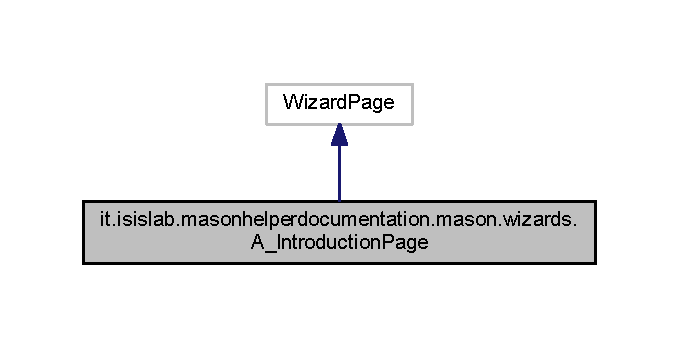
\includegraphics[width=326pt]{classit_1_1isislab_1_1masonhelperdocumentation_1_1mason_1_1wizards_1_1_a___introduction_page__inherit__graph}
\end{center}
\end{figure}


Collaboration diagram for it.\-isislab.\-masonhelperdocumentation.\-mason.\-wizards.\-A\-\_\-\-Introduction\-Page\-:\nopagebreak
\begin{figure}[H]
\begin{center}
\leavevmode
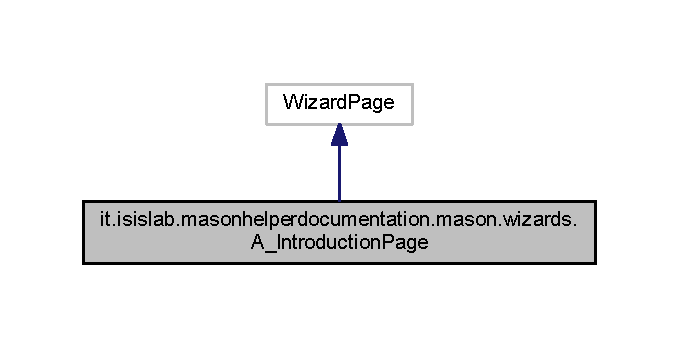
\includegraphics[width=326pt]{classit_1_1isislab_1_1masonhelperdocumentation_1_1mason_1_1wizards_1_1_a___introduction_page__coll__graph}
\end{center}
\end{figure}
\subsection*{Public Member Functions}
\begin{DoxyCompactItemize}
\item 
\hyperlink{classit_1_1isislab_1_1masonhelperdocumentation_1_1mason_1_1wizards_1_1_a___introduction_page_a0ad4b7c0d0d63d7408d41ae0ea64cc74}{A\-\_\-\-Introduction\-Page} ()
\item 
void \hyperlink{classit_1_1isislab_1_1masonhelperdocumentation_1_1mason_1_1wizards_1_1_a___introduction_page_ab2150ace9b2c3717fafb9880f1078e17}{create\-Control} (Composite parent)
\item 
I\-Wizard\-Page \hyperlink{classit_1_1isislab_1_1masonhelperdocumentation_1_1mason_1_1wizards_1_1_a___introduction_page_a2cf283c12319487dc35d2bb428327133}{get\-Next\-Page} ()
\end{DoxyCompactItemize}
\subsection*{Static Private Attributes}
\begin{DoxyCompactItemize}
\item 
static String \hyperlink{classit_1_1isislab_1_1masonhelperdocumentation_1_1mason_1_1wizards_1_1_a___introduction_page_a48f9e6bddf3bb2d7ba3995b09dd4da0b}{introduction}
\end{DoxyCompactItemize}


\subsection{Constructor \& Destructor Documentation}
\hypertarget{classit_1_1isislab_1_1masonhelperdocumentation_1_1mason_1_1wizards_1_1_a___introduction_page_a0ad4b7c0d0d63d7408d41ae0ea64cc74}{\index{it\-::isislab\-::masonhelperdocumentation\-::mason\-::wizards\-::\-A\-\_\-\-Introduction\-Page@{it\-::isislab\-::masonhelperdocumentation\-::mason\-::wizards\-::\-A\-\_\-\-Introduction\-Page}!A\-\_\-\-Introduction\-Page@{A\-\_\-\-Introduction\-Page}}
\index{A\-\_\-\-Introduction\-Page@{A\-\_\-\-Introduction\-Page}!it::isislab::masonhelperdocumentation::mason::wizards::A_IntroductionPage@{it\-::isislab\-::masonhelperdocumentation\-::mason\-::wizards\-::\-A\-\_\-\-Introduction\-Page}}
\subsubsection[{A\-\_\-\-Introduction\-Page}]{\setlength{\rightskip}{0pt plus 5cm}it.\-isislab.\-masonhelperdocumentation.\-mason.\-wizards.\-A\-\_\-\-Introduction\-Page.\-A\-\_\-\-Introduction\-Page (
\begin{DoxyParamCaption}
{}
\end{DoxyParamCaption}
)}}\label{classit_1_1isislab_1_1masonhelperdocumentation_1_1mason_1_1wizards_1_1_a___introduction_page_a0ad4b7c0d0d63d7408d41ae0ea64cc74}
Create the wizard. 
\begin{DoxyCode}
29                                 \{
30         super(\textcolor{stringliteral}{"wizardPage"});
31         setTitle(\textcolor{stringliteral}{"ABMs ODD documentation"});
32         setDescription(\textcolor{stringliteral}{"Welcome to ABMs ODD wizard"});
33     \}
\end{DoxyCode}


\subsection{Member Function Documentation}
\hypertarget{classit_1_1isislab_1_1masonhelperdocumentation_1_1mason_1_1wizards_1_1_a___introduction_page_ab2150ace9b2c3717fafb9880f1078e17}{\index{it\-::isislab\-::masonhelperdocumentation\-::mason\-::wizards\-::\-A\-\_\-\-Introduction\-Page@{it\-::isislab\-::masonhelperdocumentation\-::mason\-::wizards\-::\-A\-\_\-\-Introduction\-Page}!create\-Control@{create\-Control}}
\index{create\-Control@{create\-Control}!it::isislab::masonhelperdocumentation::mason::wizards::A_IntroductionPage@{it\-::isislab\-::masonhelperdocumentation\-::mason\-::wizards\-::\-A\-\_\-\-Introduction\-Page}}
\subsubsection[{create\-Control}]{\setlength{\rightskip}{0pt plus 5cm}void it.\-isislab.\-masonhelperdocumentation.\-mason.\-wizards.\-A\-\_\-\-Introduction\-Page.\-create\-Control (
\begin{DoxyParamCaption}
\item[{Composite}]{parent}
\end{DoxyParamCaption}
)}}\label{classit_1_1isislab_1_1masonhelperdocumentation_1_1mason_1_1wizards_1_1_a___introduction_page_ab2150ace9b2c3717fafb9880f1078e17}
Create contents of the wizard. 
\begin{DoxyParams}{Parameters}
{\em parent} & \\
\hline
\end{DoxyParams}

\begin{DoxyCode}
39                                                 \{
40         Composite container = \textcolor{keyword}{new} Composite(parent, SWT.NONE);
41 
42         setControl(container);
43         
44         Label lblIntroduction = \textcolor{keyword}{new} Label(container, SWT.NONE);
45         lblIntroduction.setBounds(10, 10, 554, 189);
46         lblIntroduction.setText(\hyperlink{classit_1_1isislab_1_1masonhelperdocumentation_1_1mason_1_1wizards_1_1_a___introduction_page_a48f9e6bddf3bb2d7ba3995b09dd4da0b}{introduction});
47     \}
\end{DoxyCode}
\hypertarget{classit_1_1isislab_1_1masonhelperdocumentation_1_1mason_1_1wizards_1_1_a___introduction_page_a2cf283c12319487dc35d2bb428327133}{\index{it\-::isislab\-::masonhelperdocumentation\-::mason\-::wizards\-::\-A\-\_\-\-Introduction\-Page@{it\-::isislab\-::masonhelperdocumentation\-::mason\-::wizards\-::\-A\-\_\-\-Introduction\-Page}!get\-Next\-Page@{get\-Next\-Page}}
\index{get\-Next\-Page@{get\-Next\-Page}!it::isislab::masonhelperdocumentation::mason::wizards::A_IntroductionPage@{it\-::isislab\-::masonhelperdocumentation\-::mason\-::wizards\-::\-A\-\_\-\-Introduction\-Page}}
\subsubsection[{get\-Next\-Page}]{\setlength{\rightskip}{0pt plus 5cm}I\-Wizard\-Page it.\-isislab.\-masonhelperdocumentation.\-mason.\-wizards.\-A\-\_\-\-Introduction\-Page.\-get\-Next\-Page (
\begin{DoxyParamCaption}
{}
\end{DoxyParamCaption}
)}}\label{classit_1_1isislab_1_1masonhelperdocumentation_1_1mason_1_1wizards_1_1_a___introduction_page_a2cf283c12319487dc35d2bb428327133}

\begin{DoxyCode}
49                                     \{ 
50         A1\_ChooseOutput nextPage = \textcolor{keyword}{new} A1\_ChooseOutput();
51         ((MASONDocumentationWizard) super.getWizard()).addPage(nextPage);
52         \textcolor{keywordflow}{return} nextPage;
53     \}
\end{DoxyCode}


\subsection{Member Data Documentation}
\hypertarget{classit_1_1isislab_1_1masonhelperdocumentation_1_1mason_1_1wizards_1_1_a___introduction_page_a48f9e6bddf3bb2d7ba3995b09dd4da0b}{\index{it\-::isislab\-::masonhelperdocumentation\-::mason\-::wizards\-::\-A\-\_\-\-Introduction\-Page@{it\-::isislab\-::masonhelperdocumentation\-::mason\-::wizards\-::\-A\-\_\-\-Introduction\-Page}!introduction@{introduction}}
\index{introduction@{introduction}!it::isislab::masonhelperdocumentation::mason::wizards::A_IntroductionPage@{it\-::isislab\-::masonhelperdocumentation\-::mason\-::wizards\-::\-A\-\_\-\-Introduction\-Page}}
\subsubsection[{introduction}]{\setlength{\rightskip}{0pt plus 5cm}String it.\-isislab.\-masonhelperdocumentation.\-mason.\-wizards.\-A\-\_\-\-Introduction\-Page.\-introduction\hspace{0.3cm}{\ttfamily [static]}, {\ttfamily [private]}}}\label{classit_1_1isislab_1_1masonhelperdocumentation_1_1mason_1_1wizards_1_1_a___introduction_page_a48f9e6bddf3bb2d7ba3995b09dd4da0b}
{\bfseries Initial value\-:}
\begin{DoxyCode}
= \textcolor{stringliteral}{"This wizard will auto-generate ABMs "}
                            + \textcolor{stringliteral}{"documentation with the standard ODD format. The objectives of \(\backslash\)n"}
                            + \textcolor{stringliteral}{"ODD are to make model descriptions more understandable and "}
                            + \textcolor{stringliteral}{"complete, thereby making ABMs less \(\backslash\)nsubject to criticism for "}
                            + \textcolor{stringliteral}{"being irreproducible.\(\backslash\)n\(\backslash\)n"}
                            + \textcolor{stringliteral}{"Elements of ODD:\(\backslash\)n"}
                            + \textcolor{stringliteral}{"   1. Purpose\(\backslash\)n"}
                            + \textcolor{stringliteral}{"   2. Entities, state variables, and scales\(\backslash\)n"}
                            + \textcolor{stringliteral}{"   3. Process overview and scheduling\(\backslash\)n"}
                            + \textcolor{stringliteral}{"   4. Design concepts\(\backslash\)n"}
                            + \textcolor{stringliteral}{"   5. Initialization\(\backslash\)n"}  
                            + \textcolor{stringliteral}{"   6. Input data\(\backslash\)n"}
                            + \textcolor{stringliteral}{"   7. Submodels"}
\end{DoxyCode}


The documentation for this class was generated from the following file\-:\begin{DoxyCompactItemize}
\item 
src/it/isislab/masonhelperdocumentation/mason/wizards/\hyperlink{_a___introduction_page_8java}{A\-\_\-\-Introduction\-Page.\-java}\end{DoxyCompactItemize}

\hypertarget{classit_1_1isislab_1_1masonhelperdocumentation_1_1analizer_1_1_agent_analizer}{\section{it.\-isislab.\-masonhelperdocumentation.\-analizer.\-Agent\-Analizer Class Reference}
\label{classit_1_1isislab_1_1masonhelperdocumentation_1_1analizer_1_1_agent_analizer}\index{it.\-isislab.\-masonhelperdocumentation.\-analizer.\-Agent\-Analizer@{it.\-isislab.\-masonhelperdocumentation.\-analizer.\-Agent\-Analizer}}
}


Inheritance diagram for it.\-isislab.\-masonhelperdocumentation.\-analizer.\-Agent\-Analizer\-:
\nopagebreak
\begin{figure}[H]
\begin{center}
\leavevmode
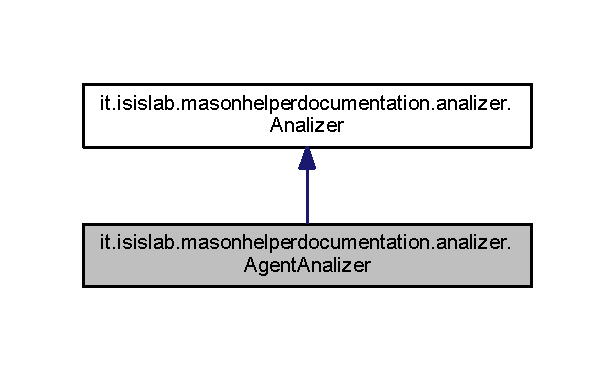
\includegraphics[width=295pt]{classit_1_1isislab_1_1masonhelperdocumentation_1_1analizer_1_1_agent_analizer__inherit__graph}
\end{center}
\end{figure}


Collaboration diagram for it.\-isislab.\-masonhelperdocumentation.\-analizer.\-Agent\-Analizer\-:
\nopagebreak
\begin{figure}[H]
\begin{center}
\leavevmode
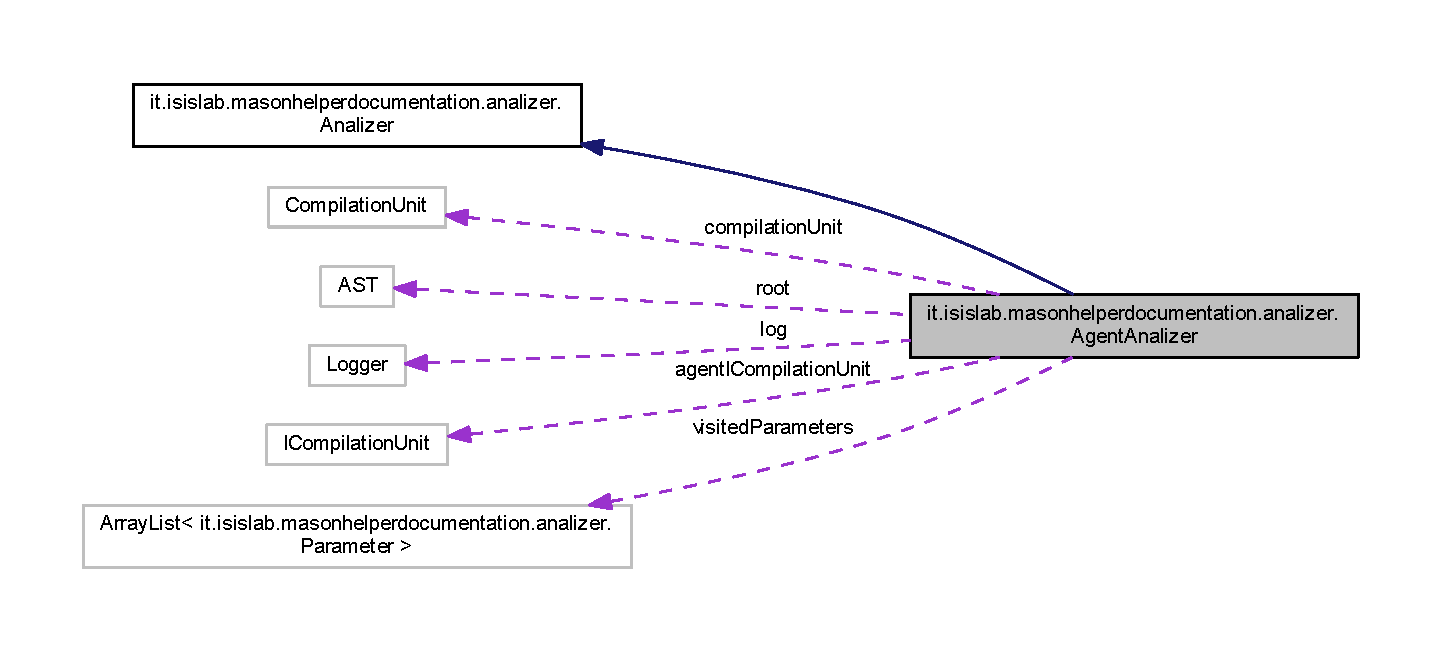
\includegraphics[width=350pt]{classit_1_1isislab_1_1masonhelperdocumentation_1_1analizer_1_1_agent_analizer__coll__graph}
\end{center}
\end{figure}
\subsection*{Public Member Functions}
\begin{DoxyCompactItemize}
\item 
\hyperlink{classit_1_1isislab_1_1masonhelperdocumentation_1_1analizer_1_1_agent_analizer_adc8b62d98bb421e6baa3373f3694fee8}{Agent\-Analizer} (I\-Compilation\-Unit agent\-C\-U)
\item 
void \hyperlink{classit_1_1isislab_1_1masonhelperdocumentation_1_1analizer_1_1_agent_analizer_aa330ee12112641e1ba3d9acedb9401b9}{rewrite} ()
\item 
Javadoc \hyperlink{classit_1_1isislab_1_1masonhelperdocumentation_1_1analizer_1_1_agent_analizer_a4a819d1324aa806e8bc729bb5d6ce398}{get\-Model\-Description} ()
\item 
void \hyperlink{classit_1_1isislab_1_1masonhelperdocumentation_1_1analizer_1_1_agent_analizer_a1dcc3313d7fe6fa67fd3c27433b78763}{set\-Class\-Description} (String model\-Description)
\item 
Array\-List$<$ \hyperlink{classit_1_1isislab_1_1masonhelperdocumentation_1_1analizer_1_1_parameter}{Parameter} $>$ \hyperlink{classit_1_1isislab_1_1masonhelperdocumentation_1_1analizer_1_1_agent_analizer_aed0a62fd5108f41992ade938d6bcd9cc}{get\-Visited\-Parameters} ()
\item 
Array\-List$<$ \hyperlink{classit_1_1isislab_1_1masonhelperdocumentation_1_1analizer_1_1_parameter}{Parameter} $>$ \hyperlink{classit_1_1isislab_1_1masonhelperdocumentation_1_1analizer_1_1_agent_analizer_aa2e85956f4a23176c398294cf02d859d}{get\-Positions\-Parameter} ()
\item 
Compilation\-Unit \hyperlink{classit_1_1isislab_1_1masonhelperdocumentation_1_1analizer_1_1_agent_analizer_af956b9fdd9d6b6b97d4982cba816d441}{get\-Compilation\-Unit} ()
\item 
A\-S\-T \hyperlink{classit_1_1isislab_1_1masonhelperdocumentation_1_1analizer_1_1_agent_analizer_a32883fb3c910d96ba584549d27856ce1}{get\-Root} ()
\item 
String \hyperlink{classit_1_1isislab_1_1masonhelperdocumentation_1_1analizer_1_1_agent_analizer_a5f65d6f8f8c1a00b0b66fb3dd0ab37cb}{get\-Position\-Class} ()
\item 
boolean \hyperlink{classit_1_1isislab_1_1masonhelperdocumentation_1_1analizer_1_1_agent_analizer_a6be22d4f751e44b18796b10767b581d5}{already\-Visited} (\hyperlink{classit_1_1isislab_1_1masonhelperdocumentation_1_1analizer_1_1_parameter}{Parameter} p)
\item 
String \hyperlink{classit_1_1isislab_1_1masonhelperdocumentation_1_1analizer_1_1_agent_analizer_ace466e16439878a851eb63d5a11ddf43}{get\-Class\-Name} ()
\item 
String \hyperlink{classit_1_1isislab_1_1masonhelperdocumentation_1_1analizer_1_1_agent_analizer_aea58a6f4ec614b3778588784cb250dcb}{to\-String} ()
\end{DoxyCompactItemize}
\subsection*{Static Public Attributes}
\begin{DoxyCompactItemize}
\item 
static String\mbox{[}$\,$\mbox{]} \hyperlink{classit_1_1isislab_1_1masonhelperdocumentation_1_1analizer_1_1_agent_analizer_a9d8e56c5d7ee2102e06e509b301205bb}{position\-Class} = \{\char`\"{}Int2\-D\char`\"{}, \char`\"{}Double2\-D\char`\"{}, \char`\"{}Int3\-D\char`\"{}, \char`\"{}Double3\-D\char`\"{},\}
\item 
static String \hyperlink{classit_1_1isislab_1_1masonhelperdocumentation_1_1analizer_1_1_agent_analizer_ada4b9766b061207045f6b7110e7e8ed6}{steppable\-Description}
\end{DoxyCompactItemize}
\subsection*{Private Attributes}
\begin{DoxyCompactItemize}
\item 
I\-Compilation\-Unit \hyperlink{classit_1_1isislab_1_1masonhelperdocumentation_1_1analizer_1_1_agent_analizer_a5982c48c7c223886875d55c4b2383140}{agent\-I\-Compilation\-Unit}
\item 
Compilation\-Unit \hyperlink{classit_1_1isislab_1_1masonhelperdocumentation_1_1analizer_1_1_agent_analizer_a1fdd2196fdd7b7907ab94da91b8306f4}{compilation\-Unit}
\item 
A\-S\-T \hyperlink{classit_1_1isislab_1_1masonhelperdocumentation_1_1analizer_1_1_agent_analizer_a43035809f1965186296ce39327323a14}{root}
\item 
Array\-List$<$ \hyperlink{classit_1_1isislab_1_1masonhelperdocumentation_1_1analizer_1_1_parameter}{Parameter} $>$ \hyperlink{classit_1_1isislab_1_1masonhelperdocumentation_1_1analizer_1_1_agent_analizer_a631132645fb74a4498f033579556efa9}{visited\-Parameters}
\end{DoxyCompactItemize}
\subsection*{Static Private Attributes}
\begin{DoxyCompactItemize}
\item 
static Logger \hyperlink{classit_1_1isislab_1_1masonhelperdocumentation_1_1analizer_1_1_agent_analizer_a17da3ff078911c8a90212bab3681f31e}{log} = Logger.\-get\-Logger(\char`\"{}global\char`\"{})
\end{DoxyCompactItemize}


\subsection{Constructor \& Destructor Documentation}
\hypertarget{classit_1_1isislab_1_1masonhelperdocumentation_1_1analizer_1_1_agent_analizer_adc8b62d98bb421e6baa3373f3694fee8}{\index{it\-::isislab\-::masonhelperdocumentation\-::analizer\-::\-Agent\-Analizer@{it\-::isislab\-::masonhelperdocumentation\-::analizer\-::\-Agent\-Analizer}!Agent\-Analizer@{Agent\-Analizer}}
\index{Agent\-Analizer@{Agent\-Analizer}!it::isislab::masonhelperdocumentation::analizer::AgentAnalizer@{it\-::isislab\-::masonhelperdocumentation\-::analizer\-::\-Agent\-Analizer}}
\subsubsection[{Agent\-Analizer}]{\setlength{\rightskip}{0pt plus 5cm}it.\-isislab.\-masonhelperdocumentation.\-analizer.\-Agent\-Analizer.\-Agent\-Analizer (
\begin{DoxyParamCaption}
\item[{I\-Compilation\-Unit}]{agent\-C\-U}
\end{DoxyParamCaption}
)}}\label{classit_1_1isislab_1_1masonhelperdocumentation_1_1analizer_1_1_agent_analizer_adc8b62d98bb421e6baa3373f3694fee8}

\begin{DoxyCode}
30                                                    \{
31         \hyperlink{classit_1_1isislab_1_1masonhelperdocumentation_1_1analizer_1_1_agent_analizer_a5982c48c7c223886875d55c4b2383140}{agentICompilationUnit} = agentCU;
32         \hyperlink{classit_1_1isislab_1_1masonhelperdocumentation_1_1analizer_1_1_agent_analizer_a1fdd2196fdd7b7907ab94da91b8306f4}{compilationUnit} = GlobalUtility.getCompilationUnit(agentCU); 
33         \hyperlink{classit_1_1isislab_1_1masonhelperdocumentation_1_1analizer_1_1_agent_analizer_a43035809f1965186296ce39327323a14}{root} = GlobalUtility.getAstFromCompilationUnit(\hyperlink{classit_1_1isislab_1_1masonhelperdocumentation_1_1analizer_1_1_agent_analizer_a1fdd2196fdd7b7907ab94da91b8306f4}{compilationUnit});
34         \hyperlink{classit_1_1isislab_1_1masonhelperdocumentation_1_1analizer_1_1_agent_analizer_a631132645fb74a4498f033579556efa9}{visitedParameters} = \textcolor{keyword}{new} ArrayList<Parameter>();
35         log.info(\textcolor{stringliteral}{"AgentAnalizer created"});
36     \}
\end{DoxyCode}


\subsection{Member Function Documentation}
\hypertarget{classit_1_1isislab_1_1masonhelperdocumentation_1_1analizer_1_1_agent_analizer_a6be22d4f751e44b18796b10767b581d5}{\index{it\-::isislab\-::masonhelperdocumentation\-::analizer\-::\-Agent\-Analizer@{it\-::isislab\-::masonhelperdocumentation\-::analizer\-::\-Agent\-Analizer}!already\-Visited@{already\-Visited}}
\index{already\-Visited@{already\-Visited}!it::isislab::masonhelperdocumentation::analizer::AgentAnalizer@{it\-::isislab\-::masonhelperdocumentation\-::analizer\-::\-Agent\-Analizer}}
\subsubsection[{already\-Visited}]{\setlength{\rightskip}{0pt plus 5cm}boolean it.\-isislab.\-masonhelperdocumentation.\-analizer.\-Agent\-Analizer.\-already\-Visited (
\begin{DoxyParamCaption}
\item[{{\bf Parameter}}]{p}
\end{DoxyParamCaption}
)}}\label{classit_1_1isislab_1_1masonhelperdocumentation_1_1analizer_1_1_agent_analizer_a6be22d4f751e44b18796b10767b581d5}
Return true if parameter p has been already visited. For 'visited' I mean that I already added this parameters to Simulation\-Group in some part of wizard 
\begin{DoxyParams}{Parameters}
{\em p} & \\
\hline
\end{DoxyParams}
\begin{DoxyReturn}{Returns}

\end{DoxyReturn}

\begin{DoxyCode}
135                                               \{
136         \textcolor{keywordflow}{for} (Parameter par : \hyperlink{classit_1_1isislab_1_1masonhelperdocumentation_1_1analizer_1_1_agent_analizer_a631132645fb74a4498f033579556efa9}{visitedParameters})\{
137             \textcolor{keywordflow}{if} (par.equals(p))  \textcolor{keywordflow}{return} \textcolor{keyword}{true};
138         \}
139         \textcolor{keywordflow}{return} \textcolor{keyword}{false};
140     \}
\end{DoxyCode}


Here is the caller graph for this function\-:
\nopagebreak
\begin{figure}[H]
\begin{center}
\leavevmode
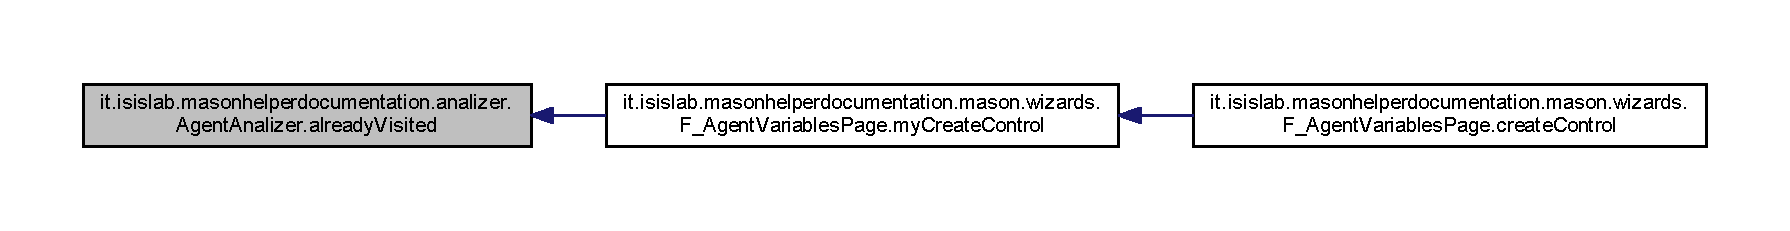
\includegraphics[width=350pt]{classit_1_1isislab_1_1masonhelperdocumentation_1_1analizer_1_1_agent_analizer_a6be22d4f751e44b18796b10767b581d5_icgraph}
\end{center}
\end{figure}


\hypertarget{classit_1_1isislab_1_1masonhelperdocumentation_1_1analizer_1_1_agent_analizer_ace466e16439878a851eb63d5a11ddf43}{\index{it\-::isislab\-::masonhelperdocumentation\-::analizer\-::\-Agent\-Analizer@{it\-::isislab\-::masonhelperdocumentation\-::analizer\-::\-Agent\-Analizer}!get\-Class\-Name@{get\-Class\-Name}}
\index{get\-Class\-Name@{get\-Class\-Name}!it::isislab::masonhelperdocumentation::analizer::AgentAnalizer@{it\-::isislab\-::masonhelperdocumentation\-::analizer\-::\-Agent\-Analizer}}
\subsubsection[{get\-Class\-Name}]{\setlength{\rightskip}{0pt plus 5cm}String it.\-isislab.\-masonhelperdocumentation.\-analizer.\-Agent\-Analizer.\-get\-Class\-Name (
\begin{DoxyParamCaption}
{}
\end{DoxyParamCaption}
)}}\label{classit_1_1isislab_1_1masonhelperdocumentation_1_1analizer_1_1_agent_analizer_ace466e16439878a851eb63d5a11ddf43}
Return class name of this agent. \begin{DoxyReturn}{Returns}

\end{DoxyReturn}

\begin{DoxyCode}
146                                 \{
147         \textcolor{keywordflow}{return} agentICompilationUnit.getElementName();
148     \}
\end{DoxyCode}


Here is the caller graph for this function\-:
\nopagebreak
\begin{figure}[H]
\begin{center}
\leavevmode
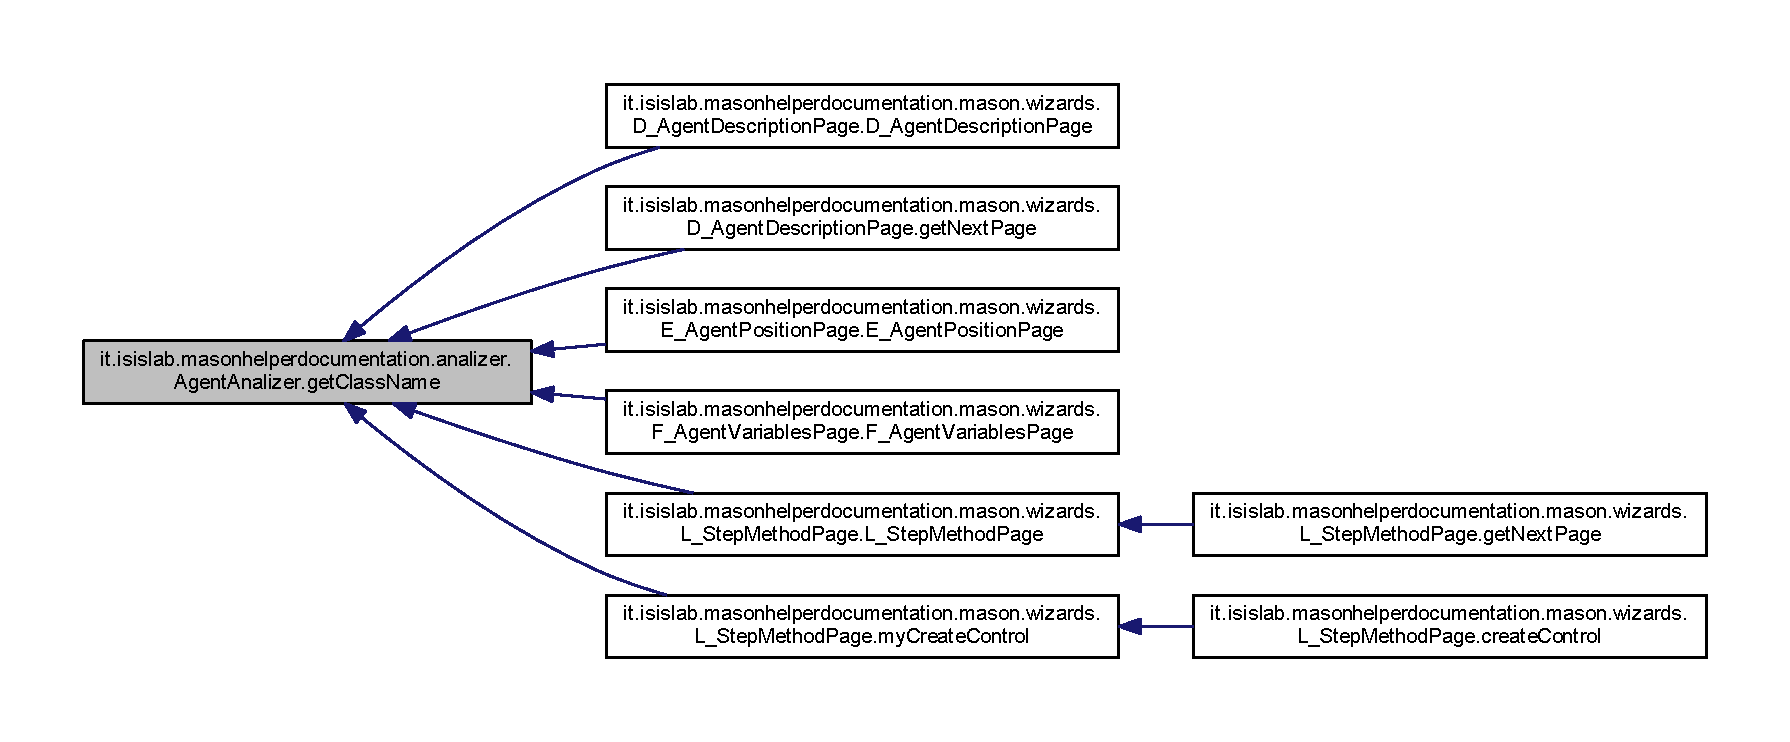
\includegraphics[width=350pt]{classit_1_1isislab_1_1masonhelperdocumentation_1_1analizer_1_1_agent_analizer_ace466e16439878a851eb63d5a11ddf43_icgraph}
\end{center}
\end{figure}


\hypertarget{classit_1_1isislab_1_1masonhelperdocumentation_1_1analizer_1_1_agent_analizer_af956b9fdd9d6b6b97d4982cba816d441}{\index{it\-::isislab\-::masonhelperdocumentation\-::analizer\-::\-Agent\-Analizer@{it\-::isislab\-::masonhelperdocumentation\-::analizer\-::\-Agent\-Analizer}!get\-Compilation\-Unit@{get\-Compilation\-Unit}}
\index{get\-Compilation\-Unit@{get\-Compilation\-Unit}!it::isislab::masonhelperdocumentation::analizer::AgentAnalizer@{it\-::isislab\-::masonhelperdocumentation\-::analizer\-::\-Agent\-Analizer}}
\subsubsection[{get\-Compilation\-Unit}]{\setlength{\rightskip}{0pt plus 5cm}Compilation\-Unit it.\-isislab.\-masonhelperdocumentation.\-analizer.\-Agent\-Analizer.\-get\-Compilation\-Unit (
\begin{DoxyParamCaption}
{}
\end{DoxyParamCaption}
)}}\label{classit_1_1isislab_1_1masonhelperdocumentation_1_1analizer_1_1_agent_analizer_af956b9fdd9d6b6b97d4982cba816d441}
Retirn Compilation\-Unit. \begin{DoxyReturn}{Returns}

\end{DoxyReturn}

\begin{DoxyCode}
108                                                \{
109         \textcolor{keywordflow}{return} \hyperlink{classit_1_1isislab_1_1masonhelperdocumentation_1_1analizer_1_1_agent_analizer_a1fdd2196fdd7b7907ab94da91b8306f4}{compilationUnit};
110     \}
\end{DoxyCode}
\hypertarget{classit_1_1isislab_1_1masonhelperdocumentation_1_1analizer_1_1_agent_analizer_a4a819d1324aa806e8bc729bb5d6ce398}{\index{it\-::isislab\-::masonhelperdocumentation\-::analizer\-::\-Agent\-Analizer@{it\-::isislab\-::masonhelperdocumentation\-::analizer\-::\-Agent\-Analizer}!get\-Model\-Description@{get\-Model\-Description}}
\index{get\-Model\-Description@{get\-Model\-Description}!it::isislab::masonhelperdocumentation::analizer::AgentAnalizer@{it\-::isislab\-::masonhelperdocumentation\-::analizer\-::\-Agent\-Analizer}}
\subsubsection[{get\-Model\-Description}]{\setlength{\rightskip}{0pt plus 5cm}Javadoc it.\-isislab.\-masonhelperdocumentation.\-analizer.\-Agent\-Analizer.\-get\-Model\-Description (
\begin{DoxyParamCaption}
{}
\end{DoxyParamCaption}
)}}\label{classit_1_1isislab_1_1masonhelperdocumentation_1_1analizer_1_1_agent_analizer_a4a819d1324aa806e8bc729bb5d6ce398}
This method return the descriprion of this Agent. \begin{DoxyReturn}{Returns}
Javadoc\-Comment if there is a description; else null. 
\end{DoxyReturn}

\begin{DoxyCode}
61                                         \{
62         List<TypeDeclaration> types = compilationUnit.types();
63         TypeDeclaration agent = types.get(0);
64         \textcolor{keywordflow}{return} agent.getJavadoc();
65     \}
\end{DoxyCode}
\hypertarget{classit_1_1isislab_1_1masonhelperdocumentation_1_1analizer_1_1_agent_analizer_a5f65d6f8f8c1a00b0b66fb3dd0ab37cb}{\index{it\-::isislab\-::masonhelperdocumentation\-::analizer\-::\-Agent\-Analizer@{it\-::isislab\-::masonhelperdocumentation\-::analizer\-::\-Agent\-Analizer}!get\-Position\-Class@{get\-Position\-Class}}
\index{get\-Position\-Class@{get\-Position\-Class}!it::isislab::masonhelperdocumentation::analizer::AgentAnalizer@{it\-::isislab\-::masonhelperdocumentation\-::analizer\-::\-Agent\-Analizer}}
\subsubsection[{get\-Position\-Class}]{\setlength{\rightskip}{0pt plus 5cm}String it.\-isislab.\-masonhelperdocumentation.\-analizer.\-Agent\-Analizer.\-get\-Position\-Class (
\begin{DoxyParamCaption}
{}
\end{DoxyParamCaption}
)}}\label{classit_1_1isislab_1_1masonhelperdocumentation_1_1analizer_1_1_agent_analizer_a5f65d6f8f8c1a00b0b66fb3dd0ab37cb}
Return a string representation of position\-Class array. \begin{DoxyReturn}{Returns}

\end{DoxyReturn}

\begin{DoxyCode}
120                                     \{
121         String toReturn = \textcolor{stringliteral}{""};
122         \textcolor{keywordflow}{for} (\textcolor{keywordtype}{int} i=0; i<positionClass.length; i++)\{
123             toReturn = toReturn + \hyperlink{classit_1_1isislab_1_1masonhelperdocumentation_1_1analizer_1_1_agent_analizer_a9d8e56c5d7ee2102e06e509b301205bb}{positionClass}[i] + \textcolor{stringliteral}{" - "};
124         \}
125         \textcolor{keywordflow}{return} toReturn.substring(0, toReturn.length()-3);
126     \}
\end{DoxyCode}
\hypertarget{classit_1_1isislab_1_1masonhelperdocumentation_1_1analizer_1_1_agent_analizer_aa2e85956f4a23176c398294cf02d859d}{\index{it\-::isislab\-::masonhelperdocumentation\-::analizer\-::\-Agent\-Analizer@{it\-::isislab\-::masonhelperdocumentation\-::analizer\-::\-Agent\-Analizer}!get\-Positions\-Parameter@{get\-Positions\-Parameter}}
\index{get\-Positions\-Parameter@{get\-Positions\-Parameter}!it::isislab::masonhelperdocumentation::analizer::AgentAnalizer@{it\-::isislab\-::masonhelperdocumentation\-::analizer\-::\-Agent\-Analizer}}
\subsubsection[{get\-Positions\-Parameter}]{\setlength{\rightskip}{0pt plus 5cm}Array\-List$<${\bf Parameter}$>$ it.\-isislab.\-masonhelperdocumentation.\-analizer.\-Agent\-Analizer.\-get\-Positions\-Parameter (
\begin{DoxyParamCaption}
{}
\end{DoxyParamCaption}
)}}\label{classit_1_1isislab_1_1masonhelperdocumentation_1_1analizer_1_1_agent_analizer_aa2e85956f4a23176c398294cf02d859d}
This method extract a list of Variable\-Declaration\-Fragment for positions variables. \begin{DoxyReturn}{Returns}
Array\-List of positions as Variable\-Declaration\-Fragment 
\end{DoxyReturn}

\begin{DoxyCode}
93                                                        \{
94         \textcolor{keywordflow}{if} (GlobalUtility.getAllParameters(\hyperlink{classit_1_1isislab_1_1masonhelperdocumentation_1_1analizer_1_1_agent_analizer_a1fdd2196fdd7b7907ab94da91b8306f4}{compilationUnit}) == null) \textcolor{keywordflow}{return} null;
95         ArrayList<Parameter> toReturn = \textcolor{keyword}{new} ArrayList<Parameter>();
96         \textcolor{keywordflow}{for} (Parameter p : GlobalUtility.getAllParameters(\hyperlink{classit_1_1isislab_1_1masonhelperdocumentation_1_1analizer_1_1_agent_analizer_a1fdd2196fdd7b7907ab94da91b8306f4}{compilationUnit}))\{
97                 \textcolor{keywordflow}{for} (\textcolor{keywordtype}{int} i=0; i<positionClass.length; i++)\{
98                     \textcolor{keywordflow}{if} (p.getVariableType().equalsIgnoreCase(\hyperlink{classit_1_1isislab_1_1masonhelperdocumentation_1_1analizer_1_1_agent_analizer_a9d8e56c5d7ee2102e06e509b301205bb}{positionClass}[i]))    
      toReturn.add(p);
99                 \}               
100         \}
101         \textcolor{keywordflow}{return} toReturn;
102     \}   
\end{DoxyCode}


Here is the call graph for this function\-:
\nopagebreak
\begin{figure}[H]
\begin{center}
\leavevmode
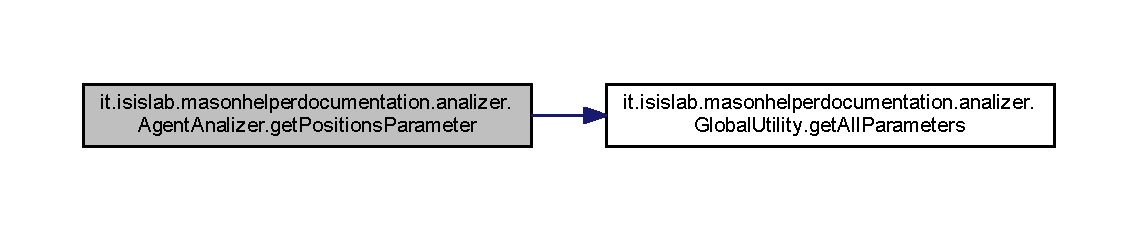
\includegraphics[width=350pt]{classit_1_1isislab_1_1masonhelperdocumentation_1_1analizer_1_1_agent_analizer_aa2e85956f4a23176c398294cf02d859d_cgraph}
\end{center}
\end{figure}




Here is the caller graph for this function\-:
\nopagebreak
\begin{figure}[H]
\begin{center}
\leavevmode
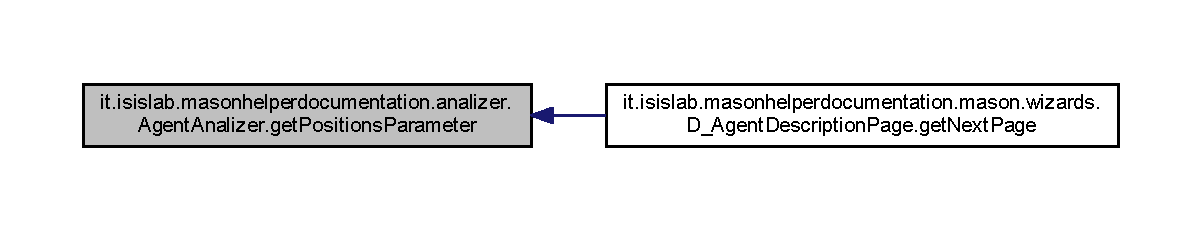
\includegraphics[width=350pt]{classit_1_1isislab_1_1masonhelperdocumentation_1_1analizer_1_1_agent_analizer_aa2e85956f4a23176c398294cf02d859d_icgraph}
\end{center}
\end{figure}


\hypertarget{classit_1_1isislab_1_1masonhelperdocumentation_1_1analizer_1_1_agent_analizer_a32883fb3c910d96ba584549d27856ce1}{\index{it\-::isislab\-::masonhelperdocumentation\-::analizer\-::\-Agent\-Analizer@{it\-::isislab\-::masonhelperdocumentation\-::analizer\-::\-Agent\-Analizer}!get\-Root@{get\-Root}}
\index{get\-Root@{get\-Root}!it::isislab::masonhelperdocumentation::analizer::AgentAnalizer@{it\-::isislab\-::masonhelperdocumentation\-::analizer\-::\-Agent\-Analizer}}
\subsubsection[{get\-Root}]{\setlength{\rightskip}{0pt plus 5cm}A\-S\-T it.\-isislab.\-masonhelperdocumentation.\-analizer.\-Agent\-Analizer.\-get\-Root (
\begin{DoxyParamCaption}
{}
\end{DoxyParamCaption}
)}}\label{classit_1_1isislab_1_1masonhelperdocumentation_1_1analizer_1_1_agent_analizer_a32883fb3c910d96ba584549d27856ce1}

\begin{DoxyCode}
112                         \{
113         \textcolor{keywordflow}{return} \hyperlink{classit_1_1isislab_1_1masonhelperdocumentation_1_1analizer_1_1_agent_analizer_a43035809f1965186296ce39327323a14}{root};
114     \}
\end{DoxyCode}
\hypertarget{classit_1_1isislab_1_1masonhelperdocumentation_1_1analizer_1_1_agent_analizer_aed0a62fd5108f41992ade938d6bcd9cc}{\index{it\-::isislab\-::masonhelperdocumentation\-::analizer\-::\-Agent\-Analizer@{it\-::isislab\-::masonhelperdocumentation\-::analizer\-::\-Agent\-Analizer}!get\-Visited\-Parameters@{get\-Visited\-Parameters}}
\index{get\-Visited\-Parameters@{get\-Visited\-Parameters}!it::isislab::masonhelperdocumentation::analizer::AgentAnalizer@{it\-::isislab\-::masonhelperdocumentation\-::analizer\-::\-Agent\-Analizer}}
\subsubsection[{get\-Visited\-Parameters}]{\setlength{\rightskip}{0pt plus 5cm}Array\-List$<${\bf Parameter}$>$ it.\-isislab.\-masonhelperdocumentation.\-analizer.\-Agent\-Analizer.\-get\-Visited\-Parameters (
\begin{DoxyParamCaption}
{}
\end{DoxyParamCaption}
)}}\label{classit_1_1isislab_1_1masonhelperdocumentation_1_1analizer_1_1_agent_analizer_aed0a62fd5108f41992ade938d6bcd9cc}
Return a list of visited parameter (visited means that parameters are already in Simulation\-Group). \begin{DoxyReturn}{Returns}

\end{DoxyReturn}

\begin{DoxyCode}
84                                                        \{
85         \textcolor{keywordflow}{return} \hyperlink{classit_1_1isislab_1_1masonhelperdocumentation_1_1analizer_1_1_agent_analizer_a631132645fb74a4498f033579556efa9}{visitedParameters};
86     \}
\end{DoxyCode}
\hypertarget{classit_1_1isislab_1_1masonhelperdocumentation_1_1analizer_1_1_agent_analizer_aa330ee12112641e1ba3d9acedb9401b9}{\index{it\-::isislab\-::masonhelperdocumentation\-::analizer\-::\-Agent\-Analizer@{it\-::isislab\-::masonhelperdocumentation\-::analizer\-::\-Agent\-Analizer}!rewrite@{rewrite}}
\index{rewrite@{rewrite}!it::isislab::masonhelperdocumentation::analizer::AgentAnalizer@{it\-::isislab\-::masonhelperdocumentation\-::analizer\-::\-Agent\-Analizer}}
\subsubsection[{rewrite}]{\setlength{\rightskip}{0pt plus 5cm}void it.\-isislab.\-masonhelperdocumentation.\-analizer.\-Agent\-Analizer.\-rewrite (
\begin{DoxyParamCaption}
{}
\end{DoxyParamCaption}
)}}\label{classit_1_1isislab_1_1masonhelperdocumentation_1_1analizer_1_1_agent_analizer_aa330ee12112641e1ba3d9acedb9401b9}


Implements \hyperlink{interfaceit_1_1isislab_1_1masonhelperdocumentation_1_1analizer_1_1_analizer_ac6b1ee8319b40e0fa6367392dc5de138}{it.\-isislab.\-masonhelperdocumentation.\-analizer.\-Analizer}.


\begin{DoxyCode}
39                           \{
40         File sourceFile = \textcolor{keyword}{new} File(\hyperlink{classit_1_1isislab_1_1masonhelperdocumentation_1_1analizer_1_1_agent_analizer_a5982c48c7c223886875d55c4b2383140}{agentICompilationUnit}.getResource().getRawLocation(
      ).toOSString());
41         FileOutputStream fooStream;
42         \textcolor{keywordflow}{try} \{
43             fooStream = \textcolor{keyword}{new} FileOutputStream(sourceFile, \textcolor{keyword}{false});
44             String code = compilationUnit.toString();
45             byte[] myBytes = code.getBytes();
46             fooStream.write(myBytes);
47             fooStream.close();
48         \} \textcolor{keywordflow}{catch} (FileNotFoundException e) \{
49             log.severe(\textcolor{stringliteral}{"Agent file not found to: "} + agentICompilationUnit.getResource().getRawLocation()
      .toOSString() + \textcolor{stringliteral}{"."});
50             e.printStackTrace();
51         \} \textcolor{keywordflow}{catch} (IOException e) \{
52             e.printStackTrace();
53         \}       
54     \}
\end{DoxyCode}
\hypertarget{classit_1_1isislab_1_1masonhelperdocumentation_1_1analizer_1_1_agent_analizer_a1dcc3313d7fe6fa67fd3c27433b78763}{\index{it\-::isislab\-::masonhelperdocumentation\-::analizer\-::\-Agent\-Analizer@{it\-::isislab\-::masonhelperdocumentation\-::analizer\-::\-Agent\-Analizer}!set\-Class\-Description@{set\-Class\-Description}}
\index{set\-Class\-Description@{set\-Class\-Description}!it::isislab::masonhelperdocumentation::analizer::AgentAnalizer@{it\-::isislab\-::masonhelperdocumentation\-::analizer\-::\-Agent\-Analizer}}
\subsubsection[{set\-Class\-Description}]{\setlength{\rightskip}{0pt plus 5cm}void it.\-isislab.\-masonhelperdocumentation.\-analizer.\-Agent\-Analizer.\-set\-Class\-Description (
\begin{DoxyParamCaption}
\item[{String}]{model\-Description}
\end{DoxyParamCaption}
)}}\label{classit_1_1isislab_1_1masonhelperdocumentation_1_1analizer_1_1_agent_analizer_a1dcc3313d7fe6fa67fd3c27433b78763}
This method set the description of model to model\-Description value. 
\begin{DoxyParams}{Parameters}
{\em model\-Description} & \\
\hline
\end{DoxyParams}

\begin{DoxyCode}
72                                                             \{
73         List<TypeDeclaration> types = compilationUnit.types();      
74         TypeDeclaration agent = types.get(0);   \textcolor{comment}{//get class definition (element in position 0)}
75         modelDescription = \textcolor{stringliteral}{"@ingroup entities\(\backslash\)n*\(\backslash\)n*"} + GlobalUtility.surroundWithSpan(
      \hyperlink{classit_1_1isislab_1_1masonhelperdocumentation_1_1analizer_1_1_global_utility_aec864cd710b27ece609c5a6093211ff4}{GlobalUtility.userOutputColor}, modelDescription);  
76         GlobalUtility.setJavadocToType(\hyperlink{classit_1_1isislab_1_1masonhelperdocumentation_1_1analizer_1_1_agent_analizer_a43035809f1965186296ce39327323a14}{root}, agent, modelDescription);
77     \}
\end{DoxyCode}
\hypertarget{classit_1_1isislab_1_1masonhelperdocumentation_1_1analizer_1_1_agent_analizer_aea58a6f4ec614b3778588784cb250dcb}{\index{it\-::isislab\-::masonhelperdocumentation\-::analizer\-::\-Agent\-Analizer@{it\-::isislab\-::masonhelperdocumentation\-::analizer\-::\-Agent\-Analizer}!to\-String@{to\-String}}
\index{to\-String@{to\-String}!it::isislab::masonhelperdocumentation::analizer::AgentAnalizer@{it\-::isislab\-::masonhelperdocumentation\-::analizer\-::\-Agent\-Analizer}}
\subsubsection[{to\-String}]{\setlength{\rightskip}{0pt plus 5cm}String it.\-isislab.\-masonhelperdocumentation.\-analizer.\-Agent\-Analizer.\-to\-String (
\begin{DoxyParamCaption}
{}
\end{DoxyParamCaption}
)}}\label{classit_1_1isislab_1_1masonhelperdocumentation_1_1analizer_1_1_agent_analizer_aea58a6f4ec614b3778588784cb250dcb}

\begin{DoxyCode}
150                             \{
151         \textcolor{keywordflow}{return} compilationUnit.toString();
152     \}
\end{DoxyCode}


\subsection{Member Data Documentation}
\hypertarget{classit_1_1isislab_1_1masonhelperdocumentation_1_1analizer_1_1_agent_analizer_a5982c48c7c223886875d55c4b2383140}{\index{it\-::isislab\-::masonhelperdocumentation\-::analizer\-::\-Agent\-Analizer@{it\-::isislab\-::masonhelperdocumentation\-::analizer\-::\-Agent\-Analizer}!agent\-I\-Compilation\-Unit@{agent\-I\-Compilation\-Unit}}
\index{agent\-I\-Compilation\-Unit@{agent\-I\-Compilation\-Unit}!it::isislab::masonhelperdocumentation::analizer::AgentAnalizer@{it\-::isislab\-::masonhelperdocumentation\-::analizer\-::\-Agent\-Analizer}}
\subsubsection[{agent\-I\-Compilation\-Unit}]{\setlength{\rightskip}{0pt plus 5cm}I\-Compilation\-Unit it.\-isislab.\-masonhelperdocumentation.\-analizer.\-Agent\-Analizer.\-agent\-I\-Compilation\-Unit\hspace{0.3cm}{\ttfamily [private]}}}\label{classit_1_1isislab_1_1masonhelperdocumentation_1_1analizer_1_1_agent_analizer_a5982c48c7c223886875d55c4b2383140}
\hypertarget{classit_1_1isislab_1_1masonhelperdocumentation_1_1analizer_1_1_agent_analizer_a1fdd2196fdd7b7907ab94da91b8306f4}{\index{it\-::isislab\-::masonhelperdocumentation\-::analizer\-::\-Agent\-Analizer@{it\-::isislab\-::masonhelperdocumentation\-::analizer\-::\-Agent\-Analizer}!compilation\-Unit@{compilation\-Unit}}
\index{compilation\-Unit@{compilation\-Unit}!it::isislab::masonhelperdocumentation::analizer::AgentAnalizer@{it\-::isislab\-::masonhelperdocumentation\-::analizer\-::\-Agent\-Analizer}}
\subsubsection[{compilation\-Unit}]{\setlength{\rightskip}{0pt plus 5cm}Compilation\-Unit it.\-isislab.\-masonhelperdocumentation.\-analizer.\-Agent\-Analizer.\-compilation\-Unit\hspace{0.3cm}{\ttfamily [private]}}}\label{classit_1_1isislab_1_1masonhelperdocumentation_1_1analizer_1_1_agent_analizer_a1fdd2196fdd7b7907ab94da91b8306f4}
\hypertarget{classit_1_1isislab_1_1masonhelperdocumentation_1_1analizer_1_1_agent_analizer_a17da3ff078911c8a90212bab3681f31e}{\index{it\-::isislab\-::masonhelperdocumentation\-::analizer\-::\-Agent\-Analizer@{it\-::isislab\-::masonhelperdocumentation\-::analizer\-::\-Agent\-Analizer}!log@{log}}
\index{log@{log}!it::isislab::masonhelperdocumentation::analizer::AgentAnalizer@{it\-::isislab\-::masonhelperdocumentation\-::analizer\-::\-Agent\-Analizer}}
\subsubsection[{log}]{\setlength{\rightskip}{0pt plus 5cm}Logger it.\-isislab.\-masonhelperdocumentation.\-analizer.\-Agent\-Analizer.\-log = Logger.\-get\-Logger(\char`\"{}global\char`\"{})\hspace{0.3cm}{\ttfamily [static]}, {\ttfamily [private]}}}\label{classit_1_1isislab_1_1masonhelperdocumentation_1_1analizer_1_1_agent_analizer_a17da3ff078911c8a90212bab3681f31e}
\hypertarget{classit_1_1isislab_1_1masonhelperdocumentation_1_1analizer_1_1_agent_analizer_a9d8e56c5d7ee2102e06e509b301205bb}{\index{it\-::isislab\-::masonhelperdocumentation\-::analizer\-::\-Agent\-Analizer@{it\-::isislab\-::masonhelperdocumentation\-::analizer\-::\-Agent\-Analizer}!position\-Class@{position\-Class}}
\index{position\-Class@{position\-Class}!it::isislab::masonhelperdocumentation::analizer::AgentAnalizer@{it\-::isislab\-::masonhelperdocumentation\-::analizer\-::\-Agent\-Analizer}}
\subsubsection[{position\-Class}]{\setlength{\rightskip}{0pt plus 5cm}String \mbox{[}$\,$\mbox{]} it.\-isislab.\-masonhelperdocumentation.\-analizer.\-Agent\-Analizer.\-position\-Class = \{\char`\"{}Int2\-D\char`\"{}, \char`\"{}Double2\-D\char`\"{}, \char`\"{}Int3\-D\char`\"{}, \char`\"{}Double3\-D\char`\"{},\}\hspace{0.3cm}{\ttfamily [static]}}}\label{classit_1_1isislab_1_1masonhelperdocumentation_1_1analizer_1_1_agent_analizer_a9d8e56c5d7ee2102e06e509b301205bb}
\hypertarget{classit_1_1isislab_1_1masonhelperdocumentation_1_1analizer_1_1_agent_analizer_a43035809f1965186296ce39327323a14}{\index{it\-::isislab\-::masonhelperdocumentation\-::analizer\-::\-Agent\-Analizer@{it\-::isislab\-::masonhelperdocumentation\-::analizer\-::\-Agent\-Analizer}!root@{root}}
\index{root@{root}!it::isislab::masonhelperdocumentation::analizer::AgentAnalizer@{it\-::isislab\-::masonhelperdocumentation\-::analizer\-::\-Agent\-Analizer}}
\subsubsection[{root}]{\setlength{\rightskip}{0pt plus 5cm}A\-S\-T it.\-isislab.\-masonhelperdocumentation.\-analizer.\-Agent\-Analizer.\-root\hspace{0.3cm}{\ttfamily [private]}}}\label{classit_1_1isislab_1_1masonhelperdocumentation_1_1analizer_1_1_agent_analizer_a43035809f1965186296ce39327323a14}
\hypertarget{classit_1_1isislab_1_1masonhelperdocumentation_1_1analizer_1_1_agent_analizer_ada4b9766b061207045f6b7110e7e8ed6}{\index{it\-::isislab\-::masonhelperdocumentation\-::analizer\-::\-Agent\-Analizer@{it\-::isislab\-::masonhelperdocumentation\-::analizer\-::\-Agent\-Analizer}!steppable\-Description@{steppable\-Description}}
\index{steppable\-Description@{steppable\-Description}!it::isislab::masonhelperdocumentation::analizer::AgentAnalizer@{it\-::isislab\-::masonhelperdocumentation\-::analizer\-::\-Agent\-Analizer}}
\subsubsection[{steppable\-Description}]{\setlength{\rightskip}{0pt plus 5cm}String it.\-isislab.\-masonhelperdocumentation.\-analizer.\-Agent\-Analizer.\-steppable\-Description\hspace{0.3cm}{\ttfamily [static]}}}\label{classit_1_1isislab_1_1masonhelperdocumentation_1_1analizer_1_1_agent_analizer_ada4b9766b061207045f6b7110e7e8ed6}
{\bfseries Initial value\-:}
\begin{DoxyCode}
= \textcolor{stringliteral}{"By being Steppable, this class represent an agent that can be\(\backslash\)n"}
            + \textcolor{stringliteral}{"on the Schedule to have its step method called at various times\(\backslash\)n"}
            + \textcolor{stringliteral}{"int the future. This graduates this agent from being a mere object\(\backslash\)n"}
            + \textcolor{stringliteral}{" in the simulation to being something potentially approximating a real agent.\(\backslash\)n"}
            + \textcolor{stringliteral}{"When this agent is stepped, it is passed the SimState.\(\backslash\)n"}
\end{DoxyCode}
\hypertarget{classit_1_1isislab_1_1masonhelperdocumentation_1_1analizer_1_1_agent_analizer_a631132645fb74a4498f033579556efa9}{\index{it\-::isislab\-::masonhelperdocumentation\-::analizer\-::\-Agent\-Analizer@{it\-::isislab\-::masonhelperdocumentation\-::analizer\-::\-Agent\-Analizer}!visited\-Parameters@{visited\-Parameters}}
\index{visited\-Parameters@{visited\-Parameters}!it::isislab::masonhelperdocumentation::analizer::AgentAnalizer@{it\-::isislab\-::masonhelperdocumentation\-::analizer\-::\-Agent\-Analizer}}
\subsubsection[{visited\-Parameters}]{\setlength{\rightskip}{0pt plus 5cm}Array\-List$<${\bf Parameter}$>$ it.\-isislab.\-masonhelperdocumentation.\-analizer.\-Agent\-Analizer.\-visited\-Parameters\hspace{0.3cm}{\ttfamily [private]}}}\label{classit_1_1isislab_1_1masonhelperdocumentation_1_1analizer_1_1_agent_analizer_a631132645fb74a4498f033579556efa9}


The documentation for this class was generated from the following file\-:\begin{DoxyCompactItemize}
\item 
src/it/isislab/masonhelperdocumentation/analizer/\hyperlink{_agent_analizer_8java}{Agent\-Analizer.\-java}\end{DoxyCompactItemize}

\hypertarget{interfaceit_1_1isislab_1_1masonhelperdocumentation_1_1analizer_1_1_analizer}{\section{it.\-isislab.\-masonhelperdocumentation.\-analizer.\-Analizer Interface Reference}
\label{interfaceit_1_1isislab_1_1masonhelperdocumentation_1_1analizer_1_1_analizer}\index{it.\-isislab.\-masonhelperdocumentation.\-analizer.\-Analizer@{it.\-isislab.\-masonhelperdocumentation.\-analizer.\-Analizer}}
}


Inheritance diagram for it.\-isislab.\-masonhelperdocumentation.\-analizer.\-Analizer\-:
\nopagebreak
\begin{figure}[H]
\begin{center}
\leavevmode
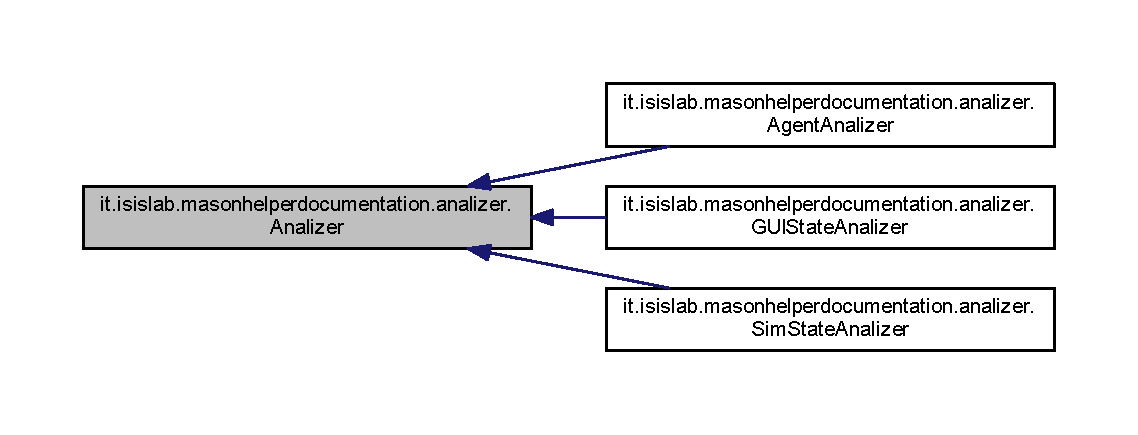
\includegraphics[width=350pt]{interfaceit_1_1isislab_1_1masonhelperdocumentation_1_1analizer_1_1_analizer__inherit__graph}
\end{center}
\end{figure}
\subsection*{Public Member Functions}
\begin{DoxyCompactItemize}
\item 
void \hyperlink{interfaceit_1_1isislab_1_1masonhelperdocumentation_1_1analizer_1_1_analizer_ac6b1ee8319b40e0fa6367392dc5de138}{rewrite} ()
\end{DoxyCompactItemize}


\subsection{Member Function Documentation}
\hypertarget{interfaceit_1_1isislab_1_1masonhelperdocumentation_1_1analizer_1_1_analizer_ac6b1ee8319b40e0fa6367392dc5de138}{\index{it\-::isislab\-::masonhelperdocumentation\-::analizer\-::\-Analizer@{it\-::isislab\-::masonhelperdocumentation\-::analizer\-::\-Analizer}!rewrite@{rewrite}}
\index{rewrite@{rewrite}!it::isislab::masonhelperdocumentation::analizer::Analizer@{it\-::isislab\-::masonhelperdocumentation\-::analizer\-::\-Analizer}}
\subsubsection[{rewrite}]{\setlength{\rightskip}{0pt plus 5cm}void it.\-isislab.\-masonhelperdocumentation.\-analizer.\-Analizer.\-rewrite (
\begin{DoxyParamCaption}
{}
\end{DoxyParamCaption}
)}}\label{interfaceit_1_1isislab_1_1masonhelperdocumentation_1_1analizer_1_1_analizer_ac6b1ee8319b40e0fa6367392dc5de138}


Implemented in \hyperlink{classit_1_1isislab_1_1masonhelperdocumentation_1_1analizer_1_1_sim_state_analizer_aa91938db714ec7b05134139ce741e61d}{it.\-isislab.\-masonhelperdocumentation.\-analizer.\-Sim\-State\-Analizer}, \hyperlink{classit_1_1isislab_1_1masonhelperdocumentation_1_1analizer_1_1_g_u_i_state_analizer_ade3afe629883da877a73f0a2527c4826}{it.\-isislab.\-masonhelperdocumentation.\-analizer.\-G\-U\-I\-State\-Analizer}, and \hyperlink{classit_1_1isislab_1_1masonhelperdocumentation_1_1analizer_1_1_agent_analizer_aa330ee12112641e1ba3d9acedb9401b9}{it.\-isislab.\-masonhelperdocumentation.\-analizer.\-Agent\-Analizer}.



The documentation for this interface was generated from the following file\-:\begin{DoxyCompactItemize}
\item 
git/masonhelperdocumentation/src/it/isislab/masonhelperdocumentation/analizer/\hyperlink{_analizer_8java}{Analizer.\-java}\end{DoxyCompactItemize}

\hypertarget{classit_1_1isislab_1_1masonhelperdocumentation_1_1mason_1_1wizards_1_1_b___project_information_page}{\section{it.\-isislab.\-masonhelperdocumentation.\-mason.\-wizards.\-B\-\_\-\-Project\-Information\-Page Class Reference}
\label{classit_1_1isislab_1_1masonhelperdocumentation_1_1mason_1_1wizards_1_1_b___project_information_page}\index{it.\-isislab.\-masonhelperdocumentation.\-mason.\-wizards.\-B\-\_\-\-Project\-Information\-Page@{it.\-isislab.\-masonhelperdocumentation.\-mason.\-wizards.\-B\-\_\-\-Project\-Information\-Page}}
}


Inheritance diagram for it.\-isislab.\-masonhelperdocumentation.\-mason.\-wizards.\-B\-\_\-\-Project\-Information\-Page\-:
\nopagebreak
\begin{figure}[H]
\begin{center}
\leavevmode
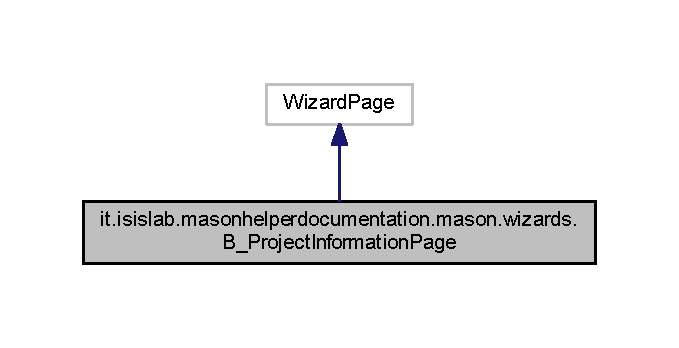
\includegraphics[width=326pt]{classit_1_1isislab_1_1masonhelperdocumentation_1_1mason_1_1wizards_1_1_b___project_information_page__inherit__graph}
\end{center}
\end{figure}


Collaboration diagram for it.\-isislab.\-masonhelperdocumentation.\-mason.\-wizards.\-B\-\_\-\-Project\-Information\-Page\-:
\nopagebreak
\begin{figure}[H]
\begin{center}
\leavevmode
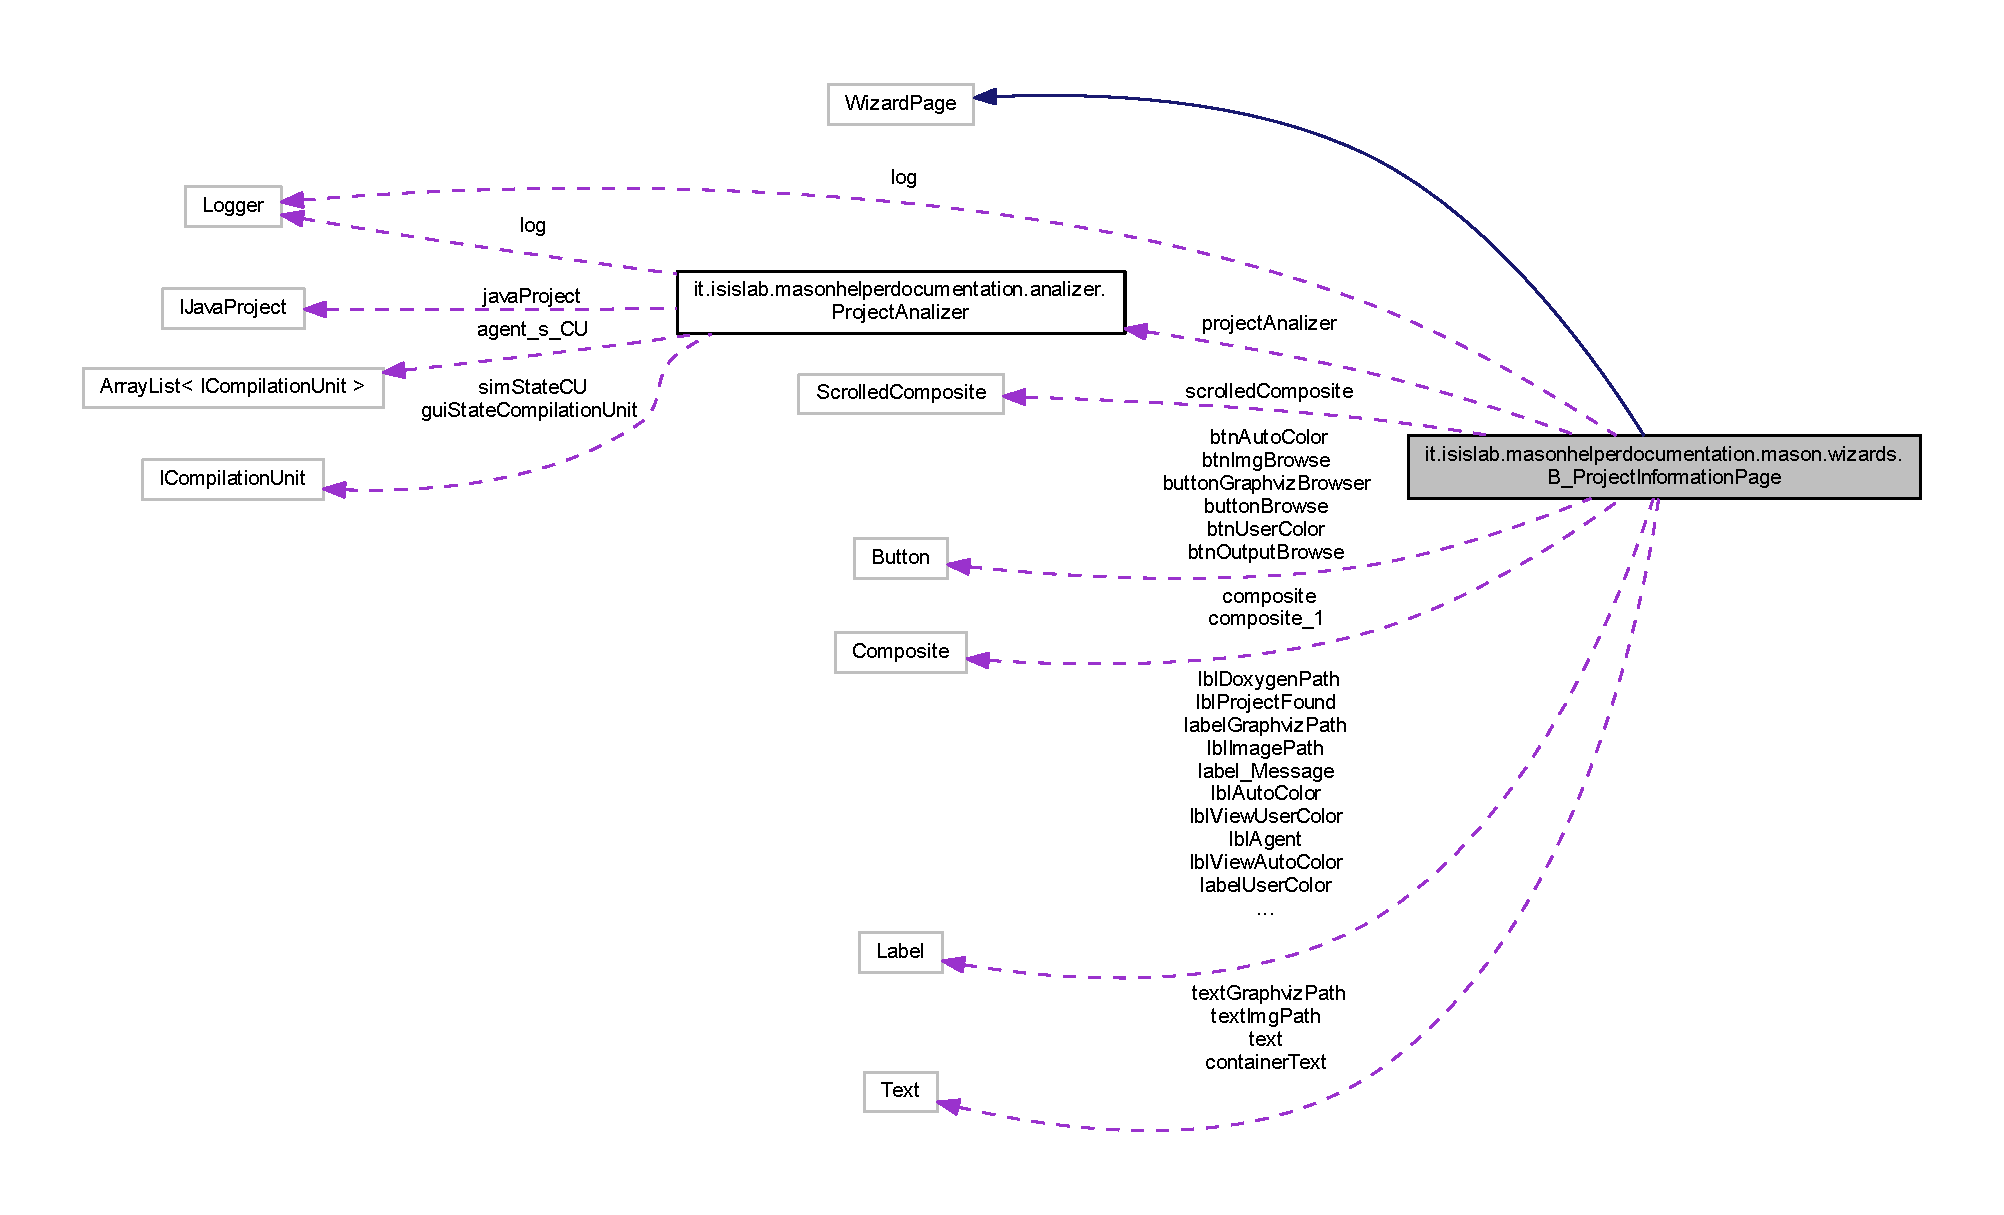
\includegraphics[width=350pt]{classit_1_1isislab_1_1masonhelperdocumentation_1_1mason_1_1wizards_1_1_b___project_information_page__coll__graph}
\end{center}
\end{figure}
\subsection*{Public Member Functions}
\begin{DoxyCompactItemize}
\item 
\hyperlink{classit_1_1isislab_1_1masonhelperdocumentation_1_1mason_1_1wizards_1_1_b___project_information_page_a78007aec142d1094d5954cd3f6ee4f4e}{B\-\_\-\-Project\-Information\-Page} ()
\item 
boolean \hyperlink{classit_1_1isislab_1_1masonhelperdocumentation_1_1mason_1_1wizards_1_1_b___project_information_page_a0eec0bf0cf4211e377555c20f52abdb8}{is\-Doxygen\-Path\-Set} ()
\item 
void \hyperlink{classit_1_1isislab_1_1masonhelperdocumentation_1_1mason_1_1wizards_1_1_b___project_information_page_abca74e3315d231866ce8a6a016dffaa5}{create\-Control} (Composite parent)
\item 
boolean \hyperlink{classit_1_1isislab_1_1masonhelperdocumentation_1_1mason_1_1wizards_1_1_b___project_information_page_af534554cbdceb3c61b1f48b5df4e290c}{can\-Flip\-To\-Next\-Page} ()
\item 
boolean \hyperlink{classit_1_1isislab_1_1masonhelperdocumentation_1_1mason_1_1wizards_1_1_b___project_information_page_a27830e10567ec9e8c2e855b80f07f5ad}{is\-Page\-Complete} ()
\item 
I\-Wizard\-Page \hyperlink{classit_1_1isislab_1_1masonhelperdocumentation_1_1mason_1_1wizards_1_1_b___project_information_page_ac7752ebb107ca9c3a83640a09edce745}{get\-Next\-Page} ()
\end{DoxyCompactItemize}
\subsection*{Private Member Functions}
\begin{DoxyCompactItemize}
\item 
void \hyperlink{classit_1_1isislab_1_1masonhelperdocumentation_1_1mason_1_1wizards_1_1_b___project_information_page_a787830581d3746b970cde68fec9d59b3}{set\-Doxygen\-Label\-Path\-From\-Config} ()
\item 
void \hyperlink{classit_1_1isislab_1_1masonhelperdocumentation_1_1mason_1_1wizards_1_1_b___project_information_page_afa7497cd5a5b4b3c5fb7f7f1397ebb72}{set\-Project\-Label} ()
\end{DoxyCompactItemize}
\subsection*{Private Attributes}
\begin{DoxyCompactItemize}
\item 
Text \hyperlink{classit_1_1isislab_1_1masonhelperdocumentation_1_1mason_1_1wizards_1_1_b___project_information_page_a0951101436c6e108b0dcbea4b8a5cfd7}{container\-Text}
\item 
Label \hyperlink{classit_1_1isislab_1_1masonhelperdocumentation_1_1mason_1_1wizards_1_1_b___project_information_page_a204ffc289609a627b90d6c31b2105c1b}{lbl\-Doxygen\-Path}
\item 
Button \hyperlink{classit_1_1isislab_1_1masonhelperdocumentation_1_1mason_1_1wizards_1_1_b___project_information_page_ac64957cf0d484de5c9aec87db660cfb7}{button\-Browse}
\item 
\hyperlink{classit_1_1isislab_1_1masonhelperdocumentation_1_1analizer_1_1_project_analizer}{Project\-Analizer} \hyperlink{classit_1_1isislab_1_1masonhelperdocumentation_1_1mason_1_1wizards_1_1_b___project_information_page_aa0397b2de6a01a90d6d2eb52645f5173}{project\-Analizer}
\item 
Label \hyperlink{classit_1_1isislab_1_1masonhelperdocumentation_1_1mason_1_1wizards_1_1_b___project_information_page_a36bd57a557296f92577dfd09d585cc52}{lbl\-Image\-Path}
\item 
Text \hyperlink{classit_1_1isislab_1_1masonhelperdocumentation_1_1mason_1_1wizards_1_1_b___project_information_page_a2d8d332de830585ce52efe2c43ff9e2b}{text\-Img\-Path}
\item 
Button \hyperlink{classit_1_1isislab_1_1masonhelperdocumentation_1_1mason_1_1wizards_1_1_b___project_information_page_a0c6e3746265bd68e2ef73050896e03af}{btn\-Img\-Browse}
\item 
Text \hyperlink{classit_1_1isislab_1_1masonhelperdocumentation_1_1mason_1_1wizards_1_1_b___project_information_page_ac62e1a690396a9296b72dda3e66d0a55}{text}
\item 
Button \hyperlink{classit_1_1isislab_1_1masonhelperdocumentation_1_1mason_1_1wizards_1_1_b___project_information_page_ab2605aae4ffe03c9e27ad871c1eab17f}{btn\-Output\-Browse}
\item 
Label \hyperlink{classit_1_1isislab_1_1masonhelperdocumentation_1_1mason_1_1wizards_1_1_b___project_information_page_a57169e3a422df52ec0ade1e68cab1e02}{label\-Graphviz\-Path}
\item 
Text \hyperlink{classit_1_1isislab_1_1masonhelperdocumentation_1_1mason_1_1wizards_1_1_b___project_information_page_a7aefdf9fbb7f43f9b7d2a8175e7128e7}{text\-Graphviz\-Path}
\item 
Button \hyperlink{classit_1_1isislab_1_1masonhelperdocumentation_1_1mason_1_1wizards_1_1_b___project_information_page_ac42d6f27c381517f450b92aff3407d3b}{button\-Graphviz\-Browser}
\item 
Scrolled\-Composite \hyperlink{classit_1_1isislab_1_1masonhelperdocumentation_1_1mason_1_1wizards_1_1_b___project_information_page_aefd8edc54e474960b861b1071734298d}{scrolled\-Composite}
\item 
Composite \hyperlink{classit_1_1isislab_1_1masonhelperdocumentation_1_1mason_1_1wizards_1_1_b___project_information_page_a5463a1c435b5fdb6fc4ca2009d7ed215}{composite}
\item 
Label \hyperlink{classit_1_1isislab_1_1masonhelperdocumentation_1_1mason_1_1wizards_1_1_b___project_information_page_ac69e795f916c2ab72be4bfaa25f6add8}{lbl\-Project\-Found}
\item 
Label \hyperlink{classit_1_1isislab_1_1masonhelperdocumentation_1_1mason_1_1wizards_1_1_b___project_information_page_a28b79fed5c44e30e5616d79b026b612c}{lbl\-Gui\-State}
\item 
Label \hyperlink{classit_1_1isislab_1_1masonhelperdocumentation_1_1mason_1_1wizards_1_1_b___project_information_page_a13dbe5977135d636e30124b11e884870}{lbl\-Sim\-State}
\item 
Label \hyperlink{classit_1_1isislab_1_1masonhelperdocumentation_1_1mason_1_1wizards_1_1_b___project_information_page_a13700876bf889b097f466ac7d3e7128c}{lbl\-Agent}
\item 
Label \hyperlink{classit_1_1isislab_1_1masonhelperdocumentation_1_1mason_1_1wizards_1_1_b___project_information_page_a92c697e221a10de24614780a6bdb2d3a}{label\-\_\-\-Message}
\item 
Composite \hyperlink{classit_1_1isislab_1_1masonhelperdocumentation_1_1mason_1_1wizards_1_1_b___project_information_page_ad2438c6d59f23f0717a1503f4e823bb8}{composite\-\_\-1}
\item 
Button \hyperlink{classit_1_1isislab_1_1masonhelperdocumentation_1_1mason_1_1wizards_1_1_b___project_information_page_a60a4bbca5d0ee37acbc02b31f69db1bd}{btn\-Auto\-Color}
\item 
Label \hyperlink{classit_1_1isislab_1_1masonhelperdocumentation_1_1mason_1_1wizards_1_1_b___project_information_page_a2f300a11970751b92cd1f06b864da746}{lbl\-Auto\-Color}
\item 
Label \hyperlink{classit_1_1isislab_1_1masonhelperdocumentation_1_1mason_1_1wizards_1_1_b___project_information_page_a7b37d666f12fa1c7ea739a7a9878ba9b}{label\-User\-Color}
\item 
Button \hyperlink{classit_1_1isislab_1_1masonhelperdocumentation_1_1mason_1_1wizards_1_1_b___project_information_page_a50713187368f9e3d91689c820090feb2}{btn\-User\-Color}
\item 
Label \hyperlink{classit_1_1isislab_1_1masonhelperdocumentation_1_1mason_1_1wizards_1_1_b___project_information_page_a649e641abf9319f5db69ccf3333fbf41}{lbl\-View\-Auto\-Color}
\item 
Label \hyperlink{classit_1_1isislab_1_1masonhelperdocumentation_1_1mason_1_1wizards_1_1_b___project_information_page_ab1b4ec7a5a8736cf063250290326f061}{lbl\-View\-User\-Color}
\end{DoxyCompactItemize}
\subsection*{Static Private Attributes}
\begin{DoxyCompactItemize}
\item 
static Logger \hyperlink{classit_1_1isislab_1_1masonhelperdocumentation_1_1mason_1_1wizards_1_1_b___project_information_page_a301b0d0144053deada2aaf4e6968003f}{log} = Logger.\-get\-Logger(\char`\"{}global\char`\"{})
\end{DoxyCompactItemize}


\subsection{Detailed Description}
\begin{DoxyAuthor}{Author}
Romano Simone 0512101343 This page show some settings to begin wizard. 
\end{DoxyAuthor}


\subsection{Constructor \& Destructor Documentation}
\hypertarget{classit_1_1isislab_1_1masonhelperdocumentation_1_1mason_1_1wizards_1_1_b___project_information_page_a78007aec142d1094d5954cd3f6ee4f4e}{\index{it\-::isislab\-::masonhelperdocumentation\-::mason\-::wizards\-::\-B\-\_\-\-Project\-Information\-Page@{it\-::isislab\-::masonhelperdocumentation\-::mason\-::wizards\-::\-B\-\_\-\-Project\-Information\-Page}!B\-\_\-\-Project\-Information\-Page@{B\-\_\-\-Project\-Information\-Page}}
\index{B\-\_\-\-Project\-Information\-Page@{B\-\_\-\-Project\-Information\-Page}!it::isislab::masonhelperdocumentation::mason::wizards::B_ProjectInformationPage@{it\-::isislab\-::masonhelperdocumentation\-::mason\-::wizards\-::\-B\-\_\-\-Project\-Information\-Page}}
\subsubsection[{B\-\_\-\-Project\-Information\-Page}]{\setlength{\rightskip}{0pt plus 5cm}it.\-isislab.\-masonhelperdocumentation.\-mason.\-wizards.\-B\-\_\-\-Project\-Information\-Page.\-B\-\_\-\-Project\-Information\-Page (
\begin{DoxyParamCaption}
{}
\end{DoxyParamCaption}
)}}\label{classit_1_1isislab_1_1masonhelperdocumentation_1_1mason_1_1wizards_1_1_b___project_information_page_a78007aec142d1094d5954cd3f6ee4f4e}
Constructor for Page1.


\begin{DoxyParams}{Parameters}
{\em java\-Project} & \\
\hline
\end{DoxyParams}

\begin{DoxyCode}
72                                       \{
73         super(\textcolor{stringliteral}{"wizardPage"});
74         setTitle(\textcolor{stringliteral}{"MASON Helper documentation"});
75         setDescription(\textcolor{stringliteral}{"This wizard will extract a documentation for Simulation model using Doxygen."});
76         \hyperlink{classit_1_1isislab_1_1masonhelperdocumentation_1_1mason_1_1wizards_1_1_b___project_information_page_aa0397b2de6a01a90d6d2eb52645f5173}{projectAnalizer} = GlobalUtility.getProjectAnalizer();
77     \}
\end{DoxyCode}


\subsection{Member Function Documentation}
\hypertarget{classit_1_1isislab_1_1masonhelperdocumentation_1_1mason_1_1wizards_1_1_b___project_information_page_af534554cbdceb3c61b1f48b5df4e290c}{\index{it\-::isislab\-::masonhelperdocumentation\-::mason\-::wizards\-::\-B\-\_\-\-Project\-Information\-Page@{it\-::isislab\-::masonhelperdocumentation\-::mason\-::wizards\-::\-B\-\_\-\-Project\-Information\-Page}!can\-Flip\-To\-Next\-Page@{can\-Flip\-To\-Next\-Page}}
\index{can\-Flip\-To\-Next\-Page@{can\-Flip\-To\-Next\-Page}!it::isislab::masonhelperdocumentation::mason::wizards::B_ProjectInformationPage@{it\-::isislab\-::masonhelperdocumentation\-::mason\-::wizards\-::\-B\-\_\-\-Project\-Information\-Page}}
\subsubsection[{can\-Flip\-To\-Next\-Page}]{\setlength{\rightskip}{0pt plus 5cm}boolean it.\-isislab.\-masonhelperdocumentation.\-mason.\-wizards.\-B\-\_\-\-Project\-Information\-Page.\-can\-Flip\-To\-Next\-Page (
\begin{DoxyParamCaption}
{}
\end{DoxyParamCaption}
)}}\label{classit_1_1isislab_1_1masonhelperdocumentation_1_1mason_1_1wizards_1_1_b___project_information_page_af534554cbdceb3c61b1f48b5df4e290c}

\begin{DoxyCode}
388                                        \{
389         \textcolor{keywordflow}{return} \hyperlink{classit_1_1isislab_1_1masonhelperdocumentation_1_1mason_1_1wizards_1_1_b___project_information_page_a0eec0bf0cf4211e377555c20f52abdb8}{isDoxygenPathSet}() && projectAnalizer.isMasonProject();
390     \}
\end{DoxyCode}


Here is the call graph for this function\-:
\nopagebreak
\begin{figure}[H]
\begin{center}
\leavevmode
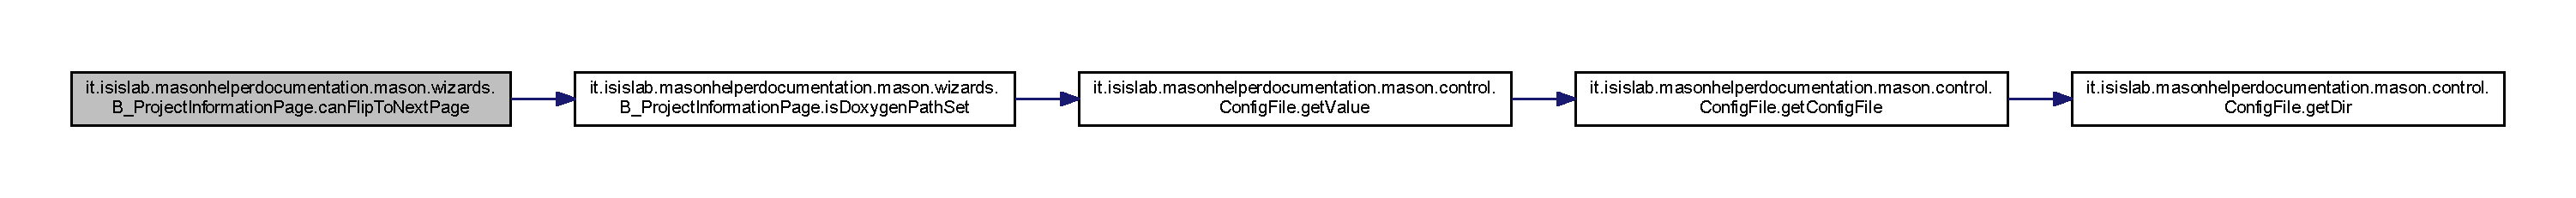
\includegraphics[width=350pt]{classit_1_1isislab_1_1masonhelperdocumentation_1_1mason_1_1wizards_1_1_b___project_information_page_af534554cbdceb3c61b1f48b5df4e290c_cgraph}
\end{center}
\end{figure}




Here is the caller graph for this function\-:
\nopagebreak
\begin{figure}[H]
\begin{center}
\leavevmode
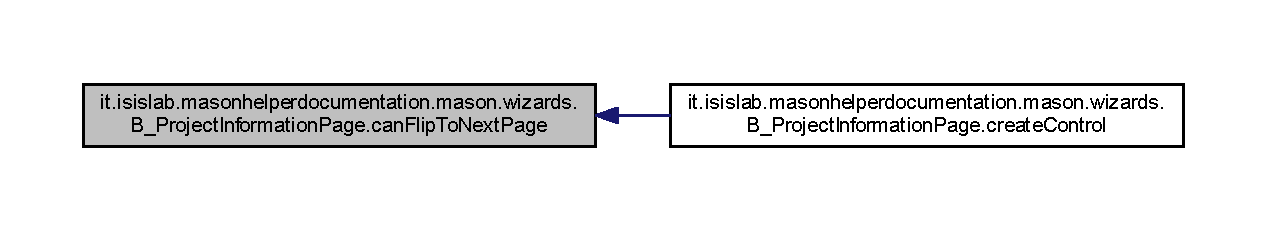
\includegraphics[width=350pt]{classit_1_1isislab_1_1masonhelperdocumentation_1_1mason_1_1wizards_1_1_b___project_information_page_af534554cbdceb3c61b1f48b5df4e290c_icgraph}
\end{center}
\end{figure}


\hypertarget{classit_1_1isislab_1_1masonhelperdocumentation_1_1mason_1_1wizards_1_1_b___project_information_page_abca74e3315d231866ce8a6a016dffaa5}{\index{it\-::isislab\-::masonhelperdocumentation\-::mason\-::wizards\-::\-B\-\_\-\-Project\-Information\-Page@{it\-::isislab\-::masonhelperdocumentation\-::mason\-::wizards\-::\-B\-\_\-\-Project\-Information\-Page}!create\-Control@{create\-Control}}
\index{create\-Control@{create\-Control}!it::isislab::masonhelperdocumentation::mason::wizards::B_ProjectInformationPage@{it\-::isislab\-::masonhelperdocumentation\-::mason\-::wizards\-::\-B\-\_\-\-Project\-Information\-Page}}
\subsubsection[{create\-Control}]{\setlength{\rightskip}{0pt plus 5cm}void it.\-isislab.\-masonhelperdocumentation.\-mason.\-wizards.\-B\-\_\-\-Project\-Information\-Page.\-create\-Control (
\begin{DoxyParamCaption}
\item[{Composite}]{parent}
\end{DoxyParamCaption}
)}}\label{classit_1_1isislab_1_1masonhelperdocumentation_1_1mason_1_1wizards_1_1_b___project_information_page_abca74e3315d231866ce8a6a016dffaa5}

\begin{DoxyCode}
92                                                 \{
93         Composite container = \textcolor{keyword}{new} Composite(parent, SWT.NULL);
94         GridLayout layout = \textcolor{keyword}{new} GridLayout();
95         container.setLayout(layout);
96         layout.numColumns = 3;
97         layout.verticalSpacing = 9;
98         
99         Label lblOutputPath = \textcolor{keyword}{new} Label(container, SWT.NONE);
100         lblOutputPath.setLayoutData(\textcolor{keyword}{new} GridData(SWT.RIGHT, SWT.CENTER, \textcolor{keyword}{false}, \textcolor{keyword}{false}, 1, 1));
101         lblOutputPath.setText(\textcolor{stringliteral}{"Output path:"});
102         
103         \hyperlink{classit_1_1isislab_1_1masonhelperdocumentation_1_1mason_1_1wizards_1_1_b___project_information_page_ac62e1a690396a9296b72dda3e66d0a55}{text} = \textcolor{keyword}{new} Text(container, SWT.BORDER);
104         text.setLayoutData(\textcolor{keyword}{new} GridData(SWT.FILL, SWT.CENTER, \textcolor{keyword}{true}, \textcolor{keyword}{false}, 1, 1));
105         text.setText(ConfigFile.getValue(\textcolor{stringliteral}{"output"}));
106         
107         \hyperlink{classit_1_1isislab_1_1masonhelperdocumentation_1_1mason_1_1wizards_1_1_b___project_information_page_ab2605aae4ffe03c9e27ad871c1eab17f}{btnOutputBrowse} = \textcolor{keyword}{new} Button(container, SWT.NONE);
108         btnOutputBrowse.addSelectionListener(\textcolor{keyword}{new} SelectionAdapter() \{
109             @Override
110             \textcolor{keyword}{public} \textcolor{keywordtype}{void} widgetSelected(SelectionEvent e) \{
111                 JFileChooser chooser = \textcolor{keyword}{new} JFileChooser();
112                 chooser.setCurrentDirectory(\textcolor{keyword}{new} java.io.File(\textcolor{stringliteral}{"."}));
113                 chooser.setDialogTitle(\textcolor{stringliteral}{"Browse the folder to process"});
114                 chooser.setFileSelectionMode(JFileChooser.DIRECTORIES\_ONLY);
115                 chooser.setAcceptAllFileFilterUsed(\textcolor{keyword}{false});
116                 \textcolor{keywordflow}{if} (chooser.showOpenDialog(null) == JFileChooser.APPROVE\_OPTION) \{                         
           
117                     ConfigFile.setProperty(\textcolor{stringliteral}{"output"}, chooser.getSelectedFile().getAbsolutePath());
118                     log.info(\textcolor{stringliteral}{"Config file updated: "} + chooser.getCurrentDirectory().getPath());
119                     text.setText(ConfigFile.getValue(\textcolor{stringliteral}{"output"}));
120                 \}
121             \}
122         \});
123         btnOutputBrowse.setText(\textcolor{stringliteral}{"Browse..."});
124         \hyperlink{classit_1_1isislab_1_1masonhelperdocumentation_1_1mason_1_1wizards_1_1_b___project_information_page_a204ffc289609a627b90d6c31b2105c1b}{lblDoxygenPath} = \textcolor{keyword}{new} Label(container, SWT.NULL);
125         lblDoxygenPath.setLayoutData(\textcolor{keyword}{new} GridData(SWT.RIGHT, SWT.CENTER, \textcolor{keyword}{false}, \textcolor{keyword}{false}, 1, 1));
126         lblDoxygenPath.setText(\textcolor{stringliteral}{"Doxygen path:"});
127 
128         \hyperlink{classit_1_1isislab_1_1masonhelperdocumentation_1_1mason_1_1wizards_1_1_b___project_information_page_a0951101436c6e108b0dcbea4b8a5cfd7}{containerText} = \textcolor{keyword}{new} Text(container, SWT.BORDER | SWT.SINGLE);
129         containerText.setLayoutData(\textcolor{keyword}{new} GridData(GridData.FILL\_HORIZONTAL));
130 
131         \hyperlink{classit_1_1isislab_1_1masonhelperdocumentation_1_1mason_1_1wizards_1_1_b___project_information_page_ac64957cf0d484de5c9aec87db660cfb7}{buttonBrowse} = \textcolor{keyword}{new} Button(container, SWT.PUSH);
132         buttonBrowse.addSelectionListener(\textcolor{keyword}{new} SelectionAdapter() \{
133             @Override
134             \textcolor{keyword}{public} \textcolor{keywordtype}{void} widgetSelected(SelectionEvent e) \{
135                 JFileChooser chooser = \textcolor{keyword}{new} JFileChooser();
136                 chooser.setCurrentDirectory(\textcolor{keyword}{new} java.io.File(\textcolor{stringliteral}{"."}));
137                 chooser.setDialogTitle(\textcolor{stringliteral}{"Browse the folder to process"});
138                 chooser.setFileSelectionMode(JFileChooser.DIRECTORIES\_ONLY);
139                 chooser.setAcceptAllFileFilterUsed(\textcolor{keyword}{false});
140                 \textcolor{keywordflow}{if} (chooser.showOpenDialog(null) == JFileChooser.APPROVE\_OPTION) \{                  
141                     ConfigFile.setProperty(\textcolor{stringliteral}{"doxygenPath"}, chooser.getSelectedFile().getAbsolutePath());
142                     log.info(\textcolor{stringliteral}{"Config file updated: "} + chooser.getCurrentDirectory().getPath());
143                     \hyperlink{classit_1_1isislab_1_1masonhelperdocumentation_1_1mason_1_1wizards_1_1_b___project_information_page_a787830581d3746b970cde68fec9d59b3}{setDoxygenLabelPathFromConfig}();
144                     \hyperlink{classit_1_1isislab_1_1masonhelperdocumentation_1_1mason_1_1wizards_1_1_b___project_information_page_af534554cbdceb3c61b1f48b5df4e290c}{canFlipToNextPage}();
145                 \}
146             \}
147         \});
148         buttonBrowse.setText(\textcolor{stringliteral}{"Browse..."});
149         
150         \hyperlink{classit_1_1isislab_1_1masonhelperdocumentation_1_1mason_1_1wizards_1_1_b___project_information_page_a57169e3a422df52ec0ade1e68cab1e02}{labelGraphvizPath} = \textcolor{keyword}{new} Label(container, SWT.NONE);
151         labelGraphvizPath.setLayoutData(\textcolor{keyword}{new} GridData(SWT.RIGHT, SWT.CENTER, \textcolor{keyword}{false}, \textcolor{keyword}{false}, 1, 1));
152         labelGraphvizPath.setText(\textcolor{stringliteral}{"Graphviz path:"});
153         
154         \hyperlink{classit_1_1isislab_1_1masonhelperdocumentation_1_1mason_1_1wizards_1_1_b___project_information_page_a7aefdf9fbb7f43f9b7d2a8175e7128e7}{textGraphvizPath} = \textcolor{keyword}{new} Text(container, SWT.BORDER);
155         textGraphvizPath.setLayoutData(\textcolor{keyword}{new} GridData(SWT.FILL, SWT.CENTER, \textcolor{keyword}{true}, \textcolor{keyword}{false}, 1, 1));
156         
157         \hyperlink{classit_1_1isislab_1_1masonhelperdocumentation_1_1mason_1_1wizards_1_1_b___project_information_page_ac42d6f27c381517f450b92aff3407d3b}{buttonGraphvizBrowser} = \textcolor{keyword}{new} Button(container, SWT.NONE);
158         buttonGraphvizBrowser.addSelectionListener(\textcolor{keyword}{new} SelectionAdapter() \{
159             @Override
160             \textcolor{keyword}{public} \textcolor{keywordtype}{void} widgetSelected(SelectionEvent e) \{
161                 JFileChooser chooser = \textcolor{keyword}{new} JFileChooser();
162                 chooser.setCurrentDirectory(\textcolor{keyword}{new} java.io.File(\textcolor{stringliteral}{"."}));
163                 chooser.setDialogTitle(\textcolor{stringliteral}{"Browse the folder to process"});
164                 chooser.setFileSelectionMode(JFileChooser.DIRECTORIES\_ONLY);
165                 chooser.setAcceptAllFileFilterUsed(\textcolor{keyword}{false});
166                 \textcolor{keywordflow}{if} (chooser.showOpenDialog(null) == JFileChooser.APPROVE\_OPTION) \{                  
167                     ConfigFile.setProperty(\textcolor{stringliteral}{"graphvizPath"}, chooser.getSelectedFile().getAbsolutePath());
168                     log.info(\textcolor{stringliteral}{"Config file updated: "} + chooser.getCurrentDirectory().getPath());
169                     textGraphvizPath.setText(ConfigFile.getValue(\textcolor{stringliteral}{"graphvizPath"}));
170                     \hyperlink{classit_1_1isislab_1_1masonhelperdocumentation_1_1mason_1_1wizards_1_1_b___project_information_page_af534554cbdceb3c61b1f48b5df4e290c}{canFlipToNextPage}();
171                 \}
172             \}
173         \});
174         buttonGraphvizBrowser.setText(\textcolor{stringliteral}{"Browse..."});
175         textGraphvizPath.setText(ConfigFile.getValue(\textcolor{stringliteral}{"graphvizPath"}));;
176         
177         \hyperlink{classit_1_1isislab_1_1masonhelperdocumentation_1_1mason_1_1wizards_1_1_b___project_information_page_a36bd57a557296f92577dfd09d585cc52}{lblImagePath} = \textcolor{keyword}{new} Label(container, SWT.NONE);
178         lblImagePath.setLayoutData(\textcolor{keyword}{new} GridData(SWT.RIGHT, SWT.CENTER, \textcolor{keyword}{false}, \textcolor{keyword}{false}, 1, 1));
179         lblImagePath.setText(\textcolor{stringliteral}{"Image path:"});
180         
181         \hyperlink{classit_1_1isislab_1_1masonhelperdocumentation_1_1mason_1_1wizards_1_1_b___project_information_page_a2d8d332de830585ce52efe2c43ff9e2b}{textImgPath} = \textcolor{keyword}{new} Text(container, SWT.BORDER);
182         textImgPath.setLayoutData(\textcolor{keyword}{new} GridData(SWT.FILL, SWT.CENTER, \textcolor{keyword}{true}, \textcolor{keyword}{false}, 1, 1));
183         
184         \hyperlink{classit_1_1isislab_1_1masonhelperdocumentation_1_1mason_1_1wizards_1_1_b___project_information_page_a0c6e3746265bd68e2ef73050896e03af}{btnImgBrowse} = \textcolor{keyword}{new} Button(container, SWT.NONE);
185         btnImgBrowse.addSelectionListener(\textcolor{keyword}{new} SelectionAdapter() \{
186             @Override
187             \textcolor{keyword}{public} \textcolor{keywordtype}{void} widgetSelected(SelectionEvent e) \{
188                 JFileChooser chooser = \textcolor{keyword}{new} JFileChooser();
189                 chooser.setCurrentDirectory(\textcolor{keyword}{new} java.io.File(\textcolor{stringliteral}{"."}));
190                 chooser.setDialogTitle(\textcolor{stringliteral}{"Browse the folder to process"});
191                 chooser.setFileSelectionMode(JFileChooser.DIRECTORIES\_ONLY);
192                 chooser.setAcceptAllFileFilterUsed(\textcolor{keyword}{false});
193                 \textcolor{keywordflow}{if} (chooser.showOpenDialog(null) == JFileChooser.APPROVE\_OPTION) \{                  
194                     ConfigFile.setProperty(\textcolor{stringliteral}{"imgPath"}, chooser.getSelectedFile().getAbsolutePath());
195                     log.info(\textcolor{stringliteral}{"Config file updated: "} + chooser.getCurrentDirectory().getPath());
196                     textImgPath.setText(ConfigFile.getValue(\textcolor{stringliteral}{"imgPath"}));
197                 \}
198             \}
199         \});
200         btnImgBrowse.setText(\textcolor{stringliteral}{"Browse..."});
201         textImgPath.setText(ConfigFile.getValue(\textcolor{stringliteral}{"imgPath"}));
202         \textcolor{keyword}{new} Label(container, SWT.NONE);
203         \textcolor{keyword}{new} Label(container, SWT.NONE);
204         \textcolor{keyword}{new} Label(container, SWT.NONE);
205         \textcolor{keyword}{new} Label(container, SWT.NONE);
206         
207         \hyperlink{classit_1_1isislab_1_1masonhelperdocumentation_1_1mason_1_1wizards_1_1_b___project_information_page_ad2438c6d59f23f0717a1503f4e823bb8}{composite\_1} = \textcolor{keyword}{new} Composite(container, SWT.NONE);
208         composite\_1.setLayout(\textcolor{keyword}{new} GridLayout(3, \textcolor{keyword}{false}));
209         GridData gd\_composite\_1 = \textcolor{keyword}{new} GridData(SWT.LEFT, SWT.CENTER, \textcolor{keyword}{false}, \textcolor{keyword}{false}, 1, 1);
210         gd\_composite\_1.widthHint = 401;
211         gd\_composite\_1.heightHint = 60;
212         composite\_1.setLayoutData(gd\_composite\_1);
213         
214         \hyperlink{classit_1_1isislab_1_1masonhelperdocumentation_1_1mason_1_1wizards_1_1_b___project_information_page_a2f300a11970751b92cd1f06b864da746}{lblAutoColor} = \textcolor{keyword}{new} Label(\hyperlink{classit_1_1isislab_1_1masonhelperdocumentation_1_1mason_1_1wizards_1_1_b___project_information_page_ad2438c6d59f23f0717a1503f4e823bb8}{composite\_1}, SWT.NONE);
215         lblAutoColor.setLayoutData(\textcolor{keyword}{new} GridData(SWT.RIGHT, SWT.CENTER, \textcolor{keyword}{false}, \textcolor{keyword}{false}, 1, 1));
216         lblAutoColor.setText(\textcolor{stringliteral}{"Auto-generated info color:"});
217 
218         
219         \textcolor{keyword}{final} RGB autoRGB = \textcolor{keyword}{new} RGB(32, 1, 205);    \textcolor{comment}{//default blue}
220         \textcolor{keywordflow}{if} (!ConfigFile.getValue(\textcolor{stringliteral}{"R\_Value\_auto"}).equals(\textcolor{stringliteral}{""}) && !ConfigFile.getValue(\textcolor{stringliteral}{"G\_Value\_auto"}).equals(\textcolor{stringliteral}{
      ""}) && !ConfigFile.getValue(\textcolor{stringliteral}{"B\_Value\_auto"}).equals(\textcolor{stringliteral}{""}))\{
221             autoRGB.red = Integer.parseInt(ConfigFile.getValue(\textcolor{stringliteral}{"R\_Value\_auto"}));
222             autoRGB.green = Integer.parseInt(ConfigFile.getValue(\textcolor{stringliteral}{"G\_Value\_auto"}));
223             autoRGB.blue = Integer.parseInt(ConfigFile.getValue(\textcolor{stringliteral}{"B\_Value\_auto"}));       
224             GlobalUtility.autoOutputColor[0] = autoRGB.red;
225             GlobalUtility.autoOutputColor[1] = autoRGB.green;
226             GlobalUtility.autoOutputColor[2] = autoRGB.blue;
227         \}
228         \hyperlink{classit_1_1isislab_1_1masonhelperdocumentation_1_1mason_1_1wizards_1_1_b___project_information_page_a60a4bbca5d0ee37acbc02b31f69db1bd}{btnAutoColor} = \textcolor{keyword}{new} Button(\hyperlink{classit_1_1isislab_1_1masonhelperdocumentation_1_1mason_1_1wizards_1_1_b___project_information_page_ad2438c6d59f23f0717a1503f4e823bb8}{composite\_1}, SWT.NONE);
229         btnAutoColor.setText(\textcolor{stringliteral}{"Choose"});
230         \hyperlink{classit_1_1isislab_1_1masonhelperdocumentation_1_1mason_1_1wizards_1_1_b___project_information_page_a649e641abf9319f5db69ccf3333fbf41}{lblViewAutoColor} = \textcolor{keyword}{new} Label(\hyperlink{classit_1_1isislab_1_1masonhelperdocumentation_1_1mason_1_1wizards_1_1_b___project_information_page_ad2438c6d59f23f0717a1503f4e823bb8}{composite\_1}, SWT.NONE);
231         lblViewAutoColor.setForeground(SWTResourceManager.getColor(autoRGB));
232         lblViewAutoColor.setText(\textcolor{stringliteral}{"AAAAA"});
233         lblViewAutoColor.setBackground(SWTResourceManager.getColor(autoRGB));
234         btnAutoColor.addSelectionListener(\textcolor{keyword}{new} SelectionAdapter() \{
235             @Override
236             \textcolor{keyword}{public} \textcolor{keywordtype}{void} widgetSelected(SelectionEvent e) \{
237                 Color c = JColorChooser.showDialog(null, \textcolor{stringliteral}{"Choose a Color"}, null);
238                   \textcolor{keywordflow}{if} (c != null)\{
239                       autoRGB.red = c.getRed();
240                       autoRGB.green = c.getGreen();
241                       autoRGB.blue = c.getBlue();
242                       lblViewAutoColor.setForeground(SWTResourceManager.getColor(autoRGB));
243                       lblViewAutoColor.setBackground(SWTResourceManager.getColor(autoRGB));
244                       GlobalUtility.autoOutputColor[0] = c.getRed();
245                       GlobalUtility.autoOutputColor[1] = c.getGreen();
246                       GlobalUtility.autoOutputColor[2] = c.getBlue();
247                       ConfigFile.setProperty(\textcolor{stringliteral}{"R\_Value\_auto"}, c.getRed()+\textcolor{stringliteral}{""});
248                       ConfigFile.setProperty(\textcolor{stringliteral}{"G\_Value\_auto"}, c.getGreen()+\textcolor{stringliteral}{""});
249                       ConfigFile.setProperty(\textcolor{stringliteral}{"B\_Value\_auto"}, c.getBlue()+\textcolor{stringliteral}{""});
250                   \}
251                 \}
252             \});
253         
254         
255         \hyperlink{classit_1_1isislab_1_1masonhelperdocumentation_1_1mason_1_1wizards_1_1_b___project_information_page_a7b37d666f12fa1c7ea739a7a9878ba9b}{labelUserColor} = \textcolor{keyword}{new} Label(\hyperlink{classit_1_1isislab_1_1masonhelperdocumentation_1_1mason_1_1wizards_1_1_b___project_information_page_ad2438c6d59f23f0717a1503f4e823bb8}{composite\_1}, SWT.RIGHT);
256         labelUserColor.setLayoutData(\textcolor{keyword}{new} GridData(SWT.RIGHT, SWT.CENTER, \textcolor{keyword}{false}, \textcolor{keyword}{false}, 1, 1));
257         labelUserColor.setText(\textcolor{stringliteral}{"User info color:"});
258         
259         \textcolor{keyword}{final} RGB userRGB = \textcolor{keyword}{new} RGB(0, 0, 0);   \textcolor{comment}{//default black}
260         \textcolor{keywordflow}{if} (!ConfigFile.getValue(\textcolor{stringliteral}{"R\_Value\_user"}).equals(\textcolor{stringliteral}{""}) && !ConfigFile.getValue(\textcolor{stringliteral}{"G\_Value\_user"}).equals(\textcolor{stringliteral}{
      ""}) && !ConfigFile.getValue(\textcolor{stringliteral}{"B\_Value\_user"}).equals(\textcolor{stringliteral}{""}))\{
261             userRGB.red = Integer.parseInt(ConfigFile.getValue(\textcolor{stringliteral}{"R\_Value\_user"}));
262             userRGB.green = Integer.parseInt(ConfigFile.getValue(\textcolor{stringliteral}{"G\_Value\_user"}));
263             userRGB.blue = Integer.parseInt(ConfigFile.getValue(\textcolor{stringliteral}{"B\_Value\_user"}));
264             GlobalUtility.userOutputColor[0] = userRGB.red;
265             GlobalUtility.userOutputColor[1] = userRGB.green;
266             GlobalUtility.userOutputColor[2] = userRGB.blue;
267         \}
268         \hyperlink{classit_1_1isislab_1_1masonhelperdocumentation_1_1mason_1_1wizards_1_1_b___project_information_page_a50713187368f9e3d91689c820090feb2}{btnUserColor} = \textcolor{keyword}{new} Button(\hyperlink{classit_1_1isislab_1_1masonhelperdocumentation_1_1mason_1_1wizards_1_1_b___project_information_page_ad2438c6d59f23f0717a1503f4e823bb8}{composite\_1}, SWT.NONE);
269         \hyperlink{classit_1_1isislab_1_1masonhelperdocumentation_1_1mason_1_1wizards_1_1_b___project_information_page_ab1b4ec7a5a8736cf063250290326f061}{lblViewUserColor} = \textcolor{keyword}{new} Label(\hyperlink{classit_1_1isislab_1_1masonhelperdocumentation_1_1mason_1_1wizards_1_1_b___project_information_page_ad2438c6d59f23f0717a1503f4e823bb8}{composite\_1}, SWT.NONE);
270         lblViewUserColor.setText(\textcolor{stringliteral}{"AAAAA"});
271         lblViewUserColor.setForeground(SWTResourceManager.getColor(userRGB));
272         lblViewUserColor.setBackground(SWTResourceManager.getColor(userRGB));
273         btnUserColor.addSelectionListener(\textcolor{keyword}{new} SelectionAdapter() \{
274             @Override
275             \textcolor{keyword}{public} \textcolor{keywordtype}{void} widgetSelected(SelectionEvent e) \{
276                 Color c = JColorChooser.showDialog(null, \textcolor{stringliteral}{"Choose a Color"}, null);
277                   \textcolor{keywordflow}{if} (c != null)\{
278                       userRGB.red = c.getRed();
279                       userRGB.green = c.getGreen();
280                       userRGB.blue = c.getBlue();
281                       lblViewUserColor.setForeground(SWTResourceManager.getColor(userRGB));
282                       lblViewUserColor.setBackground(SWTResourceManager.getColor(userRGB));
283                       GlobalUtility.userOutputColor[0] = c.getRed();
284                       GlobalUtility.userOutputColor[1] = c.getGreen();
285                       GlobalUtility.userOutputColor[2] = c.getBlue();
286                       ConfigFile.setProperty(\textcolor{stringliteral}{"R\_Value\_user"}, c.getRed()+\textcolor{stringliteral}{""});
287                       ConfigFile.setProperty(\textcolor{stringliteral}{"G\_Value\_user"}, c.getGreen()+\textcolor{stringliteral}{""});
288                       ConfigFile.setProperty(\textcolor{stringliteral}{"B\_Value\_user"}, c.getBlue()+\textcolor{stringliteral}{""});
289                   \}
290             \}
291         \});
292         btnUserColor.setText(\textcolor{stringliteral}{"Choose"});
293         
294         
295         \textcolor{keyword}{new} Label(container, SWT.NONE);
296         \textcolor{keyword}{new} Label(container, SWT.NONE);
297         
298         \hyperlink{classit_1_1isislab_1_1masonhelperdocumentation_1_1mason_1_1wizards_1_1_b___project_information_page_a92c697e221a10de24614780a6bdb2d3a}{label\_Message} = \textcolor{keyword}{new} Label(container, SWT.NONE);
299         label\_Message.setText(\textcolor{stringliteral}{""});
300         \textcolor{keyword}{new} Label(container, SWT.NONE);
301         \textcolor{keyword}{new} Label(container, SWT.NONE);
302         
303         \hyperlink{classit_1_1isislab_1_1masonhelperdocumentation_1_1mason_1_1wizards_1_1_b___project_information_page_aefd8edc54e474960b861b1071734298d}{scrolledComposite} = \textcolor{keyword}{new} ScrolledComposite(container, SWT.BORDER | SWT.H\_SCROLL | 
      SWT.V\_SCROLL);
304         GridData gd\_scrolledComposite = \textcolor{keyword}{new} GridData(SWT.LEFT, SWT.CENTER, \textcolor{keyword}{false}, \textcolor{keyword}{false}, 1, 1);
305         gd\_scrolledComposite.heightHint = 75;
306         gd\_scrolledComposite.widthHint = 384;
307         scrolledComposite.setLayoutData(gd\_scrolledComposite);
308         scrolledComposite.setExpandHorizontal(\textcolor{keyword}{true});
309         scrolledComposite.setExpandVertical(\textcolor{keyword}{true});
310         
311         \hyperlink{classit_1_1isislab_1_1masonhelperdocumentation_1_1mason_1_1wizards_1_1_b___project_information_page_a5463a1c435b5fdb6fc4ca2009d7ed215}{composite} = \textcolor{keyword}{new} Composite(\hyperlink{classit_1_1isislab_1_1masonhelperdocumentation_1_1mason_1_1wizards_1_1_b___project_information_page_aefd8edc54e474960b861b1071734298d}{scrolledComposite}, SWT.NONE);
312         composite.setLayout(\textcolor{keyword}{new} GridLayout(1, \textcolor{keyword}{false}));
313         
314         \textcolor{keywordflow}{if} (\hyperlink{classit_1_1isislab_1_1masonhelperdocumentation_1_1mason_1_1wizards_1_1_b___project_information_page_aa0397b2de6a01a90d6d2eb52645f5173}{projectAnalizer}.\hyperlink{classit_1_1isislab_1_1masonhelperdocumentation_1_1analizer_1_1_project_analizer_a57a1bbfb21c09b106d6fa90ad3709d35}{isMasonProject}())\{
315             \hyperlink{classit_1_1isislab_1_1masonhelperdocumentation_1_1mason_1_1wizards_1_1_b___project_information_page_afa7497cd5a5b4b3c5fb7f7f1397ebb72}{setProjectLabel}();
316         \}
317         scrolledComposite.setContent(\hyperlink{classit_1_1isislab_1_1masonhelperdocumentation_1_1mason_1_1wizards_1_1_b___project_information_page_a5463a1c435b5fdb6fc4ca2009d7ed215}{composite});
318         scrolledComposite.setMinSize(composite.computeSize(SWT.DEFAULT, SWT.DEFAULT));
319         \textcolor{keyword}{new} Label(container, SWT.NONE);
320         setControl(container);
321         
322         \hyperlink{classit_1_1isislab_1_1masonhelperdocumentation_1_1mason_1_1wizards_1_1_b___project_information_page_a787830581d3746b970cde68fec9d59b3}{setDoxygenLabelPathFromConfig}();
323         \textcolor{keywordflow}{if} (!\hyperlink{classit_1_1isislab_1_1masonhelperdocumentation_1_1mason_1_1wizards_1_1_b___project_information_page_aa0397b2de6a01a90d6d2eb52645f5173}{projectAnalizer}.\hyperlink{classit_1_1isislab_1_1masonhelperdocumentation_1_1analizer_1_1_project_analizer_a57a1bbfb21c09b106d6fa90ad3709d35}{isMasonProject}()) 
      \hyperlink{classit_1_1isislab_1_1masonhelperdocumentation_1_1mason_1_1wizards_1_1_b___project_information_page_a92c697e221a10de24614780a6bdb2d3a}{label\_Message}.setText(\textcolor{stringliteral}{"Please select a project that use MASON library!"});
324         \textcolor{keywordflow}{if} (\hyperlink{classit_1_1isislab_1_1masonhelperdocumentation_1_1mason_1_1wizards_1_1_b___project_information_page_a0eec0bf0cf4211e377555c20f52abdb8}{isDoxygenPathSet}() && \hyperlink{classit_1_1isislab_1_1masonhelperdocumentation_1_1mason_1_1wizards_1_1_b___project_information_page_aa0397b2de6a01a90d6d2eb52645f5173}{projectAnalizer}.
      \hyperlink{classit_1_1isislab_1_1masonhelperdocumentation_1_1analizer_1_1_project_analizer_a57a1bbfb21c09b106d6fa90ad3709d35}{isMasonProject}()) super.setPageComplete(\textcolor{keyword}{true});
325         \textcolor{keywordflow}{else}    super.setPageComplete(\textcolor{keyword}{false});
326         
327         \textcolor{comment}{//What we can see?}
328         String outputType = ConfigFile.getValue(\textcolor{stringliteral}{"outputType"});
329         \textcolor{keywordflow}{if} (outputType.equals(\textcolor{stringliteral}{"pdf"}))\{
330             lblDoxygenPath.setVisible(\textcolor{keyword}{false});
331             labelGraphvizPath.setVisible(\textcolor{keyword}{false});
332             lblAutoColor.setVisible(\textcolor{keyword}{false});
333             labelUserColor.setVisible(\textcolor{keyword}{false});
334             containerText.setVisible(\textcolor{keyword}{false});
335             textGraphvizPath.setVisible(\textcolor{keyword}{false});
336             btnAutoColor.setVisible(\textcolor{keyword}{false});
337             btnUserColor.setVisible(\textcolor{keyword}{false});
338             buttonBrowse.setVisible(\textcolor{keyword}{false});
339             buttonGraphvizBrowser.setVisible(\textcolor{keyword}{false});
340             lblViewAutoColor.setVisible(\textcolor{keyword}{false});
341             lblViewUserColor.setVisible(\textcolor{keyword}{false});
342         \}
343         \textcolor{keywordflow}{if} (outputType.equals(\textcolor{stringliteral}{"txt"}))\{
344             lblDoxygenPath.setVisible(\textcolor{keyword}{false});
345             labelGraphvizPath.setVisible(\textcolor{keyword}{false});
346             lblAutoColor.setVisible(\textcolor{keyword}{false});
347             labelUserColor.setVisible(\textcolor{keyword}{false});
348             lblImagePath.setVisible(\textcolor{keyword}{false});
349             containerText.setVisible(\textcolor{keyword}{false});
350             textGraphvizPath.setVisible(\textcolor{keyword}{false});
351             textImgPath.setVisible(\textcolor{keyword}{false});
352             btnAutoColor.setVisible(\textcolor{keyword}{false});
353             btnUserColor.setVisible(\textcolor{keyword}{false});
354             btnImgBrowse.setVisible(\textcolor{keyword}{false});
355             buttonBrowse.setVisible(\textcolor{keyword}{false});
356             buttonGraphvizBrowser.setVisible(\textcolor{keyword}{false});
357             lblViewAutoColor.setVisible(\textcolor{keyword}{false});
358             lblViewUserColor.setVisible(\textcolor{keyword}{false});
359         \}   
360     \}
\end{DoxyCode}


Here is the call graph for this function\-:
\nopagebreak
\begin{figure}[H]
\begin{center}
\leavevmode
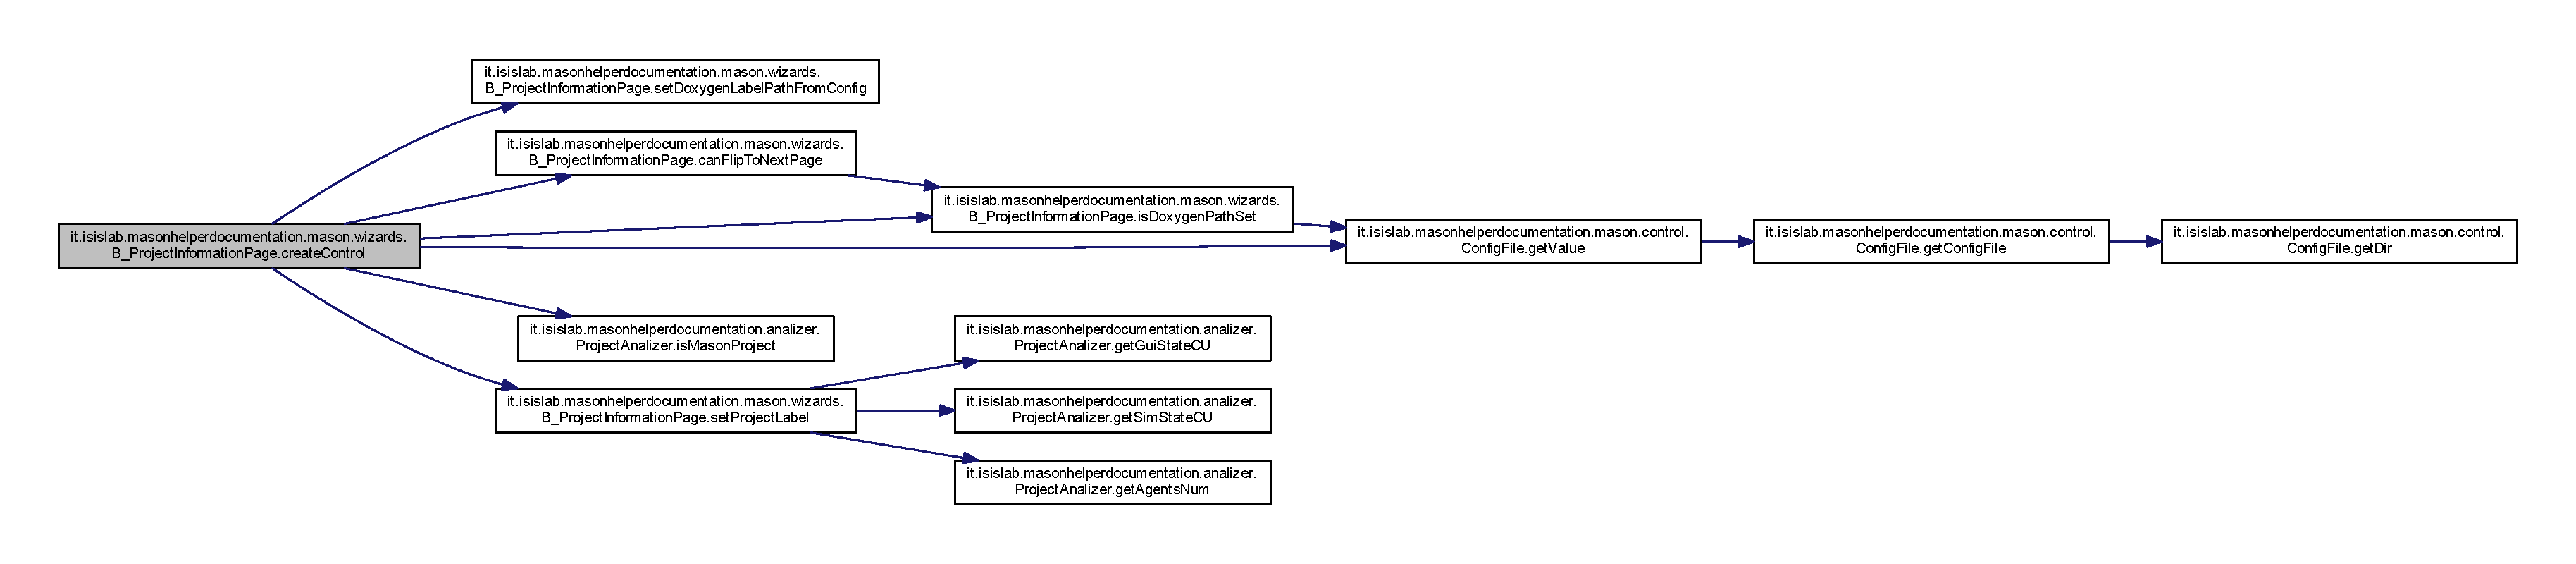
\includegraphics[width=350pt]{classit_1_1isislab_1_1masonhelperdocumentation_1_1mason_1_1wizards_1_1_b___project_information_page_abca74e3315d231866ce8a6a016dffaa5_cgraph}
\end{center}
\end{figure}


\hypertarget{classit_1_1isislab_1_1masonhelperdocumentation_1_1mason_1_1wizards_1_1_b___project_information_page_ac7752ebb107ca9c3a83640a09edce745}{\index{it\-::isislab\-::masonhelperdocumentation\-::mason\-::wizards\-::\-B\-\_\-\-Project\-Information\-Page@{it\-::isislab\-::masonhelperdocumentation\-::mason\-::wizards\-::\-B\-\_\-\-Project\-Information\-Page}!get\-Next\-Page@{get\-Next\-Page}}
\index{get\-Next\-Page@{get\-Next\-Page}!it::isislab::masonhelperdocumentation::mason::wizards::B_ProjectInformationPage@{it\-::isislab\-::masonhelperdocumentation\-::mason\-::wizards\-::\-B\-\_\-\-Project\-Information\-Page}}
\subsubsection[{get\-Next\-Page}]{\setlength{\rightskip}{0pt plus 5cm}I\-Wizard\-Page it.\-isislab.\-masonhelperdocumentation.\-mason.\-wizards.\-B\-\_\-\-Project\-Information\-Page.\-get\-Next\-Page (
\begin{DoxyParamCaption}
{}
\end{DoxyParamCaption}
)}}\label{classit_1_1isislab_1_1masonhelperdocumentation_1_1mason_1_1wizards_1_1_b___project_information_page_ac7752ebb107ca9c3a83640a09edce745}

\begin{DoxyCode}
397                                     \{ 
398         C\_PurposePage nextPage = \textcolor{keyword}{new} C\_PurposePage();
399         ((MASONDocumentationWizard) super.getWizard()).addPage(nextPage);
400         \textcolor{keywordflow}{return} nextPage;
401     \}
\end{DoxyCode}
\hypertarget{classit_1_1isislab_1_1masonhelperdocumentation_1_1mason_1_1wizards_1_1_b___project_information_page_a0eec0bf0cf4211e377555c20f52abdb8}{\index{it\-::isislab\-::masonhelperdocumentation\-::mason\-::wizards\-::\-B\-\_\-\-Project\-Information\-Page@{it\-::isislab\-::masonhelperdocumentation\-::mason\-::wizards\-::\-B\-\_\-\-Project\-Information\-Page}!is\-Doxygen\-Path\-Set@{is\-Doxygen\-Path\-Set}}
\index{is\-Doxygen\-Path\-Set@{is\-Doxygen\-Path\-Set}!it::isislab::masonhelperdocumentation::mason::wizards::B_ProjectInformationPage@{it\-::isislab\-::masonhelperdocumentation\-::mason\-::wizards\-::\-B\-\_\-\-Project\-Information\-Page}}
\subsubsection[{is\-Doxygen\-Path\-Set}]{\setlength{\rightskip}{0pt plus 5cm}boolean it.\-isislab.\-masonhelperdocumentation.\-mason.\-wizards.\-B\-\_\-\-Project\-Information\-Page.\-is\-Doxygen\-Path\-Set (
\begin{DoxyParamCaption}
{}
\end{DoxyParamCaption}
)}}\label{classit_1_1isislab_1_1masonhelperdocumentation_1_1mason_1_1wizards_1_1_b___project_information_page_a0eec0bf0cf4211e377555c20f52abdb8}
Check if Doxygen path is set \begin{DoxyReturn}{Returns}
true if Doxygen path is set 
\end{DoxyReturn}

\begin{DoxyCode}
88                                      \{
89         \textcolor{keywordflow}{return} (ConfigFile.getValue(\textcolor{stringliteral}{"doxygenPath"})!=null);
90     \}
\end{DoxyCode}


Here is the call graph for this function\-:
\nopagebreak
\begin{figure}[H]
\begin{center}
\leavevmode
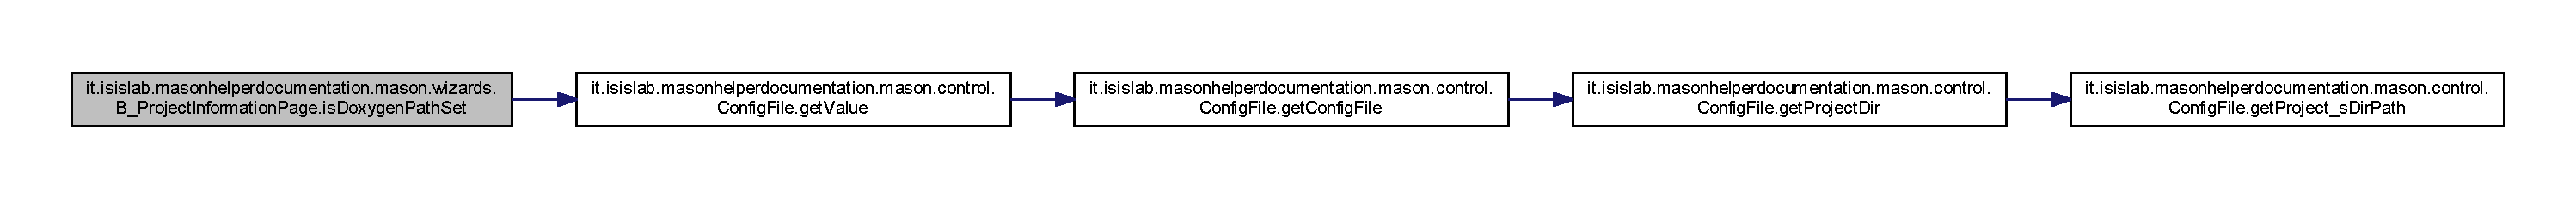
\includegraphics[width=350pt]{classit_1_1isislab_1_1masonhelperdocumentation_1_1mason_1_1wizards_1_1_b___project_information_page_a0eec0bf0cf4211e377555c20f52abdb8_cgraph}
\end{center}
\end{figure}




Here is the caller graph for this function\-:
\nopagebreak
\begin{figure}[H]
\begin{center}
\leavevmode
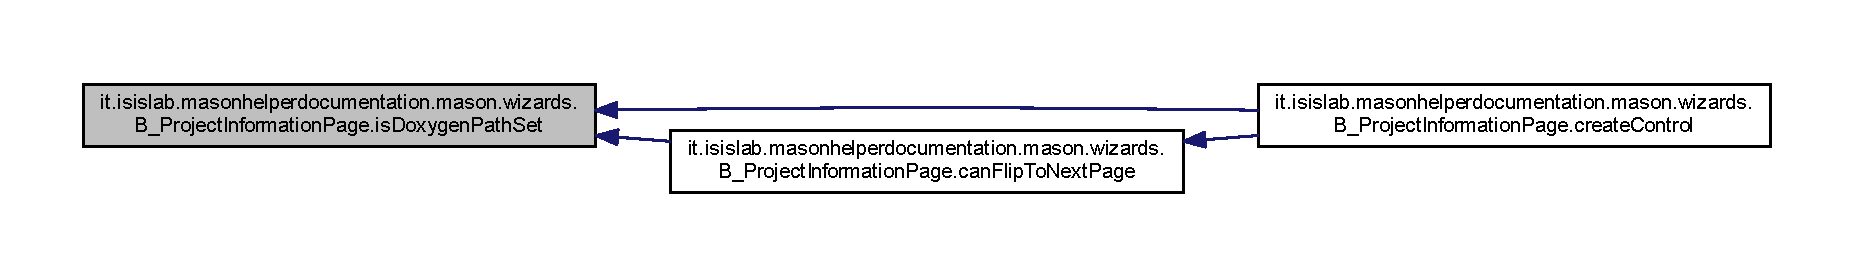
\includegraphics[width=350pt]{classit_1_1isislab_1_1masonhelperdocumentation_1_1mason_1_1wizards_1_1_b___project_information_page_a0eec0bf0cf4211e377555c20f52abdb8_icgraph}
\end{center}
\end{figure}


\hypertarget{classit_1_1isislab_1_1masonhelperdocumentation_1_1mason_1_1wizards_1_1_b___project_information_page_a27830e10567ec9e8c2e855b80f07f5ad}{\index{it\-::isislab\-::masonhelperdocumentation\-::mason\-::wizards\-::\-B\-\_\-\-Project\-Information\-Page@{it\-::isislab\-::masonhelperdocumentation\-::mason\-::wizards\-::\-B\-\_\-\-Project\-Information\-Page}!is\-Page\-Complete@{is\-Page\-Complete}}
\index{is\-Page\-Complete@{is\-Page\-Complete}!it::isislab::masonhelperdocumentation::mason::wizards::B_ProjectInformationPage@{it\-::isislab\-::masonhelperdocumentation\-::mason\-::wizards\-::\-B\-\_\-\-Project\-Information\-Page}}
\subsubsection[{is\-Page\-Complete}]{\setlength{\rightskip}{0pt plus 5cm}boolean it.\-isislab.\-masonhelperdocumentation.\-mason.\-wizards.\-B\-\_\-\-Project\-Information\-Page.\-is\-Page\-Complete (
\begin{DoxyParamCaption}
{}
\end{DoxyParamCaption}
)}}\label{classit_1_1isislab_1_1masonhelperdocumentation_1_1mason_1_1wizards_1_1_b___project_information_page_a27830e10567ec9e8c2e855b80f07f5ad}

\begin{DoxyCode}
393                                    \{
394         \textcolor{keywordflow}{return} \textcolor{keyword}{true};
395     \}
\end{DoxyCode}
\hypertarget{classit_1_1isislab_1_1masonhelperdocumentation_1_1mason_1_1wizards_1_1_b___project_information_page_a787830581d3746b970cde68fec9d59b3}{\index{it\-::isislab\-::masonhelperdocumentation\-::mason\-::wizards\-::\-B\-\_\-\-Project\-Information\-Page@{it\-::isislab\-::masonhelperdocumentation\-::mason\-::wizards\-::\-B\-\_\-\-Project\-Information\-Page}!set\-Doxygen\-Label\-Path\-From\-Config@{set\-Doxygen\-Label\-Path\-From\-Config}}
\index{set\-Doxygen\-Label\-Path\-From\-Config@{set\-Doxygen\-Label\-Path\-From\-Config}!it::isislab::masonhelperdocumentation::mason::wizards::B_ProjectInformationPage@{it\-::isislab\-::masonhelperdocumentation\-::mason\-::wizards\-::\-B\-\_\-\-Project\-Information\-Page}}
\subsubsection[{set\-Doxygen\-Label\-Path\-From\-Config}]{\setlength{\rightskip}{0pt plus 5cm}void it.\-isislab.\-masonhelperdocumentation.\-mason.\-wizards.\-B\-\_\-\-Project\-Information\-Page.\-set\-Doxygen\-Label\-Path\-From\-Config (
\begin{DoxyParamCaption}
{}
\end{DoxyParamCaption}
)\hspace{0.3cm}{\ttfamily [private]}}}\label{classit_1_1isislab_1_1masonhelperdocumentation_1_1mason_1_1wizards_1_1_b___project_information_page_a787830581d3746b970cde68fec9d59b3}

\begin{DoxyCode}
79                                                  \{
80         this.containerText.setText(ConfigFile.getValue(\textcolor{stringliteral}{"doxygenPath"}));
81         log.info(\textcolor{stringliteral}{"doxygenPath text update\(\backslash\)n"} + this.containerText.getText());
82     \}
\end{DoxyCode}


Here is the caller graph for this function\-:
\nopagebreak
\begin{figure}[H]
\begin{center}
\leavevmode
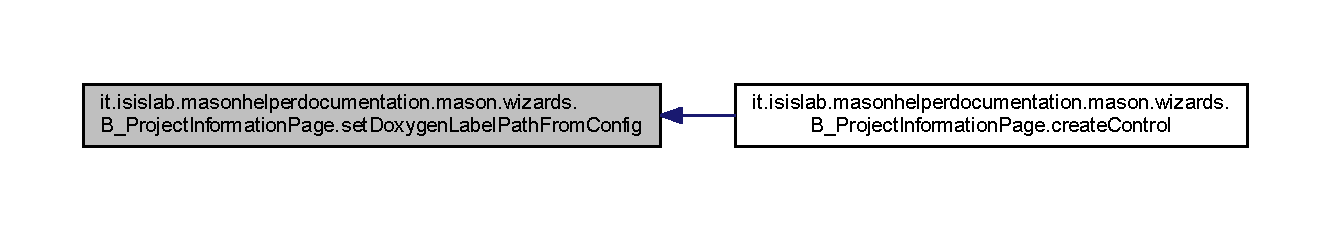
\includegraphics[width=350pt]{classit_1_1isislab_1_1masonhelperdocumentation_1_1mason_1_1wizards_1_1_b___project_information_page_a787830581d3746b970cde68fec9d59b3_icgraph}
\end{center}
\end{figure}


\hypertarget{classit_1_1isislab_1_1masonhelperdocumentation_1_1mason_1_1wizards_1_1_b___project_information_page_afa7497cd5a5b4b3c5fb7f7f1397ebb72}{\index{it\-::isislab\-::masonhelperdocumentation\-::mason\-::wizards\-::\-B\-\_\-\-Project\-Information\-Page@{it\-::isislab\-::masonhelperdocumentation\-::mason\-::wizards\-::\-B\-\_\-\-Project\-Information\-Page}!set\-Project\-Label@{set\-Project\-Label}}
\index{set\-Project\-Label@{set\-Project\-Label}!it::isislab::masonhelperdocumentation::mason::wizards::B_ProjectInformationPage@{it\-::isislab\-::masonhelperdocumentation\-::mason\-::wizards\-::\-B\-\_\-\-Project\-Information\-Page}}
\subsubsection[{set\-Project\-Label}]{\setlength{\rightskip}{0pt plus 5cm}void it.\-isislab.\-masonhelperdocumentation.\-mason.\-wizards.\-B\-\_\-\-Project\-Information\-Page.\-set\-Project\-Label (
\begin{DoxyParamCaption}
{}
\end{DoxyParamCaption}
)\hspace{0.3cm}{\ttfamily [private]}}}\label{classit_1_1isislab_1_1masonhelperdocumentation_1_1mason_1_1wizards_1_1_b___project_information_page_afa7497cd5a5b4b3c5fb7f7f1397ebb72}

\begin{DoxyCode}
362                                    \{
363         \hyperlink{classit_1_1isislab_1_1masonhelperdocumentation_1_1mason_1_1wizards_1_1_b___project_information_page_ac69e795f916c2ab72be4bfaa25f6add8}{lblProjectFound} = \textcolor{keyword}{new} Label(\hyperlink{classit_1_1isislab_1_1masonhelperdocumentation_1_1mason_1_1wizards_1_1_b___project_information_page_a5463a1c435b5fdb6fc4ca2009d7ed215}{composite}, SWT.NONE);
364         lblProjectFound.setText(\textcolor{stringliteral}{"Project Found: "} + projectAnalizer.getProjectName());
365         \textcolor{keywordflow}{if} (\hyperlink{classit_1_1isislab_1_1masonhelperdocumentation_1_1mason_1_1wizards_1_1_b___project_information_page_aa0397b2de6a01a90d6d2eb52645f5173}{projectAnalizer}.\hyperlink{classit_1_1isislab_1_1masonhelperdocumentation_1_1analizer_1_1_project_analizer_afcb9cd776166de6502ac5bff01357457}{getGuiStateCU}()!=null)
366             \textcolor{keywordflow}{if} (\hyperlink{classit_1_1isislab_1_1masonhelperdocumentation_1_1mason_1_1wizards_1_1_b___project_information_page_aa0397b2de6a01a90d6d2eb52645f5173}{projectAnalizer}.\hyperlink{classit_1_1isislab_1_1masonhelperdocumentation_1_1analizer_1_1_project_analizer_afcb9cd776166de6502ac5bff01357457}{getGuiStateCU}().getElementName()!=null)\{
367                 \hyperlink{classit_1_1isislab_1_1masonhelperdocumentation_1_1mason_1_1wizards_1_1_b___project_information_page_a28b79fed5c44e30e5616d79b026b612c}{lblGuiState} = \textcolor{keyword}{new} Label(\hyperlink{classit_1_1isislab_1_1masonhelperdocumentation_1_1mason_1_1wizards_1_1_b___project_information_page_a5463a1c435b5fdb6fc4ca2009d7ed215}{composite}, SWT.NONE);
368                 lblGuiState.setText(\textcolor{stringliteral}{"GUISTATE: "} + projectAnalizer.getGuiStateCU().getElementName());
369             \}
370         \textcolor{keywordflow}{else}
371             lblGuiState.setText(\textcolor{stringliteral}{"GUI not found"});   
372         \hyperlink{classit_1_1isislab_1_1masonhelperdocumentation_1_1mason_1_1wizards_1_1_b___project_information_page_a13dbe5977135d636e30124b11e884870}{lblSimState} = \textcolor{keyword}{new} Label(\hyperlink{classit_1_1isislab_1_1masonhelperdocumentation_1_1mason_1_1wizards_1_1_b___project_information_page_a5463a1c435b5fdb6fc4ca2009d7ed215}{composite}, SWT.NONE);
373         \textcolor{keywordflow}{if} (\hyperlink{classit_1_1isislab_1_1masonhelperdocumentation_1_1mason_1_1wizards_1_1_b___project_information_page_aa0397b2de6a01a90d6d2eb52645f5173}{projectAnalizer}.\hyperlink{classit_1_1isislab_1_1masonhelperdocumentation_1_1analizer_1_1_project_analizer_ab45de2e388d612362f7c79004aa73788}{getSimStateCU}() != null)
374             lblSimState.setText(\textcolor{stringliteral}{"SIMSTATE: "} + \hyperlink{classit_1_1isislab_1_1masonhelperdocumentation_1_1mason_1_1wizards_1_1_b___project_information_page_aa0397b2de6a01a90d6d2eb52645f5173}{projectAnalizer}.
      \hyperlink{classit_1_1isislab_1_1masonhelperdocumentation_1_1analizer_1_1_project_analizer_ab45de2e388d612362f7c79004aa73788}{getSimStateCU}().getElementName());
375         \textcolor{keywordflow}{else}\{
376             JOptionPane.showMessageDialog(null, \textcolor{stringliteral}{"Project doesn't contain SimState Class!"});
377             log.severe(\textcolor{stringliteral}{"Select project doesn't contain SimState Class!"});
378             System.exit(1);;
379         \}           
380         \textcolor{keywordflow}{if} (\hyperlink{classit_1_1isislab_1_1masonhelperdocumentation_1_1mason_1_1wizards_1_1_b___project_information_page_aa0397b2de6a01a90d6d2eb52645f5173}{projectAnalizer}.\hyperlink{classit_1_1isislab_1_1masonhelperdocumentation_1_1analizer_1_1_project_analizer_a48a20f5da4980049099e61b2586ee568}{getAgentsNum}()!=0)\{
381             \hyperlink{classit_1_1isislab_1_1masonhelperdocumentation_1_1mason_1_1wizards_1_1_b___project_information_page_a13700876bf889b097f466ac7d3e7128c}{lblAgent} = \textcolor{keyword}{new} Label(\hyperlink{classit_1_1isislab_1_1masonhelperdocumentation_1_1mason_1_1wizards_1_1_b___project_information_page_a5463a1c435b5fdb6fc4ca2009d7ed215}{composite}, SWT.NONE);
382             \textcolor{keywordflow}{for} (\textcolor{keywordtype}{int} i=0; i<projectAnalizer.getAgentsNum(); i++)
383                 \hyperlink{classit_1_1isislab_1_1masonhelperdocumentation_1_1mason_1_1wizards_1_1_b___project_information_page_a13700876bf889b097f466ac7d3e7128c}{lblAgent}.setText(\hyperlink{classit_1_1isislab_1_1masonhelperdocumentation_1_1mason_1_1wizards_1_1_b___project_information_page_a13700876bf889b097f466ac7d3e7128c}{lblAgent}.getText() + \textcolor{stringliteral}{"AGENT: "} + 
      projectAnalizer.getAgentCU(i).getElementName() +\textcolor{stringliteral}{"\(\backslash\)n"});
384         \}
385     \}
\end{DoxyCode}


Here is the call graph for this function\-:
\nopagebreak
\begin{figure}[H]
\begin{center}
\leavevmode
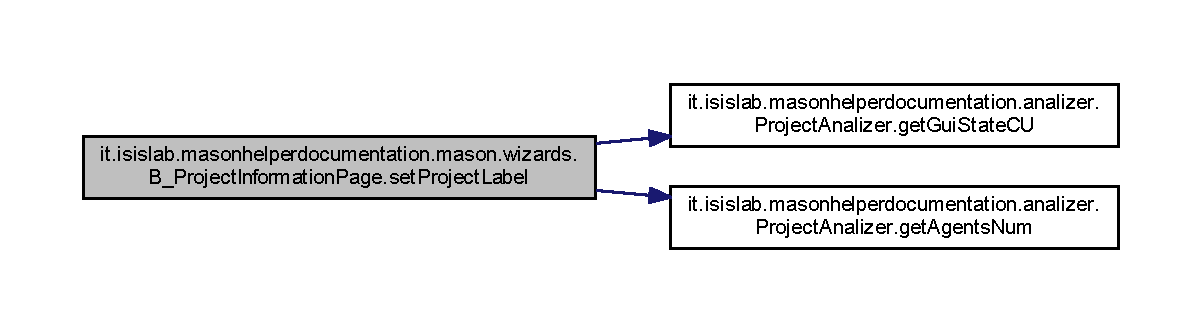
\includegraphics[width=350pt]{classit_1_1isislab_1_1masonhelperdocumentation_1_1mason_1_1wizards_1_1_b___project_information_page_afa7497cd5a5b4b3c5fb7f7f1397ebb72_cgraph}
\end{center}
\end{figure}




Here is the caller graph for this function\-:
\nopagebreak
\begin{figure}[H]
\begin{center}
\leavevmode
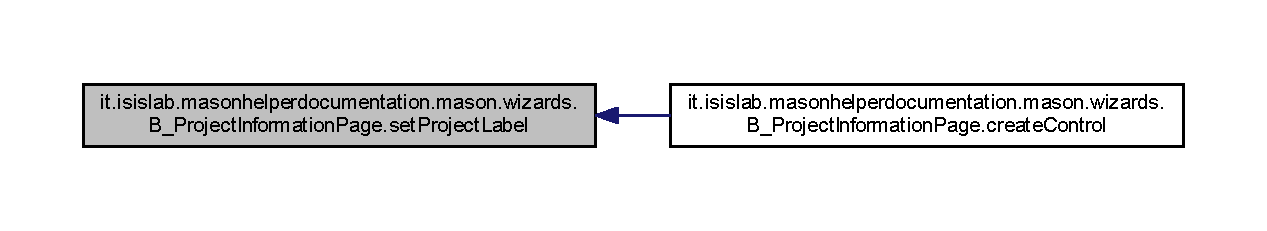
\includegraphics[width=350pt]{classit_1_1isislab_1_1masonhelperdocumentation_1_1mason_1_1wizards_1_1_b___project_information_page_afa7497cd5a5b4b3c5fb7f7f1397ebb72_icgraph}
\end{center}
\end{figure}




\subsection{Member Data Documentation}
\hypertarget{classit_1_1isislab_1_1masonhelperdocumentation_1_1mason_1_1wizards_1_1_b___project_information_page_a60a4bbca5d0ee37acbc02b31f69db1bd}{\index{it\-::isislab\-::masonhelperdocumentation\-::mason\-::wizards\-::\-B\-\_\-\-Project\-Information\-Page@{it\-::isislab\-::masonhelperdocumentation\-::mason\-::wizards\-::\-B\-\_\-\-Project\-Information\-Page}!btn\-Auto\-Color@{btn\-Auto\-Color}}
\index{btn\-Auto\-Color@{btn\-Auto\-Color}!it::isislab::masonhelperdocumentation::mason::wizards::B_ProjectInformationPage@{it\-::isislab\-::masonhelperdocumentation\-::mason\-::wizards\-::\-B\-\_\-\-Project\-Information\-Page}}
\subsubsection[{btn\-Auto\-Color}]{\setlength{\rightskip}{0pt plus 5cm}Button it.\-isislab.\-masonhelperdocumentation.\-mason.\-wizards.\-B\-\_\-\-Project\-Information\-Page.\-btn\-Auto\-Color\hspace{0.3cm}{\ttfamily [private]}}}\label{classit_1_1isislab_1_1masonhelperdocumentation_1_1mason_1_1wizards_1_1_b___project_information_page_a60a4bbca5d0ee37acbc02b31f69db1bd}
\hypertarget{classit_1_1isislab_1_1masonhelperdocumentation_1_1mason_1_1wizards_1_1_b___project_information_page_a0c6e3746265bd68e2ef73050896e03af}{\index{it\-::isislab\-::masonhelperdocumentation\-::mason\-::wizards\-::\-B\-\_\-\-Project\-Information\-Page@{it\-::isislab\-::masonhelperdocumentation\-::mason\-::wizards\-::\-B\-\_\-\-Project\-Information\-Page}!btn\-Img\-Browse@{btn\-Img\-Browse}}
\index{btn\-Img\-Browse@{btn\-Img\-Browse}!it::isislab::masonhelperdocumentation::mason::wizards::B_ProjectInformationPage@{it\-::isislab\-::masonhelperdocumentation\-::mason\-::wizards\-::\-B\-\_\-\-Project\-Information\-Page}}
\subsubsection[{btn\-Img\-Browse}]{\setlength{\rightskip}{0pt plus 5cm}Button it.\-isislab.\-masonhelperdocumentation.\-mason.\-wizards.\-B\-\_\-\-Project\-Information\-Page.\-btn\-Img\-Browse\hspace{0.3cm}{\ttfamily [private]}}}\label{classit_1_1isislab_1_1masonhelperdocumentation_1_1mason_1_1wizards_1_1_b___project_information_page_a0c6e3746265bd68e2ef73050896e03af}
\hypertarget{classit_1_1isislab_1_1masonhelperdocumentation_1_1mason_1_1wizards_1_1_b___project_information_page_ab2605aae4ffe03c9e27ad871c1eab17f}{\index{it\-::isislab\-::masonhelperdocumentation\-::mason\-::wizards\-::\-B\-\_\-\-Project\-Information\-Page@{it\-::isislab\-::masonhelperdocumentation\-::mason\-::wizards\-::\-B\-\_\-\-Project\-Information\-Page}!btn\-Output\-Browse@{btn\-Output\-Browse}}
\index{btn\-Output\-Browse@{btn\-Output\-Browse}!it::isislab::masonhelperdocumentation::mason::wizards::B_ProjectInformationPage@{it\-::isislab\-::masonhelperdocumentation\-::mason\-::wizards\-::\-B\-\_\-\-Project\-Information\-Page}}
\subsubsection[{btn\-Output\-Browse}]{\setlength{\rightskip}{0pt plus 5cm}Button it.\-isislab.\-masonhelperdocumentation.\-mason.\-wizards.\-B\-\_\-\-Project\-Information\-Page.\-btn\-Output\-Browse\hspace{0.3cm}{\ttfamily [private]}}}\label{classit_1_1isislab_1_1masonhelperdocumentation_1_1mason_1_1wizards_1_1_b___project_information_page_ab2605aae4ffe03c9e27ad871c1eab17f}
\hypertarget{classit_1_1isislab_1_1masonhelperdocumentation_1_1mason_1_1wizards_1_1_b___project_information_page_a50713187368f9e3d91689c820090feb2}{\index{it\-::isislab\-::masonhelperdocumentation\-::mason\-::wizards\-::\-B\-\_\-\-Project\-Information\-Page@{it\-::isislab\-::masonhelperdocumentation\-::mason\-::wizards\-::\-B\-\_\-\-Project\-Information\-Page}!btn\-User\-Color@{btn\-User\-Color}}
\index{btn\-User\-Color@{btn\-User\-Color}!it::isislab::masonhelperdocumentation::mason::wizards::B_ProjectInformationPage@{it\-::isislab\-::masonhelperdocumentation\-::mason\-::wizards\-::\-B\-\_\-\-Project\-Information\-Page}}
\subsubsection[{btn\-User\-Color}]{\setlength{\rightskip}{0pt plus 5cm}Button it.\-isislab.\-masonhelperdocumentation.\-mason.\-wizards.\-B\-\_\-\-Project\-Information\-Page.\-btn\-User\-Color\hspace{0.3cm}{\ttfamily [private]}}}\label{classit_1_1isislab_1_1masonhelperdocumentation_1_1mason_1_1wizards_1_1_b___project_information_page_a50713187368f9e3d91689c820090feb2}
\hypertarget{classit_1_1isislab_1_1masonhelperdocumentation_1_1mason_1_1wizards_1_1_b___project_information_page_ac64957cf0d484de5c9aec87db660cfb7}{\index{it\-::isislab\-::masonhelperdocumentation\-::mason\-::wizards\-::\-B\-\_\-\-Project\-Information\-Page@{it\-::isislab\-::masonhelperdocumentation\-::mason\-::wizards\-::\-B\-\_\-\-Project\-Information\-Page}!button\-Browse@{button\-Browse}}
\index{button\-Browse@{button\-Browse}!it::isislab::masonhelperdocumentation::mason::wizards::B_ProjectInformationPage@{it\-::isislab\-::masonhelperdocumentation\-::mason\-::wizards\-::\-B\-\_\-\-Project\-Information\-Page}}
\subsubsection[{button\-Browse}]{\setlength{\rightskip}{0pt plus 5cm}Button it.\-isislab.\-masonhelperdocumentation.\-mason.\-wizards.\-B\-\_\-\-Project\-Information\-Page.\-button\-Browse\hspace{0.3cm}{\ttfamily [private]}}}\label{classit_1_1isislab_1_1masonhelperdocumentation_1_1mason_1_1wizards_1_1_b___project_information_page_ac64957cf0d484de5c9aec87db660cfb7}
\hypertarget{classit_1_1isislab_1_1masonhelperdocumentation_1_1mason_1_1wizards_1_1_b___project_information_page_ac42d6f27c381517f450b92aff3407d3b}{\index{it\-::isislab\-::masonhelperdocumentation\-::mason\-::wizards\-::\-B\-\_\-\-Project\-Information\-Page@{it\-::isislab\-::masonhelperdocumentation\-::mason\-::wizards\-::\-B\-\_\-\-Project\-Information\-Page}!button\-Graphviz\-Browser@{button\-Graphviz\-Browser}}
\index{button\-Graphviz\-Browser@{button\-Graphviz\-Browser}!it::isislab::masonhelperdocumentation::mason::wizards::B_ProjectInformationPage@{it\-::isislab\-::masonhelperdocumentation\-::mason\-::wizards\-::\-B\-\_\-\-Project\-Information\-Page}}
\subsubsection[{button\-Graphviz\-Browser}]{\setlength{\rightskip}{0pt plus 5cm}Button it.\-isislab.\-masonhelperdocumentation.\-mason.\-wizards.\-B\-\_\-\-Project\-Information\-Page.\-button\-Graphviz\-Browser\hspace{0.3cm}{\ttfamily [private]}}}\label{classit_1_1isislab_1_1masonhelperdocumentation_1_1mason_1_1wizards_1_1_b___project_information_page_ac42d6f27c381517f450b92aff3407d3b}
\hypertarget{classit_1_1isislab_1_1masonhelperdocumentation_1_1mason_1_1wizards_1_1_b___project_information_page_a5463a1c435b5fdb6fc4ca2009d7ed215}{\index{it\-::isislab\-::masonhelperdocumentation\-::mason\-::wizards\-::\-B\-\_\-\-Project\-Information\-Page@{it\-::isislab\-::masonhelperdocumentation\-::mason\-::wizards\-::\-B\-\_\-\-Project\-Information\-Page}!composite@{composite}}
\index{composite@{composite}!it::isislab::masonhelperdocumentation::mason::wizards::B_ProjectInformationPage@{it\-::isislab\-::masonhelperdocumentation\-::mason\-::wizards\-::\-B\-\_\-\-Project\-Information\-Page}}
\subsubsection[{composite}]{\setlength{\rightskip}{0pt plus 5cm}Composite it.\-isislab.\-masonhelperdocumentation.\-mason.\-wizards.\-B\-\_\-\-Project\-Information\-Page.\-composite\hspace{0.3cm}{\ttfamily [private]}}}\label{classit_1_1isislab_1_1masonhelperdocumentation_1_1mason_1_1wizards_1_1_b___project_information_page_a5463a1c435b5fdb6fc4ca2009d7ed215}
\hypertarget{classit_1_1isislab_1_1masonhelperdocumentation_1_1mason_1_1wizards_1_1_b___project_information_page_ad2438c6d59f23f0717a1503f4e823bb8}{\index{it\-::isislab\-::masonhelperdocumentation\-::mason\-::wizards\-::\-B\-\_\-\-Project\-Information\-Page@{it\-::isislab\-::masonhelperdocumentation\-::mason\-::wizards\-::\-B\-\_\-\-Project\-Information\-Page}!composite\-\_\-1@{composite\-\_\-1}}
\index{composite\-\_\-1@{composite\-\_\-1}!it::isislab::masonhelperdocumentation::mason::wizards::B_ProjectInformationPage@{it\-::isislab\-::masonhelperdocumentation\-::mason\-::wizards\-::\-B\-\_\-\-Project\-Information\-Page}}
\subsubsection[{composite\-\_\-1}]{\setlength{\rightskip}{0pt plus 5cm}Composite it.\-isislab.\-masonhelperdocumentation.\-mason.\-wizards.\-B\-\_\-\-Project\-Information\-Page.\-composite\-\_\-1\hspace{0.3cm}{\ttfamily [private]}}}\label{classit_1_1isislab_1_1masonhelperdocumentation_1_1mason_1_1wizards_1_1_b___project_information_page_ad2438c6d59f23f0717a1503f4e823bb8}
\hypertarget{classit_1_1isislab_1_1masonhelperdocumentation_1_1mason_1_1wizards_1_1_b___project_information_page_a0951101436c6e108b0dcbea4b8a5cfd7}{\index{it\-::isislab\-::masonhelperdocumentation\-::mason\-::wizards\-::\-B\-\_\-\-Project\-Information\-Page@{it\-::isislab\-::masonhelperdocumentation\-::mason\-::wizards\-::\-B\-\_\-\-Project\-Information\-Page}!container\-Text@{container\-Text}}
\index{container\-Text@{container\-Text}!it::isislab::masonhelperdocumentation::mason::wizards::B_ProjectInformationPage@{it\-::isislab\-::masonhelperdocumentation\-::mason\-::wizards\-::\-B\-\_\-\-Project\-Information\-Page}}
\subsubsection[{container\-Text}]{\setlength{\rightskip}{0pt plus 5cm}Text it.\-isislab.\-masonhelperdocumentation.\-mason.\-wizards.\-B\-\_\-\-Project\-Information\-Page.\-container\-Text\hspace{0.3cm}{\ttfamily [private]}}}\label{classit_1_1isislab_1_1masonhelperdocumentation_1_1mason_1_1wizards_1_1_b___project_information_page_a0951101436c6e108b0dcbea4b8a5cfd7}
\hypertarget{classit_1_1isislab_1_1masonhelperdocumentation_1_1mason_1_1wizards_1_1_b___project_information_page_a92c697e221a10de24614780a6bdb2d3a}{\index{it\-::isislab\-::masonhelperdocumentation\-::mason\-::wizards\-::\-B\-\_\-\-Project\-Information\-Page@{it\-::isislab\-::masonhelperdocumentation\-::mason\-::wizards\-::\-B\-\_\-\-Project\-Information\-Page}!label\-\_\-\-Message@{label\-\_\-\-Message}}
\index{label\-\_\-\-Message@{label\-\_\-\-Message}!it::isislab::masonhelperdocumentation::mason::wizards::B_ProjectInformationPage@{it\-::isislab\-::masonhelperdocumentation\-::mason\-::wizards\-::\-B\-\_\-\-Project\-Information\-Page}}
\subsubsection[{label\-\_\-\-Message}]{\setlength{\rightskip}{0pt plus 5cm}Label it.\-isislab.\-masonhelperdocumentation.\-mason.\-wizards.\-B\-\_\-\-Project\-Information\-Page.\-label\-\_\-\-Message\hspace{0.3cm}{\ttfamily [private]}}}\label{classit_1_1isislab_1_1masonhelperdocumentation_1_1mason_1_1wizards_1_1_b___project_information_page_a92c697e221a10de24614780a6bdb2d3a}
\hypertarget{classit_1_1isislab_1_1masonhelperdocumentation_1_1mason_1_1wizards_1_1_b___project_information_page_a57169e3a422df52ec0ade1e68cab1e02}{\index{it\-::isislab\-::masonhelperdocumentation\-::mason\-::wizards\-::\-B\-\_\-\-Project\-Information\-Page@{it\-::isislab\-::masonhelperdocumentation\-::mason\-::wizards\-::\-B\-\_\-\-Project\-Information\-Page}!label\-Graphviz\-Path@{label\-Graphviz\-Path}}
\index{label\-Graphviz\-Path@{label\-Graphviz\-Path}!it::isislab::masonhelperdocumentation::mason::wizards::B_ProjectInformationPage@{it\-::isislab\-::masonhelperdocumentation\-::mason\-::wizards\-::\-B\-\_\-\-Project\-Information\-Page}}
\subsubsection[{label\-Graphviz\-Path}]{\setlength{\rightskip}{0pt plus 5cm}Label it.\-isislab.\-masonhelperdocumentation.\-mason.\-wizards.\-B\-\_\-\-Project\-Information\-Page.\-label\-Graphviz\-Path\hspace{0.3cm}{\ttfamily [private]}}}\label{classit_1_1isislab_1_1masonhelperdocumentation_1_1mason_1_1wizards_1_1_b___project_information_page_a57169e3a422df52ec0ade1e68cab1e02}
\hypertarget{classit_1_1isislab_1_1masonhelperdocumentation_1_1mason_1_1wizards_1_1_b___project_information_page_a7b37d666f12fa1c7ea739a7a9878ba9b}{\index{it\-::isislab\-::masonhelperdocumentation\-::mason\-::wizards\-::\-B\-\_\-\-Project\-Information\-Page@{it\-::isislab\-::masonhelperdocumentation\-::mason\-::wizards\-::\-B\-\_\-\-Project\-Information\-Page}!label\-User\-Color@{label\-User\-Color}}
\index{label\-User\-Color@{label\-User\-Color}!it::isislab::masonhelperdocumentation::mason::wizards::B_ProjectInformationPage@{it\-::isislab\-::masonhelperdocumentation\-::mason\-::wizards\-::\-B\-\_\-\-Project\-Information\-Page}}
\subsubsection[{label\-User\-Color}]{\setlength{\rightskip}{0pt plus 5cm}Label it.\-isislab.\-masonhelperdocumentation.\-mason.\-wizards.\-B\-\_\-\-Project\-Information\-Page.\-label\-User\-Color\hspace{0.3cm}{\ttfamily [private]}}}\label{classit_1_1isislab_1_1masonhelperdocumentation_1_1mason_1_1wizards_1_1_b___project_information_page_a7b37d666f12fa1c7ea739a7a9878ba9b}
\hypertarget{classit_1_1isislab_1_1masonhelperdocumentation_1_1mason_1_1wizards_1_1_b___project_information_page_a13700876bf889b097f466ac7d3e7128c}{\index{it\-::isislab\-::masonhelperdocumentation\-::mason\-::wizards\-::\-B\-\_\-\-Project\-Information\-Page@{it\-::isislab\-::masonhelperdocumentation\-::mason\-::wizards\-::\-B\-\_\-\-Project\-Information\-Page}!lbl\-Agent@{lbl\-Agent}}
\index{lbl\-Agent@{lbl\-Agent}!it::isislab::masonhelperdocumentation::mason::wizards::B_ProjectInformationPage@{it\-::isislab\-::masonhelperdocumentation\-::mason\-::wizards\-::\-B\-\_\-\-Project\-Information\-Page}}
\subsubsection[{lbl\-Agent}]{\setlength{\rightskip}{0pt plus 5cm}Label it.\-isislab.\-masonhelperdocumentation.\-mason.\-wizards.\-B\-\_\-\-Project\-Information\-Page.\-lbl\-Agent\hspace{0.3cm}{\ttfamily [private]}}}\label{classit_1_1isislab_1_1masonhelperdocumentation_1_1mason_1_1wizards_1_1_b___project_information_page_a13700876bf889b097f466ac7d3e7128c}
\hypertarget{classit_1_1isislab_1_1masonhelperdocumentation_1_1mason_1_1wizards_1_1_b___project_information_page_a2f300a11970751b92cd1f06b864da746}{\index{it\-::isislab\-::masonhelperdocumentation\-::mason\-::wizards\-::\-B\-\_\-\-Project\-Information\-Page@{it\-::isislab\-::masonhelperdocumentation\-::mason\-::wizards\-::\-B\-\_\-\-Project\-Information\-Page}!lbl\-Auto\-Color@{lbl\-Auto\-Color}}
\index{lbl\-Auto\-Color@{lbl\-Auto\-Color}!it::isislab::masonhelperdocumentation::mason::wizards::B_ProjectInformationPage@{it\-::isislab\-::masonhelperdocumentation\-::mason\-::wizards\-::\-B\-\_\-\-Project\-Information\-Page}}
\subsubsection[{lbl\-Auto\-Color}]{\setlength{\rightskip}{0pt plus 5cm}Label it.\-isislab.\-masonhelperdocumentation.\-mason.\-wizards.\-B\-\_\-\-Project\-Information\-Page.\-lbl\-Auto\-Color\hspace{0.3cm}{\ttfamily [private]}}}\label{classit_1_1isislab_1_1masonhelperdocumentation_1_1mason_1_1wizards_1_1_b___project_information_page_a2f300a11970751b92cd1f06b864da746}
\hypertarget{classit_1_1isislab_1_1masonhelperdocumentation_1_1mason_1_1wizards_1_1_b___project_information_page_a204ffc289609a627b90d6c31b2105c1b}{\index{it\-::isislab\-::masonhelperdocumentation\-::mason\-::wizards\-::\-B\-\_\-\-Project\-Information\-Page@{it\-::isislab\-::masonhelperdocumentation\-::mason\-::wizards\-::\-B\-\_\-\-Project\-Information\-Page}!lbl\-Doxygen\-Path@{lbl\-Doxygen\-Path}}
\index{lbl\-Doxygen\-Path@{lbl\-Doxygen\-Path}!it::isislab::masonhelperdocumentation::mason::wizards::B_ProjectInformationPage@{it\-::isislab\-::masonhelperdocumentation\-::mason\-::wizards\-::\-B\-\_\-\-Project\-Information\-Page}}
\subsubsection[{lbl\-Doxygen\-Path}]{\setlength{\rightskip}{0pt plus 5cm}Label it.\-isislab.\-masonhelperdocumentation.\-mason.\-wizards.\-B\-\_\-\-Project\-Information\-Page.\-lbl\-Doxygen\-Path\hspace{0.3cm}{\ttfamily [private]}}}\label{classit_1_1isislab_1_1masonhelperdocumentation_1_1mason_1_1wizards_1_1_b___project_information_page_a204ffc289609a627b90d6c31b2105c1b}
\hypertarget{classit_1_1isislab_1_1masonhelperdocumentation_1_1mason_1_1wizards_1_1_b___project_information_page_a28b79fed5c44e30e5616d79b026b612c}{\index{it\-::isislab\-::masonhelperdocumentation\-::mason\-::wizards\-::\-B\-\_\-\-Project\-Information\-Page@{it\-::isislab\-::masonhelperdocumentation\-::mason\-::wizards\-::\-B\-\_\-\-Project\-Information\-Page}!lbl\-Gui\-State@{lbl\-Gui\-State}}
\index{lbl\-Gui\-State@{lbl\-Gui\-State}!it::isislab::masonhelperdocumentation::mason::wizards::B_ProjectInformationPage@{it\-::isislab\-::masonhelperdocumentation\-::mason\-::wizards\-::\-B\-\_\-\-Project\-Information\-Page}}
\subsubsection[{lbl\-Gui\-State}]{\setlength{\rightskip}{0pt plus 5cm}Label it.\-isislab.\-masonhelperdocumentation.\-mason.\-wizards.\-B\-\_\-\-Project\-Information\-Page.\-lbl\-Gui\-State\hspace{0.3cm}{\ttfamily [private]}}}\label{classit_1_1isislab_1_1masonhelperdocumentation_1_1mason_1_1wizards_1_1_b___project_information_page_a28b79fed5c44e30e5616d79b026b612c}
\hypertarget{classit_1_1isislab_1_1masonhelperdocumentation_1_1mason_1_1wizards_1_1_b___project_information_page_a36bd57a557296f92577dfd09d585cc52}{\index{it\-::isislab\-::masonhelperdocumentation\-::mason\-::wizards\-::\-B\-\_\-\-Project\-Information\-Page@{it\-::isislab\-::masonhelperdocumentation\-::mason\-::wizards\-::\-B\-\_\-\-Project\-Information\-Page}!lbl\-Image\-Path@{lbl\-Image\-Path}}
\index{lbl\-Image\-Path@{lbl\-Image\-Path}!it::isislab::masonhelperdocumentation::mason::wizards::B_ProjectInformationPage@{it\-::isislab\-::masonhelperdocumentation\-::mason\-::wizards\-::\-B\-\_\-\-Project\-Information\-Page}}
\subsubsection[{lbl\-Image\-Path}]{\setlength{\rightskip}{0pt plus 5cm}Label it.\-isislab.\-masonhelperdocumentation.\-mason.\-wizards.\-B\-\_\-\-Project\-Information\-Page.\-lbl\-Image\-Path\hspace{0.3cm}{\ttfamily [private]}}}\label{classit_1_1isislab_1_1masonhelperdocumentation_1_1mason_1_1wizards_1_1_b___project_information_page_a36bd57a557296f92577dfd09d585cc52}
\hypertarget{classit_1_1isislab_1_1masonhelperdocumentation_1_1mason_1_1wizards_1_1_b___project_information_page_ac69e795f916c2ab72be4bfaa25f6add8}{\index{it\-::isislab\-::masonhelperdocumentation\-::mason\-::wizards\-::\-B\-\_\-\-Project\-Information\-Page@{it\-::isislab\-::masonhelperdocumentation\-::mason\-::wizards\-::\-B\-\_\-\-Project\-Information\-Page}!lbl\-Project\-Found@{lbl\-Project\-Found}}
\index{lbl\-Project\-Found@{lbl\-Project\-Found}!it::isislab::masonhelperdocumentation::mason::wizards::B_ProjectInformationPage@{it\-::isislab\-::masonhelperdocumentation\-::mason\-::wizards\-::\-B\-\_\-\-Project\-Information\-Page}}
\subsubsection[{lbl\-Project\-Found}]{\setlength{\rightskip}{0pt plus 5cm}Label it.\-isislab.\-masonhelperdocumentation.\-mason.\-wizards.\-B\-\_\-\-Project\-Information\-Page.\-lbl\-Project\-Found\hspace{0.3cm}{\ttfamily [private]}}}\label{classit_1_1isislab_1_1masonhelperdocumentation_1_1mason_1_1wizards_1_1_b___project_information_page_ac69e795f916c2ab72be4bfaa25f6add8}
\hypertarget{classit_1_1isislab_1_1masonhelperdocumentation_1_1mason_1_1wizards_1_1_b___project_information_page_a13dbe5977135d636e30124b11e884870}{\index{it\-::isislab\-::masonhelperdocumentation\-::mason\-::wizards\-::\-B\-\_\-\-Project\-Information\-Page@{it\-::isislab\-::masonhelperdocumentation\-::mason\-::wizards\-::\-B\-\_\-\-Project\-Information\-Page}!lbl\-Sim\-State@{lbl\-Sim\-State}}
\index{lbl\-Sim\-State@{lbl\-Sim\-State}!it::isislab::masonhelperdocumentation::mason::wizards::B_ProjectInformationPage@{it\-::isislab\-::masonhelperdocumentation\-::mason\-::wizards\-::\-B\-\_\-\-Project\-Information\-Page}}
\subsubsection[{lbl\-Sim\-State}]{\setlength{\rightskip}{0pt plus 5cm}Label it.\-isislab.\-masonhelperdocumentation.\-mason.\-wizards.\-B\-\_\-\-Project\-Information\-Page.\-lbl\-Sim\-State\hspace{0.3cm}{\ttfamily [private]}}}\label{classit_1_1isislab_1_1masonhelperdocumentation_1_1mason_1_1wizards_1_1_b___project_information_page_a13dbe5977135d636e30124b11e884870}
\hypertarget{classit_1_1isislab_1_1masonhelperdocumentation_1_1mason_1_1wizards_1_1_b___project_information_page_a649e641abf9319f5db69ccf3333fbf41}{\index{it\-::isislab\-::masonhelperdocumentation\-::mason\-::wizards\-::\-B\-\_\-\-Project\-Information\-Page@{it\-::isislab\-::masonhelperdocumentation\-::mason\-::wizards\-::\-B\-\_\-\-Project\-Information\-Page}!lbl\-View\-Auto\-Color@{lbl\-View\-Auto\-Color}}
\index{lbl\-View\-Auto\-Color@{lbl\-View\-Auto\-Color}!it::isislab::masonhelperdocumentation::mason::wizards::B_ProjectInformationPage@{it\-::isislab\-::masonhelperdocumentation\-::mason\-::wizards\-::\-B\-\_\-\-Project\-Information\-Page}}
\subsubsection[{lbl\-View\-Auto\-Color}]{\setlength{\rightskip}{0pt plus 5cm}Label it.\-isislab.\-masonhelperdocumentation.\-mason.\-wizards.\-B\-\_\-\-Project\-Information\-Page.\-lbl\-View\-Auto\-Color\hspace{0.3cm}{\ttfamily [private]}}}\label{classit_1_1isislab_1_1masonhelperdocumentation_1_1mason_1_1wizards_1_1_b___project_information_page_a649e641abf9319f5db69ccf3333fbf41}
\hypertarget{classit_1_1isislab_1_1masonhelperdocumentation_1_1mason_1_1wizards_1_1_b___project_information_page_ab1b4ec7a5a8736cf063250290326f061}{\index{it\-::isislab\-::masonhelperdocumentation\-::mason\-::wizards\-::\-B\-\_\-\-Project\-Information\-Page@{it\-::isislab\-::masonhelperdocumentation\-::mason\-::wizards\-::\-B\-\_\-\-Project\-Information\-Page}!lbl\-View\-User\-Color@{lbl\-View\-User\-Color}}
\index{lbl\-View\-User\-Color@{lbl\-View\-User\-Color}!it::isislab::masonhelperdocumentation::mason::wizards::B_ProjectInformationPage@{it\-::isislab\-::masonhelperdocumentation\-::mason\-::wizards\-::\-B\-\_\-\-Project\-Information\-Page}}
\subsubsection[{lbl\-View\-User\-Color}]{\setlength{\rightskip}{0pt plus 5cm}Label it.\-isislab.\-masonhelperdocumentation.\-mason.\-wizards.\-B\-\_\-\-Project\-Information\-Page.\-lbl\-View\-User\-Color\hspace{0.3cm}{\ttfamily [private]}}}\label{classit_1_1isislab_1_1masonhelperdocumentation_1_1mason_1_1wizards_1_1_b___project_information_page_ab1b4ec7a5a8736cf063250290326f061}
\hypertarget{classit_1_1isislab_1_1masonhelperdocumentation_1_1mason_1_1wizards_1_1_b___project_information_page_a301b0d0144053deada2aaf4e6968003f}{\index{it\-::isislab\-::masonhelperdocumentation\-::mason\-::wizards\-::\-B\-\_\-\-Project\-Information\-Page@{it\-::isislab\-::masonhelperdocumentation\-::mason\-::wizards\-::\-B\-\_\-\-Project\-Information\-Page}!log@{log}}
\index{log@{log}!it::isislab::masonhelperdocumentation::mason::wizards::B_ProjectInformationPage@{it\-::isislab\-::masonhelperdocumentation\-::mason\-::wizards\-::\-B\-\_\-\-Project\-Information\-Page}}
\subsubsection[{log}]{\setlength{\rightskip}{0pt plus 5cm}Logger it.\-isislab.\-masonhelperdocumentation.\-mason.\-wizards.\-B\-\_\-\-Project\-Information\-Page.\-log = Logger.\-get\-Logger(\char`\"{}global\char`\"{})\hspace{0.3cm}{\ttfamily [static]}, {\ttfamily [private]}}}\label{classit_1_1isislab_1_1masonhelperdocumentation_1_1mason_1_1wizards_1_1_b___project_information_page_a301b0d0144053deada2aaf4e6968003f}
\hypertarget{classit_1_1isislab_1_1masonhelperdocumentation_1_1mason_1_1wizards_1_1_b___project_information_page_aa0397b2de6a01a90d6d2eb52645f5173}{\index{it\-::isislab\-::masonhelperdocumentation\-::mason\-::wizards\-::\-B\-\_\-\-Project\-Information\-Page@{it\-::isislab\-::masonhelperdocumentation\-::mason\-::wizards\-::\-B\-\_\-\-Project\-Information\-Page}!project\-Analizer@{project\-Analizer}}
\index{project\-Analizer@{project\-Analizer}!it::isislab::masonhelperdocumentation::mason::wizards::B_ProjectInformationPage@{it\-::isislab\-::masonhelperdocumentation\-::mason\-::wizards\-::\-B\-\_\-\-Project\-Information\-Page}}
\subsubsection[{project\-Analizer}]{\setlength{\rightskip}{0pt plus 5cm}{\bf Project\-Analizer} it.\-isislab.\-masonhelperdocumentation.\-mason.\-wizards.\-B\-\_\-\-Project\-Information\-Page.\-project\-Analizer\hspace{0.3cm}{\ttfamily [private]}}}\label{classit_1_1isislab_1_1masonhelperdocumentation_1_1mason_1_1wizards_1_1_b___project_information_page_aa0397b2de6a01a90d6d2eb52645f5173}
\hypertarget{classit_1_1isislab_1_1masonhelperdocumentation_1_1mason_1_1wizards_1_1_b___project_information_page_aefd8edc54e474960b861b1071734298d}{\index{it\-::isislab\-::masonhelperdocumentation\-::mason\-::wizards\-::\-B\-\_\-\-Project\-Information\-Page@{it\-::isislab\-::masonhelperdocumentation\-::mason\-::wizards\-::\-B\-\_\-\-Project\-Information\-Page}!scrolled\-Composite@{scrolled\-Composite}}
\index{scrolled\-Composite@{scrolled\-Composite}!it::isislab::masonhelperdocumentation::mason::wizards::B_ProjectInformationPage@{it\-::isislab\-::masonhelperdocumentation\-::mason\-::wizards\-::\-B\-\_\-\-Project\-Information\-Page}}
\subsubsection[{scrolled\-Composite}]{\setlength{\rightskip}{0pt plus 5cm}Scrolled\-Composite it.\-isislab.\-masonhelperdocumentation.\-mason.\-wizards.\-B\-\_\-\-Project\-Information\-Page.\-scrolled\-Composite\hspace{0.3cm}{\ttfamily [private]}}}\label{classit_1_1isislab_1_1masonhelperdocumentation_1_1mason_1_1wizards_1_1_b___project_information_page_aefd8edc54e474960b861b1071734298d}
\hypertarget{classit_1_1isislab_1_1masonhelperdocumentation_1_1mason_1_1wizards_1_1_b___project_information_page_ac62e1a690396a9296b72dda3e66d0a55}{\index{it\-::isislab\-::masonhelperdocumentation\-::mason\-::wizards\-::\-B\-\_\-\-Project\-Information\-Page@{it\-::isislab\-::masonhelperdocumentation\-::mason\-::wizards\-::\-B\-\_\-\-Project\-Information\-Page}!text@{text}}
\index{text@{text}!it::isislab::masonhelperdocumentation::mason::wizards::B_ProjectInformationPage@{it\-::isislab\-::masonhelperdocumentation\-::mason\-::wizards\-::\-B\-\_\-\-Project\-Information\-Page}}
\subsubsection[{text}]{\setlength{\rightskip}{0pt plus 5cm}Text it.\-isislab.\-masonhelperdocumentation.\-mason.\-wizards.\-B\-\_\-\-Project\-Information\-Page.\-text\hspace{0.3cm}{\ttfamily [private]}}}\label{classit_1_1isislab_1_1masonhelperdocumentation_1_1mason_1_1wizards_1_1_b___project_information_page_ac62e1a690396a9296b72dda3e66d0a55}
\hypertarget{classit_1_1isislab_1_1masonhelperdocumentation_1_1mason_1_1wizards_1_1_b___project_information_page_a7aefdf9fbb7f43f9b7d2a8175e7128e7}{\index{it\-::isislab\-::masonhelperdocumentation\-::mason\-::wizards\-::\-B\-\_\-\-Project\-Information\-Page@{it\-::isislab\-::masonhelperdocumentation\-::mason\-::wizards\-::\-B\-\_\-\-Project\-Information\-Page}!text\-Graphviz\-Path@{text\-Graphviz\-Path}}
\index{text\-Graphviz\-Path@{text\-Graphviz\-Path}!it::isislab::masonhelperdocumentation::mason::wizards::B_ProjectInformationPage@{it\-::isislab\-::masonhelperdocumentation\-::mason\-::wizards\-::\-B\-\_\-\-Project\-Information\-Page}}
\subsubsection[{text\-Graphviz\-Path}]{\setlength{\rightskip}{0pt plus 5cm}Text it.\-isislab.\-masonhelperdocumentation.\-mason.\-wizards.\-B\-\_\-\-Project\-Information\-Page.\-text\-Graphviz\-Path\hspace{0.3cm}{\ttfamily [private]}}}\label{classit_1_1isislab_1_1masonhelperdocumentation_1_1mason_1_1wizards_1_1_b___project_information_page_a7aefdf9fbb7f43f9b7d2a8175e7128e7}
\hypertarget{classit_1_1isislab_1_1masonhelperdocumentation_1_1mason_1_1wizards_1_1_b___project_information_page_a2d8d332de830585ce52efe2c43ff9e2b}{\index{it\-::isislab\-::masonhelperdocumentation\-::mason\-::wizards\-::\-B\-\_\-\-Project\-Information\-Page@{it\-::isislab\-::masonhelperdocumentation\-::mason\-::wizards\-::\-B\-\_\-\-Project\-Information\-Page}!text\-Img\-Path@{text\-Img\-Path}}
\index{text\-Img\-Path@{text\-Img\-Path}!it::isislab::masonhelperdocumentation::mason::wizards::B_ProjectInformationPage@{it\-::isislab\-::masonhelperdocumentation\-::mason\-::wizards\-::\-B\-\_\-\-Project\-Information\-Page}}
\subsubsection[{text\-Img\-Path}]{\setlength{\rightskip}{0pt plus 5cm}Text it.\-isislab.\-masonhelperdocumentation.\-mason.\-wizards.\-B\-\_\-\-Project\-Information\-Page.\-text\-Img\-Path\hspace{0.3cm}{\ttfamily [private]}}}\label{classit_1_1isislab_1_1masonhelperdocumentation_1_1mason_1_1wizards_1_1_b___project_information_page_a2d8d332de830585ce52efe2c43ff9e2b}


The documentation for this class was generated from the following file\-:\begin{DoxyCompactItemize}
\item 
src/it/isislab/masonhelperdocumentation/mason/wizards/\hyperlink{_b___project_information_page_8java}{B\-\_\-\-Project\-Information\-Page.\-java}\end{DoxyCompactItemize}

\hypertarget{classit_1_1isislab_1_1masonhelperdocumentation_1_1mason_1_1wizards_1_1_c___purpose_page}{\section{it.\-isislab.\-masonhelperdocumentation.\-mason.\-wizards.\-C\-\_\-\-Purpose\-Page Class Reference}
\label{classit_1_1isislab_1_1masonhelperdocumentation_1_1mason_1_1wizards_1_1_c___purpose_page}\index{it.\-isislab.\-masonhelperdocumentation.\-mason.\-wizards.\-C\-\_\-\-Purpose\-Page@{it.\-isislab.\-masonhelperdocumentation.\-mason.\-wizards.\-C\-\_\-\-Purpose\-Page}}
}


Inheritance diagram for it.\-isislab.\-masonhelperdocumentation.\-mason.\-wizards.\-C\-\_\-\-Purpose\-Page\-:\nopagebreak
\begin{figure}[H]
\begin{center}
\leavevmode
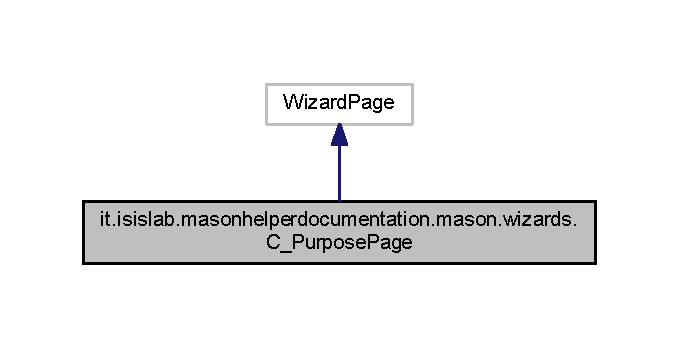
\includegraphics[width=326pt]{classit_1_1isislab_1_1masonhelperdocumentation_1_1mason_1_1wizards_1_1_c___purpose_page__inherit__graph}
\end{center}
\end{figure}


Collaboration diagram for it.\-isislab.\-masonhelperdocumentation.\-mason.\-wizards.\-C\-\_\-\-Purpose\-Page\-:\nopagebreak
\begin{figure}[H]
\begin{center}
\leavevmode
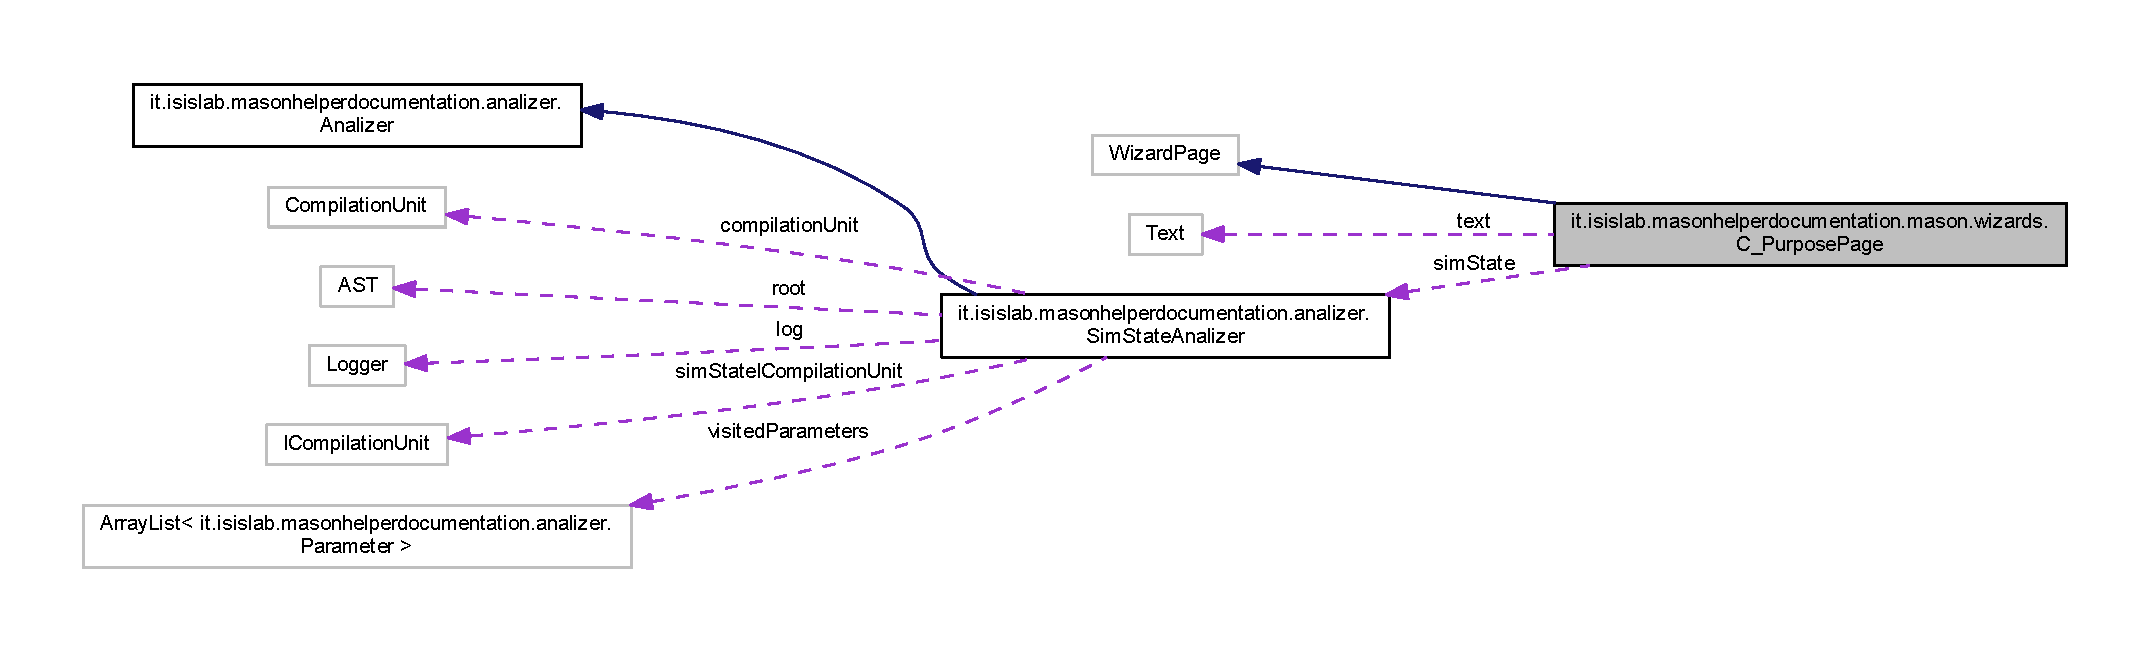
\includegraphics[width=350pt]{classit_1_1isislab_1_1masonhelperdocumentation_1_1mason_1_1wizards_1_1_c___purpose_page__coll__graph}
\end{center}
\end{figure}
\subsection*{Public Member Functions}
\begin{DoxyCompactItemize}
\item 
\hyperlink{classit_1_1isislab_1_1masonhelperdocumentation_1_1mason_1_1wizards_1_1_c___purpose_page_a1c03f292ba0afb1b2be5dd26f8cd3035}{C\-\_\-\-Purpose\-Page} ()
\item 
void \hyperlink{classit_1_1isislab_1_1masonhelperdocumentation_1_1mason_1_1wizards_1_1_c___purpose_page_a735f845063e27f169ea0481efe337aa7}{create\-Control} (Composite parent)
\item 
I\-Wizard\-Page \hyperlink{classit_1_1isislab_1_1masonhelperdocumentation_1_1mason_1_1wizards_1_1_c___purpose_page_ab720ad0f2b4d6f2276b8cc4deaa83d0d}{get\-Next\-Page} ()
\end{DoxyCompactItemize}
\subsection*{Private Member Functions}
\begin{DoxyCompactItemize}
\item 
void \hyperlink{classit_1_1isislab_1_1masonhelperdocumentation_1_1mason_1_1wizards_1_1_c___purpose_page_acb3c2b59b784cc1d761a9d95b5300bb8}{get\-Old\-Information} ()
\end{DoxyCompactItemize}
\subsection*{Private Attributes}
\begin{DoxyCompactItemize}
\item 
Text \hyperlink{classit_1_1isislab_1_1masonhelperdocumentation_1_1mason_1_1wizards_1_1_c___purpose_page_abeec86a6fae75f2a485faeade141dd81}{text}
\item 
\hyperlink{classit_1_1isislab_1_1masonhelperdocumentation_1_1analizer_1_1_sim_state_analizer}{Sim\-State\-Analizer} \hyperlink{classit_1_1isislab_1_1masonhelperdocumentation_1_1mason_1_1wizards_1_1_c___purpose_page_a8441e960f1ba3f3315168635e8976822}{sim\-State}
\end{DoxyCompactItemize}
\subsection*{Static Private Attributes}
\begin{DoxyCompactItemize}
\item 
static String \hyperlink{classit_1_1isislab_1_1masonhelperdocumentation_1_1mason_1_1wizards_1_1_c___purpose_page_a1e19f349d9008f860de96a145f5ea5e7}{page\-Description} = \char`\"{}What is the purpose of the model?\char`\"{}
\end{DoxyCompactItemize}


\subsection{Constructor \& Destructor Documentation}
\hypertarget{classit_1_1isislab_1_1masonhelperdocumentation_1_1mason_1_1wizards_1_1_c___purpose_page_a1c03f292ba0afb1b2be5dd26f8cd3035}{\index{it\-::isislab\-::masonhelperdocumentation\-::mason\-::wizards\-::\-C\-\_\-\-Purpose\-Page@{it\-::isislab\-::masonhelperdocumentation\-::mason\-::wizards\-::\-C\-\_\-\-Purpose\-Page}!C\-\_\-\-Purpose\-Page@{C\-\_\-\-Purpose\-Page}}
\index{C\-\_\-\-Purpose\-Page@{C\-\_\-\-Purpose\-Page}!it::isislab::masonhelperdocumentation::mason::wizards::C_PurposePage@{it\-::isislab\-::masonhelperdocumentation\-::mason\-::wizards\-::\-C\-\_\-\-Purpose\-Page}}
\subsubsection[{C\-\_\-\-Purpose\-Page}]{\setlength{\rightskip}{0pt plus 5cm}it.\-isislab.\-masonhelperdocumentation.\-mason.\-wizards.\-C\-\_\-\-Purpose\-Page.\-C\-\_\-\-Purpose\-Page (
\begin{DoxyParamCaption}
{}
\end{DoxyParamCaption}
)}}\label{classit_1_1isislab_1_1masonhelperdocumentation_1_1mason_1_1wizards_1_1_c___purpose_page_a1c03f292ba0afb1b2be5dd26f8cd3035}

\begin{DoxyCode}
24                            \{
25         super(\textcolor{stringliteral}{"wizardPage"});
26         setTitle(\textcolor{stringliteral}{"1/7 - Purpose"});
27         setDescription(\hyperlink{classit_1_1isislab_1_1masonhelperdocumentation_1_1mason_1_1wizards_1_1_c___purpose_page_a1e19f349d9008f860de96a145f5ea5e7}{pageDescription});
28         \hyperlink{classit_1_1isislab_1_1masonhelperdocumentation_1_1mason_1_1wizards_1_1_c___purpose_page_a8441e960f1ba3f3315168635e8976822}{simState} = GlobalUtility.getSimStateAnalizer();
29     \}
\end{DoxyCode}


\subsection{Member Function Documentation}
\hypertarget{classit_1_1isislab_1_1masonhelperdocumentation_1_1mason_1_1wizards_1_1_c___purpose_page_a735f845063e27f169ea0481efe337aa7}{\index{it\-::isislab\-::masonhelperdocumentation\-::mason\-::wizards\-::\-C\-\_\-\-Purpose\-Page@{it\-::isislab\-::masonhelperdocumentation\-::mason\-::wizards\-::\-C\-\_\-\-Purpose\-Page}!create\-Control@{create\-Control}}
\index{create\-Control@{create\-Control}!it::isislab::masonhelperdocumentation::mason::wizards::C_PurposePage@{it\-::isislab\-::masonhelperdocumentation\-::mason\-::wizards\-::\-C\-\_\-\-Purpose\-Page}}
\subsubsection[{create\-Control}]{\setlength{\rightskip}{0pt plus 5cm}void it.\-isislab.\-masonhelperdocumentation.\-mason.\-wizards.\-C\-\_\-\-Purpose\-Page.\-create\-Control (
\begin{DoxyParamCaption}
\item[{Composite}]{parent}
\end{DoxyParamCaption}
)}}\label{classit_1_1isislab_1_1masonhelperdocumentation_1_1mason_1_1wizards_1_1_c___purpose_page_a735f845063e27f169ea0481efe337aa7}

\begin{DoxyCode}
31                                                 \{
32         Composite container = \textcolor{keyword}{new} Composite(parent, SWT.NULL);
33         setControl(container);
34         container.setLayout(\textcolor{keyword}{new} GridLayout(1, \textcolor{keyword}{false}));      
35         
36         ScrolledComposite scrolledComposite = \textcolor{keyword}{new} ScrolledComposite(container, SWT.BORDER | SWT.H\_SCROLL | 
      SWT.V\_SCROLL);
37         scrolledComposite.setExpandHorizontal(\textcolor{keyword}{true});
38         scrolledComposite.setExpandVertical(\textcolor{keyword}{true});
39         
40         Composite composite = \textcolor{keyword}{new} Composite(scrolledComposite, SWT.NONE);
41         \hyperlink{classit_1_1isislab_1_1masonhelperdocumentation_1_1mason_1_1wizards_1_1_c___purpose_page_abeec86a6fae75f2a485faeade141dd81}{text} = \textcolor{keyword}{new} Text(composite, SWT.BORDER | SWT.H\_SCROLL | SWT.V\_SCROLL | SWT.CANCEL | SWT.MULTI);
42         text.setLocation(0, 0);
43         text.setSize(562, 269);
44         scrolledComposite.setContent(composite);
45         scrolledComposite.setMinSize(composite.computeSize(SWT.DEFAULT, SWT.DEFAULT));
46         \hyperlink{classit_1_1isislab_1_1masonhelperdocumentation_1_1mason_1_1wizards_1_1_c___purpose_page_acb3c2b59b784cc1d761a9d95b5300bb8}{getOldInformation}();
47     \}
\end{DoxyCode}


Here is the call graph for this function\-:\nopagebreak
\begin{figure}[H]
\begin{center}
\leavevmode
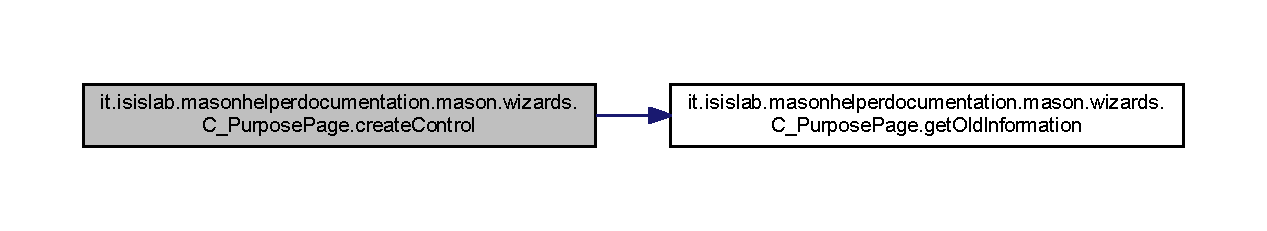
\includegraphics[width=350pt]{classit_1_1isislab_1_1masonhelperdocumentation_1_1mason_1_1wizards_1_1_c___purpose_page_a735f845063e27f169ea0481efe337aa7_cgraph}
\end{center}
\end{figure}


\hypertarget{classit_1_1isislab_1_1masonhelperdocumentation_1_1mason_1_1wizards_1_1_c___purpose_page_ab720ad0f2b4d6f2276b8cc4deaa83d0d}{\index{it\-::isislab\-::masonhelperdocumentation\-::mason\-::wizards\-::\-C\-\_\-\-Purpose\-Page@{it\-::isislab\-::masonhelperdocumentation\-::mason\-::wizards\-::\-C\-\_\-\-Purpose\-Page}!get\-Next\-Page@{get\-Next\-Page}}
\index{get\-Next\-Page@{get\-Next\-Page}!it::isislab::masonhelperdocumentation::mason::wizards::C_PurposePage@{it\-::isislab\-::masonhelperdocumentation\-::mason\-::wizards\-::\-C\-\_\-\-Purpose\-Page}}
\subsubsection[{get\-Next\-Page}]{\setlength{\rightskip}{0pt plus 5cm}I\-Wizard\-Page it.\-isislab.\-masonhelperdocumentation.\-mason.\-wizards.\-C\-\_\-\-Purpose\-Page.\-get\-Next\-Page (
\begin{DoxyParamCaption}
{}
\end{DoxyParamCaption}
)}}\label{classit_1_1isislab_1_1masonhelperdocumentation_1_1mason_1_1wizards_1_1_c___purpose_page_ab720ad0f2b4d6f2276b8cc4deaa83d0d}

\begin{DoxyCode}
56                                     \{ 
57         \textcolor{comment}{//******store information******//}
58         ODD.getPurpose().setModelPurpose(\hyperlink{classit_1_1isislab_1_1masonhelperdocumentation_1_1mason_1_1wizards_1_1_c___purpose_page_abeec86a6fae75f2a485faeade141dd81}{text}.getText());
59         \textcolor{comment}{//****selecting right page****//}
60         \textcolor{keywordflow}{if} (GlobalUtility.getAgentAnalizer() != null)\{
61             D\_AgentDescriptionPage nextPage = \textcolor{keyword}{new} D\_AgentDescriptionPage();
62             ((MASONDocumentationWizard) super.getWizard()).addPage(nextPage);
63             \textcolor{keywordflow}{return} nextPage;
64         \}
65         \textcolor{keywordflow}{else}\{
66             G\_GridsCellPage nextPage = \textcolor{keyword}{new} G\_GridsCellPage();
67             ((MASONDocumentationWizard) super.getWizard()).addPage(nextPage);
68             \textcolor{keywordflow}{return} nextPage;
69         \}
70     \}
\end{DoxyCode}


Here is the call graph for this function\-:\nopagebreak
\begin{figure}[H]
\begin{center}
\leavevmode
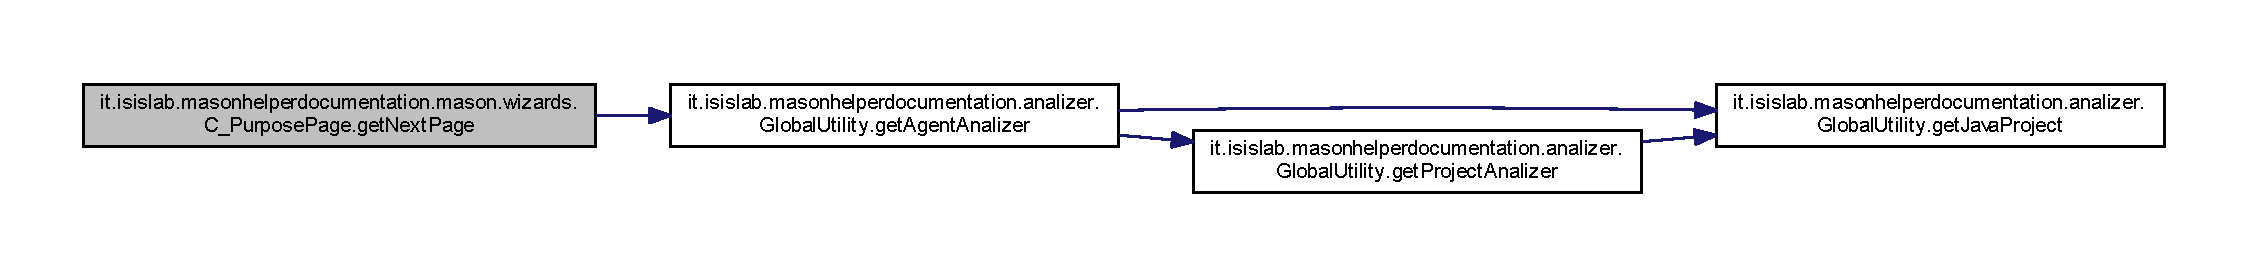
\includegraphics[width=350pt]{classit_1_1isislab_1_1masonhelperdocumentation_1_1mason_1_1wizards_1_1_c___purpose_page_ab720ad0f2b4d6f2276b8cc4deaa83d0d_cgraph}
\end{center}
\end{figure}


\hypertarget{classit_1_1isislab_1_1masonhelperdocumentation_1_1mason_1_1wizards_1_1_c___purpose_page_acb3c2b59b784cc1d761a9d95b5300bb8}{\index{it\-::isislab\-::masonhelperdocumentation\-::mason\-::wizards\-::\-C\-\_\-\-Purpose\-Page@{it\-::isislab\-::masonhelperdocumentation\-::mason\-::wizards\-::\-C\-\_\-\-Purpose\-Page}!get\-Old\-Information@{get\-Old\-Information}}
\index{get\-Old\-Information@{get\-Old\-Information}!it::isislab::masonhelperdocumentation::mason::wizards::C_PurposePage@{it\-::isislab\-::masonhelperdocumentation\-::mason\-::wizards\-::\-C\-\_\-\-Purpose\-Page}}
\subsubsection[{get\-Old\-Information}]{\setlength{\rightskip}{0pt plus 5cm}void it.\-isislab.\-masonhelperdocumentation.\-mason.\-wizards.\-C\-\_\-\-Purpose\-Page.\-get\-Old\-Information (
\begin{DoxyParamCaption}
{}
\end{DoxyParamCaption}
)\hspace{0.3cm}{\ttfamily [private]}}}\label{classit_1_1isislab_1_1masonhelperdocumentation_1_1mason_1_1wizards_1_1_c___purpose_page_acb3c2b59b784cc1d761a9d95b5300bb8}
This method get old model description (if exist). 
\begin{DoxyCode}
52                                      \{
53         text.setText(ODD.getPurpose().getModelPurpose());
54     \}
\end{DoxyCode}


Here is the caller graph for this function\-:\nopagebreak
\begin{figure}[H]
\begin{center}
\leavevmode
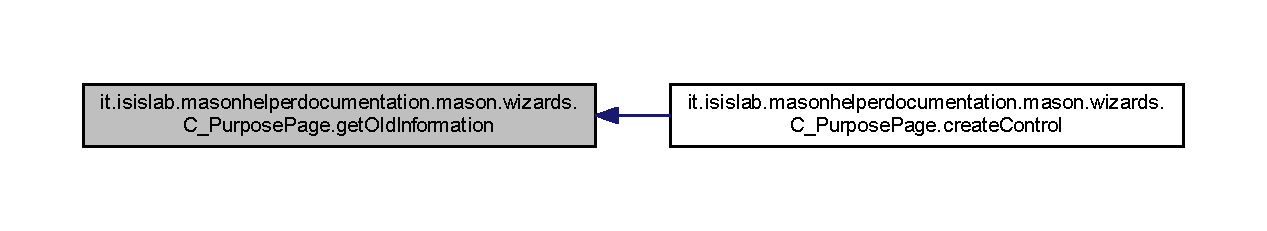
\includegraphics[width=350pt]{classit_1_1isislab_1_1masonhelperdocumentation_1_1mason_1_1wizards_1_1_c___purpose_page_acb3c2b59b784cc1d761a9d95b5300bb8_icgraph}
\end{center}
\end{figure}




\subsection{Member Data Documentation}
\hypertarget{classit_1_1isislab_1_1masonhelperdocumentation_1_1mason_1_1wizards_1_1_c___purpose_page_a1e19f349d9008f860de96a145f5ea5e7}{\index{it\-::isislab\-::masonhelperdocumentation\-::mason\-::wizards\-::\-C\-\_\-\-Purpose\-Page@{it\-::isislab\-::masonhelperdocumentation\-::mason\-::wizards\-::\-C\-\_\-\-Purpose\-Page}!page\-Description@{page\-Description}}
\index{page\-Description@{page\-Description}!it::isislab::masonhelperdocumentation::mason::wizards::C_PurposePage@{it\-::isislab\-::masonhelperdocumentation\-::mason\-::wizards\-::\-C\-\_\-\-Purpose\-Page}}
\subsubsection[{page\-Description}]{\setlength{\rightskip}{0pt plus 5cm}String it.\-isislab.\-masonhelperdocumentation.\-mason.\-wizards.\-C\-\_\-\-Purpose\-Page.\-page\-Description = \char`\"{}What is the purpose of the model?\char`\"{}\hspace{0.3cm}{\ttfamily [static]}, {\ttfamily [private]}}}\label{classit_1_1isislab_1_1masonhelperdocumentation_1_1mason_1_1wizards_1_1_c___purpose_page_a1e19f349d9008f860de96a145f5ea5e7}
\hypertarget{classit_1_1isislab_1_1masonhelperdocumentation_1_1mason_1_1wizards_1_1_c___purpose_page_a8441e960f1ba3f3315168635e8976822}{\index{it\-::isislab\-::masonhelperdocumentation\-::mason\-::wizards\-::\-C\-\_\-\-Purpose\-Page@{it\-::isislab\-::masonhelperdocumentation\-::mason\-::wizards\-::\-C\-\_\-\-Purpose\-Page}!sim\-State@{sim\-State}}
\index{sim\-State@{sim\-State}!it::isislab::masonhelperdocumentation::mason::wizards::C_PurposePage@{it\-::isislab\-::masonhelperdocumentation\-::mason\-::wizards\-::\-C\-\_\-\-Purpose\-Page}}
\subsubsection[{sim\-State}]{\setlength{\rightskip}{0pt plus 5cm}{\bf Sim\-State\-Analizer} it.\-isislab.\-masonhelperdocumentation.\-mason.\-wizards.\-C\-\_\-\-Purpose\-Page.\-sim\-State\hspace{0.3cm}{\ttfamily [private]}}}\label{classit_1_1isislab_1_1masonhelperdocumentation_1_1mason_1_1wizards_1_1_c___purpose_page_a8441e960f1ba3f3315168635e8976822}
\hypertarget{classit_1_1isislab_1_1masonhelperdocumentation_1_1mason_1_1wizards_1_1_c___purpose_page_abeec86a6fae75f2a485faeade141dd81}{\index{it\-::isislab\-::masonhelperdocumentation\-::mason\-::wizards\-::\-C\-\_\-\-Purpose\-Page@{it\-::isislab\-::masonhelperdocumentation\-::mason\-::wizards\-::\-C\-\_\-\-Purpose\-Page}!text@{text}}
\index{text@{text}!it::isislab::masonhelperdocumentation::mason::wizards::C_PurposePage@{it\-::isislab\-::masonhelperdocumentation\-::mason\-::wizards\-::\-C\-\_\-\-Purpose\-Page}}
\subsubsection[{text}]{\setlength{\rightskip}{0pt plus 5cm}Text it.\-isislab.\-masonhelperdocumentation.\-mason.\-wizards.\-C\-\_\-\-Purpose\-Page.\-text\hspace{0.3cm}{\ttfamily [private]}}}\label{classit_1_1isislab_1_1masonhelperdocumentation_1_1mason_1_1wizards_1_1_c___purpose_page_abeec86a6fae75f2a485faeade141dd81}


The documentation for this class was generated from the following file\-:\begin{DoxyCompactItemize}
\item 
src/it/isislab/masonhelperdocumentation/mason/wizards/\hyperlink{_c___purpose_page_8java}{C\-\_\-\-Purpose\-Page.\-java}\end{DoxyCompactItemize}

\hypertarget{classit_1_1isislab_1_1masonhelperdocumentation_1_1visitor_1_1_code_visitor}{\section{it.\-isislab.\-masonhelperdocumentation.\-visitor.\-Code\-Visitor Class Reference}
\label{classit_1_1isislab_1_1masonhelperdocumentation_1_1visitor_1_1_code_visitor}\index{it.\-isislab.\-masonhelperdocumentation.\-visitor.\-Code\-Visitor@{it.\-isislab.\-masonhelperdocumentation.\-visitor.\-Code\-Visitor}}
}


Inheritance diagram for it.\-isislab.\-masonhelperdocumentation.\-visitor.\-Code\-Visitor\-:
\nopagebreak
\begin{figure}[H]
\begin{center}
\leavevmode
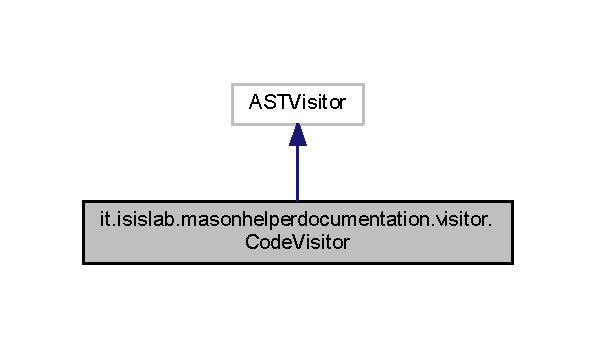
\includegraphics[width=286pt]{classit_1_1isislab_1_1masonhelperdocumentation_1_1visitor_1_1_code_visitor__inherit__graph}
\end{center}
\end{figure}


Collaboration diagram for it.\-isislab.\-masonhelperdocumentation.\-visitor.\-Code\-Visitor\-:
\nopagebreak
\begin{figure}[H]
\begin{center}
\leavevmode
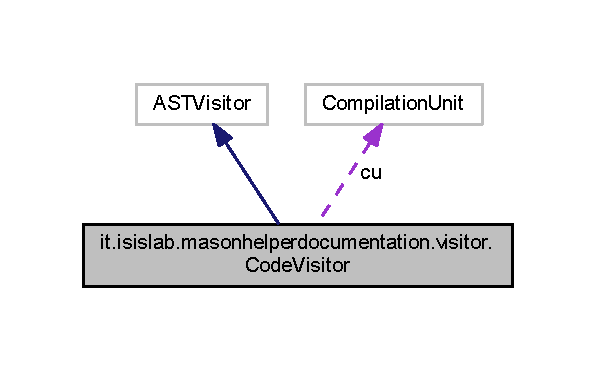
\includegraphics[width=286pt]{classit_1_1isislab_1_1masonhelperdocumentation_1_1visitor_1_1_code_visitor__coll__graph}
\end{center}
\end{figure}
\subsection*{Public Member Functions}
\begin{DoxyCompactItemize}
\item 
\hyperlink{classit_1_1isislab_1_1masonhelperdocumentation_1_1visitor_1_1_code_visitor_a187184161108b27007b877d0c2370443}{Code\-Visitor} (Compilation\-Unit \hyperlink{classit_1_1isislab_1_1masonhelperdocumentation_1_1visitor_1_1_code_visitor_af9088f73f92fd3640698ad4e660f042b}{cu})
\item 
boolean \hyperlink{classit_1_1isislab_1_1masonhelperdocumentation_1_1visitor_1_1_code_visitor_a8725175075e5b835707c806d7d168366}{visit} (If\-Statement node)
\item 
void \hyperlink{classit_1_1isislab_1_1masonhelperdocumentation_1_1visitor_1_1_code_visitor_ab5af98ceed9837f084b6d0a677b655ff}{end\-Visit} (If\-Statement node)
\item 
boolean \hyperlink{classit_1_1isislab_1_1masonhelperdocumentation_1_1visitor_1_1_code_visitor_ac93a6ee9bc2290dc054774d26a1e85f1}{visit} (For\-Statement f)
\item 
void \hyperlink{classit_1_1isislab_1_1masonhelperdocumentation_1_1visitor_1_1_code_visitor_ac0c818698da51575c8a9c9b6f643a96f}{end\-Visit} (For\-Statement node)
\item 
boolean \hyperlink{classit_1_1isislab_1_1masonhelperdocumentation_1_1visitor_1_1_code_visitor_afe7c0b57633a57e1cc2a5609163b48bd}{visit} (Do\-Statement d)
\item 
void \hyperlink{classit_1_1isislab_1_1masonhelperdocumentation_1_1visitor_1_1_code_visitor_aa83144733b831fd503c1cddb307abf68}{end\-Visit} (Do\-Statement node)
\item 
boolean \hyperlink{classit_1_1isislab_1_1masonhelperdocumentation_1_1visitor_1_1_code_visitor_a35fed6bc304be6fc1cf1b0d41e67cdea}{visit} (Switch\-Statement s)
\item 
void \hyperlink{classit_1_1isislab_1_1masonhelperdocumentation_1_1visitor_1_1_code_visitor_ac7190fc5f2c9e21dd1ffde65f3921d87}{end\-Visit} (Switch\-Statement node)
\item 
boolean \hyperlink{classit_1_1isislab_1_1masonhelperdocumentation_1_1visitor_1_1_code_visitor_a65b76f4e3876f0d044984dfe16c42d16}{visit} (Type\-Declaration t)
\item 
void \hyperlink{classit_1_1isislab_1_1masonhelperdocumentation_1_1visitor_1_1_code_visitor_ad08a404899ec7336cb57e02a6568ad09}{end\-Visit} (Type\-Declaration node)
\item 
boolean \hyperlink{classit_1_1isislab_1_1masonhelperdocumentation_1_1visitor_1_1_code_visitor_a2b41e9c8c3315dbb1fd18e6890a3842e}{visit} (Assignment node)
\item 
void \hyperlink{classit_1_1isislab_1_1masonhelperdocumentation_1_1visitor_1_1_code_visitor_a4efdef7b2bec3dad2b29f14c0bfe62d6}{end\-Visit} (Assignment node)
\item 
boolean \hyperlink{classit_1_1isislab_1_1masonhelperdocumentation_1_1visitor_1_1_code_visitor_a217f515da74b716c9d3fb43027be8301}{visit} (Method\-Invocation node)
\item 
void \hyperlink{classit_1_1isislab_1_1masonhelperdocumentation_1_1visitor_1_1_code_visitor_a0621bb29c4a918f034a2d7a8815cba6d}{end\-Visit} (Method\-Invocation node)
\item 
String \hyperlink{classit_1_1isislab_1_1masonhelperdocumentation_1_1visitor_1_1_code_visitor_a464d8e1b4691e88a39a287c1543cbdd2}{get\-Information\-\_\-s} ()
\end{DoxyCompactItemize}
\subsection*{Private Attributes}
\begin{DoxyCompactItemize}
\item 
Compilation\-Unit \hyperlink{classit_1_1isislab_1_1masonhelperdocumentation_1_1visitor_1_1_code_visitor_af9088f73f92fd3640698ad4e660f042b}{cu}
\item 
String \hyperlink{classit_1_1isislab_1_1masonhelperdocumentation_1_1visitor_1_1_code_visitor_a8bfc263e47218ff87b62a5ad9b1294e7}{information\-\_\-s}
\end{DoxyCompactItemize}


\subsection{Detailed Description}
This class represent a visitor for method. Purpose of this class is extract a description of method in natural language. \begin{DoxyAuthor}{Author}
Romano Simone 0512101343 
\end{DoxyAuthor}


\subsection{Constructor \& Destructor Documentation}
\hypertarget{classit_1_1isislab_1_1masonhelperdocumentation_1_1visitor_1_1_code_visitor_a187184161108b27007b877d0c2370443}{\index{it\-::isislab\-::masonhelperdocumentation\-::visitor\-::\-Code\-Visitor@{it\-::isislab\-::masonhelperdocumentation\-::visitor\-::\-Code\-Visitor}!Code\-Visitor@{Code\-Visitor}}
\index{Code\-Visitor@{Code\-Visitor}!it::isislab::masonhelperdocumentation::visitor::CodeVisitor@{it\-::isislab\-::masonhelperdocumentation\-::visitor\-::\-Code\-Visitor}}
\subsubsection[{Code\-Visitor}]{\setlength{\rightskip}{0pt plus 5cm}it.\-isislab.\-masonhelperdocumentation.\-visitor.\-Code\-Visitor.\-Code\-Visitor (
\begin{DoxyParamCaption}
\item[{Compilation\-Unit}]{cu}
\end{DoxyParamCaption}
)}}\label{classit_1_1isislab_1_1masonhelperdocumentation_1_1visitor_1_1_code_visitor_a187184161108b27007b877d0c2370443}

\begin{DoxyCode}
34                                           \{
35         this.cu = \hyperlink{classit_1_1isislab_1_1masonhelperdocumentation_1_1visitor_1_1_code_visitor_af9088f73f92fd3640698ad4e660f042b}{cu};
36         \hyperlink{classit_1_1isislab_1_1masonhelperdocumentation_1_1visitor_1_1_code_visitor_a8bfc263e47218ff87b62a5ad9b1294e7}{information\_s} = \textcolor{stringliteral}{""};
37     \}
\end{DoxyCode}


Here is the caller graph for this function\-:
\nopagebreak
\begin{figure}[H]
\begin{center}
\leavevmode
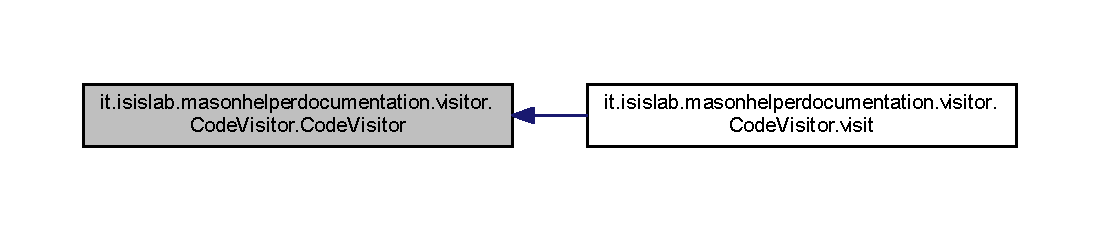
\includegraphics[width=350pt]{classit_1_1isislab_1_1masonhelperdocumentation_1_1visitor_1_1_code_visitor_a187184161108b27007b877d0c2370443_icgraph}
\end{center}
\end{figure}




\subsection{Member Function Documentation}
\hypertarget{classit_1_1isislab_1_1masonhelperdocumentation_1_1visitor_1_1_code_visitor_ab5af98ceed9837f084b6d0a677b655ff}{\index{it\-::isislab\-::masonhelperdocumentation\-::visitor\-::\-Code\-Visitor@{it\-::isislab\-::masonhelperdocumentation\-::visitor\-::\-Code\-Visitor}!end\-Visit@{end\-Visit}}
\index{end\-Visit@{end\-Visit}!it::isislab::masonhelperdocumentation::visitor::CodeVisitor@{it\-::isislab\-::masonhelperdocumentation\-::visitor\-::\-Code\-Visitor}}
\subsubsection[{end\-Visit}]{\setlength{\rightskip}{0pt plus 5cm}void it.\-isislab.\-masonhelperdocumentation.\-visitor.\-Code\-Visitor.\-end\-Visit (
\begin{DoxyParamCaption}
\item[{If\-Statement}]{node}
\end{DoxyParamCaption}
)}}\label{classit_1_1isislab_1_1masonhelperdocumentation_1_1visitor_1_1_code_visitor_ab5af98ceed9837f084b6d0a677b655ff}

\begin{DoxyCode}
45                                           \{
46         \hyperlink{classit_1_1isislab_1_1masonhelperdocumentation_1_1visitor_1_1_code_visitor_a8bfc263e47218ff87b62a5ad9b1294e7}{information\_s} += \hyperlink{classit_1_1isislab_1_1masonhelperdocumentation_1_1visitor_1_1_messages_ac30d6eb5c0dfe157ff4707375c9bc967}{Messages.Visitor\_EndIf};
47     \}
\end{DoxyCode}
\hypertarget{classit_1_1isislab_1_1masonhelperdocumentation_1_1visitor_1_1_code_visitor_ac0c818698da51575c8a9c9b6f643a96f}{\index{it\-::isislab\-::masonhelperdocumentation\-::visitor\-::\-Code\-Visitor@{it\-::isislab\-::masonhelperdocumentation\-::visitor\-::\-Code\-Visitor}!end\-Visit@{end\-Visit}}
\index{end\-Visit@{end\-Visit}!it::isislab::masonhelperdocumentation::visitor::CodeVisitor@{it\-::isislab\-::masonhelperdocumentation\-::visitor\-::\-Code\-Visitor}}
\subsubsection[{end\-Visit}]{\setlength{\rightskip}{0pt plus 5cm}void it.\-isislab.\-masonhelperdocumentation.\-visitor.\-Code\-Visitor.\-end\-Visit (
\begin{DoxyParamCaption}
\item[{For\-Statement}]{node}
\end{DoxyParamCaption}
)}}\label{classit_1_1isislab_1_1masonhelperdocumentation_1_1visitor_1_1_code_visitor_ac0c818698da51575c8a9c9b6f643a96f}

\begin{DoxyCode}
54                                            \{
55         \hyperlink{classit_1_1isislab_1_1masonhelperdocumentation_1_1visitor_1_1_code_visitor_a8bfc263e47218ff87b62a5ad9b1294e7}{information\_s} += \hyperlink{classit_1_1isislab_1_1masonhelperdocumentation_1_1visitor_1_1_messages_a22bdeb4184a47b5dca73a5f6be80829f}{Messages.Visitor\_EndFor}; \textcolor{comment}{//$NON-NLS-2$;}
56     \}
\end{DoxyCode}
\hypertarget{classit_1_1isislab_1_1masonhelperdocumentation_1_1visitor_1_1_code_visitor_aa83144733b831fd503c1cddb307abf68}{\index{it\-::isislab\-::masonhelperdocumentation\-::visitor\-::\-Code\-Visitor@{it\-::isislab\-::masonhelperdocumentation\-::visitor\-::\-Code\-Visitor}!end\-Visit@{end\-Visit}}
\index{end\-Visit@{end\-Visit}!it::isislab::masonhelperdocumentation::visitor::CodeVisitor@{it\-::isislab\-::masonhelperdocumentation\-::visitor\-::\-Code\-Visitor}}
\subsubsection[{end\-Visit}]{\setlength{\rightskip}{0pt plus 5cm}void it.\-isislab.\-masonhelperdocumentation.\-visitor.\-Code\-Visitor.\-end\-Visit (
\begin{DoxyParamCaption}
\item[{Do\-Statement}]{node}
\end{DoxyParamCaption}
)}}\label{classit_1_1isislab_1_1masonhelperdocumentation_1_1visitor_1_1_code_visitor_aa83144733b831fd503c1cddb307abf68}

\begin{DoxyCode}
63                                           \{
64         \hyperlink{classit_1_1isislab_1_1masonhelperdocumentation_1_1visitor_1_1_code_visitor_a8bfc263e47218ff87b62a5ad9b1294e7}{information\_s} += \hyperlink{classit_1_1isislab_1_1masonhelperdocumentation_1_1visitor_1_1_messages_a51a130626b490a71efd339a23c0e4ddf}{Messages.Visitor\_DoWhileEnd};
65     \}
\end{DoxyCode}
\hypertarget{classit_1_1isislab_1_1masonhelperdocumentation_1_1visitor_1_1_code_visitor_ac7190fc5f2c9e21dd1ffde65f3921d87}{\index{it\-::isislab\-::masonhelperdocumentation\-::visitor\-::\-Code\-Visitor@{it\-::isislab\-::masonhelperdocumentation\-::visitor\-::\-Code\-Visitor}!end\-Visit@{end\-Visit}}
\index{end\-Visit@{end\-Visit}!it::isislab::masonhelperdocumentation::visitor::CodeVisitor@{it\-::isislab\-::masonhelperdocumentation\-::visitor\-::\-Code\-Visitor}}
\subsubsection[{end\-Visit}]{\setlength{\rightskip}{0pt plus 5cm}void it.\-isislab.\-masonhelperdocumentation.\-visitor.\-Code\-Visitor.\-end\-Visit (
\begin{DoxyParamCaption}
\item[{Switch\-Statement}]{node}
\end{DoxyParamCaption}
)}}\label{classit_1_1isislab_1_1masonhelperdocumentation_1_1visitor_1_1_code_visitor_ac7190fc5f2c9e21dd1ffde65f3921d87}

\begin{DoxyCode}
72                                               \{
73         \hyperlink{classit_1_1isislab_1_1masonhelperdocumentation_1_1visitor_1_1_code_visitor_a8bfc263e47218ff87b62a5ad9b1294e7}{information\_s} += \hyperlink{classit_1_1isislab_1_1masonhelperdocumentation_1_1visitor_1_1_messages_ad36ac06cbc96b50d396a7400b4faf972}{Messages.Visitor\_EndSwitch};
74     \}
\end{DoxyCode}
\hypertarget{classit_1_1isislab_1_1masonhelperdocumentation_1_1visitor_1_1_code_visitor_ad08a404899ec7336cb57e02a6568ad09}{\index{it\-::isislab\-::masonhelperdocumentation\-::visitor\-::\-Code\-Visitor@{it\-::isislab\-::masonhelperdocumentation\-::visitor\-::\-Code\-Visitor}!end\-Visit@{end\-Visit}}
\index{end\-Visit@{end\-Visit}!it::isislab::masonhelperdocumentation::visitor::CodeVisitor@{it\-::isislab\-::masonhelperdocumentation\-::visitor\-::\-Code\-Visitor}}
\subsubsection[{end\-Visit}]{\setlength{\rightskip}{0pt plus 5cm}void it.\-isislab.\-masonhelperdocumentation.\-visitor.\-Code\-Visitor.\-end\-Visit (
\begin{DoxyParamCaption}
\item[{Type\-Declaration}]{node}
\end{DoxyParamCaption}
)}}\label{classit_1_1isislab_1_1masonhelperdocumentation_1_1visitor_1_1_code_visitor_ad08a404899ec7336cb57e02a6568ad09}

\begin{DoxyCode}
81                                               \{
82         \hyperlink{classit_1_1isislab_1_1masonhelperdocumentation_1_1visitor_1_1_code_visitor_a8bfc263e47218ff87b62a5ad9b1294e7}{information\_s} += \hyperlink{classit_1_1isislab_1_1masonhelperdocumentation_1_1visitor_1_1_messages_aea00da7022007d6739ca682635b64092}{Messages.Visitor\_EndTypeDeclaration}
      ;
83     \}
\end{DoxyCode}
\hypertarget{classit_1_1isislab_1_1masonhelperdocumentation_1_1visitor_1_1_code_visitor_a4efdef7b2bec3dad2b29f14c0bfe62d6}{\index{it\-::isislab\-::masonhelperdocumentation\-::visitor\-::\-Code\-Visitor@{it\-::isislab\-::masonhelperdocumentation\-::visitor\-::\-Code\-Visitor}!end\-Visit@{end\-Visit}}
\index{end\-Visit@{end\-Visit}!it::isislab::masonhelperdocumentation::visitor::CodeVisitor@{it\-::isislab\-::masonhelperdocumentation\-::visitor\-::\-Code\-Visitor}}
\subsubsection[{end\-Visit}]{\setlength{\rightskip}{0pt plus 5cm}void it.\-isislab.\-masonhelperdocumentation.\-visitor.\-Code\-Visitor.\-end\-Visit (
\begin{DoxyParamCaption}
\item[{Assignment}]{node}
\end{DoxyParamCaption}
)}}\label{classit_1_1isislab_1_1masonhelperdocumentation_1_1visitor_1_1_code_visitor_a4efdef7b2bec3dad2b29f14c0bfe62d6}

\begin{DoxyCode}
90                                          \{
91         \hyperlink{classit_1_1isislab_1_1masonhelperdocumentation_1_1visitor_1_1_code_visitor_a8bfc263e47218ff87b62a5ad9b1294e7}{information\_s} += \hyperlink{classit_1_1isislab_1_1masonhelperdocumentation_1_1visitor_1_1_messages_ad3b39e81af7e7f2d36f3b9522b0d7ea5}{Messages.Visitor\_EndAssignent};
92     \}
\end{DoxyCode}
\hypertarget{classit_1_1isislab_1_1masonhelperdocumentation_1_1visitor_1_1_code_visitor_a0621bb29c4a918f034a2d7a8815cba6d}{\index{it\-::isislab\-::masonhelperdocumentation\-::visitor\-::\-Code\-Visitor@{it\-::isislab\-::masonhelperdocumentation\-::visitor\-::\-Code\-Visitor}!end\-Visit@{end\-Visit}}
\index{end\-Visit@{end\-Visit}!it::isislab::masonhelperdocumentation::visitor::CodeVisitor@{it\-::isislab\-::masonhelperdocumentation\-::visitor\-::\-Code\-Visitor}}
\subsubsection[{end\-Visit}]{\setlength{\rightskip}{0pt plus 5cm}void it.\-isislab.\-masonhelperdocumentation.\-visitor.\-Code\-Visitor.\-end\-Visit (
\begin{DoxyParamCaption}
\item[{Method\-Invocation}]{node}
\end{DoxyParamCaption}
)}}\label{classit_1_1isislab_1_1masonhelperdocumentation_1_1visitor_1_1_code_visitor_a0621bb29c4a918f034a2d7a8815cba6d}

\begin{DoxyCode}
109                                                \{
110         \hyperlink{classit_1_1isislab_1_1masonhelperdocumentation_1_1visitor_1_1_code_visitor_a8bfc263e47218ff87b62a5ad9b1294e7}{information\_s} += Messages.Visitor\_EndInvocation + node.getName() + Messages.
      Visitor\_EndInvocation1;
111     \}
\end{DoxyCode}
\hypertarget{classit_1_1isislab_1_1masonhelperdocumentation_1_1visitor_1_1_code_visitor_a464d8e1b4691e88a39a287c1543cbdd2}{\index{it\-::isislab\-::masonhelperdocumentation\-::visitor\-::\-Code\-Visitor@{it\-::isislab\-::masonhelperdocumentation\-::visitor\-::\-Code\-Visitor}!get\-Information\-\_\-s@{get\-Information\-\_\-s}}
\index{get\-Information\-\_\-s@{get\-Information\-\_\-s}!it::isislab::masonhelperdocumentation::visitor::CodeVisitor@{it\-::isislab\-::masonhelperdocumentation\-::visitor\-::\-Code\-Visitor}}
\subsubsection[{get\-Information\-\_\-s}]{\setlength{\rightskip}{0pt plus 5cm}String it.\-isislab.\-masonhelperdocumentation.\-visitor.\-Code\-Visitor.\-get\-Information\-\_\-s (
\begin{DoxyParamCaption}
{}
\end{DoxyParamCaption}
)}}\label{classit_1_1isislab_1_1masonhelperdocumentation_1_1visitor_1_1_code_visitor_a464d8e1b4691e88a39a287c1543cbdd2}

\begin{DoxyCode}
113                                      \{
114         \textcolor{keywordflow}{return} \hyperlink{classit_1_1isislab_1_1masonhelperdocumentation_1_1visitor_1_1_code_visitor_a8bfc263e47218ff87b62a5ad9b1294e7}{information\_s} + \hyperlink{classit_1_1isislab_1_1masonhelperdocumentation_1_1visitor_1_1_messages_aecf94c4bd9def64267445d4624298066}{Messages.Visitor\_EndMethod};
115     \}
\end{DoxyCode}
\hypertarget{classit_1_1isislab_1_1masonhelperdocumentation_1_1visitor_1_1_code_visitor_a8725175075e5b835707c806d7d168366}{\index{it\-::isislab\-::masonhelperdocumentation\-::visitor\-::\-Code\-Visitor@{it\-::isislab\-::masonhelperdocumentation\-::visitor\-::\-Code\-Visitor}!visit@{visit}}
\index{visit@{visit}!it::isislab::masonhelperdocumentation::visitor::CodeVisitor@{it\-::isislab\-::masonhelperdocumentation\-::visitor\-::\-Code\-Visitor}}
\subsubsection[{visit}]{\setlength{\rightskip}{0pt plus 5cm}boolean it.\-isislab.\-masonhelperdocumentation.\-visitor.\-Code\-Visitor.\-visit (
\begin{DoxyParamCaption}
\item[{If\-Statement}]{node}
\end{DoxyParamCaption}
)}}\label{classit_1_1isislab_1_1masonhelperdocumentation_1_1visitor_1_1_code_visitor_a8725175075e5b835707c806d7d168366}

\begin{DoxyCode}
40                                            \{
41         \hyperlink{classit_1_1isislab_1_1masonhelperdocumentation_1_1visitor_1_1_code_visitor_a8bfc263e47218ff87b62a5ad9b1294e7}{information\_s} += Messages.Visitor\_If1 + node.getExpression() + \textcolor{stringliteral}{" "}; \textcolor{comment}{//$NON-NLS-2$}
42         \textcolor{keywordflow}{return} super.visit(node);
43     \}
\end{DoxyCode}
\hypertarget{classit_1_1isislab_1_1masonhelperdocumentation_1_1visitor_1_1_code_visitor_ac93a6ee9bc2290dc054774d26a1e85f1}{\index{it\-::isislab\-::masonhelperdocumentation\-::visitor\-::\-Code\-Visitor@{it\-::isislab\-::masonhelperdocumentation\-::visitor\-::\-Code\-Visitor}!visit@{visit}}
\index{visit@{visit}!it::isislab::masonhelperdocumentation::visitor::CodeVisitor@{it\-::isislab\-::masonhelperdocumentation\-::visitor\-::\-Code\-Visitor}}
\subsubsection[{visit}]{\setlength{\rightskip}{0pt plus 5cm}boolean it.\-isislab.\-masonhelperdocumentation.\-visitor.\-Code\-Visitor.\-visit (
\begin{DoxyParamCaption}
\item[{For\-Statement}]{f}
\end{DoxyParamCaption}
)}}\label{classit_1_1isislab_1_1masonhelperdocumentation_1_1visitor_1_1_code_visitor_ac93a6ee9bc2290dc054774d26a1e85f1}

\begin{DoxyCode}
49                                         \{
50         \hyperlink{classit_1_1isislab_1_1masonhelperdocumentation_1_1visitor_1_1_code_visitor_a8bfc263e47218ff87b62a5ad9b1294e7}{information\_s} += Messages.Visitor\_While1 + f.getExpression() + \textcolor{stringliteral}{" "}; \textcolor{comment}{//$NON-NLS-2$}
51         \textcolor{keywordflow}{return} super.visit(f);
52     \}
\end{DoxyCode}
\hypertarget{classit_1_1isislab_1_1masonhelperdocumentation_1_1visitor_1_1_code_visitor_afe7c0b57633a57e1cc2a5609163b48bd}{\index{it\-::isislab\-::masonhelperdocumentation\-::visitor\-::\-Code\-Visitor@{it\-::isislab\-::masonhelperdocumentation\-::visitor\-::\-Code\-Visitor}!visit@{visit}}
\index{visit@{visit}!it::isislab::masonhelperdocumentation::visitor::CodeVisitor@{it\-::isislab\-::masonhelperdocumentation\-::visitor\-::\-Code\-Visitor}}
\subsubsection[{visit}]{\setlength{\rightskip}{0pt plus 5cm}boolean it.\-isislab.\-masonhelperdocumentation.\-visitor.\-Code\-Visitor.\-visit (
\begin{DoxyParamCaption}
\item[{Do\-Statement}]{d}
\end{DoxyParamCaption}
)}}\label{classit_1_1isislab_1_1masonhelperdocumentation_1_1visitor_1_1_code_visitor_afe7c0b57633a57e1cc2a5609163b48bd}

\begin{DoxyCode}
58                                         \{
59         \hyperlink{classit_1_1isislab_1_1masonhelperdocumentation_1_1visitor_1_1_code_visitor_a8bfc263e47218ff87b62a5ad9b1294e7}{information\_s} += Messages.Visitor\_Do1 + d.getExpression() + \textcolor{stringliteral}{" "}; \textcolor{comment}{//$NON-NLS-2$}
60         \textcolor{keywordflow}{return} super.visit(d);
61     \}
\end{DoxyCode}
\hypertarget{classit_1_1isislab_1_1masonhelperdocumentation_1_1visitor_1_1_code_visitor_a35fed6bc304be6fc1cf1b0d41e67cdea}{\index{it\-::isislab\-::masonhelperdocumentation\-::visitor\-::\-Code\-Visitor@{it\-::isislab\-::masonhelperdocumentation\-::visitor\-::\-Code\-Visitor}!visit@{visit}}
\index{visit@{visit}!it::isislab::masonhelperdocumentation::visitor::CodeVisitor@{it\-::isislab\-::masonhelperdocumentation\-::visitor\-::\-Code\-Visitor}}
\subsubsection[{visit}]{\setlength{\rightskip}{0pt plus 5cm}boolean it.\-isislab.\-masonhelperdocumentation.\-visitor.\-Code\-Visitor.\-visit (
\begin{DoxyParamCaption}
\item[{Switch\-Statement}]{s}
\end{DoxyParamCaption}
)}}\label{classit_1_1isislab_1_1masonhelperdocumentation_1_1visitor_1_1_code_visitor_a35fed6bc304be6fc1cf1b0d41e67cdea}

\begin{DoxyCode}
67                                            \{
68         \hyperlink{classit_1_1isislab_1_1masonhelperdocumentation_1_1visitor_1_1_code_visitor_a8bfc263e47218ff87b62a5ad9b1294e7}{information\_s} += Messages.Visitor\_SwitchInfo + s.getExpression() + \textcolor{stringliteral}{" "}; \textcolor{comment}{//$NON-NLS-2$}
69         \textcolor{keywordflow}{return} super.visit(s);
70     \}
\end{DoxyCode}
\hypertarget{classit_1_1isislab_1_1masonhelperdocumentation_1_1visitor_1_1_code_visitor_a65b76f4e3876f0d044984dfe16c42d16}{\index{it\-::isislab\-::masonhelperdocumentation\-::visitor\-::\-Code\-Visitor@{it\-::isislab\-::masonhelperdocumentation\-::visitor\-::\-Code\-Visitor}!visit@{visit}}
\index{visit@{visit}!it::isislab::masonhelperdocumentation::visitor::CodeVisitor@{it\-::isislab\-::masonhelperdocumentation\-::visitor\-::\-Code\-Visitor}}
\subsubsection[{visit}]{\setlength{\rightskip}{0pt plus 5cm}boolean it.\-isislab.\-masonhelperdocumentation.\-visitor.\-Code\-Visitor.\-visit (
\begin{DoxyParamCaption}
\item[{Type\-Declaration}]{t}
\end{DoxyParamCaption}
)}}\label{classit_1_1isislab_1_1masonhelperdocumentation_1_1visitor_1_1_code_visitor_a65b76f4e3876f0d044984dfe16c42d16}

\begin{DoxyCode}
76                                            \{
77         \hyperlink{classit_1_1isislab_1_1masonhelperdocumentation_1_1visitor_1_1_code_visitor_a8bfc263e47218ff87b62a5ad9b1294e7}{information\_s} += Messages.Visitor\_TypeDeclaration + t.getName();
78         \textcolor{keywordflow}{return} super.visit(t);
79     \}
\end{DoxyCode}
\hypertarget{classit_1_1isislab_1_1masonhelperdocumentation_1_1visitor_1_1_code_visitor_a2b41e9c8c3315dbb1fd18e6890a3842e}{\index{it\-::isislab\-::masonhelperdocumentation\-::visitor\-::\-Code\-Visitor@{it\-::isislab\-::masonhelperdocumentation\-::visitor\-::\-Code\-Visitor}!visit@{visit}}
\index{visit@{visit}!it::isislab::masonhelperdocumentation::visitor::CodeVisitor@{it\-::isislab\-::masonhelperdocumentation\-::visitor\-::\-Code\-Visitor}}
\subsubsection[{visit}]{\setlength{\rightskip}{0pt plus 5cm}boolean it.\-isislab.\-masonhelperdocumentation.\-visitor.\-Code\-Visitor.\-visit (
\begin{DoxyParamCaption}
\item[{Assignment}]{node}
\end{DoxyParamCaption}
)}}\label{classit_1_1isislab_1_1masonhelperdocumentation_1_1visitor_1_1_code_visitor_a2b41e9c8c3315dbb1fd18e6890a3842e}

\begin{DoxyCode}
85                                          \{
86         \hyperlink{classit_1_1isislab_1_1masonhelperdocumentation_1_1visitor_1_1_code_visitor_a8bfc263e47218ff87b62a5ad9b1294e7}{information\_s} += Messages.Visitor\_Assignment + node.getLeftHandSide() + Messages.
      Visitor\_Assignemnt1 + node.getRightHandSide() + \textcolor{stringliteral}{" "}; \textcolor{comment}{//$NON-NLS-3$}
87         \textcolor{keywordflow}{return} super.visit(node);
88     \}
\end{DoxyCode}
\hypertarget{classit_1_1isislab_1_1masonhelperdocumentation_1_1visitor_1_1_code_visitor_a217f515da74b716c9d3fb43027be8301}{\index{it\-::isislab\-::masonhelperdocumentation\-::visitor\-::\-Code\-Visitor@{it\-::isislab\-::masonhelperdocumentation\-::visitor\-::\-Code\-Visitor}!visit@{visit}}
\index{visit@{visit}!it::isislab::masonhelperdocumentation::visitor::CodeVisitor@{it\-::isislab\-::masonhelperdocumentation\-::visitor\-::\-Code\-Visitor}}
\subsubsection[{visit}]{\setlength{\rightskip}{0pt plus 5cm}boolean it.\-isislab.\-masonhelperdocumentation.\-visitor.\-Code\-Visitor.\-visit (
\begin{DoxyParamCaption}
\item[{Method\-Invocation}]{node}
\end{DoxyParamCaption}
)}}\label{classit_1_1isislab_1_1masonhelperdocumentation_1_1visitor_1_1_code_visitor_a217f515da74b716c9d3fb43027be8301}

\begin{DoxyCode}
94                                                 \{
95         \textcolor{keywordtype}{boolean} visitedSubmetod = \textcolor{keyword}{false};
96         \hyperlink{classit_1_1isislab_1_1masonhelperdocumentation_1_1visitor_1_1_code_visitor_a8bfc263e47218ff87b62a5ad9b1294e7}{information\_s} += \textcolor{stringliteral}{"Invoke method "} + node.getName();
97         ArrayList<Method> method\_s = GlobalUtility.getAllMethods(\hyperlink{classit_1_1isislab_1_1masonhelperdocumentation_1_1visitor_1_1_code_visitor_af9088f73f92fd3640698ad4e660f042b}{cu});
98         \textcolor{keywordflow}{for} (Method m : method\_s)\{
99             \textcolor{keywordflow}{if} (m.getName().toString().equals(node.getName().toString()))\{
100                 visitedSubmetod = \textcolor{keyword}{true};
101                 \hyperlink{classit_1_1isislab_1_1masonhelperdocumentation_1_1visitor_1_1_code_visitor_a8bfc263e47218ff87b62a5ad9b1294e7}{information\_s} += \textcolor{stringliteral}{" that: "};
102                 m.getMethod().getBody().accept(\textcolor{keyword}{new} \hyperlink{classit_1_1isislab_1_1masonhelperdocumentation_1_1visitor_1_1_code_visitor_a187184161108b27007b877d0c2370443}{CodeVisitor}(\hyperlink{classit_1_1isislab_1_1masonhelperdocumentation_1_1visitor_1_1_code_visitor_af9088f73f92fd3640698ad4e660f042b}{cu}));
103             \}
104         \}
105         \textcolor{keywordflow}{if} (!visitedSubmetod) \hyperlink{classit_1_1isislab_1_1masonhelperdocumentation_1_1visitor_1_1_code_visitor_a8bfc263e47218ff87b62a5ad9b1294e7}{information\_s} += \textcolor{stringliteral}{".\(\backslash\)n"};
106         \textcolor{keywordflow}{return} super.visit(node);
107     \}
\end{DoxyCode}


Here is the call graph for this function\-:
\nopagebreak
\begin{figure}[H]
\begin{center}
\leavevmode
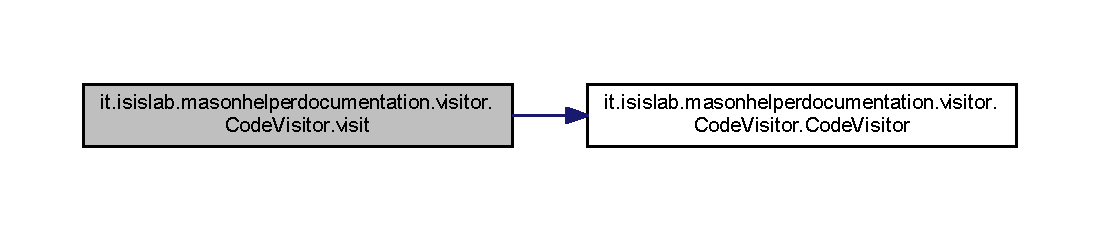
\includegraphics[width=350pt]{classit_1_1isislab_1_1masonhelperdocumentation_1_1visitor_1_1_code_visitor_a217f515da74b716c9d3fb43027be8301_cgraph}
\end{center}
\end{figure}




\subsection{Member Data Documentation}
\hypertarget{classit_1_1isislab_1_1masonhelperdocumentation_1_1visitor_1_1_code_visitor_af9088f73f92fd3640698ad4e660f042b}{\index{it\-::isislab\-::masonhelperdocumentation\-::visitor\-::\-Code\-Visitor@{it\-::isislab\-::masonhelperdocumentation\-::visitor\-::\-Code\-Visitor}!cu@{cu}}
\index{cu@{cu}!it::isislab::masonhelperdocumentation::visitor::CodeVisitor@{it\-::isislab\-::masonhelperdocumentation\-::visitor\-::\-Code\-Visitor}}
\subsubsection[{cu}]{\setlength{\rightskip}{0pt plus 5cm}Compilation\-Unit it.\-isislab.\-masonhelperdocumentation.\-visitor.\-Code\-Visitor.\-cu\hspace{0.3cm}{\ttfamily [private]}}}\label{classit_1_1isislab_1_1masonhelperdocumentation_1_1visitor_1_1_code_visitor_af9088f73f92fd3640698ad4e660f042b}
\hypertarget{classit_1_1isislab_1_1masonhelperdocumentation_1_1visitor_1_1_code_visitor_a8bfc263e47218ff87b62a5ad9b1294e7}{\index{it\-::isislab\-::masonhelperdocumentation\-::visitor\-::\-Code\-Visitor@{it\-::isislab\-::masonhelperdocumentation\-::visitor\-::\-Code\-Visitor}!information\-\_\-s@{information\-\_\-s}}
\index{information\-\_\-s@{information\-\_\-s}!it::isislab::masonhelperdocumentation::visitor::CodeVisitor@{it\-::isislab\-::masonhelperdocumentation\-::visitor\-::\-Code\-Visitor}}
\subsubsection[{information\-\_\-s}]{\setlength{\rightskip}{0pt plus 5cm}String it.\-isislab.\-masonhelperdocumentation.\-visitor.\-Code\-Visitor.\-information\-\_\-s\hspace{0.3cm}{\ttfamily [private]}}}\label{classit_1_1isislab_1_1masonhelperdocumentation_1_1visitor_1_1_code_visitor_a8bfc263e47218ff87b62a5ad9b1294e7}


The documentation for this class was generated from the following file\-:\begin{DoxyCompactItemize}
\item 
git/masonhelperdocumentation/src/it/isislab/masonhelperdocumentation/visitor/\hyperlink{_code_visitor_8java}{Code\-Visitor.\-java}\end{DoxyCompactItemize}

\hypertarget{classit_1_1isislab_1_1masonhelperdocumentation_1_1mason_1_1control_1_1_config_file}{\section{it.\-isislab.\-masonhelperdocumentation.\-mason.\-control.\-Config\-File Class Reference}
\label{classit_1_1isislab_1_1masonhelperdocumentation_1_1mason_1_1control_1_1_config_file}\index{it.\-isislab.\-masonhelperdocumentation.\-mason.\-control.\-Config\-File@{it.\-isislab.\-masonhelperdocumentation.\-mason.\-control.\-Config\-File}}
}


Collaboration diagram for it.\-isislab.\-masonhelperdocumentation.\-mason.\-control.\-Config\-File\-:
\nopagebreak
\begin{figure}[H]
\begin{center}
\leavevmode
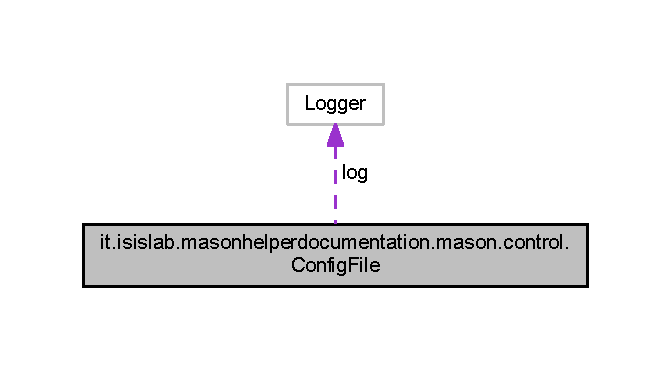
\includegraphics[width=322pt]{classit_1_1isislab_1_1masonhelperdocumentation_1_1mason_1_1control_1_1_config_file__coll__graph}
\end{center}
\end{figure}
\subsection*{Static Public Member Functions}
\begin{DoxyCompactItemize}
\item 
static String \hyperlink{classit_1_1isislab_1_1masonhelperdocumentation_1_1mason_1_1control_1_1_config_file_afc023838475034a60185402e9cedbfba}{get\-Dir} ()
\item 
static void \hyperlink{classit_1_1isislab_1_1masonhelperdocumentation_1_1mason_1_1control_1_1_config_file_a29d4bd9c148d1d7576cef7bcaf796172}{set\-Property} (String key, String value)
\item 
static String \hyperlink{classit_1_1isislab_1_1masonhelperdocumentation_1_1mason_1_1control_1_1_config_file_a7bcf08b34e48f0c5116d796d616113f0}{get\-Value} (String key)
\item 
static String \hyperlink{classit_1_1isislab_1_1masonhelperdocumentation_1_1mason_1_1control_1_1_config_file_a066e1a4a3eb3969e1d59776ba39caac1}{gett\-O\-D\-D\-Path} ()
\end{DoxyCompactItemize}
\subsection*{Static Private Member Functions}
\begin{DoxyCompactItemize}
\item 
static File \hyperlink{classit_1_1isislab_1_1masonhelperdocumentation_1_1mason_1_1control_1_1_config_file_ac533dd01e862be359ae060d278daf1ea}{get\-Config\-File} ()
\end{DoxyCompactItemize}
\subsection*{Static Private Attributes}
\begin{DoxyCompactItemize}
\item 
static Logger \hyperlink{classit_1_1isislab_1_1masonhelperdocumentation_1_1mason_1_1control_1_1_config_file_a1e0cc7c39d846dcf3dd9def42f836e89}{log} = Logger.\-get\-Logger(\char`\"{}global\char`\"{})
\item 
static String \hyperlink{classit_1_1isislab_1_1masonhelperdocumentation_1_1mason_1_1control_1_1_config_file_a7d8bbffdbfca146a398ed0bba454f347}{dir\-Name} = \char`\"{}M\-A\-S\-O\-N\-Helper\-Documentation\-\_\-\char`\"{}
\item 
static String \hyperlink{classit_1_1isislab_1_1masonhelperdocumentation_1_1mason_1_1control_1_1_config_file_a46a4e9d3359f002ff462e19976987878}{config\-File\-Name} = \char`\"{}config\-M\-A\-S\-O\-N\-Helper.\-dat\char`\"{}
\end{DoxyCompactItemize}


\subsection{Detailed Description}
This class manages config file.

\begin{DoxyAuthor}{Author}
Romano Simone 0512101343 
\end{DoxyAuthor}


\subsection{Member Function Documentation}
\hypertarget{classit_1_1isislab_1_1masonhelperdocumentation_1_1mason_1_1control_1_1_config_file_ac533dd01e862be359ae060d278daf1ea}{\index{it\-::isislab\-::masonhelperdocumentation\-::mason\-::control\-::\-Config\-File@{it\-::isislab\-::masonhelperdocumentation\-::mason\-::control\-::\-Config\-File}!get\-Config\-File@{get\-Config\-File}}
\index{get\-Config\-File@{get\-Config\-File}!it::isislab::masonhelperdocumentation::mason::control::ConfigFile@{it\-::isislab\-::masonhelperdocumentation\-::mason\-::control\-::\-Config\-File}}
\subsubsection[{get\-Config\-File}]{\setlength{\rightskip}{0pt plus 5cm}static File it.\-isislab.\-masonhelperdocumentation.\-mason.\-control.\-Config\-File.\-get\-Config\-File (
\begin{DoxyParamCaption}
{}
\end{DoxyParamCaption}
)\hspace{0.3cm}{\ttfamily [static]}, {\ttfamily [private]}}}\label{classit_1_1isislab_1_1masonhelperdocumentation_1_1mason_1_1control_1_1_config_file_ac533dd01e862be359ae060d278daf1ea}

\begin{DoxyCode}
47                                         \{
48         String dirPath = \hyperlink{classit_1_1isislab_1_1masonhelperdocumentation_1_1mason_1_1control_1_1_config_file_afc023838475034a60185402e9cedbfba}{getDir}();
49         String configFilePath = dirPath + File.separator + \hyperlink{classit_1_1isislab_1_1masonhelperdocumentation_1_1mason_1_1control_1_1_config_file_a46a4e9d3359f002ff462e19976987878}{configFileName};
50         File configFile = \textcolor{keyword}{new} File(configFilePath);
51         \textcolor{keywordflow}{try} \{
52             configFile.createNewFile();
53         \} \textcolor{keywordflow}{catch} (IOException e) \{
54             log.severe(\textcolor{stringliteral}{"Error getting ConfigFile: "} + e.getMessage());
55             e.printStackTrace();
56         \}
57         log.info(\textcolor{stringliteral}{"Got config file: "} + configFilePath);
58         \textcolor{keywordflow}{return} configFile;
59     \}
\end{DoxyCode}


Here is the call graph for this function\-:
\nopagebreak
\begin{figure}[H]
\begin{center}
\leavevmode
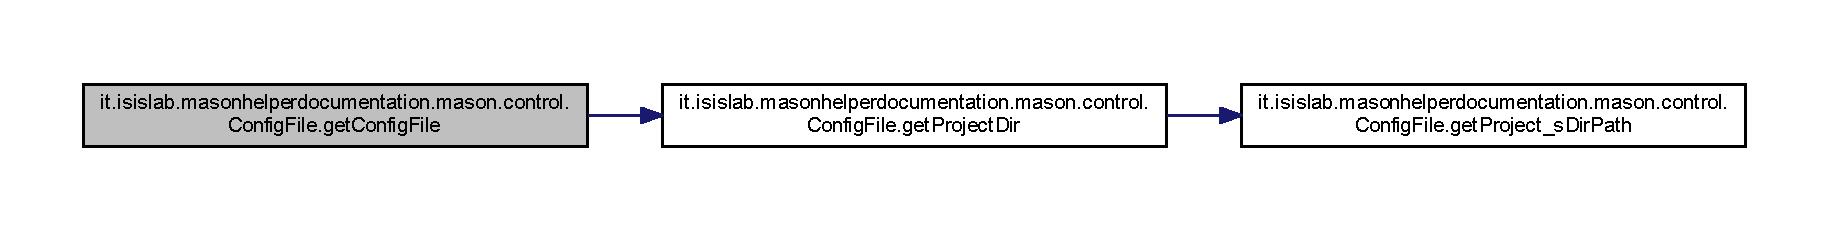
\includegraphics[width=350pt]{classit_1_1isislab_1_1masonhelperdocumentation_1_1mason_1_1control_1_1_config_file_ac533dd01e862be359ae060d278daf1ea_cgraph}
\end{center}
\end{figure}




Here is the caller graph for this function\-:
\nopagebreak
\begin{figure}[H]
\begin{center}
\leavevmode
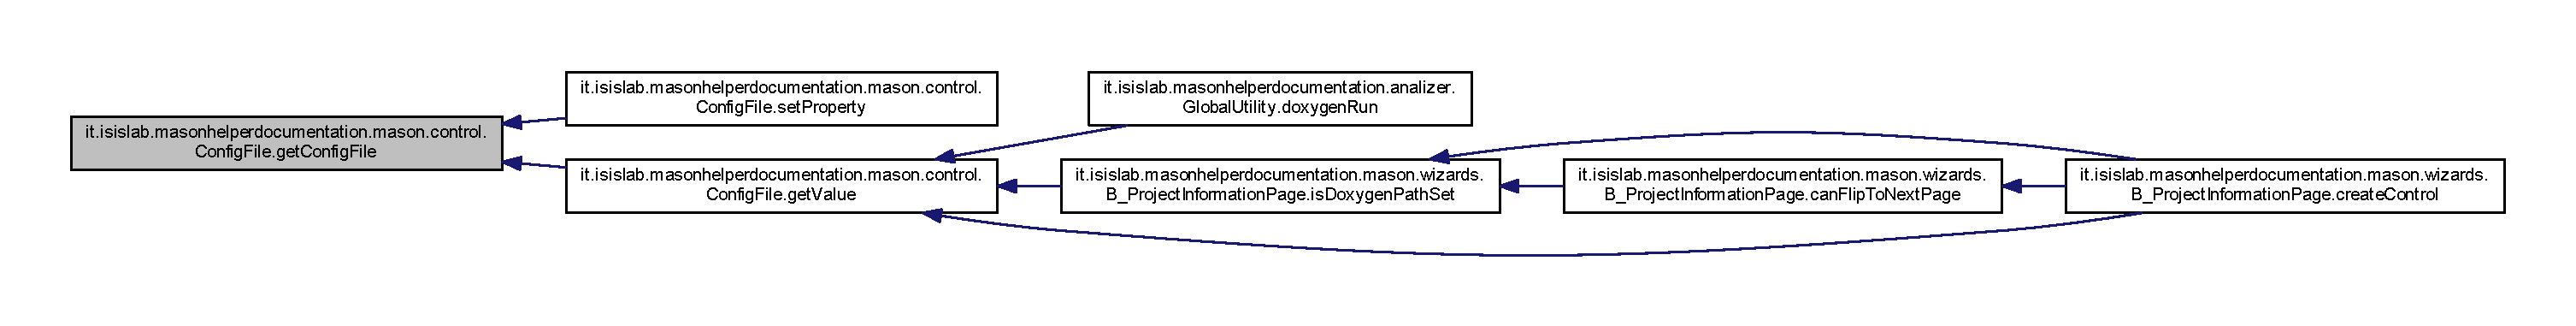
\includegraphics[width=350pt]{classit_1_1isislab_1_1masonhelperdocumentation_1_1mason_1_1control_1_1_config_file_ac533dd01e862be359ae060d278daf1ea_icgraph}
\end{center}
\end{figure}


\hypertarget{classit_1_1isislab_1_1masonhelperdocumentation_1_1mason_1_1control_1_1_config_file_afc023838475034a60185402e9cedbfba}{\index{it\-::isislab\-::masonhelperdocumentation\-::mason\-::control\-::\-Config\-File@{it\-::isislab\-::masonhelperdocumentation\-::mason\-::control\-::\-Config\-File}!get\-Dir@{get\-Dir}}
\index{get\-Dir@{get\-Dir}!it::isislab::masonhelperdocumentation::mason::control::ConfigFile@{it\-::isislab\-::masonhelperdocumentation\-::mason\-::control\-::\-Config\-File}}
\subsubsection[{get\-Dir}]{\setlength{\rightskip}{0pt plus 5cm}static String it.\-isislab.\-masonhelperdocumentation.\-mason.\-control.\-Config\-File.\-get\-Dir (
\begin{DoxyParamCaption}
{}
\end{DoxyParamCaption}
)\hspace{0.3cm}{\ttfamily [static]}}}\label{classit_1_1isislab_1_1masonhelperdocumentation_1_1mason_1_1control_1_1_config_file_afc023838475034a60185402e9cedbfba}
Return directory path; directory will be create (if does not exist) in disk root.

\begin{DoxyReturn}{Returns}

\end{DoxyReturn}

\begin{DoxyCode}
40                                   \{
41         String dirPath = File.separator + \hyperlink{classit_1_1isislab_1_1masonhelperdocumentation_1_1mason_1_1control_1_1_config_file_a7d8bbffdbfca146a398ed0bba454f347}{dirName} + GlobalUtility.getProjectAnalizer().
      getProjectName();
42         \textcolor{keyword}{new} File(dirPath).mkdir();
43         log.info(\textcolor{stringliteral}{"create/get dir: "} + dirPath);
44         \textcolor{keywordflow}{return} dirPath;
45     \}
\end{DoxyCode}


Here is the caller graph for this function\-:
\nopagebreak
\begin{figure}[H]
\begin{center}
\leavevmode
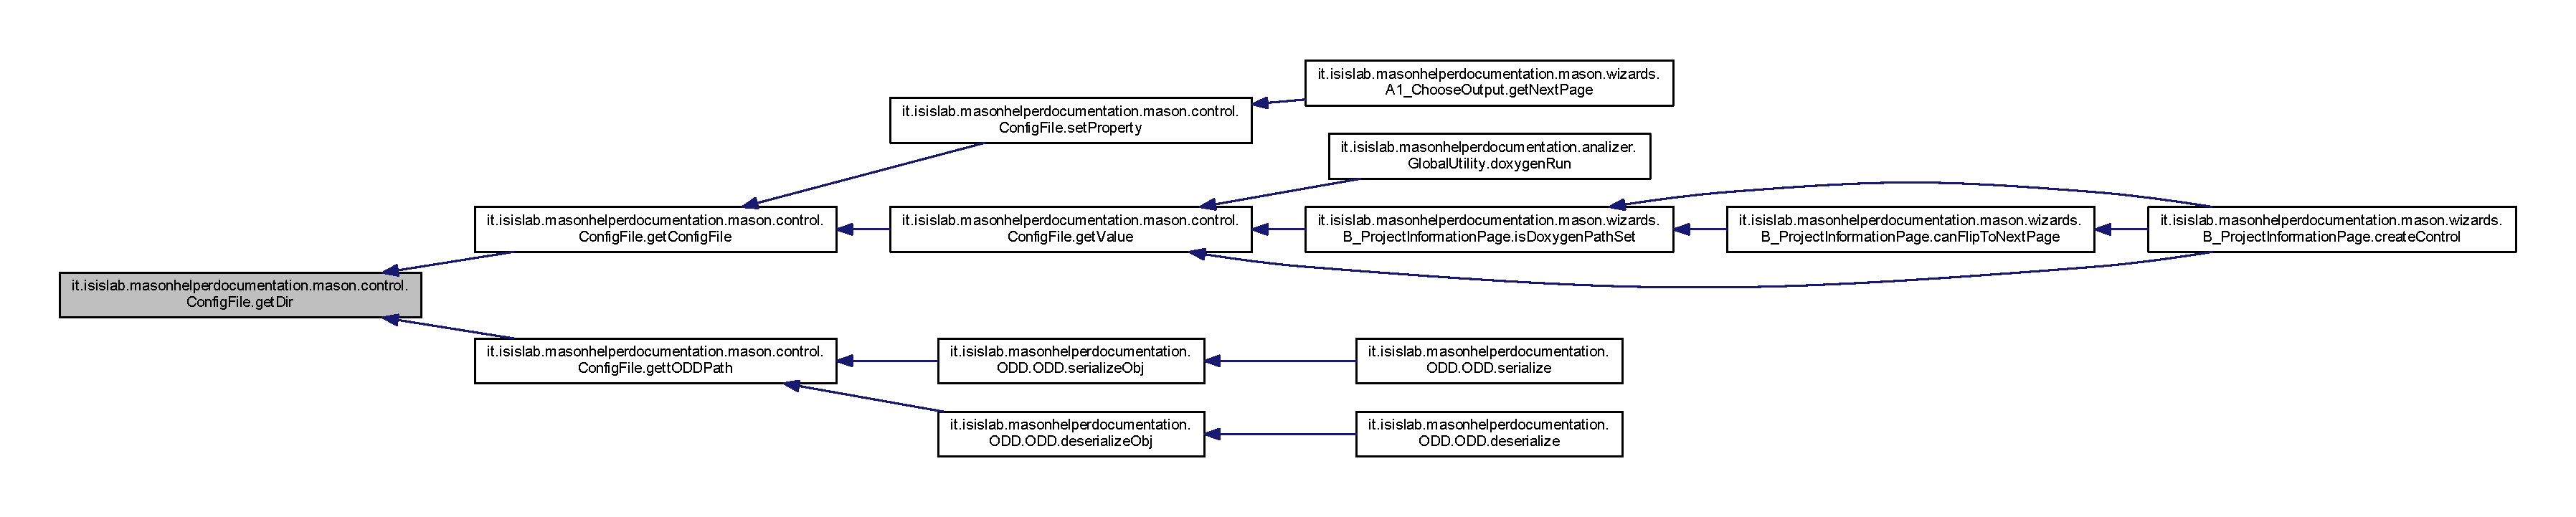
\includegraphics[width=350pt]{classit_1_1isislab_1_1masonhelperdocumentation_1_1mason_1_1control_1_1_config_file_afc023838475034a60185402e9cedbfba_icgraph}
\end{center}
\end{figure}


\hypertarget{classit_1_1isislab_1_1masonhelperdocumentation_1_1mason_1_1control_1_1_config_file_a066e1a4a3eb3969e1d59776ba39caac1}{\index{it\-::isislab\-::masonhelperdocumentation\-::mason\-::control\-::\-Config\-File@{it\-::isislab\-::masonhelperdocumentation\-::mason\-::control\-::\-Config\-File}!gett\-O\-D\-D\-Path@{gett\-O\-D\-D\-Path}}
\index{gett\-O\-D\-D\-Path@{gett\-O\-D\-D\-Path}!it::isislab::masonhelperdocumentation::mason::control::ConfigFile@{it\-::isislab\-::masonhelperdocumentation\-::mason\-::control\-::\-Config\-File}}
\subsubsection[{gett\-O\-D\-D\-Path}]{\setlength{\rightskip}{0pt plus 5cm}static String it.\-isislab.\-masonhelperdocumentation.\-mason.\-control.\-Config\-File.\-gett\-O\-D\-D\-Path (
\begin{DoxyParamCaption}
{}
\end{DoxyParamCaption}
)\hspace{0.3cm}{\ttfamily [static]}}}\label{classit_1_1isislab_1_1masonhelperdocumentation_1_1mason_1_1control_1_1_config_file_a066e1a4a3eb3969e1d59776ba39caac1}

\begin{DoxyCode}
143                                        \{
144         \textcolor{keywordflow}{return} \hyperlink{classit_1_1isislab_1_1masonhelperdocumentation_1_1mason_1_1control_1_1_config_file_afc023838475034a60185402e9cedbfba}{getDir}() + File.separator;
145     \}
\end{DoxyCode}


Here is the call graph for this function\-:
\nopagebreak
\begin{figure}[H]
\begin{center}
\leavevmode
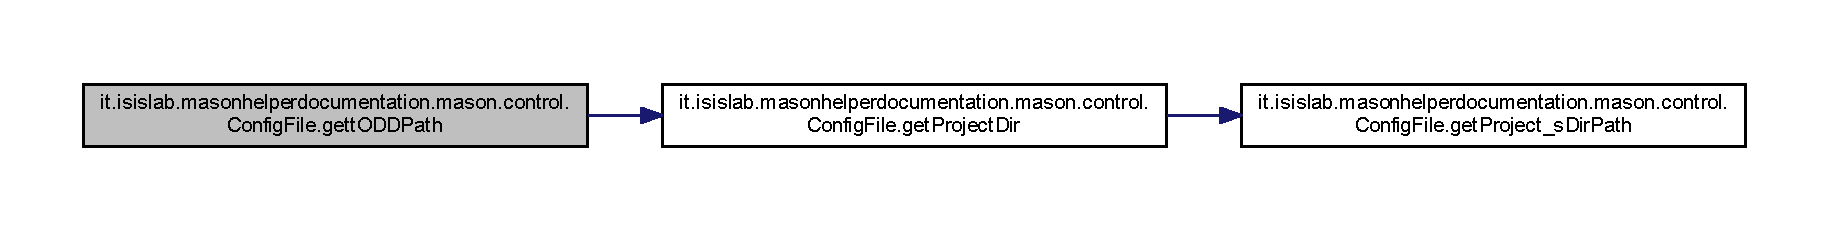
\includegraphics[width=350pt]{classit_1_1isislab_1_1masonhelperdocumentation_1_1mason_1_1control_1_1_config_file_a066e1a4a3eb3969e1d59776ba39caac1_cgraph}
\end{center}
\end{figure}




Here is the caller graph for this function\-:
\nopagebreak
\begin{figure}[H]
\begin{center}
\leavevmode
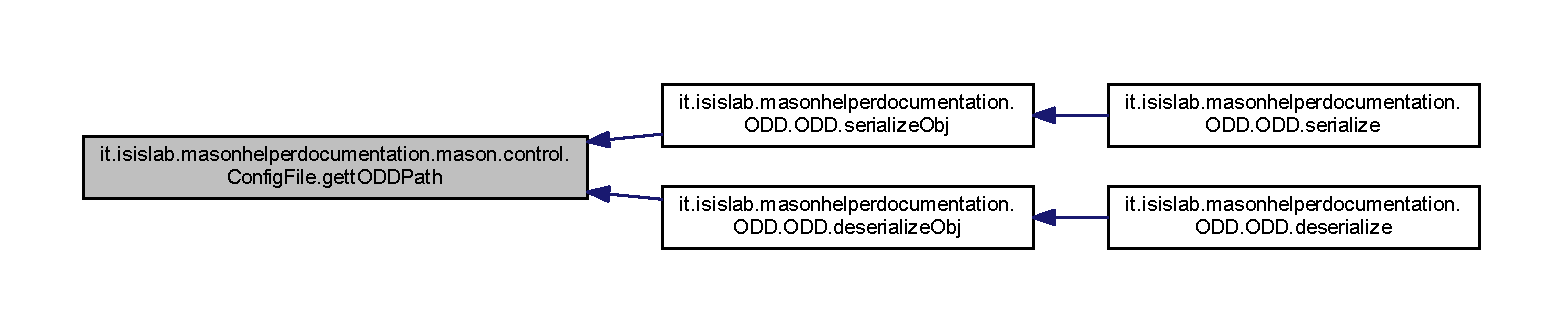
\includegraphics[width=350pt]{classit_1_1isislab_1_1masonhelperdocumentation_1_1mason_1_1control_1_1_config_file_a066e1a4a3eb3969e1d59776ba39caac1_icgraph}
\end{center}
\end{figure}


\hypertarget{classit_1_1isislab_1_1masonhelperdocumentation_1_1mason_1_1control_1_1_config_file_a7bcf08b34e48f0c5116d796d616113f0}{\index{it\-::isislab\-::masonhelperdocumentation\-::mason\-::control\-::\-Config\-File@{it\-::isislab\-::masonhelperdocumentation\-::mason\-::control\-::\-Config\-File}!get\-Value@{get\-Value}}
\index{get\-Value@{get\-Value}!it::isislab::masonhelperdocumentation::mason::control::ConfigFile@{it\-::isislab\-::masonhelperdocumentation\-::mason\-::control\-::\-Config\-File}}
\subsubsection[{get\-Value}]{\setlength{\rightskip}{0pt plus 5cm}static String it.\-isislab.\-masonhelperdocumentation.\-mason.\-control.\-Config\-File.\-get\-Value (
\begin{DoxyParamCaption}
\item[{String}]{key}
\end{DoxyParamCaption}
)\hspace{0.3cm}{\ttfamily [static]}}}\label{classit_1_1isislab_1_1masonhelperdocumentation_1_1mason_1_1control_1_1_config_file_a7bcf08b34e48f0c5116d796d616113f0}
Return the value associated to input key


\begin{DoxyParams}{Parameters}
{\em key} & \\
\hline
\end{DoxyParams}
\begin{DoxyReturn}{Returns}

\end{DoxyReturn}

\begin{DoxyCode}
118                                               \{
119         FileInputStream fstream = null;
120         DataInputStream in = null;
121 
122         \textcolor{keywordflow}{try} \{
123             fstream = \textcolor{keyword}{new} FileInputStream(\hyperlink{classit_1_1isislab_1_1masonhelperdocumentation_1_1mason_1_1control_1_1_config_file_ac533dd01e862be359ae060d278daf1ea}{getConfigFile}());
124             in = \textcolor{keyword}{new} DataInputStream(fstream);
125             BufferedReader br = \textcolor{keyword}{new} BufferedReader(\textcolor{keyword}{new} InputStreamReader(in));
126             String strLine;
127             \textcolor{keywordflow}{while} ((strLine = br.readLine()) != null) \{
128                 \textcolor{keywordflow}{if} (strLine.startsWith(key)) \{
129                     log.info(\textcolor{stringliteral}{"Get key: "} + key);
130                     \textcolor{keywordflow}{return} strLine.split(\textcolor{stringliteral}{"="})[1];
131                 \}
132             \}
133         \} \textcolor{keywordflow}{catch} (FileNotFoundException e) \{
134             log.severe(\textcolor{stringliteral}{"File not found: '"} + \hyperlink{classit_1_1isislab_1_1masonhelperdocumentation_1_1mason_1_1control_1_1_config_file_ac533dd01e862be359ae060d278daf1ea}{getConfigFile}() + \textcolor{stringliteral}{"' "}
135                     + e.getMessage());
136         \} \textcolor{keywordflow}{catch} (IOException e) \{
137             log.severe(\textcolor{stringliteral}{"Error reading file: '"} + \hyperlink{classit_1_1isislab_1_1masonhelperdocumentation_1_1mason_1_1control_1_1_config_file_ac533dd01e862be359ae060d278daf1ea}{getConfigFile}() + \textcolor{stringliteral}{"' "}
138                     + e.getMessage());
139         \}
140         \textcolor{keywordflow}{return} \textcolor{stringliteral}{""};
141     \}
\end{DoxyCode}


Here is the call graph for this function\-:
\nopagebreak
\begin{figure}[H]
\begin{center}
\leavevmode
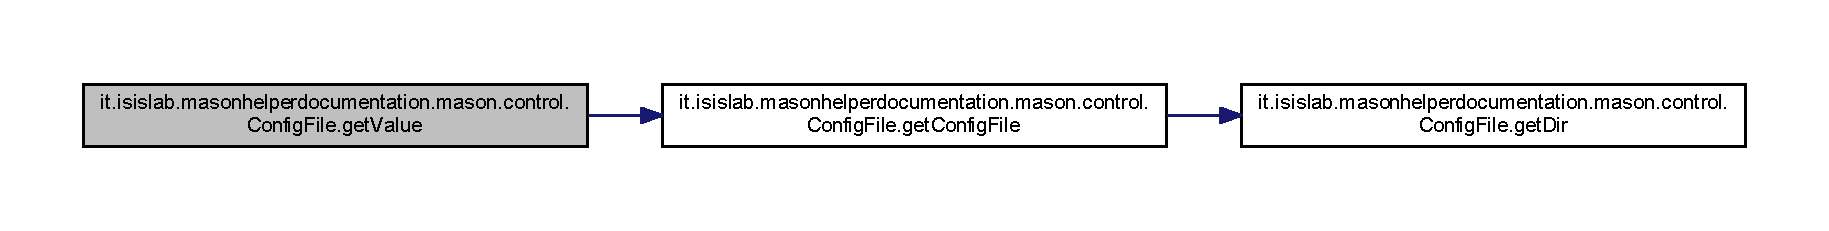
\includegraphics[width=350pt]{classit_1_1isislab_1_1masonhelperdocumentation_1_1mason_1_1control_1_1_config_file_a7bcf08b34e48f0c5116d796d616113f0_cgraph}
\end{center}
\end{figure}




Here is the caller graph for this function\-:
\nopagebreak
\begin{figure}[H]
\begin{center}
\leavevmode
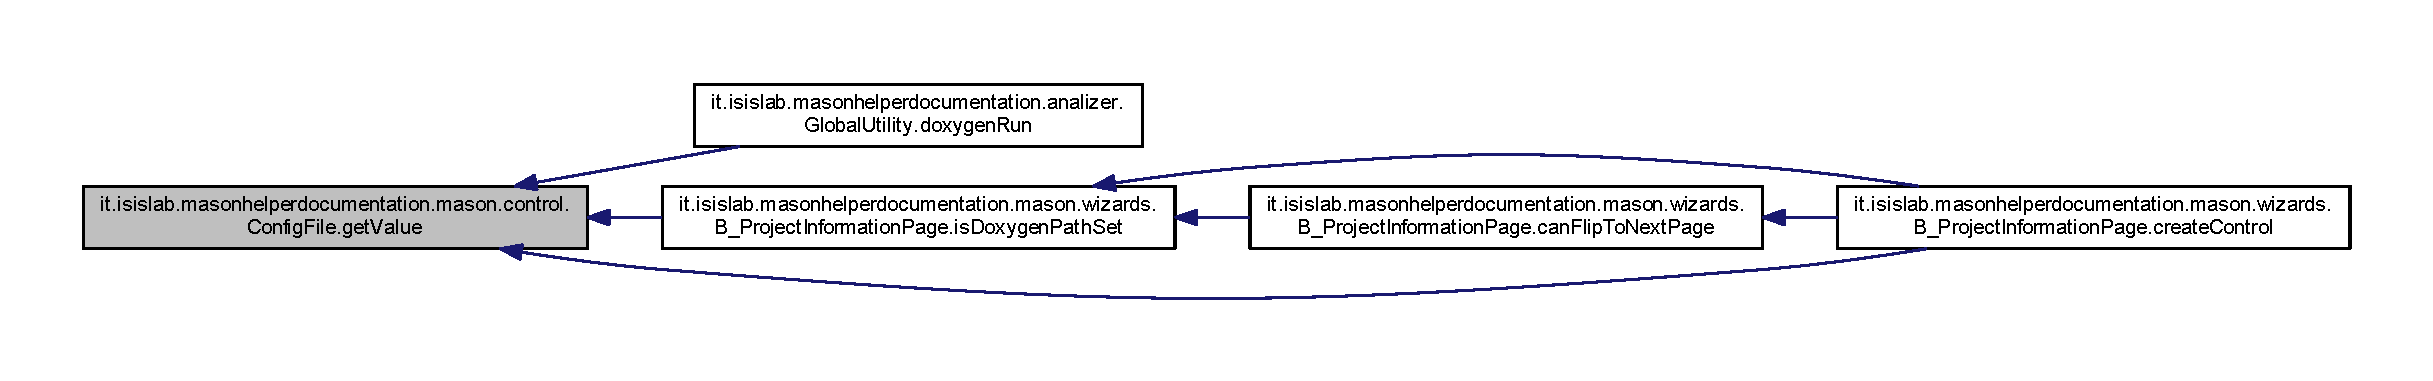
\includegraphics[width=350pt]{classit_1_1isislab_1_1masonhelperdocumentation_1_1mason_1_1control_1_1_config_file_a7bcf08b34e48f0c5116d796d616113f0_icgraph}
\end{center}
\end{figure}


\hypertarget{classit_1_1isislab_1_1masonhelperdocumentation_1_1mason_1_1control_1_1_config_file_a29d4bd9c148d1d7576cef7bcaf796172}{\index{it\-::isislab\-::masonhelperdocumentation\-::mason\-::control\-::\-Config\-File@{it\-::isislab\-::masonhelperdocumentation\-::mason\-::control\-::\-Config\-File}!set\-Property@{set\-Property}}
\index{set\-Property@{set\-Property}!it::isislab::masonhelperdocumentation::mason::control::ConfigFile@{it\-::isislab\-::masonhelperdocumentation\-::mason\-::control\-::\-Config\-File}}
\subsubsection[{set\-Property}]{\setlength{\rightskip}{0pt plus 5cm}static void it.\-isislab.\-masonhelperdocumentation.\-mason.\-control.\-Config\-File.\-set\-Property (
\begin{DoxyParamCaption}
\item[{String}]{key, }
\item[{String}]{value}
\end{DoxyParamCaption}
)\hspace{0.3cm}{\ttfamily [static]}}}\label{classit_1_1isislab_1_1masonhelperdocumentation_1_1mason_1_1control_1_1_config_file_a29d4bd9c148d1d7576cef7bcaf796172}
Set the key to value in \hyperlink{classit_1_1isislab_1_1masonhelperdocumentation_1_1mason_1_1control_1_1_config_file}{Config\-File} pointed by config\-File\-Path


\begin{DoxyParams}{Parameters}
{\em key} & \\
\hline
{\em value} & \\
\hline
\end{DoxyParams}

\begin{DoxyCode}
67                                                              \{
68         FileInputStream fstream = null;
69         DataInputStream in = null;
70         BufferedWriter out = null;
71         \textcolor{keywordtype}{boolean} propertySet = \textcolor{keyword}{false};
72 
73         \textcolor{keywordflow}{try} \{
74             fstream = \textcolor{keyword}{new} FileInputStream(\hyperlink{classit_1_1isislab_1_1masonhelperdocumentation_1_1mason_1_1control_1_1_config_file_ac533dd01e862be359ae060d278daf1ea}{getConfigFile}());
75             in = \textcolor{keyword}{new} DataInputStream(fstream);
76             BufferedReader br = \textcolor{keyword}{new} BufferedReader(\textcolor{keyword}{new} InputStreamReader(in));
77             String strLine;
78             StringBuilder fileContent = \textcolor{keyword}{new} StringBuilder();
79 
80             \textcolor{keywordflow}{while} ((strLine = br.readLine()) != null) \{
81                 \textcolor{keywordflow}{if} (strLine.startsWith(key)) \{
82                     fileContent.append(key + \textcolor{stringliteral}{"="} + value
83                             + System.getProperty(\textcolor{stringliteral}{"line.separator"}));
84                     propertySet = \textcolor{keyword}{true};
85                 \} \textcolor{keywordflow}{else} \{
86                     fileContent.append(strLine);
87                     fileContent.append(System.getProperty(\textcolor{stringliteral}{"line.separator"}));
88                 \}
89             \}
90             \textcolor{keywordflow}{if} (!propertySet) \{
91                 fileContent.append(key + \textcolor{stringliteral}{"="} + value);
92             \}
93 
94             FileWriter fstreamWrite = \textcolor{keyword}{new} FileWriter(\hyperlink{classit_1_1isislab_1_1masonhelperdocumentation_1_1mason_1_1control_1_1_config_file_ac533dd01e862be359ae060d278daf1ea}{getConfigFile}());
95             out = \textcolor{keyword}{new} BufferedWriter(fstreamWrite);
96             out.write(fileContent.toString());
97         \} \textcolor{keywordflow}{catch} (Exception e) \{
98             e.printStackTrace();
99         \} \textcolor{keywordflow}{finally} \{
100             \textcolor{keywordflow}{try} \{
101                 fstream.close();
102                 out.flush();
103                 out.close();
104                 in.close();
105             \} \textcolor{keywordflow}{catch} (IOException e) \{
106                 e.printStackTrace();
107             \}
108         \}
109         log.info(\textcolor{stringliteral}{"Set key: "} + key + \textcolor{stringliteral}{" to value: "} + value);
110     \}
\end{DoxyCode}


Here is the call graph for this function\-:
\nopagebreak
\begin{figure}[H]
\begin{center}
\leavevmode
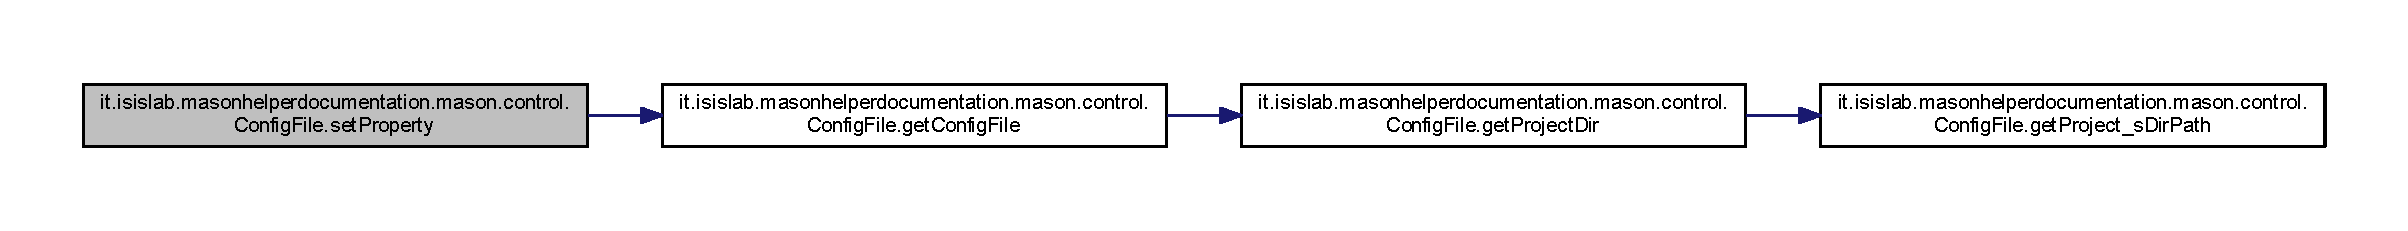
\includegraphics[width=350pt]{classit_1_1isislab_1_1masonhelperdocumentation_1_1mason_1_1control_1_1_config_file_a29d4bd9c148d1d7576cef7bcaf796172_cgraph}
\end{center}
\end{figure}




Here is the caller graph for this function\-:
\nopagebreak
\begin{figure}[H]
\begin{center}
\leavevmode
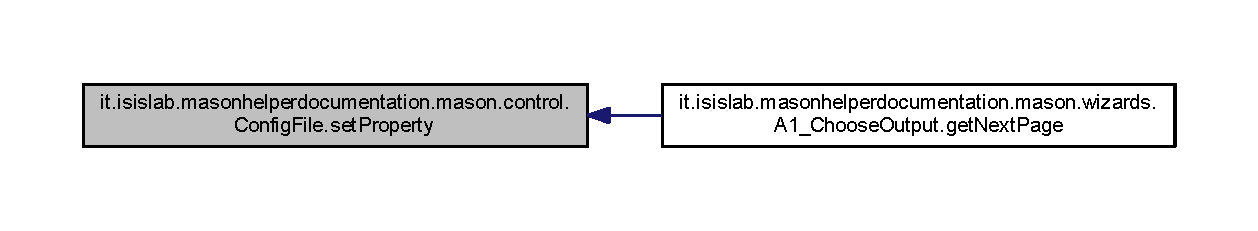
\includegraphics[width=350pt]{classit_1_1isislab_1_1masonhelperdocumentation_1_1mason_1_1control_1_1_config_file_a29d4bd9c148d1d7576cef7bcaf796172_icgraph}
\end{center}
\end{figure}




\subsection{Member Data Documentation}
\hypertarget{classit_1_1isislab_1_1masonhelperdocumentation_1_1mason_1_1control_1_1_config_file_a46a4e9d3359f002ff462e19976987878}{\index{it\-::isislab\-::masonhelperdocumentation\-::mason\-::control\-::\-Config\-File@{it\-::isislab\-::masonhelperdocumentation\-::mason\-::control\-::\-Config\-File}!config\-File\-Name@{config\-File\-Name}}
\index{config\-File\-Name@{config\-File\-Name}!it::isislab::masonhelperdocumentation::mason::control::ConfigFile@{it\-::isislab\-::masonhelperdocumentation\-::mason\-::control\-::\-Config\-File}}
\subsubsection[{config\-File\-Name}]{\setlength{\rightskip}{0pt plus 5cm}String it.\-isislab.\-masonhelperdocumentation.\-mason.\-control.\-Config\-File.\-config\-File\-Name = \char`\"{}config\-M\-A\-S\-O\-N\-Helper.\-dat\char`\"{}\hspace{0.3cm}{\ttfamily [static]}, {\ttfamily [private]}}}\label{classit_1_1isislab_1_1masonhelperdocumentation_1_1mason_1_1control_1_1_config_file_a46a4e9d3359f002ff462e19976987878}
\hypertarget{classit_1_1isislab_1_1masonhelperdocumentation_1_1mason_1_1control_1_1_config_file_a7d8bbffdbfca146a398ed0bba454f347}{\index{it\-::isislab\-::masonhelperdocumentation\-::mason\-::control\-::\-Config\-File@{it\-::isislab\-::masonhelperdocumentation\-::mason\-::control\-::\-Config\-File}!dir\-Name@{dir\-Name}}
\index{dir\-Name@{dir\-Name}!it::isislab::masonhelperdocumentation::mason::control::ConfigFile@{it\-::isislab\-::masonhelperdocumentation\-::mason\-::control\-::\-Config\-File}}
\subsubsection[{dir\-Name}]{\setlength{\rightskip}{0pt plus 5cm}String it.\-isislab.\-masonhelperdocumentation.\-mason.\-control.\-Config\-File.\-dir\-Name = \char`\"{}M\-A\-S\-O\-N\-Helper\-Documentation\-\_\-\char`\"{}\hspace{0.3cm}{\ttfamily [static]}, {\ttfamily [private]}}}\label{classit_1_1isislab_1_1masonhelperdocumentation_1_1mason_1_1control_1_1_config_file_a7d8bbffdbfca146a398ed0bba454f347}
\hypertarget{classit_1_1isislab_1_1masonhelperdocumentation_1_1mason_1_1control_1_1_config_file_a1e0cc7c39d846dcf3dd9def42f836e89}{\index{it\-::isislab\-::masonhelperdocumentation\-::mason\-::control\-::\-Config\-File@{it\-::isislab\-::masonhelperdocumentation\-::mason\-::control\-::\-Config\-File}!log@{log}}
\index{log@{log}!it::isislab::masonhelperdocumentation::mason::control::ConfigFile@{it\-::isislab\-::masonhelperdocumentation\-::mason\-::control\-::\-Config\-File}}
\subsubsection[{log}]{\setlength{\rightskip}{0pt plus 5cm}Logger it.\-isislab.\-masonhelperdocumentation.\-mason.\-control.\-Config\-File.\-log = Logger.\-get\-Logger(\char`\"{}global\char`\"{})\hspace{0.3cm}{\ttfamily [static]}, {\ttfamily [private]}}}\label{classit_1_1isislab_1_1masonhelperdocumentation_1_1mason_1_1control_1_1_config_file_a1e0cc7c39d846dcf3dd9def42f836e89}


The documentation for this class was generated from the following file\-:\begin{DoxyCompactItemize}
\item 
src/it/isislab/masonhelperdocumentation/mason/control/\hyperlink{_config_file_8java}{Config\-File.\-java}\end{DoxyCompactItemize}

\hypertarget{classit_1_1isislab_1_1masonhelperdocumentation_1_1mason_1_1wizards_1_1_d___agent_description_page}{\section{it.\-isislab.\-masonhelperdocumentation.\-mason.\-wizards.\-D\-\_\-\-Agent\-Description\-Page Class Reference}
\label{classit_1_1isislab_1_1masonhelperdocumentation_1_1mason_1_1wizards_1_1_d___agent_description_page}\index{it.\-isislab.\-masonhelperdocumentation.\-mason.\-wizards.\-D\-\_\-\-Agent\-Description\-Page@{it.\-isislab.\-masonhelperdocumentation.\-mason.\-wizards.\-D\-\_\-\-Agent\-Description\-Page}}
}


Inheritance diagram for it.\-isislab.\-masonhelperdocumentation.\-mason.\-wizards.\-D\-\_\-\-Agent\-Description\-Page\-:
\nopagebreak
\begin{figure}[H]
\begin{center}
\leavevmode
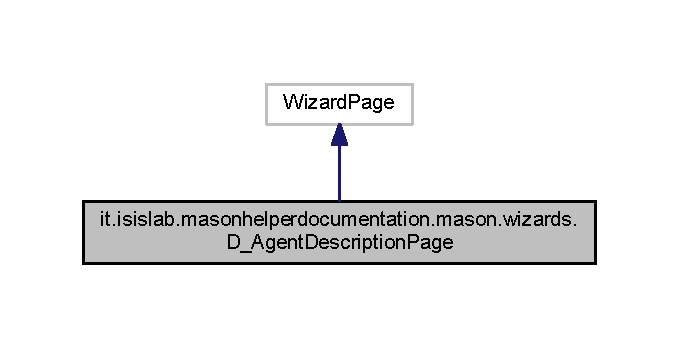
\includegraphics[width=326pt]{classit_1_1isislab_1_1masonhelperdocumentation_1_1mason_1_1wizards_1_1_d___agent_description_page__inherit__graph}
\end{center}
\end{figure}


Collaboration diagram for it.\-isislab.\-masonhelperdocumentation.\-mason.\-wizards.\-D\-\_\-\-Agent\-Description\-Page\-:
\nopagebreak
\begin{figure}[H]
\begin{center}
\leavevmode
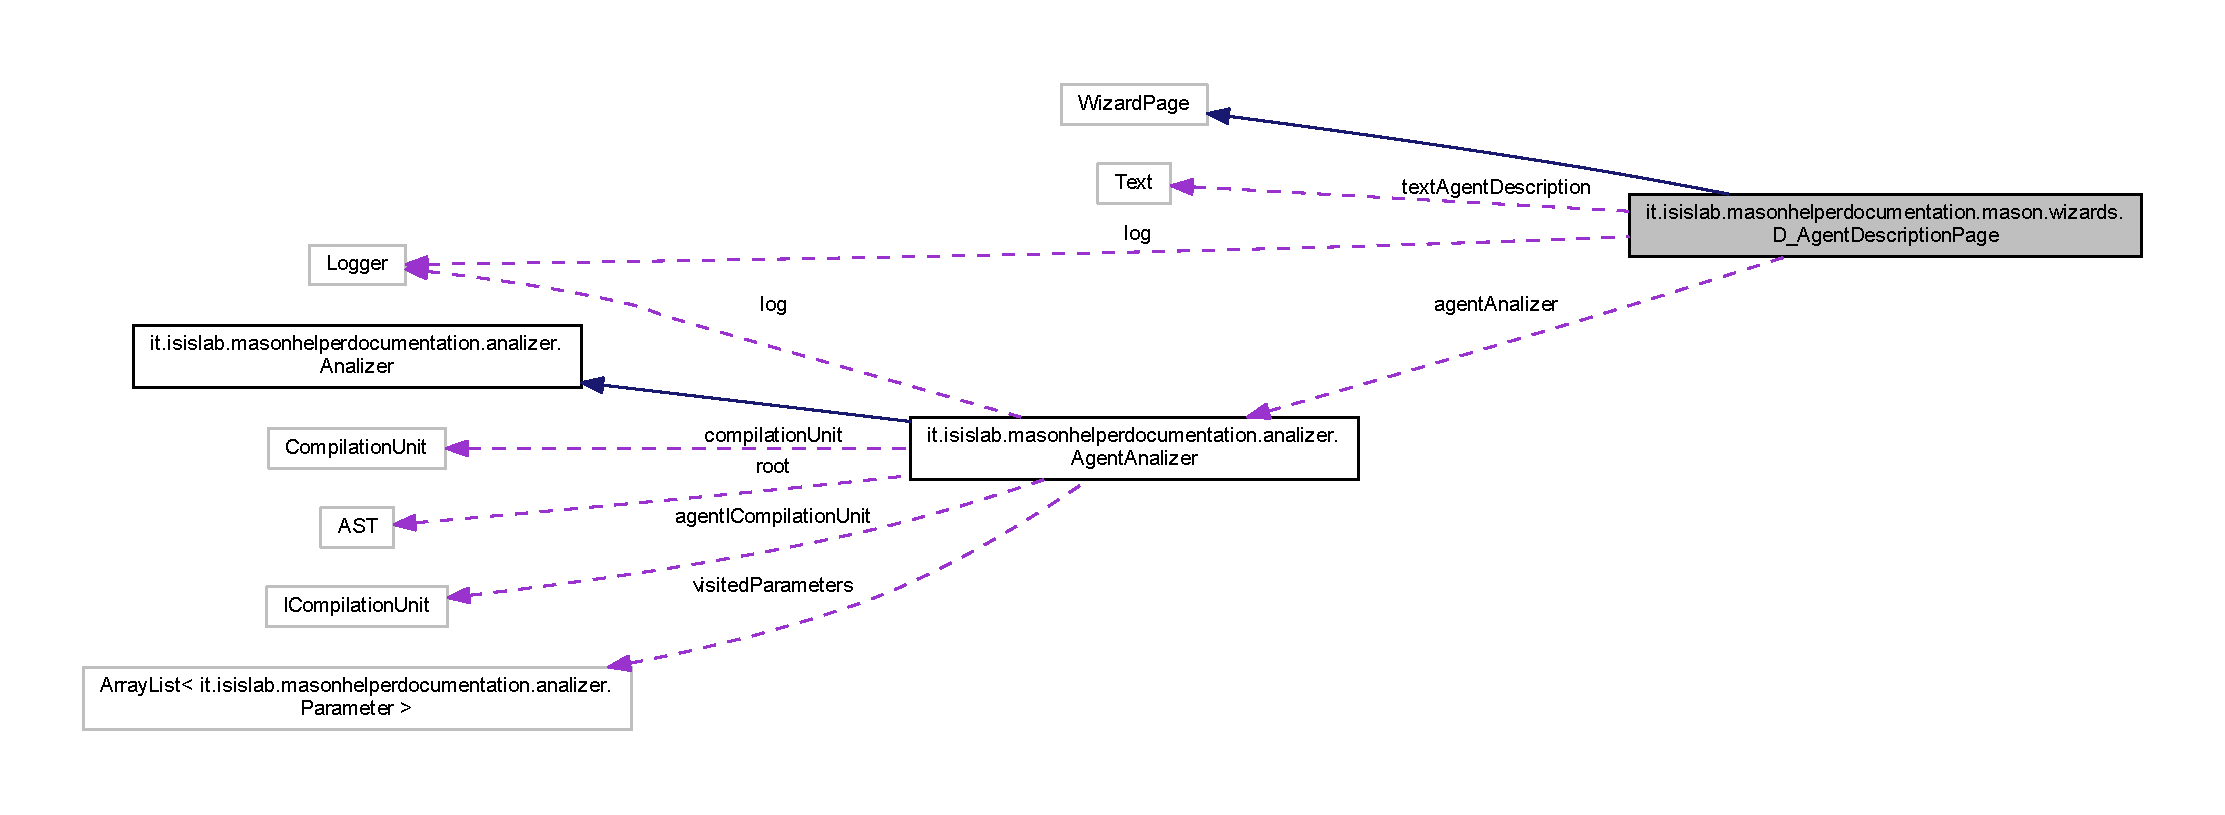
\includegraphics[width=350pt]{classit_1_1isislab_1_1masonhelperdocumentation_1_1mason_1_1wizards_1_1_d___agent_description_page__coll__graph}
\end{center}
\end{figure}
\subsection*{Public Member Functions}
\begin{DoxyCompactItemize}
\item 
\hyperlink{classit_1_1isislab_1_1masonhelperdocumentation_1_1mason_1_1wizards_1_1_d___agent_description_page_a16a7daf2bc98cdfde170aa29c028ba06}{D\-\_\-\-Agent\-Description\-Page} ()
\item 
void \hyperlink{classit_1_1isislab_1_1masonhelperdocumentation_1_1mason_1_1wizards_1_1_d___agent_description_page_a54ede11092f7bd9db6cc381862180450}{create\-Control} (Composite parent)
\item 
boolean \hyperlink{classit_1_1isislab_1_1masonhelperdocumentation_1_1mason_1_1wizards_1_1_d___agent_description_page_a2d82f96c4241c29fef9f80b28982f9a9}{can\-Flip\-To\-Next\-Page} ()
\item 
I\-Wizard\-Page \hyperlink{classit_1_1isislab_1_1masonhelperdocumentation_1_1mason_1_1wizards_1_1_d___agent_description_page_afc7ea33cd58dacc353ffd209027279fc}{get\-Next\-Page} ()
\end{DoxyCompactItemize}
\subsection*{Private Member Functions}
\begin{DoxyCompactItemize}
\item 
void \hyperlink{classit_1_1isislab_1_1masonhelperdocumentation_1_1mason_1_1wizards_1_1_d___agent_description_page_aa774dfe04837b0b796d9e292aa3935be}{get\-Old\-Information} ()
\end{DoxyCompactItemize}
\subsection*{Private Attributes}
\begin{DoxyCompactItemize}
\item 
\hyperlink{classit_1_1isislab_1_1masonhelperdocumentation_1_1analizer_1_1_agent_analizer}{Agent\-Analizer} \hyperlink{classit_1_1isislab_1_1masonhelperdocumentation_1_1mason_1_1wizards_1_1_d___agent_description_page_a2a9e05cc43fedb16d75050620d30f712}{agent\-Analizer}
\item 
Text \hyperlink{classit_1_1isislab_1_1masonhelperdocumentation_1_1mason_1_1wizards_1_1_d___agent_description_page_adeaf5a5649c9280ceb38690357c70a1b}{text\-Agent\-Description}
\end{DoxyCompactItemize}
\subsection*{Static Private Attributes}
\begin{DoxyCompactItemize}
\item 
static Logger \hyperlink{classit_1_1isislab_1_1masonhelperdocumentation_1_1mason_1_1wizards_1_1_d___agent_description_page_a52b31094ea4448637dde4a4fe4599a22}{log} = Logger.\-get\-Logger(\char`\"{}global\char`\"{})
\item 
static String \hyperlink{classit_1_1isislab_1_1masonhelperdocumentation_1_1mason_1_1wizards_1_1_d___agent_description_page_a8ba359bbeadb34933a78f865581fdf15}{page\-Description}
\end{DoxyCompactItemize}


\subsection{Detailed Description}
\begin{DoxyAuthor}{Author}
Romano Simone 0512101343 This page show agent description. 
\end{DoxyAuthor}


\subsection{Constructor \& Destructor Documentation}
\hypertarget{classit_1_1isislab_1_1masonhelperdocumentation_1_1mason_1_1wizards_1_1_d___agent_description_page_a16a7daf2bc98cdfde170aa29c028ba06}{\index{it\-::isislab\-::masonhelperdocumentation\-::mason\-::wizards\-::\-D\-\_\-\-Agent\-Description\-Page@{it\-::isislab\-::masonhelperdocumentation\-::mason\-::wizards\-::\-D\-\_\-\-Agent\-Description\-Page}!D\-\_\-\-Agent\-Description\-Page@{D\-\_\-\-Agent\-Description\-Page}}
\index{D\-\_\-\-Agent\-Description\-Page@{D\-\_\-\-Agent\-Description\-Page}!it::isislab::masonhelperdocumentation::mason::wizards::D_AgentDescriptionPage@{it\-::isislab\-::masonhelperdocumentation\-::mason\-::wizards\-::\-D\-\_\-\-Agent\-Description\-Page}}
\subsubsection[{D\-\_\-\-Agent\-Description\-Page}]{\setlength{\rightskip}{0pt plus 5cm}it.\-isislab.\-masonhelperdocumentation.\-mason.\-wizards.\-D\-\_\-\-Agent\-Description\-Page.\-D\-\_\-\-Agent\-Description\-Page (
\begin{DoxyParamCaption}
{}
\end{DoxyParamCaption}
)}}\label{classit_1_1isislab_1_1masonhelperdocumentation_1_1mason_1_1wizards_1_1_d___agent_description_page_a16a7daf2bc98cdfde170aa29c028ba06}
Constructor for Agent\-Description\-Page. 
\begin{DoxyParams}{Parameters}
{\em java\-Project} & \\
\hline
\end{DoxyParams}

\begin{DoxyCode}
49                                     \{
50         super(\textcolor{stringliteral}{"wizardPage"});
51         \hyperlink{classit_1_1isislab_1_1masonhelperdocumentation_1_1mason_1_1wizards_1_1_d___agent_description_page_a2a9e05cc43fedb16d75050620d30f712}{agentAnalizer} = GlobalUtility.getAgentAnalizer();
52         setTitle(\textcolor{stringliteral}{"2/7 - Entities, state variables, and scales\(\backslash\)n"} + \hyperlink{classit_1_1isislab_1_1masonhelperdocumentation_1_1mason_1_1wizards_1_1_d___agent_description_page_a2a9e05cc43fedb16d75050620d30f712}{agentAnalizer}.
      \hyperlink{classit_1_1isislab_1_1masonhelperdocumentation_1_1analizer_1_1_agent_analizer_ace466e16439878a851eb63d5a11ddf43}{getClassName}());
53         setDescription(\hyperlink{classit_1_1isislab_1_1masonhelperdocumentation_1_1mason_1_1wizards_1_1_d___agent_description_page_a8ba359bbeadb34933a78f865581fdf15}{pageDescription});
54     \}
\end{DoxyCode}


Here is the call graph for this function\-:
\nopagebreak
\begin{figure}[H]
\begin{center}
\leavevmode
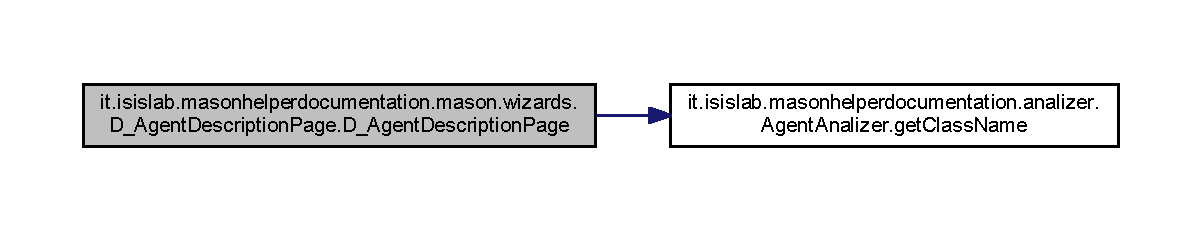
\includegraphics[width=350pt]{classit_1_1isislab_1_1masonhelperdocumentation_1_1mason_1_1wizards_1_1_d___agent_description_page_a16a7daf2bc98cdfde170aa29c028ba06_cgraph}
\end{center}
\end{figure}




\subsection{Member Function Documentation}
\hypertarget{classit_1_1isislab_1_1masonhelperdocumentation_1_1mason_1_1wizards_1_1_d___agent_description_page_a2d82f96c4241c29fef9f80b28982f9a9}{\index{it\-::isislab\-::masonhelperdocumentation\-::mason\-::wizards\-::\-D\-\_\-\-Agent\-Description\-Page@{it\-::isislab\-::masonhelperdocumentation\-::mason\-::wizards\-::\-D\-\_\-\-Agent\-Description\-Page}!can\-Flip\-To\-Next\-Page@{can\-Flip\-To\-Next\-Page}}
\index{can\-Flip\-To\-Next\-Page@{can\-Flip\-To\-Next\-Page}!it::isislab::masonhelperdocumentation::mason::wizards::D_AgentDescriptionPage@{it\-::isislab\-::masonhelperdocumentation\-::mason\-::wizards\-::\-D\-\_\-\-Agent\-Description\-Page}}
\subsubsection[{can\-Flip\-To\-Next\-Page}]{\setlength{\rightskip}{0pt plus 5cm}boolean it.\-isislab.\-masonhelperdocumentation.\-mason.\-wizards.\-D\-\_\-\-Agent\-Description\-Page.\-can\-Flip\-To\-Next\-Page (
\begin{DoxyParamCaption}
{}
\end{DoxyParamCaption}
)}}\label{classit_1_1isislab_1_1masonhelperdocumentation_1_1mason_1_1wizards_1_1_d___agent_description_page_a2d82f96c4241c29fef9f80b28982f9a9}

\begin{DoxyCode}
85                                        \{
86         \textcolor{keywordflow}{return} \textcolor{keyword}{true};
87     \}
\end{DoxyCode}
\hypertarget{classit_1_1isislab_1_1masonhelperdocumentation_1_1mason_1_1wizards_1_1_d___agent_description_page_a54ede11092f7bd9db6cc381862180450}{\index{it\-::isislab\-::masonhelperdocumentation\-::mason\-::wizards\-::\-D\-\_\-\-Agent\-Description\-Page@{it\-::isislab\-::masonhelperdocumentation\-::mason\-::wizards\-::\-D\-\_\-\-Agent\-Description\-Page}!create\-Control@{create\-Control}}
\index{create\-Control@{create\-Control}!it::isislab::masonhelperdocumentation::mason::wizards::D_AgentDescriptionPage@{it\-::isislab\-::masonhelperdocumentation\-::mason\-::wizards\-::\-D\-\_\-\-Agent\-Description\-Page}}
\subsubsection[{create\-Control}]{\setlength{\rightskip}{0pt plus 5cm}void it.\-isislab.\-masonhelperdocumentation.\-mason.\-wizards.\-D\-\_\-\-Agent\-Description\-Page.\-create\-Control (
\begin{DoxyParamCaption}
\item[{Composite}]{parent}
\end{DoxyParamCaption}
)}}\label{classit_1_1isislab_1_1masonhelperdocumentation_1_1mason_1_1wizards_1_1_d___agent_description_page_a54ede11092f7bd9db6cc381862180450}

\begin{DoxyCode}
56                                                 \{
57         Composite container = \textcolor{keyword}{new} Composite(parent, SWT.NULL);
58         setControl(container);
59         container.setLayout(\textcolor{keyword}{new} GridLayout(1,\textcolor{keyword}{true}));
60         
61         Label lblAgentDefinition = \textcolor{keyword}{new} Label(container, SWT.NONE);
62         GridData gd\_lblAgentDefinition = \textcolor{keyword}{new} GridData(SWT.CENTER, SWT.CENTER, \textcolor{keyword}{false}, \textcolor{keyword}{false}, 1, 1);
63         gd\_lblAgentDefinition.widthHint = 567;
64         lblAgentDefinition.setLayoutData(gd\_lblAgentDefinition);
65         lblAgentDefinition.setText(\textcolor{stringliteral}{"Description for entities: "} + agentAnalizer.getClassName());
66 
67         \hyperlink{classit_1_1isislab_1_1masonhelperdocumentation_1_1mason_1_1wizards_1_1_d___agent_description_page_adeaf5a5649c9280ceb38690357c70a1b}{textAgentDescription} = \textcolor{keyword}{new} Text(container, SWT.BORDER | SWT.MULTI);
68         GridData gd\_text = \textcolor{keyword}{new} GridData(SWT.FILL, SWT.CENTER, \textcolor{keyword}{true}, \textcolor{keyword}{false}, 1, 1);
69         gd\_text.heightHint = 93;
70         textAgentDescription.setLayoutData(gd\_text);
71 
72         
73         \hyperlink{classit_1_1isislab_1_1masonhelperdocumentation_1_1mason_1_1wizards_1_1_d___agent_description_page_aa774dfe04837b0b796d9e292aa3935be}{getOldInformation}();
74         
75     \}
\end{DoxyCode}


Here is the call graph for this function\-:
\nopagebreak
\begin{figure}[H]
\begin{center}
\leavevmode
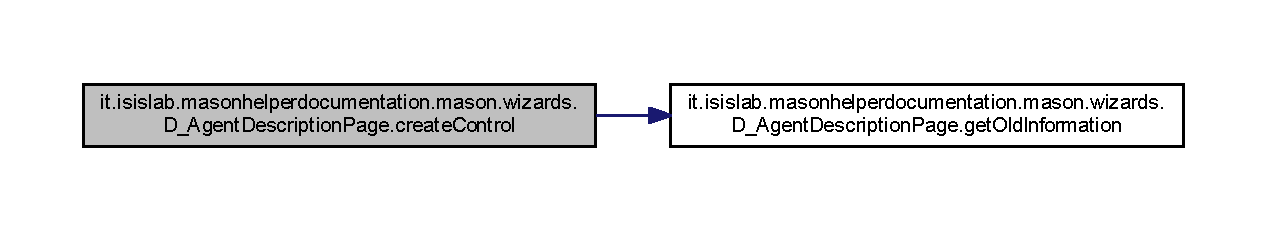
\includegraphics[width=350pt]{classit_1_1isislab_1_1masonhelperdocumentation_1_1mason_1_1wizards_1_1_d___agent_description_page_a54ede11092f7bd9db6cc381862180450_cgraph}
\end{center}
\end{figure}


\hypertarget{classit_1_1isislab_1_1masonhelperdocumentation_1_1mason_1_1wizards_1_1_d___agent_description_page_afc7ea33cd58dacc353ffd209027279fc}{\index{it\-::isislab\-::masonhelperdocumentation\-::mason\-::wizards\-::\-D\-\_\-\-Agent\-Description\-Page@{it\-::isislab\-::masonhelperdocumentation\-::mason\-::wizards\-::\-D\-\_\-\-Agent\-Description\-Page}!get\-Next\-Page@{get\-Next\-Page}}
\index{get\-Next\-Page@{get\-Next\-Page}!it::isislab::masonhelperdocumentation::mason::wizards::D_AgentDescriptionPage@{it\-::isislab\-::masonhelperdocumentation\-::mason\-::wizards\-::\-D\-\_\-\-Agent\-Description\-Page}}
\subsubsection[{get\-Next\-Page}]{\setlength{\rightskip}{0pt plus 5cm}I\-Wizard\-Page it.\-isislab.\-masonhelperdocumentation.\-mason.\-wizards.\-D\-\_\-\-Agent\-Description\-Page.\-get\-Next\-Page (
\begin{DoxyParamCaption}
{}
\end{DoxyParamCaption}
)}}\label{classit_1_1isislab_1_1masonhelperdocumentation_1_1mason_1_1wizards_1_1_d___agent_description_page_afc7ea33cd58dacc353ffd209027279fc}
Add this agent to Entities list (entities represent the Entites of \hyperlink{namespaceit_1_1isislab_1_1masonhelperdocumentation_1_1_o_d_d}{O\-D\-D} protocol -\/ section 2) 
\begin{DoxyParams}{Parameters}
{\em agent\-Analizer} & \\
\hline
\end{DoxyParams}

\begin{DoxyCode}
89                                     \{ 
90         \textcolor{comment}{//store new autogenerated information}
91         agentAnalizer.setClassDescription(textAgentDescription.getText());
97         ODD.addEntity(\textcolor{keyword}{new} Entity(\hyperlink{classit_1_1isislab_1_1masonhelperdocumentation_1_1mason_1_1wizards_1_1_d___agent_description_page_a2a9e05cc43fedb16d75050620d30f712}{agentAnalizer}.\hyperlink{classit_1_1isislab_1_1masonhelperdocumentation_1_1analizer_1_1_agent_analizer_ace466e16439878a851eb63d5a11ddf43}{getClassName}(), 
      textAgentDescription.getText()));   
98         \textcolor{keywordflow}{if} (\hyperlink{classit_1_1isislab_1_1masonhelperdocumentation_1_1mason_1_1wizards_1_1_d___agent_description_page_a2a9e05cc43fedb16d75050620d30f712}{agentAnalizer}.\hyperlink{classit_1_1isislab_1_1masonhelperdocumentation_1_1analizer_1_1_agent_analizer_aa2e85956f4a23176c398294cf02d859d}{getPositionsParameter}().size() != 0)\{
99             E\_AgentPositionPage nextPage = \textcolor{keyword}{new} E\_AgentPositionPage();
100             ((MASONDocumentationWizard) super.getWizard()).addPage(nextPage); 
101             \textcolor{keywordflow}{return} nextPage; 
102         \}
103         \textcolor{keywordflow}{else}\{
104             F\_AgentVariablesPage nextPage = \textcolor{keyword}{new} F\_AgentVariablesPage();
105             ((MASONDocumentationWizard) super.getWizard()).addPage(nextPage);
106             \textcolor{keywordflow}{return} nextPage;
107         \}
108     \}
\end{DoxyCode}


Here is the call graph for this function\-:
\nopagebreak
\begin{figure}[H]
\begin{center}
\leavevmode
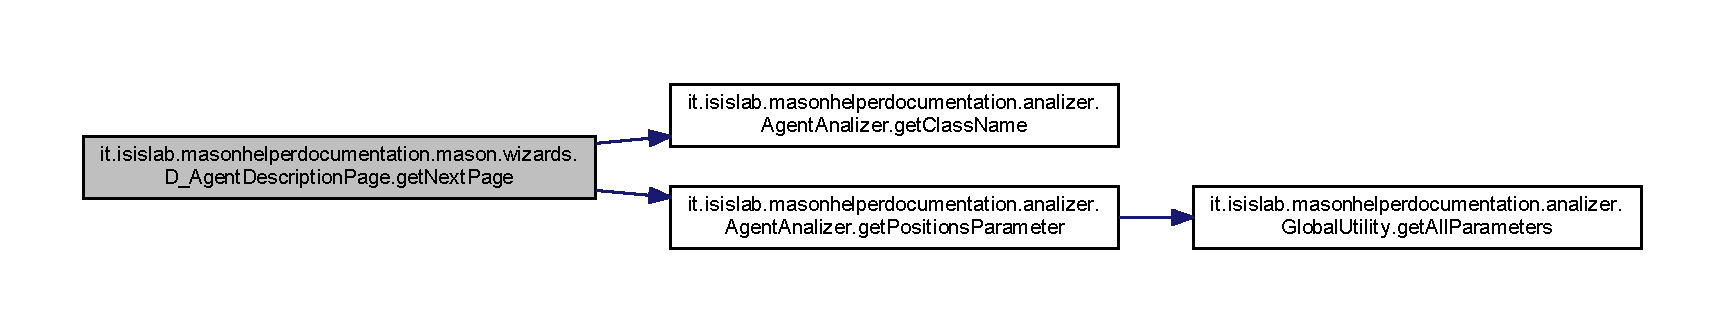
\includegraphics[width=350pt]{classit_1_1isislab_1_1masonhelperdocumentation_1_1mason_1_1wizards_1_1_d___agent_description_page_afc7ea33cd58dacc353ffd209027279fc_cgraph}
\end{center}
\end{figure}


\hypertarget{classit_1_1isislab_1_1masonhelperdocumentation_1_1mason_1_1wizards_1_1_d___agent_description_page_aa774dfe04837b0b796d9e292aa3935be}{\index{it\-::isislab\-::masonhelperdocumentation\-::mason\-::wizards\-::\-D\-\_\-\-Agent\-Description\-Page@{it\-::isislab\-::masonhelperdocumentation\-::mason\-::wizards\-::\-D\-\_\-\-Agent\-Description\-Page}!get\-Old\-Information@{get\-Old\-Information}}
\index{get\-Old\-Information@{get\-Old\-Information}!it::isislab::masonhelperdocumentation::mason::wizards::D_AgentDescriptionPage@{it\-::isislab\-::masonhelperdocumentation\-::mason\-::wizards\-::\-D\-\_\-\-Agent\-Description\-Page}}
\subsubsection[{get\-Old\-Information}]{\setlength{\rightskip}{0pt plus 5cm}void it.\-isislab.\-masonhelperdocumentation.\-mason.\-wizards.\-D\-\_\-\-Agent\-Description\-Page.\-get\-Old\-Information (
\begin{DoxyParamCaption}
{}
\end{DoxyParamCaption}
)\hspace{0.3cm}{\ttfamily [private]}}}\label{classit_1_1isislab_1_1masonhelperdocumentation_1_1mason_1_1wizards_1_1_d___agent_description_page_aa774dfe04837b0b796d9e292aa3935be}

\begin{DoxyCode}
78                                      \{
79         Entity agent = ODD.getEntity(agentAnalizer.getClassName());
80         \textcolor{keywordflow}{if} (agent != null)
81             textAgentDescription.setText(agent.getDescription());
82     \}
\end{DoxyCode}


Here is the caller graph for this function\-:
\nopagebreak
\begin{figure}[H]
\begin{center}
\leavevmode
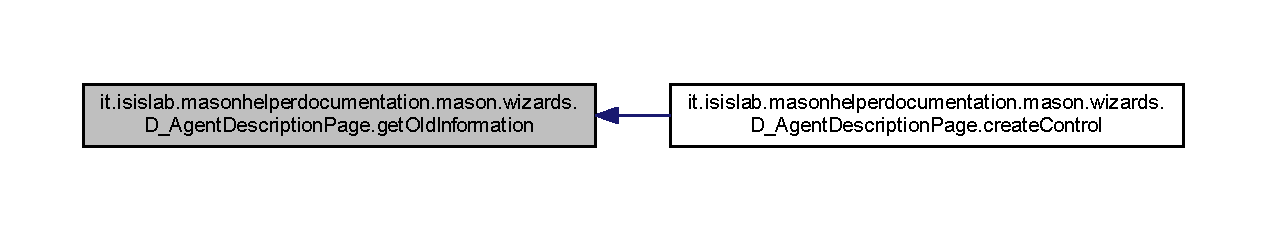
\includegraphics[width=350pt]{classit_1_1isislab_1_1masonhelperdocumentation_1_1mason_1_1wizards_1_1_d___agent_description_page_aa774dfe04837b0b796d9e292aa3935be_icgraph}
\end{center}
\end{figure}




\subsection{Member Data Documentation}
\hypertarget{classit_1_1isislab_1_1masonhelperdocumentation_1_1mason_1_1wizards_1_1_d___agent_description_page_a2a9e05cc43fedb16d75050620d30f712}{\index{it\-::isislab\-::masonhelperdocumentation\-::mason\-::wizards\-::\-D\-\_\-\-Agent\-Description\-Page@{it\-::isislab\-::masonhelperdocumentation\-::mason\-::wizards\-::\-D\-\_\-\-Agent\-Description\-Page}!agent\-Analizer@{agent\-Analizer}}
\index{agent\-Analizer@{agent\-Analizer}!it::isislab::masonhelperdocumentation::mason::wizards::D_AgentDescriptionPage@{it\-::isislab\-::masonhelperdocumentation\-::mason\-::wizards\-::\-D\-\_\-\-Agent\-Description\-Page}}
\subsubsection[{agent\-Analizer}]{\setlength{\rightskip}{0pt plus 5cm}{\bf Agent\-Analizer} it.\-isislab.\-masonhelperdocumentation.\-mason.\-wizards.\-D\-\_\-\-Agent\-Description\-Page.\-agent\-Analizer\hspace{0.3cm}{\ttfamily [private]}}}\label{classit_1_1isislab_1_1masonhelperdocumentation_1_1mason_1_1wizards_1_1_d___agent_description_page_a2a9e05cc43fedb16d75050620d30f712}
\hypertarget{classit_1_1isislab_1_1masonhelperdocumentation_1_1mason_1_1wizards_1_1_d___agent_description_page_a52b31094ea4448637dde4a4fe4599a22}{\index{it\-::isislab\-::masonhelperdocumentation\-::mason\-::wizards\-::\-D\-\_\-\-Agent\-Description\-Page@{it\-::isislab\-::masonhelperdocumentation\-::mason\-::wizards\-::\-D\-\_\-\-Agent\-Description\-Page}!log@{log}}
\index{log@{log}!it::isislab::masonhelperdocumentation::mason::wizards::D_AgentDescriptionPage@{it\-::isislab\-::masonhelperdocumentation\-::mason\-::wizards\-::\-D\-\_\-\-Agent\-Description\-Page}}
\subsubsection[{log}]{\setlength{\rightskip}{0pt plus 5cm}Logger it.\-isislab.\-masonhelperdocumentation.\-mason.\-wizards.\-D\-\_\-\-Agent\-Description\-Page.\-log = Logger.\-get\-Logger(\char`\"{}global\char`\"{})\hspace{0.3cm}{\ttfamily [static]}, {\ttfamily [private]}}}\label{classit_1_1isislab_1_1masonhelperdocumentation_1_1mason_1_1wizards_1_1_d___agent_description_page_a52b31094ea4448637dde4a4fe4599a22}
\hypertarget{classit_1_1isislab_1_1masonhelperdocumentation_1_1mason_1_1wizards_1_1_d___agent_description_page_a8ba359bbeadb34933a78f865581fdf15}{\index{it\-::isislab\-::masonhelperdocumentation\-::mason\-::wizards\-::\-D\-\_\-\-Agent\-Description\-Page@{it\-::isislab\-::masonhelperdocumentation\-::mason\-::wizards\-::\-D\-\_\-\-Agent\-Description\-Page}!page\-Description@{page\-Description}}
\index{page\-Description@{page\-Description}!it::isislab::masonhelperdocumentation::mason::wizards::D_AgentDescriptionPage@{it\-::isislab\-::masonhelperdocumentation\-::mason\-::wizards\-::\-D\-\_\-\-Agent\-Description\-Page}}
\subsubsection[{page\-Description}]{\setlength{\rightskip}{0pt plus 5cm}String it.\-isislab.\-masonhelperdocumentation.\-mason.\-wizards.\-D\-\_\-\-Agent\-Description\-Page.\-page\-Description\hspace{0.3cm}{\ttfamily [static]}, {\ttfamily [private]}}}\label{classit_1_1isislab_1_1masonhelperdocumentation_1_1mason_1_1wizards_1_1_d___agent_description_page_a8ba359bbeadb34933a78f865581fdf15}
{\bfseries Initial value\-:}
\begin{DoxyCode}
= \textcolor{stringliteral}{"What kinds of entities are in the model?\(\backslash\)n"}
                                          + \textcolor{stringliteral}{"By what state variables, or attributes, are these entities
       characterized?\(\backslash\)n"}
                                          + \textcolor{stringliteral}{"What are the temporal and spatial resolutions and extents of
       the model?"}
\end{DoxyCode}
\hypertarget{classit_1_1isislab_1_1masonhelperdocumentation_1_1mason_1_1wizards_1_1_d___agent_description_page_adeaf5a5649c9280ceb38690357c70a1b}{\index{it\-::isislab\-::masonhelperdocumentation\-::mason\-::wizards\-::\-D\-\_\-\-Agent\-Description\-Page@{it\-::isislab\-::masonhelperdocumentation\-::mason\-::wizards\-::\-D\-\_\-\-Agent\-Description\-Page}!text\-Agent\-Description@{text\-Agent\-Description}}
\index{text\-Agent\-Description@{text\-Agent\-Description}!it::isislab::masonhelperdocumentation::mason::wizards::D_AgentDescriptionPage@{it\-::isislab\-::masonhelperdocumentation\-::mason\-::wizards\-::\-D\-\_\-\-Agent\-Description\-Page}}
\subsubsection[{text\-Agent\-Description}]{\setlength{\rightskip}{0pt plus 5cm}Text it.\-isislab.\-masonhelperdocumentation.\-mason.\-wizards.\-D\-\_\-\-Agent\-Description\-Page.\-text\-Agent\-Description\hspace{0.3cm}{\ttfamily [private]}}}\label{classit_1_1isislab_1_1masonhelperdocumentation_1_1mason_1_1wizards_1_1_d___agent_description_page_adeaf5a5649c9280ceb38690357c70a1b}


The documentation for this class was generated from the following file\-:\begin{DoxyCompactItemize}
\item 
git/masonhelperdocumentation/src/it/isislab/masonhelperdocumentation/mason/wizards/\hyperlink{_d___agent_description_page_8java}{D\-\_\-\-Agent\-Description\-Page.\-java}\end{DoxyCompactItemize}

\hypertarget{classit_1_1isislab_1_1masonhelperdocumentation_1_1_o_d_d_1_1_design_concepts}{\section{it.\-isislab.\-masonhelperdocumentation.\-O\-D\-D.\-Design\-Concepts Class Reference}
\label{classit_1_1isislab_1_1masonhelperdocumentation_1_1_o_d_d_1_1_design_concepts}\index{it.\-isislab.\-masonhelperdocumentation.\-O\-D\-D.\-Design\-Concepts@{it.\-isislab.\-masonhelperdocumentation.\-O\-D\-D.\-Design\-Concepts}}
}


Inheritance diagram for it.\-isislab.\-masonhelperdocumentation.\-O\-D\-D.\-Design\-Concepts\-:
\nopagebreak
\begin{figure}[H]
\begin{center}
\leavevmode
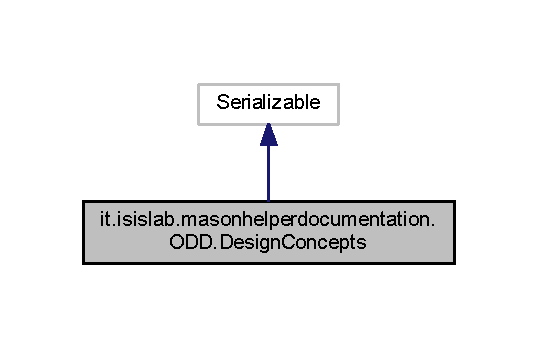
\includegraphics[width=258pt]{classit_1_1isislab_1_1masonhelperdocumentation_1_1_o_d_d_1_1_design_concepts__inherit__graph}
\end{center}
\end{figure}


Collaboration diagram for it.\-isislab.\-masonhelperdocumentation.\-O\-D\-D.\-Design\-Concepts\-:
\nopagebreak
\begin{figure}[H]
\begin{center}
\leavevmode
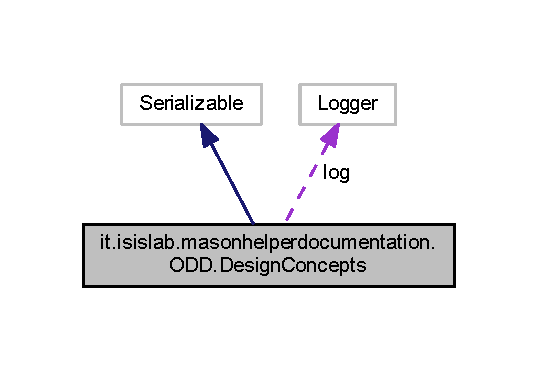
\includegraphics[width=258pt]{classit_1_1isislab_1_1masonhelperdocumentation_1_1_o_d_d_1_1_design_concepts__coll__graph}
\end{center}
\end{figure}
\subsection*{Public Member Functions}
\begin{DoxyCompactItemize}
\item 
String \hyperlink{classit_1_1isislab_1_1masonhelperdocumentation_1_1_o_d_d_1_1_design_concepts_adb4dd71450f8f1b5ad54a68b63a8662b}{get\-Auto\-Basic\-Principles} ()
\item 
void \hyperlink{classit_1_1isislab_1_1masonhelperdocumentation_1_1_o_d_d_1_1_design_concepts_a19c4d24937bd3d86da8b59308b47f3ba}{set\-Auto\-Basic\-Principles} (String \hyperlink{classit_1_1isislab_1_1masonhelperdocumentation_1_1_o_d_d_1_1_design_concepts_aa5a0af5b9002ffab0de5e9a219b39f8d}{auto\-Basic\-Principles})
\item 
String \hyperlink{classit_1_1isislab_1_1masonhelperdocumentation_1_1_o_d_d_1_1_design_concepts_ad4aa2370f8c035f66390e76db518ffcf}{get\-User\-Basic\-Principles} ()
\item 
void \hyperlink{classit_1_1isislab_1_1masonhelperdocumentation_1_1_o_d_d_1_1_design_concepts_ac73d2fb492849360c3c4f8dfb99f263a}{set\-User\-Basic\-Principles} (String \hyperlink{classit_1_1isislab_1_1masonhelperdocumentation_1_1_o_d_d_1_1_design_concepts_a8ef2c3be72c0336a64cdabbd91e82e07}{user\-Basic\-Principles})
\item 
String \hyperlink{classit_1_1isislab_1_1masonhelperdocumentation_1_1_o_d_d_1_1_design_concepts_acf594edfcc4e9666c82b2ff201902e3e}{get\-Auto\-Emergence} ()
\item 
void \hyperlink{classit_1_1isislab_1_1masonhelperdocumentation_1_1_o_d_d_1_1_design_concepts_acaf605cd934578b681e95e0a31fb715d}{set\-Auto\-Emergence} (String \hyperlink{classit_1_1isislab_1_1masonhelperdocumentation_1_1_o_d_d_1_1_design_concepts_ab6e30191f9a5ecf4370bbbf5f9fe7eed}{auto\-Emergence})
\item 
String \hyperlink{classit_1_1isislab_1_1masonhelperdocumentation_1_1_o_d_d_1_1_design_concepts_a47940c6e8a2b76b6058bf2eb1273101b}{get\-User\-Emergence} ()
\item 
void \hyperlink{classit_1_1isislab_1_1masonhelperdocumentation_1_1_o_d_d_1_1_design_concepts_a3d37971fb6c38bed0cb73d342165de96}{set\-User\-Emergence} (String \hyperlink{classit_1_1isislab_1_1masonhelperdocumentation_1_1_o_d_d_1_1_design_concepts_a7a97f8bdb7fac0f86e4d070911eb07d0}{user\-Emergence})
\item 
String \hyperlink{classit_1_1isislab_1_1masonhelperdocumentation_1_1_o_d_d_1_1_design_concepts_a93372a5bd13f71388909f6ca6ef7894f}{get\-Auto\-Adaption} ()
\item 
void \hyperlink{classit_1_1isislab_1_1masonhelperdocumentation_1_1_o_d_d_1_1_design_concepts_a7d179c91faf2b7a1cfdd4e1f45e7077b}{set\-Auto\-Adaption} (String \hyperlink{classit_1_1isislab_1_1masonhelperdocumentation_1_1_o_d_d_1_1_design_concepts_a22dcea289f1859841ee8ace538040550}{auto\-Adaption})
\item 
String \hyperlink{classit_1_1isislab_1_1masonhelperdocumentation_1_1_o_d_d_1_1_design_concepts_a605c0ea940f5be934c5e09e4ee7723d6}{get\-User\-Adaption} ()
\item 
void \hyperlink{classit_1_1isislab_1_1masonhelperdocumentation_1_1_o_d_d_1_1_design_concepts_abf0895098a6a5a21366bc02c6e2c0f28}{set\-User\-Adaption} (String \hyperlink{classit_1_1isislab_1_1masonhelperdocumentation_1_1_o_d_d_1_1_design_concepts_a35c1ce4d16dce2293407c51606aa2643}{user\-Adaption})
\item 
String \hyperlink{classit_1_1isislab_1_1masonhelperdocumentation_1_1_o_d_d_1_1_design_concepts_adb483adb7985024c15c15e7ba3234f0e}{get\-Auto\-Objectives} ()
\item 
void \hyperlink{classit_1_1isislab_1_1masonhelperdocumentation_1_1_o_d_d_1_1_design_concepts_a55ea5d7ff35fd90004b7688fb810c814}{set\-Auto\-Objectives} (String \hyperlink{classit_1_1isislab_1_1masonhelperdocumentation_1_1_o_d_d_1_1_design_concepts_a9779cf8c34391d2ee20884fd2f01d831}{auto\-Objectives})
\item 
String \hyperlink{classit_1_1isislab_1_1masonhelperdocumentation_1_1_o_d_d_1_1_design_concepts_afc17d14bd16ee6357780ca483158c877}{get\-User\-Objectives} ()
\item 
void \hyperlink{classit_1_1isislab_1_1masonhelperdocumentation_1_1_o_d_d_1_1_design_concepts_ae4661a5bd3f3d8f5c576ef8d7578844d}{set\-User\-Objectives} (String \hyperlink{classit_1_1isislab_1_1masonhelperdocumentation_1_1_o_d_d_1_1_design_concepts_a274b0ccb901080375dfb9afeb548d52d}{user\-Objectives})
\item 
String \hyperlink{classit_1_1isislab_1_1masonhelperdocumentation_1_1_o_d_d_1_1_design_concepts_a682ad4da790d0c83948e7fa57e5c9bac}{get\-Auto\-Learning} ()
\item 
void \hyperlink{classit_1_1isislab_1_1masonhelperdocumentation_1_1_o_d_d_1_1_design_concepts_a3d5ae0f19bca8e05bf9c1d46ba1f2483}{set\-Auto\-Learning} (String \hyperlink{classit_1_1isislab_1_1masonhelperdocumentation_1_1_o_d_d_1_1_design_concepts_ab8b75a5f651c2b0e6f03215951d31bff}{auto\-Learning})
\item 
String \hyperlink{classit_1_1isislab_1_1masonhelperdocumentation_1_1_o_d_d_1_1_design_concepts_af20e006b60ffb46567d5cc72e78854de}{get\-Auto\-Sensing} ()
\item 
void \hyperlink{classit_1_1isislab_1_1masonhelperdocumentation_1_1_o_d_d_1_1_design_concepts_a57228ab46a179a508590d9129043aa5b}{set\-Auto\-Sensing} (String \hyperlink{classit_1_1isislab_1_1masonhelperdocumentation_1_1_o_d_d_1_1_design_concepts_a86a393d4a6748e83bcf6405a4afd5b28}{auto\-Sensing})
\item 
String \hyperlink{classit_1_1isislab_1_1masonhelperdocumentation_1_1_o_d_d_1_1_design_concepts_a5ef74e6cb5cd8e4fd0ac7299cf0aa2d9}{get\-User\-Sensing} ()
\item 
void \hyperlink{classit_1_1isislab_1_1masonhelperdocumentation_1_1_o_d_d_1_1_design_concepts_a5b23739f12079026624552ff52970fdf}{set\-User\-Sensing} (String \hyperlink{classit_1_1isislab_1_1masonhelperdocumentation_1_1_o_d_d_1_1_design_concepts_a79cb2b2a618b459fff8bb1fc129ce3cf}{user\-Sensing})
\item 
String \hyperlink{classit_1_1isislab_1_1masonhelperdocumentation_1_1_o_d_d_1_1_design_concepts_a6183ce175da9ce0699a41ffad622572c}{get\-Auto\-Interaction} ()
\item 
void \hyperlink{classit_1_1isislab_1_1masonhelperdocumentation_1_1_o_d_d_1_1_design_concepts_a302c088646a48acd5470d178cf370265}{set\-Auto\-Interaction} (String \hyperlink{classit_1_1isislab_1_1masonhelperdocumentation_1_1_o_d_d_1_1_design_concepts_ac9990a36e827ad049dbe84779e7a4236}{auto\-Interaction})
\item 
String \hyperlink{classit_1_1isislab_1_1masonhelperdocumentation_1_1_o_d_d_1_1_design_concepts_ae6d05ed191abb4725c7a5a7dc2d7449c}{get\-User\-Interaction} ()
\item 
void \hyperlink{classit_1_1isislab_1_1masonhelperdocumentation_1_1_o_d_d_1_1_design_concepts_abcda82a77ad002de148d9be3fbda833a}{set\-User\-Interaction} (String \hyperlink{classit_1_1isislab_1_1masonhelperdocumentation_1_1_o_d_d_1_1_design_concepts_ac597c8f95d3ce7cef3ef7f7b38b1da39}{user\-Interaction})
\item 
String \hyperlink{classit_1_1isislab_1_1masonhelperdocumentation_1_1_o_d_d_1_1_design_concepts_a458e86699233a64459741e8f08961344}{get\-Auto\-Stochasticity} ()
\item 
void \hyperlink{classit_1_1isislab_1_1masonhelperdocumentation_1_1_o_d_d_1_1_design_concepts_a156529f8f025bb4c7d5bf33ef77da9da}{set\-Auto\-Stochasticity} (String \hyperlink{classit_1_1isislab_1_1masonhelperdocumentation_1_1_o_d_d_1_1_design_concepts_a9faf28491f90017f77a5024f73b66e23}{auto\-Stochasticity})
\item 
String \hyperlink{classit_1_1isislab_1_1masonhelperdocumentation_1_1_o_d_d_1_1_design_concepts_ae4f7c2e729ebe125b5a9d8e92e1d2397}{get\-User\-Stochasticity} ()
\item 
void \hyperlink{classit_1_1isislab_1_1masonhelperdocumentation_1_1_o_d_d_1_1_design_concepts_acedd29c9e78e15ace422620079b2199c}{set\-User\-Stochasticity} (String \hyperlink{classit_1_1isislab_1_1masonhelperdocumentation_1_1_o_d_d_1_1_design_concepts_a927ab93d0fab6d30ff07bbd099a84163}{user\-Stochasticity})
\item 
String \hyperlink{classit_1_1isislab_1_1masonhelperdocumentation_1_1_o_d_d_1_1_design_concepts_a395311bdeaafed43497008c8cf540593}{get\-Auto\-Collectives} ()
\item 
void \hyperlink{classit_1_1isislab_1_1masonhelperdocumentation_1_1_o_d_d_1_1_design_concepts_a84135c9c4ab80827345592f663650257}{set\-Auto\-Collectives} (String \hyperlink{classit_1_1isislab_1_1masonhelperdocumentation_1_1_o_d_d_1_1_design_concepts_af913c6789584151bbfda5f4c49615560}{auto\-Collectives})
\item 
String \hyperlink{classit_1_1isislab_1_1masonhelperdocumentation_1_1_o_d_d_1_1_design_concepts_a32bbb6b2b23e83b77cf1e629711e440f}{get\-User\-Collectives} ()
\item 
void \hyperlink{classit_1_1isislab_1_1masonhelperdocumentation_1_1_o_d_d_1_1_design_concepts_ace197154f72f101f69750cf771cc2154}{set\-User\-Collectives} (String \hyperlink{classit_1_1isislab_1_1masonhelperdocumentation_1_1_o_d_d_1_1_design_concepts_aa05038a5453d5f2c2f825d3196111d44}{user\-Collectives})
\item 
String \hyperlink{classit_1_1isislab_1_1masonhelperdocumentation_1_1_o_d_d_1_1_design_concepts_a8ad442e14c22ca8b344947c66cc24a9b}{get\-Auto\-Observation} ()
\item 
void \hyperlink{classit_1_1isislab_1_1masonhelperdocumentation_1_1_o_d_d_1_1_design_concepts_a5f683fba4d025ee2fc04b1a547293ada}{set\-Auto\-Observation} (String \hyperlink{classit_1_1isislab_1_1masonhelperdocumentation_1_1_o_d_d_1_1_design_concepts_a6f0867536a0f8ff0ff3d5870fccf0d1a}{auto\-Observation})
\item 
String \hyperlink{classit_1_1isislab_1_1masonhelperdocumentation_1_1_o_d_d_1_1_design_concepts_a27745de8ab804c2746ce0e90188f196d}{get\-User\-Observation} ()
\item 
void \hyperlink{classit_1_1isislab_1_1masonhelperdocumentation_1_1_o_d_d_1_1_design_concepts_aee77661b7e66d50061dde8494c3b22ae}{set\-User\-Observation} (String \hyperlink{classit_1_1isislab_1_1masonhelperdocumentation_1_1_o_d_d_1_1_design_concepts_a96c89d9c298a9c8782b83b7bb68041f9}{user\-Observation})
\item 
String \hyperlink{classit_1_1isislab_1_1masonhelperdocumentation_1_1_o_d_d_1_1_design_concepts_a266ecb29b4c1de8e7d59692b09463c59}{get\-Auto\-Prediction} ()
\item 
void \hyperlink{classit_1_1isislab_1_1masonhelperdocumentation_1_1_o_d_d_1_1_design_concepts_adffe83b119875f2188374e6566d5cc30}{set\-Auto\-Prediction} (String \hyperlink{classit_1_1isislab_1_1masonhelperdocumentation_1_1_o_d_d_1_1_design_concepts_a0fa295c94a753727d37958f540504870}{auto\-Prediction})
\item 
void \hyperlink{classit_1_1isislab_1_1masonhelperdocumentation_1_1_o_d_d_1_1_design_concepts_a38cfa461985c50771001b5449ea303c9}{set\-User\-Learning} (String \hyperlink{classit_1_1isislab_1_1masonhelperdocumentation_1_1_o_d_d_1_1_design_concepts_a99d80f9502c09ab90d0d13ccb60be6c4}{user\-Learning})
\item 
String \hyperlink{classit_1_1isislab_1_1masonhelperdocumentation_1_1_o_d_d_1_1_design_concepts_a61fd3913e11fee85f390d52831ee63ea}{get\-User\-Prediction} ()
\item 
void \hyperlink{classit_1_1isislab_1_1masonhelperdocumentation_1_1_o_d_d_1_1_design_concepts_a4c992e77f90c8356f7043a2b706ecf81}{set\-User\-Prediction} (String \hyperlink{classit_1_1isislab_1_1masonhelperdocumentation_1_1_o_d_d_1_1_design_concepts_a753b8ac81cc11fb07e248cebadcc7494}{user\-Prediction})
\item 
String \hyperlink{classit_1_1isislab_1_1masonhelperdocumentation_1_1_o_d_d_1_1_design_concepts_ab3d2b25545a723f677cf54548fc17ae2}{get\-User\-Learning} ()
\item 
String \hyperlink{classit_1_1isislab_1_1masonhelperdocumentation_1_1_o_d_d_1_1_design_concepts_a77f77282f4f064e0bf3c80c6bf47c7ce}{to\-String} ()
\end{DoxyCompactItemize}
\subsection*{Static Public Attributes}
\begin{DoxyCompactItemize}
\item 
static String \hyperlink{classit_1_1isislab_1_1masonhelperdocumentation_1_1_o_d_d_1_1_design_concepts_aea4dd70b41f24245da5d1dd04bba4da3}{serialized\-Name} = \char`\"{}design\-Concept\-\_\-s.\-ser\char`\"{}
\end{DoxyCompactItemize}
\subsection*{Package Attributes}
\begin{DoxyCompactItemize}
\item 
String \hyperlink{classit_1_1isislab_1_1masonhelperdocumentation_1_1_o_d_d_1_1_design_concepts_a8ef2c3be72c0336a64cdabbd91e82e07}{user\-Basic\-Principles}
\item 
String \hyperlink{classit_1_1isislab_1_1masonhelperdocumentation_1_1_o_d_d_1_1_design_concepts_a7a97f8bdb7fac0f86e4d070911eb07d0}{user\-Emergence}
\item 
String \hyperlink{classit_1_1isislab_1_1masonhelperdocumentation_1_1_o_d_d_1_1_design_concepts_a35c1ce4d16dce2293407c51606aa2643}{user\-Adaption}
\item 
String \hyperlink{classit_1_1isislab_1_1masonhelperdocumentation_1_1_o_d_d_1_1_design_concepts_a274b0ccb901080375dfb9afeb548d52d}{user\-Objectives}
\item 
String \hyperlink{classit_1_1isislab_1_1masonhelperdocumentation_1_1_o_d_d_1_1_design_concepts_a99d80f9502c09ab90d0d13ccb60be6c4}{user\-Learning}
\item 
String \hyperlink{classit_1_1isislab_1_1masonhelperdocumentation_1_1_o_d_d_1_1_design_concepts_a753b8ac81cc11fb07e248cebadcc7494}{user\-Prediction}
\item 
String \hyperlink{classit_1_1isislab_1_1masonhelperdocumentation_1_1_o_d_d_1_1_design_concepts_a79cb2b2a618b459fff8bb1fc129ce3cf}{user\-Sensing}
\item 
String \hyperlink{classit_1_1isislab_1_1masonhelperdocumentation_1_1_o_d_d_1_1_design_concepts_ac597c8f95d3ce7cef3ef7f7b38b1da39}{user\-Interaction}
\item 
String \hyperlink{classit_1_1isislab_1_1masonhelperdocumentation_1_1_o_d_d_1_1_design_concepts_a927ab93d0fab6d30ff07bbd099a84163}{user\-Stochasticity}
\item 
String \hyperlink{classit_1_1isislab_1_1masonhelperdocumentation_1_1_o_d_d_1_1_design_concepts_aa05038a5453d5f2c2f825d3196111d44}{user\-Collectives}
\item 
String \hyperlink{classit_1_1isislab_1_1masonhelperdocumentation_1_1_o_d_d_1_1_design_concepts_a96c89d9c298a9c8782b83b7bb68041f9}{user\-Observation}
\end{DoxyCompactItemize}
\subsection*{Private Attributes}
\begin{DoxyCompactItemize}
\item 
String \hyperlink{classit_1_1isislab_1_1masonhelperdocumentation_1_1_o_d_d_1_1_design_concepts_aa5a0af5b9002ffab0de5e9a219b39f8d}{auto\-Basic\-Principles}
\item 
String \hyperlink{classit_1_1isislab_1_1masonhelperdocumentation_1_1_o_d_d_1_1_design_concepts_ab6e30191f9a5ecf4370bbbf5f9fe7eed}{auto\-Emergence}
\item 
String \hyperlink{classit_1_1isislab_1_1masonhelperdocumentation_1_1_o_d_d_1_1_design_concepts_a22dcea289f1859841ee8ace538040550}{auto\-Adaption}
\item 
String \hyperlink{classit_1_1isislab_1_1masonhelperdocumentation_1_1_o_d_d_1_1_design_concepts_a9779cf8c34391d2ee20884fd2f01d831}{auto\-Objectives}
\item 
String \hyperlink{classit_1_1isislab_1_1masonhelperdocumentation_1_1_o_d_d_1_1_design_concepts_ab8b75a5f651c2b0e6f03215951d31bff}{auto\-Learning}
\item 
String \hyperlink{classit_1_1isislab_1_1masonhelperdocumentation_1_1_o_d_d_1_1_design_concepts_a0fa295c94a753727d37958f540504870}{auto\-Prediction}
\item 
String \hyperlink{classit_1_1isislab_1_1masonhelperdocumentation_1_1_o_d_d_1_1_design_concepts_a86a393d4a6748e83bcf6405a4afd5b28}{auto\-Sensing}
\item 
String \hyperlink{classit_1_1isislab_1_1masonhelperdocumentation_1_1_o_d_d_1_1_design_concepts_ac9990a36e827ad049dbe84779e7a4236}{auto\-Interaction}
\item 
String \hyperlink{classit_1_1isislab_1_1masonhelperdocumentation_1_1_o_d_d_1_1_design_concepts_a9faf28491f90017f77a5024f73b66e23}{auto\-Stochasticity}
\item 
String \hyperlink{classit_1_1isislab_1_1masonhelperdocumentation_1_1_o_d_d_1_1_design_concepts_af913c6789584151bbfda5f4c49615560}{auto\-Collectives}
\item 
String \hyperlink{classit_1_1isislab_1_1masonhelperdocumentation_1_1_o_d_d_1_1_design_concepts_a6f0867536a0f8ff0ff3d5870fccf0d1a}{auto\-Observation}
\end{DoxyCompactItemize}
\subsection*{Static Private Attributes}
\begin{DoxyCompactItemize}
\item 
static final long \hyperlink{classit_1_1isislab_1_1masonhelperdocumentation_1_1_o_d_d_1_1_design_concepts_a6fd7695a26dbdd7e70d4c39370349ed7}{serial\-Version\-U\-I\-D} = 1
\item 
static boolean \hyperlink{classit_1_1isislab_1_1masonhelperdocumentation_1_1_o_d_d_1_1_design_concepts_a67e0f37efab52341fbbdc9ca5c01cc77}{differents\-Color} = true
\item 
static Logger \hyperlink{classit_1_1isislab_1_1masonhelperdocumentation_1_1_o_d_d_1_1_design_concepts_aaef436b62931ad87376c61dfd696da8b}{log} = Logger.\-get\-Logger(\char`\"{}global\char`\"{})
\end{DoxyCompactItemize}


\subsection{Detailed Description}
This class groups \hyperlink{classit_1_1isislab_1_1masonhelperdocumentation_1_1_o_d_d_1_1_design_concepts}{Design\-Concepts} of \hyperlink{classit_1_1isislab_1_1masonhelperdocumentation_1_1_o_d_d_1_1_o_d_d}{O\-D\-D} protocol. \begin{DoxyAuthor}{Author}
Romano Simone 0512101343 
\end{DoxyAuthor}


\subsection{Member Function Documentation}
\hypertarget{classit_1_1isislab_1_1masonhelperdocumentation_1_1_o_d_d_1_1_design_concepts_a93372a5bd13f71388909f6ca6ef7894f}{\index{it\-::isislab\-::masonhelperdocumentation\-::\-O\-D\-D\-::\-Design\-Concepts@{it\-::isislab\-::masonhelperdocumentation\-::\-O\-D\-D\-::\-Design\-Concepts}!get\-Auto\-Adaption@{get\-Auto\-Adaption}}
\index{get\-Auto\-Adaption@{get\-Auto\-Adaption}!it::isislab::masonhelperdocumentation::ODD::DesignConcepts@{it\-::isislab\-::masonhelperdocumentation\-::\-O\-D\-D\-::\-Design\-Concepts}}
\subsubsection[{get\-Auto\-Adaption}]{\setlength{\rightskip}{0pt plus 5cm}String it.\-isislab.\-masonhelperdocumentation.\-O\-D\-D.\-Design\-Concepts.\-get\-Auto\-Adaption (
\begin{DoxyParamCaption}
{}
\end{DoxyParamCaption}
)}}\label{classit_1_1isislab_1_1masonhelperdocumentation_1_1_o_d_d_1_1_design_concepts_a93372a5bd13f71388909f6ca6ef7894f}

\begin{DoxyCode}
58                                     \{
59         \textcolor{keywordflow}{if} (\hyperlink{classit_1_1isislab_1_1masonhelperdocumentation_1_1_o_d_d_1_1_design_concepts_a22dcea289f1859841ee8ace538040550}{autoAdaption} == null)   \textcolor{keywordflow}{return} \textcolor{stringliteral}{""};
60         \textcolor{keywordflow}{return} \hyperlink{classit_1_1isislab_1_1masonhelperdocumentation_1_1_o_d_d_1_1_design_concepts_a22dcea289f1859841ee8ace538040550}{autoAdaption};
61     \}
\end{DoxyCode}


Here is the caller graph for this function\-:
\nopagebreak
\begin{figure}[H]
\begin{center}
\leavevmode
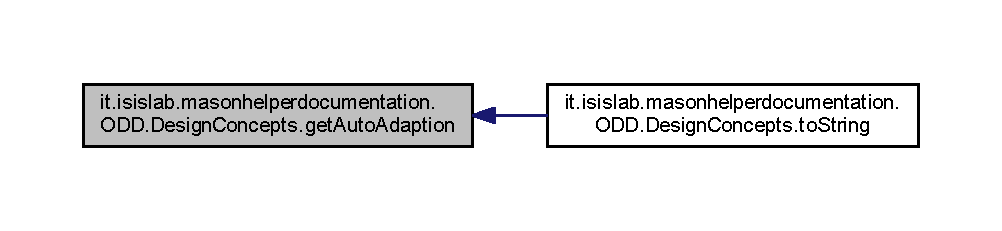
\includegraphics[width=350pt]{classit_1_1isislab_1_1masonhelperdocumentation_1_1_o_d_d_1_1_design_concepts_a93372a5bd13f71388909f6ca6ef7894f_icgraph}
\end{center}
\end{figure}


\hypertarget{classit_1_1isislab_1_1masonhelperdocumentation_1_1_o_d_d_1_1_design_concepts_adb4dd71450f8f1b5ad54a68b63a8662b}{\index{it\-::isislab\-::masonhelperdocumentation\-::\-O\-D\-D\-::\-Design\-Concepts@{it\-::isislab\-::masonhelperdocumentation\-::\-O\-D\-D\-::\-Design\-Concepts}!get\-Auto\-Basic\-Principles@{get\-Auto\-Basic\-Principles}}
\index{get\-Auto\-Basic\-Principles@{get\-Auto\-Basic\-Principles}!it::isislab::masonhelperdocumentation::ODD::DesignConcepts@{it\-::isislab\-::masonhelperdocumentation\-::\-O\-D\-D\-::\-Design\-Concepts}}
\subsubsection[{get\-Auto\-Basic\-Principles}]{\setlength{\rightskip}{0pt plus 5cm}String it.\-isislab.\-masonhelperdocumentation.\-O\-D\-D.\-Design\-Concepts.\-get\-Auto\-Basic\-Principles (
\begin{DoxyParamCaption}
{}
\end{DoxyParamCaption}
)}}\label{classit_1_1isislab_1_1masonhelperdocumentation_1_1_o_d_d_1_1_design_concepts_adb4dd71450f8f1b5ad54a68b63a8662b}

\begin{DoxyCode}
30                                            \{
31         \textcolor{keywordflow}{if} (\hyperlink{classit_1_1isislab_1_1masonhelperdocumentation_1_1_o_d_d_1_1_design_concepts_aa5a0af5b9002ffab0de5e9a219b39f8d}{autoBasicPrinciples} == null) \textcolor{keywordflow}{return} \textcolor{stringliteral}{""};
32         \textcolor{keywordflow}{return} \hyperlink{classit_1_1isislab_1_1masonhelperdocumentation_1_1_o_d_d_1_1_design_concepts_aa5a0af5b9002ffab0de5e9a219b39f8d}{autoBasicPrinciples};
33     \}
\end{DoxyCode}


Here is the caller graph for this function\-:
\nopagebreak
\begin{figure}[H]
\begin{center}
\leavevmode
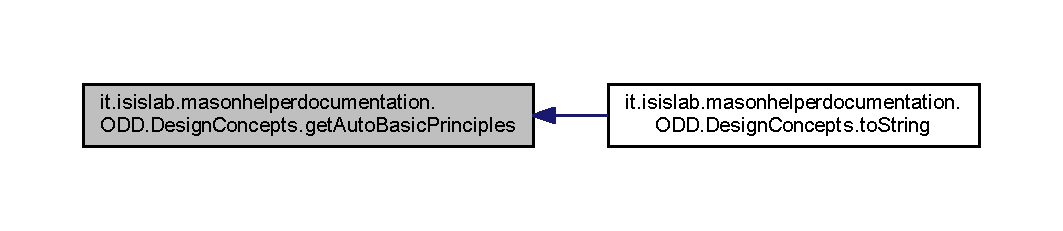
\includegraphics[width=350pt]{classit_1_1isislab_1_1masonhelperdocumentation_1_1_o_d_d_1_1_design_concepts_adb4dd71450f8f1b5ad54a68b63a8662b_icgraph}
\end{center}
\end{figure}


\hypertarget{classit_1_1isislab_1_1masonhelperdocumentation_1_1_o_d_d_1_1_design_concepts_a395311bdeaafed43497008c8cf540593}{\index{it\-::isislab\-::masonhelperdocumentation\-::\-O\-D\-D\-::\-Design\-Concepts@{it\-::isislab\-::masonhelperdocumentation\-::\-O\-D\-D\-::\-Design\-Concepts}!get\-Auto\-Collectives@{get\-Auto\-Collectives}}
\index{get\-Auto\-Collectives@{get\-Auto\-Collectives}!it::isislab::masonhelperdocumentation::ODD::DesignConcepts@{it\-::isislab\-::masonhelperdocumentation\-::\-O\-D\-D\-::\-Design\-Concepts}}
\subsubsection[{get\-Auto\-Collectives}]{\setlength{\rightskip}{0pt plus 5cm}String it.\-isislab.\-masonhelperdocumentation.\-O\-D\-D.\-Design\-Concepts.\-get\-Auto\-Collectives (
\begin{DoxyParamCaption}
{}
\end{DoxyParamCaption}
)}}\label{classit_1_1isislab_1_1masonhelperdocumentation_1_1_o_d_d_1_1_design_concepts_a395311bdeaafed43497008c8cf540593}

\begin{DoxyCode}
135                                        \{
136         \textcolor{keywordflow}{if} (\hyperlink{classit_1_1isislab_1_1masonhelperdocumentation_1_1_o_d_d_1_1_design_concepts_af913c6789584151bbfda5f4c49615560}{autoCollectives} == null) \textcolor{keywordflow}{return} \textcolor{stringliteral}{""};
137         \textcolor{keywordflow}{return} \hyperlink{classit_1_1isislab_1_1masonhelperdocumentation_1_1_o_d_d_1_1_design_concepts_af913c6789584151bbfda5f4c49615560}{autoCollectives};
138     \}
\end{DoxyCode}


Here is the caller graph for this function\-:
\nopagebreak
\begin{figure}[H]
\begin{center}
\leavevmode
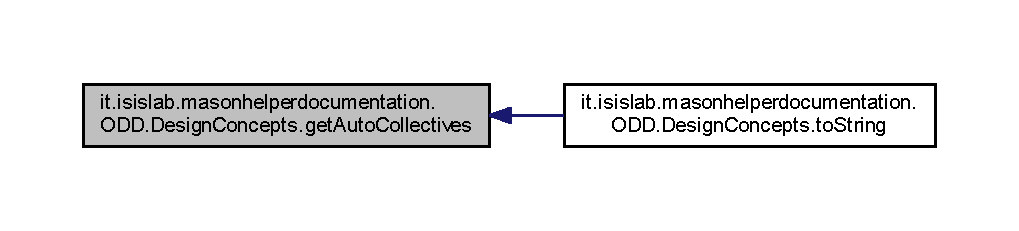
\includegraphics[width=350pt]{classit_1_1isislab_1_1masonhelperdocumentation_1_1_o_d_d_1_1_design_concepts_a395311bdeaafed43497008c8cf540593_icgraph}
\end{center}
\end{figure}


\hypertarget{classit_1_1isislab_1_1masonhelperdocumentation_1_1_o_d_d_1_1_design_concepts_acf594edfcc4e9666c82b2ff201902e3e}{\index{it\-::isislab\-::masonhelperdocumentation\-::\-O\-D\-D\-::\-Design\-Concepts@{it\-::isislab\-::masonhelperdocumentation\-::\-O\-D\-D\-::\-Design\-Concepts}!get\-Auto\-Emergence@{get\-Auto\-Emergence}}
\index{get\-Auto\-Emergence@{get\-Auto\-Emergence}!it::isislab::masonhelperdocumentation::ODD::DesignConcepts@{it\-::isislab\-::masonhelperdocumentation\-::\-O\-D\-D\-::\-Design\-Concepts}}
\subsubsection[{get\-Auto\-Emergence}]{\setlength{\rightskip}{0pt plus 5cm}String it.\-isislab.\-masonhelperdocumentation.\-O\-D\-D.\-Design\-Concepts.\-get\-Auto\-Emergence (
\begin{DoxyParamCaption}
{}
\end{DoxyParamCaption}
)}}\label{classit_1_1isislab_1_1masonhelperdocumentation_1_1_o_d_d_1_1_design_concepts_acf594edfcc4e9666c82b2ff201902e3e}

\begin{DoxyCode}
44                                      \{
45         \textcolor{keywordflow}{if} (\hyperlink{classit_1_1isislab_1_1masonhelperdocumentation_1_1_o_d_d_1_1_design_concepts_ab6e30191f9a5ecf4370bbbf5f9fe7eed}{autoEmergence} == null) \textcolor{keywordflow}{return} \textcolor{stringliteral}{""};
46         \textcolor{keywordflow}{return} \hyperlink{classit_1_1isislab_1_1masonhelperdocumentation_1_1_o_d_d_1_1_design_concepts_ab6e30191f9a5ecf4370bbbf5f9fe7eed}{autoEmergence};
47     \}
\end{DoxyCode}


Here is the caller graph for this function\-:
\nopagebreak
\begin{figure}[H]
\begin{center}
\leavevmode
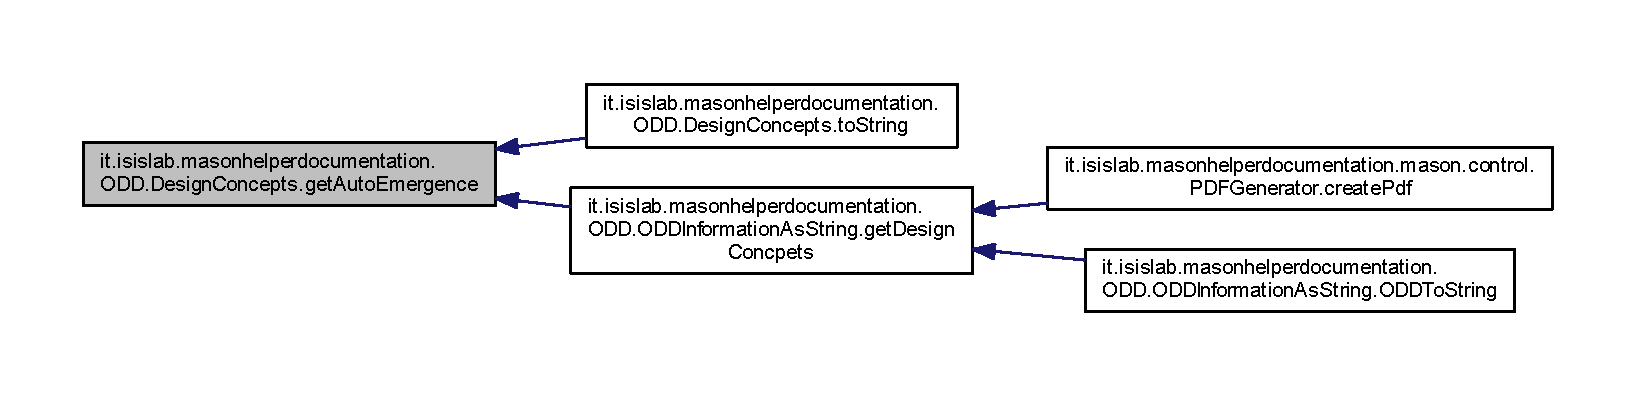
\includegraphics[width=350pt]{classit_1_1isislab_1_1masonhelperdocumentation_1_1_o_d_d_1_1_design_concepts_acf594edfcc4e9666c82b2ff201902e3e_icgraph}
\end{center}
\end{figure}


\hypertarget{classit_1_1isislab_1_1masonhelperdocumentation_1_1_o_d_d_1_1_design_concepts_a6183ce175da9ce0699a41ffad622572c}{\index{it\-::isislab\-::masonhelperdocumentation\-::\-O\-D\-D\-::\-Design\-Concepts@{it\-::isislab\-::masonhelperdocumentation\-::\-O\-D\-D\-::\-Design\-Concepts}!get\-Auto\-Interaction@{get\-Auto\-Interaction}}
\index{get\-Auto\-Interaction@{get\-Auto\-Interaction}!it::isislab::masonhelperdocumentation::ODD::DesignConcepts@{it\-::isislab\-::masonhelperdocumentation\-::\-O\-D\-D\-::\-Design\-Concepts}}
\subsubsection[{get\-Auto\-Interaction}]{\setlength{\rightskip}{0pt plus 5cm}String it.\-isislab.\-masonhelperdocumentation.\-O\-D\-D.\-Design\-Concepts.\-get\-Auto\-Interaction (
\begin{DoxyParamCaption}
{}
\end{DoxyParamCaption}
)}}\label{classit_1_1isislab_1_1masonhelperdocumentation_1_1_o_d_d_1_1_design_concepts_a6183ce175da9ce0699a41ffad622572c}

\begin{DoxyCode}
107                                        \{
108         \textcolor{keywordflow}{if} (\hyperlink{classit_1_1isislab_1_1masonhelperdocumentation_1_1_o_d_d_1_1_design_concepts_ac9990a36e827ad049dbe84779e7a4236}{autoInteraction} == null) \textcolor{keywordflow}{return} \textcolor{stringliteral}{""};
109         \textcolor{keywordflow}{return} \hyperlink{classit_1_1isislab_1_1masonhelperdocumentation_1_1_o_d_d_1_1_design_concepts_ac9990a36e827ad049dbe84779e7a4236}{autoInteraction};
110     \}
\end{DoxyCode}


Here is the caller graph for this function\-:
\nopagebreak
\begin{figure}[H]
\begin{center}
\leavevmode
\includegraphics[width=350pt]{classit_1_1isislab_1_1masonhelperdocumentation_1_1_o_d_d_1_1_design_concepts_a6183ce175da9ce0699a41ffad622572c_icgraph}
\end{center}
\end{figure}


\hypertarget{classit_1_1isislab_1_1masonhelperdocumentation_1_1_o_d_d_1_1_design_concepts_a682ad4da790d0c83948e7fa57e5c9bac}{\index{it\-::isislab\-::masonhelperdocumentation\-::\-O\-D\-D\-::\-Design\-Concepts@{it\-::isislab\-::masonhelperdocumentation\-::\-O\-D\-D\-::\-Design\-Concepts}!get\-Auto\-Learning@{get\-Auto\-Learning}}
\index{get\-Auto\-Learning@{get\-Auto\-Learning}!it::isislab::masonhelperdocumentation::ODD::DesignConcepts@{it\-::isislab\-::masonhelperdocumentation\-::\-O\-D\-D\-::\-Design\-Concepts}}
\subsubsection[{get\-Auto\-Learning}]{\setlength{\rightskip}{0pt plus 5cm}String it.\-isislab.\-masonhelperdocumentation.\-O\-D\-D.\-Design\-Concepts.\-get\-Auto\-Learning (
\begin{DoxyParamCaption}
{}
\end{DoxyParamCaption}
)}}\label{classit_1_1isislab_1_1masonhelperdocumentation_1_1_o_d_d_1_1_design_concepts_a682ad4da790d0c83948e7fa57e5c9bac}

\begin{DoxyCode}
86                                     \{
87         \textcolor{keywordflow}{if} (\hyperlink{classit_1_1isislab_1_1masonhelperdocumentation_1_1_o_d_d_1_1_design_concepts_ab8b75a5f651c2b0e6f03215951d31bff}{autoLearning} == null)   \textcolor{keywordflow}{return} \textcolor{stringliteral}{""};
88         \textcolor{keywordflow}{return} \hyperlink{classit_1_1isislab_1_1masonhelperdocumentation_1_1_o_d_d_1_1_design_concepts_ab8b75a5f651c2b0e6f03215951d31bff}{autoLearning};
89     \}
\end{DoxyCode}


Here is the caller graph for this function\-:
\nopagebreak
\begin{figure}[H]
\begin{center}
\leavevmode
\includegraphics[width=350pt]{classit_1_1isislab_1_1masonhelperdocumentation_1_1_o_d_d_1_1_design_concepts_a682ad4da790d0c83948e7fa57e5c9bac_icgraph}
\end{center}
\end{figure}


\hypertarget{classit_1_1isislab_1_1masonhelperdocumentation_1_1_o_d_d_1_1_design_concepts_adb483adb7985024c15c15e7ba3234f0e}{\index{it\-::isislab\-::masonhelperdocumentation\-::\-O\-D\-D\-::\-Design\-Concepts@{it\-::isislab\-::masonhelperdocumentation\-::\-O\-D\-D\-::\-Design\-Concepts}!get\-Auto\-Objectives@{get\-Auto\-Objectives}}
\index{get\-Auto\-Objectives@{get\-Auto\-Objectives}!it::isislab::masonhelperdocumentation::ODD::DesignConcepts@{it\-::isislab\-::masonhelperdocumentation\-::\-O\-D\-D\-::\-Design\-Concepts}}
\subsubsection[{get\-Auto\-Objectives}]{\setlength{\rightskip}{0pt plus 5cm}String it.\-isislab.\-masonhelperdocumentation.\-O\-D\-D.\-Design\-Concepts.\-get\-Auto\-Objectives (
\begin{DoxyParamCaption}
{}
\end{DoxyParamCaption}
)}}\label{classit_1_1isislab_1_1masonhelperdocumentation_1_1_o_d_d_1_1_design_concepts_adb483adb7985024c15c15e7ba3234f0e}

\begin{DoxyCode}
72                                       \{
73         \textcolor{keywordflow}{if} (\hyperlink{classit_1_1isislab_1_1masonhelperdocumentation_1_1_o_d_d_1_1_design_concepts_a9779cf8c34391d2ee20884fd2f01d831}{autoObjectives} == null)   \textcolor{keywordflow}{return} \textcolor{stringliteral}{""};
74         \textcolor{keywordflow}{return} \hyperlink{classit_1_1isislab_1_1masonhelperdocumentation_1_1_o_d_d_1_1_design_concepts_a9779cf8c34391d2ee20884fd2f01d831}{autoObjectives};
75     \}
\end{DoxyCode}


Here is the caller graph for this function\-:
\nopagebreak
\begin{figure}[H]
\begin{center}
\leavevmode
\includegraphics[width=350pt]{classit_1_1isislab_1_1masonhelperdocumentation_1_1_o_d_d_1_1_design_concepts_adb483adb7985024c15c15e7ba3234f0e_icgraph}
\end{center}
\end{figure}


\hypertarget{classit_1_1isislab_1_1masonhelperdocumentation_1_1_o_d_d_1_1_design_concepts_a8ad442e14c22ca8b344947c66cc24a9b}{\index{it\-::isislab\-::masonhelperdocumentation\-::\-O\-D\-D\-::\-Design\-Concepts@{it\-::isislab\-::masonhelperdocumentation\-::\-O\-D\-D\-::\-Design\-Concepts}!get\-Auto\-Observation@{get\-Auto\-Observation}}
\index{get\-Auto\-Observation@{get\-Auto\-Observation}!it::isislab::masonhelperdocumentation::ODD::DesignConcepts@{it\-::isislab\-::masonhelperdocumentation\-::\-O\-D\-D\-::\-Design\-Concepts}}
\subsubsection[{get\-Auto\-Observation}]{\setlength{\rightskip}{0pt plus 5cm}String it.\-isislab.\-masonhelperdocumentation.\-O\-D\-D.\-Design\-Concepts.\-get\-Auto\-Observation (
\begin{DoxyParamCaption}
{}
\end{DoxyParamCaption}
)}}\label{classit_1_1isislab_1_1masonhelperdocumentation_1_1_o_d_d_1_1_design_concepts_a8ad442e14c22ca8b344947c66cc24a9b}

\begin{DoxyCode}
149                                        \{
150         \textcolor{keywordflow}{if} (\hyperlink{classit_1_1isislab_1_1masonhelperdocumentation_1_1_o_d_d_1_1_design_concepts_a6f0867536a0f8ff0ff3d5870fccf0d1a}{autoObservation} == null) \textcolor{keywordflow}{return} \textcolor{stringliteral}{""};
151         \textcolor{keywordflow}{return} \hyperlink{classit_1_1isislab_1_1masonhelperdocumentation_1_1_o_d_d_1_1_design_concepts_a6f0867536a0f8ff0ff3d5870fccf0d1a}{autoObservation};
152     \}
\end{DoxyCode}


Here is the caller graph for this function\-:
\nopagebreak
\begin{figure}[H]
\begin{center}
\leavevmode
\includegraphics[width=350pt]{classit_1_1isislab_1_1masonhelperdocumentation_1_1_o_d_d_1_1_design_concepts_a8ad442e14c22ca8b344947c66cc24a9b_icgraph}
\end{center}
\end{figure}


\hypertarget{classit_1_1isislab_1_1masonhelperdocumentation_1_1_o_d_d_1_1_design_concepts_a266ecb29b4c1de8e7d59692b09463c59}{\index{it\-::isislab\-::masonhelperdocumentation\-::\-O\-D\-D\-::\-Design\-Concepts@{it\-::isislab\-::masonhelperdocumentation\-::\-O\-D\-D\-::\-Design\-Concepts}!get\-Auto\-Prediction@{get\-Auto\-Prediction}}
\index{get\-Auto\-Prediction@{get\-Auto\-Prediction}!it::isislab::masonhelperdocumentation::ODD::DesignConcepts@{it\-::isislab\-::masonhelperdocumentation\-::\-O\-D\-D\-::\-Design\-Concepts}}
\subsubsection[{get\-Auto\-Prediction}]{\setlength{\rightskip}{0pt plus 5cm}String it.\-isislab.\-masonhelperdocumentation.\-O\-D\-D.\-Design\-Concepts.\-get\-Auto\-Prediction (
\begin{DoxyParamCaption}
{}
\end{DoxyParamCaption}
)}}\label{classit_1_1isislab_1_1masonhelperdocumentation_1_1_o_d_d_1_1_design_concepts_a266ecb29b4c1de8e7d59692b09463c59}

\begin{DoxyCode}
163                                       \{
164         \textcolor{keywordflow}{if} (\hyperlink{classit_1_1isislab_1_1masonhelperdocumentation_1_1_o_d_d_1_1_design_concepts_a0fa295c94a753727d37958f540504870}{autoPrediction} == null)   \textcolor{keywordflow}{return} \textcolor{stringliteral}{""};
165         \textcolor{keywordflow}{return} \hyperlink{classit_1_1isislab_1_1masonhelperdocumentation_1_1_o_d_d_1_1_design_concepts_a0fa295c94a753727d37958f540504870}{autoPrediction};
166     \}
\end{DoxyCode}


Here is the caller graph for this function\-:
\nopagebreak
\begin{figure}[H]
\begin{center}
\leavevmode
\includegraphics[width=350pt]{classit_1_1isislab_1_1masonhelperdocumentation_1_1_o_d_d_1_1_design_concepts_a266ecb29b4c1de8e7d59692b09463c59_icgraph}
\end{center}
\end{figure}


\hypertarget{classit_1_1isislab_1_1masonhelperdocumentation_1_1_o_d_d_1_1_design_concepts_af20e006b60ffb46567d5cc72e78854de}{\index{it\-::isislab\-::masonhelperdocumentation\-::\-O\-D\-D\-::\-Design\-Concepts@{it\-::isislab\-::masonhelperdocumentation\-::\-O\-D\-D\-::\-Design\-Concepts}!get\-Auto\-Sensing@{get\-Auto\-Sensing}}
\index{get\-Auto\-Sensing@{get\-Auto\-Sensing}!it::isislab::masonhelperdocumentation::ODD::DesignConcepts@{it\-::isislab\-::masonhelperdocumentation\-::\-O\-D\-D\-::\-Design\-Concepts}}
\subsubsection[{get\-Auto\-Sensing}]{\setlength{\rightskip}{0pt plus 5cm}String it.\-isislab.\-masonhelperdocumentation.\-O\-D\-D.\-Design\-Concepts.\-get\-Auto\-Sensing (
\begin{DoxyParamCaption}
{}
\end{DoxyParamCaption}
)}}\label{classit_1_1isislab_1_1masonhelperdocumentation_1_1_o_d_d_1_1_design_concepts_af20e006b60ffb46567d5cc72e78854de}

\begin{DoxyCode}
93                                    \{
94         \textcolor{keywordflow}{if} (\hyperlink{classit_1_1isislab_1_1masonhelperdocumentation_1_1_o_d_d_1_1_design_concepts_a86a393d4a6748e83bcf6405a4afd5b28}{autoSensing} == null) \textcolor{keywordflow}{return} \textcolor{stringliteral}{""};
95         \textcolor{keywordflow}{return} \hyperlink{classit_1_1isislab_1_1masonhelperdocumentation_1_1_o_d_d_1_1_design_concepts_a86a393d4a6748e83bcf6405a4afd5b28}{autoSensing};
96     \}
\end{DoxyCode}


Here is the caller graph for this function\-:
\nopagebreak
\begin{figure}[H]
\begin{center}
\leavevmode
\includegraphics[width=350pt]{classit_1_1isislab_1_1masonhelperdocumentation_1_1_o_d_d_1_1_design_concepts_af20e006b60ffb46567d5cc72e78854de_icgraph}
\end{center}
\end{figure}


\hypertarget{classit_1_1isislab_1_1masonhelperdocumentation_1_1_o_d_d_1_1_design_concepts_a458e86699233a64459741e8f08961344}{\index{it\-::isislab\-::masonhelperdocumentation\-::\-O\-D\-D\-::\-Design\-Concepts@{it\-::isislab\-::masonhelperdocumentation\-::\-O\-D\-D\-::\-Design\-Concepts}!get\-Auto\-Stochasticity@{get\-Auto\-Stochasticity}}
\index{get\-Auto\-Stochasticity@{get\-Auto\-Stochasticity}!it::isislab::masonhelperdocumentation::ODD::DesignConcepts@{it\-::isislab\-::masonhelperdocumentation\-::\-O\-D\-D\-::\-Design\-Concepts}}
\subsubsection[{get\-Auto\-Stochasticity}]{\setlength{\rightskip}{0pt plus 5cm}String it.\-isislab.\-masonhelperdocumentation.\-O\-D\-D.\-Design\-Concepts.\-get\-Auto\-Stochasticity (
\begin{DoxyParamCaption}
{}
\end{DoxyParamCaption}
)}}\label{classit_1_1isislab_1_1masonhelperdocumentation_1_1_o_d_d_1_1_design_concepts_a458e86699233a64459741e8f08961344}

\begin{DoxyCode}
121                                          \{
122         \textcolor{keywordflow}{if} (\hyperlink{classit_1_1isislab_1_1masonhelperdocumentation_1_1_o_d_d_1_1_design_concepts_a9faf28491f90017f77a5024f73b66e23}{autoStochasticity} == null) \textcolor{keywordflow}{return} \textcolor{stringliteral}{""};
123         \textcolor{keywordflow}{return} \hyperlink{classit_1_1isislab_1_1masonhelperdocumentation_1_1_o_d_d_1_1_design_concepts_a9faf28491f90017f77a5024f73b66e23}{autoStochasticity};
124     \}
\end{DoxyCode}


Here is the caller graph for this function\-:
\nopagebreak
\begin{figure}[H]
\begin{center}
\leavevmode
\includegraphics[width=350pt]{classit_1_1isislab_1_1masonhelperdocumentation_1_1_o_d_d_1_1_design_concepts_a458e86699233a64459741e8f08961344_icgraph}
\end{center}
\end{figure}


\hypertarget{classit_1_1isislab_1_1masonhelperdocumentation_1_1_o_d_d_1_1_design_concepts_a605c0ea940f5be934c5e09e4ee7723d6}{\index{it\-::isislab\-::masonhelperdocumentation\-::\-O\-D\-D\-::\-Design\-Concepts@{it\-::isislab\-::masonhelperdocumentation\-::\-O\-D\-D\-::\-Design\-Concepts}!get\-User\-Adaption@{get\-User\-Adaption}}
\index{get\-User\-Adaption@{get\-User\-Adaption}!it::isislab::masonhelperdocumentation::ODD::DesignConcepts@{it\-::isislab\-::masonhelperdocumentation\-::\-O\-D\-D\-::\-Design\-Concepts}}
\subsubsection[{get\-User\-Adaption}]{\setlength{\rightskip}{0pt plus 5cm}String it.\-isislab.\-masonhelperdocumentation.\-O\-D\-D.\-Design\-Concepts.\-get\-User\-Adaption (
\begin{DoxyParamCaption}
{}
\end{DoxyParamCaption}
)}}\label{classit_1_1isislab_1_1masonhelperdocumentation_1_1_o_d_d_1_1_design_concepts_a605c0ea940f5be934c5e09e4ee7723d6}

\begin{DoxyCode}
65                                     \{
66         \textcolor{keywordflow}{if} (\hyperlink{classit_1_1isislab_1_1masonhelperdocumentation_1_1_o_d_d_1_1_design_concepts_a35c1ce4d16dce2293407c51606aa2643}{userAdaption} == null)   \textcolor{keywordflow}{return} \textcolor{stringliteral}{""};
67         \textcolor{keywordflow}{return} \hyperlink{classit_1_1isislab_1_1masonhelperdocumentation_1_1_o_d_d_1_1_design_concepts_a35c1ce4d16dce2293407c51606aa2643}{userAdaption};
68     \}
\end{DoxyCode}


Here is the caller graph for this function\-:
\nopagebreak
\begin{figure}[H]
\begin{center}
\leavevmode
\includegraphics[width=350pt]{classit_1_1isislab_1_1masonhelperdocumentation_1_1_o_d_d_1_1_design_concepts_a605c0ea940f5be934c5e09e4ee7723d6_icgraph}
\end{center}
\end{figure}


\hypertarget{classit_1_1isislab_1_1masonhelperdocumentation_1_1_o_d_d_1_1_design_concepts_ad4aa2370f8c035f66390e76db518ffcf}{\index{it\-::isislab\-::masonhelperdocumentation\-::\-O\-D\-D\-::\-Design\-Concepts@{it\-::isislab\-::masonhelperdocumentation\-::\-O\-D\-D\-::\-Design\-Concepts}!get\-User\-Basic\-Principles@{get\-User\-Basic\-Principles}}
\index{get\-User\-Basic\-Principles@{get\-User\-Basic\-Principles}!it::isislab::masonhelperdocumentation::ODD::DesignConcepts@{it\-::isislab\-::masonhelperdocumentation\-::\-O\-D\-D\-::\-Design\-Concepts}}
\subsubsection[{get\-User\-Basic\-Principles}]{\setlength{\rightskip}{0pt plus 5cm}String it.\-isislab.\-masonhelperdocumentation.\-O\-D\-D.\-Design\-Concepts.\-get\-User\-Basic\-Principles (
\begin{DoxyParamCaption}
{}
\end{DoxyParamCaption}
)}}\label{classit_1_1isislab_1_1masonhelperdocumentation_1_1_o_d_d_1_1_design_concepts_ad4aa2370f8c035f66390e76db518ffcf}

\begin{DoxyCode}
37                                            \{
38         \textcolor{keywordflow}{if} (\hyperlink{classit_1_1isislab_1_1masonhelperdocumentation_1_1_o_d_d_1_1_design_concepts_a8ef2c3be72c0336a64cdabbd91e82e07}{userBasicPrinciples} == null) \textcolor{keywordflow}{return} \textcolor{stringliteral}{""};
39         \textcolor{keywordflow}{return} \hyperlink{classit_1_1isislab_1_1masonhelperdocumentation_1_1_o_d_d_1_1_design_concepts_a8ef2c3be72c0336a64cdabbd91e82e07}{userBasicPrinciples};
40     \}
\end{DoxyCode}


Here is the caller graph for this function\-:
\nopagebreak
\begin{figure}[H]
\begin{center}
\leavevmode
\includegraphics[width=350pt]{classit_1_1isislab_1_1masonhelperdocumentation_1_1_o_d_d_1_1_design_concepts_ad4aa2370f8c035f66390e76db518ffcf_icgraph}
\end{center}
\end{figure}


\hypertarget{classit_1_1isislab_1_1masonhelperdocumentation_1_1_o_d_d_1_1_design_concepts_a32bbb6b2b23e83b77cf1e629711e440f}{\index{it\-::isislab\-::masonhelperdocumentation\-::\-O\-D\-D\-::\-Design\-Concepts@{it\-::isislab\-::masonhelperdocumentation\-::\-O\-D\-D\-::\-Design\-Concepts}!get\-User\-Collectives@{get\-User\-Collectives}}
\index{get\-User\-Collectives@{get\-User\-Collectives}!it::isislab::masonhelperdocumentation::ODD::DesignConcepts@{it\-::isislab\-::masonhelperdocumentation\-::\-O\-D\-D\-::\-Design\-Concepts}}
\subsubsection[{get\-User\-Collectives}]{\setlength{\rightskip}{0pt plus 5cm}String it.\-isislab.\-masonhelperdocumentation.\-O\-D\-D.\-Design\-Concepts.\-get\-User\-Collectives (
\begin{DoxyParamCaption}
{}
\end{DoxyParamCaption}
)}}\label{classit_1_1isislab_1_1masonhelperdocumentation_1_1_o_d_d_1_1_design_concepts_a32bbb6b2b23e83b77cf1e629711e440f}

\begin{DoxyCode}
142                                        \{
143         \textcolor{keywordflow}{if} (\hyperlink{classit_1_1isislab_1_1masonhelperdocumentation_1_1_o_d_d_1_1_design_concepts_aa05038a5453d5f2c2f825d3196111d44}{userCollectives} == null) \textcolor{keywordflow}{return} \textcolor{stringliteral}{""};
144         \textcolor{keywordflow}{return} \hyperlink{classit_1_1isislab_1_1masonhelperdocumentation_1_1_o_d_d_1_1_design_concepts_aa05038a5453d5f2c2f825d3196111d44}{userCollectives};
145     \}
\end{DoxyCode}


Here is the caller graph for this function\-:
\nopagebreak
\begin{figure}[H]
\begin{center}
\leavevmode
\includegraphics[width=350pt]{classit_1_1isislab_1_1masonhelperdocumentation_1_1_o_d_d_1_1_design_concepts_a32bbb6b2b23e83b77cf1e629711e440f_icgraph}
\end{center}
\end{figure}


\hypertarget{classit_1_1isislab_1_1masonhelperdocumentation_1_1_o_d_d_1_1_design_concepts_a47940c6e8a2b76b6058bf2eb1273101b}{\index{it\-::isislab\-::masonhelperdocumentation\-::\-O\-D\-D\-::\-Design\-Concepts@{it\-::isislab\-::masonhelperdocumentation\-::\-O\-D\-D\-::\-Design\-Concepts}!get\-User\-Emergence@{get\-User\-Emergence}}
\index{get\-User\-Emergence@{get\-User\-Emergence}!it::isislab::masonhelperdocumentation::ODD::DesignConcepts@{it\-::isislab\-::masonhelperdocumentation\-::\-O\-D\-D\-::\-Design\-Concepts}}
\subsubsection[{get\-User\-Emergence}]{\setlength{\rightskip}{0pt plus 5cm}String it.\-isislab.\-masonhelperdocumentation.\-O\-D\-D.\-Design\-Concepts.\-get\-User\-Emergence (
\begin{DoxyParamCaption}
{}
\end{DoxyParamCaption}
)}}\label{classit_1_1isislab_1_1masonhelperdocumentation_1_1_o_d_d_1_1_design_concepts_a47940c6e8a2b76b6058bf2eb1273101b}

\begin{DoxyCode}
51                                      \{
52         \textcolor{keywordflow}{if} (\hyperlink{classit_1_1isislab_1_1masonhelperdocumentation_1_1_o_d_d_1_1_design_concepts_a7a97f8bdb7fac0f86e4d070911eb07d0}{userEmergence} == null) \textcolor{keywordflow}{return} \textcolor{stringliteral}{""};
53         \textcolor{keywordflow}{return} \hyperlink{classit_1_1isislab_1_1masonhelperdocumentation_1_1_o_d_d_1_1_design_concepts_a7a97f8bdb7fac0f86e4d070911eb07d0}{userEmergence};
54     \}
\end{DoxyCode}


Here is the caller graph for this function\-:
\nopagebreak
\begin{figure}[H]
\begin{center}
\leavevmode
\includegraphics[width=350pt]{classit_1_1isislab_1_1masonhelperdocumentation_1_1_o_d_d_1_1_design_concepts_a47940c6e8a2b76b6058bf2eb1273101b_icgraph}
\end{center}
\end{figure}


\hypertarget{classit_1_1isislab_1_1masonhelperdocumentation_1_1_o_d_d_1_1_design_concepts_ae6d05ed191abb4725c7a5a7dc2d7449c}{\index{it\-::isislab\-::masonhelperdocumentation\-::\-O\-D\-D\-::\-Design\-Concepts@{it\-::isislab\-::masonhelperdocumentation\-::\-O\-D\-D\-::\-Design\-Concepts}!get\-User\-Interaction@{get\-User\-Interaction}}
\index{get\-User\-Interaction@{get\-User\-Interaction}!it::isislab::masonhelperdocumentation::ODD::DesignConcepts@{it\-::isislab\-::masonhelperdocumentation\-::\-O\-D\-D\-::\-Design\-Concepts}}
\subsubsection[{get\-User\-Interaction}]{\setlength{\rightskip}{0pt plus 5cm}String it.\-isislab.\-masonhelperdocumentation.\-O\-D\-D.\-Design\-Concepts.\-get\-User\-Interaction (
\begin{DoxyParamCaption}
{}
\end{DoxyParamCaption}
)}}\label{classit_1_1isislab_1_1masonhelperdocumentation_1_1_o_d_d_1_1_design_concepts_ae6d05ed191abb4725c7a5a7dc2d7449c}

\begin{DoxyCode}
114                                        \{
115         \textcolor{keywordflow}{if} (\hyperlink{classit_1_1isislab_1_1masonhelperdocumentation_1_1_o_d_d_1_1_design_concepts_ac597c8f95d3ce7cef3ef7f7b38b1da39}{userInteraction} == null) \textcolor{keywordflow}{return} \textcolor{stringliteral}{""};
116         \textcolor{keywordflow}{return} \hyperlink{classit_1_1isislab_1_1masonhelperdocumentation_1_1_o_d_d_1_1_design_concepts_ac597c8f95d3ce7cef3ef7f7b38b1da39}{userInteraction};
117     \}
\end{DoxyCode}


Here is the caller graph for this function\-:
\nopagebreak
\begin{figure}[H]
\begin{center}
\leavevmode
\includegraphics[width=350pt]{classit_1_1isislab_1_1masonhelperdocumentation_1_1_o_d_d_1_1_design_concepts_ae6d05ed191abb4725c7a5a7dc2d7449c_icgraph}
\end{center}
\end{figure}


\hypertarget{classit_1_1isislab_1_1masonhelperdocumentation_1_1_o_d_d_1_1_design_concepts_ab3d2b25545a723f677cf54548fc17ae2}{\index{it\-::isislab\-::masonhelperdocumentation\-::\-O\-D\-D\-::\-Design\-Concepts@{it\-::isislab\-::masonhelperdocumentation\-::\-O\-D\-D\-::\-Design\-Concepts}!get\-User\-Learning@{get\-User\-Learning}}
\index{get\-User\-Learning@{get\-User\-Learning}!it::isislab::masonhelperdocumentation::ODD::DesignConcepts@{it\-::isislab\-::masonhelperdocumentation\-::\-O\-D\-D\-::\-Design\-Concepts}}
\subsubsection[{get\-User\-Learning}]{\setlength{\rightskip}{0pt plus 5cm}String it.\-isislab.\-masonhelperdocumentation.\-O\-D\-D.\-Design\-Concepts.\-get\-User\-Learning (
\begin{DoxyParamCaption}
{}
\end{DoxyParamCaption}
)}}\label{classit_1_1isislab_1_1masonhelperdocumentation_1_1_o_d_d_1_1_design_concepts_ab3d2b25545a723f677cf54548fc17ae2}

\begin{DoxyCode}
180                                     \{
181         \textcolor{keywordflow}{if} (\hyperlink{classit_1_1isislab_1_1masonhelperdocumentation_1_1_o_d_d_1_1_design_concepts_a99d80f9502c09ab90d0d13ccb60be6c4}{userLearning} == null)   \textcolor{keywordflow}{return} \textcolor{stringliteral}{""};
182         \textcolor{keywordflow}{return} \hyperlink{classit_1_1isislab_1_1masonhelperdocumentation_1_1_o_d_d_1_1_design_concepts_a99d80f9502c09ab90d0d13ccb60be6c4}{userLearning};
183     \}   
\end{DoxyCode}


Here is the caller graph for this function\-:
\nopagebreak
\begin{figure}[H]
\begin{center}
\leavevmode
\includegraphics[width=350pt]{classit_1_1isislab_1_1masonhelperdocumentation_1_1_o_d_d_1_1_design_concepts_ab3d2b25545a723f677cf54548fc17ae2_icgraph}
\end{center}
\end{figure}


\hypertarget{classit_1_1isislab_1_1masonhelperdocumentation_1_1_o_d_d_1_1_design_concepts_afc17d14bd16ee6357780ca483158c877}{\index{it\-::isislab\-::masonhelperdocumentation\-::\-O\-D\-D\-::\-Design\-Concepts@{it\-::isislab\-::masonhelperdocumentation\-::\-O\-D\-D\-::\-Design\-Concepts}!get\-User\-Objectives@{get\-User\-Objectives}}
\index{get\-User\-Objectives@{get\-User\-Objectives}!it::isislab::masonhelperdocumentation::ODD::DesignConcepts@{it\-::isislab\-::masonhelperdocumentation\-::\-O\-D\-D\-::\-Design\-Concepts}}
\subsubsection[{get\-User\-Objectives}]{\setlength{\rightskip}{0pt plus 5cm}String it.\-isislab.\-masonhelperdocumentation.\-O\-D\-D.\-Design\-Concepts.\-get\-User\-Objectives (
\begin{DoxyParamCaption}
{}
\end{DoxyParamCaption}
)}}\label{classit_1_1isislab_1_1masonhelperdocumentation_1_1_o_d_d_1_1_design_concepts_afc17d14bd16ee6357780ca483158c877}

\begin{DoxyCode}
79                                       \{
80         \textcolor{keywordflow}{if} (\hyperlink{classit_1_1isislab_1_1masonhelperdocumentation_1_1_o_d_d_1_1_design_concepts_a274b0ccb901080375dfb9afeb548d52d}{userObjectives} == null)   \textcolor{keywordflow}{return} \textcolor{stringliteral}{""};
81         \textcolor{keywordflow}{return} \hyperlink{classit_1_1isislab_1_1masonhelperdocumentation_1_1_o_d_d_1_1_design_concepts_a274b0ccb901080375dfb9afeb548d52d}{userObjectives};
82     \}
\end{DoxyCode}


Here is the caller graph for this function\-:
\nopagebreak
\begin{figure}[H]
\begin{center}
\leavevmode
\includegraphics[width=350pt]{classit_1_1isislab_1_1masonhelperdocumentation_1_1_o_d_d_1_1_design_concepts_afc17d14bd16ee6357780ca483158c877_icgraph}
\end{center}
\end{figure}


\hypertarget{classit_1_1isislab_1_1masonhelperdocumentation_1_1_o_d_d_1_1_design_concepts_a27745de8ab804c2746ce0e90188f196d}{\index{it\-::isislab\-::masonhelperdocumentation\-::\-O\-D\-D\-::\-Design\-Concepts@{it\-::isislab\-::masonhelperdocumentation\-::\-O\-D\-D\-::\-Design\-Concepts}!get\-User\-Observation@{get\-User\-Observation}}
\index{get\-User\-Observation@{get\-User\-Observation}!it::isislab::masonhelperdocumentation::ODD::DesignConcepts@{it\-::isislab\-::masonhelperdocumentation\-::\-O\-D\-D\-::\-Design\-Concepts}}
\subsubsection[{get\-User\-Observation}]{\setlength{\rightskip}{0pt plus 5cm}String it.\-isislab.\-masonhelperdocumentation.\-O\-D\-D.\-Design\-Concepts.\-get\-User\-Observation (
\begin{DoxyParamCaption}
{}
\end{DoxyParamCaption}
)}}\label{classit_1_1isislab_1_1masonhelperdocumentation_1_1_o_d_d_1_1_design_concepts_a27745de8ab804c2746ce0e90188f196d}

\begin{DoxyCode}
156                                        \{
157         \textcolor{keywordflow}{if} (\hyperlink{classit_1_1isislab_1_1masonhelperdocumentation_1_1_o_d_d_1_1_design_concepts_a96c89d9c298a9c8782b83b7bb68041f9}{userObservation} == null) \textcolor{keywordflow}{return} \textcolor{stringliteral}{""};
158         \textcolor{keywordflow}{return} \hyperlink{classit_1_1isislab_1_1masonhelperdocumentation_1_1_o_d_d_1_1_design_concepts_a96c89d9c298a9c8782b83b7bb68041f9}{userObservation};
159     \}
\end{DoxyCode}


Here is the caller graph for this function\-:
\nopagebreak
\begin{figure}[H]
\begin{center}
\leavevmode
\includegraphics[width=350pt]{classit_1_1isislab_1_1masonhelperdocumentation_1_1_o_d_d_1_1_design_concepts_a27745de8ab804c2746ce0e90188f196d_icgraph}
\end{center}
\end{figure}


\hypertarget{classit_1_1isislab_1_1masonhelperdocumentation_1_1_o_d_d_1_1_design_concepts_a61fd3913e11fee85f390d52831ee63ea}{\index{it\-::isislab\-::masonhelperdocumentation\-::\-O\-D\-D\-::\-Design\-Concepts@{it\-::isislab\-::masonhelperdocumentation\-::\-O\-D\-D\-::\-Design\-Concepts}!get\-User\-Prediction@{get\-User\-Prediction}}
\index{get\-User\-Prediction@{get\-User\-Prediction}!it::isislab::masonhelperdocumentation::ODD::DesignConcepts@{it\-::isislab\-::masonhelperdocumentation\-::\-O\-D\-D\-::\-Design\-Concepts}}
\subsubsection[{get\-User\-Prediction}]{\setlength{\rightskip}{0pt plus 5cm}String it.\-isislab.\-masonhelperdocumentation.\-O\-D\-D.\-Design\-Concepts.\-get\-User\-Prediction (
\begin{DoxyParamCaption}
{}
\end{DoxyParamCaption}
)}}\label{classit_1_1isislab_1_1masonhelperdocumentation_1_1_o_d_d_1_1_design_concepts_a61fd3913e11fee85f390d52831ee63ea}

\begin{DoxyCode}
173                                       \{
174         \textcolor{keywordflow}{if} (\hyperlink{classit_1_1isislab_1_1masonhelperdocumentation_1_1_o_d_d_1_1_design_concepts_a753b8ac81cc11fb07e248cebadcc7494}{userPrediction} == null)   \textcolor{keywordflow}{return} \textcolor{stringliteral}{""};
175         \textcolor{keywordflow}{return} \hyperlink{classit_1_1isislab_1_1masonhelperdocumentation_1_1_o_d_d_1_1_design_concepts_a753b8ac81cc11fb07e248cebadcc7494}{userPrediction};
176     \}
\end{DoxyCode}


Here is the caller graph for this function\-:
\nopagebreak
\begin{figure}[H]
\begin{center}
\leavevmode
\includegraphics[width=350pt]{classit_1_1isislab_1_1masonhelperdocumentation_1_1_o_d_d_1_1_design_concepts_a61fd3913e11fee85f390d52831ee63ea_icgraph}
\end{center}
\end{figure}


\hypertarget{classit_1_1isislab_1_1masonhelperdocumentation_1_1_o_d_d_1_1_design_concepts_a5ef74e6cb5cd8e4fd0ac7299cf0aa2d9}{\index{it\-::isislab\-::masonhelperdocumentation\-::\-O\-D\-D\-::\-Design\-Concepts@{it\-::isislab\-::masonhelperdocumentation\-::\-O\-D\-D\-::\-Design\-Concepts}!get\-User\-Sensing@{get\-User\-Sensing}}
\index{get\-User\-Sensing@{get\-User\-Sensing}!it::isislab::masonhelperdocumentation::ODD::DesignConcepts@{it\-::isislab\-::masonhelperdocumentation\-::\-O\-D\-D\-::\-Design\-Concepts}}
\subsubsection[{get\-User\-Sensing}]{\setlength{\rightskip}{0pt plus 5cm}String it.\-isislab.\-masonhelperdocumentation.\-O\-D\-D.\-Design\-Concepts.\-get\-User\-Sensing (
\begin{DoxyParamCaption}
{}
\end{DoxyParamCaption}
)}}\label{classit_1_1isislab_1_1masonhelperdocumentation_1_1_o_d_d_1_1_design_concepts_a5ef74e6cb5cd8e4fd0ac7299cf0aa2d9}

\begin{DoxyCode}
100                                    \{
101         \textcolor{keywordflow}{if} (\hyperlink{classit_1_1isislab_1_1masonhelperdocumentation_1_1_o_d_d_1_1_design_concepts_a79cb2b2a618b459fff8bb1fc129ce3cf}{userSensing} == null) \textcolor{keywordflow}{return} \textcolor{stringliteral}{""};
102         \textcolor{keywordflow}{return} \hyperlink{classit_1_1isislab_1_1masonhelperdocumentation_1_1_o_d_d_1_1_design_concepts_a79cb2b2a618b459fff8bb1fc129ce3cf}{userSensing};
103     \}
\end{DoxyCode}


Here is the caller graph for this function\-:
\nopagebreak
\begin{figure}[H]
\begin{center}
\leavevmode
\includegraphics[width=350pt]{classit_1_1isislab_1_1masonhelperdocumentation_1_1_o_d_d_1_1_design_concepts_a5ef74e6cb5cd8e4fd0ac7299cf0aa2d9_icgraph}
\end{center}
\end{figure}


\hypertarget{classit_1_1isislab_1_1masonhelperdocumentation_1_1_o_d_d_1_1_design_concepts_ae4f7c2e729ebe125b5a9d8e92e1d2397}{\index{it\-::isislab\-::masonhelperdocumentation\-::\-O\-D\-D\-::\-Design\-Concepts@{it\-::isislab\-::masonhelperdocumentation\-::\-O\-D\-D\-::\-Design\-Concepts}!get\-User\-Stochasticity@{get\-User\-Stochasticity}}
\index{get\-User\-Stochasticity@{get\-User\-Stochasticity}!it::isislab::masonhelperdocumentation::ODD::DesignConcepts@{it\-::isislab\-::masonhelperdocumentation\-::\-O\-D\-D\-::\-Design\-Concepts}}
\subsubsection[{get\-User\-Stochasticity}]{\setlength{\rightskip}{0pt plus 5cm}String it.\-isislab.\-masonhelperdocumentation.\-O\-D\-D.\-Design\-Concepts.\-get\-User\-Stochasticity (
\begin{DoxyParamCaption}
{}
\end{DoxyParamCaption}
)}}\label{classit_1_1isislab_1_1masonhelperdocumentation_1_1_o_d_d_1_1_design_concepts_ae4f7c2e729ebe125b5a9d8e92e1d2397}

\begin{DoxyCode}
128                                          \{
129         \textcolor{keywordflow}{if} (\hyperlink{classit_1_1isislab_1_1masonhelperdocumentation_1_1_o_d_d_1_1_design_concepts_a927ab93d0fab6d30ff07bbd099a84163}{userStochasticity} == null) \textcolor{keywordflow}{return} \textcolor{stringliteral}{""};
130         \textcolor{keywordflow}{return} \hyperlink{classit_1_1isislab_1_1masonhelperdocumentation_1_1_o_d_d_1_1_design_concepts_a927ab93d0fab6d30ff07bbd099a84163}{userStochasticity};
131     \}
\end{DoxyCode}


Here is the caller graph for this function\-:
\nopagebreak
\begin{figure}[H]
\begin{center}
\leavevmode
\includegraphics[width=350pt]{classit_1_1isislab_1_1masonhelperdocumentation_1_1_o_d_d_1_1_design_concepts_ae4f7c2e729ebe125b5a9d8e92e1d2397_icgraph}
\end{center}
\end{figure}


\hypertarget{classit_1_1isislab_1_1masonhelperdocumentation_1_1_o_d_d_1_1_design_concepts_a7d179c91faf2b7a1cfdd4e1f45e7077b}{\index{it\-::isislab\-::masonhelperdocumentation\-::\-O\-D\-D\-::\-Design\-Concepts@{it\-::isislab\-::masonhelperdocumentation\-::\-O\-D\-D\-::\-Design\-Concepts}!set\-Auto\-Adaption@{set\-Auto\-Adaption}}
\index{set\-Auto\-Adaption@{set\-Auto\-Adaption}!it::isislab::masonhelperdocumentation::ODD::DesignConcepts@{it\-::isislab\-::masonhelperdocumentation\-::\-O\-D\-D\-::\-Design\-Concepts}}
\subsubsection[{set\-Auto\-Adaption}]{\setlength{\rightskip}{0pt plus 5cm}void it.\-isislab.\-masonhelperdocumentation.\-O\-D\-D.\-Design\-Concepts.\-set\-Auto\-Adaption (
\begin{DoxyParamCaption}
\item[{String}]{auto\-Adaption}
\end{DoxyParamCaption}
)}}\label{classit_1_1isislab_1_1masonhelperdocumentation_1_1_o_d_d_1_1_design_concepts_a7d179c91faf2b7a1cfdd4e1f45e7077b}

\begin{DoxyCode}
62                                                      \{
63         this.autoAdaption = \hyperlink{classit_1_1isislab_1_1masonhelperdocumentation_1_1_o_d_d_1_1_design_concepts_a22dcea289f1859841ee8ace538040550}{autoAdaption};
64     \}
\end{DoxyCode}
\hypertarget{classit_1_1isislab_1_1masonhelperdocumentation_1_1_o_d_d_1_1_design_concepts_a19c4d24937bd3d86da8b59308b47f3ba}{\index{it\-::isislab\-::masonhelperdocumentation\-::\-O\-D\-D\-::\-Design\-Concepts@{it\-::isislab\-::masonhelperdocumentation\-::\-O\-D\-D\-::\-Design\-Concepts}!set\-Auto\-Basic\-Principles@{set\-Auto\-Basic\-Principles}}
\index{set\-Auto\-Basic\-Principles@{set\-Auto\-Basic\-Principles}!it::isislab::masonhelperdocumentation::ODD::DesignConcepts@{it\-::isislab\-::masonhelperdocumentation\-::\-O\-D\-D\-::\-Design\-Concepts}}
\subsubsection[{set\-Auto\-Basic\-Principles}]{\setlength{\rightskip}{0pt plus 5cm}void it.\-isislab.\-masonhelperdocumentation.\-O\-D\-D.\-Design\-Concepts.\-set\-Auto\-Basic\-Principles (
\begin{DoxyParamCaption}
\item[{String}]{auto\-Basic\-Principles}
\end{DoxyParamCaption}
)}}\label{classit_1_1isislab_1_1masonhelperdocumentation_1_1_o_d_d_1_1_design_concepts_a19c4d24937bd3d86da8b59308b47f3ba}

\begin{DoxyCode}
34                                                                    \{
35         this.autoBasicPrinciples = \hyperlink{classit_1_1isislab_1_1masonhelperdocumentation_1_1_o_d_d_1_1_design_concepts_aa5a0af5b9002ffab0de5e9a219b39f8d}{autoBasicPrinciples};
36     \}
\end{DoxyCode}
\hypertarget{classit_1_1isislab_1_1masonhelperdocumentation_1_1_o_d_d_1_1_design_concepts_a84135c9c4ab80827345592f663650257}{\index{it\-::isislab\-::masonhelperdocumentation\-::\-O\-D\-D\-::\-Design\-Concepts@{it\-::isislab\-::masonhelperdocumentation\-::\-O\-D\-D\-::\-Design\-Concepts}!set\-Auto\-Collectives@{set\-Auto\-Collectives}}
\index{set\-Auto\-Collectives@{set\-Auto\-Collectives}!it::isislab::masonhelperdocumentation::ODD::DesignConcepts@{it\-::isislab\-::masonhelperdocumentation\-::\-O\-D\-D\-::\-Design\-Concepts}}
\subsubsection[{set\-Auto\-Collectives}]{\setlength{\rightskip}{0pt plus 5cm}void it.\-isislab.\-masonhelperdocumentation.\-O\-D\-D.\-Design\-Concepts.\-set\-Auto\-Collectives (
\begin{DoxyParamCaption}
\item[{String}]{auto\-Collectives}
\end{DoxyParamCaption}
)}}\label{classit_1_1isislab_1_1masonhelperdocumentation_1_1_o_d_d_1_1_design_concepts_a84135c9c4ab80827345592f663650257}

\begin{DoxyCode}
139                                                            \{
140         this.autoCollectives = \hyperlink{classit_1_1isislab_1_1masonhelperdocumentation_1_1_o_d_d_1_1_design_concepts_af913c6789584151bbfda5f4c49615560}{autoCollectives};
141     \}
\end{DoxyCode}
\hypertarget{classit_1_1isislab_1_1masonhelperdocumentation_1_1_o_d_d_1_1_design_concepts_acaf605cd934578b681e95e0a31fb715d}{\index{it\-::isislab\-::masonhelperdocumentation\-::\-O\-D\-D\-::\-Design\-Concepts@{it\-::isislab\-::masonhelperdocumentation\-::\-O\-D\-D\-::\-Design\-Concepts}!set\-Auto\-Emergence@{set\-Auto\-Emergence}}
\index{set\-Auto\-Emergence@{set\-Auto\-Emergence}!it::isislab::masonhelperdocumentation::ODD::DesignConcepts@{it\-::isislab\-::masonhelperdocumentation\-::\-O\-D\-D\-::\-Design\-Concepts}}
\subsubsection[{set\-Auto\-Emergence}]{\setlength{\rightskip}{0pt plus 5cm}void it.\-isislab.\-masonhelperdocumentation.\-O\-D\-D.\-Design\-Concepts.\-set\-Auto\-Emergence (
\begin{DoxyParamCaption}
\item[{String}]{auto\-Emergence}
\end{DoxyParamCaption}
)}}\label{classit_1_1isislab_1_1masonhelperdocumentation_1_1_o_d_d_1_1_design_concepts_acaf605cd934578b681e95e0a31fb715d}

\begin{DoxyCode}
48                                                        \{
49         this.autoEmergence = \hyperlink{classit_1_1isislab_1_1masonhelperdocumentation_1_1_o_d_d_1_1_design_concepts_ab6e30191f9a5ecf4370bbbf5f9fe7eed}{autoEmergence};
50     \}
\end{DoxyCode}
\hypertarget{classit_1_1isislab_1_1masonhelperdocumentation_1_1_o_d_d_1_1_design_concepts_a302c088646a48acd5470d178cf370265}{\index{it\-::isislab\-::masonhelperdocumentation\-::\-O\-D\-D\-::\-Design\-Concepts@{it\-::isislab\-::masonhelperdocumentation\-::\-O\-D\-D\-::\-Design\-Concepts}!set\-Auto\-Interaction@{set\-Auto\-Interaction}}
\index{set\-Auto\-Interaction@{set\-Auto\-Interaction}!it::isislab::masonhelperdocumentation::ODD::DesignConcepts@{it\-::isislab\-::masonhelperdocumentation\-::\-O\-D\-D\-::\-Design\-Concepts}}
\subsubsection[{set\-Auto\-Interaction}]{\setlength{\rightskip}{0pt plus 5cm}void it.\-isislab.\-masonhelperdocumentation.\-O\-D\-D.\-Design\-Concepts.\-set\-Auto\-Interaction (
\begin{DoxyParamCaption}
\item[{String}]{auto\-Interaction}
\end{DoxyParamCaption}
)}}\label{classit_1_1isislab_1_1masonhelperdocumentation_1_1_o_d_d_1_1_design_concepts_a302c088646a48acd5470d178cf370265}

\begin{DoxyCode}
111                                                            \{
112         this.autoInteraction = \hyperlink{classit_1_1isislab_1_1masonhelperdocumentation_1_1_o_d_d_1_1_design_concepts_ac9990a36e827ad049dbe84779e7a4236}{autoInteraction};
113     \}
\end{DoxyCode}
\hypertarget{classit_1_1isislab_1_1masonhelperdocumentation_1_1_o_d_d_1_1_design_concepts_a3d5ae0f19bca8e05bf9c1d46ba1f2483}{\index{it\-::isislab\-::masonhelperdocumentation\-::\-O\-D\-D\-::\-Design\-Concepts@{it\-::isislab\-::masonhelperdocumentation\-::\-O\-D\-D\-::\-Design\-Concepts}!set\-Auto\-Learning@{set\-Auto\-Learning}}
\index{set\-Auto\-Learning@{set\-Auto\-Learning}!it::isislab::masonhelperdocumentation::ODD::DesignConcepts@{it\-::isislab\-::masonhelperdocumentation\-::\-O\-D\-D\-::\-Design\-Concepts}}
\subsubsection[{set\-Auto\-Learning}]{\setlength{\rightskip}{0pt plus 5cm}void it.\-isislab.\-masonhelperdocumentation.\-O\-D\-D.\-Design\-Concepts.\-set\-Auto\-Learning (
\begin{DoxyParamCaption}
\item[{String}]{auto\-Learning}
\end{DoxyParamCaption}
)}}\label{classit_1_1isislab_1_1masonhelperdocumentation_1_1_o_d_d_1_1_design_concepts_a3d5ae0f19bca8e05bf9c1d46ba1f2483}

\begin{DoxyCode}
90                                                      \{
91         this.autoLearning = \hyperlink{classit_1_1isislab_1_1masonhelperdocumentation_1_1_o_d_d_1_1_design_concepts_ab8b75a5f651c2b0e6f03215951d31bff}{autoLearning};
92     \}
\end{DoxyCode}
\hypertarget{classit_1_1isislab_1_1masonhelperdocumentation_1_1_o_d_d_1_1_design_concepts_a55ea5d7ff35fd90004b7688fb810c814}{\index{it\-::isislab\-::masonhelperdocumentation\-::\-O\-D\-D\-::\-Design\-Concepts@{it\-::isislab\-::masonhelperdocumentation\-::\-O\-D\-D\-::\-Design\-Concepts}!set\-Auto\-Objectives@{set\-Auto\-Objectives}}
\index{set\-Auto\-Objectives@{set\-Auto\-Objectives}!it::isislab::masonhelperdocumentation::ODD::DesignConcepts@{it\-::isislab\-::masonhelperdocumentation\-::\-O\-D\-D\-::\-Design\-Concepts}}
\subsubsection[{set\-Auto\-Objectives}]{\setlength{\rightskip}{0pt plus 5cm}void it.\-isislab.\-masonhelperdocumentation.\-O\-D\-D.\-Design\-Concepts.\-set\-Auto\-Objectives (
\begin{DoxyParamCaption}
\item[{String}]{auto\-Objectives}
\end{DoxyParamCaption}
)}}\label{classit_1_1isislab_1_1masonhelperdocumentation_1_1_o_d_d_1_1_design_concepts_a55ea5d7ff35fd90004b7688fb810c814}

\begin{DoxyCode}
76                                                          \{
77         this.autoObjectives = \hyperlink{classit_1_1isislab_1_1masonhelperdocumentation_1_1_o_d_d_1_1_design_concepts_a9779cf8c34391d2ee20884fd2f01d831}{autoObjectives};
78     \}
\end{DoxyCode}
\hypertarget{classit_1_1isislab_1_1masonhelperdocumentation_1_1_o_d_d_1_1_design_concepts_a5f683fba4d025ee2fc04b1a547293ada}{\index{it\-::isislab\-::masonhelperdocumentation\-::\-O\-D\-D\-::\-Design\-Concepts@{it\-::isislab\-::masonhelperdocumentation\-::\-O\-D\-D\-::\-Design\-Concepts}!set\-Auto\-Observation@{set\-Auto\-Observation}}
\index{set\-Auto\-Observation@{set\-Auto\-Observation}!it::isislab::masonhelperdocumentation::ODD::DesignConcepts@{it\-::isislab\-::masonhelperdocumentation\-::\-O\-D\-D\-::\-Design\-Concepts}}
\subsubsection[{set\-Auto\-Observation}]{\setlength{\rightskip}{0pt plus 5cm}void it.\-isislab.\-masonhelperdocumentation.\-O\-D\-D.\-Design\-Concepts.\-set\-Auto\-Observation (
\begin{DoxyParamCaption}
\item[{String}]{auto\-Observation}
\end{DoxyParamCaption}
)}}\label{classit_1_1isislab_1_1masonhelperdocumentation_1_1_o_d_d_1_1_design_concepts_a5f683fba4d025ee2fc04b1a547293ada}

\begin{DoxyCode}
153                                                            \{
154         this.autoObservation = \hyperlink{classit_1_1isislab_1_1masonhelperdocumentation_1_1_o_d_d_1_1_design_concepts_a6f0867536a0f8ff0ff3d5870fccf0d1a}{autoObservation};
155     \}
\end{DoxyCode}
\hypertarget{classit_1_1isislab_1_1masonhelperdocumentation_1_1_o_d_d_1_1_design_concepts_adffe83b119875f2188374e6566d5cc30}{\index{it\-::isislab\-::masonhelperdocumentation\-::\-O\-D\-D\-::\-Design\-Concepts@{it\-::isislab\-::masonhelperdocumentation\-::\-O\-D\-D\-::\-Design\-Concepts}!set\-Auto\-Prediction@{set\-Auto\-Prediction}}
\index{set\-Auto\-Prediction@{set\-Auto\-Prediction}!it::isislab::masonhelperdocumentation::ODD::DesignConcepts@{it\-::isislab\-::masonhelperdocumentation\-::\-O\-D\-D\-::\-Design\-Concepts}}
\subsubsection[{set\-Auto\-Prediction}]{\setlength{\rightskip}{0pt plus 5cm}void it.\-isislab.\-masonhelperdocumentation.\-O\-D\-D.\-Design\-Concepts.\-set\-Auto\-Prediction (
\begin{DoxyParamCaption}
\item[{String}]{auto\-Prediction}
\end{DoxyParamCaption}
)}}\label{classit_1_1isislab_1_1masonhelperdocumentation_1_1_o_d_d_1_1_design_concepts_adffe83b119875f2188374e6566d5cc30}

\begin{DoxyCode}
167                                                          \{
168         this.autoPrediction = \hyperlink{classit_1_1isislab_1_1masonhelperdocumentation_1_1_o_d_d_1_1_design_concepts_a0fa295c94a753727d37958f540504870}{autoPrediction};
169     \}
\end{DoxyCode}
\hypertarget{classit_1_1isislab_1_1masonhelperdocumentation_1_1_o_d_d_1_1_design_concepts_a57228ab46a179a508590d9129043aa5b}{\index{it\-::isislab\-::masonhelperdocumentation\-::\-O\-D\-D\-::\-Design\-Concepts@{it\-::isislab\-::masonhelperdocumentation\-::\-O\-D\-D\-::\-Design\-Concepts}!set\-Auto\-Sensing@{set\-Auto\-Sensing}}
\index{set\-Auto\-Sensing@{set\-Auto\-Sensing}!it::isislab::masonhelperdocumentation::ODD::DesignConcepts@{it\-::isislab\-::masonhelperdocumentation\-::\-O\-D\-D\-::\-Design\-Concepts}}
\subsubsection[{set\-Auto\-Sensing}]{\setlength{\rightskip}{0pt plus 5cm}void it.\-isislab.\-masonhelperdocumentation.\-O\-D\-D.\-Design\-Concepts.\-set\-Auto\-Sensing (
\begin{DoxyParamCaption}
\item[{String}]{auto\-Sensing}
\end{DoxyParamCaption}
)}}\label{classit_1_1isislab_1_1masonhelperdocumentation_1_1_o_d_d_1_1_design_concepts_a57228ab46a179a508590d9129043aa5b}

\begin{DoxyCode}
97                                                    \{
98         this.autoSensing = \hyperlink{classit_1_1isislab_1_1masonhelperdocumentation_1_1_o_d_d_1_1_design_concepts_a86a393d4a6748e83bcf6405a4afd5b28}{autoSensing};
99     \}
\end{DoxyCode}
\hypertarget{classit_1_1isislab_1_1masonhelperdocumentation_1_1_o_d_d_1_1_design_concepts_a156529f8f025bb4c7d5bf33ef77da9da}{\index{it\-::isislab\-::masonhelperdocumentation\-::\-O\-D\-D\-::\-Design\-Concepts@{it\-::isislab\-::masonhelperdocumentation\-::\-O\-D\-D\-::\-Design\-Concepts}!set\-Auto\-Stochasticity@{set\-Auto\-Stochasticity}}
\index{set\-Auto\-Stochasticity@{set\-Auto\-Stochasticity}!it::isislab::masonhelperdocumentation::ODD::DesignConcepts@{it\-::isislab\-::masonhelperdocumentation\-::\-O\-D\-D\-::\-Design\-Concepts}}
\subsubsection[{set\-Auto\-Stochasticity}]{\setlength{\rightskip}{0pt plus 5cm}void it.\-isislab.\-masonhelperdocumentation.\-O\-D\-D.\-Design\-Concepts.\-set\-Auto\-Stochasticity (
\begin{DoxyParamCaption}
\item[{String}]{auto\-Stochasticity}
\end{DoxyParamCaption}
)}}\label{classit_1_1isislab_1_1masonhelperdocumentation_1_1_o_d_d_1_1_design_concepts_a156529f8f025bb4c7d5bf33ef77da9da}

\begin{DoxyCode}
125                                                                \{
126         this.autoStochasticity = \hyperlink{classit_1_1isislab_1_1masonhelperdocumentation_1_1_o_d_d_1_1_design_concepts_a9faf28491f90017f77a5024f73b66e23}{autoStochasticity};
127     \}
\end{DoxyCode}
\hypertarget{classit_1_1isislab_1_1masonhelperdocumentation_1_1_o_d_d_1_1_design_concepts_abf0895098a6a5a21366bc02c6e2c0f28}{\index{it\-::isislab\-::masonhelperdocumentation\-::\-O\-D\-D\-::\-Design\-Concepts@{it\-::isislab\-::masonhelperdocumentation\-::\-O\-D\-D\-::\-Design\-Concepts}!set\-User\-Adaption@{set\-User\-Adaption}}
\index{set\-User\-Adaption@{set\-User\-Adaption}!it::isislab::masonhelperdocumentation::ODD::DesignConcepts@{it\-::isislab\-::masonhelperdocumentation\-::\-O\-D\-D\-::\-Design\-Concepts}}
\subsubsection[{set\-User\-Adaption}]{\setlength{\rightskip}{0pt plus 5cm}void it.\-isislab.\-masonhelperdocumentation.\-O\-D\-D.\-Design\-Concepts.\-set\-User\-Adaption (
\begin{DoxyParamCaption}
\item[{String}]{user\-Adaption}
\end{DoxyParamCaption}
)}}\label{classit_1_1isislab_1_1masonhelperdocumentation_1_1_o_d_d_1_1_design_concepts_abf0895098a6a5a21366bc02c6e2c0f28}

\begin{DoxyCode}
69                                                      \{
70         this.userAdaption = \hyperlink{classit_1_1isislab_1_1masonhelperdocumentation_1_1_o_d_d_1_1_design_concepts_a35c1ce4d16dce2293407c51606aa2643}{userAdaption};
71     \}
\end{DoxyCode}
\hypertarget{classit_1_1isislab_1_1masonhelperdocumentation_1_1_o_d_d_1_1_design_concepts_ac73d2fb492849360c3c4f8dfb99f263a}{\index{it\-::isislab\-::masonhelperdocumentation\-::\-O\-D\-D\-::\-Design\-Concepts@{it\-::isislab\-::masonhelperdocumentation\-::\-O\-D\-D\-::\-Design\-Concepts}!set\-User\-Basic\-Principles@{set\-User\-Basic\-Principles}}
\index{set\-User\-Basic\-Principles@{set\-User\-Basic\-Principles}!it::isislab::masonhelperdocumentation::ODD::DesignConcepts@{it\-::isislab\-::masonhelperdocumentation\-::\-O\-D\-D\-::\-Design\-Concepts}}
\subsubsection[{set\-User\-Basic\-Principles}]{\setlength{\rightskip}{0pt plus 5cm}void it.\-isislab.\-masonhelperdocumentation.\-O\-D\-D.\-Design\-Concepts.\-set\-User\-Basic\-Principles (
\begin{DoxyParamCaption}
\item[{String}]{user\-Basic\-Principles}
\end{DoxyParamCaption}
)}}\label{classit_1_1isislab_1_1masonhelperdocumentation_1_1_o_d_d_1_1_design_concepts_ac73d2fb492849360c3c4f8dfb99f263a}

\begin{DoxyCode}
41                                                                    \{
42         this.userBasicPrinciples = \hyperlink{classit_1_1isislab_1_1masonhelperdocumentation_1_1_o_d_d_1_1_design_concepts_a8ef2c3be72c0336a64cdabbd91e82e07}{userBasicPrinciples};
43     \}
\end{DoxyCode}
\hypertarget{classit_1_1isislab_1_1masonhelperdocumentation_1_1_o_d_d_1_1_design_concepts_ace197154f72f101f69750cf771cc2154}{\index{it\-::isislab\-::masonhelperdocumentation\-::\-O\-D\-D\-::\-Design\-Concepts@{it\-::isislab\-::masonhelperdocumentation\-::\-O\-D\-D\-::\-Design\-Concepts}!set\-User\-Collectives@{set\-User\-Collectives}}
\index{set\-User\-Collectives@{set\-User\-Collectives}!it::isislab::masonhelperdocumentation::ODD::DesignConcepts@{it\-::isislab\-::masonhelperdocumentation\-::\-O\-D\-D\-::\-Design\-Concepts}}
\subsubsection[{set\-User\-Collectives}]{\setlength{\rightskip}{0pt plus 5cm}void it.\-isislab.\-masonhelperdocumentation.\-O\-D\-D.\-Design\-Concepts.\-set\-User\-Collectives (
\begin{DoxyParamCaption}
\item[{String}]{user\-Collectives}
\end{DoxyParamCaption}
)}}\label{classit_1_1isislab_1_1masonhelperdocumentation_1_1_o_d_d_1_1_design_concepts_ace197154f72f101f69750cf771cc2154}

\begin{DoxyCode}
146                                                            \{
147         this.userCollectives = \hyperlink{classit_1_1isislab_1_1masonhelperdocumentation_1_1_o_d_d_1_1_design_concepts_aa05038a5453d5f2c2f825d3196111d44}{userCollectives};
148     \}
\end{DoxyCode}
\hypertarget{classit_1_1isislab_1_1masonhelperdocumentation_1_1_o_d_d_1_1_design_concepts_a3d37971fb6c38bed0cb73d342165de96}{\index{it\-::isislab\-::masonhelperdocumentation\-::\-O\-D\-D\-::\-Design\-Concepts@{it\-::isislab\-::masonhelperdocumentation\-::\-O\-D\-D\-::\-Design\-Concepts}!set\-User\-Emergence@{set\-User\-Emergence}}
\index{set\-User\-Emergence@{set\-User\-Emergence}!it::isislab::masonhelperdocumentation::ODD::DesignConcepts@{it\-::isislab\-::masonhelperdocumentation\-::\-O\-D\-D\-::\-Design\-Concepts}}
\subsubsection[{set\-User\-Emergence}]{\setlength{\rightskip}{0pt plus 5cm}void it.\-isislab.\-masonhelperdocumentation.\-O\-D\-D.\-Design\-Concepts.\-set\-User\-Emergence (
\begin{DoxyParamCaption}
\item[{String}]{user\-Emergence}
\end{DoxyParamCaption}
)}}\label{classit_1_1isislab_1_1masonhelperdocumentation_1_1_o_d_d_1_1_design_concepts_a3d37971fb6c38bed0cb73d342165de96}

\begin{DoxyCode}
55                                                        \{
56         this.userEmergence = \hyperlink{classit_1_1isislab_1_1masonhelperdocumentation_1_1_o_d_d_1_1_design_concepts_a7a97f8bdb7fac0f86e4d070911eb07d0}{userEmergence};
57     \}
\end{DoxyCode}
\hypertarget{classit_1_1isislab_1_1masonhelperdocumentation_1_1_o_d_d_1_1_design_concepts_abcda82a77ad002de148d9be3fbda833a}{\index{it\-::isislab\-::masonhelperdocumentation\-::\-O\-D\-D\-::\-Design\-Concepts@{it\-::isislab\-::masonhelperdocumentation\-::\-O\-D\-D\-::\-Design\-Concepts}!set\-User\-Interaction@{set\-User\-Interaction}}
\index{set\-User\-Interaction@{set\-User\-Interaction}!it::isislab::masonhelperdocumentation::ODD::DesignConcepts@{it\-::isislab\-::masonhelperdocumentation\-::\-O\-D\-D\-::\-Design\-Concepts}}
\subsubsection[{set\-User\-Interaction}]{\setlength{\rightskip}{0pt plus 5cm}void it.\-isislab.\-masonhelperdocumentation.\-O\-D\-D.\-Design\-Concepts.\-set\-User\-Interaction (
\begin{DoxyParamCaption}
\item[{String}]{user\-Interaction}
\end{DoxyParamCaption}
)}}\label{classit_1_1isislab_1_1masonhelperdocumentation_1_1_o_d_d_1_1_design_concepts_abcda82a77ad002de148d9be3fbda833a}

\begin{DoxyCode}
118                                                            \{
119         this.userInteraction = \hyperlink{classit_1_1isislab_1_1masonhelperdocumentation_1_1_o_d_d_1_1_design_concepts_ac597c8f95d3ce7cef3ef7f7b38b1da39}{userInteraction};
120     \}
\end{DoxyCode}
\hypertarget{classit_1_1isislab_1_1masonhelperdocumentation_1_1_o_d_d_1_1_design_concepts_a38cfa461985c50771001b5449ea303c9}{\index{it\-::isislab\-::masonhelperdocumentation\-::\-O\-D\-D\-::\-Design\-Concepts@{it\-::isislab\-::masonhelperdocumentation\-::\-O\-D\-D\-::\-Design\-Concepts}!set\-User\-Learning@{set\-User\-Learning}}
\index{set\-User\-Learning@{set\-User\-Learning}!it::isislab::masonhelperdocumentation::ODD::DesignConcepts@{it\-::isislab\-::masonhelperdocumentation\-::\-O\-D\-D\-::\-Design\-Concepts}}
\subsubsection[{set\-User\-Learning}]{\setlength{\rightskip}{0pt plus 5cm}void it.\-isislab.\-masonhelperdocumentation.\-O\-D\-D.\-Design\-Concepts.\-set\-User\-Learning (
\begin{DoxyParamCaption}
\item[{String}]{user\-Learning}
\end{DoxyParamCaption}
)}}\label{classit_1_1isislab_1_1masonhelperdocumentation_1_1_o_d_d_1_1_design_concepts_a38cfa461985c50771001b5449ea303c9}

\begin{DoxyCode}
170                                                      \{
171         this.userLearning = \hyperlink{classit_1_1isislab_1_1masonhelperdocumentation_1_1_o_d_d_1_1_design_concepts_a99d80f9502c09ab90d0d13ccb60be6c4}{userLearning};
172     \}
\end{DoxyCode}
\hypertarget{classit_1_1isislab_1_1masonhelperdocumentation_1_1_o_d_d_1_1_design_concepts_ae4661a5bd3f3d8f5c576ef8d7578844d}{\index{it\-::isislab\-::masonhelperdocumentation\-::\-O\-D\-D\-::\-Design\-Concepts@{it\-::isislab\-::masonhelperdocumentation\-::\-O\-D\-D\-::\-Design\-Concepts}!set\-User\-Objectives@{set\-User\-Objectives}}
\index{set\-User\-Objectives@{set\-User\-Objectives}!it::isislab::masonhelperdocumentation::ODD::DesignConcepts@{it\-::isislab\-::masonhelperdocumentation\-::\-O\-D\-D\-::\-Design\-Concepts}}
\subsubsection[{set\-User\-Objectives}]{\setlength{\rightskip}{0pt plus 5cm}void it.\-isislab.\-masonhelperdocumentation.\-O\-D\-D.\-Design\-Concepts.\-set\-User\-Objectives (
\begin{DoxyParamCaption}
\item[{String}]{user\-Objectives}
\end{DoxyParamCaption}
)}}\label{classit_1_1isislab_1_1masonhelperdocumentation_1_1_o_d_d_1_1_design_concepts_ae4661a5bd3f3d8f5c576ef8d7578844d}

\begin{DoxyCode}
83                                                          \{
84         this.userObjectives = \hyperlink{classit_1_1isislab_1_1masonhelperdocumentation_1_1_o_d_d_1_1_design_concepts_a274b0ccb901080375dfb9afeb548d52d}{userObjectives};
85     \}
\end{DoxyCode}
\hypertarget{classit_1_1isislab_1_1masonhelperdocumentation_1_1_o_d_d_1_1_design_concepts_aee77661b7e66d50061dde8494c3b22ae}{\index{it\-::isislab\-::masonhelperdocumentation\-::\-O\-D\-D\-::\-Design\-Concepts@{it\-::isislab\-::masonhelperdocumentation\-::\-O\-D\-D\-::\-Design\-Concepts}!set\-User\-Observation@{set\-User\-Observation}}
\index{set\-User\-Observation@{set\-User\-Observation}!it::isislab::masonhelperdocumentation::ODD::DesignConcepts@{it\-::isislab\-::masonhelperdocumentation\-::\-O\-D\-D\-::\-Design\-Concepts}}
\subsubsection[{set\-User\-Observation}]{\setlength{\rightskip}{0pt plus 5cm}void it.\-isislab.\-masonhelperdocumentation.\-O\-D\-D.\-Design\-Concepts.\-set\-User\-Observation (
\begin{DoxyParamCaption}
\item[{String}]{user\-Observation}
\end{DoxyParamCaption}
)}}\label{classit_1_1isislab_1_1masonhelperdocumentation_1_1_o_d_d_1_1_design_concepts_aee77661b7e66d50061dde8494c3b22ae}

\begin{DoxyCode}
160                                                            \{
161         this.userObservation = \hyperlink{classit_1_1isislab_1_1masonhelperdocumentation_1_1_o_d_d_1_1_design_concepts_a96c89d9c298a9c8782b83b7bb68041f9}{userObservation};
162     \}
\end{DoxyCode}
\hypertarget{classit_1_1isislab_1_1masonhelperdocumentation_1_1_o_d_d_1_1_design_concepts_a4c992e77f90c8356f7043a2b706ecf81}{\index{it\-::isislab\-::masonhelperdocumentation\-::\-O\-D\-D\-::\-Design\-Concepts@{it\-::isislab\-::masonhelperdocumentation\-::\-O\-D\-D\-::\-Design\-Concepts}!set\-User\-Prediction@{set\-User\-Prediction}}
\index{set\-User\-Prediction@{set\-User\-Prediction}!it::isislab::masonhelperdocumentation::ODD::DesignConcepts@{it\-::isislab\-::masonhelperdocumentation\-::\-O\-D\-D\-::\-Design\-Concepts}}
\subsubsection[{set\-User\-Prediction}]{\setlength{\rightskip}{0pt plus 5cm}void it.\-isislab.\-masonhelperdocumentation.\-O\-D\-D.\-Design\-Concepts.\-set\-User\-Prediction (
\begin{DoxyParamCaption}
\item[{String}]{user\-Prediction}
\end{DoxyParamCaption}
)}}\label{classit_1_1isislab_1_1masonhelperdocumentation_1_1_o_d_d_1_1_design_concepts_a4c992e77f90c8356f7043a2b706ecf81}

\begin{DoxyCode}
177                                                          \{
178         this.userPrediction = \hyperlink{classit_1_1isislab_1_1masonhelperdocumentation_1_1_o_d_d_1_1_design_concepts_a753b8ac81cc11fb07e248cebadcc7494}{userPrediction};
179     \}
\end{DoxyCode}
\hypertarget{classit_1_1isislab_1_1masonhelperdocumentation_1_1_o_d_d_1_1_design_concepts_a5b23739f12079026624552ff52970fdf}{\index{it\-::isislab\-::masonhelperdocumentation\-::\-O\-D\-D\-::\-Design\-Concepts@{it\-::isislab\-::masonhelperdocumentation\-::\-O\-D\-D\-::\-Design\-Concepts}!set\-User\-Sensing@{set\-User\-Sensing}}
\index{set\-User\-Sensing@{set\-User\-Sensing}!it::isislab::masonhelperdocumentation::ODD::DesignConcepts@{it\-::isislab\-::masonhelperdocumentation\-::\-O\-D\-D\-::\-Design\-Concepts}}
\subsubsection[{set\-User\-Sensing}]{\setlength{\rightskip}{0pt plus 5cm}void it.\-isislab.\-masonhelperdocumentation.\-O\-D\-D.\-Design\-Concepts.\-set\-User\-Sensing (
\begin{DoxyParamCaption}
\item[{String}]{user\-Sensing}
\end{DoxyParamCaption}
)}}\label{classit_1_1isislab_1_1masonhelperdocumentation_1_1_o_d_d_1_1_design_concepts_a5b23739f12079026624552ff52970fdf}

\begin{DoxyCode}
104                                                    \{
105         this.userSensing = \hyperlink{classit_1_1isislab_1_1masonhelperdocumentation_1_1_o_d_d_1_1_design_concepts_a79cb2b2a618b459fff8bb1fc129ce3cf}{userSensing};
106     \}
\end{DoxyCode}
\hypertarget{classit_1_1isislab_1_1masonhelperdocumentation_1_1_o_d_d_1_1_design_concepts_acedd29c9e78e15ace422620079b2199c}{\index{it\-::isislab\-::masonhelperdocumentation\-::\-O\-D\-D\-::\-Design\-Concepts@{it\-::isislab\-::masonhelperdocumentation\-::\-O\-D\-D\-::\-Design\-Concepts}!set\-User\-Stochasticity@{set\-User\-Stochasticity}}
\index{set\-User\-Stochasticity@{set\-User\-Stochasticity}!it::isislab::masonhelperdocumentation::ODD::DesignConcepts@{it\-::isislab\-::masonhelperdocumentation\-::\-O\-D\-D\-::\-Design\-Concepts}}
\subsubsection[{set\-User\-Stochasticity}]{\setlength{\rightskip}{0pt plus 5cm}void it.\-isislab.\-masonhelperdocumentation.\-O\-D\-D.\-Design\-Concepts.\-set\-User\-Stochasticity (
\begin{DoxyParamCaption}
\item[{String}]{user\-Stochasticity}
\end{DoxyParamCaption}
)}}\label{classit_1_1isislab_1_1masonhelperdocumentation_1_1_o_d_d_1_1_design_concepts_acedd29c9e78e15ace422620079b2199c}

\begin{DoxyCode}
132                                                                \{
133         this.userStochasticity = \hyperlink{classit_1_1isislab_1_1masonhelperdocumentation_1_1_o_d_d_1_1_design_concepts_a927ab93d0fab6d30ff07bbd099a84163}{userStochasticity};
134     \}
\end{DoxyCode}
\hypertarget{classit_1_1isislab_1_1masonhelperdocumentation_1_1_o_d_d_1_1_design_concepts_a77f77282f4f064e0bf3c80c6bf47c7ce}{\index{it\-::isislab\-::masonhelperdocumentation\-::\-O\-D\-D\-::\-Design\-Concepts@{it\-::isislab\-::masonhelperdocumentation\-::\-O\-D\-D\-::\-Design\-Concepts}!to\-String@{to\-String}}
\index{to\-String@{to\-String}!it::isislab::masonhelperdocumentation::ODD::DesignConcepts@{it\-::isislab\-::masonhelperdocumentation\-::\-O\-D\-D\-::\-Design\-Concepts}}
\subsubsection[{to\-String}]{\setlength{\rightskip}{0pt plus 5cm}String it.\-isislab.\-masonhelperdocumentation.\-O\-D\-D.\-Design\-Concepts.\-to\-String (
\begin{DoxyParamCaption}
{}
\end{DoxyParamCaption}
)}}\label{classit_1_1isislab_1_1masonhelperdocumentation_1_1_o_d_d_1_1_design_concepts_a77f77282f4f064e0bf3c80c6bf47c7ce}

\begin{DoxyCode}
184                             \{
185         \textcolor{keywordflow}{if} (\hyperlink{classit_1_1isislab_1_1masonhelperdocumentation_1_1_o_d_d_1_1_design_concepts_a67e0f37efab52341fbbdc9ca5c01cc77}{differentsColor} )\{
186             String toReturn = \textcolor{stringliteral}{"<h1>Basic principles</h1>\(\backslash\)n"};
187             toReturn += GlobalUtility.surroundWithSpan(
      \hyperlink{classit_1_1isislab_1_1masonhelperdocumentation_1_1analizer_1_1_global_utility_a42aa676ad1ff27c42cd4aab651ff2a35}{GlobalUtility.autoOutputColor}, 
      \hyperlink{classit_1_1isislab_1_1masonhelperdocumentation_1_1_o_d_d_1_1_design_concepts_adb4dd71450f8f1b5ad54a68b63a8662b}{getAutoBasicPrinciples}()) + \textcolor{stringliteral}{"\(\backslash\)n"} + GlobalUtility.surroundWithSpan(GlobalUtility.
      userOutputColor, \hyperlink{classit_1_1isislab_1_1masonhelperdocumentation_1_1_o_d_d_1_1_design_concepts_ad4aa2370f8c035f66390e76db518ffcf}{getUserBasicPrinciples}());
188             toReturn += \textcolor{stringliteral}{"<h1>Emergence</h1>\(\backslash\)n"};
189             toReturn += GlobalUtility.surroundWithSpan(
      \hyperlink{classit_1_1isislab_1_1masonhelperdocumentation_1_1analizer_1_1_global_utility_a42aa676ad1ff27c42cd4aab651ff2a35}{GlobalUtility.autoOutputColor}, \hyperlink{classit_1_1isislab_1_1masonhelperdocumentation_1_1_o_d_d_1_1_design_concepts_acf594edfcc4e9666c82b2ff201902e3e}{getAutoEmergence}()) + \textcolor{stringliteral}{"\(\backslash\)n"} + 
      GlobalUtility.surroundWithSpan(GlobalUtility.userOutputColor, \hyperlink{classit_1_1isislab_1_1masonhelperdocumentation_1_1_o_d_d_1_1_design_concepts_a47940c6e8a2b76b6058bf2eb1273101b}{getUserEmergence}());
190             toReturn += \textcolor{stringliteral}{"<h1>Adaption</h1>\(\backslash\)n"};
191             toReturn += GlobalUtility.surroundWithSpan(
      \hyperlink{classit_1_1isislab_1_1masonhelperdocumentation_1_1analizer_1_1_global_utility_a42aa676ad1ff27c42cd4aab651ff2a35}{GlobalUtility.autoOutputColor}, \hyperlink{classit_1_1isislab_1_1masonhelperdocumentation_1_1_o_d_d_1_1_design_concepts_a93372a5bd13f71388909f6ca6ef7894f}{getAutoAdaption}()) + \textcolor{stringliteral}{"\(\backslash\)n"} + 
      GlobalUtility.surroundWithSpan(GlobalUtility.userOutputColor, \hyperlink{classit_1_1isislab_1_1masonhelperdocumentation_1_1_o_d_d_1_1_design_concepts_a605c0ea940f5be934c5e09e4ee7723d6}{getUserAdaption}());
192             toReturn += \textcolor{stringliteral}{"<h1>Objectives</h1>\(\backslash\)n"};
193             toReturn += GlobalUtility.surroundWithSpan(
      \hyperlink{classit_1_1isislab_1_1masonhelperdocumentation_1_1analizer_1_1_global_utility_a42aa676ad1ff27c42cd4aab651ff2a35}{GlobalUtility.autoOutputColor}, \hyperlink{classit_1_1isislab_1_1masonhelperdocumentation_1_1_o_d_d_1_1_design_concepts_adb483adb7985024c15c15e7ba3234f0e}{getAutoObjectives}()) + \textcolor{stringliteral}{"\(\backslash\)n"} + 
      GlobalUtility.surroundWithSpan(GlobalUtility.userOutputColor, \hyperlink{classit_1_1isislab_1_1masonhelperdocumentation_1_1_o_d_d_1_1_design_concepts_afc17d14bd16ee6357780ca483158c877}{getUserObjectives}());
194             toReturn += \textcolor{stringliteral}{"<h1>Learning</h1>\(\backslash\)n"};
195             toReturn += GlobalUtility.surroundWithSpan(
      \hyperlink{classit_1_1isislab_1_1masonhelperdocumentation_1_1analizer_1_1_global_utility_a42aa676ad1ff27c42cd4aab651ff2a35}{GlobalUtility.autoOutputColor}, \hyperlink{classit_1_1isislab_1_1masonhelperdocumentation_1_1_o_d_d_1_1_design_concepts_a682ad4da790d0c83948e7fa57e5c9bac}{getAutoLearning}()) + \textcolor{stringliteral}{"\(\backslash\)n"} + 
      GlobalUtility.surroundWithSpan(GlobalUtility.userOutputColor, \hyperlink{classit_1_1isislab_1_1masonhelperdocumentation_1_1_o_d_d_1_1_design_concepts_ab3d2b25545a723f677cf54548fc17ae2}{getUserLearning}());
196             toReturn += \textcolor{stringliteral}{"<h1>Prediction</h1>\(\backslash\)n"};
197             toReturn += GlobalUtility.surroundWithSpan(
      \hyperlink{classit_1_1isislab_1_1masonhelperdocumentation_1_1analizer_1_1_global_utility_a42aa676ad1ff27c42cd4aab651ff2a35}{GlobalUtility.autoOutputColor}, \hyperlink{classit_1_1isislab_1_1masonhelperdocumentation_1_1_o_d_d_1_1_design_concepts_a266ecb29b4c1de8e7d59692b09463c59}{getAutoPrediction}()) + \textcolor{stringliteral}{"\(\backslash\)n"} + 
      GlobalUtility.surroundWithSpan(GlobalUtility.userOutputColor, \hyperlink{classit_1_1isislab_1_1masonhelperdocumentation_1_1_o_d_d_1_1_design_concepts_a61fd3913e11fee85f390d52831ee63ea}{getUserPrediction}());
198             toReturn += \textcolor{stringliteral}{"<h1>Sensing</h1>\(\backslash\)n"};
199             toReturn += GlobalUtility.surroundWithSpan(
      \hyperlink{classit_1_1isislab_1_1masonhelperdocumentation_1_1analizer_1_1_global_utility_a42aa676ad1ff27c42cd4aab651ff2a35}{GlobalUtility.autoOutputColor}, \hyperlink{classit_1_1isislab_1_1masonhelperdocumentation_1_1_o_d_d_1_1_design_concepts_af20e006b60ffb46567d5cc72e78854de}{getAutoSensing}()) + \textcolor{stringliteral}{"\(\backslash\)n"} + 
      GlobalUtility.surroundWithSpan(GlobalUtility.userOutputColor, \hyperlink{classit_1_1isislab_1_1masonhelperdocumentation_1_1_o_d_d_1_1_design_concepts_a5ef74e6cb5cd8e4fd0ac7299cf0aa2d9}{getUserSensing}());
200             toReturn += \textcolor{stringliteral}{"<h1>Interaction</h1>\(\backslash\)n"};
201             toReturn += GlobalUtility.surroundWithSpan(
      \hyperlink{classit_1_1isislab_1_1masonhelperdocumentation_1_1analizer_1_1_global_utility_a42aa676ad1ff27c42cd4aab651ff2a35}{GlobalUtility.autoOutputColor}, \hyperlink{classit_1_1isislab_1_1masonhelperdocumentation_1_1_o_d_d_1_1_design_concepts_a6183ce175da9ce0699a41ffad622572c}{getAutoInteraction}()) + \textcolor{stringliteral}{"\(\backslash\)n"} 
      + GlobalUtility.surroundWithSpan(GlobalUtility.userOutputColor, 
      \hyperlink{classit_1_1isislab_1_1masonhelperdocumentation_1_1_o_d_d_1_1_design_concepts_ae6d05ed191abb4725c7a5a7dc2d7449c}{getUserInteraction}());
202             toReturn += \textcolor{stringliteral}{"<h1>Stochasticity</h1>\(\backslash\)n"};
203             toReturn += GlobalUtility.surroundWithSpan(
      \hyperlink{classit_1_1isislab_1_1masonhelperdocumentation_1_1analizer_1_1_global_utility_a42aa676ad1ff27c42cd4aab651ff2a35}{GlobalUtility.autoOutputColor}, \hyperlink{classit_1_1isislab_1_1masonhelperdocumentation_1_1_o_d_d_1_1_design_concepts_a458e86699233a64459741e8f08961344}{getAutoStochasticity}()) + \textcolor{stringliteral}{"
      \(\backslash\)n"} + GlobalUtility.surroundWithSpan(GlobalUtility.userOutputColor, 
      \hyperlink{classit_1_1isislab_1_1masonhelperdocumentation_1_1_o_d_d_1_1_design_concepts_ae4f7c2e729ebe125b5a9d8e92e1d2397}{getUserStochasticity}());
204             toReturn += \textcolor{stringliteral}{"<h1>Collectives</h1>\(\backslash\)n"};
205             toReturn += GlobalUtility.surroundWithSpan(
      \hyperlink{classit_1_1isislab_1_1masonhelperdocumentation_1_1analizer_1_1_global_utility_a42aa676ad1ff27c42cd4aab651ff2a35}{GlobalUtility.autoOutputColor}, \hyperlink{classit_1_1isislab_1_1masonhelperdocumentation_1_1_o_d_d_1_1_design_concepts_a395311bdeaafed43497008c8cf540593}{getAutoCollectives}()) + \textcolor{stringliteral}{"\(\backslash\)n"} 
      + GlobalUtility.surroundWithSpan(GlobalUtility.userOutputColor, 
      \hyperlink{classit_1_1isislab_1_1masonhelperdocumentation_1_1_o_d_d_1_1_design_concepts_a32bbb6b2b23e83b77cf1e629711e440f}{getUserCollectives}());
206             toReturn += \textcolor{stringliteral}{"<h1>Observation</h1>\(\backslash\)n"};
207             toReturn += GlobalUtility.surroundWithSpan(
      \hyperlink{classit_1_1isislab_1_1masonhelperdocumentation_1_1analizer_1_1_global_utility_a42aa676ad1ff27c42cd4aab651ff2a35}{GlobalUtility.autoOutputColor}, \hyperlink{classit_1_1isislab_1_1masonhelperdocumentation_1_1_o_d_d_1_1_design_concepts_a8ad442e14c22ca8b344947c66cc24a9b}{getAutoObservation}()) + \textcolor{stringliteral}{"\(\backslash\)n"} 
      + GlobalUtility.surroundWithSpan(GlobalUtility.userOutputColor, 
      \hyperlink{classit_1_1isislab_1_1masonhelperdocumentation_1_1_o_d_d_1_1_design_concepts_a27745de8ab804c2746ce0e90188f196d}{getUserObservation}());
208             log.info(\textcolor{stringliteral}{"Returning string: "} + toReturn);
209             \textcolor{keywordflow}{return} toReturn;
210         \}
211         \textcolor{keywordflow}{else}\{
212             String toReturn = \textcolor{stringliteral}{"<h1>Basic principles</h1>\(\backslash\)n"};
213             toReturn += \hyperlink{classit_1_1isislab_1_1masonhelperdocumentation_1_1_o_d_d_1_1_design_concepts_adb4dd71450f8f1b5ad54a68b63a8662b}{getAutoBasicPrinciples}() + \textcolor{stringliteral}{"\(\backslash\)n"} + 
      \hyperlink{classit_1_1isislab_1_1masonhelperdocumentation_1_1_o_d_d_1_1_design_concepts_ad4aa2370f8c035f66390e76db518ffcf}{getUserBasicPrinciples}();
214             toReturn += \textcolor{stringliteral}{"<h1>Emergence</h1>\(\backslash\)n"};
215             toReturn += \hyperlink{classit_1_1isislab_1_1masonhelperdocumentation_1_1_o_d_d_1_1_design_concepts_acf594edfcc4e9666c82b2ff201902e3e}{getAutoEmergence}() + \textcolor{stringliteral}{"\(\backslash\)n"} + 
      \hyperlink{classit_1_1isislab_1_1masonhelperdocumentation_1_1_o_d_d_1_1_design_concepts_a47940c6e8a2b76b6058bf2eb1273101b}{getUserEmergence}();
216             toReturn += \textcolor{stringliteral}{"<h1>Adaption</h1>\(\backslash\)n"};
217             toReturn += \hyperlink{classit_1_1isislab_1_1masonhelperdocumentation_1_1_o_d_d_1_1_design_concepts_a93372a5bd13f71388909f6ca6ef7894f}{getAutoAdaption}() + \textcolor{stringliteral}{"\(\backslash\)n"} + 
      \hyperlink{classit_1_1isislab_1_1masonhelperdocumentation_1_1_o_d_d_1_1_design_concepts_a605c0ea940f5be934c5e09e4ee7723d6}{getUserAdaption}();
218             toReturn += \textcolor{stringliteral}{"<h1>Objectives</h1>\(\backslash\)n"};
219             toReturn += \hyperlink{classit_1_1isislab_1_1masonhelperdocumentation_1_1_o_d_d_1_1_design_concepts_adb483adb7985024c15c15e7ba3234f0e}{getAutoObjectives}() + \textcolor{stringliteral}{"\(\backslash\)n"} + 
      \hyperlink{classit_1_1isislab_1_1masonhelperdocumentation_1_1_o_d_d_1_1_design_concepts_afc17d14bd16ee6357780ca483158c877}{getUserObjectives}();
220             toReturn += \textcolor{stringliteral}{"<h1>Learning</h1>\(\backslash\)n"};
221             toReturn += \hyperlink{classit_1_1isislab_1_1masonhelperdocumentation_1_1_o_d_d_1_1_design_concepts_a682ad4da790d0c83948e7fa57e5c9bac}{getAutoLearning}() + \textcolor{stringliteral}{"\(\backslash\)n"} + 
      \hyperlink{classit_1_1isislab_1_1masonhelperdocumentation_1_1_o_d_d_1_1_design_concepts_ab3d2b25545a723f677cf54548fc17ae2}{getUserLearning}();
222             toReturn += \textcolor{stringliteral}{"<h1>Prediction</h1>\(\backslash\)n"};
223             toReturn += \hyperlink{classit_1_1isislab_1_1masonhelperdocumentation_1_1_o_d_d_1_1_design_concepts_a266ecb29b4c1de8e7d59692b09463c59}{getAutoPrediction}() + \textcolor{stringliteral}{"\(\backslash\)n"} + 
      \hyperlink{classit_1_1isislab_1_1masonhelperdocumentation_1_1_o_d_d_1_1_design_concepts_a61fd3913e11fee85f390d52831ee63ea}{getUserPrediction}();
224             toReturn += \textcolor{stringliteral}{"<h1>Sensing</h1>\(\backslash\)n"};
225             toReturn += \hyperlink{classit_1_1isislab_1_1masonhelperdocumentation_1_1_o_d_d_1_1_design_concepts_af20e006b60ffb46567d5cc72e78854de}{getAutoSensing}() + \textcolor{stringliteral}{"\(\backslash\)n"} + \hyperlink{classit_1_1isislab_1_1masonhelperdocumentation_1_1_o_d_d_1_1_design_concepts_a5ef74e6cb5cd8e4fd0ac7299cf0aa2d9}{getUserSensing}();
226             toReturn += \textcolor{stringliteral}{"<h1>Interaction</h1>\(\backslash\)n"};
227             toReturn += \hyperlink{classit_1_1isislab_1_1masonhelperdocumentation_1_1_o_d_d_1_1_design_concepts_a6183ce175da9ce0699a41ffad622572c}{getAutoInteraction}() + \textcolor{stringliteral}{"\(\backslash\)n"} + 
      \hyperlink{classit_1_1isislab_1_1masonhelperdocumentation_1_1_o_d_d_1_1_design_concepts_ae6d05ed191abb4725c7a5a7dc2d7449c}{getUserInteraction}();
228             toReturn += \textcolor{stringliteral}{"<h1>Stochasticity</h1>\(\backslash\)n"};
229             toReturn += \hyperlink{classit_1_1isislab_1_1masonhelperdocumentation_1_1_o_d_d_1_1_design_concepts_a458e86699233a64459741e8f08961344}{getAutoStochasticity}() + \textcolor{stringliteral}{"\(\backslash\)n"} + 
      \hyperlink{classit_1_1isislab_1_1masonhelperdocumentation_1_1_o_d_d_1_1_design_concepts_ae4f7c2e729ebe125b5a9d8e92e1d2397}{getUserStochasticity}();
230             toReturn += \textcolor{stringliteral}{"<h1>Collectives</h1>\(\backslash\)n"};
231             toReturn += \hyperlink{classit_1_1isislab_1_1masonhelperdocumentation_1_1_o_d_d_1_1_design_concepts_a395311bdeaafed43497008c8cf540593}{getAutoCollectives}() + \textcolor{stringliteral}{"\(\backslash\)n"} + 
      \hyperlink{classit_1_1isislab_1_1masonhelperdocumentation_1_1_o_d_d_1_1_design_concepts_a32bbb6b2b23e83b77cf1e629711e440f}{getUserCollectives}();
232             toReturn += \textcolor{stringliteral}{"<h1>Observation</h1>\(\backslash\)n"};
233             toReturn += \hyperlink{classit_1_1isislab_1_1masonhelperdocumentation_1_1_o_d_d_1_1_design_concepts_a8ad442e14c22ca8b344947c66cc24a9b}{getAutoObservation}() + \textcolor{stringliteral}{"\(\backslash\)n"} + 
      \hyperlink{classit_1_1isislab_1_1masonhelperdocumentation_1_1_o_d_d_1_1_design_concepts_a27745de8ab804c2746ce0e90188f196d}{getUserObservation}();
234             log.info(\textcolor{stringliteral}{"Returning string: "} + toReturn);
235             \textcolor{keywordflow}{return} toReturn;
236         \}
237     \}
\end{DoxyCode}


Here is the call graph for this function\-:
\nopagebreak
\begin{figure}[H]
\begin{center}
\leavevmode
\includegraphics[height=550pt]{classit_1_1isislab_1_1masonhelperdocumentation_1_1_o_d_d_1_1_design_concepts_a77f77282f4f064e0bf3c80c6bf47c7ce_cgraph}
\end{center}
\end{figure}




\subsection{Member Data Documentation}
\hypertarget{classit_1_1isislab_1_1masonhelperdocumentation_1_1_o_d_d_1_1_design_concepts_a22dcea289f1859841ee8ace538040550}{\index{it\-::isislab\-::masonhelperdocumentation\-::\-O\-D\-D\-::\-Design\-Concepts@{it\-::isislab\-::masonhelperdocumentation\-::\-O\-D\-D\-::\-Design\-Concepts}!auto\-Adaption@{auto\-Adaption}}
\index{auto\-Adaption@{auto\-Adaption}!it::isislab::masonhelperdocumentation::ODD::DesignConcepts@{it\-::isislab\-::masonhelperdocumentation\-::\-O\-D\-D\-::\-Design\-Concepts}}
\subsubsection[{auto\-Adaption}]{\setlength{\rightskip}{0pt plus 5cm}String it.\-isislab.\-masonhelperdocumentation.\-O\-D\-D.\-Design\-Concepts.\-auto\-Adaption\hspace{0.3cm}{\ttfamily [private]}}}\label{classit_1_1isislab_1_1masonhelperdocumentation_1_1_o_d_d_1_1_design_concepts_a22dcea289f1859841ee8ace538040550}
\hypertarget{classit_1_1isislab_1_1masonhelperdocumentation_1_1_o_d_d_1_1_design_concepts_aa5a0af5b9002ffab0de5e9a219b39f8d}{\index{it\-::isislab\-::masonhelperdocumentation\-::\-O\-D\-D\-::\-Design\-Concepts@{it\-::isislab\-::masonhelperdocumentation\-::\-O\-D\-D\-::\-Design\-Concepts}!auto\-Basic\-Principles@{auto\-Basic\-Principles}}
\index{auto\-Basic\-Principles@{auto\-Basic\-Principles}!it::isislab::masonhelperdocumentation::ODD::DesignConcepts@{it\-::isislab\-::masonhelperdocumentation\-::\-O\-D\-D\-::\-Design\-Concepts}}
\subsubsection[{auto\-Basic\-Principles}]{\setlength{\rightskip}{0pt plus 5cm}String it.\-isislab.\-masonhelperdocumentation.\-O\-D\-D.\-Design\-Concepts.\-auto\-Basic\-Principles\hspace{0.3cm}{\ttfamily [private]}}}\label{classit_1_1isislab_1_1masonhelperdocumentation_1_1_o_d_d_1_1_design_concepts_aa5a0af5b9002ffab0de5e9a219b39f8d}
\hypertarget{classit_1_1isislab_1_1masonhelperdocumentation_1_1_o_d_d_1_1_design_concepts_af913c6789584151bbfda5f4c49615560}{\index{it\-::isislab\-::masonhelperdocumentation\-::\-O\-D\-D\-::\-Design\-Concepts@{it\-::isislab\-::masonhelperdocumentation\-::\-O\-D\-D\-::\-Design\-Concepts}!auto\-Collectives@{auto\-Collectives}}
\index{auto\-Collectives@{auto\-Collectives}!it::isislab::masonhelperdocumentation::ODD::DesignConcepts@{it\-::isislab\-::masonhelperdocumentation\-::\-O\-D\-D\-::\-Design\-Concepts}}
\subsubsection[{auto\-Collectives}]{\setlength{\rightskip}{0pt plus 5cm}String it.\-isislab.\-masonhelperdocumentation.\-O\-D\-D.\-Design\-Concepts.\-auto\-Collectives\hspace{0.3cm}{\ttfamily [private]}}}\label{classit_1_1isislab_1_1masonhelperdocumentation_1_1_o_d_d_1_1_design_concepts_af913c6789584151bbfda5f4c49615560}
\hypertarget{classit_1_1isislab_1_1masonhelperdocumentation_1_1_o_d_d_1_1_design_concepts_ab6e30191f9a5ecf4370bbbf5f9fe7eed}{\index{it\-::isislab\-::masonhelperdocumentation\-::\-O\-D\-D\-::\-Design\-Concepts@{it\-::isislab\-::masonhelperdocumentation\-::\-O\-D\-D\-::\-Design\-Concepts}!auto\-Emergence@{auto\-Emergence}}
\index{auto\-Emergence@{auto\-Emergence}!it::isislab::masonhelperdocumentation::ODD::DesignConcepts@{it\-::isislab\-::masonhelperdocumentation\-::\-O\-D\-D\-::\-Design\-Concepts}}
\subsubsection[{auto\-Emergence}]{\setlength{\rightskip}{0pt plus 5cm}String it.\-isislab.\-masonhelperdocumentation.\-O\-D\-D.\-Design\-Concepts.\-auto\-Emergence\hspace{0.3cm}{\ttfamily [private]}}}\label{classit_1_1isislab_1_1masonhelperdocumentation_1_1_o_d_d_1_1_design_concepts_ab6e30191f9a5ecf4370bbbf5f9fe7eed}
\hypertarget{classit_1_1isislab_1_1masonhelperdocumentation_1_1_o_d_d_1_1_design_concepts_ac9990a36e827ad049dbe84779e7a4236}{\index{it\-::isislab\-::masonhelperdocumentation\-::\-O\-D\-D\-::\-Design\-Concepts@{it\-::isislab\-::masonhelperdocumentation\-::\-O\-D\-D\-::\-Design\-Concepts}!auto\-Interaction@{auto\-Interaction}}
\index{auto\-Interaction@{auto\-Interaction}!it::isislab::masonhelperdocumentation::ODD::DesignConcepts@{it\-::isislab\-::masonhelperdocumentation\-::\-O\-D\-D\-::\-Design\-Concepts}}
\subsubsection[{auto\-Interaction}]{\setlength{\rightskip}{0pt plus 5cm}String it.\-isislab.\-masonhelperdocumentation.\-O\-D\-D.\-Design\-Concepts.\-auto\-Interaction\hspace{0.3cm}{\ttfamily [private]}}}\label{classit_1_1isislab_1_1masonhelperdocumentation_1_1_o_d_d_1_1_design_concepts_ac9990a36e827ad049dbe84779e7a4236}
\hypertarget{classit_1_1isislab_1_1masonhelperdocumentation_1_1_o_d_d_1_1_design_concepts_ab8b75a5f651c2b0e6f03215951d31bff}{\index{it\-::isislab\-::masonhelperdocumentation\-::\-O\-D\-D\-::\-Design\-Concepts@{it\-::isislab\-::masonhelperdocumentation\-::\-O\-D\-D\-::\-Design\-Concepts}!auto\-Learning@{auto\-Learning}}
\index{auto\-Learning@{auto\-Learning}!it::isislab::masonhelperdocumentation::ODD::DesignConcepts@{it\-::isislab\-::masonhelperdocumentation\-::\-O\-D\-D\-::\-Design\-Concepts}}
\subsubsection[{auto\-Learning}]{\setlength{\rightskip}{0pt plus 5cm}String it.\-isislab.\-masonhelperdocumentation.\-O\-D\-D.\-Design\-Concepts.\-auto\-Learning\hspace{0.3cm}{\ttfamily [private]}}}\label{classit_1_1isislab_1_1masonhelperdocumentation_1_1_o_d_d_1_1_design_concepts_ab8b75a5f651c2b0e6f03215951d31bff}
\hypertarget{classit_1_1isislab_1_1masonhelperdocumentation_1_1_o_d_d_1_1_design_concepts_a9779cf8c34391d2ee20884fd2f01d831}{\index{it\-::isislab\-::masonhelperdocumentation\-::\-O\-D\-D\-::\-Design\-Concepts@{it\-::isislab\-::masonhelperdocumentation\-::\-O\-D\-D\-::\-Design\-Concepts}!auto\-Objectives@{auto\-Objectives}}
\index{auto\-Objectives@{auto\-Objectives}!it::isislab::masonhelperdocumentation::ODD::DesignConcepts@{it\-::isislab\-::masonhelperdocumentation\-::\-O\-D\-D\-::\-Design\-Concepts}}
\subsubsection[{auto\-Objectives}]{\setlength{\rightskip}{0pt plus 5cm}String it.\-isislab.\-masonhelperdocumentation.\-O\-D\-D.\-Design\-Concepts.\-auto\-Objectives\hspace{0.3cm}{\ttfamily [private]}}}\label{classit_1_1isislab_1_1masonhelperdocumentation_1_1_o_d_d_1_1_design_concepts_a9779cf8c34391d2ee20884fd2f01d831}
\hypertarget{classit_1_1isislab_1_1masonhelperdocumentation_1_1_o_d_d_1_1_design_concepts_a6f0867536a0f8ff0ff3d5870fccf0d1a}{\index{it\-::isislab\-::masonhelperdocumentation\-::\-O\-D\-D\-::\-Design\-Concepts@{it\-::isislab\-::masonhelperdocumentation\-::\-O\-D\-D\-::\-Design\-Concepts}!auto\-Observation@{auto\-Observation}}
\index{auto\-Observation@{auto\-Observation}!it::isislab::masonhelperdocumentation::ODD::DesignConcepts@{it\-::isislab\-::masonhelperdocumentation\-::\-O\-D\-D\-::\-Design\-Concepts}}
\subsubsection[{auto\-Observation}]{\setlength{\rightskip}{0pt plus 5cm}String it.\-isislab.\-masonhelperdocumentation.\-O\-D\-D.\-Design\-Concepts.\-auto\-Observation\hspace{0.3cm}{\ttfamily [private]}}}\label{classit_1_1isislab_1_1masonhelperdocumentation_1_1_o_d_d_1_1_design_concepts_a6f0867536a0f8ff0ff3d5870fccf0d1a}
\hypertarget{classit_1_1isislab_1_1masonhelperdocumentation_1_1_o_d_d_1_1_design_concepts_a0fa295c94a753727d37958f540504870}{\index{it\-::isislab\-::masonhelperdocumentation\-::\-O\-D\-D\-::\-Design\-Concepts@{it\-::isislab\-::masonhelperdocumentation\-::\-O\-D\-D\-::\-Design\-Concepts}!auto\-Prediction@{auto\-Prediction}}
\index{auto\-Prediction@{auto\-Prediction}!it::isislab::masonhelperdocumentation::ODD::DesignConcepts@{it\-::isislab\-::masonhelperdocumentation\-::\-O\-D\-D\-::\-Design\-Concepts}}
\subsubsection[{auto\-Prediction}]{\setlength{\rightskip}{0pt plus 5cm}String it.\-isislab.\-masonhelperdocumentation.\-O\-D\-D.\-Design\-Concepts.\-auto\-Prediction\hspace{0.3cm}{\ttfamily [private]}}}\label{classit_1_1isislab_1_1masonhelperdocumentation_1_1_o_d_d_1_1_design_concepts_a0fa295c94a753727d37958f540504870}
\hypertarget{classit_1_1isislab_1_1masonhelperdocumentation_1_1_o_d_d_1_1_design_concepts_a86a393d4a6748e83bcf6405a4afd5b28}{\index{it\-::isislab\-::masonhelperdocumentation\-::\-O\-D\-D\-::\-Design\-Concepts@{it\-::isislab\-::masonhelperdocumentation\-::\-O\-D\-D\-::\-Design\-Concepts}!auto\-Sensing@{auto\-Sensing}}
\index{auto\-Sensing@{auto\-Sensing}!it::isislab::masonhelperdocumentation::ODD::DesignConcepts@{it\-::isislab\-::masonhelperdocumentation\-::\-O\-D\-D\-::\-Design\-Concepts}}
\subsubsection[{auto\-Sensing}]{\setlength{\rightskip}{0pt plus 5cm}String it.\-isislab.\-masonhelperdocumentation.\-O\-D\-D.\-Design\-Concepts.\-auto\-Sensing\hspace{0.3cm}{\ttfamily [private]}}}\label{classit_1_1isislab_1_1masonhelperdocumentation_1_1_o_d_d_1_1_design_concepts_a86a393d4a6748e83bcf6405a4afd5b28}
\hypertarget{classit_1_1isislab_1_1masonhelperdocumentation_1_1_o_d_d_1_1_design_concepts_a9faf28491f90017f77a5024f73b66e23}{\index{it\-::isislab\-::masonhelperdocumentation\-::\-O\-D\-D\-::\-Design\-Concepts@{it\-::isislab\-::masonhelperdocumentation\-::\-O\-D\-D\-::\-Design\-Concepts}!auto\-Stochasticity@{auto\-Stochasticity}}
\index{auto\-Stochasticity@{auto\-Stochasticity}!it::isislab::masonhelperdocumentation::ODD::DesignConcepts@{it\-::isislab\-::masonhelperdocumentation\-::\-O\-D\-D\-::\-Design\-Concepts}}
\subsubsection[{auto\-Stochasticity}]{\setlength{\rightskip}{0pt plus 5cm}String it.\-isislab.\-masonhelperdocumentation.\-O\-D\-D.\-Design\-Concepts.\-auto\-Stochasticity\hspace{0.3cm}{\ttfamily [private]}}}\label{classit_1_1isislab_1_1masonhelperdocumentation_1_1_o_d_d_1_1_design_concepts_a9faf28491f90017f77a5024f73b66e23}
\hypertarget{classit_1_1isislab_1_1masonhelperdocumentation_1_1_o_d_d_1_1_design_concepts_a67e0f37efab52341fbbdc9ca5c01cc77}{\index{it\-::isislab\-::masonhelperdocumentation\-::\-O\-D\-D\-::\-Design\-Concepts@{it\-::isislab\-::masonhelperdocumentation\-::\-O\-D\-D\-::\-Design\-Concepts}!differents\-Color@{differents\-Color}}
\index{differents\-Color@{differents\-Color}!it::isislab::masonhelperdocumentation::ODD::DesignConcepts@{it\-::isislab\-::masonhelperdocumentation\-::\-O\-D\-D\-::\-Design\-Concepts}}
\subsubsection[{differents\-Color}]{\setlength{\rightskip}{0pt plus 5cm}boolean it.\-isislab.\-masonhelperdocumentation.\-O\-D\-D.\-Design\-Concepts.\-differents\-Color = true\hspace{0.3cm}{\ttfamily [static]}, {\ttfamily [private]}}}\label{classit_1_1isislab_1_1masonhelperdocumentation_1_1_o_d_d_1_1_design_concepts_a67e0f37efab52341fbbdc9ca5c01cc77}
\hypertarget{classit_1_1isislab_1_1masonhelperdocumentation_1_1_o_d_d_1_1_design_concepts_aaef436b62931ad87376c61dfd696da8b}{\index{it\-::isislab\-::masonhelperdocumentation\-::\-O\-D\-D\-::\-Design\-Concepts@{it\-::isislab\-::masonhelperdocumentation\-::\-O\-D\-D\-::\-Design\-Concepts}!log@{log}}
\index{log@{log}!it::isislab::masonhelperdocumentation::ODD::DesignConcepts@{it\-::isislab\-::masonhelperdocumentation\-::\-O\-D\-D\-::\-Design\-Concepts}}
\subsubsection[{log}]{\setlength{\rightskip}{0pt plus 5cm}Logger it.\-isislab.\-masonhelperdocumentation.\-O\-D\-D.\-Design\-Concepts.\-log = Logger.\-get\-Logger(\char`\"{}global\char`\"{})\hspace{0.3cm}{\ttfamily [static]}, {\ttfamily [private]}}}\label{classit_1_1isislab_1_1masonhelperdocumentation_1_1_o_d_d_1_1_design_concepts_aaef436b62931ad87376c61dfd696da8b}
\hypertarget{classit_1_1isislab_1_1masonhelperdocumentation_1_1_o_d_d_1_1_design_concepts_aea4dd70b41f24245da5d1dd04bba4da3}{\index{it\-::isislab\-::masonhelperdocumentation\-::\-O\-D\-D\-::\-Design\-Concepts@{it\-::isislab\-::masonhelperdocumentation\-::\-O\-D\-D\-::\-Design\-Concepts}!serialized\-Name@{serialized\-Name}}
\index{serialized\-Name@{serialized\-Name}!it::isislab::masonhelperdocumentation::ODD::DesignConcepts@{it\-::isislab\-::masonhelperdocumentation\-::\-O\-D\-D\-::\-Design\-Concepts}}
\subsubsection[{serialized\-Name}]{\setlength{\rightskip}{0pt plus 5cm}String it.\-isislab.\-masonhelperdocumentation.\-O\-D\-D.\-Design\-Concepts.\-serialized\-Name = \char`\"{}design\-Concept\-\_\-s.\-ser\char`\"{}\hspace{0.3cm}{\ttfamily [static]}}}\label{classit_1_1isislab_1_1masonhelperdocumentation_1_1_o_d_d_1_1_design_concepts_aea4dd70b41f24245da5d1dd04bba4da3}
\hypertarget{classit_1_1isislab_1_1masonhelperdocumentation_1_1_o_d_d_1_1_design_concepts_a6fd7695a26dbdd7e70d4c39370349ed7}{\index{it\-::isislab\-::masonhelperdocumentation\-::\-O\-D\-D\-::\-Design\-Concepts@{it\-::isislab\-::masonhelperdocumentation\-::\-O\-D\-D\-::\-Design\-Concepts}!serial\-Version\-U\-I\-D@{serial\-Version\-U\-I\-D}}
\index{serial\-Version\-U\-I\-D@{serial\-Version\-U\-I\-D}!it::isislab::masonhelperdocumentation::ODD::DesignConcepts@{it\-::isislab\-::masonhelperdocumentation\-::\-O\-D\-D\-::\-Design\-Concepts}}
\subsubsection[{serial\-Version\-U\-I\-D}]{\setlength{\rightskip}{0pt plus 5cm}final long it.\-isislab.\-masonhelperdocumentation.\-O\-D\-D.\-Design\-Concepts.\-serial\-Version\-U\-I\-D = 1\hspace{0.3cm}{\ttfamily [static]}, {\ttfamily [private]}}}\label{classit_1_1isislab_1_1masonhelperdocumentation_1_1_o_d_d_1_1_design_concepts_a6fd7695a26dbdd7e70d4c39370349ed7}
\hypertarget{classit_1_1isislab_1_1masonhelperdocumentation_1_1_o_d_d_1_1_design_concepts_a35c1ce4d16dce2293407c51606aa2643}{\index{it\-::isislab\-::masonhelperdocumentation\-::\-O\-D\-D\-::\-Design\-Concepts@{it\-::isislab\-::masonhelperdocumentation\-::\-O\-D\-D\-::\-Design\-Concepts}!user\-Adaption@{user\-Adaption}}
\index{user\-Adaption@{user\-Adaption}!it::isislab::masonhelperdocumentation::ODD::DesignConcepts@{it\-::isislab\-::masonhelperdocumentation\-::\-O\-D\-D\-::\-Design\-Concepts}}
\subsubsection[{user\-Adaption}]{\setlength{\rightskip}{0pt plus 5cm}String it.\-isislab.\-masonhelperdocumentation.\-O\-D\-D.\-Design\-Concepts.\-user\-Adaption\hspace{0.3cm}{\ttfamily [package]}}}\label{classit_1_1isislab_1_1masonhelperdocumentation_1_1_o_d_d_1_1_design_concepts_a35c1ce4d16dce2293407c51606aa2643}
\hypertarget{classit_1_1isislab_1_1masonhelperdocumentation_1_1_o_d_d_1_1_design_concepts_a8ef2c3be72c0336a64cdabbd91e82e07}{\index{it\-::isislab\-::masonhelperdocumentation\-::\-O\-D\-D\-::\-Design\-Concepts@{it\-::isislab\-::masonhelperdocumentation\-::\-O\-D\-D\-::\-Design\-Concepts}!user\-Basic\-Principles@{user\-Basic\-Principles}}
\index{user\-Basic\-Principles@{user\-Basic\-Principles}!it::isislab::masonhelperdocumentation::ODD::DesignConcepts@{it\-::isislab\-::masonhelperdocumentation\-::\-O\-D\-D\-::\-Design\-Concepts}}
\subsubsection[{user\-Basic\-Principles}]{\setlength{\rightskip}{0pt plus 5cm}String it.\-isislab.\-masonhelperdocumentation.\-O\-D\-D.\-Design\-Concepts.\-user\-Basic\-Principles\hspace{0.3cm}{\ttfamily [package]}}}\label{classit_1_1isislab_1_1masonhelperdocumentation_1_1_o_d_d_1_1_design_concepts_a8ef2c3be72c0336a64cdabbd91e82e07}
\hypertarget{classit_1_1isislab_1_1masonhelperdocumentation_1_1_o_d_d_1_1_design_concepts_aa05038a5453d5f2c2f825d3196111d44}{\index{it\-::isislab\-::masonhelperdocumentation\-::\-O\-D\-D\-::\-Design\-Concepts@{it\-::isislab\-::masonhelperdocumentation\-::\-O\-D\-D\-::\-Design\-Concepts}!user\-Collectives@{user\-Collectives}}
\index{user\-Collectives@{user\-Collectives}!it::isislab::masonhelperdocumentation::ODD::DesignConcepts@{it\-::isislab\-::masonhelperdocumentation\-::\-O\-D\-D\-::\-Design\-Concepts}}
\subsubsection[{user\-Collectives}]{\setlength{\rightskip}{0pt plus 5cm}String it.\-isislab.\-masonhelperdocumentation.\-O\-D\-D.\-Design\-Concepts.\-user\-Collectives\hspace{0.3cm}{\ttfamily [package]}}}\label{classit_1_1isislab_1_1masonhelperdocumentation_1_1_o_d_d_1_1_design_concepts_aa05038a5453d5f2c2f825d3196111d44}
\hypertarget{classit_1_1isislab_1_1masonhelperdocumentation_1_1_o_d_d_1_1_design_concepts_a7a97f8bdb7fac0f86e4d070911eb07d0}{\index{it\-::isislab\-::masonhelperdocumentation\-::\-O\-D\-D\-::\-Design\-Concepts@{it\-::isislab\-::masonhelperdocumentation\-::\-O\-D\-D\-::\-Design\-Concepts}!user\-Emergence@{user\-Emergence}}
\index{user\-Emergence@{user\-Emergence}!it::isislab::masonhelperdocumentation::ODD::DesignConcepts@{it\-::isislab\-::masonhelperdocumentation\-::\-O\-D\-D\-::\-Design\-Concepts}}
\subsubsection[{user\-Emergence}]{\setlength{\rightskip}{0pt plus 5cm}String it.\-isislab.\-masonhelperdocumentation.\-O\-D\-D.\-Design\-Concepts.\-user\-Emergence\hspace{0.3cm}{\ttfamily [package]}}}\label{classit_1_1isislab_1_1masonhelperdocumentation_1_1_o_d_d_1_1_design_concepts_a7a97f8bdb7fac0f86e4d070911eb07d0}
\hypertarget{classit_1_1isislab_1_1masonhelperdocumentation_1_1_o_d_d_1_1_design_concepts_ac597c8f95d3ce7cef3ef7f7b38b1da39}{\index{it\-::isislab\-::masonhelperdocumentation\-::\-O\-D\-D\-::\-Design\-Concepts@{it\-::isislab\-::masonhelperdocumentation\-::\-O\-D\-D\-::\-Design\-Concepts}!user\-Interaction@{user\-Interaction}}
\index{user\-Interaction@{user\-Interaction}!it::isislab::masonhelperdocumentation::ODD::DesignConcepts@{it\-::isislab\-::masonhelperdocumentation\-::\-O\-D\-D\-::\-Design\-Concepts}}
\subsubsection[{user\-Interaction}]{\setlength{\rightskip}{0pt plus 5cm}String it.\-isislab.\-masonhelperdocumentation.\-O\-D\-D.\-Design\-Concepts.\-user\-Interaction\hspace{0.3cm}{\ttfamily [package]}}}\label{classit_1_1isislab_1_1masonhelperdocumentation_1_1_o_d_d_1_1_design_concepts_ac597c8f95d3ce7cef3ef7f7b38b1da39}
\hypertarget{classit_1_1isislab_1_1masonhelperdocumentation_1_1_o_d_d_1_1_design_concepts_a99d80f9502c09ab90d0d13ccb60be6c4}{\index{it\-::isislab\-::masonhelperdocumentation\-::\-O\-D\-D\-::\-Design\-Concepts@{it\-::isislab\-::masonhelperdocumentation\-::\-O\-D\-D\-::\-Design\-Concepts}!user\-Learning@{user\-Learning}}
\index{user\-Learning@{user\-Learning}!it::isislab::masonhelperdocumentation::ODD::DesignConcepts@{it\-::isislab\-::masonhelperdocumentation\-::\-O\-D\-D\-::\-Design\-Concepts}}
\subsubsection[{user\-Learning}]{\setlength{\rightskip}{0pt plus 5cm}String it.\-isislab.\-masonhelperdocumentation.\-O\-D\-D.\-Design\-Concepts.\-user\-Learning\hspace{0.3cm}{\ttfamily [package]}}}\label{classit_1_1isislab_1_1masonhelperdocumentation_1_1_o_d_d_1_1_design_concepts_a99d80f9502c09ab90d0d13ccb60be6c4}
\hypertarget{classit_1_1isislab_1_1masonhelperdocumentation_1_1_o_d_d_1_1_design_concepts_a274b0ccb901080375dfb9afeb548d52d}{\index{it\-::isislab\-::masonhelperdocumentation\-::\-O\-D\-D\-::\-Design\-Concepts@{it\-::isislab\-::masonhelperdocumentation\-::\-O\-D\-D\-::\-Design\-Concepts}!user\-Objectives@{user\-Objectives}}
\index{user\-Objectives@{user\-Objectives}!it::isislab::masonhelperdocumentation::ODD::DesignConcepts@{it\-::isislab\-::masonhelperdocumentation\-::\-O\-D\-D\-::\-Design\-Concepts}}
\subsubsection[{user\-Objectives}]{\setlength{\rightskip}{0pt plus 5cm}String it.\-isislab.\-masonhelperdocumentation.\-O\-D\-D.\-Design\-Concepts.\-user\-Objectives\hspace{0.3cm}{\ttfamily [package]}}}\label{classit_1_1isislab_1_1masonhelperdocumentation_1_1_o_d_d_1_1_design_concepts_a274b0ccb901080375dfb9afeb548d52d}
\hypertarget{classit_1_1isislab_1_1masonhelperdocumentation_1_1_o_d_d_1_1_design_concepts_a96c89d9c298a9c8782b83b7bb68041f9}{\index{it\-::isislab\-::masonhelperdocumentation\-::\-O\-D\-D\-::\-Design\-Concepts@{it\-::isislab\-::masonhelperdocumentation\-::\-O\-D\-D\-::\-Design\-Concepts}!user\-Observation@{user\-Observation}}
\index{user\-Observation@{user\-Observation}!it::isislab::masonhelperdocumentation::ODD::DesignConcepts@{it\-::isislab\-::masonhelperdocumentation\-::\-O\-D\-D\-::\-Design\-Concepts}}
\subsubsection[{user\-Observation}]{\setlength{\rightskip}{0pt plus 5cm}String it.\-isislab.\-masonhelperdocumentation.\-O\-D\-D.\-Design\-Concepts.\-user\-Observation\hspace{0.3cm}{\ttfamily [package]}}}\label{classit_1_1isislab_1_1masonhelperdocumentation_1_1_o_d_d_1_1_design_concepts_a96c89d9c298a9c8782b83b7bb68041f9}
\hypertarget{classit_1_1isislab_1_1masonhelperdocumentation_1_1_o_d_d_1_1_design_concepts_a753b8ac81cc11fb07e248cebadcc7494}{\index{it\-::isislab\-::masonhelperdocumentation\-::\-O\-D\-D\-::\-Design\-Concepts@{it\-::isislab\-::masonhelperdocumentation\-::\-O\-D\-D\-::\-Design\-Concepts}!user\-Prediction@{user\-Prediction}}
\index{user\-Prediction@{user\-Prediction}!it::isislab::masonhelperdocumentation::ODD::DesignConcepts@{it\-::isislab\-::masonhelperdocumentation\-::\-O\-D\-D\-::\-Design\-Concepts}}
\subsubsection[{user\-Prediction}]{\setlength{\rightskip}{0pt plus 5cm}String it.\-isislab.\-masonhelperdocumentation.\-O\-D\-D.\-Design\-Concepts.\-user\-Prediction\hspace{0.3cm}{\ttfamily [package]}}}\label{classit_1_1isislab_1_1masonhelperdocumentation_1_1_o_d_d_1_1_design_concepts_a753b8ac81cc11fb07e248cebadcc7494}
\hypertarget{classit_1_1isislab_1_1masonhelperdocumentation_1_1_o_d_d_1_1_design_concepts_a79cb2b2a618b459fff8bb1fc129ce3cf}{\index{it\-::isislab\-::masonhelperdocumentation\-::\-O\-D\-D\-::\-Design\-Concepts@{it\-::isislab\-::masonhelperdocumentation\-::\-O\-D\-D\-::\-Design\-Concepts}!user\-Sensing@{user\-Sensing}}
\index{user\-Sensing@{user\-Sensing}!it::isislab::masonhelperdocumentation::ODD::DesignConcepts@{it\-::isislab\-::masonhelperdocumentation\-::\-O\-D\-D\-::\-Design\-Concepts}}
\subsubsection[{user\-Sensing}]{\setlength{\rightskip}{0pt plus 5cm}String it.\-isislab.\-masonhelperdocumentation.\-O\-D\-D.\-Design\-Concepts.\-user\-Sensing\hspace{0.3cm}{\ttfamily [package]}}}\label{classit_1_1isislab_1_1masonhelperdocumentation_1_1_o_d_d_1_1_design_concepts_a79cb2b2a618b459fff8bb1fc129ce3cf}
\hypertarget{classit_1_1isislab_1_1masonhelperdocumentation_1_1_o_d_d_1_1_design_concepts_a927ab93d0fab6d30ff07bbd099a84163}{\index{it\-::isislab\-::masonhelperdocumentation\-::\-O\-D\-D\-::\-Design\-Concepts@{it\-::isislab\-::masonhelperdocumentation\-::\-O\-D\-D\-::\-Design\-Concepts}!user\-Stochasticity@{user\-Stochasticity}}
\index{user\-Stochasticity@{user\-Stochasticity}!it::isislab::masonhelperdocumentation::ODD::DesignConcepts@{it\-::isislab\-::masonhelperdocumentation\-::\-O\-D\-D\-::\-Design\-Concepts}}
\subsubsection[{user\-Stochasticity}]{\setlength{\rightskip}{0pt plus 5cm}String it.\-isislab.\-masonhelperdocumentation.\-O\-D\-D.\-Design\-Concepts.\-user\-Stochasticity\hspace{0.3cm}{\ttfamily [package]}}}\label{classit_1_1isislab_1_1masonhelperdocumentation_1_1_o_d_d_1_1_design_concepts_a927ab93d0fab6d30ff07bbd099a84163}


The documentation for this class was generated from the following file\-:\begin{DoxyCompactItemize}
\item 
git/masonhelperdocumentation/src/it/isislab/masonhelperdocumentation/\-O\-D\-D/\hyperlink{_design_concepts_8java}{Design\-Concepts.\-java}\end{DoxyCompactItemize}

\hypertarget{classit_1_1isislab_1_1masonhelperdocumentation_1_1mason_1_1wizards_1_1_e___agent_position_page}{\section{it.\-isislab.\-masonhelperdocumentation.\-mason.\-wizards.\-E\-\_\-\-Agent\-Position\-Page Class Reference}
\label{classit_1_1isislab_1_1masonhelperdocumentation_1_1mason_1_1wizards_1_1_e___agent_position_page}\index{it.\-isislab.\-masonhelperdocumentation.\-mason.\-wizards.\-E\-\_\-\-Agent\-Position\-Page@{it.\-isislab.\-masonhelperdocumentation.\-mason.\-wizards.\-E\-\_\-\-Agent\-Position\-Page}}
}


Inheritance diagram for it.\-isislab.\-masonhelperdocumentation.\-mason.\-wizards.\-E\-\_\-\-Agent\-Position\-Page\-:\nopagebreak
\begin{figure}[H]
\begin{center}
\leavevmode
\includegraphics[width=326pt]{classit_1_1isislab_1_1masonhelperdocumentation_1_1mason_1_1wizards_1_1_e___agent_position_page__inherit__graph}
\end{center}
\end{figure}


Collaboration diagram for it.\-isislab.\-masonhelperdocumentation.\-mason.\-wizards.\-E\-\_\-\-Agent\-Position\-Page\-:\nopagebreak
\begin{figure}[H]
\begin{center}
\leavevmode
\includegraphics[width=350pt]{classit_1_1isislab_1_1masonhelperdocumentation_1_1mason_1_1wizards_1_1_e___agent_position_page__coll__graph}
\end{center}
\end{figure}
\subsection*{Public Member Functions}
\begin{DoxyCompactItemize}
\item 
\hyperlink{classit_1_1isislab_1_1masonhelperdocumentation_1_1mason_1_1wizards_1_1_e___agent_position_page_a4843ffdf6b49c44c8a1377c43633e54e}{E\-\_\-\-Agent\-Position\-Page} ()
\item 
void \hyperlink{classit_1_1isislab_1_1masonhelperdocumentation_1_1mason_1_1wizards_1_1_e___agent_position_page_ad87852b68ae457daf1f8b8f33f5de347}{create\-Control} (Composite parent)
\item 
boolean \hyperlink{classit_1_1isislab_1_1masonhelperdocumentation_1_1mason_1_1wizards_1_1_e___agent_position_page_a1408a68c86bfc825d4f7967661348ece}{can\-Flip\-To\-Next\-Page} ()
\item 
boolean \hyperlink{classit_1_1isislab_1_1masonhelperdocumentation_1_1mason_1_1wizards_1_1_e___agent_position_page_a9b197d26e57a1852efd161c80bfed8b3}{is\-Complete} ()
\item 
I\-Wizard\-Page \hyperlink{classit_1_1isislab_1_1masonhelperdocumentation_1_1mason_1_1wizards_1_1_e___agent_position_page_a6a67b4deaedf9bb4c355ace4f82fb217}{get\-Next\-Page} ()
\end{DoxyCompactItemize}
\subsection*{Private Member Functions}
\begin{DoxyCompactItemize}
\item 
String \hyperlink{classit_1_1isislab_1_1masonhelperdocumentation_1_1mason_1_1wizards_1_1_e___agent_position_page_abbfcd1c82111d39f7e55ef3676f1437f}{get\-Old\-Information} (String var\-Name)
\end{DoxyCompactItemize}
\subsection*{Private Attributes}
\begin{DoxyCompactItemize}
\item 
\hyperlink{classit_1_1isislab_1_1masonhelperdocumentation_1_1analizer_1_1_agent_analizer}{Agent\-Analizer} \hyperlink{classit_1_1isislab_1_1masonhelperdocumentation_1_1mason_1_1wizards_1_1_e___agent_position_page_a2d464b9b75c99b576f5e23fc3b1d9c4a}{agent\-Analizer}
\item 
Text \hyperlink{classit_1_1isislab_1_1masonhelperdocumentation_1_1mason_1_1wizards_1_1_e___agent_position_page_af6426f8de0e43846a74703addf28a63a}{text}
\item 
Array\-List$<$ Text $>$ \hyperlink{classit_1_1isislab_1_1masonhelperdocumentation_1_1mason_1_1wizards_1_1_e___agent_position_page_af9f6fb6ec50925fea7b1bf932718c3af}{position\-User\-Description}
\item 
Array\-List$<$ Label $>$ \hyperlink{classit_1_1isislab_1_1masonhelperdocumentation_1_1mason_1_1wizards_1_1_e___agent_position_page_ad8c6b4b4f5efd73f4e653ddeddd6bc2d}{position\-Automatic\-Description}
\item 
String \hyperlink{classit_1_1isislab_1_1masonhelperdocumentation_1_1mason_1_1wizards_1_1_e___agent_position_page_a30f0423e7a3b2c7d2c7968be533f169e}{page\-Description} = \char`\"{}Here information about agent's position.\char`\"{}
\end{DoxyCompactItemize}
\subsection*{Static Private Attributes}
\begin{DoxyCompactItemize}
\item 
static Logger \hyperlink{classit_1_1isislab_1_1masonhelperdocumentation_1_1mason_1_1wizards_1_1_e___agent_position_page_a2630d64e460ca662aaa8e1ddecfa60ed}{log} = Logger.\-get\-Logger(\char`\"{}global\char`\"{})
\end{DoxyCompactItemize}


\subsection{Detailed Description}
\begin{DoxyAuthor}{Author}
Romano Simone 0512101343 This page collects information about agent's position. 
\end{DoxyAuthor}


\subsection{Constructor \& Destructor Documentation}
\hypertarget{classit_1_1isislab_1_1masonhelperdocumentation_1_1mason_1_1wizards_1_1_e___agent_position_page_a4843ffdf6b49c44c8a1377c43633e54e}{\index{it\-::isislab\-::masonhelperdocumentation\-::mason\-::wizards\-::\-E\-\_\-\-Agent\-Position\-Page@{it\-::isislab\-::masonhelperdocumentation\-::mason\-::wizards\-::\-E\-\_\-\-Agent\-Position\-Page}!E\-\_\-\-Agent\-Position\-Page@{E\-\_\-\-Agent\-Position\-Page}}
\index{E\-\_\-\-Agent\-Position\-Page@{E\-\_\-\-Agent\-Position\-Page}!it::isislab::masonhelperdocumentation::mason::wizards::E_AgentPositionPage@{it\-::isislab\-::masonhelperdocumentation\-::mason\-::wizards\-::\-E\-\_\-\-Agent\-Position\-Page}}
\subsubsection[{E\-\_\-\-Agent\-Position\-Page}]{\setlength{\rightskip}{0pt plus 5cm}it.\-isislab.\-masonhelperdocumentation.\-mason.\-wizards.\-E\-\_\-\-Agent\-Position\-Page.\-E\-\_\-\-Agent\-Position\-Page (
\begin{DoxyParamCaption}
{}
\end{DoxyParamCaption}
)}}\label{classit_1_1isislab_1_1masonhelperdocumentation_1_1mason_1_1wizards_1_1_e___agent_position_page_a4843ffdf6b49c44c8a1377c43633e54e}

\begin{DoxyCode}
42                                  \{
43         super(\textcolor{stringliteral}{"wizardPage"}); \textcolor{comment}{//$NON-NLS-1$}
44         \hyperlink{classit_1_1isislab_1_1masonhelperdocumentation_1_1mason_1_1wizards_1_1_e___agent_position_page_a2d464b9b75c99b576f5e23fc3b1d9c4a}{agentAnalizer} = GlobalUtility.getAgentAnalizer();
45         setTitle(\textcolor{stringliteral}{"2/7 - Entities, state variables, and scales\(\backslash\)n"} + \hyperlink{classit_1_1isislab_1_1masonhelperdocumentation_1_1mason_1_1wizards_1_1_e___agent_position_page_a2d464b9b75c99b576f5e23fc3b1d9c4a}{agentAnalizer}.
      \hyperlink{classit_1_1isislab_1_1masonhelperdocumentation_1_1analizer_1_1_agent_analizer_ace466e16439878a851eb63d5a11ddf43}{getClassName}()); \textcolor{comment}{//$NON-NLS-1$}
46         setDescription(\hyperlink{classit_1_1isislab_1_1masonhelperdocumentation_1_1mason_1_1wizards_1_1_e___agent_position_page_a30f0423e7a3b2c7d2c7968be533f169e}{pageDescription});
47         \hyperlink{classit_1_1isislab_1_1masonhelperdocumentation_1_1mason_1_1wizards_1_1_e___agent_position_page_af9f6fb6ec50925fea7b1bf932718c3af}{positionUserDescription} = \textcolor{keyword}{new} ArrayList<Text>();
48         \hyperlink{classit_1_1isislab_1_1masonhelperdocumentation_1_1mason_1_1wizards_1_1_e___agent_position_page_ad8c6b4b4f5efd73f4e653ddeddd6bc2d}{positionAutomaticDescription} = \textcolor{keyword}{new} ArrayList<Label>();
49     \}
\end{DoxyCode}


Here is the call graph for this function\-:\nopagebreak
\begin{figure}[H]
\begin{center}
\leavevmode
\includegraphics[width=350pt]{classit_1_1isislab_1_1masonhelperdocumentation_1_1mason_1_1wizards_1_1_e___agent_position_page_a4843ffdf6b49c44c8a1377c43633e54e_cgraph}
\end{center}
\end{figure}




\subsection{Member Function Documentation}
\hypertarget{classit_1_1isislab_1_1masonhelperdocumentation_1_1mason_1_1wizards_1_1_e___agent_position_page_a1408a68c86bfc825d4f7967661348ece}{\index{it\-::isislab\-::masonhelperdocumentation\-::mason\-::wizards\-::\-E\-\_\-\-Agent\-Position\-Page@{it\-::isislab\-::masonhelperdocumentation\-::mason\-::wizards\-::\-E\-\_\-\-Agent\-Position\-Page}!can\-Flip\-To\-Next\-Page@{can\-Flip\-To\-Next\-Page}}
\index{can\-Flip\-To\-Next\-Page@{can\-Flip\-To\-Next\-Page}!it::isislab::masonhelperdocumentation::mason::wizards::E_AgentPositionPage@{it\-::isislab\-::masonhelperdocumentation\-::mason\-::wizards\-::\-E\-\_\-\-Agent\-Position\-Page}}
\subsubsection[{can\-Flip\-To\-Next\-Page}]{\setlength{\rightskip}{0pt plus 5cm}boolean it.\-isislab.\-masonhelperdocumentation.\-mason.\-wizards.\-E\-\_\-\-Agent\-Position\-Page.\-can\-Flip\-To\-Next\-Page (
\begin{DoxyParamCaption}
{}
\end{DoxyParamCaption}
)}}\label{classit_1_1isislab_1_1masonhelperdocumentation_1_1mason_1_1wizards_1_1_e___agent_position_page_a1408a68c86bfc825d4f7967661348ece}

\begin{DoxyCode}
122                                        \{
123         \textcolor{keywordflow}{return} \textcolor{keyword}{true};
124     \}
\end{DoxyCode}
\hypertarget{classit_1_1isislab_1_1masonhelperdocumentation_1_1mason_1_1wizards_1_1_e___agent_position_page_ad87852b68ae457daf1f8b8f33f5de347}{\index{it\-::isislab\-::masonhelperdocumentation\-::mason\-::wizards\-::\-E\-\_\-\-Agent\-Position\-Page@{it\-::isislab\-::masonhelperdocumentation\-::mason\-::wizards\-::\-E\-\_\-\-Agent\-Position\-Page}!create\-Control@{create\-Control}}
\index{create\-Control@{create\-Control}!it::isislab::masonhelperdocumentation::mason::wizards::E_AgentPositionPage@{it\-::isislab\-::masonhelperdocumentation\-::mason\-::wizards\-::\-E\-\_\-\-Agent\-Position\-Page}}
\subsubsection[{create\-Control}]{\setlength{\rightskip}{0pt plus 5cm}void it.\-isislab.\-masonhelperdocumentation.\-mason.\-wizards.\-E\-\_\-\-Agent\-Position\-Page.\-create\-Control (
\begin{DoxyParamCaption}
\item[{Composite}]{parent}
\end{DoxyParamCaption}
)}}\label{classit_1_1isislab_1_1masonhelperdocumentation_1_1mason_1_1wizards_1_1_e___agent_position_page_ad87852b68ae457daf1f8b8f33f5de347}

\begin{DoxyCode}
52                                                 \{
53         Composite container = \textcolor{keyword}{new} Composite(parent, SWT.NULL);
54         GridLayout layout = \textcolor{keyword}{new} GridLayout();
55         container.setLayout(layout);
56         layout.verticalSpacing = 9;     
57         ScrolledComposite scrolledComposite = \textcolor{keyword}{new} ScrolledComposite(container, SWT.BORDER | SWT.H\_SCROLL | 
      SWT.V\_SCROLL);
58         GridData gd\_scrolledComposite = \textcolor{keyword}{new} GridData(SWT.LEFT, SWT.CENTER, \textcolor{keyword}{false}, \textcolor{keyword}{false}, 1, 1);
59         gd\_scrolledComposite.heightHint = 255;
60         gd\_scrolledComposite.widthHint = 543;
61         scrolledComposite.setLayoutData(gd\_scrolledComposite);
62         scrolledComposite.setExpandHorizontal(\textcolor{keyword}{true});
63         scrolledComposite.setExpandVertical(\textcolor{keyword}{true});      
64         Composite composite = \textcolor{keyword}{new} Composite(scrolledComposite, SWT.NONE);
65         GridLayout gl\_composite = \textcolor{keyword}{new} GridLayout();
66         gl\_composite.numColumns = 2;
67         gl\_composite.verticalSpacing = 9;
68         composite.setLayout(gl\_composite);
69         
70         \hyperlink{classit_1_1isislab_1_1masonhelperdocumentation_1_1mason_1_1wizards_1_1_e___agent_position_page_a2d464b9b75c99b576f5e23fc3b1d9c4a}{agentAnalizer} = GlobalUtility.getAgentAnalizer();      
71         ArrayList<Parameter> positions = agentAnalizer.getPositionsParameter(); 
72         \textcolor{keywordflow}{if} (positions != null && positions.size()!=0)\{
73             \textcolor{comment}{//creating input for each grid in SimState}
74             \textcolor{keywordflow}{for} (\textcolor{keywordtype}{int} i=0; i<positions.size(); i++)\{         
75                 Label lblPositionName = \textcolor{keyword}{new} Label(composite, SWT.NONE);
76                 lblPositionName.setLayoutData(\textcolor{keyword}{new} GridData(SWT.RIGHT, SWT.CENTER, \textcolor{keyword}{false}, \textcolor{keyword}{false}, 1, 1));
77                 \hyperlink{classit_1_1isislab_1_1masonhelperdocumentation_1_1mason_1_1wizards_1_1_e___agent_position_page_af6426f8de0e43846a74703addf28a63a}{text} = \textcolor{keyword}{new} Text(composite, SWT.BORDER | SWT.H\_SCROLL | SWT.V\_SCROLL | SWT.CANCEL | SWT.
      MULTI);
78                 GridData gd\_text = \textcolor{keyword}{new} GridData(SWT.LEFT, SWT.LEFT, \textcolor{keyword}{true}, \textcolor{keyword}{false}, 1, 1);
79                 gd\_text.heightHint = 44;
80                 gd\_text.widthHint = 300;
81                 text.setLayoutData(gd\_text);
82                 \textcolor{keyword}{new} Label(composite, SWT.NONE);         
83                 Label lblInitializerDetector = \textcolor{keyword}{new} Label(composite, SWT.NONE);
84                 Label lblEndGrid = \textcolor{keyword}{new} Label(composite, SWT.SEPARATOR | SWT.HORIZONTAL);
85                 GridData gd\_lblEndGrid = \textcolor{keyword}{new} GridData(SWT.CENTER, SWT.CENTER, \textcolor{keyword}{false}, \textcolor{keyword}{false}, 2, 1);
86                 gd\_lblEndGrid.widthHint = 500;
87                 lblEndGrid.setLayoutData(gd\_lblEndGrid);
88                 lblEndGrid.setText(\textcolor{stringliteral}{"end grid"}); \textcolor{comment}{//$NON-NLS-1$}
89                 
90                 lblPositionName.setText(positions.get(i).getVariableType() + \textcolor{stringliteral}{" "} + positions.get(i).
      getVariableName());  \textcolor{comment}{//$NON-NLS-1$}
91                 lblInitializerDetector.setText(Messages.AgentPositionPhrase\_1 + positions.get(i).
      getVariableType() + \textcolor{stringliteral}{" "}  \textcolor{comment}{//$NON-NLS-2$}
92                                         + positions.get(i).getVariableName() +
      Messages.AgentPositionPhrase\_2
93                                         + \hyperlink{classit_1_1isislab_1_1masonhelperdocumentation_1_1mason_1_1wizards_1_1_messages_a71ecf184dba867ae350d6ca94c4ddc6b}{Messages.AgentPositionPhrase\_3});    
94                 \textcolor{keywordflow}{if} (positions.get(i).getInitializer() != \textcolor{stringliteral}{""})     \textcolor{comment}{//$NON-NLS-1$}
95                     lblInitializerDetector.setText(lblInitializerDetector.getText() + Messages.
      InitialValuePhrase\_1 + positions.get(i).getInitializer());
96                 
97                 \textcolor{comment}{//getting old user comment if exist//}
98                 Entity entity = ODD.getEntity(agentAnalizer.getClassName());
99                 Variable var = entity.getVariable(positions.get(i).getVariableName());
100                 \textcolor{keywordflow}{if} (var != null)
101                     text.setText(var.getUserComment());
102                 \textcolor{comment}{//**********************************//}
103                 
104                 positionAutomaticDescription.add(lblInitializerDetector);
105                 positionUserDescription.add(\hyperlink{classit_1_1isislab_1_1masonhelperdocumentation_1_1mason_1_1wizards_1_1_e___agent_position_page_af6426f8de0e43846a74703addf28a63a}{text});
106             \}
107         \}
108         setControl(container);
109         scrolledComposite.setContent(composite);
110         scrolledComposite.setMinSize(composite.computeSize(SWT.DEFAULT, SWT.DEFAULT));
111     \}
\end{DoxyCode}
\hypertarget{classit_1_1isislab_1_1masonhelperdocumentation_1_1mason_1_1wizards_1_1_e___agent_position_page_a6a67b4deaedf9bb4c355ace4f82fb217}{\index{it\-::isislab\-::masonhelperdocumentation\-::mason\-::wizards\-::\-E\-\_\-\-Agent\-Position\-Page@{it\-::isislab\-::masonhelperdocumentation\-::mason\-::wizards\-::\-E\-\_\-\-Agent\-Position\-Page}!get\-Next\-Page@{get\-Next\-Page}}
\index{get\-Next\-Page@{get\-Next\-Page}!it::isislab::masonhelperdocumentation::mason::wizards::E_AgentPositionPage@{it\-::isislab\-::masonhelperdocumentation\-::mason\-::wizards\-::\-E\-\_\-\-Agent\-Position\-Page}}
\subsubsection[{get\-Next\-Page}]{\setlength{\rightskip}{0pt plus 5cm}I\-Wizard\-Page it.\-isislab.\-masonhelperdocumentation.\-mason.\-wizards.\-E\-\_\-\-Agent\-Position\-Page.\-get\-Next\-Page (
\begin{DoxyParamCaption}
{}
\end{DoxyParamCaption}
)}}\label{classit_1_1isislab_1_1masonhelperdocumentation_1_1mason_1_1wizards_1_1_e___agent_position_page_a6a67b4deaedf9bb4c355ace4f82fb217}

\begin{DoxyCode}
130                                     \{ 
131         ArrayList<Parameter> positions = agentAnalizer.getPositionsParameter();
132         \textcolor{comment}{//store new autogenerated information}
133         \textcolor{keywordflow}{for} (\textcolor{keywordtype}{int} i=0; i<positions.size(); i++)\{
134             String autoGeneratedComment = GlobalUtility.surroundWithSpan(
      \hyperlink{classit_1_1isislab_1_1masonhelperdocumentation_1_1analizer_1_1_global_utility_a42aa676ad1ff27c42cd4aab651ff2a35}{GlobalUtility.autoOutputColor}, positionAutomaticDescription.get(i).getText());
135             String backupUserComment = positionUserDescription.get(i).getText();
136             String userComment = GlobalUtility.surroundWithSpan(
      \hyperlink{classit_1_1isislab_1_1masonhelperdocumentation_1_1analizer_1_1_global_utility_aec864cd710b27ece609c5a6093211ff4}{GlobalUtility.userOutputColor}, positionUserDescription.get(i).getText());
137             String commentValue = \textcolor{stringliteral}{"@ingroup entities\(\backslash\)n*\(\backslash\)n"}; \textcolor{comment}{//$NON-NLS-1$}
138             commentValue = commentValue + userComment + \textcolor{stringliteral}{"\(\backslash\)n"}; \textcolor{comment}{//$NON-NLS-1$}
139             commentValue = commentValue + autoGeneratedComment;
140             GlobalUtility.setJavadocToField(agentAnalizer.getRoot(), positions.get(i).getField(), 
      commentValue);
141             \textcolor{comment}{//store new autogenerated/user information in model description}
142             ODD.addVariableToEntity(agentAnalizer.getClassName(), \textcolor{keyword}{new} Variable(positions.get(i)
      .getVariableName(), backupUserComment, \hyperlink{classit_1_1isislab_1_1masonhelperdocumentation_1_1mason_1_1wizards_1_1_e___agent_position_page_ad8c6b4b4f5efd73f4e653ddeddd6bc2d}{positionAutomaticDescription}.get(i).getText(), 
      positions.get(i).getInitializer()));
143             \textcolor{comment}{//add this parameter to 'visitedParameters' to exclude them from next wizardPage}
144             agentAnalizer.getVisitedParameters().add(positions.get(i));
145         \}
146         log.info(\textcolor{stringliteral}{"Comment added to positions variables and to ODD object..."}); 
147         F\_AgentVariablesPage nextPage = \textcolor{keyword}{new} F\_AgentVariablesPage();
148         ((MASONDocumentationWizard) super.getWizard()).addPage(nextPage);
149         \textcolor{keywordflow}{return} nextPage; 
150     \}
\end{DoxyCode}
\hypertarget{classit_1_1isislab_1_1masonhelperdocumentation_1_1mason_1_1wizards_1_1_e___agent_position_page_abbfcd1c82111d39f7e55ef3676f1437f}{\index{it\-::isislab\-::masonhelperdocumentation\-::mason\-::wizards\-::\-E\-\_\-\-Agent\-Position\-Page@{it\-::isislab\-::masonhelperdocumentation\-::mason\-::wizards\-::\-E\-\_\-\-Agent\-Position\-Page}!get\-Old\-Information@{get\-Old\-Information}}
\index{get\-Old\-Information@{get\-Old\-Information}!it::isislab::masonhelperdocumentation::mason::wizards::E_AgentPositionPage@{it\-::isislab\-::masonhelperdocumentation\-::mason\-::wizards\-::\-E\-\_\-\-Agent\-Position\-Page}}
\subsubsection[{get\-Old\-Information}]{\setlength{\rightskip}{0pt plus 5cm}String it.\-isislab.\-masonhelperdocumentation.\-mason.\-wizards.\-E\-\_\-\-Agent\-Position\-Page.\-get\-Old\-Information (
\begin{DoxyParamCaption}
\item[{String}]{var\-Name}
\end{DoxyParamCaption}
)\hspace{0.3cm}{\ttfamily [private]}}}\label{classit_1_1isislab_1_1masonhelperdocumentation_1_1mason_1_1wizards_1_1_e___agent_position_page_abbfcd1c82111d39f7e55ef3676f1437f}

\begin{DoxyCode}
113                                                      \{
114         Entity e = ODD.getEntity(agentAnalizer.getClassName());
115         Variable var = e.getVariable(varName);
116         \textcolor{keywordflow}{if} (var == null) \textcolor{keywordflow}{return} \textcolor{stringliteral}{""}; \textcolor{comment}{//$NON-NLS-1$}
117         \textcolor{keywordflow}{return} var.getUserComment();
118     \}
\end{DoxyCode}
\hypertarget{classit_1_1isislab_1_1masonhelperdocumentation_1_1mason_1_1wizards_1_1_e___agent_position_page_a9b197d26e57a1852efd161c80bfed8b3}{\index{it\-::isislab\-::masonhelperdocumentation\-::mason\-::wizards\-::\-E\-\_\-\-Agent\-Position\-Page@{it\-::isislab\-::masonhelperdocumentation\-::mason\-::wizards\-::\-E\-\_\-\-Agent\-Position\-Page}!is\-Complete@{is\-Complete}}
\index{is\-Complete@{is\-Complete}!it::isislab::masonhelperdocumentation::mason::wizards::E_AgentPositionPage@{it\-::isislab\-::masonhelperdocumentation\-::mason\-::wizards\-::\-E\-\_\-\-Agent\-Position\-Page}}
\subsubsection[{is\-Complete}]{\setlength{\rightskip}{0pt plus 5cm}boolean it.\-isislab.\-masonhelperdocumentation.\-mason.\-wizards.\-E\-\_\-\-Agent\-Position\-Page.\-is\-Complete (
\begin{DoxyParamCaption}
{}
\end{DoxyParamCaption}
)}}\label{classit_1_1isislab_1_1masonhelperdocumentation_1_1mason_1_1wizards_1_1_e___agent_position_page_a9b197d26e57a1852efd161c80bfed8b3}

\begin{DoxyCode}
126                                \{
127         \textcolor{keywordflow}{return} \textcolor{keyword}{true};
128     \}
\end{DoxyCode}


\subsection{Member Data Documentation}
\hypertarget{classit_1_1isislab_1_1masonhelperdocumentation_1_1mason_1_1wizards_1_1_e___agent_position_page_a2d464b9b75c99b576f5e23fc3b1d9c4a}{\index{it\-::isislab\-::masonhelperdocumentation\-::mason\-::wizards\-::\-E\-\_\-\-Agent\-Position\-Page@{it\-::isislab\-::masonhelperdocumentation\-::mason\-::wizards\-::\-E\-\_\-\-Agent\-Position\-Page}!agent\-Analizer@{agent\-Analizer}}
\index{agent\-Analizer@{agent\-Analizer}!it::isislab::masonhelperdocumentation::mason::wizards::E_AgentPositionPage@{it\-::isislab\-::masonhelperdocumentation\-::mason\-::wizards\-::\-E\-\_\-\-Agent\-Position\-Page}}
\subsubsection[{agent\-Analizer}]{\setlength{\rightskip}{0pt plus 5cm}{\bf Agent\-Analizer} it.\-isislab.\-masonhelperdocumentation.\-mason.\-wizards.\-E\-\_\-\-Agent\-Position\-Page.\-agent\-Analizer\hspace{0.3cm}{\ttfamily [private]}}}\label{classit_1_1isislab_1_1masonhelperdocumentation_1_1mason_1_1wizards_1_1_e___agent_position_page_a2d464b9b75c99b576f5e23fc3b1d9c4a}
\hypertarget{classit_1_1isislab_1_1masonhelperdocumentation_1_1mason_1_1wizards_1_1_e___agent_position_page_a2630d64e460ca662aaa8e1ddecfa60ed}{\index{it\-::isislab\-::masonhelperdocumentation\-::mason\-::wizards\-::\-E\-\_\-\-Agent\-Position\-Page@{it\-::isislab\-::masonhelperdocumentation\-::mason\-::wizards\-::\-E\-\_\-\-Agent\-Position\-Page}!log@{log}}
\index{log@{log}!it::isislab::masonhelperdocumentation::mason::wizards::E_AgentPositionPage@{it\-::isislab\-::masonhelperdocumentation\-::mason\-::wizards\-::\-E\-\_\-\-Agent\-Position\-Page}}
\subsubsection[{log}]{\setlength{\rightskip}{0pt plus 5cm}Logger it.\-isislab.\-masonhelperdocumentation.\-mason.\-wizards.\-E\-\_\-\-Agent\-Position\-Page.\-log = Logger.\-get\-Logger(\char`\"{}global\char`\"{})\hspace{0.3cm}{\ttfamily [static]}, {\ttfamily [private]}}}\label{classit_1_1isislab_1_1masonhelperdocumentation_1_1mason_1_1wizards_1_1_e___agent_position_page_a2630d64e460ca662aaa8e1ddecfa60ed}
\hypertarget{classit_1_1isislab_1_1masonhelperdocumentation_1_1mason_1_1wizards_1_1_e___agent_position_page_a30f0423e7a3b2c7d2c7968be533f169e}{\index{it\-::isislab\-::masonhelperdocumentation\-::mason\-::wizards\-::\-E\-\_\-\-Agent\-Position\-Page@{it\-::isislab\-::masonhelperdocumentation\-::mason\-::wizards\-::\-E\-\_\-\-Agent\-Position\-Page}!page\-Description@{page\-Description}}
\index{page\-Description@{page\-Description}!it::isislab::masonhelperdocumentation::mason::wizards::E_AgentPositionPage@{it\-::isislab\-::masonhelperdocumentation\-::mason\-::wizards\-::\-E\-\_\-\-Agent\-Position\-Page}}
\subsubsection[{page\-Description}]{\setlength{\rightskip}{0pt plus 5cm}String it.\-isislab.\-masonhelperdocumentation.\-mason.\-wizards.\-E\-\_\-\-Agent\-Position\-Page.\-page\-Description = \char`\"{}Here information about agent's position.\char`\"{}\hspace{0.3cm}{\ttfamily [private]}}}\label{classit_1_1isislab_1_1masonhelperdocumentation_1_1mason_1_1wizards_1_1_e___agent_position_page_a30f0423e7a3b2c7d2c7968be533f169e}
\hypertarget{classit_1_1isislab_1_1masonhelperdocumentation_1_1mason_1_1wizards_1_1_e___agent_position_page_ad8c6b4b4f5efd73f4e653ddeddd6bc2d}{\index{it\-::isislab\-::masonhelperdocumentation\-::mason\-::wizards\-::\-E\-\_\-\-Agent\-Position\-Page@{it\-::isislab\-::masonhelperdocumentation\-::mason\-::wizards\-::\-E\-\_\-\-Agent\-Position\-Page}!position\-Automatic\-Description@{position\-Automatic\-Description}}
\index{position\-Automatic\-Description@{position\-Automatic\-Description}!it::isislab::masonhelperdocumentation::mason::wizards::E_AgentPositionPage@{it\-::isislab\-::masonhelperdocumentation\-::mason\-::wizards\-::\-E\-\_\-\-Agent\-Position\-Page}}
\subsubsection[{position\-Automatic\-Description}]{\setlength{\rightskip}{0pt plus 5cm}Array\-List$<$Label$>$ it.\-isislab.\-masonhelperdocumentation.\-mason.\-wizards.\-E\-\_\-\-Agent\-Position\-Page.\-position\-Automatic\-Description\hspace{0.3cm}{\ttfamily [private]}}}\label{classit_1_1isislab_1_1masonhelperdocumentation_1_1mason_1_1wizards_1_1_e___agent_position_page_ad8c6b4b4f5efd73f4e653ddeddd6bc2d}
\hypertarget{classit_1_1isislab_1_1masonhelperdocumentation_1_1mason_1_1wizards_1_1_e___agent_position_page_af9f6fb6ec50925fea7b1bf932718c3af}{\index{it\-::isislab\-::masonhelperdocumentation\-::mason\-::wizards\-::\-E\-\_\-\-Agent\-Position\-Page@{it\-::isislab\-::masonhelperdocumentation\-::mason\-::wizards\-::\-E\-\_\-\-Agent\-Position\-Page}!position\-User\-Description@{position\-User\-Description}}
\index{position\-User\-Description@{position\-User\-Description}!it::isislab::masonhelperdocumentation::mason::wizards::E_AgentPositionPage@{it\-::isislab\-::masonhelperdocumentation\-::mason\-::wizards\-::\-E\-\_\-\-Agent\-Position\-Page}}
\subsubsection[{position\-User\-Description}]{\setlength{\rightskip}{0pt plus 5cm}Array\-List$<$Text$>$ it.\-isislab.\-masonhelperdocumentation.\-mason.\-wizards.\-E\-\_\-\-Agent\-Position\-Page.\-position\-User\-Description\hspace{0.3cm}{\ttfamily [private]}}}\label{classit_1_1isislab_1_1masonhelperdocumentation_1_1mason_1_1wizards_1_1_e___agent_position_page_af9f6fb6ec50925fea7b1bf932718c3af}
\hypertarget{classit_1_1isislab_1_1masonhelperdocumentation_1_1mason_1_1wizards_1_1_e___agent_position_page_af6426f8de0e43846a74703addf28a63a}{\index{it\-::isislab\-::masonhelperdocumentation\-::mason\-::wizards\-::\-E\-\_\-\-Agent\-Position\-Page@{it\-::isislab\-::masonhelperdocumentation\-::mason\-::wizards\-::\-E\-\_\-\-Agent\-Position\-Page}!text@{text}}
\index{text@{text}!it::isislab::masonhelperdocumentation::mason::wizards::E_AgentPositionPage@{it\-::isislab\-::masonhelperdocumentation\-::mason\-::wizards\-::\-E\-\_\-\-Agent\-Position\-Page}}
\subsubsection[{text}]{\setlength{\rightskip}{0pt plus 5cm}Text it.\-isislab.\-masonhelperdocumentation.\-mason.\-wizards.\-E\-\_\-\-Agent\-Position\-Page.\-text\hspace{0.3cm}{\ttfamily [private]}}}\label{classit_1_1isislab_1_1masonhelperdocumentation_1_1mason_1_1wizards_1_1_e___agent_position_page_af6426f8de0e43846a74703addf28a63a}


The documentation for this class was generated from the following file\-:\begin{DoxyCompactItemize}
\item 
src/it/isislab/masonhelperdocumentation/mason/wizards/\hyperlink{_e___agent_position_page_8java}{E\-\_\-\-Agent\-Position\-Page.\-java}\end{DoxyCompactItemize}

\hypertarget{classit_1_1isislab_1_1masonhelperdocumentation_1_1_o_d_d_1_1_entitie__s}{\section{it.\-isislab.\-masonhelperdocumentation.\-O\-D\-D.\-Entitie\-\_\-s Class Reference}
\label{classit_1_1isislab_1_1masonhelperdocumentation_1_1_o_d_d_1_1_entitie__s}\index{it.\-isislab.\-masonhelperdocumentation.\-O\-D\-D.\-Entitie\-\_\-s@{it.\-isislab.\-masonhelperdocumentation.\-O\-D\-D.\-Entitie\-\_\-s}}
}


Inheritance diagram for it.\-isislab.\-masonhelperdocumentation.\-O\-D\-D.\-Entitie\-\_\-s\-:\nopagebreak
\begin{figure}[H]
\begin{center}
\leavevmode
\includegraphics[width=258pt]{classit_1_1isislab_1_1masonhelperdocumentation_1_1_o_d_d_1_1_entitie__s__inherit__graph}
\end{center}
\end{figure}


Collaboration diagram for it.\-isislab.\-masonhelperdocumentation.\-O\-D\-D.\-Entitie\-\_\-s\-:\nopagebreak
\begin{figure}[H]
\begin{center}
\leavevmode
\includegraphics[width=350pt]{classit_1_1isislab_1_1masonhelperdocumentation_1_1_o_d_d_1_1_entitie__s__coll__graph}
\end{center}
\end{figure}
\subsection*{Public Member Functions}
\begin{DoxyCompactItemize}
\item 
\hyperlink{classit_1_1isislab_1_1masonhelperdocumentation_1_1_o_d_d_1_1_entitie__s_a50564b24a82025ca4406b0cc7cd892e2}{Entitie\-\_\-s} ()
\item 
void \hyperlink{classit_1_1isislab_1_1masonhelperdocumentation_1_1_o_d_d_1_1_entitie__s_a0ba0b9a58c1ab1e1039547669e2e7306}{add} (\hyperlink{classit_1_1isislab_1_1masonhelperdocumentation_1_1_o_d_d_1_1_entity}{Entity} e)
\item 
\hyperlink{classit_1_1isislab_1_1masonhelperdocumentation_1_1_o_d_d_1_1_entity}{Entity} \hyperlink{classit_1_1isislab_1_1masonhelperdocumentation_1_1_o_d_d_1_1_entitie__s_ad931ea383d1498d36bfd01085581ebeb}{get\-Entity} (String name)
\item 
\hyperlink{classit_1_1isislab_1_1masonhelperdocumentation_1_1_o_d_d_1_1_entity}{Entity} \hyperlink{classit_1_1isislab_1_1masonhelperdocumentation_1_1_o_d_d_1_1_entitie__s_a6253550cf2bd7a8afe508bc2a5e3a2c0}{get\-Entity} (int position)
\item 
Array\-List$<$ \hyperlink{classit_1_1isislab_1_1masonhelperdocumentation_1_1_o_d_d_1_1_entity}{Entity} $>$ \hyperlink{classit_1_1isislab_1_1masonhelperdocumentation_1_1_o_d_d_1_1_entitie__s_aaf802a7d616715069086b1b4040fe460}{get\-Entitie\-\_\-s} ()
\end{DoxyCompactItemize}
\subsection*{Static Public Attributes}
\begin{DoxyCompactItemize}
\item 
static String \hyperlink{classit_1_1isislab_1_1masonhelperdocumentation_1_1_o_d_d_1_1_entitie__s_a104c4d736157bbfe3f25c1563ab8cec8}{serialized\-Name} = \char`\"{}entitie\-\_\-s.\-ser\char`\"{}
\end{DoxyCompactItemize}
\subsection*{Private Attributes}
\begin{DoxyCompactItemize}
\item 
Array\-List$<$ \hyperlink{classit_1_1isislab_1_1masonhelperdocumentation_1_1_o_d_d_1_1_entity}{Entity} $>$ \hyperlink{classit_1_1isislab_1_1masonhelperdocumentation_1_1_o_d_d_1_1_entitie__s_a9baee9211ad510a6eda7db37a7978b01}{entitie\-\_\-s}
\end{DoxyCompactItemize}
\subsection*{Static Private Attributes}
\begin{DoxyCompactItemize}
\item 
static final long \hyperlink{classit_1_1isislab_1_1masonhelperdocumentation_1_1_o_d_d_1_1_entitie__s_a38685fb2b329ea0bee3f9806b6a4b4cc}{serial\-Version\-U\-I\-D} = 1
\end{DoxyCompactItemize}


\subsection{Detailed Description}
\begin{DoxyAuthor}{Author}
Romano Simone 0512101343 This class represent a list of Entities collected in wizard process. 
\end{DoxyAuthor}


\subsection{Constructor \& Destructor Documentation}
\hypertarget{classit_1_1isislab_1_1masonhelperdocumentation_1_1_o_d_d_1_1_entitie__s_a50564b24a82025ca4406b0cc7cd892e2}{\index{it\-::isislab\-::masonhelperdocumentation\-::\-O\-D\-D\-::\-Entitie\-\_\-s@{it\-::isislab\-::masonhelperdocumentation\-::\-O\-D\-D\-::\-Entitie\-\_\-s}!Entitie\-\_\-s@{Entitie\-\_\-s}}
\index{Entitie\-\_\-s@{Entitie\-\_\-s}!it::isislab::masonhelperdocumentation::ODD::Entitie_s@{it\-::isislab\-::masonhelperdocumentation\-::\-O\-D\-D\-::\-Entitie\-\_\-s}}
\subsubsection[{Entitie\-\_\-s}]{\setlength{\rightskip}{0pt plus 5cm}it.\-isislab.\-masonhelperdocumentation.\-O\-D\-D.\-Entitie\-\_\-s.\-Entitie\-\_\-s (
\begin{DoxyParamCaption}
{}
\end{DoxyParamCaption}
)}}\label{classit_1_1isislab_1_1masonhelperdocumentation_1_1_o_d_d_1_1_entitie__s_a50564b24a82025ca4406b0cc7cd892e2}

\begin{DoxyCode}
19                       \{
20         \hyperlink{classit_1_1isislab_1_1masonhelperdocumentation_1_1_o_d_d_1_1_entitie__s_a9baee9211ad510a6eda7db37a7978b01}{entitie\_s} = \textcolor{keyword}{new} ArrayList<Entity>();
21     \}
\end{DoxyCode}


\subsection{Member Function Documentation}
\hypertarget{classit_1_1isislab_1_1masonhelperdocumentation_1_1_o_d_d_1_1_entitie__s_a0ba0b9a58c1ab1e1039547669e2e7306}{\index{it\-::isislab\-::masonhelperdocumentation\-::\-O\-D\-D\-::\-Entitie\-\_\-s@{it\-::isislab\-::masonhelperdocumentation\-::\-O\-D\-D\-::\-Entitie\-\_\-s}!add@{add}}
\index{add@{add}!it::isislab::masonhelperdocumentation::ODD::Entitie_s@{it\-::isislab\-::masonhelperdocumentation\-::\-O\-D\-D\-::\-Entitie\-\_\-s}}
\subsubsection[{add}]{\setlength{\rightskip}{0pt plus 5cm}void it.\-isislab.\-masonhelperdocumentation.\-O\-D\-D.\-Entitie\-\_\-s.\-add (
\begin{DoxyParamCaption}
\item[{{\bf Entity}}]{e}
\end{DoxyParamCaption}
)}}\label{classit_1_1isislab_1_1masonhelperdocumentation_1_1_o_d_d_1_1_entitie__s_a0ba0b9a58c1ab1e1039547669e2e7306}

\begin{DoxyCode}
23                              \{
24         entitie\_s.add(e);
25     \}
\end{DoxyCode}
\hypertarget{classit_1_1isislab_1_1masonhelperdocumentation_1_1_o_d_d_1_1_entitie__s_aaf802a7d616715069086b1b4040fe460}{\index{it\-::isislab\-::masonhelperdocumentation\-::\-O\-D\-D\-::\-Entitie\-\_\-s@{it\-::isislab\-::masonhelperdocumentation\-::\-O\-D\-D\-::\-Entitie\-\_\-s}!get\-Entitie\-\_\-s@{get\-Entitie\-\_\-s}}
\index{get\-Entitie\-\_\-s@{get\-Entitie\-\_\-s}!it::isislab::masonhelperdocumentation::ODD::Entitie_s@{it\-::isislab\-::masonhelperdocumentation\-::\-O\-D\-D\-::\-Entitie\-\_\-s}}
\subsubsection[{get\-Entitie\-\_\-s}]{\setlength{\rightskip}{0pt plus 5cm}Array\-List$<${\bf Entity}$>$ it.\-isislab.\-masonhelperdocumentation.\-O\-D\-D.\-Entitie\-\_\-s.\-get\-Entitie\-\_\-s (
\begin{DoxyParamCaption}
{}
\end{DoxyParamCaption}
)}}\label{classit_1_1isislab_1_1masonhelperdocumentation_1_1_o_d_d_1_1_entitie__s_aaf802a7d616715069086b1b4040fe460}

\begin{DoxyCode}
39                                             \{
40         \textcolor{comment}{//remove duplicate entry}
41         HashMap<String, Entity> tmp = \textcolor{keyword}{new} HashMap<String, Entity>();
42         \textcolor{keywordflow}{for} (Entity e : \hyperlink{classit_1_1isislab_1_1masonhelperdocumentation_1_1_o_d_d_1_1_entitie__s_a9baee9211ad510a6eda7db37a7978b01}{entitie\_s})\{
43             \textcolor{keywordflow}{if} (!tmp.containsKey(e.getName()))
44                 tmp.put(e.getName(), e);
45         \}
46         Collection<Entity> collectionOfEntity = tmp.values();
47         ArrayList<Entity> toReturn = \textcolor{keyword}{new} ArrayList<Entity>();
48         \textcolor{keywordflow}{for} (Entity e : collectionOfEntity)
49             toReturn.add(e);
50         \textcolor{keywordflow}{return} toReturn;
51     \}   
\end{DoxyCode}


Here is the caller graph for this function\-:\nopagebreak
\begin{figure}[H]
\begin{center}
\leavevmode
\includegraphics[width=350pt]{classit_1_1isislab_1_1masonhelperdocumentation_1_1_o_d_d_1_1_entitie__s_aaf802a7d616715069086b1b4040fe460_icgraph}
\end{center}
\end{figure}


\hypertarget{classit_1_1isislab_1_1masonhelperdocumentation_1_1_o_d_d_1_1_entitie__s_ad931ea383d1498d36bfd01085581ebeb}{\index{it\-::isislab\-::masonhelperdocumentation\-::\-O\-D\-D\-::\-Entitie\-\_\-s@{it\-::isislab\-::masonhelperdocumentation\-::\-O\-D\-D\-::\-Entitie\-\_\-s}!get\-Entity@{get\-Entity}}
\index{get\-Entity@{get\-Entity}!it::isislab::masonhelperdocumentation::ODD::Entitie_s@{it\-::isislab\-::masonhelperdocumentation\-::\-O\-D\-D\-::\-Entitie\-\_\-s}}
\subsubsection[{get\-Entity}]{\setlength{\rightskip}{0pt plus 5cm}{\bf Entity} it.\-isislab.\-masonhelperdocumentation.\-O\-D\-D.\-Entitie\-\_\-s.\-get\-Entity (
\begin{DoxyParamCaption}
\item[{String}]{name}
\end{DoxyParamCaption}
)}}\label{classit_1_1isislab_1_1masonhelperdocumentation_1_1_o_d_d_1_1_entitie__s_ad931ea383d1498d36bfd01085581ebeb}

\begin{DoxyCode}
27                                         \{
28         \textcolor{keywordflow}{for} (Entity e:\hyperlink{classit_1_1isislab_1_1masonhelperdocumentation_1_1_o_d_d_1_1_entitie__s_a9baee9211ad510a6eda7db37a7978b01}{entitie\_s})\{
29             \textcolor{keywordflow}{if} (e.getName().equals(name))   \textcolor{keywordflow}{return} e;
30         \}
31         \textcolor{keywordflow}{return} null;
32     \}
\end{DoxyCode}
\hypertarget{classit_1_1isislab_1_1masonhelperdocumentation_1_1_o_d_d_1_1_entitie__s_a6253550cf2bd7a8afe508bc2a5e3a2c0}{\index{it\-::isislab\-::masonhelperdocumentation\-::\-O\-D\-D\-::\-Entitie\-\_\-s@{it\-::isislab\-::masonhelperdocumentation\-::\-O\-D\-D\-::\-Entitie\-\_\-s}!get\-Entity@{get\-Entity}}
\index{get\-Entity@{get\-Entity}!it::isislab::masonhelperdocumentation::ODD::Entitie_s@{it\-::isislab\-::masonhelperdocumentation\-::\-O\-D\-D\-::\-Entitie\-\_\-s}}
\subsubsection[{get\-Entity}]{\setlength{\rightskip}{0pt plus 5cm}{\bf Entity} it.\-isislab.\-masonhelperdocumentation.\-O\-D\-D.\-Entitie\-\_\-s.\-get\-Entity (
\begin{DoxyParamCaption}
\item[{int}]{position}
\end{DoxyParamCaption}
)}}\label{classit_1_1isislab_1_1masonhelperdocumentation_1_1_o_d_d_1_1_entitie__s_a6253550cf2bd7a8afe508bc2a5e3a2c0}

\begin{DoxyCode}
34                                          \{
35         \textcolor{keywordflow}{if} (\hyperlink{classit_1_1isislab_1_1masonhelperdocumentation_1_1_o_d_d_1_1_entitie__s_a9baee9211ad510a6eda7db37a7978b01}{entitie\_s}.size()>position) \textcolor{keywordflow}{return} \hyperlink{classit_1_1isislab_1_1masonhelperdocumentation_1_1_o_d_d_1_1_entitie__s_a9baee9211ad510a6eda7db37a7978b01}{entitie\_s}.get(position);
36         \textcolor{keywordflow}{return} null;
37     \}
\end{DoxyCode}


\subsection{Member Data Documentation}
\hypertarget{classit_1_1isislab_1_1masonhelperdocumentation_1_1_o_d_d_1_1_entitie__s_a9baee9211ad510a6eda7db37a7978b01}{\index{it\-::isislab\-::masonhelperdocumentation\-::\-O\-D\-D\-::\-Entitie\-\_\-s@{it\-::isislab\-::masonhelperdocumentation\-::\-O\-D\-D\-::\-Entitie\-\_\-s}!entitie\-\_\-s@{entitie\-\_\-s}}
\index{entitie\-\_\-s@{entitie\-\_\-s}!it::isislab::masonhelperdocumentation::ODD::Entitie_s@{it\-::isislab\-::masonhelperdocumentation\-::\-O\-D\-D\-::\-Entitie\-\_\-s}}
\subsubsection[{entitie\-\_\-s}]{\setlength{\rightskip}{0pt plus 5cm}Array\-List$<${\bf Entity}$>$ it.\-isislab.\-masonhelperdocumentation.\-O\-D\-D.\-Entitie\-\_\-s.\-entitie\-\_\-s\hspace{0.3cm}{\ttfamily [private]}}}\label{classit_1_1isislab_1_1masonhelperdocumentation_1_1_o_d_d_1_1_entitie__s_a9baee9211ad510a6eda7db37a7978b01}
\hypertarget{classit_1_1isislab_1_1masonhelperdocumentation_1_1_o_d_d_1_1_entitie__s_a104c4d736157bbfe3f25c1563ab8cec8}{\index{it\-::isislab\-::masonhelperdocumentation\-::\-O\-D\-D\-::\-Entitie\-\_\-s@{it\-::isislab\-::masonhelperdocumentation\-::\-O\-D\-D\-::\-Entitie\-\_\-s}!serialized\-Name@{serialized\-Name}}
\index{serialized\-Name@{serialized\-Name}!it::isislab::masonhelperdocumentation::ODD::Entitie_s@{it\-::isislab\-::masonhelperdocumentation\-::\-O\-D\-D\-::\-Entitie\-\_\-s}}
\subsubsection[{serialized\-Name}]{\setlength{\rightskip}{0pt plus 5cm}String it.\-isislab.\-masonhelperdocumentation.\-O\-D\-D.\-Entitie\-\_\-s.\-serialized\-Name = \char`\"{}entitie\-\_\-s.\-ser\char`\"{}\hspace{0.3cm}{\ttfamily [static]}}}\label{classit_1_1isislab_1_1masonhelperdocumentation_1_1_o_d_d_1_1_entitie__s_a104c4d736157bbfe3f25c1563ab8cec8}
\hypertarget{classit_1_1isislab_1_1masonhelperdocumentation_1_1_o_d_d_1_1_entitie__s_a38685fb2b329ea0bee3f9806b6a4b4cc}{\index{it\-::isislab\-::masonhelperdocumentation\-::\-O\-D\-D\-::\-Entitie\-\_\-s@{it\-::isislab\-::masonhelperdocumentation\-::\-O\-D\-D\-::\-Entitie\-\_\-s}!serial\-Version\-U\-I\-D@{serial\-Version\-U\-I\-D}}
\index{serial\-Version\-U\-I\-D@{serial\-Version\-U\-I\-D}!it::isislab::masonhelperdocumentation::ODD::Entitie_s@{it\-::isislab\-::masonhelperdocumentation\-::\-O\-D\-D\-::\-Entitie\-\_\-s}}
\subsubsection[{serial\-Version\-U\-I\-D}]{\setlength{\rightskip}{0pt plus 5cm}final long it.\-isislab.\-masonhelperdocumentation.\-O\-D\-D.\-Entitie\-\_\-s.\-serial\-Version\-U\-I\-D = 1\hspace{0.3cm}{\ttfamily [static]}, {\ttfamily [private]}}}\label{classit_1_1isislab_1_1masonhelperdocumentation_1_1_o_d_d_1_1_entitie__s_a38685fb2b329ea0bee3f9806b6a4b4cc}


The documentation for this class was generated from the following file\-:\begin{DoxyCompactItemize}
\item 
src/it/isislab/masonhelperdocumentation/\-O\-D\-D/\hyperlink{_entitie__s_8java}{Entitie\-\_\-s.\-java}\end{DoxyCompactItemize}

\hypertarget{classit_1_1isislab_1_1masonhelperdocumentation_1_1_o_d_d_1_1_entity}{\section{it.\-isislab.\-masonhelperdocumentation.\-O\-D\-D.\-Entity Class Reference}
\label{classit_1_1isislab_1_1masonhelperdocumentation_1_1_o_d_d_1_1_entity}\index{it.\-isislab.\-masonhelperdocumentation.\-O\-D\-D.\-Entity@{it.\-isislab.\-masonhelperdocumentation.\-O\-D\-D.\-Entity}}
}


Inheritance diagram for it.\-isislab.\-masonhelperdocumentation.\-O\-D\-D.\-Entity\-:\nopagebreak
\begin{figure}[H]
\begin{center}
\leavevmode
\includegraphics[width=258pt]{classit_1_1isislab_1_1masonhelperdocumentation_1_1_o_d_d_1_1_entity__inherit__graph}
\end{center}
\end{figure}


Collaboration diagram for it.\-isislab.\-masonhelperdocumentation.\-O\-D\-D.\-Entity\-:\nopagebreak
\begin{figure}[H]
\begin{center}
\leavevmode
\includegraphics[width=350pt]{classit_1_1isislab_1_1masonhelperdocumentation_1_1_o_d_d_1_1_entity__coll__graph}
\end{center}
\end{figure}
\subsection*{Public Member Functions}
\begin{DoxyCompactItemize}
\item 
\hyperlink{classit_1_1isislab_1_1masonhelperdocumentation_1_1_o_d_d_1_1_entity_a8ba07749e07f02ec4bc049a95d3e7fdf}{Entity} (String \hyperlink{classit_1_1isislab_1_1masonhelperdocumentation_1_1_o_d_d_1_1_entity_aa635443223d2902214dfb197aa7e17f0}{name}, String \hyperlink{classit_1_1isislab_1_1masonhelperdocumentation_1_1_o_d_d_1_1_entity_a28e55723c0334f36c4296ff8b891daa9}{description})
\item 
String \hyperlink{classit_1_1isislab_1_1masonhelperdocumentation_1_1_o_d_d_1_1_entity_a5c5f34f72af98d41f584ff0bfa1483c6}{get\-Name} ()
\item 
void \hyperlink{classit_1_1isislab_1_1masonhelperdocumentation_1_1_o_d_d_1_1_entity_a1342821cf2147d8e0477a0f9e9eb9088}{set\-Name} (String \hyperlink{classit_1_1isislab_1_1masonhelperdocumentation_1_1_o_d_d_1_1_entity_aa635443223d2902214dfb197aa7e17f0}{name})
\item 
String \hyperlink{classit_1_1isislab_1_1masonhelperdocumentation_1_1_o_d_d_1_1_entity_ac1d018aac9df3142643c902c7e7f3cc8}{get\-Description} ()
\item 
void \hyperlink{classit_1_1isislab_1_1masonhelperdocumentation_1_1_o_d_d_1_1_entity_a8a86fc20d43840a6486b888ca91f1476}{set\-Description} (String \hyperlink{classit_1_1isislab_1_1masonhelperdocumentation_1_1_o_d_d_1_1_entity_a28e55723c0334f36c4296ff8b891daa9}{description})
\item 
void \hyperlink{classit_1_1isislab_1_1masonhelperdocumentation_1_1_o_d_d_1_1_entity_a3b82584d85e75b040ed988624fd5eee7}{add\-Variable} (\hyperlink{classit_1_1isislab_1_1masonhelperdocumentation_1_1_o_d_d_1_1_variable}{Variable} v)
\item 
Array\-List$<$ \hyperlink{classit_1_1isislab_1_1masonhelperdocumentation_1_1_o_d_d_1_1_variable}{Variable} $>$ \hyperlink{classit_1_1isislab_1_1masonhelperdocumentation_1_1_o_d_d_1_1_entity_aa560d77f7aac21816af2473859495b51}{get\-Variable\-\_\-s} ()
\item 
\hyperlink{classit_1_1isislab_1_1masonhelperdocumentation_1_1_o_d_d_1_1_variable}{Variable} \hyperlink{classit_1_1isislab_1_1masonhelperdocumentation_1_1_o_d_d_1_1_entity_a2bed702ab30a0511e93c36b708a49b7f}{get\-Variable} (String var\-Name)
\end{DoxyCompactItemize}
\subsection*{Private Attributes}
\begin{DoxyCompactItemize}
\item 
String \hyperlink{classit_1_1isislab_1_1masonhelperdocumentation_1_1_o_d_d_1_1_entity_aa635443223d2902214dfb197aa7e17f0}{name}
\item 
String \hyperlink{classit_1_1isislab_1_1masonhelperdocumentation_1_1_o_d_d_1_1_entity_a28e55723c0334f36c4296ff8b891daa9}{description}
\item 
Array\-List$<$ \hyperlink{classit_1_1isislab_1_1masonhelperdocumentation_1_1_o_d_d_1_1_variable}{Variable} $>$ \hyperlink{classit_1_1isislab_1_1masonhelperdocumentation_1_1_o_d_d_1_1_entity_a32a30da644c3d9ef1a3d04b6b5b8346f}{variable\-\_\-s}
\end{DoxyCompactItemize}
\subsection*{Static Private Attributes}
\begin{DoxyCompactItemize}
\item 
static final long \hyperlink{classit_1_1isislab_1_1masonhelperdocumentation_1_1_o_d_d_1_1_entity_a5bf947b1ed7e18b5b727b2699f4df3cd}{serial\-Version\-U\-I\-D} = 1
\end{DoxyCompactItemize}


\subsection{Detailed Description}
\begin{DoxyAuthor}{Author}
Romano Simone 0512101343 This class represent an \hyperlink{classit_1_1isislab_1_1masonhelperdocumentation_1_1_o_d_d_1_1_entity}{Entity} of \hyperlink{classit_1_1isislab_1_1masonhelperdocumentation_1_1_o_d_d_1_1_o_d_d}{O\-D\-D} protocol -\/ 3rd phase. 
\end{DoxyAuthor}


\subsection{Constructor \& Destructor Documentation}
\hypertarget{classit_1_1isislab_1_1masonhelperdocumentation_1_1_o_d_d_1_1_entity_a8ba07749e07f02ec4bc049a95d3e7fdf}{\index{it\-::isislab\-::masonhelperdocumentation\-::\-O\-D\-D\-::\-Entity@{it\-::isislab\-::masonhelperdocumentation\-::\-O\-D\-D\-::\-Entity}!Entity@{Entity}}
\index{Entity@{Entity}!it::isislab::masonhelperdocumentation::ODD::Entity@{it\-::isislab\-::masonhelperdocumentation\-::\-O\-D\-D\-::\-Entity}}
\subsubsection[{Entity}]{\setlength{\rightskip}{0pt plus 5cm}it.\-isislab.\-masonhelperdocumentation.\-O\-D\-D.\-Entity.\-Entity (
\begin{DoxyParamCaption}
\item[{String}]{name, }
\item[{String}]{description}
\end{DoxyParamCaption}
)}}\label{classit_1_1isislab_1_1masonhelperdocumentation_1_1_o_d_d_1_1_entity_a8ba07749e07f02ec4bc049a95d3e7fdf}

\begin{DoxyCode}
22                                                    \{
23         super();
24         this.name = \hyperlink{classit_1_1isislab_1_1masonhelperdocumentation_1_1_o_d_d_1_1_entity_aa635443223d2902214dfb197aa7e17f0}{name};
25         this.description = \hyperlink{classit_1_1isislab_1_1masonhelperdocumentation_1_1_o_d_d_1_1_entity_a28e55723c0334f36c4296ff8b891daa9}{description};
26         this.variable\_s = \textcolor{keyword}{new} ArrayList<Variable>();
27     \}
\end{DoxyCode}


\subsection{Member Function Documentation}
\hypertarget{classit_1_1isislab_1_1masonhelperdocumentation_1_1_o_d_d_1_1_entity_a3b82584d85e75b040ed988624fd5eee7}{\index{it\-::isislab\-::masonhelperdocumentation\-::\-O\-D\-D\-::\-Entity@{it\-::isislab\-::masonhelperdocumentation\-::\-O\-D\-D\-::\-Entity}!add\-Variable@{add\-Variable}}
\index{add\-Variable@{add\-Variable}!it::isislab::masonhelperdocumentation::ODD::Entity@{it\-::isislab\-::masonhelperdocumentation\-::\-O\-D\-D\-::\-Entity}}
\subsubsection[{add\-Variable}]{\setlength{\rightskip}{0pt plus 5cm}void it.\-isislab.\-masonhelperdocumentation.\-O\-D\-D.\-Entity.\-add\-Variable (
\begin{DoxyParamCaption}
\item[{{\bf Variable}}]{v}
\end{DoxyParamCaption}
)}}\label{classit_1_1isislab_1_1masonhelperdocumentation_1_1_o_d_d_1_1_entity_a3b82584d85e75b040ed988624fd5eee7}

\begin{DoxyCode}
42                                        \{
43         variable\_s.add(v);
44     \}
\end{DoxyCode}
\hypertarget{classit_1_1isislab_1_1masonhelperdocumentation_1_1_o_d_d_1_1_entity_ac1d018aac9df3142643c902c7e7f3cc8}{\index{it\-::isislab\-::masonhelperdocumentation\-::\-O\-D\-D\-::\-Entity@{it\-::isislab\-::masonhelperdocumentation\-::\-O\-D\-D\-::\-Entity}!get\-Description@{get\-Description}}
\index{get\-Description@{get\-Description}!it::isislab::masonhelperdocumentation::ODD::Entity@{it\-::isislab\-::masonhelperdocumentation\-::\-O\-D\-D\-::\-Entity}}
\subsubsection[{get\-Description}]{\setlength{\rightskip}{0pt plus 5cm}String it.\-isislab.\-masonhelperdocumentation.\-O\-D\-D.\-Entity.\-get\-Description (
\begin{DoxyParamCaption}
{}
\end{DoxyParamCaption}
)}}\label{classit_1_1isislab_1_1masonhelperdocumentation_1_1_o_d_d_1_1_entity_ac1d018aac9df3142643c902c7e7f3cc8}

\begin{DoxyCode}
35                                    \{
36         \textcolor{keywordflow}{if} (\hyperlink{classit_1_1isislab_1_1masonhelperdocumentation_1_1_o_d_d_1_1_entity_a28e55723c0334f36c4296ff8b891daa9}{description} == null) \textcolor{keywordflow}{return} \textcolor{stringliteral}{""};
37         \textcolor{keywordflow}{return} \hyperlink{classit_1_1isislab_1_1masonhelperdocumentation_1_1_o_d_d_1_1_entity_a28e55723c0334f36c4296ff8b891daa9}{description};
38     \}
\end{DoxyCode}
\hypertarget{classit_1_1isislab_1_1masonhelperdocumentation_1_1_o_d_d_1_1_entity_a5c5f34f72af98d41f584ff0bfa1483c6}{\index{it\-::isislab\-::masonhelperdocumentation\-::\-O\-D\-D\-::\-Entity@{it\-::isislab\-::masonhelperdocumentation\-::\-O\-D\-D\-::\-Entity}!get\-Name@{get\-Name}}
\index{get\-Name@{get\-Name}!it::isislab::masonhelperdocumentation::ODD::Entity@{it\-::isislab\-::masonhelperdocumentation\-::\-O\-D\-D\-::\-Entity}}
\subsubsection[{get\-Name}]{\setlength{\rightskip}{0pt plus 5cm}String it.\-isislab.\-masonhelperdocumentation.\-O\-D\-D.\-Entity.\-get\-Name (
\begin{DoxyParamCaption}
{}
\end{DoxyParamCaption}
)}}\label{classit_1_1isislab_1_1masonhelperdocumentation_1_1_o_d_d_1_1_entity_a5c5f34f72af98d41f584ff0bfa1483c6}

\begin{DoxyCode}
29                             \{
30         \textcolor{keywordflow}{return} \hyperlink{classit_1_1isislab_1_1masonhelperdocumentation_1_1_o_d_d_1_1_entity_aa635443223d2902214dfb197aa7e17f0}{name};
31     \}
\end{DoxyCode}
\hypertarget{classit_1_1isislab_1_1masonhelperdocumentation_1_1_o_d_d_1_1_entity_a2bed702ab30a0511e93c36b708a49b7f}{\index{it\-::isislab\-::masonhelperdocumentation\-::\-O\-D\-D\-::\-Entity@{it\-::isislab\-::masonhelperdocumentation\-::\-O\-D\-D\-::\-Entity}!get\-Variable@{get\-Variable}}
\index{get\-Variable@{get\-Variable}!it::isislab::masonhelperdocumentation::ODD::Entity@{it\-::isislab\-::masonhelperdocumentation\-::\-O\-D\-D\-::\-Entity}}
\subsubsection[{get\-Variable}]{\setlength{\rightskip}{0pt plus 5cm}{\bf Variable} it.\-isislab.\-masonhelperdocumentation.\-O\-D\-D.\-Entity.\-get\-Variable (
\begin{DoxyParamCaption}
\item[{String}]{var\-Name}
\end{DoxyParamCaption}
)}}\label{classit_1_1isislab_1_1masonhelperdocumentation_1_1_o_d_d_1_1_entity_a2bed702ab30a0511e93c36b708a49b7f}

\begin{DoxyCode}
59                                                \{
60         \textcolor{keywordflow}{for} (Variable v : \hyperlink{classit_1_1isislab_1_1masonhelperdocumentation_1_1_o_d_d_1_1_entity_aa560d77f7aac21816af2473859495b51}{getVariable\_s}())\{
61             \textcolor{keywordflow}{if} (v.getName().equals(varName))    \textcolor{keywordflow}{return} v;
62         \}
63         \textcolor{keywordflow}{return} null;
64     \}
\end{DoxyCode}


Here is the call graph for this function\-:\nopagebreak
\begin{figure}[H]
\begin{center}
\leavevmode
\includegraphics[width=350pt]{classit_1_1isislab_1_1masonhelperdocumentation_1_1_o_d_d_1_1_entity_a2bed702ab30a0511e93c36b708a49b7f_cgraph}
\end{center}
\end{figure}


\hypertarget{classit_1_1isislab_1_1masonhelperdocumentation_1_1_o_d_d_1_1_entity_aa560d77f7aac21816af2473859495b51}{\index{it\-::isislab\-::masonhelperdocumentation\-::\-O\-D\-D\-::\-Entity@{it\-::isislab\-::masonhelperdocumentation\-::\-O\-D\-D\-::\-Entity}!get\-Variable\-\_\-s@{get\-Variable\-\_\-s}}
\index{get\-Variable\-\_\-s@{get\-Variable\-\_\-s}!it::isislab::masonhelperdocumentation::ODD::Entity@{it\-::isislab\-::masonhelperdocumentation\-::\-O\-D\-D\-::\-Entity}}
\subsubsection[{get\-Variable\-\_\-s}]{\setlength{\rightskip}{0pt plus 5cm}Array\-List$<${\bf Variable}$>$ it.\-isislab.\-masonhelperdocumentation.\-O\-D\-D.\-Entity.\-get\-Variable\-\_\-s (
\begin{DoxyParamCaption}
{}
\end{DoxyParamCaption}
)}}\label{classit_1_1isislab_1_1masonhelperdocumentation_1_1_o_d_d_1_1_entity_aa560d77f7aac21816af2473859495b51}

\begin{DoxyCode}
46                                                \{
47         HashMap<String, Variable> tmp = \textcolor{keyword}{new} HashMap<String, Variable>();
48         \textcolor{keywordflow}{for} (Variable v : \hyperlink{classit_1_1isislab_1_1masonhelperdocumentation_1_1_o_d_d_1_1_entity_a32a30da644c3d9ef1a3d04b6b5b8346f}{variable\_s})\{
49             \textcolor{keywordflow}{if} (!tmp.containsKey(v.getName()))
50                 tmp.put(v.getName(), v);
51         \}
52         Collection<Variable> collectionOfVariable = tmp.values();
53         ArrayList<Variable> toReturn = \textcolor{keyword}{new} ArrayList<Variable>();
54         \textcolor{keywordflow}{for} (Variable v : collectionOfVariable)
55             toReturn.add(v);
56         \textcolor{keywordflow}{return} toReturn;
57     \}   
\end{DoxyCode}


Here is the caller graph for this function\-:\nopagebreak
\begin{figure}[H]
\begin{center}
\leavevmode
\includegraphics[width=350pt]{classit_1_1isislab_1_1masonhelperdocumentation_1_1_o_d_d_1_1_entity_aa560d77f7aac21816af2473859495b51_icgraph}
\end{center}
\end{figure}


\hypertarget{classit_1_1isislab_1_1masonhelperdocumentation_1_1_o_d_d_1_1_entity_a8a86fc20d43840a6486b888ca91f1476}{\index{it\-::isislab\-::masonhelperdocumentation\-::\-O\-D\-D\-::\-Entity@{it\-::isislab\-::masonhelperdocumentation\-::\-O\-D\-D\-::\-Entity}!set\-Description@{set\-Description}}
\index{set\-Description@{set\-Description}!it::isislab::masonhelperdocumentation::ODD::Entity@{it\-::isislab\-::masonhelperdocumentation\-::\-O\-D\-D\-::\-Entity}}
\subsubsection[{set\-Description}]{\setlength{\rightskip}{0pt plus 5cm}void it.\-isislab.\-masonhelperdocumentation.\-O\-D\-D.\-Entity.\-set\-Description (
\begin{DoxyParamCaption}
\item[{String}]{description}
\end{DoxyParamCaption}
)}}\label{classit_1_1isislab_1_1masonhelperdocumentation_1_1_o_d_d_1_1_entity_a8a86fc20d43840a6486b888ca91f1476}

\begin{DoxyCode}
39                                                    \{
40         this.description = \hyperlink{classit_1_1isislab_1_1masonhelperdocumentation_1_1_o_d_d_1_1_entity_a28e55723c0334f36c4296ff8b891daa9}{description};
41     \}
\end{DoxyCode}
\hypertarget{classit_1_1isislab_1_1masonhelperdocumentation_1_1_o_d_d_1_1_entity_a1342821cf2147d8e0477a0f9e9eb9088}{\index{it\-::isislab\-::masonhelperdocumentation\-::\-O\-D\-D\-::\-Entity@{it\-::isislab\-::masonhelperdocumentation\-::\-O\-D\-D\-::\-Entity}!set\-Name@{set\-Name}}
\index{set\-Name@{set\-Name}!it::isislab::masonhelperdocumentation::ODD::Entity@{it\-::isislab\-::masonhelperdocumentation\-::\-O\-D\-D\-::\-Entity}}
\subsubsection[{set\-Name}]{\setlength{\rightskip}{0pt plus 5cm}void it.\-isislab.\-masonhelperdocumentation.\-O\-D\-D.\-Entity.\-set\-Name (
\begin{DoxyParamCaption}
\item[{String}]{name}
\end{DoxyParamCaption}
)}}\label{classit_1_1isislab_1_1masonhelperdocumentation_1_1_o_d_d_1_1_entity_a1342821cf2147d8e0477a0f9e9eb9088}

\begin{DoxyCode}
32                                      \{
33         this.name = \hyperlink{classit_1_1isislab_1_1masonhelperdocumentation_1_1_o_d_d_1_1_entity_aa635443223d2902214dfb197aa7e17f0}{name};
34     \}
\end{DoxyCode}


\subsection{Member Data Documentation}
\hypertarget{classit_1_1isislab_1_1masonhelperdocumentation_1_1_o_d_d_1_1_entity_a28e55723c0334f36c4296ff8b891daa9}{\index{it\-::isislab\-::masonhelperdocumentation\-::\-O\-D\-D\-::\-Entity@{it\-::isislab\-::masonhelperdocumentation\-::\-O\-D\-D\-::\-Entity}!description@{description}}
\index{description@{description}!it::isislab::masonhelperdocumentation::ODD::Entity@{it\-::isislab\-::masonhelperdocumentation\-::\-O\-D\-D\-::\-Entity}}
\subsubsection[{description}]{\setlength{\rightskip}{0pt plus 5cm}String it.\-isislab.\-masonhelperdocumentation.\-O\-D\-D.\-Entity.\-description\hspace{0.3cm}{\ttfamily [private]}}}\label{classit_1_1isislab_1_1masonhelperdocumentation_1_1_o_d_d_1_1_entity_a28e55723c0334f36c4296ff8b891daa9}
\hypertarget{classit_1_1isislab_1_1masonhelperdocumentation_1_1_o_d_d_1_1_entity_aa635443223d2902214dfb197aa7e17f0}{\index{it\-::isislab\-::masonhelperdocumentation\-::\-O\-D\-D\-::\-Entity@{it\-::isislab\-::masonhelperdocumentation\-::\-O\-D\-D\-::\-Entity}!name@{name}}
\index{name@{name}!it::isislab::masonhelperdocumentation::ODD::Entity@{it\-::isislab\-::masonhelperdocumentation\-::\-O\-D\-D\-::\-Entity}}
\subsubsection[{name}]{\setlength{\rightskip}{0pt plus 5cm}String it.\-isislab.\-masonhelperdocumentation.\-O\-D\-D.\-Entity.\-name\hspace{0.3cm}{\ttfamily [private]}}}\label{classit_1_1isislab_1_1masonhelperdocumentation_1_1_o_d_d_1_1_entity_aa635443223d2902214dfb197aa7e17f0}
\hypertarget{classit_1_1isislab_1_1masonhelperdocumentation_1_1_o_d_d_1_1_entity_a5bf947b1ed7e18b5b727b2699f4df3cd}{\index{it\-::isislab\-::masonhelperdocumentation\-::\-O\-D\-D\-::\-Entity@{it\-::isislab\-::masonhelperdocumentation\-::\-O\-D\-D\-::\-Entity}!serial\-Version\-U\-I\-D@{serial\-Version\-U\-I\-D}}
\index{serial\-Version\-U\-I\-D@{serial\-Version\-U\-I\-D}!it::isislab::masonhelperdocumentation::ODD::Entity@{it\-::isislab\-::masonhelperdocumentation\-::\-O\-D\-D\-::\-Entity}}
\subsubsection[{serial\-Version\-U\-I\-D}]{\setlength{\rightskip}{0pt plus 5cm}final long it.\-isislab.\-masonhelperdocumentation.\-O\-D\-D.\-Entity.\-serial\-Version\-U\-I\-D = 1\hspace{0.3cm}{\ttfamily [static]}, {\ttfamily [private]}}}\label{classit_1_1isislab_1_1masonhelperdocumentation_1_1_o_d_d_1_1_entity_a5bf947b1ed7e18b5b727b2699f4df3cd}
\hypertarget{classit_1_1isislab_1_1masonhelperdocumentation_1_1_o_d_d_1_1_entity_a32a30da644c3d9ef1a3d04b6b5b8346f}{\index{it\-::isislab\-::masonhelperdocumentation\-::\-O\-D\-D\-::\-Entity@{it\-::isislab\-::masonhelperdocumentation\-::\-O\-D\-D\-::\-Entity}!variable\-\_\-s@{variable\-\_\-s}}
\index{variable\-\_\-s@{variable\-\_\-s}!it::isislab::masonhelperdocumentation::ODD::Entity@{it\-::isislab\-::masonhelperdocumentation\-::\-O\-D\-D\-::\-Entity}}
\subsubsection[{variable\-\_\-s}]{\setlength{\rightskip}{0pt plus 5cm}Array\-List$<${\bf Variable}$>$ it.\-isislab.\-masonhelperdocumentation.\-O\-D\-D.\-Entity.\-variable\-\_\-s\hspace{0.3cm}{\ttfamily [private]}}}\label{classit_1_1isislab_1_1masonhelperdocumentation_1_1_o_d_d_1_1_entity_a32a30da644c3d9ef1a3d04b6b5b8346f}
Contains entity's variables 

The documentation for this class was generated from the following file\-:\begin{DoxyCompactItemize}
\item 
src/it/isislab/masonhelperdocumentation/\-O\-D\-D/\hyperlink{_entity_8java}{Entity.\-java}\end{DoxyCompactItemize}

\hypertarget{classit_1_1isislab_1_1masonhelperdocumentation_1_1mason_1_1wizards_1_1_f___agent_variables_page}{\section{it.\-isislab.\-masonhelperdocumentation.\-mason.\-wizards.\-F\-\_\-\-Agent\-Variables\-Page Class Reference}
\label{classit_1_1isislab_1_1masonhelperdocumentation_1_1mason_1_1wizards_1_1_f___agent_variables_page}\index{it.\-isislab.\-masonhelperdocumentation.\-mason.\-wizards.\-F\-\_\-\-Agent\-Variables\-Page@{it.\-isislab.\-masonhelperdocumentation.\-mason.\-wizards.\-F\-\_\-\-Agent\-Variables\-Page}}
}


Inheritance diagram for it.\-isislab.\-masonhelperdocumentation.\-mason.\-wizards.\-F\-\_\-\-Agent\-Variables\-Page\-:\nopagebreak
\begin{figure}[H]
\begin{center}
\leavevmode
\includegraphics[width=326pt]{classit_1_1isislab_1_1masonhelperdocumentation_1_1mason_1_1wizards_1_1_f___agent_variables_page__inherit__graph}
\end{center}
\end{figure}


Collaboration diagram for it.\-isislab.\-masonhelperdocumentation.\-mason.\-wizards.\-F\-\_\-\-Agent\-Variables\-Page\-:\nopagebreak
\begin{figure}[H]
\begin{center}
\leavevmode
\includegraphics[width=350pt]{classit_1_1isislab_1_1masonhelperdocumentation_1_1mason_1_1wizards_1_1_f___agent_variables_page__coll__graph}
\end{center}
\end{figure}
\subsection*{Public Member Functions}
\begin{DoxyCompactItemize}
\item 
\hyperlink{classit_1_1isislab_1_1masonhelperdocumentation_1_1mason_1_1wizards_1_1_f___agent_variables_page_a8e1919629c6094f8be3a785d299ae660}{F\-\_\-\-Agent\-Variables\-Page} ()
\item 
void \hyperlink{classit_1_1isislab_1_1masonhelperdocumentation_1_1mason_1_1wizards_1_1_f___agent_variables_page_af74f390c1f0db3c70d4d2d0abe3be3ff}{create\-Control} (Composite parent)
\item 
void \hyperlink{classit_1_1isislab_1_1masonhelperdocumentation_1_1mason_1_1wizards_1_1_f___agent_variables_page_a182a280459538ed143e8cd15904dd7c3}{my\-Create\-Control} ()
\item 
boolean \hyperlink{classit_1_1isislab_1_1masonhelperdocumentation_1_1mason_1_1wizards_1_1_f___agent_variables_page_af65edb71977cd4e013b74eed7bff40a8}{can\-Flip\-To\-Next\-Page} ()
\item 
boolean \hyperlink{classit_1_1isislab_1_1masonhelperdocumentation_1_1mason_1_1wizards_1_1_f___agent_variables_page_ac7388bb1dbdb4e3bbd77d1623602d4d8}{is\-Page\-Complete} ()
\item 
I\-Wizard\-Page \hyperlink{classit_1_1isislab_1_1masonhelperdocumentation_1_1mason_1_1wizards_1_1_f___agent_variables_page_adb2fda5d8a33bb1cb27eda1854c5a89b}{get\-Next\-Page} ()
\end{DoxyCompactItemize}
\subsection*{Package Attributes}
\begin{DoxyCompactItemize}
\item 
Composite \hyperlink{classit_1_1isislab_1_1masonhelperdocumentation_1_1mason_1_1wizards_1_1_f___agent_variables_page_aa9f4b2d9a3bfc361d12d8832f8f7e212}{container}
\end{DoxyCompactItemize}
\subsection*{Private Attributes}
\begin{DoxyCompactItemize}
\item 
\hyperlink{classit_1_1isislab_1_1masonhelperdocumentation_1_1analizer_1_1_agent_analizer}{Agent\-Analizer} \hyperlink{classit_1_1isislab_1_1masonhelperdocumentation_1_1mason_1_1wizards_1_1_f___agent_variables_page_a6914bf26495bed37e500cc1ee50fdc50}{agent\-Analizer}
\item 
Composite \hyperlink{classit_1_1isislab_1_1masonhelperdocumentation_1_1mason_1_1wizards_1_1_f___agent_variables_page_a9b95e0b06f6e0d96b7497478df0e5960}{composite}
\item 
Scrolled\-Composite \hyperlink{classit_1_1isislab_1_1masonhelperdocumentation_1_1mason_1_1wizards_1_1_f___agent_variables_page_a95b20ea3356cda7bd73e9507e43859eb}{scrolled\-Composite}
\item 
Array\-List$<$ \hyperlink{classit_1_1isislab_1_1masonhelperdocumentation_1_1analizer_1_1_parameter}{Parameter} $>$ \hyperlink{classit_1_1isislab_1_1masonhelperdocumentation_1_1mason_1_1wizards_1_1_f___agent_variables_page_ade36fab1c0254d3ac94c077a06fb75f2}{remaining\-Parameters}
\item 
Array\-List$<$ Text $>$ \hyperlink{classit_1_1isislab_1_1masonhelperdocumentation_1_1mason_1_1wizards_1_1_f___agent_variables_page_a56e56862c30449ec5c07b8ac33d3b19f}{input\-Text}
\item 
Array\-List$<$ Label $>$ \hyperlink{classit_1_1isislab_1_1masonhelperdocumentation_1_1mason_1_1wizards_1_1_f___agent_variables_page_a40035836d72bb86df98d0bb6035afb91}{auto\-Generated\-Comment}
\end{DoxyCompactItemize}
\subsection*{Static Private Attributes}
\begin{DoxyCompactItemize}
\item 
static Logger \hyperlink{classit_1_1isislab_1_1masonhelperdocumentation_1_1mason_1_1wizards_1_1_f___agent_variables_page_afcb4c85e4eeb18c009ff3b449a36c6de}{log} = Logger.\-get\-Logger(\char`\"{}global\char`\"{})
\item 
static String \hyperlink{classit_1_1isislab_1_1masonhelperdocumentation_1_1mason_1_1wizards_1_1_f___agent_variables_page_aaf49b0ed7a55f4471af1c729f1371b56}{page\-Description} = \char`\"{}Here information about other variables\-:\char`\"{}
\end{DoxyCompactItemize}


\subsection{Detailed Description}
\begin{DoxyAuthor}{Author}
Romano Simone 0512101343 This page show information about Agent variables. 
\end{DoxyAuthor}


\subsection{Constructor \& Destructor Documentation}
\hypertarget{classit_1_1isislab_1_1masonhelperdocumentation_1_1mason_1_1wizards_1_1_f___agent_variables_page_a8e1919629c6094f8be3a785d299ae660}{\index{it\-::isislab\-::masonhelperdocumentation\-::mason\-::wizards\-::\-F\-\_\-\-Agent\-Variables\-Page@{it\-::isislab\-::masonhelperdocumentation\-::mason\-::wizards\-::\-F\-\_\-\-Agent\-Variables\-Page}!F\-\_\-\-Agent\-Variables\-Page@{F\-\_\-\-Agent\-Variables\-Page}}
\index{F\-\_\-\-Agent\-Variables\-Page@{F\-\_\-\-Agent\-Variables\-Page}!it::isislab::masonhelperdocumentation::mason::wizards::F_AgentVariablesPage@{it\-::isislab\-::masonhelperdocumentation\-::mason\-::wizards\-::\-F\-\_\-\-Agent\-Variables\-Page}}
\subsubsection[{F\-\_\-\-Agent\-Variables\-Page}]{\setlength{\rightskip}{0pt plus 5cm}it.\-isislab.\-masonhelperdocumentation.\-mason.\-wizards.\-F\-\_\-\-Agent\-Variables\-Page.\-F\-\_\-\-Agent\-Variables\-Page (
\begin{DoxyParamCaption}
{}
\end{DoxyParamCaption}
)}}\label{classit_1_1isislab_1_1masonhelperdocumentation_1_1mason_1_1wizards_1_1_f___agent_variables_page_a8e1919629c6094f8be3a785d299ae660}

\begin{DoxyCode}
40                                   \{
41         super(\textcolor{stringliteral}{"wizardPage"}); \textcolor{comment}{//$NON-NLS-1$}
42         \hyperlink{classit_1_1isislab_1_1masonhelperdocumentation_1_1mason_1_1wizards_1_1_f___agent_variables_page_a6914bf26495bed37e500cc1ee50fdc50}{agentAnalizer} = GlobalUtility.getAgentAnalizer();
43         setTitle(\textcolor{stringliteral}{"2/7 - Entities, state variables, and scales\(\backslash\)n"} + \hyperlink{classit_1_1isislab_1_1masonhelperdocumentation_1_1mason_1_1wizards_1_1_f___agent_variables_page_a6914bf26495bed37e500cc1ee50fdc50}{agentAnalizer}.
      \hyperlink{classit_1_1isislab_1_1masonhelperdocumentation_1_1analizer_1_1_agent_analizer_ace466e16439878a851eb63d5a11ddf43}{getClassName}()); \textcolor{comment}{//$NON-NLS-1$}
44         setDescription(\hyperlink{classit_1_1isislab_1_1masonhelperdocumentation_1_1mason_1_1wizards_1_1_f___agent_variables_page_aaf49b0ed7a55f4471af1c729f1371b56}{pageDescription});
45     \}
\end{DoxyCode}


Here is the call graph for this function\-:\nopagebreak
\begin{figure}[H]
\begin{center}
\leavevmode
\includegraphics[width=350pt]{classit_1_1isislab_1_1masonhelperdocumentation_1_1mason_1_1wizards_1_1_f___agent_variables_page_a8e1919629c6094f8be3a785d299ae660_cgraph}
\end{center}
\end{figure}




\subsection{Member Function Documentation}
\hypertarget{classit_1_1isislab_1_1masonhelperdocumentation_1_1mason_1_1wizards_1_1_f___agent_variables_page_af65edb71977cd4e013b74eed7bff40a8}{\index{it\-::isislab\-::masonhelperdocumentation\-::mason\-::wizards\-::\-F\-\_\-\-Agent\-Variables\-Page@{it\-::isislab\-::masonhelperdocumentation\-::mason\-::wizards\-::\-F\-\_\-\-Agent\-Variables\-Page}!can\-Flip\-To\-Next\-Page@{can\-Flip\-To\-Next\-Page}}
\index{can\-Flip\-To\-Next\-Page@{can\-Flip\-To\-Next\-Page}!it::isislab::masonhelperdocumentation::mason::wizards::F_AgentVariablesPage@{it\-::isislab\-::masonhelperdocumentation\-::mason\-::wizards\-::\-F\-\_\-\-Agent\-Variables\-Page}}
\subsubsection[{can\-Flip\-To\-Next\-Page}]{\setlength{\rightskip}{0pt plus 5cm}boolean it.\-isislab.\-masonhelperdocumentation.\-mason.\-wizards.\-F\-\_\-\-Agent\-Variables\-Page.\-can\-Flip\-To\-Next\-Page (
\begin{DoxyParamCaption}
{}
\end{DoxyParamCaption}
)}}\label{classit_1_1isislab_1_1masonhelperdocumentation_1_1mason_1_1wizards_1_1_f___agent_variables_page_af65edb71977cd4e013b74eed7bff40a8}

\begin{DoxyCode}
120                                        \{
121         \textcolor{keywordflow}{return} \textcolor{keyword}{true};
122     \}
\end{DoxyCode}
\hypertarget{classit_1_1isislab_1_1masonhelperdocumentation_1_1mason_1_1wizards_1_1_f___agent_variables_page_af74f390c1f0db3c70d4d2d0abe3be3ff}{\index{it\-::isislab\-::masonhelperdocumentation\-::mason\-::wizards\-::\-F\-\_\-\-Agent\-Variables\-Page@{it\-::isislab\-::masonhelperdocumentation\-::mason\-::wizards\-::\-F\-\_\-\-Agent\-Variables\-Page}!create\-Control@{create\-Control}}
\index{create\-Control@{create\-Control}!it::isislab::masonhelperdocumentation::mason::wizards::F_AgentVariablesPage@{it\-::isislab\-::masonhelperdocumentation\-::mason\-::wizards\-::\-F\-\_\-\-Agent\-Variables\-Page}}
\subsubsection[{create\-Control}]{\setlength{\rightskip}{0pt plus 5cm}void it.\-isislab.\-masonhelperdocumentation.\-mason.\-wizards.\-F\-\_\-\-Agent\-Variables\-Page.\-create\-Control (
\begin{DoxyParamCaption}
\item[{Composite}]{parent}
\end{DoxyParamCaption}
)}}\label{classit_1_1isislab_1_1masonhelperdocumentation_1_1mason_1_1wizards_1_1_f___agent_variables_page_af74f390c1f0db3c70d4d2d0abe3be3ff}

\begin{DoxyCode}
48                                                 \{
49         \hyperlink{classit_1_1isislab_1_1masonhelperdocumentation_1_1mason_1_1wizards_1_1_f___agent_variables_page_aa9f4b2d9a3bfc361d12d8832f8f7e212}{container} = \textcolor{keyword}{new} Composite(parent, SWT.NULL);
50         GridLayout layout = \textcolor{keyword}{new} GridLayout();
51         container.setLayout(layout);
52         layout.verticalSpacing = 9;     
53         \hyperlink{classit_1_1isislab_1_1masonhelperdocumentation_1_1mason_1_1wizards_1_1_f___agent_variables_page_a95b20ea3356cda7bd73e9507e43859eb}{scrolledComposite} = \textcolor{keyword}{new} ScrolledComposite(\hyperlink{classit_1_1isislab_1_1masonhelperdocumentation_1_1mason_1_1wizards_1_1_f___agent_variables_page_aa9f4b2d9a3bfc361d12d8832f8f7e212}{container}, SWT.BORDER | SWT.
      H\_SCROLL | SWT.V\_SCROLL);
54         GridData gd\_scrolledComposite = \textcolor{keyword}{new} GridData(SWT.LEFT, SWT.CENTER, \textcolor{keyword}{false}, \textcolor{keyword}{false}, 1, 1);
55         gd\_scrolledComposite.heightHint = 255;
56         gd\_scrolledComposite.widthHint = 543;
57         scrolledComposite.setLayoutData(gd\_scrolledComposite);
58         scrolledComposite.setExpandHorizontal(\textcolor{keyword}{true});
59         scrolledComposite.setExpandVertical(\textcolor{keyword}{true});      
60         \hyperlink{classit_1_1isislab_1_1masonhelperdocumentation_1_1mason_1_1wizards_1_1_f___agent_variables_page_a9b95e0b06f6e0d96b7497478df0e5960}{composite} = \textcolor{keyword}{new} Composite(\hyperlink{classit_1_1isislab_1_1masonhelperdocumentation_1_1mason_1_1wizards_1_1_f___agent_variables_page_a95b20ea3356cda7bd73e9507e43859eb}{scrolledComposite}, SWT.NONE);
61         GridLayout gl\_composite = \textcolor{keyword}{new} GridLayout();
62         gl\_composite.numColumns = 2;
63         gl\_composite.verticalSpacing = 9;
64         composite.setLayout(gl\_composite);      
65         
66         setControl(\hyperlink{classit_1_1isislab_1_1masonhelperdocumentation_1_1mason_1_1wizards_1_1_f___agent_variables_page_aa9f4b2d9a3bfc361d12d8832f8f7e212}{container});
67         scrolledComposite.setContent(\hyperlink{classit_1_1isislab_1_1masonhelperdocumentation_1_1mason_1_1wizards_1_1_f___agent_variables_page_a9b95e0b06f6e0d96b7497478df0e5960}{composite});
68         scrolledComposite.setMinSize(composite.computeSize(SWT.DEFAULT, SWT.DEFAULT));      
69         \hyperlink{classit_1_1isislab_1_1masonhelperdocumentation_1_1mason_1_1wizards_1_1_f___agent_variables_page_a182a280459538ed143e8cd15904dd7c3}{myCreateControl}();
70     \}
\end{DoxyCode}


Here is the call graph for this function\-:\nopagebreak
\begin{figure}[H]
\begin{center}
\leavevmode
\includegraphics[width=350pt]{classit_1_1isislab_1_1masonhelperdocumentation_1_1mason_1_1wizards_1_1_f___agent_variables_page_af74f390c1f0db3c70d4d2d0abe3be3ff_cgraph}
\end{center}
\end{figure}


\hypertarget{classit_1_1isislab_1_1masonhelperdocumentation_1_1mason_1_1wizards_1_1_f___agent_variables_page_adb2fda5d8a33bb1cb27eda1854c5a89b}{\index{it\-::isislab\-::masonhelperdocumentation\-::mason\-::wizards\-::\-F\-\_\-\-Agent\-Variables\-Page@{it\-::isislab\-::masonhelperdocumentation\-::mason\-::wizards\-::\-F\-\_\-\-Agent\-Variables\-Page}!get\-Next\-Page@{get\-Next\-Page}}
\index{get\-Next\-Page@{get\-Next\-Page}!it::isislab::masonhelperdocumentation::mason::wizards::F_AgentVariablesPage@{it\-::isislab\-::masonhelperdocumentation\-::mason\-::wizards\-::\-F\-\_\-\-Agent\-Variables\-Page}}
\subsubsection[{get\-Next\-Page}]{\setlength{\rightskip}{0pt plus 5cm}I\-Wizard\-Page it.\-isislab.\-masonhelperdocumentation.\-mason.\-wizards.\-F\-\_\-\-Agent\-Variables\-Page.\-get\-Next\-Page (
\begin{DoxyParamCaption}
{}
\end{DoxyParamCaption}
)}}\label{classit_1_1isislab_1_1masonhelperdocumentation_1_1mason_1_1wizards_1_1_f___agent_variables_page_adb2fda5d8a33bb1cb27eda1854c5a89b}
This to intercept next button click 
\begin{DoxyCode}
131                                     \{ 
132         \textcolor{comment}{//add comment to variable}
133         \textcolor{keywordflow}{for} (\textcolor{keywordtype}{int} i=0; i<inputText.size(); i++)\{
134             \textcolor{keywordflow}{if} (!(\hyperlink{classit_1_1isislab_1_1masonhelperdocumentation_1_1mason_1_1wizards_1_1_f___agent_variables_page_a40035836d72bb86df98d0bb6035afb91}{autoGeneratedComment}.get(i).getText().equals(\textcolor{stringliteral}{""})) || !((
      \hyperlink{classit_1_1isislab_1_1masonhelperdocumentation_1_1mason_1_1wizards_1_1_f___agent_variables_page_a56e56862c30449ec5c07b8ac33d3b19f}{inputText}.get(i).getText().equals(\textcolor{stringliteral}{""}))))\{  \textcolor{comment}{//if there is at least an autogenerated comment
       //$NON-NLS-1$ //$NON-NLS-2$}
135                 String comment = \textcolor{stringliteral}{"@ingroup entities\(\backslash\)n*\(\backslash\)n"} + GlobalUtility.surroundWithSpan(
      \hyperlink{classit_1_1isislab_1_1masonhelperdocumentation_1_1analizer_1_1_global_utility_aec864cd710b27ece609c5a6093211ff4}{GlobalUtility.userOutputColor}, inputText.get(i).getText()) + \textcolor{stringliteral}{"\(\backslash\)n"} + 
      GlobalUtility.surroundWithSpan(GlobalUtility.autoOutputColor, \hyperlink{classit_1_1isislab_1_1masonhelperdocumentation_1_1mason_1_1wizards_1_1_f___agent_variables_page_a40035836d72bb86df98d0bb6035afb91}{autoGeneratedComment}.get(i).getText(
      )); \textcolor{comment}{//$NON-NLS-1$ //$NON-NLS-2$}
136                 GlobalUtility.setJavadocToParameter(agentAnalizer.getRoot(), 
      \hyperlink{classit_1_1isislab_1_1masonhelperdocumentation_1_1mason_1_1wizards_1_1_f___agent_variables_page_ade36fab1c0254d3ac94c077a06fb75f2}{remainingParameters}.get(i), comment);
137                 ODD.addVariableToEntity(agentAnalizer.getClassName(), \textcolor{keyword}{new} Variable(
      \hyperlink{classit_1_1isislab_1_1masonhelperdocumentation_1_1mason_1_1wizards_1_1_f___agent_variables_page_ade36fab1c0254d3ac94c077a06fb75f2}{remainingParameters}.get(i).getVariableName(), \hyperlink{classit_1_1isislab_1_1masonhelperdocumentation_1_1mason_1_1wizards_1_1_f___agent_variables_page_a56e56862c30449ec5c07b8ac33d3b19f}{inputText}.get(i).getText(), 
      \hyperlink{classit_1_1isislab_1_1masonhelperdocumentation_1_1mason_1_1wizards_1_1_f___agent_variables_page_a40035836d72bb86df98d0bb6035afb91}{autoGeneratedComment}.get(i).getText(), \hyperlink{classit_1_1isislab_1_1masonhelperdocumentation_1_1mason_1_1wizards_1_1_f___agent_variables_page_ade36fab1c0254d3ac94c077a06fb75f2}{remainingParameters}.get(i)
      .getInitializer()));
138                 agentAnalizer.getVisitedParameters().add(\hyperlink{classit_1_1isislab_1_1masonhelperdocumentation_1_1mason_1_1wizards_1_1_f___agent_variables_page_ade36fab1c0254d3ac94c077a06fb75f2}{remainingParameters}.get(i));
139             \}
140         \}
141         \textcolor{comment}{//add right page}
142         \textcolor{keywordflow}{if} (GlobalUtility.getNextAgentAnalizer() != null)\{
143             D\_AgentDescriptionPage nextPage = \textcolor{keyword}{new} D\_AgentDescriptionPage();
144             ((MASONDocumentationWizard) super.getWizard()).addPage(nextPage);
145             \textcolor{keywordflow}{return} nextPage;
146         \}
147         \textcolor{comment}{//else go next to Grids description if simState page}
148         \textcolor{comment}{//has grids}
149         \textcolor{keywordflow}{if} (GlobalUtility.getSimStateAnalizer().getFieldsParameters().size() != 0)\{
150             G\_GridsCellPage nextPage= \textcolor{keyword}{new} G\_GridsCellPage();
151             ((MASONDocumentationWizard) super.getWizard()).addPage(nextPage); 
152             \textcolor{keywordflow}{return} nextPage; 
153         \}
154         \textcolor{keywordflow}{else}\{
155             H\_EnvironmentPage nextPage= \textcolor{keyword}{new} H\_EnvironmentPage();
156             ((MASONDocumentationWizard) super.getWizard()).addPage(nextPage); 
157             \textcolor{keywordflow}{return} nextPage; 
158         \}
159     \}
\end{DoxyCode}


Here is the call graph for this function\-:\nopagebreak
\begin{figure}[H]
\begin{center}
\leavevmode
\includegraphics[width=350pt]{classit_1_1isislab_1_1masonhelperdocumentation_1_1mason_1_1wizards_1_1_f___agent_variables_page_adb2fda5d8a33bb1cb27eda1854c5a89b_cgraph}
\end{center}
\end{figure}


\hypertarget{classit_1_1isislab_1_1masonhelperdocumentation_1_1mason_1_1wizards_1_1_f___agent_variables_page_ac7388bb1dbdb4e3bbd77d1623602d4d8}{\index{it\-::isislab\-::masonhelperdocumentation\-::mason\-::wizards\-::\-F\-\_\-\-Agent\-Variables\-Page@{it\-::isislab\-::masonhelperdocumentation\-::mason\-::wizards\-::\-F\-\_\-\-Agent\-Variables\-Page}!is\-Page\-Complete@{is\-Page\-Complete}}
\index{is\-Page\-Complete@{is\-Page\-Complete}!it::isislab::masonhelperdocumentation::mason::wizards::F_AgentVariablesPage@{it\-::isislab\-::masonhelperdocumentation\-::mason\-::wizards\-::\-F\-\_\-\-Agent\-Variables\-Page}}
\subsubsection[{is\-Page\-Complete}]{\setlength{\rightskip}{0pt plus 5cm}boolean it.\-isislab.\-masonhelperdocumentation.\-mason.\-wizards.\-F\-\_\-\-Agent\-Variables\-Page.\-is\-Page\-Complete (
\begin{DoxyParamCaption}
{}
\end{DoxyParamCaption}
)}}\label{classit_1_1isislab_1_1masonhelperdocumentation_1_1mason_1_1wizards_1_1_f___agent_variables_page_ac7388bb1dbdb4e3bbd77d1623602d4d8}

\begin{DoxyCode}
124                                    \{
125         \textcolor{keywordflow}{return} \textcolor{keyword}{true};
126     \}
\end{DoxyCode}
\hypertarget{classit_1_1isislab_1_1masonhelperdocumentation_1_1mason_1_1wizards_1_1_f___agent_variables_page_a182a280459538ed143e8cd15904dd7c3}{\index{it\-::isislab\-::masonhelperdocumentation\-::mason\-::wizards\-::\-F\-\_\-\-Agent\-Variables\-Page@{it\-::isislab\-::masonhelperdocumentation\-::mason\-::wizards\-::\-F\-\_\-\-Agent\-Variables\-Page}!my\-Create\-Control@{my\-Create\-Control}}
\index{my\-Create\-Control@{my\-Create\-Control}!it::isislab::masonhelperdocumentation::mason::wizards::F_AgentVariablesPage@{it\-::isislab\-::masonhelperdocumentation\-::mason\-::wizards\-::\-F\-\_\-\-Agent\-Variables\-Page}}
\subsubsection[{my\-Create\-Control}]{\setlength{\rightskip}{0pt plus 5cm}void it.\-isislab.\-masonhelperdocumentation.\-mason.\-wizards.\-F\-\_\-\-Agent\-Variables\-Page.\-my\-Create\-Control (
\begin{DoxyParamCaption}
{}
\end{DoxyParamCaption}
)}}\label{classit_1_1isislab_1_1masonhelperdocumentation_1_1mason_1_1wizards_1_1_f___agent_variables_page_a182a280459538ed143e8cd15904dd7c3}

\begin{DoxyCode}
72                                  \{
73         \hyperlink{classit_1_1isislab_1_1masonhelperdocumentation_1_1mason_1_1wizards_1_1_f___agent_variables_page_a6914bf26495bed37e500cc1ee50fdc50}{agentAnalizer} = GlobalUtility.getAgentAnalizer();  
74         \hyperlink{classit_1_1isislab_1_1masonhelperdocumentation_1_1mason_1_1wizards_1_1_f___agent_variables_page_a56e56862c30449ec5c07b8ac33d3b19f}{inputText} = \textcolor{keyword}{new} ArrayList<Text>();
75         \hyperlink{classit_1_1isislab_1_1masonhelperdocumentation_1_1mason_1_1wizards_1_1_f___agent_variables_page_a40035836d72bb86df98d0bb6035afb91}{autoGeneratedComment} = \textcolor{keyword}{new} ArrayList<Label>();
76         \hyperlink{classit_1_1isislab_1_1masonhelperdocumentation_1_1mason_1_1wizards_1_1_f___agent_variables_page_ade36fab1c0254d3ac94c077a06fb75f2}{remainingParameters} = \textcolor{keyword}{new} ArrayList<Parameter>();
77         ArrayList<Parameter> allParameters = GlobalUtility.getAllParameters(
      agentAnalizer.getCompilationUnit());
78         \textcolor{keywordflow}{for} (Parameter p : allParameters)
79             \textcolor{keywordflow}{if} (!(\hyperlink{classit_1_1isislab_1_1masonhelperdocumentation_1_1mason_1_1wizards_1_1_f___agent_variables_page_a6914bf26495bed37e500cc1ee50fdc50}{agentAnalizer}.\hyperlink{classit_1_1isislab_1_1masonhelperdocumentation_1_1analizer_1_1_agent_analizer_a6be22d4f751e44b18796b10767b581d5}{alreadyVisited}(p)))  remainingParameters.add(p); 
80         
81         \textcolor{comment}{//creating graphic layout...}
82         \textcolor{keywordflow}{for} (Parameter p : \hyperlink{classit_1_1isislab_1_1masonhelperdocumentation_1_1mason_1_1wizards_1_1_f___agent_variables_page_ade36fab1c0254d3ac94c077a06fb75f2}{remainingParameters})\{
83             Label lblVariable = \textcolor{keyword}{new} Label(\hyperlink{classit_1_1isislab_1_1masonhelperdocumentation_1_1mason_1_1wizards_1_1_f___agent_variables_page_a9b95e0b06f6e0d96b7497478df0e5960}{composite}, SWT.NONE);
84             lblVariable.setLayoutData(\textcolor{keyword}{new} GridData(SWT.RIGHT, SWT.CENTER, \textcolor{keyword}{false}, \textcolor{keyword}{false}, 1, 1));
85             lblVariable.setText(p.getVariableType() + \textcolor{stringliteral}{" "} + p.getVariableName()); \textcolor{comment}{//$NON-NLS-1$}
86             
87             Text text = \textcolor{keyword}{new} Text(\hyperlink{classit_1_1isislab_1_1masonhelperdocumentation_1_1mason_1_1wizards_1_1_f___agent_variables_page_a9b95e0b06f6e0d96b7497478df0e5960}{composite}, SWT.BORDER | SWT.BORDER | SWT.MULTI);
88             GridData gd\_text = \textcolor{keyword}{new} GridData(SWT.LEFT, SWT.LEFT, \textcolor{keyword}{true}, \textcolor{keyword}{false}, 1, 1);
89             gd\_text.heightHint = 41;
90             gd\_text.widthHint = 253;
91             text.setLayoutData(gd\_text);
92 
93             \textcolor{keyword}{new} Label(\hyperlink{classit_1_1isislab_1_1masonhelperdocumentation_1_1mason_1_1wizards_1_1_f___agent_variables_page_a9b95e0b06f6e0d96b7497478df0e5960}{composite}, SWT.NONE);        
94             Label lblInitializerDetector = \textcolor{keyword}{new} Label(\hyperlink{classit_1_1isislab_1_1masonhelperdocumentation_1_1mason_1_1wizards_1_1_f___agent_variables_page_a9b95e0b06f6e0d96b7497478df0e5960}{composite}, SWT.NONE);
95             lblInitializerDetector.setText(\textcolor{stringliteral}{""}); \textcolor{comment}{//$NON-NLS-1$}
96             \textcolor{keywordflow}{if} (p.getInitializer()!=\textcolor{stringliteral}{""})\{ \textcolor{comment}{//$NON-NLS-1$}
97                 lblInitializerDetector.setText(Messages.OtherVar\_1 + p.getVariableName() + Messages.
      OtherVar\_2 + p.getInitializer());
98             \}
99             
100             Entity entity = ODD.getEntity(agentAnalizer.getClassName());
101             Variable var = entity.getVariable(p.getVariableName());
102             \textcolor{keywordflow}{if} (var != null)
103                 text.setText(var.getUserComment());
104             
105             Label label = \textcolor{keyword}{new} Label(\hyperlink{classit_1_1isislab_1_1masonhelperdocumentation_1_1mason_1_1wizards_1_1_f___agent_variables_page_a9b95e0b06f6e0d96b7497478df0e5960}{composite}, SWT.SEPARATOR | SWT.HORIZONTAL);
106             GridData gd\_label = \textcolor{keyword}{new} GridData(SWT.LEFT, SWT.CENTER, \textcolor{keyword}{false}, \textcolor{keyword}{false}, 2, 1);
107             gd\_label.widthHint = 545;
108             label.setLayoutData(gd\_label);
109             
110             setControl(\hyperlink{classit_1_1isislab_1_1masonhelperdocumentation_1_1mason_1_1wizards_1_1_f___agent_variables_page_aa9f4b2d9a3bfc361d12d8832f8f7e212}{container});
111             scrolledComposite.setContent(\hyperlink{classit_1_1isislab_1_1masonhelperdocumentation_1_1mason_1_1wizards_1_1_f___agent_variables_page_a9b95e0b06f6e0d96b7497478df0e5960}{composite});
112             scrolledComposite.setMinSize(composite.computeSize(SWT.DEFAULT, SWT.DEFAULT));  
113             inputText.add(text);
114             autoGeneratedComment.add(lblInitializerDetector);
115         \}
116     \}
\end{DoxyCode}


Here is the call graph for this function\-:\nopagebreak
\begin{figure}[H]
\begin{center}
\leavevmode
\includegraphics[width=350pt]{classit_1_1isislab_1_1masonhelperdocumentation_1_1mason_1_1wizards_1_1_f___agent_variables_page_a182a280459538ed143e8cd15904dd7c3_cgraph}
\end{center}
\end{figure}




Here is the caller graph for this function\-:\nopagebreak
\begin{figure}[H]
\begin{center}
\leavevmode
\includegraphics[width=350pt]{classit_1_1isislab_1_1masonhelperdocumentation_1_1mason_1_1wizards_1_1_f___agent_variables_page_a182a280459538ed143e8cd15904dd7c3_icgraph}
\end{center}
\end{figure}




\subsection{Member Data Documentation}
\hypertarget{classit_1_1isislab_1_1masonhelperdocumentation_1_1mason_1_1wizards_1_1_f___agent_variables_page_a6914bf26495bed37e500cc1ee50fdc50}{\index{it\-::isislab\-::masonhelperdocumentation\-::mason\-::wizards\-::\-F\-\_\-\-Agent\-Variables\-Page@{it\-::isislab\-::masonhelperdocumentation\-::mason\-::wizards\-::\-F\-\_\-\-Agent\-Variables\-Page}!agent\-Analizer@{agent\-Analizer}}
\index{agent\-Analizer@{agent\-Analizer}!it::isislab::masonhelperdocumentation::mason::wizards::F_AgentVariablesPage@{it\-::isislab\-::masonhelperdocumentation\-::mason\-::wizards\-::\-F\-\_\-\-Agent\-Variables\-Page}}
\subsubsection[{agent\-Analizer}]{\setlength{\rightskip}{0pt plus 5cm}{\bf Agent\-Analizer} it.\-isislab.\-masonhelperdocumentation.\-mason.\-wizards.\-F\-\_\-\-Agent\-Variables\-Page.\-agent\-Analizer\hspace{0.3cm}{\ttfamily [private]}}}\label{classit_1_1isislab_1_1masonhelperdocumentation_1_1mason_1_1wizards_1_1_f___agent_variables_page_a6914bf26495bed37e500cc1ee50fdc50}
\hypertarget{classit_1_1isislab_1_1masonhelperdocumentation_1_1mason_1_1wizards_1_1_f___agent_variables_page_a40035836d72bb86df98d0bb6035afb91}{\index{it\-::isislab\-::masonhelperdocumentation\-::mason\-::wizards\-::\-F\-\_\-\-Agent\-Variables\-Page@{it\-::isislab\-::masonhelperdocumentation\-::mason\-::wizards\-::\-F\-\_\-\-Agent\-Variables\-Page}!auto\-Generated\-Comment@{auto\-Generated\-Comment}}
\index{auto\-Generated\-Comment@{auto\-Generated\-Comment}!it::isislab::masonhelperdocumentation::mason::wizards::F_AgentVariablesPage@{it\-::isislab\-::masonhelperdocumentation\-::mason\-::wizards\-::\-F\-\_\-\-Agent\-Variables\-Page}}
\subsubsection[{auto\-Generated\-Comment}]{\setlength{\rightskip}{0pt plus 5cm}Array\-List$<$Label$>$ it.\-isislab.\-masonhelperdocumentation.\-mason.\-wizards.\-F\-\_\-\-Agent\-Variables\-Page.\-auto\-Generated\-Comment\hspace{0.3cm}{\ttfamily [private]}}}\label{classit_1_1isislab_1_1masonhelperdocumentation_1_1mason_1_1wizards_1_1_f___agent_variables_page_a40035836d72bb86df98d0bb6035afb91}
\hypertarget{classit_1_1isislab_1_1masonhelperdocumentation_1_1mason_1_1wizards_1_1_f___agent_variables_page_a9b95e0b06f6e0d96b7497478df0e5960}{\index{it\-::isislab\-::masonhelperdocumentation\-::mason\-::wizards\-::\-F\-\_\-\-Agent\-Variables\-Page@{it\-::isislab\-::masonhelperdocumentation\-::mason\-::wizards\-::\-F\-\_\-\-Agent\-Variables\-Page}!composite@{composite}}
\index{composite@{composite}!it::isislab::masonhelperdocumentation::mason::wizards::F_AgentVariablesPage@{it\-::isislab\-::masonhelperdocumentation\-::mason\-::wizards\-::\-F\-\_\-\-Agent\-Variables\-Page}}
\subsubsection[{composite}]{\setlength{\rightskip}{0pt plus 5cm}Composite it.\-isislab.\-masonhelperdocumentation.\-mason.\-wizards.\-F\-\_\-\-Agent\-Variables\-Page.\-composite\hspace{0.3cm}{\ttfamily [private]}}}\label{classit_1_1isislab_1_1masonhelperdocumentation_1_1mason_1_1wizards_1_1_f___agent_variables_page_a9b95e0b06f6e0d96b7497478df0e5960}
\hypertarget{classit_1_1isislab_1_1masonhelperdocumentation_1_1mason_1_1wizards_1_1_f___agent_variables_page_aa9f4b2d9a3bfc361d12d8832f8f7e212}{\index{it\-::isislab\-::masonhelperdocumentation\-::mason\-::wizards\-::\-F\-\_\-\-Agent\-Variables\-Page@{it\-::isislab\-::masonhelperdocumentation\-::mason\-::wizards\-::\-F\-\_\-\-Agent\-Variables\-Page}!container@{container}}
\index{container@{container}!it::isislab::masonhelperdocumentation::mason::wizards::F_AgentVariablesPage@{it\-::isislab\-::masonhelperdocumentation\-::mason\-::wizards\-::\-F\-\_\-\-Agent\-Variables\-Page}}
\subsubsection[{container}]{\setlength{\rightskip}{0pt plus 5cm}Composite it.\-isislab.\-masonhelperdocumentation.\-mason.\-wizards.\-F\-\_\-\-Agent\-Variables\-Page.\-container\hspace{0.3cm}{\ttfamily [package]}}}\label{classit_1_1isislab_1_1masonhelperdocumentation_1_1mason_1_1wizards_1_1_f___agent_variables_page_aa9f4b2d9a3bfc361d12d8832f8f7e212}
\hypertarget{classit_1_1isislab_1_1masonhelperdocumentation_1_1mason_1_1wizards_1_1_f___agent_variables_page_a56e56862c30449ec5c07b8ac33d3b19f}{\index{it\-::isislab\-::masonhelperdocumentation\-::mason\-::wizards\-::\-F\-\_\-\-Agent\-Variables\-Page@{it\-::isislab\-::masonhelperdocumentation\-::mason\-::wizards\-::\-F\-\_\-\-Agent\-Variables\-Page}!input\-Text@{input\-Text}}
\index{input\-Text@{input\-Text}!it::isislab::masonhelperdocumentation::mason::wizards::F_AgentVariablesPage@{it\-::isislab\-::masonhelperdocumentation\-::mason\-::wizards\-::\-F\-\_\-\-Agent\-Variables\-Page}}
\subsubsection[{input\-Text}]{\setlength{\rightskip}{0pt plus 5cm}Array\-List$<$Text$>$ it.\-isislab.\-masonhelperdocumentation.\-mason.\-wizards.\-F\-\_\-\-Agent\-Variables\-Page.\-input\-Text\hspace{0.3cm}{\ttfamily [private]}}}\label{classit_1_1isislab_1_1masonhelperdocumentation_1_1mason_1_1wizards_1_1_f___agent_variables_page_a56e56862c30449ec5c07b8ac33d3b19f}
\hypertarget{classit_1_1isislab_1_1masonhelperdocumentation_1_1mason_1_1wizards_1_1_f___agent_variables_page_afcb4c85e4eeb18c009ff3b449a36c6de}{\index{it\-::isislab\-::masonhelperdocumentation\-::mason\-::wizards\-::\-F\-\_\-\-Agent\-Variables\-Page@{it\-::isislab\-::masonhelperdocumentation\-::mason\-::wizards\-::\-F\-\_\-\-Agent\-Variables\-Page}!log@{log}}
\index{log@{log}!it::isislab::masonhelperdocumentation::mason::wizards::F_AgentVariablesPage@{it\-::isislab\-::masonhelperdocumentation\-::mason\-::wizards\-::\-F\-\_\-\-Agent\-Variables\-Page}}
\subsubsection[{log}]{\setlength{\rightskip}{0pt plus 5cm}Logger it.\-isislab.\-masonhelperdocumentation.\-mason.\-wizards.\-F\-\_\-\-Agent\-Variables\-Page.\-log = Logger.\-get\-Logger(\char`\"{}global\char`\"{})\hspace{0.3cm}{\ttfamily [static]}, {\ttfamily [private]}}}\label{classit_1_1isislab_1_1masonhelperdocumentation_1_1mason_1_1wizards_1_1_f___agent_variables_page_afcb4c85e4eeb18c009ff3b449a36c6de}
\hypertarget{classit_1_1isislab_1_1masonhelperdocumentation_1_1mason_1_1wizards_1_1_f___agent_variables_page_aaf49b0ed7a55f4471af1c729f1371b56}{\index{it\-::isislab\-::masonhelperdocumentation\-::mason\-::wizards\-::\-F\-\_\-\-Agent\-Variables\-Page@{it\-::isislab\-::masonhelperdocumentation\-::mason\-::wizards\-::\-F\-\_\-\-Agent\-Variables\-Page}!page\-Description@{page\-Description}}
\index{page\-Description@{page\-Description}!it::isislab::masonhelperdocumentation::mason::wizards::F_AgentVariablesPage@{it\-::isislab\-::masonhelperdocumentation\-::mason\-::wizards\-::\-F\-\_\-\-Agent\-Variables\-Page}}
\subsubsection[{page\-Description}]{\setlength{\rightskip}{0pt plus 5cm}String it.\-isislab.\-masonhelperdocumentation.\-mason.\-wizards.\-F\-\_\-\-Agent\-Variables\-Page.\-page\-Description = \char`\"{}Here information about other variables\-:\char`\"{}\hspace{0.3cm}{\ttfamily [static]}, {\ttfamily [private]}}}\label{classit_1_1isislab_1_1masonhelperdocumentation_1_1mason_1_1wizards_1_1_f___agent_variables_page_aaf49b0ed7a55f4471af1c729f1371b56}
\hypertarget{classit_1_1isislab_1_1masonhelperdocumentation_1_1mason_1_1wizards_1_1_f___agent_variables_page_ade36fab1c0254d3ac94c077a06fb75f2}{\index{it\-::isislab\-::masonhelperdocumentation\-::mason\-::wizards\-::\-F\-\_\-\-Agent\-Variables\-Page@{it\-::isislab\-::masonhelperdocumentation\-::mason\-::wizards\-::\-F\-\_\-\-Agent\-Variables\-Page}!remaining\-Parameters@{remaining\-Parameters}}
\index{remaining\-Parameters@{remaining\-Parameters}!it::isislab::masonhelperdocumentation::mason::wizards::F_AgentVariablesPage@{it\-::isislab\-::masonhelperdocumentation\-::mason\-::wizards\-::\-F\-\_\-\-Agent\-Variables\-Page}}
\subsubsection[{remaining\-Parameters}]{\setlength{\rightskip}{0pt plus 5cm}Array\-List$<${\bf Parameter}$>$ it.\-isislab.\-masonhelperdocumentation.\-mason.\-wizards.\-F\-\_\-\-Agent\-Variables\-Page.\-remaining\-Parameters\hspace{0.3cm}{\ttfamily [private]}}}\label{classit_1_1isislab_1_1masonhelperdocumentation_1_1mason_1_1wizards_1_1_f___agent_variables_page_ade36fab1c0254d3ac94c077a06fb75f2}
\hypertarget{classit_1_1isislab_1_1masonhelperdocumentation_1_1mason_1_1wizards_1_1_f___agent_variables_page_a95b20ea3356cda7bd73e9507e43859eb}{\index{it\-::isislab\-::masonhelperdocumentation\-::mason\-::wizards\-::\-F\-\_\-\-Agent\-Variables\-Page@{it\-::isislab\-::masonhelperdocumentation\-::mason\-::wizards\-::\-F\-\_\-\-Agent\-Variables\-Page}!scrolled\-Composite@{scrolled\-Composite}}
\index{scrolled\-Composite@{scrolled\-Composite}!it::isislab::masonhelperdocumentation::mason::wizards::F_AgentVariablesPage@{it\-::isislab\-::masonhelperdocumentation\-::mason\-::wizards\-::\-F\-\_\-\-Agent\-Variables\-Page}}
\subsubsection[{scrolled\-Composite}]{\setlength{\rightskip}{0pt plus 5cm}Scrolled\-Composite it.\-isislab.\-masonhelperdocumentation.\-mason.\-wizards.\-F\-\_\-\-Agent\-Variables\-Page.\-scrolled\-Composite\hspace{0.3cm}{\ttfamily [private]}}}\label{classit_1_1isislab_1_1masonhelperdocumentation_1_1mason_1_1wizards_1_1_f___agent_variables_page_a95b20ea3356cda7bd73e9507e43859eb}


The documentation for this class was generated from the following file\-:\begin{DoxyCompactItemize}
\item 
src/it/isislab/masonhelperdocumentation/mason/wizards/\hyperlink{_f___agent_variables_page_8java}{F\-\_\-\-Agent\-Variables\-Page.\-java}\end{DoxyCompactItemize}

\hypertarget{classit_1_1isislab_1_1masonhelperdocumentation_1_1visitor_1_1_field_initializer_visitor}{\section{it.\-isislab.\-masonhelperdocumentation.\-visitor.\-Field\-Initializer\-Visitor Class Reference}
\label{classit_1_1isislab_1_1masonhelperdocumentation_1_1visitor_1_1_field_initializer_visitor}\index{it.\-isislab.\-masonhelperdocumentation.\-visitor.\-Field\-Initializer\-Visitor@{it.\-isislab.\-masonhelperdocumentation.\-visitor.\-Field\-Initializer\-Visitor}}
}


Inheritance diagram for it.\-isislab.\-masonhelperdocumentation.\-visitor.\-Field\-Initializer\-Visitor\-:\nopagebreak
\begin{figure}[H]
\begin{center}
\leavevmode
\includegraphics[width=286pt]{classit_1_1isislab_1_1masonhelperdocumentation_1_1visitor_1_1_field_initializer_visitor__inherit__graph}
\end{center}
\end{figure}


Collaboration diagram for it.\-isislab.\-masonhelperdocumentation.\-visitor.\-Field\-Initializer\-Visitor\-:\nopagebreak
\begin{figure}[H]
\begin{center}
\leavevmode
\includegraphics[width=350pt]{classit_1_1isislab_1_1masonhelperdocumentation_1_1visitor_1_1_field_initializer_visitor__coll__graph}
\end{center}
\end{figure}
\subsection*{Public Member Functions}
\begin{DoxyCompactItemize}
\item 
\hyperlink{classit_1_1isislab_1_1masonhelperdocumentation_1_1visitor_1_1_field_initializer_visitor_a6c5fdbf9d44532b6ce8074d8ef3aea6e}{Field\-Initializer\-Visitor} (\hyperlink{classit_1_1isislab_1_1masonhelperdocumentation_1_1analizer_1_1_parameter}{Parameter} \hyperlink{classit_1_1isislab_1_1masonhelperdocumentation_1_1visitor_1_1_field_initializer_visitor_a8abd2a44db33a00a74453b99d98d46c2}{parameter})
\item 
boolean \hyperlink{classit_1_1isislab_1_1masonhelperdocumentation_1_1visitor_1_1_field_initializer_visitor_aa102c9e14ce33b802171e97ff59c6522}{visit} (Assignment node)
\item 
String \hyperlink{classit_1_1isislab_1_1masonhelperdocumentation_1_1visitor_1_1_field_initializer_visitor_a187579f1e01cf9f809726c29e31bbf5a}{get\-Information\-\_\-s} ()
\item 
\hyperlink{classit_1_1isislab_1_1masonhelperdocumentation_1_1analizer_1_1_parameter}{Parameter} \hyperlink{classit_1_1isislab_1_1masonhelperdocumentation_1_1visitor_1_1_field_initializer_visitor_a9d55c4460f40e0ca84c6a027bc26b026}{get\-Parameter} ()
\item 
List$<$ Expression $>$ \hyperlink{classit_1_1isislab_1_1masonhelperdocumentation_1_1visitor_1_1_field_initializer_visitor_a7a18a32e5b29d48dffe1265fb1bc6ca2}{get\-Constructor\-Parameter\-\_\-s} ()
\end{DoxyCompactItemize}
\subsection*{Private Attributes}
\begin{DoxyCompactItemize}
\item 
String \hyperlink{classit_1_1isislab_1_1masonhelperdocumentation_1_1visitor_1_1_field_initializer_visitor_af2beae06e1c3a7541b19ceeb6be6c7b8}{information\-\_\-s}
\item 
\hyperlink{classit_1_1isislab_1_1masonhelperdocumentation_1_1analizer_1_1_parameter}{Parameter} \hyperlink{classit_1_1isislab_1_1masonhelperdocumentation_1_1visitor_1_1_field_initializer_visitor_a8abd2a44db33a00a74453b99d98d46c2}{parameter}
\item 
List$<$ Expression $>$ \hyperlink{classit_1_1isislab_1_1masonhelperdocumentation_1_1visitor_1_1_field_initializer_visitor_ababaa84c922c5ce27fc9880abe7ae4dd}{constructor\-Parameter\-\_\-s}
\end{DoxyCompactItemize}


\subsection{Detailed Description}
This visitor will get information about variables constructor. Implici parameter is the compilation unit of class that contains the variable. Explicit parameter is the parameter that we search in compilation Unit. E\-S. sim\-State\-C\-U.\-accept(new Field\-Initializer\-Visitor(my\-Parameter)) will search all parameters in sim\-State\-C\-U and when my\-Parameter is found will extract a list of constructor arguments. \begin{DoxyAuthor}{Author}
Romano Simone 0512101343 
\end{DoxyAuthor}


\subsection{Constructor \& Destructor Documentation}
\hypertarget{classit_1_1isislab_1_1masonhelperdocumentation_1_1visitor_1_1_field_initializer_visitor_a6c5fdbf9d44532b6ce8074d8ef3aea6e}{\index{it\-::isislab\-::masonhelperdocumentation\-::visitor\-::\-Field\-Initializer\-Visitor@{it\-::isislab\-::masonhelperdocumentation\-::visitor\-::\-Field\-Initializer\-Visitor}!Field\-Initializer\-Visitor@{Field\-Initializer\-Visitor}}
\index{Field\-Initializer\-Visitor@{Field\-Initializer\-Visitor}!it::isislab::masonhelperdocumentation::visitor::FieldInitializerVisitor@{it\-::isislab\-::masonhelperdocumentation\-::visitor\-::\-Field\-Initializer\-Visitor}}
\subsubsection[{Field\-Initializer\-Visitor}]{\setlength{\rightskip}{0pt plus 5cm}it.\-isislab.\-masonhelperdocumentation.\-visitor.\-Field\-Initializer\-Visitor.\-Field\-Initializer\-Visitor (
\begin{DoxyParamCaption}
\item[{{\bf Parameter}}]{parameter}
\end{DoxyParamCaption}
)}}\label{classit_1_1isislab_1_1masonhelperdocumentation_1_1visitor_1_1_field_initializer_visitor_a6c5fdbf9d44532b6ce8074d8ef3aea6e}

\begin{DoxyCode}
29                                                        \{
30         this.parameter = \hyperlink{classit_1_1isislab_1_1masonhelperdocumentation_1_1visitor_1_1_field_initializer_visitor_a8abd2a44db33a00a74453b99d98d46c2}{parameter};
31     \}
\end{DoxyCode}


\subsection{Member Function Documentation}
\hypertarget{classit_1_1isislab_1_1masonhelperdocumentation_1_1visitor_1_1_field_initializer_visitor_a7a18a32e5b29d48dffe1265fb1bc6ca2}{\index{it\-::isislab\-::masonhelperdocumentation\-::visitor\-::\-Field\-Initializer\-Visitor@{it\-::isislab\-::masonhelperdocumentation\-::visitor\-::\-Field\-Initializer\-Visitor}!get\-Constructor\-Parameter\-\_\-s@{get\-Constructor\-Parameter\-\_\-s}}
\index{get\-Constructor\-Parameter\-\_\-s@{get\-Constructor\-Parameter\-\_\-s}!it::isislab::masonhelperdocumentation::visitor::FieldInitializerVisitor@{it\-::isislab\-::masonhelperdocumentation\-::visitor\-::\-Field\-Initializer\-Visitor}}
\subsubsection[{get\-Constructor\-Parameter\-\_\-s}]{\setlength{\rightskip}{0pt plus 5cm}List$<$Expression$>$ it.\-isislab.\-masonhelperdocumentation.\-visitor.\-Field\-Initializer\-Visitor.\-get\-Constructor\-Parameter\-\_\-s (
\begin{DoxyParamCaption}
{}
\end{DoxyParamCaption}
)}}\label{classit_1_1isislab_1_1masonhelperdocumentation_1_1visitor_1_1_field_initializer_visitor_a7a18a32e5b29d48dffe1265fb1bc6ca2}

\begin{DoxyCode}
55                                                         \{
56         \textcolor{keywordflow}{return} \hyperlink{classit_1_1isislab_1_1masonhelperdocumentation_1_1visitor_1_1_field_initializer_visitor_ababaa84c922c5ce27fc9880abe7ae4dd}{constructorParameter\_s};
57     \}
\end{DoxyCode}
\hypertarget{classit_1_1isislab_1_1masonhelperdocumentation_1_1visitor_1_1_field_initializer_visitor_a187579f1e01cf9f809726c29e31bbf5a}{\index{it\-::isislab\-::masonhelperdocumentation\-::visitor\-::\-Field\-Initializer\-Visitor@{it\-::isislab\-::masonhelperdocumentation\-::visitor\-::\-Field\-Initializer\-Visitor}!get\-Information\-\_\-s@{get\-Information\-\_\-s}}
\index{get\-Information\-\_\-s@{get\-Information\-\_\-s}!it::isislab::masonhelperdocumentation::visitor::FieldInitializerVisitor@{it\-::isislab\-::masonhelperdocumentation\-::visitor\-::\-Field\-Initializer\-Visitor}}
\subsubsection[{get\-Information\-\_\-s}]{\setlength{\rightskip}{0pt plus 5cm}String it.\-isislab.\-masonhelperdocumentation.\-visitor.\-Field\-Initializer\-Visitor.\-get\-Information\-\_\-s (
\begin{DoxyParamCaption}
{}
\end{DoxyParamCaption}
)}}\label{classit_1_1isislab_1_1masonhelperdocumentation_1_1visitor_1_1_field_initializer_visitor_a187579f1e01cf9f809726c29e31bbf5a}

\begin{DoxyCode}
47                                      \{
48         \textcolor{keywordflow}{return} \hyperlink{classit_1_1isislab_1_1masonhelperdocumentation_1_1visitor_1_1_field_initializer_visitor_af2beae06e1c3a7541b19ceeb6be6c7b8}{information\_s};
49     \}
\end{DoxyCode}
\hypertarget{classit_1_1isislab_1_1masonhelperdocumentation_1_1visitor_1_1_field_initializer_visitor_a9d55c4460f40e0ca84c6a027bc26b026}{\index{it\-::isislab\-::masonhelperdocumentation\-::visitor\-::\-Field\-Initializer\-Visitor@{it\-::isislab\-::masonhelperdocumentation\-::visitor\-::\-Field\-Initializer\-Visitor}!get\-Parameter@{get\-Parameter}}
\index{get\-Parameter@{get\-Parameter}!it::isislab::masonhelperdocumentation::visitor::FieldInitializerVisitor@{it\-::isislab\-::masonhelperdocumentation\-::visitor\-::\-Field\-Initializer\-Visitor}}
\subsubsection[{get\-Parameter}]{\setlength{\rightskip}{0pt plus 5cm}{\bf Parameter} it.\-isislab.\-masonhelperdocumentation.\-visitor.\-Field\-Initializer\-Visitor.\-get\-Parameter (
\begin{DoxyParamCaption}
{}
\end{DoxyParamCaption}
)}}\label{classit_1_1isislab_1_1masonhelperdocumentation_1_1visitor_1_1_field_initializer_visitor_a9d55c4460f40e0ca84c6a027bc26b026}

\begin{DoxyCode}
51                                     \{
52         \textcolor{keywordflow}{return} \hyperlink{classit_1_1isislab_1_1masonhelperdocumentation_1_1visitor_1_1_field_initializer_visitor_a8abd2a44db33a00a74453b99d98d46c2}{parameter};
53     \}
\end{DoxyCode}
\hypertarget{classit_1_1isislab_1_1masonhelperdocumentation_1_1visitor_1_1_field_initializer_visitor_aa102c9e14ce33b802171e97ff59c6522}{\index{it\-::isislab\-::masonhelperdocumentation\-::visitor\-::\-Field\-Initializer\-Visitor@{it\-::isislab\-::masonhelperdocumentation\-::visitor\-::\-Field\-Initializer\-Visitor}!visit@{visit}}
\index{visit@{visit}!it::isislab::masonhelperdocumentation::visitor::FieldInitializerVisitor@{it\-::isislab\-::masonhelperdocumentation\-::visitor\-::\-Field\-Initializer\-Visitor}}
\subsubsection[{visit}]{\setlength{\rightskip}{0pt plus 5cm}boolean it.\-isislab.\-masonhelperdocumentation.\-visitor.\-Field\-Initializer\-Visitor.\-visit (
\begin{DoxyParamCaption}
\item[{Assignment}]{node}
\end{DoxyParamCaption}
)}}\label{classit_1_1isislab_1_1masonhelperdocumentation_1_1visitor_1_1_field_initializer_visitor_aa102c9e14ce33b802171e97ff59c6522}
Here we will extract parameters of field constructors. (Ex\-: new Grid(width,length...)-\/$>$extract width,length,...). 
\begin{DoxyCode}
38                                          \{
39         \textcolor{keywordflow}{if} (node.getRightHandSide() instanceof ClassInstanceCreation)\{
40             ClassInstanceCreation constructor = (ClassInstanceCreation) node.getRightHandSide();
41             \textcolor{keywordflow}{if} (node.getLeftHandSide().toString().equals(\hyperlink{classit_1_1isislab_1_1masonhelperdocumentation_1_1visitor_1_1_field_initializer_visitor_a8abd2a44db33a00a74453b99d98d46c2}{parameter}.
      \hyperlink{classit_1_1isislab_1_1masonhelperdocumentation_1_1analizer_1_1_parameter_a90a9a8c551b6aa3b5a7502f6598ca4ef}{getVariableName}()))
42                 \hyperlink{classit_1_1isislab_1_1masonhelperdocumentation_1_1visitor_1_1_field_initializer_visitor_ababaa84c922c5ce27fc9880abe7ae4dd}{constructorParameter\_s} = constructor.arguments();
43         \}
44         \textcolor{keywordflow}{return} super.visit(node);
45     \}
\end{DoxyCode}


Here is the call graph for this function\-:\nopagebreak
\begin{figure}[H]
\begin{center}
\leavevmode
\includegraphics[width=350pt]{classit_1_1isislab_1_1masonhelperdocumentation_1_1visitor_1_1_field_initializer_visitor_aa102c9e14ce33b802171e97ff59c6522_cgraph}
\end{center}
\end{figure}




\subsection{Member Data Documentation}
\hypertarget{classit_1_1isislab_1_1masonhelperdocumentation_1_1visitor_1_1_field_initializer_visitor_ababaa84c922c5ce27fc9880abe7ae4dd}{\index{it\-::isislab\-::masonhelperdocumentation\-::visitor\-::\-Field\-Initializer\-Visitor@{it\-::isislab\-::masonhelperdocumentation\-::visitor\-::\-Field\-Initializer\-Visitor}!constructor\-Parameter\-\_\-s@{constructor\-Parameter\-\_\-s}}
\index{constructor\-Parameter\-\_\-s@{constructor\-Parameter\-\_\-s}!it::isislab::masonhelperdocumentation::visitor::FieldInitializerVisitor@{it\-::isislab\-::masonhelperdocumentation\-::visitor\-::\-Field\-Initializer\-Visitor}}
\subsubsection[{constructor\-Parameter\-\_\-s}]{\setlength{\rightskip}{0pt plus 5cm}List$<$Expression$>$ it.\-isislab.\-masonhelperdocumentation.\-visitor.\-Field\-Initializer\-Visitor.\-constructor\-Parameter\-\_\-s\hspace{0.3cm}{\ttfamily [private]}}}\label{classit_1_1isislab_1_1masonhelperdocumentation_1_1visitor_1_1_field_initializer_visitor_ababaa84c922c5ce27fc9880abe7ae4dd}
\hypertarget{classit_1_1isislab_1_1masonhelperdocumentation_1_1visitor_1_1_field_initializer_visitor_af2beae06e1c3a7541b19ceeb6be6c7b8}{\index{it\-::isislab\-::masonhelperdocumentation\-::visitor\-::\-Field\-Initializer\-Visitor@{it\-::isislab\-::masonhelperdocumentation\-::visitor\-::\-Field\-Initializer\-Visitor}!information\-\_\-s@{information\-\_\-s}}
\index{information\-\_\-s@{information\-\_\-s}!it::isislab::masonhelperdocumentation::visitor::FieldInitializerVisitor@{it\-::isislab\-::masonhelperdocumentation\-::visitor\-::\-Field\-Initializer\-Visitor}}
\subsubsection[{information\-\_\-s}]{\setlength{\rightskip}{0pt plus 5cm}String it.\-isislab.\-masonhelperdocumentation.\-visitor.\-Field\-Initializer\-Visitor.\-information\-\_\-s\hspace{0.3cm}{\ttfamily [private]}}}\label{classit_1_1isislab_1_1masonhelperdocumentation_1_1visitor_1_1_field_initializer_visitor_af2beae06e1c3a7541b19ceeb6be6c7b8}
\hypertarget{classit_1_1isislab_1_1masonhelperdocumentation_1_1visitor_1_1_field_initializer_visitor_a8abd2a44db33a00a74453b99d98d46c2}{\index{it\-::isislab\-::masonhelperdocumentation\-::visitor\-::\-Field\-Initializer\-Visitor@{it\-::isislab\-::masonhelperdocumentation\-::visitor\-::\-Field\-Initializer\-Visitor}!parameter@{parameter}}
\index{parameter@{parameter}!it::isislab::masonhelperdocumentation::visitor::FieldInitializerVisitor@{it\-::isislab\-::masonhelperdocumentation\-::visitor\-::\-Field\-Initializer\-Visitor}}
\subsubsection[{parameter}]{\setlength{\rightskip}{0pt plus 5cm}{\bf Parameter} it.\-isislab.\-masonhelperdocumentation.\-visitor.\-Field\-Initializer\-Visitor.\-parameter\hspace{0.3cm}{\ttfamily [private]}}}\label{classit_1_1isislab_1_1masonhelperdocumentation_1_1visitor_1_1_field_initializer_visitor_a8abd2a44db33a00a74453b99d98d46c2}


The documentation for this class was generated from the following file\-:\begin{DoxyCompactItemize}
\item 
src/it/isislab/masonhelperdocumentation/visitor/\hyperlink{_field_initializer_visitor_8java}{Field\-Initializer\-Visitor.\-java}\end{DoxyCompactItemize}

\hypertarget{classit_1_1isislab_1_1masonhelperdocumentation_1_1mason_1_1wizards_1_1_g___grids_cell_page}{\section{it.\-isislab.\-masonhelperdocumentation.\-mason.\-wizards.\-G\-\_\-\-Grids\-Cell\-Page Class Reference}
\label{classit_1_1isislab_1_1masonhelperdocumentation_1_1mason_1_1wizards_1_1_g___grids_cell_page}\index{it.\-isislab.\-masonhelperdocumentation.\-mason.\-wizards.\-G\-\_\-\-Grids\-Cell\-Page@{it.\-isislab.\-masonhelperdocumentation.\-mason.\-wizards.\-G\-\_\-\-Grids\-Cell\-Page}}
}


Inheritance diagram for it.\-isislab.\-masonhelperdocumentation.\-mason.\-wizards.\-G\-\_\-\-Grids\-Cell\-Page\-:
\nopagebreak
\begin{figure}[H]
\begin{center}
\leavevmode
\includegraphics[width=326pt]{classit_1_1isislab_1_1masonhelperdocumentation_1_1mason_1_1wizards_1_1_g___grids_cell_page__inherit__graph}
\end{center}
\end{figure}


Collaboration diagram for it.\-isislab.\-masonhelperdocumentation.\-mason.\-wizards.\-G\-\_\-\-Grids\-Cell\-Page\-:
\nopagebreak
\begin{figure}[H]
\begin{center}
\leavevmode
\includegraphics[width=350pt]{classit_1_1isislab_1_1masonhelperdocumentation_1_1mason_1_1wizards_1_1_g___grids_cell_page__coll__graph}
\end{center}
\end{figure}
\subsection*{Public Member Functions}
\begin{DoxyCompactItemize}
\item 
\hyperlink{classit_1_1isislab_1_1masonhelperdocumentation_1_1mason_1_1wizards_1_1_g___grids_cell_page_af33b62cf057dea8cef01b24fee0b3d33}{G\-\_\-\-Grids\-Cell\-Page} ()
\item 
void \hyperlink{classit_1_1isislab_1_1masonhelperdocumentation_1_1mason_1_1wizards_1_1_g___grids_cell_page_a603dbeaa44f996a7cfc07924305019ca}{create\-Control} (Composite parent)
\item 
boolean \hyperlink{classit_1_1isislab_1_1masonhelperdocumentation_1_1mason_1_1wizards_1_1_g___grids_cell_page_af14e56675c9f38d17cef651429690115}{can\-Flip\-To\-Next\-Page} ()
\item 
boolean \hyperlink{classit_1_1isislab_1_1masonhelperdocumentation_1_1mason_1_1wizards_1_1_g___grids_cell_page_a9b35e84b7ba5df3f5e0d6c49e933e43e}{is\-Complete} ()
\item 
I\-Wizard\-Page \hyperlink{classit_1_1isislab_1_1masonhelperdocumentation_1_1mason_1_1wizards_1_1_g___grids_cell_page_ae8b68163bdae6194abe3890b0cdbdfd0}{get\-Next\-Page} ()
\end{DoxyCompactItemize}
\subsection*{Private Member Functions}
\begin{DoxyCompactItemize}
\item 
void \hyperlink{classit_1_1isislab_1_1masonhelperdocumentation_1_1mason_1_1wizards_1_1_g___grids_cell_page_a10e043dce0e8661cadbb7a6ea569cb0e}{set\-Constructor\-Text} (Label lbl\-Initializer\-Detector, List$<$ Expression $>$ constructor\-Input, \hyperlink{classit_1_1isislab_1_1masonhelperdocumentation_1_1analizer_1_1_parameter}{Parameter} field)
\item 
void \hyperlink{classit_1_1isislab_1_1masonhelperdocumentation_1_1mason_1_1wizards_1_1_g___grids_cell_page_a43c0ab8367d25f1cfd0cdc9e29f46e5c}{add\-To\-Group} (\hyperlink{classit_1_1isislab_1_1masonhelperdocumentation_1_1analizer_1_1_parameter}{Parameter} p)
\end{DoxyCompactItemize}
\subsection*{Private Attributes}
\begin{DoxyCompactItemize}
\item 
\hyperlink{classit_1_1isislab_1_1masonhelperdocumentation_1_1analizer_1_1_sim_state_analizer}{Sim\-State\-Analizer} \hyperlink{classit_1_1isislab_1_1masonhelperdocumentation_1_1mason_1_1wizards_1_1_g___grids_cell_page_aadd93c2041dd8e74fd87a3a432504fa2}{sim\-State\-Analizer}
\item 
Text \hyperlink{classit_1_1isislab_1_1masonhelperdocumentation_1_1mason_1_1wizards_1_1_g___grids_cell_page_aaccd7bc0434484906b1e388bd6b5a1cc}{text}
\item 
Array\-List$<$ Text $>$ \hyperlink{classit_1_1isislab_1_1masonhelperdocumentation_1_1mason_1_1wizards_1_1_g___grids_cell_page_afd78eab95d1f3cb572cb6c344f8b468c}{field\-User\-Description}
\item 
Array\-List$<$ Label $>$ \hyperlink{classit_1_1isislab_1_1masonhelperdocumentation_1_1mason_1_1wizards_1_1_g___grids_cell_page_a7342c260cd8c61cef62d343faa6ddeaa}{field\-Automatic\-Description}
\item 
String \hyperlink{classit_1_1isislab_1_1masonhelperdocumentation_1_1mason_1_1wizards_1_1_g___grids_cell_page_a8c494012928ba98ae13485e1895508d0}{page\-Description} = \char`\"{}Here information about grids\-:\char`\"{}
\end{DoxyCompactItemize}
\subsection*{Static Private Attributes}
\begin{DoxyCompactItemize}
\item 
static Logger \hyperlink{classit_1_1isislab_1_1masonhelperdocumentation_1_1mason_1_1wizards_1_1_g___grids_cell_page_a4d13a56543810c6f8f9907bdd54334d3}{log} = Logger.\-get\-Logger(\char`\"{}global\char`\"{})
\end{DoxyCompactItemize}


\subsection{Detailed Description}
\begin{DoxyAuthor}{Author}
Romano Simone 0512101343 This page collects information about grids of Simulation. 
\end{DoxyAuthor}


\subsection{Constructor \& Destructor Documentation}
\hypertarget{classit_1_1isislab_1_1masonhelperdocumentation_1_1mason_1_1wizards_1_1_g___grids_cell_page_af33b62cf057dea8cef01b24fee0b3d33}{\index{it\-::isislab\-::masonhelperdocumentation\-::mason\-::wizards\-::\-G\-\_\-\-Grids\-Cell\-Page@{it\-::isislab\-::masonhelperdocumentation\-::mason\-::wizards\-::\-G\-\_\-\-Grids\-Cell\-Page}!G\-\_\-\-Grids\-Cell\-Page@{G\-\_\-\-Grids\-Cell\-Page}}
\index{G\-\_\-\-Grids\-Cell\-Page@{G\-\_\-\-Grids\-Cell\-Page}!it::isislab::masonhelperdocumentation::mason::wizards::G_GridsCellPage@{it\-::isislab\-::masonhelperdocumentation\-::mason\-::wizards\-::\-G\-\_\-\-Grids\-Cell\-Page}}
\subsubsection[{G\-\_\-\-Grids\-Cell\-Page}]{\setlength{\rightskip}{0pt plus 5cm}it.\-isislab.\-masonhelperdocumentation.\-mason.\-wizards.\-G\-\_\-\-Grids\-Cell\-Page.\-G\-\_\-\-Grids\-Cell\-Page (
\begin{DoxyParamCaption}
{}
\end{DoxyParamCaption}
)}}\label{classit_1_1isislab_1_1masonhelperdocumentation_1_1mason_1_1wizards_1_1_g___grids_cell_page_af33b62cf057dea8cef01b24fee0b3d33}
Constructor for Page3.


\begin{DoxyParams}{Parameters}
{\em java\-Project} & \\
\hline
\end{DoxyParams}

\begin{DoxyCode}
47                              \{
48         super(\textcolor{stringliteral}{"wizardPage"}); \textcolor{comment}{//$NON-NLS-1$}
49         \hyperlink{classit_1_1isislab_1_1masonhelperdocumentation_1_1mason_1_1wizards_1_1_g___grids_cell_page_aadd93c2041dd8e74fd87a3a432504fa2}{simStateAnalizer} = GlobalUtility.getSimStateAnalizer();
50         setTitle(\textcolor{stringliteral}{"2/7 - Entities, state variables, and scales\(\backslash\)n"} + 
      \hyperlink{classit_1_1isislab_1_1masonhelperdocumentation_1_1mason_1_1wizards_1_1_g___grids_cell_page_aadd93c2041dd8e74fd87a3a432504fa2}{simStateAnalizer}.\hyperlink{classit_1_1isislab_1_1masonhelperdocumentation_1_1analizer_1_1_sim_state_analizer_abc95a350e9935fa01ac2fa2344372472}{getClassName}()); \textcolor{comment}{//$NON-NLS-1$}
51         setDescription(\hyperlink{classit_1_1isislab_1_1masonhelperdocumentation_1_1mason_1_1wizards_1_1_g___grids_cell_page_a8c494012928ba98ae13485e1895508d0}{pageDescription});
52         \hyperlink{classit_1_1isislab_1_1masonhelperdocumentation_1_1mason_1_1wizards_1_1_g___grids_cell_page_afd78eab95d1f3cb572cb6c344f8b468c}{fieldUserDescription} = \textcolor{keyword}{new} ArrayList<Text>();
53         \hyperlink{classit_1_1isislab_1_1masonhelperdocumentation_1_1mason_1_1wizards_1_1_g___grids_cell_page_a7342c260cd8c61cef62d343faa6ddeaa}{fieldAutomaticDescription} = \textcolor{keyword}{new} ArrayList<Label>();
54     \}
\end{DoxyCode}


Here is the call graph for this function\-:
\nopagebreak
\begin{figure}[H]
\begin{center}
\leavevmode
\includegraphics[width=350pt]{classit_1_1isislab_1_1masonhelperdocumentation_1_1mason_1_1wizards_1_1_g___grids_cell_page_af33b62cf057dea8cef01b24fee0b3d33_cgraph}
\end{center}
\end{figure}




\subsection{Member Function Documentation}
\hypertarget{classit_1_1isislab_1_1masonhelperdocumentation_1_1mason_1_1wizards_1_1_g___grids_cell_page_a43c0ab8367d25f1cfd0cdc9e29f46e5c}{\index{it\-::isislab\-::masonhelperdocumentation\-::mason\-::wizards\-::\-G\-\_\-\-Grids\-Cell\-Page@{it\-::isislab\-::masonhelperdocumentation\-::mason\-::wizards\-::\-G\-\_\-\-Grids\-Cell\-Page}!add\-To\-Group@{add\-To\-Group}}
\index{add\-To\-Group@{add\-To\-Group}!it::isislab::masonhelperdocumentation::mason::wizards::G_GridsCellPage@{it\-::isislab\-::masonhelperdocumentation\-::mason\-::wizards\-::\-G\-\_\-\-Grids\-Cell\-Page}}
\subsubsection[{add\-To\-Group}]{\setlength{\rightskip}{0pt plus 5cm}void it.\-isislab.\-masonhelperdocumentation.\-mason.\-wizards.\-G\-\_\-\-Grids\-Cell\-Page.\-add\-To\-Group (
\begin{DoxyParamCaption}
\item[{{\bf Parameter}}]{p}
\end{DoxyParamCaption}
)\hspace{0.3cm}{\ttfamily [private]}}}\label{classit_1_1isislab_1_1masonhelperdocumentation_1_1mason_1_1wizards_1_1_g___grids_cell_page_a43c0ab8367d25f1cfd0cdc9e29f46e5c}
add '' 
\begin{DoxyParams}{Parameters}
{\em p} & \\
\hline
\end{DoxyParams}

\begin{DoxyCode}
182                                          \{
183         \textcolor{keywordflow}{if} (!(p.getJavadoc().contains(\textcolor{stringliteral}{"@ingroup entities"}))) \textcolor{comment}{//$NON-NLS-1$}
184             GlobalUtility.setJavadocToField(\hyperlink{classit_1_1isislab_1_1masonhelperdocumentation_1_1mason_1_1wizards_1_1_g___grids_cell_page_aadd93c2041dd8e74fd87a3a432504fa2}{simStateAnalizer}.
      \hyperlink{classit_1_1isislab_1_1masonhelperdocumentation_1_1analizer_1_1_sim_state_analizer_a87990fc6efb2a06013ff8489ede4dcdf}{getRoot}(), p.getField(), p.getJavadoc() + \textcolor{stringliteral}{" @ingroup entities"}); \textcolor{comment}{//$NON-NLS-1$}
185         \textcolor{keywordflow}{if} (!\hyperlink{classit_1_1isislab_1_1masonhelperdocumentation_1_1mason_1_1wizards_1_1_g___grids_cell_page_aadd93c2041dd8e74fd87a3a432504fa2}{simStateAnalizer}.\hyperlink{classit_1_1isislab_1_1masonhelperdocumentation_1_1analizer_1_1_sim_state_analizer_a384f244c6d532ff8120eb40868a97989}{alreadyVisited}(p))  
      \hyperlink{classit_1_1isislab_1_1masonhelperdocumentation_1_1mason_1_1wizards_1_1_g___grids_cell_page_aadd93c2041dd8e74fd87a3a432504fa2}{simStateAnalizer}.\hyperlink{classit_1_1isislab_1_1masonhelperdocumentation_1_1analizer_1_1_sim_state_analizer_a6a2c3cc8da53fb864eacebecfa5e7463}{getVisitedParameters}().add(p);     
186     \}
\end{DoxyCode}


Here is the call graph for this function\-:
\nopagebreak
\begin{figure}[H]
\begin{center}
\leavevmode
\includegraphics[width=350pt]{classit_1_1isislab_1_1masonhelperdocumentation_1_1mason_1_1wizards_1_1_g___grids_cell_page_a43c0ab8367d25f1cfd0cdc9e29f46e5c_cgraph}
\end{center}
\end{figure}




Here is the caller graph for this function\-:
\nopagebreak
\begin{figure}[H]
\begin{center}
\leavevmode
\includegraphics[width=350pt]{classit_1_1isislab_1_1masonhelperdocumentation_1_1mason_1_1wizards_1_1_g___grids_cell_page_a43c0ab8367d25f1cfd0cdc9e29f46e5c_icgraph}
\end{center}
\end{figure}


\hypertarget{classit_1_1isislab_1_1masonhelperdocumentation_1_1mason_1_1wizards_1_1_g___grids_cell_page_af14e56675c9f38d17cef651429690115}{\index{it\-::isislab\-::masonhelperdocumentation\-::mason\-::wizards\-::\-G\-\_\-\-Grids\-Cell\-Page@{it\-::isislab\-::masonhelperdocumentation\-::mason\-::wizards\-::\-G\-\_\-\-Grids\-Cell\-Page}!can\-Flip\-To\-Next\-Page@{can\-Flip\-To\-Next\-Page}}
\index{can\-Flip\-To\-Next\-Page@{can\-Flip\-To\-Next\-Page}!it::isislab::masonhelperdocumentation::mason::wizards::G_GridsCellPage@{it\-::isislab\-::masonhelperdocumentation\-::mason\-::wizards\-::\-G\-\_\-\-Grids\-Cell\-Page}}
\subsubsection[{can\-Flip\-To\-Next\-Page}]{\setlength{\rightskip}{0pt plus 5cm}boolean it.\-isislab.\-masonhelperdocumentation.\-mason.\-wizards.\-G\-\_\-\-Grids\-Cell\-Page.\-can\-Flip\-To\-Next\-Page (
\begin{DoxyParamCaption}
{}
\end{DoxyParamCaption}
)}}\label{classit_1_1isislab_1_1masonhelperdocumentation_1_1mason_1_1wizards_1_1_g___grids_cell_page_af14e56675c9f38d17cef651429690115}

\begin{DoxyCode}
190                                        \{
191         \textcolor{keywordflow}{return} \textcolor{keyword}{true};
192     \}
\end{DoxyCode}
\hypertarget{classit_1_1isislab_1_1masonhelperdocumentation_1_1mason_1_1wizards_1_1_g___grids_cell_page_a603dbeaa44f996a7cfc07924305019ca}{\index{it\-::isislab\-::masonhelperdocumentation\-::mason\-::wizards\-::\-G\-\_\-\-Grids\-Cell\-Page@{it\-::isislab\-::masonhelperdocumentation\-::mason\-::wizards\-::\-G\-\_\-\-Grids\-Cell\-Page}!create\-Control@{create\-Control}}
\index{create\-Control@{create\-Control}!it::isislab::masonhelperdocumentation::mason::wizards::G_GridsCellPage@{it\-::isislab\-::masonhelperdocumentation\-::mason\-::wizards\-::\-G\-\_\-\-Grids\-Cell\-Page}}
\subsubsection[{create\-Control}]{\setlength{\rightskip}{0pt plus 5cm}void it.\-isislab.\-masonhelperdocumentation.\-mason.\-wizards.\-G\-\_\-\-Grids\-Cell\-Page.\-create\-Control (
\begin{DoxyParamCaption}
\item[{Composite}]{parent}
\end{DoxyParamCaption}
)}}\label{classit_1_1isislab_1_1masonhelperdocumentation_1_1mason_1_1wizards_1_1_g___grids_cell_page_a603dbeaa44f996a7cfc07924305019ca}

\begin{DoxyCode}
57                                                 \{
58         Composite container = \textcolor{keyword}{new} Composite(parent, SWT.NULL);
59         GridLayout layout = \textcolor{keyword}{new} GridLayout();
60         container.setLayout(layout);
61         layout.verticalSpacing = 9;     
62         ScrolledComposite scrolledComposite = \textcolor{keyword}{new} ScrolledComposite(container, SWT.BORDER | SWT.H\_SCROLL | 
      SWT.V\_SCROLL);
63         GridData gd\_scrolledComposite = \textcolor{keyword}{new} GridData(SWT.LEFT, SWT.CENTER, \textcolor{keyword}{false}, \textcolor{keyword}{false}, 1, 1);
64         gd\_scrolledComposite.heightHint = 255;
65         gd\_scrolledComposite.widthHint = 543;
66         scrolledComposite.setLayoutData(gd\_scrolledComposite);
67         scrolledComposite.setExpandHorizontal(\textcolor{keyword}{true});
68         scrolledComposite.setExpandVertical(\textcolor{keyword}{true});      
69         Composite composite = \textcolor{keyword}{new} Composite(scrolledComposite, SWT.NONE);
70         GridLayout gl\_composite = \textcolor{keyword}{new} GridLayout();
71         gl\_composite.numColumns = 2;
72         gl\_composite.verticalSpacing = 9;
73         composite.setLayout(gl\_composite);
74         
75         ArrayList<Parameter> grids = simStateAnalizer.getFieldsParameters();    
76         \textcolor{keywordflow}{if} (grids != null && grids.size()!=0)\{
77             \textcolor{comment}{//creating input for each grid in SimState}
78             \textcolor{keywordflow}{for} (\textcolor{keywordtype}{int} i=0; i<grids.size(); i++)\{         
79                 Label lblGridname = \textcolor{keyword}{new} Label(composite, SWT.NONE);
80                 lblGridname.setLayoutData(\textcolor{keyword}{new} GridData(SWT.RIGHT, SWT.CENTER, \textcolor{keyword}{false}, \textcolor{keyword}{false}, 1, 1));
81                 \hyperlink{classit_1_1isislab_1_1masonhelperdocumentation_1_1mason_1_1wizards_1_1_g___grids_cell_page_aaccd7bc0434484906b1e388bd6b5a1cc}{text} = \textcolor{keyword}{new} Text(composite, SWT.BORDER | SWT.H\_SCROLL | SWT.V\_SCROLL | SWT.CANCEL | SWT.
      MULTI);
82                 GridData gd\_text = \textcolor{keyword}{new} GridData(SWT.LEFT, SWT.LEFT, \textcolor{keyword}{true}, \textcolor{keyword}{false}, 1, 1);
83                 gd\_text.heightHint = 44;
84                 gd\_text.widthHint = 300;
85                 text.setLayoutData(gd\_text);
86                 \textcolor{keyword}{new} Label(composite, SWT.NONE);         
87                 Label lblInitializerDetector = \textcolor{keyword}{new} Label(composite, SWT.NONE);
88                 Label lblEndGrid = \textcolor{keyword}{new} Label(composite, SWT.SEPARATOR | SWT.HORIZONTAL);
89                 GridData gd\_lblEndGrid = \textcolor{keyword}{new} GridData(SWT.CENTER, SWT.CENTER, \textcolor{keyword}{false}, \textcolor{keyword}{false}, 2, 1);
90                 gd\_lblEndGrid.widthHint = 500;
91                 lblEndGrid.setLayoutData(gd\_lblEndGrid);
92                 lblEndGrid.setText(\textcolor{stringliteral}{"end grid"}); \textcolor{comment}{//$NON-NLS-1$}
93                 
94                 lblGridname.setText(grids.get(i).getVariableType() + \textcolor{stringliteral}{" "} + grids.get(i).getVariableName());     
       \textcolor{comment}{//$NON-NLS-1$}
95                 List<Expression> constructorInput = GlobalUtility.getConstructorVariableInput(
      simStateAnalizer.getCompilationUnit(), grids.get(i));
96                 \hyperlink{classit_1_1isislab_1_1masonhelperdocumentation_1_1mason_1_1wizards_1_1_g___grids_cell_page_a10e043dce0e8661cadbb7a6ea569cb0e}{setConstructorText}(lblInitializerDetector, constructorInput, grids.get(i)
      );       
97                 
98                 \textcolor{comment}{//getting old user input if exist//}
99                 Entity entity = ODD.getEntity(simStateAnalizer.getClassName());
100                 \textcolor{keywordflow}{if} (entity != null)\{
101                     Variable var = entity.getVariable(grids.get(i).getVariableName());
102                     \textcolor{keywordflow}{if} (var != null)
103                         text.setText(var.getUserComment());
104                 \}
105                 \textcolor{comment}{//******************************//}
106                 
107                 fieldAutomaticDescription.add(lblInitializerDetector);
108                 fieldUserDescription.add(\hyperlink{classit_1_1isislab_1_1masonhelperdocumentation_1_1mason_1_1wizards_1_1_g___grids_cell_page_aaccd7bc0434484906b1e388bd6b5a1cc}{text});
109             \}
110         \}
111         \textcolor{keywordflow}{else} \textcolor{keywordflow}{if} (grids.size() == 0)\{    \textcolor{comment}{//SimState should not have Grids}
112             Label lblGridname = \textcolor{keyword}{new} Label(composite, SWT.NONE);
113             lblGridname.setLayoutData(\textcolor{keyword}{new} GridData(SWT.RIGHT, SWT.CENTER, \textcolor{keyword}{false}, \textcolor{keyword}{false}, 1, 1));
114             lblGridname.setText(GlobalUtility.getProjectAnalizer().getSimStateCU().getElementName() + \textcolor{stringliteral}{"
       doesn't contains variables"} \textcolor{comment}{//$NON-NLS-1$}
115                     + \textcolor{stringliteral}{"of type:\(\backslash\)n"} + \hyperlink{classit_1_1isislab_1_1masonhelperdocumentation_1_1mason_1_1wizards_1_1_g___grids_cell_page_aadd93c2041dd8e74fd87a3a432504fa2}{simStateAnalizer}.
      \hyperlink{classit_1_1isislab_1_1masonhelperdocumentation_1_1analizer_1_1_sim_state_analizer_a40662d69fe3007c3a074d257c2c40dac}{getFieldsString}() + \textcolor{stringliteral}{"."}); \textcolor{comment}{//$NON-NLS-1$ //$NON-NLS-2$}
116         \}
117         setControl(container);
118         scrolledComposite.setContent(composite);
119         scrolledComposite.setMinSize(composite.computeSize(SWT.DEFAULT, SWT.DEFAULT));
120     \}
\end{DoxyCode}


Here is the call graph for this function\-:
\nopagebreak
\begin{figure}[H]
\begin{center}
\leavevmode
\includegraphics[width=350pt]{classit_1_1isislab_1_1masonhelperdocumentation_1_1mason_1_1wizards_1_1_g___grids_cell_page_a603dbeaa44f996a7cfc07924305019ca_cgraph}
\end{center}
\end{figure}


\hypertarget{classit_1_1isislab_1_1masonhelperdocumentation_1_1mason_1_1wizards_1_1_g___grids_cell_page_ae8b68163bdae6194abe3890b0cdbdfd0}{\index{it\-::isislab\-::masonhelperdocumentation\-::mason\-::wizards\-::\-G\-\_\-\-Grids\-Cell\-Page@{it\-::isislab\-::masonhelperdocumentation\-::mason\-::wizards\-::\-G\-\_\-\-Grids\-Cell\-Page}!get\-Next\-Page@{get\-Next\-Page}}
\index{get\-Next\-Page@{get\-Next\-Page}!it::isislab::masonhelperdocumentation::mason::wizards::G_GridsCellPage@{it\-::isislab\-::masonhelperdocumentation\-::mason\-::wizards\-::\-G\-\_\-\-Grids\-Cell\-Page}}
\subsubsection[{get\-Next\-Page}]{\setlength{\rightskip}{0pt plus 5cm}I\-Wizard\-Page it.\-isislab.\-masonhelperdocumentation.\-mason.\-wizards.\-G\-\_\-\-Grids\-Cell\-Page.\-get\-Next\-Page (
\begin{DoxyParamCaption}
{}
\end{DoxyParamCaption}
)}}\label{classit_1_1isislab_1_1masonhelperdocumentation_1_1mason_1_1wizards_1_1_g___grids_cell_page_ae8b68163bdae6194abe3890b0cdbdfd0}

\begin{DoxyCode}
199                                     \{ 
200         ArrayList<Parameter> fields = simStateAnalizer.getFieldsParameters();
201         \textcolor{keywordflow}{for} (\textcolor{keywordtype}{int} i=0; i<fields.size(); i++)\{
202             String userComment = fieldUserDescription.get(i).getText();
203             String autogeneratedComment = fieldAutomaticDescription.get(i).getText();
204             String commentValue = \textcolor{stringliteral}{"@ingroup entities\(\backslash\)n *\(\backslash\)n"}; \textcolor{comment}{//$NON-NLS-1$}
205             commentValue = commentValue + GlobalUtility.surroundWithSpan(
      \hyperlink{classit_1_1isislab_1_1masonhelperdocumentation_1_1analizer_1_1_global_utility_aec864cd710b27ece609c5a6093211ff4}{GlobalUtility.userOutputColor}, userComment) + \textcolor{stringliteral}{"\(\backslash\)n"}; \textcolor{comment}{//$NON-NLS-1$}
206             commentValue = commentValue + GlobalUtility.surroundWithSpan(
      \hyperlink{classit_1_1isislab_1_1masonhelperdocumentation_1_1analizer_1_1_global_utility_a42aa676ad1ff27c42cd4aab651ff2a35}{GlobalUtility.autoOutputColor}, autogeneratedComment);
207             ODD.addVariableToEntity(simStateAnalizer.getClassName(), \textcolor{keyword}{new} Variable(fields.get(i)
      .getVariableName(), userComment, autogeneratedComment, fields.get(i).getInitializer()));
208             GlobalUtility.setJavadocToField(simStateAnalizer.getRoot(), fields.get(i).getField(), 
      commentValue);
209             simStateAnalizer.getVisitedParameters().add(fields.get(i));
210         \}
211 
212         \textcolor{comment}{//((MASONDocumentationWizard) super.getWizard()).addPage(new Page4\_old());}
213         log.info(\textcolor{stringliteral}{"Comment added to grids..."}); \textcolor{comment}{//$NON-NLS-1$}
214         H\_EnvironmentPage nextPage= \textcolor{keyword}{new} H\_EnvironmentPage();
215         ((MASONDocumentationWizard) super.getWizard()).addPage(nextPage); 
216         \textcolor{keywordflow}{return} nextPage; 
217     \}
\end{DoxyCode}
\hypertarget{classit_1_1isislab_1_1masonhelperdocumentation_1_1mason_1_1wizards_1_1_g___grids_cell_page_a9b35e84b7ba5df3f5e0d6c49e933e43e}{\index{it\-::isislab\-::masonhelperdocumentation\-::mason\-::wizards\-::\-G\-\_\-\-Grids\-Cell\-Page@{it\-::isislab\-::masonhelperdocumentation\-::mason\-::wizards\-::\-G\-\_\-\-Grids\-Cell\-Page}!is\-Complete@{is\-Complete}}
\index{is\-Complete@{is\-Complete}!it::isislab::masonhelperdocumentation::mason::wizards::G_GridsCellPage@{it\-::isislab\-::masonhelperdocumentation\-::mason\-::wizards\-::\-G\-\_\-\-Grids\-Cell\-Page}}
\subsubsection[{is\-Complete}]{\setlength{\rightskip}{0pt plus 5cm}boolean it.\-isislab.\-masonhelperdocumentation.\-mason.\-wizards.\-G\-\_\-\-Grids\-Cell\-Page.\-is\-Complete (
\begin{DoxyParamCaption}
{}
\end{DoxyParamCaption}
)}}\label{classit_1_1isislab_1_1masonhelperdocumentation_1_1mason_1_1wizards_1_1_g___grids_cell_page_a9b35e84b7ba5df3f5e0d6c49e933e43e}

\begin{DoxyCode}
194                                \{
195         \textcolor{keywordflow}{return} \textcolor{keyword}{true};
196     \}
\end{DoxyCode}
\hypertarget{classit_1_1isislab_1_1masonhelperdocumentation_1_1mason_1_1wizards_1_1_g___grids_cell_page_a10e043dce0e8661cadbb7a6ea569cb0e}{\index{it\-::isislab\-::masonhelperdocumentation\-::mason\-::wizards\-::\-G\-\_\-\-Grids\-Cell\-Page@{it\-::isislab\-::masonhelperdocumentation\-::mason\-::wizards\-::\-G\-\_\-\-Grids\-Cell\-Page}!set\-Constructor\-Text@{set\-Constructor\-Text}}
\index{set\-Constructor\-Text@{set\-Constructor\-Text}!it::isislab::masonhelperdocumentation::mason::wizards::G_GridsCellPage@{it\-::isislab\-::masonhelperdocumentation\-::mason\-::wizards\-::\-G\-\_\-\-Grids\-Cell\-Page}}
\subsubsection[{set\-Constructor\-Text}]{\setlength{\rightskip}{0pt plus 5cm}void it.\-isislab.\-masonhelperdocumentation.\-mason.\-wizards.\-G\-\_\-\-Grids\-Cell\-Page.\-set\-Constructor\-Text (
\begin{DoxyParamCaption}
\item[{Label}]{lbl\-Initializer\-Detector, }
\item[{List$<$ Expression $>$}]{constructor\-Input, }
\item[{{\bf Parameter}}]{field}
\end{DoxyParamCaption}
)\hspace{0.3cm}{\ttfamily [private]}}}\label{classit_1_1isislab_1_1masonhelperdocumentation_1_1mason_1_1wizards_1_1_g___grids_cell_page_a10e043dce0e8661cadbb7a6ea569cb0e}
Set the label lbl\-Initializer\-Detetector with information about field. Add the relative input variable (height, widht, initial\-Status) in Simulation\-Model\-Group. 
\begin{DoxyParams}{Parameters}
{\em lbl\-Initializer\-Detector} & \\
\hline
{\em constructor\-Input} & \\
\hline
{\em field} & \\
\hline
\end{DoxyParams}

\begin{DoxyCode}
129                                                                                                            
                 \{
130         \textcolor{keywordflow}{if} (constructorInput == null)   \textcolor{keywordflow}{return};
131         \textcolor{keywordflow}{if} (constructorInput.size() == 2)\{
132             \textcolor{comment}{//2 parameters: width-heigth}
133             lblInitializerDetector.setText(Messages.GridsCell\_WidthValue + field.getVariableName() + 
      Messages.GridsCell\_widthIs+ constructorInput.get(0) + \textcolor{stringliteral}{";\(\backslash\)n"} \textcolor{comment}{//$NON-NLS-3$}
134                                     + Messages.GridsCell\_HeigthValue + field.getVariableName() + Messages.
      GridsCell\_heigthIs + constructorInput.get(1) + \textcolor{stringliteral}{"."}); \textcolor{comment}{//$NON-NLS-3$}
135             Parameter p = GlobalUtility.getParameterFromString(constructorInput.get(0).toString(), 
      simStateAnalizer.getCompilationUnit());
136             Parameter p1 = GlobalUtility.getParameterFromString(constructorInput.get(1).toString(), 
      simStateAnalizer.getCompilationUnit());
137             \textcolor{keywordflow}{if} (p != null)\{ 
138                 lblInitializerDetector.setText(lblInitializerDetector.getText() + \textcolor{stringliteral}{"\(\backslash\)n"} \textcolor{comment}{//$NON-NLS-1$}
139                     + Messages.GridsCell\_ValueOf + p.getVariableName() +Messages.GridsCell\_widthIs  + 
      p.getInitializer() +\textcolor{stringliteral}{"."}); \textcolor{comment}{//$NON-NLS-2$ //$NON-NLS-3$}
140                 \textcolor{comment}{//add to group}
141                 \hyperlink{classit_1_1isislab_1_1masonhelperdocumentation_1_1mason_1_1wizards_1_1_g___grids_cell_page_a43c0ab8367d25f1cfd0cdc9e29f46e5c}{addToGroup}(p);
142             \}
143             \textcolor{keywordflow}{if} (p1 != null) \{
144                 lblInitializerDetector.setText(lblInitializerDetector.getText() + \textcolor{stringliteral}{"\(\backslash\)n"} \textcolor{comment}{//$NON-NLS-1$}
145                     +  Messages.GridsCell\_ValueOf + p1.getVariableName() + Messages.GridsCell\_widthIs + 
      p1.getInitializer() +\textcolor{stringliteral}{"."}); \textcolor{comment}{//$NON-NLS-1$ //$NON-NLS-2$ //$NON-NLS-3$}
146                 \textcolor{comment}{//add to group}
147                 \hyperlink{classit_1_1isislab_1_1masonhelperdocumentation_1_1mason_1_1wizards_1_1_g___grids_cell_page_a43c0ab8367d25f1cfd0cdc9e29f46e5c}{addToGroup}(p1);
148             \}
149         \}
150         \textcolor{keywordflow}{else} \textcolor{keywordflow}{if} (constructorInput.size() == 3)\{
151             lblInitializerDetector.setText(Messages.GridsCell\_WidthValue + field.getVariableName() + \textcolor{stringliteral}{" is: 
      "}+ constructorInput.get(0) + \textcolor{stringliteral}{";\(\backslash\)n"} \textcolor{comment}{//$NON-NLS-1$ //$NON-NLS-2$ //$NON-NLS-3$}
152                     + Messages.GridsCell\_HeigthValue + field.getVariableName() + Messages.GridsCell\_widthIs
       + constructorInput.get(1) + \textcolor{stringliteral}{".\(\backslash\)n"} \textcolor{comment}{//$NON-NLS-1$ //$NON-NLS-2$ //$NON-NLS-3$}
153                     + Messages.GridsCell\_ValueOf + field.getVariableName() + Messages.GridsCell\_widthIs+ 
      constructorInput.get(2) + \textcolor{stringliteral}{"."}); \textcolor{comment}{//$NON-NLS-1$ //$NON-NLS-2$ //$NON-NLS-3$}
154             Parameter p = GlobalUtility.getParameterFromString(constructorInput.get(0).toString(), 
      simStateAnalizer.getCompilationUnit());
155             Parameter p1 = GlobalUtility.getParameterFromString(constructorInput.get(1).toString(), 
      simStateAnalizer.getCompilationUnit());
156             Parameter p2 = GlobalUtility.getParameterFromString(constructorInput.get(2).toString(), 
      simStateAnalizer.getCompilationUnit());
157             \textcolor{keywordflow}{if} (p != null)\{ 
158                 lblInitializerDetector.setText(lblInitializerDetector.getText() + \textcolor{stringliteral}{"\(\backslash\)n"} \textcolor{comment}{//$NON-NLS-1$}
159                     +  Messages.GridsCell\_ValueOf + p.getVariableName() +Messages.GridsCell\_widthIs + 
      p.getInitializer() +\textcolor{stringliteral}{"."}); \textcolor{comment}{//$NON-NLS-1$ //$NON-NLS-2$ //$NON-NLS-3$}
160                 \textcolor{comment}{//add to group}
161                 \hyperlink{classit_1_1isislab_1_1masonhelperdocumentation_1_1mason_1_1wizards_1_1_g___grids_cell_page_a43c0ab8367d25f1cfd0cdc9e29f46e5c}{addToGroup}(p);
162             \}
163             \textcolor{keywordflow}{if} (p1 != null)\{    
164                 lblInitializerDetector.setText(lblInitializerDetector.getText() + \textcolor{stringliteral}{"\(\backslash\)n"} \textcolor{comment}{//$NON-NLS-1$}
165                     +  Messages.GridsCell\_ValueOf + p1.getVariableName() +Messages.GridsCell\_widthIs + 
      p1.getInitializer() +\textcolor{stringliteral}{"."}); \textcolor{comment}{//$NON-NLS-1$ //$NON-NLS-2$ //$NON-NLS-3$}
166                 \textcolor{comment}{//add to group}
167                 \hyperlink{classit_1_1isislab_1_1masonhelperdocumentation_1_1mason_1_1wizards_1_1_g___grids_cell_page_a43c0ab8367d25f1cfd0cdc9e29f46e5c}{addToGroup}(p1);
168             \}
169             \textcolor{keywordflow}{if} (p2 != null)\{    
170                 lblInitializerDetector.setText(lblInitializerDetector.getText() + \textcolor{stringliteral}{"\(\backslash\)n"} \textcolor{comment}{//$NON-NLS-1$}
171                     +  Messages.GridsCell\_ValueOf + p2.getVariableName() +Messages.GridsCell\_widthIs + 
      p2.getInitializer() +\textcolor{stringliteral}{"."}); \textcolor{comment}{//$NON-NLS-1$ //$NON-NLS-2$ //$NON-NLS-3$}
172                 \textcolor{comment}{//add to group}
173                 \hyperlink{classit_1_1isislab_1_1masonhelperdocumentation_1_1mason_1_1wizards_1_1_g___grids_cell_page_a43c0ab8367d25f1cfd0cdc9e29f46e5c}{addToGroup}(p2);
174             \}           
175         \}
176     \}
\end{DoxyCode}


Here is the call graph for this function\-:
\nopagebreak
\begin{figure}[H]
\begin{center}
\leavevmode
\includegraphics[width=350pt]{classit_1_1isislab_1_1masonhelperdocumentation_1_1mason_1_1wizards_1_1_g___grids_cell_page_a10e043dce0e8661cadbb7a6ea569cb0e_cgraph}
\end{center}
\end{figure}




Here is the caller graph for this function\-:
\nopagebreak
\begin{figure}[H]
\begin{center}
\leavevmode
\includegraphics[width=350pt]{classit_1_1isislab_1_1masonhelperdocumentation_1_1mason_1_1wizards_1_1_g___grids_cell_page_a10e043dce0e8661cadbb7a6ea569cb0e_icgraph}
\end{center}
\end{figure}




\subsection{Member Data Documentation}
\hypertarget{classit_1_1isislab_1_1masonhelperdocumentation_1_1mason_1_1wizards_1_1_g___grids_cell_page_a7342c260cd8c61cef62d343faa6ddeaa}{\index{it\-::isislab\-::masonhelperdocumentation\-::mason\-::wizards\-::\-G\-\_\-\-Grids\-Cell\-Page@{it\-::isislab\-::masonhelperdocumentation\-::mason\-::wizards\-::\-G\-\_\-\-Grids\-Cell\-Page}!field\-Automatic\-Description@{field\-Automatic\-Description}}
\index{field\-Automatic\-Description@{field\-Automatic\-Description}!it::isislab::masonhelperdocumentation::mason::wizards::G_GridsCellPage@{it\-::isislab\-::masonhelperdocumentation\-::mason\-::wizards\-::\-G\-\_\-\-Grids\-Cell\-Page}}
\subsubsection[{field\-Automatic\-Description}]{\setlength{\rightskip}{0pt plus 5cm}Array\-List$<$Label$>$ it.\-isislab.\-masonhelperdocumentation.\-mason.\-wizards.\-G\-\_\-\-Grids\-Cell\-Page.\-field\-Automatic\-Description\hspace{0.3cm}{\ttfamily [private]}}}\label{classit_1_1isislab_1_1masonhelperdocumentation_1_1mason_1_1wizards_1_1_g___grids_cell_page_a7342c260cd8c61cef62d343faa6ddeaa}
\hypertarget{classit_1_1isislab_1_1masonhelperdocumentation_1_1mason_1_1wizards_1_1_g___grids_cell_page_afd78eab95d1f3cb572cb6c344f8b468c}{\index{it\-::isislab\-::masonhelperdocumentation\-::mason\-::wizards\-::\-G\-\_\-\-Grids\-Cell\-Page@{it\-::isislab\-::masonhelperdocumentation\-::mason\-::wizards\-::\-G\-\_\-\-Grids\-Cell\-Page}!field\-User\-Description@{field\-User\-Description}}
\index{field\-User\-Description@{field\-User\-Description}!it::isislab::masonhelperdocumentation::mason::wizards::G_GridsCellPage@{it\-::isislab\-::masonhelperdocumentation\-::mason\-::wizards\-::\-G\-\_\-\-Grids\-Cell\-Page}}
\subsubsection[{field\-User\-Description}]{\setlength{\rightskip}{0pt plus 5cm}Array\-List$<$Text$>$ it.\-isislab.\-masonhelperdocumentation.\-mason.\-wizards.\-G\-\_\-\-Grids\-Cell\-Page.\-field\-User\-Description\hspace{0.3cm}{\ttfamily [private]}}}\label{classit_1_1isislab_1_1masonhelperdocumentation_1_1mason_1_1wizards_1_1_g___grids_cell_page_afd78eab95d1f3cb572cb6c344f8b468c}
\hypertarget{classit_1_1isislab_1_1masonhelperdocumentation_1_1mason_1_1wizards_1_1_g___grids_cell_page_a4d13a56543810c6f8f9907bdd54334d3}{\index{it\-::isislab\-::masonhelperdocumentation\-::mason\-::wizards\-::\-G\-\_\-\-Grids\-Cell\-Page@{it\-::isislab\-::masonhelperdocumentation\-::mason\-::wizards\-::\-G\-\_\-\-Grids\-Cell\-Page}!log@{log}}
\index{log@{log}!it::isislab::masonhelperdocumentation::mason::wizards::G_GridsCellPage@{it\-::isislab\-::masonhelperdocumentation\-::mason\-::wizards\-::\-G\-\_\-\-Grids\-Cell\-Page}}
\subsubsection[{log}]{\setlength{\rightskip}{0pt plus 5cm}Logger it.\-isislab.\-masonhelperdocumentation.\-mason.\-wizards.\-G\-\_\-\-Grids\-Cell\-Page.\-log = Logger.\-get\-Logger(\char`\"{}global\char`\"{})\hspace{0.3cm}{\ttfamily [static]}, {\ttfamily [private]}}}\label{classit_1_1isislab_1_1masonhelperdocumentation_1_1mason_1_1wizards_1_1_g___grids_cell_page_a4d13a56543810c6f8f9907bdd54334d3}
\hypertarget{classit_1_1isislab_1_1masonhelperdocumentation_1_1mason_1_1wizards_1_1_g___grids_cell_page_a8c494012928ba98ae13485e1895508d0}{\index{it\-::isislab\-::masonhelperdocumentation\-::mason\-::wizards\-::\-G\-\_\-\-Grids\-Cell\-Page@{it\-::isislab\-::masonhelperdocumentation\-::mason\-::wizards\-::\-G\-\_\-\-Grids\-Cell\-Page}!page\-Description@{page\-Description}}
\index{page\-Description@{page\-Description}!it::isislab::masonhelperdocumentation::mason::wizards::G_GridsCellPage@{it\-::isislab\-::masonhelperdocumentation\-::mason\-::wizards\-::\-G\-\_\-\-Grids\-Cell\-Page}}
\subsubsection[{page\-Description}]{\setlength{\rightskip}{0pt plus 5cm}String it.\-isislab.\-masonhelperdocumentation.\-mason.\-wizards.\-G\-\_\-\-Grids\-Cell\-Page.\-page\-Description = \char`\"{}Here information about grids\-:\char`\"{}\hspace{0.3cm}{\ttfamily [private]}}}\label{classit_1_1isislab_1_1masonhelperdocumentation_1_1mason_1_1wizards_1_1_g___grids_cell_page_a8c494012928ba98ae13485e1895508d0}
\hypertarget{classit_1_1isislab_1_1masonhelperdocumentation_1_1mason_1_1wizards_1_1_g___grids_cell_page_aadd93c2041dd8e74fd87a3a432504fa2}{\index{it\-::isislab\-::masonhelperdocumentation\-::mason\-::wizards\-::\-G\-\_\-\-Grids\-Cell\-Page@{it\-::isislab\-::masonhelperdocumentation\-::mason\-::wizards\-::\-G\-\_\-\-Grids\-Cell\-Page}!sim\-State\-Analizer@{sim\-State\-Analizer}}
\index{sim\-State\-Analizer@{sim\-State\-Analizer}!it::isislab::masonhelperdocumentation::mason::wizards::G_GridsCellPage@{it\-::isislab\-::masonhelperdocumentation\-::mason\-::wizards\-::\-G\-\_\-\-Grids\-Cell\-Page}}
\subsubsection[{sim\-State\-Analizer}]{\setlength{\rightskip}{0pt plus 5cm}{\bf Sim\-State\-Analizer} it.\-isislab.\-masonhelperdocumentation.\-mason.\-wizards.\-G\-\_\-\-Grids\-Cell\-Page.\-sim\-State\-Analizer\hspace{0.3cm}{\ttfamily [private]}}}\label{classit_1_1isislab_1_1masonhelperdocumentation_1_1mason_1_1wizards_1_1_g___grids_cell_page_aadd93c2041dd8e74fd87a3a432504fa2}
\hypertarget{classit_1_1isislab_1_1masonhelperdocumentation_1_1mason_1_1wizards_1_1_g___grids_cell_page_aaccd7bc0434484906b1e388bd6b5a1cc}{\index{it\-::isislab\-::masonhelperdocumentation\-::mason\-::wizards\-::\-G\-\_\-\-Grids\-Cell\-Page@{it\-::isislab\-::masonhelperdocumentation\-::mason\-::wizards\-::\-G\-\_\-\-Grids\-Cell\-Page}!text@{text}}
\index{text@{text}!it::isislab::masonhelperdocumentation::mason::wizards::G_GridsCellPage@{it\-::isislab\-::masonhelperdocumentation\-::mason\-::wizards\-::\-G\-\_\-\-Grids\-Cell\-Page}}
\subsubsection[{text}]{\setlength{\rightskip}{0pt plus 5cm}Text it.\-isislab.\-masonhelperdocumentation.\-mason.\-wizards.\-G\-\_\-\-Grids\-Cell\-Page.\-text\hspace{0.3cm}{\ttfamily [private]}}}\label{classit_1_1isislab_1_1masonhelperdocumentation_1_1mason_1_1wizards_1_1_g___grids_cell_page_aaccd7bc0434484906b1e388bd6b5a1cc}


The documentation for this class was generated from the following file\-:\begin{DoxyCompactItemize}
\item 
git/masonhelperdocumentation/src/it/isislab/masonhelperdocumentation/mason/wizards/\hyperlink{_g___grids_cell_page_8java}{G\-\_\-\-Grids\-Cell\-Page.\-java}\end{DoxyCompactItemize}

\hypertarget{classit_1_1isislab_1_1masonhelperdocumentation_1_1analizer_1_1_global_utility}{\section{it.\-isislab.\-masonhelperdocumentation.\-analizer.\-Global\-Utility Class Reference}
\label{classit_1_1isislab_1_1masonhelperdocumentation_1_1analizer_1_1_global_utility}\index{it.\-isislab.\-masonhelperdocumentation.\-analizer.\-Global\-Utility@{it.\-isislab.\-masonhelperdocumentation.\-analizer.\-Global\-Utility}}
}


Collaboration diagram for it.\-isislab.\-masonhelperdocumentation.\-analizer.\-Global\-Utility\-:
\nopagebreak
\begin{figure}[H]
\begin{center}
\leavevmode
\includegraphics[width=350pt]{classit_1_1isislab_1_1masonhelperdocumentation_1_1analizer_1_1_global_utility__coll__graph}
\end{center}
\end{figure}
\subsection*{Public Member Functions}
\begin{DoxyCompactItemize}
\item 
\hyperlink{classit_1_1isislab_1_1masonhelperdocumentation_1_1analizer_1_1_global_utility_adae135ad8b0683c4320d063c1b4f78eb}{Global\-Utility} (I\-Java\-Project \hyperlink{classit_1_1isislab_1_1masonhelperdocumentation_1_1analizer_1_1_global_utility_a7c812f3b329b2e16cfff9da4b2b1efb3}{java\-Project})
\end{DoxyCompactItemize}
\subsection*{Static Public Member Functions}
\begin{DoxyCompactItemize}
\item 
static \hyperlink{classit_1_1isislab_1_1masonhelperdocumentation_1_1analizer_1_1_sim_state_analizer}{Sim\-State\-Analizer} \hyperlink{classit_1_1isislab_1_1masonhelperdocumentation_1_1analizer_1_1_global_utility_a7f4e8a0cee36e973370eea150c5f9daf}{get\-Sim\-State\-Analizer} ()
\item 
static \hyperlink{classit_1_1isislab_1_1masonhelperdocumentation_1_1analizer_1_1_g_u_i_state_analizer}{G\-U\-I\-State\-Analizer} \hyperlink{classit_1_1isislab_1_1masonhelperdocumentation_1_1analizer_1_1_global_utility_afcb5ea1aa5461f297ee3683d8528e6b9}{get\-G\-U\-I\-State\-Analizer} ()
\item 
static \hyperlink{classit_1_1isislab_1_1masonhelperdocumentation_1_1analizer_1_1_agent_analizer}{Agent\-Analizer} \hyperlink{classit_1_1isislab_1_1masonhelperdocumentation_1_1analizer_1_1_global_utility_a0853970ee6f3d2b617fc1dd5fcd172ce}{get\-Agent\-Analizer} ()
\item 
static int \hyperlink{classit_1_1isislab_1_1masonhelperdocumentation_1_1analizer_1_1_global_utility_a855f87e2b47fdb5596c1eb50411b2da7}{get\-Num\-Agent\-\_\-s} ()
\item 
static \hyperlink{classit_1_1isislab_1_1masonhelperdocumentation_1_1analizer_1_1_agent_analizer}{Agent\-Analizer} \hyperlink{classit_1_1isislab_1_1masonhelperdocumentation_1_1analizer_1_1_global_utility_a918557388574cea36be74712ff768d0a}{get\-Next\-Agent\-Analizer} ()
\item 
static void \hyperlink{classit_1_1isislab_1_1masonhelperdocumentation_1_1analizer_1_1_global_utility_a85a3fb55119b6c4887f0e263f5ec05ff}{reset\-Actual\-Agent} ()
\item 
static \hyperlink{classit_1_1isislab_1_1masonhelperdocumentation_1_1analizer_1_1_project_analizer}{Project\-Analizer} \hyperlink{classit_1_1isislab_1_1masonhelperdocumentation_1_1analizer_1_1_global_utility_af6bcca0c06ec6fa8c2b2b88f5050914c}{get\-Project\-Analizer} ()
\item 
static I\-Java\-Project \hyperlink{classit_1_1isislab_1_1masonhelperdocumentation_1_1analizer_1_1_global_utility_a1ce214dc72551ff78133933c461d4e59}{get\-Java\-Project} ()
\item 
static void \hyperlink{classit_1_1isislab_1_1masonhelperdocumentation_1_1analizer_1_1_global_utility_acbfb41413459de37d4c3739dcc057b18}{set\-Java\-Project} (I\-Java\-Project \hyperlink{classit_1_1isislab_1_1masonhelperdocumentation_1_1analizer_1_1_global_utility_a7c812f3b329b2e16cfff9da4b2b1efb3}{java\-Project})
\item 
static void \hyperlink{classit_1_1isislab_1_1masonhelperdocumentation_1_1analizer_1_1_global_utility_acd6fb2444864ade94dfbf8b4d2e35f2d}{set\-Javadoc\-To\-Type} (A\-S\-T root, Type\-Declaration type, String comment\-Value)
\item 
static void \hyperlink{classit_1_1isislab_1_1masonhelperdocumentation_1_1analizer_1_1_global_utility_ab5e6e9e83773a660f295d06be2f40518}{set\-Javadoc\-To\-Field} (A\-S\-T root, Field\-Declaration f, String comment\-Value)
\item 
static void \hyperlink{classit_1_1isislab_1_1masonhelperdocumentation_1_1analizer_1_1_global_utility_af418671fe91440165220bf0c0aad50c4}{set\-Javadoc\-To\-Parameter} (A\-S\-T root, \hyperlink{classit_1_1isislab_1_1masonhelperdocumentation_1_1analizer_1_1_parameter}{Parameter} p, String comment\-Value)
\item 
static void \hyperlink{classit_1_1isislab_1_1masonhelperdocumentation_1_1analizer_1_1_global_utility_a8d7769b09902880eab5ba813ea5207f2}{set\-Javadoc\-To\-Method} (A\-S\-T root, \hyperlink{classit_1_1isislab_1_1masonhelperdocumentation_1_1analizer_1_1_method}{Method} m, String comment\-Value)
\item 
static Javadoc \hyperlink{classit_1_1isislab_1_1masonhelperdocumentation_1_1analizer_1_1_global_utility_a55f18ef6750c7a3af62e1278e3f68ae9}{create\-Javadoc} (A\-S\-T root, String content)
\item 
static Compilation\-Unit \hyperlink{classit_1_1isislab_1_1masonhelperdocumentation_1_1analizer_1_1_global_utility_ab67eeb8fd92b522140428a0f932d22de}{get\-Compilation\-Unit} (I\-Compilation\-Unit i\-Compilation\-Unit)
\item 
static A\-S\-T \hyperlink{classit_1_1isislab_1_1masonhelperdocumentation_1_1analizer_1_1_global_utility_a71e7c097645ee14b6757fdf7f7c9fc99}{get\-Ast\-From\-Compilation\-Unit} (Compilation\-Unit compilation\-Unit)
\item 
static String \hyperlink{classit_1_1isislab_1_1masonhelperdocumentation_1_1analizer_1_1_global_utility_aa1a3f2c1fcc61a1a3c1f9d084308b543}{get\-Javadoc\-Content} (Javadoc javadoc)
\item 
static String \hyperlink{classit_1_1isislab_1_1masonhelperdocumentation_1_1analizer_1_1_global_utility_aa713a96b1680738784bd341d3ffd1e00}{clear\-String} (String s)
\item 
static Array\-List$<$ \hyperlink{classit_1_1isislab_1_1masonhelperdocumentation_1_1analizer_1_1_parameter}{Parameter} $>$ \hyperlink{classit_1_1isislab_1_1masonhelperdocumentation_1_1analizer_1_1_global_utility_a7bfa58de5b5e760b043e34e98aa222ee}{get\-All\-Parameters} (Compilation\-Unit cu)
\item 
static Array\-List$<$ \hyperlink{classit_1_1isislab_1_1masonhelperdocumentation_1_1analizer_1_1_method}{Method} $>$ \hyperlink{classit_1_1isislab_1_1masonhelperdocumentation_1_1analizer_1_1_global_utility_aaa103a9dda7ed0230fd1f8d65d4cc5d4}{get\-All\-Methods} (Compilation\-Unit cu)
\item 
static List$<$ Expression $>$ \hyperlink{classit_1_1isislab_1_1masonhelperdocumentation_1_1analizer_1_1_global_utility_ac02c87f830dcda9fd30c1568a7dc288e}{get\-Constructor\-Variable\-Input} (Compilation\-Unit where\-Search, \hyperlink{classit_1_1isislab_1_1masonhelperdocumentation_1_1analizer_1_1_parameter}{Parameter} parameter)
\item 
static String\mbox{[}$\,$\mbox{]} \hyperlink{classit_1_1isislab_1_1masonhelperdocumentation_1_1analizer_1_1_global_utility_aacfe3787e1aea29b4d37e9b33ccf9668}{get\-Constructor\-Variable\-Input} (String initialization)
\item 
static \hyperlink{classit_1_1isislab_1_1masonhelperdocumentation_1_1analizer_1_1_parameter}{Parameter} \hyperlink{classit_1_1isislab_1_1masonhelperdocumentation_1_1analizer_1_1_global_utility_ad7c0b1c480e30f055bb39d24c68902e7}{get\-Parameter\-From\-String} (String parameter\-Name, Compilation\-Unit cu)
\item 
static void \hyperlink{classit_1_1isislab_1_1masonhelperdocumentation_1_1analizer_1_1_global_utility_a06daece834a2d24547ab35da71fde6b1}{add\-To\-Group} (\hyperlink{classit_1_1isislab_1_1masonhelperdocumentation_1_1analizer_1_1_parameter}{Parameter} p)
\item 
static String \hyperlink{classit_1_1isislab_1_1masonhelperdocumentation_1_1analizer_1_1_global_utility_ab7e5b73e3d75474c8c42c9acfc3d6939}{get\-Start\-Method\-Information} (\hyperlink{classit_1_1isislab_1_1masonhelperdocumentation_1_1analizer_1_1_method}{Method} start)
\item 
static Array\-List\\*
$<$ Method\-Invocation $>$ \hyperlink{classit_1_1isislab_1_1masonhelperdocumentation_1_1analizer_1_1_global_utility_a453951134e79fd0f3d0c0a7e879ed6ee}{get\-Method\-Invocations} (Compilation\-Unit cu, Method\-Declaration m)
\item 
static String \hyperlink{classit_1_1isislab_1_1masonhelperdocumentation_1_1analizer_1_1_global_utility_a1ee560efb9fe7cbafe03ad927e73249c}{get\-Step\-Method\-Information} (\hyperlink{classit_1_1isislab_1_1masonhelperdocumentation_1_1analizer_1_1_method}{Method} step)
\item 
static String \hyperlink{classit_1_1isislab_1_1masonhelperdocumentation_1_1analizer_1_1_global_utility_a700a92dea54f60ae25200b40247f98df}{get\-Object\-Location\-Info} (\hyperlink{classit_1_1isislab_1_1masonhelperdocumentation_1_1analizer_1_1_method}{Method} m)
\item 
static \hyperlink{classit_1_1isislab_1_1masonhelperdocumentation_1_1analizer_1_1_method}{Method} \hyperlink{classit_1_1isislab_1_1masonhelperdocumentation_1_1analizer_1_1_global_utility_a83c4fc4c4c48eee1288780fdb952f54d}{get\-Start\-Method} ()
\item 
static \hyperlink{classit_1_1isislab_1_1masonhelperdocumentation_1_1analizer_1_1_method}{Method} \hyperlink{classit_1_1isislab_1_1masonhelperdocumentation_1_1analizer_1_1_global_utility_ab8caf9838cc1fb62385c3a680b1a4e0f}{get\-Step\-Method} ()
\item 
static \hyperlink{classit_1_1isislab_1_1masonhelperdocumentation_1_1analizer_1_1_method}{Method} \hyperlink{classit_1_1isislab_1_1masonhelperdocumentation_1_1analizer_1_1_global_utility_adcb9db2ce5a150598f8a5195218048c2}{get\-Method} (String name, Compilation\-Unit cu)
\item 
static \hyperlink{classit_1_1isislab_1_1masonhelperdocumentation_1_1analizer_1_1_method}{Method} \hyperlink{classit_1_1isislab_1_1masonhelperdocumentation_1_1analizer_1_1_global_utility_ac61d34649d4edc8385c7e1069bb3be0a}{get\-Method\-From} (String method\-Name, Compilation\-Unit cu)
\item 
static String \hyperlink{classit_1_1isislab_1_1masonhelperdocumentation_1_1analizer_1_1_global_utility_ae4575ae042697933d3d9559251aed85f}{get\-Portrayal\-Information} (\hyperlink{classit_1_1isislab_1_1masonhelperdocumentation_1_1analizer_1_1_method}{Method} m)
\item 
static void \hyperlink{classit_1_1isislab_1_1masonhelperdocumentation_1_1analizer_1_1_global_utility_a796a0ed182e79b3e66fbf1d9b31919e6}{add\-Class\-To\-Group} (String group\-Name, Compilation\-Unit cu, String class\-Description)
\item 
static void \hyperlink{classit_1_1isislab_1_1masonhelperdocumentation_1_1analizer_1_1_global_utility_a345c86cd4e283bfdfab42239021173c6}{set\-All\-To\-Null} ()
\item 
static void \hyperlink{classit_1_1isislab_1_1masonhelperdocumentation_1_1analizer_1_1_global_utility_ad636deff90ff0f2349d90cc55020495a}{rewrite\-All} ()
\item 
static Process \hyperlink{classit_1_1isislab_1_1masonhelperdocumentation_1_1analizer_1_1_global_utility_a27a13fe0d5a1a7d6f90f17b33ee7fcce}{doxygen\-Run} ()
\item 
static String \hyperlink{classit_1_1isislab_1_1masonhelperdocumentation_1_1analizer_1_1_global_utility_a38ddfbe46096d9a315a9b2e5aba82569}{surround\-With\-Span} (Integer\mbox{[}$\,$\mbox{]} color\-R\-G\-B, String to\-Sorround)
\end{DoxyCompactItemize}
\subsection*{Static Public Attributes}
\begin{DoxyCompactItemize}
\item 
static int \hyperlink{classit_1_1isislab_1_1masonhelperdocumentation_1_1analizer_1_1_global_utility_a8106b6699b9c7834ead4fc38d62a2575}{actual\-Agent} = 0
\item 
static Integer\mbox{[}$\,$\mbox{]} \hyperlink{classit_1_1isislab_1_1masonhelperdocumentation_1_1analizer_1_1_global_utility_aec864cd710b27ece609c5a6093211ff4}{user\-Output\-Color} = \{32,1,205\}
\item 
static Integer\mbox{[}$\,$\mbox{]} \hyperlink{classit_1_1isislab_1_1masonhelperdocumentation_1_1analizer_1_1_global_utility_a42aa676ad1ff27c42cd4aab651ff2a35}{auto\-Output\-Color} = \{0,0,0\}
\item 
static String \hyperlink{classit_1_1isislab_1_1masonhelperdocumentation_1_1analizer_1_1_global_utility_a9fa993a13ffdd61608e1d097db234e17}{document\-Description}
\end{DoxyCompactItemize}
\subsection*{Static Private Attributes}
\begin{DoxyCompactItemize}
\item 
static I\-Java\-Project \hyperlink{classit_1_1isislab_1_1masonhelperdocumentation_1_1analizer_1_1_global_utility_a7c812f3b329b2e16cfff9da4b2b1efb3}{java\-Project}
\item 
static Logger \hyperlink{classit_1_1isislab_1_1masonhelperdocumentation_1_1analizer_1_1_global_utility_afc01085ddd5741383afdb4237343c49c}{log} = Logger.\-get\-Logger(\char`\"{}global\char`\"{})
\item 
static \hyperlink{classit_1_1isislab_1_1masonhelperdocumentation_1_1analizer_1_1_project_analizer}{Project\-Analizer} \hyperlink{classit_1_1isislab_1_1masonhelperdocumentation_1_1analizer_1_1_global_utility_a75c0f332c2911f6456e193d32dcb4a11}{project\-Analizer}
\item 
static \hyperlink{classit_1_1isislab_1_1masonhelperdocumentation_1_1analizer_1_1_sim_state_analizer}{Sim\-State\-Analizer} \hyperlink{classit_1_1isislab_1_1masonhelperdocumentation_1_1analizer_1_1_global_utility_a4ed7ab5249d920545c5081d813ef1029}{sim\-State\-Analizer}
\item 
static \hyperlink{classit_1_1isislab_1_1masonhelperdocumentation_1_1analizer_1_1_g_u_i_state_analizer}{G\-U\-I\-State\-Analizer} \hyperlink{classit_1_1isislab_1_1masonhelperdocumentation_1_1analizer_1_1_global_utility_a0104f618583fd4e003dcc2b40ba5b8e8}{gui\-State\-Analizer}
\item 
static Array\-List$<$ \hyperlink{classit_1_1isislab_1_1masonhelperdocumentation_1_1analizer_1_1_agent_analizer}{Agent\-Analizer} $>$ \hyperlink{classit_1_1isislab_1_1masonhelperdocumentation_1_1analizer_1_1_global_utility_a82af8b91f98c70ad25d504cc16e424b9}{agent\-\_\-s\-Analizer}
\end{DoxyCompactItemize}


\subsection{Detailed Description}
This class contains \char`\"{}global\char`\"{} variable \begin{DoxyAuthor}{Author}
Romano Simone 0512101343 
\end{DoxyAuthor}


\subsection{Constructor \& Destructor Documentation}
\hypertarget{classit_1_1isislab_1_1masonhelperdocumentation_1_1analizer_1_1_global_utility_adae135ad8b0683c4320d063c1b4f78eb}{\index{it\-::isislab\-::masonhelperdocumentation\-::analizer\-::\-Global\-Utility@{it\-::isislab\-::masonhelperdocumentation\-::analizer\-::\-Global\-Utility}!Global\-Utility@{Global\-Utility}}
\index{Global\-Utility@{Global\-Utility}!it::isislab::masonhelperdocumentation::analizer::GlobalUtility@{it\-::isislab\-::masonhelperdocumentation\-::analizer\-::\-Global\-Utility}}
\subsubsection[{Global\-Utility}]{\setlength{\rightskip}{0pt plus 5cm}it.\-isislab.\-masonhelperdocumentation.\-analizer.\-Global\-Utility.\-Global\-Utility (
\begin{DoxyParamCaption}
\item[{I\-Java\-Project}]{java\-Project}
\end{DoxyParamCaption}
)}}\label{classit_1_1isislab_1_1masonhelperdocumentation_1_1analizer_1_1_global_utility_adae135ad8b0683c4320d063c1b4f78eb}

\begin{DoxyCode}
73                                                   \{
74         GlobalUtility.setJavaProject(\hyperlink{classit_1_1isislab_1_1masonhelperdocumentation_1_1analizer_1_1_global_utility_a7c812f3b329b2e16cfff9da4b2b1efb3}{javaProject});
75         \hyperlink{classit_1_1isislab_1_1masonhelperdocumentation_1_1analizer_1_1_global_utility_a82af8b91f98c70ad25d504cc16e424b9}{agent\_sAnalizer} = \textcolor{keyword}{new} ArrayList<AgentAnalizer>();
76     \}
\end{DoxyCode}


\subsection{Member Function Documentation}
\hypertarget{classit_1_1isislab_1_1masonhelperdocumentation_1_1analizer_1_1_global_utility_a796a0ed182e79b3e66fbf1d9b31919e6}{\index{it\-::isislab\-::masonhelperdocumentation\-::analizer\-::\-Global\-Utility@{it\-::isislab\-::masonhelperdocumentation\-::analizer\-::\-Global\-Utility}!add\-Class\-To\-Group@{add\-Class\-To\-Group}}
\index{add\-Class\-To\-Group@{add\-Class\-To\-Group}!it::isislab::masonhelperdocumentation::analizer::GlobalUtility@{it\-::isislab\-::masonhelperdocumentation\-::analizer\-::\-Global\-Utility}}
\subsubsection[{add\-Class\-To\-Group}]{\setlength{\rightskip}{0pt plus 5cm}static void it.\-isislab.\-masonhelperdocumentation.\-analizer.\-Global\-Utility.\-add\-Class\-To\-Group (
\begin{DoxyParamCaption}
\item[{String}]{group\-Name, }
\item[{Compilation\-Unit}]{cu, }
\item[{String}]{class\-Description}
\end{DoxyParamCaption}
)\hspace{0.3cm}{\ttfamily [static]}}}\label{classit_1_1isislab_1_1masonhelperdocumentation_1_1analizer_1_1_global_utility_a796a0ed182e79b3e66fbf1d9b31919e6}
Add a class represented by Compilation\-Unit parameter to Simulation\-Group with description 'class\-Description' 
\begin{DoxyParams}{Parameters}
{\em cu} & \\
\hline
{\em class\-Description} & \\
\hline
\end{DoxyParams}

\begin{DoxyCode}
473                                                                                                      \{
474         List<TypeDeclaration> types = cu.types();       
475         TypeDeclaration classType = types.get(0);   \textcolor{comment}{//get class definition (element in position 0)}
476         String toAdd = \textcolor{stringliteral}{"@ingroup "} + groupName + \textcolor{stringliteral}{"\(\backslash\)n*"} + classDescription;  
477         GlobalUtility.setJavadocToType(cu.getAST(), classType, toAdd);
478     \}
\end{DoxyCode}
\hypertarget{classit_1_1isislab_1_1masonhelperdocumentation_1_1analizer_1_1_global_utility_a06daece834a2d24547ab35da71fde6b1}{\index{it\-::isislab\-::masonhelperdocumentation\-::analizer\-::\-Global\-Utility@{it\-::isislab\-::masonhelperdocumentation\-::analizer\-::\-Global\-Utility}!add\-To\-Group@{add\-To\-Group}}
\index{add\-To\-Group@{add\-To\-Group}!it::isislab::masonhelperdocumentation::analizer::GlobalUtility@{it\-::isislab\-::masonhelperdocumentation\-::analizer\-::\-Global\-Utility}}
\subsubsection[{add\-To\-Group}]{\setlength{\rightskip}{0pt plus 5cm}static void it.\-isislab.\-masonhelperdocumentation.\-analizer.\-Global\-Utility.\-add\-To\-Group (
\begin{DoxyParamCaption}
\item[{{\bf Parameter}}]{p}
\end{DoxyParamCaption}
)\hspace{0.3cm}{\ttfamily [static]}}}\label{classit_1_1isislab_1_1masonhelperdocumentation_1_1analizer_1_1_global_utility_a06daece834a2d24547ab35da71fde6b1}
Add '' 
\begin{DoxyParams}{Parameters}
{\em p} & \hyperlink{classit_1_1isislab_1_1masonhelperdocumentation_1_1analizer_1_1_parameter}{Parameter} \\
\hline
\end{DoxyParams}

\begin{DoxyCode}
325                                                \{
326         \textcolor{keywordflow}{if} (!(p.getJavadoc().contains(\textcolor{stringliteral}{"@ingroup SimulationModel"})))
327             \hyperlink{classit_1_1isislab_1_1masonhelperdocumentation_1_1analizer_1_1_global_utility_adae135ad8b0683c4320d063c1b4f78eb}{GlobalUtility}.setJavadocToField(\hyperlink{classit_1_1isislab_1_1masonhelperdocumentation_1_1analizer_1_1_global_utility_a4ed7ab5249d920545c5081d813ef1029}{simStateAnalizer}.
      \hyperlink{classit_1_1isislab_1_1masonhelperdocumentation_1_1analizer_1_1_sim_state_analizer_a87990fc6efb2a06013ff8489ede4dcdf}{getRoot}(), p.getField(), p.getJavadoc() + \textcolor{stringliteral}{" @ingroup SimulationModel"});;     
328     \}
\end{DoxyCode}


Here is the call graph for this function\-:
\nopagebreak
\begin{figure}[H]
\begin{center}
\leavevmode
\includegraphics[width=350pt]{classit_1_1isislab_1_1masonhelperdocumentation_1_1analizer_1_1_global_utility_a06daece834a2d24547ab35da71fde6b1_cgraph}
\end{center}
\end{figure}


\hypertarget{classit_1_1isislab_1_1masonhelperdocumentation_1_1analizer_1_1_global_utility_aa713a96b1680738784bd341d3ffd1e00}{\index{it\-::isislab\-::masonhelperdocumentation\-::analizer\-::\-Global\-Utility@{it\-::isislab\-::masonhelperdocumentation\-::analizer\-::\-Global\-Utility}!clear\-String@{clear\-String}}
\index{clear\-String@{clear\-String}!it::isislab::masonhelperdocumentation::analizer::GlobalUtility@{it\-::isislab\-::masonhelperdocumentation\-::analizer\-::\-Global\-Utility}}
\subsubsection[{clear\-String}]{\setlength{\rightskip}{0pt plus 5cm}static String it.\-isislab.\-masonhelperdocumentation.\-analizer.\-Global\-Utility.\-clear\-String (
\begin{DoxyParamCaption}
\item[{String}]{s}
\end{DoxyParamCaption}
)\hspace{0.3cm}{\ttfamily [static]}}}\label{classit_1_1isislab_1_1masonhelperdocumentation_1_1analizer_1_1_global_utility_aa713a96b1680738784bd341d3ffd1e00}
Delete start '\par
' and ' ' from string. 
\begin{DoxyParams}{Parameters}
{\em s} & \\
\hline
\end{DoxyParams}
\begin{DoxyReturn}{Returns}

\end{DoxyReturn}

\begin{DoxyCode}
227                                               \{
228         \textcolor{comment}{//start}
229         \textcolor{keywordflow}{while}(s.startsWith(\textcolor{stringliteral}{"\(\backslash\)n"}))   s = s.substring(1);
230         \textcolor{keywordflow}{while}(s.startsWith(\textcolor{stringliteral}{" "}))    s = s.substring(1);
231         \textcolor{keywordflow}{while}(s.startsWith(\textcolor{stringliteral}{"\(\backslash\)n"}))   s = s.substring(1);
232         \textcolor{keywordflow}{while}(s.startsWith(\textcolor{stringliteral}{" "}))    s = s.substring(1);
233         \textcolor{comment}{//end}
234         \textcolor{keywordflow}{while}(s.endsWith(\textcolor{stringliteral}{"\(\backslash\)n"})) s = s.substring(0, s.length()-1);
235         \textcolor{keywordflow}{while}(s.endsWith(\textcolor{stringliteral}{" "}))  s = s.substring(0, s.length()-1);
236         \textcolor{keywordflow}{while}(s.endsWith(\textcolor{stringliteral}{"\(\backslash\)n"})) s = s.substring(0, s.length()-1);
237         \textcolor{keywordflow}{while}(s.endsWith(\textcolor{stringliteral}{" "}))  s = s.substring(0, s.length()-1);
238         \textcolor{keywordflow}{return} s;
239     \}
\end{DoxyCode}


Here is the caller graph for this function\-:
\nopagebreak
\begin{figure}[H]
\begin{center}
\leavevmode
\includegraphics[width=350pt]{classit_1_1isislab_1_1masonhelperdocumentation_1_1analizer_1_1_global_utility_aa713a96b1680738784bd341d3ffd1e00_icgraph}
\end{center}
\end{figure}


\hypertarget{classit_1_1isislab_1_1masonhelperdocumentation_1_1analizer_1_1_global_utility_a55f18ef6750c7a3af62e1278e3f68ae9}{\index{it\-::isislab\-::masonhelperdocumentation\-::analizer\-::\-Global\-Utility@{it\-::isislab\-::masonhelperdocumentation\-::analizer\-::\-Global\-Utility}!create\-Javadoc@{create\-Javadoc}}
\index{create\-Javadoc@{create\-Javadoc}!it::isislab::masonhelperdocumentation::analizer::GlobalUtility@{it\-::isislab\-::masonhelperdocumentation\-::analizer\-::\-Global\-Utility}}
\subsubsection[{create\-Javadoc}]{\setlength{\rightskip}{0pt plus 5cm}static Javadoc it.\-isislab.\-masonhelperdocumentation.\-analizer.\-Global\-Utility.\-create\-Javadoc (
\begin{DoxyParamCaption}
\item[{A\-S\-T}]{root, }
\item[{String}]{content}
\end{DoxyParamCaption}
)\hspace{0.3cm}{\ttfamily [static]}}}\label{classit_1_1isislab_1_1masonhelperdocumentation_1_1analizer_1_1_global_utility_a55f18ef6750c7a3af62e1278e3f68ae9}
Create a Javadoc from String 
\begin{DoxyParams}{Parameters}
{\em root} & \\
\hline
{\em content} & \\
\hline
\end{DoxyParams}
\begin{DoxyReturn}{Returns}

\end{DoxyReturn}

\begin{DoxyCode}
184                                                                  \{
185         Javadoc toReturn = root.newJavadoc();
186         TagElement comment = root.newTagElement();
187         comment.setTagName(content);
188         toReturn.tags().add(comment);
189         \textcolor{keywordflow}{return} toReturn;
190     \}
\end{DoxyCode}


Here is the caller graph for this function\-:
\nopagebreak
\begin{figure}[H]
\begin{center}
\leavevmode
\includegraphics[width=350pt]{classit_1_1isislab_1_1masonhelperdocumentation_1_1analizer_1_1_global_utility_a55f18ef6750c7a3af62e1278e3f68ae9_icgraph}
\end{center}
\end{figure}


\hypertarget{classit_1_1isislab_1_1masonhelperdocumentation_1_1analizer_1_1_global_utility_a27a13fe0d5a1a7d6f90f17b33ee7fcce}{\index{it\-::isislab\-::masonhelperdocumentation\-::analizer\-::\-Global\-Utility@{it\-::isislab\-::masonhelperdocumentation\-::analizer\-::\-Global\-Utility}!doxygen\-Run@{doxygen\-Run}}
\index{doxygen\-Run@{doxygen\-Run}!it::isislab::masonhelperdocumentation::analizer::GlobalUtility@{it\-::isislab\-::masonhelperdocumentation\-::analizer\-::\-Global\-Utility}}
\subsubsection[{doxygen\-Run}]{\setlength{\rightskip}{0pt plus 5cm}static Process it.\-isislab.\-masonhelperdocumentation.\-analizer.\-Global\-Utility.\-doxygen\-Run (
\begin{DoxyParamCaption}
{}
\end{DoxyParamCaption}
)\hspace{0.3cm}{\ttfamily [static]}}}\label{classit_1_1isislab_1_1masonhelperdocumentation_1_1analizer_1_1_global_utility_a27a13fe0d5a1a7d6f90f17b33ee7fcce}
create doxygen config file; run doxygen. \begin{DoxyReturn}{Returns}

\end{DoxyReturn}

\begin{DoxyCode}
519                                       \{
520         String output = ConfigFile.getValue(\textcolor{stringliteral}{"output"});
521         String outputDirectory = \textcolor{stringliteral}{""};
522         String doxygenPath = ConfigFile.getValue(\textcolor{stringliteral}{"doxygenPath"});
523         String imgPath = ConfigFile.getValue(\textcolor{stringliteral}{"imgPath"});
524         \textcolor{keywordflow}{if} (imgPath == null)    imgPath = \textcolor{stringliteral}{""};
525         \textcolor{keywordflow}{else}    outputDirectory = output;
526         \textcolor{comment}{//creatingConfigFile}
527         \textcolor{keywordflow}{try} \{
528             FileWriter fstreamWrite = \textcolor{keyword}{new} FileWriter(\textcolor{keyword}{new} File(output + File.separator + 
      \hyperlink{classit_1_1isislab_1_1masonhelperdocumentation_1_1analizer_1_1_global_utility_af6bcca0c06ec6fa8c2b2b88f5050914c}{getProjectAnalizer}().getProjectName() + \textcolor{stringliteral}{"\_config"}));
529             BufferedWriter out = \textcolor{keyword}{new} BufferedWriter(fstreamWrite);
530             String haveDot = \textcolor{stringliteral}{"YES"};
531             \textcolor{keywordflow}{if} (ConfigFile.getValue(\textcolor{stringliteral}{"graphvizPath"}).equals(\textcolor{stringliteral}{""}))
532                 haveDot = \textcolor{stringliteral}{"NO"};
533             out.write(\textcolor{stringliteral}{"INPUT = "} + \hyperlink{classit_1_1isislab_1_1masonhelperdocumentation_1_1analizer_1_1_global_utility_af6bcca0c06ec6fa8c2b2b88f5050914c}{getProjectAnalizer}().getSimStateCU().getResource()
      .getRawLocation().toOSString().substring(0, \hyperlink{classit_1_1isislab_1_1masonhelperdocumentation_1_1analizer_1_1_global_utility_af6bcca0c06ec6fa8c2b2b88f5050914c}{getProjectAnalizer}().getSimStateCU().getResource()
      .getRawLocation().toOSString().lastIndexOf(File.separator)) + \textcolor{stringliteral}{"\(\backslash\)n"}
534                     + \textcolor{stringliteral}{"PROJECT\_NAME = "} + \hyperlink{classit_1_1isislab_1_1masonhelperdocumentation_1_1analizer_1_1_global_utility_af6bcca0c06ec6fa8c2b2b88f5050914c}{getProjectAnalizer}().getProjectName() + \textcolor{stringliteral}{"\(\backslash\)n"}
535                     + \textcolor{stringliteral}{"INLINE\_SOURCES = YES"} + \textcolor{stringliteral}{"\(\backslash\)n"}
536                     + \textcolor{stringliteral}{"OUTPUT\_DIRECTORY = "} + outputDirectory + \textcolor{stringliteral}{"\(\backslash\)n"}
537                     + \textcolor{stringliteral}{"EXTRACT\_ALL = YES"} + \textcolor{stringliteral}{"\(\backslash\)n"}
538                     + \textcolor{stringliteral}{"EXTRACT\_PRIVATE = YES"} + \textcolor{stringliteral}{"\(\backslash\)n"}
539                     + \textcolor{stringliteral}{"EXTRACT\_STATIC = YES"} + \textcolor{stringliteral}{"\(\backslash\)n"}
540                     + \textcolor{stringliteral}{"GENERATE\_PERLMOD = YES"} + \textcolor{stringliteral}{"\(\backslash\)n"}
541                     + \textcolor{stringliteral}{"USE\_PDFLATEX = YES"} + \textcolor{stringliteral}{"\(\backslash\)n"}
542                     + \textcolor{stringliteral}{"PERLMOD\_LATEX = YES"} + \textcolor{stringliteral}{"\(\backslash\)n"}
543                     + \textcolor{stringliteral}{"REFERENCED\_BY\_RELATION = YES"} + \textcolor{stringliteral}{"\(\backslash\)n"}
544                     + \textcolor{stringliteral}{"REFERENCES\_RELATION = YES"} + \textcolor{stringliteral}{"\(\backslash\)n"}
545                     + \textcolor{stringliteral}{"GENERATE\_TREEVIEW = YES"} + \textcolor{stringliteral}{"\(\backslash\)n"}
546                     + \textcolor{stringliteral}{"#DOT configuration#"} +\textcolor{stringliteral}{"\(\backslash\)n"}   \textcolor{comment}{//will be optional}
547                     + \textcolor{stringliteral}{"CLASS\_DIAGRAMS = YES"} +\textcolor{stringliteral}{"\(\backslash\)n"}
548                     + \textcolor{stringliteral}{"HAVE\_DOT = "} + haveDot + \textcolor{stringliteral}{"\(\backslash\)n"}
549                     + \textcolor{stringliteral}{"DOT\_NUM\_THREADS = 0"} + \textcolor{stringliteral}{"\(\backslash\)n"}
550                     + \textcolor{stringliteral}{"DOT\_FONTNAME = Helvetica"} + \textcolor{stringliteral}{"\(\backslash\)n"}
551                     + \textcolor{stringliteral}{"DOT\_FONTSIZE = 10"} + \textcolor{stringliteral}{"\(\backslash\)n"}
552                     + \textcolor{stringliteral}{"DOT\_FONTPATH = "} + ConfigFile.getValue(\textcolor{stringliteral}{"graphvizPath"}) + \textcolor{stringliteral}{"\(\backslash\)n"}
553                     + \textcolor{stringliteral}{"DOT\_PATH = "} + ConfigFile.getValue(\textcolor{stringliteral}{"graphvizPath"}) + \textcolor{stringliteral}{"\(\backslash\)n"}
554                     + \textcolor{stringliteral}{"CLASS\_GRAPH = YES"} +\textcolor{stringliteral}{"\(\backslash\)n"}
555                     + \textcolor{stringliteral}{"COLLABORATION\_GRAPH = YES"} + \textcolor{stringliteral}{"\(\backslash\)n"}
556                     + \textcolor{stringliteral}{"GROUP\_GRAPHS = YES"} + \textcolor{stringliteral}{"\(\backslash\)n"}
557                     + \textcolor{stringliteral}{"UML\_LOOK = YES"} + \textcolor{stringliteral}{"\(\backslash\)n"}
558                     + \textcolor{stringliteral}{"UML\_LIMIT\_NUM\_FIELDS = 10"} +\textcolor{stringliteral}{"\(\backslash\)n"}
559                     + \textcolor{stringliteral}{"INCLUDE\_GRAPH = YES"} + \textcolor{stringliteral}{"\(\backslash\)n"}
560                     + \textcolor{stringliteral}{"CALL\_GRAPH = YES"} + \textcolor{stringliteral}{"\(\backslash\)n"}
561                     + \textcolor{stringliteral}{"INCLUDED\_BY\_GRAPH = YES"} + \textcolor{stringliteral}{"\(\backslash\)n"}
562                     + \textcolor{stringliteral}{"CALLER\_GRAPH = YES"} +\textcolor{stringliteral}{"\(\backslash\)n"}
563                     + \textcolor{stringliteral}{"GRAPHICAL\_HIERARCHY = YES"} + \textcolor{stringliteral}{"\(\backslash\)n"}
564                     + \textcolor{stringliteral}{"DIRECTORY\_GRAPH = YES"} + \textcolor{stringliteral}{"\(\backslash\)n"}
565                     + \textcolor{stringliteral}{"DOT\_IMAGE\_FORMAT = png"} + \textcolor{stringliteral}{"\(\backslash\)n"}
566                     + \textcolor{stringliteral}{"DOT\_PATH = \(\backslash\)"C:/Program Files (x86)/Graphviz2.34\(\backslash\)""} +\textcolor{stringliteral}{"\(\backslash\)n"}
567                     + \textcolor{stringliteral}{"DOT\_CLEANUP = YES"});
568             log.info(\textcolor{stringliteral}{"Make config file at: "} + output);
569             out.flush();
570             out.close();
571             String doxygenExecutable = ConfigFile.getValue(\textcolor{stringliteral}{"doxygenPath"}) + File.separator + \textcolor{stringliteral}{"doxygen.exe"};
572             \hyperlink{classit_1_1isislab_1_1masonhelperdocumentation_1_1analizer_1_1_global_utility_afc01085ddd5741383afdb4237343c49c}{log}.info(\textcolor{stringliteral}{"Executing: "} + \textcolor{stringliteral}{"\(\backslash\)""} + doxygenExecutable + \textcolor{stringliteral}{"\(\backslash\)" "} + output + File.separator + 
      \hyperlink{classit_1_1isislab_1_1masonhelperdocumentation_1_1analizer_1_1_global_utility_af6bcca0c06ec6fa8c2b2b88f5050914c}{getProjectAnalizer}().getProjectName() + \textcolor{stringliteral}{"\_config"});
573             
574             Runtime runtime = Runtime.getRuntime() ;
575             Process shellProcess = runtime.exec(\textcolor{stringliteral}{"\(\backslash\)""} + doxygenExecutable + \textcolor{stringliteral}{"\(\backslash\)" "} + output + File.separator 
      + \hyperlink{classit_1_1isislab_1_1masonhelperdocumentation_1_1analizer_1_1_global_utility_af6bcca0c06ec6fa8c2b2b88f5050914c}{getProjectAnalizer}().getProjectName() + \textcolor{stringliteral}{"\_config"}) ;
576             \textcolor{keywordflow}{return} shellProcess;
577         \} \textcolor{keywordflow}{catch} (IOException e) \{
578             log.severe(\textcolor{stringliteral}{"IOException creating doxygen config file"});
579             e.printStackTrace();
580         \}
581         \textcolor{keywordflow}{return} null;        
582     \}
\end{DoxyCode}


Here is the call graph for this function\-:
\nopagebreak
\begin{figure}[H]
\begin{center}
\leavevmode
\includegraphics[width=350pt]{classit_1_1isislab_1_1masonhelperdocumentation_1_1analizer_1_1_global_utility_a27a13fe0d5a1a7d6f90f17b33ee7fcce_cgraph}
\end{center}
\end{figure}


\hypertarget{classit_1_1isislab_1_1masonhelperdocumentation_1_1analizer_1_1_global_utility_a0853970ee6f3d2b617fc1dd5fcd172ce}{\index{it\-::isislab\-::masonhelperdocumentation\-::analizer\-::\-Global\-Utility@{it\-::isislab\-::masonhelperdocumentation\-::analizer\-::\-Global\-Utility}!get\-Agent\-Analizer@{get\-Agent\-Analizer}}
\index{get\-Agent\-Analizer@{get\-Agent\-Analizer}!it::isislab::masonhelperdocumentation::analizer::GlobalUtility@{it\-::isislab\-::masonhelperdocumentation\-::analizer\-::\-Global\-Utility}}
\subsubsection[{get\-Agent\-Analizer}]{\setlength{\rightskip}{0pt plus 5cm}static {\bf Agent\-Analizer} it.\-isislab.\-masonhelperdocumentation.\-analizer.\-Global\-Utility.\-get\-Agent\-Analizer (
\begin{DoxyParamCaption}
{}
\end{DoxyParamCaption}
)\hspace{0.3cm}{\ttfamily [static]}}}\label{classit_1_1isislab_1_1masonhelperdocumentation_1_1analizer_1_1_global_utility_a0853970ee6f3d2b617fc1dd5fcd172ce}
Return the same istance of actual \hyperlink{classit_1_1isislab_1_1masonhelperdocumentation_1_1analizer_1_1_agent_analizer}{Agent\-Analizer} for each method invocation. \begin{DoxyReturn}{Returns}
\hyperlink{classit_1_1isislab_1_1masonhelperdocumentation_1_1analizer_1_1_sim_state_analizer}{Sim\-State\-Analizer}; else null. 
\end{DoxyReturn}

\begin{DoxyCode}
113                                                    \{
114         \textcolor{keywordflow}{if} (\hyperlink{classit_1_1isislab_1_1masonhelperdocumentation_1_1analizer_1_1_global_utility_a82af8b91f98c70ad25d504cc16e424b9}{agent\_sAnalizer}.size() != 0) \textcolor{keywordflow}{return} \hyperlink{classit_1_1isislab_1_1masonhelperdocumentation_1_1analizer_1_1_global_utility_a82af8b91f98c70ad25d504cc16e424b9}{agent\_sAnalizer}.get(
      \hyperlink{classit_1_1isislab_1_1masonhelperdocumentation_1_1analizer_1_1_global_utility_a8106b6699b9c7834ead4fc38d62a2575}{actualAgent});
115         \textcolor{keywordflow}{if} (\hyperlink{classit_1_1isislab_1_1masonhelperdocumentation_1_1analizer_1_1_global_utility_a1ce214dc72551ff78133933c461d4e59}{getJavaProject}()!=null)\{
116             agent\_sAnalizer.add(\textcolor{keyword}{new} AgentAnalizer(\hyperlink{classit_1_1isislab_1_1masonhelperdocumentation_1_1analizer_1_1_global_utility_af6bcca0c06ec6fa8c2b2b88f5050914c}{getProjectAnalizer}().getAgentCU(
      \hyperlink{classit_1_1isislab_1_1masonhelperdocumentation_1_1analizer_1_1_global_utility_a8106b6699b9c7834ead4fc38d62a2575}{actualAgent})));
117             log.severe(\textcolor{stringliteral}{"New istance of "} + \hyperlink{classit_1_1isislab_1_1masonhelperdocumentation_1_1analizer_1_1_global_utility_a8106b6699b9c7834ead4fc38d62a2575}{actualAgent} + \textcolor{stringliteral}{" AgentAnalizer returned"});
118             \textcolor{keywordflow}{return} agent\_sAnalizer.get(\hyperlink{classit_1_1isislab_1_1masonhelperdocumentation_1_1analizer_1_1_global_utility_a8106b6699b9c7834ead4fc38d62a2575}{actualAgent});
119         \}
120         \textcolor{keywordflow}{return} null;
121     \}
\end{DoxyCode}


Here is the call graph for this function\-:
\nopagebreak
\begin{figure}[H]
\begin{center}
\leavevmode
\includegraphics[width=350pt]{classit_1_1isislab_1_1masonhelperdocumentation_1_1analizer_1_1_global_utility_a0853970ee6f3d2b617fc1dd5fcd172ce_cgraph}
\end{center}
\end{figure}




Here is the caller graph for this function\-:
\nopagebreak
\begin{figure}[H]
\begin{center}
\leavevmode
\includegraphics[width=350pt]{classit_1_1isislab_1_1masonhelperdocumentation_1_1analizer_1_1_global_utility_a0853970ee6f3d2b617fc1dd5fcd172ce_icgraph}
\end{center}
\end{figure}


\hypertarget{classit_1_1isislab_1_1masonhelperdocumentation_1_1analizer_1_1_global_utility_aaa103a9dda7ed0230fd1f8d65d4cc5d4}{\index{it\-::isislab\-::masonhelperdocumentation\-::analizer\-::\-Global\-Utility@{it\-::isislab\-::masonhelperdocumentation\-::analizer\-::\-Global\-Utility}!get\-All\-Methods@{get\-All\-Methods}}
\index{get\-All\-Methods@{get\-All\-Methods}!it::isislab::masonhelperdocumentation::analizer::GlobalUtility@{it\-::isislab\-::masonhelperdocumentation\-::analizer\-::\-Global\-Utility}}
\subsubsection[{get\-All\-Methods}]{\setlength{\rightskip}{0pt plus 5cm}static Array\-List$<${\bf Method}$>$ it.\-isislab.\-masonhelperdocumentation.\-analizer.\-Global\-Utility.\-get\-All\-Methods (
\begin{DoxyParamCaption}
\item[{Compilation\-Unit}]{cu}
\end{DoxyParamCaption}
)\hspace{0.3cm}{\ttfamily [static]}}}\label{classit_1_1isislab_1_1masonhelperdocumentation_1_1analizer_1_1_global_utility_aaa103a9dda7ed0230fd1f8d65d4cc5d4}
Return \hyperlink{classit_1_1isislab_1_1masonhelperdocumentation_1_1analizer_1_1_method}{Method} list from a Compilation\-Unit. 
\begin{DoxyParams}{Parameters}
{\em cu} & Compilation\-Unit \\
\hline
\end{DoxyParams}
\begin{DoxyReturn}{Returns}
Array\-List$<$\-Method$>$ 
\end{DoxyReturn}

\begin{DoxyCode}
268                                                                      \{
269         ArrayList<Method> toReturn = \textcolor{keyword}{new} ArrayList<Method>();
270         List<TypeDeclaration> types = cu.types();
271         TypeDeclaration classOfCU = types.get(0);
272         MethodDeclaration[] methods = classOfCU.getMethods();
273         \textcolor{keywordflow}{for} (MethodDeclaration m : methods)\{
274             toReturn.add(\textcolor{keyword}{new} Method(m));
275         \}
276         \textcolor{keywordflow}{return} toReturn;
277     \}
\end{DoxyCode}


Here is the caller graph for this function\-:
\nopagebreak
\begin{figure}[H]
\begin{center}
\leavevmode
\includegraphics[width=350pt]{classit_1_1isislab_1_1masonhelperdocumentation_1_1analizer_1_1_global_utility_aaa103a9dda7ed0230fd1f8d65d4cc5d4_icgraph}
\end{center}
\end{figure}


\hypertarget{classit_1_1isislab_1_1masonhelperdocumentation_1_1analizer_1_1_global_utility_a7bfa58de5b5e760b043e34e98aa222ee}{\index{it\-::isislab\-::masonhelperdocumentation\-::analizer\-::\-Global\-Utility@{it\-::isislab\-::masonhelperdocumentation\-::analizer\-::\-Global\-Utility}!get\-All\-Parameters@{get\-All\-Parameters}}
\index{get\-All\-Parameters@{get\-All\-Parameters}!it::isislab::masonhelperdocumentation::analizer::GlobalUtility@{it\-::isislab\-::masonhelperdocumentation\-::analizer\-::\-Global\-Utility}}
\subsubsection[{get\-All\-Parameters}]{\setlength{\rightskip}{0pt plus 5cm}static Array\-List$<${\bf Parameter}$>$ it.\-isislab.\-masonhelperdocumentation.\-analizer.\-Global\-Utility.\-get\-All\-Parameters (
\begin{DoxyParamCaption}
\item[{Compilation\-Unit}]{cu}
\end{DoxyParamCaption}
)\hspace{0.3cm}{\ttfamily [static]}}}\label{classit_1_1isislab_1_1masonhelperdocumentation_1_1analizer_1_1_global_utility_a7bfa58de5b5e760b043e34e98aa222ee}
Return all parameter in Compilation\-Unit 
\begin{DoxyParams}{Parameters}
{\em cu} & \\
\hline
\end{DoxyParams}
\begin{DoxyReturn}{Returns}

\end{DoxyReturn}

\begin{DoxyCode}
246                                                                            \{
247         ArrayList<Parameter> toReturn = \textcolor{keyword}{new} ArrayList<Parameter>();
248         List<TypeDeclaration> types = cu.types();
249         TypeDeclaration classOfCU = types.get(0);
250         FieldDeclaration[] fields = classOfCU.getFields();
251         \textcolor{keywordflow}{for} (FieldDeclaration f:fields)\{
252             List<FieldDeclaration> fragments = f.fragments();
253             \textcolor{keywordflow}{for} (Object o : fragments)\{
254                 \textcolor{keywordflow}{if} (o instanceof VariableDeclarationFragment)\{
255                     VariableDeclarationFragment variable = (VariableDeclarationFragment) o;
256                     toReturn.add(\textcolor{keyword}{new} Parameter(f, variable));
257                 \}
258             \}
259         \}
260         \textcolor{keywordflow}{return} toReturn;
261     \}
\end{DoxyCode}


Here is the caller graph for this function\-:
\nopagebreak
\begin{figure}[H]
\begin{center}
\leavevmode
\includegraphics[width=350pt]{classit_1_1isislab_1_1masonhelperdocumentation_1_1analizer_1_1_global_utility_a7bfa58de5b5e760b043e34e98aa222ee_icgraph}
\end{center}
\end{figure}


\hypertarget{classit_1_1isislab_1_1masonhelperdocumentation_1_1analizer_1_1_global_utility_a71e7c097645ee14b6757fdf7f7c9fc99}{\index{it\-::isislab\-::masonhelperdocumentation\-::analizer\-::\-Global\-Utility@{it\-::isislab\-::masonhelperdocumentation\-::analizer\-::\-Global\-Utility}!get\-Ast\-From\-Compilation\-Unit@{get\-Ast\-From\-Compilation\-Unit}}
\index{get\-Ast\-From\-Compilation\-Unit@{get\-Ast\-From\-Compilation\-Unit}!it::isislab::masonhelperdocumentation::analizer::GlobalUtility@{it\-::isislab\-::masonhelperdocumentation\-::analizer\-::\-Global\-Utility}}
\subsubsection[{get\-Ast\-From\-Compilation\-Unit}]{\setlength{\rightskip}{0pt plus 5cm}static A\-S\-T it.\-isislab.\-masonhelperdocumentation.\-analizer.\-Global\-Utility.\-get\-Ast\-From\-Compilation\-Unit (
\begin{DoxyParamCaption}
\item[{Compilation\-Unit}]{compilation\-Unit}
\end{DoxyParamCaption}
)\hspace{0.3cm}{\ttfamily [static]}}}\label{classit_1_1isislab_1_1masonhelperdocumentation_1_1analizer_1_1_global_utility_a71e7c097645ee14b6757fdf7f7c9fc99}

\begin{DoxyCode}
200                                                                                 \{
201         \textcolor{keywordflow}{return} compilationUnit.getAST();
202     \}
\end{DoxyCode}
\hypertarget{classit_1_1isislab_1_1masonhelperdocumentation_1_1analizer_1_1_global_utility_ab67eeb8fd92b522140428a0f932d22de}{\index{it\-::isislab\-::masonhelperdocumentation\-::analizer\-::\-Global\-Utility@{it\-::isislab\-::masonhelperdocumentation\-::analizer\-::\-Global\-Utility}!get\-Compilation\-Unit@{get\-Compilation\-Unit}}
\index{get\-Compilation\-Unit@{get\-Compilation\-Unit}!it::isislab::masonhelperdocumentation::analizer::GlobalUtility@{it\-::isislab\-::masonhelperdocumentation\-::analizer\-::\-Global\-Utility}}
\subsubsection[{get\-Compilation\-Unit}]{\setlength{\rightskip}{0pt plus 5cm}static Compilation\-Unit it.\-isislab.\-masonhelperdocumentation.\-analizer.\-Global\-Utility.\-get\-Compilation\-Unit (
\begin{DoxyParamCaption}
\item[{I\-Compilation\-Unit}]{i\-Compilation\-Unit}
\end{DoxyParamCaption}
)\hspace{0.3cm}{\ttfamily [static]}}}\label{classit_1_1isislab_1_1masonhelperdocumentation_1_1analizer_1_1_global_utility_ab67eeb8fd92b522140428a0f932d22de}

\begin{DoxyCode}
192                                                                                        \{
193         ASTParser parser = ASTParser.newParser(AST.JLS4); 
194         parser.setKind(ASTParser.K\_COMPILATION\_UNIT);
195         parser.setSource(iCompilationUnit);
196         parser.setResolveBindings(\textcolor{keyword}{true}); \textcolor{comment}{// we need bindings later on}
197         \textcolor{keywordflow}{return} (CompilationUnit) parser.createAST(null);   
198     \}
\end{DoxyCode}


Here is the caller graph for this function\-:
\nopagebreak
\begin{figure}[H]
\begin{center}
\leavevmode
\includegraphics[width=350pt]{classit_1_1isislab_1_1masonhelperdocumentation_1_1analizer_1_1_global_utility_ab67eeb8fd92b522140428a0f932d22de_icgraph}
\end{center}
\end{figure}


\hypertarget{classit_1_1isislab_1_1masonhelperdocumentation_1_1analizer_1_1_global_utility_ac02c87f830dcda9fd30c1568a7dc288e}{\index{it\-::isislab\-::masonhelperdocumentation\-::analizer\-::\-Global\-Utility@{it\-::isislab\-::masonhelperdocumentation\-::analizer\-::\-Global\-Utility}!get\-Constructor\-Variable\-Input@{get\-Constructor\-Variable\-Input}}
\index{get\-Constructor\-Variable\-Input@{get\-Constructor\-Variable\-Input}!it::isislab::masonhelperdocumentation::analizer::GlobalUtility@{it\-::isislab\-::masonhelperdocumentation\-::analizer\-::\-Global\-Utility}}
\subsubsection[{get\-Constructor\-Variable\-Input}]{\setlength{\rightskip}{0pt plus 5cm}static List$<$Expression$>$ it.\-isislab.\-masonhelperdocumentation.\-analizer.\-Global\-Utility.\-get\-Constructor\-Variable\-Input (
\begin{DoxyParamCaption}
\item[{Compilation\-Unit}]{where\-Search, }
\item[{{\bf Parameter}}]{parameter}
\end{DoxyParamCaption}
)\hspace{0.3cm}{\ttfamily [static]}}}\label{classit_1_1isislab_1_1masonhelperdocumentation_1_1analizer_1_1_global_utility_ac02c87f830dcda9fd30c1568a7dc288e}
Return the list of constructor input. Example\-: grid = new Int\-Grid2d(width,height,0) -\/$>$ return \{\char`\"{}width\char`\"{},\char`\"{}height\char`\"{},\char`\"{}0\char`\"{}\}. 
\begin{DoxyParams}{Parameters}
{\em parameter} & \\
\hline
\end{DoxyParams}
\begin{DoxyReturn}{Returns}

\end{DoxyReturn}

\begin{DoxyCode}
284                                                                                                            
           \{
285         String initialization = parameter.getInitializer();
286         FieldDeclaration field = parameter.getField();
287         FieldInitializerVisitor visitor = \textcolor{keyword}{new} FieldInitializerVisitor(parameter);
288         whereSearch.accept(visitor);    
289         log.info(\textcolor{stringliteral}{"Found constructor parameters for: "} + parameter.getVariable() + \textcolor{stringliteral}{"->"} + visitor.
      getConstructorParameter\_s());
290         \textcolor{keywordflow}{return} visitor.getConstructorParameter\_s();
291     \}
\end{DoxyCode}


Here is the caller graph for this function\-:
\nopagebreak
\begin{figure}[H]
\begin{center}
\leavevmode
\includegraphics[width=350pt]{classit_1_1isislab_1_1masonhelperdocumentation_1_1analizer_1_1_global_utility_ac02c87f830dcda9fd30c1568a7dc288e_icgraph}
\end{center}
\end{figure}


\hypertarget{classit_1_1isislab_1_1masonhelperdocumentation_1_1analizer_1_1_global_utility_aacfe3787e1aea29b4d37e9b33ccf9668}{\index{it\-::isislab\-::masonhelperdocumentation\-::analizer\-::\-Global\-Utility@{it\-::isislab\-::masonhelperdocumentation\-::analizer\-::\-Global\-Utility}!get\-Constructor\-Variable\-Input@{get\-Constructor\-Variable\-Input}}
\index{get\-Constructor\-Variable\-Input@{get\-Constructor\-Variable\-Input}!it::isislab::masonhelperdocumentation::analizer::GlobalUtility@{it\-::isislab\-::masonhelperdocumentation\-::analizer\-::\-Global\-Utility}}
\subsubsection[{get\-Constructor\-Variable\-Input}]{\setlength{\rightskip}{0pt plus 5cm}static String \mbox{[}$\,$\mbox{]} it.\-isislab.\-masonhelperdocumentation.\-analizer.\-Global\-Utility.\-get\-Constructor\-Variable\-Input (
\begin{DoxyParamCaption}
\item[{String}]{initialization}
\end{DoxyParamCaption}
)\hspace{0.3cm}{\ttfamily [static]}}}\label{classit_1_1isislab_1_1masonhelperdocumentation_1_1analizer_1_1_global_utility_aacfe3787e1aea29b4d37e9b33ccf9668}
Return the list of constructor input. Example\-: grid = new Int\-Grid2d(width,height,0) -\/$>$ return \{\char`\"{}width\char`\"{},\char`\"{}height\char`\"{},\char`\"{}0\char`\"{}\}. 
\begin{DoxyParams}{Parameters}
{\em parameter} & \\
\hline
\end{DoxyParams}
\begin{DoxyReturn}{Returns}

\end{DoxyReturn}

\begin{DoxyCode}
299                                                                              \{
300         String lastPart = initialization.substring(initialization.indexOf(\textcolor{stringliteral}{"("})+1, initialization.
      lastIndexOf(\textcolor{stringliteral}{")"}));
301         String[] variables = lastPart.split(\textcolor{stringliteral}{","});
302         \textcolor{keywordflow}{return} variables;
303     \}
\end{DoxyCode}
\hypertarget{classit_1_1isislab_1_1masonhelperdocumentation_1_1analizer_1_1_global_utility_afcb5ea1aa5461f297ee3683d8528e6b9}{\index{it\-::isislab\-::masonhelperdocumentation\-::analizer\-::\-Global\-Utility@{it\-::isislab\-::masonhelperdocumentation\-::analizer\-::\-Global\-Utility}!get\-G\-U\-I\-State\-Analizer@{get\-G\-U\-I\-State\-Analizer}}
\index{get\-G\-U\-I\-State\-Analizer@{get\-G\-U\-I\-State\-Analizer}!it::isislab::masonhelperdocumentation::analizer::GlobalUtility@{it\-::isislab\-::masonhelperdocumentation\-::analizer\-::\-Global\-Utility}}
\subsubsection[{get\-G\-U\-I\-State\-Analizer}]{\setlength{\rightskip}{0pt plus 5cm}static {\bf G\-U\-I\-State\-Analizer} it.\-isislab.\-masonhelperdocumentation.\-analizer.\-Global\-Utility.\-get\-G\-U\-I\-State\-Analizer (
\begin{DoxyParamCaption}
{}
\end{DoxyParamCaption}
)\hspace{0.3cm}{\ttfamily [static]}}}\label{classit_1_1isislab_1_1masonhelperdocumentation_1_1analizer_1_1_global_utility_afcb5ea1aa5461f297ee3683d8528e6b9}
Return the same istance of \hyperlink{classit_1_1isislab_1_1masonhelperdocumentation_1_1analizer_1_1_g_u_i_state_analizer}{G\-U\-I\-State\-Analizer} for each method invocation. \begin{DoxyReturn}{Returns}
\hyperlink{classit_1_1isislab_1_1masonhelperdocumentation_1_1analizer_1_1_g_u_i_state_analizer}{G\-U\-I\-State\-Analizer} 
\end{DoxyReturn}

\begin{DoxyCode}
98                                                         \{
99         \textcolor{keywordflow}{if} (\hyperlink{classit_1_1isislab_1_1masonhelperdocumentation_1_1analizer_1_1_global_utility_a0104f618583fd4e003dcc2b40ba5b8e8}{guiStateAnalizer}!=null) \textcolor{keywordflow}{return} \hyperlink{classit_1_1isislab_1_1masonhelperdocumentation_1_1analizer_1_1_global_utility_a0104f618583fd4e003dcc2b40ba5b8e8}{guiStateAnalizer};
100         \textcolor{keywordflow}{if} (\hyperlink{classit_1_1isislab_1_1masonhelperdocumentation_1_1analizer_1_1_global_utility_a1ce214dc72551ff78133933c461d4e59}{getJavaProject}()!=null)\{
101             \hyperlink{classit_1_1isislab_1_1masonhelperdocumentation_1_1analizer_1_1_global_utility_a0104f618583fd4e003dcc2b40ba5b8e8}{guiStateAnalizer} = \textcolor{keyword}{new} GUIStateAnalizer(
      \hyperlink{classit_1_1isislab_1_1masonhelperdocumentation_1_1analizer_1_1_global_utility_af6bcca0c06ec6fa8c2b2b88f5050914c}{getProjectAnalizer}().getGuiStateCU());        
102             log.severe(\textcolor{stringliteral}{"New istance of GUIStateAnalizer returned"});
103             \textcolor{keywordflow}{return} \hyperlink{classit_1_1isislab_1_1masonhelperdocumentation_1_1analizer_1_1_global_utility_a0104f618583fd4e003dcc2b40ba5b8e8}{guiStateAnalizer};
104         \}
105         \textcolor{keywordflow}{return} null;
106     \}
\end{DoxyCode}


Here is the call graph for this function\-:
\nopagebreak
\begin{figure}[H]
\begin{center}
\leavevmode
\includegraphics[width=350pt]{classit_1_1isislab_1_1masonhelperdocumentation_1_1analizer_1_1_global_utility_afcb5ea1aa5461f297ee3683d8528e6b9_cgraph}
\end{center}
\end{figure}




Here is the caller graph for this function\-:
\nopagebreak
\begin{figure}[H]
\begin{center}
\leavevmode
\includegraphics[width=350pt]{classit_1_1isislab_1_1masonhelperdocumentation_1_1analizer_1_1_global_utility_afcb5ea1aa5461f297ee3683d8528e6b9_icgraph}
\end{center}
\end{figure}


\hypertarget{classit_1_1isislab_1_1masonhelperdocumentation_1_1analizer_1_1_global_utility_aa1a3f2c1fcc61a1a3c1f9d084308b543}{\index{it\-::isislab\-::masonhelperdocumentation\-::analizer\-::\-Global\-Utility@{it\-::isislab\-::masonhelperdocumentation\-::analizer\-::\-Global\-Utility}!get\-Javadoc\-Content@{get\-Javadoc\-Content}}
\index{get\-Javadoc\-Content@{get\-Javadoc\-Content}!it::isislab::masonhelperdocumentation::analizer::GlobalUtility@{it\-::isislab\-::masonhelperdocumentation\-::analizer\-::\-Global\-Utility}}
\subsubsection[{get\-Javadoc\-Content}]{\setlength{\rightskip}{0pt plus 5cm}static String it.\-isislab.\-masonhelperdocumentation.\-analizer.\-Global\-Utility.\-get\-Javadoc\-Content (
\begin{DoxyParamCaption}
\item[{Javadoc}]{javadoc}
\end{DoxyParamCaption}
)\hspace{0.3cm}{\ttfamily [static]}}}\label{classit_1_1isislab_1_1masonhelperdocumentation_1_1analizer_1_1_global_utility_aa1a3f2c1fcc61a1a3c1f9d084308b543}
When I Wrote It, Only God and I Knew the Meaning; Now God Alone Knows
\begin{DoxyCode}
204                                                            \{
208         \textcolor{keywordflow}{if} (javadoc == null)    \textcolor{keywordflow}{return} \textcolor{stringliteral}{""};
209         String toReturn = \textcolor{stringliteral}{""};
210         List<TagElement> tags = javadoc.tags();
211         \textcolor{keywordflow}{for} (TagElement t : tags)\{
212             List<ASTNode> fragments = t.fragments();
213             \textcolor{keywordflow}{for} (ASTNode n : fragments)\{
214                 \textcolor{keywordflow}{if} (n instanceof TextElement)\{  
215                     toReturn = toReturn + \textcolor{stringliteral}{"\(\backslash\)n"} + ((TextElement) n).getText();               
216                 \}
217             \}
218         \}
219         \textcolor{keywordflow}{return} \hyperlink{classit_1_1isislab_1_1masonhelperdocumentation_1_1analizer_1_1_global_utility_aa713a96b1680738784bd341d3ffd1e00}{clearString}(toReturn);
220     \}
\end{DoxyCode}


Here is the call graph for this function\-:
\nopagebreak
\begin{figure}[H]
\begin{center}
\leavevmode
\includegraphics[width=350pt]{classit_1_1isislab_1_1masonhelperdocumentation_1_1analizer_1_1_global_utility_aa1a3f2c1fcc61a1a3c1f9d084308b543_cgraph}
\end{center}
\end{figure}


\hypertarget{classit_1_1isislab_1_1masonhelperdocumentation_1_1analizer_1_1_global_utility_a1ce214dc72551ff78133933c461d4e59}{\index{it\-::isislab\-::masonhelperdocumentation\-::analizer\-::\-Global\-Utility@{it\-::isislab\-::masonhelperdocumentation\-::analizer\-::\-Global\-Utility}!get\-Java\-Project@{get\-Java\-Project}}
\index{get\-Java\-Project@{get\-Java\-Project}!it::isislab::masonhelperdocumentation::analizer::GlobalUtility@{it\-::isislab\-::masonhelperdocumentation\-::analizer\-::\-Global\-Utility}}
\subsubsection[{get\-Java\-Project}]{\setlength{\rightskip}{0pt plus 5cm}static I\-Java\-Project it.\-isislab.\-masonhelperdocumentation.\-analizer.\-Global\-Utility.\-get\-Java\-Project (
\begin{DoxyParamCaption}
{}
\end{DoxyParamCaption}
)\hspace{0.3cm}{\ttfamily [static]}}}\label{classit_1_1isislab_1_1masonhelperdocumentation_1_1analizer_1_1_global_utility_a1ce214dc72551ff78133933c461d4e59}

\begin{DoxyCode}
148                                                 \{
149         \textcolor{keywordflow}{return} \hyperlink{classit_1_1isislab_1_1masonhelperdocumentation_1_1analizer_1_1_global_utility_a7c812f3b329b2e16cfff9da4b2b1efb3}{javaProject};
150     \}
\end{DoxyCode}


Here is the caller graph for this function\-:
\nopagebreak
\begin{figure}[H]
\begin{center}
\leavevmode
\includegraphics[width=350pt]{classit_1_1isislab_1_1masonhelperdocumentation_1_1analizer_1_1_global_utility_a1ce214dc72551ff78133933c461d4e59_icgraph}
\end{center}
\end{figure}


\hypertarget{classit_1_1isislab_1_1masonhelperdocumentation_1_1analizer_1_1_global_utility_adcb9db2ce5a150598f8a5195218048c2}{\index{it\-::isislab\-::masonhelperdocumentation\-::analizer\-::\-Global\-Utility@{it\-::isislab\-::masonhelperdocumentation\-::analizer\-::\-Global\-Utility}!get\-Method@{get\-Method}}
\index{get\-Method@{get\-Method}!it::isislab::masonhelperdocumentation::analizer::GlobalUtility@{it\-::isislab\-::masonhelperdocumentation\-::analizer\-::\-Global\-Utility}}
\subsubsection[{get\-Method}]{\setlength{\rightskip}{0pt plus 5cm}static {\bf Method} it.\-isislab.\-masonhelperdocumentation.\-analizer.\-Global\-Utility.\-get\-Method (
\begin{DoxyParamCaption}
\item[{String}]{name, }
\item[{Compilation\-Unit}]{cu}
\end{DoxyParamCaption}
)\hspace{0.3cm}{\ttfamily [static]}}}\label{classit_1_1isislab_1_1masonhelperdocumentation_1_1analizer_1_1_global_utility_adcb9db2ce5a150598f8a5195218048c2}
This method search method with name \char`\"{}name\char`\"{} in compilation\-Unit \char`\"{}cu\char`\"{} and return a \hyperlink{classit_1_1isislab_1_1masonhelperdocumentation_1_1analizer_1_1_method}{Method} object. 
\begin{DoxyParams}{Parameters}
{\em name} & \\
\hline
{\em cu} & \\
\hline
\end{DoxyParams}
\begin{DoxyReturn}{Returns}

\end{DoxyReturn}

\begin{DoxyCode}
428                                                                    \{
429         ArrayList<Method> allMethods = \hyperlink{classit_1_1isislab_1_1masonhelperdocumentation_1_1analizer_1_1_global_utility_aaa103a9dda7ed0230fd1f8d65d4cc5d4}{getAllMethods}(cu);
430         \textcolor{keywordflow}{for} (Method m : allMethods)
431             \textcolor{keywordflow}{if} (m.getName().equals(name))   \textcolor{keywordflow}{return} m;
432         \textcolor{keywordflow}{return} null;
433     \}
\end{DoxyCode}


Here is the call graph for this function\-:
\nopagebreak
\begin{figure}[H]
\begin{center}
\leavevmode
\includegraphics[width=350pt]{classit_1_1isislab_1_1masonhelperdocumentation_1_1analizer_1_1_global_utility_adcb9db2ce5a150598f8a5195218048c2_cgraph}
\end{center}
\end{figure}




Here is the caller graph for this function\-:
\nopagebreak
\begin{figure}[H]
\begin{center}
\leavevmode
\includegraphics[width=350pt]{classit_1_1isislab_1_1masonhelperdocumentation_1_1analizer_1_1_global_utility_adcb9db2ce5a150598f8a5195218048c2_icgraph}
\end{center}
\end{figure}


\hypertarget{classit_1_1isislab_1_1masonhelperdocumentation_1_1analizer_1_1_global_utility_ac61d34649d4edc8385c7e1069bb3be0a}{\index{it\-::isislab\-::masonhelperdocumentation\-::analizer\-::\-Global\-Utility@{it\-::isislab\-::masonhelperdocumentation\-::analizer\-::\-Global\-Utility}!get\-Method\-From@{get\-Method\-From}}
\index{get\-Method\-From@{get\-Method\-From}!it::isislab::masonhelperdocumentation::analizer::GlobalUtility@{it\-::isislab\-::masonhelperdocumentation\-::analizer\-::\-Global\-Utility}}
\subsubsection[{get\-Method\-From}]{\setlength{\rightskip}{0pt plus 5cm}static {\bf Method} it.\-isislab.\-masonhelperdocumentation.\-analizer.\-Global\-Utility.\-get\-Method\-From (
\begin{DoxyParamCaption}
\item[{String}]{method\-Name, }
\item[{Compilation\-Unit}]{cu}
\end{DoxyParamCaption}
)\hspace{0.3cm}{\ttfamily [static]}}}\label{classit_1_1isislab_1_1masonhelperdocumentation_1_1analizer_1_1_global_utility_ac61d34649d4edc8385c7e1069bb3be0a}
Return an instance of \hyperlink{classit_1_1isislab_1_1masonhelperdocumentation_1_1analizer_1_1_method}{Method} for method\-Invocation gived in input; null if method not exist in compilation\-Unit. 
\begin{DoxyParams}{Parameters}
{\em invocation} & \\
\hline
{\em cu} & \\
\hline
\end{DoxyParams}
\begin{DoxyReturn}{Returns}

\end{DoxyReturn}

\begin{DoxyCode}
442                                                                              \{
443         \textcolor{keywordflow}{return} \hyperlink{classit_1_1isislab_1_1masonhelperdocumentation_1_1analizer_1_1_global_utility_adcb9db2ce5a150598f8a5195218048c2}{getMethod}(methodName, cu);
444     \}
\end{DoxyCode}


Here is the call graph for this function\-:
\nopagebreak
\begin{figure}[H]
\begin{center}
\leavevmode
\includegraphics[width=350pt]{classit_1_1isislab_1_1masonhelperdocumentation_1_1analizer_1_1_global_utility_ac61d34649d4edc8385c7e1069bb3be0a_cgraph}
\end{center}
\end{figure}


\hypertarget{classit_1_1isislab_1_1masonhelperdocumentation_1_1analizer_1_1_global_utility_a453951134e79fd0f3d0c0a7e879ed6ee}{\index{it\-::isislab\-::masonhelperdocumentation\-::analizer\-::\-Global\-Utility@{it\-::isislab\-::masonhelperdocumentation\-::analizer\-::\-Global\-Utility}!get\-Method\-Invocations@{get\-Method\-Invocations}}
\index{get\-Method\-Invocations@{get\-Method\-Invocations}!it::isislab::masonhelperdocumentation::analizer::GlobalUtility@{it\-::isislab\-::masonhelperdocumentation\-::analizer\-::\-Global\-Utility}}
\subsubsection[{get\-Method\-Invocations}]{\setlength{\rightskip}{0pt plus 5cm}static Array\-List$<$Method\-Invocation$>$ it.\-isislab.\-masonhelperdocumentation.\-analizer.\-Global\-Utility.\-get\-Method\-Invocations (
\begin{DoxyParamCaption}
\item[{Compilation\-Unit}]{cu, }
\item[{Method\-Declaration}]{m}
\end{DoxyParamCaption}
)\hspace{0.3cm}{\ttfamily [static]}}}\label{classit_1_1isislab_1_1masonhelperdocumentation_1_1analizer_1_1_global_utility_a453951134e79fd0f3d0c0a7e879ed6ee}
Return a list of invocations to method of input Method\-Declaration 
\begin{DoxyParams}{Parameters}
{\em cu} & Compilation\-Unit of class that contains m \\
\hline
{\em m} & \hyperlink{classit_1_1isislab_1_1masonhelperdocumentation_1_1analizer_1_1_method}{Method} of which will be extract all method invocations \\
\hline
\end{DoxyParams}
\begin{DoxyReturn}{Returns}
List of method invocations contains in m 
\end{DoxyReturn}

\begin{DoxyCode}
342                                                                                                            
      \{
343         \textcolor{keyword}{final} HashMap<MethodDeclaration, ArrayList<MethodInvocation>> invocationsForMethods = \textcolor{keyword}{new} 
      HashMap<MethodDeclaration, ArrayList<MethodInvocation>>();
344         cu.accept(\textcolor{keyword}{new} ASTVisitor() \{    \textcolor{comment}{//visit all class method and, for each method, store it in}
345                                         \textcolor{comment}{// invocationsForMethods and add each methodInvocation}
346             \textcolor{keyword}{private} MethodDeclaration activeMethod;
347 
348             @Override
349             \textcolor{keyword}{public} \textcolor{keywordtype}{boolean} visit(MethodDeclaration node) \{
350                 activeMethod = node;
351                 \textcolor{keywordflow}{return} super.visit(node);
352             \}
353 
354             @Override
355             \textcolor{keyword}{public} \textcolor{keywordtype}{boolean} visit(MethodInvocation node) \{
356                 \textcolor{keywordflow}{if} (invocationsForMethods.get(activeMethod) == null) \{
357                     invocationsForMethods.put(activeMethod, \textcolor{keyword}{new} ArrayList<MethodInvocation>());
358                 \}
359                 invocationsForMethods.get(activeMethod).add(node);
360                 \textcolor{keywordflow}{return} super.visit(node);
361             \}
362         \});
363         \textcolor{comment}{//invocationsForMethdos.get(m) contains an arraylist of method invocation for method m}
364         \textcolor{keywordflow}{return} invocationsForMethods.get(m);
365     \}
\end{DoxyCode}
\hypertarget{classit_1_1isislab_1_1masonhelperdocumentation_1_1analizer_1_1_global_utility_a918557388574cea36be74712ff768d0a}{\index{it\-::isislab\-::masonhelperdocumentation\-::analizer\-::\-Global\-Utility@{it\-::isislab\-::masonhelperdocumentation\-::analizer\-::\-Global\-Utility}!get\-Next\-Agent\-Analizer@{get\-Next\-Agent\-Analizer}}
\index{get\-Next\-Agent\-Analizer@{get\-Next\-Agent\-Analizer}!it::isislab::masonhelperdocumentation::analizer::GlobalUtility@{it\-::isislab\-::masonhelperdocumentation\-::analizer\-::\-Global\-Utility}}
\subsubsection[{get\-Next\-Agent\-Analizer}]{\setlength{\rightskip}{0pt plus 5cm}static {\bf Agent\-Analizer} it.\-isislab.\-masonhelperdocumentation.\-analizer.\-Global\-Utility.\-get\-Next\-Agent\-Analizer (
\begin{DoxyParamCaption}
{}
\end{DoxyParamCaption}
)\hspace{0.3cm}{\ttfamily [static]}}}\label{classit_1_1isislab_1_1masonhelperdocumentation_1_1analizer_1_1_global_utility_a918557388574cea36be74712ff768d0a}
Return the next \hyperlink{classit_1_1isislab_1_1masonhelperdocumentation_1_1analizer_1_1_agent_analizer}{Agent\-Analizer}. \begin{DoxyReturn}{Returns}
next \hyperlink{classit_1_1isislab_1_1masonhelperdocumentation_1_1analizer_1_1_agent_analizer}{Agent\-Analizer} if exist; else null. 
\end{DoxyReturn}

\begin{DoxyCode}
131                                                       \{
132         \hyperlink{classit_1_1isislab_1_1masonhelperdocumentation_1_1analizer_1_1_global_utility_a8106b6699b9c7834ead4fc38d62a2575}{actualAgent}++;
133         \textcolor{keywordflow}{if} (\hyperlink{classit_1_1isislab_1_1masonhelperdocumentation_1_1analizer_1_1_global_utility_af6bcca0c06ec6fa8c2b2b88f5050914c}{getProjectAnalizer}().getAgentsNum() <= \hyperlink{classit_1_1isislab_1_1masonhelperdocumentation_1_1analizer_1_1_global_utility_a8106b6699b9c7834ead4fc38d62a2575}{actualAgent})    \textcolor{keywordflow}{return} null
      ;
134         agent\_sAnalizer.add(\textcolor{keyword}{new} AgentAnalizer(\hyperlink{classit_1_1isislab_1_1masonhelperdocumentation_1_1analizer_1_1_global_utility_af6bcca0c06ec6fa8c2b2b88f5050914c}{getProjectAnalizer}().getAgentCU(
      \hyperlink{classit_1_1isislab_1_1masonhelperdocumentation_1_1analizer_1_1_global_utility_a8106b6699b9c7834ead4fc38d62a2575}{actualAgent})));
135         \textcolor{keywordflow}{return} agent\_sAnalizer.get(\hyperlink{classit_1_1isislab_1_1masonhelperdocumentation_1_1analizer_1_1_global_utility_a8106b6699b9c7834ead4fc38d62a2575}{actualAgent});     
136     \}
\end{DoxyCode}


Here is the call graph for this function\-:
\nopagebreak
\begin{figure}[H]
\begin{center}
\leavevmode
\includegraphics[width=350pt]{classit_1_1isislab_1_1masonhelperdocumentation_1_1analizer_1_1_global_utility_a918557388574cea36be74712ff768d0a_cgraph}
\end{center}
\end{figure}




Here is the caller graph for this function\-:
\nopagebreak
\begin{figure}[H]
\begin{center}
\leavevmode
\includegraphics[width=350pt]{classit_1_1isislab_1_1masonhelperdocumentation_1_1analizer_1_1_global_utility_a918557388574cea36be74712ff768d0a_icgraph}
\end{center}
\end{figure}


\hypertarget{classit_1_1isislab_1_1masonhelperdocumentation_1_1analizer_1_1_global_utility_a855f87e2b47fdb5596c1eb50411b2da7}{\index{it\-::isislab\-::masonhelperdocumentation\-::analizer\-::\-Global\-Utility@{it\-::isislab\-::masonhelperdocumentation\-::analizer\-::\-Global\-Utility}!get\-Num\-Agent\-\_\-s@{get\-Num\-Agent\-\_\-s}}
\index{get\-Num\-Agent\-\_\-s@{get\-Num\-Agent\-\_\-s}!it::isislab::masonhelperdocumentation::analizer::GlobalUtility@{it\-::isislab\-::masonhelperdocumentation\-::analizer\-::\-Global\-Utility}}
\subsubsection[{get\-Num\-Agent\-\_\-s}]{\setlength{\rightskip}{0pt plus 5cm}static int it.\-isislab.\-masonhelperdocumentation.\-analizer.\-Global\-Utility.\-get\-Num\-Agent\-\_\-s (
\begin{DoxyParamCaption}
{}
\end{DoxyParamCaption}
)\hspace{0.3cm}{\ttfamily [static]}}}\label{classit_1_1isislab_1_1masonhelperdocumentation_1_1analizer_1_1_global_utility_a855f87e2b47fdb5596c1eb50411b2da7}

\begin{DoxyCode}
123                                      \{
124         \textcolor{keywordflow}{return} projectAnalizer.getAgentsNum();
125     \}
\end{DoxyCode}


Here is the caller graph for this function\-:
\nopagebreak
\begin{figure}[H]
\begin{center}
\leavevmode
\includegraphics[width=350pt]{classit_1_1isislab_1_1masonhelperdocumentation_1_1analizer_1_1_global_utility_a855f87e2b47fdb5596c1eb50411b2da7_icgraph}
\end{center}
\end{figure}


\hypertarget{classit_1_1isislab_1_1masonhelperdocumentation_1_1analizer_1_1_global_utility_a700a92dea54f60ae25200b40247f98df}{\index{it\-::isislab\-::masonhelperdocumentation\-::analizer\-::\-Global\-Utility@{it\-::isislab\-::masonhelperdocumentation\-::analizer\-::\-Global\-Utility}!get\-Object\-Location\-Info@{get\-Object\-Location\-Info}}
\index{get\-Object\-Location\-Info@{get\-Object\-Location\-Info}!it::isislab::masonhelperdocumentation::analizer::GlobalUtility@{it\-::isislab\-::masonhelperdocumentation\-::analizer\-::\-Global\-Utility}}
\subsubsection[{get\-Object\-Location\-Info}]{\setlength{\rightskip}{0pt plus 5cm}static String it.\-isislab.\-masonhelperdocumentation.\-analizer.\-Global\-Utility.\-get\-Object\-Location\-Info (
\begin{DoxyParamCaption}
\item[{{\bf Method}}]{m}
\end{DoxyParamCaption}
)\hspace{0.3cm}{\ttfamily [static]}}}\label{classit_1_1isislab_1_1masonhelperdocumentation_1_1analizer_1_1_global_utility_a700a92dea54f60ae25200b40247f98df}

\begin{DoxyCode}
382                                                          \{
383         String toReturn = \textcolor{stringliteral}{""};
384         Block body = m.getMethod().getBody();
385         String[] line\_s = body.toString().split(\textcolor{stringliteral}{";"});   \textcolor{comment}{//get each line of method}
386         \textcolor{keywordflow}{for} (String line : line\_s)\{
387             \textcolor{keywordflow}{if} (line.contains(\textcolor{stringliteral}{"setObjectLocation"}))\{
388                 String setObjectLine = \hyperlink{classit_1_1isislab_1_1masonhelperdocumentation_1_1analizer_1_1_global_utility_aa713a96b1680738784bd341d3ffd1e00}{clearString}(line);
389                 String[] parameters = \hyperlink{classit_1_1isislab_1_1masonhelperdocumentation_1_1analizer_1_1_global_utility_ac02c87f830dcda9fd30c1568a7dc288e}{getConstructorVariableInput}(setObjectLine)
      ;
390                 \textcolor{keywordflow}{if} (parameters.length == 2)\{
391                     String toAdd = \textcolor{stringliteral}{"The agent '"} + parameters[0] + \textcolor{stringliteral}{"' is set to location '"} + parameters[1]
      + \textcolor{stringliteral}{"'.\(\backslash\)n"};
392                     toReturn = toReturn + toAdd;
393                 \}
394                 \textcolor{keywordflow}{if} (parameters.length == 3)\{
395                     String toAdd = \textcolor{stringliteral}{"The agent '"} + parameters[0] + \textcolor{stringliteral}{"' is set to location '"} + parameters[1]
       + \textcolor{stringliteral}{","} + parameters[2] +\textcolor{stringliteral}{"'.\(\backslash\)n"};
396                     toReturn = toReturn + toAdd;
397                 \}
398             \}
399         \}
400         \textcolor{keywordflow}{return} toReturn;
401     \}
\end{DoxyCode}


Here is the call graph for this function\-:
\nopagebreak
\begin{figure}[H]
\begin{center}
\leavevmode
\includegraphics[width=350pt]{classit_1_1isislab_1_1masonhelperdocumentation_1_1analizer_1_1_global_utility_a700a92dea54f60ae25200b40247f98df_cgraph}
\end{center}
\end{figure}


\hypertarget{classit_1_1isislab_1_1masonhelperdocumentation_1_1analizer_1_1_global_utility_ad7c0b1c480e30f055bb39d24c68902e7}{\index{it\-::isislab\-::masonhelperdocumentation\-::analizer\-::\-Global\-Utility@{it\-::isislab\-::masonhelperdocumentation\-::analizer\-::\-Global\-Utility}!get\-Parameter\-From\-String@{get\-Parameter\-From\-String}}
\index{get\-Parameter\-From\-String@{get\-Parameter\-From\-String}!it::isislab::masonhelperdocumentation::analizer::GlobalUtility@{it\-::isislab\-::masonhelperdocumentation\-::analizer\-::\-Global\-Utility}}
\subsubsection[{get\-Parameter\-From\-String}]{\setlength{\rightskip}{0pt plus 5cm}static {\bf Parameter} it.\-isislab.\-masonhelperdocumentation.\-analizer.\-Global\-Utility.\-get\-Parameter\-From\-String (
\begin{DoxyParamCaption}
\item[{String}]{parameter\-Name, }
\item[{Compilation\-Unit}]{cu}
\end{DoxyParamCaption}
)\hspace{0.3cm}{\ttfamily [static]}}}\label{classit_1_1isislab_1_1masonhelperdocumentation_1_1analizer_1_1_global_utility_ad7c0b1c480e30f055bb39d24c68902e7}
Return parameter associated to parameter\-Name if exist; else null; 
\begin{DoxyParams}{Parameters}
{\em parameter\-Name} & name of parameter to search. \\
\hline
{\em cu} & Compilation\-Unit in which will be searched \hyperlink{classit_1_1isislab_1_1masonhelperdocumentation_1_1analizer_1_1_parameter}{Parameter}. \\
\hline
\end{DoxyParams}
\begin{DoxyReturn}{Returns}
\hyperlink{classit_1_1isislab_1_1masonhelperdocumentation_1_1analizer_1_1_parameter}{Parameter} if exist; else null. 
\end{DoxyReturn}

\begin{DoxyCode}
311                                                                                             \{
312         parameterName = parameterName.replace(\textcolor{stringliteral}{" "}, \textcolor{stringliteral}{""}); \textcolor{comment}{//contructor should be 'new IntGrid2d( width  ,
       height  );}
313         parameterName = parameterName.replace(\textcolor{stringliteral}{"this."}, \textcolor{stringliteral}{""}); \textcolor{comment}{//some variable should be 'this.name'; we will
       search 'name';}
314         ArrayList<Parameter> allParameter = \hyperlink{classit_1_1isislab_1_1masonhelperdocumentation_1_1analizer_1_1_global_utility_a7bfa58de5b5e760b043e34e98aa222ee}{getAllParameters}(cu);
315         \textcolor{keywordflow}{for} (Parameter p : allParameter)\{
316             \textcolor{keywordflow}{if} (p.getVariableName().equals(parameterName))  \textcolor{keywordflow}{return} p;
317         \}       
318         \textcolor{keywordflow}{return} null;
319     \}
\end{DoxyCode}


Here is the call graph for this function\-:
\nopagebreak
\begin{figure}[H]
\begin{center}
\leavevmode
\includegraphics[width=350pt]{classit_1_1isislab_1_1masonhelperdocumentation_1_1analizer_1_1_global_utility_ad7c0b1c480e30f055bb39d24c68902e7_cgraph}
\end{center}
\end{figure}


\hypertarget{classit_1_1isislab_1_1masonhelperdocumentation_1_1analizer_1_1_global_utility_ae4575ae042697933d3d9559251aed85f}{\index{it\-::isislab\-::masonhelperdocumentation\-::analizer\-::\-Global\-Utility@{it\-::isislab\-::masonhelperdocumentation\-::analizer\-::\-Global\-Utility}!get\-Portrayal\-Information@{get\-Portrayal\-Information}}
\index{get\-Portrayal\-Information@{get\-Portrayal\-Information}!it::isislab::masonhelperdocumentation::analizer::GlobalUtility@{it\-::isislab\-::masonhelperdocumentation\-::analizer\-::\-Global\-Utility}}
\subsubsection[{get\-Portrayal\-Information}]{\setlength{\rightskip}{0pt plus 5cm}static String it.\-isislab.\-masonhelperdocumentation.\-analizer.\-Global\-Utility.\-get\-Portrayal\-Information (
\begin{DoxyParamCaption}
\item[{{\bf Method}}]{m}
\end{DoxyParamCaption}
)\hspace{0.3cm}{\ttfamily [static]}}}\label{classit_1_1isislab_1_1masonhelperdocumentation_1_1analizer_1_1_global_utility_ae4575ae042697933d3d9559251aed85f}
For G\-U\-I\-State class, search in method m if there is a call to 'set\-Object\-Location'. 
\begin{DoxyParams}{Parameters}
{\em m} & \\
\hline
\end{DoxyParams}
\begin{DoxyReturn}{Returns}

\end{DoxyReturn}

\begin{DoxyCode}
452                                                           \{
453         String toReturn = \textcolor{stringliteral}{""};
454         String body = m.getMethod().getBody().toString();
455         String[] line\_s = body.split(\textcolor{stringliteral}{";"});
456         \textcolor{keywordflow}{for} (String line : line\_s)\{
457             line = \hyperlink{classit_1_1isislab_1_1masonhelperdocumentation_1_1analizer_1_1_global_utility_aa713a96b1680738784bd341d3ffd1e00}{clearString}(line);
458             \textcolor{keywordflow}{if} (line.contains(\textcolor{stringliteral}{".setField("}))\{
459                 String portrayal = line.substring(0, line.indexOf(\textcolor{stringliteral}{"."}));    \textcolor{comment}{//
      gridName.setObjectLocation(... -> get 'gridName'}
460                 String relativeField = line.substring(line.indexOf(\textcolor{stringliteral}{"("}), line.lastIndexOf(\textcolor{stringliteral}{")"})+1);  \textcolor{comment}{//
      gridName.setObjectLocation(relativeField) -> get 'relativeField'}
461                 toReturn = toReturn + \textcolor{stringliteral}{"The '"} + portrayal +\textcolor{stringliteral}{"' is relative to field '"} + relativeField + \textcolor{stringliteral}{"'.
      \(\backslash\)n"};
462             \}
463         \}
464         \textcolor{keywordflow}{return} toReturn;
465     \}
\end{DoxyCode}


Here is the call graph for this function\-:
\nopagebreak
\begin{figure}[H]
\begin{center}
\leavevmode
\includegraphics[width=350pt]{classit_1_1isislab_1_1masonhelperdocumentation_1_1analizer_1_1_global_utility_ae4575ae042697933d3d9559251aed85f_cgraph}
\end{center}
\end{figure}


\hypertarget{classit_1_1isislab_1_1masonhelperdocumentation_1_1analizer_1_1_global_utility_af6bcca0c06ec6fa8c2b2b88f5050914c}{\index{it\-::isislab\-::masonhelperdocumentation\-::analizer\-::\-Global\-Utility@{it\-::isislab\-::masonhelperdocumentation\-::analizer\-::\-Global\-Utility}!get\-Project\-Analizer@{get\-Project\-Analizer}}
\index{get\-Project\-Analizer@{get\-Project\-Analizer}!it::isislab::masonhelperdocumentation::analizer::GlobalUtility@{it\-::isislab\-::masonhelperdocumentation\-::analizer\-::\-Global\-Utility}}
\subsubsection[{get\-Project\-Analizer}]{\setlength{\rightskip}{0pt plus 5cm}static {\bf Project\-Analizer} it.\-isislab.\-masonhelperdocumentation.\-analizer.\-Global\-Utility.\-get\-Project\-Analizer (
\begin{DoxyParamCaption}
{}
\end{DoxyParamCaption}
)\hspace{0.3cm}{\ttfamily [static]}}}\label{classit_1_1isislab_1_1masonhelperdocumentation_1_1analizer_1_1_global_utility_af6bcca0c06ec6fa8c2b2b88f5050914c}

\begin{DoxyCode}
142                                                       \{
143         \textcolor{keywordflow}{if} (\hyperlink{classit_1_1isislab_1_1masonhelperdocumentation_1_1analizer_1_1_global_utility_a75c0f332c2911f6456e193d32dcb4a11}{projectAnalizer}!=null)   \textcolor{keywordflow}{return} \hyperlink{classit_1_1isislab_1_1masonhelperdocumentation_1_1analizer_1_1_global_utility_a75c0f332c2911f6456e193d32dcb4a11}{projectAnalizer};
144         \hyperlink{classit_1_1isislab_1_1masonhelperdocumentation_1_1analizer_1_1_global_utility_a75c0f332c2911f6456e193d32dcb4a11}{projectAnalizer} = \textcolor{keyword}{new} ProjectAnalizer(\hyperlink{classit_1_1isislab_1_1masonhelperdocumentation_1_1analizer_1_1_global_utility_a1ce214dc72551ff78133933c461d4e59}{getJavaProject}());
145         \textcolor{keywordflow}{return} \hyperlink{classit_1_1isislab_1_1masonhelperdocumentation_1_1analizer_1_1_global_utility_a75c0f332c2911f6456e193d32dcb4a11}{projectAnalizer};
146     \}
\end{DoxyCode}


Here is the call graph for this function\-:
\nopagebreak
\begin{figure}[H]
\begin{center}
\leavevmode
\includegraphics[width=350pt]{classit_1_1isislab_1_1masonhelperdocumentation_1_1analizer_1_1_global_utility_af6bcca0c06ec6fa8c2b2b88f5050914c_cgraph}
\end{center}
\end{figure}




Here is the caller graph for this function\-:
\nopagebreak
\begin{figure}[H]
\begin{center}
\leavevmode
\includegraphics[width=350pt]{classit_1_1isislab_1_1masonhelperdocumentation_1_1analizer_1_1_global_utility_af6bcca0c06ec6fa8c2b2b88f5050914c_icgraph}
\end{center}
\end{figure}


\hypertarget{classit_1_1isislab_1_1masonhelperdocumentation_1_1analizer_1_1_global_utility_a7f4e8a0cee36e973370eea150c5f9daf}{\index{it\-::isislab\-::masonhelperdocumentation\-::analizer\-::\-Global\-Utility@{it\-::isislab\-::masonhelperdocumentation\-::analizer\-::\-Global\-Utility}!get\-Sim\-State\-Analizer@{get\-Sim\-State\-Analizer}}
\index{get\-Sim\-State\-Analizer@{get\-Sim\-State\-Analizer}!it::isislab::masonhelperdocumentation::analizer::GlobalUtility@{it\-::isislab\-::masonhelperdocumentation\-::analizer\-::\-Global\-Utility}}
\subsubsection[{get\-Sim\-State\-Analizer}]{\setlength{\rightskip}{0pt plus 5cm}static {\bf Sim\-State\-Analizer} it.\-isislab.\-masonhelperdocumentation.\-analizer.\-Global\-Utility.\-get\-Sim\-State\-Analizer (
\begin{DoxyParamCaption}
{}
\end{DoxyParamCaption}
)\hspace{0.3cm}{\ttfamily [static]}}}\label{classit_1_1isislab_1_1masonhelperdocumentation_1_1analizer_1_1_global_utility_a7f4e8a0cee36e973370eea150c5f9daf}
Return the same istance of \hyperlink{classit_1_1isislab_1_1masonhelperdocumentation_1_1analizer_1_1_sim_state_analizer}{Sim\-State\-Analizer} for each method invocation. \begin{DoxyReturn}{Returns}
\hyperlink{classit_1_1isislab_1_1masonhelperdocumentation_1_1analizer_1_1_sim_state_analizer}{Sim\-State\-Analizer} 
\end{DoxyReturn}

\begin{DoxyCode}
83                                                         \{
84         \textcolor{keywordflow}{if} (\hyperlink{classit_1_1isislab_1_1masonhelperdocumentation_1_1analizer_1_1_global_utility_a4ed7ab5249d920545c5081d813ef1029}{simStateAnalizer}!=null) \textcolor{keywordflow}{return} \hyperlink{classit_1_1isislab_1_1masonhelperdocumentation_1_1analizer_1_1_global_utility_a4ed7ab5249d920545c5081d813ef1029}{simStateAnalizer};
85         \textcolor{keywordflow}{if} (\hyperlink{classit_1_1isislab_1_1masonhelperdocumentation_1_1analizer_1_1_global_utility_a1ce214dc72551ff78133933c461d4e59}{getJavaProject}()!=null)\{
86             \hyperlink{classit_1_1isislab_1_1masonhelperdocumentation_1_1analizer_1_1_global_utility_a4ed7ab5249d920545c5081d813ef1029}{simStateAnalizer} = \textcolor{keyword}{new} SimStateAnalizer(
      \hyperlink{classit_1_1isislab_1_1masonhelperdocumentation_1_1analizer_1_1_global_utility_af6bcca0c06ec6fa8c2b2b88f5050914c}{getProjectAnalizer}().getSimStateCU());        
87             log.severe(\textcolor{stringliteral}{"New istance of simStateAnalizer returned"});
88             \textcolor{keywordflow}{return} \hyperlink{classit_1_1isislab_1_1masonhelperdocumentation_1_1analizer_1_1_global_utility_a4ed7ab5249d920545c5081d813ef1029}{simStateAnalizer};
89         \}
90         \textcolor{keywordflow}{return} null;
91     \}
\end{DoxyCode}


Here is the call graph for this function\-:
\nopagebreak
\begin{figure}[H]
\begin{center}
\leavevmode
\includegraphics[width=350pt]{classit_1_1isislab_1_1masonhelperdocumentation_1_1analizer_1_1_global_utility_a7f4e8a0cee36e973370eea150c5f9daf_cgraph}
\end{center}
\end{figure}




Here is the caller graph for this function\-:
\nopagebreak
\begin{figure}[H]
\begin{center}
\leavevmode
\includegraphics[width=350pt]{classit_1_1isislab_1_1masonhelperdocumentation_1_1analizer_1_1_global_utility_a7f4e8a0cee36e973370eea150c5f9daf_icgraph}
\end{center}
\end{figure}


\hypertarget{classit_1_1isislab_1_1masonhelperdocumentation_1_1analizer_1_1_global_utility_a83c4fc4c4c48eee1288780fdb952f54d}{\index{it\-::isislab\-::masonhelperdocumentation\-::analizer\-::\-Global\-Utility@{it\-::isislab\-::masonhelperdocumentation\-::analizer\-::\-Global\-Utility}!get\-Start\-Method@{get\-Start\-Method}}
\index{get\-Start\-Method@{get\-Start\-Method}!it::isislab::masonhelperdocumentation::analizer::GlobalUtility@{it\-::isislab\-::masonhelperdocumentation\-::analizer\-::\-Global\-Utility}}
\subsubsection[{get\-Start\-Method}]{\setlength{\rightskip}{0pt plus 5cm}static {\bf Method} it.\-isislab.\-masonhelperdocumentation.\-analizer.\-Global\-Utility.\-get\-Start\-Method (
\begin{DoxyParamCaption}
{}
\end{DoxyParamCaption}
)\hspace{0.3cm}{\ttfamily [static]}}}\label{classit_1_1isislab_1_1masonhelperdocumentation_1_1analizer_1_1_global_utility_a83c4fc4c4c48eee1288780fdb952f54d}
Return 'start' method from Sim\-State. \begin{DoxyReturn}{Returns}
\hyperlink{classit_1_1isislab_1_1masonhelperdocumentation_1_1analizer_1_1_method}{Method} start. 
\end{DoxyReturn}

\begin{DoxyCode}
407                                          \{
408         ArrayList<Method> simStateMethods = \hyperlink{classit_1_1isislab_1_1masonhelperdocumentation_1_1analizer_1_1_global_utility_aaa103a9dda7ed0230fd1f8d65d4cc5d4}{getAllMethods}(
      \hyperlink{classit_1_1isislab_1_1masonhelperdocumentation_1_1analizer_1_1_global_utility_a4ed7ab5249d920545c5081d813ef1029}{simStateAnalizer}.\hyperlink{classit_1_1isislab_1_1masonhelperdocumentation_1_1analizer_1_1_sim_state_analizer_a491104053a47001b07f2a19606664dab}{getCompilationUnit}());
409         \textcolor{keywordflow}{for} (Method m : simStateMethods)
410             \textcolor{keywordflow}{if} (m.getName().equals(\textcolor{stringliteral}{"start"}))    \textcolor{keywordflow}{return} m;
411         \textcolor{keywordflow}{return} null;
412     \}
\end{DoxyCode}


Here is the call graph for this function\-:
\nopagebreak
\begin{figure}[H]
\begin{center}
\leavevmode
\includegraphics[width=350pt]{classit_1_1isislab_1_1masonhelperdocumentation_1_1analizer_1_1_global_utility_a83c4fc4c4c48eee1288780fdb952f54d_cgraph}
\end{center}
\end{figure}


\hypertarget{classit_1_1isislab_1_1masonhelperdocumentation_1_1analizer_1_1_global_utility_ab7e5b73e3d75474c8c42c9acfc3d6939}{\index{it\-::isislab\-::masonhelperdocumentation\-::analizer\-::\-Global\-Utility@{it\-::isislab\-::masonhelperdocumentation\-::analizer\-::\-Global\-Utility}!get\-Start\-Method\-Information@{get\-Start\-Method\-Information}}
\index{get\-Start\-Method\-Information@{get\-Start\-Method\-Information}!it::isislab::masonhelperdocumentation::analizer::GlobalUtility@{it\-::isislab\-::masonhelperdocumentation\-::analizer\-::\-Global\-Utility}}
\subsubsection[{get\-Start\-Method\-Information}]{\setlength{\rightskip}{0pt plus 5cm}static String it.\-isislab.\-masonhelperdocumentation.\-analizer.\-Global\-Utility.\-get\-Start\-Method\-Information (
\begin{DoxyParamCaption}
\item[{{\bf Method}}]{start}
\end{DoxyParamCaption}
)\hspace{0.3cm}{\ttfamily [static]}}}\label{classit_1_1isislab_1_1masonhelperdocumentation_1_1analizer_1_1_global_utility_ab7e5b73e3d75474c8c42c9acfc3d6939}

\begin{DoxyCode}
330                                                                 \{
331         StartMethodVisitor cv = \textcolor{keyword}{new} StartMethodVisitor(\hyperlink{classit_1_1isislab_1_1masonhelperdocumentation_1_1analizer_1_1_global_utility_a4ed7ab5249d920545c5081d813ef1029}{simStateAnalizer}.
      \hyperlink{classit_1_1isislab_1_1masonhelperdocumentation_1_1analizer_1_1_sim_state_analizer_a491104053a47001b07f2a19606664dab}{getCompilationUnit}());    \textcolor{comment}{//start method is in simState}
332         start.getMethod().getBody().accept(cv);
333         \textcolor{keywordflow}{return} cv.getInformation\_s();
334     \}
\end{DoxyCode}


Here is the call graph for this function\-:
\nopagebreak
\begin{figure}[H]
\begin{center}
\leavevmode
\includegraphics[width=350pt]{classit_1_1isislab_1_1masonhelperdocumentation_1_1analizer_1_1_global_utility_ab7e5b73e3d75474c8c42c9acfc3d6939_cgraph}
\end{center}
\end{figure}


\hypertarget{classit_1_1isislab_1_1masonhelperdocumentation_1_1analizer_1_1_global_utility_ab8caf9838cc1fb62385c3a680b1a4e0f}{\index{it\-::isislab\-::masonhelperdocumentation\-::analizer\-::\-Global\-Utility@{it\-::isislab\-::masonhelperdocumentation\-::analizer\-::\-Global\-Utility}!get\-Step\-Method@{get\-Step\-Method}}
\index{get\-Step\-Method@{get\-Step\-Method}!it::isislab::masonhelperdocumentation::analizer::GlobalUtility@{it\-::isislab\-::masonhelperdocumentation\-::analizer\-::\-Global\-Utility}}
\subsubsection[{get\-Step\-Method}]{\setlength{\rightskip}{0pt plus 5cm}static {\bf Method} it.\-isislab.\-masonhelperdocumentation.\-analizer.\-Global\-Utility.\-get\-Step\-Method (
\begin{DoxyParamCaption}
{}
\end{DoxyParamCaption}
)\hspace{0.3cm}{\ttfamily [static]}}}\label{classit_1_1isislab_1_1masonhelperdocumentation_1_1analizer_1_1_global_utility_ab8caf9838cc1fb62385c3a680b1a4e0f}

\begin{DoxyCode}
414                                         \{
415         ArrayList<Method> agentMethods = \hyperlink{classit_1_1isislab_1_1masonhelperdocumentation_1_1analizer_1_1_global_utility_aaa103a9dda7ed0230fd1f8d65d4cc5d4}{getAllMethods}(
      \hyperlink{classit_1_1isislab_1_1masonhelperdocumentation_1_1analizer_1_1_global_utility_a82af8b91f98c70ad25d504cc16e424b9}{agent\_sAnalizer}.get(\hyperlink{classit_1_1isislab_1_1masonhelperdocumentation_1_1analizer_1_1_global_utility_a8106b6699b9c7834ead4fc38d62a2575}{actualAgent}).getCompilationUnit());
416         \textcolor{keywordflow}{for} (Method m : agentMethods)
417             \textcolor{keywordflow}{if} (m.getName().equals(\textcolor{stringliteral}{"step"})) \textcolor{keywordflow}{return} m;
418         \textcolor{keywordflow}{return} null;
419     \}
\end{DoxyCode}


Here is the call graph for this function\-:
\nopagebreak
\begin{figure}[H]
\begin{center}
\leavevmode
\includegraphics[width=350pt]{classit_1_1isislab_1_1masonhelperdocumentation_1_1analizer_1_1_global_utility_ab8caf9838cc1fb62385c3a680b1a4e0f_cgraph}
\end{center}
\end{figure}


\hypertarget{classit_1_1isislab_1_1masonhelperdocumentation_1_1analizer_1_1_global_utility_a1ee560efb9fe7cbafe03ad927e73249c}{\index{it\-::isislab\-::masonhelperdocumentation\-::analizer\-::\-Global\-Utility@{it\-::isislab\-::masonhelperdocumentation\-::analizer\-::\-Global\-Utility}!get\-Step\-Method\-Information@{get\-Step\-Method\-Information}}
\index{get\-Step\-Method\-Information@{get\-Step\-Method\-Information}!it::isislab::masonhelperdocumentation::analizer::GlobalUtility@{it\-::isislab\-::masonhelperdocumentation\-::analizer\-::\-Global\-Utility}}
\subsubsection[{get\-Step\-Method\-Information}]{\setlength{\rightskip}{0pt plus 5cm}static String it.\-isislab.\-masonhelperdocumentation.\-analizer.\-Global\-Utility.\-get\-Step\-Method\-Information (
\begin{DoxyParamCaption}
\item[{{\bf Method}}]{step}
\end{DoxyParamCaption}
)\hspace{0.3cm}{\ttfamily [static]}}}\label{classit_1_1isislab_1_1masonhelperdocumentation_1_1analizer_1_1_global_utility_a1ee560efb9fe7cbafe03ad927e73249c}
Return information about agent's Step method. 
\begin{DoxyParams}{Parameters}
{\em step} & Step method. \\
\hline
\end{DoxyParams}
\begin{DoxyReturn}{Returns}
String. 
\end{DoxyReturn}

\begin{DoxyCode}
373                                                               \{
374         StepMethodVisitor sv = \textcolor{keyword}{new} StepMethodVisitor(\hyperlink{classit_1_1isislab_1_1masonhelperdocumentation_1_1analizer_1_1_global_utility_a0853970ee6f3d2b617fc1dd5fcd172ce}{getAgentAnalizer}().
      \hyperlink{classit_1_1isislab_1_1masonhelperdocumentation_1_1analizer_1_1_global_utility_ab67eeb8fd92b522140428a0f932d22de}{getCompilationUnit}());
375         \textcolor{keywordflow}{if} (step != null)\{
376             step.getMethod().accept(sv);
377             \textcolor{keywordflow}{return} sv.getInformation\_s();
378         \}
379         \textcolor{keywordflow}{return} \textcolor{stringliteral}{""};
380     \}
\end{DoxyCode}


Here is the call graph for this function\-:
\nopagebreak
\begin{figure}[H]
\begin{center}
\leavevmode
\includegraphics[width=350pt]{classit_1_1isislab_1_1masonhelperdocumentation_1_1analizer_1_1_global_utility_a1ee560efb9fe7cbafe03ad927e73249c_cgraph}
\end{center}
\end{figure}


\hypertarget{classit_1_1isislab_1_1masonhelperdocumentation_1_1analizer_1_1_global_utility_a85a3fb55119b6c4887f0e263f5ec05ff}{\index{it\-::isislab\-::masonhelperdocumentation\-::analizer\-::\-Global\-Utility@{it\-::isislab\-::masonhelperdocumentation\-::analizer\-::\-Global\-Utility}!reset\-Actual\-Agent@{reset\-Actual\-Agent}}
\index{reset\-Actual\-Agent@{reset\-Actual\-Agent}!it::isislab::masonhelperdocumentation::analizer::GlobalUtility@{it\-::isislab\-::masonhelperdocumentation\-::analizer\-::\-Global\-Utility}}
\subsubsection[{reset\-Actual\-Agent}]{\setlength{\rightskip}{0pt plus 5cm}static void it.\-isislab.\-masonhelperdocumentation.\-analizer.\-Global\-Utility.\-reset\-Actual\-Agent (
\begin{DoxyParamCaption}
{}
\end{DoxyParamCaption}
)\hspace{0.3cm}{\ttfamily [static]}}}\label{classit_1_1isislab_1_1masonhelperdocumentation_1_1analizer_1_1_global_utility_a85a3fb55119b6c4887f0e263f5ec05ff}

\begin{DoxyCode}
138                                          \{
139         \hyperlink{classit_1_1isislab_1_1masonhelperdocumentation_1_1analizer_1_1_global_utility_a8106b6699b9c7834ead4fc38d62a2575}{actualAgent} = 0;
140     \}
\end{DoxyCode}
\hypertarget{classit_1_1isislab_1_1masonhelperdocumentation_1_1analizer_1_1_global_utility_ad636deff90ff0f2349d90cc55020495a}{\index{it\-::isislab\-::masonhelperdocumentation\-::analizer\-::\-Global\-Utility@{it\-::isislab\-::masonhelperdocumentation\-::analizer\-::\-Global\-Utility}!rewrite\-All@{rewrite\-All}}
\index{rewrite\-All@{rewrite\-All}!it::isislab::masonhelperdocumentation::analizer::GlobalUtility@{it\-::isislab\-::masonhelperdocumentation\-::analizer\-::\-Global\-Utility}}
\subsubsection[{rewrite\-All}]{\setlength{\rightskip}{0pt plus 5cm}static void it.\-isislab.\-masonhelperdocumentation.\-analizer.\-Global\-Utility.\-rewrite\-All (
\begin{DoxyParamCaption}
{}
\end{DoxyParamCaption}
)\hspace{0.3cm}{\ttfamily [static]}}}\label{classit_1_1isislab_1_1masonhelperdocumentation_1_1analizer_1_1_global_utility_ad636deff90ff0f2349d90cc55020495a}
Write modifications in each source file. 
\begin{DoxyCode}
506                                    \{
507         \textcolor{comment}{//call rewrite on all project class}
508         \hyperlink{classit_1_1isislab_1_1masonhelperdocumentation_1_1analizer_1_1_global_utility_a7f4e8a0cee36e973370eea150c5f9daf}{getSimStateAnalizer}().rewrite();
509         \textcolor{keywordflow}{for} (AgentAnalizer agent : \hyperlink{classit_1_1isislab_1_1masonhelperdocumentation_1_1analizer_1_1_global_utility_a82af8b91f98c70ad25d504cc16e424b9}{agent\_sAnalizer})  agent.rewrite();
510         \hyperlink{classit_1_1isislab_1_1masonhelperdocumentation_1_1analizer_1_1_global_utility_afcb5ea1aa5461f297ee3683d8528e6b9}{getGUIStateAnalizer}().rewrite();
511         log.info(\textcolor{stringliteral}{"Rewrite all source file..."});
512     \}
\end{DoxyCode}


Here is the call graph for this function\-:
\nopagebreak
\begin{figure}[H]
\begin{center}
\leavevmode
\includegraphics[width=350pt]{classit_1_1isislab_1_1masonhelperdocumentation_1_1analizer_1_1_global_utility_ad636deff90ff0f2349d90cc55020495a_cgraph}
\end{center}
\end{figure}


\hypertarget{classit_1_1isislab_1_1masonhelperdocumentation_1_1analizer_1_1_global_utility_a345c86cd4e283bfdfab42239021173c6}{\index{it\-::isislab\-::masonhelperdocumentation\-::analizer\-::\-Global\-Utility@{it\-::isislab\-::masonhelperdocumentation\-::analizer\-::\-Global\-Utility}!set\-All\-To\-Null@{set\-All\-To\-Null}}
\index{set\-All\-To\-Null@{set\-All\-To\-Null}!it::isislab::masonhelperdocumentation::analizer::GlobalUtility@{it\-::isislab\-::masonhelperdocumentation\-::analizer\-::\-Global\-Utility}}
\subsubsection[{set\-All\-To\-Null}]{\setlength{\rightskip}{0pt plus 5cm}static void it.\-isislab.\-masonhelperdocumentation.\-analizer.\-Global\-Utility.\-set\-All\-To\-Null (
\begin{DoxyParamCaption}
{}
\end{DoxyParamCaption}
)\hspace{0.3cm}{\ttfamily [static]}}}\label{classit_1_1isislab_1_1masonhelperdocumentation_1_1analizer_1_1_global_utility_a345c86cd4e283bfdfab42239021173c6}
Set all variable to null. Static variables doesn't lost their value in same instance of eclipse! Than here is forced their delete. 
\begin{DoxyCode}
486                                       \{
487         \hyperlink{classit_1_1isislab_1_1masonhelperdocumentation_1_1analizer_1_1_global_utility_a4ed7ab5249d920545c5081d813ef1029}{simStateAnalizer} = null;
488         \hyperlink{classit_1_1isislab_1_1masonhelperdocumentation_1_1analizer_1_1_global_utility_a82af8b91f98c70ad25d504cc16e424b9}{agent\_sAnalizer} = null;
489         \hyperlink{classit_1_1isislab_1_1masonhelperdocumentation_1_1analizer_1_1_global_utility_a0104f618583fd4e003dcc2b40ba5b8e8}{guiStateAnalizer} = null;
490         \hyperlink{classit_1_1isislab_1_1masonhelperdocumentation_1_1analizer_1_1_global_utility_a75c0f332c2911f6456e193d32dcb4a11}{projectAnalizer} = null;
491         \hyperlink{classit_1_1isislab_1_1masonhelperdocumentation_1_1analizer_1_1_global_utility_a7c812f3b329b2e16cfff9da4b2b1efb3}{javaProject} = null;
492         \hyperlink{classit_1_1isislab_1_1masonhelperdocumentation_1_1analizer_1_1_global_utility_a8106b6699b9c7834ead4fc38d62a2575}{actualAgent} = 0;
493         ODD.setDesignConcepts(null);
494         ODD.setEntitie\_s(null);
495         ODD.setInitialization(null);
496         ODD.setInputData(null);
497         ODD.setProcess(null);
498         ODD.setPurpose(null);
499         ODD.setSubmodel\_s(null);
500         log.info(\textcolor{stringliteral}{"Clear resources..."});
501     \}
\end{DoxyCode}
\hypertarget{classit_1_1isislab_1_1masonhelperdocumentation_1_1analizer_1_1_global_utility_ab5e6e9e83773a660f295d06be2f40518}{\index{it\-::isislab\-::masonhelperdocumentation\-::analizer\-::\-Global\-Utility@{it\-::isislab\-::masonhelperdocumentation\-::analizer\-::\-Global\-Utility}!set\-Javadoc\-To\-Field@{set\-Javadoc\-To\-Field}}
\index{set\-Javadoc\-To\-Field@{set\-Javadoc\-To\-Field}!it::isislab::masonhelperdocumentation::analizer::GlobalUtility@{it\-::isislab\-::masonhelperdocumentation\-::analizer\-::\-Global\-Utility}}
\subsubsection[{set\-Javadoc\-To\-Field}]{\setlength{\rightskip}{0pt plus 5cm}static void it.\-isislab.\-masonhelperdocumentation.\-analizer.\-Global\-Utility.\-set\-Javadoc\-To\-Field (
\begin{DoxyParamCaption}
\item[{A\-S\-T}]{root, }
\item[{Field\-Declaration}]{f, }
\item[{String}]{comment\-Value}
\end{DoxyParamCaption}
)\hspace{0.3cm}{\ttfamily [static]}}}\label{classit_1_1isislab_1_1masonhelperdocumentation_1_1analizer_1_1_global_utility_ab5e6e9e83773a660f295d06be2f40518}

\begin{DoxyCode}
166                                                                                            \{
167         f.setJavadoc(\hyperlink{classit_1_1isislab_1_1masonhelperdocumentation_1_1analizer_1_1_global_utility_a55f18ef6750c7a3af62e1278e3f68ae9}{createJavadoc}(root, commentValue));
168     \}
\end{DoxyCode}


Here is the call graph for this function\-:
\nopagebreak
\begin{figure}[H]
\begin{center}
\leavevmode
\includegraphics[width=350pt]{classit_1_1isislab_1_1masonhelperdocumentation_1_1analizer_1_1_global_utility_ab5e6e9e83773a660f295d06be2f40518_cgraph}
\end{center}
\end{figure}




Here is the caller graph for this function\-:
\nopagebreak
\begin{figure}[H]
\begin{center}
\leavevmode
\includegraphics[width=350pt]{classit_1_1isislab_1_1masonhelperdocumentation_1_1analizer_1_1_global_utility_ab5e6e9e83773a660f295d06be2f40518_icgraph}
\end{center}
\end{figure}


\hypertarget{classit_1_1isislab_1_1masonhelperdocumentation_1_1analizer_1_1_global_utility_a8d7769b09902880eab5ba813ea5207f2}{\index{it\-::isislab\-::masonhelperdocumentation\-::analizer\-::\-Global\-Utility@{it\-::isislab\-::masonhelperdocumentation\-::analizer\-::\-Global\-Utility}!set\-Javadoc\-To\-Method@{set\-Javadoc\-To\-Method}}
\index{set\-Javadoc\-To\-Method@{set\-Javadoc\-To\-Method}!it::isislab::masonhelperdocumentation::analizer::GlobalUtility@{it\-::isislab\-::masonhelperdocumentation\-::analizer\-::\-Global\-Utility}}
\subsubsection[{set\-Javadoc\-To\-Method}]{\setlength{\rightskip}{0pt plus 5cm}static void it.\-isislab.\-masonhelperdocumentation.\-analizer.\-Global\-Utility.\-set\-Javadoc\-To\-Method (
\begin{DoxyParamCaption}
\item[{A\-S\-T}]{root, }
\item[{{\bf Method}}]{m, }
\item[{String}]{comment\-Value}
\end{DoxyParamCaption}
)\hspace{0.3cm}{\ttfamily [static]}}}\label{classit_1_1isislab_1_1masonhelperdocumentation_1_1analizer_1_1_global_utility_a8d7769b09902880eab5ba813ea5207f2}

\begin{DoxyCode}
174                                                                                   \{
175         m.getMethod().setJavadoc(\hyperlink{classit_1_1isislab_1_1masonhelperdocumentation_1_1analizer_1_1_global_utility_a55f18ef6750c7a3af62e1278e3f68ae9}{createJavadoc}(root, commentValue));
176     \}
\end{DoxyCode}


Here is the call graph for this function\-:
\nopagebreak
\begin{figure}[H]
\begin{center}
\leavevmode
\includegraphics[width=350pt]{classit_1_1isislab_1_1masonhelperdocumentation_1_1analizer_1_1_global_utility_a8d7769b09902880eab5ba813ea5207f2_cgraph}
\end{center}
\end{figure}


\hypertarget{classit_1_1isislab_1_1masonhelperdocumentation_1_1analizer_1_1_global_utility_af418671fe91440165220bf0c0aad50c4}{\index{it\-::isislab\-::masonhelperdocumentation\-::analizer\-::\-Global\-Utility@{it\-::isislab\-::masonhelperdocumentation\-::analizer\-::\-Global\-Utility}!set\-Javadoc\-To\-Parameter@{set\-Javadoc\-To\-Parameter}}
\index{set\-Javadoc\-To\-Parameter@{set\-Javadoc\-To\-Parameter}!it::isislab::masonhelperdocumentation::analizer::GlobalUtility@{it\-::isislab\-::masonhelperdocumentation\-::analizer\-::\-Global\-Utility}}
\subsubsection[{set\-Javadoc\-To\-Parameter}]{\setlength{\rightskip}{0pt plus 5cm}static void it.\-isislab.\-masonhelperdocumentation.\-analizer.\-Global\-Utility.\-set\-Javadoc\-To\-Parameter (
\begin{DoxyParamCaption}
\item[{A\-S\-T}]{root, }
\item[{{\bf Parameter}}]{p, }
\item[{String}]{comment\-Value}
\end{DoxyParamCaption}
)\hspace{0.3cm}{\ttfamily [static]}}}\label{classit_1_1isislab_1_1masonhelperdocumentation_1_1analizer_1_1_global_utility_af418671fe91440165220bf0c0aad50c4}

\begin{DoxyCode}
170                                                                                         \{
171         \hyperlink{classit_1_1isislab_1_1masonhelperdocumentation_1_1analizer_1_1_global_utility_ab5e6e9e83773a660f295d06be2f40518}{setJavadocToField}(root, p.getField(), commentValue);
172     \}
\end{DoxyCode}


Here is the call graph for this function\-:
\nopagebreak
\begin{figure}[H]
\begin{center}
\leavevmode
\includegraphics[width=350pt]{classit_1_1isislab_1_1masonhelperdocumentation_1_1analizer_1_1_global_utility_af418671fe91440165220bf0c0aad50c4_cgraph}
\end{center}
\end{figure}


\hypertarget{classit_1_1isislab_1_1masonhelperdocumentation_1_1analizer_1_1_global_utility_acd6fb2444864ade94dfbf8b4d2e35f2d}{\index{it\-::isislab\-::masonhelperdocumentation\-::analizer\-::\-Global\-Utility@{it\-::isislab\-::masonhelperdocumentation\-::analizer\-::\-Global\-Utility}!set\-Javadoc\-To\-Type@{set\-Javadoc\-To\-Type}}
\index{set\-Javadoc\-To\-Type@{set\-Javadoc\-To\-Type}!it::isislab::masonhelperdocumentation::analizer::GlobalUtility@{it\-::isislab\-::masonhelperdocumentation\-::analizer\-::\-Global\-Utility}}
\subsubsection[{set\-Javadoc\-To\-Type}]{\setlength{\rightskip}{0pt plus 5cm}static void it.\-isislab.\-masonhelperdocumentation.\-analizer.\-Global\-Utility.\-set\-Javadoc\-To\-Type (
\begin{DoxyParamCaption}
\item[{A\-S\-T}]{root, }
\item[{Type\-Declaration}]{type, }
\item[{String}]{comment\-Value}
\end{DoxyParamCaption}
)\hspace{0.3cm}{\ttfamily [static]}}}\label{classit_1_1isislab_1_1masonhelperdocumentation_1_1analizer_1_1_global_utility_acd6fb2444864ade94dfbf8b4d2e35f2d}
Set a javadoc comment to type from A\-S\-T root 
\begin{DoxyParams}{Parameters}
{\em root} & \\
\hline
{\em type} & \\
\hline
{\em comment\-Value} & \\
\hline
\end{DoxyParams}

\begin{DoxyCode}
162                                                                                             \{
163         type.setJavadoc(\hyperlink{classit_1_1isislab_1_1masonhelperdocumentation_1_1analizer_1_1_global_utility_a55f18ef6750c7a3af62e1278e3f68ae9}{createJavadoc}(root, commentValue));
164     \}
\end{DoxyCode}


Here is the call graph for this function\-:
\nopagebreak
\begin{figure}[H]
\begin{center}
\leavevmode
\includegraphics[width=350pt]{classit_1_1isislab_1_1masonhelperdocumentation_1_1analizer_1_1_global_utility_acd6fb2444864ade94dfbf8b4d2e35f2d_cgraph}
\end{center}
\end{figure}


\hypertarget{classit_1_1isislab_1_1masonhelperdocumentation_1_1analizer_1_1_global_utility_acbfb41413459de37d4c3739dcc057b18}{\index{it\-::isislab\-::masonhelperdocumentation\-::analizer\-::\-Global\-Utility@{it\-::isislab\-::masonhelperdocumentation\-::analizer\-::\-Global\-Utility}!set\-Java\-Project@{set\-Java\-Project}}
\index{set\-Java\-Project@{set\-Java\-Project}!it::isislab::masonhelperdocumentation::analizer::GlobalUtility@{it\-::isislab\-::masonhelperdocumentation\-::analizer\-::\-Global\-Utility}}
\subsubsection[{set\-Java\-Project}]{\setlength{\rightskip}{0pt plus 5cm}static void it.\-isislab.\-masonhelperdocumentation.\-analizer.\-Global\-Utility.\-set\-Java\-Project (
\begin{DoxyParamCaption}
\item[{I\-Java\-Project}]{java\-Project}
\end{DoxyParamCaption}
)\hspace{0.3cm}{\ttfamily [static]}}}\label{classit_1_1isislab_1_1masonhelperdocumentation_1_1analizer_1_1_global_utility_acbfb41413459de37d4c3739dcc057b18}

\begin{DoxyCode}
152                                                                 \{
153         GlobalUtility.javaProject = \hyperlink{classit_1_1isislab_1_1masonhelperdocumentation_1_1analizer_1_1_global_utility_a7c812f3b329b2e16cfff9da4b2b1efb3}{javaProject};
154     \}
\end{DoxyCode}
\hypertarget{classit_1_1isislab_1_1masonhelperdocumentation_1_1analizer_1_1_global_utility_a38ddfbe46096d9a315a9b2e5aba82569}{\index{it\-::isislab\-::masonhelperdocumentation\-::analizer\-::\-Global\-Utility@{it\-::isislab\-::masonhelperdocumentation\-::analizer\-::\-Global\-Utility}!surround\-With\-Span@{surround\-With\-Span}}
\index{surround\-With\-Span@{surround\-With\-Span}!it::isislab::masonhelperdocumentation::analizer::GlobalUtility@{it\-::isislab\-::masonhelperdocumentation\-::analizer\-::\-Global\-Utility}}
\subsubsection[{surround\-With\-Span}]{\setlength{\rightskip}{0pt plus 5cm}static String it.\-isislab.\-masonhelperdocumentation.\-analizer.\-Global\-Utility.\-surround\-With\-Span (
\begin{DoxyParamCaption}
\item[{Integer\mbox{[}$\,$\mbox{]}}]{color\-R\-G\-B, }
\item[{String}]{to\-Sorround}
\end{DoxyParamCaption}
)\hspace{0.3cm}{\ttfamily [static]}}}\label{classit_1_1isislab_1_1masonhelperdocumentation_1_1analizer_1_1_global_utility_a38ddfbe46096d9a315a9b2e5aba82569}
Surround input string with. Doxygen will interpretate this as html. This is to set color of text (auto/user). 
\begin{DoxyParams}{Parameters}
{\em color\-R\-G\-B} & \\
\hline
{\em to\-Sorround} & \\
\hline
\end{DoxyParams}
\begin{DoxyReturn}{Returns}

\end{DoxyReturn}

\begin{DoxyCode}
592                                                                                 \{
593         \textcolor{keywordflow}{if} (colorRGB.length != 3)   \textcolor{keywordflow}{return} toSorround;
594         String toReturn = \textcolor{stringliteral}{"\(\backslash\)\(\backslash\)htmlonly<span style='color:"} + \textcolor{stringliteral}{"rgb("} + colorRGB[0] + \textcolor{stringliteral}{","} + colorRGB[1] + \textcolor{stringliteral}{","} 
      + colorRGB[2] + \textcolor{stringliteral}{");'>\(\backslash\)\(\backslash\)endhtmlonly"}
595                         + toSorround + \textcolor{stringliteral}{"\(\backslash\)\(\backslash\)htmlonly</span>\(\backslash\)\(\backslash\)endhtmlonly<br>"};
596         log.info(toReturn);
597         \textcolor{keywordflow}{return} toReturn;
598     \}
\end{DoxyCode}


Here is the caller graph for this function\-:
\nopagebreak
\begin{figure}[H]
\begin{center}
\leavevmode
\includegraphics[width=350pt]{classit_1_1isislab_1_1masonhelperdocumentation_1_1analizer_1_1_global_utility_a38ddfbe46096d9a315a9b2e5aba82569_icgraph}
\end{center}
\end{figure}




\subsection{Member Data Documentation}
\hypertarget{classit_1_1isislab_1_1masonhelperdocumentation_1_1analizer_1_1_global_utility_a8106b6699b9c7834ead4fc38d62a2575}{\index{it\-::isislab\-::masonhelperdocumentation\-::analizer\-::\-Global\-Utility@{it\-::isislab\-::masonhelperdocumentation\-::analizer\-::\-Global\-Utility}!actual\-Agent@{actual\-Agent}}
\index{actual\-Agent@{actual\-Agent}!it::isislab::masonhelperdocumentation::analizer::GlobalUtility@{it\-::isislab\-::masonhelperdocumentation\-::analizer\-::\-Global\-Utility}}
\subsubsection[{actual\-Agent}]{\setlength{\rightskip}{0pt plus 5cm}int it.\-isislab.\-masonhelperdocumentation.\-analizer.\-Global\-Utility.\-actual\-Agent = 0\hspace{0.3cm}{\ttfamily [static]}}}\label{classit_1_1isislab_1_1masonhelperdocumentation_1_1analizer_1_1_global_utility_a8106b6699b9c7834ead4fc38d62a2575}
\hypertarget{classit_1_1isislab_1_1masonhelperdocumentation_1_1analizer_1_1_global_utility_a82af8b91f98c70ad25d504cc16e424b9}{\index{it\-::isislab\-::masonhelperdocumentation\-::analizer\-::\-Global\-Utility@{it\-::isislab\-::masonhelperdocumentation\-::analizer\-::\-Global\-Utility}!agent\-\_\-s\-Analizer@{agent\-\_\-s\-Analizer}}
\index{agent\-\_\-s\-Analizer@{agent\-\_\-s\-Analizer}!it::isislab::masonhelperdocumentation::analizer::GlobalUtility@{it\-::isislab\-::masonhelperdocumentation\-::analizer\-::\-Global\-Utility}}
\subsubsection[{agent\-\_\-s\-Analizer}]{\setlength{\rightskip}{0pt plus 5cm}Array\-List$<${\bf Agent\-Analizer}$>$ it.\-isislab.\-masonhelperdocumentation.\-analizer.\-Global\-Utility.\-agent\-\_\-s\-Analizer\hspace{0.3cm}{\ttfamily [static]}, {\ttfamily [private]}}}\label{classit_1_1isislab_1_1masonhelperdocumentation_1_1analizer_1_1_global_utility_a82af8b91f98c70ad25d504cc16e424b9}
\hypertarget{classit_1_1isislab_1_1masonhelperdocumentation_1_1analizer_1_1_global_utility_a42aa676ad1ff27c42cd4aab651ff2a35}{\index{it\-::isislab\-::masonhelperdocumentation\-::analizer\-::\-Global\-Utility@{it\-::isislab\-::masonhelperdocumentation\-::analizer\-::\-Global\-Utility}!auto\-Output\-Color@{auto\-Output\-Color}}
\index{auto\-Output\-Color@{auto\-Output\-Color}!it::isislab::masonhelperdocumentation::analizer::GlobalUtility@{it\-::isislab\-::masonhelperdocumentation\-::analizer\-::\-Global\-Utility}}
\subsubsection[{auto\-Output\-Color}]{\setlength{\rightskip}{0pt plus 5cm}Integer \mbox{[}$\,$\mbox{]} it.\-isislab.\-masonhelperdocumentation.\-analizer.\-Global\-Utility.\-auto\-Output\-Color = \{0,0,0\}\hspace{0.3cm}{\ttfamily [static]}}}\label{classit_1_1isislab_1_1masonhelperdocumentation_1_1analizer_1_1_global_utility_a42aa676ad1ff27c42cd4aab651ff2a35}
\hypertarget{classit_1_1isislab_1_1masonhelperdocumentation_1_1analizer_1_1_global_utility_a9fa993a13ffdd61608e1d097db234e17}{\index{it\-::isislab\-::masonhelperdocumentation\-::analizer\-::\-Global\-Utility@{it\-::isislab\-::masonhelperdocumentation\-::analizer\-::\-Global\-Utility}!document\-Description@{document\-Description}}
\index{document\-Description@{document\-Description}!it::isislab::masonhelperdocumentation::analizer::GlobalUtility@{it\-::isislab\-::masonhelperdocumentation\-::analizer\-::\-Global\-Utility}}
\subsubsection[{document\-Description}]{\setlength{\rightskip}{0pt plus 5cm}String it.\-isislab.\-masonhelperdocumentation.\-analizer.\-Global\-Utility.\-document\-Description\hspace{0.3cm}{\ttfamily [static]}}}\label{classit_1_1isislab_1_1masonhelperdocumentation_1_1analizer_1_1_global_utility_a9fa993a13ffdd61608e1d097db234e17}
{\bfseries Initial value\-:}
\begin{DoxyCode}
= \textcolor{stringliteral}{"This documentation contains information on the simulation model. These information are partially
       self-generated and partially entered. <br>"} 
                                             + \textcolor{stringliteral}{"The information is grouped according to the protocol ODD. "}
                                             + \textcolor{stringliteral}{"Each section of the protocol answers some questions. In
       particular: <br>"}
                                             + \textcolor{stringliteral}{"<h3>Purpose</h3> What is the purpose of the model?\(\backslash\)n<br>"}
                                             + \textcolor{stringliteral}{"<h3>Entities, state variables and scales</h3> What kinds of
       entities are in the model?bBy what state variables, or attributes, are these entities characterized?\(\backslash\)n<br>"}
                                             + \textcolor{stringliteral}{"<h3>Process overview and scheduling</h3> Who (i.e., what
       entity) does what, and in what order?\(\backslash\)n<br>"}
                                             + \textcolor{stringliteral}{"<h3>Design concepts</h3> Which general concepts, theories,
       hypotheses, or modeling approaches are underlying the model's design? "}
                                             +                            \textcolor{stringliteral}{"What key results or outputs of
       the model are modeled as emerging from the adaptive traits, or behaviors, of individuals? "}   
                                             +                            \textcolor{stringliteral}{"What adaptive traits do the
       individuals have? What rules do they have for making decisions or changing behavior in response to changes in
       themselves or their environment "}
                                             +                            \textcolor{stringliteral}{"If adaptive traits explicitly
       act to increase some measure of theindividual's success at meeting some objective, what exactly is that
       objective and how is it measured? "}
                                             +                            \textcolor{stringliteral}{"Many individuals or agents (but
       also organizations and institutions change their adaptive traits over time as a consequence of their
       experience? If so, how? "}
                                             +                            \textcolor{stringliteral}{"Prediction is fundamental to
       successful decision-making; if an agent's adaptive traits or learning procedures are based on estimating future
       consequences of decisions,howdo agents predict the future conditions (either environmental or internal)
       they will experience? "}
                                             +                            \textcolor{stringliteral}{"What internal and environmental
       state variables are individuals assumed to sense and consider in their decisions? "}
                                             +                            \textcolor{stringliteral}{"What kinds of interactions among
       agents are assumed? Are there direct interactions in which individuals encounter and affect others, or are
       interactions indirect, e.g., via competition for amediating resource? "}
                                             +                            \textcolor{stringliteral}{"What processes are modeled by
       assuming they are random or partly random? "}
                                             +                            \textcolor{stringliteral}{"Do the individuals form or
       belong to aggregations that affect, and are affected by, the individuals? "}
                                             +                            \textcolor{stringliteral}{"What data are collected from the
       ABM for testing, understanding, and analyzing it, and how and when are they collected?\(\backslash\)n<br>"}
                                             + \textcolor{stringliteral}{"<h3>Initialization</h3> What is the initial state of the
       model world, i.e., at time t = 0 of a simulation run?\(\backslash\)n<br>"}
                                             + \textcolor{stringliteral}{"<h3>Input data</h3> Does the model use input from external
       sources such as data files or other models to represent processes that change over time?\(\backslash\)n<br>"}
                                             + \textcolor{stringliteral}{"<h3>Submodels</h3> Information about submodels identified
       in seciont 'Process overview and scheduling'\(\backslash\)n<br>"}
\end{DoxyCode}
\hypertarget{classit_1_1isislab_1_1masonhelperdocumentation_1_1analizer_1_1_global_utility_a0104f618583fd4e003dcc2b40ba5b8e8}{\index{it\-::isislab\-::masonhelperdocumentation\-::analizer\-::\-Global\-Utility@{it\-::isislab\-::masonhelperdocumentation\-::analizer\-::\-Global\-Utility}!gui\-State\-Analizer@{gui\-State\-Analizer}}
\index{gui\-State\-Analizer@{gui\-State\-Analizer}!it::isislab::masonhelperdocumentation::analizer::GlobalUtility@{it\-::isislab\-::masonhelperdocumentation\-::analizer\-::\-Global\-Utility}}
\subsubsection[{gui\-State\-Analizer}]{\setlength{\rightskip}{0pt plus 5cm}{\bf G\-U\-I\-State\-Analizer} it.\-isislab.\-masonhelperdocumentation.\-analizer.\-Global\-Utility.\-gui\-State\-Analizer\hspace{0.3cm}{\ttfamily [static]}, {\ttfamily [private]}}}\label{classit_1_1isislab_1_1masonhelperdocumentation_1_1analizer_1_1_global_utility_a0104f618583fd4e003dcc2b40ba5b8e8}
\hypertarget{classit_1_1isislab_1_1masonhelperdocumentation_1_1analizer_1_1_global_utility_a7c812f3b329b2e16cfff9da4b2b1efb3}{\index{it\-::isislab\-::masonhelperdocumentation\-::analizer\-::\-Global\-Utility@{it\-::isislab\-::masonhelperdocumentation\-::analizer\-::\-Global\-Utility}!java\-Project@{java\-Project}}
\index{java\-Project@{java\-Project}!it::isislab::masonhelperdocumentation::analizer::GlobalUtility@{it\-::isislab\-::masonhelperdocumentation\-::analizer\-::\-Global\-Utility}}
\subsubsection[{java\-Project}]{\setlength{\rightskip}{0pt plus 5cm}I\-Java\-Project it.\-isislab.\-masonhelperdocumentation.\-analizer.\-Global\-Utility.\-java\-Project\hspace{0.3cm}{\ttfamily [static]}, {\ttfamily [private]}}}\label{classit_1_1isislab_1_1masonhelperdocumentation_1_1analizer_1_1_global_utility_a7c812f3b329b2e16cfff9da4b2b1efb3}
\hypertarget{classit_1_1isislab_1_1masonhelperdocumentation_1_1analizer_1_1_global_utility_afc01085ddd5741383afdb4237343c49c}{\index{it\-::isislab\-::masonhelperdocumentation\-::analizer\-::\-Global\-Utility@{it\-::isislab\-::masonhelperdocumentation\-::analizer\-::\-Global\-Utility}!log@{log}}
\index{log@{log}!it::isislab::masonhelperdocumentation::analizer::GlobalUtility@{it\-::isislab\-::masonhelperdocumentation\-::analizer\-::\-Global\-Utility}}
\subsubsection[{log}]{\setlength{\rightskip}{0pt plus 5cm}Logger it.\-isislab.\-masonhelperdocumentation.\-analizer.\-Global\-Utility.\-log = Logger.\-get\-Logger(\char`\"{}global\char`\"{})\hspace{0.3cm}{\ttfamily [static]}, {\ttfamily [private]}}}\label{classit_1_1isislab_1_1masonhelperdocumentation_1_1analizer_1_1_global_utility_afc01085ddd5741383afdb4237343c49c}
\hypertarget{classit_1_1isislab_1_1masonhelperdocumentation_1_1analizer_1_1_global_utility_a75c0f332c2911f6456e193d32dcb4a11}{\index{it\-::isislab\-::masonhelperdocumentation\-::analizer\-::\-Global\-Utility@{it\-::isislab\-::masonhelperdocumentation\-::analizer\-::\-Global\-Utility}!project\-Analizer@{project\-Analizer}}
\index{project\-Analizer@{project\-Analizer}!it::isislab::masonhelperdocumentation::analizer::GlobalUtility@{it\-::isislab\-::masonhelperdocumentation\-::analizer\-::\-Global\-Utility}}
\subsubsection[{project\-Analizer}]{\setlength{\rightskip}{0pt plus 5cm}{\bf Project\-Analizer} it.\-isislab.\-masonhelperdocumentation.\-analizer.\-Global\-Utility.\-project\-Analizer\hspace{0.3cm}{\ttfamily [static]}, {\ttfamily [private]}}}\label{classit_1_1isislab_1_1masonhelperdocumentation_1_1analizer_1_1_global_utility_a75c0f332c2911f6456e193d32dcb4a11}
\hypertarget{classit_1_1isislab_1_1masonhelperdocumentation_1_1analizer_1_1_global_utility_a4ed7ab5249d920545c5081d813ef1029}{\index{it\-::isislab\-::masonhelperdocumentation\-::analizer\-::\-Global\-Utility@{it\-::isislab\-::masonhelperdocumentation\-::analizer\-::\-Global\-Utility}!sim\-State\-Analizer@{sim\-State\-Analizer}}
\index{sim\-State\-Analizer@{sim\-State\-Analizer}!it::isislab::masonhelperdocumentation::analizer::GlobalUtility@{it\-::isislab\-::masonhelperdocumentation\-::analizer\-::\-Global\-Utility}}
\subsubsection[{sim\-State\-Analizer}]{\setlength{\rightskip}{0pt plus 5cm}{\bf Sim\-State\-Analizer} it.\-isislab.\-masonhelperdocumentation.\-analizer.\-Global\-Utility.\-sim\-State\-Analizer\hspace{0.3cm}{\ttfamily [static]}, {\ttfamily [private]}}}\label{classit_1_1isislab_1_1masonhelperdocumentation_1_1analizer_1_1_global_utility_a4ed7ab5249d920545c5081d813ef1029}
\hypertarget{classit_1_1isislab_1_1masonhelperdocumentation_1_1analizer_1_1_global_utility_aec864cd710b27ece609c5a6093211ff4}{\index{it\-::isislab\-::masonhelperdocumentation\-::analizer\-::\-Global\-Utility@{it\-::isislab\-::masonhelperdocumentation\-::analizer\-::\-Global\-Utility}!user\-Output\-Color@{user\-Output\-Color}}
\index{user\-Output\-Color@{user\-Output\-Color}!it::isislab::masonhelperdocumentation::analizer::GlobalUtility@{it\-::isislab\-::masonhelperdocumentation\-::analizer\-::\-Global\-Utility}}
\subsubsection[{user\-Output\-Color}]{\setlength{\rightskip}{0pt plus 5cm}Integer \mbox{[}$\,$\mbox{]} it.\-isislab.\-masonhelperdocumentation.\-analizer.\-Global\-Utility.\-user\-Output\-Color = \{32,1,205\}\hspace{0.3cm}{\ttfamily [static]}}}\label{classit_1_1isislab_1_1masonhelperdocumentation_1_1analizer_1_1_global_utility_aec864cd710b27ece609c5a6093211ff4}


The documentation for this class was generated from the following file\-:\begin{DoxyCompactItemize}
\item 
git/masonhelperdocumentation/src/it/isislab/masonhelperdocumentation/analizer/\hyperlink{_global_utility_8java}{Global\-Utility.\-java}\end{DoxyCompactItemize}

\hypertarget{classit_1_1isislab_1_1masonhelperdocumentation_1_1analizer_1_1_g_u_i_state_analizer}{\section{it.\-isislab.\-masonhelperdocumentation.\-analizer.\-G\-U\-I\-State\-Analizer Class Reference}
\label{classit_1_1isislab_1_1masonhelperdocumentation_1_1analizer_1_1_g_u_i_state_analizer}\index{it.\-isislab.\-masonhelperdocumentation.\-analizer.\-G\-U\-I\-State\-Analizer@{it.\-isislab.\-masonhelperdocumentation.\-analizer.\-G\-U\-I\-State\-Analizer}}
}


Inheritance diagram for it.\-isislab.\-masonhelperdocumentation.\-analizer.\-G\-U\-I\-State\-Analizer\-:\nopagebreak
\begin{figure}[H]
\begin{center}
\leavevmode
\includegraphics[width=295pt]{classit_1_1isislab_1_1masonhelperdocumentation_1_1analizer_1_1_g_u_i_state_analizer__inherit__graph}
\end{center}
\end{figure}


Collaboration diagram for it.\-isislab.\-masonhelperdocumentation.\-analizer.\-G\-U\-I\-State\-Analizer\-:\nopagebreak
\begin{figure}[H]
\begin{center}
\leavevmode
\includegraphics[width=350pt]{classit_1_1isislab_1_1masonhelperdocumentation_1_1analizer_1_1_g_u_i_state_analizer__coll__graph}
\end{center}
\end{figure}
\subsection*{Public Member Functions}
\begin{DoxyCompactItemize}
\item 
\hyperlink{classit_1_1isislab_1_1masonhelperdocumentation_1_1analizer_1_1_g_u_i_state_analizer_a202ef6dd6c5bfe313e8e05cd69c486e6}{G\-U\-I\-State\-Analizer} (I\-Compilation\-Unit g\-U\-I\-State\-C\-U)
\item 
Compilation\-Unit \hyperlink{classit_1_1isislab_1_1masonhelperdocumentation_1_1analizer_1_1_g_u_i_state_analizer_a4a7e6cd2352360259ec5a52e52c20df9}{get\-Compilation\-Unit} ()
\item 
I\-Compilation\-Unit \hyperlink{classit_1_1isislab_1_1masonhelperdocumentation_1_1analizer_1_1_g_u_i_state_analizer_a31513e5d8cc9ab9d5999472200fff490}{get\-I\-Compilation\-Unit} ()
\item 
void \hyperlink{classit_1_1isislab_1_1masonhelperdocumentation_1_1analizer_1_1_g_u_i_state_analizer_ade3afe629883da877a73f0a2527c4826}{rewrite} ()
\item 
boolean \hyperlink{classit_1_1isislab_1_1masonhelperdocumentation_1_1analizer_1_1_g_u_i_state_analizer_a3bb501fe8da4915f1e2b354b0f1023c0}{is\-Portrayal} (\hyperlink{classit_1_1isislab_1_1masonhelperdocumentation_1_1analizer_1_1_parameter}{Parameter} p)
\item 
A\-S\-T \hyperlink{classit_1_1isislab_1_1masonhelperdocumentation_1_1analizer_1_1_g_u_i_state_analizer_a9985fc94c40fd232df66a2f04e53a751}{get\-Root} ()
\item 
String \hyperlink{classit_1_1isislab_1_1masonhelperdocumentation_1_1analizer_1_1_g_u_i_state_analizer_af42352906ccbf3e667ee5f5a2c4bc97c}{get\-Class\-Name} ()
\end{DoxyCompactItemize}
\subsection*{Static Public Attributes}
\begin{DoxyCompactItemize}
\item 
static String\mbox{[}$\,$\mbox{]} \hyperlink{classit_1_1isislab_1_1masonhelperdocumentation_1_1analizer_1_1_g_u_i_state_analizer_ae38e62823b53316bca90fde444896897}{grid\-Portrayal}
\end{DoxyCompactItemize}
\subsection*{Private Attributes}
\begin{DoxyCompactItemize}
\item 
I\-Compilation\-Unit \hyperlink{classit_1_1isislab_1_1masonhelperdocumentation_1_1analizer_1_1_g_u_i_state_analizer_a8f27dabd9393f0cfd0e04a7217f63641}{G\-U\-I\-State\-I\-Compilation\-Unit}
\item 
String \hyperlink{classit_1_1isislab_1_1masonhelperdocumentation_1_1analizer_1_1_g_u_i_state_analizer_a3bc098c874b3b4edec5a5638f7505195}{absolute\-Path}
\item 
Compilation\-Unit \hyperlink{classit_1_1isislab_1_1masonhelperdocumentation_1_1analizer_1_1_g_u_i_state_analizer_a982a034abbb89787ae4faab516720c32}{compilation\-Unit}
\item 
A\-S\-T \hyperlink{classit_1_1isislab_1_1masonhelperdocumentation_1_1analizer_1_1_g_u_i_state_analizer_aef3b13094b99816005f5993cf73e7d43}{root}
\end{DoxyCompactItemize}
\subsection*{Static Private Attributes}
\begin{DoxyCompactItemize}
\item 
static Logger \hyperlink{classit_1_1isislab_1_1masonhelperdocumentation_1_1analizer_1_1_g_u_i_state_analizer_abfa6779bca8bb8d68bd379cc28da4800}{log} = Logger.\-get\-Logger(\char`\"{}global\char`\"{})
\end{DoxyCompactItemize}


\subsection{Detailed Description}
Represent analizer for G\-U\-I\-State class. \begin{DoxyAuthor}{Author}
Romano Simone 0512101343 
\end{DoxyAuthor}


\subsection{Constructor \& Destructor Documentation}
\hypertarget{classit_1_1isislab_1_1masonhelperdocumentation_1_1analizer_1_1_g_u_i_state_analizer_a202ef6dd6c5bfe313e8e05cd69c486e6}{\index{it\-::isislab\-::masonhelperdocumentation\-::analizer\-::\-G\-U\-I\-State\-Analizer@{it\-::isislab\-::masonhelperdocumentation\-::analizer\-::\-G\-U\-I\-State\-Analizer}!G\-U\-I\-State\-Analizer@{G\-U\-I\-State\-Analizer}}
\index{G\-U\-I\-State\-Analizer@{G\-U\-I\-State\-Analizer}!it::isislab::masonhelperdocumentation::analizer::GUIStateAnalizer@{it\-::isislab\-::masonhelperdocumentation\-::analizer\-::\-G\-U\-I\-State\-Analizer}}
\subsubsection[{G\-U\-I\-State\-Analizer}]{\setlength{\rightskip}{0pt plus 5cm}it.\-isislab.\-masonhelperdocumentation.\-analizer.\-G\-U\-I\-State\-Analizer.\-G\-U\-I\-State\-Analizer (
\begin{DoxyParamCaption}
\item[{I\-Compilation\-Unit}]{g\-U\-I\-State\-C\-U}
\end{DoxyParamCaption}
)}}\label{classit_1_1isislab_1_1masonhelperdocumentation_1_1analizer_1_1_g_u_i_state_analizer_a202ef6dd6c5bfe313e8e05cd69c486e6}

\begin{DoxyCode}
30                                                          \{
31         \hyperlink{classit_1_1isislab_1_1masonhelperdocumentation_1_1analizer_1_1_g_u_i_state_analizer_a8f27dabd9393f0cfd0e04a7217f63641}{GUIStateICompilationUnit} = gUIStateCU;
32         this.absolutePath = GUIStateICompilationUnit.getResource().getRawLocation().toString();
33         \hyperlink{classit_1_1isislab_1_1masonhelperdocumentation_1_1analizer_1_1_g_u_i_state_analizer_a982a034abbb89787ae4faab516720c32}{compilationUnit} = GlobalUtility.getCompilationUnit(
      \hyperlink{classit_1_1isislab_1_1masonhelperdocumentation_1_1analizer_1_1_g_u_i_state_analizer_a8f27dabd9393f0cfd0e04a7217f63641}{GUIStateICompilationUnit});
34         \hyperlink{classit_1_1isislab_1_1masonhelperdocumentation_1_1analizer_1_1_g_u_i_state_analizer_aef3b13094b99816005f5993cf73e7d43}{root} = GlobalUtility.getAstFromCompilationUnit(\hyperlink{classit_1_1isislab_1_1masonhelperdocumentation_1_1analizer_1_1_g_u_i_state_analizer_a982a034abbb89787ae4faab516720c32}{compilationUnit});
35         log.info(\textcolor{stringliteral}{"SimStateAnalizer created"});
36     \}
\end{DoxyCode}


\subsection{Member Function Documentation}
\hypertarget{classit_1_1isislab_1_1masonhelperdocumentation_1_1analizer_1_1_g_u_i_state_analizer_af42352906ccbf3e667ee5f5a2c4bc97c}{\index{it\-::isislab\-::masonhelperdocumentation\-::analizer\-::\-G\-U\-I\-State\-Analizer@{it\-::isislab\-::masonhelperdocumentation\-::analizer\-::\-G\-U\-I\-State\-Analizer}!get\-Class\-Name@{get\-Class\-Name}}
\index{get\-Class\-Name@{get\-Class\-Name}!it::isislab::masonhelperdocumentation::analizer::GUIStateAnalizer@{it\-::isislab\-::masonhelperdocumentation\-::analizer\-::\-G\-U\-I\-State\-Analizer}}
\subsubsection[{get\-Class\-Name}]{\setlength{\rightskip}{0pt plus 5cm}String it.\-isislab.\-masonhelperdocumentation.\-analizer.\-G\-U\-I\-State\-Analizer.\-get\-Class\-Name (
\begin{DoxyParamCaption}
{}
\end{DoxyParamCaption}
)}}\label{classit_1_1isislab_1_1masonhelperdocumentation_1_1analizer_1_1_g_u_i_state_analizer_af42352906ccbf3e667ee5f5a2c4bc97c}
Return class name of G\-U\-I\-State \begin{DoxyReturn}{Returns}

\end{DoxyReturn}

\begin{DoxyCode}
96                                 \{
97         \textcolor{keywordflow}{return} GUIStateICompilationUnit.getElementName();
98     \}
\end{DoxyCode}
\hypertarget{classit_1_1isislab_1_1masonhelperdocumentation_1_1analizer_1_1_g_u_i_state_analizer_a4a7e6cd2352360259ec5a52e52c20df9}{\index{it\-::isislab\-::masonhelperdocumentation\-::analizer\-::\-G\-U\-I\-State\-Analizer@{it\-::isislab\-::masonhelperdocumentation\-::analizer\-::\-G\-U\-I\-State\-Analizer}!get\-Compilation\-Unit@{get\-Compilation\-Unit}}
\index{get\-Compilation\-Unit@{get\-Compilation\-Unit}!it::isislab::masonhelperdocumentation::analizer::GUIStateAnalizer@{it\-::isislab\-::masonhelperdocumentation\-::analizer\-::\-G\-U\-I\-State\-Analizer}}
\subsubsection[{get\-Compilation\-Unit}]{\setlength{\rightskip}{0pt plus 5cm}Compilation\-Unit it.\-isislab.\-masonhelperdocumentation.\-analizer.\-G\-U\-I\-State\-Analizer.\-get\-Compilation\-Unit (
\begin{DoxyParamCaption}
{}
\end{DoxyParamCaption}
)}}\label{classit_1_1isislab_1_1masonhelperdocumentation_1_1analizer_1_1_g_u_i_state_analizer_a4a7e6cd2352360259ec5a52e52c20df9}
Return Compilation\-Unit of G\-U\-I\-State \begin{DoxyReturn}{Returns}
Compilation\-Unit 
\end{DoxyReturn}

\begin{DoxyCode}
42                                                \{
43         \textcolor{keywordflow}{return} \hyperlink{classit_1_1isislab_1_1masonhelperdocumentation_1_1analizer_1_1_g_u_i_state_analizer_a982a034abbb89787ae4faab516720c32}{compilationUnit};
44     \}
\end{DoxyCode}
\hypertarget{classit_1_1isislab_1_1masonhelperdocumentation_1_1analizer_1_1_g_u_i_state_analizer_a31513e5d8cc9ab9d5999472200fff490}{\index{it\-::isislab\-::masonhelperdocumentation\-::analizer\-::\-G\-U\-I\-State\-Analizer@{it\-::isislab\-::masonhelperdocumentation\-::analizer\-::\-G\-U\-I\-State\-Analizer}!get\-I\-Compilation\-Unit@{get\-I\-Compilation\-Unit}}
\index{get\-I\-Compilation\-Unit@{get\-I\-Compilation\-Unit}!it::isislab::masonhelperdocumentation::analizer::GUIStateAnalizer@{it\-::isislab\-::masonhelperdocumentation\-::analizer\-::\-G\-U\-I\-State\-Analizer}}
\subsubsection[{get\-I\-Compilation\-Unit}]{\setlength{\rightskip}{0pt plus 5cm}I\-Compilation\-Unit it.\-isislab.\-masonhelperdocumentation.\-analizer.\-G\-U\-I\-State\-Analizer.\-get\-I\-Compilation\-Unit (
\begin{DoxyParamCaption}
{}
\end{DoxyParamCaption}
)}}\label{classit_1_1isislab_1_1masonhelperdocumentation_1_1analizer_1_1_g_u_i_state_analizer_a31513e5d8cc9ab9d5999472200fff490}
Return I\-Compilation\-Unit of G\-U\-I\-State class. \begin{DoxyReturn}{Returns}
I\-Compilation\-Unit 
\end{DoxyReturn}

\begin{DoxyCode}
50                                                  \{
51         \textcolor{keywordflow}{return} \hyperlink{classit_1_1isislab_1_1masonhelperdocumentation_1_1analizer_1_1_g_u_i_state_analizer_a8f27dabd9393f0cfd0e04a7217f63641}{GUIStateICompilationUnit};
52     \}
\end{DoxyCode}
\hypertarget{classit_1_1isislab_1_1masonhelperdocumentation_1_1analizer_1_1_g_u_i_state_analizer_a9985fc94c40fd232df66a2f04e53a751}{\index{it\-::isislab\-::masonhelperdocumentation\-::analizer\-::\-G\-U\-I\-State\-Analizer@{it\-::isislab\-::masonhelperdocumentation\-::analizer\-::\-G\-U\-I\-State\-Analizer}!get\-Root@{get\-Root}}
\index{get\-Root@{get\-Root}!it::isislab::masonhelperdocumentation::analizer::GUIStateAnalizer@{it\-::isislab\-::masonhelperdocumentation\-::analizer\-::\-G\-U\-I\-State\-Analizer}}
\subsubsection[{get\-Root}]{\setlength{\rightskip}{0pt plus 5cm}A\-S\-T it.\-isislab.\-masonhelperdocumentation.\-analizer.\-G\-U\-I\-State\-Analizer.\-get\-Root (
\begin{DoxyParamCaption}
{}
\end{DoxyParamCaption}
)}}\label{classit_1_1isislab_1_1masonhelperdocumentation_1_1analizer_1_1_g_u_i_state_analizer_a9985fc94c40fd232df66a2f04e53a751}
Return root of Compilation\-Unit. \begin{DoxyReturn}{Returns}
A\-S\-T 
\end{DoxyReturn}

\begin{DoxyCode}
88                         \{
89         \textcolor{keywordflow}{return} \hyperlink{classit_1_1isislab_1_1masonhelperdocumentation_1_1analizer_1_1_g_u_i_state_analizer_aef3b13094b99816005f5993cf73e7d43}{root};
90     \}
\end{DoxyCode}
\hypertarget{classit_1_1isislab_1_1masonhelperdocumentation_1_1analizer_1_1_g_u_i_state_analizer_a3bb501fe8da4915f1e2b354b0f1023c0}{\index{it\-::isislab\-::masonhelperdocumentation\-::analizer\-::\-G\-U\-I\-State\-Analizer@{it\-::isislab\-::masonhelperdocumentation\-::analizer\-::\-G\-U\-I\-State\-Analizer}!is\-Portrayal@{is\-Portrayal}}
\index{is\-Portrayal@{is\-Portrayal}!it::isislab::masonhelperdocumentation::analizer::GUIStateAnalizer@{it\-::isislab\-::masonhelperdocumentation\-::analizer\-::\-G\-U\-I\-State\-Analizer}}
\subsubsection[{is\-Portrayal}]{\setlength{\rightskip}{0pt plus 5cm}boolean it.\-isislab.\-masonhelperdocumentation.\-analizer.\-G\-U\-I\-State\-Analizer.\-is\-Portrayal (
\begin{DoxyParamCaption}
\item[{{\bf Parameter}}]{p}
\end{DoxyParamCaption}
)}}\label{classit_1_1isislab_1_1masonhelperdocumentation_1_1analizer_1_1_g_u_i_state_analizer_a3bb501fe8da4915f1e2b354b0f1023c0}
Return true if input parameter is a portrayal; else false. 
\begin{DoxyParams}{Parameters}
{\em p} & \hyperlink{classit_1_1isislab_1_1masonhelperdocumentation_1_1analizer_1_1_parameter}{Parameter} \\
\hline
\end{DoxyParams}
\begin{DoxyReturn}{Returns}
Boolean 
\end{DoxyReturn}

\begin{DoxyCode}
78                                            \{
79         \textcolor{keywordflow}{for} (\textcolor{keywordtype}{int} i=0; i<gridPortrayal.length; i++)
80             \textcolor{keywordflow}{if} (p.getVariableType().equals(\hyperlink{classit_1_1isislab_1_1masonhelperdocumentation_1_1analizer_1_1_g_u_i_state_analizer_ae38e62823b53316bca90fde444896897}{gridPortrayal}[i]))  \textcolor{keywordflow}{return} \textcolor{keyword}{true};
81         \textcolor{keywordflow}{return} \textcolor{keyword}{false};
82     \}
\end{DoxyCode}


Here is the call graph for this function\-:\nopagebreak
\begin{figure}[H]
\begin{center}
\leavevmode
\includegraphics[width=350pt]{classit_1_1isislab_1_1masonhelperdocumentation_1_1analizer_1_1_g_u_i_state_analizer_a3bb501fe8da4915f1e2b354b0f1023c0_cgraph}
\end{center}
\end{figure}


\hypertarget{classit_1_1isislab_1_1masonhelperdocumentation_1_1analizer_1_1_g_u_i_state_analizer_ade3afe629883da877a73f0a2527c4826}{\index{it\-::isislab\-::masonhelperdocumentation\-::analizer\-::\-G\-U\-I\-State\-Analizer@{it\-::isislab\-::masonhelperdocumentation\-::analizer\-::\-G\-U\-I\-State\-Analizer}!rewrite@{rewrite}}
\index{rewrite@{rewrite}!it::isislab::masonhelperdocumentation::analizer::GUIStateAnalizer@{it\-::isislab\-::masonhelperdocumentation\-::analizer\-::\-G\-U\-I\-State\-Analizer}}
\subsubsection[{rewrite}]{\setlength{\rightskip}{0pt plus 5cm}void it.\-isislab.\-masonhelperdocumentation.\-analizer.\-G\-U\-I\-State\-Analizer.\-rewrite (
\begin{DoxyParamCaption}
{}
\end{DoxyParamCaption}
)}}\label{classit_1_1isislab_1_1masonhelperdocumentation_1_1analizer_1_1_g_u_i_state_analizer_ade3afe629883da877a73f0a2527c4826}


Implements \hyperlink{interfaceit_1_1isislab_1_1masonhelperdocumentation_1_1analizer_1_1_analizer_ac6b1ee8319b40e0fa6367392dc5de138}{it.\-isislab.\-masonhelperdocumentation.\-analizer.\-Analizer}.


\begin{DoxyCode}
55                           \{
56         File sourceFile = \textcolor{keyword}{new} File(\hyperlink{classit_1_1isislab_1_1masonhelperdocumentation_1_1analizer_1_1_g_u_i_state_analizer_a8f27dabd9393f0cfd0e04a7217f63641}{GUIStateICompilationUnit}.getResource()
      .getRawLocation().toOSString());
57         FileOutputStream fooStream;
58         \textcolor{keywordflow}{try} \{
59             fooStream = \textcolor{keyword}{new} FileOutputStream(sourceFile, \textcolor{keyword}{false});
60             String code = compilationUnit.toString();
61             byte[] myBytes = code.getBytes();
62             fooStream.write(myBytes);
63             fooStream.close();
64         \} \textcolor{keywordflow}{catch} (FileNotFoundException e) \{
65             log.severe(\textcolor{stringliteral}{"SimState file not found to: "} + GUIStateICompilationUnit.getResource().
      getRawLocation().toOSString() + \textcolor{stringliteral}{"."});
66             e.printStackTrace();
67         \} \textcolor{keywordflow}{catch} (IOException e) \{
68             e.printStackTrace();
69         \}   
70     \}
\end{DoxyCode}


\subsection{Member Data Documentation}
\hypertarget{classit_1_1isislab_1_1masonhelperdocumentation_1_1analizer_1_1_g_u_i_state_analizer_a3bc098c874b3b4edec5a5638f7505195}{\index{it\-::isislab\-::masonhelperdocumentation\-::analizer\-::\-G\-U\-I\-State\-Analizer@{it\-::isislab\-::masonhelperdocumentation\-::analizer\-::\-G\-U\-I\-State\-Analizer}!absolute\-Path@{absolute\-Path}}
\index{absolute\-Path@{absolute\-Path}!it::isislab::masonhelperdocumentation::analizer::GUIStateAnalizer@{it\-::isislab\-::masonhelperdocumentation\-::analizer\-::\-G\-U\-I\-State\-Analizer}}
\subsubsection[{absolute\-Path}]{\setlength{\rightskip}{0pt plus 5cm}String it.\-isislab.\-masonhelperdocumentation.\-analizer.\-G\-U\-I\-State\-Analizer.\-absolute\-Path\hspace{0.3cm}{\ttfamily [private]}}}\label{classit_1_1isislab_1_1masonhelperdocumentation_1_1analizer_1_1_g_u_i_state_analizer_a3bc098c874b3b4edec5a5638f7505195}
\hypertarget{classit_1_1isislab_1_1masonhelperdocumentation_1_1analizer_1_1_g_u_i_state_analizer_a982a034abbb89787ae4faab516720c32}{\index{it\-::isislab\-::masonhelperdocumentation\-::analizer\-::\-G\-U\-I\-State\-Analizer@{it\-::isislab\-::masonhelperdocumentation\-::analizer\-::\-G\-U\-I\-State\-Analizer}!compilation\-Unit@{compilation\-Unit}}
\index{compilation\-Unit@{compilation\-Unit}!it::isislab::masonhelperdocumentation::analizer::GUIStateAnalizer@{it\-::isislab\-::masonhelperdocumentation\-::analizer\-::\-G\-U\-I\-State\-Analizer}}
\subsubsection[{compilation\-Unit}]{\setlength{\rightskip}{0pt plus 5cm}Compilation\-Unit it.\-isislab.\-masonhelperdocumentation.\-analizer.\-G\-U\-I\-State\-Analizer.\-compilation\-Unit\hspace{0.3cm}{\ttfamily [private]}}}\label{classit_1_1isislab_1_1masonhelperdocumentation_1_1analizer_1_1_g_u_i_state_analizer_a982a034abbb89787ae4faab516720c32}
\hypertarget{classit_1_1isislab_1_1masonhelperdocumentation_1_1analizer_1_1_g_u_i_state_analizer_ae38e62823b53316bca90fde444896897}{\index{it\-::isislab\-::masonhelperdocumentation\-::analizer\-::\-G\-U\-I\-State\-Analizer@{it\-::isislab\-::masonhelperdocumentation\-::analizer\-::\-G\-U\-I\-State\-Analizer}!grid\-Portrayal@{grid\-Portrayal}}
\index{grid\-Portrayal@{grid\-Portrayal}!it::isislab::masonhelperdocumentation::analizer::GUIStateAnalizer@{it\-::isislab\-::masonhelperdocumentation\-::analizer\-::\-G\-U\-I\-State\-Analizer}}
\subsubsection[{grid\-Portrayal}]{\setlength{\rightskip}{0pt plus 5cm}String \mbox{[}$\,$\mbox{]} it.\-isislab.\-masonhelperdocumentation.\-analizer.\-G\-U\-I\-State\-Analizer.\-grid\-Portrayal\hspace{0.3cm}{\ttfamily [static]}}}\label{classit_1_1isislab_1_1masonhelperdocumentation_1_1analizer_1_1_g_u_i_state_analizer_ae38e62823b53316bca90fde444896897}
{\bfseries Initial value\-:}
\begin{DoxyCode}
= \{\textcolor{stringliteral}{"SparseGridPortrayal3D"}, \textcolor{stringliteral}{"parseGrid2DPortrayal3D"}, \textcolor{stringliteral}{"ContinuousPortrayal3D"},
                                \textcolor{stringliteral}{"ObjectGridPortrayal3D"}, \textcolor{stringliteral}{"ValueGridPortrayal3D."}, \textcolor{stringliteral}{"ValueGridPortrayal3D"}, \textcolor{stringliteral}{"
      ValueGrid2DPortrayal3D"},
                                \textcolor{stringliteral}{"NetworkPortrayal3D"}, \textcolor{stringliteral}{"FastValueGridPortrayal2D"}, \textcolor{stringliteral}{"
      FastObjectGridPortrayal2D"}, \textcolor{stringliteral}{"SparseGridPortrayal2D"},
                                \textcolor{stringliteral}{"ContinuousPortrayal2D"}, \textcolor{stringliteral}{"SpatialNetwork2D"}\}
\end{DoxyCode}
\hypertarget{classit_1_1isislab_1_1masonhelperdocumentation_1_1analizer_1_1_g_u_i_state_analizer_a8f27dabd9393f0cfd0e04a7217f63641}{\index{it\-::isislab\-::masonhelperdocumentation\-::analizer\-::\-G\-U\-I\-State\-Analizer@{it\-::isislab\-::masonhelperdocumentation\-::analizer\-::\-G\-U\-I\-State\-Analizer}!G\-U\-I\-State\-I\-Compilation\-Unit@{G\-U\-I\-State\-I\-Compilation\-Unit}}
\index{G\-U\-I\-State\-I\-Compilation\-Unit@{G\-U\-I\-State\-I\-Compilation\-Unit}!it::isislab::masonhelperdocumentation::analizer::GUIStateAnalizer@{it\-::isislab\-::masonhelperdocumentation\-::analizer\-::\-G\-U\-I\-State\-Analizer}}
\subsubsection[{G\-U\-I\-State\-I\-Compilation\-Unit}]{\setlength{\rightskip}{0pt plus 5cm}I\-Compilation\-Unit it.\-isislab.\-masonhelperdocumentation.\-analizer.\-G\-U\-I\-State\-Analizer.\-G\-U\-I\-State\-I\-Compilation\-Unit\hspace{0.3cm}{\ttfamily [private]}}}\label{classit_1_1isislab_1_1masonhelperdocumentation_1_1analizer_1_1_g_u_i_state_analizer_a8f27dabd9393f0cfd0e04a7217f63641}
\hypertarget{classit_1_1isislab_1_1masonhelperdocumentation_1_1analizer_1_1_g_u_i_state_analizer_abfa6779bca8bb8d68bd379cc28da4800}{\index{it\-::isislab\-::masonhelperdocumentation\-::analizer\-::\-G\-U\-I\-State\-Analizer@{it\-::isislab\-::masonhelperdocumentation\-::analizer\-::\-G\-U\-I\-State\-Analizer}!log@{log}}
\index{log@{log}!it::isislab::masonhelperdocumentation::analizer::GUIStateAnalizer@{it\-::isislab\-::masonhelperdocumentation\-::analizer\-::\-G\-U\-I\-State\-Analizer}}
\subsubsection[{log}]{\setlength{\rightskip}{0pt plus 5cm}Logger it.\-isislab.\-masonhelperdocumentation.\-analizer.\-G\-U\-I\-State\-Analizer.\-log = Logger.\-get\-Logger(\char`\"{}global\char`\"{})\hspace{0.3cm}{\ttfamily [static]}, {\ttfamily [private]}}}\label{classit_1_1isislab_1_1masonhelperdocumentation_1_1analizer_1_1_g_u_i_state_analizer_abfa6779bca8bb8d68bd379cc28da4800}
\hypertarget{classit_1_1isislab_1_1masonhelperdocumentation_1_1analizer_1_1_g_u_i_state_analizer_aef3b13094b99816005f5993cf73e7d43}{\index{it\-::isislab\-::masonhelperdocumentation\-::analizer\-::\-G\-U\-I\-State\-Analizer@{it\-::isislab\-::masonhelperdocumentation\-::analizer\-::\-G\-U\-I\-State\-Analizer}!root@{root}}
\index{root@{root}!it::isislab::masonhelperdocumentation::analizer::GUIStateAnalizer@{it\-::isislab\-::masonhelperdocumentation\-::analizer\-::\-G\-U\-I\-State\-Analizer}}
\subsubsection[{root}]{\setlength{\rightskip}{0pt plus 5cm}A\-S\-T it.\-isislab.\-masonhelperdocumentation.\-analizer.\-G\-U\-I\-State\-Analizer.\-root\hspace{0.3cm}{\ttfamily [private]}}}\label{classit_1_1isislab_1_1masonhelperdocumentation_1_1analizer_1_1_g_u_i_state_analizer_aef3b13094b99816005f5993cf73e7d43}


The documentation for this class was generated from the following file\-:\begin{DoxyCompactItemize}
\item 
src/it/isislab/masonhelperdocumentation/analizer/\hyperlink{_g_u_i_state_analizer_8java}{G\-U\-I\-State\-Analizer.\-java}\end{DoxyCompactItemize}

\hypertarget{classit_1_1isislab_1_1masonhelperdocumentation_1_1mason_1_1wizards_1_1_h___environment_page}{\section{it.\-isislab.\-masonhelperdocumentation.\-mason.\-wizards.\-H\-\_\-\-Environment\-Page Class Reference}
\label{classit_1_1isislab_1_1masonhelperdocumentation_1_1mason_1_1wizards_1_1_h___environment_page}\index{it.\-isislab.\-masonhelperdocumentation.\-mason.\-wizards.\-H\-\_\-\-Environment\-Page@{it.\-isislab.\-masonhelperdocumentation.\-mason.\-wizards.\-H\-\_\-\-Environment\-Page}}
}


Inheritance diagram for it.\-isislab.\-masonhelperdocumentation.\-mason.\-wizards.\-H\-\_\-\-Environment\-Page\-:\nopagebreak
\begin{figure}[H]
\begin{center}
\leavevmode
\includegraphics[width=326pt]{classit_1_1isislab_1_1masonhelperdocumentation_1_1mason_1_1wizards_1_1_h___environment_page__inherit__graph}
\end{center}
\end{figure}


Collaboration diagram for it.\-isislab.\-masonhelperdocumentation.\-mason.\-wizards.\-H\-\_\-\-Environment\-Page\-:\nopagebreak
\begin{figure}[H]
\begin{center}
\leavevmode
\includegraphics[width=350pt]{classit_1_1isislab_1_1masonhelperdocumentation_1_1mason_1_1wizards_1_1_h___environment_page__coll__graph}
\end{center}
\end{figure}
\subsection*{Public Member Functions}
\begin{DoxyCompactItemize}
\item 
\hyperlink{classit_1_1isislab_1_1masonhelperdocumentation_1_1mason_1_1wizards_1_1_h___environment_page_a3a1a493e45a75cbea547a1fea9405b18}{H\-\_\-\-Environment\-Page} ()
\item 
void \hyperlink{classit_1_1isislab_1_1masonhelperdocumentation_1_1mason_1_1wizards_1_1_h___environment_page_afa254e50558ade144feee2dce02eca78}{create\-Control} (Composite parent)
\item 
void \hyperlink{classit_1_1isislab_1_1masonhelperdocumentation_1_1mason_1_1wizards_1_1_h___environment_page_a09a8404f1e96b68ec8bcb29a3da65558}{my\-Create\-Control} ()
\item 
boolean \hyperlink{classit_1_1isislab_1_1masonhelperdocumentation_1_1mason_1_1wizards_1_1_h___environment_page_a9a0465fa7c25f56063f1c9f51ecbe548}{can\-Flip\-To\-Next\-Page} ()
\item 
boolean \hyperlink{classit_1_1isislab_1_1masonhelperdocumentation_1_1mason_1_1wizards_1_1_h___environment_page_a0e1bebb3a7cdfe163049134a2606de29}{is\-Page\-Complete} ()
\item 
I\-Wizard\-Page \hyperlink{classit_1_1isislab_1_1masonhelperdocumentation_1_1mason_1_1wizards_1_1_h___environment_page_a14e6c806a7a7ac040cc053d2e8a6f263}{get\-Next\-Page} ()
\end{DoxyCompactItemize}
\subsection*{Package Attributes}
\begin{DoxyCompactItemize}
\item 
Composite \hyperlink{classit_1_1isislab_1_1masonhelperdocumentation_1_1mason_1_1wizards_1_1_h___environment_page_ae24bc5d12a792cdda1cba4f0b66f1c4c}{container}
\end{DoxyCompactItemize}
\subsection*{Private Attributes}
\begin{DoxyCompactItemize}
\item 
\hyperlink{classit_1_1isislab_1_1masonhelperdocumentation_1_1analizer_1_1_sim_state_analizer}{Sim\-State\-Analizer} \hyperlink{classit_1_1isislab_1_1masonhelperdocumentation_1_1mason_1_1wizards_1_1_h___environment_page_a7c2fe727aad8e12d87fd87203f4f8ec9}{sim\-State\-Analizer}
\item 
Composite \hyperlink{classit_1_1isislab_1_1masonhelperdocumentation_1_1mason_1_1wizards_1_1_h___environment_page_acd16b35445be03e0527a45d03cf61573}{composite}
\item 
Scrolled\-Composite \hyperlink{classit_1_1isislab_1_1masonhelperdocumentation_1_1mason_1_1wizards_1_1_h___environment_page_aed460345526f7b8e93de92025dbff70f}{scrolled\-Composite}
\item 
Array\-List$<$ \hyperlink{classit_1_1isislab_1_1masonhelperdocumentation_1_1analizer_1_1_parameter}{Parameter} $>$ \hyperlink{classit_1_1isislab_1_1masonhelperdocumentation_1_1mason_1_1wizards_1_1_h___environment_page_a3bfb6dff5b562361a410cd31ff8815ba}{remaining\-Parameters}
\item 
Array\-List$<$ Text $>$ \hyperlink{classit_1_1isislab_1_1masonhelperdocumentation_1_1mason_1_1wizards_1_1_h___environment_page_a297c64d886f958c23f954db7b953a46f}{input\-Text}
\item 
Array\-List$<$ Label $>$ \hyperlink{classit_1_1isislab_1_1masonhelperdocumentation_1_1mason_1_1wizards_1_1_h___environment_page_a5495002868c1d72f31f79a3e584fdd60}{auto\-Generated\-Comment}
\item 
String \hyperlink{classit_1_1isislab_1_1masonhelperdocumentation_1_1mason_1_1wizards_1_1_h___environment_page_ac8bda07b4ed1d63f8802efd712de59a0}{page\-Description} = \char`\"{}Here information about environment variables\-:\char`\"{}
\end{DoxyCompactItemize}
\subsection*{Static Private Attributes}
\begin{DoxyCompactItemize}
\item 
static Logger \hyperlink{classit_1_1isislab_1_1masonhelperdocumentation_1_1mason_1_1wizards_1_1_h___environment_page_a2867b3067a35681510d3186d568a830c}{log} = Logger.\-get\-Logger(\char`\"{}global\char`\"{})
\end{DoxyCompactItemize}


\subsection{Detailed Description}
\begin{DoxyAuthor}{Author}
Romano Simone 0512101343 This page show information about Sim\-State variables that are not Fields. Then this informations are about environment. 
\end{DoxyAuthor}


\subsection{Constructor \& Destructor Documentation}
\hypertarget{classit_1_1isislab_1_1masonhelperdocumentation_1_1mason_1_1wizards_1_1_h___environment_page_a3a1a493e45a75cbea547a1fea9405b18}{\index{it\-::isislab\-::masonhelperdocumentation\-::mason\-::wizards\-::\-H\-\_\-\-Environment\-Page@{it\-::isislab\-::masonhelperdocumentation\-::mason\-::wizards\-::\-H\-\_\-\-Environment\-Page}!H\-\_\-\-Environment\-Page@{H\-\_\-\-Environment\-Page}}
\index{H\-\_\-\-Environment\-Page@{H\-\_\-\-Environment\-Page}!it::isislab::masonhelperdocumentation::mason::wizards::H_EnvironmentPage@{it\-::isislab\-::masonhelperdocumentation\-::mason\-::wizards\-::\-H\-\_\-\-Environment\-Page}}
\subsubsection[{H\-\_\-\-Environment\-Page}]{\setlength{\rightskip}{0pt plus 5cm}it.\-isislab.\-masonhelperdocumentation.\-mason.\-wizards.\-H\-\_\-\-Environment\-Page.\-H\-\_\-\-Environment\-Page (
\begin{DoxyParamCaption}
{}
\end{DoxyParamCaption}
)}}\label{classit_1_1isislab_1_1masonhelperdocumentation_1_1mason_1_1wizards_1_1_h___environment_page_a3a1a493e45a75cbea547a1fea9405b18}

\begin{DoxyCode}
45                                \{
46         super(\textcolor{stringliteral}{"wizardPage"});
47         \hyperlink{classit_1_1isislab_1_1masonhelperdocumentation_1_1mason_1_1wizards_1_1_h___environment_page_a7c2fe727aad8e12d87fd87203f4f8ec9}{simStateAnalizer} = GlobalUtility.getSimStateAnalizer(); 
48         setTitle(\textcolor{stringliteral}{"2/7 - Entities, state variables, and scales\(\backslash\)n"} + 
      \hyperlink{classit_1_1isislab_1_1masonhelperdocumentation_1_1mason_1_1wizards_1_1_h___environment_page_a7c2fe727aad8e12d87fd87203f4f8ec9}{simStateAnalizer}.\hyperlink{classit_1_1isislab_1_1masonhelperdocumentation_1_1analizer_1_1_sim_state_analizer_abc95a350e9935fa01ac2fa2344372472}{getClassName}());
49         setDescription(\hyperlink{classit_1_1isislab_1_1masonhelperdocumentation_1_1mason_1_1wizards_1_1_h___environment_page_ac8bda07b4ed1d63f8802efd712de59a0}{pageDescription});
50         \hyperlink{classit_1_1isislab_1_1masonhelperdocumentation_1_1mason_1_1wizards_1_1_h___environment_page_a297c64d886f958c23f954db7b953a46f}{inputText} = \textcolor{keyword}{new} ArrayList<Text>();
51         \hyperlink{classit_1_1isislab_1_1masonhelperdocumentation_1_1mason_1_1wizards_1_1_h___environment_page_a5495002868c1d72f31f79a3e584fdd60}{autoGeneratedComment} = \textcolor{keyword}{new} ArrayList<Label>();
52         \hyperlink{classit_1_1isislab_1_1masonhelperdocumentation_1_1mason_1_1wizards_1_1_h___environment_page_a3bfb6dff5b562361a410cd31ff8815ba}{remainingParameters} = \textcolor{keyword}{new} ArrayList<Parameter>();
53     \}
\end{DoxyCode}


Here is the call graph for this function\-:\nopagebreak
\begin{figure}[H]
\begin{center}
\leavevmode
\includegraphics[width=350pt]{classit_1_1isislab_1_1masonhelperdocumentation_1_1mason_1_1wizards_1_1_h___environment_page_a3a1a493e45a75cbea547a1fea9405b18_cgraph}
\end{center}
\end{figure}




\subsection{Member Function Documentation}
\hypertarget{classit_1_1isislab_1_1masonhelperdocumentation_1_1mason_1_1wizards_1_1_h___environment_page_a9a0465fa7c25f56063f1c9f51ecbe548}{\index{it\-::isislab\-::masonhelperdocumentation\-::mason\-::wizards\-::\-H\-\_\-\-Environment\-Page@{it\-::isislab\-::masonhelperdocumentation\-::mason\-::wizards\-::\-H\-\_\-\-Environment\-Page}!can\-Flip\-To\-Next\-Page@{can\-Flip\-To\-Next\-Page}}
\index{can\-Flip\-To\-Next\-Page@{can\-Flip\-To\-Next\-Page}!it::isislab::masonhelperdocumentation::mason::wizards::H_EnvironmentPage@{it\-::isislab\-::masonhelperdocumentation\-::mason\-::wizards\-::\-H\-\_\-\-Environment\-Page}}
\subsubsection[{can\-Flip\-To\-Next\-Page}]{\setlength{\rightskip}{0pt plus 5cm}boolean it.\-isislab.\-masonhelperdocumentation.\-mason.\-wizards.\-H\-\_\-\-Environment\-Page.\-can\-Flip\-To\-Next\-Page (
\begin{DoxyParamCaption}
{}
\end{DoxyParamCaption}
)}}\label{classit_1_1isislab_1_1masonhelperdocumentation_1_1mason_1_1wizards_1_1_h___environment_page_a9a0465fa7c25f56063f1c9f51ecbe548}

\begin{DoxyCode}
126                                        \{
127         \textcolor{keywordflow}{return} \textcolor{keyword}{true};
128     \}
\end{DoxyCode}
\hypertarget{classit_1_1isislab_1_1masonhelperdocumentation_1_1mason_1_1wizards_1_1_h___environment_page_afa254e50558ade144feee2dce02eca78}{\index{it\-::isislab\-::masonhelperdocumentation\-::mason\-::wizards\-::\-H\-\_\-\-Environment\-Page@{it\-::isislab\-::masonhelperdocumentation\-::mason\-::wizards\-::\-H\-\_\-\-Environment\-Page}!create\-Control@{create\-Control}}
\index{create\-Control@{create\-Control}!it::isislab::masonhelperdocumentation::mason::wizards::H_EnvironmentPage@{it\-::isislab\-::masonhelperdocumentation\-::mason\-::wizards\-::\-H\-\_\-\-Environment\-Page}}
\subsubsection[{create\-Control}]{\setlength{\rightskip}{0pt plus 5cm}void it.\-isislab.\-masonhelperdocumentation.\-mason.\-wizards.\-H\-\_\-\-Environment\-Page.\-create\-Control (
\begin{DoxyParamCaption}
\item[{Composite}]{parent}
\end{DoxyParamCaption}
)}}\label{classit_1_1isislab_1_1masonhelperdocumentation_1_1mason_1_1wizards_1_1_h___environment_page_afa254e50558ade144feee2dce02eca78}

\begin{DoxyCode}
56                                                 \{
57         \hyperlink{classit_1_1isislab_1_1masonhelperdocumentation_1_1mason_1_1wizards_1_1_h___environment_page_ae24bc5d12a792cdda1cba4f0b66f1c4c}{container} = \textcolor{keyword}{new} Composite(parent, SWT.NULL);
58         GridLayout layout = \textcolor{keyword}{new} GridLayout();
59         container.setLayout(layout);
60         layout.verticalSpacing = 9;     
61         \hyperlink{classit_1_1isislab_1_1masonhelperdocumentation_1_1mason_1_1wizards_1_1_h___environment_page_aed460345526f7b8e93de92025dbff70f}{scrolledComposite} = \textcolor{keyword}{new} ScrolledComposite(\hyperlink{classit_1_1isislab_1_1masonhelperdocumentation_1_1mason_1_1wizards_1_1_h___environment_page_ae24bc5d12a792cdda1cba4f0b66f1c4c}{container}, SWT.BORDER | SWT.
      H\_SCROLL | SWT.V\_SCROLL);           
62         GridData gd\_scrolledComposite = \textcolor{keyword}{new} GridData(SWT.CENTER, SWT.CENTER, \textcolor{keyword}{false}, \textcolor{keyword}{false}, 1, 1);
63         gd\_scrolledComposite.heightHint = 255;
64         gd\_scrolledComposite.widthHint = 543;
65         scrolledComposite.setLayoutData(gd\_scrolledComposite);
66         scrolledComposite.setExpandHorizontal(\textcolor{keyword}{true});
67         scrolledComposite.setExpandVertical(\textcolor{keyword}{true});      
68         \hyperlink{classit_1_1isislab_1_1masonhelperdocumentation_1_1mason_1_1wizards_1_1_h___environment_page_acd16b35445be03e0527a45d03cf61573}{composite} = \textcolor{keyword}{new} Composite(\hyperlink{classit_1_1isislab_1_1masonhelperdocumentation_1_1mason_1_1wizards_1_1_h___environment_page_aed460345526f7b8e93de92025dbff70f}{scrolledComposite}, SWT.NONE);
69         GridLayout gl\_composite = \textcolor{keyword}{new} GridLayout();
70         gl\_composite.numColumns = 2;
71         gl\_composite.verticalSpacing = 9;
72         composite.setLayout(gl\_composite);
73         
74         setControl(\hyperlink{classit_1_1isislab_1_1masonhelperdocumentation_1_1mason_1_1wizards_1_1_h___environment_page_ae24bc5d12a792cdda1cba4f0b66f1c4c}{container});
75         scrolledComposite.setContent(\hyperlink{classit_1_1isislab_1_1masonhelperdocumentation_1_1mason_1_1wizards_1_1_h___environment_page_acd16b35445be03e0527a45d03cf61573}{composite});
76         scrolledComposite.setMinSize(composite.computeSize(SWT.DEFAULT, SWT.DEFAULT));  
77         \hyperlink{classit_1_1isislab_1_1masonhelperdocumentation_1_1mason_1_1wizards_1_1_h___environment_page_a09a8404f1e96b68ec8bcb29a3da65558}{myCreateControl}();
78     \}
\end{DoxyCode}


Here is the call graph for this function\-:\nopagebreak
\begin{figure}[H]
\begin{center}
\leavevmode
\includegraphics[width=350pt]{classit_1_1isislab_1_1masonhelperdocumentation_1_1mason_1_1wizards_1_1_h___environment_page_afa254e50558ade144feee2dce02eca78_cgraph}
\end{center}
\end{figure}


\hypertarget{classit_1_1isislab_1_1masonhelperdocumentation_1_1mason_1_1wizards_1_1_h___environment_page_a14e6c806a7a7ac040cc053d2e8a6f263}{\index{it\-::isislab\-::masonhelperdocumentation\-::mason\-::wizards\-::\-H\-\_\-\-Environment\-Page@{it\-::isislab\-::masonhelperdocumentation\-::mason\-::wizards\-::\-H\-\_\-\-Environment\-Page}!get\-Next\-Page@{get\-Next\-Page}}
\index{get\-Next\-Page@{get\-Next\-Page}!it::isislab::masonhelperdocumentation::mason::wizards::H_EnvironmentPage@{it\-::isislab\-::masonhelperdocumentation\-::mason\-::wizards\-::\-H\-\_\-\-Environment\-Page}}
\subsubsection[{get\-Next\-Page}]{\setlength{\rightskip}{0pt plus 5cm}I\-Wizard\-Page it.\-isislab.\-masonhelperdocumentation.\-mason.\-wizards.\-H\-\_\-\-Environment\-Page.\-get\-Next\-Page (
\begin{DoxyParamCaption}
{}
\end{DoxyParamCaption}
)}}\label{classit_1_1isislab_1_1masonhelperdocumentation_1_1mason_1_1wizards_1_1_h___environment_page_a14e6c806a7a7ac040cc053d2e8a6f263}
This to intercept next button click 
\begin{DoxyCode}
137                                     \{ 
138         \textcolor{comment}{//add comment to variable}
139         \textcolor{keywordflow}{for} (\textcolor{keywordtype}{int} i=0; i<inputText.size(); i++)\{
140             \textcolor{keywordflow}{if} ((\hyperlink{classit_1_1isislab_1_1masonhelperdocumentation_1_1mason_1_1wizards_1_1_h___environment_page_a5495002868c1d72f31f79a3e584fdd60}{autoGeneratedComment}.get(i).getText()!=\textcolor{stringliteral}{""}) || (inputText.get(i).
      getText()!=\textcolor{stringliteral}{""}))\{   \textcolor{comment}{//if there is at least an autogenerated comment}
141                 String comment = \textcolor{stringliteral}{"@ingroup entities\(\backslash\)n*\(\backslash\)n"} + GlobalUtility.surroundWithSpan(
      \hyperlink{classit_1_1isislab_1_1masonhelperdocumentation_1_1analizer_1_1_global_utility_aec864cd710b27ece609c5a6093211ff4}{GlobalUtility.userOutputColor}, inputText.get(i).getText()) + \textcolor{stringliteral}{"\(\backslash\)n"} + 
      GlobalUtility.surroundWithSpan(GlobalUtility.autoOutputColor, \hyperlink{classit_1_1isislab_1_1masonhelperdocumentation_1_1mason_1_1wizards_1_1_h___environment_page_a5495002868c1d72f31f79a3e584fdd60}{autoGeneratedComment}.get(i).getText(
      ));
142                 GlobalUtility.setJavadocToParameter(simStateAnalizer.getRoot(), 
      \hyperlink{classit_1_1isislab_1_1masonhelperdocumentation_1_1mason_1_1wizards_1_1_h___environment_page_a3bfb6dff5b562361a410cd31ff8815ba}{remainingParameters}.get(i), comment);
143                 simStateAnalizer.getVisitedParameters().add(\hyperlink{classit_1_1isislab_1_1masonhelperdocumentation_1_1mason_1_1wizards_1_1_h___environment_page_a3bfb6dff5b562361a410cd31ff8815ba}{remainingParameters}.get(i));
144                 String variableName = remainingParameters.get(i).getVariableName();
145                 String userComment = inputText.get(i).getText();
146                 String autogeneratedComment = autoGeneratedComment.get(i).getText();
147                 String initialValue = remainingParameters.get(i).getInitializer();
148                 ODD.addVariableToEntity(simStateAnalizer.getClassName(), \textcolor{keyword}{new} Variable(variableName, 
      userComment, autogeneratedComment, initialValue));
149             \}
150         \}
151         I\_StartInformationPage nextPage = \textcolor{keyword}{new} I\_StartInformationPage();
152         ((MASONDocumentationWizard) super.getWizard()).addPage(nextPage);
153         \textcolor{keywordflow}{return} nextPage; 
154     \}
\end{DoxyCode}


Here is the call graph for this function\-:\nopagebreak
\begin{figure}[H]
\begin{center}
\leavevmode
\includegraphics[width=350pt]{classit_1_1isislab_1_1masonhelperdocumentation_1_1mason_1_1wizards_1_1_h___environment_page_a14e6c806a7a7ac040cc053d2e8a6f263_cgraph}
\end{center}
\end{figure}


\hypertarget{classit_1_1isislab_1_1masonhelperdocumentation_1_1mason_1_1wizards_1_1_h___environment_page_a0e1bebb3a7cdfe163049134a2606de29}{\index{it\-::isislab\-::masonhelperdocumentation\-::mason\-::wizards\-::\-H\-\_\-\-Environment\-Page@{it\-::isislab\-::masonhelperdocumentation\-::mason\-::wizards\-::\-H\-\_\-\-Environment\-Page}!is\-Page\-Complete@{is\-Page\-Complete}}
\index{is\-Page\-Complete@{is\-Page\-Complete}!it::isislab::masonhelperdocumentation::mason::wizards::H_EnvironmentPage@{it\-::isislab\-::masonhelperdocumentation\-::mason\-::wizards\-::\-H\-\_\-\-Environment\-Page}}
\subsubsection[{is\-Page\-Complete}]{\setlength{\rightskip}{0pt plus 5cm}boolean it.\-isislab.\-masonhelperdocumentation.\-mason.\-wizards.\-H\-\_\-\-Environment\-Page.\-is\-Page\-Complete (
\begin{DoxyParamCaption}
{}
\end{DoxyParamCaption}
)}}\label{classit_1_1isislab_1_1masonhelperdocumentation_1_1mason_1_1wizards_1_1_h___environment_page_a0e1bebb3a7cdfe163049134a2606de29}

\begin{DoxyCode}
130                                    \{
131         \textcolor{keywordflow}{return} \textcolor{keyword}{true};
132     \}
\end{DoxyCode}
\hypertarget{classit_1_1isislab_1_1masonhelperdocumentation_1_1mason_1_1wizards_1_1_h___environment_page_a09a8404f1e96b68ec8bcb29a3da65558}{\index{it\-::isislab\-::masonhelperdocumentation\-::mason\-::wizards\-::\-H\-\_\-\-Environment\-Page@{it\-::isislab\-::masonhelperdocumentation\-::mason\-::wizards\-::\-H\-\_\-\-Environment\-Page}!my\-Create\-Control@{my\-Create\-Control}}
\index{my\-Create\-Control@{my\-Create\-Control}!it::isislab::masonhelperdocumentation::mason::wizards::H_EnvironmentPage@{it\-::isislab\-::masonhelperdocumentation\-::mason\-::wizards\-::\-H\-\_\-\-Environment\-Page}}
\subsubsection[{my\-Create\-Control}]{\setlength{\rightskip}{0pt plus 5cm}void it.\-isislab.\-masonhelperdocumentation.\-mason.\-wizards.\-H\-\_\-\-Environment\-Page.\-my\-Create\-Control (
\begin{DoxyParamCaption}
{}
\end{DoxyParamCaption}
)}}\label{classit_1_1isislab_1_1masonhelperdocumentation_1_1mason_1_1wizards_1_1_h___environment_page_a09a8404f1e96b68ec8bcb29a3da65558}

\begin{DoxyCode}
80                                  \{
81         ArrayList<Parameter> allParameters = GlobalUtility.getAllParameters(
      simStateAnalizer.getCompilationUnit());
82         \textcolor{keywordflow}{for} (Parameter p : allParameters)
83             \textcolor{keywordflow}{if} (!(\hyperlink{classit_1_1isislab_1_1masonhelperdocumentation_1_1mason_1_1wizards_1_1_h___environment_page_a7c2fe727aad8e12d87fd87203f4f8ec9}{simStateAnalizer}.\hyperlink{classit_1_1isislab_1_1masonhelperdocumentation_1_1analizer_1_1_sim_state_analizer_a384f244c6d532ff8120eb40868a97989}{alreadyVisited}(p)))    
      remainingParameters.add(p); 
84         
85         \textcolor{comment}{//creating graphic layout...}
86         \textcolor{keywordflow}{for} (Parameter p : \hyperlink{classit_1_1isislab_1_1masonhelperdocumentation_1_1mason_1_1wizards_1_1_h___environment_page_a3bfb6dff5b562361a410cd31ff8815ba}{remainingParameters})\{
87             Label lblVariable = \textcolor{keyword}{new} Label(\hyperlink{classit_1_1isislab_1_1masonhelperdocumentation_1_1mason_1_1wizards_1_1_h___environment_page_acd16b35445be03e0527a45d03cf61573}{composite}, SWT.NONE);
88             lblVariable.setLayoutData(\textcolor{keyword}{new} GridData(SWT.RIGHT, SWT.CENTER, \textcolor{keyword}{false}, \textcolor{keyword}{false}, 1, 1));
89             lblVariable.setText(p.getVariableType() + \textcolor{stringliteral}{" "} + p.getVariableName());
90             
91             Text text = \textcolor{keyword}{new} Text(\hyperlink{classit_1_1isislab_1_1masonhelperdocumentation_1_1mason_1_1wizards_1_1_h___environment_page_acd16b35445be03e0527a45d03cf61573}{composite}, SWT.BORDER | SWT.BORDER | SWT.MULTI);
92             GridData gd\_text = \textcolor{keyword}{new} GridData(SWT.LEFT, SWT.LEFT, \textcolor{keyword}{true}, \textcolor{keyword}{false}, 1, 1);
93             gd\_text.heightHint = 41;
94             gd\_text.widthHint = 253;
95             text.setLayoutData(gd\_text);
96 
97             \textcolor{keyword}{new} Label(\hyperlink{classit_1_1isislab_1_1masonhelperdocumentation_1_1mason_1_1wizards_1_1_h___environment_page_acd16b35445be03e0527a45d03cf61573}{composite}, SWT.NONE);        
98             Label lblInitializerDetector = \textcolor{keyword}{new} Label(\hyperlink{classit_1_1isislab_1_1masonhelperdocumentation_1_1mason_1_1wizards_1_1_h___environment_page_acd16b35445be03e0527a45d03cf61573}{composite}, SWT.NONE);
99             lblInitializerDetector.setText(\textcolor{stringliteral}{""});
100             \textcolor{keywordflow}{if} (p.getInitializer()!=\textcolor{stringliteral}{""}) lblInitializerDetector.setText(Messages.OtherVar\_1 + p.
      getVariableName() + Messages.Initializer\_2 + p.getInitializer());
101             
102             \textcolor{comment}{//getting old user input if exist//}
103             Entity entity = ODD.getEntity(simStateAnalizer.getClassName());
104             \textcolor{keywordflow}{if} (entity != null)\{
105                 Variable var = entity.getVariable(p.getVariableName());
106                 \textcolor{keywordflow}{if} (var != null)
107                     text.setText(var.getUserComment());
108             \}
109             \textcolor{comment}{//******************************//}
110             
111             Label label = \textcolor{keyword}{new} Label(\hyperlink{classit_1_1isislab_1_1masonhelperdocumentation_1_1mason_1_1wizards_1_1_h___environment_page_acd16b35445be03e0527a45d03cf61573}{composite}, SWT.SEPARATOR | SWT.HORIZONTAL);
112             GridData gd\_label = \textcolor{keyword}{new} GridData(SWT.LEFT, SWT.CENTER, \textcolor{keyword}{false}, \textcolor{keyword}{false}, 2, 1);
113             gd\_label.widthHint = 545;
114             label.setLayoutData(gd\_label);
115             
116             setControl(\hyperlink{classit_1_1isislab_1_1masonhelperdocumentation_1_1mason_1_1wizards_1_1_h___environment_page_ae24bc5d12a792cdda1cba4f0b66f1c4c}{container});
117             scrolledComposite.setContent(\hyperlink{classit_1_1isislab_1_1masonhelperdocumentation_1_1mason_1_1wizards_1_1_h___environment_page_acd16b35445be03e0527a45d03cf61573}{composite});
118             scrolledComposite.setMinSize(composite.computeSize(SWT.DEFAULT, SWT.DEFAULT));  
119             inputText.add(text);
120             autoGeneratedComment.add(lblInitializerDetector);
121         \}
122     \}
\end{DoxyCode}


Here is the call graph for this function\-:\nopagebreak
\begin{figure}[H]
\begin{center}
\leavevmode
\includegraphics[width=350pt]{classit_1_1isislab_1_1masonhelperdocumentation_1_1mason_1_1wizards_1_1_h___environment_page_a09a8404f1e96b68ec8bcb29a3da65558_cgraph}
\end{center}
\end{figure}




Here is the caller graph for this function\-:\nopagebreak
\begin{figure}[H]
\begin{center}
\leavevmode
\includegraphics[width=350pt]{classit_1_1isislab_1_1masonhelperdocumentation_1_1mason_1_1wizards_1_1_h___environment_page_a09a8404f1e96b68ec8bcb29a3da65558_icgraph}
\end{center}
\end{figure}




\subsection{Member Data Documentation}
\hypertarget{classit_1_1isislab_1_1masonhelperdocumentation_1_1mason_1_1wizards_1_1_h___environment_page_a5495002868c1d72f31f79a3e584fdd60}{\index{it\-::isislab\-::masonhelperdocumentation\-::mason\-::wizards\-::\-H\-\_\-\-Environment\-Page@{it\-::isislab\-::masonhelperdocumentation\-::mason\-::wizards\-::\-H\-\_\-\-Environment\-Page}!auto\-Generated\-Comment@{auto\-Generated\-Comment}}
\index{auto\-Generated\-Comment@{auto\-Generated\-Comment}!it::isislab::masonhelperdocumentation::mason::wizards::H_EnvironmentPage@{it\-::isislab\-::masonhelperdocumentation\-::mason\-::wizards\-::\-H\-\_\-\-Environment\-Page}}
\subsubsection[{auto\-Generated\-Comment}]{\setlength{\rightskip}{0pt plus 5cm}Array\-List$<$Label$>$ it.\-isislab.\-masonhelperdocumentation.\-mason.\-wizards.\-H\-\_\-\-Environment\-Page.\-auto\-Generated\-Comment\hspace{0.3cm}{\ttfamily [private]}}}\label{classit_1_1isislab_1_1masonhelperdocumentation_1_1mason_1_1wizards_1_1_h___environment_page_a5495002868c1d72f31f79a3e584fdd60}
\hypertarget{classit_1_1isislab_1_1masonhelperdocumentation_1_1mason_1_1wizards_1_1_h___environment_page_acd16b35445be03e0527a45d03cf61573}{\index{it\-::isislab\-::masonhelperdocumentation\-::mason\-::wizards\-::\-H\-\_\-\-Environment\-Page@{it\-::isislab\-::masonhelperdocumentation\-::mason\-::wizards\-::\-H\-\_\-\-Environment\-Page}!composite@{composite}}
\index{composite@{composite}!it::isislab::masonhelperdocumentation::mason::wizards::H_EnvironmentPage@{it\-::isislab\-::masonhelperdocumentation\-::mason\-::wizards\-::\-H\-\_\-\-Environment\-Page}}
\subsubsection[{composite}]{\setlength{\rightskip}{0pt plus 5cm}Composite it.\-isislab.\-masonhelperdocumentation.\-mason.\-wizards.\-H\-\_\-\-Environment\-Page.\-composite\hspace{0.3cm}{\ttfamily [private]}}}\label{classit_1_1isislab_1_1masonhelperdocumentation_1_1mason_1_1wizards_1_1_h___environment_page_acd16b35445be03e0527a45d03cf61573}
\hypertarget{classit_1_1isislab_1_1masonhelperdocumentation_1_1mason_1_1wizards_1_1_h___environment_page_ae24bc5d12a792cdda1cba4f0b66f1c4c}{\index{it\-::isislab\-::masonhelperdocumentation\-::mason\-::wizards\-::\-H\-\_\-\-Environment\-Page@{it\-::isislab\-::masonhelperdocumentation\-::mason\-::wizards\-::\-H\-\_\-\-Environment\-Page}!container@{container}}
\index{container@{container}!it::isislab::masonhelperdocumentation::mason::wizards::H_EnvironmentPage@{it\-::isislab\-::masonhelperdocumentation\-::mason\-::wizards\-::\-H\-\_\-\-Environment\-Page}}
\subsubsection[{container}]{\setlength{\rightskip}{0pt plus 5cm}Composite it.\-isislab.\-masonhelperdocumentation.\-mason.\-wizards.\-H\-\_\-\-Environment\-Page.\-container\hspace{0.3cm}{\ttfamily [package]}}}\label{classit_1_1isislab_1_1masonhelperdocumentation_1_1mason_1_1wizards_1_1_h___environment_page_ae24bc5d12a792cdda1cba4f0b66f1c4c}
\hypertarget{classit_1_1isislab_1_1masonhelperdocumentation_1_1mason_1_1wizards_1_1_h___environment_page_a297c64d886f958c23f954db7b953a46f}{\index{it\-::isislab\-::masonhelperdocumentation\-::mason\-::wizards\-::\-H\-\_\-\-Environment\-Page@{it\-::isislab\-::masonhelperdocumentation\-::mason\-::wizards\-::\-H\-\_\-\-Environment\-Page}!input\-Text@{input\-Text}}
\index{input\-Text@{input\-Text}!it::isislab::masonhelperdocumentation::mason::wizards::H_EnvironmentPage@{it\-::isislab\-::masonhelperdocumentation\-::mason\-::wizards\-::\-H\-\_\-\-Environment\-Page}}
\subsubsection[{input\-Text}]{\setlength{\rightskip}{0pt plus 5cm}Array\-List$<$Text$>$ it.\-isislab.\-masonhelperdocumentation.\-mason.\-wizards.\-H\-\_\-\-Environment\-Page.\-input\-Text\hspace{0.3cm}{\ttfamily [private]}}}\label{classit_1_1isislab_1_1masonhelperdocumentation_1_1mason_1_1wizards_1_1_h___environment_page_a297c64d886f958c23f954db7b953a46f}
\hypertarget{classit_1_1isislab_1_1masonhelperdocumentation_1_1mason_1_1wizards_1_1_h___environment_page_a2867b3067a35681510d3186d568a830c}{\index{it\-::isislab\-::masonhelperdocumentation\-::mason\-::wizards\-::\-H\-\_\-\-Environment\-Page@{it\-::isislab\-::masonhelperdocumentation\-::mason\-::wizards\-::\-H\-\_\-\-Environment\-Page}!log@{log}}
\index{log@{log}!it::isislab::masonhelperdocumentation::mason::wizards::H_EnvironmentPage@{it\-::isislab\-::masonhelperdocumentation\-::mason\-::wizards\-::\-H\-\_\-\-Environment\-Page}}
\subsubsection[{log}]{\setlength{\rightskip}{0pt plus 5cm}Logger it.\-isislab.\-masonhelperdocumentation.\-mason.\-wizards.\-H\-\_\-\-Environment\-Page.\-log = Logger.\-get\-Logger(\char`\"{}global\char`\"{})\hspace{0.3cm}{\ttfamily [static]}, {\ttfamily [private]}}}\label{classit_1_1isislab_1_1masonhelperdocumentation_1_1mason_1_1wizards_1_1_h___environment_page_a2867b3067a35681510d3186d568a830c}
\hypertarget{classit_1_1isislab_1_1masonhelperdocumentation_1_1mason_1_1wizards_1_1_h___environment_page_ac8bda07b4ed1d63f8802efd712de59a0}{\index{it\-::isislab\-::masonhelperdocumentation\-::mason\-::wizards\-::\-H\-\_\-\-Environment\-Page@{it\-::isislab\-::masonhelperdocumentation\-::mason\-::wizards\-::\-H\-\_\-\-Environment\-Page}!page\-Description@{page\-Description}}
\index{page\-Description@{page\-Description}!it::isislab::masonhelperdocumentation::mason::wizards::H_EnvironmentPage@{it\-::isislab\-::masonhelperdocumentation\-::mason\-::wizards\-::\-H\-\_\-\-Environment\-Page}}
\subsubsection[{page\-Description}]{\setlength{\rightskip}{0pt plus 5cm}String it.\-isislab.\-masonhelperdocumentation.\-mason.\-wizards.\-H\-\_\-\-Environment\-Page.\-page\-Description = \char`\"{}Here information about environment variables\-:\char`\"{}\hspace{0.3cm}{\ttfamily [private]}}}\label{classit_1_1isislab_1_1masonhelperdocumentation_1_1mason_1_1wizards_1_1_h___environment_page_ac8bda07b4ed1d63f8802efd712de59a0}
\hypertarget{classit_1_1isislab_1_1masonhelperdocumentation_1_1mason_1_1wizards_1_1_h___environment_page_a3bfb6dff5b562361a410cd31ff8815ba}{\index{it\-::isislab\-::masonhelperdocumentation\-::mason\-::wizards\-::\-H\-\_\-\-Environment\-Page@{it\-::isislab\-::masonhelperdocumentation\-::mason\-::wizards\-::\-H\-\_\-\-Environment\-Page}!remaining\-Parameters@{remaining\-Parameters}}
\index{remaining\-Parameters@{remaining\-Parameters}!it::isislab::masonhelperdocumentation::mason::wizards::H_EnvironmentPage@{it\-::isislab\-::masonhelperdocumentation\-::mason\-::wizards\-::\-H\-\_\-\-Environment\-Page}}
\subsubsection[{remaining\-Parameters}]{\setlength{\rightskip}{0pt plus 5cm}Array\-List$<${\bf Parameter}$>$ it.\-isislab.\-masonhelperdocumentation.\-mason.\-wizards.\-H\-\_\-\-Environment\-Page.\-remaining\-Parameters\hspace{0.3cm}{\ttfamily [private]}}}\label{classit_1_1isislab_1_1masonhelperdocumentation_1_1mason_1_1wizards_1_1_h___environment_page_a3bfb6dff5b562361a410cd31ff8815ba}
\hypertarget{classit_1_1isislab_1_1masonhelperdocumentation_1_1mason_1_1wizards_1_1_h___environment_page_aed460345526f7b8e93de92025dbff70f}{\index{it\-::isislab\-::masonhelperdocumentation\-::mason\-::wizards\-::\-H\-\_\-\-Environment\-Page@{it\-::isislab\-::masonhelperdocumentation\-::mason\-::wizards\-::\-H\-\_\-\-Environment\-Page}!scrolled\-Composite@{scrolled\-Composite}}
\index{scrolled\-Composite@{scrolled\-Composite}!it::isislab::masonhelperdocumentation::mason::wizards::H_EnvironmentPage@{it\-::isislab\-::masonhelperdocumentation\-::mason\-::wizards\-::\-H\-\_\-\-Environment\-Page}}
\subsubsection[{scrolled\-Composite}]{\setlength{\rightskip}{0pt plus 5cm}Scrolled\-Composite it.\-isislab.\-masonhelperdocumentation.\-mason.\-wizards.\-H\-\_\-\-Environment\-Page.\-scrolled\-Composite\hspace{0.3cm}{\ttfamily [private]}}}\label{classit_1_1isislab_1_1masonhelperdocumentation_1_1mason_1_1wizards_1_1_h___environment_page_aed460345526f7b8e93de92025dbff70f}
\hypertarget{classit_1_1isislab_1_1masonhelperdocumentation_1_1mason_1_1wizards_1_1_h___environment_page_a7c2fe727aad8e12d87fd87203f4f8ec9}{\index{it\-::isislab\-::masonhelperdocumentation\-::mason\-::wizards\-::\-H\-\_\-\-Environment\-Page@{it\-::isislab\-::masonhelperdocumentation\-::mason\-::wizards\-::\-H\-\_\-\-Environment\-Page}!sim\-State\-Analizer@{sim\-State\-Analizer}}
\index{sim\-State\-Analizer@{sim\-State\-Analizer}!it::isislab::masonhelperdocumentation::mason::wizards::H_EnvironmentPage@{it\-::isislab\-::masonhelperdocumentation\-::mason\-::wizards\-::\-H\-\_\-\-Environment\-Page}}
\subsubsection[{sim\-State\-Analizer}]{\setlength{\rightskip}{0pt plus 5cm}{\bf Sim\-State\-Analizer} it.\-isislab.\-masonhelperdocumentation.\-mason.\-wizards.\-H\-\_\-\-Environment\-Page.\-sim\-State\-Analizer\hspace{0.3cm}{\ttfamily [private]}}}\label{classit_1_1isislab_1_1masonhelperdocumentation_1_1mason_1_1wizards_1_1_h___environment_page_a7c2fe727aad8e12d87fd87203f4f8ec9}


The documentation for this class was generated from the following file\-:\begin{DoxyCompactItemize}
\item 
src/it/isislab/masonhelperdocumentation/mason/wizards/\hyperlink{_h___environment_page_8java}{H\-\_\-\-Environment\-Page.\-java}\end{DoxyCompactItemize}

\hypertarget{classit_1_1isislab_1_1masonhelperdocumentation_1_1mason_1_1wizards_1_1_i___start_information_page}{\section{it.\-isislab.\-masonhelperdocumentation.\-mason.\-wizards.\-I\-\_\-\-Start\-Information\-Page Class Reference}
\label{classit_1_1isislab_1_1masonhelperdocumentation_1_1mason_1_1wizards_1_1_i___start_information_page}\index{it.\-isislab.\-masonhelperdocumentation.\-mason.\-wizards.\-I\-\_\-\-Start\-Information\-Page@{it.\-isislab.\-masonhelperdocumentation.\-mason.\-wizards.\-I\-\_\-\-Start\-Information\-Page}}
}


Inheritance diagram for it.\-isislab.\-masonhelperdocumentation.\-mason.\-wizards.\-I\-\_\-\-Start\-Information\-Page\-:\nopagebreak
\begin{figure}[H]
\begin{center}
\leavevmode
\includegraphics[width=326pt]{classit_1_1isislab_1_1masonhelperdocumentation_1_1mason_1_1wizards_1_1_i___start_information_page__inherit__graph}
\end{center}
\end{figure}


Collaboration diagram for it.\-isislab.\-masonhelperdocumentation.\-mason.\-wizards.\-I\-\_\-\-Start\-Information\-Page\-:\nopagebreak
\begin{figure}[H]
\begin{center}
\leavevmode
\includegraphics[width=350pt]{classit_1_1isislab_1_1masonhelperdocumentation_1_1mason_1_1wizards_1_1_i___start_information_page__coll__graph}
\end{center}
\end{figure}
\subsection*{Public Member Functions}
\begin{DoxyCompactItemize}
\item 
\hyperlink{classit_1_1isislab_1_1masonhelperdocumentation_1_1mason_1_1wizards_1_1_i___start_information_page_a647179e27cb296a79f0e11c8f3a76e85}{I\-\_\-\-Start\-Information\-Page} ()
\item 
void \hyperlink{classit_1_1isislab_1_1masonhelperdocumentation_1_1mason_1_1wizards_1_1_i___start_information_page_aa65c38fd9cc3cba8b288d06a6d3a2511}{create\-Control} (Composite parent)
\item 
boolean \hyperlink{classit_1_1isislab_1_1masonhelperdocumentation_1_1mason_1_1wizards_1_1_i___start_information_page_a7fb3c132afc2de798084871172e088ca}{can\-Flip\-To\-Next\-Page} ()
\item 
void \hyperlink{classit_1_1isislab_1_1masonhelperdocumentation_1_1mason_1_1wizards_1_1_i___start_information_page_a11ff2fb4c6af0ac2cc873e0b56553c55}{my\-Create\-Control} ()
\item 
I\-Wizard\-Page \hyperlink{classit_1_1isislab_1_1masonhelperdocumentation_1_1mason_1_1wizards_1_1_i___start_information_page_af04d37e7abfe04292439e4df5d63ceb8}{get\-Next\-Page} ()
\end{DoxyCompactItemize}
\subsection*{Private Attributes}
\begin{DoxyCompactItemize}
\item 
\hyperlink{classit_1_1isislab_1_1masonhelperdocumentation_1_1analizer_1_1_sim_state_analizer}{Sim\-State\-Analizer} \hyperlink{classit_1_1isislab_1_1masonhelperdocumentation_1_1mason_1_1wizards_1_1_i___start_information_page_a6ea81365c2866cdd6f22cc660f7ed10c}{sim\-State\-Analizer}
\item 
Composite \hyperlink{classit_1_1isislab_1_1masonhelperdocumentation_1_1mason_1_1wizards_1_1_i___start_information_page_ae9856c6dd582204ec11d79886488fe94}{container}
\item 
Scrolled\-Composite \hyperlink{classit_1_1isislab_1_1masonhelperdocumentation_1_1mason_1_1wizards_1_1_i___start_information_page_a78967a339694c8dd82848006bf6526b6}{scrolled\-Composite}
\item 
Composite \hyperlink{classit_1_1isislab_1_1masonhelperdocumentation_1_1mason_1_1wizards_1_1_i___start_information_page_a4ab7b99c568dbe299dfcd34acb6ad97c}{composite}
\item 
Text \hyperlink{classit_1_1isislab_1_1masonhelperdocumentation_1_1mason_1_1wizards_1_1_i___start_information_page_a03f14d0a5df3cc1a27520083646630c5}{text\-Method\-Body}
\item 
Text \hyperlink{classit_1_1isislab_1_1masonhelperdocumentation_1_1mason_1_1wizards_1_1_i___start_information_page_a5b9b23fd18d352b235614b6bdfd23477}{text\-User\-Description}
\item 
Label \hyperlink{classit_1_1isislab_1_1masonhelperdocumentation_1_1mason_1_1wizards_1_1_i___start_information_page_a71b48bb46faed54b4236b3d52a074580}{lbl\-Auto\-Generated\-Comment}
\item 
String \hyperlink{classit_1_1isislab_1_1masonhelperdocumentation_1_1mason_1_1wizards_1_1_i___start_information_page_ad56316645cf5cdb2e9cca9fe28d33420}{page\-Description} = \char`\"{}Who (i.\-e., what entity) does what, and in what order?\textbackslash{}n\char`\"{}
\end{DoxyCompactItemize}
\subsection*{Static Private Attributes}
\begin{DoxyCompactItemize}
\item 
static Logger \hyperlink{classit_1_1isislab_1_1masonhelperdocumentation_1_1mason_1_1wizards_1_1_i___start_information_page_a2963ee0aa71a0baa8d0a1e9f6d23ffe8}{log} = Logger.\-get\-Logger(\char`\"{}global\char`\"{})
\end{DoxyCompactItemize}


\subsection{Detailed Description}
\begin{DoxyAuthor}{Author}
Romano Simone 0512101343 This page show start Sim\-State's method description. 
\end{DoxyAuthor}


\subsection{Constructor \& Destructor Documentation}
\hypertarget{classit_1_1isislab_1_1masonhelperdocumentation_1_1mason_1_1wizards_1_1_i___start_information_page_a647179e27cb296a79f0e11c8f3a76e85}{\index{it\-::isislab\-::masonhelperdocumentation\-::mason\-::wizards\-::\-I\-\_\-\-Start\-Information\-Page@{it\-::isislab\-::masonhelperdocumentation\-::mason\-::wizards\-::\-I\-\_\-\-Start\-Information\-Page}!I\-\_\-\-Start\-Information\-Page@{I\-\_\-\-Start\-Information\-Page}}
\index{I\-\_\-\-Start\-Information\-Page@{I\-\_\-\-Start\-Information\-Page}!it::isislab::masonhelperdocumentation::mason::wizards::I_StartInformationPage@{it\-::isislab\-::masonhelperdocumentation\-::mason\-::wizards\-::\-I\-\_\-\-Start\-Information\-Page}}
\subsubsection[{I\-\_\-\-Start\-Information\-Page}]{\setlength{\rightskip}{0pt plus 5cm}it.\-isislab.\-masonhelperdocumentation.\-mason.\-wizards.\-I\-\_\-\-Start\-Information\-Page.\-I\-\_\-\-Start\-Information\-Page (
\begin{DoxyParamCaption}
{}
\end{DoxyParamCaption}
)}}\label{classit_1_1isislab_1_1masonhelperdocumentation_1_1mason_1_1wizards_1_1_i___start_information_page_a647179e27cb296a79f0e11c8f3a76e85}

\begin{DoxyCode}
41                                     \{
42         super(\textcolor{stringliteral}{"wizardPage"});
43         \hyperlink{classit_1_1isislab_1_1masonhelperdocumentation_1_1mason_1_1wizards_1_1_i___start_information_page_a6ea81365c2866cdd6f22cc660f7ed10c}{simStateAnalizer} = GlobalUtility.getSimStateAnalizer();
44         setTitle(\textcolor{stringliteral}{"3/7 - Process overview and scheduling\(\backslash\)n"} + \hyperlink{classit_1_1isislab_1_1masonhelperdocumentation_1_1mason_1_1wizards_1_1_i___start_information_page_a6ea81365c2866cdd6f22cc660f7ed10c}{simStateAnalizer}.
      \hyperlink{classit_1_1isislab_1_1masonhelperdocumentation_1_1analizer_1_1_sim_state_analizer_abc95a350e9935fa01ac2fa2344372472}{getClassName}());
45         setDescription(\hyperlink{classit_1_1isislab_1_1masonhelperdocumentation_1_1mason_1_1wizards_1_1_i___start_information_page_ad56316645cf5cdb2e9cca9fe28d33420}{pageDescription});     
46     \}
\end{DoxyCode}


Here is the call graph for this function\-:\nopagebreak
\begin{figure}[H]
\begin{center}
\leavevmode
\includegraphics[width=350pt]{classit_1_1isislab_1_1masonhelperdocumentation_1_1mason_1_1wizards_1_1_i___start_information_page_a647179e27cb296a79f0e11c8f3a76e85_cgraph}
\end{center}
\end{figure}




\subsection{Member Function Documentation}
\hypertarget{classit_1_1isislab_1_1masonhelperdocumentation_1_1mason_1_1wizards_1_1_i___start_information_page_a7fb3c132afc2de798084871172e088ca}{\index{it\-::isislab\-::masonhelperdocumentation\-::mason\-::wizards\-::\-I\-\_\-\-Start\-Information\-Page@{it\-::isislab\-::masonhelperdocumentation\-::mason\-::wizards\-::\-I\-\_\-\-Start\-Information\-Page}!can\-Flip\-To\-Next\-Page@{can\-Flip\-To\-Next\-Page}}
\index{can\-Flip\-To\-Next\-Page@{can\-Flip\-To\-Next\-Page}!it::isislab::masonhelperdocumentation::mason::wizards::I_StartInformationPage@{it\-::isislab\-::masonhelperdocumentation\-::mason\-::wizards\-::\-I\-\_\-\-Start\-Information\-Page}}
\subsubsection[{can\-Flip\-To\-Next\-Page}]{\setlength{\rightskip}{0pt plus 5cm}boolean it.\-isislab.\-masonhelperdocumentation.\-mason.\-wizards.\-I\-\_\-\-Start\-Information\-Page.\-can\-Flip\-To\-Next\-Page (
\begin{DoxyParamCaption}
{}
\end{DoxyParamCaption}
)}}\label{classit_1_1isislab_1_1masonhelperdocumentation_1_1mason_1_1wizards_1_1_i___start_information_page_a7fb3c132afc2de798084871172e088ca}

\begin{DoxyCode}
76                                        \{
77         \textcolor{keywordflow}{return} \textcolor{keyword}{true};
78     \}
\end{DoxyCode}
\hypertarget{classit_1_1isislab_1_1masonhelperdocumentation_1_1mason_1_1wizards_1_1_i___start_information_page_aa65c38fd9cc3cba8b288d06a6d3a2511}{\index{it\-::isislab\-::masonhelperdocumentation\-::mason\-::wizards\-::\-I\-\_\-\-Start\-Information\-Page@{it\-::isislab\-::masonhelperdocumentation\-::mason\-::wizards\-::\-I\-\_\-\-Start\-Information\-Page}!create\-Control@{create\-Control}}
\index{create\-Control@{create\-Control}!it::isislab::masonhelperdocumentation::mason::wizards::I_StartInformationPage@{it\-::isislab\-::masonhelperdocumentation\-::mason\-::wizards\-::\-I\-\_\-\-Start\-Information\-Page}}
\subsubsection[{create\-Control}]{\setlength{\rightskip}{0pt plus 5cm}void it.\-isislab.\-masonhelperdocumentation.\-mason.\-wizards.\-I\-\_\-\-Start\-Information\-Page.\-create\-Control (
\begin{DoxyParamCaption}
\item[{Composite}]{parent}
\end{DoxyParamCaption}
)}}\label{classit_1_1isislab_1_1masonhelperdocumentation_1_1mason_1_1wizards_1_1_i___start_information_page_aa65c38fd9cc3cba8b288d06a6d3a2511}

\begin{DoxyCode}
48                                                 \{
49         \hyperlink{classit_1_1isislab_1_1masonhelperdocumentation_1_1mason_1_1wizards_1_1_i___start_information_page_ae9856c6dd582204ec11d79886488fe94}{container} = \textcolor{keyword}{new} Composite(parent, SWT.NULL);
50         setControl(\hyperlink{classit_1_1isislab_1_1masonhelperdocumentation_1_1mason_1_1wizards_1_1_i___start_information_page_ae9856c6dd582204ec11d79886488fe94}{container});
51         container.setLayout(\textcolor{keyword}{new} GridLayout(1,\textcolor{keyword}{true}));
52         
53         \hyperlink{classit_1_1isislab_1_1masonhelperdocumentation_1_1mason_1_1wizards_1_1_i___start_information_page_a78967a339694c8dd82848006bf6526b6}{scrolledComposite} = \textcolor{keyword}{new} ScrolledComposite(\hyperlink{classit_1_1isislab_1_1masonhelperdocumentation_1_1mason_1_1wizards_1_1_i___start_information_page_ae9856c6dd582204ec11d79886488fe94}{container}, SWT.BORDER | SWT.
      H\_SCROLL | SWT.V\_SCROLL);
54         GridData gd\_scrolledComposite = \textcolor{keyword}{new} GridData(SWT.LEFT, SWT.CENTER, \textcolor{keyword}{false}, \textcolor{keyword}{false}, 1, 1);
55         gd\_scrolledComposite.heightHint = 256;
56         gd\_scrolledComposite.widthHint = 545;
57         scrolledComposite.setLayoutData(gd\_scrolledComposite);
58         scrolledComposite.setExpandHorizontal(\textcolor{keyword}{true});
59         scrolledComposite.setExpandVertical(\textcolor{keyword}{true});
60         
61         \hyperlink{classit_1_1isislab_1_1masonhelperdocumentation_1_1mason_1_1wizards_1_1_i___start_information_page_a4ab7b99c568dbe299dfcd34acb6ad97c}{composite} = \textcolor{keyword}{new} Composite(scrolledComposite, SWT.NONE);
62         composite.setLayout(\textcolor{keyword}{new} GridLayout(1, \textcolor{keyword}{false}));
63         
64         \hyperlink{classit_1_1isislab_1_1masonhelperdocumentation_1_1mason_1_1wizards_1_1_i___start_information_page_a03f14d0a5df3cc1a27520083646630c5}{textMethodBody} = \textcolor{keyword}{new} Text(composite, SWT.BORDER | SWT.H\_SCROLL | SWT.V\_SCROLL | SWT.
      CANCEL | SWT.MULTI);
65         GridData gd\_textMethodBody = \textcolor{keyword}{new} GridData(SWT.FILL, SWT.CENTER, \textcolor{keyword}{true}, \textcolor{keyword}{false}, 1, 1);
66         gd\_textMethodBody.heightHint = 169;
67         textMethodBody.setLayoutData(gd\_textMethodBody);
68         
69     
70         scrolledComposite.setContent(\hyperlink{classit_1_1isislab_1_1masonhelperdocumentation_1_1mason_1_1wizards_1_1_i___start_information_page_a4ab7b99c568dbe299dfcd34acb6ad97c}{composite});
71         scrolledComposite.setMinSize(composite.computeSize(SWT.DEFAULT, SWT.DEFAULT));
72         \hyperlink{classit_1_1isislab_1_1masonhelperdocumentation_1_1mason_1_1wizards_1_1_i___start_information_page_a11ff2fb4c6af0ac2cc873e0b56553c55}{myCreateControl}();
73     \}
\end{DoxyCode}


Here is the call graph for this function\-:\nopagebreak
\begin{figure}[H]
\begin{center}
\leavevmode
\includegraphics[width=350pt]{classit_1_1isislab_1_1masonhelperdocumentation_1_1mason_1_1wizards_1_1_i___start_information_page_aa65c38fd9cc3cba8b288d06a6d3a2511_cgraph}
\end{center}
\end{figure}


\hypertarget{classit_1_1isislab_1_1masonhelperdocumentation_1_1mason_1_1wizards_1_1_i___start_information_page_af04d37e7abfe04292439e4df5d63ceb8}{\index{it\-::isislab\-::masonhelperdocumentation\-::mason\-::wizards\-::\-I\-\_\-\-Start\-Information\-Page@{it\-::isislab\-::masonhelperdocumentation\-::mason\-::wizards\-::\-I\-\_\-\-Start\-Information\-Page}!get\-Next\-Page@{get\-Next\-Page}}
\index{get\-Next\-Page@{get\-Next\-Page}!it::isislab::masonhelperdocumentation::mason::wizards::I_StartInformationPage@{it\-::isislab\-::masonhelperdocumentation\-::mason\-::wizards\-::\-I\-\_\-\-Start\-Information\-Page}}
\subsubsection[{get\-Next\-Page}]{\setlength{\rightskip}{0pt plus 5cm}I\-Wizard\-Page it.\-isislab.\-masonhelperdocumentation.\-mason.\-wizards.\-I\-\_\-\-Start\-Information\-Page.\-get\-Next\-Page (
\begin{DoxyParamCaption}
{}
\end{DoxyParamCaption}
)}}\label{classit_1_1isislab_1_1masonhelperdocumentation_1_1mason_1_1wizards_1_1_i___start_information_page_af04d37e7abfe04292439e4df5d63ceb8}

\begin{DoxyCode}
108                                     \{ 
109         \textcolor{comment}{//add start method information on method declaration}
110         Method start = GlobalUtility.getStartMethod();
111         String commentValue = \textcolor{stringliteral}{"@ingroup process\(\backslash\)n*\(\backslash\)n"} + GlobalUtility.surroundWithSpan(
      \hyperlink{classit_1_1isislab_1_1masonhelperdocumentation_1_1analizer_1_1_global_utility_aec864cd710b27ece609c5a6093211ff4}{GlobalUtility.userOutputColor}, textUserDescription.getText()) + \textcolor{stringliteral}{"\(\backslash\)n"};
112         commentValue = commentValue + GlobalUtility.surroundWithSpan(
      \hyperlink{classit_1_1isislab_1_1masonhelperdocumentation_1_1analizer_1_1_global_utility_a42aa676ad1ff27c42cd4aab651ff2a35}{GlobalUtility.autoOutputColor}, lblAutoGeneratedComment.getText());
113         GlobalUtility.setJavadocToMethod(GlobalUtility.getSimStateAnalizer().getRoot(), start, commentValue
      );
114         ODD.addProcessOverviewElement(\textcolor{stringliteral}{"Start method of "} + simStateAnalizer.getClassName(), 
      \hyperlink{classit_1_1isislab_1_1masonhelperdocumentation_1_1mason_1_1wizards_1_1_i___start_information_page_a71b48bb46faed54b4236b3d52a074580}{lblAutoGeneratedComment}.getText(), textUserDescription.getText());
115         \textcolor{comment}{//in previous pages we have already iterate on agents}
116         \textcolor{comment}{//now first to analyze step method for each agent}
117         \textcolor{comment}{//we reset variable "actualAgent" to start from first agent.}
118         GlobalUtility.resetActualAgent();
119         \textcolor{keywordflow}{if} (GlobalUtility.getNumAgent\_s() > 0 && GlobalUtility.getStepMethod() != null)\{
120             L\_StepMethodPage nextPage = \textcolor{keyword}{new} L\_StepMethodPage();
121             ((MASONDocumentationWizard) super.getWizard()).addPage(nextPage);
122             \textcolor{keywordflow}{return} nextPage;
123         \}
124         M\_DesignConceptsPage nextPage = \textcolor{keyword}{new} M\_DesignConceptsPage();
125         ((MASONDocumentationWizard) super.getWizard()).addPage(nextPage);
126         \textcolor{keywordflow}{return} nextPage;
127     \}
\end{DoxyCode}


Here is the call graph for this function\-:\nopagebreak
\begin{figure}[H]
\begin{center}
\leavevmode
\includegraphics[width=350pt]{classit_1_1isislab_1_1masonhelperdocumentation_1_1mason_1_1wizards_1_1_i___start_information_page_af04d37e7abfe04292439e4df5d63ceb8_cgraph}
\end{center}
\end{figure}


\hypertarget{classit_1_1isislab_1_1masonhelperdocumentation_1_1mason_1_1wizards_1_1_i___start_information_page_a11ff2fb4c6af0ac2cc873e0b56553c55}{\index{it\-::isislab\-::masonhelperdocumentation\-::mason\-::wizards\-::\-I\-\_\-\-Start\-Information\-Page@{it\-::isislab\-::masonhelperdocumentation\-::mason\-::wizards\-::\-I\-\_\-\-Start\-Information\-Page}!my\-Create\-Control@{my\-Create\-Control}}
\index{my\-Create\-Control@{my\-Create\-Control}!it::isislab::masonhelperdocumentation::mason::wizards::I_StartInformationPage@{it\-::isislab\-::masonhelperdocumentation\-::mason\-::wizards\-::\-I\-\_\-\-Start\-Information\-Page}}
\subsubsection[{my\-Create\-Control}]{\setlength{\rightskip}{0pt plus 5cm}void it.\-isislab.\-masonhelperdocumentation.\-mason.\-wizards.\-I\-\_\-\-Start\-Information\-Page.\-my\-Create\-Control (
\begin{DoxyParamCaption}
{}
\end{DoxyParamCaption}
)}}\label{classit_1_1isislab_1_1masonhelperdocumentation_1_1mason_1_1wizards_1_1_i___start_information_page_a11ff2fb4c6af0ac2cc873e0b56553c55}

\begin{DoxyCode}
80                                   \{
81         Method start = GlobalUtility.getStartMethod();
82         \textcolor{comment}{//**************************************//}
83         \textcolor{comment}{//adding label with autogenerated comment}
84         \hyperlink{classit_1_1isislab_1_1masonhelperdocumentation_1_1mason_1_1wizards_1_1_i___start_information_page_a71b48bb46faed54b4236b3d52a074580}{lblAutoGeneratedComment} = \textcolor{keyword}{new} Label(\hyperlink{classit_1_1isislab_1_1masonhelperdocumentation_1_1mason_1_1wizards_1_1_i___start_information_page_a4ab7b99c568dbe299dfcd34acb6ad97c}{composite}, SWT.NONE);
85         lblAutoGeneratedComment.setText(GlobalUtility.getStartMethodInformation(start));
86         \textcolor{comment}{//**************************************//}
87         
88         Label lblPutYourComment = \textcolor{keyword}{new} Label(\hyperlink{classit_1_1isislab_1_1masonhelperdocumentation_1_1mason_1_1wizards_1_1_i___start_information_page_a4ab7b99c568dbe299dfcd34acb6ad97c}{composite}, SWT.NONE);
89         lblPutYourComment.setText(\textcolor{stringliteral}{"Your comment here:"});
90         
91         \hyperlink{classit_1_1isislab_1_1masonhelperdocumentation_1_1mason_1_1wizards_1_1_i___start_information_page_a5b9b23fd18d352b235614b6bdfd23477}{textUserDescription} = \textcolor{keyword}{new} Text(\hyperlink{classit_1_1isislab_1_1masonhelperdocumentation_1_1mason_1_1wizards_1_1_i___start_information_page_a4ab7b99c568dbe299dfcd34acb6ad97c}{composite}, SWT.BORDER | SWT.H\_SCROLL | 
      SWT.V\_SCROLL | SWT.CANCEL | SWT.MULTI);
92         GridData gd\_textUserDescription = \textcolor{keyword}{new} GridData(SWT.FILL, SWT.CENTER, \textcolor{keyword}{true}, \textcolor{keyword}{false}, 1, 1);
93         gd\_textUserDescription.heightHint = 65;
94         textUserDescription.setLayoutData(gd\_textUserDescription);
95         
96         textMethodBody.setText(textMethodBody.getText() +  start.getMethod());
97 
98         \textcolor{comment}{//getting old user input if exist//}
99         ProcessOverviewElement p = ODD.getProcessOverviewAndScheduling().getProcessOverviewElement(\textcolor{stringliteral}{"start"})
      ;
100         \textcolor{keywordflow}{if} (p != null)
101             textUserDescription.setText(p.getUserDoWhat());
102         \textcolor{comment}{//******************************//}
103         
104         scrolledComposite.setContent(\hyperlink{classit_1_1isislab_1_1masonhelperdocumentation_1_1mason_1_1wizards_1_1_i___start_information_page_a4ab7b99c568dbe299dfcd34acb6ad97c}{composite});
105         scrolledComposite.setMinSize(composite.computeSize(SWT.DEFAULT, SWT.DEFAULT));
106     \}
\end{DoxyCode}


Here is the call graph for this function\-:\nopagebreak
\begin{figure}[H]
\begin{center}
\leavevmode
\includegraphics[width=350pt]{classit_1_1isislab_1_1masonhelperdocumentation_1_1mason_1_1wizards_1_1_i___start_information_page_a11ff2fb4c6af0ac2cc873e0b56553c55_cgraph}
\end{center}
\end{figure}




Here is the caller graph for this function\-:\nopagebreak
\begin{figure}[H]
\begin{center}
\leavevmode
\includegraphics[width=350pt]{classit_1_1isislab_1_1masonhelperdocumentation_1_1mason_1_1wizards_1_1_i___start_information_page_a11ff2fb4c6af0ac2cc873e0b56553c55_icgraph}
\end{center}
\end{figure}




\subsection{Member Data Documentation}
\hypertarget{classit_1_1isislab_1_1masonhelperdocumentation_1_1mason_1_1wizards_1_1_i___start_information_page_a4ab7b99c568dbe299dfcd34acb6ad97c}{\index{it\-::isislab\-::masonhelperdocumentation\-::mason\-::wizards\-::\-I\-\_\-\-Start\-Information\-Page@{it\-::isislab\-::masonhelperdocumentation\-::mason\-::wizards\-::\-I\-\_\-\-Start\-Information\-Page}!composite@{composite}}
\index{composite@{composite}!it::isislab::masonhelperdocumentation::mason::wizards::I_StartInformationPage@{it\-::isislab\-::masonhelperdocumentation\-::mason\-::wizards\-::\-I\-\_\-\-Start\-Information\-Page}}
\subsubsection[{composite}]{\setlength{\rightskip}{0pt plus 5cm}Composite it.\-isislab.\-masonhelperdocumentation.\-mason.\-wizards.\-I\-\_\-\-Start\-Information\-Page.\-composite\hspace{0.3cm}{\ttfamily [private]}}}\label{classit_1_1isislab_1_1masonhelperdocumentation_1_1mason_1_1wizards_1_1_i___start_information_page_a4ab7b99c568dbe299dfcd34acb6ad97c}
\hypertarget{classit_1_1isislab_1_1masonhelperdocumentation_1_1mason_1_1wizards_1_1_i___start_information_page_ae9856c6dd582204ec11d79886488fe94}{\index{it\-::isislab\-::masonhelperdocumentation\-::mason\-::wizards\-::\-I\-\_\-\-Start\-Information\-Page@{it\-::isislab\-::masonhelperdocumentation\-::mason\-::wizards\-::\-I\-\_\-\-Start\-Information\-Page}!container@{container}}
\index{container@{container}!it::isislab::masonhelperdocumentation::mason::wizards::I_StartInformationPage@{it\-::isislab\-::masonhelperdocumentation\-::mason\-::wizards\-::\-I\-\_\-\-Start\-Information\-Page}}
\subsubsection[{container}]{\setlength{\rightskip}{0pt plus 5cm}Composite it.\-isislab.\-masonhelperdocumentation.\-mason.\-wizards.\-I\-\_\-\-Start\-Information\-Page.\-container\hspace{0.3cm}{\ttfamily [private]}}}\label{classit_1_1isislab_1_1masonhelperdocumentation_1_1mason_1_1wizards_1_1_i___start_information_page_ae9856c6dd582204ec11d79886488fe94}
\hypertarget{classit_1_1isislab_1_1masonhelperdocumentation_1_1mason_1_1wizards_1_1_i___start_information_page_a71b48bb46faed54b4236b3d52a074580}{\index{it\-::isislab\-::masonhelperdocumentation\-::mason\-::wizards\-::\-I\-\_\-\-Start\-Information\-Page@{it\-::isislab\-::masonhelperdocumentation\-::mason\-::wizards\-::\-I\-\_\-\-Start\-Information\-Page}!lbl\-Auto\-Generated\-Comment@{lbl\-Auto\-Generated\-Comment}}
\index{lbl\-Auto\-Generated\-Comment@{lbl\-Auto\-Generated\-Comment}!it::isislab::masonhelperdocumentation::mason::wizards::I_StartInformationPage@{it\-::isislab\-::masonhelperdocumentation\-::mason\-::wizards\-::\-I\-\_\-\-Start\-Information\-Page}}
\subsubsection[{lbl\-Auto\-Generated\-Comment}]{\setlength{\rightskip}{0pt plus 5cm}Label it.\-isislab.\-masonhelperdocumentation.\-mason.\-wizards.\-I\-\_\-\-Start\-Information\-Page.\-lbl\-Auto\-Generated\-Comment\hspace{0.3cm}{\ttfamily [private]}}}\label{classit_1_1isislab_1_1masonhelperdocumentation_1_1mason_1_1wizards_1_1_i___start_information_page_a71b48bb46faed54b4236b3d52a074580}
\hypertarget{classit_1_1isislab_1_1masonhelperdocumentation_1_1mason_1_1wizards_1_1_i___start_information_page_a2963ee0aa71a0baa8d0a1e9f6d23ffe8}{\index{it\-::isislab\-::masonhelperdocumentation\-::mason\-::wizards\-::\-I\-\_\-\-Start\-Information\-Page@{it\-::isislab\-::masonhelperdocumentation\-::mason\-::wizards\-::\-I\-\_\-\-Start\-Information\-Page}!log@{log}}
\index{log@{log}!it::isislab::masonhelperdocumentation::mason::wizards::I_StartInformationPage@{it\-::isislab\-::masonhelperdocumentation\-::mason\-::wizards\-::\-I\-\_\-\-Start\-Information\-Page}}
\subsubsection[{log}]{\setlength{\rightskip}{0pt plus 5cm}Logger it.\-isislab.\-masonhelperdocumentation.\-mason.\-wizards.\-I\-\_\-\-Start\-Information\-Page.\-log = Logger.\-get\-Logger(\char`\"{}global\char`\"{})\hspace{0.3cm}{\ttfamily [static]}, {\ttfamily [private]}}}\label{classit_1_1isislab_1_1masonhelperdocumentation_1_1mason_1_1wizards_1_1_i___start_information_page_a2963ee0aa71a0baa8d0a1e9f6d23ffe8}
\hypertarget{classit_1_1isislab_1_1masonhelperdocumentation_1_1mason_1_1wizards_1_1_i___start_information_page_ad56316645cf5cdb2e9cca9fe28d33420}{\index{it\-::isislab\-::masonhelperdocumentation\-::mason\-::wizards\-::\-I\-\_\-\-Start\-Information\-Page@{it\-::isislab\-::masonhelperdocumentation\-::mason\-::wizards\-::\-I\-\_\-\-Start\-Information\-Page}!page\-Description@{page\-Description}}
\index{page\-Description@{page\-Description}!it::isislab::masonhelperdocumentation::mason::wizards::I_StartInformationPage@{it\-::isislab\-::masonhelperdocumentation\-::mason\-::wizards\-::\-I\-\_\-\-Start\-Information\-Page}}
\subsubsection[{page\-Description}]{\setlength{\rightskip}{0pt plus 5cm}String it.\-isislab.\-masonhelperdocumentation.\-mason.\-wizards.\-I\-\_\-\-Start\-Information\-Page.\-page\-Description = \char`\"{}Who (i.\-e., what entity) does what, and in what order?\textbackslash{}n\char`\"{}\hspace{0.3cm}{\ttfamily [private]}}}\label{classit_1_1isislab_1_1masonhelperdocumentation_1_1mason_1_1wizards_1_1_i___start_information_page_ad56316645cf5cdb2e9cca9fe28d33420}
\hypertarget{classit_1_1isislab_1_1masonhelperdocumentation_1_1mason_1_1wizards_1_1_i___start_information_page_a78967a339694c8dd82848006bf6526b6}{\index{it\-::isislab\-::masonhelperdocumentation\-::mason\-::wizards\-::\-I\-\_\-\-Start\-Information\-Page@{it\-::isislab\-::masonhelperdocumentation\-::mason\-::wizards\-::\-I\-\_\-\-Start\-Information\-Page}!scrolled\-Composite@{scrolled\-Composite}}
\index{scrolled\-Composite@{scrolled\-Composite}!it::isislab::masonhelperdocumentation::mason::wizards::I_StartInformationPage@{it\-::isislab\-::masonhelperdocumentation\-::mason\-::wizards\-::\-I\-\_\-\-Start\-Information\-Page}}
\subsubsection[{scrolled\-Composite}]{\setlength{\rightskip}{0pt plus 5cm}Scrolled\-Composite it.\-isislab.\-masonhelperdocumentation.\-mason.\-wizards.\-I\-\_\-\-Start\-Information\-Page.\-scrolled\-Composite\hspace{0.3cm}{\ttfamily [private]}}}\label{classit_1_1isislab_1_1masonhelperdocumentation_1_1mason_1_1wizards_1_1_i___start_information_page_a78967a339694c8dd82848006bf6526b6}
\hypertarget{classit_1_1isislab_1_1masonhelperdocumentation_1_1mason_1_1wizards_1_1_i___start_information_page_a6ea81365c2866cdd6f22cc660f7ed10c}{\index{it\-::isislab\-::masonhelperdocumentation\-::mason\-::wizards\-::\-I\-\_\-\-Start\-Information\-Page@{it\-::isislab\-::masonhelperdocumentation\-::mason\-::wizards\-::\-I\-\_\-\-Start\-Information\-Page}!sim\-State\-Analizer@{sim\-State\-Analizer}}
\index{sim\-State\-Analizer@{sim\-State\-Analizer}!it::isislab::masonhelperdocumentation::mason::wizards::I_StartInformationPage@{it\-::isislab\-::masonhelperdocumentation\-::mason\-::wizards\-::\-I\-\_\-\-Start\-Information\-Page}}
\subsubsection[{sim\-State\-Analizer}]{\setlength{\rightskip}{0pt plus 5cm}{\bf Sim\-State\-Analizer} it.\-isislab.\-masonhelperdocumentation.\-mason.\-wizards.\-I\-\_\-\-Start\-Information\-Page.\-sim\-State\-Analizer\hspace{0.3cm}{\ttfamily [private]}}}\label{classit_1_1isislab_1_1masonhelperdocumentation_1_1mason_1_1wizards_1_1_i___start_information_page_a6ea81365c2866cdd6f22cc660f7ed10c}
\hypertarget{classit_1_1isislab_1_1masonhelperdocumentation_1_1mason_1_1wizards_1_1_i___start_information_page_a03f14d0a5df3cc1a27520083646630c5}{\index{it\-::isislab\-::masonhelperdocumentation\-::mason\-::wizards\-::\-I\-\_\-\-Start\-Information\-Page@{it\-::isislab\-::masonhelperdocumentation\-::mason\-::wizards\-::\-I\-\_\-\-Start\-Information\-Page}!text\-Method\-Body@{text\-Method\-Body}}
\index{text\-Method\-Body@{text\-Method\-Body}!it::isislab::masonhelperdocumentation::mason::wizards::I_StartInformationPage@{it\-::isislab\-::masonhelperdocumentation\-::mason\-::wizards\-::\-I\-\_\-\-Start\-Information\-Page}}
\subsubsection[{text\-Method\-Body}]{\setlength{\rightskip}{0pt plus 5cm}Text it.\-isislab.\-masonhelperdocumentation.\-mason.\-wizards.\-I\-\_\-\-Start\-Information\-Page.\-text\-Method\-Body\hspace{0.3cm}{\ttfamily [private]}}}\label{classit_1_1isislab_1_1masonhelperdocumentation_1_1mason_1_1wizards_1_1_i___start_information_page_a03f14d0a5df3cc1a27520083646630c5}
\hypertarget{classit_1_1isislab_1_1masonhelperdocumentation_1_1mason_1_1wizards_1_1_i___start_information_page_a5b9b23fd18d352b235614b6bdfd23477}{\index{it\-::isislab\-::masonhelperdocumentation\-::mason\-::wizards\-::\-I\-\_\-\-Start\-Information\-Page@{it\-::isislab\-::masonhelperdocumentation\-::mason\-::wizards\-::\-I\-\_\-\-Start\-Information\-Page}!text\-User\-Description@{text\-User\-Description}}
\index{text\-User\-Description@{text\-User\-Description}!it::isislab::masonhelperdocumentation::mason::wizards::I_StartInformationPage@{it\-::isislab\-::masonhelperdocumentation\-::mason\-::wizards\-::\-I\-\_\-\-Start\-Information\-Page}}
\subsubsection[{text\-User\-Description}]{\setlength{\rightskip}{0pt plus 5cm}Text it.\-isislab.\-masonhelperdocumentation.\-mason.\-wizards.\-I\-\_\-\-Start\-Information\-Page.\-text\-User\-Description\hspace{0.3cm}{\ttfamily [private]}}}\label{classit_1_1isislab_1_1masonhelperdocumentation_1_1mason_1_1wizards_1_1_i___start_information_page_a5b9b23fd18d352b235614b6bdfd23477}


The documentation for this class was generated from the following file\-:\begin{DoxyCompactItemize}
\item 
src/it/isislab/masonhelperdocumentation/mason/wizards/\hyperlink{_i___start_information_page_8java}{I\-\_\-\-Start\-Information\-Page.\-java}\end{DoxyCompactItemize}

\hypertarget{classit_1_1isislab_1_1masonhelperdocumentation_1_1_o_d_d_1_1_initialization}{\section{it.\-isislab.\-masonhelperdocumentation.\-O\-D\-D.\-Initialization Class Reference}
\label{classit_1_1isislab_1_1masonhelperdocumentation_1_1_o_d_d_1_1_initialization}\index{it.\-isislab.\-masonhelperdocumentation.\-O\-D\-D.\-Initialization@{it.\-isislab.\-masonhelperdocumentation.\-O\-D\-D.\-Initialization}}
}


Inheritance diagram for it.\-isislab.\-masonhelperdocumentation.\-O\-D\-D.\-Initialization\-:
\nopagebreak
\begin{figure}[H]
\begin{center}
\leavevmode
\includegraphics[width=258pt]{classit_1_1isislab_1_1masonhelperdocumentation_1_1_o_d_d_1_1_initialization__inherit__graph}
\end{center}
\end{figure}


Collaboration diagram for it.\-isislab.\-masonhelperdocumentation.\-O\-D\-D.\-Initialization\-:
\nopagebreak
\begin{figure}[H]
\begin{center}
\leavevmode
\includegraphics[width=258pt]{classit_1_1isislab_1_1masonhelperdocumentation_1_1_o_d_d_1_1_initialization__coll__graph}
\end{center}
\end{figure}
\subsection*{Public Member Functions}
\begin{DoxyCompactItemize}
\item 
String \hyperlink{classit_1_1isislab_1_1masonhelperdocumentation_1_1_o_d_d_1_1_initialization_a1702d60449cb3ad4eb1dc783d84c3b24}{get\-Auto\-Initialization} ()
\item 
void \hyperlink{classit_1_1isislab_1_1masonhelperdocumentation_1_1_o_d_d_1_1_initialization_a31c86d190f85d0d57818f37e3af4d501}{set\-Auto\-Initialization} (String \hyperlink{classit_1_1isislab_1_1masonhelperdocumentation_1_1_o_d_d_1_1_initialization_add84e104d84378945c02ac09899cb527}{auto\-Initialization})
\item 
String \hyperlink{classit_1_1isislab_1_1masonhelperdocumentation_1_1_o_d_d_1_1_initialization_a093c1688664b440e4fb013895cc00651}{get\-User\-Initialization} ()
\item 
void \hyperlink{classit_1_1isislab_1_1masonhelperdocumentation_1_1_o_d_d_1_1_initialization_ae87ba06830489f8ce20818ee9bf418df}{set\-User\-Initialization} (String \hyperlink{classit_1_1isislab_1_1masonhelperdocumentation_1_1_o_d_d_1_1_initialization_ab6f374af9cc4feec7d5eae7cf16c22e3}{user\-Initialization})
\item 
String \hyperlink{classit_1_1isislab_1_1masonhelperdocumentation_1_1_o_d_d_1_1_initialization_a2ef8e1a36f2b1fdf31fbd256b1667001}{to\-String} ()
\end{DoxyCompactItemize}
\subsection*{Static Public Attributes}
\begin{DoxyCompactItemize}
\item 
static String \hyperlink{classit_1_1isislab_1_1masonhelperdocumentation_1_1_o_d_d_1_1_initialization_afef56cc7d44cf777469fb0e4b1573b3f}{serialized\-Name} = \char`\"{}initialization.\-ser\char`\"{}
\end{DoxyCompactItemize}
\subsection*{Package Attributes}
\begin{DoxyCompactItemize}
\item 
String \hyperlink{classit_1_1isislab_1_1masonhelperdocumentation_1_1_o_d_d_1_1_initialization_ab6f374af9cc4feec7d5eae7cf16c22e3}{user\-Initialization}
\end{DoxyCompactItemize}
\subsection*{Private Attributes}
\begin{DoxyCompactItemize}
\item 
String \hyperlink{classit_1_1isislab_1_1masonhelperdocumentation_1_1_o_d_d_1_1_initialization_add84e104d84378945c02ac09899cb527}{auto\-Initialization}
\end{DoxyCompactItemize}
\subsection*{Static Private Attributes}
\begin{DoxyCompactItemize}
\item 
static final long \hyperlink{classit_1_1isislab_1_1masonhelperdocumentation_1_1_o_d_d_1_1_initialization_a1488698b7971d931a111d6d471de3c1f}{serial\-Version\-U\-I\-D} = 1
\item 
static boolean \hyperlink{classit_1_1isislab_1_1masonhelperdocumentation_1_1_o_d_d_1_1_initialization_aabcc05060ada9fe033fa541c5a6ac1ae}{differents\-Color} = true
\end{DoxyCompactItemize}


\subsection{Member Function Documentation}
\hypertarget{classit_1_1isislab_1_1masonhelperdocumentation_1_1_o_d_d_1_1_initialization_a1702d60449cb3ad4eb1dc783d84c3b24}{\index{it\-::isislab\-::masonhelperdocumentation\-::\-O\-D\-D\-::\-Initialization@{it\-::isislab\-::masonhelperdocumentation\-::\-O\-D\-D\-::\-Initialization}!get\-Auto\-Initialization@{get\-Auto\-Initialization}}
\index{get\-Auto\-Initialization@{get\-Auto\-Initialization}!it::isislab::masonhelperdocumentation::ODD::Initialization@{it\-::isislab\-::masonhelperdocumentation\-::\-O\-D\-D\-::\-Initialization}}
\subsubsection[{get\-Auto\-Initialization}]{\setlength{\rightskip}{0pt plus 5cm}String it.\-isislab.\-masonhelperdocumentation.\-O\-D\-D.\-Initialization.\-get\-Auto\-Initialization (
\begin{DoxyParamCaption}
{}
\end{DoxyParamCaption}
)}}\label{classit_1_1isislab_1_1masonhelperdocumentation_1_1_o_d_d_1_1_initialization_a1702d60449cb3ad4eb1dc783d84c3b24}

\begin{DoxyCode}
18                                           \{
19         String \hyperlink{classit_1_1isislab_1_1masonhelperdocumentation_1_1_o_d_d_1_1_initialization_add84e104d84378945c02ac09899cb527}{autoInitialization} = \textcolor{stringliteral}{"<h1>At time t=0:</h1>\(\backslash\)n"};
20         Entitie\_s entitie\_s = ODD.getEntitie\_s();
21         \textcolor{keywordflow}{for} (Entity e: entitie\_s.getEntitie\_s())\{
22             ArrayList<Variable> variable\_s = e.getVariable\_s();     
23             \textcolor{keywordflow}{if} (variable\_s.size() != 0)\{
24                 autoInitialization += \textcolor{stringliteral}{"<h2>Entity "} + e.getName() + \textcolor{stringliteral}{"</h2>\(\backslash\)n"};
25                 \textcolor{keywordflow}{for} (Variable v :variable\_s)
26                     autoInitialization += \textcolor{stringliteral}{"variable '"} + v.getName() + \textcolor{stringliteral}{"' has initial value = "} + v.
      getInitialValue() + \textcolor{stringliteral}{";\(\backslash\)n<br>"};
27                 \}
28         \}
29         \textcolor{keywordflow}{return} \hyperlink{classit_1_1isislab_1_1masonhelperdocumentation_1_1_o_d_d_1_1_initialization_add84e104d84378945c02ac09899cb527}{autoInitialization};
30     \}
\end{DoxyCode}


Here is the call graph for this function\-:
\nopagebreak
\begin{figure}[H]
\begin{center}
\leavevmode
\includegraphics[width=350pt]{classit_1_1isislab_1_1masonhelperdocumentation_1_1_o_d_d_1_1_initialization_a1702d60449cb3ad4eb1dc783d84c3b24_cgraph}
\end{center}
\end{figure}




Here is the caller graph for this function\-:
\nopagebreak
\begin{figure}[H]
\begin{center}
\leavevmode
\includegraphics[width=350pt]{classit_1_1isislab_1_1masonhelperdocumentation_1_1_o_d_d_1_1_initialization_a1702d60449cb3ad4eb1dc783d84c3b24_icgraph}
\end{center}
\end{figure}


\hypertarget{classit_1_1isislab_1_1masonhelperdocumentation_1_1_o_d_d_1_1_initialization_a093c1688664b440e4fb013895cc00651}{\index{it\-::isislab\-::masonhelperdocumentation\-::\-O\-D\-D\-::\-Initialization@{it\-::isislab\-::masonhelperdocumentation\-::\-O\-D\-D\-::\-Initialization}!get\-User\-Initialization@{get\-User\-Initialization}}
\index{get\-User\-Initialization@{get\-User\-Initialization}!it::isislab::masonhelperdocumentation::ODD::Initialization@{it\-::isislab\-::masonhelperdocumentation\-::\-O\-D\-D\-::\-Initialization}}
\subsubsection[{get\-User\-Initialization}]{\setlength{\rightskip}{0pt plus 5cm}String it.\-isislab.\-masonhelperdocumentation.\-O\-D\-D.\-Initialization.\-get\-User\-Initialization (
\begin{DoxyParamCaption}
{}
\end{DoxyParamCaption}
)}}\label{classit_1_1isislab_1_1masonhelperdocumentation_1_1_o_d_d_1_1_initialization_a093c1688664b440e4fb013895cc00651}

\begin{DoxyCode}
36                                           \{
37         \textcolor{keywordflow}{return} \hyperlink{classit_1_1isislab_1_1masonhelperdocumentation_1_1_o_d_d_1_1_initialization_ab6f374af9cc4feec7d5eae7cf16c22e3}{userInitialization};
38     \}
\end{DoxyCode}
\hypertarget{classit_1_1isislab_1_1masonhelperdocumentation_1_1_o_d_d_1_1_initialization_a31c86d190f85d0d57818f37e3af4d501}{\index{it\-::isislab\-::masonhelperdocumentation\-::\-O\-D\-D\-::\-Initialization@{it\-::isislab\-::masonhelperdocumentation\-::\-O\-D\-D\-::\-Initialization}!set\-Auto\-Initialization@{set\-Auto\-Initialization}}
\index{set\-Auto\-Initialization@{set\-Auto\-Initialization}!it::isislab::masonhelperdocumentation::ODD::Initialization@{it\-::isislab\-::masonhelperdocumentation\-::\-O\-D\-D\-::\-Initialization}}
\subsubsection[{set\-Auto\-Initialization}]{\setlength{\rightskip}{0pt plus 5cm}void it.\-isislab.\-masonhelperdocumentation.\-O\-D\-D.\-Initialization.\-set\-Auto\-Initialization (
\begin{DoxyParamCaption}
\item[{String}]{auto\-Initialization}
\end{DoxyParamCaption}
)}}\label{classit_1_1isislab_1_1masonhelperdocumentation_1_1_o_d_d_1_1_initialization_a31c86d190f85d0d57818f37e3af4d501}

\begin{DoxyCode}
32                                                                  \{
33         this.autoInitialization = \hyperlink{classit_1_1isislab_1_1masonhelperdocumentation_1_1_o_d_d_1_1_initialization_add84e104d84378945c02ac09899cb527}{autoInitialization};
34     \}
\end{DoxyCode}
\hypertarget{classit_1_1isislab_1_1masonhelperdocumentation_1_1_o_d_d_1_1_initialization_ae87ba06830489f8ce20818ee9bf418df}{\index{it\-::isislab\-::masonhelperdocumentation\-::\-O\-D\-D\-::\-Initialization@{it\-::isislab\-::masonhelperdocumentation\-::\-O\-D\-D\-::\-Initialization}!set\-User\-Initialization@{set\-User\-Initialization}}
\index{set\-User\-Initialization@{set\-User\-Initialization}!it::isislab::masonhelperdocumentation::ODD::Initialization@{it\-::isislab\-::masonhelperdocumentation\-::\-O\-D\-D\-::\-Initialization}}
\subsubsection[{set\-User\-Initialization}]{\setlength{\rightskip}{0pt plus 5cm}void it.\-isislab.\-masonhelperdocumentation.\-O\-D\-D.\-Initialization.\-set\-User\-Initialization (
\begin{DoxyParamCaption}
\item[{String}]{user\-Initialization}
\end{DoxyParamCaption}
)}}\label{classit_1_1isislab_1_1masonhelperdocumentation_1_1_o_d_d_1_1_initialization_ae87ba06830489f8ce20818ee9bf418df}

\begin{DoxyCode}
40                                                                  \{
41         this.userInitialization = \hyperlink{classit_1_1isislab_1_1masonhelperdocumentation_1_1_o_d_d_1_1_initialization_ab6f374af9cc4feec7d5eae7cf16c22e3}{userInitialization};
42     \}
\end{DoxyCode}
\hypertarget{classit_1_1isislab_1_1masonhelperdocumentation_1_1_o_d_d_1_1_initialization_a2ef8e1a36f2b1fdf31fbd256b1667001}{\index{it\-::isislab\-::masonhelperdocumentation\-::\-O\-D\-D\-::\-Initialization@{it\-::isislab\-::masonhelperdocumentation\-::\-O\-D\-D\-::\-Initialization}!to\-String@{to\-String}}
\index{to\-String@{to\-String}!it::isislab::masonhelperdocumentation::ODD::Initialization@{it\-::isislab\-::masonhelperdocumentation\-::\-O\-D\-D\-::\-Initialization}}
\subsubsection[{to\-String}]{\setlength{\rightskip}{0pt plus 5cm}String it.\-isislab.\-masonhelperdocumentation.\-O\-D\-D.\-Initialization.\-to\-String (
\begin{DoxyParamCaption}
{}
\end{DoxyParamCaption}
)}}\label{classit_1_1isislab_1_1masonhelperdocumentation_1_1_o_d_d_1_1_initialization_a2ef8e1a36f2b1fdf31fbd256b1667001}

\begin{DoxyCode}
44                             \{
45         \textcolor{keywordflow}{if} (\hyperlink{classit_1_1isislab_1_1masonhelperdocumentation_1_1_o_d_d_1_1_initialization_aabcc05060ada9fe033fa541c5a6ac1ae}{differentsColor})\{
46             String toReturn = GlobalUtility.surroundWithSpan(
      \hyperlink{classit_1_1isislab_1_1masonhelperdocumentation_1_1analizer_1_1_global_utility_a42aa676ad1ff27c42cd4aab651ff2a35}{GlobalUtility.autoOutputColor}, 
      \hyperlink{classit_1_1isislab_1_1masonhelperdocumentation_1_1_o_d_d_1_1_initialization_a1702d60449cb3ad4eb1dc783d84c3b24}{getAutoInitialization}()) + \textcolor{stringliteral}{"\(\backslash\)n"};
47             \textcolor{keywordflow}{if} (\hyperlink{classit_1_1isislab_1_1masonhelperdocumentation_1_1_o_d_d_1_1_initialization_ab6f374af9cc4feec7d5eae7cf16c22e3}{userInitialization} != null || !
      \hyperlink{classit_1_1isislab_1_1masonhelperdocumentation_1_1_o_d_d_1_1_initialization_ab6f374af9cc4feec7d5eae7cf16c22e3}{userInitialization}.equals(\textcolor{stringliteral}{""}))
48                 \textcolor{keywordflow}{return} toReturn + \textcolor{stringliteral}{"<h2>Other</h2><br>"} + GlobalUtility.surroundWithSpan(GlobalUtility.
      userOutputColor, \hyperlink{classit_1_1isislab_1_1masonhelperdocumentation_1_1_o_d_d_1_1_initialization_ab6f374af9cc4feec7d5eae7cf16c22e3}{userInitialization});
49             \textcolor{keywordflow}{return} toReturn;
50         \}
51         \textcolor{keywordflow}{else}\{
52             String toReturn = \hyperlink{classit_1_1isislab_1_1masonhelperdocumentation_1_1_o_d_d_1_1_initialization_a1702d60449cb3ad4eb1dc783d84c3b24}{getAutoInitialization}() + \textcolor{stringliteral}{"\(\backslash\)n"};
53             \textcolor{keywordflow}{if} (\hyperlink{classit_1_1isislab_1_1masonhelperdocumentation_1_1_o_d_d_1_1_initialization_ab6f374af9cc4feec7d5eae7cf16c22e3}{userInitialization} != null || !
      \hyperlink{classit_1_1isislab_1_1masonhelperdocumentation_1_1_o_d_d_1_1_initialization_ab6f374af9cc4feec7d5eae7cf16c22e3}{userInitialization}.equals(\textcolor{stringliteral}{""}))
54                 \textcolor{keywordflow}{return} toReturn + \textcolor{stringliteral}{"<h2>Other</h2><br>"} + \hyperlink{classit_1_1isislab_1_1masonhelperdocumentation_1_1_o_d_d_1_1_initialization_ab6f374af9cc4feec7d5eae7cf16c22e3}{userInitialization};
55             \textcolor{keywordflow}{return} toReturn;
56         \}
57     \}
\end{DoxyCode}


Here is the call graph for this function\-:
\nopagebreak
\begin{figure}[H]
\begin{center}
\leavevmode
\includegraphics[width=350pt]{classit_1_1isislab_1_1masonhelperdocumentation_1_1_o_d_d_1_1_initialization_a2ef8e1a36f2b1fdf31fbd256b1667001_cgraph}
\end{center}
\end{figure}




\subsection{Member Data Documentation}
\hypertarget{classit_1_1isislab_1_1masonhelperdocumentation_1_1_o_d_d_1_1_initialization_add84e104d84378945c02ac09899cb527}{\index{it\-::isislab\-::masonhelperdocumentation\-::\-O\-D\-D\-::\-Initialization@{it\-::isislab\-::masonhelperdocumentation\-::\-O\-D\-D\-::\-Initialization}!auto\-Initialization@{auto\-Initialization}}
\index{auto\-Initialization@{auto\-Initialization}!it::isislab::masonhelperdocumentation::ODD::Initialization@{it\-::isislab\-::masonhelperdocumentation\-::\-O\-D\-D\-::\-Initialization}}
\subsubsection[{auto\-Initialization}]{\setlength{\rightskip}{0pt plus 5cm}String it.\-isislab.\-masonhelperdocumentation.\-O\-D\-D.\-Initialization.\-auto\-Initialization\hspace{0.3cm}{\ttfamily [private]}}}\label{classit_1_1isislab_1_1masonhelperdocumentation_1_1_o_d_d_1_1_initialization_add84e104d84378945c02ac09899cb527}
Auto\-Initialization is generated from Entities's variables. Will be return a concatenation of variables initial value. \hypertarget{classit_1_1isislab_1_1masonhelperdocumentation_1_1_o_d_d_1_1_initialization_aabcc05060ada9fe033fa541c5a6ac1ae}{\index{it\-::isislab\-::masonhelperdocumentation\-::\-O\-D\-D\-::\-Initialization@{it\-::isislab\-::masonhelperdocumentation\-::\-O\-D\-D\-::\-Initialization}!differents\-Color@{differents\-Color}}
\index{differents\-Color@{differents\-Color}!it::isislab::masonhelperdocumentation::ODD::Initialization@{it\-::isislab\-::masonhelperdocumentation\-::\-O\-D\-D\-::\-Initialization}}
\subsubsection[{differents\-Color}]{\setlength{\rightskip}{0pt plus 5cm}boolean it.\-isislab.\-masonhelperdocumentation.\-O\-D\-D.\-Initialization.\-differents\-Color = true\hspace{0.3cm}{\ttfamily [static]}, {\ttfamily [private]}}}\label{classit_1_1isislab_1_1masonhelperdocumentation_1_1_o_d_d_1_1_initialization_aabcc05060ada9fe033fa541c5a6ac1ae}
\hypertarget{classit_1_1isislab_1_1masonhelperdocumentation_1_1_o_d_d_1_1_initialization_afef56cc7d44cf777469fb0e4b1573b3f}{\index{it\-::isislab\-::masonhelperdocumentation\-::\-O\-D\-D\-::\-Initialization@{it\-::isislab\-::masonhelperdocumentation\-::\-O\-D\-D\-::\-Initialization}!serialized\-Name@{serialized\-Name}}
\index{serialized\-Name@{serialized\-Name}!it::isislab::masonhelperdocumentation::ODD::Initialization@{it\-::isislab\-::masonhelperdocumentation\-::\-O\-D\-D\-::\-Initialization}}
\subsubsection[{serialized\-Name}]{\setlength{\rightskip}{0pt plus 5cm}String it.\-isislab.\-masonhelperdocumentation.\-O\-D\-D.\-Initialization.\-serialized\-Name = \char`\"{}initialization.\-ser\char`\"{}\hspace{0.3cm}{\ttfamily [static]}}}\label{classit_1_1isislab_1_1masonhelperdocumentation_1_1_o_d_d_1_1_initialization_afef56cc7d44cf777469fb0e4b1573b3f}
\hypertarget{classit_1_1isislab_1_1masonhelperdocumentation_1_1_o_d_d_1_1_initialization_a1488698b7971d931a111d6d471de3c1f}{\index{it\-::isislab\-::masonhelperdocumentation\-::\-O\-D\-D\-::\-Initialization@{it\-::isislab\-::masonhelperdocumentation\-::\-O\-D\-D\-::\-Initialization}!serial\-Version\-U\-I\-D@{serial\-Version\-U\-I\-D}}
\index{serial\-Version\-U\-I\-D@{serial\-Version\-U\-I\-D}!it::isislab::masonhelperdocumentation::ODD::Initialization@{it\-::isislab\-::masonhelperdocumentation\-::\-O\-D\-D\-::\-Initialization}}
\subsubsection[{serial\-Version\-U\-I\-D}]{\setlength{\rightskip}{0pt plus 5cm}final long it.\-isislab.\-masonhelperdocumentation.\-O\-D\-D.\-Initialization.\-serial\-Version\-U\-I\-D = 1\hspace{0.3cm}{\ttfamily [static]}, {\ttfamily [private]}}}\label{classit_1_1isislab_1_1masonhelperdocumentation_1_1_o_d_d_1_1_initialization_a1488698b7971d931a111d6d471de3c1f}
\hypertarget{classit_1_1isislab_1_1masonhelperdocumentation_1_1_o_d_d_1_1_initialization_ab6f374af9cc4feec7d5eae7cf16c22e3}{\index{it\-::isislab\-::masonhelperdocumentation\-::\-O\-D\-D\-::\-Initialization@{it\-::isislab\-::masonhelperdocumentation\-::\-O\-D\-D\-::\-Initialization}!user\-Initialization@{user\-Initialization}}
\index{user\-Initialization@{user\-Initialization}!it::isislab::masonhelperdocumentation::ODD::Initialization@{it\-::isislab\-::masonhelperdocumentation\-::\-O\-D\-D\-::\-Initialization}}
\subsubsection[{user\-Initialization}]{\setlength{\rightskip}{0pt plus 5cm}String it.\-isislab.\-masonhelperdocumentation.\-O\-D\-D.\-Initialization.\-user\-Initialization\hspace{0.3cm}{\ttfamily [package]}}}\label{classit_1_1isislab_1_1masonhelperdocumentation_1_1_o_d_d_1_1_initialization_ab6f374af9cc4feec7d5eae7cf16c22e3}


The documentation for this class was generated from the following file\-:\begin{DoxyCompactItemize}
\item 
git/masonhelperdocumentation/src/it/isislab/masonhelperdocumentation/\-O\-D\-D/\hyperlink{_initialization_8java}{Initialization.\-java}\end{DoxyCompactItemize}

\hypertarget{classit_1_1isislab_1_1masonhelperdocumentation_1_1mason_1_1wizards_1_1_l___step_method_page}{\section{it.\-isislab.\-masonhelperdocumentation.\-mason.\-wizards.\-L\-\_\-\-Step\-Method\-Page Class Reference}
\label{classit_1_1isislab_1_1masonhelperdocumentation_1_1mason_1_1wizards_1_1_l___step_method_page}\index{it.\-isislab.\-masonhelperdocumentation.\-mason.\-wizards.\-L\-\_\-\-Step\-Method\-Page@{it.\-isislab.\-masonhelperdocumentation.\-mason.\-wizards.\-L\-\_\-\-Step\-Method\-Page}}
}


Inheritance diagram for it.\-isislab.\-masonhelperdocumentation.\-mason.\-wizards.\-L\-\_\-\-Step\-Method\-Page\-:
\nopagebreak
\begin{figure}[H]
\begin{center}
\leavevmode
\includegraphics[width=326pt]{classit_1_1isislab_1_1masonhelperdocumentation_1_1mason_1_1wizards_1_1_l___step_method_page__inherit__graph}
\end{center}
\end{figure}


Collaboration diagram for it.\-isislab.\-masonhelperdocumentation.\-mason.\-wizards.\-L\-\_\-\-Step\-Method\-Page\-:
\nopagebreak
\begin{figure}[H]
\begin{center}
\leavevmode
\includegraphics[width=350pt]{classit_1_1isislab_1_1masonhelperdocumentation_1_1mason_1_1wizards_1_1_l___step_method_page__coll__graph}
\end{center}
\end{figure}
\subsection*{Public Member Functions}
\begin{DoxyCompactItemize}
\item 
\hyperlink{classit_1_1isislab_1_1masonhelperdocumentation_1_1mason_1_1wizards_1_1_l___step_method_page_ae63b8fc92a263e94bef137135e5f47da}{L\-\_\-\-Step\-Method\-Page} ()
\item 
void \hyperlink{classit_1_1isislab_1_1masonhelperdocumentation_1_1mason_1_1wizards_1_1_l___step_method_page_a7ac059639f3d02f171b665fbbeca7961}{create\-Control} (Composite parent)
\item 
boolean \hyperlink{classit_1_1isislab_1_1masonhelperdocumentation_1_1mason_1_1wizards_1_1_l___step_method_page_a059c070afcbcb3d2004c61c87f19fb07}{can\-Flip\-To\-Next\-Page} ()
\item 
void \hyperlink{classit_1_1isislab_1_1masonhelperdocumentation_1_1mason_1_1wizards_1_1_l___step_method_page_aae5b5f889fca35447959d7f5f4f264a7}{my\-Create\-Control} ()
\item 
I\-Wizard\-Page \hyperlink{classit_1_1isislab_1_1masonhelperdocumentation_1_1mason_1_1wizards_1_1_l___step_method_page_a3aa5cb9ab01aceaa78dd1294d9e5f330}{get\-Next\-Page} ()
\end{DoxyCompactItemize}
\subsection*{Private Attributes}
\begin{DoxyCompactItemize}
\item 
\hyperlink{classit_1_1isislab_1_1masonhelperdocumentation_1_1analizer_1_1_agent_analizer}{Agent\-Analizer} \hyperlink{classit_1_1isislab_1_1masonhelperdocumentation_1_1mason_1_1wizards_1_1_l___step_method_page_a0e0b633d8d346100b6ab65b05d9d60e6}{agent\-Analizer}
\item 
Composite \hyperlink{classit_1_1isislab_1_1masonhelperdocumentation_1_1mason_1_1wizards_1_1_l___step_method_page_af82020d1675719f61ee42e85d7fb9d83}{container}
\item 
Scrolled\-Composite \hyperlink{classit_1_1isislab_1_1masonhelperdocumentation_1_1mason_1_1wizards_1_1_l___step_method_page_adf242c4fc6634f961d3c311e4d2d6e25}{scrolled\-Composite}
\item 
Composite \hyperlink{classit_1_1isislab_1_1masonhelperdocumentation_1_1mason_1_1wizards_1_1_l___step_method_page_a73ff4ee05e8c5b36aed06fa604e32ac2}{composite}
\item 
Text \hyperlink{classit_1_1isislab_1_1masonhelperdocumentation_1_1mason_1_1wizards_1_1_l___step_method_page_a8dc8dfbedd4fadf1c63f825645893362}{text\-Method\-Body}
\item 
Text \hyperlink{classit_1_1isislab_1_1masonhelperdocumentation_1_1mason_1_1wizards_1_1_l___step_method_page_a7cb65b64022898b986f913f4a7ae43d3}{text\-User\-Description}
\item 
Label \hyperlink{classit_1_1isislab_1_1masonhelperdocumentation_1_1mason_1_1wizards_1_1_l___step_method_page_af9b2ba2f488b5e92c1e8745127d3162c}{lbl\-Auto\-Generated\-Comment}
\item 
String \hyperlink{classit_1_1isislab_1_1masonhelperdocumentation_1_1mason_1_1wizards_1_1_l___step_method_page_af012bc571abe3f056d64d449be7a9451}{page\-Description} = \char`\"{}Who (i.\-e., what entity) does what, and in what order?\textbackslash{}n\char`\"{}
\end{DoxyCompactItemize}
\subsection*{Static Private Attributes}
\begin{DoxyCompactItemize}
\item 
static Logger \hyperlink{classit_1_1isislab_1_1masonhelperdocumentation_1_1mason_1_1wizards_1_1_l___step_method_page_a8f2982e9c036fc3a2b43a26d5b9b0911}{log} = Logger.\-get\-Logger(\char`\"{}global\char`\"{})
\end{DoxyCompactItemize}


\subsection{Detailed Description}
\begin{DoxyAuthor}{Author}
Romano Simone 0512101343 This page show agent's step method description. 
\end{DoxyAuthor}


\subsection{Constructor \& Destructor Documentation}
\hypertarget{classit_1_1isislab_1_1masonhelperdocumentation_1_1mason_1_1wizards_1_1_l___step_method_page_ae63b8fc92a263e94bef137135e5f47da}{\index{it\-::isislab\-::masonhelperdocumentation\-::mason\-::wizards\-::\-L\-\_\-\-Step\-Method\-Page@{it\-::isislab\-::masonhelperdocumentation\-::mason\-::wizards\-::\-L\-\_\-\-Step\-Method\-Page}!L\-\_\-\-Step\-Method\-Page@{L\-\_\-\-Step\-Method\-Page}}
\index{L\-\_\-\-Step\-Method\-Page@{L\-\_\-\-Step\-Method\-Page}!it::isislab::masonhelperdocumentation::mason::wizards::L_StepMethodPage@{it\-::isislab\-::masonhelperdocumentation\-::mason\-::wizards\-::\-L\-\_\-\-Step\-Method\-Page}}
\subsubsection[{L\-\_\-\-Step\-Method\-Page}]{\setlength{\rightskip}{0pt plus 5cm}it.\-isislab.\-masonhelperdocumentation.\-mason.\-wizards.\-L\-\_\-\-Step\-Method\-Page.\-L\-\_\-\-Step\-Method\-Page (
\begin{DoxyParamCaption}
{}
\end{DoxyParamCaption}
)}}\label{classit_1_1isislab_1_1masonhelperdocumentation_1_1mason_1_1wizards_1_1_l___step_method_page_ae63b8fc92a263e94bef137135e5f47da}

\begin{DoxyCode}
42                               \{
43         super(\textcolor{stringliteral}{"wizardPage"});
44         \hyperlink{classit_1_1isislab_1_1masonhelperdocumentation_1_1mason_1_1wizards_1_1_l___step_method_page_a0e0b633d8d346100b6ab65b05d9d60e6}{agentAnalizer} = GlobalUtility.getAgentAnalizer();
45         setTitle(\textcolor{stringliteral}{"3/7 - Process overview and scheduling\(\backslash\)n"} + \hyperlink{classit_1_1isislab_1_1masonhelperdocumentation_1_1mason_1_1wizards_1_1_l___step_method_page_a0e0b633d8d346100b6ab65b05d9d60e6}{agentAnalizer}.
      \hyperlink{classit_1_1isislab_1_1masonhelperdocumentation_1_1analizer_1_1_agent_analizer_ace466e16439878a851eb63d5a11ddf43}{getClassName}());
46         setDescription(\hyperlink{classit_1_1isislab_1_1masonhelperdocumentation_1_1mason_1_1wizards_1_1_l___step_method_page_af012bc571abe3f056d64d449be7a9451}{pageDescription});     
47     \}
\end{DoxyCode}


Here is the call graph for this function\-:
\nopagebreak
\begin{figure}[H]
\begin{center}
\leavevmode
\includegraphics[width=350pt]{classit_1_1isislab_1_1masonhelperdocumentation_1_1mason_1_1wizards_1_1_l___step_method_page_ae63b8fc92a263e94bef137135e5f47da_cgraph}
\end{center}
\end{figure}




Here is the caller graph for this function\-:
\nopagebreak
\begin{figure}[H]
\begin{center}
\leavevmode
\includegraphics[width=350pt]{classit_1_1isislab_1_1masonhelperdocumentation_1_1mason_1_1wizards_1_1_l___step_method_page_ae63b8fc92a263e94bef137135e5f47da_icgraph}
\end{center}
\end{figure}




\subsection{Member Function Documentation}
\hypertarget{classit_1_1isislab_1_1masonhelperdocumentation_1_1mason_1_1wizards_1_1_l___step_method_page_a059c070afcbcb3d2004c61c87f19fb07}{\index{it\-::isislab\-::masonhelperdocumentation\-::mason\-::wizards\-::\-L\-\_\-\-Step\-Method\-Page@{it\-::isislab\-::masonhelperdocumentation\-::mason\-::wizards\-::\-L\-\_\-\-Step\-Method\-Page}!can\-Flip\-To\-Next\-Page@{can\-Flip\-To\-Next\-Page}}
\index{can\-Flip\-To\-Next\-Page@{can\-Flip\-To\-Next\-Page}!it::isislab::masonhelperdocumentation::mason::wizards::L_StepMethodPage@{it\-::isislab\-::masonhelperdocumentation\-::mason\-::wizards\-::\-L\-\_\-\-Step\-Method\-Page}}
\subsubsection[{can\-Flip\-To\-Next\-Page}]{\setlength{\rightskip}{0pt plus 5cm}boolean it.\-isislab.\-masonhelperdocumentation.\-mason.\-wizards.\-L\-\_\-\-Step\-Method\-Page.\-can\-Flip\-To\-Next\-Page (
\begin{DoxyParamCaption}
{}
\end{DoxyParamCaption}
)}}\label{classit_1_1isislab_1_1masonhelperdocumentation_1_1mason_1_1wizards_1_1_l___step_method_page_a059c070afcbcb3d2004c61c87f19fb07}

\begin{DoxyCode}
77                                        \{
78         \textcolor{keywordflow}{return} \textcolor{keyword}{true};
79     \}
\end{DoxyCode}
\hypertarget{classit_1_1isislab_1_1masonhelperdocumentation_1_1mason_1_1wizards_1_1_l___step_method_page_a7ac059639f3d02f171b665fbbeca7961}{\index{it\-::isislab\-::masonhelperdocumentation\-::mason\-::wizards\-::\-L\-\_\-\-Step\-Method\-Page@{it\-::isislab\-::masonhelperdocumentation\-::mason\-::wizards\-::\-L\-\_\-\-Step\-Method\-Page}!create\-Control@{create\-Control}}
\index{create\-Control@{create\-Control}!it::isislab::masonhelperdocumentation::mason::wizards::L_StepMethodPage@{it\-::isislab\-::masonhelperdocumentation\-::mason\-::wizards\-::\-L\-\_\-\-Step\-Method\-Page}}
\subsubsection[{create\-Control}]{\setlength{\rightskip}{0pt plus 5cm}void it.\-isislab.\-masonhelperdocumentation.\-mason.\-wizards.\-L\-\_\-\-Step\-Method\-Page.\-create\-Control (
\begin{DoxyParamCaption}
\item[{Composite}]{parent}
\end{DoxyParamCaption}
)}}\label{classit_1_1isislab_1_1masonhelperdocumentation_1_1mason_1_1wizards_1_1_l___step_method_page_a7ac059639f3d02f171b665fbbeca7961}

\begin{DoxyCode}
49                                                 \{
50         \hyperlink{classit_1_1isislab_1_1masonhelperdocumentation_1_1mason_1_1wizards_1_1_l___step_method_page_af82020d1675719f61ee42e85d7fb9d83}{container} = \textcolor{keyword}{new} Composite(parent, SWT.NULL);
51         setControl(\hyperlink{classit_1_1isislab_1_1masonhelperdocumentation_1_1mason_1_1wizards_1_1_l___step_method_page_af82020d1675719f61ee42e85d7fb9d83}{container});
52         container.setLayout(\textcolor{keyword}{new} GridLayout(1,\textcolor{keyword}{true}));
53         
54         \hyperlink{classit_1_1isislab_1_1masonhelperdocumentation_1_1mason_1_1wizards_1_1_l___step_method_page_adf242c4fc6634f961d3c311e4d2d6e25}{scrolledComposite} = \textcolor{keyword}{new} ScrolledComposite(\hyperlink{classit_1_1isislab_1_1masonhelperdocumentation_1_1mason_1_1wizards_1_1_l___step_method_page_af82020d1675719f61ee42e85d7fb9d83}{container}, SWT.BORDER | SWT.
      H\_SCROLL | SWT.V\_SCROLL);
55         GridData gd\_scrolledComposite = \textcolor{keyword}{new} GridData(SWT.LEFT, SWT.CENTER, \textcolor{keyword}{false}, \textcolor{keyword}{false}, 1, 1);
56         gd\_scrolledComposite.heightHint = 256;
57         gd\_scrolledComposite.widthHint = 545;
58         scrolledComposite.setLayoutData(gd\_scrolledComposite);
59         scrolledComposite.setExpandHorizontal(\textcolor{keyword}{true});
60         scrolledComposite.setExpandVertical(\textcolor{keyword}{true});
61         
62         \hyperlink{classit_1_1isislab_1_1masonhelperdocumentation_1_1mason_1_1wizards_1_1_l___step_method_page_a73ff4ee05e8c5b36aed06fa604e32ac2}{composite} = \textcolor{keyword}{new} Composite(scrolledComposite, SWT.NONE);
63         composite.setLayout(\textcolor{keyword}{new} GridLayout(1, \textcolor{keyword}{false}));
64         
65         \hyperlink{classit_1_1isislab_1_1masonhelperdocumentation_1_1mason_1_1wizards_1_1_l___step_method_page_a8dc8dfbedd4fadf1c63f825645893362}{textMethodBody} = \textcolor{keyword}{new} Text(composite, SWT.BORDER | SWT.H\_SCROLL | SWT.V\_SCROLL | SWT.
      CANCEL | SWT.MULTI);
66         GridData gd\_textMethodBody = \textcolor{keyword}{new} GridData(SWT.FILL, SWT.CENTER, \textcolor{keyword}{true}, \textcolor{keyword}{false}, 1, 1);
67         gd\_textMethodBody.heightHint = 169;
68         textMethodBody.setLayoutData(gd\_textMethodBody);
69         
70     
71         scrolledComposite.setContent(\hyperlink{classit_1_1isislab_1_1masonhelperdocumentation_1_1mason_1_1wizards_1_1_l___step_method_page_a73ff4ee05e8c5b36aed06fa604e32ac2}{composite});
72         scrolledComposite.setMinSize(composite.computeSize(SWT.DEFAULT, SWT.DEFAULT));
73         \hyperlink{classit_1_1isislab_1_1masonhelperdocumentation_1_1mason_1_1wizards_1_1_l___step_method_page_aae5b5f889fca35447959d7f5f4f264a7}{myCreateControl}();
74     \}
\end{DoxyCode}


Here is the call graph for this function\-:
\nopagebreak
\begin{figure}[H]
\begin{center}
\leavevmode
\includegraphics[width=350pt]{classit_1_1isislab_1_1masonhelperdocumentation_1_1mason_1_1wizards_1_1_l___step_method_page_a7ac059639f3d02f171b665fbbeca7961_cgraph}
\end{center}
\end{figure}


\hypertarget{classit_1_1isislab_1_1masonhelperdocumentation_1_1mason_1_1wizards_1_1_l___step_method_page_a3aa5cb9ab01aceaa78dd1294d9e5f330}{\index{it\-::isislab\-::masonhelperdocumentation\-::mason\-::wizards\-::\-L\-\_\-\-Step\-Method\-Page@{it\-::isislab\-::masonhelperdocumentation\-::mason\-::wizards\-::\-L\-\_\-\-Step\-Method\-Page}!get\-Next\-Page@{get\-Next\-Page}}
\index{get\-Next\-Page@{get\-Next\-Page}!it::isislab::masonhelperdocumentation::mason::wizards::L_StepMethodPage@{it\-::isislab\-::masonhelperdocumentation\-::mason\-::wizards\-::\-L\-\_\-\-Step\-Method\-Page}}
\subsubsection[{get\-Next\-Page}]{\setlength{\rightskip}{0pt plus 5cm}I\-Wizard\-Page it.\-isislab.\-masonhelperdocumentation.\-mason.\-wizards.\-L\-\_\-\-Step\-Method\-Page.\-get\-Next\-Page (
\begin{DoxyParamCaption}
{}
\end{DoxyParamCaption}
)}}\label{classit_1_1isislab_1_1masonhelperdocumentation_1_1mason_1_1wizards_1_1_l___step_method_page_a3aa5cb9ab01aceaa78dd1294d9e5f330}

\begin{DoxyCode}
112                                     \{ 
113         \textcolor{comment}{//add start method information on method declaration}
114         Method step = GlobalUtility.getStepMethod();
115         String commentValue = \textcolor{stringliteral}{"@ingroup process\(\backslash\)n*\(\backslash\)n"} + GlobalUtility.surroundWithSpan(
      \hyperlink{classit_1_1isislab_1_1masonhelperdocumentation_1_1analizer_1_1_global_utility_aec864cd710b27ece609c5a6093211ff4}{GlobalUtility.userOutputColor}, textUserDescription.getText()) + \textcolor{stringliteral}{"\(\backslash\)n"};
116         commentValue = commentValue + GlobalUtility.surroundWithSpan(
      \hyperlink{classit_1_1isislab_1_1masonhelperdocumentation_1_1analizer_1_1_global_utility_a42aa676ad1ff27c42cd4aab651ff2a35}{GlobalUtility.autoOutputColor}, lblAutoGeneratedComment.getText());
117         GlobalUtility.setJavadocToMethod(agentAnalizer.getRoot(), step, commentValue);
118         ODD.addProcessOverviewElement(agentAnalizer.getClassName() + \textcolor{stringliteral}{" - step"}, 
      \hyperlink{classit_1_1isislab_1_1masonhelperdocumentation_1_1mason_1_1wizards_1_1_l___step_method_page_af9b2ba2f488b5e92c1e8745127d3162c}{lblAutoGeneratedComment}.getText(), textUserDescription.getText());
119         \textcolor{comment}{//add agent page if project has agents}
120         \textcolor{keywordflow}{if} (GlobalUtility.getNextAgentAnalizer() != null)\{  \textcolor{comment}{//return next agent is exist}
121             \hyperlink{classit_1_1isislab_1_1masonhelperdocumentation_1_1mason_1_1wizards_1_1_l___step_method_page_ae63b8fc92a263e94bef137135e5f47da}{L\_StepMethodPage} nextPage = \textcolor{keyword}{new} \hyperlink{classit_1_1isislab_1_1masonhelperdocumentation_1_1mason_1_1wizards_1_1_l___step_method_page_ae63b8fc92a263e94bef137135e5f47da}{L\_StepMethodPage}();
122             ((MASONDocumentationWizard) super.getWizard()).addPage(nextPage);
123             \textcolor{keywordflow}{return} nextPage;
124         \}
125         \textcolor{keywordflow}{else}\{
126             M\_DesignConceptsPage nextPage = \textcolor{keyword}{new} M\_DesignConceptsPage();
127             ((MASONDocumentationWizard) super.getWizard()).addPage(nextPage);
128             \textcolor{keywordflow}{return} nextPage;
129         \}
130         
131     \}
\end{DoxyCode}


Here is the call graph for this function\-:
\nopagebreak
\begin{figure}[H]
\begin{center}
\leavevmode
\includegraphics[width=350pt]{classit_1_1isislab_1_1masonhelperdocumentation_1_1mason_1_1wizards_1_1_l___step_method_page_a3aa5cb9ab01aceaa78dd1294d9e5f330_cgraph}
\end{center}
\end{figure}


\hypertarget{classit_1_1isislab_1_1masonhelperdocumentation_1_1mason_1_1wizards_1_1_l___step_method_page_aae5b5f889fca35447959d7f5f4f264a7}{\index{it\-::isislab\-::masonhelperdocumentation\-::mason\-::wizards\-::\-L\-\_\-\-Step\-Method\-Page@{it\-::isislab\-::masonhelperdocumentation\-::mason\-::wizards\-::\-L\-\_\-\-Step\-Method\-Page}!my\-Create\-Control@{my\-Create\-Control}}
\index{my\-Create\-Control@{my\-Create\-Control}!it::isislab::masonhelperdocumentation::mason::wizards::L_StepMethodPage@{it\-::isislab\-::masonhelperdocumentation\-::mason\-::wizards\-::\-L\-\_\-\-Step\-Method\-Page}}
\subsubsection[{my\-Create\-Control}]{\setlength{\rightskip}{0pt plus 5cm}void it.\-isislab.\-masonhelperdocumentation.\-mason.\-wizards.\-L\-\_\-\-Step\-Method\-Page.\-my\-Create\-Control (
\begin{DoxyParamCaption}
{}
\end{DoxyParamCaption}
)}}\label{classit_1_1isislab_1_1masonhelperdocumentation_1_1mason_1_1wizards_1_1_l___step_method_page_aae5b5f889fca35447959d7f5f4f264a7}

\begin{DoxyCode}
81                                   \{
82         setDescription(\textcolor{stringliteral}{"Information about step method of "} + \hyperlink{classit_1_1isislab_1_1masonhelperdocumentation_1_1mason_1_1wizards_1_1_l___step_method_page_a0e0b633d8d346100b6ab65b05d9d60e6}{agentAnalizer}.
      \hyperlink{classit_1_1isislab_1_1masonhelperdocumentation_1_1analizer_1_1_agent_analizer_ace466e16439878a851eb63d5a11ddf43}{getClassName}());
83         Method step = GlobalUtility.getStepMethod();
84         \textcolor{comment}{//**************************************//}
85         \textcolor{comment}{//adding label with autogenerated comment}
86         \hyperlink{classit_1_1isislab_1_1masonhelperdocumentation_1_1mason_1_1wizards_1_1_l___step_method_page_af9b2ba2f488b5e92c1e8745127d3162c}{lblAutoGeneratedComment} = \textcolor{keyword}{new} Label(\hyperlink{classit_1_1isislab_1_1masonhelperdocumentation_1_1mason_1_1wizards_1_1_l___step_method_page_a73ff4ee05e8c5b36aed06fa604e32ac2}{composite}, SWT.NONE);
87         lblAutoGeneratedComment.setText(GlobalUtility.getStepMethodInformation(step));
88         \textcolor{comment}{//**************************************//}
89         
90         Label lblPutYourComment = \textcolor{keyword}{new} Label(\hyperlink{classit_1_1isislab_1_1masonhelperdocumentation_1_1mason_1_1wizards_1_1_l___step_method_page_a73ff4ee05e8c5b36aed06fa604e32ac2}{composite}, SWT.NONE);
91         lblPutYourComment.setText(\textcolor{stringliteral}{"Your comment here:"});
92         
93         \hyperlink{classit_1_1isislab_1_1masonhelperdocumentation_1_1mason_1_1wizards_1_1_l___step_method_page_a7cb65b64022898b986f913f4a7ae43d3}{textUserDescription} = \textcolor{keyword}{new} Text(\hyperlink{classit_1_1isislab_1_1masonhelperdocumentation_1_1mason_1_1wizards_1_1_l___step_method_page_a73ff4ee05e8c5b36aed06fa604e32ac2}{composite}, SWT.BORDER | SWT.H\_SCROLL | 
      SWT.V\_SCROLL | SWT.CANCEL | SWT.MULTI);
94         GridData gd\_textUserDescription = \textcolor{keyword}{new} GridData(SWT.FILL, SWT.CENTER, \textcolor{keyword}{true}, \textcolor{keyword}{false}, 1, 1);
95         gd\_textUserDescription.heightHint = 65;
96         textUserDescription.setLayoutData(gd\_textUserDescription);
97         
98         \textcolor{keywordflow}{if} (step != null)
99             textMethodBody.setText(textMethodBody.getText() +  step.getMethod());       
100 
101         \textcolor{comment}{//getting old user input if exist//}
102         ProcessOverviewElement p = ODD.getProcessOverviewAndScheduling().getProcessOverviewElement(
      \hyperlink{classit_1_1isislab_1_1masonhelperdocumentation_1_1mason_1_1wizards_1_1_l___step_method_page_a0e0b633d8d346100b6ab65b05d9d60e6}{agentAnalizer}.\hyperlink{classit_1_1isislab_1_1masonhelperdocumentation_1_1analizer_1_1_agent_analizer_ace466e16439878a851eb63d5a11ddf43}{getClassName}() + \textcolor{stringliteral}{"step"});
103         \textcolor{keywordflow}{if} (p != null)
104             \textcolor{keywordflow}{if} (p.getUserDoWhat() != null)
105                 textUserDescription.setText(p.getUserDoWhat());
106         \textcolor{comment}{//******************************//}
107         
108         scrolledComposite.setContent(\hyperlink{classit_1_1isislab_1_1masonhelperdocumentation_1_1mason_1_1wizards_1_1_l___step_method_page_a73ff4ee05e8c5b36aed06fa604e32ac2}{composite});
109         scrolledComposite.setMinSize(composite.computeSize(SWT.DEFAULT, SWT.DEFAULT));
110     \}
\end{DoxyCode}


Here is the call graph for this function\-:
\nopagebreak
\begin{figure}[H]
\begin{center}
\leavevmode
\includegraphics[width=350pt]{classit_1_1isislab_1_1masonhelperdocumentation_1_1mason_1_1wizards_1_1_l___step_method_page_aae5b5f889fca35447959d7f5f4f264a7_cgraph}
\end{center}
\end{figure}




Here is the caller graph for this function\-:
\nopagebreak
\begin{figure}[H]
\begin{center}
\leavevmode
\includegraphics[width=350pt]{classit_1_1isislab_1_1masonhelperdocumentation_1_1mason_1_1wizards_1_1_l___step_method_page_aae5b5f889fca35447959d7f5f4f264a7_icgraph}
\end{center}
\end{figure}




\subsection{Member Data Documentation}
\hypertarget{classit_1_1isislab_1_1masonhelperdocumentation_1_1mason_1_1wizards_1_1_l___step_method_page_a0e0b633d8d346100b6ab65b05d9d60e6}{\index{it\-::isislab\-::masonhelperdocumentation\-::mason\-::wizards\-::\-L\-\_\-\-Step\-Method\-Page@{it\-::isislab\-::masonhelperdocumentation\-::mason\-::wizards\-::\-L\-\_\-\-Step\-Method\-Page}!agent\-Analizer@{agent\-Analizer}}
\index{agent\-Analizer@{agent\-Analizer}!it::isislab::masonhelperdocumentation::mason::wizards::L_StepMethodPage@{it\-::isislab\-::masonhelperdocumentation\-::mason\-::wizards\-::\-L\-\_\-\-Step\-Method\-Page}}
\subsubsection[{agent\-Analizer}]{\setlength{\rightskip}{0pt plus 5cm}{\bf Agent\-Analizer} it.\-isislab.\-masonhelperdocumentation.\-mason.\-wizards.\-L\-\_\-\-Step\-Method\-Page.\-agent\-Analizer\hspace{0.3cm}{\ttfamily [private]}}}\label{classit_1_1isislab_1_1masonhelperdocumentation_1_1mason_1_1wizards_1_1_l___step_method_page_a0e0b633d8d346100b6ab65b05d9d60e6}
\hypertarget{classit_1_1isislab_1_1masonhelperdocumentation_1_1mason_1_1wizards_1_1_l___step_method_page_a73ff4ee05e8c5b36aed06fa604e32ac2}{\index{it\-::isislab\-::masonhelperdocumentation\-::mason\-::wizards\-::\-L\-\_\-\-Step\-Method\-Page@{it\-::isislab\-::masonhelperdocumentation\-::mason\-::wizards\-::\-L\-\_\-\-Step\-Method\-Page}!composite@{composite}}
\index{composite@{composite}!it::isislab::masonhelperdocumentation::mason::wizards::L_StepMethodPage@{it\-::isislab\-::masonhelperdocumentation\-::mason\-::wizards\-::\-L\-\_\-\-Step\-Method\-Page}}
\subsubsection[{composite}]{\setlength{\rightskip}{0pt plus 5cm}Composite it.\-isislab.\-masonhelperdocumentation.\-mason.\-wizards.\-L\-\_\-\-Step\-Method\-Page.\-composite\hspace{0.3cm}{\ttfamily [private]}}}\label{classit_1_1isislab_1_1masonhelperdocumentation_1_1mason_1_1wizards_1_1_l___step_method_page_a73ff4ee05e8c5b36aed06fa604e32ac2}
\hypertarget{classit_1_1isislab_1_1masonhelperdocumentation_1_1mason_1_1wizards_1_1_l___step_method_page_af82020d1675719f61ee42e85d7fb9d83}{\index{it\-::isislab\-::masonhelperdocumentation\-::mason\-::wizards\-::\-L\-\_\-\-Step\-Method\-Page@{it\-::isislab\-::masonhelperdocumentation\-::mason\-::wizards\-::\-L\-\_\-\-Step\-Method\-Page}!container@{container}}
\index{container@{container}!it::isislab::masonhelperdocumentation::mason::wizards::L_StepMethodPage@{it\-::isislab\-::masonhelperdocumentation\-::mason\-::wizards\-::\-L\-\_\-\-Step\-Method\-Page}}
\subsubsection[{container}]{\setlength{\rightskip}{0pt plus 5cm}Composite it.\-isislab.\-masonhelperdocumentation.\-mason.\-wizards.\-L\-\_\-\-Step\-Method\-Page.\-container\hspace{0.3cm}{\ttfamily [private]}}}\label{classit_1_1isislab_1_1masonhelperdocumentation_1_1mason_1_1wizards_1_1_l___step_method_page_af82020d1675719f61ee42e85d7fb9d83}
\hypertarget{classit_1_1isislab_1_1masonhelperdocumentation_1_1mason_1_1wizards_1_1_l___step_method_page_af9b2ba2f488b5e92c1e8745127d3162c}{\index{it\-::isislab\-::masonhelperdocumentation\-::mason\-::wizards\-::\-L\-\_\-\-Step\-Method\-Page@{it\-::isislab\-::masonhelperdocumentation\-::mason\-::wizards\-::\-L\-\_\-\-Step\-Method\-Page}!lbl\-Auto\-Generated\-Comment@{lbl\-Auto\-Generated\-Comment}}
\index{lbl\-Auto\-Generated\-Comment@{lbl\-Auto\-Generated\-Comment}!it::isislab::masonhelperdocumentation::mason::wizards::L_StepMethodPage@{it\-::isislab\-::masonhelperdocumentation\-::mason\-::wizards\-::\-L\-\_\-\-Step\-Method\-Page}}
\subsubsection[{lbl\-Auto\-Generated\-Comment}]{\setlength{\rightskip}{0pt plus 5cm}Label it.\-isislab.\-masonhelperdocumentation.\-mason.\-wizards.\-L\-\_\-\-Step\-Method\-Page.\-lbl\-Auto\-Generated\-Comment\hspace{0.3cm}{\ttfamily [private]}}}\label{classit_1_1isislab_1_1masonhelperdocumentation_1_1mason_1_1wizards_1_1_l___step_method_page_af9b2ba2f488b5e92c1e8745127d3162c}
\hypertarget{classit_1_1isislab_1_1masonhelperdocumentation_1_1mason_1_1wizards_1_1_l___step_method_page_a8f2982e9c036fc3a2b43a26d5b9b0911}{\index{it\-::isislab\-::masonhelperdocumentation\-::mason\-::wizards\-::\-L\-\_\-\-Step\-Method\-Page@{it\-::isislab\-::masonhelperdocumentation\-::mason\-::wizards\-::\-L\-\_\-\-Step\-Method\-Page}!log@{log}}
\index{log@{log}!it::isislab::masonhelperdocumentation::mason::wizards::L_StepMethodPage@{it\-::isislab\-::masonhelperdocumentation\-::mason\-::wizards\-::\-L\-\_\-\-Step\-Method\-Page}}
\subsubsection[{log}]{\setlength{\rightskip}{0pt plus 5cm}Logger it.\-isislab.\-masonhelperdocumentation.\-mason.\-wizards.\-L\-\_\-\-Step\-Method\-Page.\-log = Logger.\-get\-Logger(\char`\"{}global\char`\"{})\hspace{0.3cm}{\ttfamily [static]}, {\ttfamily [private]}}}\label{classit_1_1isislab_1_1masonhelperdocumentation_1_1mason_1_1wizards_1_1_l___step_method_page_a8f2982e9c036fc3a2b43a26d5b9b0911}
\hypertarget{classit_1_1isislab_1_1masonhelperdocumentation_1_1mason_1_1wizards_1_1_l___step_method_page_af012bc571abe3f056d64d449be7a9451}{\index{it\-::isislab\-::masonhelperdocumentation\-::mason\-::wizards\-::\-L\-\_\-\-Step\-Method\-Page@{it\-::isislab\-::masonhelperdocumentation\-::mason\-::wizards\-::\-L\-\_\-\-Step\-Method\-Page}!page\-Description@{page\-Description}}
\index{page\-Description@{page\-Description}!it::isislab::masonhelperdocumentation::mason::wizards::L_StepMethodPage@{it\-::isislab\-::masonhelperdocumentation\-::mason\-::wizards\-::\-L\-\_\-\-Step\-Method\-Page}}
\subsubsection[{page\-Description}]{\setlength{\rightskip}{0pt plus 5cm}String it.\-isislab.\-masonhelperdocumentation.\-mason.\-wizards.\-L\-\_\-\-Step\-Method\-Page.\-page\-Description = \char`\"{}Who (i.\-e., what entity) does what, and in what order?\textbackslash{}n\char`\"{}\hspace{0.3cm}{\ttfamily [private]}}}\label{classit_1_1isislab_1_1masonhelperdocumentation_1_1mason_1_1wizards_1_1_l___step_method_page_af012bc571abe3f056d64d449be7a9451}
\hypertarget{classit_1_1isislab_1_1masonhelperdocumentation_1_1mason_1_1wizards_1_1_l___step_method_page_adf242c4fc6634f961d3c311e4d2d6e25}{\index{it\-::isislab\-::masonhelperdocumentation\-::mason\-::wizards\-::\-L\-\_\-\-Step\-Method\-Page@{it\-::isislab\-::masonhelperdocumentation\-::mason\-::wizards\-::\-L\-\_\-\-Step\-Method\-Page}!scrolled\-Composite@{scrolled\-Composite}}
\index{scrolled\-Composite@{scrolled\-Composite}!it::isislab::masonhelperdocumentation::mason::wizards::L_StepMethodPage@{it\-::isislab\-::masonhelperdocumentation\-::mason\-::wizards\-::\-L\-\_\-\-Step\-Method\-Page}}
\subsubsection[{scrolled\-Composite}]{\setlength{\rightskip}{0pt plus 5cm}Scrolled\-Composite it.\-isislab.\-masonhelperdocumentation.\-mason.\-wizards.\-L\-\_\-\-Step\-Method\-Page.\-scrolled\-Composite\hspace{0.3cm}{\ttfamily [private]}}}\label{classit_1_1isislab_1_1masonhelperdocumentation_1_1mason_1_1wizards_1_1_l___step_method_page_adf242c4fc6634f961d3c311e4d2d6e25}
\hypertarget{classit_1_1isislab_1_1masonhelperdocumentation_1_1mason_1_1wizards_1_1_l___step_method_page_a8dc8dfbedd4fadf1c63f825645893362}{\index{it\-::isislab\-::masonhelperdocumentation\-::mason\-::wizards\-::\-L\-\_\-\-Step\-Method\-Page@{it\-::isislab\-::masonhelperdocumentation\-::mason\-::wizards\-::\-L\-\_\-\-Step\-Method\-Page}!text\-Method\-Body@{text\-Method\-Body}}
\index{text\-Method\-Body@{text\-Method\-Body}!it::isislab::masonhelperdocumentation::mason::wizards::L_StepMethodPage@{it\-::isislab\-::masonhelperdocumentation\-::mason\-::wizards\-::\-L\-\_\-\-Step\-Method\-Page}}
\subsubsection[{text\-Method\-Body}]{\setlength{\rightskip}{0pt plus 5cm}Text it.\-isislab.\-masonhelperdocumentation.\-mason.\-wizards.\-L\-\_\-\-Step\-Method\-Page.\-text\-Method\-Body\hspace{0.3cm}{\ttfamily [private]}}}\label{classit_1_1isislab_1_1masonhelperdocumentation_1_1mason_1_1wizards_1_1_l___step_method_page_a8dc8dfbedd4fadf1c63f825645893362}
\hypertarget{classit_1_1isislab_1_1masonhelperdocumentation_1_1mason_1_1wizards_1_1_l___step_method_page_a7cb65b64022898b986f913f4a7ae43d3}{\index{it\-::isislab\-::masonhelperdocumentation\-::mason\-::wizards\-::\-L\-\_\-\-Step\-Method\-Page@{it\-::isislab\-::masonhelperdocumentation\-::mason\-::wizards\-::\-L\-\_\-\-Step\-Method\-Page}!text\-User\-Description@{text\-User\-Description}}
\index{text\-User\-Description@{text\-User\-Description}!it::isislab::masonhelperdocumentation::mason::wizards::L_StepMethodPage@{it\-::isislab\-::masonhelperdocumentation\-::mason\-::wizards\-::\-L\-\_\-\-Step\-Method\-Page}}
\subsubsection[{text\-User\-Description}]{\setlength{\rightskip}{0pt plus 5cm}Text it.\-isislab.\-masonhelperdocumentation.\-mason.\-wizards.\-L\-\_\-\-Step\-Method\-Page.\-text\-User\-Description\hspace{0.3cm}{\ttfamily [private]}}}\label{classit_1_1isislab_1_1masonhelperdocumentation_1_1mason_1_1wizards_1_1_l___step_method_page_a7cb65b64022898b986f913f4a7ae43d3}


The documentation for this class was generated from the following file\-:\begin{DoxyCompactItemize}
\item 
src/it/isislab/masonhelperdocumentation/mason/wizards/\hyperlink{_l___step_method_page_8java}{L\-\_\-\-Step\-Method\-Page.\-java}\end{DoxyCompactItemize}

\hypertarget{classit_1_1isislab_1_1masonhelperdocumentation_1_1mason_1_1wizards_1_1_m___design_concepts_page}{\section{it.\-isislab.\-masonhelperdocumentation.\-mason.\-wizards.\-M\-\_\-\-Design\-Concepts\-Page Class Reference}
\label{classit_1_1isislab_1_1masonhelperdocumentation_1_1mason_1_1wizards_1_1_m___design_concepts_page}\index{it.\-isislab.\-masonhelperdocumentation.\-mason.\-wizards.\-M\-\_\-\-Design\-Concepts\-Page@{it.\-isislab.\-masonhelperdocumentation.\-mason.\-wizards.\-M\-\_\-\-Design\-Concepts\-Page}}
}


Inheritance diagram for it.\-isislab.\-masonhelperdocumentation.\-mason.\-wizards.\-M\-\_\-\-Design\-Concepts\-Page\-:
\nopagebreak
\begin{figure}[H]
\begin{center}
\leavevmode
\includegraphics[width=326pt]{classit_1_1isislab_1_1masonhelperdocumentation_1_1mason_1_1wizards_1_1_m___design_concepts_page__inherit__graph}
\end{center}
\end{figure}


Collaboration diagram for it.\-isislab.\-masonhelperdocumentation.\-mason.\-wizards.\-M\-\_\-\-Design\-Concepts\-Page\-:
\nopagebreak
\begin{figure}[H]
\begin{center}
\leavevmode
\includegraphics[width=343pt]{classit_1_1isislab_1_1masonhelperdocumentation_1_1mason_1_1wizards_1_1_m___design_concepts_page__coll__graph}
\end{center}
\end{figure}
\subsection*{Public Member Functions}
\begin{DoxyCompactItemize}
\item 
\hyperlink{classit_1_1isislab_1_1masonhelperdocumentation_1_1mason_1_1wizards_1_1_m___design_concepts_page_ac26b773664ea51d478a610a7accde62c}{M\-\_\-\-Design\-Concepts\-Page} ()
\item 
void \hyperlink{classit_1_1isislab_1_1masonhelperdocumentation_1_1mason_1_1wizards_1_1_m___design_concepts_page_abe9b6ebc46692e379251963e1a931d83}{create\-Control} (Composite parent)
\item 
I\-Wizard\-Page \hyperlink{classit_1_1isislab_1_1masonhelperdocumentation_1_1mason_1_1wizards_1_1_m___design_concepts_page_affc1b08096468ad4ce657b5f22e34354}{get\-Next\-Page} ()
\end{DoxyCompactItemize}
\subsection*{Private Member Functions}
\begin{DoxyCompactItemize}
\item 
void \hyperlink{classit_1_1isislab_1_1masonhelperdocumentation_1_1mason_1_1wizards_1_1_m___design_concepts_page_aecc3a386e45950ce555fc1092c498d66}{store\-Design\-Concepts} ()
\end{DoxyCompactItemize}
\subsection*{Private Attributes}
\begin{DoxyCompactItemize}
\item 
String \hyperlink{classit_1_1isislab_1_1masonhelperdocumentation_1_1mason_1_1wizards_1_1_m___design_concepts_page_a86abd099311a073afa6ab629af8a4011}{page\-Description} = \char`\"{}Here can insert informations about design concepts for next categories\-:\char`\"{}
\item 
Text \hyperlink{classit_1_1isislab_1_1masonhelperdocumentation_1_1mason_1_1wizards_1_1_m___design_concepts_page_a42bdebfb4a4ed82a6244561a6e889b93}{text\-User\-Basic\-Principles}
\item 
Text \hyperlink{classit_1_1isislab_1_1masonhelperdocumentation_1_1mason_1_1wizards_1_1_m___design_concepts_page_a6f0d2b156b3daa2496ccd9571bd601d7}{txt\-Basic\-Principles\-Help}
\item 
Text \hyperlink{classit_1_1isislab_1_1masonhelperdocumentation_1_1mason_1_1wizards_1_1_m___design_concepts_page_a995dce7c956c7cefc787470746c9a935}{txt\-Emergence\-Help}
\item 
Text \hyperlink{classit_1_1isislab_1_1masonhelperdocumentation_1_1mason_1_1wizards_1_1_m___design_concepts_page_a1a12f70f680cce641b39f2a771c09f66}{text\-User\-Emergence}
\item 
Text \hyperlink{classit_1_1isislab_1_1masonhelperdocumentation_1_1mason_1_1wizards_1_1_m___design_concepts_page_ae9036c014a6060c6cd6077ad82c558cb}{txt\-Adaption\-Help}
\item 
Text \hyperlink{classit_1_1isislab_1_1masonhelperdocumentation_1_1mason_1_1wizards_1_1_m___design_concepts_page_abede9b8fdab15388781247a8063b1c0f}{text\-User\-Adaption}
\item 
Text \hyperlink{classit_1_1isislab_1_1masonhelperdocumentation_1_1mason_1_1wizards_1_1_m___design_concepts_page_aa75b4760b02b558c02181068fdaa80b8}{txt\-Objectives\-Help}
\item 
Text \hyperlink{classit_1_1isislab_1_1masonhelperdocumentation_1_1mason_1_1wizards_1_1_m___design_concepts_page_a28b68cba4062fd1f0a0e1d836d62b626}{text\-User\-Objectives}
\item 
Text \hyperlink{classit_1_1isislab_1_1masonhelperdocumentation_1_1mason_1_1wizards_1_1_m___design_concepts_page_a634417346c3703f16f52f61c8dc4ebb2}{txt\-Learning\-Help}
\item 
Text \hyperlink{classit_1_1isislab_1_1masonhelperdocumentation_1_1mason_1_1wizards_1_1_m___design_concepts_page_afeedf631472db523cd9272d05207791e}{text\-User\-Learning}
\item 
Text \hyperlink{classit_1_1isislab_1_1masonhelperdocumentation_1_1mason_1_1wizards_1_1_m___design_concepts_page_a6cf12d52cad60240cd07d9744356bfc8}{txt\-Prediction\-Help}
\item 
Text \hyperlink{classit_1_1isislab_1_1masonhelperdocumentation_1_1mason_1_1wizards_1_1_m___design_concepts_page_aab923334a93ee53ffc3fdd4c8f9391d2}{text\-User\-Prediction}
\item 
Text \hyperlink{classit_1_1isislab_1_1masonhelperdocumentation_1_1mason_1_1wizards_1_1_m___design_concepts_page_a5f743fb8624459fd0ce7e4f9d2e28a14}{txt\-Sensing\-Help}
\item 
Text \hyperlink{classit_1_1isislab_1_1masonhelperdocumentation_1_1mason_1_1wizards_1_1_m___design_concepts_page_afcf14116a8d0b6b604ed5d272415945c}{text\-User\-Sensing}
\item 
Text \hyperlink{classit_1_1isislab_1_1masonhelperdocumentation_1_1mason_1_1wizards_1_1_m___design_concepts_page_a097775bfb5a799b720b924058dc58e5b}{txt\-Interaction\-Help}
\item 
Text \hyperlink{classit_1_1isislab_1_1masonhelperdocumentation_1_1mason_1_1wizards_1_1_m___design_concepts_page_a854105d1dc9bc4c5da0a3cbb7e709f70}{text\-User\-Interaction}
\item 
Text \hyperlink{classit_1_1isislab_1_1masonhelperdocumentation_1_1mason_1_1wizards_1_1_m___design_concepts_page_a8136e7e6a0eb1676f3e125b91a75a467}{txt\-Stochasticity\-Help}
\item 
Text \hyperlink{classit_1_1isislab_1_1masonhelperdocumentation_1_1mason_1_1wizards_1_1_m___design_concepts_page_ab76296ed8b989ee06f691a835f5fc88f}{text\-User\-Stochasticity}
\item 
Text \hyperlink{classit_1_1isislab_1_1masonhelperdocumentation_1_1mason_1_1wizards_1_1_m___design_concepts_page_a3487f10f0a97f982a92270e3cea9dd98}{txt\-Collectives\-Help}
\item 
Text \hyperlink{classit_1_1isislab_1_1masonhelperdocumentation_1_1mason_1_1wizards_1_1_m___design_concepts_page_aa464822a1190fb8870269499c2f3b1af}{text\-User\-Collectives}
\item 
Text \hyperlink{classit_1_1isislab_1_1masonhelperdocumentation_1_1mason_1_1wizards_1_1_m___design_concepts_page_a812d526a632f3715382093dcbd27abfa}{txt\-Observation\-Help}
\item 
Text \hyperlink{classit_1_1isislab_1_1masonhelperdocumentation_1_1mason_1_1wizards_1_1_m___design_concepts_page_ae21d9222030f6ceb4c01bf8995c0d8d1}{text\-User\-Observation}
\end{DoxyCompactItemize}
\subsection*{Static Private Attributes}
\begin{DoxyCompactItemize}
\item 
static Logger \hyperlink{classit_1_1isislab_1_1masonhelperdocumentation_1_1mason_1_1wizards_1_1_m___design_concepts_page_a6ac4abd6ff8a1e775404fdcd76f66521}{log} = Logger.\-get\-Logger(\char`\"{}global\char`\"{})
\end{DoxyCompactItemize}


\subsection{Detailed Description}
This page contains informations about concept design category of \hyperlink{namespaceit_1_1isislab_1_1masonhelperdocumentation_1_1_o_d_d}{O\-D\-D} protocol. \begin{DoxyAuthor}{Author}
Romano Simone 0512101343 
\end{DoxyAuthor}


\subsection{Constructor \& Destructor Documentation}
\hypertarget{classit_1_1isislab_1_1masonhelperdocumentation_1_1mason_1_1wizards_1_1_m___design_concepts_page_ac26b773664ea51d478a610a7accde62c}{\index{it\-::isislab\-::masonhelperdocumentation\-::mason\-::wizards\-::\-M\-\_\-\-Design\-Concepts\-Page@{it\-::isislab\-::masonhelperdocumentation\-::mason\-::wizards\-::\-M\-\_\-\-Design\-Concepts\-Page}!M\-\_\-\-Design\-Concepts\-Page@{M\-\_\-\-Design\-Concepts\-Page}}
\index{M\-\_\-\-Design\-Concepts\-Page@{M\-\_\-\-Design\-Concepts\-Page}!it::isislab::masonhelperdocumentation::mason::wizards::M_DesignConceptsPage@{it\-::isislab\-::masonhelperdocumentation\-::mason\-::wizards\-::\-M\-\_\-\-Design\-Concepts\-Page}}
\subsubsection[{M\-\_\-\-Design\-Concepts\-Page}]{\setlength{\rightskip}{0pt plus 5cm}it.\-isislab.\-masonhelperdocumentation.\-mason.\-wizards.\-M\-\_\-\-Design\-Concepts\-Page.\-M\-\_\-\-Design\-Concepts\-Page (
\begin{DoxyParamCaption}
{}
\end{DoxyParamCaption}
)}}\label{classit_1_1isislab_1_1masonhelperdocumentation_1_1mason_1_1wizards_1_1_m___design_concepts_page_ac26b773664ea51d478a610a7accde62c}

\begin{DoxyCode}
53                                   \{
54         super(\textcolor{stringliteral}{"wizardPage"});
55         setTitle(\textcolor{stringliteral}{"4/7 - Design concepts\(\backslash\)n"});
56         setDescription(\hyperlink{classit_1_1isislab_1_1masonhelperdocumentation_1_1mason_1_1wizards_1_1_m___design_concepts_page_a86abd099311a073afa6ab629af8a4011}{pageDescription});
57     \}
\end{DoxyCode}


\subsection{Member Function Documentation}
\hypertarget{classit_1_1isislab_1_1masonhelperdocumentation_1_1mason_1_1wizards_1_1_m___design_concepts_page_abe9b6ebc46692e379251963e1a931d83}{\index{it\-::isislab\-::masonhelperdocumentation\-::mason\-::wizards\-::\-M\-\_\-\-Design\-Concepts\-Page@{it\-::isislab\-::masonhelperdocumentation\-::mason\-::wizards\-::\-M\-\_\-\-Design\-Concepts\-Page}!create\-Control@{create\-Control}}
\index{create\-Control@{create\-Control}!it::isislab::masonhelperdocumentation::mason::wizards::M_DesignConceptsPage@{it\-::isislab\-::masonhelperdocumentation\-::mason\-::wizards\-::\-M\-\_\-\-Design\-Concepts\-Page}}
\subsubsection[{create\-Control}]{\setlength{\rightskip}{0pt plus 5cm}void it.\-isislab.\-masonhelperdocumentation.\-mason.\-wizards.\-M\-\_\-\-Design\-Concepts\-Page.\-create\-Control (
\begin{DoxyParamCaption}
\item[{Composite}]{parent}
\end{DoxyParamCaption}
)}}\label{classit_1_1isislab_1_1masonhelperdocumentation_1_1mason_1_1wizards_1_1_m___design_concepts_page_abe9b6ebc46692e379251963e1a931d83}
Create contents of the wizard. 
\begin{DoxyParams}{Parameters}
{\em parent} & \\
\hline
\end{DoxyParams}

\begin{DoxyCode}
63                                                 \{
64         Composite container = \textcolor{keyword}{new} Composite(parent, SWT.NULL);
65 
66         setControl(container);
67         
68         ScrolledComposite scrolledComposite = \textcolor{keyword}{new} ScrolledComposite(container, SWT.BORDER | SWT.H\_SCROLL | 
      SWT.V\_SCROLL);
69         scrolledComposite.setBounds(0, 0, 574, 282);
70         scrolledComposite.setExpandHorizontal(\textcolor{keyword}{true});
71         scrolledComposite.setExpandVertical(\textcolor{keyword}{true});
72         
73         Composite composite = \textcolor{keyword}{new} Composite(scrolledComposite, SWT.NONE);
74         GridLayout gl\_composite = \textcolor{keyword}{new} GridLayout();
75         gl\_composite.numColumns = 2;
76         gl\_composite.verticalSpacing = 9;
77         composite.setLayout(gl\_composite);
78         
79         \textcolor{comment}{//Basic principles}
80         Label lblBasicPrinciples = \textcolor{keyword}{new} Label(composite, SWT.NONE);
81         lblBasicPrinciples.setLayoutData(\textcolor{keyword}{new} GridData(SWT.RIGHT, SWT.CENTER, \textcolor{keyword}{false}, \textcolor{keyword}{false}, 1, 1));
82         lblBasicPrinciples.setText(\textcolor{stringliteral}{"Basic principles"});
83         
84         \hyperlink{classit_1_1isislab_1_1masonhelperdocumentation_1_1mason_1_1wizards_1_1_m___design_concepts_page_a6f0d2b156b3daa2496ccd9571bd601d7}{txtBasicPrinciplesHelp} = \textcolor{keyword}{new} Text(composite, SWT.BORDER | SWT.V\_SCROLL | SWT.
      MULTI);
85         txtBasicPrinciplesHelp.setForeground(SWTResourceManager.getColor(SWT.COLOR\_WIDGET\_DARK\_SHADOW));
86         txtBasicPrinciplesHelp.setFont(SWTResourceManager.getFont(\textcolor{stringliteral}{"Segoe UI"}, 9, SWT.ITALIC));
87         txtBasicPrinciplesHelp.setText(\textcolor{stringliteral}{"Which general concepts, theories, hypotheses, or modeling
       approaches\(\backslash\)r\(\backslash\)n are underlying the model\(\backslash\)u2019s design?"});
88         txtBasicPrinciplesHelp.setEditable(\textcolor{keyword}{false});
89         GridData gd\_txtBasicPrinciplesHelp = \textcolor{keyword}{new} GridData(SWT.FILL, SWT.CENTER, \textcolor{keyword}{true}, \textcolor{keyword}{false}, 1, 1);
90         gd\_txtBasicPrinciplesHelp.heightHint = 37;
91         txtBasicPrinciplesHelp.setLayoutData(gd\_txtBasicPrinciplesHelp);
92         \textcolor{keyword}{new} Label(composite, SWT.NONE);
93         
94         \textcolor{comment}{/*textAutoBasicPrinciples = new Text(composite, SWT.BORDER | SWT.MULTI);}
95 \textcolor{comment}{        textAutoBasicPrinciples.setEditable(false);}
96 \textcolor{comment}{        GridData gd\_textAutoBasicPrinciples = new GridData(SWT.FILL, SWT.CENTER, true, false, 1, 1);}
97 \textcolor{comment}{        gd\_textAutoBasicPrinciples.heightHint = 31;}
98 \textcolor{comment}{        textAutoBasicPrinciples.setLayoutData(gd\_textAutoBasicPrinciples);}
99 \textcolor{comment}{        new Label(composite, SWT.NONE);*/}
100         
101         \hyperlink{classit_1_1isislab_1_1masonhelperdocumentation_1_1mason_1_1wizards_1_1_m___design_concepts_page_a42bdebfb4a4ed82a6244561a6e889b93}{textUserBasicPrinciples} = \textcolor{keyword}{new} Text(composite, SWT.BORDER | SWT.MULTI);
102         GridData gd\_textUserBasicPrinciples = \textcolor{keyword}{new} GridData(SWT.FILL, SWT.CENTER, \textcolor{keyword}{true}, \textcolor{keyword}{false}, 1, 1);
103         gd\_textUserBasicPrinciples.heightHint = 55;
104         textUserBasicPrinciples.setLayoutData(gd\_textUserBasicPrinciples);
105         \textcolor{keywordflow}{if} (ODD.getDesignConcepts().getUserBasicPrinciples() != null)
106             textUserBasicPrinciples.setText(ODD.getDesignConcepts().getUserBasicPrinciples());
107         \textcolor{comment}{//end basic principles}
108         
109         \textcolor{comment}{//Emergence}
110         Label lblEmergence = \textcolor{keyword}{new} Label(composite, SWT.NONE);
111         lblEmergence.setLayoutData(\textcolor{keyword}{new} GridData(SWT.RIGHT, SWT.CENTER, \textcolor{keyword}{false}, \textcolor{keyword}{false}, 1, 1));
112         lblEmergence.setText(\textcolor{stringliteral}{"Emergence"});
113 
114         \hyperlink{classit_1_1isislab_1_1masonhelperdocumentation_1_1mason_1_1wizards_1_1_m___design_concepts_page_a995dce7c956c7cefc787470746c9a935}{txtEmergenceHelp} = \textcolor{keyword}{new} Text(composite, SWT.BORDER | SWT.MULTI | SWT.V\_SCROLL);
115         txtEmergenceHelp.setForeground(SWTResourceManager.getColor(SWT.COLOR\_WIDGET\_DARK\_SHADOW));
116         txtEmergenceHelp.setFont(SWTResourceManager.getFont(\textcolor{stringliteral}{"Segoe UI"}, 9, SWT.ITALIC));
117         txtEmergenceHelp.setText(\textcolor{stringliteral}{"What key results or outputs of the model are modeled as emerging\(\backslash\)nfrom
       the adaptive traits, or behaviors, of individuals?"});
118         txtEmergenceHelp.setEditable(\textcolor{keyword}{false});
119         GridData gd\_txtEmergenceHelp = \textcolor{keyword}{new} GridData(SWT.FILL, SWT.CENTER, \textcolor{keyword}{true}, \textcolor{keyword}{false}, 1, 1);
120         gd\_txtEmergenceHelp.heightHint = 37;
121         txtEmergenceHelp.setLayoutData(gd\_txtEmergenceHelp);
122         \textcolor{keyword}{new} Label(composite, SWT.NONE);
123 
124         \textcolor{comment}{/*textAutoEmergence = new Text(composite, SWT.BORDER | SWT.MULTI);}
125 \textcolor{comment}{        textAutoEmergence.setEditable(false);}
126 \textcolor{comment}{        GridData gd\_textAutoEmergence = new GridData(SWT.FILL, SWT.CENTER, true, false, 1, 1);}
127 \textcolor{comment}{        gd\_textAutoEmergence.heightHint = 31;}
128 \textcolor{comment}{        textAutoEmergence.setLayoutData(gd\_textAutoEmergence);}
129 \textcolor{comment}{        new Label(composite, SWT.NONE);*/}
130 
131         \hyperlink{classit_1_1isislab_1_1masonhelperdocumentation_1_1mason_1_1wizards_1_1_m___design_concepts_page_a1a12f70f680cce641b39f2a771c09f66}{textUserEmergence} = \textcolor{keyword}{new} Text(composite, SWT.BORDER | SWT.MULTI);
132         GridData gd\_textUserEmergence = \textcolor{keyword}{new} GridData(SWT.FILL, SWT.CENTER, \textcolor{keyword}{true}, \textcolor{keyword}{false}, 1, 1);
133         gd\_textUserEmergence.heightHint = 55;
134         textUserEmergence.setLayoutData(gd\_textUserEmergence);
135         \textcolor{keywordflow}{if} (ODD.getDesignConcepts().getUserEmergence() != null)
136             textUserEmergence.setText(ODD.getDesignConcepts().getUserEmergence());
137         \textcolor{comment}{//end Emergence}
138         
139         \textcolor{comment}{//Adaption}
140         Label lblAdaption = \textcolor{keyword}{new} Label(composite, SWT.NONE);
141         lblAdaption.setLayoutData(\textcolor{keyword}{new} GridData(SWT.RIGHT, SWT.CENTER, \textcolor{keyword}{false}, \textcolor{keyword}{false}, 1, 1));
142         lblAdaption.setText(\textcolor{stringliteral}{"Adaption"});
143 
144         \hyperlink{classit_1_1isislab_1_1masonhelperdocumentation_1_1mason_1_1wizards_1_1_m___design_concepts_page_ae9036c014a6060c6cd6077ad82c558cb}{txtAdaptionHelp} = \textcolor{keyword}{new} Text(composite, SWT.BORDER | SWT.MULTI | SWT.V\_SCROLL);
145         txtAdaptionHelp.setForeground(SWTResourceManager.getColor(SWT.COLOR\_WIDGET\_DARK\_SHADOW));
146         txtAdaptionHelp.setFont(SWTResourceManager.getFont(\textcolor{stringliteral}{"Segoe UI"}, 9, SWT.ITALIC));
147         txtAdaptionHelp.setText(\textcolor{stringliteral}{"What adaptive traits do the individuals have? What rules do\(\backslash\)nthey have for
       making decisions or changing behavior in response to\(\backslash\)nchanges in themselves or their environment"});
148         txtAdaptionHelp.setEditable(\textcolor{keyword}{false});
149         GridData gd\_txtAdaptionHelp = \textcolor{keyword}{new} GridData(SWT.FILL, SWT.CENTER, \textcolor{keyword}{true}, \textcolor{keyword}{false}, 1, 1);
150         gd\_txtAdaptionHelp.heightHint = 37;
151         txtAdaptionHelp.setLayoutData(gd\_txtAdaptionHelp);
152         \textcolor{keyword}{new} Label(composite, SWT.NONE);
153 
154         \textcolor{comment}{/*textAutoAdaption = new Text(composite, SWT.BORDER | SWT.MULTI);}
155 \textcolor{comment}{        textAutoAdaption.setEditable(false);}
156 \textcolor{comment}{        GridData gd\_textAutoAdaption = new GridData(SWT.FILL, SWT.CENTER, true, false, 1, 1);}
157 \textcolor{comment}{        gd\_textAutoAdaption.heightHint = 31;}
158 \textcolor{comment}{        textAutoAdaption.setLayoutData(gd\_textAutoAdaption);}
159 \textcolor{comment}{        new Label(composite, SWT.NONE);}
160 \textcolor{comment}{*/}
161         \hyperlink{classit_1_1isislab_1_1masonhelperdocumentation_1_1mason_1_1wizards_1_1_m___design_concepts_page_abede9b8fdab15388781247a8063b1c0f}{textUserAdaption} = \textcolor{keyword}{new} Text(composite, SWT.BORDER | SWT.MULTI);
162         GridData gd\_textUserAdaption = \textcolor{keyword}{new} GridData(SWT.FILL, SWT.CENTER, \textcolor{keyword}{true}, \textcolor{keyword}{false}, 1, 1);
163         gd\_textUserAdaption.heightHint = 55;
164         textUserAdaption.setLayoutData(gd\_textUserAdaption);
165         \textcolor{keywordflow}{if} (ODD.getDesignConcepts().getUserAdaption() != null)
166             textUserAdaption.setText(ODD.getDesignConcepts().getUserAdaption());
167         \textcolor{comment}{//endAdaption}
168         
169         \textcolor{comment}{//Objectives}
170         Label lblObjectives = \textcolor{keyword}{new} Label(composite, SWT.NONE);
171         lblObjectives.setLayoutData(\textcolor{keyword}{new} GridData(SWT.RIGHT, SWT.CENTER, \textcolor{keyword}{false}, \textcolor{keyword}{false}, 1, 1));
172         lblObjectives.setText(\textcolor{stringliteral}{"Objectives"});
173 
174         \hyperlink{classit_1_1isislab_1_1masonhelperdocumentation_1_1mason_1_1wizards_1_1_m___design_concepts_page_aa75b4760b02b558c02181068fdaa80b8}{txtObjectivesHelp} = \textcolor{keyword}{new} Text(composite, SWT.BORDER | SWT.MULTI | SWT.V\_SCROLL);
175         txtObjectivesHelp.setForeground(SWTResourceManager.getColor(SWT.COLOR\_WIDGET\_DARK\_SHADOW));
176         txtObjectivesHelp.setFont(SWTResourceManager.getFont(\textcolor{stringliteral}{"Segoe UI"}, 9, SWT.ITALIC));
177         txtObjectivesHelp.setText(\textcolor{stringliteral}{"If adaptive traits explicitly act to increase some measure of the\(\backslash\)n
      individual�s success at meeting some objective, what exactly is\(\backslash\)nthat objective and how is it measured?"});
178         txtObjectivesHelp.setEditable(\textcolor{keyword}{false});
179         GridData gd\_txtObjectivesHelp = \textcolor{keyword}{new} GridData(SWT.FILL, SWT.CENTER, \textcolor{keyword}{true}, \textcolor{keyword}{false}, 1, 1);
180         gd\_txtObjectivesHelp.heightHint = 37;
181         txtObjectivesHelp.setLayoutData(gd\_txtObjectivesHelp);
182         \textcolor{keyword}{new} Label(composite, SWT.NONE);
183 
184         \textcolor{comment}{/*textAutoObjectives = new Text(composite, SWT.BORDER | SWT.MULTI);}
185 \textcolor{comment}{        textAutoObjectives.setEditable(false);}
186 \textcolor{comment}{        GridData gd\_textAutoObjectives = new GridData(SWT.FILL, SWT.CENTER, true, false, 1, 1);}
187 \textcolor{comment}{        gd\_textAutoObjectives.heightHint = 31;}
188 \textcolor{comment}{        textAutoObjectives.setLayoutData(gd\_textAutoObjectives);}
189 \textcolor{comment}{        new Label(composite, SWT.NONE);*/}
190 
191         \hyperlink{classit_1_1isislab_1_1masonhelperdocumentation_1_1mason_1_1wizards_1_1_m___design_concepts_page_a28b68cba4062fd1f0a0e1d836d62b626}{textUserObjectives} = \textcolor{keyword}{new} Text(composite, SWT.BORDER | SWT.MULTI);
192         GridData gd\_textUserObjectives = \textcolor{keyword}{new} GridData(SWT.FILL, SWT.CENTER, \textcolor{keyword}{true}, \textcolor{keyword}{false}, 1, 1);
193         gd\_textUserObjectives.heightHint = 55;
194         textUserObjectives.setLayoutData(gd\_textUserObjectives);
195         \textcolor{keywordflow}{if} (ODD.getDesignConcepts().getUserObjectives() != null)
196             textUserObjectives.setText(ODD.getDesignConcepts().getUserObjectives());
197         \textcolor{comment}{//end Objectives}
198         
199         \textcolor{comment}{//Learning}
200         Label lblLearning = \textcolor{keyword}{new} Label(composite, SWT.NONE);
201         lblLearning.setLayoutData(\textcolor{keyword}{new} GridData(SWT.RIGHT, SWT.CENTER, \textcolor{keyword}{false}, \textcolor{keyword}{false}, 1, 1));
202         lblLearning.setText(\textcolor{stringliteral}{"Learning"});
203 
204         \hyperlink{classit_1_1isislab_1_1masonhelperdocumentation_1_1mason_1_1wizards_1_1_m___design_concepts_page_a634417346c3703f16f52f61c8dc4ebb2}{txtLearningHelp} = \textcolor{keyword}{new} Text(composite, SWT.BORDER | SWT.MULTI | SWT.V\_SCROLL);
205         txtLearningHelp.setForeground(SWTResourceManager.getColor(SWT.COLOR\_WIDGET\_DARK\_SHADOW));
206         txtLearningHelp.setFont(SWTResourceManager.getFont(\textcolor{stringliteral}{"Segoe UI"}, 9, SWT.ITALIC));
207         txtLearningHelp.setText(\textcolor{stringliteral}{"Many individuals or agents (but also organizations and institutions\(\backslash\)n
      change their adaptive traits over time as a consequence of\(\backslash\)ntheir experience? If so, how?"});
208         txtLearningHelp.setEditable(\textcolor{keyword}{false});
209         GridData gd\_txtLearningHelp = \textcolor{keyword}{new} GridData(SWT.FILL, SWT.CENTER, \textcolor{keyword}{true}, \textcolor{keyword}{false}, 1, 1);
210         gd\_txtLearningHelp.heightHint = 37;
211         txtLearningHelp.setLayoutData(gd\_txtLearningHelp);
212         \textcolor{keyword}{new} Label(composite, SWT.NONE);
213 
214         \textcolor{comment}{/*textAutoLearning = new Text(composite, SWT.BORDER | SWT.MULTI);}
215 \textcolor{comment}{        textAutoLearning.setEditable(false);;}
216 \textcolor{comment}{        GridData gd\_textAutoLearning = new GridData(SWT.FILL, SWT.CENTER, true, false, 1, 1);}
217 \textcolor{comment}{        gd\_textAutoLearning.heightHint = 31;}
218 \textcolor{comment}{        textAutoLearning.setLayoutData(gd\_textAutoLearning);}
219 \textcolor{comment}{        new Label(composite, SWT.NONE);*/}
220 
221         \hyperlink{classit_1_1isislab_1_1masonhelperdocumentation_1_1mason_1_1wizards_1_1_m___design_concepts_page_afeedf631472db523cd9272d05207791e}{textUserLearning} = \textcolor{keyword}{new} Text(composite, SWT.BORDER | SWT.MULTI);
222         GridData gd\_textUserLearning = \textcolor{keyword}{new} GridData(SWT.FILL, SWT.CENTER, \textcolor{keyword}{true}, \textcolor{keyword}{false}, 1, 1);
223         gd\_textUserLearning.heightHint = 55;
224         textUserLearning.setLayoutData(gd\_textUserLearning);
225         \textcolor{keywordflow}{if} (ODD.getDesignConcepts().getUserLearning() != null)
226             textUserLearning.setText(ODD.getDesignConcepts().getUserLearning());
227         \textcolor{comment}{//end Learning}
228         
229         \textcolor{comment}{//Prediction}
230         Label lblPrediction = \textcolor{keyword}{new} Label(composite, SWT.NONE);
231         lblPrediction.setLayoutData(\textcolor{keyword}{new} GridData(SWT.RIGHT, SWT.CENTER, \textcolor{keyword}{false}, \textcolor{keyword}{false}, 1, 1));
232         lblPrediction.setText(\textcolor{stringliteral}{"Prediction"});
233 
234         \hyperlink{classit_1_1isislab_1_1masonhelperdocumentation_1_1mason_1_1wizards_1_1_m___design_concepts_page_a6cf12d52cad60240cd07d9744356bfc8}{txtPredictionHelp} = \textcolor{keyword}{new} Text(composite, SWT.BORDER | SWT.MULTI | SWT.V\_SCROLL);
235         txtPredictionHelp.setForeground(SWTResourceManager.getColor(SWT.COLOR\_WIDGET\_DARK\_SHADOW));
236         txtPredictionHelp.setFont(SWTResourceManager.getFont(\textcolor{stringliteral}{"Segoe UI"}, 9, SWT.ITALIC));
237         txtPredictionHelp.setText(\textcolor{stringliteral}{"Prediction is fundamental to successful decision-making; if an\(\backslash\)nagent�s
       adaptive traits or learning procedures are based on estimating\(\backslash\)nfuture consequences of decisions,howdo agents
       predict the\(\backslash\)nfuture conditions (either environmental or internal) they will experience?"});
238         txtPredictionHelp.setEditable(\textcolor{keyword}{false});
239         GridData gd\_txtPredictionHelp = \textcolor{keyword}{new} GridData(SWT.FILL, SWT.CENTER, \textcolor{keyword}{true}, \textcolor{keyword}{false}, 1, 1);
240         gd\_txtPredictionHelp.heightHint = 37;
241         txtPredictionHelp.setLayoutData(gd\_txtPredictionHelp);
242         \textcolor{keyword}{new} Label(composite, SWT.NONE);
243 
244         \textcolor{comment}{/*textAutoPrediction = new Text(composite, SWT.BORDER | SWT.MULTI);}
245 \textcolor{comment}{        textAutoPrediction.setEditable(false);}
246 \textcolor{comment}{        GridData gd\_textAutoPrediction = new GridData(SWT.FILL, SWT.CENTER, true, false, 1, 1);}
247 \textcolor{comment}{        gd\_textAutoPrediction.heightHint = 31;}
248 \textcolor{comment}{        textAutoPrediction.setLayoutData(gd\_textAutoPrediction);}
249 \textcolor{comment}{        new Label(composite, SWT.NONE);*/}
250 
251         \hyperlink{classit_1_1isislab_1_1masonhelperdocumentation_1_1mason_1_1wizards_1_1_m___design_concepts_page_aab923334a93ee53ffc3fdd4c8f9391d2}{textUserPrediction} = \textcolor{keyword}{new} Text(composite, SWT.BORDER | SWT.MULTI);
252         GridData gd\_textUserPrediction = \textcolor{keyword}{new} GridData(SWT.FILL, SWT.CENTER, \textcolor{keyword}{true}, \textcolor{keyword}{false}, 1, 1);
253         gd\_textUserPrediction.heightHint = 55;
254         textUserPrediction.setLayoutData(gd\_textUserPrediction);
255         \textcolor{keywordflow}{if} (ODD.getDesignConcepts().getUserPrediction() != null)
256             textUserPrediction.setText(ODD.getDesignConcepts().getUserPrediction());
257         \textcolor{comment}{//end Prediction}
258         
259         \textcolor{comment}{//Sensing}
260         Label lblSensing = \textcolor{keyword}{new} Label(composite, SWT.NONE);
261         lblSensing.setLayoutData(\textcolor{keyword}{new} GridData(SWT.RIGHT, SWT.CENTER, \textcolor{keyword}{false}, \textcolor{keyword}{false}, 1, 1));
262         lblSensing.setText(\textcolor{stringliteral}{"Sensing"});
263 
264         \hyperlink{classit_1_1isislab_1_1masonhelperdocumentation_1_1mason_1_1wizards_1_1_m___design_concepts_page_a5f743fb8624459fd0ce7e4f9d2e28a14}{txtSensingHelp} = \textcolor{keyword}{new} Text(composite, SWT.BORDER | SWT.MULTI | SWT.V\_SCROLL);
265         txtSensingHelp.setForeground(SWTResourceManager.getColor(SWT.COLOR\_WIDGET\_DARK\_SHADOW));
266         txtSensingHelp.setFont(SWTResourceManager.getFont(\textcolor{stringliteral}{"Segoe UI"}, 9, SWT.ITALIC));
267         txtSensingHelp.setText(\textcolor{stringliteral}{"What internal and environmental state variables are individuals\(\backslash\)nassumed to
       sense and consider in their decisions?"});
268         txtSensingHelp.setEditable(\textcolor{keyword}{false});
269         GridData gd\_txtSensingHelp = \textcolor{keyword}{new} GridData(SWT.FILL, SWT.CENTER, \textcolor{keyword}{true}, \textcolor{keyword}{false}, 1, 1);
270         gd\_txtSensingHelp.heightHint = 37;
271         txtSensingHelp.setLayoutData(gd\_txtSensingHelp);
272         \textcolor{keyword}{new} Label(composite, SWT.NONE);
273 
274         \textcolor{comment}{/*textAutoSensing = new Text(composite, SWT.BORDER | SWT.MULTI);}
275 \textcolor{comment}{        textAutoSensing.setEditable(false);}
276 \textcolor{comment}{        GridData gd\_textAutoSensing = new GridData(SWT.FILL, SWT.CENTER, true, false, 1, 1);}
277 \textcolor{comment}{        gd\_textAutoSensing.heightHint = 31;}
278 \textcolor{comment}{        textAutoSensing.setLayoutData(gd\_textAutoSensing);}
279 \textcolor{comment}{        new Label(composite, SWT.NONE);*/}
280 
281         \hyperlink{classit_1_1isislab_1_1masonhelperdocumentation_1_1mason_1_1wizards_1_1_m___design_concepts_page_afcf14116a8d0b6b604ed5d272415945c}{textUserSensing} = \textcolor{keyword}{new} Text(composite, SWT.BORDER | SWT.MULTI);
282         GridData gd\_textUserSensing = \textcolor{keyword}{new} GridData(SWT.FILL, SWT.CENTER, \textcolor{keyword}{true}, \textcolor{keyword}{false}, 1, 1);
283         gd\_textUserSensing.heightHint = 55;
284         textUserSensing.setLayoutData(gd\_textUserSensing);
285         \textcolor{keywordflow}{if} (ODD.getDesignConcepts().getUserSensing() != null)
286             textUserSensing.setText(ODD.getDesignConcepts().getUserSensing());
287         \textcolor{comment}{//end Sensing}
288         
289         \textcolor{comment}{//Interaction}
290         Label lblInteraction = \textcolor{keyword}{new} Label(composite, SWT.NONE);
291         lblInteraction.setLayoutData(\textcolor{keyword}{new} GridData(SWT.RIGHT, SWT.CENTER, \textcolor{keyword}{false}, \textcolor{keyword}{false}, 1, 1));
292         lblInteraction.setText(\textcolor{stringliteral}{"Interaction"});
293 
294         \hyperlink{classit_1_1isislab_1_1masonhelperdocumentation_1_1mason_1_1wizards_1_1_m___design_concepts_page_a097775bfb5a799b720b924058dc58e5b}{txtInteractionHelp} = \textcolor{keyword}{new} Text(composite, SWT.BORDER | SWT.MULTI | SWT.V\_SCROLL);
295         txtInteractionHelp.setForeground(SWTResourceManager.getColor(SWT.COLOR\_WIDGET\_DARK\_SHADOW));
296         txtInteractionHelp.setFont(SWTResourceManager.getFont(\textcolor{stringliteral}{"Segoe UI"}, 9, SWT.ITALIC));
297         txtInteractionHelp.setText(\textcolor{stringliteral}{"What kinds of interactions among agents are assumed? Are\(\backslash\)nthere direct
       interactions in which individuals encounter and affect\(\backslash\)nothers, or are interactions indirect, e.g., via
       competition for amediating\(\backslash\)nresource?"});
298         txtInteractionHelp.setEditable(\textcolor{keyword}{false});
299         GridData gd\_txtInteractionHelp = \textcolor{keyword}{new} GridData(SWT.FILL, SWT.CENTER, \textcolor{keyword}{true}, \textcolor{keyword}{false}, 1, 1);
300         gd\_txtInteractionHelp.heightHint = 37;
301         txtInteractionHelp.setLayoutData(gd\_txtInteractionHelp);
302         \textcolor{keyword}{new} Label(composite, SWT.NONE);
303 
304         \textcolor{comment}{/*textAutoInteraction = new Text(composite, SWT.BORDER | SWT.MULTI);}
305 \textcolor{comment}{        textAutoInteraction.setEditable(false);}
306 \textcolor{comment}{        GridData gd\_textAutoInteraction = new GridData(SWT.FILL, SWT.CENTER, true, false, 1, 1);}
307 \textcolor{comment}{        gd\_textAutoInteraction.heightHint = 31;}
308 \textcolor{comment}{        textAutoInteraction.setLayoutData(gd\_textAutoInteraction);}
309 \textcolor{comment}{        new Label(composite, SWT.NONE);*/}
310 
311         \hyperlink{classit_1_1isislab_1_1masonhelperdocumentation_1_1mason_1_1wizards_1_1_m___design_concepts_page_a854105d1dc9bc4c5da0a3cbb7e709f70}{textUserInteraction} = \textcolor{keyword}{new} Text(composite, SWT.BORDER | SWT.MULTI);
312         GridData gd\_textUserInteraction = \textcolor{keyword}{new} GridData(SWT.FILL, SWT.CENTER, \textcolor{keyword}{true}, \textcolor{keyword}{false}, 1, 1);
313         gd\_textUserInteraction.heightHint = 55;
314         textUserInteraction.setLayoutData(gd\_textUserInteraction);
315         \textcolor{keywordflow}{if} (ODD.getDesignConcepts().getUserInteraction() != null)
316             textUserInteraction.setText(ODD.getDesignConcepts().getUserInteraction());
317         \textcolor{comment}{//end Interaction}
318         
319         \textcolor{comment}{//Stochasticity}
320         Label lblStochasticity = \textcolor{keyword}{new} Label(composite, SWT.NONE);
321         lblStochasticity.setLayoutData(\textcolor{keyword}{new} GridData(SWT.RIGHT, SWT.CENTER, \textcolor{keyword}{false}, \textcolor{keyword}{false}, 1, 1));
322         lblStochasticity.setText(\textcolor{stringliteral}{"Stochasticity"});
323 
324         \hyperlink{classit_1_1isislab_1_1masonhelperdocumentation_1_1mason_1_1wizards_1_1_m___design_concepts_page_a8136e7e6a0eb1676f3e125b91a75a467}{txtStochasticityHelp} = \textcolor{keyword}{new} Text(composite, SWT.BORDER | SWT.MULTI | SWT.
      V\_SCROLL);
325         txtStochasticityHelp.setForeground(SWTResourceManager.getColor(SWT.COLOR\_WIDGET\_DARK\_SHADOW));
326         txtStochasticityHelp.setFont(SWTResourceManager.getFont(\textcolor{stringliteral}{"Segoe UI"}, 9, SWT.ITALIC));
327         txtStochasticityHelp.setText(\textcolor{stringliteral}{"What processes are modeled by assuming they are random or\(\backslash\)npartly
       random?"});
328         txtStochasticityHelp.setEditable(\textcolor{keyword}{false});
329         GridData gd\_txtStochasticityHelp = \textcolor{keyword}{new} GridData(SWT.FILL, SWT.CENTER, \textcolor{keyword}{true}, \textcolor{keyword}{false}, 1, 1);
330         gd\_txtStochasticityHelp.heightHint = 37;
331         txtStochasticityHelp.setLayoutData(gd\_txtStochasticityHelp);
332         \textcolor{keyword}{new} Label(composite, SWT.NONE);
333 
334         \textcolor{comment}{/*textAutoStochasticity = new Text(composite, SWT.BORDER | SWT.MULTI);}
335 \textcolor{comment}{        textAutoStochasticity.setEditable(false);}
336 \textcolor{comment}{        GridData gd\_textAutoStochasticity = new GridData(SWT.FILL, SWT.CENTER, true, false, 1, 1);}
337 \textcolor{comment}{        gd\_textAutoStochasticity.heightHint = 31;}
338 \textcolor{comment}{        textAutoStochasticity.setLayoutData(gd\_textAutoStochasticity);}
339 \textcolor{comment}{        new Label(composite, SWT.NONE);*/}
340 
341         \hyperlink{classit_1_1isislab_1_1masonhelperdocumentation_1_1mason_1_1wizards_1_1_m___design_concepts_page_ab76296ed8b989ee06f691a835f5fc88f}{textUserStochasticity} = \textcolor{keyword}{new} Text(composite, SWT.BORDER | SWT.MULTI);
342         GridData gd\_textUserStochasticity = \textcolor{keyword}{new} GridData(SWT.FILL, SWT.CENTER, \textcolor{keyword}{true}, \textcolor{keyword}{false}, 1, 1);
343         gd\_textUserStochasticity.heightHint = 55;
344         textUserStochasticity.setLayoutData(gd\_textUserStochasticity);
345         \textcolor{keywordflow}{if} (ODD.getDesignConcepts().getUserStochasticity() != null)
346             textUserStochasticity.setText(ODD.getDesignConcepts().getUserStochasticity());
347         \textcolor{comment}{//end Stochasticity}
348         
349         \textcolor{comment}{//Collectives}
350         Label lblCollectives = \textcolor{keyword}{new} Label(composite, SWT.NONE);
351         lblCollectives.setLayoutData(\textcolor{keyword}{new} GridData(SWT.RIGHT, SWT.CENTER, \textcolor{keyword}{false}, \textcolor{keyword}{false}, 1, 1));
352         lblCollectives.setText(\textcolor{stringliteral}{"Collectives"});
353 
354         \hyperlink{classit_1_1isislab_1_1masonhelperdocumentation_1_1mason_1_1wizards_1_1_m___design_concepts_page_a3487f10f0a97f982a92270e3cea9dd98}{txtCollectivesHelp} = \textcolor{keyword}{new} Text(composite, SWT.BORDER | SWT.MULTI | SWT.V\_SCROLL);
355         txtCollectivesHelp.setForeground(SWTResourceManager.getColor(SWT.COLOR\_WIDGET\_DARK\_SHADOW));
356         txtCollectivesHelp.setFont(SWTResourceManager.getFont(\textcolor{stringliteral}{"Segoe UI"}, 9, SWT.ITALIC));
357         txtCollectivesHelp.setText(\textcolor{stringliteral}{"Do the individuals form or belong to aggregations that affect,\(\backslash\)nand are
       affected by, the individuals?"});
358         txtCollectivesHelp.setEditable(\textcolor{keyword}{false});
359         GridData gd\_txtCollectivesHelp = \textcolor{keyword}{new} GridData(SWT.FILL, SWT.CENTER, \textcolor{keyword}{true}, \textcolor{keyword}{false}, 1, 1);
360         gd\_txtCollectivesHelp.heightHint = 37;
361         txtCollectivesHelp.setLayoutData(gd\_txtCollectivesHelp);
362         \textcolor{keyword}{new} Label(composite, SWT.NONE);
363 
364         \textcolor{comment}{/*textAutoCollectives = new Text(composite, SWT.BORDER | SWT.MULTI);}
365 \textcolor{comment}{        textAutoCollectives.setEditable(false);}
366 \textcolor{comment}{        GridData gd\_textAutoCollectives = new GridData(SWT.FILL, SWT.CENTER, true, false, 1, 1);}
367 \textcolor{comment}{        gd\_textAutoCollectives.heightHint = 31;}
368 \textcolor{comment}{        textAutoCollectives.setLayoutData(gd\_textAutoCollectives);}
369 \textcolor{comment}{        new Label(composite, SWT.NONE);*/}
370 
371         \hyperlink{classit_1_1isislab_1_1masonhelperdocumentation_1_1mason_1_1wizards_1_1_m___design_concepts_page_aa464822a1190fb8870269499c2f3b1af}{textUserCollectives} = \textcolor{keyword}{new} Text(composite, SWT.BORDER | SWT.MULTI);
372         GridData gd\_textUserCollectives = \textcolor{keyword}{new} GridData(SWT.FILL, SWT.CENTER, \textcolor{keyword}{true}, \textcolor{keyword}{false}, 1, 1);
373         gd\_textUserCollectives.heightHint = 55;
374         textUserCollectives.setLayoutData(gd\_textUserCollectives);
375         \textcolor{keywordflow}{if} (ODD.getDesignConcepts().getUserCollectives() != null)
376             textUserCollectives.setText(ODD.getDesignConcepts().getUserCollectives());
377         \textcolor{comment}{//end Collectives}
378         
379         \textcolor{comment}{//Observation}
380         Label lblObservation = \textcolor{keyword}{new} Label(composite, SWT.NONE);
381         lblObservation.setLayoutData(\textcolor{keyword}{new} GridData(SWT.RIGHT, SWT.CENTER, \textcolor{keyword}{false}, \textcolor{keyword}{false}, 1, 1));
382         lblObservation.setText(\textcolor{stringliteral}{"Observation"});
383 
384         \hyperlink{classit_1_1isislab_1_1masonhelperdocumentation_1_1mason_1_1wizards_1_1_m___design_concepts_page_a812d526a632f3715382093dcbd27abfa}{txtObservationHelp} = \textcolor{keyword}{new} Text(composite, SWT.BORDER | SWT.MULTI | SWT.V\_SCROLL);
385         txtObservationHelp.setForeground(SWTResourceManager.getColor(SWT.COLOR\_WIDGET\_DARK\_SHADOW));
386         txtObservationHelp.setFont(SWTResourceManager.getFont(\textcolor{stringliteral}{"Segoe UI"}, 9, SWT.ITALIC));
387         txtObservationHelp.setText(\textcolor{stringliteral}{"What data are collected from the ABM for testing, understanding,\(\backslash\)nand
       analyzing it, and how and when are they collected?"});
388         txtObservationHelp.setEditable(\textcolor{keyword}{false});
389         GridData gd\_txtObservationHelp = \textcolor{keyword}{new} GridData(SWT.FILL, SWT.CENTER, \textcolor{keyword}{true}, \textcolor{keyword}{false}, 1, 1);
390         gd\_txtObservationHelp.heightHint = 37;
391         txtObservationHelp.setLayoutData(gd\_txtObservationHelp);
392         \textcolor{keyword}{new} Label(composite, SWT.NONE);
393 
394         \textcolor{comment}{/*textAutoObservation = new Text(composite, SWT.BORDER | SWT.MULTI);}
395 \textcolor{comment}{        textAutoObservation.setEditable(false);}
396 \textcolor{comment}{        GridData gd\_textAutoObservation = new GridData(SWT.FILL, SWT.CENTER, true, false, 1, 1);}
397 \textcolor{comment}{        gd\_textAutoObservation.heightHint = 31;}
398 \textcolor{comment}{        textAutoObservation.setLayoutData(gd\_textAutoObservation);}
399 \textcolor{comment}{        new Label(composite, SWT.NONE);*/}
400 
401         \hyperlink{classit_1_1isislab_1_1masonhelperdocumentation_1_1mason_1_1wizards_1_1_m___design_concepts_page_ae21d9222030f6ceb4c01bf8995c0d8d1}{textUserObservation} = \textcolor{keyword}{new} Text(composite, SWT.BORDER | SWT.MULTI);
402         GridData gd\_textUserObservation = \textcolor{keyword}{new} GridData(SWT.FILL, SWT.CENTER, \textcolor{keyword}{true}, \textcolor{keyword}{false}, 1, 1);
403         gd\_textUserObservation.heightHint = 55;
404         textUserObservation.setLayoutData(gd\_textUserObservation);
405         \textcolor{keywordflow}{if} (ODD.getDesignConcepts().getUserObservation() != null)
406             textUserObservation.setText(ODD.getDesignConcepts().getUserObservation());
407         \textcolor{comment}{//end Observation}
408         
409         scrolledComposite.setContent(composite);
410         scrolledComposite.setMinSize(composite.computeSize(SWT.DEFAULT, SWT.DEFAULT));
411     \}
\end{DoxyCode}


Here is the call graph for this function\-:
\nopagebreak
\begin{figure}[H]
\begin{center}
\leavevmode
\includegraphics[width=350pt]{classit_1_1isislab_1_1masonhelperdocumentation_1_1mason_1_1wizards_1_1_m___design_concepts_page_abe9b6ebc46692e379251963e1a931d83_cgraph}
\end{center}
\end{figure}


\hypertarget{classit_1_1isislab_1_1masonhelperdocumentation_1_1mason_1_1wizards_1_1_m___design_concepts_page_affc1b08096468ad4ce657b5f22e34354}{\index{it\-::isislab\-::masonhelperdocumentation\-::mason\-::wizards\-::\-M\-\_\-\-Design\-Concepts\-Page@{it\-::isislab\-::masonhelperdocumentation\-::mason\-::wizards\-::\-M\-\_\-\-Design\-Concepts\-Page}!get\-Next\-Page@{get\-Next\-Page}}
\index{get\-Next\-Page@{get\-Next\-Page}!it::isislab::masonhelperdocumentation::mason::wizards::M_DesignConceptsPage@{it\-::isislab\-::masonhelperdocumentation\-::mason\-::wizards\-::\-M\-\_\-\-Design\-Concepts\-Page}}
\subsubsection[{get\-Next\-Page}]{\setlength{\rightskip}{0pt plus 5cm}I\-Wizard\-Page it.\-isislab.\-masonhelperdocumentation.\-mason.\-wizards.\-M\-\_\-\-Design\-Concepts\-Page.\-get\-Next\-Page (
\begin{DoxyParamCaption}
{}
\end{DoxyParamCaption}
)}}\label{classit_1_1isislab_1_1masonhelperdocumentation_1_1mason_1_1wizards_1_1_m___design_concepts_page_affc1b08096468ad4ce657b5f22e34354}

\begin{DoxyCode}
413                                     \{ 
414         \hyperlink{classit_1_1isislab_1_1masonhelperdocumentation_1_1mason_1_1wizards_1_1_m___design_concepts_page_aecc3a386e45950ce555fc1092c498d66}{storeDesignConcepts}();
415         N\_InitializationPage nextPage = \textcolor{keyword}{new} N\_InitializationPage();
416         ((MASONDocumentationWizard) super.getWizard()).addPage(nextPage);
417         \textcolor{keywordflow}{return} nextPage;
418     \}
\end{DoxyCode}


Here is the call graph for this function\-:
\nopagebreak
\begin{figure}[H]
\begin{center}
\leavevmode
\includegraphics[width=350pt]{classit_1_1isislab_1_1masonhelperdocumentation_1_1mason_1_1wizards_1_1_m___design_concepts_page_affc1b08096468ad4ce657b5f22e34354_cgraph}
\end{center}
\end{figure}


\hypertarget{classit_1_1isislab_1_1masonhelperdocumentation_1_1mason_1_1wizards_1_1_m___design_concepts_page_aecc3a386e45950ce555fc1092c498d66}{\index{it\-::isislab\-::masonhelperdocumentation\-::mason\-::wizards\-::\-M\-\_\-\-Design\-Concepts\-Page@{it\-::isislab\-::masonhelperdocumentation\-::mason\-::wizards\-::\-M\-\_\-\-Design\-Concepts\-Page}!store\-Design\-Concepts@{store\-Design\-Concepts}}
\index{store\-Design\-Concepts@{store\-Design\-Concepts}!it::isislab::masonhelperdocumentation::mason::wizards::M_DesignConceptsPage@{it\-::isislab\-::masonhelperdocumentation\-::mason\-::wizards\-::\-M\-\_\-\-Design\-Concepts\-Page}}
\subsubsection[{store\-Design\-Concepts}]{\setlength{\rightskip}{0pt plus 5cm}void it.\-isislab.\-masonhelperdocumentation.\-mason.\-wizards.\-M\-\_\-\-Design\-Concepts\-Page.\-store\-Design\-Concepts (
\begin{DoxyParamCaption}
{}
\end{DoxyParamCaption}
)\hspace{0.3cm}{\ttfamily [private]}}}\label{classit_1_1isislab_1_1masonhelperdocumentation_1_1mason_1_1wizards_1_1_m___design_concepts_page_aecc3a386e45950ce555fc1092c498d66}

\begin{DoxyCode}
420                                        \{
421         DesignConcepts designConcepts = ODD.getDesignConcepts();
422         designConcepts.setUserBasicPrinciples(textUserBasicPrinciples.getText());
423         designConcepts.setUserEmergence(textUserEmergence.getText());
424         designConcepts.setUserAdaption(textUserAdaption.getText());
425         designConcepts.setUserObjectives(textUserObjectives.getText());
426         designConcepts.setUserLearning(textUserLearning.getText());
427         designConcepts.setUserSensing(textUserSensing.getText());
428         designConcepts.setUserInteraction(textUserInteraction.getText());
429         designConcepts.setUserStochasticity(textUserStochasticity.getText());
430         designConcepts.setUserCollectives(textUserCollectives.getText());
431         designConcepts.setUserObservation(textUserObservation.getText());
432         log.info(\textcolor{stringliteral}{"Design concepts stored"});
433     \}
\end{DoxyCode}


Here is the caller graph for this function\-:
\nopagebreak
\begin{figure}[H]
\begin{center}
\leavevmode
\includegraphics[width=350pt]{classit_1_1isislab_1_1masonhelperdocumentation_1_1mason_1_1wizards_1_1_m___design_concepts_page_aecc3a386e45950ce555fc1092c498d66_icgraph}
\end{center}
\end{figure}




\subsection{Member Data Documentation}
\hypertarget{classit_1_1isislab_1_1masonhelperdocumentation_1_1mason_1_1wizards_1_1_m___design_concepts_page_a6ac4abd6ff8a1e775404fdcd76f66521}{\index{it\-::isislab\-::masonhelperdocumentation\-::mason\-::wizards\-::\-M\-\_\-\-Design\-Concepts\-Page@{it\-::isislab\-::masonhelperdocumentation\-::mason\-::wizards\-::\-M\-\_\-\-Design\-Concepts\-Page}!log@{log}}
\index{log@{log}!it::isislab::masonhelperdocumentation::mason::wizards::M_DesignConceptsPage@{it\-::isislab\-::masonhelperdocumentation\-::mason\-::wizards\-::\-M\-\_\-\-Design\-Concepts\-Page}}
\subsubsection[{log}]{\setlength{\rightskip}{0pt plus 5cm}Logger it.\-isislab.\-masonhelperdocumentation.\-mason.\-wizards.\-M\-\_\-\-Design\-Concepts\-Page.\-log = Logger.\-get\-Logger(\char`\"{}global\char`\"{})\hspace{0.3cm}{\ttfamily [static]}, {\ttfamily [private]}}}\label{classit_1_1isislab_1_1masonhelperdocumentation_1_1mason_1_1wizards_1_1_m___design_concepts_page_a6ac4abd6ff8a1e775404fdcd76f66521}
\hypertarget{classit_1_1isislab_1_1masonhelperdocumentation_1_1mason_1_1wizards_1_1_m___design_concepts_page_a86abd099311a073afa6ab629af8a4011}{\index{it\-::isislab\-::masonhelperdocumentation\-::mason\-::wizards\-::\-M\-\_\-\-Design\-Concepts\-Page@{it\-::isislab\-::masonhelperdocumentation\-::mason\-::wizards\-::\-M\-\_\-\-Design\-Concepts\-Page}!page\-Description@{page\-Description}}
\index{page\-Description@{page\-Description}!it::isislab::masonhelperdocumentation::mason::wizards::M_DesignConceptsPage@{it\-::isislab\-::masonhelperdocumentation\-::mason\-::wizards\-::\-M\-\_\-\-Design\-Concepts\-Page}}
\subsubsection[{page\-Description}]{\setlength{\rightskip}{0pt plus 5cm}String it.\-isislab.\-masonhelperdocumentation.\-mason.\-wizards.\-M\-\_\-\-Design\-Concepts\-Page.\-page\-Description = \char`\"{}Here can insert informations about design concepts for next categories\-:\char`\"{}\hspace{0.3cm}{\ttfamily [private]}}}\label{classit_1_1isislab_1_1masonhelperdocumentation_1_1mason_1_1wizards_1_1_m___design_concepts_page_a86abd099311a073afa6ab629af8a4011}
\hypertarget{classit_1_1isislab_1_1masonhelperdocumentation_1_1mason_1_1wizards_1_1_m___design_concepts_page_abede9b8fdab15388781247a8063b1c0f}{\index{it\-::isislab\-::masonhelperdocumentation\-::mason\-::wizards\-::\-M\-\_\-\-Design\-Concepts\-Page@{it\-::isislab\-::masonhelperdocumentation\-::mason\-::wizards\-::\-M\-\_\-\-Design\-Concepts\-Page}!text\-User\-Adaption@{text\-User\-Adaption}}
\index{text\-User\-Adaption@{text\-User\-Adaption}!it::isislab::masonhelperdocumentation::mason::wizards::M_DesignConceptsPage@{it\-::isislab\-::masonhelperdocumentation\-::mason\-::wizards\-::\-M\-\_\-\-Design\-Concepts\-Page}}
\subsubsection[{text\-User\-Adaption}]{\setlength{\rightskip}{0pt plus 5cm}Text it.\-isislab.\-masonhelperdocumentation.\-mason.\-wizards.\-M\-\_\-\-Design\-Concepts\-Page.\-text\-User\-Adaption\hspace{0.3cm}{\ttfamily [private]}}}\label{classit_1_1isislab_1_1masonhelperdocumentation_1_1mason_1_1wizards_1_1_m___design_concepts_page_abede9b8fdab15388781247a8063b1c0f}
\hypertarget{classit_1_1isislab_1_1masonhelperdocumentation_1_1mason_1_1wizards_1_1_m___design_concepts_page_a42bdebfb4a4ed82a6244561a6e889b93}{\index{it\-::isislab\-::masonhelperdocumentation\-::mason\-::wizards\-::\-M\-\_\-\-Design\-Concepts\-Page@{it\-::isislab\-::masonhelperdocumentation\-::mason\-::wizards\-::\-M\-\_\-\-Design\-Concepts\-Page}!text\-User\-Basic\-Principles@{text\-User\-Basic\-Principles}}
\index{text\-User\-Basic\-Principles@{text\-User\-Basic\-Principles}!it::isislab::masonhelperdocumentation::mason::wizards::M_DesignConceptsPage@{it\-::isislab\-::masonhelperdocumentation\-::mason\-::wizards\-::\-M\-\_\-\-Design\-Concepts\-Page}}
\subsubsection[{text\-User\-Basic\-Principles}]{\setlength{\rightskip}{0pt plus 5cm}Text it.\-isislab.\-masonhelperdocumentation.\-mason.\-wizards.\-M\-\_\-\-Design\-Concepts\-Page.\-text\-User\-Basic\-Principles\hspace{0.3cm}{\ttfamily [private]}}}\label{classit_1_1isislab_1_1masonhelperdocumentation_1_1mason_1_1wizards_1_1_m___design_concepts_page_a42bdebfb4a4ed82a6244561a6e889b93}
\hypertarget{classit_1_1isislab_1_1masonhelperdocumentation_1_1mason_1_1wizards_1_1_m___design_concepts_page_aa464822a1190fb8870269499c2f3b1af}{\index{it\-::isislab\-::masonhelperdocumentation\-::mason\-::wizards\-::\-M\-\_\-\-Design\-Concepts\-Page@{it\-::isislab\-::masonhelperdocumentation\-::mason\-::wizards\-::\-M\-\_\-\-Design\-Concepts\-Page}!text\-User\-Collectives@{text\-User\-Collectives}}
\index{text\-User\-Collectives@{text\-User\-Collectives}!it::isislab::masonhelperdocumentation::mason::wizards::M_DesignConceptsPage@{it\-::isislab\-::masonhelperdocumentation\-::mason\-::wizards\-::\-M\-\_\-\-Design\-Concepts\-Page}}
\subsubsection[{text\-User\-Collectives}]{\setlength{\rightskip}{0pt plus 5cm}Text it.\-isislab.\-masonhelperdocumentation.\-mason.\-wizards.\-M\-\_\-\-Design\-Concepts\-Page.\-text\-User\-Collectives\hspace{0.3cm}{\ttfamily [private]}}}\label{classit_1_1isislab_1_1masonhelperdocumentation_1_1mason_1_1wizards_1_1_m___design_concepts_page_aa464822a1190fb8870269499c2f3b1af}
\hypertarget{classit_1_1isislab_1_1masonhelperdocumentation_1_1mason_1_1wizards_1_1_m___design_concepts_page_a1a12f70f680cce641b39f2a771c09f66}{\index{it\-::isislab\-::masonhelperdocumentation\-::mason\-::wizards\-::\-M\-\_\-\-Design\-Concepts\-Page@{it\-::isislab\-::masonhelperdocumentation\-::mason\-::wizards\-::\-M\-\_\-\-Design\-Concepts\-Page}!text\-User\-Emergence@{text\-User\-Emergence}}
\index{text\-User\-Emergence@{text\-User\-Emergence}!it::isislab::masonhelperdocumentation::mason::wizards::M_DesignConceptsPage@{it\-::isislab\-::masonhelperdocumentation\-::mason\-::wizards\-::\-M\-\_\-\-Design\-Concepts\-Page}}
\subsubsection[{text\-User\-Emergence}]{\setlength{\rightskip}{0pt plus 5cm}Text it.\-isislab.\-masonhelperdocumentation.\-mason.\-wizards.\-M\-\_\-\-Design\-Concepts\-Page.\-text\-User\-Emergence\hspace{0.3cm}{\ttfamily [private]}}}\label{classit_1_1isislab_1_1masonhelperdocumentation_1_1mason_1_1wizards_1_1_m___design_concepts_page_a1a12f70f680cce641b39f2a771c09f66}
\hypertarget{classit_1_1isislab_1_1masonhelperdocumentation_1_1mason_1_1wizards_1_1_m___design_concepts_page_a854105d1dc9bc4c5da0a3cbb7e709f70}{\index{it\-::isislab\-::masonhelperdocumentation\-::mason\-::wizards\-::\-M\-\_\-\-Design\-Concepts\-Page@{it\-::isislab\-::masonhelperdocumentation\-::mason\-::wizards\-::\-M\-\_\-\-Design\-Concepts\-Page}!text\-User\-Interaction@{text\-User\-Interaction}}
\index{text\-User\-Interaction@{text\-User\-Interaction}!it::isislab::masonhelperdocumentation::mason::wizards::M_DesignConceptsPage@{it\-::isislab\-::masonhelperdocumentation\-::mason\-::wizards\-::\-M\-\_\-\-Design\-Concepts\-Page}}
\subsubsection[{text\-User\-Interaction}]{\setlength{\rightskip}{0pt plus 5cm}Text it.\-isislab.\-masonhelperdocumentation.\-mason.\-wizards.\-M\-\_\-\-Design\-Concepts\-Page.\-text\-User\-Interaction\hspace{0.3cm}{\ttfamily [private]}}}\label{classit_1_1isislab_1_1masonhelperdocumentation_1_1mason_1_1wizards_1_1_m___design_concepts_page_a854105d1dc9bc4c5da0a3cbb7e709f70}
\hypertarget{classit_1_1isislab_1_1masonhelperdocumentation_1_1mason_1_1wizards_1_1_m___design_concepts_page_afeedf631472db523cd9272d05207791e}{\index{it\-::isislab\-::masonhelperdocumentation\-::mason\-::wizards\-::\-M\-\_\-\-Design\-Concepts\-Page@{it\-::isislab\-::masonhelperdocumentation\-::mason\-::wizards\-::\-M\-\_\-\-Design\-Concepts\-Page}!text\-User\-Learning@{text\-User\-Learning}}
\index{text\-User\-Learning@{text\-User\-Learning}!it::isislab::masonhelperdocumentation::mason::wizards::M_DesignConceptsPage@{it\-::isislab\-::masonhelperdocumentation\-::mason\-::wizards\-::\-M\-\_\-\-Design\-Concepts\-Page}}
\subsubsection[{text\-User\-Learning}]{\setlength{\rightskip}{0pt plus 5cm}Text it.\-isislab.\-masonhelperdocumentation.\-mason.\-wizards.\-M\-\_\-\-Design\-Concepts\-Page.\-text\-User\-Learning\hspace{0.3cm}{\ttfamily [private]}}}\label{classit_1_1isislab_1_1masonhelperdocumentation_1_1mason_1_1wizards_1_1_m___design_concepts_page_afeedf631472db523cd9272d05207791e}
\hypertarget{classit_1_1isislab_1_1masonhelperdocumentation_1_1mason_1_1wizards_1_1_m___design_concepts_page_a28b68cba4062fd1f0a0e1d836d62b626}{\index{it\-::isislab\-::masonhelperdocumentation\-::mason\-::wizards\-::\-M\-\_\-\-Design\-Concepts\-Page@{it\-::isislab\-::masonhelperdocumentation\-::mason\-::wizards\-::\-M\-\_\-\-Design\-Concepts\-Page}!text\-User\-Objectives@{text\-User\-Objectives}}
\index{text\-User\-Objectives@{text\-User\-Objectives}!it::isislab::masonhelperdocumentation::mason::wizards::M_DesignConceptsPage@{it\-::isislab\-::masonhelperdocumentation\-::mason\-::wizards\-::\-M\-\_\-\-Design\-Concepts\-Page}}
\subsubsection[{text\-User\-Objectives}]{\setlength{\rightskip}{0pt plus 5cm}Text it.\-isislab.\-masonhelperdocumentation.\-mason.\-wizards.\-M\-\_\-\-Design\-Concepts\-Page.\-text\-User\-Objectives\hspace{0.3cm}{\ttfamily [private]}}}\label{classit_1_1isislab_1_1masonhelperdocumentation_1_1mason_1_1wizards_1_1_m___design_concepts_page_a28b68cba4062fd1f0a0e1d836d62b626}
\hypertarget{classit_1_1isislab_1_1masonhelperdocumentation_1_1mason_1_1wizards_1_1_m___design_concepts_page_ae21d9222030f6ceb4c01bf8995c0d8d1}{\index{it\-::isislab\-::masonhelperdocumentation\-::mason\-::wizards\-::\-M\-\_\-\-Design\-Concepts\-Page@{it\-::isislab\-::masonhelperdocumentation\-::mason\-::wizards\-::\-M\-\_\-\-Design\-Concepts\-Page}!text\-User\-Observation@{text\-User\-Observation}}
\index{text\-User\-Observation@{text\-User\-Observation}!it::isislab::masonhelperdocumentation::mason::wizards::M_DesignConceptsPage@{it\-::isislab\-::masonhelperdocumentation\-::mason\-::wizards\-::\-M\-\_\-\-Design\-Concepts\-Page}}
\subsubsection[{text\-User\-Observation}]{\setlength{\rightskip}{0pt plus 5cm}Text it.\-isislab.\-masonhelperdocumentation.\-mason.\-wizards.\-M\-\_\-\-Design\-Concepts\-Page.\-text\-User\-Observation\hspace{0.3cm}{\ttfamily [private]}}}\label{classit_1_1isislab_1_1masonhelperdocumentation_1_1mason_1_1wizards_1_1_m___design_concepts_page_ae21d9222030f6ceb4c01bf8995c0d8d1}
\hypertarget{classit_1_1isislab_1_1masonhelperdocumentation_1_1mason_1_1wizards_1_1_m___design_concepts_page_aab923334a93ee53ffc3fdd4c8f9391d2}{\index{it\-::isislab\-::masonhelperdocumentation\-::mason\-::wizards\-::\-M\-\_\-\-Design\-Concepts\-Page@{it\-::isislab\-::masonhelperdocumentation\-::mason\-::wizards\-::\-M\-\_\-\-Design\-Concepts\-Page}!text\-User\-Prediction@{text\-User\-Prediction}}
\index{text\-User\-Prediction@{text\-User\-Prediction}!it::isislab::masonhelperdocumentation::mason::wizards::M_DesignConceptsPage@{it\-::isislab\-::masonhelperdocumentation\-::mason\-::wizards\-::\-M\-\_\-\-Design\-Concepts\-Page}}
\subsubsection[{text\-User\-Prediction}]{\setlength{\rightskip}{0pt plus 5cm}Text it.\-isislab.\-masonhelperdocumentation.\-mason.\-wizards.\-M\-\_\-\-Design\-Concepts\-Page.\-text\-User\-Prediction\hspace{0.3cm}{\ttfamily [private]}}}\label{classit_1_1isislab_1_1masonhelperdocumentation_1_1mason_1_1wizards_1_1_m___design_concepts_page_aab923334a93ee53ffc3fdd4c8f9391d2}
\hypertarget{classit_1_1isislab_1_1masonhelperdocumentation_1_1mason_1_1wizards_1_1_m___design_concepts_page_afcf14116a8d0b6b604ed5d272415945c}{\index{it\-::isislab\-::masonhelperdocumentation\-::mason\-::wizards\-::\-M\-\_\-\-Design\-Concepts\-Page@{it\-::isislab\-::masonhelperdocumentation\-::mason\-::wizards\-::\-M\-\_\-\-Design\-Concepts\-Page}!text\-User\-Sensing@{text\-User\-Sensing}}
\index{text\-User\-Sensing@{text\-User\-Sensing}!it::isislab::masonhelperdocumentation::mason::wizards::M_DesignConceptsPage@{it\-::isislab\-::masonhelperdocumentation\-::mason\-::wizards\-::\-M\-\_\-\-Design\-Concepts\-Page}}
\subsubsection[{text\-User\-Sensing}]{\setlength{\rightskip}{0pt plus 5cm}Text it.\-isislab.\-masonhelperdocumentation.\-mason.\-wizards.\-M\-\_\-\-Design\-Concepts\-Page.\-text\-User\-Sensing\hspace{0.3cm}{\ttfamily [private]}}}\label{classit_1_1isislab_1_1masonhelperdocumentation_1_1mason_1_1wizards_1_1_m___design_concepts_page_afcf14116a8d0b6b604ed5d272415945c}
\hypertarget{classit_1_1isislab_1_1masonhelperdocumentation_1_1mason_1_1wizards_1_1_m___design_concepts_page_ab76296ed8b989ee06f691a835f5fc88f}{\index{it\-::isislab\-::masonhelperdocumentation\-::mason\-::wizards\-::\-M\-\_\-\-Design\-Concepts\-Page@{it\-::isislab\-::masonhelperdocumentation\-::mason\-::wizards\-::\-M\-\_\-\-Design\-Concepts\-Page}!text\-User\-Stochasticity@{text\-User\-Stochasticity}}
\index{text\-User\-Stochasticity@{text\-User\-Stochasticity}!it::isislab::masonhelperdocumentation::mason::wizards::M_DesignConceptsPage@{it\-::isislab\-::masonhelperdocumentation\-::mason\-::wizards\-::\-M\-\_\-\-Design\-Concepts\-Page}}
\subsubsection[{text\-User\-Stochasticity}]{\setlength{\rightskip}{0pt plus 5cm}Text it.\-isislab.\-masonhelperdocumentation.\-mason.\-wizards.\-M\-\_\-\-Design\-Concepts\-Page.\-text\-User\-Stochasticity\hspace{0.3cm}{\ttfamily [private]}}}\label{classit_1_1isislab_1_1masonhelperdocumentation_1_1mason_1_1wizards_1_1_m___design_concepts_page_ab76296ed8b989ee06f691a835f5fc88f}
\hypertarget{classit_1_1isislab_1_1masonhelperdocumentation_1_1mason_1_1wizards_1_1_m___design_concepts_page_ae9036c014a6060c6cd6077ad82c558cb}{\index{it\-::isislab\-::masonhelperdocumentation\-::mason\-::wizards\-::\-M\-\_\-\-Design\-Concepts\-Page@{it\-::isislab\-::masonhelperdocumentation\-::mason\-::wizards\-::\-M\-\_\-\-Design\-Concepts\-Page}!txt\-Adaption\-Help@{txt\-Adaption\-Help}}
\index{txt\-Adaption\-Help@{txt\-Adaption\-Help}!it::isislab::masonhelperdocumentation::mason::wizards::M_DesignConceptsPage@{it\-::isislab\-::masonhelperdocumentation\-::mason\-::wizards\-::\-M\-\_\-\-Design\-Concepts\-Page}}
\subsubsection[{txt\-Adaption\-Help}]{\setlength{\rightskip}{0pt plus 5cm}Text it.\-isislab.\-masonhelperdocumentation.\-mason.\-wizards.\-M\-\_\-\-Design\-Concepts\-Page.\-txt\-Adaption\-Help\hspace{0.3cm}{\ttfamily [private]}}}\label{classit_1_1isislab_1_1masonhelperdocumentation_1_1mason_1_1wizards_1_1_m___design_concepts_page_ae9036c014a6060c6cd6077ad82c558cb}
\hypertarget{classit_1_1isislab_1_1masonhelperdocumentation_1_1mason_1_1wizards_1_1_m___design_concepts_page_a6f0d2b156b3daa2496ccd9571bd601d7}{\index{it\-::isislab\-::masonhelperdocumentation\-::mason\-::wizards\-::\-M\-\_\-\-Design\-Concepts\-Page@{it\-::isislab\-::masonhelperdocumentation\-::mason\-::wizards\-::\-M\-\_\-\-Design\-Concepts\-Page}!txt\-Basic\-Principles\-Help@{txt\-Basic\-Principles\-Help}}
\index{txt\-Basic\-Principles\-Help@{txt\-Basic\-Principles\-Help}!it::isislab::masonhelperdocumentation::mason::wizards::M_DesignConceptsPage@{it\-::isislab\-::masonhelperdocumentation\-::mason\-::wizards\-::\-M\-\_\-\-Design\-Concepts\-Page}}
\subsubsection[{txt\-Basic\-Principles\-Help}]{\setlength{\rightskip}{0pt plus 5cm}Text it.\-isislab.\-masonhelperdocumentation.\-mason.\-wizards.\-M\-\_\-\-Design\-Concepts\-Page.\-txt\-Basic\-Principles\-Help\hspace{0.3cm}{\ttfamily [private]}}}\label{classit_1_1isislab_1_1masonhelperdocumentation_1_1mason_1_1wizards_1_1_m___design_concepts_page_a6f0d2b156b3daa2496ccd9571bd601d7}
\hypertarget{classit_1_1isislab_1_1masonhelperdocumentation_1_1mason_1_1wizards_1_1_m___design_concepts_page_a3487f10f0a97f982a92270e3cea9dd98}{\index{it\-::isislab\-::masonhelperdocumentation\-::mason\-::wizards\-::\-M\-\_\-\-Design\-Concepts\-Page@{it\-::isislab\-::masonhelperdocumentation\-::mason\-::wizards\-::\-M\-\_\-\-Design\-Concepts\-Page}!txt\-Collectives\-Help@{txt\-Collectives\-Help}}
\index{txt\-Collectives\-Help@{txt\-Collectives\-Help}!it::isislab::masonhelperdocumentation::mason::wizards::M_DesignConceptsPage@{it\-::isislab\-::masonhelperdocumentation\-::mason\-::wizards\-::\-M\-\_\-\-Design\-Concepts\-Page}}
\subsubsection[{txt\-Collectives\-Help}]{\setlength{\rightskip}{0pt plus 5cm}Text it.\-isislab.\-masonhelperdocumentation.\-mason.\-wizards.\-M\-\_\-\-Design\-Concepts\-Page.\-txt\-Collectives\-Help\hspace{0.3cm}{\ttfamily [private]}}}\label{classit_1_1isislab_1_1masonhelperdocumentation_1_1mason_1_1wizards_1_1_m___design_concepts_page_a3487f10f0a97f982a92270e3cea9dd98}
\hypertarget{classit_1_1isislab_1_1masonhelperdocumentation_1_1mason_1_1wizards_1_1_m___design_concepts_page_a995dce7c956c7cefc787470746c9a935}{\index{it\-::isislab\-::masonhelperdocumentation\-::mason\-::wizards\-::\-M\-\_\-\-Design\-Concepts\-Page@{it\-::isislab\-::masonhelperdocumentation\-::mason\-::wizards\-::\-M\-\_\-\-Design\-Concepts\-Page}!txt\-Emergence\-Help@{txt\-Emergence\-Help}}
\index{txt\-Emergence\-Help@{txt\-Emergence\-Help}!it::isislab::masonhelperdocumentation::mason::wizards::M_DesignConceptsPage@{it\-::isislab\-::masonhelperdocumentation\-::mason\-::wizards\-::\-M\-\_\-\-Design\-Concepts\-Page}}
\subsubsection[{txt\-Emergence\-Help}]{\setlength{\rightskip}{0pt plus 5cm}Text it.\-isislab.\-masonhelperdocumentation.\-mason.\-wizards.\-M\-\_\-\-Design\-Concepts\-Page.\-txt\-Emergence\-Help\hspace{0.3cm}{\ttfamily [private]}}}\label{classit_1_1isislab_1_1masonhelperdocumentation_1_1mason_1_1wizards_1_1_m___design_concepts_page_a995dce7c956c7cefc787470746c9a935}
\hypertarget{classit_1_1isislab_1_1masonhelperdocumentation_1_1mason_1_1wizards_1_1_m___design_concepts_page_a097775bfb5a799b720b924058dc58e5b}{\index{it\-::isislab\-::masonhelperdocumentation\-::mason\-::wizards\-::\-M\-\_\-\-Design\-Concepts\-Page@{it\-::isislab\-::masonhelperdocumentation\-::mason\-::wizards\-::\-M\-\_\-\-Design\-Concepts\-Page}!txt\-Interaction\-Help@{txt\-Interaction\-Help}}
\index{txt\-Interaction\-Help@{txt\-Interaction\-Help}!it::isislab::masonhelperdocumentation::mason::wizards::M_DesignConceptsPage@{it\-::isislab\-::masonhelperdocumentation\-::mason\-::wizards\-::\-M\-\_\-\-Design\-Concepts\-Page}}
\subsubsection[{txt\-Interaction\-Help}]{\setlength{\rightskip}{0pt plus 5cm}Text it.\-isislab.\-masonhelperdocumentation.\-mason.\-wizards.\-M\-\_\-\-Design\-Concepts\-Page.\-txt\-Interaction\-Help\hspace{0.3cm}{\ttfamily [private]}}}\label{classit_1_1isislab_1_1masonhelperdocumentation_1_1mason_1_1wizards_1_1_m___design_concepts_page_a097775bfb5a799b720b924058dc58e5b}
\hypertarget{classit_1_1isislab_1_1masonhelperdocumentation_1_1mason_1_1wizards_1_1_m___design_concepts_page_a634417346c3703f16f52f61c8dc4ebb2}{\index{it\-::isislab\-::masonhelperdocumentation\-::mason\-::wizards\-::\-M\-\_\-\-Design\-Concepts\-Page@{it\-::isislab\-::masonhelperdocumentation\-::mason\-::wizards\-::\-M\-\_\-\-Design\-Concepts\-Page}!txt\-Learning\-Help@{txt\-Learning\-Help}}
\index{txt\-Learning\-Help@{txt\-Learning\-Help}!it::isislab::masonhelperdocumentation::mason::wizards::M_DesignConceptsPage@{it\-::isislab\-::masonhelperdocumentation\-::mason\-::wizards\-::\-M\-\_\-\-Design\-Concepts\-Page}}
\subsubsection[{txt\-Learning\-Help}]{\setlength{\rightskip}{0pt plus 5cm}Text it.\-isislab.\-masonhelperdocumentation.\-mason.\-wizards.\-M\-\_\-\-Design\-Concepts\-Page.\-txt\-Learning\-Help\hspace{0.3cm}{\ttfamily [private]}}}\label{classit_1_1isislab_1_1masonhelperdocumentation_1_1mason_1_1wizards_1_1_m___design_concepts_page_a634417346c3703f16f52f61c8dc4ebb2}
\hypertarget{classit_1_1isislab_1_1masonhelperdocumentation_1_1mason_1_1wizards_1_1_m___design_concepts_page_aa75b4760b02b558c02181068fdaa80b8}{\index{it\-::isislab\-::masonhelperdocumentation\-::mason\-::wizards\-::\-M\-\_\-\-Design\-Concepts\-Page@{it\-::isislab\-::masonhelperdocumentation\-::mason\-::wizards\-::\-M\-\_\-\-Design\-Concepts\-Page}!txt\-Objectives\-Help@{txt\-Objectives\-Help}}
\index{txt\-Objectives\-Help@{txt\-Objectives\-Help}!it::isislab::masonhelperdocumentation::mason::wizards::M_DesignConceptsPage@{it\-::isislab\-::masonhelperdocumentation\-::mason\-::wizards\-::\-M\-\_\-\-Design\-Concepts\-Page}}
\subsubsection[{txt\-Objectives\-Help}]{\setlength{\rightskip}{0pt plus 5cm}Text it.\-isislab.\-masonhelperdocumentation.\-mason.\-wizards.\-M\-\_\-\-Design\-Concepts\-Page.\-txt\-Objectives\-Help\hspace{0.3cm}{\ttfamily [private]}}}\label{classit_1_1isislab_1_1masonhelperdocumentation_1_1mason_1_1wizards_1_1_m___design_concepts_page_aa75b4760b02b558c02181068fdaa80b8}
\hypertarget{classit_1_1isislab_1_1masonhelperdocumentation_1_1mason_1_1wizards_1_1_m___design_concepts_page_a812d526a632f3715382093dcbd27abfa}{\index{it\-::isislab\-::masonhelperdocumentation\-::mason\-::wizards\-::\-M\-\_\-\-Design\-Concepts\-Page@{it\-::isislab\-::masonhelperdocumentation\-::mason\-::wizards\-::\-M\-\_\-\-Design\-Concepts\-Page}!txt\-Observation\-Help@{txt\-Observation\-Help}}
\index{txt\-Observation\-Help@{txt\-Observation\-Help}!it::isislab::masonhelperdocumentation::mason::wizards::M_DesignConceptsPage@{it\-::isislab\-::masonhelperdocumentation\-::mason\-::wizards\-::\-M\-\_\-\-Design\-Concepts\-Page}}
\subsubsection[{txt\-Observation\-Help}]{\setlength{\rightskip}{0pt plus 5cm}Text it.\-isislab.\-masonhelperdocumentation.\-mason.\-wizards.\-M\-\_\-\-Design\-Concepts\-Page.\-txt\-Observation\-Help\hspace{0.3cm}{\ttfamily [private]}}}\label{classit_1_1isislab_1_1masonhelperdocumentation_1_1mason_1_1wizards_1_1_m___design_concepts_page_a812d526a632f3715382093dcbd27abfa}
\hypertarget{classit_1_1isislab_1_1masonhelperdocumentation_1_1mason_1_1wizards_1_1_m___design_concepts_page_a6cf12d52cad60240cd07d9744356bfc8}{\index{it\-::isislab\-::masonhelperdocumentation\-::mason\-::wizards\-::\-M\-\_\-\-Design\-Concepts\-Page@{it\-::isislab\-::masonhelperdocumentation\-::mason\-::wizards\-::\-M\-\_\-\-Design\-Concepts\-Page}!txt\-Prediction\-Help@{txt\-Prediction\-Help}}
\index{txt\-Prediction\-Help@{txt\-Prediction\-Help}!it::isislab::masonhelperdocumentation::mason::wizards::M_DesignConceptsPage@{it\-::isislab\-::masonhelperdocumentation\-::mason\-::wizards\-::\-M\-\_\-\-Design\-Concepts\-Page}}
\subsubsection[{txt\-Prediction\-Help}]{\setlength{\rightskip}{0pt plus 5cm}Text it.\-isislab.\-masonhelperdocumentation.\-mason.\-wizards.\-M\-\_\-\-Design\-Concepts\-Page.\-txt\-Prediction\-Help\hspace{0.3cm}{\ttfamily [private]}}}\label{classit_1_1isislab_1_1masonhelperdocumentation_1_1mason_1_1wizards_1_1_m___design_concepts_page_a6cf12d52cad60240cd07d9744356bfc8}
\hypertarget{classit_1_1isislab_1_1masonhelperdocumentation_1_1mason_1_1wizards_1_1_m___design_concepts_page_a5f743fb8624459fd0ce7e4f9d2e28a14}{\index{it\-::isislab\-::masonhelperdocumentation\-::mason\-::wizards\-::\-M\-\_\-\-Design\-Concepts\-Page@{it\-::isislab\-::masonhelperdocumentation\-::mason\-::wizards\-::\-M\-\_\-\-Design\-Concepts\-Page}!txt\-Sensing\-Help@{txt\-Sensing\-Help}}
\index{txt\-Sensing\-Help@{txt\-Sensing\-Help}!it::isislab::masonhelperdocumentation::mason::wizards::M_DesignConceptsPage@{it\-::isislab\-::masonhelperdocumentation\-::mason\-::wizards\-::\-M\-\_\-\-Design\-Concepts\-Page}}
\subsubsection[{txt\-Sensing\-Help}]{\setlength{\rightskip}{0pt plus 5cm}Text it.\-isislab.\-masonhelperdocumentation.\-mason.\-wizards.\-M\-\_\-\-Design\-Concepts\-Page.\-txt\-Sensing\-Help\hspace{0.3cm}{\ttfamily [private]}}}\label{classit_1_1isislab_1_1masonhelperdocumentation_1_1mason_1_1wizards_1_1_m___design_concepts_page_a5f743fb8624459fd0ce7e4f9d2e28a14}
\hypertarget{classit_1_1isislab_1_1masonhelperdocumentation_1_1mason_1_1wizards_1_1_m___design_concepts_page_a8136e7e6a0eb1676f3e125b91a75a467}{\index{it\-::isislab\-::masonhelperdocumentation\-::mason\-::wizards\-::\-M\-\_\-\-Design\-Concepts\-Page@{it\-::isislab\-::masonhelperdocumentation\-::mason\-::wizards\-::\-M\-\_\-\-Design\-Concepts\-Page}!txt\-Stochasticity\-Help@{txt\-Stochasticity\-Help}}
\index{txt\-Stochasticity\-Help@{txt\-Stochasticity\-Help}!it::isislab::masonhelperdocumentation::mason::wizards::M_DesignConceptsPage@{it\-::isislab\-::masonhelperdocumentation\-::mason\-::wizards\-::\-M\-\_\-\-Design\-Concepts\-Page}}
\subsubsection[{txt\-Stochasticity\-Help}]{\setlength{\rightskip}{0pt plus 5cm}Text it.\-isislab.\-masonhelperdocumentation.\-mason.\-wizards.\-M\-\_\-\-Design\-Concepts\-Page.\-txt\-Stochasticity\-Help\hspace{0.3cm}{\ttfamily [private]}}}\label{classit_1_1isislab_1_1masonhelperdocumentation_1_1mason_1_1wizards_1_1_m___design_concepts_page_a8136e7e6a0eb1676f3e125b91a75a467}


The documentation for this class was generated from the following file\-:\begin{DoxyCompactItemize}
\item 
git/masonhelperdocumentation/src/it/isislab/masonhelperdocumentation/mason/wizards/\hyperlink{_m___design_concepts_page_8java}{M\-\_\-\-Design\-Concepts\-Page.\-java}\end{DoxyCompactItemize}

\hypertarget{classit_1_1isislab_1_1masonhelperdocumentation_1_1mason_1_1wizards_1_1_m_a_s_o_n_documentation_wizard}{\section{it.\-isislab.\-masonhelperdocumentation.\-mason.\-wizards.\-M\-A\-S\-O\-N\-Documentation\-Wizard Class Reference}
\label{classit_1_1isislab_1_1masonhelperdocumentation_1_1mason_1_1wizards_1_1_m_a_s_o_n_documentation_wizard}\index{it.\-isislab.\-masonhelperdocumentation.\-mason.\-wizards.\-M\-A\-S\-O\-N\-Documentation\-Wizard@{it.\-isislab.\-masonhelperdocumentation.\-mason.\-wizards.\-M\-A\-S\-O\-N\-Documentation\-Wizard}}
}


Inheritance diagram for it.\-isislab.\-masonhelperdocumentation.\-mason.\-wizards.\-M\-A\-S\-O\-N\-Documentation\-Wizard\-:\nopagebreak
\begin{figure}[H]
\begin{center}
\leavevmode
\includegraphics[width=326pt]{classit_1_1isislab_1_1masonhelperdocumentation_1_1mason_1_1wizards_1_1_m_a_s_o_n_documentation_wizard__inherit__graph}
\end{center}
\end{figure}


Collaboration diagram for it.\-isislab.\-masonhelperdocumentation.\-mason.\-wizards.\-M\-A\-S\-O\-N\-Documentation\-Wizard\-:\nopagebreak
\begin{figure}[H]
\begin{center}
\leavevmode
\includegraphics[width=350pt]{classit_1_1isislab_1_1masonhelperdocumentation_1_1mason_1_1wizards_1_1_m_a_s_o_n_documentation_wizard__coll__graph}
\end{center}
\end{figure}
\subsection*{Public Member Functions}
\begin{DoxyCompactItemize}
\item 
\hyperlink{classit_1_1isislab_1_1masonhelperdocumentation_1_1mason_1_1wizards_1_1_m_a_s_o_n_documentation_wizard_aec5c0c8393e7d9ff811171795f168c2e}{M\-A\-S\-O\-N\-Documentation\-Wizard} ()
\item 
void \hyperlink{classit_1_1isislab_1_1masonhelperdocumentation_1_1mason_1_1wizards_1_1_m_a_s_o_n_documentation_wizard_a3fba04c7869d9d230cd4ef56bf625f4e}{add\-Pages} ()
\item 
boolean \hyperlink{classit_1_1isislab_1_1masonhelperdocumentation_1_1mason_1_1wizards_1_1_m_a_s_o_n_documentation_wizard_a2b46b23ff5726ddf0c32291d74a2ec71}{perform\-Finish} ()
\item 
boolean \hyperlink{classit_1_1isislab_1_1masonhelperdocumentation_1_1mason_1_1wizards_1_1_m_a_s_o_n_documentation_wizard_a294a3b46b0e8a3150b229d1db0b5fb3c}{perform\-Cancel} ()
\item 
void \hyperlink{classit_1_1isislab_1_1masonhelperdocumentation_1_1mason_1_1wizards_1_1_m_a_s_o_n_documentation_wizard_a85c0c396499d69e9180dbaca2dd6c725}{init} (I\-Workbench workbench, I\-Structured\-Selection selection)
\end{DoxyCompactItemize}
\subsection*{Private Member Functions}
\begin{DoxyCompactItemize}
\item 
void \hyperlink{classit_1_1isislab_1_1masonhelperdocumentation_1_1mason_1_1wizards_1_1_m_a_s_o_n_documentation_wizard_af1edd4add23bbf210945e1506c9ce018}{set\-Logger} ()
\item 
void \hyperlink{classit_1_1isislab_1_1masonhelperdocumentation_1_1mason_1_1wizards_1_1_m_a_s_o_n_documentation_wizard_ad3d20b7b712ff48d60a7f321c751a9a5}{get\-O\-D\-D\-Object} ()
\item 
void \hyperlink{classit_1_1isislab_1_1masonhelperdocumentation_1_1mason_1_1wizards_1_1_m_a_s_o_n_documentation_wizard_a70caf610771efa8c826aaf0d8b1dafef}{get\-Project} (I\-Structured\-Selection selection)
\end{DoxyCompactItemize}
\subsection*{Private Attributes}
\begin{DoxyCompactItemize}
\item 
I\-Java\-Project \hyperlink{classit_1_1isislab_1_1masonhelperdocumentation_1_1mason_1_1wizards_1_1_m_a_s_o_n_documentation_wizard_ab4a56d14d946063217ce087d78f06210}{java\-Project}
\end{DoxyCompactItemize}
\subsection*{Static Private Attributes}
\begin{DoxyCompactItemize}
\item 
static final int \hyperlink{classit_1_1isislab_1_1masonhelperdocumentation_1_1mason_1_1wizards_1_1_m_a_s_o_n_documentation_wizard_aceaf93376094874691a1eb188e8b3185}{\-\_\-log\-File\-S\-I\-Z\-E} = 100000000
\item 
static Logger \hyperlink{classit_1_1isislab_1_1masonhelperdocumentation_1_1mason_1_1wizards_1_1_m_a_s_o_n_documentation_wizard_ad7cf684a5c448aa057721a59401e2a5d}{log} = Logger.\-get\-Logger(\char`\"{}global\char`\"{})
\item 
static String \hyperlink{classit_1_1isislab_1_1masonhelperdocumentation_1_1mason_1_1wizards_1_1_m_a_s_o_n_documentation_wizard_a8cff8f361185fdae7ef6d181e2bef353}{log\-File\-Name} = \char`\"{}log.\-txt\char`\"{}
\end{DoxyCompactItemize}


\subsection{Detailed Description}
\begin{DoxyAuthor}{Author}
Romano Simone 0512101343 
\end{DoxyAuthor}


\subsection{Constructor \& Destructor Documentation}
\hypertarget{classit_1_1isislab_1_1masonhelperdocumentation_1_1mason_1_1wizards_1_1_m_a_s_o_n_documentation_wizard_aec5c0c8393e7d9ff811171795f168c2e}{\index{it\-::isislab\-::masonhelperdocumentation\-::mason\-::wizards\-::\-M\-A\-S\-O\-N\-Documentation\-Wizard@{it\-::isislab\-::masonhelperdocumentation\-::mason\-::wizards\-::\-M\-A\-S\-O\-N\-Documentation\-Wizard}!M\-A\-S\-O\-N\-Documentation\-Wizard@{M\-A\-S\-O\-N\-Documentation\-Wizard}}
\index{M\-A\-S\-O\-N\-Documentation\-Wizard@{M\-A\-S\-O\-N\-Documentation\-Wizard}!it::isislab::masonhelperdocumentation::mason::wizards::MASONDocumentationWizard@{it\-::isislab\-::masonhelperdocumentation\-::mason\-::wizards\-::\-M\-A\-S\-O\-N\-Documentation\-Wizard}}
\subsubsection[{M\-A\-S\-O\-N\-Documentation\-Wizard}]{\setlength{\rightskip}{0pt plus 5cm}it.\-isislab.\-masonhelperdocumentation.\-mason.\-wizards.\-M\-A\-S\-O\-N\-Documentation\-Wizard.\-M\-A\-S\-O\-N\-Documentation\-Wizard (
\begin{DoxyParamCaption}
{}
\end{DoxyParamCaption}
)}}\label{classit_1_1isislab_1_1masonhelperdocumentation_1_1mason_1_1wizards_1_1_m_a_s_o_n_documentation_wizard_aec5c0c8393e7d9ff811171795f168c2e}
Constructor for \hyperlink{classit_1_1isislab_1_1masonhelperdocumentation_1_1mason_1_1wizards_1_1_m_a_s_o_n_documentation_wizard}{M\-A\-S\-O\-N\-Documentation\-Wizard}. 
\begin{DoxyCode}
43                                       \{
44         super();
45         setNeedsProgressMonitor(\textcolor{keyword}{true});
46     \}
\end{DoxyCode}


\subsection{Member Function Documentation}
\hypertarget{classit_1_1isislab_1_1masonhelperdocumentation_1_1mason_1_1wizards_1_1_m_a_s_o_n_documentation_wizard_a3fba04c7869d9d230cd4ef56bf625f4e}{\index{it\-::isislab\-::masonhelperdocumentation\-::mason\-::wizards\-::\-M\-A\-S\-O\-N\-Documentation\-Wizard@{it\-::isislab\-::masonhelperdocumentation\-::mason\-::wizards\-::\-M\-A\-S\-O\-N\-Documentation\-Wizard}!add\-Pages@{add\-Pages}}
\index{add\-Pages@{add\-Pages}!it::isislab::masonhelperdocumentation::mason::wizards::MASONDocumentationWizard@{it\-::isislab\-::masonhelperdocumentation\-::mason\-::wizards\-::\-M\-A\-S\-O\-N\-Documentation\-Wizard}}
\subsubsection[{add\-Pages}]{\setlength{\rightskip}{0pt plus 5cm}void it.\-isislab.\-masonhelperdocumentation.\-mason.\-wizards.\-M\-A\-S\-O\-N\-Documentation\-Wizard.\-add\-Pages (
\begin{DoxyParamCaption}
{}
\end{DoxyParamCaption}
)}}\label{classit_1_1isislab_1_1masonhelperdocumentation_1_1mason_1_1wizards_1_1_m_a_s_o_n_documentation_wizard_a3fba04c7869d9d230cd4ef56bf625f4e}
Adding the page to the wizard. 
\begin{DoxyCode}
51                            \{
52         addPage(\textcolor{keyword}{new} A\_IntroductionPage());
53     \}
\end{DoxyCode}
\hypertarget{classit_1_1isislab_1_1masonhelperdocumentation_1_1mason_1_1wizards_1_1_m_a_s_o_n_documentation_wizard_ad3d20b7b712ff48d60a7f321c751a9a5}{\index{it\-::isislab\-::masonhelperdocumentation\-::mason\-::wizards\-::\-M\-A\-S\-O\-N\-Documentation\-Wizard@{it\-::isislab\-::masonhelperdocumentation\-::mason\-::wizards\-::\-M\-A\-S\-O\-N\-Documentation\-Wizard}!get\-O\-D\-D\-Object@{get\-O\-D\-D\-Object}}
\index{get\-O\-D\-D\-Object@{get\-O\-D\-D\-Object}!it::isislab::masonhelperdocumentation::mason::wizards::MASONDocumentationWizard@{it\-::isislab\-::masonhelperdocumentation\-::mason\-::wizards\-::\-M\-A\-S\-O\-N\-Documentation\-Wizard}}
\subsubsection[{get\-O\-D\-D\-Object}]{\setlength{\rightskip}{0pt plus 5cm}void it.\-isislab.\-masonhelperdocumentation.\-mason.\-wizards.\-M\-A\-S\-O\-N\-Documentation\-Wizard.\-get\-O\-D\-D\-Object (
\begin{DoxyParamCaption}
{}
\end{DoxyParamCaption}
)\hspace{0.3cm}{\ttfamily [private]}}}\label{classit_1_1isislab_1_1masonhelperdocumentation_1_1mason_1_1wizards_1_1_m_a_s_o_n_documentation_wizard_ad3d20b7b712ff48d60a7f321c751a9a5}

\begin{DoxyCode}
89                                 \{
90         ODD.deserialize();
91     \}
\end{DoxyCode}


Here is the caller graph for this function\-:\nopagebreak
\begin{figure}[H]
\begin{center}
\leavevmode
\includegraphics[width=350pt]{classit_1_1isislab_1_1masonhelperdocumentation_1_1mason_1_1wizards_1_1_m_a_s_o_n_documentation_wizard_ad3d20b7b712ff48d60a7f321c751a9a5_icgraph}
\end{center}
\end{figure}


\hypertarget{classit_1_1isislab_1_1masonhelperdocumentation_1_1mason_1_1wizards_1_1_m_a_s_o_n_documentation_wizard_a70caf610771efa8c826aaf0d8b1dafef}{\index{it\-::isislab\-::masonhelperdocumentation\-::mason\-::wizards\-::\-M\-A\-S\-O\-N\-Documentation\-Wizard@{it\-::isislab\-::masonhelperdocumentation\-::mason\-::wizards\-::\-M\-A\-S\-O\-N\-Documentation\-Wizard}!get\-Project@{get\-Project}}
\index{get\-Project@{get\-Project}!it::isislab::masonhelperdocumentation::mason::wizards::MASONDocumentationWizard@{it\-::isislab\-::masonhelperdocumentation\-::mason\-::wizards\-::\-M\-A\-S\-O\-N\-Documentation\-Wizard}}
\subsubsection[{get\-Project}]{\setlength{\rightskip}{0pt plus 5cm}void it.\-isislab.\-masonhelperdocumentation.\-mason.\-wizards.\-M\-A\-S\-O\-N\-Documentation\-Wizard.\-get\-Project (
\begin{DoxyParamCaption}
\item[{I\-Structured\-Selection}]{selection}
\end{DoxyParamCaption}
)\hspace{0.3cm}{\ttfamily [private]}}}\label{classit_1_1isislab_1_1masonhelperdocumentation_1_1mason_1_1wizards_1_1_m_a_s_o_n_documentation_wizard_a70caf610771efa8c826aaf0d8b1dafef}

\begin{DoxyCode}
93                                                             \{
94         \textcolor{keywordflow}{try} \{
95             Object o = selection.getFirstElement();
96             IProject project = (IProject) o;
97             \textcolor{keywordflow}{if} (project.isNatureEnabled(\textcolor{stringliteral}{"org.eclipse.jdt.core.javanature"})) \{
98                 this.javaProject = JavaCore.create(project);
99                 \textcolor{keyword}{new} GlobalUtility(this.\hyperlink{classit_1_1isislab_1_1masonhelperdocumentation_1_1mason_1_1wizards_1_1_m_a_s_o_n_documentation_wizard_ab4a56d14d946063217ce087d78f06210}{javaProject});
100                 log.info(\textcolor{stringliteral}{"IJavaProject create..."}
101                         + javaProject.getElementName());
102             \}
103         \} \textcolor{keywordflow}{catch} (CoreException e) \{
104             log.severe(\textcolor{stringliteral}{"Error in init method creating javaProject: "}
105                     + e.getMessage());
106             e.printStackTrace();
107         \} \textcolor{keywordflow}{catch} (Exception e) \{
108             log.severe(e.getMessage());
109             JOptionPane
110                     .showMessageDialog(null, \textcolor{stringliteral}{"Open 'Project Explorer' view!"});
111         \}
112     \}
\end{DoxyCode}


Here is the caller graph for this function\-:\nopagebreak
\begin{figure}[H]
\begin{center}
\leavevmode
\includegraphics[width=350pt]{classit_1_1isislab_1_1masonhelperdocumentation_1_1mason_1_1wizards_1_1_m_a_s_o_n_documentation_wizard_a70caf610771efa8c826aaf0d8b1dafef_icgraph}
\end{center}
\end{figure}


\hypertarget{classit_1_1isislab_1_1masonhelperdocumentation_1_1mason_1_1wizards_1_1_m_a_s_o_n_documentation_wizard_a85c0c396499d69e9180dbaca2dd6c725}{\index{it\-::isislab\-::masonhelperdocumentation\-::mason\-::wizards\-::\-M\-A\-S\-O\-N\-Documentation\-Wizard@{it\-::isislab\-::masonhelperdocumentation\-::mason\-::wizards\-::\-M\-A\-S\-O\-N\-Documentation\-Wizard}!init@{init}}
\index{init@{init}!it::isislab::masonhelperdocumentation::mason::wizards::MASONDocumentationWizard@{it\-::isislab\-::masonhelperdocumentation\-::mason\-::wizards\-::\-M\-A\-S\-O\-N\-Documentation\-Wizard}}
\subsubsection[{init}]{\setlength{\rightskip}{0pt plus 5cm}void it.\-isislab.\-masonhelperdocumentation.\-mason.\-wizards.\-M\-A\-S\-O\-N\-Documentation\-Wizard.\-init (
\begin{DoxyParamCaption}
\item[{I\-Workbench}]{workbench, }
\item[{I\-Structured\-Selection}]{selection}
\end{DoxyParamCaption}
)}}\label{classit_1_1isislab_1_1masonhelperdocumentation_1_1mason_1_1wizards_1_1_m_a_s_o_n_documentation_wizard_a85c0c396499d69e9180dbaca2dd6c725}

\begin{DoxyCode}
68                                                                            \{
69         \hyperlink{classit_1_1isislab_1_1masonhelperdocumentation_1_1mason_1_1wizards_1_1_m_a_s_o_n_documentation_wizard_a70caf610771efa8c826aaf0d8b1dafef}{getProject}(selection);
70         \hyperlink{classit_1_1isislab_1_1masonhelperdocumentation_1_1mason_1_1wizards_1_1_m_a_s_o_n_documentation_wizard_ad3d20b7b712ff48d60a7f321c751a9a5}{getODDObject}(); \textcolor{comment}{// get old serialized ODD if it exists}
71         \hyperlink{classit_1_1isislab_1_1masonhelperdocumentation_1_1mason_1_1wizards_1_1_m_a_s_o_n_documentation_wizard_af1edd4add23bbf210945e1506c9ce018}{setLogger}();
72     \}
\end{DoxyCode}


Here is the call graph for this function\-:\nopagebreak
\begin{figure}[H]
\begin{center}
\leavevmode
\includegraphics[width=350pt]{classit_1_1isislab_1_1masonhelperdocumentation_1_1mason_1_1wizards_1_1_m_a_s_o_n_documentation_wizard_a85c0c396499d69e9180dbaca2dd6c725_cgraph}
\end{center}
\end{figure}


\hypertarget{classit_1_1isislab_1_1masonhelperdocumentation_1_1mason_1_1wizards_1_1_m_a_s_o_n_documentation_wizard_a294a3b46b0e8a3150b229d1db0b5fb3c}{\index{it\-::isislab\-::masonhelperdocumentation\-::mason\-::wizards\-::\-M\-A\-S\-O\-N\-Documentation\-Wizard@{it\-::isislab\-::masonhelperdocumentation\-::mason\-::wizards\-::\-M\-A\-S\-O\-N\-Documentation\-Wizard}!perform\-Cancel@{perform\-Cancel}}
\index{perform\-Cancel@{perform\-Cancel}!it::isislab::masonhelperdocumentation::mason::wizards::MASONDocumentationWizard@{it\-::isislab\-::masonhelperdocumentation\-::mason\-::wizards\-::\-M\-A\-S\-O\-N\-Documentation\-Wizard}}
\subsubsection[{perform\-Cancel}]{\setlength{\rightskip}{0pt plus 5cm}boolean it.\-isislab.\-masonhelperdocumentation.\-mason.\-wizards.\-M\-A\-S\-O\-N\-Documentation\-Wizard.\-perform\-Cancel (
\begin{DoxyParamCaption}
{}
\end{DoxyParamCaption}
)}}\label{classit_1_1isislab_1_1masonhelperdocumentation_1_1mason_1_1wizards_1_1_m_a_s_o_n_documentation_wizard_a294a3b46b0e8a3150b229d1db0b5fb3c}

\begin{DoxyCode}
63                                    \{
64         GlobalUtility.setAllToNull();
65         \textcolor{keywordflow}{return} \textcolor{keyword}{true};
66     \}
\end{DoxyCode}
\hypertarget{classit_1_1isislab_1_1masonhelperdocumentation_1_1mason_1_1wizards_1_1_m_a_s_o_n_documentation_wizard_a2b46b23ff5726ddf0c32291d74a2ec71}{\index{it\-::isislab\-::masonhelperdocumentation\-::mason\-::wizards\-::\-M\-A\-S\-O\-N\-Documentation\-Wizard@{it\-::isislab\-::masonhelperdocumentation\-::mason\-::wizards\-::\-M\-A\-S\-O\-N\-Documentation\-Wizard}!perform\-Finish@{perform\-Finish}}
\index{perform\-Finish@{perform\-Finish}!it::isislab::masonhelperdocumentation::mason::wizards::MASONDocumentationWizard@{it\-::isislab\-::masonhelperdocumentation\-::mason\-::wizards\-::\-M\-A\-S\-O\-N\-Documentation\-Wizard}}
\subsubsection[{perform\-Finish}]{\setlength{\rightskip}{0pt plus 5cm}boolean it.\-isislab.\-masonhelperdocumentation.\-mason.\-wizards.\-M\-A\-S\-O\-N\-Documentation\-Wizard.\-perform\-Finish (
\begin{DoxyParamCaption}
{}
\end{DoxyParamCaption}
)}}\label{classit_1_1isislab_1_1masonhelperdocumentation_1_1mason_1_1wizards_1_1_m_a_s_o_n_documentation_wizard_a2b46b23ff5726ddf0c32291d74a2ec71}
This method is called when 'Finish' button is pressed in the wizard. 
\begin{DoxyCode}
58                                    \{
59         GlobalUtility.setAllToNull();
60         \textcolor{keywordflow}{return} \textcolor{keyword}{true};
61     \}
\end{DoxyCode}
\hypertarget{classit_1_1isislab_1_1masonhelperdocumentation_1_1mason_1_1wizards_1_1_m_a_s_o_n_documentation_wizard_af1edd4add23bbf210945e1506c9ce018}{\index{it\-::isislab\-::masonhelperdocumentation\-::mason\-::wizards\-::\-M\-A\-S\-O\-N\-Documentation\-Wizard@{it\-::isislab\-::masonhelperdocumentation\-::mason\-::wizards\-::\-M\-A\-S\-O\-N\-Documentation\-Wizard}!set\-Logger@{set\-Logger}}
\index{set\-Logger@{set\-Logger}!it::isislab::masonhelperdocumentation::mason::wizards::MASONDocumentationWizard@{it\-::isislab\-::masonhelperdocumentation\-::mason\-::wizards\-::\-M\-A\-S\-O\-N\-Documentation\-Wizard}}
\subsubsection[{set\-Logger}]{\setlength{\rightskip}{0pt plus 5cm}void it.\-isislab.\-masonhelperdocumentation.\-mason.\-wizards.\-M\-A\-S\-O\-N\-Documentation\-Wizard.\-set\-Logger (
\begin{DoxyParamCaption}
{}
\end{DoxyParamCaption}
)\hspace{0.3cm}{\ttfamily [private]}}}\label{classit_1_1isislab_1_1masonhelperdocumentation_1_1mason_1_1wizards_1_1_m_a_s_o_n_documentation_wizard_af1edd4add23bbf210945e1506c9ce018}

\begin{DoxyCode}
74                              \{
75         \textcolor{keywordflow}{try} \{
76             String logFilePath = ConfigFile.getProjectDir() + File.separator
77                     + \hyperlink{classit_1_1isislab_1_1masonhelperdocumentation_1_1mason_1_1wizards_1_1_m_a_s_o_n_documentation_wizard_a8cff8f361185fdae7ef6d181e2bef353}{logFileName};
78             Handler handler;
79             handler = \textcolor{keyword}{new} FileHandler(logFilePath, \hyperlink{classit_1_1isislab_1_1masonhelperdocumentation_1_1mason_1_1wizards_1_1_m_a_s_o_n_documentation_wizard_aceaf93376094874691a1eb188e8b3185}{\_logFileSIZE}, 1);
80             handler.setFormatter(\textcolor{keyword}{new} SimpleFormatter());
81             Logger.getLogger(\textcolor{stringliteral}{"global"}).addHandler(handler);
82         \} \textcolor{keywordflow}{catch} (SecurityException e) \{
83             log.severe(\textcolor{stringliteral}{"SecurityException creating log file: "} + e.getMessage());
84         \} \textcolor{keywordflow}{catch} (IOException e) \{
85             log.severe(\textcolor{stringliteral}{"IOException creating log file: "} + e.getMessage());
86         \}
87     \}
\end{DoxyCode}


Here is the caller graph for this function\-:\nopagebreak
\begin{figure}[H]
\begin{center}
\leavevmode
\includegraphics[width=350pt]{classit_1_1isislab_1_1masonhelperdocumentation_1_1mason_1_1wizards_1_1_m_a_s_o_n_documentation_wizard_af1edd4add23bbf210945e1506c9ce018_icgraph}
\end{center}
\end{figure}




\subsection{Member Data Documentation}
\hypertarget{classit_1_1isislab_1_1masonhelperdocumentation_1_1mason_1_1wizards_1_1_m_a_s_o_n_documentation_wizard_aceaf93376094874691a1eb188e8b3185}{\index{it\-::isislab\-::masonhelperdocumentation\-::mason\-::wizards\-::\-M\-A\-S\-O\-N\-Documentation\-Wizard@{it\-::isislab\-::masonhelperdocumentation\-::mason\-::wizards\-::\-M\-A\-S\-O\-N\-Documentation\-Wizard}!\-\_\-log\-File\-S\-I\-Z\-E@{\-\_\-log\-File\-S\-I\-Z\-E}}
\index{\-\_\-log\-File\-S\-I\-Z\-E@{\-\_\-log\-File\-S\-I\-Z\-E}!it::isislab::masonhelperdocumentation::mason::wizards::MASONDocumentationWizard@{it\-::isislab\-::masonhelperdocumentation\-::mason\-::wizards\-::\-M\-A\-S\-O\-N\-Documentation\-Wizard}}
\subsubsection[{\-\_\-log\-File\-S\-I\-Z\-E}]{\setlength{\rightskip}{0pt plus 5cm}final int it.\-isislab.\-masonhelperdocumentation.\-mason.\-wizards.\-M\-A\-S\-O\-N\-Documentation\-Wizard.\-\_\-log\-File\-S\-I\-Z\-E = 100000000\hspace{0.3cm}{\ttfamily [static]}, {\ttfamily [private]}}}\label{classit_1_1isislab_1_1masonhelperdocumentation_1_1mason_1_1wizards_1_1_m_a_s_o_n_documentation_wizard_aceaf93376094874691a1eb188e8b3185}
\hypertarget{classit_1_1isislab_1_1masonhelperdocumentation_1_1mason_1_1wizards_1_1_m_a_s_o_n_documentation_wizard_ab4a56d14d946063217ce087d78f06210}{\index{it\-::isislab\-::masonhelperdocumentation\-::mason\-::wizards\-::\-M\-A\-S\-O\-N\-Documentation\-Wizard@{it\-::isislab\-::masonhelperdocumentation\-::mason\-::wizards\-::\-M\-A\-S\-O\-N\-Documentation\-Wizard}!java\-Project@{java\-Project}}
\index{java\-Project@{java\-Project}!it::isislab::masonhelperdocumentation::mason::wizards::MASONDocumentationWizard@{it\-::isislab\-::masonhelperdocumentation\-::mason\-::wizards\-::\-M\-A\-S\-O\-N\-Documentation\-Wizard}}
\subsubsection[{java\-Project}]{\setlength{\rightskip}{0pt plus 5cm}I\-Java\-Project it.\-isislab.\-masonhelperdocumentation.\-mason.\-wizards.\-M\-A\-S\-O\-N\-Documentation\-Wizard.\-java\-Project\hspace{0.3cm}{\ttfamily [private]}}}\label{classit_1_1isislab_1_1masonhelperdocumentation_1_1mason_1_1wizards_1_1_m_a_s_o_n_documentation_wizard_ab4a56d14d946063217ce087d78f06210}
\hypertarget{classit_1_1isislab_1_1masonhelperdocumentation_1_1mason_1_1wizards_1_1_m_a_s_o_n_documentation_wizard_ad7cf684a5c448aa057721a59401e2a5d}{\index{it\-::isislab\-::masonhelperdocumentation\-::mason\-::wizards\-::\-M\-A\-S\-O\-N\-Documentation\-Wizard@{it\-::isislab\-::masonhelperdocumentation\-::mason\-::wizards\-::\-M\-A\-S\-O\-N\-Documentation\-Wizard}!log@{log}}
\index{log@{log}!it::isislab::masonhelperdocumentation::mason::wizards::MASONDocumentationWizard@{it\-::isislab\-::masonhelperdocumentation\-::mason\-::wizards\-::\-M\-A\-S\-O\-N\-Documentation\-Wizard}}
\subsubsection[{log}]{\setlength{\rightskip}{0pt plus 5cm}Logger it.\-isislab.\-masonhelperdocumentation.\-mason.\-wizards.\-M\-A\-S\-O\-N\-Documentation\-Wizard.\-log = Logger.\-get\-Logger(\char`\"{}global\char`\"{})\hspace{0.3cm}{\ttfamily [static]}, {\ttfamily [private]}}}\label{classit_1_1isislab_1_1masonhelperdocumentation_1_1mason_1_1wizards_1_1_m_a_s_o_n_documentation_wizard_ad7cf684a5c448aa057721a59401e2a5d}
\hypertarget{classit_1_1isislab_1_1masonhelperdocumentation_1_1mason_1_1wizards_1_1_m_a_s_o_n_documentation_wizard_a8cff8f361185fdae7ef6d181e2bef353}{\index{it\-::isislab\-::masonhelperdocumentation\-::mason\-::wizards\-::\-M\-A\-S\-O\-N\-Documentation\-Wizard@{it\-::isislab\-::masonhelperdocumentation\-::mason\-::wizards\-::\-M\-A\-S\-O\-N\-Documentation\-Wizard}!log\-File\-Name@{log\-File\-Name}}
\index{log\-File\-Name@{log\-File\-Name}!it::isislab::masonhelperdocumentation::mason::wizards::MASONDocumentationWizard@{it\-::isislab\-::masonhelperdocumentation\-::mason\-::wizards\-::\-M\-A\-S\-O\-N\-Documentation\-Wizard}}
\subsubsection[{log\-File\-Name}]{\setlength{\rightskip}{0pt plus 5cm}String it.\-isislab.\-masonhelperdocumentation.\-mason.\-wizards.\-M\-A\-S\-O\-N\-Documentation\-Wizard.\-log\-File\-Name = \char`\"{}log.\-txt\char`\"{}\hspace{0.3cm}{\ttfamily [static]}, {\ttfamily [private]}}}\label{classit_1_1isislab_1_1masonhelperdocumentation_1_1mason_1_1wizards_1_1_m_a_s_o_n_documentation_wizard_a8cff8f361185fdae7ef6d181e2bef353}


The documentation for this class was generated from the following file\-:\begin{DoxyCompactItemize}
\item 
src/it/isislab/masonhelperdocumentation/mason/wizards/\hyperlink{_m_a_s_o_n_documentation_wizard_8java}{M\-A\-S\-O\-N\-Documentation\-Wizard.\-java}\end{DoxyCompactItemize}

\hypertarget{classit_1_1isislab_1_1masonhelperdocumentation_1_1visitor_1_1_messages}{\section{it.\-isislab.\-masonhelperdocumentation.\-visitor.\-Messages Class Reference}
\label{classit_1_1isislab_1_1masonhelperdocumentation_1_1visitor_1_1_messages}\index{it.\-isislab.\-masonhelperdocumentation.\-visitor.\-Messages@{it.\-isislab.\-masonhelperdocumentation.\-visitor.\-Messages}}
}


Inheritance diagram for it.\-isislab.\-masonhelperdocumentation.\-visitor.\-Messages\-:
\nopagebreak
\begin{figure}[H]
\begin{center}
\leavevmode
\includegraphics[width=286pt]{classit_1_1isislab_1_1masonhelperdocumentation_1_1visitor_1_1_messages__inherit__graph}
\end{center}
\end{figure}


Collaboration diagram for it.\-isislab.\-masonhelperdocumentation.\-visitor.\-Messages\-:
\nopagebreak
\begin{figure}[H]
\begin{center}
\leavevmode
\includegraphics[width=286pt]{classit_1_1isislab_1_1masonhelperdocumentation_1_1visitor_1_1_messages__coll__graph}
\end{center}
\end{figure}
\subsection*{Static Public Attributes}
\begin{DoxyCompactItemize}
\item 
static String \hyperlink{classit_1_1isislab_1_1masonhelperdocumentation_1_1visitor_1_1_messages_aace4c983dd8157bb044bad4f5645afcd}{Visitor\-\_\-\-Add\-Edge\-Info1}
\item 
static String \hyperlink{classit_1_1isislab_1_1masonhelperdocumentation_1_1visitor_1_1_messages_a98c27f456aa1edc71e637b344968ba22}{Visitor\-\_\-\-Add\-Edge\-Info2}
\item 
static String \hyperlink{classit_1_1isislab_1_1masonhelperdocumentation_1_1visitor_1_1_messages_aad3bae3974d2b7ac08b63484da3deaae}{Visitor\-\_\-\-Add\-Edge\-Info3}
\item 
static String \hyperlink{classit_1_1isislab_1_1masonhelperdocumentation_1_1visitor_1_1_messages_abfb0d61264ca515eafc76c54f0a955f1}{Visitor\-\_\-\-Add\-Edge\-Info4}
\item 
static String \hyperlink{classit_1_1isislab_1_1masonhelperdocumentation_1_1visitor_1_1_messages_a3b5e6189138e1cc4068922ff6e75f599}{Visitor\-\_\-\-Add\-Edge\-Info5}
\item 
static String \hyperlink{classit_1_1isislab_1_1masonhelperdocumentation_1_1visitor_1_1_messages_aa6805b13ea38f7bea7070b7c4ab286e8}{Visitor\-\_\-\-Add\-Edge\-Information}
\item 
static String \hyperlink{classit_1_1isislab_1_1masonhelperdocumentation_1_1visitor_1_1_messages_a742dc29e2bfbc14236b09cb0eb677305}{Visitor\-\_\-\-Add\-Node1}
\item 
static String \hyperlink{classit_1_1isislab_1_1masonhelperdocumentation_1_1visitor_1_1_messages_a732ad7cae8b0d43022cbdd529b2a89fc}{Visitor\-\_\-\-All\-Obj1}
\item 
static String \hyperlink{classit_1_1isislab_1_1masonhelperdocumentation_1_1visitor_1_1_messages_ab57732b9fb9608d022dc162a1a2c2051}{Visitor\-\_\-\-Assignemnt1}
\item 
static String \hyperlink{classit_1_1isislab_1_1masonhelperdocumentation_1_1visitor_1_1_messages_adde53becea948988c000e4312d8b3dd3}{Visitor\-\_\-\-Assignment}
\item 
static String \hyperlink{classit_1_1isislab_1_1masonhelperdocumentation_1_1visitor_1_1_messages_a1319eac75bd5e3bfb49840c37258592d}{Visitor\-\_\-\-Do1}
\item 
static String \hyperlink{classit_1_1isislab_1_1masonhelperdocumentation_1_1visitor_1_1_messages_a51a130626b490a71efd339a23c0e4ddf}{Visitor\-\_\-\-Do\-While\-End}
\item 
static String \hyperlink{classit_1_1isislab_1_1masonhelperdocumentation_1_1visitor_1_1_messages_ad3b39e81af7e7f2d36f3b9522b0d7ea5}{Visitor\-\_\-\-End\-Assignent}
\item 
static String \hyperlink{classit_1_1isislab_1_1masonhelperdocumentation_1_1visitor_1_1_messages_a22bdeb4184a47b5dca73a5f6be80829f}{Visitor\-\_\-\-End\-For}
\item 
static String \hyperlink{classit_1_1isislab_1_1masonhelperdocumentation_1_1visitor_1_1_messages_ac30d6eb5c0dfe157ff4707375c9bc967}{Visitor\-\_\-\-End\-If}
\item 
static String \hyperlink{classit_1_1isislab_1_1masonhelperdocumentation_1_1visitor_1_1_messages_a7ab9657bd735f535914e6dac47dc695f}{Visitor\-\_\-\-End\-Invocation}
\item 
static String \hyperlink{classit_1_1isislab_1_1masonhelperdocumentation_1_1visitor_1_1_messages_a6957d9ba08f400484b9486ec63525905}{Visitor\-\_\-\-End\-Invocation1}
\item 
static String \hyperlink{classit_1_1isislab_1_1masonhelperdocumentation_1_1visitor_1_1_messages_aecf94c4bd9def64267445d4624298066}{Visitor\-\_\-\-End\-Method}
\item 
static String \hyperlink{classit_1_1isislab_1_1masonhelperdocumentation_1_1visitor_1_1_messages_ad36ac06cbc96b50d396a7400b4faf972}{Visitor\-\_\-\-End\-Switch}
\item 
static String \hyperlink{classit_1_1isislab_1_1masonhelperdocumentation_1_1visitor_1_1_messages_aea00da7022007d6739ca682635b64092}{Visitor\-\_\-\-End\-Type\-Declaration}
\item 
static String \hyperlink{classit_1_1isislab_1_1masonhelperdocumentation_1_1visitor_1_1_messages_a00fd03d55ee1e4a849eaf0c12889d13c}{Visitor\-\_\-\-Get\-Obj1}
\item 
static String \hyperlink{classit_1_1isislab_1_1masonhelperdocumentation_1_1visitor_1_1_messages_adb4d4dfb69d0b431e27ab809f5297072}{Visitor\-\_\-\-Get\-Obj2}
\item 
static String \hyperlink{classit_1_1isislab_1_1masonhelperdocumentation_1_1visitor_1_1_messages_ac6f01afa599112e0c7d73c67a0e68d1a}{Visitor\-\_\-\-If1}
\item 
static String \hyperlink{classit_1_1isislab_1_1masonhelperdocumentation_1_1visitor_1_1_messages_a63562b8d5406e5c9a564ba8c0d7dfae2}{Visitor\-\_\-\-Int\-Random}
\item 
static String \hyperlink{classit_1_1isislab_1_1masonhelperdocumentation_1_1visitor_1_1_messages_a6d4b50eb584dec50204c371e3ac05507}{Visitor\-\_\-\-Invoke\-Method}
\item 
static String \hyperlink{classit_1_1isislab_1_1masonhelperdocumentation_1_1visitor_1_1_messages_a406a2d11f834b32b43144d266613d75c}{Visitor\-\_\-\-Mutliples\-Info2}
\item 
static String \hyperlink{classit_1_1isislab_1_1masonhelperdocumentation_1_1visitor_1_1_messages_a10211b6cddb9171767615e963888fa42}{Visitor\-\_\-\-Mutliplies\-Info1}
\item 
static String \hyperlink{classit_1_1isislab_1_1masonhelperdocumentation_1_1visitor_1_1_messages_a72dbc626612847c6009ff30ffd196b91}{Visitor\-\_\-\-Radom\-Double1}
\item 
static String \hyperlink{classit_1_1isislab_1_1masonhelperdocumentation_1_1visitor_1_1_messages_a50822a1d6f5dd658aac1c947608b524b}{Visitor\-\_\-\-Schedule1}
\item 
static String \hyperlink{classit_1_1isislab_1_1masonhelperdocumentation_1_1visitor_1_1_messages_a2ff0ea28a588892980f3cca01cb24bcd}{Visitor\-\_\-\-Schedule2}
\item 
static String \hyperlink{classit_1_1isislab_1_1masonhelperdocumentation_1_1visitor_1_1_messages_a9ceee7585bd98711bf443566b4622c68}{Visitor\-\_\-\-Schedule3}
\item 
static String \hyperlink{classit_1_1isislab_1_1masonhelperdocumentation_1_1visitor_1_1_messages_abb9b95f26c11b86e36003041bec37231}{Visitor\-\_\-\-Schedule4}
\item 
static String \hyperlink{classit_1_1isislab_1_1masonhelperdocumentation_1_1visitor_1_1_messages_aab40d5dcab1347c4a6c953c6d7924e09}{Visitor\-\_\-\-Schedule5}
\item 
static String \hyperlink{classit_1_1isislab_1_1masonhelperdocumentation_1_1visitor_1_1_messages_aed5979e297f8a4e922f7d82d69d2929c}{Visitor\-\_\-\-See\-Submodel}
\item 
static String \hyperlink{classit_1_1isislab_1_1masonhelperdocumentation_1_1visitor_1_1_messages_ae61838e9e7e0163263d410698f9119f0}{Visitor\-\_\-\-Set\-Obj\-Loc1}
\item 
static String \hyperlink{classit_1_1isislab_1_1masonhelperdocumentation_1_1visitor_1_1_messages_aeed14a1239be8fc177dbacfcb80d57de}{Visitor\-\_\-\-Set\-Obj\-Loc2}
\item 
static String \hyperlink{classit_1_1isislab_1_1masonhelperdocumentation_1_1visitor_1_1_messages_ac17a88e8b3dd465739b952af37a287c4}{Visitor\-\_\-\-Set\-Obj\-Loc3}
\item 
static String \hyperlink{classit_1_1isislab_1_1masonhelperdocumentation_1_1visitor_1_1_messages_aaa3dd3d2614f9270e54f5ffc83bc75cd}{Visitor\-\_\-\-Set\-Obj\-Loc4}
\item 
static String \hyperlink{classit_1_1isislab_1_1masonhelperdocumentation_1_1visitor_1_1_messages_a5884a5e846065e9f930b30f4e3b5d8fa}{Visitor\-\_\-\-Submodel\-Found}
\item 
static String \hyperlink{classit_1_1isislab_1_1masonhelperdocumentation_1_1visitor_1_1_messages_a5ba10a5dfe764b0e2d6add4c13047fed}{Visitor\-\_\-\-Switch\-Info}
\item 
static String \hyperlink{classit_1_1isislab_1_1masonhelperdocumentation_1_1visitor_1_1_messages_a0425f530629f22e0c518246f33aa225b}{Visitor\-\_\-\-Type\-Declaration}
\item 
static String \hyperlink{classit_1_1isislab_1_1masonhelperdocumentation_1_1visitor_1_1_messages_a8b52faa8e610a01ecd3f2dd5d43838b9}{Visitor\-\_\-\-While1}
\end{DoxyCompactItemize}
\subsection*{Static Package Functions}
\begin{DoxyCompactItemize}
\item 
\hyperlink{classit_1_1isislab_1_1masonhelperdocumentation_1_1visitor_1_1_messages_a95874acb403cce1b0a6b7fb8263dc720}{\mbox{[}static initializer\mbox{]}}
\end{DoxyCompactItemize}
\subsection*{Private Member Functions}
\begin{DoxyCompactItemize}
\item 
\hyperlink{classit_1_1isislab_1_1masonhelperdocumentation_1_1visitor_1_1_messages_a8412c4bfa7d5bf1175781032937403af}{Messages} ()
\end{DoxyCompactItemize}
\subsection*{Static Private Attributes}
\begin{DoxyCompactItemize}
\item 
static final String \hyperlink{classit_1_1isislab_1_1masonhelperdocumentation_1_1visitor_1_1_messages_aaa372e9dc8d3c088f84bbe39395aed6f}{B\-U\-N\-D\-L\-E\-\_\-\-N\-A\-M\-E} = \char`\"{}it.\-isislab.\-masonhelperdocumentation.\-visitor.\-messages\char`\"{}
\end{DoxyCompactItemize}


\subsection{Constructor \& Destructor Documentation}
\hypertarget{classit_1_1isislab_1_1masonhelperdocumentation_1_1visitor_1_1_messages_a8412c4bfa7d5bf1175781032937403af}{\index{it\-::isislab\-::masonhelperdocumentation\-::visitor\-::\-Messages@{it\-::isislab\-::masonhelperdocumentation\-::visitor\-::\-Messages}!Messages@{Messages}}
\index{Messages@{Messages}!it::isislab::masonhelperdocumentation::visitor::Messages@{it\-::isislab\-::masonhelperdocumentation\-::visitor\-::\-Messages}}
\subsubsection[{Messages}]{\setlength{\rightskip}{0pt plus 5cm}it.\-isislab.\-masonhelperdocumentation.\-visitor.\-Messages.\-Messages (
\begin{DoxyParamCaption}
{}
\end{DoxyParamCaption}
)\hspace{0.3cm}{\ttfamily [private]}}}\label{classit_1_1isislab_1_1masonhelperdocumentation_1_1visitor_1_1_messages_a8412c4bfa7d5bf1175781032937403af}

\begin{DoxyCode}
54                        \{
55     \}
\end{DoxyCode}


\subsection{Member Function Documentation}
\hypertarget{classit_1_1isislab_1_1masonhelperdocumentation_1_1visitor_1_1_messages_a95874acb403cce1b0a6b7fb8263dc720}{\index{it\-::isislab\-::masonhelperdocumentation\-::visitor\-::\-Messages@{it\-::isislab\-::masonhelperdocumentation\-::visitor\-::\-Messages}!\mbox{[}static initializer\mbox{]}@{[static initializer]}}
\index{\mbox{[}static initializer\mbox{]}@{[static initializer]}!it::isislab::masonhelperdocumentation::visitor::Messages@{it\-::isislab\-::masonhelperdocumentation\-::visitor\-::\-Messages}}
\subsubsection[{[static initializer]}]{\setlength{\rightskip}{0pt plus 5cm}it.\-isislab.\-masonhelperdocumentation.\-visitor.\-Messages.\mbox{[}static initializer\mbox{]} (
\begin{DoxyParamCaption}
{}
\end{DoxyParamCaption}
)\hspace{0.3cm}{\ttfamily [static]}, {\ttfamily [package]}}}\label{classit_1_1isislab_1_1masonhelperdocumentation_1_1visitor_1_1_messages_a95874acb403cce1b0a6b7fb8263dc720}


\subsection{Member Data Documentation}
\hypertarget{classit_1_1isislab_1_1masonhelperdocumentation_1_1visitor_1_1_messages_aaa372e9dc8d3c088f84bbe39395aed6f}{\index{it\-::isislab\-::masonhelperdocumentation\-::visitor\-::\-Messages@{it\-::isislab\-::masonhelperdocumentation\-::visitor\-::\-Messages}!B\-U\-N\-D\-L\-E\-\_\-\-N\-A\-M\-E@{B\-U\-N\-D\-L\-E\-\_\-\-N\-A\-M\-E}}
\index{B\-U\-N\-D\-L\-E\-\_\-\-N\-A\-M\-E@{B\-U\-N\-D\-L\-E\-\_\-\-N\-A\-M\-E}!it::isislab::masonhelperdocumentation::visitor::Messages@{it\-::isislab\-::masonhelperdocumentation\-::visitor\-::\-Messages}}
\subsubsection[{B\-U\-N\-D\-L\-E\-\_\-\-N\-A\-M\-E}]{\setlength{\rightskip}{0pt plus 5cm}final String it.\-isislab.\-masonhelperdocumentation.\-visitor.\-Messages.\-B\-U\-N\-D\-L\-E\-\_\-\-N\-A\-M\-E = \char`\"{}it.\-isislab.\-masonhelperdocumentation.\-visitor.\-messages\char`\"{}\hspace{0.3cm}{\ttfamily [static]}, {\ttfamily [private]}}}\label{classit_1_1isislab_1_1masonhelperdocumentation_1_1visitor_1_1_messages_aaa372e9dc8d3c088f84bbe39395aed6f}
\hypertarget{classit_1_1isislab_1_1masonhelperdocumentation_1_1visitor_1_1_messages_aace4c983dd8157bb044bad4f5645afcd}{\index{it\-::isislab\-::masonhelperdocumentation\-::visitor\-::\-Messages@{it\-::isislab\-::masonhelperdocumentation\-::visitor\-::\-Messages}!Visitor\-\_\-\-Add\-Edge\-Info1@{Visitor\-\_\-\-Add\-Edge\-Info1}}
\index{Visitor\-\_\-\-Add\-Edge\-Info1@{Visitor\-\_\-\-Add\-Edge\-Info1}!it::isislab::masonhelperdocumentation::visitor::Messages@{it\-::isislab\-::masonhelperdocumentation\-::visitor\-::\-Messages}}
\subsubsection[{Visitor\-\_\-\-Add\-Edge\-Info1}]{\setlength{\rightskip}{0pt plus 5cm}String it.\-isislab.\-masonhelperdocumentation.\-visitor.\-Messages.\-Visitor\-\_\-\-Add\-Edge\-Info1\hspace{0.3cm}{\ttfamily [static]}}}\label{classit_1_1isislab_1_1masonhelperdocumentation_1_1visitor_1_1_messages_aace4c983dd8157bb044bad4f5645afcd}
\hypertarget{classit_1_1isislab_1_1masonhelperdocumentation_1_1visitor_1_1_messages_a98c27f456aa1edc71e637b344968ba22}{\index{it\-::isislab\-::masonhelperdocumentation\-::visitor\-::\-Messages@{it\-::isislab\-::masonhelperdocumentation\-::visitor\-::\-Messages}!Visitor\-\_\-\-Add\-Edge\-Info2@{Visitor\-\_\-\-Add\-Edge\-Info2}}
\index{Visitor\-\_\-\-Add\-Edge\-Info2@{Visitor\-\_\-\-Add\-Edge\-Info2}!it::isislab::masonhelperdocumentation::visitor::Messages@{it\-::isislab\-::masonhelperdocumentation\-::visitor\-::\-Messages}}
\subsubsection[{Visitor\-\_\-\-Add\-Edge\-Info2}]{\setlength{\rightskip}{0pt plus 5cm}String it.\-isislab.\-masonhelperdocumentation.\-visitor.\-Messages.\-Visitor\-\_\-\-Add\-Edge\-Info2\hspace{0.3cm}{\ttfamily [static]}}}\label{classit_1_1isislab_1_1masonhelperdocumentation_1_1visitor_1_1_messages_a98c27f456aa1edc71e637b344968ba22}
\hypertarget{classit_1_1isislab_1_1masonhelperdocumentation_1_1visitor_1_1_messages_aad3bae3974d2b7ac08b63484da3deaae}{\index{it\-::isislab\-::masonhelperdocumentation\-::visitor\-::\-Messages@{it\-::isislab\-::masonhelperdocumentation\-::visitor\-::\-Messages}!Visitor\-\_\-\-Add\-Edge\-Info3@{Visitor\-\_\-\-Add\-Edge\-Info3}}
\index{Visitor\-\_\-\-Add\-Edge\-Info3@{Visitor\-\_\-\-Add\-Edge\-Info3}!it::isislab::masonhelperdocumentation::visitor::Messages@{it\-::isislab\-::masonhelperdocumentation\-::visitor\-::\-Messages}}
\subsubsection[{Visitor\-\_\-\-Add\-Edge\-Info3}]{\setlength{\rightskip}{0pt plus 5cm}String it.\-isislab.\-masonhelperdocumentation.\-visitor.\-Messages.\-Visitor\-\_\-\-Add\-Edge\-Info3\hspace{0.3cm}{\ttfamily [static]}}}\label{classit_1_1isislab_1_1masonhelperdocumentation_1_1visitor_1_1_messages_aad3bae3974d2b7ac08b63484da3deaae}
\hypertarget{classit_1_1isislab_1_1masonhelperdocumentation_1_1visitor_1_1_messages_abfb0d61264ca515eafc76c54f0a955f1}{\index{it\-::isislab\-::masonhelperdocumentation\-::visitor\-::\-Messages@{it\-::isislab\-::masonhelperdocumentation\-::visitor\-::\-Messages}!Visitor\-\_\-\-Add\-Edge\-Info4@{Visitor\-\_\-\-Add\-Edge\-Info4}}
\index{Visitor\-\_\-\-Add\-Edge\-Info4@{Visitor\-\_\-\-Add\-Edge\-Info4}!it::isislab::masonhelperdocumentation::visitor::Messages@{it\-::isislab\-::masonhelperdocumentation\-::visitor\-::\-Messages}}
\subsubsection[{Visitor\-\_\-\-Add\-Edge\-Info4}]{\setlength{\rightskip}{0pt plus 5cm}String it.\-isislab.\-masonhelperdocumentation.\-visitor.\-Messages.\-Visitor\-\_\-\-Add\-Edge\-Info4\hspace{0.3cm}{\ttfamily [static]}}}\label{classit_1_1isislab_1_1masonhelperdocumentation_1_1visitor_1_1_messages_abfb0d61264ca515eafc76c54f0a955f1}
\hypertarget{classit_1_1isislab_1_1masonhelperdocumentation_1_1visitor_1_1_messages_a3b5e6189138e1cc4068922ff6e75f599}{\index{it\-::isislab\-::masonhelperdocumentation\-::visitor\-::\-Messages@{it\-::isislab\-::masonhelperdocumentation\-::visitor\-::\-Messages}!Visitor\-\_\-\-Add\-Edge\-Info5@{Visitor\-\_\-\-Add\-Edge\-Info5}}
\index{Visitor\-\_\-\-Add\-Edge\-Info5@{Visitor\-\_\-\-Add\-Edge\-Info5}!it::isislab::masonhelperdocumentation::visitor::Messages@{it\-::isislab\-::masonhelperdocumentation\-::visitor\-::\-Messages}}
\subsubsection[{Visitor\-\_\-\-Add\-Edge\-Info5}]{\setlength{\rightskip}{0pt plus 5cm}String it.\-isislab.\-masonhelperdocumentation.\-visitor.\-Messages.\-Visitor\-\_\-\-Add\-Edge\-Info5\hspace{0.3cm}{\ttfamily [static]}}}\label{classit_1_1isislab_1_1masonhelperdocumentation_1_1visitor_1_1_messages_a3b5e6189138e1cc4068922ff6e75f599}
\hypertarget{classit_1_1isislab_1_1masonhelperdocumentation_1_1visitor_1_1_messages_aa6805b13ea38f7bea7070b7c4ab286e8}{\index{it\-::isislab\-::masonhelperdocumentation\-::visitor\-::\-Messages@{it\-::isislab\-::masonhelperdocumentation\-::visitor\-::\-Messages}!Visitor\-\_\-\-Add\-Edge\-Information@{Visitor\-\_\-\-Add\-Edge\-Information}}
\index{Visitor\-\_\-\-Add\-Edge\-Information@{Visitor\-\_\-\-Add\-Edge\-Information}!it::isislab::masonhelperdocumentation::visitor::Messages@{it\-::isislab\-::masonhelperdocumentation\-::visitor\-::\-Messages}}
\subsubsection[{Visitor\-\_\-\-Add\-Edge\-Information}]{\setlength{\rightskip}{0pt plus 5cm}String it.\-isislab.\-masonhelperdocumentation.\-visitor.\-Messages.\-Visitor\-\_\-\-Add\-Edge\-Information\hspace{0.3cm}{\ttfamily [static]}}}\label{classit_1_1isislab_1_1masonhelperdocumentation_1_1visitor_1_1_messages_aa6805b13ea38f7bea7070b7c4ab286e8}
\hypertarget{classit_1_1isislab_1_1masonhelperdocumentation_1_1visitor_1_1_messages_a742dc29e2bfbc14236b09cb0eb677305}{\index{it\-::isislab\-::masonhelperdocumentation\-::visitor\-::\-Messages@{it\-::isislab\-::masonhelperdocumentation\-::visitor\-::\-Messages}!Visitor\-\_\-\-Add\-Node1@{Visitor\-\_\-\-Add\-Node1}}
\index{Visitor\-\_\-\-Add\-Node1@{Visitor\-\_\-\-Add\-Node1}!it::isislab::masonhelperdocumentation::visitor::Messages@{it\-::isislab\-::masonhelperdocumentation\-::visitor\-::\-Messages}}
\subsubsection[{Visitor\-\_\-\-Add\-Node1}]{\setlength{\rightskip}{0pt plus 5cm}String it.\-isislab.\-masonhelperdocumentation.\-visitor.\-Messages.\-Visitor\-\_\-\-Add\-Node1\hspace{0.3cm}{\ttfamily [static]}}}\label{classit_1_1isislab_1_1masonhelperdocumentation_1_1visitor_1_1_messages_a742dc29e2bfbc14236b09cb0eb677305}
\hypertarget{classit_1_1isislab_1_1masonhelperdocumentation_1_1visitor_1_1_messages_a732ad7cae8b0d43022cbdd529b2a89fc}{\index{it\-::isislab\-::masonhelperdocumentation\-::visitor\-::\-Messages@{it\-::isislab\-::masonhelperdocumentation\-::visitor\-::\-Messages}!Visitor\-\_\-\-All\-Obj1@{Visitor\-\_\-\-All\-Obj1}}
\index{Visitor\-\_\-\-All\-Obj1@{Visitor\-\_\-\-All\-Obj1}!it::isislab::masonhelperdocumentation::visitor::Messages@{it\-::isislab\-::masonhelperdocumentation\-::visitor\-::\-Messages}}
\subsubsection[{Visitor\-\_\-\-All\-Obj1}]{\setlength{\rightskip}{0pt plus 5cm}String it.\-isislab.\-masonhelperdocumentation.\-visitor.\-Messages.\-Visitor\-\_\-\-All\-Obj1\hspace{0.3cm}{\ttfamily [static]}}}\label{classit_1_1isislab_1_1masonhelperdocumentation_1_1visitor_1_1_messages_a732ad7cae8b0d43022cbdd529b2a89fc}
\hypertarget{classit_1_1isislab_1_1masonhelperdocumentation_1_1visitor_1_1_messages_ab57732b9fb9608d022dc162a1a2c2051}{\index{it\-::isislab\-::masonhelperdocumentation\-::visitor\-::\-Messages@{it\-::isislab\-::masonhelperdocumentation\-::visitor\-::\-Messages}!Visitor\-\_\-\-Assignemnt1@{Visitor\-\_\-\-Assignemnt1}}
\index{Visitor\-\_\-\-Assignemnt1@{Visitor\-\_\-\-Assignemnt1}!it::isislab::masonhelperdocumentation::visitor::Messages@{it\-::isislab\-::masonhelperdocumentation\-::visitor\-::\-Messages}}
\subsubsection[{Visitor\-\_\-\-Assignemnt1}]{\setlength{\rightskip}{0pt plus 5cm}String it.\-isislab.\-masonhelperdocumentation.\-visitor.\-Messages.\-Visitor\-\_\-\-Assignemnt1\hspace{0.3cm}{\ttfamily [static]}}}\label{classit_1_1isislab_1_1masonhelperdocumentation_1_1visitor_1_1_messages_ab57732b9fb9608d022dc162a1a2c2051}
\hypertarget{classit_1_1isislab_1_1masonhelperdocumentation_1_1visitor_1_1_messages_adde53becea948988c000e4312d8b3dd3}{\index{it\-::isislab\-::masonhelperdocumentation\-::visitor\-::\-Messages@{it\-::isislab\-::masonhelperdocumentation\-::visitor\-::\-Messages}!Visitor\-\_\-\-Assignment@{Visitor\-\_\-\-Assignment}}
\index{Visitor\-\_\-\-Assignment@{Visitor\-\_\-\-Assignment}!it::isislab::masonhelperdocumentation::visitor::Messages@{it\-::isislab\-::masonhelperdocumentation\-::visitor\-::\-Messages}}
\subsubsection[{Visitor\-\_\-\-Assignment}]{\setlength{\rightskip}{0pt plus 5cm}String it.\-isislab.\-masonhelperdocumentation.\-visitor.\-Messages.\-Visitor\-\_\-\-Assignment\hspace{0.3cm}{\ttfamily [static]}}}\label{classit_1_1isislab_1_1masonhelperdocumentation_1_1visitor_1_1_messages_adde53becea948988c000e4312d8b3dd3}
\hypertarget{classit_1_1isislab_1_1masonhelperdocumentation_1_1visitor_1_1_messages_a1319eac75bd5e3bfb49840c37258592d}{\index{it\-::isislab\-::masonhelperdocumentation\-::visitor\-::\-Messages@{it\-::isislab\-::masonhelperdocumentation\-::visitor\-::\-Messages}!Visitor\-\_\-\-Do1@{Visitor\-\_\-\-Do1}}
\index{Visitor\-\_\-\-Do1@{Visitor\-\_\-\-Do1}!it::isislab::masonhelperdocumentation::visitor::Messages@{it\-::isislab\-::masonhelperdocumentation\-::visitor\-::\-Messages}}
\subsubsection[{Visitor\-\_\-\-Do1}]{\setlength{\rightskip}{0pt plus 5cm}String it.\-isislab.\-masonhelperdocumentation.\-visitor.\-Messages.\-Visitor\-\_\-\-Do1\hspace{0.3cm}{\ttfamily [static]}}}\label{classit_1_1isislab_1_1masonhelperdocumentation_1_1visitor_1_1_messages_a1319eac75bd5e3bfb49840c37258592d}
\hypertarget{classit_1_1isislab_1_1masonhelperdocumentation_1_1visitor_1_1_messages_a51a130626b490a71efd339a23c0e4ddf}{\index{it\-::isislab\-::masonhelperdocumentation\-::visitor\-::\-Messages@{it\-::isislab\-::masonhelperdocumentation\-::visitor\-::\-Messages}!Visitor\-\_\-\-Do\-While\-End@{Visitor\-\_\-\-Do\-While\-End}}
\index{Visitor\-\_\-\-Do\-While\-End@{Visitor\-\_\-\-Do\-While\-End}!it::isislab::masonhelperdocumentation::visitor::Messages@{it\-::isislab\-::masonhelperdocumentation\-::visitor\-::\-Messages}}
\subsubsection[{Visitor\-\_\-\-Do\-While\-End}]{\setlength{\rightskip}{0pt plus 5cm}String it.\-isislab.\-masonhelperdocumentation.\-visitor.\-Messages.\-Visitor\-\_\-\-Do\-While\-End\hspace{0.3cm}{\ttfamily [static]}}}\label{classit_1_1isislab_1_1masonhelperdocumentation_1_1visitor_1_1_messages_a51a130626b490a71efd339a23c0e4ddf}
\hypertarget{classit_1_1isislab_1_1masonhelperdocumentation_1_1visitor_1_1_messages_ad3b39e81af7e7f2d36f3b9522b0d7ea5}{\index{it\-::isislab\-::masonhelperdocumentation\-::visitor\-::\-Messages@{it\-::isislab\-::masonhelperdocumentation\-::visitor\-::\-Messages}!Visitor\-\_\-\-End\-Assignent@{Visitor\-\_\-\-End\-Assignent}}
\index{Visitor\-\_\-\-End\-Assignent@{Visitor\-\_\-\-End\-Assignent}!it::isislab::masonhelperdocumentation::visitor::Messages@{it\-::isislab\-::masonhelperdocumentation\-::visitor\-::\-Messages}}
\subsubsection[{Visitor\-\_\-\-End\-Assignent}]{\setlength{\rightskip}{0pt plus 5cm}String it.\-isislab.\-masonhelperdocumentation.\-visitor.\-Messages.\-Visitor\-\_\-\-End\-Assignent\hspace{0.3cm}{\ttfamily [static]}}}\label{classit_1_1isislab_1_1masonhelperdocumentation_1_1visitor_1_1_messages_ad3b39e81af7e7f2d36f3b9522b0d7ea5}
\hypertarget{classit_1_1isislab_1_1masonhelperdocumentation_1_1visitor_1_1_messages_a22bdeb4184a47b5dca73a5f6be80829f}{\index{it\-::isislab\-::masonhelperdocumentation\-::visitor\-::\-Messages@{it\-::isislab\-::masonhelperdocumentation\-::visitor\-::\-Messages}!Visitor\-\_\-\-End\-For@{Visitor\-\_\-\-End\-For}}
\index{Visitor\-\_\-\-End\-For@{Visitor\-\_\-\-End\-For}!it::isislab::masonhelperdocumentation::visitor::Messages@{it\-::isislab\-::masonhelperdocumentation\-::visitor\-::\-Messages}}
\subsubsection[{Visitor\-\_\-\-End\-For}]{\setlength{\rightskip}{0pt plus 5cm}String it.\-isislab.\-masonhelperdocumentation.\-visitor.\-Messages.\-Visitor\-\_\-\-End\-For\hspace{0.3cm}{\ttfamily [static]}}}\label{classit_1_1isislab_1_1masonhelperdocumentation_1_1visitor_1_1_messages_a22bdeb4184a47b5dca73a5f6be80829f}
\hypertarget{classit_1_1isislab_1_1masonhelperdocumentation_1_1visitor_1_1_messages_ac30d6eb5c0dfe157ff4707375c9bc967}{\index{it\-::isislab\-::masonhelperdocumentation\-::visitor\-::\-Messages@{it\-::isislab\-::masonhelperdocumentation\-::visitor\-::\-Messages}!Visitor\-\_\-\-End\-If@{Visitor\-\_\-\-End\-If}}
\index{Visitor\-\_\-\-End\-If@{Visitor\-\_\-\-End\-If}!it::isislab::masonhelperdocumentation::visitor::Messages@{it\-::isislab\-::masonhelperdocumentation\-::visitor\-::\-Messages}}
\subsubsection[{Visitor\-\_\-\-End\-If}]{\setlength{\rightskip}{0pt plus 5cm}String it.\-isislab.\-masonhelperdocumentation.\-visitor.\-Messages.\-Visitor\-\_\-\-End\-If\hspace{0.3cm}{\ttfamily [static]}}}\label{classit_1_1isislab_1_1masonhelperdocumentation_1_1visitor_1_1_messages_ac30d6eb5c0dfe157ff4707375c9bc967}
\hypertarget{classit_1_1isislab_1_1masonhelperdocumentation_1_1visitor_1_1_messages_a7ab9657bd735f535914e6dac47dc695f}{\index{it\-::isislab\-::masonhelperdocumentation\-::visitor\-::\-Messages@{it\-::isislab\-::masonhelperdocumentation\-::visitor\-::\-Messages}!Visitor\-\_\-\-End\-Invocation@{Visitor\-\_\-\-End\-Invocation}}
\index{Visitor\-\_\-\-End\-Invocation@{Visitor\-\_\-\-End\-Invocation}!it::isislab::masonhelperdocumentation::visitor::Messages@{it\-::isislab\-::masonhelperdocumentation\-::visitor\-::\-Messages}}
\subsubsection[{Visitor\-\_\-\-End\-Invocation}]{\setlength{\rightskip}{0pt plus 5cm}String it.\-isislab.\-masonhelperdocumentation.\-visitor.\-Messages.\-Visitor\-\_\-\-End\-Invocation\hspace{0.3cm}{\ttfamily [static]}}}\label{classit_1_1isislab_1_1masonhelperdocumentation_1_1visitor_1_1_messages_a7ab9657bd735f535914e6dac47dc695f}
\hypertarget{classit_1_1isislab_1_1masonhelperdocumentation_1_1visitor_1_1_messages_a6957d9ba08f400484b9486ec63525905}{\index{it\-::isislab\-::masonhelperdocumentation\-::visitor\-::\-Messages@{it\-::isislab\-::masonhelperdocumentation\-::visitor\-::\-Messages}!Visitor\-\_\-\-End\-Invocation1@{Visitor\-\_\-\-End\-Invocation1}}
\index{Visitor\-\_\-\-End\-Invocation1@{Visitor\-\_\-\-End\-Invocation1}!it::isislab::masonhelperdocumentation::visitor::Messages@{it\-::isislab\-::masonhelperdocumentation\-::visitor\-::\-Messages}}
\subsubsection[{Visitor\-\_\-\-End\-Invocation1}]{\setlength{\rightskip}{0pt plus 5cm}String it.\-isislab.\-masonhelperdocumentation.\-visitor.\-Messages.\-Visitor\-\_\-\-End\-Invocation1\hspace{0.3cm}{\ttfamily [static]}}}\label{classit_1_1isislab_1_1masonhelperdocumentation_1_1visitor_1_1_messages_a6957d9ba08f400484b9486ec63525905}
\hypertarget{classit_1_1isislab_1_1masonhelperdocumentation_1_1visitor_1_1_messages_aecf94c4bd9def64267445d4624298066}{\index{it\-::isislab\-::masonhelperdocumentation\-::visitor\-::\-Messages@{it\-::isislab\-::masonhelperdocumentation\-::visitor\-::\-Messages}!Visitor\-\_\-\-End\-Method@{Visitor\-\_\-\-End\-Method}}
\index{Visitor\-\_\-\-End\-Method@{Visitor\-\_\-\-End\-Method}!it::isislab::masonhelperdocumentation::visitor::Messages@{it\-::isislab\-::masonhelperdocumentation\-::visitor\-::\-Messages}}
\subsubsection[{Visitor\-\_\-\-End\-Method}]{\setlength{\rightskip}{0pt plus 5cm}String it.\-isislab.\-masonhelperdocumentation.\-visitor.\-Messages.\-Visitor\-\_\-\-End\-Method\hspace{0.3cm}{\ttfamily [static]}}}\label{classit_1_1isislab_1_1masonhelperdocumentation_1_1visitor_1_1_messages_aecf94c4bd9def64267445d4624298066}
\hypertarget{classit_1_1isislab_1_1masonhelperdocumentation_1_1visitor_1_1_messages_ad36ac06cbc96b50d396a7400b4faf972}{\index{it\-::isislab\-::masonhelperdocumentation\-::visitor\-::\-Messages@{it\-::isislab\-::masonhelperdocumentation\-::visitor\-::\-Messages}!Visitor\-\_\-\-End\-Switch@{Visitor\-\_\-\-End\-Switch}}
\index{Visitor\-\_\-\-End\-Switch@{Visitor\-\_\-\-End\-Switch}!it::isislab::masonhelperdocumentation::visitor::Messages@{it\-::isislab\-::masonhelperdocumentation\-::visitor\-::\-Messages}}
\subsubsection[{Visitor\-\_\-\-End\-Switch}]{\setlength{\rightskip}{0pt plus 5cm}String it.\-isislab.\-masonhelperdocumentation.\-visitor.\-Messages.\-Visitor\-\_\-\-End\-Switch\hspace{0.3cm}{\ttfamily [static]}}}\label{classit_1_1isislab_1_1masonhelperdocumentation_1_1visitor_1_1_messages_ad36ac06cbc96b50d396a7400b4faf972}
\hypertarget{classit_1_1isislab_1_1masonhelperdocumentation_1_1visitor_1_1_messages_aea00da7022007d6739ca682635b64092}{\index{it\-::isislab\-::masonhelperdocumentation\-::visitor\-::\-Messages@{it\-::isislab\-::masonhelperdocumentation\-::visitor\-::\-Messages}!Visitor\-\_\-\-End\-Type\-Declaration@{Visitor\-\_\-\-End\-Type\-Declaration}}
\index{Visitor\-\_\-\-End\-Type\-Declaration@{Visitor\-\_\-\-End\-Type\-Declaration}!it::isislab::masonhelperdocumentation::visitor::Messages@{it\-::isislab\-::masonhelperdocumentation\-::visitor\-::\-Messages}}
\subsubsection[{Visitor\-\_\-\-End\-Type\-Declaration}]{\setlength{\rightskip}{0pt plus 5cm}String it.\-isislab.\-masonhelperdocumentation.\-visitor.\-Messages.\-Visitor\-\_\-\-End\-Type\-Declaration\hspace{0.3cm}{\ttfamily [static]}}}\label{classit_1_1isislab_1_1masonhelperdocumentation_1_1visitor_1_1_messages_aea00da7022007d6739ca682635b64092}
\hypertarget{classit_1_1isislab_1_1masonhelperdocumentation_1_1visitor_1_1_messages_a00fd03d55ee1e4a849eaf0c12889d13c}{\index{it\-::isislab\-::masonhelperdocumentation\-::visitor\-::\-Messages@{it\-::isislab\-::masonhelperdocumentation\-::visitor\-::\-Messages}!Visitor\-\_\-\-Get\-Obj1@{Visitor\-\_\-\-Get\-Obj1}}
\index{Visitor\-\_\-\-Get\-Obj1@{Visitor\-\_\-\-Get\-Obj1}!it::isislab::masonhelperdocumentation::visitor::Messages@{it\-::isislab\-::masonhelperdocumentation\-::visitor\-::\-Messages}}
\subsubsection[{Visitor\-\_\-\-Get\-Obj1}]{\setlength{\rightskip}{0pt plus 5cm}String it.\-isislab.\-masonhelperdocumentation.\-visitor.\-Messages.\-Visitor\-\_\-\-Get\-Obj1\hspace{0.3cm}{\ttfamily [static]}}}\label{classit_1_1isislab_1_1masonhelperdocumentation_1_1visitor_1_1_messages_a00fd03d55ee1e4a849eaf0c12889d13c}
\hypertarget{classit_1_1isislab_1_1masonhelperdocumentation_1_1visitor_1_1_messages_adb4d4dfb69d0b431e27ab809f5297072}{\index{it\-::isislab\-::masonhelperdocumentation\-::visitor\-::\-Messages@{it\-::isislab\-::masonhelperdocumentation\-::visitor\-::\-Messages}!Visitor\-\_\-\-Get\-Obj2@{Visitor\-\_\-\-Get\-Obj2}}
\index{Visitor\-\_\-\-Get\-Obj2@{Visitor\-\_\-\-Get\-Obj2}!it::isislab::masonhelperdocumentation::visitor::Messages@{it\-::isislab\-::masonhelperdocumentation\-::visitor\-::\-Messages}}
\subsubsection[{Visitor\-\_\-\-Get\-Obj2}]{\setlength{\rightskip}{0pt plus 5cm}String it.\-isislab.\-masonhelperdocumentation.\-visitor.\-Messages.\-Visitor\-\_\-\-Get\-Obj2\hspace{0.3cm}{\ttfamily [static]}}}\label{classit_1_1isislab_1_1masonhelperdocumentation_1_1visitor_1_1_messages_adb4d4dfb69d0b431e27ab809f5297072}
\hypertarget{classit_1_1isislab_1_1masonhelperdocumentation_1_1visitor_1_1_messages_ac6f01afa599112e0c7d73c67a0e68d1a}{\index{it\-::isislab\-::masonhelperdocumentation\-::visitor\-::\-Messages@{it\-::isislab\-::masonhelperdocumentation\-::visitor\-::\-Messages}!Visitor\-\_\-\-If1@{Visitor\-\_\-\-If1}}
\index{Visitor\-\_\-\-If1@{Visitor\-\_\-\-If1}!it::isislab::masonhelperdocumentation::visitor::Messages@{it\-::isislab\-::masonhelperdocumentation\-::visitor\-::\-Messages}}
\subsubsection[{Visitor\-\_\-\-If1}]{\setlength{\rightskip}{0pt plus 5cm}String it.\-isislab.\-masonhelperdocumentation.\-visitor.\-Messages.\-Visitor\-\_\-\-If1\hspace{0.3cm}{\ttfamily [static]}}}\label{classit_1_1isislab_1_1masonhelperdocumentation_1_1visitor_1_1_messages_ac6f01afa599112e0c7d73c67a0e68d1a}
\hypertarget{classit_1_1isislab_1_1masonhelperdocumentation_1_1visitor_1_1_messages_a63562b8d5406e5c9a564ba8c0d7dfae2}{\index{it\-::isislab\-::masonhelperdocumentation\-::visitor\-::\-Messages@{it\-::isislab\-::masonhelperdocumentation\-::visitor\-::\-Messages}!Visitor\-\_\-\-Int\-Random@{Visitor\-\_\-\-Int\-Random}}
\index{Visitor\-\_\-\-Int\-Random@{Visitor\-\_\-\-Int\-Random}!it::isislab::masonhelperdocumentation::visitor::Messages@{it\-::isislab\-::masonhelperdocumentation\-::visitor\-::\-Messages}}
\subsubsection[{Visitor\-\_\-\-Int\-Random}]{\setlength{\rightskip}{0pt plus 5cm}String it.\-isislab.\-masonhelperdocumentation.\-visitor.\-Messages.\-Visitor\-\_\-\-Int\-Random\hspace{0.3cm}{\ttfamily [static]}}}\label{classit_1_1isislab_1_1masonhelperdocumentation_1_1visitor_1_1_messages_a63562b8d5406e5c9a564ba8c0d7dfae2}
\hypertarget{classit_1_1isislab_1_1masonhelperdocumentation_1_1visitor_1_1_messages_a6d4b50eb584dec50204c371e3ac05507}{\index{it\-::isislab\-::masonhelperdocumentation\-::visitor\-::\-Messages@{it\-::isislab\-::masonhelperdocumentation\-::visitor\-::\-Messages}!Visitor\-\_\-\-Invoke\-Method@{Visitor\-\_\-\-Invoke\-Method}}
\index{Visitor\-\_\-\-Invoke\-Method@{Visitor\-\_\-\-Invoke\-Method}!it::isislab::masonhelperdocumentation::visitor::Messages@{it\-::isislab\-::masonhelperdocumentation\-::visitor\-::\-Messages}}
\subsubsection[{Visitor\-\_\-\-Invoke\-Method}]{\setlength{\rightskip}{0pt plus 5cm}String it.\-isislab.\-masonhelperdocumentation.\-visitor.\-Messages.\-Visitor\-\_\-\-Invoke\-Method\hspace{0.3cm}{\ttfamily [static]}}}\label{classit_1_1isislab_1_1masonhelperdocumentation_1_1visitor_1_1_messages_a6d4b50eb584dec50204c371e3ac05507}
\hypertarget{classit_1_1isislab_1_1masonhelperdocumentation_1_1visitor_1_1_messages_a406a2d11f834b32b43144d266613d75c}{\index{it\-::isislab\-::masonhelperdocumentation\-::visitor\-::\-Messages@{it\-::isislab\-::masonhelperdocumentation\-::visitor\-::\-Messages}!Visitor\-\_\-\-Mutliples\-Info2@{Visitor\-\_\-\-Mutliples\-Info2}}
\index{Visitor\-\_\-\-Mutliples\-Info2@{Visitor\-\_\-\-Mutliples\-Info2}!it::isislab::masonhelperdocumentation::visitor::Messages@{it\-::isislab\-::masonhelperdocumentation\-::visitor\-::\-Messages}}
\subsubsection[{Visitor\-\_\-\-Mutliples\-Info2}]{\setlength{\rightskip}{0pt plus 5cm}String it.\-isislab.\-masonhelperdocumentation.\-visitor.\-Messages.\-Visitor\-\_\-\-Mutliples\-Info2\hspace{0.3cm}{\ttfamily [static]}}}\label{classit_1_1isislab_1_1masonhelperdocumentation_1_1visitor_1_1_messages_a406a2d11f834b32b43144d266613d75c}
\hypertarget{classit_1_1isislab_1_1masonhelperdocumentation_1_1visitor_1_1_messages_a10211b6cddb9171767615e963888fa42}{\index{it\-::isislab\-::masonhelperdocumentation\-::visitor\-::\-Messages@{it\-::isislab\-::masonhelperdocumentation\-::visitor\-::\-Messages}!Visitor\-\_\-\-Mutliplies\-Info1@{Visitor\-\_\-\-Mutliplies\-Info1}}
\index{Visitor\-\_\-\-Mutliplies\-Info1@{Visitor\-\_\-\-Mutliplies\-Info1}!it::isislab::masonhelperdocumentation::visitor::Messages@{it\-::isislab\-::masonhelperdocumentation\-::visitor\-::\-Messages}}
\subsubsection[{Visitor\-\_\-\-Mutliplies\-Info1}]{\setlength{\rightskip}{0pt plus 5cm}String it.\-isislab.\-masonhelperdocumentation.\-visitor.\-Messages.\-Visitor\-\_\-\-Mutliplies\-Info1\hspace{0.3cm}{\ttfamily [static]}}}\label{classit_1_1isislab_1_1masonhelperdocumentation_1_1visitor_1_1_messages_a10211b6cddb9171767615e963888fa42}
\hypertarget{classit_1_1isislab_1_1masonhelperdocumentation_1_1visitor_1_1_messages_a72dbc626612847c6009ff30ffd196b91}{\index{it\-::isislab\-::masonhelperdocumentation\-::visitor\-::\-Messages@{it\-::isislab\-::masonhelperdocumentation\-::visitor\-::\-Messages}!Visitor\-\_\-\-Radom\-Double1@{Visitor\-\_\-\-Radom\-Double1}}
\index{Visitor\-\_\-\-Radom\-Double1@{Visitor\-\_\-\-Radom\-Double1}!it::isislab::masonhelperdocumentation::visitor::Messages@{it\-::isislab\-::masonhelperdocumentation\-::visitor\-::\-Messages}}
\subsubsection[{Visitor\-\_\-\-Radom\-Double1}]{\setlength{\rightskip}{0pt plus 5cm}String it.\-isislab.\-masonhelperdocumentation.\-visitor.\-Messages.\-Visitor\-\_\-\-Radom\-Double1\hspace{0.3cm}{\ttfamily [static]}}}\label{classit_1_1isislab_1_1masonhelperdocumentation_1_1visitor_1_1_messages_a72dbc626612847c6009ff30ffd196b91}
\hypertarget{classit_1_1isislab_1_1masonhelperdocumentation_1_1visitor_1_1_messages_a50822a1d6f5dd658aac1c947608b524b}{\index{it\-::isislab\-::masonhelperdocumentation\-::visitor\-::\-Messages@{it\-::isislab\-::masonhelperdocumentation\-::visitor\-::\-Messages}!Visitor\-\_\-\-Schedule1@{Visitor\-\_\-\-Schedule1}}
\index{Visitor\-\_\-\-Schedule1@{Visitor\-\_\-\-Schedule1}!it::isislab::masonhelperdocumentation::visitor::Messages@{it\-::isislab\-::masonhelperdocumentation\-::visitor\-::\-Messages}}
\subsubsection[{Visitor\-\_\-\-Schedule1}]{\setlength{\rightskip}{0pt plus 5cm}String it.\-isislab.\-masonhelperdocumentation.\-visitor.\-Messages.\-Visitor\-\_\-\-Schedule1\hspace{0.3cm}{\ttfamily [static]}}}\label{classit_1_1isislab_1_1masonhelperdocumentation_1_1visitor_1_1_messages_a50822a1d6f5dd658aac1c947608b524b}
\hypertarget{classit_1_1isislab_1_1masonhelperdocumentation_1_1visitor_1_1_messages_a2ff0ea28a588892980f3cca01cb24bcd}{\index{it\-::isislab\-::masonhelperdocumentation\-::visitor\-::\-Messages@{it\-::isislab\-::masonhelperdocumentation\-::visitor\-::\-Messages}!Visitor\-\_\-\-Schedule2@{Visitor\-\_\-\-Schedule2}}
\index{Visitor\-\_\-\-Schedule2@{Visitor\-\_\-\-Schedule2}!it::isislab::masonhelperdocumentation::visitor::Messages@{it\-::isislab\-::masonhelperdocumentation\-::visitor\-::\-Messages}}
\subsubsection[{Visitor\-\_\-\-Schedule2}]{\setlength{\rightskip}{0pt plus 5cm}String it.\-isislab.\-masonhelperdocumentation.\-visitor.\-Messages.\-Visitor\-\_\-\-Schedule2\hspace{0.3cm}{\ttfamily [static]}}}\label{classit_1_1isislab_1_1masonhelperdocumentation_1_1visitor_1_1_messages_a2ff0ea28a588892980f3cca01cb24bcd}
\hypertarget{classit_1_1isislab_1_1masonhelperdocumentation_1_1visitor_1_1_messages_a9ceee7585bd98711bf443566b4622c68}{\index{it\-::isislab\-::masonhelperdocumentation\-::visitor\-::\-Messages@{it\-::isislab\-::masonhelperdocumentation\-::visitor\-::\-Messages}!Visitor\-\_\-\-Schedule3@{Visitor\-\_\-\-Schedule3}}
\index{Visitor\-\_\-\-Schedule3@{Visitor\-\_\-\-Schedule3}!it::isislab::masonhelperdocumentation::visitor::Messages@{it\-::isislab\-::masonhelperdocumentation\-::visitor\-::\-Messages}}
\subsubsection[{Visitor\-\_\-\-Schedule3}]{\setlength{\rightskip}{0pt plus 5cm}String it.\-isislab.\-masonhelperdocumentation.\-visitor.\-Messages.\-Visitor\-\_\-\-Schedule3\hspace{0.3cm}{\ttfamily [static]}}}\label{classit_1_1isislab_1_1masonhelperdocumentation_1_1visitor_1_1_messages_a9ceee7585bd98711bf443566b4622c68}
\hypertarget{classit_1_1isislab_1_1masonhelperdocumentation_1_1visitor_1_1_messages_abb9b95f26c11b86e36003041bec37231}{\index{it\-::isislab\-::masonhelperdocumentation\-::visitor\-::\-Messages@{it\-::isislab\-::masonhelperdocumentation\-::visitor\-::\-Messages}!Visitor\-\_\-\-Schedule4@{Visitor\-\_\-\-Schedule4}}
\index{Visitor\-\_\-\-Schedule4@{Visitor\-\_\-\-Schedule4}!it::isislab::masonhelperdocumentation::visitor::Messages@{it\-::isislab\-::masonhelperdocumentation\-::visitor\-::\-Messages}}
\subsubsection[{Visitor\-\_\-\-Schedule4}]{\setlength{\rightskip}{0pt plus 5cm}String it.\-isislab.\-masonhelperdocumentation.\-visitor.\-Messages.\-Visitor\-\_\-\-Schedule4\hspace{0.3cm}{\ttfamily [static]}}}\label{classit_1_1isislab_1_1masonhelperdocumentation_1_1visitor_1_1_messages_abb9b95f26c11b86e36003041bec37231}
\hypertarget{classit_1_1isislab_1_1masonhelperdocumentation_1_1visitor_1_1_messages_aab40d5dcab1347c4a6c953c6d7924e09}{\index{it\-::isislab\-::masonhelperdocumentation\-::visitor\-::\-Messages@{it\-::isislab\-::masonhelperdocumentation\-::visitor\-::\-Messages}!Visitor\-\_\-\-Schedule5@{Visitor\-\_\-\-Schedule5}}
\index{Visitor\-\_\-\-Schedule5@{Visitor\-\_\-\-Schedule5}!it::isislab::masonhelperdocumentation::visitor::Messages@{it\-::isislab\-::masonhelperdocumentation\-::visitor\-::\-Messages}}
\subsubsection[{Visitor\-\_\-\-Schedule5}]{\setlength{\rightskip}{0pt plus 5cm}String it.\-isislab.\-masonhelperdocumentation.\-visitor.\-Messages.\-Visitor\-\_\-\-Schedule5\hspace{0.3cm}{\ttfamily [static]}}}\label{classit_1_1isislab_1_1masonhelperdocumentation_1_1visitor_1_1_messages_aab40d5dcab1347c4a6c953c6d7924e09}
\hypertarget{classit_1_1isislab_1_1masonhelperdocumentation_1_1visitor_1_1_messages_aed5979e297f8a4e922f7d82d69d2929c}{\index{it\-::isislab\-::masonhelperdocumentation\-::visitor\-::\-Messages@{it\-::isislab\-::masonhelperdocumentation\-::visitor\-::\-Messages}!Visitor\-\_\-\-See\-Submodel@{Visitor\-\_\-\-See\-Submodel}}
\index{Visitor\-\_\-\-See\-Submodel@{Visitor\-\_\-\-See\-Submodel}!it::isislab::masonhelperdocumentation::visitor::Messages@{it\-::isislab\-::masonhelperdocumentation\-::visitor\-::\-Messages}}
\subsubsection[{Visitor\-\_\-\-See\-Submodel}]{\setlength{\rightskip}{0pt plus 5cm}String it.\-isislab.\-masonhelperdocumentation.\-visitor.\-Messages.\-Visitor\-\_\-\-See\-Submodel\hspace{0.3cm}{\ttfamily [static]}}}\label{classit_1_1isislab_1_1masonhelperdocumentation_1_1visitor_1_1_messages_aed5979e297f8a4e922f7d82d69d2929c}
\hypertarget{classit_1_1isislab_1_1masonhelperdocumentation_1_1visitor_1_1_messages_ae61838e9e7e0163263d410698f9119f0}{\index{it\-::isislab\-::masonhelperdocumentation\-::visitor\-::\-Messages@{it\-::isislab\-::masonhelperdocumentation\-::visitor\-::\-Messages}!Visitor\-\_\-\-Set\-Obj\-Loc1@{Visitor\-\_\-\-Set\-Obj\-Loc1}}
\index{Visitor\-\_\-\-Set\-Obj\-Loc1@{Visitor\-\_\-\-Set\-Obj\-Loc1}!it::isislab::masonhelperdocumentation::visitor::Messages@{it\-::isislab\-::masonhelperdocumentation\-::visitor\-::\-Messages}}
\subsubsection[{Visitor\-\_\-\-Set\-Obj\-Loc1}]{\setlength{\rightskip}{0pt plus 5cm}String it.\-isislab.\-masonhelperdocumentation.\-visitor.\-Messages.\-Visitor\-\_\-\-Set\-Obj\-Loc1\hspace{0.3cm}{\ttfamily [static]}}}\label{classit_1_1isislab_1_1masonhelperdocumentation_1_1visitor_1_1_messages_ae61838e9e7e0163263d410698f9119f0}
\hypertarget{classit_1_1isislab_1_1masonhelperdocumentation_1_1visitor_1_1_messages_aeed14a1239be8fc177dbacfcb80d57de}{\index{it\-::isislab\-::masonhelperdocumentation\-::visitor\-::\-Messages@{it\-::isislab\-::masonhelperdocumentation\-::visitor\-::\-Messages}!Visitor\-\_\-\-Set\-Obj\-Loc2@{Visitor\-\_\-\-Set\-Obj\-Loc2}}
\index{Visitor\-\_\-\-Set\-Obj\-Loc2@{Visitor\-\_\-\-Set\-Obj\-Loc2}!it::isislab::masonhelperdocumentation::visitor::Messages@{it\-::isislab\-::masonhelperdocumentation\-::visitor\-::\-Messages}}
\subsubsection[{Visitor\-\_\-\-Set\-Obj\-Loc2}]{\setlength{\rightskip}{0pt plus 5cm}String it.\-isislab.\-masonhelperdocumentation.\-visitor.\-Messages.\-Visitor\-\_\-\-Set\-Obj\-Loc2\hspace{0.3cm}{\ttfamily [static]}}}\label{classit_1_1isislab_1_1masonhelperdocumentation_1_1visitor_1_1_messages_aeed14a1239be8fc177dbacfcb80d57de}
\hypertarget{classit_1_1isislab_1_1masonhelperdocumentation_1_1visitor_1_1_messages_ac17a88e8b3dd465739b952af37a287c4}{\index{it\-::isislab\-::masonhelperdocumentation\-::visitor\-::\-Messages@{it\-::isislab\-::masonhelperdocumentation\-::visitor\-::\-Messages}!Visitor\-\_\-\-Set\-Obj\-Loc3@{Visitor\-\_\-\-Set\-Obj\-Loc3}}
\index{Visitor\-\_\-\-Set\-Obj\-Loc3@{Visitor\-\_\-\-Set\-Obj\-Loc3}!it::isislab::masonhelperdocumentation::visitor::Messages@{it\-::isislab\-::masonhelperdocumentation\-::visitor\-::\-Messages}}
\subsubsection[{Visitor\-\_\-\-Set\-Obj\-Loc3}]{\setlength{\rightskip}{0pt plus 5cm}String it.\-isislab.\-masonhelperdocumentation.\-visitor.\-Messages.\-Visitor\-\_\-\-Set\-Obj\-Loc3\hspace{0.3cm}{\ttfamily [static]}}}\label{classit_1_1isislab_1_1masonhelperdocumentation_1_1visitor_1_1_messages_ac17a88e8b3dd465739b952af37a287c4}
\hypertarget{classit_1_1isislab_1_1masonhelperdocumentation_1_1visitor_1_1_messages_aaa3dd3d2614f9270e54f5ffc83bc75cd}{\index{it\-::isislab\-::masonhelperdocumentation\-::visitor\-::\-Messages@{it\-::isislab\-::masonhelperdocumentation\-::visitor\-::\-Messages}!Visitor\-\_\-\-Set\-Obj\-Loc4@{Visitor\-\_\-\-Set\-Obj\-Loc4}}
\index{Visitor\-\_\-\-Set\-Obj\-Loc4@{Visitor\-\_\-\-Set\-Obj\-Loc4}!it::isislab::masonhelperdocumentation::visitor::Messages@{it\-::isislab\-::masonhelperdocumentation\-::visitor\-::\-Messages}}
\subsubsection[{Visitor\-\_\-\-Set\-Obj\-Loc4}]{\setlength{\rightskip}{0pt plus 5cm}String it.\-isislab.\-masonhelperdocumentation.\-visitor.\-Messages.\-Visitor\-\_\-\-Set\-Obj\-Loc4\hspace{0.3cm}{\ttfamily [static]}}}\label{classit_1_1isislab_1_1masonhelperdocumentation_1_1visitor_1_1_messages_aaa3dd3d2614f9270e54f5ffc83bc75cd}
\hypertarget{classit_1_1isislab_1_1masonhelperdocumentation_1_1visitor_1_1_messages_a5884a5e846065e9f930b30f4e3b5d8fa}{\index{it\-::isislab\-::masonhelperdocumentation\-::visitor\-::\-Messages@{it\-::isislab\-::masonhelperdocumentation\-::visitor\-::\-Messages}!Visitor\-\_\-\-Submodel\-Found@{Visitor\-\_\-\-Submodel\-Found}}
\index{Visitor\-\_\-\-Submodel\-Found@{Visitor\-\_\-\-Submodel\-Found}!it::isislab::masonhelperdocumentation::visitor::Messages@{it\-::isislab\-::masonhelperdocumentation\-::visitor\-::\-Messages}}
\subsubsection[{Visitor\-\_\-\-Submodel\-Found}]{\setlength{\rightskip}{0pt plus 5cm}String it.\-isislab.\-masonhelperdocumentation.\-visitor.\-Messages.\-Visitor\-\_\-\-Submodel\-Found\hspace{0.3cm}{\ttfamily [static]}}}\label{classit_1_1isislab_1_1masonhelperdocumentation_1_1visitor_1_1_messages_a5884a5e846065e9f930b30f4e3b5d8fa}
\hypertarget{classit_1_1isislab_1_1masonhelperdocumentation_1_1visitor_1_1_messages_a5ba10a5dfe764b0e2d6add4c13047fed}{\index{it\-::isislab\-::masonhelperdocumentation\-::visitor\-::\-Messages@{it\-::isislab\-::masonhelperdocumentation\-::visitor\-::\-Messages}!Visitor\-\_\-\-Switch\-Info@{Visitor\-\_\-\-Switch\-Info}}
\index{Visitor\-\_\-\-Switch\-Info@{Visitor\-\_\-\-Switch\-Info}!it::isislab::masonhelperdocumentation::visitor::Messages@{it\-::isislab\-::masonhelperdocumentation\-::visitor\-::\-Messages}}
\subsubsection[{Visitor\-\_\-\-Switch\-Info}]{\setlength{\rightskip}{0pt plus 5cm}String it.\-isislab.\-masonhelperdocumentation.\-visitor.\-Messages.\-Visitor\-\_\-\-Switch\-Info\hspace{0.3cm}{\ttfamily [static]}}}\label{classit_1_1isislab_1_1masonhelperdocumentation_1_1visitor_1_1_messages_a5ba10a5dfe764b0e2d6add4c13047fed}
\hypertarget{classit_1_1isislab_1_1masonhelperdocumentation_1_1visitor_1_1_messages_a0425f530629f22e0c518246f33aa225b}{\index{it\-::isislab\-::masonhelperdocumentation\-::visitor\-::\-Messages@{it\-::isislab\-::masonhelperdocumentation\-::visitor\-::\-Messages}!Visitor\-\_\-\-Type\-Declaration@{Visitor\-\_\-\-Type\-Declaration}}
\index{Visitor\-\_\-\-Type\-Declaration@{Visitor\-\_\-\-Type\-Declaration}!it::isislab::masonhelperdocumentation::visitor::Messages@{it\-::isislab\-::masonhelperdocumentation\-::visitor\-::\-Messages}}
\subsubsection[{Visitor\-\_\-\-Type\-Declaration}]{\setlength{\rightskip}{0pt plus 5cm}String it.\-isislab.\-masonhelperdocumentation.\-visitor.\-Messages.\-Visitor\-\_\-\-Type\-Declaration\hspace{0.3cm}{\ttfamily [static]}}}\label{classit_1_1isislab_1_1masonhelperdocumentation_1_1visitor_1_1_messages_a0425f530629f22e0c518246f33aa225b}
\hypertarget{classit_1_1isislab_1_1masonhelperdocumentation_1_1visitor_1_1_messages_a8b52faa8e610a01ecd3f2dd5d43838b9}{\index{it\-::isislab\-::masonhelperdocumentation\-::visitor\-::\-Messages@{it\-::isislab\-::masonhelperdocumentation\-::visitor\-::\-Messages}!Visitor\-\_\-\-While1@{Visitor\-\_\-\-While1}}
\index{Visitor\-\_\-\-While1@{Visitor\-\_\-\-While1}!it::isislab::masonhelperdocumentation::visitor::Messages@{it\-::isislab\-::masonhelperdocumentation\-::visitor\-::\-Messages}}
\subsubsection[{Visitor\-\_\-\-While1}]{\setlength{\rightskip}{0pt plus 5cm}String it.\-isislab.\-masonhelperdocumentation.\-visitor.\-Messages.\-Visitor\-\_\-\-While1\hspace{0.3cm}{\ttfamily [static]}}}\label{classit_1_1isislab_1_1masonhelperdocumentation_1_1visitor_1_1_messages_a8b52faa8e610a01ecd3f2dd5d43838b9}


The documentation for this class was generated from the following file\-:\begin{DoxyCompactItemize}
\item 
git/masonhelperdocumentation/src/it/isislab/masonhelperdocumentation/visitor/\hyperlink{visitor_2_messages_8java}{Messages.\-java}\end{DoxyCompactItemize}

\hypertarget{classit_1_1isislab_1_1masonhelperdocumentation_1_1mason_1_1wizards_1_1_messages}{\section{it.\-isislab.\-masonhelperdocumentation.\-mason.\-wizards.\-Messages Class Reference}
\label{classit_1_1isislab_1_1masonhelperdocumentation_1_1mason_1_1wizards_1_1_messages}\index{it.\-isislab.\-masonhelperdocumentation.\-mason.\-wizards.\-Messages@{it.\-isislab.\-masonhelperdocumentation.\-mason.\-wizards.\-Messages}}
}


Inheritance diagram for it.\-isislab.\-masonhelperdocumentation.\-mason.\-wizards.\-Messages\-:
\nopagebreak
\begin{figure}[H]
\begin{center}
\leavevmode
\includegraphics[width=326pt]{classit_1_1isislab_1_1masonhelperdocumentation_1_1mason_1_1wizards_1_1_messages__inherit__graph}
\end{center}
\end{figure}


Collaboration diagram for it.\-isislab.\-masonhelperdocumentation.\-mason.\-wizards.\-Messages\-:
\nopagebreak
\begin{figure}[H]
\begin{center}
\leavevmode
\includegraphics[width=326pt]{classit_1_1isislab_1_1masonhelperdocumentation_1_1mason_1_1wizards_1_1_messages__coll__graph}
\end{center}
\end{figure}
\subsection*{Static Public Attributes}
\begin{DoxyCompactItemize}
\item 
static String \hyperlink{classit_1_1isislab_1_1masonhelperdocumentation_1_1mason_1_1wizards_1_1_messages_a62c64cabbbca9c52e530038f6f979465}{Agent\-Position\-Phrase\-\_\-1}
\item 
static String \hyperlink{classit_1_1isislab_1_1masonhelperdocumentation_1_1mason_1_1wizards_1_1_messages_a9073b9a78e29a6a2070306ea86c9fb5c}{Agent\-Position\-Phrase\-\_\-2}
\item 
static String \hyperlink{classit_1_1isislab_1_1masonhelperdocumentation_1_1mason_1_1wizards_1_1_messages_a71ecf184dba867ae350d6ca94c4ddc6b}{Agent\-Position\-Phrase\-\_\-3}
\item 
static String \hyperlink{classit_1_1isislab_1_1masonhelperdocumentation_1_1mason_1_1wizards_1_1_messages_ac21665599041715753483d61a28432cf}{Grids\-Cell\-\_\-heigth\-Is}
\item 
static String \hyperlink{classit_1_1isislab_1_1masonhelperdocumentation_1_1mason_1_1wizards_1_1_messages_a7f4f2c91f12e42810f94ac6ebe6c9f54}{Grids\-Cell\-\_\-\-Heigth\-Value}
\item 
static String \hyperlink{classit_1_1isislab_1_1masonhelperdocumentation_1_1mason_1_1wizards_1_1_messages_a13a927e8a06359bbe1f88790f95fcc5e}{Grids\-Cell\-\_\-\-Value\-Of}
\item 
static String \hyperlink{classit_1_1isislab_1_1masonhelperdocumentation_1_1mason_1_1wizards_1_1_messages_ad864daaa048d3b73679f30e24c93bf4c}{Grids\-Cell\-\_\-width\-Is}
\item 
static String \hyperlink{classit_1_1isislab_1_1masonhelperdocumentation_1_1mason_1_1wizards_1_1_messages_a6826789d097ceed8fd62fed150e484c0}{Grids\-Cell\-\_\-\-Width\-Value}
\item 
static String \hyperlink{classit_1_1isislab_1_1masonhelperdocumentation_1_1mason_1_1wizards_1_1_messages_a6e2164764a391a1170eb3a531bf8a30f}{Initializer\-\_\-2}
\item 
static String \hyperlink{classit_1_1isislab_1_1masonhelperdocumentation_1_1mason_1_1wizards_1_1_messages_a7a1318f8e98dac2c10e61a75eb494f27}{Initial\-Value\-Phrase\-\_\-1}
\item 
static String \hyperlink{classit_1_1isislab_1_1masonhelperdocumentation_1_1mason_1_1wizards_1_1_messages_a74705c5328fba20699a38bc26bad085b}{Other\-Var\-\_\-1}
\item 
static String \hyperlink{classit_1_1isislab_1_1masonhelperdocumentation_1_1mason_1_1wizards_1_1_messages_acb3db6a7e2ad9401ad4b036a383507b1}{Other\-Var\-\_\-2}
\end{DoxyCompactItemize}
\subsection*{Static Package Functions}
\begin{DoxyCompactItemize}
\item 
\hyperlink{classit_1_1isislab_1_1masonhelperdocumentation_1_1mason_1_1wizards_1_1_messages_adbbf29f8f13425f2088200a8d3b12ff7}{\mbox{[}static initializer\mbox{]}}
\end{DoxyCompactItemize}
\subsection*{Private Member Functions}
\begin{DoxyCompactItemize}
\item 
\hyperlink{classit_1_1isislab_1_1masonhelperdocumentation_1_1mason_1_1wizards_1_1_messages_a72aa1231781fcca9d79c753f5a4fedc4}{Messages} ()
\end{DoxyCompactItemize}
\subsection*{Static Private Attributes}
\begin{DoxyCompactItemize}
\item 
static final String \hyperlink{classit_1_1isislab_1_1masonhelperdocumentation_1_1mason_1_1wizards_1_1_messages_a605c065b2dc4602c032a9f7553ee378f}{B\-U\-N\-D\-L\-E\-\_\-\-N\-A\-M\-E} = \char`\"{}it.\-isislab.\-masonhelperdocumentation.\-mason.\-wizards.\-messages\char`\"{}
\end{DoxyCompactItemize}


\subsection{Constructor \& Destructor Documentation}
\hypertarget{classit_1_1isislab_1_1masonhelperdocumentation_1_1mason_1_1wizards_1_1_messages_a72aa1231781fcca9d79c753f5a4fedc4}{\index{it\-::isislab\-::masonhelperdocumentation\-::mason\-::wizards\-::\-Messages@{it\-::isislab\-::masonhelperdocumentation\-::mason\-::wizards\-::\-Messages}!Messages@{Messages}}
\index{Messages@{Messages}!it::isislab::masonhelperdocumentation::mason::wizards::Messages@{it\-::isislab\-::masonhelperdocumentation\-::mason\-::wizards\-::\-Messages}}
\subsubsection[{Messages}]{\setlength{\rightskip}{0pt plus 5cm}it.\-isislab.\-masonhelperdocumentation.\-mason.\-wizards.\-Messages.\-Messages (
\begin{DoxyParamCaption}
{}
\end{DoxyParamCaption}
)\hspace{0.3cm}{\ttfamily [private]}}}\label{classit_1_1isislab_1_1masonhelperdocumentation_1_1mason_1_1wizards_1_1_messages_a72aa1231781fcca9d79c753f5a4fedc4}

\begin{DoxyCode}
24                        \{
25     \}
\end{DoxyCode}


\subsection{Member Function Documentation}
\hypertarget{classit_1_1isislab_1_1masonhelperdocumentation_1_1mason_1_1wizards_1_1_messages_adbbf29f8f13425f2088200a8d3b12ff7}{\index{it\-::isislab\-::masonhelperdocumentation\-::mason\-::wizards\-::\-Messages@{it\-::isislab\-::masonhelperdocumentation\-::mason\-::wizards\-::\-Messages}!\mbox{[}static initializer\mbox{]}@{[static initializer]}}
\index{\mbox{[}static initializer\mbox{]}@{[static initializer]}!it::isislab::masonhelperdocumentation::mason::wizards::Messages@{it\-::isislab\-::masonhelperdocumentation\-::mason\-::wizards\-::\-Messages}}
\subsubsection[{[static initializer]}]{\setlength{\rightskip}{0pt plus 5cm}it.\-isislab.\-masonhelperdocumentation.\-mason.\-wizards.\-Messages.\mbox{[}static initializer\mbox{]} (
\begin{DoxyParamCaption}
{}
\end{DoxyParamCaption}
)\hspace{0.3cm}{\ttfamily [static]}, {\ttfamily [package]}}}\label{classit_1_1isislab_1_1masonhelperdocumentation_1_1mason_1_1wizards_1_1_messages_adbbf29f8f13425f2088200a8d3b12ff7}


\subsection{Member Data Documentation}
\hypertarget{classit_1_1isislab_1_1masonhelperdocumentation_1_1mason_1_1wizards_1_1_messages_a62c64cabbbca9c52e530038f6f979465}{\index{it\-::isislab\-::masonhelperdocumentation\-::mason\-::wizards\-::\-Messages@{it\-::isislab\-::masonhelperdocumentation\-::mason\-::wizards\-::\-Messages}!Agent\-Position\-Phrase\-\_\-1@{Agent\-Position\-Phrase\-\_\-1}}
\index{Agent\-Position\-Phrase\-\_\-1@{Agent\-Position\-Phrase\-\_\-1}!it::isislab::masonhelperdocumentation::mason::wizards::Messages@{it\-::isislab\-::masonhelperdocumentation\-::mason\-::wizards\-::\-Messages}}
\subsubsection[{Agent\-Position\-Phrase\-\_\-1}]{\setlength{\rightskip}{0pt plus 5cm}String it.\-isislab.\-masonhelperdocumentation.\-mason.\-wizards.\-Messages.\-Agent\-Position\-Phrase\-\_\-1\hspace{0.3cm}{\ttfamily [static]}}}\label{classit_1_1isislab_1_1masonhelperdocumentation_1_1mason_1_1wizards_1_1_messages_a62c64cabbbca9c52e530038f6f979465}
\hypertarget{classit_1_1isislab_1_1masonhelperdocumentation_1_1mason_1_1wizards_1_1_messages_a9073b9a78e29a6a2070306ea86c9fb5c}{\index{it\-::isislab\-::masonhelperdocumentation\-::mason\-::wizards\-::\-Messages@{it\-::isislab\-::masonhelperdocumentation\-::mason\-::wizards\-::\-Messages}!Agent\-Position\-Phrase\-\_\-2@{Agent\-Position\-Phrase\-\_\-2}}
\index{Agent\-Position\-Phrase\-\_\-2@{Agent\-Position\-Phrase\-\_\-2}!it::isislab::masonhelperdocumentation::mason::wizards::Messages@{it\-::isislab\-::masonhelperdocumentation\-::mason\-::wizards\-::\-Messages}}
\subsubsection[{Agent\-Position\-Phrase\-\_\-2}]{\setlength{\rightskip}{0pt plus 5cm}String it.\-isislab.\-masonhelperdocumentation.\-mason.\-wizards.\-Messages.\-Agent\-Position\-Phrase\-\_\-2\hspace{0.3cm}{\ttfamily [static]}}}\label{classit_1_1isislab_1_1masonhelperdocumentation_1_1mason_1_1wizards_1_1_messages_a9073b9a78e29a6a2070306ea86c9fb5c}
\hypertarget{classit_1_1isislab_1_1masonhelperdocumentation_1_1mason_1_1wizards_1_1_messages_a71ecf184dba867ae350d6ca94c4ddc6b}{\index{it\-::isislab\-::masonhelperdocumentation\-::mason\-::wizards\-::\-Messages@{it\-::isislab\-::masonhelperdocumentation\-::mason\-::wizards\-::\-Messages}!Agent\-Position\-Phrase\-\_\-3@{Agent\-Position\-Phrase\-\_\-3}}
\index{Agent\-Position\-Phrase\-\_\-3@{Agent\-Position\-Phrase\-\_\-3}!it::isislab::masonhelperdocumentation::mason::wizards::Messages@{it\-::isislab\-::masonhelperdocumentation\-::mason\-::wizards\-::\-Messages}}
\subsubsection[{Agent\-Position\-Phrase\-\_\-3}]{\setlength{\rightskip}{0pt plus 5cm}String it.\-isislab.\-masonhelperdocumentation.\-mason.\-wizards.\-Messages.\-Agent\-Position\-Phrase\-\_\-3\hspace{0.3cm}{\ttfamily [static]}}}\label{classit_1_1isislab_1_1masonhelperdocumentation_1_1mason_1_1wizards_1_1_messages_a71ecf184dba867ae350d6ca94c4ddc6b}
\hypertarget{classit_1_1isislab_1_1masonhelperdocumentation_1_1mason_1_1wizards_1_1_messages_a605c065b2dc4602c032a9f7553ee378f}{\index{it\-::isislab\-::masonhelperdocumentation\-::mason\-::wizards\-::\-Messages@{it\-::isislab\-::masonhelperdocumentation\-::mason\-::wizards\-::\-Messages}!B\-U\-N\-D\-L\-E\-\_\-\-N\-A\-M\-E@{B\-U\-N\-D\-L\-E\-\_\-\-N\-A\-M\-E}}
\index{B\-U\-N\-D\-L\-E\-\_\-\-N\-A\-M\-E@{B\-U\-N\-D\-L\-E\-\_\-\-N\-A\-M\-E}!it::isislab::masonhelperdocumentation::mason::wizards::Messages@{it\-::isislab\-::masonhelperdocumentation\-::mason\-::wizards\-::\-Messages}}
\subsubsection[{B\-U\-N\-D\-L\-E\-\_\-\-N\-A\-M\-E}]{\setlength{\rightskip}{0pt plus 5cm}final String it.\-isislab.\-masonhelperdocumentation.\-mason.\-wizards.\-Messages.\-B\-U\-N\-D\-L\-E\-\_\-\-N\-A\-M\-E = \char`\"{}it.\-isislab.\-masonhelperdocumentation.\-mason.\-wizards.\-messages\char`\"{}\hspace{0.3cm}{\ttfamily [static]}, {\ttfamily [private]}}}\label{classit_1_1isislab_1_1masonhelperdocumentation_1_1mason_1_1wizards_1_1_messages_a605c065b2dc4602c032a9f7553ee378f}
\hypertarget{classit_1_1isislab_1_1masonhelperdocumentation_1_1mason_1_1wizards_1_1_messages_ac21665599041715753483d61a28432cf}{\index{it\-::isislab\-::masonhelperdocumentation\-::mason\-::wizards\-::\-Messages@{it\-::isislab\-::masonhelperdocumentation\-::mason\-::wizards\-::\-Messages}!Grids\-Cell\-\_\-heigth\-Is@{Grids\-Cell\-\_\-heigth\-Is}}
\index{Grids\-Cell\-\_\-heigth\-Is@{Grids\-Cell\-\_\-heigth\-Is}!it::isislab::masonhelperdocumentation::mason::wizards::Messages@{it\-::isislab\-::masonhelperdocumentation\-::mason\-::wizards\-::\-Messages}}
\subsubsection[{Grids\-Cell\-\_\-heigth\-Is}]{\setlength{\rightskip}{0pt plus 5cm}String it.\-isislab.\-masonhelperdocumentation.\-mason.\-wizards.\-Messages.\-Grids\-Cell\-\_\-heigth\-Is\hspace{0.3cm}{\ttfamily [static]}}}\label{classit_1_1isislab_1_1masonhelperdocumentation_1_1mason_1_1wizards_1_1_messages_ac21665599041715753483d61a28432cf}
\hypertarget{classit_1_1isislab_1_1masonhelperdocumentation_1_1mason_1_1wizards_1_1_messages_a7f4f2c91f12e42810f94ac6ebe6c9f54}{\index{it\-::isislab\-::masonhelperdocumentation\-::mason\-::wizards\-::\-Messages@{it\-::isislab\-::masonhelperdocumentation\-::mason\-::wizards\-::\-Messages}!Grids\-Cell\-\_\-\-Heigth\-Value@{Grids\-Cell\-\_\-\-Heigth\-Value}}
\index{Grids\-Cell\-\_\-\-Heigth\-Value@{Grids\-Cell\-\_\-\-Heigth\-Value}!it::isislab::masonhelperdocumentation::mason::wizards::Messages@{it\-::isislab\-::masonhelperdocumentation\-::mason\-::wizards\-::\-Messages}}
\subsubsection[{Grids\-Cell\-\_\-\-Heigth\-Value}]{\setlength{\rightskip}{0pt plus 5cm}String it.\-isislab.\-masonhelperdocumentation.\-mason.\-wizards.\-Messages.\-Grids\-Cell\-\_\-\-Heigth\-Value\hspace{0.3cm}{\ttfamily [static]}}}\label{classit_1_1isislab_1_1masonhelperdocumentation_1_1mason_1_1wizards_1_1_messages_a7f4f2c91f12e42810f94ac6ebe6c9f54}
\hypertarget{classit_1_1isislab_1_1masonhelperdocumentation_1_1mason_1_1wizards_1_1_messages_a13a927e8a06359bbe1f88790f95fcc5e}{\index{it\-::isislab\-::masonhelperdocumentation\-::mason\-::wizards\-::\-Messages@{it\-::isislab\-::masonhelperdocumentation\-::mason\-::wizards\-::\-Messages}!Grids\-Cell\-\_\-\-Value\-Of@{Grids\-Cell\-\_\-\-Value\-Of}}
\index{Grids\-Cell\-\_\-\-Value\-Of@{Grids\-Cell\-\_\-\-Value\-Of}!it::isislab::masonhelperdocumentation::mason::wizards::Messages@{it\-::isislab\-::masonhelperdocumentation\-::mason\-::wizards\-::\-Messages}}
\subsubsection[{Grids\-Cell\-\_\-\-Value\-Of}]{\setlength{\rightskip}{0pt plus 5cm}String it.\-isislab.\-masonhelperdocumentation.\-mason.\-wizards.\-Messages.\-Grids\-Cell\-\_\-\-Value\-Of\hspace{0.3cm}{\ttfamily [static]}}}\label{classit_1_1isislab_1_1masonhelperdocumentation_1_1mason_1_1wizards_1_1_messages_a13a927e8a06359bbe1f88790f95fcc5e}
\hypertarget{classit_1_1isislab_1_1masonhelperdocumentation_1_1mason_1_1wizards_1_1_messages_ad864daaa048d3b73679f30e24c93bf4c}{\index{it\-::isislab\-::masonhelperdocumentation\-::mason\-::wizards\-::\-Messages@{it\-::isislab\-::masonhelperdocumentation\-::mason\-::wizards\-::\-Messages}!Grids\-Cell\-\_\-width\-Is@{Grids\-Cell\-\_\-width\-Is}}
\index{Grids\-Cell\-\_\-width\-Is@{Grids\-Cell\-\_\-width\-Is}!it::isislab::masonhelperdocumentation::mason::wizards::Messages@{it\-::isislab\-::masonhelperdocumentation\-::mason\-::wizards\-::\-Messages}}
\subsubsection[{Grids\-Cell\-\_\-width\-Is}]{\setlength{\rightskip}{0pt plus 5cm}String it.\-isislab.\-masonhelperdocumentation.\-mason.\-wizards.\-Messages.\-Grids\-Cell\-\_\-width\-Is\hspace{0.3cm}{\ttfamily [static]}}}\label{classit_1_1isislab_1_1masonhelperdocumentation_1_1mason_1_1wizards_1_1_messages_ad864daaa048d3b73679f30e24c93bf4c}
\hypertarget{classit_1_1isislab_1_1masonhelperdocumentation_1_1mason_1_1wizards_1_1_messages_a6826789d097ceed8fd62fed150e484c0}{\index{it\-::isislab\-::masonhelperdocumentation\-::mason\-::wizards\-::\-Messages@{it\-::isislab\-::masonhelperdocumentation\-::mason\-::wizards\-::\-Messages}!Grids\-Cell\-\_\-\-Width\-Value@{Grids\-Cell\-\_\-\-Width\-Value}}
\index{Grids\-Cell\-\_\-\-Width\-Value@{Grids\-Cell\-\_\-\-Width\-Value}!it::isislab::masonhelperdocumentation::mason::wizards::Messages@{it\-::isislab\-::masonhelperdocumentation\-::mason\-::wizards\-::\-Messages}}
\subsubsection[{Grids\-Cell\-\_\-\-Width\-Value}]{\setlength{\rightskip}{0pt plus 5cm}String it.\-isislab.\-masonhelperdocumentation.\-mason.\-wizards.\-Messages.\-Grids\-Cell\-\_\-\-Width\-Value\hspace{0.3cm}{\ttfamily [static]}}}\label{classit_1_1isislab_1_1masonhelperdocumentation_1_1mason_1_1wizards_1_1_messages_a6826789d097ceed8fd62fed150e484c0}
\hypertarget{classit_1_1isislab_1_1masonhelperdocumentation_1_1mason_1_1wizards_1_1_messages_a6e2164764a391a1170eb3a531bf8a30f}{\index{it\-::isislab\-::masonhelperdocumentation\-::mason\-::wizards\-::\-Messages@{it\-::isislab\-::masonhelperdocumentation\-::mason\-::wizards\-::\-Messages}!Initializer\-\_\-2@{Initializer\-\_\-2}}
\index{Initializer\-\_\-2@{Initializer\-\_\-2}!it::isislab::masonhelperdocumentation::mason::wizards::Messages@{it\-::isislab\-::masonhelperdocumentation\-::mason\-::wizards\-::\-Messages}}
\subsubsection[{Initializer\-\_\-2}]{\setlength{\rightskip}{0pt plus 5cm}String it.\-isislab.\-masonhelperdocumentation.\-mason.\-wizards.\-Messages.\-Initializer\-\_\-2\hspace{0.3cm}{\ttfamily [static]}}}\label{classit_1_1isislab_1_1masonhelperdocumentation_1_1mason_1_1wizards_1_1_messages_a6e2164764a391a1170eb3a531bf8a30f}
\hypertarget{classit_1_1isislab_1_1masonhelperdocumentation_1_1mason_1_1wizards_1_1_messages_a7a1318f8e98dac2c10e61a75eb494f27}{\index{it\-::isislab\-::masonhelperdocumentation\-::mason\-::wizards\-::\-Messages@{it\-::isislab\-::masonhelperdocumentation\-::mason\-::wizards\-::\-Messages}!Initial\-Value\-Phrase\-\_\-1@{Initial\-Value\-Phrase\-\_\-1}}
\index{Initial\-Value\-Phrase\-\_\-1@{Initial\-Value\-Phrase\-\_\-1}!it::isislab::masonhelperdocumentation::mason::wizards::Messages@{it\-::isislab\-::masonhelperdocumentation\-::mason\-::wizards\-::\-Messages}}
\subsubsection[{Initial\-Value\-Phrase\-\_\-1}]{\setlength{\rightskip}{0pt plus 5cm}String it.\-isislab.\-masonhelperdocumentation.\-mason.\-wizards.\-Messages.\-Initial\-Value\-Phrase\-\_\-1\hspace{0.3cm}{\ttfamily [static]}}}\label{classit_1_1isislab_1_1masonhelperdocumentation_1_1mason_1_1wizards_1_1_messages_a7a1318f8e98dac2c10e61a75eb494f27}
\hypertarget{classit_1_1isislab_1_1masonhelperdocumentation_1_1mason_1_1wizards_1_1_messages_a74705c5328fba20699a38bc26bad085b}{\index{it\-::isislab\-::masonhelperdocumentation\-::mason\-::wizards\-::\-Messages@{it\-::isislab\-::masonhelperdocumentation\-::mason\-::wizards\-::\-Messages}!Other\-Var\-\_\-1@{Other\-Var\-\_\-1}}
\index{Other\-Var\-\_\-1@{Other\-Var\-\_\-1}!it::isislab::masonhelperdocumentation::mason::wizards::Messages@{it\-::isislab\-::masonhelperdocumentation\-::mason\-::wizards\-::\-Messages}}
\subsubsection[{Other\-Var\-\_\-1}]{\setlength{\rightskip}{0pt plus 5cm}String it.\-isislab.\-masonhelperdocumentation.\-mason.\-wizards.\-Messages.\-Other\-Var\-\_\-1\hspace{0.3cm}{\ttfamily [static]}}}\label{classit_1_1isislab_1_1masonhelperdocumentation_1_1mason_1_1wizards_1_1_messages_a74705c5328fba20699a38bc26bad085b}
\hypertarget{classit_1_1isislab_1_1masonhelperdocumentation_1_1mason_1_1wizards_1_1_messages_acb3db6a7e2ad9401ad4b036a383507b1}{\index{it\-::isislab\-::masonhelperdocumentation\-::mason\-::wizards\-::\-Messages@{it\-::isislab\-::masonhelperdocumentation\-::mason\-::wizards\-::\-Messages}!Other\-Var\-\_\-2@{Other\-Var\-\_\-2}}
\index{Other\-Var\-\_\-2@{Other\-Var\-\_\-2}!it::isislab::masonhelperdocumentation::mason::wizards::Messages@{it\-::isislab\-::masonhelperdocumentation\-::mason\-::wizards\-::\-Messages}}
\subsubsection[{Other\-Var\-\_\-2}]{\setlength{\rightskip}{0pt plus 5cm}String it.\-isislab.\-masonhelperdocumentation.\-mason.\-wizards.\-Messages.\-Other\-Var\-\_\-2\hspace{0.3cm}{\ttfamily [static]}}}\label{classit_1_1isislab_1_1masonhelperdocumentation_1_1mason_1_1wizards_1_1_messages_acb3db6a7e2ad9401ad4b036a383507b1}


The documentation for this class was generated from the following file\-:\begin{DoxyCompactItemize}
\item 
git/masonhelperdocumentation/src/it/isislab/masonhelperdocumentation/mason/wizards/\hyperlink{mason_2wizards_2_messages_8java}{Messages.\-java}\end{DoxyCompactItemize}

\hypertarget{classit_1_1isislab_1_1masonhelperdocumentation_1_1analizer_1_1_method}{\section{it.\-isislab.\-masonhelperdocumentation.\-analizer.\-Method Class Reference}
\label{classit_1_1isislab_1_1masonhelperdocumentation_1_1analizer_1_1_method}\index{it.\-isislab.\-masonhelperdocumentation.\-analizer.\-Method@{it.\-isislab.\-masonhelperdocumentation.\-analizer.\-Method}}
}


Collaboration diagram for it.\-isislab.\-masonhelperdocumentation.\-analizer.\-Method\-:
\nopagebreak
\begin{figure}[H]
\begin{center}
\leavevmode
\includegraphics[width=295pt]{classit_1_1isislab_1_1masonhelperdocumentation_1_1analizer_1_1_method__coll__graph}
\end{center}
\end{figure}
\subsection*{Public Member Functions}
\begin{DoxyCompactItemize}
\item 
\hyperlink{classit_1_1isislab_1_1masonhelperdocumentation_1_1analizer_1_1_method_ad78f0e595b288424c9ce252fdb70a72d}{Method} (Method\-Declaration \hyperlink{classit_1_1isislab_1_1masonhelperdocumentation_1_1analizer_1_1_method_a86b6aa02f4993d83ee78e19f1f211130}{method})
\item 
Method\-Declaration \hyperlink{classit_1_1isislab_1_1masonhelperdocumentation_1_1analizer_1_1_method_a5bfd1c50aae2fe3d33e58132b0439796}{get\-Method} ()
\item 
String \hyperlink{classit_1_1isislab_1_1masonhelperdocumentation_1_1analizer_1_1_method_a4289b699595931edc00f2d80ae8e8af3}{get\-Javadoc} ()
\item 
String \hyperlink{classit_1_1isislab_1_1masonhelperdocumentation_1_1analizer_1_1_method_ab867c9f3e8a3b0aa9f960d3fe3a1db04}{get\-Name} ()
\item 
String \hyperlink{classit_1_1isislab_1_1masonhelperdocumentation_1_1analizer_1_1_method_abd783b39c400e8db1f5e0f08c00c8e5a}{to\-String} ()
\end{DoxyCompactItemize}
\subsection*{Private Attributes}
\begin{DoxyCompactItemize}
\item 
Method\-Declaration \hyperlink{classit_1_1isislab_1_1masonhelperdocumentation_1_1analizer_1_1_method_a86b6aa02f4993d83ee78e19f1f211130}{method}
\end{DoxyCompactItemize}


\subsection{Detailed Description}
This class represent a \hyperlink{classit_1_1isislab_1_1masonhelperdocumentation_1_1analizer_1_1_method}{Method}. It helps to get information about method more easily. \begin{DoxyAuthor}{Author}
Romano Simone 0512101343 
\end{DoxyAuthor}


\subsection{Constructor \& Destructor Documentation}
\hypertarget{classit_1_1isislab_1_1masonhelperdocumentation_1_1analizer_1_1_method_ad78f0e595b288424c9ce252fdb70a72d}{\index{it\-::isislab\-::masonhelperdocumentation\-::analizer\-::\-Method@{it\-::isislab\-::masonhelperdocumentation\-::analizer\-::\-Method}!Method@{Method}}
\index{Method@{Method}!it::isislab::masonhelperdocumentation::analizer::Method@{it\-::isislab\-::masonhelperdocumentation\-::analizer\-::\-Method}}
\subsubsection[{Method}]{\setlength{\rightskip}{0pt plus 5cm}it.\-isislab.\-masonhelperdocumentation.\-analizer.\-Method.\-Method (
\begin{DoxyParamCaption}
\item[{Method\-Declaration}]{method}
\end{DoxyParamCaption}
)}}\label{classit_1_1isislab_1_1masonhelperdocumentation_1_1analizer_1_1_method_ad78f0e595b288424c9ce252fdb70a72d}

\begin{DoxyCode}
19                                             \{
20         this.method = \hyperlink{classit_1_1isislab_1_1masonhelperdocumentation_1_1analizer_1_1_method_a86b6aa02f4993d83ee78e19f1f211130}{method};
21     \}
\end{DoxyCode}


\subsection{Member Function Documentation}
\hypertarget{classit_1_1isislab_1_1masonhelperdocumentation_1_1analizer_1_1_method_a4289b699595931edc00f2d80ae8e8af3}{\index{it\-::isislab\-::masonhelperdocumentation\-::analizer\-::\-Method@{it\-::isislab\-::masonhelperdocumentation\-::analizer\-::\-Method}!get\-Javadoc@{get\-Javadoc}}
\index{get\-Javadoc@{get\-Javadoc}!it::isislab::masonhelperdocumentation::analizer::Method@{it\-::isislab\-::masonhelperdocumentation\-::analizer\-::\-Method}}
\subsubsection[{get\-Javadoc}]{\setlength{\rightskip}{0pt plus 5cm}String it.\-isislab.\-masonhelperdocumentation.\-analizer.\-Method.\-get\-Javadoc (
\begin{DoxyParamCaption}
{}
\end{DoxyParamCaption}
)}}\label{classit_1_1isislab_1_1masonhelperdocumentation_1_1analizer_1_1_method_a4289b699595931edc00f2d80ae8e8af3}

\begin{DoxyCode}
27                               \{
28         \textcolor{keywordflow}{return} GlobalUtility.getJavadocContent(method.getJavadoc());
29     \}
\end{DoxyCode}


Here is the caller graph for this function\-:
\nopagebreak
\begin{figure}[H]
\begin{center}
\leavevmode
\includegraphics[width=350pt]{classit_1_1isislab_1_1masonhelperdocumentation_1_1analizer_1_1_method_a4289b699595931edc00f2d80ae8e8af3_icgraph}
\end{center}
\end{figure}


\hypertarget{classit_1_1isislab_1_1masonhelperdocumentation_1_1analizer_1_1_method_a5bfd1c50aae2fe3d33e58132b0439796}{\index{it\-::isislab\-::masonhelperdocumentation\-::analizer\-::\-Method@{it\-::isislab\-::masonhelperdocumentation\-::analizer\-::\-Method}!get\-Method@{get\-Method}}
\index{get\-Method@{get\-Method}!it::isislab::masonhelperdocumentation::analizer::Method@{it\-::isislab\-::masonhelperdocumentation\-::analizer\-::\-Method}}
\subsubsection[{get\-Method}]{\setlength{\rightskip}{0pt plus 5cm}Method\-Declaration it.\-isislab.\-masonhelperdocumentation.\-analizer.\-Method.\-get\-Method (
\begin{DoxyParamCaption}
{}
\end{DoxyParamCaption}
)}}\label{classit_1_1isislab_1_1masonhelperdocumentation_1_1analizer_1_1_method_a5bfd1c50aae2fe3d33e58132b0439796}

\begin{DoxyCode}
23                                          \{
24         \textcolor{keywordflow}{return} \hyperlink{classit_1_1isislab_1_1masonhelperdocumentation_1_1analizer_1_1_method_a86b6aa02f4993d83ee78e19f1f211130}{method};
25     \}
\end{DoxyCode}


Here is the caller graph for this function\-:
\nopagebreak
\begin{figure}[H]
\begin{center}
\leavevmode
\includegraphics[width=350pt]{classit_1_1isislab_1_1masonhelperdocumentation_1_1analizer_1_1_method_a5bfd1c50aae2fe3d33e58132b0439796_icgraph}
\end{center}
\end{figure}


\hypertarget{classit_1_1isislab_1_1masonhelperdocumentation_1_1analizer_1_1_method_ab867c9f3e8a3b0aa9f960d3fe3a1db04}{\index{it\-::isislab\-::masonhelperdocumentation\-::analizer\-::\-Method@{it\-::isislab\-::masonhelperdocumentation\-::analizer\-::\-Method}!get\-Name@{get\-Name}}
\index{get\-Name@{get\-Name}!it::isislab::masonhelperdocumentation::analizer::Method@{it\-::isislab\-::masonhelperdocumentation\-::analizer\-::\-Method}}
\subsubsection[{get\-Name}]{\setlength{\rightskip}{0pt plus 5cm}String it.\-isislab.\-masonhelperdocumentation.\-analizer.\-Method.\-get\-Name (
\begin{DoxyParamCaption}
{}
\end{DoxyParamCaption}
)}}\label{classit_1_1isislab_1_1masonhelperdocumentation_1_1analizer_1_1_method_ab867c9f3e8a3b0aa9f960d3fe3a1db04}

\begin{DoxyCode}
31                            \{
32         \textcolor{keywordflow}{return} method.getName().\hyperlink{classit_1_1isislab_1_1masonhelperdocumentation_1_1analizer_1_1_method_abd783b39c400e8db1f5e0f08c00c8e5a}{toString}();
33     \}
\end{DoxyCode}


Here is the call graph for this function\-:
\nopagebreak
\begin{figure}[H]
\begin{center}
\leavevmode
\includegraphics[width=350pt]{classit_1_1isislab_1_1masonhelperdocumentation_1_1analizer_1_1_method_ab867c9f3e8a3b0aa9f960d3fe3a1db04_cgraph}
\end{center}
\end{figure}




Here is the caller graph for this function\-:
\nopagebreak
\begin{figure}[H]
\begin{center}
\leavevmode
\includegraphics[width=350pt]{classit_1_1isislab_1_1masonhelperdocumentation_1_1analizer_1_1_method_ab867c9f3e8a3b0aa9f960d3fe3a1db04_icgraph}
\end{center}
\end{figure}


\hypertarget{classit_1_1isislab_1_1masonhelperdocumentation_1_1analizer_1_1_method_abd783b39c400e8db1f5e0f08c00c8e5a}{\index{it\-::isislab\-::masonhelperdocumentation\-::analizer\-::\-Method@{it\-::isislab\-::masonhelperdocumentation\-::analizer\-::\-Method}!to\-String@{to\-String}}
\index{to\-String@{to\-String}!it::isislab::masonhelperdocumentation::analizer::Method@{it\-::isislab\-::masonhelperdocumentation\-::analizer\-::\-Method}}
\subsubsection[{to\-String}]{\setlength{\rightskip}{0pt plus 5cm}String it.\-isislab.\-masonhelperdocumentation.\-analizer.\-Method.\-to\-String (
\begin{DoxyParamCaption}
{}
\end{DoxyParamCaption}
)}}\label{classit_1_1isislab_1_1masonhelperdocumentation_1_1analizer_1_1_method_abd783b39c400e8db1f5e0f08c00c8e5a}

\begin{DoxyCode}
35                             \{
36         \textcolor{keywordflow}{return} \textcolor{stringliteral}{"[Method name: "} + \hyperlink{classit_1_1isislab_1_1masonhelperdocumentation_1_1analizer_1_1_method_ab867c9f3e8a3b0aa9f960d3fe3a1db04}{getName}() + \textcolor{stringliteral}{"-"} + \textcolor{stringliteral}{"Method declaration: "} + 
      \hyperlink{classit_1_1isislab_1_1masonhelperdocumentation_1_1analizer_1_1_method_a5bfd1c50aae2fe3d33e58132b0439796}{getMethod}() + \textcolor{stringliteral}{"Method javadoc: "} + \hyperlink{classit_1_1isislab_1_1masonhelperdocumentation_1_1analizer_1_1_method_a4289b699595931edc00f2d80ae8e8af3}{getJavadoc}() +\textcolor{stringliteral}{"]"};
37     \}
\end{DoxyCode}


Here is the call graph for this function\-:
\nopagebreak
\begin{figure}[H]
\begin{center}
\leavevmode
\includegraphics[width=350pt]{classit_1_1isislab_1_1masonhelperdocumentation_1_1analizer_1_1_method_abd783b39c400e8db1f5e0f08c00c8e5a_cgraph}
\end{center}
\end{figure}




Here is the caller graph for this function\-:
\nopagebreak
\begin{figure}[H]
\begin{center}
\leavevmode
\includegraphics[width=350pt]{classit_1_1isislab_1_1masonhelperdocumentation_1_1analizer_1_1_method_abd783b39c400e8db1f5e0f08c00c8e5a_icgraph}
\end{center}
\end{figure}




\subsection{Member Data Documentation}
\hypertarget{classit_1_1isislab_1_1masonhelperdocumentation_1_1analizer_1_1_method_a86b6aa02f4993d83ee78e19f1f211130}{\index{it\-::isislab\-::masonhelperdocumentation\-::analizer\-::\-Method@{it\-::isislab\-::masonhelperdocumentation\-::analizer\-::\-Method}!method@{method}}
\index{method@{method}!it::isislab::masonhelperdocumentation::analizer::Method@{it\-::isislab\-::masonhelperdocumentation\-::analizer\-::\-Method}}
\subsubsection[{method}]{\setlength{\rightskip}{0pt plus 5cm}Method\-Declaration it.\-isislab.\-masonhelperdocumentation.\-analizer.\-Method.\-method\hspace{0.3cm}{\ttfamily [private]}}}\label{classit_1_1isislab_1_1masonhelperdocumentation_1_1analizer_1_1_method_a86b6aa02f4993d83ee78e19f1f211130}


The documentation for this class was generated from the following file\-:\begin{DoxyCompactItemize}
\item 
src/it/isislab/masonhelperdocumentation/analizer/\hyperlink{_method_8java}{Method.\-java}\end{DoxyCompactItemize}

\hypertarget{classit_1_1isislab_1_1masonhelperdocumentation_1_1mason_1_1wizards_1_1_n___initialization_page}{\section{it.\-isislab.\-masonhelperdocumentation.\-mason.\-wizards.\-N\-\_\-\-Initialization\-Page Class Reference}
\label{classit_1_1isislab_1_1masonhelperdocumentation_1_1mason_1_1wizards_1_1_n___initialization_page}\index{it.\-isislab.\-masonhelperdocumentation.\-mason.\-wizards.\-N\-\_\-\-Initialization\-Page@{it.\-isislab.\-masonhelperdocumentation.\-mason.\-wizards.\-N\-\_\-\-Initialization\-Page}}
}


Inheritance diagram for it.\-isislab.\-masonhelperdocumentation.\-mason.\-wizards.\-N\-\_\-\-Initialization\-Page\-:\nopagebreak
\begin{figure}[H]
\begin{center}
\leavevmode
\includegraphics[width=326pt]{classit_1_1isislab_1_1masonhelperdocumentation_1_1mason_1_1wizards_1_1_n___initialization_page__inherit__graph}
\end{center}
\end{figure}


Collaboration diagram for it.\-isislab.\-masonhelperdocumentation.\-mason.\-wizards.\-N\-\_\-\-Initialization\-Page\-:\nopagebreak
\begin{figure}[H]
\begin{center}
\leavevmode
\includegraphics[width=340pt]{classit_1_1isislab_1_1masonhelperdocumentation_1_1mason_1_1wizards_1_1_n___initialization_page__coll__graph}
\end{center}
\end{figure}
\subsection*{Public Member Functions}
\begin{DoxyCompactItemize}
\item 
\hyperlink{classit_1_1isislab_1_1masonhelperdocumentation_1_1mason_1_1wizards_1_1_n___initialization_page_a1d38683c39d689be1bf3640256ef2216}{N\-\_\-\-Initialization\-Page} ()
\item 
void \hyperlink{classit_1_1isislab_1_1masonhelperdocumentation_1_1mason_1_1wizards_1_1_n___initialization_page_ad6cf70161dc68f1e8d876c719fc291b8}{create\-Control} (Composite parent)
\item 
I\-Wizard\-Page \hyperlink{classit_1_1isislab_1_1masonhelperdocumentation_1_1mason_1_1wizards_1_1_n___initialization_page_a60077cbf9275e6183e51d30e51767b47}{get\-Next\-Page} ()
\end{DoxyCompactItemize}
\subsection*{Private Member Functions}
\begin{DoxyCompactItemize}
\item 
String \hyperlink{classit_1_1isislab_1_1masonhelperdocumentation_1_1mason_1_1wizards_1_1_n___initialization_page_a2bb3efb58a0a5af6cf525be924dfb6ef}{clear\-Initialization} ()
\end{DoxyCompactItemize}
\subsection*{Private Attributes}
\begin{DoxyCompactItemize}
\item 
String \hyperlink{classit_1_1isislab_1_1masonhelperdocumentation_1_1mason_1_1wizards_1_1_n___initialization_page_ac351c971f8c57b31219beea5f032820e}{page\-Description} = \char`\"{}What is the initial state of the model world, i.\-e., at time t = 0 of a simulation run?\char`\"{}
\item 
Text \hyperlink{classit_1_1isislab_1_1masonhelperdocumentation_1_1mason_1_1wizards_1_1_n___initialization_page_a839ed55d6a19462f54d279cb70a0573f}{text\-Auto\-Initialization}
\item 
Text \hyperlink{classit_1_1isislab_1_1masonhelperdocumentation_1_1mason_1_1wizards_1_1_n___initialization_page_a331a3a5f20079206c74fce5e702d2e2c}{text\-User\-Initialization}
\item 
Logger \hyperlink{classit_1_1isislab_1_1masonhelperdocumentation_1_1mason_1_1wizards_1_1_n___initialization_page_a54f81e8dbd04e0d2b7d260ccfe511eaf}{log} = Logger.\-get\-Logger(\char`\"{}global\char`\"{})
\end{DoxyCompactItemize}


\subsection{Detailed Description}
This page collect informations about simulation's initial values. \begin{DoxyAuthor}{Author}
Romano Simone 0512101343 
\end{DoxyAuthor}


\subsection{Constructor \& Destructor Documentation}
\hypertarget{classit_1_1isislab_1_1masonhelperdocumentation_1_1mason_1_1wizards_1_1_n___initialization_page_a1d38683c39d689be1bf3640256ef2216}{\index{it\-::isislab\-::masonhelperdocumentation\-::mason\-::wizards\-::\-N\-\_\-\-Initialization\-Page@{it\-::isislab\-::masonhelperdocumentation\-::mason\-::wizards\-::\-N\-\_\-\-Initialization\-Page}!N\-\_\-\-Initialization\-Page@{N\-\_\-\-Initialization\-Page}}
\index{N\-\_\-\-Initialization\-Page@{N\-\_\-\-Initialization\-Page}!it::isislab::masonhelperdocumentation::mason::wizards::N_InitializationPage@{it\-::isislab\-::masonhelperdocumentation\-::mason\-::wizards\-::\-N\-\_\-\-Initialization\-Page}}
\subsubsection[{N\-\_\-\-Initialization\-Page}]{\setlength{\rightskip}{0pt plus 5cm}it.\-isislab.\-masonhelperdocumentation.\-mason.\-wizards.\-N\-\_\-\-Initialization\-Page.\-N\-\_\-\-Initialization\-Page (
\begin{DoxyParamCaption}
{}
\end{DoxyParamCaption}
)}}\label{classit_1_1isislab_1_1masonhelperdocumentation_1_1mason_1_1wizards_1_1_n___initialization_page_a1d38683c39d689be1bf3640256ef2216}

\begin{DoxyCode}
29                                   \{
30         super(\textcolor{stringliteral}{"wizardPage"});
31         setTitle(\textcolor{stringliteral}{"5/7 -Initialization\(\backslash\)n"});
32         setDescription(\hyperlink{classit_1_1isislab_1_1masonhelperdocumentation_1_1mason_1_1wizards_1_1_n___initialization_page_ac351c971f8c57b31219beea5f032820e}{pageDescription});
33     \}
\end{DoxyCode}


\subsection{Member Function Documentation}
\hypertarget{classit_1_1isislab_1_1masonhelperdocumentation_1_1mason_1_1wizards_1_1_n___initialization_page_a2bb3efb58a0a5af6cf525be924dfb6ef}{\index{it\-::isislab\-::masonhelperdocumentation\-::mason\-::wizards\-::\-N\-\_\-\-Initialization\-Page@{it\-::isislab\-::masonhelperdocumentation\-::mason\-::wizards\-::\-N\-\_\-\-Initialization\-Page}!clear\-Initialization@{clear\-Initialization}}
\index{clear\-Initialization@{clear\-Initialization}!it::isislab::masonhelperdocumentation::mason::wizards::N_InitializationPage@{it\-::isislab\-::masonhelperdocumentation\-::mason\-::wizards\-::\-N\-\_\-\-Initialization\-Page}}
\subsubsection[{clear\-Initialization}]{\setlength{\rightskip}{0pt plus 5cm}String it.\-isislab.\-masonhelperdocumentation.\-mason.\-wizards.\-N\-\_\-\-Initialization\-Page.\-clear\-Initialization (
\begin{DoxyParamCaption}
{}
\end{DoxyParamCaption}
)\hspace{0.3cm}{\ttfamily [private]}}}\label{classit_1_1isislab_1_1masonhelperdocumentation_1_1mason_1_1wizards_1_1_n___initialization_page_a2bb3efb58a0a5af6cf525be924dfb6ef}

\begin{DoxyCode}
60                                          \{
61         String autoInitialization = ODD.getInitialization().getAutoInitialization();
62         autoInitialization = autoInitialization.replace(\textcolor{stringliteral}{"<br>"}, \textcolor{stringliteral}{""});
63         autoInitialization = autoInitialization.replace(\textcolor{stringliteral}{"</h1>"}, \textcolor{stringliteral}{""});
64         autoInitialization = autoInitialization.replace(\textcolor{stringliteral}{"<h1>"}, \textcolor{stringliteral}{""});
65         autoInitialization = autoInitialization.replace(\textcolor{stringliteral}{"<h2>"}, \textcolor{stringliteral}{""});
66         autoInitialization = autoInitialization.replace(\textcolor{stringliteral}{"</h2>"}, \textcolor{stringliteral}{""});
67         \textcolor{keywordflow}{return} autoInitialization;
68     \}
\end{DoxyCode}


Here is the caller graph for this function\-:\nopagebreak
\begin{figure}[H]
\begin{center}
\leavevmode
\includegraphics[width=350pt]{classit_1_1isislab_1_1masonhelperdocumentation_1_1mason_1_1wizards_1_1_n___initialization_page_a2bb3efb58a0a5af6cf525be924dfb6ef_icgraph}
\end{center}
\end{figure}


\hypertarget{classit_1_1isislab_1_1masonhelperdocumentation_1_1mason_1_1wizards_1_1_n___initialization_page_ad6cf70161dc68f1e8d876c719fc291b8}{\index{it\-::isislab\-::masonhelperdocumentation\-::mason\-::wizards\-::\-N\-\_\-\-Initialization\-Page@{it\-::isislab\-::masonhelperdocumentation\-::mason\-::wizards\-::\-N\-\_\-\-Initialization\-Page}!create\-Control@{create\-Control}}
\index{create\-Control@{create\-Control}!it::isislab::masonhelperdocumentation::mason::wizards::N_InitializationPage@{it\-::isislab\-::masonhelperdocumentation\-::mason\-::wizards\-::\-N\-\_\-\-Initialization\-Page}}
\subsubsection[{create\-Control}]{\setlength{\rightskip}{0pt plus 5cm}void it.\-isislab.\-masonhelperdocumentation.\-mason.\-wizards.\-N\-\_\-\-Initialization\-Page.\-create\-Control (
\begin{DoxyParamCaption}
\item[{Composite}]{parent}
\end{DoxyParamCaption}
)}}\label{classit_1_1isislab_1_1masonhelperdocumentation_1_1mason_1_1wizards_1_1_n___initialization_page_ad6cf70161dc68f1e8d876c719fc291b8}
Create contents of the wizard. 
\begin{DoxyParams}{Parameters}
{\em parent} & \\
\hline
\end{DoxyParams}

\begin{DoxyCode}
39                                                 \{
40         Composite container = \textcolor{keyword}{new} Composite(parent, SWT.NULL);
41 
42         setControl(container);
43         
44         \hyperlink{classit_1_1isislab_1_1masonhelperdocumentation_1_1mason_1_1wizards_1_1_n___initialization_page_a839ed55d6a19462f54d279cb70a0573f}{textAutoInitialization} = \textcolor{keyword}{new} Text(container, SWT.BORDER | SWT.H\_SCROLL | SWT.
      V\_SCROLL | SWT.CANCEL | SWT.MULTI);
45         textAutoInitialization.setLocation(0, 0);
46         textAutoInitialization.setSize(564, 162);
47         textAutoInitialization.setEditable(\textcolor{keyword}{false});
48         
49         \hyperlink{classit_1_1isislab_1_1masonhelperdocumentation_1_1mason_1_1wizards_1_1_n___initialization_page_a331a3a5f20079206c74fce5e702d2e2c}{textUserInitialization} = \textcolor{keyword}{new} Text(container, SWT.BORDER | SWT.H\_SCROLL | SWT.
      V\_SCROLL | SWT.CANCEL | SWT.MULTI);
50         textUserInitialization.setLocation(0, 164);
51         textUserInitialization.setSize(564, 108);
52     
53         String autoInitialization = \hyperlink{classit_1_1isislab_1_1masonhelperdocumentation_1_1mason_1_1wizards_1_1_n___initialization_page_a2bb3efb58a0a5af6cf525be924dfb6ef}{clearInitialization}();
54         textAutoInitialization.setText(autoInitialization);
55         \textcolor{keywordflow}{if} (ODD.getInitialization() != null)
56             \textcolor{keywordflow}{if} (ODD.getInitialization().getUserInitialization() != null)
57                 textUserInitialization.setText(ODD.getInitialization().getUserInitialization());
58     \}
\end{DoxyCode}


Here is the call graph for this function\-:\nopagebreak
\begin{figure}[H]
\begin{center}
\leavevmode
\includegraphics[width=350pt]{classit_1_1isislab_1_1masonhelperdocumentation_1_1mason_1_1wizards_1_1_n___initialization_page_ad6cf70161dc68f1e8d876c719fc291b8_cgraph}
\end{center}
\end{figure}


\hypertarget{classit_1_1isislab_1_1masonhelperdocumentation_1_1mason_1_1wizards_1_1_n___initialization_page_a60077cbf9275e6183e51d30e51767b47}{\index{it\-::isislab\-::masonhelperdocumentation\-::mason\-::wizards\-::\-N\-\_\-\-Initialization\-Page@{it\-::isislab\-::masonhelperdocumentation\-::mason\-::wizards\-::\-N\-\_\-\-Initialization\-Page}!get\-Next\-Page@{get\-Next\-Page}}
\index{get\-Next\-Page@{get\-Next\-Page}!it::isislab::masonhelperdocumentation::mason::wizards::N_InitializationPage@{it\-::isislab\-::masonhelperdocumentation\-::mason\-::wizards\-::\-N\-\_\-\-Initialization\-Page}}
\subsubsection[{get\-Next\-Page}]{\setlength{\rightskip}{0pt plus 5cm}I\-Wizard\-Page it.\-isislab.\-masonhelperdocumentation.\-mason.\-wizards.\-N\-\_\-\-Initialization\-Page.\-get\-Next\-Page (
\begin{DoxyParamCaption}
{}
\end{DoxyParamCaption}
)}}\label{classit_1_1isislab_1_1masonhelperdocumentation_1_1mason_1_1wizards_1_1_n___initialization_page_a60077cbf9275e6183e51d30e51767b47}

\begin{DoxyCode}
70                                     \{ 
71         \textcolor{comment}{//there is no necessity to store automatic initialization becouse}
72         \textcolor{comment}{//they are generate at runtime from Variable intial value informations.}
73         ODD.getInitialization().setUserInitialization(\hyperlink{classit_1_1isislab_1_1masonhelperdocumentation_1_1mason_1_1wizards_1_1_n___initialization_page_a331a3a5f20079206c74fce5e702d2e2c}{textUserInitialization}.getText(
      ));
74         O\_InputDataPage nextPage = \textcolor{keyword}{new} O\_InputDataPage();
75         ((MASONDocumentationWizard) super.getWizard()).addPage(nextPage);
76         \textcolor{keywordflow}{return} nextPage;
77     \}
\end{DoxyCode}


\subsection{Member Data Documentation}
\hypertarget{classit_1_1isislab_1_1masonhelperdocumentation_1_1mason_1_1wizards_1_1_n___initialization_page_a54f81e8dbd04e0d2b7d260ccfe511eaf}{\index{it\-::isislab\-::masonhelperdocumentation\-::mason\-::wizards\-::\-N\-\_\-\-Initialization\-Page@{it\-::isislab\-::masonhelperdocumentation\-::mason\-::wizards\-::\-N\-\_\-\-Initialization\-Page}!log@{log}}
\index{log@{log}!it::isislab::masonhelperdocumentation::mason::wizards::N_InitializationPage@{it\-::isislab\-::masonhelperdocumentation\-::mason\-::wizards\-::\-N\-\_\-\-Initialization\-Page}}
\subsubsection[{log}]{\setlength{\rightskip}{0pt plus 5cm}Logger it.\-isislab.\-masonhelperdocumentation.\-mason.\-wizards.\-N\-\_\-\-Initialization\-Page.\-log = Logger.\-get\-Logger(\char`\"{}global\char`\"{})\hspace{0.3cm}{\ttfamily [private]}}}\label{classit_1_1isislab_1_1masonhelperdocumentation_1_1mason_1_1wizards_1_1_n___initialization_page_a54f81e8dbd04e0d2b7d260ccfe511eaf}
\hypertarget{classit_1_1isislab_1_1masonhelperdocumentation_1_1mason_1_1wizards_1_1_n___initialization_page_ac351c971f8c57b31219beea5f032820e}{\index{it\-::isislab\-::masonhelperdocumentation\-::mason\-::wizards\-::\-N\-\_\-\-Initialization\-Page@{it\-::isislab\-::masonhelperdocumentation\-::mason\-::wizards\-::\-N\-\_\-\-Initialization\-Page}!page\-Description@{page\-Description}}
\index{page\-Description@{page\-Description}!it::isislab::masonhelperdocumentation::mason::wizards::N_InitializationPage@{it\-::isislab\-::masonhelperdocumentation\-::mason\-::wizards\-::\-N\-\_\-\-Initialization\-Page}}
\subsubsection[{page\-Description}]{\setlength{\rightskip}{0pt plus 5cm}String it.\-isislab.\-masonhelperdocumentation.\-mason.\-wizards.\-N\-\_\-\-Initialization\-Page.\-page\-Description = \char`\"{}What is the initial state of the model world, i.\-e., at time t = 0 of a simulation run?\char`\"{}\hspace{0.3cm}{\ttfamily [private]}}}\label{classit_1_1isislab_1_1masonhelperdocumentation_1_1mason_1_1wizards_1_1_n___initialization_page_ac351c971f8c57b31219beea5f032820e}
\hypertarget{classit_1_1isislab_1_1masonhelperdocumentation_1_1mason_1_1wizards_1_1_n___initialization_page_a839ed55d6a19462f54d279cb70a0573f}{\index{it\-::isislab\-::masonhelperdocumentation\-::mason\-::wizards\-::\-N\-\_\-\-Initialization\-Page@{it\-::isislab\-::masonhelperdocumentation\-::mason\-::wizards\-::\-N\-\_\-\-Initialization\-Page}!text\-Auto\-Initialization@{text\-Auto\-Initialization}}
\index{text\-Auto\-Initialization@{text\-Auto\-Initialization}!it::isislab::masonhelperdocumentation::mason::wizards::N_InitializationPage@{it\-::isislab\-::masonhelperdocumentation\-::mason\-::wizards\-::\-N\-\_\-\-Initialization\-Page}}
\subsubsection[{text\-Auto\-Initialization}]{\setlength{\rightskip}{0pt plus 5cm}Text it.\-isislab.\-masonhelperdocumentation.\-mason.\-wizards.\-N\-\_\-\-Initialization\-Page.\-text\-Auto\-Initialization\hspace{0.3cm}{\ttfamily [private]}}}\label{classit_1_1isislab_1_1masonhelperdocumentation_1_1mason_1_1wizards_1_1_n___initialization_page_a839ed55d6a19462f54d279cb70a0573f}
\hypertarget{classit_1_1isislab_1_1masonhelperdocumentation_1_1mason_1_1wizards_1_1_n___initialization_page_a331a3a5f20079206c74fce5e702d2e2c}{\index{it\-::isislab\-::masonhelperdocumentation\-::mason\-::wizards\-::\-N\-\_\-\-Initialization\-Page@{it\-::isislab\-::masonhelperdocumentation\-::mason\-::wizards\-::\-N\-\_\-\-Initialization\-Page}!text\-User\-Initialization@{text\-User\-Initialization}}
\index{text\-User\-Initialization@{text\-User\-Initialization}!it::isislab::masonhelperdocumentation::mason::wizards::N_InitializationPage@{it\-::isislab\-::masonhelperdocumentation\-::mason\-::wizards\-::\-N\-\_\-\-Initialization\-Page}}
\subsubsection[{text\-User\-Initialization}]{\setlength{\rightskip}{0pt plus 5cm}Text it.\-isislab.\-masonhelperdocumentation.\-mason.\-wizards.\-N\-\_\-\-Initialization\-Page.\-text\-User\-Initialization\hspace{0.3cm}{\ttfamily [private]}}}\label{classit_1_1isislab_1_1masonhelperdocumentation_1_1mason_1_1wizards_1_1_n___initialization_page_a331a3a5f20079206c74fce5e702d2e2c}


The documentation for this class was generated from the following file\-:\begin{DoxyCompactItemize}
\item 
src/it/isislab/masonhelperdocumentation/mason/wizards/\hyperlink{_n___initialization_page_8java}{N\-\_\-\-Initialization\-Page.\-java}\end{DoxyCompactItemize}

\hypertarget{classit_1_1isislab_1_1masonhelperdocumentation_1_1mason_1_1wizards_1_1_o___input_data_page}{\section{it.\-isislab.\-masonhelperdocumentation.\-mason.\-wizards.\-O\-\_\-\-Input\-Data\-Page Class Reference}
\label{classit_1_1isislab_1_1masonhelperdocumentation_1_1mason_1_1wizards_1_1_o___input_data_page}\index{it.\-isislab.\-masonhelperdocumentation.\-mason.\-wizards.\-O\-\_\-\-Input\-Data\-Page@{it.\-isislab.\-masonhelperdocumentation.\-mason.\-wizards.\-O\-\_\-\-Input\-Data\-Page}}
}


Inheritance diagram for it.\-isislab.\-masonhelperdocumentation.\-mason.\-wizards.\-O\-\_\-\-Input\-Data\-Page\-:
\nopagebreak
\begin{figure}[H]
\begin{center}
\leavevmode
\includegraphics[width=326pt]{classit_1_1isislab_1_1masonhelperdocumentation_1_1mason_1_1wizards_1_1_o___input_data_page__inherit__graph}
\end{center}
\end{figure}


Collaboration diagram for it.\-isislab.\-masonhelperdocumentation.\-mason.\-wizards.\-O\-\_\-\-Input\-Data\-Page\-:
\nopagebreak
\begin{figure}[H]
\begin{center}
\leavevmode
\includegraphics[width=331pt]{classit_1_1isislab_1_1masonhelperdocumentation_1_1mason_1_1wizards_1_1_o___input_data_page__coll__graph}
\end{center}
\end{figure}
\subsection*{Public Member Functions}
\begin{DoxyCompactItemize}
\item 
\hyperlink{classit_1_1isislab_1_1masonhelperdocumentation_1_1mason_1_1wizards_1_1_o___input_data_page_ab98b95c2a70953b08a088281b2e6fc46}{O\-\_\-\-Input\-Data\-Page} ()
\item 
void \hyperlink{classit_1_1isislab_1_1masonhelperdocumentation_1_1mason_1_1wizards_1_1_o___input_data_page_adf17599cd4521c39a8f1c5764e32e0b9}{create\-Control} (Composite parent)
\item 
I\-Wizard\-Page \hyperlink{classit_1_1isislab_1_1masonhelperdocumentation_1_1mason_1_1wizards_1_1_o___input_data_page_a4ef7a6a69ad85a6d7109c0874b384e8e}{get\-Next\-Page} ()
\end{DoxyCompactItemize}
\subsection*{Private Attributes}
\begin{DoxyCompactItemize}
\item 
String \hyperlink{classit_1_1isislab_1_1masonhelperdocumentation_1_1mason_1_1wizards_1_1_o___input_data_page_af9749fa490c25ae4232cd9adcb5e37c4}{page\-Description} = \char`\"{}Does the model use input from external sources such\textbackslash{}nas data files or other models to represent processes that change\textbackslash{}nover time?\char`\"{}
\item 
Text \hyperlink{classit_1_1isislab_1_1masonhelperdocumentation_1_1mason_1_1wizards_1_1_o___input_data_page_a6a991af9288d1dff741881b12f02ee84}{text\-User\-Input\-Data}
\item 
Logger \hyperlink{classit_1_1isislab_1_1masonhelperdocumentation_1_1mason_1_1wizards_1_1_o___input_data_page_adc21476c8083a27e69b68859bd664039}{log} = Logger.\-get\-Logger(\char`\"{}global\char`\"{})
\end{DoxyCompactItemize}


\subsection{Constructor \& Destructor Documentation}
\hypertarget{classit_1_1isislab_1_1masonhelperdocumentation_1_1mason_1_1wizards_1_1_o___input_data_page_ab98b95c2a70953b08a088281b2e6fc46}{\index{it\-::isislab\-::masonhelperdocumentation\-::mason\-::wizards\-::\-O\-\_\-\-Input\-Data\-Page@{it\-::isislab\-::masonhelperdocumentation\-::mason\-::wizards\-::\-O\-\_\-\-Input\-Data\-Page}!O\-\_\-\-Input\-Data\-Page@{O\-\_\-\-Input\-Data\-Page}}
\index{O\-\_\-\-Input\-Data\-Page@{O\-\_\-\-Input\-Data\-Page}!it::isislab::masonhelperdocumentation::mason::wizards::O_InputDataPage@{it\-::isislab\-::masonhelperdocumentation\-::mason\-::wizards\-::\-O\-\_\-\-Input\-Data\-Page}}
\subsubsection[{O\-\_\-\-Input\-Data\-Page}]{\setlength{\rightskip}{0pt plus 5cm}it.\-isislab.\-masonhelperdocumentation.\-mason.\-wizards.\-O\-\_\-\-Input\-Data\-Page.\-O\-\_\-\-Input\-Data\-Page (
\begin{DoxyParamCaption}
{}
\end{DoxyParamCaption}
)}}\label{classit_1_1isislab_1_1masonhelperdocumentation_1_1mason_1_1wizards_1_1_o___input_data_page_ab98b95c2a70953b08a088281b2e6fc46}

\begin{DoxyCode}
23                              \{
24         super(\textcolor{stringliteral}{"wizardPage"});
25         setTitle(\textcolor{stringliteral}{"6/7 - Input data\(\backslash\)n"});
26         setDescription(\hyperlink{classit_1_1isislab_1_1masonhelperdocumentation_1_1mason_1_1wizards_1_1_o___input_data_page_af9749fa490c25ae4232cd9adcb5e37c4}{pageDescription});
27     \}
\end{DoxyCode}


\subsection{Member Function Documentation}
\hypertarget{classit_1_1isislab_1_1masonhelperdocumentation_1_1mason_1_1wizards_1_1_o___input_data_page_adf17599cd4521c39a8f1c5764e32e0b9}{\index{it\-::isislab\-::masonhelperdocumentation\-::mason\-::wizards\-::\-O\-\_\-\-Input\-Data\-Page@{it\-::isislab\-::masonhelperdocumentation\-::mason\-::wizards\-::\-O\-\_\-\-Input\-Data\-Page}!create\-Control@{create\-Control}}
\index{create\-Control@{create\-Control}!it::isislab::masonhelperdocumentation::mason::wizards::O_InputDataPage@{it\-::isislab\-::masonhelperdocumentation\-::mason\-::wizards\-::\-O\-\_\-\-Input\-Data\-Page}}
\subsubsection[{create\-Control}]{\setlength{\rightskip}{0pt plus 5cm}void it.\-isislab.\-masonhelperdocumentation.\-mason.\-wizards.\-O\-\_\-\-Input\-Data\-Page.\-create\-Control (
\begin{DoxyParamCaption}
\item[{Composite}]{parent}
\end{DoxyParamCaption}
)}}\label{classit_1_1isislab_1_1masonhelperdocumentation_1_1mason_1_1wizards_1_1_o___input_data_page_adf17599cd4521c39a8f1c5764e32e0b9}
Create contents of the wizard. 
\begin{DoxyParams}{Parameters}
{\em parent} & \\
\hline
\end{DoxyParams}

\begin{DoxyCode}
33                                                 \{
34         Composite container = \textcolor{keyword}{new} Composite(parent, SWT.NULL);
35 
36         setControl(container);
37         
38         \hyperlink{classit_1_1isislab_1_1masonhelperdocumentation_1_1mason_1_1wizards_1_1_o___input_data_page_a6a991af9288d1dff741881b12f02ee84}{textUserInputData} = \textcolor{keyword}{new} Text(container, SWT.BORDER | SWT.H\_SCROLL | SWT.V\_SCROLL |
       SWT.CANCEL | SWT.MULTI);
39         textUserInputData.setLocation(0, 10);
40         textUserInputData.setSize(564, 142);
41         \textcolor{keywordflow}{if} (ODD.inputData != null)
42             textUserInputData.setText(\hyperlink{classit_1_1isislab_1_1masonhelperdocumentation_1_1_o_d_d_1_1_o_d_d_a003e2cc245212d81de91896a8ce4f440}{ODD.inputData});
43     \}
\end{DoxyCode}
\hypertarget{classit_1_1isislab_1_1masonhelperdocumentation_1_1mason_1_1wizards_1_1_o___input_data_page_a4ef7a6a69ad85a6d7109c0874b384e8e}{\index{it\-::isislab\-::masonhelperdocumentation\-::mason\-::wizards\-::\-O\-\_\-\-Input\-Data\-Page@{it\-::isislab\-::masonhelperdocumentation\-::mason\-::wizards\-::\-O\-\_\-\-Input\-Data\-Page}!get\-Next\-Page@{get\-Next\-Page}}
\index{get\-Next\-Page@{get\-Next\-Page}!it::isislab::masonhelperdocumentation::mason::wizards::O_InputDataPage@{it\-::isislab\-::masonhelperdocumentation\-::mason\-::wizards\-::\-O\-\_\-\-Input\-Data\-Page}}
\subsubsection[{get\-Next\-Page}]{\setlength{\rightskip}{0pt plus 5cm}I\-Wizard\-Page it.\-isislab.\-masonhelperdocumentation.\-mason.\-wizards.\-O\-\_\-\-Input\-Data\-Page.\-get\-Next\-Page (
\begin{DoxyParamCaption}
{}
\end{DoxyParamCaption}
)}}\label{classit_1_1isislab_1_1masonhelperdocumentation_1_1mason_1_1wizards_1_1_o___input_data_page_a4ef7a6a69ad85a6d7109c0874b384e8e}

\begin{DoxyCode}
45                                     \{ 
46         \textcolor{comment}{//there is no necessity to store automatic initialization becouse}
47         \textcolor{comment}{//they are generate at runtime from Variable intial value informations.}
48         ODD.inputData = textUserInputData.getText();
49         P\_SubmodelsPage nextPage = \textcolor{keyword}{new} P\_SubmodelsPage();
50         ((MASONDocumentationWizard) super.getWizard()).addPage(nextPage);
51         \textcolor{keywordflow}{return} nextPage;
52     \}
\end{DoxyCode}


\subsection{Member Data Documentation}
\hypertarget{classit_1_1isislab_1_1masonhelperdocumentation_1_1mason_1_1wizards_1_1_o___input_data_page_adc21476c8083a27e69b68859bd664039}{\index{it\-::isislab\-::masonhelperdocumentation\-::mason\-::wizards\-::\-O\-\_\-\-Input\-Data\-Page@{it\-::isislab\-::masonhelperdocumentation\-::mason\-::wizards\-::\-O\-\_\-\-Input\-Data\-Page}!log@{log}}
\index{log@{log}!it::isislab::masonhelperdocumentation::mason::wizards::O_InputDataPage@{it\-::isislab\-::masonhelperdocumentation\-::mason\-::wizards\-::\-O\-\_\-\-Input\-Data\-Page}}
\subsubsection[{log}]{\setlength{\rightskip}{0pt plus 5cm}Logger it.\-isislab.\-masonhelperdocumentation.\-mason.\-wizards.\-O\-\_\-\-Input\-Data\-Page.\-log = Logger.\-get\-Logger(\char`\"{}global\char`\"{})\hspace{0.3cm}{\ttfamily [private]}}}\label{classit_1_1isislab_1_1masonhelperdocumentation_1_1mason_1_1wizards_1_1_o___input_data_page_adc21476c8083a27e69b68859bd664039}
\hypertarget{classit_1_1isislab_1_1masonhelperdocumentation_1_1mason_1_1wizards_1_1_o___input_data_page_af9749fa490c25ae4232cd9adcb5e37c4}{\index{it\-::isislab\-::masonhelperdocumentation\-::mason\-::wizards\-::\-O\-\_\-\-Input\-Data\-Page@{it\-::isislab\-::masonhelperdocumentation\-::mason\-::wizards\-::\-O\-\_\-\-Input\-Data\-Page}!page\-Description@{page\-Description}}
\index{page\-Description@{page\-Description}!it::isislab::masonhelperdocumentation::mason::wizards::O_InputDataPage@{it\-::isislab\-::masonhelperdocumentation\-::mason\-::wizards\-::\-O\-\_\-\-Input\-Data\-Page}}
\subsubsection[{page\-Description}]{\setlength{\rightskip}{0pt plus 5cm}String it.\-isislab.\-masonhelperdocumentation.\-mason.\-wizards.\-O\-\_\-\-Input\-Data\-Page.\-page\-Description = \char`\"{}Does the model use input from external sources such\textbackslash{}nas data files or other models to represent processes that change\textbackslash{}nover time?\char`\"{}\hspace{0.3cm}{\ttfamily [private]}}}\label{classit_1_1isislab_1_1masonhelperdocumentation_1_1mason_1_1wizards_1_1_o___input_data_page_af9749fa490c25ae4232cd9adcb5e37c4}
\hypertarget{classit_1_1isislab_1_1masonhelperdocumentation_1_1mason_1_1wizards_1_1_o___input_data_page_a6a991af9288d1dff741881b12f02ee84}{\index{it\-::isislab\-::masonhelperdocumentation\-::mason\-::wizards\-::\-O\-\_\-\-Input\-Data\-Page@{it\-::isislab\-::masonhelperdocumentation\-::mason\-::wizards\-::\-O\-\_\-\-Input\-Data\-Page}!text\-User\-Input\-Data@{text\-User\-Input\-Data}}
\index{text\-User\-Input\-Data@{text\-User\-Input\-Data}!it::isislab::masonhelperdocumentation::mason::wizards::O_InputDataPage@{it\-::isislab\-::masonhelperdocumentation\-::mason\-::wizards\-::\-O\-\_\-\-Input\-Data\-Page}}
\subsubsection[{text\-User\-Input\-Data}]{\setlength{\rightskip}{0pt plus 5cm}Text it.\-isislab.\-masonhelperdocumentation.\-mason.\-wizards.\-O\-\_\-\-Input\-Data\-Page.\-text\-User\-Input\-Data\hspace{0.3cm}{\ttfamily [private]}}}\label{classit_1_1isislab_1_1masonhelperdocumentation_1_1mason_1_1wizards_1_1_o___input_data_page_a6a991af9288d1dff741881b12f02ee84}


The documentation for this class was generated from the following file\-:\begin{DoxyCompactItemize}
\item 
git/masonhelperdocumentation/src/it/isislab/masonhelperdocumentation/mason/wizards/\hyperlink{_o___input_data_page_8java}{O\-\_\-\-Input\-Data\-Page.\-java}\end{DoxyCompactItemize}

\hypertarget{classit_1_1isislab_1_1masonhelperdocumentation_1_1_o_d_d_1_1_o_d_d}{\section{it.\-isislab.\-masonhelperdocumentation.\-O\-D\-D.\-O\-D\-D Class Reference}
\label{classit_1_1isislab_1_1masonhelperdocumentation_1_1_o_d_d_1_1_o_d_d}\index{it.\-isislab.\-masonhelperdocumentation.\-O\-D\-D.\-O\-D\-D@{it.\-isislab.\-masonhelperdocumentation.\-O\-D\-D.\-O\-D\-D}}
}


Inheritance diagram for it.\-isislab.\-masonhelperdocumentation.\-O\-D\-D.\-O\-D\-D\-:\nopagebreak
\begin{figure}[H]
\begin{center}
\leavevmode
\includegraphics[width=258pt]{classit_1_1isislab_1_1masonhelperdocumentation_1_1_o_d_d_1_1_o_d_d__inherit__graph}
\end{center}
\end{figure}


Collaboration diagram for it.\-isislab.\-masonhelperdocumentation.\-O\-D\-D.\-O\-D\-D\-:\nopagebreak
\begin{figure}[H]
\begin{center}
\leavevmode
\includegraphics[width=350pt]{classit_1_1isislab_1_1masonhelperdocumentation_1_1_o_d_d_1_1_o_d_d__coll__graph}
\end{center}
\end{figure}
\subsection*{Static Public Member Functions}
\begin{DoxyCompactItemize}
\item 
static \hyperlink{classit_1_1isislab_1_1masonhelperdocumentation_1_1_o_d_d_1_1_purpose}{Purpose} \hyperlink{classit_1_1isislab_1_1masonhelperdocumentation_1_1_o_d_d_1_1_o_d_d_aa537a775bb22e03b1a0b1a407a4fbd06}{get\-Purpose} ()
\item 
static \hyperlink{classit_1_1isislab_1_1masonhelperdocumentation_1_1_o_d_d_1_1_entitie__s}{Entitie\-\_\-s} \hyperlink{classit_1_1isislab_1_1masonhelperdocumentation_1_1_o_d_d_1_1_o_d_d_a42a9a6f8615c70c73034e5c23dd8eb0f}{get\-Entitie\-\_\-s} ()
\item 
static \hyperlink{classit_1_1isislab_1_1masonhelperdocumentation_1_1_o_d_d_1_1_process_overview_and_scheduling}{Process\-Overview\-And\-Scheduling} \hyperlink{classit_1_1isislab_1_1masonhelperdocumentation_1_1_o_d_d_1_1_o_d_d_a4d34153928ab00d1226f5634997ac74a}{get\-Process\-Overview\-And\-Scheduling} ()
\item 
static \hyperlink{classit_1_1isislab_1_1masonhelperdocumentation_1_1_o_d_d_1_1_submodel__s}{Submodel\-\_\-s} \hyperlink{classit_1_1isislab_1_1masonhelperdocumentation_1_1_o_d_d_1_1_o_d_d_aef8c41e667fde06c42bf1e06f95bd180}{get\-Submodel\-\_\-s} ()
\item 
static \hyperlink{classit_1_1isislab_1_1masonhelperdocumentation_1_1_o_d_d_1_1_design_concepts}{Design\-Concepts} \hyperlink{classit_1_1isislab_1_1masonhelperdocumentation_1_1_o_d_d_1_1_o_d_d_a4177c47f02357b7b48d03c88571f26e1}{get\-Design\-Concepts} ()
\item 
static \hyperlink{classit_1_1isislab_1_1masonhelperdocumentation_1_1_o_d_d_1_1_initialization}{Initialization} \hyperlink{classit_1_1isislab_1_1masonhelperdocumentation_1_1_o_d_d_1_1_o_d_d_a2d557024511c26262b62b70f540ea37e}{get\-Initialization} ()
\item 
static void \hyperlink{classit_1_1isislab_1_1masonhelperdocumentation_1_1_o_d_d_1_1_o_d_d_a66517a4cbba6bd0e8f78de067ff6c2ac}{set\-Purpose} (\hyperlink{classit_1_1isislab_1_1masonhelperdocumentation_1_1_o_d_d_1_1_purpose}{Purpose} \hyperlink{classit_1_1isislab_1_1masonhelperdocumentation_1_1_o_d_d_1_1_o_d_d_a81602d5a0bf0650c69808c4188b4319e}{purpose})
\item 
static void \hyperlink{classit_1_1isislab_1_1masonhelperdocumentation_1_1_o_d_d_1_1_o_d_d_a8a420941f475b967033b7ef1ecfc73d8}{set\-Entitie\-\_\-s} (\hyperlink{classit_1_1isislab_1_1masonhelperdocumentation_1_1_o_d_d_1_1_entitie__s}{Entitie\-\_\-s} \hyperlink{classit_1_1isislab_1_1masonhelperdocumentation_1_1_o_d_d_1_1_o_d_d_a83f519302af9e043ba9504d5da426410}{entitie\-\_\-s})
\item 
static void \hyperlink{classit_1_1isislab_1_1masonhelperdocumentation_1_1_o_d_d_1_1_o_d_d_a5f676eb6bdb06481ed288d6027a3fb34}{set\-Process} (\hyperlink{classit_1_1isislab_1_1masonhelperdocumentation_1_1_o_d_d_1_1_process_overview_and_scheduling}{Process\-Overview\-And\-Scheduling} \hyperlink{classit_1_1isislab_1_1masonhelperdocumentation_1_1_o_d_d_1_1_o_d_d_a85593fdcad9dba6fb7145ee6759e0a3e}{process})
\item 
static void \hyperlink{classit_1_1isislab_1_1masonhelperdocumentation_1_1_o_d_d_1_1_o_d_d_a34320a6035801bcaadd39e90ab77e399}{set\-Submodel\-\_\-s} (\hyperlink{classit_1_1isislab_1_1masonhelperdocumentation_1_1_o_d_d_1_1_submodel__s}{Submodel\-\_\-s} \hyperlink{classit_1_1isislab_1_1masonhelperdocumentation_1_1_o_d_d_1_1_o_d_d_a1da5e6dcf76e4a83ec91831f5ab98bf2}{submodel\-\_\-s})
\item 
static void \hyperlink{classit_1_1isislab_1_1masonhelperdocumentation_1_1_o_d_d_1_1_o_d_d_a853f0c6a383b7e9e6f2883be121d75cf}{set\-Design\-Concepts} (\hyperlink{classit_1_1isislab_1_1masonhelperdocumentation_1_1_o_d_d_1_1_design_concepts}{Design\-Concepts} \hyperlink{classit_1_1isislab_1_1masonhelperdocumentation_1_1_o_d_d_1_1_o_d_d_a6be57819872ca078db4b2791ef8ddc8f}{design\-Concepts})
\item 
static void \hyperlink{classit_1_1isislab_1_1masonhelperdocumentation_1_1_o_d_d_1_1_o_d_d_ae6c7156443cb33c9220912e2dfccd054}{set\-Initialization} (\hyperlink{classit_1_1isislab_1_1masonhelperdocumentation_1_1_o_d_d_1_1_initialization}{Initialization} \hyperlink{classit_1_1isislab_1_1masonhelperdocumentation_1_1_o_d_d_1_1_o_d_d_a450d24dd94f21b39d4015e570cda5fb2}{initialization})
\item 
static void \hyperlink{classit_1_1isislab_1_1masonhelperdocumentation_1_1_o_d_d_1_1_o_d_d_af94292e09a9d5dc85826dc052c54cd99}{set\-Input\-Data} (String \hyperlink{classit_1_1isislab_1_1masonhelperdocumentation_1_1_o_d_d_1_1_o_d_d_a003e2cc245212d81de91896a8ce4f440}{input\-Data})
\item 
static void \hyperlink{classit_1_1isislab_1_1masonhelperdocumentation_1_1_o_d_d_1_1_o_d_d_a4575fcc3769dbc8a38f58ac19f8d13a9}{add\-Entity} (\hyperlink{classit_1_1isislab_1_1masonhelperdocumentation_1_1_o_d_d_1_1_entity}{Entity} e)
\item 
static \hyperlink{classit_1_1isislab_1_1masonhelperdocumentation_1_1_o_d_d_1_1_entity}{Entity} \hyperlink{classit_1_1isislab_1_1masonhelperdocumentation_1_1_o_d_d_1_1_o_d_d_a0ae0e44cbaa43b0c0b3ca99cc1d93c92}{get\-Entity} (String name)
\item 
static void \hyperlink{classit_1_1isislab_1_1masonhelperdocumentation_1_1_o_d_d_1_1_o_d_d_a9d1874e3743fd5d21e3fae7d29e6bc46}{add\-Variable\-To\-Entity} (String entity\-Name, \hyperlink{classit_1_1isislab_1_1masonhelperdocumentation_1_1_o_d_d_1_1_variable}{Variable} v)
\item 
static void \hyperlink{classit_1_1isislab_1_1masonhelperdocumentation_1_1_o_d_d_1_1_o_d_d_a7b9826b7f99bd700f672b5ab99d78d92}{add\-Process\-Overview\-Element} (String who, String auto\-Do\-What, String user\-Do\-What)
\item 
static void \hyperlink{classit_1_1isislab_1_1masonhelperdocumentation_1_1_o_d_d_1_1_o_d_d_af9cc8ffb7e84f92dd1d878d29d66800e}{add\-Submodel} (\hyperlink{classit_1_1isislab_1_1masonhelperdocumentation_1_1_o_d_d_1_1_submodel}{Submodel} s)
\item 
static void \hyperlink{classit_1_1isislab_1_1masonhelperdocumentation_1_1_o_d_d_1_1_o_d_d_aff5e4d3b97260b59285382208c905f68}{serialize} ()
\item 
static void \hyperlink{classit_1_1isislab_1_1masonhelperdocumentation_1_1_o_d_d_1_1_o_d_d_aef969a9a32bbae5c690470582581220e}{deserialize} ()
\item 
static String \hyperlink{classit_1_1isislab_1_1masonhelperdocumentation_1_1_o_d_d_1_1_o_d_d_adf8e82ba7854afdc0790d3b3032b930c}{get\-Input\-Data} ()
\end{DoxyCompactItemize}
\subsection*{Static Public Attributes}
\begin{DoxyCompactItemize}
\item 
static \hyperlink{classit_1_1isislab_1_1masonhelperdocumentation_1_1_o_d_d_1_1_purpose}{Purpose} \hyperlink{classit_1_1isislab_1_1masonhelperdocumentation_1_1_o_d_d_1_1_o_d_d_a81602d5a0bf0650c69808c4188b4319e}{purpose}
\item 
static \hyperlink{classit_1_1isislab_1_1masonhelperdocumentation_1_1_o_d_d_1_1_entitie__s}{Entitie\-\_\-s} \hyperlink{classit_1_1isislab_1_1masonhelperdocumentation_1_1_o_d_d_1_1_o_d_d_a83f519302af9e043ba9504d5da426410}{entitie\-\_\-s}
\item 
static \hyperlink{classit_1_1isislab_1_1masonhelperdocumentation_1_1_o_d_d_1_1_process_overview_and_scheduling}{Process\-Overview\-And\-Scheduling} \hyperlink{classit_1_1isislab_1_1masonhelperdocumentation_1_1_o_d_d_1_1_o_d_d_a85593fdcad9dba6fb7145ee6759e0a3e}{process}
\item 
static \hyperlink{classit_1_1isislab_1_1masonhelperdocumentation_1_1_o_d_d_1_1_submodel__s}{Submodel\-\_\-s} \hyperlink{classit_1_1isislab_1_1masonhelperdocumentation_1_1_o_d_d_1_1_o_d_d_a1da5e6dcf76e4a83ec91831f5ab98bf2}{submodel\-\_\-s}
\item 
static \hyperlink{classit_1_1isislab_1_1masonhelperdocumentation_1_1_o_d_d_1_1_design_concepts}{Design\-Concepts} \hyperlink{classit_1_1isislab_1_1masonhelperdocumentation_1_1_o_d_d_1_1_o_d_d_a6be57819872ca078db4b2791ef8ddc8f}{design\-Concepts}
\item 
static \hyperlink{classit_1_1isislab_1_1masonhelperdocumentation_1_1_o_d_d_1_1_initialization}{Initialization} \hyperlink{classit_1_1isislab_1_1masonhelperdocumentation_1_1_o_d_d_1_1_o_d_d_a450d24dd94f21b39d4015e570cda5fb2}{initialization}
\item 
static String \hyperlink{classit_1_1isislab_1_1masonhelperdocumentation_1_1_o_d_d_1_1_o_d_d_a003e2cc245212d81de91896a8ce4f440}{input\-Data}
\item 
static String \hyperlink{classit_1_1isislab_1_1masonhelperdocumentation_1_1_o_d_d_1_1_o_d_d_a59845141b2e1b45c7586aa3a3cbc493c}{get\-Standard\-Definition} = \char`\"{}The model description follows the \hyperlink{classit_1_1isislab_1_1masonhelperdocumentation_1_1_o_d_d_1_1_o_d_d}{O\-D\-D} (Overview, Design concepts, Details) protocol (Grimm et al., 2006, this work).\char`\"{}
\end{DoxyCompactItemize}
\subsection*{Static Private Member Functions}
\begin{DoxyCompactItemize}
\item 
static \hyperlink{classit_1_1isislab_1_1masonhelperdocumentation_1_1_o_d_d_1_1_submodel__s}{Submodel\-\_\-s} \hyperlink{classit_1_1isislab_1_1masonhelperdocumentation_1_1_o_d_d_1_1_o_d_d_a967fd254c4e555432b7dba443855922e}{clear\-Submodel\-\_\-s} ()
\item 
static void \hyperlink{classit_1_1isislab_1_1masonhelperdocumentation_1_1_o_d_d_1_1_o_d_d_a75c591cb9280595f4f3a3201dea04645}{serialize\-Obj} (String obj\-Name, Object to\-Serialize)  throws File\-Not\-Found\-Exception, I\-O\-Exception 
\item 
static Object \hyperlink{classit_1_1isislab_1_1masonhelperdocumentation_1_1_o_d_d_1_1_o_d_d_aa78df716eeec3477e70f23918ca29b6b}{deserialize\-Obj} (String obj\-Name)  throws File\-Not\-Found\-Exception,\-I\-O\-Exception, Class\-Not\-Found\-Exception 
\end{DoxyCompactItemize}
\subsection*{Static Private Attributes}
\begin{DoxyCompactItemize}
\item 
static final long \hyperlink{classit_1_1isislab_1_1masonhelperdocumentation_1_1_o_d_d_1_1_o_d_d_a95288fab3531d37d72278c1d748be952}{serial\-Version\-U\-I\-D} = 1
\item 
static Logger \hyperlink{classit_1_1isislab_1_1masonhelperdocumentation_1_1_o_d_d_1_1_o_d_d_a70f0756b37ead1682120c1c080866663}{log} = Logger.\-get\-Logger(\char`\"{}global\char`\"{})
\item 
static boolean \hyperlink{classit_1_1isislab_1_1masonhelperdocumentation_1_1_o_d_d_1_1_o_d_d_ab09b176537cd5e168d67fc16112444dc}{differents\-Colors} = true
\end{DoxyCompactItemize}


\subsection{Detailed Description}
\begin{DoxyAuthor}{Author}
Romano Simone 0512101343 This class collect all the informations about model, grouped by \hyperlink{classit_1_1isislab_1_1masonhelperdocumentation_1_1_o_d_d_1_1_o_d_d}{O\-D\-D} logic. 
\end{DoxyAuthor}


\subsection{Member Function Documentation}
\hypertarget{classit_1_1isislab_1_1masonhelperdocumentation_1_1_o_d_d_1_1_o_d_d_a4575fcc3769dbc8a38f58ac19f8d13a9}{\index{it\-::isislab\-::masonhelperdocumentation\-::\-O\-D\-D\-::\-O\-D\-D@{it\-::isislab\-::masonhelperdocumentation\-::\-O\-D\-D\-::\-O\-D\-D}!add\-Entity@{add\-Entity}}
\index{add\-Entity@{add\-Entity}!it::isislab::masonhelperdocumentation::ODD::ODD@{it\-::isislab\-::masonhelperdocumentation\-::\-O\-D\-D\-::\-O\-D\-D}}
\subsubsection[{add\-Entity}]{\setlength{\rightskip}{0pt plus 5cm}static void it.\-isislab.\-masonhelperdocumentation.\-O\-D\-D.\-O\-D\-D.\-add\-Entity (
\begin{DoxyParamCaption}
\item[{{\bf Entity}}]{e}
\end{DoxyParamCaption}
)\hspace{0.3cm}{\ttfamily [static]}}}\label{classit_1_1isislab_1_1masonhelperdocumentation_1_1_o_d_d_1_1_o_d_d_a4575fcc3769dbc8a38f58ac19f8d13a9}

\begin{DoxyCode}
132                                           \{
133         \hyperlink{classit_1_1isislab_1_1masonhelperdocumentation_1_1_o_d_d_1_1_o_d_d_a42a9a6f8615c70c73034e5c23dd8eb0f}{getEntitie\_s}().add(e);
134     \}
\end{DoxyCode}


Here is the call graph for this function\-:\nopagebreak
\begin{figure}[H]
\begin{center}
\leavevmode
\includegraphics[width=350pt]{classit_1_1isislab_1_1masonhelperdocumentation_1_1_o_d_d_1_1_o_d_d_a4575fcc3769dbc8a38f58ac19f8d13a9_cgraph}
\end{center}
\end{figure}




Here is the caller graph for this function\-:\nopagebreak
\begin{figure}[H]
\begin{center}
\leavevmode
\includegraphics[width=350pt]{classit_1_1isislab_1_1masonhelperdocumentation_1_1_o_d_d_1_1_o_d_d_a4575fcc3769dbc8a38f58ac19f8d13a9_icgraph}
\end{center}
\end{figure}


\hypertarget{classit_1_1isislab_1_1masonhelperdocumentation_1_1_o_d_d_1_1_o_d_d_a7b9826b7f99bd700f672b5ab99d78d92}{\index{it\-::isislab\-::masonhelperdocumentation\-::\-O\-D\-D\-::\-O\-D\-D@{it\-::isislab\-::masonhelperdocumentation\-::\-O\-D\-D\-::\-O\-D\-D}!add\-Process\-Overview\-Element@{add\-Process\-Overview\-Element}}
\index{add\-Process\-Overview\-Element@{add\-Process\-Overview\-Element}!it::isislab::masonhelperdocumentation::ODD::ODD@{it\-::isislab\-::masonhelperdocumentation\-::\-O\-D\-D\-::\-O\-D\-D}}
\subsubsection[{add\-Process\-Overview\-Element}]{\setlength{\rightskip}{0pt plus 5cm}static void it.\-isislab.\-masonhelperdocumentation.\-O\-D\-D.\-O\-D\-D.\-add\-Process\-Overview\-Element (
\begin{DoxyParamCaption}
\item[{String}]{who, }
\item[{String}]{auto\-Do\-What, }
\item[{String}]{user\-Do\-What}
\end{DoxyParamCaption}
)\hspace{0.3cm}{\ttfamily [static]}}}\label{classit_1_1isislab_1_1masonhelperdocumentation_1_1_o_d_d_1_1_o_d_d_a7b9826b7f99bd700f672b5ab99d78d92}

\begin{DoxyCode}
146                                                                                                   \{
147         \hyperlink{classit_1_1isislab_1_1masonhelperdocumentation_1_1_o_d_d_1_1_o_d_d_a4d34153928ab00d1226f5634997ac74a}{getProcessOverviewAndScheduling}().addProcessOverviewElement(who, 
      autoDoWhat, userDoWhat);
148     \}
\end{DoxyCode}


Here is the call graph for this function\-:\nopagebreak
\begin{figure}[H]
\begin{center}
\leavevmode
\includegraphics[width=350pt]{classit_1_1isislab_1_1masonhelperdocumentation_1_1_o_d_d_1_1_o_d_d_a7b9826b7f99bd700f672b5ab99d78d92_cgraph}
\end{center}
\end{figure}


\hypertarget{classit_1_1isislab_1_1masonhelperdocumentation_1_1_o_d_d_1_1_o_d_d_af9cc8ffb7e84f92dd1d878d29d66800e}{\index{it\-::isislab\-::masonhelperdocumentation\-::\-O\-D\-D\-::\-O\-D\-D@{it\-::isislab\-::masonhelperdocumentation\-::\-O\-D\-D\-::\-O\-D\-D}!add\-Submodel@{add\-Submodel}}
\index{add\-Submodel@{add\-Submodel}!it::isislab::masonhelperdocumentation::ODD::ODD@{it\-::isislab\-::masonhelperdocumentation\-::\-O\-D\-D\-::\-O\-D\-D}}
\subsubsection[{add\-Submodel}]{\setlength{\rightskip}{0pt plus 5cm}static void it.\-isislab.\-masonhelperdocumentation.\-O\-D\-D.\-O\-D\-D.\-add\-Submodel (
\begin{DoxyParamCaption}
\item[{{\bf Submodel}}]{s}
\end{DoxyParamCaption}
)\hspace{0.3cm}{\ttfamily [static]}}}\label{classit_1_1isislab_1_1masonhelperdocumentation_1_1_o_d_d_1_1_o_d_d_af9cc8ffb7e84f92dd1d878d29d66800e}

\begin{DoxyCode}
150                                               \{
151         \hyperlink{classit_1_1isislab_1_1masonhelperdocumentation_1_1_o_d_d_1_1_o_d_d_aef8c41e667fde06c42bf1e06f95bd180}{getSubmodel\_s}().addSubmodel(s);
152     \}
\end{DoxyCode}


Here is the call graph for this function\-:\nopagebreak
\begin{figure}[H]
\begin{center}
\leavevmode
\includegraphics[width=350pt]{classit_1_1isislab_1_1masonhelperdocumentation_1_1_o_d_d_1_1_o_d_d_af9cc8ffb7e84f92dd1d878d29d66800e_cgraph}
\end{center}
\end{figure}


\hypertarget{classit_1_1isislab_1_1masonhelperdocumentation_1_1_o_d_d_1_1_o_d_d_a9d1874e3743fd5d21e3fae7d29e6bc46}{\index{it\-::isislab\-::masonhelperdocumentation\-::\-O\-D\-D\-::\-O\-D\-D@{it\-::isislab\-::masonhelperdocumentation\-::\-O\-D\-D\-::\-O\-D\-D}!add\-Variable\-To\-Entity@{add\-Variable\-To\-Entity}}
\index{add\-Variable\-To\-Entity@{add\-Variable\-To\-Entity}!it::isislab::masonhelperdocumentation::ODD::ODD@{it\-::isislab\-::masonhelperdocumentation\-::\-O\-D\-D\-::\-O\-D\-D}}
\subsubsection[{add\-Variable\-To\-Entity}]{\setlength{\rightskip}{0pt plus 5cm}static void it.\-isislab.\-masonhelperdocumentation.\-O\-D\-D.\-O\-D\-D.\-add\-Variable\-To\-Entity (
\begin{DoxyParamCaption}
\item[{String}]{entity\-Name, }
\item[{{\bf Variable}}]{v}
\end{DoxyParamCaption}
)\hspace{0.3cm}{\ttfamily [static]}}}\label{classit_1_1isislab_1_1masonhelperdocumentation_1_1_o_d_d_1_1_o_d_d_a9d1874e3743fd5d21e3fae7d29e6bc46}

\begin{DoxyCode}
140                                                                          \{
141         \textcolor{keywordflow}{if} (\hyperlink{classit_1_1isislab_1_1masonhelperdocumentation_1_1_o_d_d_1_1_o_d_d_a0ae0e44cbaa43b0c0b3ca99cc1d93c92}{getEntity}(entityName) == null)
142             \hyperlink{classit_1_1isislab_1_1masonhelperdocumentation_1_1_o_d_d_1_1_o_d_d_a4575fcc3769dbc8a38f58ac19f8d13a9}{addEntity}(\textcolor{keyword}{new} Entity(entityName, \textcolor{stringliteral}{""}));
143         \hyperlink{classit_1_1isislab_1_1masonhelperdocumentation_1_1_o_d_d_1_1_o_d_d_a0ae0e44cbaa43b0c0b3ca99cc1d93c92}{getEntity}(entityName).addVariable(v);      
144     \}
\end{DoxyCode}


Here is the call graph for this function\-:\nopagebreak
\begin{figure}[H]
\begin{center}
\leavevmode
\includegraphics[width=350pt]{classit_1_1isislab_1_1masonhelperdocumentation_1_1_o_d_d_1_1_o_d_d_a9d1874e3743fd5d21e3fae7d29e6bc46_cgraph}
\end{center}
\end{figure}


\hypertarget{classit_1_1isislab_1_1masonhelperdocumentation_1_1_o_d_d_1_1_o_d_d_a967fd254c4e555432b7dba443855922e}{\index{it\-::isislab\-::masonhelperdocumentation\-::\-O\-D\-D\-::\-O\-D\-D@{it\-::isislab\-::masonhelperdocumentation\-::\-O\-D\-D\-::\-O\-D\-D}!clear\-Submodel\-\_\-s@{clear\-Submodel\-\_\-s}}
\index{clear\-Submodel\-\_\-s@{clear\-Submodel\-\_\-s}!it::isislab::masonhelperdocumentation::ODD::ODD@{it\-::isislab\-::masonhelperdocumentation\-::\-O\-D\-D\-::\-O\-D\-D}}
\subsubsection[{clear\-Submodel\-\_\-s}]{\setlength{\rightskip}{0pt plus 5cm}static {\bf Submodel\-\_\-s} it.\-isislab.\-masonhelperdocumentation.\-O\-D\-D.\-O\-D\-D.\-clear\-Submodel\-\_\-s (
\begin{DoxyParamCaption}
{}
\end{DoxyParamCaption}
)\hspace{0.3cm}{\ttfamily [static]}, {\ttfamily [private]}}}\label{classit_1_1isislab_1_1masonhelperdocumentation_1_1_o_d_d_1_1_o_d_d_a967fd254c4e555432b7dba443855922e}
Remove void submodels (without description) and duplicate submodels. 
\begin{DoxyParams}{Parameters}
{\em submodel\-\_\-s2} & \\
\hline
\end{DoxyParams}
\begin{DoxyReturn}{Returns}
submodel\-\_\-s 
\end{DoxyReturn}

\begin{DoxyCode}
69                                                 \{
70         \textcolor{comment}{//***********removing void submodel\_s***********//}
71         ArrayList<Submodel> voidSubmodel\_s = \textcolor{keyword}{new} ArrayList<Submodel>();
72         \textcolor{keywordflow}{for} (Submodel s : \hyperlink{classit_1_1isislab_1_1masonhelperdocumentation_1_1_o_d_d_1_1_o_d_d_a1da5e6dcf76e4a83ec91831f5ab98bf2}{submodel\_s}.\hyperlink{classit_1_1isislab_1_1masonhelperdocumentation_1_1_o_d_d_1_1_submodel__s_afe2141a5dacaecbbfc44a3d4d10a9d37}{getSubmodel\_s}())\{
73             \textcolor{keywordflow}{if} (s.getDescription().equals(\textcolor{stringliteral}{""}))  voidSubmodel\_s.add(s);
74         \}
75         \textcolor{keywordflow}{for} (Submodel s : voidSubmodel\_s)   submodel\_s.getSubmodel\_s().\textcolor{keyword}{remove}(s);
76         
77         \textcolor{comment}{//***********removing duplicate submodel\_s***********//}
78         \textcolor{comment}{//to remove duplicate entry I create an hashmap with key = description+name of submodel}
79         \textcolor{comment}{//and entry = submodel. Submodels with equals description+name will be rewrite (delete).}
80         HashMap<String,Submodel> hashSubmodel\_s = \textcolor{keyword}{new} HashMap<String,Submodel>();
81         \textcolor{keywordflow}{for} (Submodel s : \hyperlink{classit_1_1isislab_1_1masonhelperdocumentation_1_1_o_d_d_1_1_o_d_d_a1da5e6dcf76e4a83ec91831f5ab98bf2}{submodel\_s}.\hyperlink{classit_1_1isislab_1_1masonhelperdocumentation_1_1_o_d_d_1_1_submodel__s_afe2141a5dacaecbbfc44a3d4d10a9d37}{getSubmodel\_s}())\{
82             hashSubmodel\_s.put(s.getDescription() + s.getName(), s);
83         \}
84         ArrayList<Submodel> newSubmodel\_s = \textcolor{keyword}{new} ArrayList<Submodel>();
85         Collection<Submodel> collectionSubmodel\_s = hashSubmodel\_s.values();
86         \textcolor{keywordflow}{for} (Submodel s : collectionSubmodel\_s)
87             newSubmodel\_s.add(s);
88         submodel\_s.setSubmodel\_s(newSubmodel\_s);
89         \textcolor{keywordflow}{return} \hyperlink{classit_1_1isislab_1_1masonhelperdocumentation_1_1_o_d_d_1_1_o_d_d_a1da5e6dcf76e4a83ec91831f5ab98bf2}{submodel\_s};
90     \}
\end{DoxyCode}


Here is the call graph for this function\-:\nopagebreak
\begin{figure}[H]
\begin{center}
\leavevmode
\includegraphics[width=350pt]{classit_1_1isislab_1_1masonhelperdocumentation_1_1_o_d_d_1_1_o_d_d_a967fd254c4e555432b7dba443855922e_cgraph}
\end{center}
\end{figure}




Here is the caller graph for this function\-:\nopagebreak
\begin{figure}[H]
\begin{center}
\leavevmode
\includegraphics[width=350pt]{classit_1_1isislab_1_1masonhelperdocumentation_1_1_o_d_d_1_1_o_d_d_a967fd254c4e555432b7dba443855922e_icgraph}
\end{center}
\end{figure}


\hypertarget{classit_1_1isislab_1_1masonhelperdocumentation_1_1_o_d_d_1_1_o_d_d_aef969a9a32bbae5c690470582581220e}{\index{it\-::isislab\-::masonhelperdocumentation\-::\-O\-D\-D\-::\-O\-D\-D@{it\-::isislab\-::masonhelperdocumentation\-::\-O\-D\-D\-::\-O\-D\-D}!deserialize@{deserialize}}
\index{deserialize@{deserialize}!it::isislab::masonhelperdocumentation::ODD::ODD@{it\-::isislab\-::masonhelperdocumentation\-::\-O\-D\-D\-::\-O\-D\-D}}
\subsubsection[{deserialize}]{\setlength{\rightskip}{0pt plus 5cm}static void it.\-isislab.\-masonhelperdocumentation.\-O\-D\-D.\-O\-D\-D.\-deserialize (
\begin{DoxyParamCaption}
{}
\end{DoxyParamCaption}
)\hspace{0.3cm}{\ttfamily [static]}}}\label{classit_1_1isislab_1_1masonhelperdocumentation_1_1_o_d_d_1_1_o_d_d_aef969a9a32bbae5c690470582581220e}
This method deserialize all objects that it contains calling \char`\"{}deserialize\-Obj\char`\"{} method. 
\begin{DoxyCode}
177                                     \{
178         \textcolor{keywordflow}{try} \{
179             ODD.setPurpose((Purpose) \hyperlink{classit_1_1isislab_1_1masonhelperdocumentation_1_1_o_d_d_1_1_o_d_d_aa78df716eeec3477e70f23918ca29b6b}{deserializeObj}(Purpose.serializedName));
180             ODD.setEntitie\_s((Entitie\_s) \hyperlink{classit_1_1isislab_1_1masonhelperdocumentation_1_1_o_d_d_1_1_o_d_d_aa78df716eeec3477e70f23918ca29b6b}{deserializeObj}(Entitie\_s.serializedName));
181             ODD.setProcess((ProcessOverviewAndScheduling) \hyperlink{classit_1_1isislab_1_1masonhelperdocumentation_1_1_o_d_d_1_1_o_d_d_aa78df716eeec3477e70f23918ca29b6b}{deserializeObj}(
      ProcessOverviewAndScheduling.serializedName));
182             \textcolor{comment}{//ODD.setSubmodel\_s((Submodel\_s) deserializeObj(Submodel\_s.serializedName));}
183             ODD.setDesignConcepts((DesignConcepts) \hyperlink{classit_1_1isislab_1_1masonhelperdocumentation_1_1_o_d_d_1_1_o_d_d_aa78df716eeec3477e70f23918ca29b6b}{deserializeObj}(DesignConcepts.
      serializedName));
184             ODD.setInitialization((Initialization) \hyperlink{classit_1_1isislab_1_1masonhelperdocumentation_1_1_o_d_d_1_1_o_d_d_aa78df716eeec3477e70f23918ca29b6b}{deserializeObj}(Initialization.
      serializedName));
185             ODD.setInputData((String) \hyperlink{classit_1_1isislab_1_1masonhelperdocumentation_1_1_o_d_d_1_1_o_d_d_aa78df716eeec3477e70f23918ca29b6b}{deserializeObj}(\textcolor{stringliteral}{"inputData.ser"}));
186         \} \textcolor{keywordflow}{catch} (IOException e) \{
187             log.severe(\textcolor{stringliteral}{"IOException deserializing ODD objects: "} + e.getMessage());
188             e.printStackTrace();
189         \}
190         \textcolor{keywordflow}{catch} (ClassNotFoundException e) \{
191             log.severe(\textcolor{stringliteral}{"ClassNotFound: "} + e.getMessage());
192         \}
193     \}
\end{DoxyCode}


Here is the call graph for this function\-:
\nopagebreak
\begin{figure}[H]
\begin{center}
\leavevmode
\includegraphics[width=350pt]{classit_1_1isislab_1_1masonhelperdocumentation_1_1_o_d_d_1_1_o_d_d_aef969a9a32bbae5c690470582581220e_cgraph}
\end{center}
\end{figure}


\hypertarget{classit_1_1isislab_1_1masonhelperdocumentation_1_1_o_d_d_1_1_o_d_d_aa78df716eeec3477e70f23918ca29b6b}{\index{it\-::isislab\-::masonhelperdocumentation\-::\-O\-D\-D\-::\-O\-D\-D@{it\-::isislab\-::masonhelperdocumentation\-::\-O\-D\-D\-::\-O\-D\-D}!deserialize\-Obj@{deserialize\-Obj}}
\index{deserialize\-Obj@{deserialize\-Obj}!it::isislab::masonhelperdocumentation::ODD::ODD@{it\-::isislab\-::masonhelperdocumentation\-::\-O\-D\-D\-::\-O\-D\-D}}
\subsubsection[{deserialize\-Obj}]{\setlength{\rightskip}{0pt plus 5cm}static Object it.\-isislab.\-masonhelperdocumentation.\-O\-D\-D.\-O\-D\-D.\-deserialize\-Obj (
\begin{DoxyParamCaption}
\item[{String}]{obj\-Name}
\end{DoxyParamCaption}
) throws File\-Not\-Found\-Exception,I\-O\-Exception, Class\-Not\-Found\-Exception\hspace{0.3cm}{\ttfamily [static]}, {\ttfamily [private]}}}\label{classit_1_1isislab_1_1masonhelperdocumentation_1_1_o_d_d_1_1_o_d_d_aa78df716eeec3477e70f23918ca29b6b}
This method return object read from \char`\"{}\-Config\-File.\-get\-O\-D\-D\-Path() + objname\char`\"{}. 
\begin{DoxyParams}{Parameters}
{\em obj\-Name} & \\
\hline
\end{DoxyParams}
\begin{DoxyReturn}{Returns}

\end{DoxyReturn}

\begin{DoxyExceptions}{Exceptions}
{\em File\-Not\-Found\-Exception} & \\
\hline
{\em I\-O\-Exception} & \\
\hline
{\em Class\-Not\-Found\-Exception} & \\
\hline
\end{DoxyExceptions}

\begin{DoxyCode}
220                                                                                                            
                     \{
221         FileInputStream fis = \textcolor{keyword}{new} FileInputStream(ConfigFile.gettODDPath() + objName);
222         ObjectInputStream ois = \textcolor{keyword}{new} ObjectInputStream(fis);
223         Object toReturn = ois.readObject();
224         ois.close();
225         log .info(\textcolor{stringliteral}{"Deserialized: "} + objName);
226         \textcolor{keywordflow}{return} toReturn;
227     \}
\end{DoxyCode}


Here is the call graph for this function\-:
\nopagebreak
\begin{figure}[H]
\begin{center}
\leavevmode
\includegraphics[width=350pt]{classit_1_1isislab_1_1masonhelperdocumentation_1_1_o_d_d_1_1_o_d_d_aa78df716eeec3477e70f23918ca29b6b_cgraph}
\end{center}
\end{figure}




Here is the caller graph for this function\-:\nopagebreak
\begin{figure}[H]
\begin{center}
\leavevmode
\includegraphics[width=350pt]{classit_1_1isislab_1_1masonhelperdocumentation_1_1_o_d_d_1_1_o_d_d_aa78df716eeec3477e70f23918ca29b6b_icgraph}
\end{center}
\end{figure}


\hypertarget{classit_1_1isislab_1_1masonhelperdocumentation_1_1_o_d_d_1_1_o_d_d_a4177c47f02357b7b48d03c88571f26e1}{\index{it\-::isislab\-::masonhelperdocumentation\-::\-O\-D\-D\-::\-O\-D\-D@{it\-::isislab\-::masonhelperdocumentation\-::\-O\-D\-D\-::\-O\-D\-D}!get\-Design\-Concepts@{get\-Design\-Concepts}}
\index{get\-Design\-Concepts@{get\-Design\-Concepts}!it::isislab::masonhelperdocumentation::ODD::ODD@{it\-::isislab\-::masonhelperdocumentation\-::\-O\-D\-D\-::\-O\-D\-D}}
\subsubsection[{get\-Design\-Concepts}]{\setlength{\rightskip}{0pt plus 5cm}static {\bf Design\-Concepts} it.\-isislab.\-masonhelperdocumentation.\-O\-D\-D.\-O\-D\-D.\-get\-Design\-Concepts (
\begin{DoxyParamCaption}
{}
\end{DoxyParamCaption}
)\hspace{0.3cm}{\ttfamily [static]}}}\label{classit_1_1isislab_1_1masonhelperdocumentation_1_1_o_d_d_1_1_o_d_d_a4177c47f02357b7b48d03c88571f26e1}

\begin{DoxyCode}
92                                                     \{
93         \textcolor{keywordflow}{if} (\hyperlink{classit_1_1isislab_1_1masonhelperdocumentation_1_1_o_d_d_1_1_o_d_d_a6be57819872ca078db4b2791ef8ddc8f}{designConcepts} == null)
94             \hyperlink{classit_1_1isislab_1_1masonhelperdocumentation_1_1_o_d_d_1_1_o_d_d_a6be57819872ca078db4b2791ef8ddc8f}{designConcepts} = \textcolor{keyword}{new} DesignConcepts();
95         \textcolor{keywordflow}{return} \hyperlink{classit_1_1isislab_1_1masonhelperdocumentation_1_1_o_d_d_1_1_o_d_d_a6be57819872ca078db4b2791ef8ddc8f}{designConcepts};
96     \}
\end{DoxyCode}


Here is the caller graph for this function\-:\nopagebreak
\begin{figure}[H]
\begin{center}
\leavevmode
\includegraphics[width=350pt]{classit_1_1isislab_1_1masonhelperdocumentation_1_1_o_d_d_1_1_o_d_d_a4177c47f02357b7b48d03c88571f26e1_icgraph}
\end{center}
\end{figure}


\hypertarget{classit_1_1isislab_1_1masonhelperdocumentation_1_1_o_d_d_1_1_o_d_d_a42a9a6f8615c70c73034e5c23dd8eb0f}{\index{it\-::isislab\-::masonhelperdocumentation\-::\-O\-D\-D\-::\-O\-D\-D@{it\-::isislab\-::masonhelperdocumentation\-::\-O\-D\-D\-::\-O\-D\-D}!get\-Entitie\-\_\-s@{get\-Entitie\-\_\-s}}
\index{get\-Entitie\-\_\-s@{get\-Entitie\-\_\-s}!it::isislab::masonhelperdocumentation::ODD::ODD@{it\-::isislab\-::masonhelperdocumentation\-::\-O\-D\-D\-::\-O\-D\-D}}
\subsubsection[{get\-Entitie\-\_\-s}]{\setlength{\rightskip}{0pt plus 5cm}static {\bf Entitie\-\_\-s} it.\-isislab.\-masonhelperdocumentation.\-O\-D\-D.\-O\-D\-D.\-get\-Entitie\-\_\-s (
\begin{DoxyParamCaption}
{}
\end{DoxyParamCaption}
)\hspace{0.3cm}{\ttfamily [static]}}}\label{classit_1_1isislab_1_1masonhelperdocumentation_1_1_o_d_d_1_1_o_d_d_a42a9a6f8615c70c73034e5c23dd8eb0f}

\begin{DoxyCode}
45                                           \{
46         \textcolor{keywordflow}{if} (\hyperlink{classit_1_1isislab_1_1masonhelperdocumentation_1_1_o_d_d_1_1_o_d_d_a83f519302af9e043ba9504d5da426410}{entitie\_s} == null)
47             \hyperlink{classit_1_1isislab_1_1masonhelperdocumentation_1_1_o_d_d_1_1_o_d_d_a83f519302af9e043ba9504d5da426410}{entitie\_s} = \textcolor{keyword}{new} Entitie\_s();
48         \textcolor{keywordflow}{return} \hyperlink{classit_1_1isislab_1_1masonhelperdocumentation_1_1_o_d_d_1_1_o_d_d_a83f519302af9e043ba9504d5da426410}{entitie\_s};
49     \}
\end{DoxyCode}


Here is the caller graph for this function\-:\nopagebreak
\begin{figure}[H]
\begin{center}
\leavevmode
\includegraphics[width=350pt]{classit_1_1isislab_1_1masonhelperdocumentation_1_1_o_d_d_1_1_o_d_d_a42a9a6f8615c70c73034e5c23dd8eb0f_icgraph}
\end{center}
\end{figure}


\hypertarget{classit_1_1isislab_1_1masonhelperdocumentation_1_1_o_d_d_1_1_o_d_d_a0ae0e44cbaa43b0c0b3ca99cc1d93c92}{\index{it\-::isislab\-::masonhelperdocumentation\-::\-O\-D\-D\-::\-O\-D\-D@{it\-::isislab\-::masonhelperdocumentation\-::\-O\-D\-D\-::\-O\-D\-D}!get\-Entity@{get\-Entity}}
\index{get\-Entity@{get\-Entity}!it::isislab::masonhelperdocumentation::ODD::ODD@{it\-::isislab\-::masonhelperdocumentation\-::\-O\-D\-D\-::\-O\-D\-D}}
\subsubsection[{get\-Entity}]{\setlength{\rightskip}{0pt plus 5cm}static {\bf Entity} it.\-isislab.\-masonhelperdocumentation.\-O\-D\-D.\-O\-D\-D.\-get\-Entity (
\begin{DoxyParamCaption}
\item[{String}]{name}
\end{DoxyParamCaption}
)\hspace{0.3cm}{\ttfamily [static]}}}\label{classit_1_1isislab_1_1masonhelperdocumentation_1_1_o_d_d_1_1_o_d_d_a0ae0e44cbaa43b0c0b3ca99cc1d93c92}

\begin{DoxyCode}
136                                                \{
137         \textcolor{keywordflow}{return} \hyperlink{classit_1_1isislab_1_1masonhelperdocumentation_1_1_o_d_d_1_1_o_d_d_a42a9a6f8615c70c73034e5c23dd8eb0f}{getEntitie\_s}().getEntity(name);
138     \}
\end{DoxyCode}


Here is the call graph for this function\-:\nopagebreak
\begin{figure}[H]
\begin{center}
\leavevmode
\includegraphics[width=350pt]{classit_1_1isislab_1_1masonhelperdocumentation_1_1_o_d_d_1_1_o_d_d_a0ae0e44cbaa43b0c0b3ca99cc1d93c92_cgraph}
\end{center}
\end{figure}




Here is the caller graph for this function\-:\nopagebreak
\begin{figure}[H]
\begin{center}
\leavevmode
\includegraphics[width=350pt]{classit_1_1isislab_1_1masonhelperdocumentation_1_1_o_d_d_1_1_o_d_d_a0ae0e44cbaa43b0c0b3ca99cc1d93c92_icgraph}
\end{center}
\end{figure}


\hypertarget{classit_1_1isislab_1_1masonhelperdocumentation_1_1_o_d_d_1_1_o_d_d_a2d557024511c26262b62b70f540ea37e}{\index{it\-::isislab\-::masonhelperdocumentation\-::\-O\-D\-D\-::\-O\-D\-D@{it\-::isislab\-::masonhelperdocumentation\-::\-O\-D\-D\-::\-O\-D\-D}!get\-Initialization@{get\-Initialization}}
\index{get\-Initialization@{get\-Initialization}!it::isislab::masonhelperdocumentation::ODD::ODD@{it\-::isislab\-::masonhelperdocumentation\-::\-O\-D\-D\-::\-O\-D\-D}}
\subsubsection[{get\-Initialization}]{\setlength{\rightskip}{0pt plus 5cm}static {\bf Initialization} it.\-isislab.\-masonhelperdocumentation.\-O\-D\-D.\-O\-D\-D.\-get\-Initialization (
\begin{DoxyParamCaption}
{}
\end{DoxyParamCaption}
)\hspace{0.3cm}{\ttfamily [static]}}}\label{classit_1_1isislab_1_1masonhelperdocumentation_1_1_o_d_d_1_1_o_d_d_a2d557024511c26262b62b70f540ea37e}

\begin{DoxyCode}
98                                                     \{
99         \textcolor{keywordflow}{if} (\hyperlink{classit_1_1isislab_1_1masonhelperdocumentation_1_1_o_d_d_1_1_o_d_d_a450d24dd94f21b39d4015e570cda5fb2}{initialization} == null)
100             \hyperlink{classit_1_1isislab_1_1masonhelperdocumentation_1_1_o_d_d_1_1_o_d_d_a450d24dd94f21b39d4015e570cda5fb2}{initialization} = \textcolor{keyword}{new} Initialization();
101         \textcolor{keywordflow}{return} \hyperlink{classit_1_1isislab_1_1masonhelperdocumentation_1_1_o_d_d_1_1_o_d_d_a450d24dd94f21b39d4015e570cda5fb2}{initialization};
102     \}
\end{DoxyCode}


Here is the caller graph for this function\-:\nopagebreak
\begin{figure}[H]
\begin{center}
\leavevmode
\includegraphics[width=350pt]{classit_1_1isislab_1_1masonhelperdocumentation_1_1_o_d_d_1_1_o_d_d_a2d557024511c26262b62b70f540ea37e_icgraph}
\end{center}
\end{figure}


\hypertarget{classit_1_1isislab_1_1masonhelperdocumentation_1_1_o_d_d_1_1_o_d_d_adf8e82ba7854afdc0790d3b3032b930c}{\index{it\-::isislab\-::masonhelperdocumentation\-::\-O\-D\-D\-::\-O\-D\-D@{it\-::isislab\-::masonhelperdocumentation\-::\-O\-D\-D\-::\-O\-D\-D}!get\-Input\-Data@{get\-Input\-Data}}
\index{get\-Input\-Data@{get\-Input\-Data}!it::isislab::masonhelperdocumentation::ODD::ODD@{it\-::isislab\-::masonhelperdocumentation\-::\-O\-D\-D\-::\-O\-D\-D}}
\subsubsection[{get\-Input\-Data}]{\setlength{\rightskip}{0pt plus 5cm}static String it.\-isislab.\-masonhelperdocumentation.\-O\-D\-D.\-O\-D\-D.\-get\-Input\-Data (
\begin{DoxyParamCaption}
{}
\end{DoxyParamCaption}
)\hspace{0.3cm}{\ttfamily [static]}}}\label{classit_1_1isislab_1_1masonhelperdocumentation_1_1_o_d_d_1_1_o_d_d_adf8e82ba7854afdc0790d3b3032b930c}
Return input\-Data if it isn't null; else return void String. \begin{DoxyReturn}{Returns}

\end{DoxyReturn}

\begin{DoxyCode}
234                                        \{
235         \textcolor{keywordflow}{if} (\hyperlink{classit_1_1isislab_1_1masonhelperdocumentation_1_1_o_d_d_1_1_o_d_d_ab09b176537cd5e168d67fc16112444dc}{differentsColors})\{
236             \textcolor{keywordflow}{if} (\hyperlink{classit_1_1isislab_1_1masonhelperdocumentation_1_1_o_d_d_1_1_o_d_d_a003e2cc245212d81de91896a8ce4f440}{inputData} == null) \textcolor{keywordflow}{return} \textcolor{stringliteral}{""};
237             \textcolor{keywordflow}{return} GlobalUtility.surroundWithSpan(\hyperlink{classit_1_1isislab_1_1masonhelperdocumentation_1_1analizer_1_1_global_utility_aec864cd710b27ece609c5a6093211ff4}{GlobalUtility.userOutputColor}
      , \hyperlink{classit_1_1isislab_1_1masonhelperdocumentation_1_1_o_d_d_1_1_o_d_d_a003e2cc245212d81de91896a8ce4f440}{inputData});
238         \}
239         \textcolor{keywordflow}{else}\{
240             \textcolor{keywordflow}{if} (\hyperlink{classit_1_1isislab_1_1masonhelperdocumentation_1_1_o_d_d_1_1_o_d_d_a003e2cc245212d81de91896a8ce4f440}{inputData} == null) \textcolor{keywordflow}{return} \textcolor{stringliteral}{""};
241             \textcolor{keywordflow}{return} \hyperlink{classit_1_1isislab_1_1masonhelperdocumentation_1_1_o_d_d_1_1_o_d_d_a003e2cc245212d81de91896a8ce4f440}{inputData};
242         \}
243     \}
\end{DoxyCode}


Here is the caller graph for this function\-:\nopagebreak
\begin{figure}[H]
\begin{center}
\leavevmode
\includegraphics[width=350pt]{classit_1_1isislab_1_1masonhelperdocumentation_1_1_o_d_d_1_1_o_d_d_adf8e82ba7854afdc0790d3b3032b930c_icgraph}
\end{center}
\end{figure}


\hypertarget{classit_1_1isislab_1_1masonhelperdocumentation_1_1_o_d_d_1_1_o_d_d_a4d34153928ab00d1226f5634997ac74a}{\index{it\-::isislab\-::masonhelperdocumentation\-::\-O\-D\-D\-::\-O\-D\-D@{it\-::isislab\-::masonhelperdocumentation\-::\-O\-D\-D\-::\-O\-D\-D}!get\-Process\-Overview\-And\-Scheduling@{get\-Process\-Overview\-And\-Scheduling}}
\index{get\-Process\-Overview\-And\-Scheduling@{get\-Process\-Overview\-And\-Scheduling}!it::isislab::masonhelperdocumentation::ODD::ODD@{it\-::isislab\-::masonhelperdocumentation\-::\-O\-D\-D\-::\-O\-D\-D}}
\subsubsection[{get\-Process\-Overview\-And\-Scheduling}]{\setlength{\rightskip}{0pt plus 5cm}static {\bf Process\-Overview\-And\-Scheduling} it.\-isislab.\-masonhelperdocumentation.\-O\-D\-D.\-O\-D\-D.\-get\-Process\-Overview\-And\-Scheduling (
\begin{DoxyParamCaption}
{}
\end{DoxyParamCaption}
)\hspace{0.3cm}{\ttfamily [static]}}}\label{classit_1_1isislab_1_1masonhelperdocumentation_1_1_o_d_d_1_1_o_d_d_a4d34153928ab00d1226f5634997ac74a}

\begin{DoxyCode}
51                                                                                 \{
52         \textcolor{keywordflow}{if} (\hyperlink{classit_1_1isislab_1_1masonhelperdocumentation_1_1_o_d_d_1_1_o_d_d_a85593fdcad9dba6fb7145ee6759e0a3e}{process} == null)
53             \hyperlink{classit_1_1isislab_1_1masonhelperdocumentation_1_1_o_d_d_1_1_o_d_d_a85593fdcad9dba6fb7145ee6759e0a3e}{process} = \textcolor{keyword}{new} ProcessOverviewAndScheduling();
54         \textcolor{keywordflow}{return}  \hyperlink{classit_1_1isislab_1_1masonhelperdocumentation_1_1_o_d_d_1_1_o_d_d_a85593fdcad9dba6fb7145ee6759e0a3e}{process};
55     \}
\end{DoxyCode}


Here is the caller graph for this function\-:\nopagebreak
\begin{figure}[H]
\begin{center}
\leavevmode
\includegraphics[width=350pt]{classit_1_1isislab_1_1masonhelperdocumentation_1_1_o_d_d_1_1_o_d_d_a4d34153928ab00d1226f5634997ac74a_icgraph}
\end{center}
\end{figure}


\hypertarget{classit_1_1isislab_1_1masonhelperdocumentation_1_1_o_d_d_1_1_o_d_d_aa537a775bb22e03b1a0b1a407a4fbd06}{\index{it\-::isislab\-::masonhelperdocumentation\-::\-O\-D\-D\-::\-O\-D\-D@{it\-::isislab\-::masonhelperdocumentation\-::\-O\-D\-D\-::\-O\-D\-D}!get\-Purpose@{get\-Purpose}}
\index{get\-Purpose@{get\-Purpose}!it::isislab::masonhelperdocumentation::ODD::ODD@{it\-::isislab\-::masonhelperdocumentation\-::\-O\-D\-D\-::\-O\-D\-D}}
\subsubsection[{get\-Purpose}]{\setlength{\rightskip}{0pt plus 5cm}static {\bf Purpose} it.\-isislab.\-masonhelperdocumentation.\-O\-D\-D.\-O\-D\-D.\-get\-Purpose (
\begin{DoxyParamCaption}
{}
\end{DoxyParamCaption}
)\hspace{0.3cm}{\ttfamily [static]}}}\label{classit_1_1isislab_1_1masonhelperdocumentation_1_1_o_d_d_1_1_o_d_d_aa537a775bb22e03b1a0b1a407a4fbd06}

\begin{DoxyCode}
39                                       \{
40         \textcolor{keywordflow}{if} (\hyperlink{classit_1_1isislab_1_1masonhelperdocumentation_1_1_o_d_d_1_1_o_d_d_a81602d5a0bf0650c69808c4188b4319e}{purpose} == null)
41             \hyperlink{classit_1_1isislab_1_1masonhelperdocumentation_1_1_o_d_d_1_1_o_d_d_a81602d5a0bf0650c69808c4188b4319e}{purpose} = \textcolor{keyword}{new} Purpose();
42         \textcolor{keywordflow}{return} \hyperlink{classit_1_1isislab_1_1masonhelperdocumentation_1_1_o_d_d_1_1_o_d_d_a81602d5a0bf0650c69808c4188b4319e}{purpose};
43     \}
\end{DoxyCode}


Here is the caller graph for this function\-:\nopagebreak
\begin{figure}[H]
\begin{center}
\leavevmode
\includegraphics[width=350pt]{classit_1_1isislab_1_1masonhelperdocumentation_1_1_o_d_d_1_1_o_d_d_aa537a775bb22e03b1a0b1a407a4fbd06_icgraph}
\end{center}
\end{figure}


\hypertarget{classit_1_1isislab_1_1masonhelperdocumentation_1_1_o_d_d_1_1_o_d_d_aef8c41e667fde06c42bf1e06f95bd180}{\index{it\-::isislab\-::masonhelperdocumentation\-::\-O\-D\-D\-::\-O\-D\-D@{it\-::isislab\-::masonhelperdocumentation\-::\-O\-D\-D\-::\-O\-D\-D}!get\-Submodel\-\_\-s@{get\-Submodel\-\_\-s}}
\index{get\-Submodel\-\_\-s@{get\-Submodel\-\_\-s}!it::isislab::masonhelperdocumentation::ODD::ODD@{it\-::isislab\-::masonhelperdocumentation\-::\-O\-D\-D\-::\-O\-D\-D}}
\subsubsection[{get\-Submodel\-\_\-s}]{\setlength{\rightskip}{0pt plus 5cm}static {\bf Submodel\-\_\-s} it.\-isislab.\-masonhelperdocumentation.\-O\-D\-D.\-O\-D\-D.\-get\-Submodel\-\_\-s (
\begin{DoxyParamCaption}
{}
\end{DoxyParamCaption}
)\hspace{0.3cm}{\ttfamily [static]}}}\label{classit_1_1isislab_1_1masonhelperdocumentation_1_1_o_d_d_1_1_o_d_d_aef8c41e667fde06c42bf1e06f95bd180}

\begin{DoxyCode}
57                                             \{
58         \textcolor{keywordflow}{if} (\hyperlink{classit_1_1isislab_1_1masonhelperdocumentation_1_1_o_d_d_1_1_o_d_d_a1da5e6dcf76e4a83ec91831f5ab98bf2}{submodel\_s} == null)
59             \hyperlink{classit_1_1isislab_1_1masonhelperdocumentation_1_1_o_d_d_1_1_o_d_d_a1da5e6dcf76e4a83ec91831f5ab98bf2}{submodel\_s} = \textcolor{keyword}{new} Submodel\_s();
60         \textcolor{keywordflow}{return} \hyperlink{classit_1_1isislab_1_1masonhelperdocumentation_1_1_o_d_d_1_1_o_d_d_a967fd254c4e555432b7dba443855922e}{clearSubmodel\_s}();
61     \}
\end{DoxyCode}


Here is the call graph for this function\-:\nopagebreak
\begin{figure}[H]
\begin{center}
\leavevmode
\includegraphics[width=350pt]{classit_1_1isislab_1_1masonhelperdocumentation_1_1_o_d_d_1_1_o_d_d_aef8c41e667fde06c42bf1e06f95bd180_cgraph}
\end{center}
\end{figure}




Here is the caller graph for this function\-:\nopagebreak
\begin{figure}[H]
\begin{center}
\leavevmode
\includegraphics[width=350pt]{classit_1_1isislab_1_1masonhelperdocumentation_1_1_o_d_d_1_1_o_d_d_aef8c41e667fde06c42bf1e06f95bd180_icgraph}
\end{center}
\end{figure}


\hypertarget{classit_1_1isislab_1_1masonhelperdocumentation_1_1_o_d_d_1_1_o_d_d_aff5e4d3b97260b59285382208c905f68}{\index{it\-::isislab\-::masonhelperdocumentation\-::\-O\-D\-D\-::\-O\-D\-D@{it\-::isislab\-::masonhelperdocumentation\-::\-O\-D\-D\-::\-O\-D\-D}!serialize@{serialize}}
\index{serialize@{serialize}!it::isislab::masonhelperdocumentation::ODD::ODD@{it\-::isislab\-::masonhelperdocumentation\-::\-O\-D\-D\-::\-O\-D\-D}}
\subsubsection[{serialize}]{\setlength{\rightskip}{0pt plus 5cm}static void it.\-isislab.\-masonhelperdocumentation.\-O\-D\-D.\-O\-D\-D.\-serialize (
\begin{DoxyParamCaption}
{}
\end{DoxyParamCaption}
)\hspace{0.3cm}{\ttfamily [static]}}}\label{classit_1_1isislab_1_1masonhelperdocumentation_1_1_o_d_d_1_1_o_d_d_aff5e4d3b97260b59285382208c905f68}
This method serialize all objects that it contains calling \char`\"{}serialize\-Obj\char`\"{} method. 
\begin{DoxyCode}
158                                   \{
159         \textcolor{keywordflow}{try} \{
160             \hyperlink{classit_1_1isislab_1_1masonhelperdocumentation_1_1_o_d_d_1_1_o_d_d_a75c591cb9280595f4f3a3201dea04645}{serializeObj}(Purpose.serializedName, \hyperlink{classit_1_1isislab_1_1masonhelperdocumentation_1_1_o_d_d_1_1_o_d_d_aa537a775bb22e03b1a0b1a407a4fbd06}{getPurpose}());
161             \hyperlink{classit_1_1isislab_1_1masonhelperdocumentation_1_1_o_d_d_1_1_o_d_d_a75c591cb9280595f4f3a3201dea04645}{serializeObj}(Entitie\_s.serializedName, \hyperlink{classit_1_1isislab_1_1masonhelperdocumentation_1_1_o_d_d_1_1_o_d_d_a42a9a6f8615c70c73034e5c23dd8eb0f}{getEntitie\_s}());
162             \hyperlink{classit_1_1isislab_1_1masonhelperdocumentation_1_1_o_d_d_1_1_o_d_d_a75c591cb9280595f4f3a3201dea04645}{serializeObj}(ProcessOverviewAndScheduling.serializedName, 
      \hyperlink{classit_1_1isislab_1_1masonhelperdocumentation_1_1_o_d_d_1_1_o_d_d_a4d34153928ab00d1226f5634997ac74a}{getProcessOverviewAndScheduling}());
163             \textcolor{comment}{//serializeObj(Submodel\_s.serializedName, getSubmodel\_s());}
164             \hyperlink{classit_1_1isislab_1_1masonhelperdocumentation_1_1_o_d_d_1_1_o_d_d_a75c591cb9280595f4f3a3201dea04645}{serializeObj}(DesignConcepts.serializedName, 
      \hyperlink{classit_1_1isislab_1_1masonhelperdocumentation_1_1_o_d_d_1_1_o_d_d_a4177c47f02357b7b48d03c88571f26e1}{getDesignConcepts}());
165             \hyperlink{classit_1_1isislab_1_1masonhelperdocumentation_1_1_o_d_d_1_1_o_d_d_a75c591cb9280595f4f3a3201dea04645}{serializeObj}(Initialization.serializedName, 
      \hyperlink{classit_1_1isislab_1_1masonhelperdocumentation_1_1_o_d_d_1_1_o_d_d_a2d557024511c26262b62b70f540ea37e}{getInitialization}());
166             \hyperlink{classit_1_1isislab_1_1masonhelperdocumentation_1_1_o_d_d_1_1_o_d_d_a75c591cb9280595f4f3a3201dea04645}{serializeObj}(\textcolor{stringliteral}{"inputData.ser"}, \hyperlink{classit_1_1isislab_1_1masonhelperdocumentation_1_1_o_d_d_1_1_o_d_d_a003e2cc245212d81de91896a8ce4f440}{inputData});
167         \} \textcolor{keywordflow}{catch} (IOException e) \{
168             log.severe(\textcolor{stringliteral}{"Error serializing ODD objects: "} + e.getMessage());
169             e.printStackTrace();
170         \}
171     \}
\end{DoxyCode}


Here is the call graph for this function\-:
\nopagebreak
\begin{figure}[H]
\begin{center}
\leavevmode
\includegraphics[width=350pt]{classit_1_1isislab_1_1masonhelperdocumentation_1_1_o_d_d_1_1_o_d_d_aff5e4d3b97260b59285382208c905f68_cgraph}
\end{center}
\end{figure}


\hypertarget{classit_1_1isislab_1_1masonhelperdocumentation_1_1_o_d_d_1_1_o_d_d_a75c591cb9280595f4f3a3201dea04645}{\index{it\-::isislab\-::masonhelperdocumentation\-::\-O\-D\-D\-::\-O\-D\-D@{it\-::isislab\-::masonhelperdocumentation\-::\-O\-D\-D\-::\-O\-D\-D}!serialize\-Obj@{serialize\-Obj}}
\index{serialize\-Obj@{serialize\-Obj}!it::isislab::masonhelperdocumentation::ODD::ODD@{it\-::isislab\-::masonhelperdocumentation\-::\-O\-D\-D\-::\-O\-D\-D}}
\subsubsection[{serialize\-Obj}]{\setlength{\rightskip}{0pt plus 5cm}static void it.\-isislab.\-masonhelperdocumentation.\-O\-D\-D.\-O\-D\-D.\-serialize\-Obj (
\begin{DoxyParamCaption}
\item[{String}]{obj\-Name, }
\item[{Object}]{to\-Serialize}
\end{DoxyParamCaption}
) throws File\-Not\-Found\-Exception, I\-O\-Exception\hspace{0.3cm}{\ttfamily [static]}, {\ttfamily [private]}}}\label{classit_1_1isislab_1_1masonhelperdocumentation_1_1_o_d_d_1_1_o_d_d_a75c591cb9280595f4f3a3201dea04645}
This method serialize object give in input with name obj\-Name in path \char`\"{}\-Config\-File.\-get\-O\-D\-D\-Path\char`\"{}. 
\begin{DoxyParams}{Parameters}
{\em obj\-Name} & name to give to file \\
\hline
{\em to\-Serialize} & object to serialize \\
\hline
\end{DoxyParams}

\begin{DoxyExceptions}{Exceptions}
{\em File\-Not\-Found\-Exception} & \\
\hline
{\em I\-O\-Exception} & \\
\hline
\end{DoxyExceptions}

\begin{DoxyCode}
203                                                                                                            
              \{
204         FileOutputStream fileOut = \textcolor{keyword}{new} FileOutputStream(ConfigFile.gettODDPath() + objName);
205         ObjectOutputStream out = \textcolor{keyword}{new} ObjectOutputStream(fileOut);
206         out.writeObject(toSerialize);
207         out.close();
208         fileOut.close();
209         log.info(\textcolor{stringliteral}{"Serialized: "} + objName);
210     \}
\end{DoxyCode}


Here is the call graph for this function\-:
\nopagebreak
\begin{figure}[H]
\begin{center}
\leavevmode
\includegraphics[width=350pt]{classit_1_1isislab_1_1masonhelperdocumentation_1_1_o_d_d_1_1_o_d_d_a75c591cb9280595f4f3a3201dea04645_cgraph}
\end{center}
\end{figure}




Here is the caller graph for this function\-:\nopagebreak
\begin{figure}[H]
\begin{center}
\leavevmode
\includegraphics[width=350pt]{classit_1_1isislab_1_1masonhelperdocumentation_1_1_o_d_d_1_1_o_d_d_a75c591cb9280595f4f3a3201dea04645_icgraph}
\end{center}
\end{figure}


\hypertarget{classit_1_1isislab_1_1masonhelperdocumentation_1_1_o_d_d_1_1_o_d_d_a853f0c6a383b7e9e6f2883be121d75cf}{\index{it\-::isislab\-::masonhelperdocumentation\-::\-O\-D\-D\-::\-O\-D\-D@{it\-::isislab\-::masonhelperdocumentation\-::\-O\-D\-D\-::\-O\-D\-D}!set\-Design\-Concepts@{set\-Design\-Concepts}}
\index{set\-Design\-Concepts@{set\-Design\-Concepts}!it::isislab::masonhelperdocumentation::ODD::ODD@{it\-::isislab\-::masonhelperdocumentation\-::\-O\-D\-D\-::\-O\-D\-D}}
\subsubsection[{set\-Design\-Concepts}]{\setlength{\rightskip}{0pt plus 5cm}static void it.\-isislab.\-masonhelperdocumentation.\-O\-D\-D.\-O\-D\-D.\-set\-Design\-Concepts (
\begin{DoxyParamCaption}
\item[{{\bf Design\-Concepts}}]{design\-Concepts}
\end{DoxyParamCaption}
)\hspace{0.3cm}{\ttfamily [static]}}}\label{classit_1_1isislab_1_1masonhelperdocumentation_1_1_o_d_d_1_1_o_d_d_a853f0c6a383b7e9e6f2883be121d75cf}

\begin{DoxyCode}
120                                                                         \{
121         ODD.designConcepts = \hyperlink{classit_1_1isislab_1_1masonhelperdocumentation_1_1_o_d_d_1_1_o_d_d_a6be57819872ca078db4b2791ef8ddc8f}{designConcepts};
122     \}
\end{DoxyCode}
\hypertarget{classit_1_1isislab_1_1masonhelperdocumentation_1_1_o_d_d_1_1_o_d_d_a8a420941f475b967033b7ef1ecfc73d8}{\index{it\-::isislab\-::masonhelperdocumentation\-::\-O\-D\-D\-::\-O\-D\-D@{it\-::isislab\-::masonhelperdocumentation\-::\-O\-D\-D\-::\-O\-D\-D}!set\-Entitie\-\_\-s@{set\-Entitie\-\_\-s}}
\index{set\-Entitie\-\_\-s@{set\-Entitie\-\_\-s}!it::isislab::masonhelperdocumentation::ODD::ODD@{it\-::isislab\-::masonhelperdocumentation\-::\-O\-D\-D\-::\-O\-D\-D}}
\subsubsection[{set\-Entitie\-\_\-s}]{\setlength{\rightskip}{0pt plus 5cm}static void it.\-isislab.\-masonhelperdocumentation.\-O\-D\-D.\-O\-D\-D.\-set\-Entitie\-\_\-s (
\begin{DoxyParamCaption}
\item[{{\bf Entitie\-\_\-s}}]{entitie\-\_\-s}
\end{DoxyParamCaption}
)\hspace{0.3cm}{\ttfamily [static]}}}\label{classit_1_1isislab_1_1masonhelperdocumentation_1_1_o_d_d_1_1_o_d_d_a8a420941f475b967033b7ef1ecfc73d8}

\begin{DoxyCode}
108                                                          \{
109         ODD.entitie\_s = \hyperlink{classit_1_1isislab_1_1masonhelperdocumentation_1_1_o_d_d_1_1_o_d_d_a83f519302af9e043ba9504d5da426410}{entitie\_s};
110     \}
\end{DoxyCode}
\hypertarget{classit_1_1isislab_1_1masonhelperdocumentation_1_1_o_d_d_1_1_o_d_d_ae6c7156443cb33c9220912e2dfccd054}{\index{it\-::isislab\-::masonhelperdocumentation\-::\-O\-D\-D\-::\-O\-D\-D@{it\-::isislab\-::masonhelperdocumentation\-::\-O\-D\-D\-::\-O\-D\-D}!set\-Initialization@{set\-Initialization}}
\index{set\-Initialization@{set\-Initialization}!it::isislab::masonhelperdocumentation::ODD::ODD@{it\-::isislab\-::masonhelperdocumentation\-::\-O\-D\-D\-::\-O\-D\-D}}
\subsubsection[{set\-Initialization}]{\setlength{\rightskip}{0pt plus 5cm}static void it.\-isislab.\-masonhelperdocumentation.\-O\-D\-D.\-O\-D\-D.\-set\-Initialization (
\begin{DoxyParamCaption}
\item[{{\bf Initialization}}]{initialization}
\end{DoxyParamCaption}
)\hspace{0.3cm}{\ttfamily [static]}}}\label{classit_1_1isislab_1_1masonhelperdocumentation_1_1_o_d_d_1_1_o_d_d_ae6c7156443cb33c9220912e2dfccd054}

\begin{DoxyCode}
124                                                                         \{
125         ODD.initialization = \hyperlink{classit_1_1isislab_1_1masonhelperdocumentation_1_1_o_d_d_1_1_o_d_d_a450d24dd94f21b39d4015e570cda5fb2}{initialization};
126     \}
\end{DoxyCode}
\hypertarget{classit_1_1isislab_1_1masonhelperdocumentation_1_1_o_d_d_1_1_o_d_d_af94292e09a9d5dc85826dc052c54cd99}{\index{it\-::isislab\-::masonhelperdocumentation\-::\-O\-D\-D\-::\-O\-D\-D@{it\-::isislab\-::masonhelperdocumentation\-::\-O\-D\-D\-::\-O\-D\-D}!set\-Input\-Data@{set\-Input\-Data}}
\index{set\-Input\-Data@{set\-Input\-Data}!it::isislab::masonhelperdocumentation::ODD::ODD@{it\-::isislab\-::masonhelperdocumentation\-::\-O\-D\-D\-::\-O\-D\-D}}
\subsubsection[{set\-Input\-Data}]{\setlength{\rightskip}{0pt plus 5cm}static void it.\-isislab.\-masonhelperdocumentation.\-O\-D\-D.\-O\-D\-D.\-set\-Input\-Data (
\begin{DoxyParamCaption}
\item[{String}]{input\-Data}
\end{DoxyParamCaption}
)\hspace{0.3cm}{\ttfamily [static]}}}\label{classit_1_1isislab_1_1masonhelperdocumentation_1_1_o_d_d_1_1_o_d_d_af94292e09a9d5dc85826dc052c54cd99}

\begin{DoxyCode}
128                                                       \{
129         ODD.inputData = \hyperlink{classit_1_1isislab_1_1masonhelperdocumentation_1_1_o_d_d_1_1_o_d_d_a003e2cc245212d81de91896a8ce4f440}{inputData};
130     \}
\end{DoxyCode}
\hypertarget{classit_1_1isislab_1_1masonhelperdocumentation_1_1_o_d_d_1_1_o_d_d_a5f676eb6bdb06481ed288d6027a3fb34}{\index{it\-::isislab\-::masonhelperdocumentation\-::\-O\-D\-D\-::\-O\-D\-D@{it\-::isislab\-::masonhelperdocumentation\-::\-O\-D\-D\-::\-O\-D\-D}!set\-Process@{set\-Process}}
\index{set\-Process@{set\-Process}!it::isislab::masonhelperdocumentation::ODD::ODD@{it\-::isislab\-::masonhelperdocumentation\-::\-O\-D\-D\-::\-O\-D\-D}}
\subsubsection[{set\-Process}]{\setlength{\rightskip}{0pt plus 5cm}static void it.\-isislab.\-masonhelperdocumentation.\-O\-D\-D.\-O\-D\-D.\-set\-Process (
\begin{DoxyParamCaption}
\item[{{\bf Process\-Overview\-And\-Scheduling}}]{process}
\end{DoxyParamCaption}
)\hspace{0.3cm}{\ttfamily [static]}}}\label{classit_1_1isislab_1_1masonhelperdocumentation_1_1_o_d_d_1_1_o_d_d_a5f676eb6bdb06481ed288d6027a3fb34}

\begin{DoxyCode}
112                                                                         \{
113         ODD.process = \hyperlink{classit_1_1isislab_1_1masonhelperdocumentation_1_1_o_d_d_1_1_o_d_d_a85593fdcad9dba6fb7145ee6759e0a3e}{process};
114     \}
\end{DoxyCode}
\hypertarget{classit_1_1isislab_1_1masonhelperdocumentation_1_1_o_d_d_1_1_o_d_d_a66517a4cbba6bd0e8f78de067ff6c2ac}{\index{it\-::isislab\-::masonhelperdocumentation\-::\-O\-D\-D\-::\-O\-D\-D@{it\-::isislab\-::masonhelperdocumentation\-::\-O\-D\-D\-::\-O\-D\-D}!set\-Purpose@{set\-Purpose}}
\index{set\-Purpose@{set\-Purpose}!it::isislab::masonhelperdocumentation::ODD::ODD@{it\-::isislab\-::masonhelperdocumentation\-::\-O\-D\-D\-::\-O\-D\-D}}
\subsubsection[{set\-Purpose}]{\setlength{\rightskip}{0pt plus 5cm}static void it.\-isislab.\-masonhelperdocumentation.\-O\-D\-D.\-O\-D\-D.\-set\-Purpose (
\begin{DoxyParamCaption}
\item[{{\bf Purpose}}]{purpose}
\end{DoxyParamCaption}
)\hspace{0.3cm}{\ttfamily [static]}}}\label{classit_1_1isislab_1_1masonhelperdocumentation_1_1_o_d_d_1_1_o_d_d_a66517a4cbba6bd0e8f78de067ff6c2ac}

\begin{DoxyCode}
104                                                    \{
105         ODD.purpose = \hyperlink{classit_1_1isislab_1_1masonhelperdocumentation_1_1_o_d_d_1_1_o_d_d_a81602d5a0bf0650c69808c4188b4319e}{purpose};
106     \}
\end{DoxyCode}
\hypertarget{classit_1_1isislab_1_1masonhelperdocumentation_1_1_o_d_d_1_1_o_d_d_a34320a6035801bcaadd39e90ab77e399}{\index{it\-::isislab\-::masonhelperdocumentation\-::\-O\-D\-D\-::\-O\-D\-D@{it\-::isislab\-::masonhelperdocumentation\-::\-O\-D\-D\-::\-O\-D\-D}!set\-Submodel\-\_\-s@{set\-Submodel\-\_\-s}}
\index{set\-Submodel\-\_\-s@{set\-Submodel\-\_\-s}!it::isislab::masonhelperdocumentation::ODD::ODD@{it\-::isislab\-::masonhelperdocumentation\-::\-O\-D\-D\-::\-O\-D\-D}}
\subsubsection[{set\-Submodel\-\_\-s}]{\setlength{\rightskip}{0pt plus 5cm}static void it.\-isislab.\-masonhelperdocumentation.\-O\-D\-D.\-O\-D\-D.\-set\-Submodel\-\_\-s (
\begin{DoxyParamCaption}
\item[{{\bf Submodel\-\_\-s}}]{submodel\-\_\-s}
\end{DoxyParamCaption}
)\hspace{0.3cm}{\ttfamily [static]}}}\label{classit_1_1isislab_1_1masonhelperdocumentation_1_1_o_d_d_1_1_o_d_d_a34320a6035801bcaadd39e90ab77e399}

\begin{DoxyCode}
116                                                             \{
117         ODD.submodel\_s = \hyperlink{classit_1_1isislab_1_1masonhelperdocumentation_1_1_o_d_d_1_1_o_d_d_a1da5e6dcf76e4a83ec91831f5ab98bf2}{submodel\_s};
118     \}
\end{DoxyCode}


\subsection{Member Data Documentation}
\hypertarget{classit_1_1isislab_1_1masonhelperdocumentation_1_1_o_d_d_1_1_o_d_d_a6be57819872ca078db4b2791ef8ddc8f}{\index{it\-::isislab\-::masonhelperdocumentation\-::\-O\-D\-D\-::\-O\-D\-D@{it\-::isislab\-::masonhelperdocumentation\-::\-O\-D\-D\-::\-O\-D\-D}!design\-Concepts@{design\-Concepts}}
\index{design\-Concepts@{design\-Concepts}!it::isislab::masonhelperdocumentation::ODD::ODD@{it\-::isislab\-::masonhelperdocumentation\-::\-O\-D\-D\-::\-O\-D\-D}}
\subsubsection[{design\-Concepts}]{\setlength{\rightskip}{0pt plus 5cm}{\bf Design\-Concepts} it.\-isislab.\-masonhelperdocumentation.\-O\-D\-D.\-O\-D\-D.\-design\-Concepts\hspace{0.3cm}{\ttfamily [static]}}}\label{classit_1_1isislab_1_1masonhelperdocumentation_1_1_o_d_d_1_1_o_d_d_a6be57819872ca078db4b2791ef8ddc8f}
\hypertarget{classit_1_1isislab_1_1masonhelperdocumentation_1_1_o_d_d_1_1_o_d_d_ab09b176537cd5e168d67fc16112444dc}{\index{it\-::isislab\-::masonhelperdocumentation\-::\-O\-D\-D\-::\-O\-D\-D@{it\-::isislab\-::masonhelperdocumentation\-::\-O\-D\-D\-::\-O\-D\-D}!differents\-Colors@{differents\-Colors}}
\index{differents\-Colors@{differents\-Colors}!it::isislab::masonhelperdocumentation::ODD::ODD@{it\-::isislab\-::masonhelperdocumentation\-::\-O\-D\-D\-::\-O\-D\-D}}
\subsubsection[{differents\-Colors}]{\setlength{\rightskip}{0pt plus 5cm}boolean it.\-isislab.\-masonhelperdocumentation.\-O\-D\-D.\-O\-D\-D.\-differents\-Colors = true\hspace{0.3cm}{\ttfamily [static]}, {\ttfamily [private]}}}\label{classit_1_1isislab_1_1masonhelperdocumentation_1_1_o_d_d_1_1_o_d_d_ab09b176537cd5e168d67fc16112444dc}
\hypertarget{classit_1_1isislab_1_1masonhelperdocumentation_1_1_o_d_d_1_1_o_d_d_a83f519302af9e043ba9504d5da426410}{\index{it\-::isislab\-::masonhelperdocumentation\-::\-O\-D\-D\-::\-O\-D\-D@{it\-::isislab\-::masonhelperdocumentation\-::\-O\-D\-D\-::\-O\-D\-D}!entitie\-\_\-s@{entitie\-\_\-s}}
\index{entitie\-\_\-s@{entitie\-\_\-s}!it::isislab::masonhelperdocumentation::ODD::ODD@{it\-::isislab\-::masonhelperdocumentation\-::\-O\-D\-D\-::\-O\-D\-D}}
\subsubsection[{entitie\-\_\-s}]{\setlength{\rightskip}{0pt plus 5cm}{\bf Entitie\-\_\-s} it.\-isislab.\-masonhelperdocumentation.\-O\-D\-D.\-O\-D\-D.\-entitie\-\_\-s\hspace{0.3cm}{\ttfamily [static]}}}\label{classit_1_1isislab_1_1masonhelperdocumentation_1_1_o_d_d_1_1_o_d_d_a83f519302af9e043ba9504d5da426410}
\hypertarget{classit_1_1isislab_1_1masonhelperdocumentation_1_1_o_d_d_1_1_o_d_d_a59845141b2e1b45c7586aa3a3cbc493c}{\index{it\-::isislab\-::masonhelperdocumentation\-::\-O\-D\-D\-::\-O\-D\-D@{it\-::isislab\-::masonhelperdocumentation\-::\-O\-D\-D\-::\-O\-D\-D}!get\-Standard\-Definition@{get\-Standard\-Definition}}
\index{get\-Standard\-Definition@{get\-Standard\-Definition}!it::isislab::masonhelperdocumentation::ODD::ODD@{it\-::isislab\-::masonhelperdocumentation\-::\-O\-D\-D\-::\-O\-D\-D}}
\subsubsection[{get\-Standard\-Definition}]{\setlength{\rightskip}{0pt plus 5cm}String it.\-isislab.\-masonhelperdocumentation.\-O\-D\-D.\-O\-D\-D.\-get\-Standard\-Definition = \char`\"{}The model description follows the {\bf O\-D\-D} (Overview, Design concepts, Details) protocol (Grimm et al., 2006, this work).\char`\"{}\hspace{0.3cm}{\ttfamily [static]}}}\label{classit_1_1isislab_1_1masonhelperdocumentation_1_1_o_d_d_1_1_o_d_d_a59845141b2e1b45c7586aa3a3cbc493c}
\hypertarget{classit_1_1isislab_1_1masonhelperdocumentation_1_1_o_d_d_1_1_o_d_d_a450d24dd94f21b39d4015e570cda5fb2}{\index{it\-::isislab\-::masonhelperdocumentation\-::\-O\-D\-D\-::\-O\-D\-D@{it\-::isislab\-::masonhelperdocumentation\-::\-O\-D\-D\-::\-O\-D\-D}!initialization@{initialization}}
\index{initialization@{initialization}!it::isislab::masonhelperdocumentation::ODD::ODD@{it\-::isislab\-::masonhelperdocumentation\-::\-O\-D\-D\-::\-O\-D\-D}}
\subsubsection[{initialization}]{\setlength{\rightskip}{0pt plus 5cm}{\bf Initialization} it.\-isislab.\-masonhelperdocumentation.\-O\-D\-D.\-O\-D\-D.\-initialization\hspace{0.3cm}{\ttfamily [static]}}}\label{classit_1_1isislab_1_1masonhelperdocumentation_1_1_o_d_d_1_1_o_d_d_a450d24dd94f21b39d4015e570cda5fb2}
\hypertarget{classit_1_1isislab_1_1masonhelperdocumentation_1_1_o_d_d_1_1_o_d_d_a003e2cc245212d81de91896a8ce4f440}{\index{it\-::isislab\-::masonhelperdocumentation\-::\-O\-D\-D\-::\-O\-D\-D@{it\-::isislab\-::masonhelperdocumentation\-::\-O\-D\-D\-::\-O\-D\-D}!input\-Data@{input\-Data}}
\index{input\-Data@{input\-Data}!it::isislab::masonhelperdocumentation::ODD::ODD@{it\-::isislab\-::masonhelperdocumentation\-::\-O\-D\-D\-::\-O\-D\-D}}
\subsubsection[{input\-Data}]{\setlength{\rightskip}{0pt plus 5cm}String it.\-isislab.\-masonhelperdocumentation.\-O\-D\-D.\-O\-D\-D.\-input\-Data\hspace{0.3cm}{\ttfamily [static]}}}\label{classit_1_1isislab_1_1masonhelperdocumentation_1_1_o_d_d_1_1_o_d_d_a003e2cc245212d81de91896a8ce4f440}
\hypertarget{classit_1_1isislab_1_1masonhelperdocumentation_1_1_o_d_d_1_1_o_d_d_a70f0756b37ead1682120c1c080866663}{\index{it\-::isislab\-::masonhelperdocumentation\-::\-O\-D\-D\-::\-O\-D\-D@{it\-::isislab\-::masonhelperdocumentation\-::\-O\-D\-D\-::\-O\-D\-D}!log@{log}}
\index{log@{log}!it::isislab::masonhelperdocumentation::ODD::ODD@{it\-::isislab\-::masonhelperdocumentation\-::\-O\-D\-D\-::\-O\-D\-D}}
\subsubsection[{log}]{\setlength{\rightskip}{0pt plus 5cm}Logger it.\-isislab.\-masonhelperdocumentation.\-O\-D\-D.\-O\-D\-D.\-log = Logger.\-get\-Logger(\char`\"{}global\char`\"{})\hspace{0.3cm}{\ttfamily [static]}, {\ttfamily [private]}}}\label{classit_1_1isislab_1_1masonhelperdocumentation_1_1_o_d_d_1_1_o_d_d_a70f0756b37ead1682120c1c080866663}
\hypertarget{classit_1_1isislab_1_1masonhelperdocumentation_1_1_o_d_d_1_1_o_d_d_a85593fdcad9dba6fb7145ee6759e0a3e}{\index{it\-::isislab\-::masonhelperdocumentation\-::\-O\-D\-D\-::\-O\-D\-D@{it\-::isislab\-::masonhelperdocumentation\-::\-O\-D\-D\-::\-O\-D\-D}!process@{process}}
\index{process@{process}!it::isislab::masonhelperdocumentation::ODD::ODD@{it\-::isislab\-::masonhelperdocumentation\-::\-O\-D\-D\-::\-O\-D\-D}}
\subsubsection[{process}]{\setlength{\rightskip}{0pt plus 5cm}{\bf Process\-Overview\-And\-Scheduling} it.\-isislab.\-masonhelperdocumentation.\-O\-D\-D.\-O\-D\-D.\-process\hspace{0.3cm}{\ttfamily [static]}}}\label{classit_1_1isislab_1_1masonhelperdocumentation_1_1_o_d_d_1_1_o_d_d_a85593fdcad9dba6fb7145ee6759e0a3e}
\hypertarget{classit_1_1isislab_1_1masonhelperdocumentation_1_1_o_d_d_1_1_o_d_d_a81602d5a0bf0650c69808c4188b4319e}{\index{it\-::isislab\-::masonhelperdocumentation\-::\-O\-D\-D\-::\-O\-D\-D@{it\-::isislab\-::masonhelperdocumentation\-::\-O\-D\-D\-::\-O\-D\-D}!purpose@{purpose}}
\index{purpose@{purpose}!it::isislab::masonhelperdocumentation::ODD::ODD@{it\-::isislab\-::masonhelperdocumentation\-::\-O\-D\-D\-::\-O\-D\-D}}
\subsubsection[{purpose}]{\setlength{\rightskip}{0pt plus 5cm}{\bf Purpose} it.\-isislab.\-masonhelperdocumentation.\-O\-D\-D.\-O\-D\-D.\-purpose\hspace{0.3cm}{\ttfamily [static]}}}\label{classit_1_1isislab_1_1masonhelperdocumentation_1_1_o_d_d_1_1_o_d_d_a81602d5a0bf0650c69808c4188b4319e}
\hypertarget{classit_1_1isislab_1_1masonhelperdocumentation_1_1_o_d_d_1_1_o_d_d_a95288fab3531d37d72278c1d748be952}{\index{it\-::isislab\-::masonhelperdocumentation\-::\-O\-D\-D\-::\-O\-D\-D@{it\-::isislab\-::masonhelperdocumentation\-::\-O\-D\-D\-::\-O\-D\-D}!serial\-Version\-U\-I\-D@{serial\-Version\-U\-I\-D}}
\index{serial\-Version\-U\-I\-D@{serial\-Version\-U\-I\-D}!it::isislab::masonhelperdocumentation::ODD::ODD@{it\-::isislab\-::masonhelperdocumentation\-::\-O\-D\-D\-::\-O\-D\-D}}
\subsubsection[{serial\-Version\-U\-I\-D}]{\setlength{\rightskip}{0pt plus 5cm}final long it.\-isislab.\-masonhelperdocumentation.\-O\-D\-D.\-O\-D\-D.\-serial\-Version\-U\-I\-D = 1\hspace{0.3cm}{\ttfamily [static]}, {\ttfamily [private]}}}\label{classit_1_1isislab_1_1masonhelperdocumentation_1_1_o_d_d_1_1_o_d_d_a95288fab3531d37d72278c1d748be952}
\hypertarget{classit_1_1isislab_1_1masonhelperdocumentation_1_1_o_d_d_1_1_o_d_d_a1da5e6dcf76e4a83ec91831f5ab98bf2}{\index{it\-::isislab\-::masonhelperdocumentation\-::\-O\-D\-D\-::\-O\-D\-D@{it\-::isislab\-::masonhelperdocumentation\-::\-O\-D\-D\-::\-O\-D\-D}!submodel\-\_\-s@{submodel\-\_\-s}}
\index{submodel\-\_\-s@{submodel\-\_\-s}!it::isislab::masonhelperdocumentation::ODD::ODD@{it\-::isislab\-::masonhelperdocumentation\-::\-O\-D\-D\-::\-O\-D\-D}}
\subsubsection[{submodel\-\_\-s}]{\setlength{\rightskip}{0pt plus 5cm}{\bf Submodel\-\_\-s} it.\-isislab.\-masonhelperdocumentation.\-O\-D\-D.\-O\-D\-D.\-submodel\-\_\-s\hspace{0.3cm}{\ttfamily [static]}}}\label{classit_1_1isislab_1_1masonhelperdocumentation_1_1_o_d_d_1_1_o_d_d_a1da5e6dcf76e4a83ec91831f5ab98bf2}


The documentation for this class was generated from the following file\-:\begin{DoxyCompactItemize}
\item 
src/it/isislab/masonhelperdocumentation/\-O\-D\-D/\hyperlink{_o_d_d_8java}{O\-D\-D.\-java}\end{DoxyCompactItemize}

\hypertarget{classit_1_1isislab_1_1masonhelperdocumentation_1_1mason_1_1wizards_1_1_p___submodels_page}{\section{it.\-isislab.\-masonhelperdocumentation.\-mason.\-wizards.\-P\-\_\-\-Submodels\-Page Class Reference}
\label{classit_1_1isislab_1_1masonhelperdocumentation_1_1mason_1_1wizards_1_1_p___submodels_page}\index{it.\-isislab.\-masonhelperdocumentation.\-mason.\-wizards.\-P\-\_\-\-Submodels\-Page@{it.\-isislab.\-masonhelperdocumentation.\-mason.\-wizards.\-P\-\_\-\-Submodels\-Page}}
}


Inheritance diagram for it.\-isislab.\-masonhelperdocumentation.\-mason.\-wizards.\-P\-\_\-\-Submodels\-Page\-:\nopagebreak
\begin{figure}[H]
\begin{center}
\leavevmode
\includegraphics[width=326pt]{classit_1_1isislab_1_1masonhelperdocumentation_1_1mason_1_1wizards_1_1_p___submodels_page__inherit__graph}
\end{center}
\end{figure}


Collaboration diagram for it.\-isislab.\-masonhelperdocumentation.\-mason.\-wizards.\-P\-\_\-\-Submodels\-Page\-:\nopagebreak
\begin{figure}[H]
\begin{center}
\leavevmode
\includegraphics[width=326pt]{classit_1_1isislab_1_1masonhelperdocumentation_1_1mason_1_1wizards_1_1_p___submodels_page__coll__graph}
\end{center}
\end{figure}
\subsection*{Public Member Functions}
\begin{DoxyCompactItemize}
\item 
\hyperlink{classit_1_1isislab_1_1masonhelperdocumentation_1_1mason_1_1wizards_1_1_p___submodels_page_a7199da5dcae14acb825c325422740815}{P\-\_\-\-Submodels\-Page} ()
\item 
void \hyperlink{classit_1_1isislab_1_1masonhelperdocumentation_1_1mason_1_1wizards_1_1_p___submodels_page_abb13a2fe489eca3bfc57364abe7eec77}{create\-Control} (Composite parent)
\item 
I\-Wizard\-Page \hyperlink{classit_1_1isislab_1_1masonhelperdocumentation_1_1mason_1_1wizards_1_1_p___submodels_page_a69fe8641f9c2bcdcef12d28517154dbe}{get\-Next\-Page} ()
\end{DoxyCompactItemize}
\subsection*{Private Attributes}
\begin{DoxyCompactItemize}
\item 
String \hyperlink{classit_1_1isislab_1_1masonhelperdocumentation_1_1mason_1_1wizards_1_1_p___submodels_page_aac10db6ba99042b75a9a3f18ac4537cb}{page\-Description} = \char`\"{}Here informations about submodels\char`\"{}
\end{DoxyCompactItemize}


\subsection{Detailed Description}
This page collects informations about submodels. \begin{DoxyAuthor}{Author}
Romano Simone 0512101343 
\end{DoxyAuthor}


\subsection{Constructor \& Destructor Documentation}
\hypertarget{classit_1_1isislab_1_1masonhelperdocumentation_1_1mason_1_1wizards_1_1_p___submodels_page_a7199da5dcae14acb825c325422740815}{\index{it\-::isislab\-::masonhelperdocumentation\-::mason\-::wizards\-::\-P\-\_\-\-Submodels\-Page@{it\-::isislab\-::masonhelperdocumentation\-::mason\-::wizards\-::\-P\-\_\-\-Submodels\-Page}!P\-\_\-\-Submodels\-Page@{P\-\_\-\-Submodels\-Page}}
\index{P\-\_\-\-Submodels\-Page@{P\-\_\-\-Submodels\-Page}!it::isislab::masonhelperdocumentation::mason::wizards::P_SubmodelsPage@{it\-::isislab\-::masonhelperdocumentation\-::mason\-::wizards\-::\-P\-\_\-\-Submodels\-Page}}
\subsubsection[{P\-\_\-\-Submodels\-Page}]{\setlength{\rightskip}{0pt plus 5cm}it.\-isislab.\-masonhelperdocumentation.\-mason.\-wizards.\-P\-\_\-\-Submodels\-Page.\-P\-\_\-\-Submodels\-Page (
\begin{DoxyParamCaption}
{}
\end{DoxyParamCaption}
)}}\label{classit_1_1isislab_1_1masonhelperdocumentation_1_1mason_1_1wizards_1_1_p___submodels_page_a7199da5dcae14acb825c325422740815}

\begin{DoxyCode}
27                              \{
28         super(\textcolor{stringliteral}{"wizardPage"});
29         setTitle(\textcolor{stringliteral}{"7/7 - Submodels"});
30         setDescription(\hyperlink{classit_1_1isislab_1_1masonhelperdocumentation_1_1mason_1_1wizards_1_1_p___submodels_page_aac10db6ba99042b75a9a3f18ac4537cb}{pageDescription});
31     \}
\end{DoxyCode}


\subsection{Member Function Documentation}
\hypertarget{classit_1_1isislab_1_1masonhelperdocumentation_1_1mason_1_1wizards_1_1_p___submodels_page_abb13a2fe489eca3bfc57364abe7eec77}{\index{it\-::isislab\-::masonhelperdocumentation\-::mason\-::wizards\-::\-P\-\_\-\-Submodels\-Page@{it\-::isislab\-::masonhelperdocumentation\-::mason\-::wizards\-::\-P\-\_\-\-Submodels\-Page}!create\-Control@{create\-Control}}
\index{create\-Control@{create\-Control}!it::isislab::masonhelperdocumentation::mason::wizards::P_SubmodelsPage@{it\-::isislab\-::masonhelperdocumentation\-::mason\-::wizards\-::\-P\-\_\-\-Submodels\-Page}}
\subsubsection[{create\-Control}]{\setlength{\rightskip}{0pt plus 5cm}void it.\-isislab.\-masonhelperdocumentation.\-mason.\-wizards.\-P\-\_\-\-Submodels\-Page.\-create\-Control (
\begin{DoxyParamCaption}
\item[{Composite}]{parent}
\end{DoxyParamCaption}
)}}\label{classit_1_1isislab_1_1masonhelperdocumentation_1_1mason_1_1wizards_1_1_p___submodels_page_abb13a2fe489eca3bfc57364abe7eec77}

\begin{DoxyCode}
34                                                 \{
35         Composite container = \textcolor{keyword}{new} Composite(parent, SWT.NULL);
36 
37         setControl(container);
38         
39         ScrolledComposite scrolledComposite = \textcolor{keyword}{new} ScrolledComposite(container, SWT.BORDER | SWT.H\_SCROLL | 
      SWT.V\_SCROLL);
40         scrolledComposite.setSize(564, 272);
41         scrolledComposite.setExpandHorizontal(\textcolor{keyword}{true});
42         scrolledComposite.setExpandVertical(\textcolor{keyword}{true});
43 
44         Composite composite = \textcolor{keyword}{new} Composite(scrolledComposite, SWT.NONE);
45         composite.setLayout(\textcolor{keyword}{new} GridLayout(2, \textcolor{keyword}{false}));
46         
47         Submodel\_s submodel\_s = ODD.getSubmodel\_s();
48         \textcolor{keywordflow}{for} (Submodel submodel : submodel\_s.getSubmodel\_s())\{
49             \textcolor{keywordflow}{if} (!submodel.getDescription().equals(\textcolor{stringliteral}{""}))\{
50                 
51                 Label lblSubmodelName = \textcolor{keyword}{new} Label(composite, SWT.NONE);
52                 lblSubmodelName.setLayoutData(\textcolor{keyword}{new} GridData(SWT.RIGHT, SWT.CENTER, \textcolor{keyword}{false}, \textcolor{keyword}{false}, 1, 1));
53                 lblSubmodelName.setText(submodel.getName());
54                 
55                 Text text = \textcolor{keyword}{new} Text(composite, SWT.BORDER | SWT.H\_SCROLL | SWT.V\_SCROLL | SWT.CANCEL | SWT
      .MULTI);
56                 text.setEditable(\textcolor{keyword}{false});
57                 GridData gd\_text = \textcolor{keyword}{new} GridData(SWT.FILL, SWT.CENTER, \textcolor{keyword}{true}, \textcolor{keyword}{false}, 1, 1);
58                 gd\_text.heightHint = 81;
59                 text.setLayoutData(gd\_text);
60                 text.setText(submodel.getDescription());
61             \}
62         \}
63         
64         scrolledComposite.setContent(composite);
65         scrolledComposite.setMinSize(composite.computeSize(SWT.DEFAULT, SWT.DEFAULT));
66     \}
\end{DoxyCode}
\hypertarget{classit_1_1isislab_1_1masonhelperdocumentation_1_1mason_1_1wizards_1_1_p___submodels_page_a69fe8641f9c2bcdcef12d28517154dbe}{\index{it\-::isislab\-::masonhelperdocumentation\-::mason\-::wizards\-::\-P\-\_\-\-Submodels\-Page@{it\-::isislab\-::masonhelperdocumentation\-::mason\-::wizards\-::\-P\-\_\-\-Submodels\-Page}!get\-Next\-Page@{get\-Next\-Page}}
\index{get\-Next\-Page@{get\-Next\-Page}!it::isislab::masonhelperdocumentation::mason::wizards::P_SubmodelsPage@{it\-::isislab\-::masonhelperdocumentation\-::mason\-::wizards\-::\-P\-\_\-\-Submodels\-Page}}
\subsubsection[{get\-Next\-Page}]{\setlength{\rightskip}{0pt plus 5cm}I\-Wizard\-Page it.\-isislab.\-masonhelperdocumentation.\-mason.\-wizards.\-P\-\_\-\-Submodels\-Page.\-get\-Next\-Page (
\begin{DoxyParamCaption}
{}
\end{DoxyParamCaption}
)}}\label{classit_1_1isislab_1_1masonhelperdocumentation_1_1mason_1_1wizards_1_1_p___submodels_page_a69fe8641f9c2bcdcef12d28517154dbe}

\begin{DoxyCode}
68                                     \{ 
69         Q\_EndWizard nextPage = \textcolor{keyword}{new} Q\_EndWizard();
70         ((MASONDocumentationWizard) super.getWizard()).addPage(nextPage);
71         \textcolor{keywordflow}{return} nextPage;
72     \}
\end{DoxyCode}


\subsection{Member Data Documentation}
\hypertarget{classit_1_1isislab_1_1masonhelperdocumentation_1_1mason_1_1wizards_1_1_p___submodels_page_aac10db6ba99042b75a9a3f18ac4537cb}{\index{it\-::isislab\-::masonhelperdocumentation\-::mason\-::wizards\-::\-P\-\_\-\-Submodels\-Page@{it\-::isislab\-::masonhelperdocumentation\-::mason\-::wizards\-::\-P\-\_\-\-Submodels\-Page}!page\-Description@{page\-Description}}
\index{page\-Description@{page\-Description}!it::isislab::masonhelperdocumentation::mason::wizards::P_SubmodelsPage@{it\-::isislab\-::masonhelperdocumentation\-::mason\-::wizards\-::\-P\-\_\-\-Submodels\-Page}}
\subsubsection[{page\-Description}]{\setlength{\rightskip}{0pt plus 5cm}String it.\-isislab.\-masonhelperdocumentation.\-mason.\-wizards.\-P\-\_\-\-Submodels\-Page.\-page\-Description = \char`\"{}Here informations about submodels\char`\"{}\hspace{0.3cm}{\ttfamily [private]}}}\label{classit_1_1isislab_1_1masonhelperdocumentation_1_1mason_1_1wizards_1_1_p___submodels_page_aac10db6ba99042b75a9a3f18ac4537cb}


The documentation for this class was generated from the following file\-:\begin{DoxyCompactItemize}
\item 
src/it/isislab/masonhelperdocumentation/mason/wizards/\hyperlink{_p___submodels_page_8java}{P\-\_\-\-Submodels\-Page.\-java}\end{DoxyCompactItemize}

\hypertarget{classit_1_1isislab_1_1masonhelperdocumentation_1_1analizer_1_1_parameter}{\section{it.\-isislab.\-masonhelperdocumentation.\-analizer.\-Parameter Class Reference}
\label{classit_1_1isislab_1_1masonhelperdocumentation_1_1analizer_1_1_parameter}\index{it.\-isislab.\-masonhelperdocumentation.\-analizer.\-Parameter@{it.\-isislab.\-masonhelperdocumentation.\-analizer.\-Parameter}}
}


Collaboration diagram for it.\-isislab.\-masonhelperdocumentation.\-analizer.\-Parameter\-:
\nopagebreak
\begin{figure}[H]
\begin{center}
\leavevmode
\includegraphics[width=326pt]{classit_1_1isislab_1_1masonhelperdocumentation_1_1analizer_1_1_parameter__coll__graph}
\end{center}
\end{figure}
\subsection*{Public Member Functions}
\begin{DoxyCompactItemize}
\item 
\hyperlink{classit_1_1isislab_1_1masonhelperdocumentation_1_1analizer_1_1_parameter_af9f0662b9421f6b21f437b277bda68c8}{Parameter} (Field\-Declaration \hyperlink{classit_1_1isislab_1_1masonhelperdocumentation_1_1analizer_1_1_parameter_a4ef3d7c5ebfef1eaa4de0c29576511de}{field}, Variable\-Declaration\-Fragment \hyperlink{classit_1_1isislab_1_1masonhelperdocumentation_1_1analizer_1_1_parameter_a34712a73715b651bb3dd284cbf1dd1c6}{variable})
\item 
Field\-Declaration \hyperlink{classit_1_1isislab_1_1masonhelperdocumentation_1_1analizer_1_1_parameter_af2e03466b6f3886cc4102c32e381f71d}{get\-Field} ()
\item 
void \hyperlink{classit_1_1isislab_1_1masonhelperdocumentation_1_1analizer_1_1_parameter_a003a4a25b630b9ddc16f02ac6dbf7add}{set\-Field} (Field\-Declaration \hyperlink{classit_1_1isislab_1_1masonhelperdocumentation_1_1analizer_1_1_parameter_a4ef3d7c5ebfef1eaa4de0c29576511de}{field})
\item 
Variable\-Declaration\-Fragment \hyperlink{classit_1_1isislab_1_1masonhelperdocumentation_1_1analizer_1_1_parameter_a9459d9a714599fa60e64ecb0cb7e1749}{get\-Variable} ()
\item 
void \hyperlink{classit_1_1isislab_1_1masonhelperdocumentation_1_1analizer_1_1_parameter_a2f3654f9b6f92b83f141325ed3f5b674}{set\-Variable} (Variable\-Declaration\-Fragment \hyperlink{classit_1_1isislab_1_1masonhelperdocumentation_1_1analizer_1_1_parameter_a34712a73715b651bb3dd284cbf1dd1c6}{variable})
\item 
String \hyperlink{classit_1_1isislab_1_1masonhelperdocumentation_1_1analizer_1_1_parameter_a90a9a8c551b6aa3b5a7502f6598ca4ef}{get\-Variable\-Name} ()
\item 
String \hyperlink{classit_1_1isislab_1_1masonhelperdocumentation_1_1analizer_1_1_parameter_a48031cde1b9d7e114344f3ad8c78fcfc}{get\-Variable\-Type} ()
\item 
String \hyperlink{classit_1_1isislab_1_1masonhelperdocumentation_1_1analizer_1_1_parameter_a928249701d8d6e68ee04ec4ac229dea0}{get\-Javadoc} ()
\item 
String \hyperlink{classit_1_1isislab_1_1masonhelperdocumentation_1_1analizer_1_1_parameter_a07dc63757087b68c16b25da63922c589}{get\-Initializer} ()
\item 
boolean \hyperlink{classit_1_1isislab_1_1masonhelperdocumentation_1_1analizer_1_1_parameter_ab6e1a54620fdc67a19e3b5f080a4fe6e}{equals} (\hyperlink{classit_1_1isislab_1_1masonhelperdocumentation_1_1analizer_1_1_parameter}{Parameter} p)
\item 
String \hyperlink{classit_1_1isislab_1_1masonhelperdocumentation_1_1analizer_1_1_parameter_a160bdfaa76ebdd6345cad2c751ffa834}{to\-String} ()
\end{DoxyCompactItemize}
\subsection*{Private Attributes}
\begin{DoxyCompactItemize}
\item 
Field\-Declaration \hyperlink{classit_1_1isislab_1_1masonhelperdocumentation_1_1analizer_1_1_parameter_a4ef3d7c5ebfef1eaa4de0c29576511de}{field}
\item 
Variable\-Declaration\-Fragment \hyperlink{classit_1_1isislab_1_1masonhelperdocumentation_1_1analizer_1_1_parameter_a34712a73715b651bb3dd284cbf1dd1c6}{variable}
\end{DoxyCompactItemize}


\subsection{Detailed Description}
This class contains information about \hyperlink{classit_1_1isislab_1_1masonhelperdocumentation_1_1analizer_1_1_parameter}{Parameter}. It helps to get parameters informations. \begin{DoxyAuthor}{Author}
Romano Simone 0512101343 
\end{DoxyAuthor}


\subsection{Constructor \& Destructor Documentation}
\hypertarget{classit_1_1isislab_1_1masonhelperdocumentation_1_1analizer_1_1_parameter_af9f0662b9421f6b21f437b277bda68c8}{\index{it\-::isislab\-::masonhelperdocumentation\-::analizer\-::\-Parameter@{it\-::isislab\-::masonhelperdocumentation\-::analizer\-::\-Parameter}!Parameter@{Parameter}}
\index{Parameter@{Parameter}!it::isislab::masonhelperdocumentation::analizer::Parameter@{it\-::isislab\-::masonhelperdocumentation\-::analizer\-::\-Parameter}}
\subsubsection[{Parameter}]{\setlength{\rightskip}{0pt plus 5cm}it.\-isislab.\-masonhelperdocumentation.\-analizer.\-Parameter.\-Parameter (
\begin{DoxyParamCaption}
\item[{Field\-Declaration}]{field, }
\item[{Variable\-Declaration\-Fragment}]{variable}
\end{DoxyParamCaption}
)}}\label{classit_1_1isislab_1_1masonhelperdocumentation_1_1analizer_1_1_parameter_af9f0662b9421f6b21f437b277bda68c8}

\begin{DoxyCode}
17                                                   \{
18         this.field = \hyperlink{classit_1_1isislab_1_1masonhelperdocumentation_1_1analizer_1_1_parameter_a4ef3d7c5ebfef1eaa4de0c29576511de}{field};
19         this.variable = \hyperlink{classit_1_1isislab_1_1masonhelperdocumentation_1_1analizer_1_1_parameter_a34712a73715b651bb3dd284cbf1dd1c6}{variable};
20     \}
\end{DoxyCode}


\subsection{Member Function Documentation}
\hypertarget{classit_1_1isislab_1_1masonhelperdocumentation_1_1analizer_1_1_parameter_ab6e1a54620fdc67a19e3b5f080a4fe6e}{\index{it\-::isislab\-::masonhelperdocumentation\-::analizer\-::\-Parameter@{it\-::isislab\-::masonhelperdocumentation\-::analizer\-::\-Parameter}!equals@{equals}}
\index{equals@{equals}!it::isislab::masonhelperdocumentation::analizer::Parameter@{it\-::isislab\-::masonhelperdocumentation\-::analizer\-::\-Parameter}}
\subsubsection[{equals}]{\setlength{\rightskip}{0pt plus 5cm}boolean it.\-isislab.\-masonhelperdocumentation.\-analizer.\-Parameter.\-equals (
\begin{DoxyParamCaption}
\item[{{\bf Parameter}}]{p}
\end{DoxyParamCaption}
)}}\label{classit_1_1isislab_1_1masonhelperdocumentation_1_1analizer_1_1_parameter_ab6e1a54620fdc67a19e3b5f080a4fe6e}

\begin{DoxyCode}
56                                       \{
57         \textcolor{keywordflow}{return} (p.getInitializer().equals(this.getInitializer()) &&
58                 p.getVariableName().\hyperlink{classit_1_1isislab_1_1masonhelperdocumentation_1_1analizer_1_1_parameter_ab6e1a54620fdc67a19e3b5f080a4fe6e}{equals}(this.\hyperlink{classit_1_1isislab_1_1masonhelperdocumentation_1_1analizer_1_1_parameter_a90a9a8c551b6aa3b5a7502f6598ca4ef}{getVariableName}()) &&
59                 p.getVariableType().equals(this.getVariableType()));
60     \}
\end{DoxyCode}


Here is the call graph for this function\-:
\nopagebreak
\begin{figure}[H]
\begin{center}
\leavevmode
\includegraphics[width=350pt]{classit_1_1isislab_1_1masonhelperdocumentation_1_1analizer_1_1_parameter_ab6e1a54620fdc67a19e3b5f080a4fe6e_cgraph}
\end{center}
\end{figure}


\hypertarget{classit_1_1isislab_1_1masonhelperdocumentation_1_1analizer_1_1_parameter_af2e03466b6f3886cc4102c32e381f71d}{\index{it\-::isislab\-::masonhelperdocumentation\-::analizer\-::\-Parameter@{it\-::isislab\-::masonhelperdocumentation\-::analizer\-::\-Parameter}!get\-Field@{get\-Field}}
\index{get\-Field@{get\-Field}!it::isislab::masonhelperdocumentation::analizer::Parameter@{it\-::isislab\-::masonhelperdocumentation\-::analizer\-::\-Parameter}}
\subsubsection[{get\-Field}]{\setlength{\rightskip}{0pt plus 5cm}Field\-Declaration it.\-isislab.\-masonhelperdocumentation.\-analizer.\-Parameter.\-get\-Field (
\begin{DoxyParamCaption}
{}
\end{DoxyParamCaption}
)}}\label{classit_1_1isislab_1_1masonhelperdocumentation_1_1analizer_1_1_parameter_af2e03466b6f3886cc4102c32e381f71d}

\begin{DoxyCode}
22                                        \{
23         \textcolor{keywordflow}{return} \hyperlink{classit_1_1isislab_1_1masonhelperdocumentation_1_1analizer_1_1_parameter_a4ef3d7c5ebfef1eaa4de0c29576511de}{field};
24     \}
\end{DoxyCode}


Here is the caller graph for this function\-:
\nopagebreak
\begin{figure}[H]
\begin{center}
\leavevmode
\includegraphics[width=350pt]{classit_1_1isislab_1_1masonhelperdocumentation_1_1analizer_1_1_parameter_af2e03466b6f3886cc4102c32e381f71d_icgraph}
\end{center}
\end{figure}


\hypertarget{classit_1_1isislab_1_1masonhelperdocumentation_1_1analizer_1_1_parameter_a07dc63757087b68c16b25da63922c589}{\index{it\-::isislab\-::masonhelperdocumentation\-::analizer\-::\-Parameter@{it\-::isislab\-::masonhelperdocumentation\-::analizer\-::\-Parameter}!get\-Initializer@{get\-Initializer}}
\index{get\-Initializer@{get\-Initializer}!it::isislab::masonhelperdocumentation::analizer::Parameter@{it\-::isislab\-::masonhelperdocumentation\-::analizer\-::\-Parameter}}
\subsubsection[{get\-Initializer}]{\setlength{\rightskip}{0pt plus 5cm}String it.\-isislab.\-masonhelperdocumentation.\-analizer.\-Parameter.\-get\-Initializer (
\begin{DoxyParamCaption}
{}
\end{DoxyParamCaption}
)}}\label{classit_1_1isislab_1_1masonhelperdocumentation_1_1analizer_1_1_parameter_a07dc63757087b68c16b25da63922c589}

\begin{DoxyCode}
50                                   \{
51         \textcolor{keywordflow}{if} (\hyperlink{classit_1_1isislab_1_1masonhelperdocumentation_1_1analizer_1_1_parameter_a34712a73715b651bb3dd284cbf1dd1c6}{variable}.getInitializer()!=null)
52             \textcolor{keywordflow}{return} \hyperlink{classit_1_1isislab_1_1masonhelperdocumentation_1_1analizer_1_1_parameter_a34712a73715b651bb3dd284cbf1dd1c6}{variable}.getInitializer().toString();
53         \textcolor{keywordflow}{return} \textcolor{stringliteral}{""};
54     \}
\end{DoxyCode}


Here is the caller graph for this function\-:
\nopagebreak
\begin{figure}[H]
\begin{center}
\leavevmode
\includegraphics[width=350pt]{classit_1_1isislab_1_1masonhelperdocumentation_1_1analizer_1_1_parameter_a07dc63757087b68c16b25da63922c589_icgraph}
\end{center}
\end{figure}


\hypertarget{classit_1_1isislab_1_1masonhelperdocumentation_1_1analizer_1_1_parameter_a928249701d8d6e68ee04ec4ac229dea0}{\index{it\-::isislab\-::masonhelperdocumentation\-::analizer\-::\-Parameter@{it\-::isislab\-::masonhelperdocumentation\-::analizer\-::\-Parameter}!get\-Javadoc@{get\-Javadoc}}
\index{get\-Javadoc@{get\-Javadoc}!it::isislab::masonhelperdocumentation::analizer::Parameter@{it\-::isislab\-::masonhelperdocumentation\-::analizer\-::\-Parameter}}
\subsubsection[{get\-Javadoc}]{\setlength{\rightskip}{0pt plus 5cm}String it.\-isislab.\-masonhelperdocumentation.\-analizer.\-Parameter.\-get\-Javadoc (
\begin{DoxyParamCaption}
{}
\end{DoxyParamCaption}
)}}\label{classit_1_1isislab_1_1masonhelperdocumentation_1_1analizer_1_1_parameter_a928249701d8d6e68ee04ec4ac229dea0}

\begin{DoxyCode}
46                               \{
47         \textcolor{keywordflow}{return} GlobalUtility.getJavadocContent(field.getJavadoc());
48     \}
\end{DoxyCode}


Here is the caller graph for this function\-:
\nopagebreak
\begin{figure}[H]
\begin{center}
\leavevmode
\includegraphics[width=350pt]{classit_1_1isislab_1_1masonhelperdocumentation_1_1analizer_1_1_parameter_a928249701d8d6e68ee04ec4ac229dea0_icgraph}
\end{center}
\end{figure}


\hypertarget{classit_1_1isislab_1_1masonhelperdocumentation_1_1analizer_1_1_parameter_a9459d9a714599fa60e64ecb0cb7e1749}{\index{it\-::isislab\-::masonhelperdocumentation\-::analizer\-::\-Parameter@{it\-::isislab\-::masonhelperdocumentation\-::analizer\-::\-Parameter}!get\-Variable@{get\-Variable}}
\index{get\-Variable@{get\-Variable}!it::isislab::masonhelperdocumentation::analizer::Parameter@{it\-::isislab\-::masonhelperdocumentation\-::analizer\-::\-Parameter}}
\subsubsection[{get\-Variable}]{\setlength{\rightskip}{0pt plus 5cm}Variable\-Declaration\-Fragment it.\-isislab.\-masonhelperdocumentation.\-analizer.\-Parameter.\-get\-Variable (
\begin{DoxyParamCaption}
{}
\end{DoxyParamCaption}
)}}\label{classit_1_1isislab_1_1masonhelperdocumentation_1_1analizer_1_1_parameter_a9459d9a714599fa60e64ecb0cb7e1749}

\begin{DoxyCode}
30                                                      \{
31         \textcolor{keywordflow}{return} \hyperlink{classit_1_1isislab_1_1masonhelperdocumentation_1_1analizer_1_1_parameter_a34712a73715b651bb3dd284cbf1dd1c6}{variable};
32     \}
\end{DoxyCode}
\hypertarget{classit_1_1isislab_1_1masonhelperdocumentation_1_1analizer_1_1_parameter_a90a9a8c551b6aa3b5a7502f6598ca4ef}{\index{it\-::isislab\-::masonhelperdocumentation\-::analizer\-::\-Parameter@{it\-::isislab\-::masonhelperdocumentation\-::analizer\-::\-Parameter}!get\-Variable\-Name@{get\-Variable\-Name}}
\index{get\-Variable\-Name@{get\-Variable\-Name}!it::isislab::masonhelperdocumentation::analizer::Parameter@{it\-::isislab\-::masonhelperdocumentation\-::analizer\-::\-Parameter}}
\subsubsection[{get\-Variable\-Name}]{\setlength{\rightskip}{0pt plus 5cm}String it.\-isislab.\-masonhelperdocumentation.\-analizer.\-Parameter.\-get\-Variable\-Name (
\begin{DoxyParamCaption}
{}
\end{DoxyParamCaption}
)}}\label{classit_1_1isislab_1_1masonhelperdocumentation_1_1analizer_1_1_parameter_a90a9a8c551b6aa3b5a7502f6598ca4ef}

\begin{DoxyCode}
38                                    \{
39         \textcolor{keywordflow}{return} variable.getName().\hyperlink{classit_1_1isislab_1_1masonhelperdocumentation_1_1analizer_1_1_parameter_a160bdfaa76ebdd6345cad2c751ffa834}{toString}();
40     \}
\end{DoxyCode}


Here is the call graph for this function\-:
\nopagebreak
\begin{figure}[H]
\begin{center}
\leavevmode
\includegraphics[width=350pt]{classit_1_1isislab_1_1masonhelperdocumentation_1_1analizer_1_1_parameter_a90a9a8c551b6aa3b5a7502f6598ca4ef_cgraph}
\end{center}
\end{figure}




Here is the caller graph for this function\-:
\nopagebreak
\begin{figure}[H]
\begin{center}
\leavevmode
\includegraphics[width=350pt]{classit_1_1isislab_1_1masonhelperdocumentation_1_1analizer_1_1_parameter_a90a9a8c551b6aa3b5a7502f6598ca4ef_icgraph}
\end{center}
\end{figure}


\hypertarget{classit_1_1isislab_1_1masonhelperdocumentation_1_1analizer_1_1_parameter_a48031cde1b9d7e114344f3ad8c78fcfc}{\index{it\-::isislab\-::masonhelperdocumentation\-::analizer\-::\-Parameter@{it\-::isislab\-::masonhelperdocumentation\-::analizer\-::\-Parameter}!get\-Variable\-Type@{get\-Variable\-Type}}
\index{get\-Variable\-Type@{get\-Variable\-Type}!it::isislab::masonhelperdocumentation::analizer::Parameter@{it\-::isislab\-::masonhelperdocumentation\-::analizer\-::\-Parameter}}
\subsubsection[{get\-Variable\-Type}]{\setlength{\rightskip}{0pt plus 5cm}String it.\-isislab.\-masonhelperdocumentation.\-analizer.\-Parameter.\-get\-Variable\-Type (
\begin{DoxyParamCaption}
{}
\end{DoxyParamCaption}
)}}\label{classit_1_1isislab_1_1masonhelperdocumentation_1_1analizer_1_1_parameter_a48031cde1b9d7e114344f3ad8c78fcfc}

\begin{DoxyCode}
42                                    \{
43         \textcolor{keywordflow}{return} this.field.getType().\hyperlink{classit_1_1isislab_1_1masonhelperdocumentation_1_1analizer_1_1_parameter_a160bdfaa76ebdd6345cad2c751ffa834}{toString}();
44     \}
\end{DoxyCode}


Here is the call graph for this function\-:
\nopagebreak
\begin{figure}[H]
\begin{center}
\leavevmode
\includegraphics[width=350pt]{classit_1_1isislab_1_1masonhelperdocumentation_1_1analizer_1_1_parameter_a48031cde1b9d7e114344f3ad8c78fcfc_cgraph}
\end{center}
\end{figure}




Here is the caller graph for this function\-:
\nopagebreak
\begin{figure}[H]
\begin{center}
\leavevmode
\includegraphics[width=350pt]{classit_1_1isislab_1_1masonhelperdocumentation_1_1analizer_1_1_parameter_a48031cde1b9d7e114344f3ad8c78fcfc_icgraph}
\end{center}
\end{figure}


\hypertarget{classit_1_1isislab_1_1masonhelperdocumentation_1_1analizer_1_1_parameter_a003a4a25b630b9ddc16f02ac6dbf7add}{\index{it\-::isislab\-::masonhelperdocumentation\-::analizer\-::\-Parameter@{it\-::isislab\-::masonhelperdocumentation\-::analizer\-::\-Parameter}!set\-Field@{set\-Field}}
\index{set\-Field@{set\-Field}!it::isislab::masonhelperdocumentation::analizer::Parameter@{it\-::isislab\-::masonhelperdocumentation\-::analizer\-::\-Parameter}}
\subsubsection[{set\-Field}]{\setlength{\rightskip}{0pt plus 5cm}void it.\-isislab.\-masonhelperdocumentation.\-analizer.\-Parameter.\-set\-Field (
\begin{DoxyParamCaption}
\item[{Field\-Declaration}]{field}
\end{DoxyParamCaption}
)}}\label{classit_1_1isislab_1_1masonhelperdocumentation_1_1analizer_1_1_parameter_a003a4a25b630b9ddc16f02ac6dbf7add}

\begin{DoxyCode}
26                                                  \{
27         this.field = \hyperlink{classit_1_1isislab_1_1masonhelperdocumentation_1_1analizer_1_1_parameter_a4ef3d7c5ebfef1eaa4de0c29576511de}{field};
28     \}
\end{DoxyCode}
\hypertarget{classit_1_1isislab_1_1masonhelperdocumentation_1_1analizer_1_1_parameter_a2f3654f9b6f92b83f141325ed3f5b674}{\index{it\-::isislab\-::masonhelperdocumentation\-::analizer\-::\-Parameter@{it\-::isislab\-::masonhelperdocumentation\-::analizer\-::\-Parameter}!set\-Variable@{set\-Variable}}
\index{set\-Variable@{set\-Variable}!it::isislab::masonhelperdocumentation::analizer::Parameter@{it\-::isislab\-::masonhelperdocumentation\-::analizer\-::\-Parameter}}
\subsubsection[{set\-Variable}]{\setlength{\rightskip}{0pt plus 5cm}void it.\-isislab.\-masonhelperdocumentation.\-analizer.\-Parameter.\-set\-Variable (
\begin{DoxyParamCaption}
\item[{Variable\-Declaration\-Fragment}]{variable}
\end{DoxyParamCaption}
)}}\label{classit_1_1isislab_1_1masonhelperdocumentation_1_1analizer_1_1_parameter_a2f3654f9b6f92b83f141325ed3f5b674}

\begin{DoxyCode}
34                                                                   \{
35         this.variable = \hyperlink{classit_1_1isislab_1_1masonhelperdocumentation_1_1analizer_1_1_parameter_a34712a73715b651bb3dd284cbf1dd1c6}{variable};
36     \}
\end{DoxyCode}
\hypertarget{classit_1_1isislab_1_1masonhelperdocumentation_1_1analizer_1_1_parameter_a160bdfaa76ebdd6345cad2c751ffa834}{\index{it\-::isislab\-::masonhelperdocumentation\-::analizer\-::\-Parameter@{it\-::isislab\-::masonhelperdocumentation\-::analizer\-::\-Parameter}!to\-String@{to\-String}}
\index{to\-String@{to\-String}!it::isislab::masonhelperdocumentation::analizer::Parameter@{it\-::isislab\-::masonhelperdocumentation\-::analizer\-::\-Parameter}}
\subsubsection[{to\-String}]{\setlength{\rightskip}{0pt plus 5cm}String it.\-isislab.\-masonhelperdocumentation.\-analizer.\-Parameter.\-to\-String (
\begin{DoxyParamCaption}
{}
\end{DoxyParamCaption}
)}}\label{classit_1_1isislab_1_1masonhelperdocumentation_1_1analizer_1_1_parameter_a160bdfaa76ebdd6345cad2c751ffa834}

\begin{DoxyCode}
62                             \{
63         \textcolor{keywordflow}{return} this.getVariableType() + \textcolor{stringliteral}{" - "} +this.\hyperlink{classit_1_1isislab_1_1masonhelperdocumentation_1_1analizer_1_1_parameter_a90a9a8c551b6aa3b5a7502f6598ca4ef}{getVariableName}();
64     \}
\end{DoxyCode}


Here is the call graph for this function\-:
\nopagebreak
\begin{figure}[H]
\begin{center}
\leavevmode
\includegraphics[width=350pt]{classit_1_1isislab_1_1masonhelperdocumentation_1_1analizer_1_1_parameter_a160bdfaa76ebdd6345cad2c751ffa834_cgraph}
\end{center}
\end{figure}




Here is the caller graph for this function\-:
\nopagebreak
\begin{figure}[H]
\begin{center}
\leavevmode
\includegraphics[width=350pt]{classit_1_1isislab_1_1masonhelperdocumentation_1_1analizer_1_1_parameter_a160bdfaa76ebdd6345cad2c751ffa834_icgraph}
\end{center}
\end{figure}




\subsection{Member Data Documentation}
\hypertarget{classit_1_1isislab_1_1masonhelperdocumentation_1_1analizer_1_1_parameter_a4ef3d7c5ebfef1eaa4de0c29576511de}{\index{it\-::isislab\-::masonhelperdocumentation\-::analizer\-::\-Parameter@{it\-::isislab\-::masonhelperdocumentation\-::analizer\-::\-Parameter}!field@{field}}
\index{field@{field}!it::isislab::masonhelperdocumentation::analizer::Parameter@{it\-::isislab\-::masonhelperdocumentation\-::analizer\-::\-Parameter}}
\subsubsection[{field}]{\setlength{\rightskip}{0pt plus 5cm}Field\-Declaration it.\-isislab.\-masonhelperdocumentation.\-analizer.\-Parameter.\-field\hspace{0.3cm}{\ttfamily [private]}}}\label{classit_1_1isislab_1_1masonhelperdocumentation_1_1analizer_1_1_parameter_a4ef3d7c5ebfef1eaa4de0c29576511de}
\hypertarget{classit_1_1isislab_1_1masonhelperdocumentation_1_1analizer_1_1_parameter_a34712a73715b651bb3dd284cbf1dd1c6}{\index{it\-::isislab\-::masonhelperdocumentation\-::analizer\-::\-Parameter@{it\-::isislab\-::masonhelperdocumentation\-::analizer\-::\-Parameter}!variable@{variable}}
\index{variable@{variable}!it::isislab::masonhelperdocumentation::analizer::Parameter@{it\-::isislab\-::masonhelperdocumentation\-::analizer\-::\-Parameter}}
\subsubsection[{variable}]{\setlength{\rightskip}{0pt plus 5cm}Variable\-Declaration\-Fragment it.\-isislab.\-masonhelperdocumentation.\-analizer.\-Parameter.\-variable\hspace{0.3cm}{\ttfamily [private]}}}\label{classit_1_1isislab_1_1masonhelperdocumentation_1_1analizer_1_1_parameter_a34712a73715b651bb3dd284cbf1dd1c6}


The documentation for this class was generated from the following file\-:\begin{DoxyCompactItemize}
\item 
src/it/isislab/masonhelperdocumentation/analizer/\hyperlink{_parameter_8java}{Parameter.\-java}\end{DoxyCompactItemize}

\hypertarget{classit_1_1isislab_1_1masonhelperdocumentation_1_1_o_d_d_1_1_process_overview_and_scheduling}{\section{it.\-isislab.\-masonhelperdocumentation.\-O\-D\-D.\-Process\-Overview\-And\-Scheduling Class Reference}
\label{classit_1_1isislab_1_1masonhelperdocumentation_1_1_o_d_d_1_1_process_overview_and_scheduling}\index{it.\-isislab.\-masonhelperdocumentation.\-O\-D\-D.\-Process\-Overview\-And\-Scheduling@{it.\-isislab.\-masonhelperdocumentation.\-O\-D\-D.\-Process\-Overview\-And\-Scheduling}}
}


Inheritance diagram for it.\-isislab.\-masonhelperdocumentation.\-O\-D\-D.\-Process\-Overview\-And\-Scheduling\-:\nopagebreak
\begin{figure}[H]
\begin{center}
\leavevmode
\includegraphics[width=259pt]{classit_1_1isislab_1_1masonhelperdocumentation_1_1_o_d_d_1_1_process_overview_and_scheduling__inherit__graph}
\end{center}
\end{figure}


Collaboration diagram for it.\-isislab.\-masonhelperdocumentation.\-O\-D\-D.\-Process\-Overview\-And\-Scheduling\-:\nopagebreak
\begin{figure}[H]
\begin{center}
\leavevmode
\includegraphics[width=350pt]{classit_1_1isislab_1_1masonhelperdocumentation_1_1_o_d_d_1_1_process_overview_and_scheduling__coll__graph}
\end{center}
\end{figure}
\subsection*{Public Member Functions}
\begin{DoxyCompactItemize}
\item 
\hyperlink{classit_1_1isislab_1_1masonhelperdocumentation_1_1_o_d_d_1_1_process_overview_and_scheduling_a082a6cd7cc78f78d0f7fad3b70abd468}{Process\-Overview\-And\-Scheduling} ()
\item 
void \hyperlink{classit_1_1isislab_1_1masonhelperdocumentation_1_1_o_d_d_1_1_process_overview_and_scheduling_a37cb5ebe1a6f66352878173a67b8056f}{add\-Process\-Overview\-Element} (String element\-Name, String auto\-Do\-What, String user\-Do\-What)
\item 
\hyperlink{classit_1_1isislab_1_1masonhelperdocumentation_1_1_o_d_d_1_1_process_overview_element}{Process\-Overview\-Element} \hyperlink{classit_1_1isislab_1_1masonhelperdocumentation_1_1_o_d_d_1_1_process_overview_and_scheduling_a9084b96891933dd08c76d42e2827e39c}{get\-Process\-Overview\-Element} (String element\-Name)
\item 
Array\-List$<$ \hyperlink{classit_1_1isislab_1_1masonhelperdocumentation_1_1_o_d_d_1_1_process_overview_element}{Process\-Overview\-Element} $>$ \hyperlink{classit_1_1isislab_1_1masonhelperdocumentation_1_1_o_d_d_1_1_process_overview_and_scheduling_a61a97f4c5aaa22706619f06cd62155b7}{get\-Process\-Overview\-Element\-\_\-s} ()
\end{DoxyCompactItemize}
\subsection*{Static Public Attributes}
\begin{DoxyCompactItemize}
\item 
static String \hyperlink{classit_1_1isislab_1_1masonhelperdocumentation_1_1_o_d_d_1_1_process_overview_and_scheduling_ae9fbdf58650557068942b5247ea74065}{serialized\-Name} = \char`\"{}process.\-ser\char`\"{}
\end{DoxyCompactItemize}
\subsection*{Private Attributes}
\begin{DoxyCompactItemize}
\item 
Array\-List$<$ \hyperlink{classit_1_1isislab_1_1masonhelperdocumentation_1_1_o_d_d_1_1_process_overview_element}{Process\-Overview\-Element} $>$ \hyperlink{classit_1_1isislab_1_1masonhelperdocumentation_1_1_o_d_d_1_1_process_overview_and_scheduling_a19435fe761c50ba80b9a5ca705102e21}{who\-Do\-What}
\end{DoxyCompactItemize}
\subsection*{Static Private Attributes}
\begin{DoxyCompactItemize}
\item 
static final long \hyperlink{classit_1_1isislab_1_1masonhelperdocumentation_1_1_o_d_d_1_1_process_overview_and_scheduling_ad089f2b8fdb6f8a7fba47808dc0ec7ae}{serial\-Version\-U\-I\-D} = 1
\end{DoxyCompactItemize}


\subsection{Constructor \& Destructor Documentation}
\hypertarget{classit_1_1isislab_1_1masonhelperdocumentation_1_1_o_d_d_1_1_process_overview_and_scheduling_a082a6cd7cc78f78d0f7fad3b70abd468}{\index{it\-::isislab\-::masonhelperdocumentation\-::\-O\-D\-D\-::\-Process\-Overview\-And\-Scheduling@{it\-::isislab\-::masonhelperdocumentation\-::\-O\-D\-D\-::\-Process\-Overview\-And\-Scheduling}!Process\-Overview\-And\-Scheduling@{Process\-Overview\-And\-Scheduling}}
\index{Process\-Overview\-And\-Scheduling@{Process\-Overview\-And\-Scheduling}!it::isislab::masonhelperdocumentation::ODD::ProcessOverviewAndScheduling@{it\-::isislab\-::masonhelperdocumentation\-::\-O\-D\-D\-::\-Process\-Overview\-And\-Scheduling}}
\subsubsection[{Process\-Overview\-And\-Scheduling}]{\setlength{\rightskip}{0pt plus 5cm}it.\-isislab.\-masonhelperdocumentation.\-O\-D\-D.\-Process\-Overview\-And\-Scheduling.\-Process\-Overview\-And\-Scheduling (
\begin{DoxyParamCaption}
{}
\end{DoxyParamCaption}
)}}\label{classit_1_1isislab_1_1masonhelperdocumentation_1_1_o_d_d_1_1_process_overview_and_scheduling_a082a6cd7cc78f78d0f7fad3b70abd468}

\begin{DoxyCode}
13                                           \{
14         super();
15         this.whoDoWhat = \textcolor{keyword}{new} ArrayList<ProcessOverviewElement>();
16     \}
\end{DoxyCode}


\subsection{Member Function Documentation}
\hypertarget{classit_1_1isislab_1_1masonhelperdocumentation_1_1_o_d_d_1_1_process_overview_and_scheduling_a37cb5ebe1a6f66352878173a67b8056f}{\index{it\-::isislab\-::masonhelperdocumentation\-::\-O\-D\-D\-::\-Process\-Overview\-And\-Scheduling@{it\-::isislab\-::masonhelperdocumentation\-::\-O\-D\-D\-::\-Process\-Overview\-And\-Scheduling}!add\-Process\-Overview\-Element@{add\-Process\-Overview\-Element}}
\index{add\-Process\-Overview\-Element@{add\-Process\-Overview\-Element}!it::isislab::masonhelperdocumentation::ODD::ProcessOverviewAndScheduling@{it\-::isislab\-::masonhelperdocumentation\-::\-O\-D\-D\-::\-Process\-Overview\-And\-Scheduling}}
\subsubsection[{add\-Process\-Overview\-Element}]{\setlength{\rightskip}{0pt plus 5cm}void it.\-isislab.\-masonhelperdocumentation.\-O\-D\-D.\-Process\-Overview\-And\-Scheduling.\-add\-Process\-Overview\-Element (
\begin{DoxyParamCaption}
\item[{String}]{element\-Name, }
\item[{String}]{auto\-Do\-What, }
\item[{String}]{user\-Do\-What}
\end{DoxyParamCaption}
)}}\label{classit_1_1isislab_1_1masonhelperdocumentation_1_1_o_d_d_1_1_process_overview_and_scheduling_a37cb5ebe1a6f66352878173a67b8056f}

\begin{DoxyCode}
18                                                                                                    \{
19         whoDoWhat.add(\textcolor{keyword}{new} ProcessOverviewElement(elementName, autoDoWhat, userDoWhat));
20     \}
\end{DoxyCode}
\hypertarget{classit_1_1isislab_1_1masonhelperdocumentation_1_1_o_d_d_1_1_process_overview_and_scheduling_a9084b96891933dd08c76d42e2827e39c}{\index{it\-::isislab\-::masonhelperdocumentation\-::\-O\-D\-D\-::\-Process\-Overview\-And\-Scheduling@{it\-::isislab\-::masonhelperdocumentation\-::\-O\-D\-D\-::\-Process\-Overview\-And\-Scheduling}!get\-Process\-Overview\-Element@{get\-Process\-Overview\-Element}}
\index{get\-Process\-Overview\-Element@{get\-Process\-Overview\-Element}!it::isislab::masonhelperdocumentation::ODD::ProcessOverviewAndScheduling@{it\-::isislab\-::masonhelperdocumentation\-::\-O\-D\-D\-::\-Process\-Overview\-And\-Scheduling}}
\subsubsection[{get\-Process\-Overview\-Element}]{\setlength{\rightskip}{0pt plus 5cm}{\bf Process\-Overview\-Element} it.\-isislab.\-masonhelperdocumentation.\-O\-D\-D.\-Process\-Overview\-And\-Scheduling.\-get\-Process\-Overview\-Element (
\begin{DoxyParamCaption}
\item[{String}]{element\-Name}
\end{DoxyParamCaption}
)}}\label{classit_1_1isislab_1_1masonhelperdocumentation_1_1_o_d_d_1_1_process_overview_and_scheduling_a9084b96891933dd08c76d42e2827e39c}

\begin{DoxyCode}
22                                                                                \{
23         \textcolor{keywordflow}{for} (ProcessOverviewElement p : \hyperlink{classit_1_1isislab_1_1masonhelperdocumentation_1_1_o_d_d_1_1_process_overview_and_scheduling_a19435fe761c50ba80b9a5ca705102e21}{whoDoWhat})\{
24             \textcolor{keywordflow}{if} (p.getElementName().equals(elementName))
25                 \textcolor{keywordflow}{return} p;
26         \}
27         \textcolor{keywordflow}{return} null;
28     \}
\end{DoxyCode}
\hypertarget{classit_1_1isislab_1_1masonhelperdocumentation_1_1_o_d_d_1_1_process_overview_and_scheduling_a61a97f4c5aaa22706619f06cd62155b7}{\index{it\-::isislab\-::masonhelperdocumentation\-::\-O\-D\-D\-::\-Process\-Overview\-And\-Scheduling@{it\-::isislab\-::masonhelperdocumentation\-::\-O\-D\-D\-::\-Process\-Overview\-And\-Scheduling}!get\-Process\-Overview\-Element\-\_\-s@{get\-Process\-Overview\-Element\-\_\-s}}
\index{get\-Process\-Overview\-Element\-\_\-s@{get\-Process\-Overview\-Element\-\_\-s}!it::isislab::masonhelperdocumentation::ODD::ProcessOverviewAndScheduling@{it\-::isislab\-::masonhelperdocumentation\-::\-O\-D\-D\-::\-Process\-Overview\-And\-Scheduling}}
\subsubsection[{get\-Process\-Overview\-Element\-\_\-s}]{\setlength{\rightskip}{0pt plus 5cm}Array\-List$<${\bf Process\-Overview\-Element}$>$ it.\-isislab.\-masonhelperdocumentation.\-O\-D\-D.\-Process\-Overview\-And\-Scheduling.\-get\-Process\-Overview\-Element\-\_\-s (
\begin{DoxyParamCaption}
{}
\end{DoxyParamCaption}
)}}\label{classit_1_1isislab_1_1masonhelperdocumentation_1_1_o_d_d_1_1_process_overview_and_scheduling_a61a97f4c5aaa22706619f06cd62155b7}

\begin{DoxyCode}
30                                                                           \{
31         \textcolor{keywordflow}{return} \hyperlink{classit_1_1isislab_1_1masonhelperdocumentation_1_1_o_d_d_1_1_process_overview_and_scheduling_a19435fe761c50ba80b9a5ca705102e21}{whoDoWhat};
32     \}
\end{DoxyCode}


\subsection{Member Data Documentation}
\hypertarget{classit_1_1isislab_1_1masonhelperdocumentation_1_1_o_d_d_1_1_process_overview_and_scheduling_ae9fbdf58650557068942b5247ea74065}{\index{it\-::isislab\-::masonhelperdocumentation\-::\-O\-D\-D\-::\-Process\-Overview\-And\-Scheduling@{it\-::isislab\-::masonhelperdocumentation\-::\-O\-D\-D\-::\-Process\-Overview\-And\-Scheduling}!serialized\-Name@{serialized\-Name}}
\index{serialized\-Name@{serialized\-Name}!it::isislab::masonhelperdocumentation::ODD::ProcessOverviewAndScheduling@{it\-::isislab\-::masonhelperdocumentation\-::\-O\-D\-D\-::\-Process\-Overview\-And\-Scheduling}}
\subsubsection[{serialized\-Name}]{\setlength{\rightskip}{0pt plus 5cm}String it.\-isislab.\-masonhelperdocumentation.\-O\-D\-D.\-Process\-Overview\-And\-Scheduling.\-serialized\-Name = \char`\"{}process.\-ser\char`\"{}\hspace{0.3cm}{\ttfamily [static]}}}\label{classit_1_1isislab_1_1masonhelperdocumentation_1_1_o_d_d_1_1_process_overview_and_scheduling_ae9fbdf58650557068942b5247ea74065}
\hypertarget{classit_1_1isislab_1_1masonhelperdocumentation_1_1_o_d_d_1_1_process_overview_and_scheduling_ad089f2b8fdb6f8a7fba47808dc0ec7ae}{\index{it\-::isislab\-::masonhelperdocumentation\-::\-O\-D\-D\-::\-Process\-Overview\-And\-Scheduling@{it\-::isislab\-::masonhelperdocumentation\-::\-O\-D\-D\-::\-Process\-Overview\-And\-Scheduling}!serial\-Version\-U\-I\-D@{serial\-Version\-U\-I\-D}}
\index{serial\-Version\-U\-I\-D@{serial\-Version\-U\-I\-D}!it::isislab::masonhelperdocumentation::ODD::ProcessOverviewAndScheduling@{it\-::isislab\-::masonhelperdocumentation\-::\-O\-D\-D\-::\-Process\-Overview\-And\-Scheduling}}
\subsubsection[{serial\-Version\-U\-I\-D}]{\setlength{\rightskip}{0pt plus 5cm}final long it.\-isislab.\-masonhelperdocumentation.\-O\-D\-D.\-Process\-Overview\-And\-Scheduling.\-serial\-Version\-U\-I\-D = 1\hspace{0.3cm}{\ttfamily [static]}, {\ttfamily [private]}}}\label{classit_1_1isislab_1_1masonhelperdocumentation_1_1_o_d_d_1_1_process_overview_and_scheduling_ad089f2b8fdb6f8a7fba47808dc0ec7ae}
\hypertarget{classit_1_1isislab_1_1masonhelperdocumentation_1_1_o_d_d_1_1_process_overview_and_scheduling_a19435fe761c50ba80b9a5ca705102e21}{\index{it\-::isislab\-::masonhelperdocumentation\-::\-O\-D\-D\-::\-Process\-Overview\-And\-Scheduling@{it\-::isislab\-::masonhelperdocumentation\-::\-O\-D\-D\-::\-Process\-Overview\-And\-Scheduling}!who\-Do\-What@{who\-Do\-What}}
\index{who\-Do\-What@{who\-Do\-What}!it::isislab::masonhelperdocumentation::ODD::ProcessOverviewAndScheduling@{it\-::isislab\-::masonhelperdocumentation\-::\-O\-D\-D\-::\-Process\-Overview\-And\-Scheduling}}
\subsubsection[{who\-Do\-What}]{\setlength{\rightskip}{0pt plus 5cm}Array\-List$<${\bf Process\-Overview\-Element}$>$ it.\-isislab.\-masonhelperdocumentation.\-O\-D\-D.\-Process\-Overview\-And\-Scheduling.\-who\-Do\-What\hspace{0.3cm}{\ttfamily [private]}}}\label{classit_1_1isislab_1_1masonhelperdocumentation_1_1_o_d_d_1_1_process_overview_and_scheduling_a19435fe761c50ba80b9a5ca705102e21}


The documentation for this class was generated from the following file\-:\begin{DoxyCompactItemize}
\item 
src/it/isislab/masonhelperdocumentation/\-O\-D\-D/\hyperlink{_process_overview_and_scheduling_8java}{Process\-Overview\-And\-Scheduling.\-java}\end{DoxyCompactItemize}

\hypertarget{classit_1_1isislab_1_1masonhelperdocumentation_1_1_o_d_d_1_1_process_overview_element}{\section{it.\-isislab.\-masonhelperdocumentation.\-O\-D\-D.\-Process\-Overview\-Element Class Reference}
\label{classit_1_1isislab_1_1masonhelperdocumentation_1_1_o_d_d_1_1_process_overview_element}\index{it.\-isislab.\-masonhelperdocumentation.\-O\-D\-D.\-Process\-Overview\-Element@{it.\-isislab.\-masonhelperdocumentation.\-O\-D\-D.\-Process\-Overview\-Element}}
}


Inheritance diagram for it.\-isislab.\-masonhelperdocumentation.\-O\-D\-D.\-Process\-Overview\-Element\-:
\nopagebreak
\begin{figure}[H]
\begin{center}
\leavevmode
\includegraphics[width=258pt]{classit_1_1isislab_1_1masonhelperdocumentation_1_1_o_d_d_1_1_process_overview_element__inherit__graph}
\end{center}
\end{figure}


Collaboration diagram for it.\-isislab.\-masonhelperdocumentation.\-O\-D\-D.\-Process\-Overview\-Element\-:
\nopagebreak
\begin{figure}[H]
\begin{center}
\leavevmode
\includegraphics[width=258pt]{classit_1_1isislab_1_1masonhelperdocumentation_1_1_o_d_d_1_1_process_overview_element__coll__graph}
\end{center}
\end{figure}
\subsection*{Public Member Functions}
\begin{DoxyCompactItemize}
\item 
\hyperlink{classit_1_1isislab_1_1masonhelperdocumentation_1_1_o_d_d_1_1_process_overview_element_a354ae8ad63ee5c60e2194c00027acee2}{Process\-Overview\-Element} (String who, String \hyperlink{classit_1_1isislab_1_1masonhelperdocumentation_1_1_o_d_d_1_1_process_overview_element_a089fb4d866c8dd54cc8deca8f51127e2}{auto\-Do\-What}, String \hyperlink{classit_1_1isislab_1_1masonhelperdocumentation_1_1_o_d_d_1_1_process_overview_element_adf547a3ee1fe686d4e7cb2a446761a52}{user\-Do\-What})
\item 
String \hyperlink{classit_1_1isislab_1_1masonhelperdocumentation_1_1_o_d_d_1_1_process_overview_element_a139036853655f6b0a140a48bd91107d2}{get\-Element\-Name} ()
\item 
void \hyperlink{classit_1_1isislab_1_1masonhelperdocumentation_1_1_o_d_d_1_1_process_overview_element_a93bcf49c4b4fa3acc2f4a1f7530b9cb9}{set\-Element\-Name} (String who)
\item 
String \hyperlink{classit_1_1isislab_1_1masonhelperdocumentation_1_1_o_d_d_1_1_process_overview_element_a104c9a9f9c5a37db647d4b28cc464c00}{get\-Auto\-Do\-What} ()
\item 
void \hyperlink{classit_1_1isislab_1_1masonhelperdocumentation_1_1_o_d_d_1_1_process_overview_element_abdd4c24c71b022004d28adde5dacecad}{set\-Auto\-Do\-What} (String \hyperlink{classit_1_1isislab_1_1masonhelperdocumentation_1_1_o_d_d_1_1_process_overview_element_a089fb4d866c8dd54cc8deca8f51127e2}{auto\-Do\-What})
\item 
String \hyperlink{classit_1_1isislab_1_1masonhelperdocumentation_1_1_o_d_d_1_1_process_overview_element_abca1f48af630415bf0b6e8efd4b2189d}{get\-User\-Do\-What} ()
\item 
void \hyperlink{classit_1_1isislab_1_1masonhelperdocumentation_1_1_o_d_d_1_1_process_overview_element_aad4fc02b3b9d900bb7d528c319e8861e}{set\-User\-Do\-What} (String \hyperlink{classit_1_1isislab_1_1masonhelperdocumentation_1_1_o_d_d_1_1_process_overview_element_adf547a3ee1fe686d4e7cb2a446761a52}{user\-Do\-What})
\item 
String \hyperlink{classit_1_1isislab_1_1masonhelperdocumentation_1_1_o_d_d_1_1_process_overview_element_a52f039bed4fb2e9d55051b3429db7a3f}{to\-String} ()
\end{DoxyCompactItemize}
\subsection*{Package Attributes}
\begin{DoxyCompactItemize}
\item 
String \hyperlink{classit_1_1isislab_1_1masonhelperdocumentation_1_1_o_d_d_1_1_process_overview_element_adf547a3ee1fe686d4e7cb2a446761a52}{user\-Do\-What}
\end{DoxyCompactItemize}
\subsection*{Private Attributes}
\begin{DoxyCompactItemize}
\item 
String \hyperlink{classit_1_1isislab_1_1masonhelperdocumentation_1_1_o_d_d_1_1_process_overview_element_a42984f1c7d0ac6f1c1fe5e8900cee0b9}{element\-Name}
\item 
String \hyperlink{classit_1_1isislab_1_1masonhelperdocumentation_1_1_o_d_d_1_1_process_overview_element_a089fb4d866c8dd54cc8deca8f51127e2}{auto\-Do\-What}
\end{DoxyCompactItemize}
\subsection*{Static Private Attributes}
\begin{DoxyCompactItemize}
\item 
static final long \hyperlink{classit_1_1isislab_1_1masonhelperdocumentation_1_1_o_d_d_1_1_process_overview_element_a45b2a88aa02008be6bb02926600ac8bd}{serial\-Version\-U\-I\-D} = 1
\end{DoxyCompactItemize}


\subsection{Detailed Description}
In process\-Overview phase of \hyperlink{classit_1_1isislab_1_1masonhelperdocumentation_1_1_o_d_d_1_1_o_d_d}{O\-D\-D} is described who do what. We can have more entity that do something. This class represent on of this element and \hyperlink{classit_1_1isislab_1_1masonhelperdocumentation_1_1_o_d_d_1_1_process_overview_and_scheduling}{Process\-Overview\-And\-Scheduling} contains a list of this type. \begin{DoxyAuthor}{Author}
Romano Simone 0512101343 
\end{DoxyAuthor}


\subsection{Constructor \& Destructor Documentation}
\hypertarget{classit_1_1isislab_1_1masonhelperdocumentation_1_1_o_d_d_1_1_process_overview_element_a354ae8ad63ee5c60e2194c00027acee2}{\index{it\-::isislab\-::masonhelperdocumentation\-::\-O\-D\-D\-::\-Process\-Overview\-Element@{it\-::isislab\-::masonhelperdocumentation\-::\-O\-D\-D\-::\-Process\-Overview\-Element}!Process\-Overview\-Element@{Process\-Overview\-Element}}
\index{Process\-Overview\-Element@{Process\-Overview\-Element}!it::isislab::masonhelperdocumentation::ODD::ProcessOverviewElement@{it\-::isislab\-::masonhelperdocumentation\-::\-O\-D\-D\-::\-Process\-Overview\-Element}}
\subsubsection[{Process\-Overview\-Element}]{\setlength{\rightskip}{0pt plus 5cm}it.\-isislab.\-masonhelperdocumentation.\-O\-D\-D.\-Process\-Overview\-Element.\-Process\-Overview\-Element (
\begin{DoxyParamCaption}
\item[{String}]{who, }
\item[{String}]{auto\-Do\-What, }
\item[{String}]{user\-Do\-What}
\end{DoxyParamCaption}
)}}\label{classit_1_1isislab_1_1masonhelperdocumentation_1_1_o_d_d_1_1_process_overview_element_a354ae8ad63ee5c60e2194c00027acee2}

\begin{DoxyCode}
22                                \{
23         super();
24         this.elementName = who;
25         this.autoDoWhat = \hyperlink{classit_1_1isislab_1_1masonhelperdocumentation_1_1_o_d_d_1_1_process_overview_element_a089fb4d866c8dd54cc8deca8f51127e2}{autoDoWhat};
26         this.userDoWhat = \hyperlink{classit_1_1isislab_1_1masonhelperdocumentation_1_1_o_d_d_1_1_process_overview_element_adf547a3ee1fe686d4e7cb2a446761a52}{userDoWhat};
27     \}
\end{DoxyCode}


\subsection{Member Function Documentation}
\hypertarget{classit_1_1isislab_1_1masonhelperdocumentation_1_1_o_d_d_1_1_process_overview_element_a104c9a9f9c5a37db647d4b28cc464c00}{\index{it\-::isislab\-::masonhelperdocumentation\-::\-O\-D\-D\-::\-Process\-Overview\-Element@{it\-::isislab\-::masonhelperdocumentation\-::\-O\-D\-D\-::\-Process\-Overview\-Element}!get\-Auto\-Do\-What@{get\-Auto\-Do\-What}}
\index{get\-Auto\-Do\-What@{get\-Auto\-Do\-What}!it::isislab::masonhelperdocumentation::ODD::ProcessOverviewElement@{it\-::isislab\-::masonhelperdocumentation\-::\-O\-D\-D\-::\-Process\-Overview\-Element}}
\subsubsection[{get\-Auto\-Do\-What}]{\setlength{\rightskip}{0pt plus 5cm}String it.\-isislab.\-masonhelperdocumentation.\-O\-D\-D.\-Process\-Overview\-Element.\-get\-Auto\-Do\-What (
\begin{DoxyParamCaption}
{}
\end{DoxyParamCaption}
)}}\label{classit_1_1isislab_1_1masonhelperdocumentation_1_1_o_d_d_1_1_process_overview_element_a104c9a9f9c5a37db647d4b28cc464c00}

\begin{DoxyCode}
34                                   \{
35         \textcolor{keywordflow}{return} \hyperlink{classit_1_1isislab_1_1masonhelperdocumentation_1_1_o_d_d_1_1_process_overview_element_a089fb4d866c8dd54cc8deca8f51127e2}{autoDoWhat};
36     \}
\end{DoxyCode}
\hypertarget{classit_1_1isislab_1_1masonhelperdocumentation_1_1_o_d_d_1_1_process_overview_element_a139036853655f6b0a140a48bd91107d2}{\index{it\-::isislab\-::masonhelperdocumentation\-::\-O\-D\-D\-::\-Process\-Overview\-Element@{it\-::isislab\-::masonhelperdocumentation\-::\-O\-D\-D\-::\-Process\-Overview\-Element}!get\-Element\-Name@{get\-Element\-Name}}
\index{get\-Element\-Name@{get\-Element\-Name}!it::isislab::masonhelperdocumentation::ODD::ProcessOverviewElement@{it\-::isislab\-::masonhelperdocumentation\-::\-O\-D\-D\-::\-Process\-Overview\-Element}}
\subsubsection[{get\-Element\-Name}]{\setlength{\rightskip}{0pt plus 5cm}String it.\-isislab.\-masonhelperdocumentation.\-O\-D\-D.\-Process\-Overview\-Element.\-get\-Element\-Name (
\begin{DoxyParamCaption}
{}
\end{DoxyParamCaption}
)}}\label{classit_1_1isislab_1_1masonhelperdocumentation_1_1_o_d_d_1_1_process_overview_element_a139036853655f6b0a140a48bd91107d2}

\begin{DoxyCode}
28                                    \{
29         \textcolor{keywordflow}{return} \hyperlink{classit_1_1isislab_1_1masonhelperdocumentation_1_1_o_d_d_1_1_process_overview_element_a42984f1c7d0ac6f1c1fe5e8900cee0b9}{elementName};
30     \}
\end{DoxyCode}
\hypertarget{classit_1_1isislab_1_1masonhelperdocumentation_1_1_o_d_d_1_1_process_overview_element_abca1f48af630415bf0b6e8efd4b2189d}{\index{it\-::isislab\-::masonhelperdocumentation\-::\-O\-D\-D\-::\-Process\-Overview\-Element@{it\-::isislab\-::masonhelperdocumentation\-::\-O\-D\-D\-::\-Process\-Overview\-Element}!get\-User\-Do\-What@{get\-User\-Do\-What}}
\index{get\-User\-Do\-What@{get\-User\-Do\-What}!it::isislab::masonhelperdocumentation::ODD::ProcessOverviewElement@{it\-::isislab\-::masonhelperdocumentation\-::\-O\-D\-D\-::\-Process\-Overview\-Element}}
\subsubsection[{get\-User\-Do\-What}]{\setlength{\rightskip}{0pt plus 5cm}String it.\-isislab.\-masonhelperdocumentation.\-O\-D\-D.\-Process\-Overview\-Element.\-get\-User\-Do\-What (
\begin{DoxyParamCaption}
{}
\end{DoxyParamCaption}
)}}\label{classit_1_1isislab_1_1masonhelperdocumentation_1_1_o_d_d_1_1_process_overview_element_abca1f48af630415bf0b6e8efd4b2189d}

\begin{DoxyCode}
40                                   \{
41         \textcolor{keywordflow}{return} \hyperlink{classit_1_1isislab_1_1masonhelperdocumentation_1_1_o_d_d_1_1_process_overview_element_adf547a3ee1fe686d4e7cb2a446761a52}{userDoWhat};
42     \}
\end{DoxyCode}
\hypertarget{classit_1_1isislab_1_1masonhelperdocumentation_1_1_o_d_d_1_1_process_overview_element_abdd4c24c71b022004d28adde5dacecad}{\index{it\-::isislab\-::masonhelperdocumentation\-::\-O\-D\-D\-::\-Process\-Overview\-Element@{it\-::isislab\-::masonhelperdocumentation\-::\-O\-D\-D\-::\-Process\-Overview\-Element}!set\-Auto\-Do\-What@{set\-Auto\-Do\-What}}
\index{set\-Auto\-Do\-What@{set\-Auto\-Do\-What}!it::isislab::masonhelperdocumentation::ODD::ProcessOverviewElement@{it\-::isislab\-::masonhelperdocumentation\-::\-O\-D\-D\-::\-Process\-Overview\-Element}}
\subsubsection[{set\-Auto\-Do\-What}]{\setlength{\rightskip}{0pt plus 5cm}void it.\-isislab.\-masonhelperdocumentation.\-O\-D\-D.\-Process\-Overview\-Element.\-set\-Auto\-Do\-What (
\begin{DoxyParamCaption}
\item[{String}]{auto\-Do\-What}
\end{DoxyParamCaption}
)}}\label{classit_1_1isislab_1_1masonhelperdocumentation_1_1_o_d_d_1_1_process_overview_element_abdd4c24c71b022004d28adde5dacecad}

\begin{DoxyCode}
37                                                  \{
38         this.autoDoWhat = \hyperlink{classit_1_1isislab_1_1masonhelperdocumentation_1_1_o_d_d_1_1_process_overview_element_a089fb4d866c8dd54cc8deca8f51127e2}{autoDoWhat};
39     \}
\end{DoxyCode}
\hypertarget{classit_1_1isislab_1_1masonhelperdocumentation_1_1_o_d_d_1_1_process_overview_element_a93bcf49c4b4fa3acc2f4a1f7530b9cb9}{\index{it\-::isislab\-::masonhelperdocumentation\-::\-O\-D\-D\-::\-Process\-Overview\-Element@{it\-::isislab\-::masonhelperdocumentation\-::\-O\-D\-D\-::\-Process\-Overview\-Element}!set\-Element\-Name@{set\-Element\-Name}}
\index{set\-Element\-Name@{set\-Element\-Name}!it::isislab::masonhelperdocumentation::ODD::ProcessOverviewElement@{it\-::isislab\-::masonhelperdocumentation\-::\-O\-D\-D\-::\-Process\-Overview\-Element}}
\subsubsection[{set\-Element\-Name}]{\setlength{\rightskip}{0pt plus 5cm}void it.\-isislab.\-masonhelperdocumentation.\-O\-D\-D.\-Process\-Overview\-Element.\-set\-Element\-Name (
\begin{DoxyParamCaption}
\item[{String}]{who}
\end{DoxyParamCaption}
)}}\label{classit_1_1isislab_1_1masonhelperdocumentation_1_1_o_d_d_1_1_process_overview_element_a93bcf49c4b4fa3acc2f4a1f7530b9cb9}

\begin{DoxyCode}
31                                            \{
32         this.elementName = who;
33     \}
\end{DoxyCode}
\hypertarget{classit_1_1isislab_1_1masonhelperdocumentation_1_1_o_d_d_1_1_process_overview_element_aad4fc02b3b9d900bb7d528c319e8861e}{\index{it\-::isislab\-::masonhelperdocumentation\-::\-O\-D\-D\-::\-Process\-Overview\-Element@{it\-::isislab\-::masonhelperdocumentation\-::\-O\-D\-D\-::\-Process\-Overview\-Element}!set\-User\-Do\-What@{set\-User\-Do\-What}}
\index{set\-User\-Do\-What@{set\-User\-Do\-What}!it::isislab::masonhelperdocumentation::ODD::ProcessOverviewElement@{it\-::isislab\-::masonhelperdocumentation\-::\-O\-D\-D\-::\-Process\-Overview\-Element}}
\subsubsection[{set\-User\-Do\-What}]{\setlength{\rightskip}{0pt plus 5cm}void it.\-isislab.\-masonhelperdocumentation.\-O\-D\-D.\-Process\-Overview\-Element.\-set\-User\-Do\-What (
\begin{DoxyParamCaption}
\item[{String}]{user\-Do\-What}
\end{DoxyParamCaption}
)}}\label{classit_1_1isislab_1_1masonhelperdocumentation_1_1_o_d_d_1_1_process_overview_element_aad4fc02b3b9d900bb7d528c319e8861e}

\begin{DoxyCode}
43                                                  \{
44         this.userDoWhat = \hyperlink{classit_1_1isislab_1_1masonhelperdocumentation_1_1_o_d_d_1_1_process_overview_element_adf547a3ee1fe686d4e7cb2a446761a52}{userDoWhat};
45     \}
\end{DoxyCode}
\hypertarget{classit_1_1isislab_1_1masonhelperdocumentation_1_1_o_d_d_1_1_process_overview_element_a52f039bed4fb2e9d55051b3429db7a3f}{\index{it\-::isislab\-::masonhelperdocumentation\-::\-O\-D\-D\-::\-Process\-Overview\-Element@{it\-::isislab\-::masonhelperdocumentation\-::\-O\-D\-D\-::\-Process\-Overview\-Element}!to\-String@{to\-String}}
\index{to\-String@{to\-String}!it::isislab::masonhelperdocumentation::ODD::ProcessOverviewElement@{it\-::isislab\-::masonhelperdocumentation\-::\-O\-D\-D\-::\-Process\-Overview\-Element}}
\subsubsection[{to\-String}]{\setlength{\rightskip}{0pt plus 5cm}String it.\-isislab.\-masonhelperdocumentation.\-O\-D\-D.\-Process\-Overview\-Element.\-to\-String (
\begin{DoxyParamCaption}
{}
\end{DoxyParamCaption}
)}}\label{classit_1_1isislab_1_1masonhelperdocumentation_1_1_o_d_d_1_1_process_overview_element_a52f039bed4fb2e9d55051b3429db7a3f}

\begin{DoxyCode}
47                             \{
48         \textcolor{keywordflow}{return} \hyperlink{classit_1_1isislab_1_1masonhelperdocumentation_1_1_o_d_d_1_1_process_overview_element_a089fb4d866c8dd54cc8deca8f51127e2}{autoDoWhat} + \textcolor{stringliteral}{"\(\backslash\)n"} + \hyperlink{classit_1_1isislab_1_1masonhelperdocumentation_1_1_o_d_d_1_1_process_overview_element_adf547a3ee1fe686d4e7cb2a446761a52}{userDoWhat};
49     \}
\end{DoxyCode}


\subsection{Member Data Documentation}
\hypertarget{classit_1_1isislab_1_1masonhelperdocumentation_1_1_o_d_d_1_1_process_overview_element_a089fb4d866c8dd54cc8deca8f51127e2}{\index{it\-::isislab\-::masonhelperdocumentation\-::\-O\-D\-D\-::\-Process\-Overview\-Element@{it\-::isislab\-::masonhelperdocumentation\-::\-O\-D\-D\-::\-Process\-Overview\-Element}!auto\-Do\-What@{auto\-Do\-What}}
\index{auto\-Do\-What@{auto\-Do\-What}!it::isislab::masonhelperdocumentation::ODD::ProcessOverviewElement@{it\-::isislab\-::masonhelperdocumentation\-::\-O\-D\-D\-::\-Process\-Overview\-Element}}
\subsubsection[{auto\-Do\-What}]{\setlength{\rightskip}{0pt plus 5cm}String it.\-isislab.\-masonhelperdocumentation.\-O\-D\-D.\-Process\-Overview\-Element.\-auto\-Do\-What\hspace{0.3cm}{\ttfamily [private]}}}\label{classit_1_1isislab_1_1masonhelperdocumentation_1_1_o_d_d_1_1_process_overview_element_a089fb4d866c8dd54cc8deca8f51127e2}
\hypertarget{classit_1_1isislab_1_1masonhelperdocumentation_1_1_o_d_d_1_1_process_overview_element_a42984f1c7d0ac6f1c1fe5e8900cee0b9}{\index{it\-::isislab\-::masonhelperdocumentation\-::\-O\-D\-D\-::\-Process\-Overview\-Element@{it\-::isislab\-::masonhelperdocumentation\-::\-O\-D\-D\-::\-Process\-Overview\-Element}!element\-Name@{element\-Name}}
\index{element\-Name@{element\-Name}!it::isislab::masonhelperdocumentation::ODD::ProcessOverviewElement@{it\-::isislab\-::masonhelperdocumentation\-::\-O\-D\-D\-::\-Process\-Overview\-Element}}
\subsubsection[{element\-Name}]{\setlength{\rightskip}{0pt plus 5cm}String it.\-isislab.\-masonhelperdocumentation.\-O\-D\-D.\-Process\-Overview\-Element.\-element\-Name\hspace{0.3cm}{\ttfamily [private]}}}\label{classit_1_1isislab_1_1masonhelperdocumentation_1_1_o_d_d_1_1_process_overview_element_a42984f1c7d0ac6f1c1fe5e8900cee0b9}
\hypertarget{classit_1_1isislab_1_1masonhelperdocumentation_1_1_o_d_d_1_1_process_overview_element_a45b2a88aa02008be6bb02926600ac8bd}{\index{it\-::isislab\-::masonhelperdocumentation\-::\-O\-D\-D\-::\-Process\-Overview\-Element@{it\-::isislab\-::masonhelperdocumentation\-::\-O\-D\-D\-::\-Process\-Overview\-Element}!serial\-Version\-U\-I\-D@{serial\-Version\-U\-I\-D}}
\index{serial\-Version\-U\-I\-D@{serial\-Version\-U\-I\-D}!it::isislab::masonhelperdocumentation::ODD::ProcessOverviewElement@{it\-::isislab\-::masonhelperdocumentation\-::\-O\-D\-D\-::\-Process\-Overview\-Element}}
\subsubsection[{serial\-Version\-U\-I\-D}]{\setlength{\rightskip}{0pt plus 5cm}final long it.\-isislab.\-masonhelperdocumentation.\-O\-D\-D.\-Process\-Overview\-Element.\-serial\-Version\-U\-I\-D = 1\hspace{0.3cm}{\ttfamily [static]}, {\ttfamily [private]}}}\label{classit_1_1isislab_1_1masonhelperdocumentation_1_1_o_d_d_1_1_process_overview_element_a45b2a88aa02008be6bb02926600ac8bd}
\hypertarget{classit_1_1isislab_1_1masonhelperdocumentation_1_1_o_d_d_1_1_process_overview_element_adf547a3ee1fe686d4e7cb2a446761a52}{\index{it\-::isislab\-::masonhelperdocumentation\-::\-O\-D\-D\-::\-Process\-Overview\-Element@{it\-::isislab\-::masonhelperdocumentation\-::\-O\-D\-D\-::\-Process\-Overview\-Element}!user\-Do\-What@{user\-Do\-What}}
\index{user\-Do\-What@{user\-Do\-What}!it::isislab::masonhelperdocumentation::ODD::ProcessOverviewElement@{it\-::isislab\-::masonhelperdocumentation\-::\-O\-D\-D\-::\-Process\-Overview\-Element}}
\subsubsection[{user\-Do\-What}]{\setlength{\rightskip}{0pt plus 5cm}String it.\-isislab.\-masonhelperdocumentation.\-O\-D\-D.\-Process\-Overview\-Element.\-user\-Do\-What\hspace{0.3cm}{\ttfamily [package]}}}\label{classit_1_1isislab_1_1masonhelperdocumentation_1_1_o_d_d_1_1_process_overview_element_adf547a3ee1fe686d4e7cb2a446761a52}


The documentation for this class was generated from the following file\-:\begin{DoxyCompactItemize}
\item 
src/it/isislab/masonhelperdocumentation/\-O\-D\-D/\hyperlink{_process_overview_element_8java}{Process\-Overview\-Element.\-java}\end{DoxyCompactItemize}

\hypertarget{classit_1_1isislab_1_1masonhelperdocumentation_1_1analizer_1_1_project_analizer}{\section{it.\-isislab.\-masonhelperdocumentation.\-analizer.\-Project\-Analizer Class Reference}
\label{classit_1_1isislab_1_1masonhelperdocumentation_1_1analizer_1_1_project_analizer}\index{it.\-isislab.\-masonhelperdocumentation.\-analizer.\-Project\-Analizer@{it.\-isislab.\-masonhelperdocumentation.\-analizer.\-Project\-Analizer}}
}


Collaboration diagram for it.\-isislab.\-masonhelperdocumentation.\-analizer.\-Project\-Analizer\-:
\nopagebreak
\begin{figure}[H]
\begin{center}
\leavevmode
\includegraphics[width=350pt]{classit_1_1isislab_1_1masonhelperdocumentation_1_1analizer_1_1_project_analizer__coll__graph}
\end{center}
\end{figure}
\subsection*{Public Member Functions}
\begin{DoxyCompactItemize}
\item 
\hyperlink{classit_1_1isislab_1_1masonhelperdocumentation_1_1analizer_1_1_project_analizer_ad3d06db1f30dc382bb3e39e302976854}{Project\-Analizer} (I\-Java\-Project \hyperlink{classit_1_1isislab_1_1masonhelperdocumentation_1_1analizer_1_1_project_analizer_a8df706a1af9fdd057124a0e0d13a675d}{java\-Project})
\item 
boolean \hyperlink{classit_1_1isislab_1_1masonhelperdocumentation_1_1analizer_1_1_project_analizer_a57a1bbfb21c09b106d6fa90ad3709d35}{is\-Mason\-Project} ()
\item 
I\-Java\-Project \hyperlink{classit_1_1isislab_1_1masonhelperdocumentation_1_1analizer_1_1_project_analizer_a4a57fff0ffa09f9ca4ba195c437cc08a}{get\-Java\-Project} ()
\item 
void \hyperlink{classit_1_1isislab_1_1masonhelperdocumentation_1_1analizer_1_1_project_analizer_a9fddcfb26ed45704e63a033bc88158cd}{set\-Java\-Project} (I\-Java\-Project \hyperlink{classit_1_1isislab_1_1masonhelperdocumentation_1_1analizer_1_1_project_analizer_a8df706a1af9fdd057124a0e0d13a675d}{java\-Project})
\item 
I\-Compilation\-Unit \hyperlink{classit_1_1isislab_1_1masonhelperdocumentation_1_1analizer_1_1_project_analizer_ab45de2e388d612362f7c79004aa73788}{get\-Sim\-State\-C\-U} ()
\item 
I\-Compilation\-Unit \hyperlink{classit_1_1isislab_1_1masonhelperdocumentation_1_1analizer_1_1_project_analizer_a08d40707306cdd51104477c0148efb0a}{get\-Agent\-C\-U} (int number)
\item 
I\-Compilation\-Unit \hyperlink{classit_1_1isislab_1_1masonhelperdocumentation_1_1analizer_1_1_project_analizer_afcb9cd776166de6502ac5bff01357457}{get\-Gui\-State\-C\-U} ()
\item 
String \hyperlink{classit_1_1isislab_1_1masonhelperdocumentation_1_1analizer_1_1_project_analizer_a5d6c2d9f5f1dd291744e6dd38f4407d0}{get\-Project\-Name} ()
\item 
int \hyperlink{classit_1_1isislab_1_1masonhelperdocumentation_1_1analizer_1_1_project_analizer_a48a20f5da4980049099e61b2586ee568}{get\-Agents\-Num} ()
\end{DoxyCompactItemize}
\subsection*{Private Member Functions}
\begin{DoxyCompactItemize}
\item 
void \hyperlink{classit_1_1isislab_1_1masonhelperdocumentation_1_1analizer_1_1_project_analizer_af2dfc3e88c4c1411d928017ed4957e1c}{get\-Sim\-State\-And\-Agent} ()
\end{DoxyCompactItemize}
\subsection*{Private Attributes}
\begin{DoxyCompactItemize}
\item 
I\-Java\-Project \hyperlink{classit_1_1isislab_1_1masonhelperdocumentation_1_1analizer_1_1_project_analizer_a8df706a1af9fdd057124a0e0d13a675d}{java\-Project}
\item 
I\-Compilation\-Unit \hyperlink{classit_1_1isislab_1_1masonhelperdocumentation_1_1analizer_1_1_project_analizer_a0fca1d0eb206f331ea5079aa3e6c9fe7}{sim\-State\-C\-U}
\item 
Array\-List$<$ I\-Compilation\-Unit $>$ \hyperlink{classit_1_1isislab_1_1masonhelperdocumentation_1_1analizer_1_1_project_analizer_ad495cee63b37e3bf36c81ccf896f9ce2}{agent\-\_\-s\-\_\-\-C\-U}
\item 
I\-Compilation\-Unit \hyperlink{classit_1_1isislab_1_1masonhelperdocumentation_1_1analizer_1_1_project_analizer_a8e78e7052513210efe689d569da31826}{gui\-State\-Compilation\-Unit}
\end{DoxyCompactItemize}
\subsection*{Static Private Attributes}
\begin{DoxyCompactItemize}
\item 
static Logger \hyperlink{classit_1_1isislab_1_1masonhelperdocumentation_1_1analizer_1_1_project_analizer_a3a2698c8ab70661f2656b194d35c5dd7}{log} = Logger.\-get\-Logger(\char`\"{}global\char`\"{})
\end{DoxyCompactItemize}


\subsection{Detailed Description}
This class will get information on M\-A\-S\-O\-N project given input. \begin{DoxyAuthor}{Author}
Romano Simone 0512101343 
\end{DoxyAuthor}


\subsection{Constructor \& Destructor Documentation}
\hypertarget{classit_1_1isislab_1_1masonhelperdocumentation_1_1analizer_1_1_project_analizer_ad3d06db1f30dc382bb3e39e302976854}{\index{it\-::isislab\-::masonhelperdocumentation\-::analizer\-::\-Project\-Analizer@{it\-::isislab\-::masonhelperdocumentation\-::analizer\-::\-Project\-Analizer}!Project\-Analizer@{Project\-Analizer}}
\index{Project\-Analizer@{Project\-Analizer}!it::isislab::masonhelperdocumentation::analizer::ProjectAnalizer@{it\-::isislab\-::masonhelperdocumentation\-::analizer\-::\-Project\-Analizer}}
\subsubsection[{Project\-Analizer}]{\setlength{\rightskip}{0pt plus 5cm}it.\-isislab.\-masonhelperdocumentation.\-analizer.\-Project\-Analizer.\-Project\-Analizer (
\begin{DoxyParamCaption}
\item[{I\-Java\-Project}]{java\-Project}
\end{DoxyParamCaption}
)}}\label{classit_1_1isislab_1_1masonhelperdocumentation_1_1analizer_1_1_project_analizer_ad3d06db1f30dc382bb3e39e302976854}

\begin{DoxyCode}
27                                                     \{
28         this.javaProject = \hyperlink{classit_1_1isislab_1_1masonhelperdocumentation_1_1analizer_1_1_project_analizer_a8df706a1af9fdd057124a0e0d13a675d}{javaProject};
29         \textcolor{keywordflow}{if} (\hyperlink{classit_1_1isislab_1_1masonhelperdocumentation_1_1analizer_1_1_project_analizer_a57a1bbfb21c09b106d6fa90ad3709d35}{isMasonProject}()) \hyperlink{classit_1_1isislab_1_1masonhelperdocumentation_1_1analizer_1_1_project_analizer_af2dfc3e88c4c1411d928017ed4957e1c}{getSimStateAndAgent}();
30     \}
\end{DoxyCode}


Here is the call graph for this function\-:
\nopagebreak
\begin{figure}[H]
\begin{center}
\leavevmode
\includegraphics[width=350pt]{classit_1_1isislab_1_1masonhelperdocumentation_1_1analizer_1_1_project_analizer_ad3d06db1f30dc382bb3e39e302976854_cgraph}
\end{center}
\end{figure}




\subsection{Member Function Documentation}
\hypertarget{classit_1_1isislab_1_1masonhelperdocumentation_1_1analizer_1_1_project_analizer_a08d40707306cdd51104477c0148efb0a}{\index{it\-::isislab\-::masonhelperdocumentation\-::analizer\-::\-Project\-Analizer@{it\-::isislab\-::masonhelperdocumentation\-::analizer\-::\-Project\-Analizer}!get\-Agent\-C\-U@{get\-Agent\-C\-U}}
\index{get\-Agent\-C\-U@{get\-Agent\-C\-U}!it::isislab::masonhelperdocumentation::analizer::ProjectAnalizer@{it\-::isislab\-::masonhelperdocumentation\-::analizer\-::\-Project\-Analizer}}
\subsubsection[{get\-Agent\-C\-U}]{\setlength{\rightskip}{0pt plus 5cm}I\-Compilation\-Unit it.\-isislab.\-masonhelperdocumentation.\-analizer.\-Project\-Analizer.\-get\-Agent\-C\-U (
\begin{DoxyParamCaption}
\item[{int}]{number}
\end{DoxyParamCaption}
)}}\label{classit_1_1isislab_1_1masonhelperdocumentation_1_1analizer_1_1_project_analizer_a08d40707306cdd51104477c0148efb0a}
Project should have many agents. Then there is a list of agents and this method return agent in position 'number'. 
\begin{DoxyParams}{Parameters}
{\em number} & of agent that method return. \\
\hline
\end{DoxyParams}
\begin{DoxyReturn}{Returns}
I\-Compilation\-Unit of agent in 'number' position. 
\end{DoxyReturn}

\begin{DoxyCode}
102                                                    \{
103         \textcolor{keywordflow}{return} agent\_s\_CU.get(number);
104     \}
\end{DoxyCode}
\hypertarget{classit_1_1isislab_1_1masonhelperdocumentation_1_1analizer_1_1_project_analizer_a48a20f5da4980049099e61b2586ee568}{\index{it\-::isislab\-::masonhelperdocumentation\-::analizer\-::\-Project\-Analizer@{it\-::isislab\-::masonhelperdocumentation\-::analizer\-::\-Project\-Analizer}!get\-Agents\-Num@{get\-Agents\-Num}}
\index{get\-Agents\-Num@{get\-Agents\-Num}!it::isislab::masonhelperdocumentation::analizer::ProjectAnalizer@{it\-::isislab\-::masonhelperdocumentation\-::analizer\-::\-Project\-Analizer}}
\subsubsection[{get\-Agents\-Num}]{\setlength{\rightskip}{0pt plus 5cm}int it.\-isislab.\-masonhelperdocumentation.\-analizer.\-Project\-Analizer.\-get\-Agents\-Num (
\begin{DoxyParamCaption}
{}
\end{DoxyParamCaption}
)}}\label{classit_1_1isislab_1_1masonhelperdocumentation_1_1analizer_1_1_project_analizer_a48a20f5da4980049099e61b2586ee568}

\begin{DoxyCode}
114                              \{
115         \textcolor{keywordflow}{return} agent\_s\_CU.size();
116     \}
\end{DoxyCode}


Here is the caller graph for this function\-:
\nopagebreak
\begin{figure}[H]
\begin{center}
\leavevmode
\includegraphics[width=350pt]{classit_1_1isislab_1_1masonhelperdocumentation_1_1analizer_1_1_project_analizer_a48a20f5da4980049099e61b2586ee568_icgraph}
\end{center}
\end{figure}


\hypertarget{classit_1_1isislab_1_1masonhelperdocumentation_1_1analizer_1_1_project_analizer_afcb9cd776166de6502ac5bff01357457}{\index{it\-::isislab\-::masonhelperdocumentation\-::analizer\-::\-Project\-Analizer@{it\-::isislab\-::masonhelperdocumentation\-::analizer\-::\-Project\-Analizer}!get\-Gui\-State\-C\-U@{get\-Gui\-State\-C\-U}}
\index{get\-Gui\-State\-C\-U@{get\-Gui\-State\-C\-U}!it::isislab::masonhelperdocumentation::analizer::ProjectAnalizer@{it\-::isislab\-::masonhelperdocumentation\-::analizer\-::\-Project\-Analizer}}
\subsubsection[{get\-Gui\-State\-C\-U}]{\setlength{\rightskip}{0pt plus 5cm}I\-Compilation\-Unit it.\-isislab.\-masonhelperdocumentation.\-analizer.\-Project\-Analizer.\-get\-Gui\-State\-C\-U (
\begin{DoxyParamCaption}
{}
\end{DoxyParamCaption}
)}}\label{classit_1_1isislab_1_1masonhelperdocumentation_1_1analizer_1_1_project_analizer_afcb9cd776166de6502ac5bff01357457}

\begin{DoxyCode}
106                                             \{
107         \textcolor{keywordflow}{return} \hyperlink{classit_1_1isislab_1_1masonhelperdocumentation_1_1analizer_1_1_project_analizer_a8e78e7052513210efe689d569da31826}{guiStateCompilationUnit};
108     \}   
\end{DoxyCode}


Here is the caller graph for this function\-:
\nopagebreak
\begin{figure}[H]
\begin{center}
\leavevmode
\includegraphics[width=350pt]{classit_1_1isislab_1_1masonhelperdocumentation_1_1analizer_1_1_project_analizer_afcb9cd776166de6502ac5bff01357457_icgraph}
\end{center}
\end{figure}


\hypertarget{classit_1_1isislab_1_1masonhelperdocumentation_1_1analizer_1_1_project_analizer_a4a57fff0ffa09f9ca4ba195c437cc08a}{\index{it\-::isislab\-::masonhelperdocumentation\-::analizer\-::\-Project\-Analizer@{it\-::isislab\-::masonhelperdocumentation\-::analizer\-::\-Project\-Analizer}!get\-Java\-Project@{get\-Java\-Project}}
\index{get\-Java\-Project@{get\-Java\-Project}!it::isislab::masonhelperdocumentation::analizer::ProjectAnalizer@{it\-::isislab\-::masonhelperdocumentation\-::analizer\-::\-Project\-Analizer}}
\subsubsection[{get\-Java\-Project}]{\setlength{\rightskip}{0pt plus 5cm}I\-Java\-Project it.\-isislab.\-masonhelperdocumentation.\-analizer.\-Project\-Analizer.\-get\-Java\-Project (
\begin{DoxyParamCaption}
{}
\end{DoxyParamCaption}
)}}\label{classit_1_1isislab_1_1masonhelperdocumentation_1_1analizer_1_1_project_analizer_a4a57fff0ffa09f9ca4ba195c437cc08a}

\begin{DoxyCode}
83                                          \{
84         \textcolor{keywordflow}{return} \hyperlink{classit_1_1isislab_1_1masonhelperdocumentation_1_1analizer_1_1_project_analizer_a8df706a1af9fdd057124a0e0d13a675d}{javaProject};
85     \}
\end{DoxyCode}
\hypertarget{classit_1_1isislab_1_1masonhelperdocumentation_1_1analizer_1_1_project_analizer_a5d6c2d9f5f1dd291744e6dd38f4407d0}{\index{it\-::isislab\-::masonhelperdocumentation\-::analizer\-::\-Project\-Analizer@{it\-::isislab\-::masonhelperdocumentation\-::analizer\-::\-Project\-Analizer}!get\-Project\-Name@{get\-Project\-Name}}
\index{get\-Project\-Name@{get\-Project\-Name}!it::isislab::masonhelperdocumentation::analizer::ProjectAnalizer@{it\-::isislab\-::masonhelperdocumentation\-::analizer\-::\-Project\-Analizer}}
\subsubsection[{get\-Project\-Name}]{\setlength{\rightskip}{0pt plus 5cm}String it.\-isislab.\-masonhelperdocumentation.\-analizer.\-Project\-Analizer.\-get\-Project\-Name (
\begin{DoxyParamCaption}
{}
\end{DoxyParamCaption}
)}}\label{classit_1_1isislab_1_1masonhelperdocumentation_1_1analizer_1_1_project_analizer_a5d6c2d9f5f1dd291744e6dd38f4407d0}

\begin{DoxyCode}
110                                   \{
111         \textcolor{keywordflow}{return} javaProject.getElementName();
112     \}
\end{DoxyCode}
\hypertarget{classit_1_1isislab_1_1masonhelperdocumentation_1_1analizer_1_1_project_analizer_af2dfc3e88c4c1411d928017ed4957e1c}{\index{it\-::isislab\-::masonhelperdocumentation\-::analizer\-::\-Project\-Analizer@{it\-::isislab\-::masonhelperdocumentation\-::analizer\-::\-Project\-Analizer}!get\-Sim\-State\-And\-Agent@{get\-Sim\-State\-And\-Agent}}
\index{get\-Sim\-State\-And\-Agent@{get\-Sim\-State\-And\-Agent}!it::isislab::masonhelperdocumentation::analizer::ProjectAnalizer@{it\-::isislab\-::masonhelperdocumentation\-::analizer\-::\-Project\-Analizer}}
\subsubsection[{get\-Sim\-State\-And\-Agent}]{\setlength{\rightskip}{0pt plus 5cm}void it.\-isislab.\-masonhelperdocumentation.\-analizer.\-Project\-Analizer.\-get\-Sim\-State\-And\-Agent (
\begin{DoxyParamCaption}
{}
\end{DoxyParamCaption}
)\hspace{0.3cm}{\ttfamily [private]}}}\label{classit_1_1isislab_1_1masonhelperdocumentation_1_1analizer_1_1_project_analizer_af2dfc3e88c4c1411d928017ed4957e1c}

\begin{DoxyCode}
32                                        \{
33         \textcolor{keywordflow}{try}\{
34             \hyperlink{classit_1_1isislab_1_1masonhelperdocumentation_1_1analizer_1_1_project_analizer_ad495cee63b37e3bf36c81ccf896f9ce2}{agent\_s\_CU} = \textcolor{keyword}{new} ArrayList<ICompilationUnit>();
35             IPackageFragment[] packages = javaProject.getPackageFragments();
36             \textcolor{keywordflow}{for} (IPackageFragment mypackage : packages) \{
37               \textcolor{keywordflow}{if} (mypackage.getKind() == IPackageFragmentRoot.K\_SOURCE) \{
38                   \textcolor{keywordflow}{for} (ICompilationUnit unit : mypackage.getCompilationUnits()) \{
39                       IType[] allTypes = unit.getAllTypes();
40                       \textcolor{keywordflow}{for}(IType type:allTypes)\{
41                           \textcolor{keywordflow}{if} (type.getSuperclassName()!=null)\{  \textcolor{comment}{//class should not extends others class
       (type.getSuperlassName will be null)}
42                               \textcolor{keywordflow}{if} (type.getSuperclassName().equalsIgnoreCase(\textcolor{stringliteral}{"SimState"}))    this.simStateCU
       = unit;
43                               \textcolor{keywordflow}{if} (type.getSuperclassName().equalsIgnoreCase(\textcolor{stringliteral}{"GUIState"}))    
      this.guiStateCompilationUnit = unit;
44                           \}
45                           String[] interfaces = type.getSuperInterfaceNames();
46                           \textcolor{keywordflow}{for} (String interfaceName : interfaces)\{
47                               \textcolor{keywordflow}{if} (interfaceName.equalsIgnoreCase(\textcolor{stringliteral}{"steppable"}))\{
48                                   this.agent\_s\_CU.add(unit);
49                               \}
50                           \}
51                       \}
52                 \}   
53               \}
54             \}
55         \}\textcolor{keywordflow}{catch}(JavaModelException e)\{
56             log.severe(\textcolor{stringliteral}{"Exception getting SimState, Agent and GUIState\(\backslash\)n"} + e.getMessage());
57             e.printStackTrace();
58         \}
59     \}
\end{DoxyCode}


Here is the caller graph for this function\-:
\nopagebreak
\begin{figure}[H]
\begin{center}
\leavevmode
\includegraphics[width=350pt]{classit_1_1isislab_1_1masonhelperdocumentation_1_1analizer_1_1_project_analizer_af2dfc3e88c4c1411d928017ed4957e1c_icgraph}
\end{center}
\end{figure}


\hypertarget{classit_1_1isislab_1_1masonhelperdocumentation_1_1analizer_1_1_project_analizer_ab45de2e388d612362f7c79004aa73788}{\index{it\-::isislab\-::masonhelperdocumentation\-::analizer\-::\-Project\-Analizer@{it\-::isislab\-::masonhelperdocumentation\-::analizer\-::\-Project\-Analizer}!get\-Sim\-State\-C\-U@{get\-Sim\-State\-C\-U}}
\index{get\-Sim\-State\-C\-U@{get\-Sim\-State\-C\-U}!it::isislab::masonhelperdocumentation::analizer::ProjectAnalizer@{it\-::isislab\-::masonhelperdocumentation\-::analizer\-::\-Project\-Analizer}}
\subsubsection[{get\-Sim\-State\-C\-U}]{\setlength{\rightskip}{0pt plus 5cm}I\-Compilation\-Unit it.\-isislab.\-masonhelperdocumentation.\-analizer.\-Project\-Analizer.\-get\-Sim\-State\-C\-U (
\begin{DoxyParamCaption}
{}
\end{DoxyParamCaption}
)}}\label{classit_1_1isislab_1_1masonhelperdocumentation_1_1analizer_1_1_project_analizer_ab45de2e388d612362f7c79004aa73788}

\begin{DoxyCode}
91                                             \{
92         \textcolor{keywordflow}{return} \hyperlink{classit_1_1isislab_1_1masonhelperdocumentation_1_1analizer_1_1_project_analizer_a0fca1d0eb206f331ea5079aa3e6c9fe7}{simStateCU};
93     \}
\end{DoxyCode}


Here is the caller graph for this function\-:
\nopagebreak
\begin{figure}[H]
\begin{center}
\leavevmode
\includegraphics[width=350pt]{classit_1_1isislab_1_1masonhelperdocumentation_1_1analizer_1_1_project_analizer_ab45de2e388d612362f7c79004aa73788_icgraph}
\end{center}
\end{figure}


\hypertarget{classit_1_1isislab_1_1masonhelperdocumentation_1_1analizer_1_1_project_analizer_a57a1bbfb21c09b106d6fa90ad3709d35}{\index{it\-::isislab\-::masonhelperdocumentation\-::analizer\-::\-Project\-Analizer@{it\-::isislab\-::masonhelperdocumentation\-::analizer\-::\-Project\-Analizer}!is\-Mason\-Project@{is\-Mason\-Project}}
\index{is\-Mason\-Project@{is\-Mason\-Project}!it::isislab::masonhelperdocumentation::analizer::ProjectAnalizer@{it\-::isislab\-::masonhelperdocumentation\-::analizer\-::\-Project\-Analizer}}
\subsubsection[{is\-Mason\-Project}]{\setlength{\rightskip}{0pt plus 5cm}boolean it.\-isislab.\-masonhelperdocumentation.\-analizer.\-Project\-Analizer.\-is\-Mason\-Project (
\begin{DoxyParamCaption}
{}
\end{DoxyParamCaption}
)}}\label{classit_1_1isislab_1_1masonhelperdocumentation_1_1analizer_1_1_project_analizer_a57a1bbfb21c09b106d6fa90ad3709d35}
Check if select project is a Mason project and contains a Sim\-State class. \begin{DoxyReturn}{Returns}
true if Project use a mason.$\ast$.jar library and contains a Sim\-State class 
\end{DoxyReturn}

\begin{DoxyCode}
67                                     \{
68         \textcolor{keywordflow}{try} \{
69             IPackageFragmentRoot[] elements = javaProject.getPackageFragmentRoots();
70             \textcolor{keywordflow}{for} (IPackageFragmentRoot p:elements)\{
71                 \textcolor{keywordflow}{if} (p.getElementName().contains(\textcolor{stringliteral}{"mason"}))\{
72                     log.info(\textcolor{stringliteral}{"Selected project uses MASON library"});
73                     \textcolor{keywordflow}{return} \textcolor{keyword}{true};                    
74                 \}
75             \}
76         \} \textcolor{keywordflow}{catch} (JavaModelException e) \{
77             log.severe(\textcolor{stringliteral}{"Exception on getPackageFragmentRoots(); message: "} + e.getMessage());
78             e.printStackTrace();
79         \}       
80         \textcolor{keywordflow}{return} \textcolor{keyword}{false};
81     \}
\end{DoxyCode}


Here is the caller graph for this function\-:
\nopagebreak
\begin{figure}[H]
\begin{center}
\leavevmode
\includegraphics[width=350pt]{classit_1_1isislab_1_1masonhelperdocumentation_1_1analizer_1_1_project_analizer_a57a1bbfb21c09b106d6fa90ad3709d35_icgraph}
\end{center}
\end{figure}


\hypertarget{classit_1_1isislab_1_1masonhelperdocumentation_1_1analizer_1_1_project_analizer_a9fddcfb26ed45704e63a033bc88158cd}{\index{it\-::isislab\-::masonhelperdocumentation\-::analizer\-::\-Project\-Analizer@{it\-::isislab\-::masonhelperdocumentation\-::analizer\-::\-Project\-Analizer}!set\-Java\-Project@{set\-Java\-Project}}
\index{set\-Java\-Project@{set\-Java\-Project}!it::isislab::masonhelperdocumentation::analizer::ProjectAnalizer@{it\-::isislab\-::masonhelperdocumentation\-::analizer\-::\-Project\-Analizer}}
\subsubsection[{set\-Java\-Project}]{\setlength{\rightskip}{0pt plus 5cm}void it.\-isislab.\-masonhelperdocumentation.\-analizer.\-Project\-Analizer.\-set\-Java\-Project (
\begin{DoxyParamCaption}
\item[{I\-Java\-Project}]{java\-Project}
\end{DoxyParamCaption}
)}}\label{classit_1_1isislab_1_1masonhelperdocumentation_1_1analizer_1_1_project_analizer_a9fddcfb26ed45704e63a033bc88158cd}

\begin{DoxyCode}
87                                                          \{
88         this.javaProject = \hyperlink{classit_1_1isislab_1_1masonhelperdocumentation_1_1analizer_1_1_project_analizer_a8df706a1af9fdd057124a0e0d13a675d}{javaProject};
89     \}
\end{DoxyCode}


\subsection{Member Data Documentation}
\hypertarget{classit_1_1isislab_1_1masonhelperdocumentation_1_1analizer_1_1_project_analizer_ad495cee63b37e3bf36c81ccf896f9ce2}{\index{it\-::isislab\-::masonhelperdocumentation\-::analizer\-::\-Project\-Analizer@{it\-::isislab\-::masonhelperdocumentation\-::analizer\-::\-Project\-Analizer}!agent\-\_\-s\-\_\-\-C\-U@{agent\-\_\-s\-\_\-\-C\-U}}
\index{agent\-\_\-s\-\_\-\-C\-U@{agent\-\_\-s\-\_\-\-C\-U}!it::isislab::masonhelperdocumentation::analizer::ProjectAnalizer@{it\-::isislab\-::masonhelperdocumentation\-::analizer\-::\-Project\-Analizer}}
\subsubsection[{agent\-\_\-s\-\_\-\-C\-U}]{\setlength{\rightskip}{0pt plus 5cm}Array\-List$<$I\-Compilation\-Unit$>$ it.\-isislab.\-masonhelperdocumentation.\-analizer.\-Project\-Analizer.\-agent\-\_\-s\-\_\-\-C\-U\hspace{0.3cm}{\ttfamily [private]}}}\label{classit_1_1isislab_1_1masonhelperdocumentation_1_1analizer_1_1_project_analizer_ad495cee63b37e3bf36c81ccf896f9ce2}
\hypertarget{classit_1_1isislab_1_1masonhelperdocumentation_1_1analizer_1_1_project_analizer_a8e78e7052513210efe689d569da31826}{\index{it\-::isislab\-::masonhelperdocumentation\-::analizer\-::\-Project\-Analizer@{it\-::isislab\-::masonhelperdocumentation\-::analizer\-::\-Project\-Analizer}!gui\-State\-Compilation\-Unit@{gui\-State\-Compilation\-Unit}}
\index{gui\-State\-Compilation\-Unit@{gui\-State\-Compilation\-Unit}!it::isislab::masonhelperdocumentation::analizer::ProjectAnalizer@{it\-::isislab\-::masonhelperdocumentation\-::analizer\-::\-Project\-Analizer}}
\subsubsection[{gui\-State\-Compilation\-Unit}]{\setlength{\rightskip}{0pt plus 5cm}I\-Compilation\-Unit it.\-isislab.\-masonhelperdocumentation.\-analizer.\-Project\-Analizer.\-gui\-State\-Compilation\-Unit\hspace{0.3cm}{\ttfamily [private]}}}\label{classit_1_1isislab_1_1masonhelperdocumentation_1_1analizer_1_1_project_analizer_a8e78e7052513210efe689d569da31826}
\hypertarget{classit_1_1isislab_1_1masonhelperdocumentation_1_1analizer_1_1_project_analizer_a8df706a1af9fdd057124a0e0d13a675d}{\index{it\-::isislab\-::masonhelperdocumentation\-::analizer\-::\-Project\-Analizer@{it\-::isislab\-::masonhelperdocumentation\-::analizer\-::\-Project\-Analizer}!java\-Project@{java\-Project}}
\index{java\-Project@{java\-Project}!it::isislab::masonhelperdocumentation::analizer::ProjectAnalizer@{it\-::isislab\-::masonhelperdocumentation\-::analizer\-::\-Project\-Analizer}}
\subsubsection[{java\-Project}]{\setlength{\rightskip}{0pt plus 5cm}I\-Java\-Project it.\-isislab.\-masonhelperdocumentation.\-analizer.\-Project\-Analizer.\-java\-Project\hspace{0.3cm}{\ttfamily [private]}}}\label{classit_1_1isislab_1_1masonhelperdocumentation_1_1analizer_1_1_project_analizer_a8df706a1af9fdd057124a0e0d13a675d}
\hypertarget{classit_1_1isislab_1_1masonhelperdocumentation_1_1analizer_1_1_project_analizer_a3a2698c8ab70661f2656b194d35c5dd7}{\index{it\-::isislab\-::masonhelperdocumentation\-::analizer\-::\-Project\-Analizer@{it\-::isislab\-::masonhelperdocumentation\-::analizer\-::\-Project\-Analizer}!log@{log}}
\index{log@{log}!it::isislab::masonhelperdocumentation::analizer::ProjectAnalizer@{it\-::isislab\-::masonhelperdocumentation\-::analizer\-::\-Project\-Analizer}}
\subsubsection[{log}]{\setlength{\rightskip}{0pt plus 5cm}Logger it.\-isislab.\-masonhelperdocumentation.\-analizer.\-Project\-Analizer.\-log = Logger.\-get\-Logger(\char`\"{}global\char`\"{})\hspace{0.3cm}{\ttfamily [static]}, {\ttfamily [private]}}}\label{classit_1_1isislab_1_1masonhelperdocumentation_1_1analizer_1_1_project_analizer_a3a2698c8ab70661f2656b194d35c5dd7}
\hypertarget{classit_1_1isislab_1_1masonhelperdocumentation_1_1analizer_1_1_project_analizer_a0fca1d0eb206f331ea5079aa3e6c9fe7}{\index{it\-::isislab\-::masonhelperdocumentation\-::analizer\-::\-Project\-Analizer@{it\-::isislab\-::masonhelperdocumentation\-::analizer\-::\-Project\-Analizer}!sim\-State\-C\-U@{sim\-State\-C\-U}}
\index{sim\-State\-C\-U@{sim\-State\-C\-U}!it::isislab::masonhelperdocumentation::analizer::ProjectAnalizer@{it\-::isislab\-::masonhelperdocumentation\-::analizer\-::\-Project\-Analizer}}
\subsubsection[{sim\-State\-C\-U}]{\setlength{\rightskip}{0pt plus 5cm}I\-Compilation\-Unit it.\-isislab.\-masonhelperdocumentation.\-analizer.\-Project\-Analizer.\-sim\-State\-C\-U\hspace{0.3cm}{\ttfamily [private]}}}\label{classit_1_1isislab_1_1masonhelperdocumentation_1_1analizer_1_1_project_analizer_a0fca1d0eb206f331ea5079aa3e6c9fe7}


The documentation for this class was generated from the following file\-:\begin{DoxyCompactItemize}
\item 
src/it/isislab/masonhelperdocumentation/analizer/\hyperlink{_project_analizer_8java}{Project\-Analizer.\-java}\end{DoxyCompactItemize}

\hypertarget{classit_1_1isislab_1_1masonhelperdocumentation_1_1_o_d_d_1_1_purpose}{\section{it.\-isislab.\-masonhelperdocumentation.\-O\-D\-D.\-Purpose Class Reference}
\label{classit_1_1isislab_1_1masonhelperdocumentation_1_1_o_d_d_1_1_purpose}\index{it.\-isislab.\-masonhelperdocumentation.\-O\-D\-D.\-Purpose@{it.\-isislab.\-masonhelperdocumentation.\-O\-D\-D.\-Purpose}}
}


Inheritance diagram for it.\-isislab.\-masonhelperdocumentation.\-O\-D\-D.\-Purpose\-:
\nopagebreak
\begin{figure}[H]
\begin{center}
\leavevmode
\includegraphics[width=258pt]{classit_1_1isislab_1_1masonhelperdocumentation_1_1_o_d_d_1_1_purpose__inherit__graph}
\end{center}
\end{figure}


Collaboration diagram for it.\-isislab.\-masonhelperdocumentation.\-O\-D\-D.\-Purpose\-:
\nopagebreak
\begin{figure}[H]
\begin{center}
\leavevmode
\includegraphics[width=258pt]{classit_1_1isislab_1_1masonhelperdocumentation_1_1_o_d_d_1_1_purpose__coll__graph}
\end{center}
\end{figure}
\subsection*{Public Member Functions}
\begin{DoxyCompactItemize}
\item 
void \hyperlink{classit_1_1isislab_1_1masonhelperdocumentation_1_1_o_d_d_1_1_purpose_af8e78a411c1de807004ec9e88e5d2726}{set\-Model\-Purpose} (String \hyperlink{classit_1_1isislab_1_1masonhelperdocumentation_1_1_o_d_d_1_1_purpose_a48dbed6577c51e31a326d1cbd7552f7c}{model\-Purpose})
\item 
String \hyperlink{classit_1_1isislab_1_1masonhelperdocumentation_1_1_o_d_d_1_1_purpose_aa746b78b1e4ff3f2c4efc3769d8f79f4}{get\-Model\-Purpose} ()
\end{DoxyCompactItemize}
\subsection*{Static Public Attributes}
\begin{DoxyCompactItemize}
\item 
static String \hyperlink{classit_1_1isislab_1_1masonhelperdocumentation_1_1_o_d_d_1_1_purpose_a56357a152943e75b85a53c796126f99f}{serialized\-Name} = \char`\"{}purpose.\-ser\char`\"{}
\end{DoxyCompactItemize}
\subsection*{Private Attributes}
\begin{DoxyCompactItemize}
\item 
String \hyperlink{classit_1_1isislab_1_1masonhelperdocumentation_1_1_o_d_d_1_1_purpose_a48dbed6577c51e31a326d1cbd7552f7c}{model\-Purpose}
\end{DoxyCompactItemize}
\subsection*{Static Private Attributes}
\begin{DoxyCompactItemize}
\item 
static final long \hyperlink{classit_1_1isislab_1_1masonhelperdocumentation_1_1_o_d_d_1_1_purpose_a87ffe58f2db7565aeb8cb62e2ba7beb6}{serial\-Version\-U\-I\-D} = 1
\end{DoxyCompactItemize}


\subsection{Detailed Description}
\begin{DoxyAuthor}{Author}
simrom This class represent \hyperlink{classit_1_1isislab_1_1masonhelperdocumentation_1_1_o_d_d_1_1_purpose}{Purpose} element of \hyperlink{classit_1_1isislab_1_1masonhelperdocumentation_1_1_o_d_d_1_1_o_d_d}{O\-D\-D}. 
\end{DoxyAuthor}


\subsection{Member Function Documentation}
\hypertarget{classit_1_1isislab_1_1masonhelperdocumentation_1_1_o_d_d_1_1_purpose_aa746b78b1e4ff3f2c4efc3769d8f79f4}{\index{it\-::isislab\-::masonhelperdocumentation\-::\-O\-D\-D\-::\-Purpose@{it\-::isislab\-::masonhelperdocumentation\-::\-O\-D\-D\-::\-Purpose}!get\-Model\-Purpose@{get\-Model\-Purpose}}
\index{get\-Model\-Purpose@{get\-Model\-Purpose}!it::isislab::masonhelperdocumentation::ODD::Purpose@{it\-::isislab\-::masonhelperdocumentation\-::\-O\-D\-D\-::\-Purpose}}
\subsubsection[{get\-Model\-Purpose}]{\setlength{\rightskip}{0pt plus 5cm}String it.\-isislab.\-masonhelperdocumentation.\-O\-D\-D.\-Purpose.\-get\-Model\-Purpose (
\begin{DoxyParamCaption}
{}
\end{DoxyParamCaption}
)}}\label{classit_1_1isislab_1_1masonhelperdocumentation_1_1_o_d_d_1_1_purpose_aa746b78b1e4ff3f2c4efc3769d8f79f4}

\begin{DoxyCode}
21                                     \{
22         \textcolor{keywordflow}{if} (\hyperlink{classit_1_1isislab_1_1masonhelperdocumentation_1_1_o_d_d_1_1_purpose_a48dbed6577c51e31a326d1cbd7552f7c}{modelPurpose} == null)   \textcolor{keywordflow}{return} \textcolor{stringliteral}{""};
23         \textcolor{keywordflow}{return} \hyperlink{classit_1_1isislab_1_1masonhelperdocumentation_1_1_o_d_d_1_1_purpose_a48dbed6577c51e31a326d1cbd7552f7c}{modelPurpose};
24     \}
\end{DoxyCode}
\hypertarget{classit_1_1isislab_1_1masonhelperdocumentation_1_1_o_d_d_1_1_purpose_af8e78a411c1de807004ec9e88e5d2726}{\index{it\-::isislab\-::masonhelperdocumentation\-::\-O\-D\-D\-::\-Purpose@{it\-::isislab\-::masonhelperdocumentation\-::\-O\-D\-D\-::\-Purpose}!set\-Model\-Purpose@{set\-Model\-Purpose}}
\index{set\-Model\-Purpose@{set\-Model\-Purpose}!it::isislab::masonhelperdocumentation::ODD::Purpose@{it\-::isislab\-::masonhelperdocumentation\-::\-O\-D\-D\-::\-Purpose}}
\subsubsection[{set\-Model\-Purpose}]{\setlength{\rightskip}{0pt plus 5cm}void it.\-isislab.\-masonhelperdocumentation.\-O\-D\-D.\-Purpose.\-set\-Model\-Purpose (
\begin{DoxyParamCaption}
\item[{String}]{model\-Purpose}
\end{DoxyParamCaption}
)}}\label{classit_1_1isislab_1_1masonhelperdocumentation_1_1_o_d_d_1_1_purpose_af8e78a411c1de807004ec9e88e5d2726}

\begin{DoxyCode}
17                                                     \{
18         this.modelPurpose = \hyperlink{classit_1_1isislab_1_1masonhelperdocumentation_1_1_o_d_d_1_1_purpose_a48dbed6577c51e31a326d1cbd7552f7c}{modelPurpose};
19     \}
\end{DoxyCode}


\subsection{Member Data Documentation}
\hypertarget{classit_1_1isislab_1_1masonhelperdocumentation_1_1_o_d_d_1_1_purpose_a48dbed6577c51e31a326d1cbd7552f7c}{\index{it\-::isislab\-::masonhelperdocumentation\-::\-O\-D\-D\-::\-Purpose@{it\-::isislab\-::masonhelperdocumentation\-::\-O\-D\-D\-::\-Purpose}!model\-Purpose@{model\-Purpose}}
\index{model\-Purpose@{model\-Purpose}!it::isislab::masonhelperdocumentation::ODD::Purpose@{it\-::isislab\-::masonhelperdocumentation\-::\-O\-D\-D\-::\-Purpose}}
\subsubsection[{model\-Purpose}]{\setlength{\rightskip}{0pt plus 5cm}String it.\-isislab.\-masonhelperdocumentation.\-O\-D\-D.\-Purpose.\-model\-Purpose\hspace{0.3cm}{\ttfamily [private]}}}\label{classit_1_1isislab_1_1masonhelperdocumentation_1_1_o_d_d_1_1_purpose_a48dbed6577c51e31a326d1cbd7552f7c}
\hypertarget{classit_1_1isislab_1_1masonhelperdocumentation_1_1_o_d_d_1_1_purpose_a56357a152943e75b85a53c796126f99f}{\index{it\-::isislab\-::masonhelperdocumentation\-::\-O\-D\-D\-::\-Purpose@{it\-::isislab\-::masonhelperdocumentation\-::\-O\-D\-D\-::\-Purpose}!serialized\-Name@{serialized\-Name}}
\index{serialized\-Name@{serialized\-Name}!it::isislab::masonhelperdocumentation::ODD::Purpose@{it\-::isislab\-::masonhelperdocumentation\-::\-O\-D\-D\-::\-Purpose}}
\subsubsection[{serialized\-Name}]{\setlength{\rightskip}{0pt plus 5cm}String it.\-isislab.\-masonhelperdocumentation.\-O\-D\-D.\-Purpose.\-serialized\-Name = \char`\"{}purpose.\-ser\char`\"{}\hspace{0.3cm}{\ttfamily [static]}}}\label{classit_1_1isislab_1_1masonhelperdocumentation_1_1_o_d_d_1_1_purpose_a56357a152943e75b85a53c796126f99f}
\hypertarget{classit_1_1isislab_1_1masonhelperdocumentation_1_1_o_d_d_1_1_purpose_a87ffe58f2db7565aeb8cb62e2ba7beb6}{\index{it\-::isislab\-::masonhelperdocumentation\-::\-O\-D\-D\-::\-Purpose@{it\-::isislab\-::masonhelperdocumentation\-::\-O\-D\-D\-::\-Purpose}!serial\-Version\-U\-I\-D@{serial\-Version\-U\-I\-D}}
\index{serial\-Version\-U\-I\-D@{serial\-Version\-U\-I\-D}!it::isislab::masonhelperdocumentation::ODD::Purpose@{it\-::isislab\-::masonhelperdocumentation\-::\-O\-D\-D\-::\-Purpose}}
\subsubsection[{serial\-Version\-U\-I\-D}]{\setlength{\rightskip}{0pt plus 5cm}final long it.\-isislab.\-masonhelperdocumentation.\-O\-D\-D.\-Purpose.\-serial\-Version\-U\-I\-D = 1\hspace{0.3cm}{\ttfamily [static]}, {\ttfamily [private]}}}\label{classit_1_1isislab_1_1masonhelperdocumentation_1_1_o_d_d_1_1_purpose_a87ffe58f2db7565aeb8cb62e2ba7beb6}


The documentation for this class was generated from the following file\-:\begin{DoxyCompactItemize}
\item 
git/masonhelperdocumentation/src/it/isislab/masonhelperdocumentation/\-O\-D\-D/\hyperlink{_purpose_8java}{Purpose.\-java}\end{DoxyCompactItemize}

\hypertarget{classit_1_1isislab_1_1masonhelperdocumentation_1_1mason_1_1wizards_1_1_q___end_wizard}{\section{it.\-isislab.\-masonhelperdocumentation.\-mason.\-wizards.\-Q\-\_\-\-End\-Wizard Class Reference}
\label{classit_1_1isislab_1_1masonhelperdocumentation_1_1mason_1_1wizards_1_1_q___end_wizard}\index{it.\-isislab.\-masonhelperdocumentation.\-mason.\-wizards.\-Q\-\_\-\-End\-Wizard@{it.\-isislab.\-masonhelperdocumentation.\-mason.\-wizards.\-Q\-\_\-\-End\-Wizard}}
}


Inheritance diagram for it.\-isislab.\-masonhelperdocumentation.\-mason.\-wizards.\-Q\-\_\-\-End\-Wizard\-:
\nopagebreak
\begin{figure}[H]
\begin{center}
\leavevmode
\includegraphics[width=326pt]{classit_1_1isislab_1_1masonhelperdocumentation_1_1mason_1_1wizards_1_1_q___end_wizard__inherit__graph}
\end{center}
\end{figure}


Collaboration diagram for it.\-isislab.\-masonhelperdocumentation.\-mason.\-wizards.\-Q\-\_\-\-End\-Wizard\-:
\nopagebreak
\begin{figure}[H]
\begin{center}
\leavevmode
\includegraphics[width=350pt]{classit_1_1isislab_1_1masonhelperdocumentation_1_1mason_1_1wizards_1_1_q___end_wizard__coll__graph}
\end{center}
\end{figure}
\subsection*{Public Member Functions}
\begin{DoxyCompactItemize}
\item 
\hyperlink{classit_1_1isislab_1_1masonhelperdocumentation_1_1mason_1_1wizards_1_1_q___end_wizard_af9884b961a03b01b6309f83fdf8489c6}{Q\-\_\-\-End\-Wizard} ()
\item 
void \hyperlink{classit_1_1isislab_1_1masonhelperdocumentation_1_1mason_1_1wizards_1_1_q___end_wizard_a5370c5c6b82b0ae5dc3fede5a15bb871}{create\-Control} (Composite parent)
\end{DoxyCompactItemize}
\subsection*{Private Member Functions}
\begin{DoxyCompactItemize}
\item 
void \hyperlink{classit_1_1isislab_1_1masonhelperdocumentation_1_1mason_1_1wizards_1_1_q___end_wizard_a5711bf4858bd7e5787743ec96669a19d}{doxygen\-Run} ()
\item 
void \hyperlink{classit_1_1isislab_1_1masonhelperdocumentation_1_1mason_1_1wizards_1_1_q___end_wizard_a944a5732f2c5ba72de80c4bd014c3afb}{show\-Output} ()
\item 
String \hyperlink{classit_1_1isislab_1_1masonhelperdocumentation_1_1mason_1_1wizards_1_1_q___end_wizard_a1cdec1efdad895973386d4679b790a1c}{split\-With\-New\-Line} (String s)
\end{DoxyCompactItemize}
\subsection*{Private Attributes}
\begin{DoxyCompactItemize}
\item 
Text \hyperlink{classit_1_1isislab_1_1masonhelperdocumentation_1_1mason_1_1wizards_1_1_q___end_wizard_ab4650e9141ffb45563506bcf2b5daa4e}{shelltext}
\item 
String \hyperlink{classit_1_1isislab_1_1masonhelperdocumentation_1_1mason_1_1wizards_1_1_q___end_wizard_ad26a3bb26c50c2d98f9e6931ac3d9e93}{page\-Description} = \char`\"{}Click Generate button to generate documentation.\char`\"{}
\item 
Progress\-Bar \hyperlink{classit_1_1isislab_1_1masonhelperdocumentation_1_1mason_1_1wizards_1_1_q___end_wizard_a43d65086e656c40478f720a0a9cac522}{progress\-Bar}
\item 
Button \hyperlink{classit_1_1isislab_1_1masonhelperdocumentation_1_1mason_1_1wizards_1_1_q___end_wizard_adabc78dc53c9ffd3c77d6e453db02cb6}{btn\-Show\-Output}
\end{DoxyCompactItemize}
\subsection*{Static Private Attributes}
\begin{DoxyCompactItemize}
\item 
static Logger \hyperlink{classit_1_1isislab_1_1masonhelperdocumentation_1_1mason_1_1wizards_1_1_q___end_wizard_a032febc0039ba8338e90779e48032ce4}{log} = Logger.\-get\-Logger(\char`\"{}global\char`\"{})
\end{DoxyCompactItemize}


\subsection{Constructor \& Destructor Documentation}
\hypertarget{classit_1_1isislab_1_1masonhelperdocumentation_1_1mason_1_1wizards_1_1_q___end_wizard_af9884b961a03b01b6309f83fdf8489c6}{\index{it\-::isislab\-::masonhelperdocumentation\-::mason\-::wizards\-::\-Q\-\_\-\-End\-Wizard@{it\-::isislab\-::masonhelperdocumentation\-::mason\-::wizards\-::\-Q\-\_\-\-End\-Wizard}!Q\-\_\-\-End\-Wizard@{Q\-\_\-\-End\-Wizard}}
\index{Q\-\_\-\-End\-Wizard@{Q\-\_\-\-End\-Wizard}!it::isislab::masonhelperdocumentation::mason::wizards::Q_EndWizard@{it\-::isislab\-::masonhelperdocumentation\-::mason\-::wizards\-::\-Q\-\_\-\-End\-Wizard}}
\subsubsection[{Q\-\_\-\-End\-Wizard}]{\setlength{\rightskip}{0pt plus 5cm}it.\-isislab.\-masonhelperdocumentation.\-mason.\-wizards.\-Q\-\_\-\-End\-Wizard.\-Q\-\_\-\-End\-Wizard (
\begin{DoxyParamCaption}
{}
\end{DoxyParamCaption}
)}}\label{classit_1_1isislab_1_1masonhelperdocumentation_1_1mason_1_1wizards_1_1_q___end_wizard_af9884b961a03b01b6309f83fdf8489c6}
Create the wizard. 
\begin{DoxyCode}
42                          \{
43         super(\textcolor{stringliteral}{"wizardPage"});
44         setTitle(\textcolor{stringliteral}{"End wizard"});
45         setDescription(\hyperlink{classit_1_1isislab_1_1masonhelperdocumentation_1_1mason_1_1wizards_1_1_q___end_wizard_ad26a3bb26c50c2d98f9e6931ac3d9e93}{pageDescription});
46     \}
\end{DoxyCode}


\subsection{Member Function Documentation}
\hypertarget{classit_1_1isislab_1_1masonhelperdocumentation_1_1mason_1_1wizards_1_1_q___end_wizard_a5370c5c6b82b0ae5dc3fede5a15bb871}{\index{it\-::isislab\-::masonhelperdocumentation\-::mason\-::wizards\-::\-Q\-\_\-\-End\-Wizard@{it\-::isislab\-::masonhelperdocumentation\-::mason\-::wizards\-::\-Q\-\_\-\-End\-Wizard}!create\-Control@{create\-Control}}
\index{create\-Control@{create\-Control}!it::isislab::masonhelperdocumentation::mason::wizards::Q_EndWizard@{it\-::isislab\-::masonhelperdocumentation\-::mason\-::wizards\-::\-Q\-\_\-\-End\-Wizard}}
\subsubsection[{create\-Control}]{\setlength{\rightskip}{0pt plus 5cm}void it.\-isislab.\-masonhelperdocumentation.\-mason.\-wizards.\-Q\-\_\-\-End\-Wizard.\-create\-Control (
\begin{DoxyParamCaption}
\item[{Composite}]{parent}
\end{DoxyParamCaption}
)}}\label{classit_1_1isislab_1_1masonhelperdocumentation_1_1mason_1_1wizards_1_1_q___end_wizard_a5370c5c6b82b0ae5dc3fede5a15bb871}
Create contents of the wizard. 
\begin{DoxyParams}{Parameters}
{\em parent} & \\
\hline
\end{DoxyParams}

\begin{DoxyCode}
52                                                 \{
53         Composite container = \textcolor{keyword}{new} Composite(parent, SWT.NULL);
54 
55         setControl(container);
56         
57         \hyperlink{classit_1_1isislab_1_1masonhelperdocumentation_1_1mason_1_1wizards_1_1_q___end_wizard_ab4650e9141ffb45563506bcf2b5daa4e}{shelltext} = \textcolor{keyword}{new} Text(container, SWT.BORDER | SWT.H\_SCROLL | SWT.V\_SCROLL | SWT.CANCEL | 
      SWT.CENTER | SWT.MULTI);
58         shelltext.setText(\textcolor{stringliteral}{"Show Output"});
59         shelltext.setEditable(\textcolor{keyword}{false});
60         shelltext.setBounds(10, 77, 554, 171);
61         shelltext.setVisible(\textcolor{keyword}{false});
62         
63         \hyperlink{classit_1_1isislab_1_1masonhelperdocumentation_1_1mason_1_1wizards_1_1_q___end_wizard_a43d65086e656c40478f720a0a9cac522}{progressBar} = \textcolor{keyword}{new} ProgressBar(container, SWT.NONE);
64         progressBar.setBounds(10, 31, 554, 17);
65         progressBar.setVisible(\textcolor{keyword}{false});
66         
67         Button btnGenerate = \textcolor{keyword}{new} Button(container, SWT.NONE);
68         btnGenerate.addSelectionListener(\textcolor{keyword}{new} SelectionAdapter() \{
69             @Override
70             \textcolor{keyword}{public} \textcolor{keywordtype}{void} widgetSelected(SelectionEvent e) \{
71                 ODD.serialize();
72                 generateDocumentation();
73             \}
74 
75             \textcolor{keyword}{private} \textcolor{keywordtype}{void} generateDocumentation() \{
76                 progressBar.setSelection(0);
77                 String outputType = ConfigFile.getValue(\textcolor{stringliteral}{"outputType"});
78                 \textcolor{keywordflow}{if} (outputType.equals(\textcolor{stringliteral}{"Doxygen"}))\{
79                     GlobalUtility.rewriteAll();
80                     \hyperlink{classit_1_1isislab_1_1masonhelperdocumentation_1_1mason_1_1wizards_1_1_q___end_wizard_a5711bf4858bd7e5787743ec96669a19d}{doxygenRun}(); 
81                 \}
82                 \textcolor{keywordflow}{if} (outputType.equals(\textcolor{stringliteral}{"pdf"}))\{
83                     String message = \textcolor{keyword}{new} PDFGenerator().createPdf(ConfigFile.getValue(\textcolor{stringliteral}{"output"}) + File.
      separator + GlobalUtility.getProjectAnalizer().getProjectName() + \textcolor{stringliteral}{".pdf"});
84                     \textcolor{keywordflow}{if} (message.equals(\textcolor{stringliteral}{"done"}))\{
85                         progressBar.setVisible(\textcolor{keyword}{true});
86                         progressBar.setSelection(100);
87                         \hyperlink{classit_1_1isislab_1_1masonhelperdocumentation_1_1mason_1_1wizards_1_1_q___end_wizard_a944a5732f2c5ba72de80c4bd014c3afb}{showOutput}();
88                     \}
89                     \textcolor{keywordflow}{else}
90                         JOptionPane.showMessageDialog(null, message);
91                 \}
92                 \textcolor{keywordflow}{if} (outputType.equals(\textcolor{stringliteral}{"txt"}))\{
93                     String filename = ConfigFile.getValue(\textcolor{stringliteral}{"output"});
94                     filename += File.separator + GlobalUtility.getProjectAnalizer().getProjectName() + \textcolor{stringliteral}{"
      .txt"};
95                     File txtFile = \textcolor{keyword}{new} File(filename);
96                     \textcolor{keywordflow}{if} (!txtFile.exists())
97                         \textcolor{keywordflow}{try} \{
98                             txtFile.createNewFile();                            
99                         \} \textcolor{keywordflow}{catch} (IOException e) \{
100                             log.severe(\textcolor{stringliteral}{"Error creating .txt file: "} + e.getMessage());
101                             e.printStackTrace();
102                         \}
103                     FileOutputStream fout;
104                     \textcolor{keywordflow}{try} \{
105                         fout = \textcolor{keyword}{new} FileOutputStream(txtFile);
106                         fout.write(ODDInformationAsString.ODDToString().getBytes(), 0, 
      ODDInformationAsString.ODDToString().length());
107                         progressBar.setVisible(\textcolor{keyword}{true});
108                         progressBar.setSelection(100);
109                         \hyperlink{classit_1_1isislab_1_1masonhelperdocumentation_1_1mason_1_1wizards_1_1_q___end_wizard_a944a5732f2c5ba72de80c4bd014c3afb}{showOutput}();
110                     \} \textcolor{keywordflow}{catch} (FileNotFoundException e) \{
111                         log.severe(\textcolor{stringliteral}{"File not found: "} + e.getMessage());
112                         e.printStackTrace();
113                     \} \textcolor{keywordflow}{catch} (IOException e) \{
114                         log.severe(\textcolor{stringliteral}{"IOException "} + e.getMessage());
115                         e.printStackTrace();
116                     \}
117                     
118                 \}   
119                 
120             \}
121         \});
122         btnGenerate.setBounds(10, 0, 75, 25);
123         btnGenerate.setText(\textcolor{stringliteral}{"Generate"});
124         
125         \hyperlink{classit_1_1isislab_1_1masonhelperdocumentation_1_1mason_1_1wizards_1_1_q___end_wizard_adabc78dc53c9ffd3c77d6e453db02cb6}{btnShowOutput} = \textcolor{keyword}{new} Button(container, SWT.CHECK);
126         btnShowOutput.setBounds(103, 9, 93, 16);
127         btnShowOutput.setText(\textcolor{stringliteral}{"Show Output"});
128     \}
\end{DoxyCode}


Here is the call graph for this function\-:
\nopagebreak
\begin{figure}[H]
\begin{center}
\leavevmode
\includegraphics[width=350pt]{classit_1_1isislab_1_1masonhelperdocumentation_1_1mason_1_1wizards_1_1_q___end_wizard_a5370c5c6b82b0ae5dc3fede5a15bb871_cgraph}
\end{center}
\end{figure}


\hypertarget{classit_1_1isislab_1_1masonhelperdocumentation_1_1mason_1_1wizards_1_1_q___end_wizard_a5711bf4858bd7e5787743ec96669a19d}{\index{it\-::isislab\-::masonhelperdocumentation\-::mason\-::wizards\-::\-Q\-\_\-\-End\-Wizard@{it\-::isislab\-::masonhelperdocumentation\-::mason\-::wizards\-::\-Q\-\_\-\-End\-Wizard}!doxygen\-Run@{doxygen\-Run}}
\index{doxygen\-Run@{doxygen\-Run}!it::isislab::masonhelperdocumentation::mason::wizards::Q_EndWizard@{it\-::isislab\-::masonhelperdocumentation\-::mason\-::wizards\-::\-Q\-\_\-\-End\-Wizard}}
\subsubsection[{doxygen\-Run}]{\setlength{\rightskip}{0pt plus 5cm}void it.\-isislab.\-masonhelperdocumentation.\-mason.\-wizards.\-Q\-\_\-\-End\-Wizard.\-doxygen\-Run (
\begin{DoxyParamCaption}
{}
\end{DoxyParamCaption}
)\hspace{0.3cm}{\ttfamily [private]}}}\label{classit_1_1isislab_1_1masonhelperdocumentation_1_1mason_1_1wizards_1_1_q___end_wizard_a5711bf4858bd7e5787743ec96669a19d}

\begin{DoxyCode}
130                               \{
131         \textcolor{keywordtype}{int} progressValue = 0;
132         shelltext.setText(\textcolor{stringliteral}{""});
133         progressBar.setVisible(\textcolor{keyword}{true});
134         shelltext.setVisible(\textcolor{keyword}{true});
135         Process doxygenProcess = GlobalUtility.doxygenRun();
136         \textcolor{keywordflow}{if} (doxygenProcess != null)\{
137             BufferedReader stdInput = \textcolor{keyword}{new} BufferedReader(\textcolor{keyword}{new} InputStreamReader(doxygenProcess.
      getInputStream()));
138             BufferedReader stdError = \textcolor{keyword}{new} BufferedReader(\textcolor{keyword}{new} InputStreamReader(doxygenProcess.
      getErrorStream()));
139 
140             \textcolor{comment}{// read the output from the command}
141             String s = null;
142             \textcolor{keywordflow}{try} \{
143                 \textcolor{keywordflow}{while} ((s = stdInput.readLine()) != null) \{
144                     s = \hyperlink{classit_1_1isislab_1_1masonhelperdocumentation_1_1mason_1_1wizards_1_1_q___end_wizard_a1cdec1efdad895973386d4679b790a1c}{splitWithNewLine}(s);
145                     shelltext.setText(shelltext.getText() + \textcolor{stringliteral}{"\(\backslash\)n"} + s);
146                     progressBar.setSelection(progressValue);
147                     \textcolor{keywordflow}{if} (progressValue <80)
148                         progressValue++;
149                 \}
150                 progressBar.setSelection(100);
151             \} \textcolor{keywordflow}{catch} (IOException e) \{
152                 e.printStackTrace();
153             \}
154             \textcolor{comment}{// read any errors from the attempted command}
155             \textcolor{keywordflow}{try} \{
156                 \textcolor{keywordflow}{while} ((s = stdError.readLine()) != null) \{                 
157                     log.severe(\textcolor{stringliteral}{"doxygenError: "} + s);
158                 \}
159             \} \textcolor{keywordflow}{catch} (IOException e) \{
160                 e.printStackTrace();
161             \}
162         \}
163         \hyperlink{classit_1_1isislab_1_1masonhelperdocumentation_1_1mason_1_1wizards_1_1_q___end_wizard_a944a5732f2c5ba72de80c4bd014c3afb}{showOutput}();
164     \}
\end{DoxyCode}


Here is the call graph for this function\-:
\nopagebreak
\begin{figure}[H]
\begin{center}
\leavevmode
\includegraphics[width=350pt]{classit_1_1isislab_1_1masonhelperdocumentation_1_1mason_1_1wizards_1_1_q___end_wizard_a5711bf4858bd7e5787743ec96669a19d_cgraph}
\end{center}
\end{figure}




Here is the caller graph for this function\-:
\nopagebreak
\begin{figure}[H]
\begin{center}
\leavevmode
\includegraphics[width=350pt]{classit_1_1isislab_1_1masonhelperdocumentation_1_1mason_1_1wizards_1_1_q___end_wizard_a5711bf4858bd7e5787743ec96669a19d_icgraph}
\end{center}
\end{figure}


\hypertarget{classit_1_1isislab_1_1masonhelperdocumentation_1_1mason_1_1wizards_1_1_q___end_wizard_a944a5732f2c5ba72de80c4bd014c3afb}{\index{it\-::isislab\-::masonhelperdocumentation\-::mason\-::wizards\-::\-Q\-\_\-\-End\-Wizard@{it\-::isislab\-::masonhelperdocumentation\-::mason\-::wizards\-::\-Q\-\_\-\-End\-Wizard}!show\-Output@{show\-Output}}
\index{show\-Output@{show\-Output}!it::isislab::masonhelperdocumentation::mason::wizards::Q_EndWizard@{it\-::isislab\-::masonhelperdocumentation\-::mason\-::wizards\-::\-Q\-\_\-\-End\-Wizard}}
\subsubsection[{show\-Output}]{\setlength{\rightskip}{0pt plus 5cm}void it.\-isislab.\-masonhelperdocumentation.\-mason.\-wizards.\-Q\-\_\-\-End\-Wizard.\-show\-Output (
\begin{DoxyParamCaption}
{}
\end{DoxyParamCaption}
)\hspace{0.3cm}{\ttfamily [private]}}}\label{classit_1_1isislab_1_1masonhelperdocumentation_1_1mason_1_1wizards_1_1_q___end_wizard_a944a5732f2c5ba72de80c4bd014c3afb}

\begin{DoxyCode}
166                               \{
167         \textcolor{keywordflow}{if} (\hyperlink{classit_1_1isislab_1_1masonhelperdocumentation_1_1mason_1_1wizards_1_1_q___end_wizard_adabc78dc53c9ffd3c77d6e453db02cb6}{btnShowOutput}.getSelection())\{
168             String outputPath = ConfigFile.getValue(\textcolor{stringliteral}{"output"}) + File.separator;
169             \textcolor{keywordflow}{try} \{
170                 Desktop.getDesktop().open(\textcolor{keyword}{new} File(outputPath));
171             \} \textcolor{keywordflow}{catch} (IOException e) \{
172                 log.severe(\textcolor{stringliteral}{"Failure opening output directory: "} + outputPath); 
173                 e.printStackTrace();
174             \}
175         \}
176     \}
\end{DoxyCode}


Here is the caller graph for this function\-:
\nopagebreak
\begin{figure}[H]
\begin{center}
\leavevmode
\includegraphics[width=350pt]{classit_1_1isislab_1_1masonhelperdocumentation_1_1mason_1_1wizards_1_1_q___end_wizard_a944a5732f2c5ba72de80c4bd014c3afb_icgraph}
\end{center}
\end{figure}


\hypertarget{classit_1_1isislab_1_1masonhelperdocumentation_1_1mason_1_1wizards_1_1_q___end_wizard_a1cdec1efdad895973386d4679b790a1c}{\index{it\-::isislab\-::masonhelperdocumentation\-::mason\-::wizards\-::\-Q\-\_\-\-End\-Wizard@{it\-::isislab\-::masonhelperdocumentation\-::mason\-::wizards\-::\-Q\-\_\-\-End\-Wizard}!split\-With\-New\-Line@{split\-With\-New\-Line}}
\index{split\-With\-New\-Line@{split\-With\-New\-Line}!it::isislab::masonhelperdocumentation::mason::wizards::Q_EndWizard@{it\-::isislab\-::masonhelperdocumentation\-::mason\-::wizards\-::\-Q\-\_\-\-End\-Wizard}}
\subsubsection[{split\-With\-New\-Line}]{\setlength{\rightskip}{0pt plus 5cm}String it.\-isislab.\-masonhelperdocumentation.\-mason.\-wizards.\-Q\-\_\-\-End\-Wizard.\-split\-With\-New\-Line (
\begin{DoxyParamCaption}
\item[{String}]{s}
\end{DoxyParamCaption}
)\hspace{0.3cm}{\ttfamily [private]}}}\label{classit_1_1isislab_1_1masonhelperdocumentation_1_1mason_1_1wizards_1_1_q___end_wizard_a1cdec1efdad895973386d4679b790a1c}

\begin{DoxyCode}
178                                               \{
179         String toReturn = \textcolor{stringliteral}{""};
180         \textcolor{keywordflow}{while}(s.length()>100)\{
181             toReturn = toReturn + s.substring(0, 100) + \textcolor{stringliteral}{"\(\backslash\)n"};
182             s = s.substring(100, s.length());
183         \}
184         \textcolor{keywordflow}{return} toReturn + s + \textcolor{stringliteral}{"\(\backslash\)n"};
185     \}
\end{DoxyCode}


Here is the caller graph for this function\-:
\nopagebreak
\begin{figure}[H]
\begin{center}
\leavevmode
\includegraphics[width=350pt]{classit_1_1isislab_1_1masonhelperdocumentation_1_1mason_1_1wizards_1_1_q___end_wizard_a1cdec1efdad895973386d4679b790a1c_icgraph}
\end{center}
\end{figure}




\subsection{Member Data Documentation}
\hypertarget{classit_1_1isislab_1_1masonhelperdocumentation_1_1mason_1_1wizards_1_1_q___end_wizard_adabc78dc53c9ffd3c77d6e453db02cb6}{\index{it\-::isislab\-::masonhelperdocumentation\-::mason\-::wizards\-::\-Q\-\_\-\-End\-Wizard@{it\-::isislab\-::masonhelperdocumentation\-::mason\-::wizards\-::\-Q\-\_\-\-End\-Wizard}!btn\-Show\-Output@{btn\-Show\-Output}}
\index{btn\-Show\-Output@{btn\-Show\-Output}!it::isislab::masonhelperdocumentation::mason::wizards::Q_EndWizard@{it\-::isislab\-::masonhelperdocumentation\-::mason\-::wizards\-::\-Q\-\_\-\-End\-Wizard}}
\subsubsection[{btn\-Show\-Output}]{\setlength{\rightskip}{0pt plus 5cm}Button it.\-isislab.\-masonhelperdocumentation.\-mason.\-wizards.\-Q\-\_\-\-End\-Wizard.\-btn\-Show\-Output\hspace{0.3cm}{\ttfamily [private]}}}\label{classit_1_1isislab_1_1masonhelperdocumentation_1_1mason_1_1wizards_1_1_q___end_wizard_adabc78dc53c9ffd3c77d6e453db02cb6}
\hypertarget{classit_1_1isislab_1_1masonhelperdocumentation_1_1mason_1_1wizards_1_1_q___end_wizard_a032febc0039ba8338e90779e48032ce4}{\index{it\-::isislab\-::masonhelperdocumentation\-::mason\-::wizards\-::\-Q\-\_\-\-End\-Wizard@{it\-::isislab\-::masonhelperdocumentation\-::mason\-::wizards\-::\-Q\-\_\-\-End\-Wizard}!log@{log}}
\index{log@{log}!it::isislab::masonhelperdocumentation::mason::wizards::Q_EndWizard@{it\-::isislab\-::masonhelperdocumentation\-::mason\-::wizards\-::\-Q\-\_\-\-End\-Wizard}}
\subsubsection[{log}]{\setlength{\rightskip}{0pt plus 5cm}Logger it.\-isislab.\-masonhelperdocumentation.\-mason.\-wizards.\-Q\-\_\-\-End\-Wizard.\-log = Logger.\-get\-Logger(\char`\"{}global\char`\"{})\hspace{0.3cm}{\ttfamily [static]}, {\ttfamily [private]}}}\label{classit_1_1isislab_1_1masonhelperdocumentation_1_1mason_1_1wizards_1_1_q___end_wizard_a032febc0039ba8338e90779e48032ce4}
\hypertarget{classit_1_1isislab_1_1masonhelperdocumentation_1_1mason_1_1wizards_1_1_q___end_wizard_ad26a3bb26c50c2d98f9e6931ac3d9e93}{\index{it\-::isislab\-::masonhelperdocumentation\-::mason\-::wizards\-::\-Q\-\_\-\-End\-Wizard@{it\-::isislab\-::masonhelperdocumentation\-::mason\-::wizards\-::\-Q\-\_\-\-End\-Wizard}!page\-Description@{page\-Description}}
\index{page\-Description@{page\-Description}!it::isislab::masonhelperdocumentation::mason::wizards::Q_EndWizard@{it\-::isislab\-::masonhelperdocumentation\-::mason\-::wizards\-::\-Q\-\_\-\-End\-Wizard}}
\subsubsection[{page\-Description}]{\setlength{\rightskip}{0pt plus 5cm}String it.\-isislab.\-masonhelperdocumentation.\-mason.\-wizards.\-Q\-\_\-\-End\-Wizard.\-page\-Description = \char`\"{}Click Generate button to generate documentation.\char`\"{}\hspace{0.3cm}{\ttfamily [private]}}}\label{classit_1_1isislab_1_1masonhelperdocumentation_1_1mason_1_1wizards_1_1_q___end_wizard_ad26a3bb26c50c2d98f9e6931ac3d9e93}
\hypertarget{classit_1_1isislab_1_1masonhelperdocumentation_1_1mason_1_1wizards_1_1_q___end_wizard_a43d65086e656c40478f720a0a9cac522}{\index{it\-::isislab\-::masonhelperdocumentation\-::mason\-::wizards\-::\-Q\-\_\-\-End\-Wizard@{it\-::isislab\-::masonhelperdocumentation\-::mason\-::wizards\-::\-Q\-\_\-\-End\-Wizard}!progress\-Bar@{progress\-Bar}}
\index{progress\-Bar@{progress\-Bar}!it::isislab::masonhelperdocumentation::mason::wizards::Q_EndWizard@{it\-::isislab\-::masonhelperdocumentation\-::mason\-::wizards\-::\-Q\-\_\-\-End\-Wizard}}
\subsubsection[{progress\-Bar}]{\setlength{\rightskip}{0pt plus 5cm}Progress\-Bar it.\-isislab.\-masonhelperdocumentation.\-mason.\-wizards.\-Q\-\_\-\-End\-Wizard.\-progress\-Bar\hspace{0.3cm}{\ttfamily [private]}}}\label{classit_1_1isislab_1_1masonhelperdocumentation_1_1mason_1_1wizards_1_1_q___end_wizard_a43d65086e656c40478f720a0a9cac522}
\hypertarget{classit_1_1isislab_1_1masonhelperdocumentation_1_1mason_1_1wizards_1_1_q___end_wizard_ab4650e9141ffb45563506bcf2b5daa4e}{\index{it\-::isislab\-::masonhelperdocumentation\-::mason\-::wizards\-::\-Q\-\_\-\-End\-Wizard@{it\-::isislab\-::masonhelperdocumentation\-::mason\-::wizards\-::\-Q\-\_\-\-End\-Wizard}!shelltext@{shelltext}}
\index{shelltext@{shelltext}!it::isislab::masonhelperdocumentation::mason::wizards::Q_EndWizard@{it\-::isislab\-::masonhelperdocumentation\-::mason\-::wizards\-::\-Q\-\_\-\-End\-Wizard}}
\subsubsection[{shelltext}]{\setlength{\rightskip}{0pt plus 5cm}Text it.\-isislab.\-masonhelperdocumentation.\-mason.\-wizards.\-Q\-\_\-\-End\-Wizard.\-shelltext\hspace{0.3cm}{\ttfamily [private]}}}\label{classit_1_1isislab_1_1masonhelperdocumentation_1_1mason_1_1wizards_1_1_q___end_wizard_ab4650e9141ffb45563506bcf2b5daa4e}


The documentation for this class was generated from the following file\-:\begin{DoxyCompactItemize}
\item 
src/it/isislab/masonhelperdocumentation/mason/wizards/\hyperlink{_q___end_wizard_8java}{Q\-\_\-\-End\-Wizard.\-java}\end{DoxyCompactItemize}

\hypertarget{classit_1_1isislab_1_1masonhelperdocumentation_1_1analizer_1_1_sim_state_analizer}{\section{it.\-isislab.\-masonhelperdocumentation.\-analizer.\-Sim\-State\-Analizer Class Reference}
\label{classit_1_1isislab_1_1masonhelperdocumentation_1_1analizer_1_1_sim_state_analizer}\index{it.\-isislab.\-masonhelperdocumentation.\-analizer.\-Sim\-State\-Analizer@{it.\-isislab.\-masonhelperdocumentation.\-analizer.\-Sim\-State\-Analizer}}
}


Inheritance diagram for it.\-isislab.\-masonhelperdocumentation.\-analizer.\-Sim\-State\-Analizer\-:
\nopagebreak
\begin{figure}[H]
\begin{center}
\leavevmode
\includegraphics[width=295pt]{classit_1_1isislab_1_1masonhelperdocumentation_1_1analizer_1_1_sim_state_analizer__inherit__graph}
\end{center}
\end{figure}


Collaboration diagram for it.\-isislab.\-masonhelperdocumentation.\-analizer.\-Sim\-State\-Analizer\-:
\nopagebreak
\begin{figure}[H]
\begin{center}
\leavevmode
\includegraphics[width=350pt]{classit_1_1isislab_1_1masonhelperdocumentation_1_1analizer_1_1_sim_state_analizer__coll__graph}
\end{center}
\end{figure}
\subsection*{Public Member Functions}
\begin{DoxyCompactItemize}
\item 
\hyperlink{classit_1_1isislab_1_1masonhelperdocumentation_1_1analizer_1_1_sim_state_analizer_a5cf1d13de70d5ea01a24c6a5fe4dea86}{Sim\-State\-Analizer} (I\-Compilation\-Unit sim\-State\-C\-U)
\item 
Compilation\-Unit \hyperlink{classit_1_1isislab_1_1masonhelperdocumentation_1_1analizer_1_1_sim_state_analizer_a491104053a47001b07f2a19606664dab}{get\-Compilation\-Unit} ()
\item 
Javadoc \hyperlink{classit_1_1isislab_1_1masonhelperdocumentation_1_1analizer_1_1_sim_state_analizer_a45d80ed2f5bd1f8fc300cdcb91b3d94d}{get\-Model\-Description} ()
\item 
String \hyperlink{classit_1_1isislab_1_1masonhelperdocumentation_1_1analizer_1_1_sim_state_analizer_ac6fb66774e9a11f54256d90457300036}{get\-Model\-Description\-As\-String} ()
\item 
void \hyperlink{classit_1_1isislab_1_1masonhelperdocumentation_1_1analizer_1_1_sim_state_analizer_a72ee1f15571941f5c588b71fd3265ab0}{set\-Model\-Description} (String \hyperlink{classit_1_1isislab_1_1masonhelperdocumentation_1_1analizer_1_1_sim_state_analizer_ac8f5070813b06b98ba48c864498b1c64}{model\-Description})
\item 
void \hyperlink{classit_1_1isislab_1_1masonhelperdocumentation_1_1analizer_1_1_sim_state_analizer_af9163f65e819887c0171fc423af5dd0a}{add\-To\-Modeldescription} (String new\-Information)
\item 
Array\-List$<$ \hyperlink{classit_1_1isislab_1_1masonhelperdocumentation_1_1analizer_1_1_parameter}{Parameter} $>$ \hyperlink{classit_1_1isislab_1_1masonhelperdocumentation_1_1analizer_1_1_sim_state_analizer_ae6db8ffe352384db9150c3f46825c9f0}{get\-Fields\-Parameters} ()
\item 
void \hyperlink{classit_1_1isislab_1_1masonhelperdocumentation_1_1analizer_1_1_sim_state_analizer_aa91938db714ec7b05134139ce741e61d}{rewrite} ()
\item 
A\-S\-T \hyperlink{classit_1_1isislab_1_1masonhelperdocumentation_1_1analizer_1_1_sim_state_analizer_a87990fc6efb2a06013ff8489ede4dcdf}{get\-Root} ()
\item 
Array\-List$<$ \hyperlink{classit_1_1isislab_1_1masonhelperdocumentation_1_1analizer_1_1_parameter}{Parameter} $>$ \hyperlink{classit_1_1isislab_1_1masonhelperdocumentation_1_1analizer_1_1_sim_state_analizer_a6a2c3cc8da53fb864eacebecfa5e7463}{get\-Visited\-Parameters} ()
\item 
boolean \hyperlink{classit_1_1isislab_1_1masonhelperdocumentation_1_1analizer_1_1_sim_state_analizer_a384f244c6d532ff8120eb40868a97989}{already\-Visited} (\hyperlink{classit_1_1isislab_1_1masonhelperdocumentation_1_1analizer_1_1_parameter}{Parameter} p)
\item 
void \hyperlink{classit_1_1isislab_1_1masonhelperdocumentation_1_1analizer_1_1_sim_state_analizer_a149346cbdf3b1f0d06c783d09103850e}{test} ()
\item 
String \hyperlink{classit_1_1isislab_1_1masonhelperdocumentation_1_1analizer_1_1_sim_state_analizer_a40662d69fe3007c3a074d257c2c40dac}{get\-Fields\-String} ()
\item 
String \hyperlink{classit_1_1isislab_1_1masonhelperdocumentation_1_1analizer_1_1_sim_state_analizer_abc95a350e9935fa01ac2fa2344372472}{get\-Class\-Name} ()
\item 
String \hyperlink{classit_1_1isislab_1_1masonhelperdocumentation_1_1analizer_1_1_sim_state_analizer_adc78b00761532b2b5cc84a075a1adc5f}{to\-String} ()
\end{DoxyCompactItemize}
\subsection*{Static Public Attributes}
\begin{DoxyCompactItemize}
\item 
static String \hyperlink{classit_1_1isislab_1_1masonhelperdocumentation_1_1analizer_1_1_sim_state_analizer_a313d35aaf7e8bc171ddf8b0a7912ca6c}{sim\-State\-Description}
\end{DoxyCompactItemize}
\subsection*{Private Member Functions}
\begin{DoxyCompactItemize}
\item 
Array\-List$<$ String $>$ \hyperlink{classit_1_1isislab_1_1masonhelperdocumentation_1_1analizer_1_1_sim_state_analizer_a5f11914d44cbe2bac31cee77bb9598f5}{img\-In\-Directory} (String path)
\end{DoxyCompactItemize}
\subsection*{Private Attributes}
\begin{DoxyCompactItemize}
\item 
Compilation\-Unit \hyperlink{classit_1_1isislab_1_1masonhelperdocumentation_1_1analizer_1_1_sim_state_analizer_a27bcb22bcbdd19a4b4a744a564489e1d}{compilation\-Unit}
\item 
I\-Compilation\-Unit \hyperlink{classit_1_1isislab_1_1masonhelperdocumentation_1_1analizer_1_1_sim_state_analizer_ab9778ffe58c423156222c36e9d0f7c5a}{sim\-State\-I\-Compilation\-Unit}
\item 
A\-S\-T \hyperlink{classit_1_1isislab_1_1masonhelperdocumentation_1_1analizer_1_1_sim_state_analizer_acb0b59c4c3e5d2f326d75a95aaac7b5d}{root}
\item 
Array\-List$<$ \hyperlink{classit_1_1isislab_1_1masonhelperdocumentation_1_1analizer_1_1_parameter}{Parameter} $>$ \hyperlink{classit_1_1isislab_1_1masonhelperdocumentation_1_1analizer_1_1_sim_state_analizer_a5d09f5b05d69fbf599a274dce43934b2}{visited\-Parameters}
\item 
String \hyperlink{classit_1_1isislab_1_1masonhelperdocumentation_1_1analizer_1_1_sim_state_analizer_ac8f5070813b06b98ba48c864498b1c64}{model\-Description}
\end{DoxyCompactItemize}
\subsection*{Static Private Attributes}
\begin{DoxyCompactItemize}
\item 
static String\mbox{[}$\,$\mbox{]} \hyperlink{classit_1_1isislab_1_1masonhelperdocumentation_1_1analizer_1_1_sim_state_analizer_a558bb0807bb266f5ec5ef24c97b08c02}{sim\-Filed\-Grid}
\item 
static Logger \hyperlink{classit_1_1isislab_1_1masonhelperdocumentation_1_1analizer_1_1_sim_state_analizer_a51418f0c9e5ceb332de189516ef923d2}{log} = Logger.\-get\-Logger(\char`\"{}global\char`\"{})
\end{DoxyCompactItemize}


\subsection{Detailed Description}
Get information about Sim\-State class from I\-Compilation\-Unit \begin{DoxyAuthor}{Author}
Romano Simone 0512101343 
\end{DoxyAuthor}


\subsection{Constructor \& Destructor Documentation}
\hypertarget{classit_1_1isislab_1_1masonhelperdocumentation_1_1analizer_1_1_sim_state_analizer_a5cf1d13de70d5ea01a24c6a5fe4dea86}{\index{it\-::isislab\-::masonhelperdocumentation\-::analizer\-::\-Sim\-State\-Analizer@{it\-::isislab\-::masonhelperdocumentation\-::analizer\-::\-Sim\-State\-Analizer}!Sim\-State\-Analizer@{Sim\-State\-Analizer}}
\index{Sim\-State\-Analizer@{Sim\-State\-Analizer}!it::isislab::masonhelperdocumentation::analizer::SimStateAnalizer@{it\-::isislab\-::masonhelperdocumentation\-::analizer\-::\-Sim\-State\-Analizer}}
\subsubsection[{Sim\-State\-Analizer}]{\setlength{\rightskip}{0pt plus 5cm}it.\-isislab.\-masonhelperdocumentation.\-analizer.\-Sim\-State\-Analizer.\-Sim\-State\-Analizer (
\begin{DoxyParamCaption}
\item[{I\-Compilation\-Unit}]{sim\-State\-C\-U}
\end{DoxyParamCaption}
)}}\label{classit_1_1isislab_1_1masonhelperdocumentation_1_1analizer_1_1_sim_state_analizer_a5cf1d13de70d5ea01a24c6a5fe4dea86}
Constructor of \hyperlink{classit_1_1isislab_1_1masonhelperdocumentation_1_1analizer_1_1_sim_state_analizer}{Sim\-State\-Analizer} 
\begin{DoxyParams}{Parameters}
{\em sim\-State\-C\-U} & I\-Compilation\-Unit to get absolute path and to create Compilation\-Unit(\-Java\-Parser library). I\-Compilation\-Unit can be recovered from \hyperlink{classit_1_1isislab_1_1masonhelperdocumentation_1_1analizer_1_1_project_analizer}{Project\-Analizer}. \\
\hline
\end{DoxyParams}

\begin{DoxyExceptions}{Exceptions}
{\em File\-Not\-Found\-Exception} & \\
\hline
{\em Parse\-Exception} & \\
\hline
\end{DoxyExceptions}

\begin{DoxyCode}
57                                                         \{
58         \hyperlink{classit_1_1isislab_1_1masonhelperdocumentation_1_1analizer_1_1_sim_state_analizer_ab9778ffe58c423156222c36e9d0f7c5a}{simStateICompilationUnit} = simStateCU;
59         \hyperlink{classit_1_1isislab_1_1masonhelperdocumentation_1_1analizer_1_1_sim_state_analizer_a27bcb22bcbdd19a4b4a744a564489e1d}{compilationUnit} = GlobalUtility.getCompilationUnit(
      \hyperlink{classit_1_1isislab_1_1masonhelperdocumentation_1_1analizer_1_1_sim_state_analizer_ab9778ffe58c423156222c36e9d0f7c5a}{simStateICompilationUnit}); 
60         \hyperlink{classit_1_1isislab_1_1masonhelperdocumentation_1_1analizer_1_1_sim_state_analizer_acb0b59c4c3e5d2f326d75a95aaac7b5d}{root} = GlobalUtility.getAstFromCompilationUnit(\hyperlink{classit_1_1isislab_1_1masonhelperdocumentation_1_1analizer_1_1_sim_state_analizer_a27bcb22bcbdd19a4b4a744a564489e1d}{compilationUnit});
61         \hyperlink{classit_1_1isislab_1_1masonhelperdocumentation_1_1analizer_1_1_sim_state_analizer_a5d09f5b05d69fbf599a274dce43934b2}{visitedParameters} = \textcolor{keyword}{new} ArrayList<Parameter>();
62         log.info(\textcolor{stringliteral}{"SimStateAnalizer created"});
63     \}
\end{DoxyCode}


\subsection{Member Function Documentation}
\hypertarget{classit_1_1isislab_1_1masonhelperdocumentation_1_1analizer_1_1_sim_state_analizer_af9163f65e819887c0171fc423af5dd0a}{\index{it\-::isislab\-::masonhelperdocumentation\-::analizer\-::\-Sim\-State\-Analizer@{it\-::isislab\-::masonhelperdocumentation\-::analizer\-::\-Sim\-State\-Analizer}!add\-To\-Modeldescription@{add\-To\-Modeldescription}}
\index{add\-To\-Modeldescription@{add\-To\-Modeldescription}!it::isislab::masonhelperdocumentation::analizer::SimStateAnalizer@{it\-::isislab\-::masonhelperdocumentation\-::analizer\-::\-Sim\-State\-Analizer}}
\subsubsection[{add\-To\-Modeldescription}]{\setlength{\rightskip}{0pt plus 5cm}void it.\-isislab.\-masonhelperdocumentation.\-analizer.\-Sim\-State\-Analizer.\-add\-To\-Modeldescription (
\begin{DoxyParamCaption}
\item[{String}]{new\-Information}
\end{DoxyParamCaption}
)}}\label{classit_1_1isislab_1_1masonhelperdocumentation_1_1analizer_1_1_sim_state_analizer_af9163f65e819887c0171fc423af5dd0a}
This method add information to 'model\-Description' variable. The idea is that for each new information extract from code, we add this information to 'model\-Description' string to have, at the end of wizard, all collected information in simulation\-Model detailed description section in documentation. 
\begin{DoxyParams}{Parameters}
{\em new\-Information} & \\
\hline
\end{DoxyParams}

\begin{DoxyCode}
114                                                             \{
115         \hyperlink{classit_1_1isislab_1_1masonhelperdocumentation_1_1analizer_1_1_sim_state_analizer_ac8f5070813b06b98ba48c864498b1c64}{modelDescription} = \hyperlink{classit_1_1isislab_1_1masonhelperdocumentation_1_1analizer_1_1_sim_state_analizer_ac8f5070813b06b98ba48c864498b1c64}{modelDescription} + \textcolor{stringliteral}{"\(\backslash\)n"} + newInformation;
116         log.info(\textcolor{stringliteral}{"Add information: "} + newInformation);
117     \}
\end{DoxyCode}
\hypertarget{classit_1_1isislab_1_1masonhelperdocumentation_1_1analizer_1_1_sim_state_analizer_a384f244c6d532ff8120eb40868a97989}{\index{it\-::isislab\-::masonhelperdocumentation\-::analizer\-::\-Sim\-State\-Analizer@{it\-::isislab\-::masonhelperdocumentation\-::analizer\-::\-Sim\-State\-Analizer}!already\-Visited@{already\-Visited}}
\index{already\-Visited@{already\-Visited}!it::isislab::masonhelperdocumentation::analizer::SimStateAnalizer@{it\-::isislab\-::masonhelperdocumentation\-::analizer\-::\-Sim\-State\-Analizer}}
\subsubsection[{already\-Visited}]{\setlength{\rightskip}{0pt plus 5cm}boolean it.\-isislab.\-masonhelperdocumentation.\-analizer.\-Sim\-State\-Analizer.\-already\-Visited (
\begin{DoxyParamCaption}
\item[{{\bf Parameter}}]{p}
\end{DoxyParamCaption}
)}}\label{classit_1_1isislab_1_1masonhelperdocumentation_1_1analizer_1_1_sim_state_analizer_a384f244c6d532ff8120eb40868a97989}
Return true if parameter p has been already visited. For 'visited' I mean that I already added this parameters to Simulation\-Group in some part of wizard 
\begin{DoxyParams}{Parameters}
{\em p} & \\
\hline
\end{DoxyParams}
\begin{DoxyReturn}{Returns}

\end{DoxyReturn}

\begin{DoxyCode}
217                                               \{
218         \textcolor{keywordflow}{for} (Parameter par : \hyperlink{classit_1_1isislab_1_1masonhelperdocumentation_1_1analizer_1_1_sim_state_analizer_a5d09f5b05d69fbf599a274dce43934b2}{visitedParameters})\{
219             \textcolor{keywordflow}{if} (par.equals(p))  \textcolor{keywordflow}{return} \textcolor{keyword}{true};
220         \}
221         \textcolor{keywordflow}{return} \textcolor{keyword}{false};
222     \}
\end{DoxyCode}


Here is the caller graph for this function\-:
\nopagebreak
\begin{figure}[H]
\begin{center}
\leavevmode
\includegraphics[width=350pt]{classit_1_1isislab_1_1masonhelperdocumentation_1_1analizer_1_1_sim_state_analizer_a384f244c6d532ff8120eb40868a97989_icgraph}
\end{center}
\end{figure}


\hypertarget{classit_1_1isislab_1_1masonhelperdocumentation_1_1analizer_1_1_sim_state_analizer_abc95a350e9935fa01ac2fa2344372472}{\index{it\-::isislab\-::masonhelperdocumentation\-::analizer\-::\-Sim\-State\-Analizer@{it\-::isislab\-::masonhelperdocumentation\-::analizer\-::\-Sim\-State\-Analizer}!get\-Class\-Name@{get\-Class\-Name}}
\index{get\-Class\-Name@{get\-Class\-Name}!it::isislab::masonhelperdocumentation::analizer::SimStateAnalizer@{it\-::isislab\-::masonhelperdocumentation\-::analizer\-::\-Sim\-State\-Analizer}}
\subsubsection[{get\-Class\-Name}]{\setlength{\rightskip}{0pt plus 5cm}String it.\-isislab.\-masonhelperdocumentation.\-analizer.\-Sim\-State\-Analizer.\-get\-Class\-Name (
\begin{DoxyParamCaption}
{}
\end{DoxyParamCaption}
)}}\label{classit_1_1isislab_1_1masonhelperdocumentation_1_1analizer_1_1_sim_state_analizer_abc95a350e9935fa01ac2fa2344372472}

\begin{DoxyCode}
249                                 \{
250         \textcolor{keywordflow}{return} simStateICompilationUnit.getElementName();
251     \}
\end{DoxyCode}


Here is the caller graph for this function\-:
\nopagebreak
\begin{figure}[H]
\begin{center}
\leavevmode
\includegraphics[width=350pt]{classit_1_1isislab_1_1masonhelperdocumentation_1_1analizer_1_1_sim_state_analizer_abc95a350e9935fa01ac2fa2344372472_icgraph}
\end{center}
\end{figure}


\hypertarget{classit_1_1isislab_1_1masonhelperdocumentation_1_1analizer_1_1_sim_state_analizer_a491104053a47001b07f2a19606664dab}{\index{it\-::isislab\-::masonhelperdocumentation\-::analizer\-::\-Sim\-State\-Analizer@{it\-::isislab\-::masonhelperdocumentation\-::analizer\-::\-Sim\-State\-Analizer}!get\-Compilation\-Unit@{get\-Compilation\-Unit}}
\index{get\-Compilation\-Unit@{get\-Compilation\-Unit}!it::isislab::masonhelperdocumentation::analizer::SimStateAnalizer@{it\-::isislab\-::masonhelperdocumentation\-::analizer\-::\-Sim\-State\-Analizer}}
\subsubsection[{get\-Compilation\-Unit}]{\setlength{\rightskip}{0pt plus 5cm}Compilation\-Unit it.\-isislab.\-masonhelperdocumentation.\-analizer.\-Sim\-State\-Analizer.\-get\-Compilation\-Unit (
\begin{DoxyParamCaption}
{}
\end{DoxyParamCaption}
)}}\label{classit_1_1isislab_1_1masonhelperdocumentation_1_1analizer_1_1_sim_state_analizer_a491104053a47001b07f2a19606664dab}
Return the Compilation\-Unit \begin{DoxyReturn}{Returns}

\end{DoxyReturn}

\begin{DoxyCode}
69                                                \{
70         \textcolor{keywordflow}{return} \hyperlink{classit_1_1isislab_1_1masonhelperdocumentation_1_1analizer_1_1_sim_state_analizer_a27bcb22bcbdd19a4b4a744a564489e1d}{compilationUnit};
71     \}   
\end{DoxyCode}


Here is the caller graph for this function\-:
\nopagebreak
\begin{figure}[H]
\begin{center}
\leavevmode
\includegraphics[width=350pt]{classit_1_1isislab_1_1masonhelperdocumentation_1_1analizer_1_1_sim_state_analizer_a491104053a47001b07f2a19606664dab_icgraph}
\end{center}
\end{figure}


\hypertarget{classit_1_1isislab_1_1masonhelperdocumentation_1_1analizer_1_1_sim_state_analizer_ae6db8ffe352384db9150c3f46825c9f0}{\index{it\-::isislab\-::masonhelperdocumentation\-::analizer\-::\-Sim\-State\-Analizer@{it\-::isislab\-::masonhelperdocumentation\-::analizer\-::\-Sim\-State\-Analizer}!get\-Fields\-Parameters@{get\-Fields\-Parameters}}
\index{get\-Fields\-Parameters@{get\-Fields\-Parameters}!it::isislab::masonhelperdocumentation::analizer::SimStateAnalizer@{it\-::isislab\-::masonhelperdocumentation\-::analizer\-::\-Sim\-State\-Analizer}}
\subsubsection[{get\-Fields\-Parameters}]{\setlength{\rightskip}{0pt plus 5cm}Array\-List$<${\bf Parameter}$>$ it.\-isislab.\-masonhelperdocumentation.\-analizer.\-Sim\-State\-Analizer.\-get\-Fields\-Parameters (
\begin{DoxyParamCaption}
{}
\end{DoxyParamCaption}
)}}\label{classit_1_1isislab_1_1masonhelperdocumentation_1_1analizer_1_1_sim_state_analizer_ae6db8ffe352384db9150c3f46825c9f0}
This method extract a list of Variable\-Declaration\-Fragment for grids variables. \begin{DoxyReturn}{Returns}
Array\-List of grids as Variable\-Declaration\-Fragment 
\end{DoxyReturn}

\begin{DoxyCode}
124                                                      \{
125         \textcolor{keywordflow}{if} (GlobalUtility.getAllParameters(\hyperlink{classit_1_1isislab_1_1masonhelperdocumentation_1_1analizer_1_1_sim_state_analizer_a27bcb22bcbdd19a4b4a744a564489e1d}{compilationUnit}) == null) \textcolor{keywordflow}{return} null;
126         ArrayList<Parameter> toReturn = \textcolor{keyword}{new} ArrayList<Parameter>();
127         \textcolor{keywordflow}{for} (Parameter p : GlobalUtility.getAllParameters(\hyperlink{classit_1_1isislab_1_1masonhelperdocumentation_1_1analizer_1_1_sim_state_analizer_a27bcb22bcbdd19a4b4a744a564489e1d}{compilationUnit}))\{
128                 \textcolor{keywordflow}{for} (\textcolor{keywordtype}{int} i=0; i<simFiledGrid.length; i++)\{
129                     \textcolor{keywordflow}{if} (p.getVariableType().equalsIgnoreCase(\hyperlink{classit_1_1isislab_1_1masonhelperdocumentation_1_1analizer_1_1_sim_state_analizer_a558bb0807bb266f5ec5ef24c97b08c02}{simFiledGrid}[i]))  toReturn.add(p)
      ;
130                 \}               
131         \}
132         \textcolor{keywordflow}{return} toReturn;
133     \}   
\end{DoxyCode}


Here is the call graph for this function\-:
\nopagebreak
\begin{figure}[H]
\begin{center}
\leavevmode
\includegraphics[width=350pt]{classit_1_1isislab_1_1masonhelperdocumentation_1_1analizer_1_1_sim_state_analizer_ae6db8ffe352384db9150c3f46825c9f0_cgraph}
\end{center}
\end{figure}


\hypertarget{classit_1_1isislab_1_1masonhelperdocumentation_1_1analizer_1_1_sim_state_analizer_a40662d69fe3007c3a074d257c2c40dac}{\index{it\-::isislab\-::masonhelperdocumentation\-::analizer\-::\-Sim\-State\-Analizer@{it\-::isislab\-::masonhelperdocumentation\-::analizer\-::\-Sim\-State\-Analizer}!get\-Fields\-String@{get\-Fields\-String}}
\index{get\-Fields\-String@{get\-Fields\-String}!it::isislab::masonhelperdocumentation::analizer::SimStateAnalizer@{it\-::isislab\-::masonhelperdocumentation\-::analizer\-::\-Sim\-State\-Analizer}}
\subsubsection[{get\-Fields\-String}]{\setlength{\rightskip}{0pt plus 5cm}String it.\-isislab.\-masonhelperdocumentation.\-analizer.\-Sim\-State\-Analizer.\-get\-Fields\-String (
\begin{DoxyParamCaption}
{}
\end{DoxyParamCaption}
)}}\label{classit_1_1isislab_1_1masonhelperdocumentation_1_1analizer_1_1_sim_state_analizer_a40662d69fe3007c3a074d257c2c40dac}
Return a string representation of sim\-Field\-Grid array. \begin{DoxyReturn}{Returns}

\end{DoxyReturn}

\begin{DoxyCode}
241                                     \{
242         String toReturn = \textcolor{stringliteral}{""};
243         \textcolor{keywordflow}{for} (\textcolor{keywordtype}{int} i=0; i<simFiledGrid.length; i++)\{
244             toReturn = toReturn + \hyperlink{classit_1_1isislab_1_1masonhelperdocumentation_1_1analizer_1_1_sim_state_analizer_a558bb0807bb266f5ec5ef24c97b08c02}{simFiledGrid}[i] + \textcolor{stringliteral}{" - "};
245         \}
246         \textcolor{keywordflow}{return} toReturn.substring(0, toReturn.length()-3);
247     \}
\end{DoxyCode}


Here is the caller graph for this function\-:
\nopagebreak
\begin{figure}[H]
\begin{center}
\leavevmode
\includegraphics[width=350pt]{classit_1_1isislab_1_1masonhelperdocumentation_1_1analizer_1_1_sim_state_analizer_a40662d69fe3007c3a074d257c2c40dac_icgraph}
\end{center}
\end{figure}


\hypertarget{classit_1_1isislab_1_1masonhelperdocumentation_1_1analizer_1_1_sim_state_analizer_a45d80ed2f5bd1f8fc300cdcb91b3d94d}{\index{it\-::isislab\-::masonhelperdocumentation\-::analizer\-::\-Sim\-State\-Analizer@{it\-::isislab\-::masonhelperdocumentation\-::analizer\-::\-Sim\-State\-Analizer}!get\-Model\-Description@{get\-Model\-Description}}
\index{get\-Model\-Description@{get\-Model\-Description}!it::isislab::masonhelperdocumentation::analizer::SimStateAnalizer@{it\-::isislab\-::masonhelperdocumentation\-::analizer\-::\-Sim\-State\-Analizer}}
\subsubsection[{get\-Model\-Description}]{\setlength{\rightskip}{0pt plus 5cm}Javadoc it.\-isislab.\-masonhelperdocumentation.\-analizer.\-Sim\-State\-Analizer.\-get\-Model\-Description (
\begin{DoxyParamCaption}
{}
\end{DoxyParamCaption}
)}}\label{classit_1_1isislab_1_1masonhelperdocumentation_1_1analizer_1_1_sim_state_analizer_a45d80ed2f5bd1f8fc300cdcb91b3d94d}
This method return the descriprion of Simulation Model that is placed on the Sim\-State class definition. \begin{DoxyReturn}{Returns}
Javadoc\-Comment if there is a description; else null. 
\end{DoxyReturn}

\begin{DoxyCode}
78                                         \{
79         List<TypeDeclaration> types = compilationUnit.types();
80         TypeDeclaration simState = types.get(0);
81         \textcolor{keywordflow}{return} simState.getJavadoc();
82     \}
\end{DoxyCode}


Here is the caller graph for this function\-:
\nopagebreak
\begin{figure}[H]
\begin{center}
\leavevmode
\includegraphics[width=350pt]{classit_1_1isislab_1_1masonhelperdocumentation_1_1analizer_1_1_sim_state_analizer_a45d80ed2f5bd1f8fc300cdcb91b3d94d_icgraph}
\end{center}
\end{figure}


\hypertarget{classit_1_1isislab_1_1masonhelperdocumentation_1_1analizer_1_1_sim_state_analizer_ac6fb66774e9a11f54256d90457300036}{\index{it\-::isislab\-::masonhelperdocumentation\-::analizer\-::\-Sim\-State\-Analizer@{it\-::isislab\-::masonhelperdocumentation\-::analizer\-::\-Sim\-State\-Analizer}!get\-Model\-Description\-As\-String@{get\-Model\-Description\-As\-String}}
\index{get\-Model\-Description\-As\-String@{get\-Model\-Description\-As\-String}!it::isislab::masonhelperdocumentation::analizer::SimStateAnalizer@{it\-::isislab\-::masonhelperdocumentation\-::analizer\-::\-Sim\-State\-Analizer}}
\subsubsection[{get\-Model\-Description\-As\-String}]{\setlength{\rightskip}{0pt plus 5cm}String it.\-isislab.\-masonhelperdocumentation.\-analizer.\-Sim\-State\-Analizer.\-get\-Model\-Description\-As\-String (
\begin{DoxyParamCaption}
{}
\end{DoxyParamCaption}
)}}\label{classit_1_1isislab_1_1masonhelperdocumentation_1_1analizer_1_1_sim_state_analizer_ac6fb66774e9a11f54256d90457300036}
Return description placed on class definition deleting \char`\"{}purpose\char`\"{} string \begin{DoxyReturn}{Returns}
model description 
\end{DoxyReturn}

\begin{DoxyCode}
89                                                \{
90         String toReturn = GlobalUtility.getJavadocContent(\hyperlink{classit_1_1isislab_1_1masonhelperdocumentation_1_1analizer_1_1_sim_state_analizer_a45d80ed2f5bd1f8fc300cdcb91b3d94d}{getModelDescription}());
91         \textcolor{keywordflow}{return} toReturn.replace(\textcolor{stringliteral}{"purpose"}, \textcolor{stringliteral}{""});
92     \}
\end{DoxyCode}


Here is the call graph for this function\-:
\nopagebreak
\begin{figure}[H]
\begin{center}
\leavevmode
\includegraphics[width=350pt]{classit_1_1isislab_1_1masonhelperdocumentation_1_1analizer_1_1_sim_state_analizer_ac6fb66774e9a11f54256d90457300036_cgraph}
\end{center}
\end{figure}


\hypertarget{classit_1_1isislab_1_1masonhelperdocumentation_1_1analizer_1_1_sim_state_analizer_a87990fc6efb2a06013ff8489ede4dcdf}{\index{it\-::isislab\-::masonhelperdocumentation\-::analizer\-::\-Sim\-State\-Analizer@{it\-::isislab\-::masonhelperdocumentation\-::analizer\-::\-Sim\-State\-Analizer}!get\-Root@{get\-Root}}
\index{get\-Root@{get\-Root}!it::isislab::masonhelperdocumentation::analizer::SimStateAnalizer@{it\-::isislab\-::masonhelperdocumentation\-::analizer\-::\-Sim\-State\-Analizer}}
\subsubsection[{get\-Root}]{\setlength{\rightskip}{0pt plus 5cm}A\-S\-T it.\-isislab.\-masonhelperdocumentation.\-analizer.\-Sim\-State\-Analizer.\-get\-Root (
\begin{DoxyParamCaption}
{}
\end{DoxyParamCaption}
)}}\label{classit_1_1isislab_1_1masonhelperdocumentation_1_1analizer_1_1_sim_state_analizer_a87990fc6efb2a06013ff8489ede4dcdf}
Return A\-S\-T of Sim\-State. \begin{DoxyReturn}{Returns}
A\-S\-T 
\end{DoxyReturn}

\begin{DoxyCode}
196                          \{
197         \textcolor{keywordflow}{return} \hyperlink{classit_1_1isislab_1_1masonhelperdocumentation_1_1analizer_1_1_sim_state_analizer_acb0b59c4c3e5d2f326d75a95aaac7b5d}{root};
198     \}
\end{DoxyCode}


Here is the caller graph for this function\-:
\nopagebreak
\begin{figure}[H]
\begin{center}
\leavevmode
\includegraphics[width=350pt]{classit_1_1isislab_1_1masonhelperdocumentation_1_1analizer_1_1_sim_state_analizer_a87990fc6efb2a06013ff8489ede4dcdf_icgraph}
\end{center}
\end{figure}


\hypertarget{classit_1_1isislab_1_1masonhelperdocumentation_1_1analizer_1_1_sim_state_analizer_a6a2c3cc8da53fb864eacebecfa5e7463}{\index{it\-::isislab\-::masonhelperdocumentation\-::analizer\-::\-Sim\-State\-Analizer@{it\-::isislab\-::masonhelperdocumentation\-::analizer\-::\-Sim\-State\-Analizer}!get\-Visited\-Parameters@{get\-Visited\-Parameters}}
\index{get\-Visited\-Parameters@{get\-Visited\-Parameters}!it::isislab::masonhelperdocumentation::analizer::SimStateAnalizer@{it\-::isislab\-::masonhelperdocumentation\-::analizer\-::\-Sim\-State\-Analizer}}
\subsubsection[{get\-Visited\-Parameters}]{\setlength{\rightskip}{0pt plus 5cm}Array\-List$<${\bf Parameter}$>$ it.\-isislab.\-masonhelperdocumentation.\-analizer.\-Sim\-State\-Analizer.\-get\-Visited\-Parameters (
\begin{DoxyParamCaption}
{}
\end{DoxyParamCaption}
)}}\label{classit_1_1isislab_1_1masonhelperdocumentation_1_1analizer_1_1_sim_state_analizer_a6a2c3cc8da53fb864eacebecfa5e7463}
Return the list of parameters visited at moment. For 'visited' I mean that I already added this parameters to Simulation\-Group in some part of wizard \begin{DoxyReturn}{Returns}

\end{DoxyReturn}

\begin{DoxyCode}
206                                                        \{
207         \textcolor{keywordflow}{return} \hyperlink{classit_1_1isislab_1_1masonhelperdocumentation_1_1analizer_1_1_sim_state_analizer_a5d09f5b05d69fbf599a274dce43934b2}{visitedParameters};
208     \}
\end{DoxyCode}


Here is the caller graph for this function\-:
\nopagebreak
\begin{figure}[H]
\begin{center}
\leavevmode
\includegraphics[width=350pt]{classit_1_1isislab_1_1masonhelperdocumentation_1_1analizer_1_1_sim_state_analizer_a6a2c3cc8da53fb864eacebecfa5e7463_icgraph}
\end{center}
\end{figure}


\hypertarget{classit_1_1isislab_1_1masonhelperdocumentation_1_1analizer_1_1_sim_state_analizer_a5f11914d44cbe2bac31cee77bb9598f5}{\index{it\-::isislab\-::masonhelperdocumentation\-::analizer\-::\-Sim\-State\-Analizer@{it\-::isislab\-::masonhelperdocumentation\-::analizer\-::\-Sim\-State\-Analizer}!img\-In\-Directory@{img\-In\-Directory}}
\index{img\-In\-Directory@{img\-In\-Directory}!it::isislab::masonhelperdocumentation::analizer::SimStateAnalizer@{it\-::isislab\-::masonhelperdocumentation\-::analizer\-::\-Sim\-State\-Analizer}}
\subsubsection[{img\-In\-Directory}]{\setlength{\rightskip}{0pt plus 5cm}Array\-List$<$String$>$ it.\-isislab.\-masonhelperdocumentation.\-analizer.\-Sim\-State\-Analizer.\-img\-In\-Directory (
\begin{DoxyParamCaption}
\item[{String}]{path}
\end{DoxyParamCaption}
)\hspace{0.3cm}{\ttfamily [private]}}}\label{classit_1_1isislab_1_1masonhelperdocumentation_1_1analizer_1_1_sim_state_analizer_a5f11914d44cbe2bac31cee77bb9598f5}

\begin{DoxyCode}
177                                                          \{
178         File folder = \textcolor{keyword}{new} File(path);
179         File[] listOfFiles = folder.listFiles();
180         ArrayList<String> toReturn = \textcolor{keyword}{new} ArrayList<String>();
181         \textcolor{keywordflow}{if} (listOfFiles != null)\{
182             \textcolor{keywordflow}{for} (\textcolor{keywordtype}{int} i = 0; i < listOfFiles.length; i++) \{
183               \textcolor{keywordflow}{if} (listOfFiles[i].isFile()) \{
184                 toReturn.add(listOfFiles[i].getAbsolutePath());
185               \}
186             \}
187             \textcolor{keywordflow}{return} toReturn;
188         \}
189         \textcolor{keywordflow}{return} null;
190     \}
\end{DoxyCode}


Here is the caller graph for this function\-:
\nopagebreak
\begin{figure}[H]
\begin{center}
\leavevmode
\includegraphics[width=350pt]{classit_1_1isislab_1_1masonhelperdocumentation_1_1analizer_1_1_sim_state_analizer_a5f11914d44cbe2bac31cee77bb9598f5_icgraph}
\end{center}
\end{figure}


\hypertarget{classit_1_1isislab_1_1masonhelperdocumentation_1_1analizer_1_1_sim_state_analizer_aa91938db714ec7b05134139ce741e61d}{\index{it\-::isislab\-::masonhelperdocumentation\-::analizer\-::\-Sim\-State\-Analizer@{it\-::isislab\-::masonhelperdocumentation\-::analizer\-::\-Sim\-State\-Analizer}!rewrite@{rewrite}}
\index{rewrite@{rewrite}!it::isislab::masonhelperdocumentation::analizer::SimStateAnalizer@{it\-::isislab\-::masonhelperdocumentation\-::analizer\-::\-Sim\-State\-Analizer}}
\subsubsection[{rewrite}]{\setlength{\rightskip}{0pt plus 5cm}void it.\-isislab.\-masonhelperdocumentation.\-analizer.\-Sim\-State\-Analizer.\-rewrite (
\begin{DoxyParamCaption}
{}
\end{DoxyParamCaption}
)}}\label{classit_1_1isislab_1_1masonhelperdocumentation_1_1analizer_1_1_sim_state_analizer_aa91938db714ec7b05134139ce741e61d}
Write new Compilation\-Unit to .java source file 

Implements \hyperlink{interfaceit_1_1isislab_1_1masonhelperdocumentation_1_1analizer_1_1_analizer_ac6b1ee8319b40e0fa6367392dc5de138}{it.\-isislab.\-masonhelperdocumentation.\-analizer.\-Analizer}.


\begin{DoxyCode}
139                           \{ 
140         File sourceFile = \textcolor{keyword}{new} File(\hyperlink{classit_1_1isislab_1_1masonhelperdocumentation_1_1analizer_1_1_sim_state_analizer_ab9778ffe58c423156222c36e9d0f7c5a}{simStateICompilationUnit}.getResource()
      .getRawLocation().toOSString());
141         FileOutputStream fileStream;
142         \textcolor{keywordflow}{try} \{
143             fileStream = \textcolor{keyword}{new} FileOutputStream(sourceFile, \textcolor{keyword}{false});
144             \textcolor{comment}{//imageSelected?}
145             String imgDirPath = ConfigFile.getValue(\textcolor{stringliteral}{"imgPath"});
146             ArrayList<String> screenShot\_s = \hyperlink{classit_1_1isislab_1_1masonhelperdocumentation_1_1analizer_1_1_sim_state_analizer_a5f11914d44cbe2bac31cee77bb9598f5}{imgInDirectory}(imgDirPath);
147             String imageImport = \textcolor{stringliteral}{""};
148             \textcolor{keywordflow}{if} (screenShot\_s != null)\{
149                 \textcolor{keywordflow}{for} (String s : screenShot\_s)\{
150                     \textcolor{keywordflow}{if} (s.endsWith(\textcolor{stringliteral}{".png"}) || s.endsWith(\textcolor{stringliteral}{"jpg"}))
151                         imageImport = imageImport + \textcolor{stringliteral}{"\(\backslash\)\(\backslash\)image html "} + s + \textcolor{stringliteral}{"\(\backslash\)n"};
152                 \}
153             \}
154             String group\_sDefinition\_s =   \textcolor{stringliteral}{"@defgroup SimulationModel Simulation Model \(\backslash\)n *"} + 
      ODD.getStandardDefinition +\textcolor{stringliteral}{"<br>\(\backslash\)n"} + GlobalUtility.documentDescription + \textcolor{stringliteral}{"<br>\(\backslash\)n"} + imageImport + \textcolor{stringliteral}{"\(\backslash\)n"}
155                     + \textcolor{stringliteral}{"@defgroup purpose Purpose \(\backslash\)n *"} + GlobalUtility.surroundWithSpan(
      \hyperlink{classit_1_1isislab_1_1masonhelperdocumentation_1_1analizer_1_1_global_utility_aec864cd710b27ece609c5a6093211ff4}{GlobalUtility.userOutputColor}, ODD.getPurpose().getModelPurpose()) + \textcolor{stringliteral}{"\(\backslash\)n
      @ingroup SimulationModel\(\backslash\)n"}
156                     + \textcolor{stringliteral}{"@defgroup entities Entities, state variables, and scales\(\backslash\)n@ingroup SimulationModel\(\backslash\)n
      "}
157                     + \textcolor{stringliteral}{"@defgroup process Process, overview and schedule\(\backslash\)n@ingroup SimulationModel\(\backslash\)n"}
158                     + \textcolor{stringliteral}{"@defgroup design Design Concepts\(\backslash\)n *"} + ODD.getDesignConcepts().toString() +\textcolor{stringliteral}{"\(\backslash\)n
      @ingroup SimulationModel\(\backslash\)n"}
159                     + \textcolor{stringliteral}{"@defgroup initialization Initialization\(\backslash\)n *"} + ODD.getInitialization().toString() + \textcolor{stringliteral}{
      "\(\backslash\)n@ingroup SimulationModel\(\backslash\)n"}
160                     + \textcolor{stringliteral}{"@defgroup input Input data\(\backslash\)n *"} +ODD.getInputData() + \textcolor{stringliteral}{"\(\backslash\)n@ingroup SimulationModel\(\backslash\)n"}
161                     + \textcolor{stringliteral}{"@defgroup submodels Submodels\(\backslash\)n *"} + ODD.getSubmodel\_s().
      \hyperlink{classit_1_1isislab_1_1masonhelperdocumentation_1_1analizer_1_1_sim_state_analizer_adc78b00761532b2b5cc84a075a1adc5f}{toString}() +\textcolor{stringliteral}{"\(\backslash\)n@ingroup SimulationModel\(\backslash\)n"};
162 
163             \hyperlink{classit_1_1isislab_1_1masonhelperdocumentation_1_1analizer_1_1_sim_state_analizer_a72ee1f15571941f5c588b71fd3265ab0}{setModelDescription}(group\_sDefinition\_s);
164             String code = compilationUnit.toString();
165             byte[] myBytes = code.getBytes();
166             fileStream.write(myBytes);
167             fileStream.close();
168             log.info(\textcolor{stringliteral}{"SimState rewrite"});
169         \} \textcolor{keywordflow}{catch} (FileNotFoundException e) \{
170             log.severe(\textcolor{stringliteral}{"SimState file not found to: "} + simStateICompilationUnit.getResource().
      getRawLocation().toOSString() + \textcolor{stringliteral}{"."});
171             e.printStackTrace();
172         \} \textcolor{keywordflow}{catch} (IOException e) \{
173             e.printStackTrace();
174         \}       
175     \}
\end{DoxyCode}


Here is the call graph for this function\-:
\nopagebreak
\begin{figure}[H]
\begin{center}
\leavevmode
\includegraphics[width=350pt]{classit_1_1isislab_1_1masonhelperdocumentation_1_1analizer_1_1_sim_state_analizer_aa91938db714ec7b05134139ce741e61d_cgraph}
\end{center}
\end{figure}


\hypertarget{classit_1_1isislab_1_1masonhelperdocumentation_1_1analizer_1_1_sim_state_analizer_a72ee1f15571941f5c588b71fd3265ab0}{\index{it\-::isislab\-::masonhelperdocumentation\-::analizer\-::\-Sim\-State\-Analizer@{it\-::isislab\-::masonhelperdocumentation\-::analizer\-::\-Sim\-State\-Analizer}!set\-Model\-Description@{set\-Model\-Description}}
\index{set\-Model\-Description@{set\-Model\-Description}!it::isislab::masonhelperdocumentation::analizer::SimStateAnalizer@{it\-::isislab\-::masonhelperdocumentation\-::analizer\-::\-Sim\-State\-Analizer}}
\subsubsection[{set\-Model\-Description}]{\setlength{\rightskip}{0pt plus 5cm}void it.\-isislab.\-masonhelperdocumentation.\-analizer.\-Sim\-State\-Analizer.\-set\-Model\-Description (
\begin{DoxyParamCaption}
\item[{String}]{model\-Description}
\end{DoxyParamCaption}
)}}\label{classit_1_1isislab_1_1masonhelperdocumentation_1_1analizer_1_1_sim_state_analizer_a72ee1f15571941f5c588b71fd3265ab0}
This method set the description of model to model\-Description value. 
\begin{DoxyParams}{Parameters}
{\em model\-Description} & \\
\hline
\end{DoxyParams}

\begin{DoxyCode}
99                                                             \{
100         this.modelDescription = \hyperlink{classit_1_1isislab_1_1masonhelperdocumentation_1_1analizer_1_1_sim_state_analizer_ac8f5070813b06b98ba48c864498b1c64}{modelDescription};   \textcolor{comment}{//to use it in rewrite method}
101         List<TypeDeclaration> types = compilationUnit.types();      
102         TypeDeclaration simState = types.get(0);    \textcolor{comment}{//get class definition (element in position 0)}
103         GlobalUtility.setJavadocToType(\hyperlink{classit_1_1isislab_1_1masonhelperdocumentation_1_1analizer_1_1_sim_state_analizer_acb0b59c4c3e5d2f326d75a95aaac7b5d}{root}, simState, \hyperlink{classit_1_1isislab_1_1masonhelperdocumentation_1_1analizer_1_1_sim_state_analizer_ac8f5070813b06b98ba48c864498b1c64}{modelDescription});
104     \}
\end{DoxyCode}


Here is the caller graph for this function\-:
\nopagebreak
\begin{figure}[H]
\begin{center}
\leavevmode
\includegraphics[width=350pt]{classit_1_1isislab_1_1masonhelperdocumentation_1_1analizer_1_1_sim_state_analizer_a72ee1f15571941f5c588b71fd3265ab0_icgraph}
\end{center}
\end{figure}


\hypertarget{classit_1_1isislab_1_1masonhelperdocumentation_1_1analizer_1_1_sim_state_analizer_a149346cbdf3b1f0d06c783d09103850e}{\index{it\-::isislab\-::masonhelperdocumentation\-::analizer\-::\-Sim\-State\-Analizer@{it\-::isislab\-::masonhelperdocumentation\-::analizer\-::\-Sim\-State\-Analizer}!test@{test}}
\index{test@{test}!it::isislab::masonhelperdocumentation::analizer::SimStateAnalizer@{it\-::isislab\-::masonhelperdocumentation\-::analizer\-::\-Sim\-State\-Analizer}}
\subsubsection[{test}]{\setlength{\rightskip}{0pt plus 5cm}void it.\-isislab.\-masonhelperdocumentation.\-analizer.\-Sim\-State\-Analizer.\-test (
\begin{DoxyParamCaption}
{}
\end{DoxyParamCaption}
)}}\label{classit_1_1isislab_1_1masonhelperdocumentation_1_1analizer_1_1_sim_state_analizer_a149346cbdf3b1f0d06c783d09103850e}

\begin{DoxyCode}
224                       \{ 
225 
226         \textcolor{comment}{//this.absolutePath = simStateICompilationUnit.getResource().getRawLocation().toOSString();}
227         
228         List<TypeDeclaration> types = compilationUnit.types();
229         TypeDeclaration simState = types.get(0);
230         FieldDeclaration[] fields = simState.getFields();
231         \textcolor{keywordflow}{for} (FieldDeclaration f:fields)\{            
232             System.out.println(f.getJavadoc());
233             f.setJavadoc(GlobalUtility.createJavadoc(\hyperlink{classit_1_1isislab_1_1masonhelperdocumentation_1_1analizer_1_1_sim_state_analizer_acb0b59c4c3e5d2f326d75a95aaac7b5d}{root}, \textcolor{stringliteral}{"prova"}));
234         \}
235     \}
\end{DoxyCode}
\hypertarget{classit_1_1isislab_1_1masonhelperdocumentation_1_1analizer_1_1_sim_state_analizer_adc78b00761532b2b5cc84a075a1adc5f}{\index{it\-::isislab\-::masonhelperdocumentation\-::analizer\-::\-Sim\-State\-Analizer@{it\-::isislab\-::masonhelperdocumentation\-::analizer\-::\-Sim\-State\-Analizer}!to\-String@{to\-String}}
\index{to\-String@{to\-String}!it::isislab::masonhelperdocumentation::analizer::SimStateAnalizer@{it\-::isislab\-::masonhelperdocumentation\-::analizer\-::\-Sim\-State\-Analizer}}
\subsubsection[{to\-String}]{\setlength{\rightskip}{0pt plus 5cm}String it.\-isislab.\-masonhelperdocumentation.\-analizer.\-Sim\-State\-Analizer.\-to\-String (
\begin{DoxyParamCaption}
{}
\end{DoxyParamCaption}
)}}\label{classit_1_1isislab_1_1masonhelperdocumentation_1_1analizer_1_1_sim_state_analizer_adc78b00761532b2b5cc84a075a1adc5f}

\begin{DoxyCode}
253                             \{
254         \textcolor{keywordflow}{return} compilationUnit.toString();
255     \}
\end{DoxyCode}


Here is the caller graph for this function\-:
\nopagebreak
\begin{figure}[H]
\begin{center}
\leavevmode
\includegraphics[width=350pt]{classit_1_1isislab_1_1masonhelperdocumentation_1_1analizer_1_1_sim_state_analizer_adc78b00761532b2b5cc84a075a1adc5f_icgraph}
\end{center}
\end{figure}




\subsection{Member Data Documentation}
\hypertarget{classit_1_1isislab_1_1masonhelperdocumentation_1_1analizer_1_1_sim_state_analizer_a27bcb22bcbdd19a4b4a744a564489e1d}{\index{it\-::isislab\-::masonhelperdocumentation\-::analizer\-::\-Sim\-State\-Analizer@{it\-::isislab\-::masonhelperdocumentation\-::analizer\-::\-Sim\-State\-Analizer}!compilation\-Unit@{compilation\-Unit}}
\index{compilation\-Unit@{compilation\-Unit}!it::isislab::masonhelperdocumentation::analizer::SimStateAnalizer@{it\-::isislab\-::masonhelperdocumentation\-::analizer\-::\-Sim\-State\-Analizer}}
\subsubsection[{compilation\-Unit}]{\setlength{\rightskip}{0pt plus 5cm}Compilation\-Unit it.\-isislab.\-masonhelperdocumentation.\-analizer.\-Sim\-State\-Analizer.\-compilation\-Unit\hspace{0.3cm}{\ttfamily [private]}}}\label{classit_1_1isislab_1_1masonhelperdocumentation_1_1analizer_1_1_sim_state_analizer_a27bcb22bcbdd19a4b4a744a564489e1d}
\hypertarget{classit_1_1isislab_1_1masonhelperdocumentation_1_1analizer_1_1_sim_state_analizer_a51418f0c9e5ceb332de189516ef923d2}{\index{it\-::isislab\-::masonhelperdocumentation\-::analizer\-::\-Sim\-State\-Analizer@{it\-::isislab\-::masonhelperdocumentation\-::analizer\-::\-Sim\-State\-Analizer}!log@{log}}
\index{log@{log}!it::isislab::masonhelperdocumentation::analizer::SimStateAnalizer@{it\-::isislab\-::masonhelperdocumentation\-::analizer\-::\-Sim\-State\-Analizer}}
\subsubsection[{log}]{\setlength{\rightskip}{0pt plus 5cm}Logger it.\-isislab.\-masonhelperdocumentation.\-analizer.\-Sim\-State\-Analizer.\-log = Logger.\-get\-Logger(\char`\"{}global\char`\"{})\hspace{0.3cm}{\ttfamily [static]}, {\ttfamily [private]}}}\label{classit_1_1isislab_1_1masonhelperdocumentation_1_1analizer_1_1_sim_state_analizer_a51418f0c9e5ceb332de189516ef923d2}
\hypertarget{classit_1_1isislab_1_1masonhelperdocumentation_1_1analizer_1_1_sim_state_analizer_ac8f5070813b06b98ba48c864498b1c64}{\index{it\-::isislab\-::masonhelperdocumentation\-::analizer\-::\-Sim\-State\-Analizer@{it\-::isislab\-::masonhelperdocumentation\-::analizer\-::\-Sim\-State\-Analizer}!model\-Description@{model\-Description}}
\index{model\-Description@{model\-Description}!it::isislab::masonhelperdocumentation::analizer::SimStateAnalizer@{it\-::isislab\-::masonhelperdocumentation\-::analizer\-::\-Sim\-State\-Analizer}}
\subsubsection[{model\-Description}]{\setlength{\rightskip}{0pt plus 5cm}String it.\-isislab.\-masonhelperdocumentation.\-analizer.\-Sim\-State\-Analizer.\-model\-Description\hspace{0.3cm}{\ttfamily [private]}}}\label{classit_1_1isislab_1_1masonhelperdocumentation_1_1analizer_1_1_sim_state_analizer_ac8f5070813b06b98ba48c864498b1c64}
This variable will be update in each step of wizard. At the end will contain all collected information. \hypertarget{classit_1_1isislab_1_1masonhelperdocumentation_1_1analizer_1_1_sim_state_analizer_acb0b59c4c3e5d2f326d75a95aaac7b5d}{\index{it\-::isislab\-::masonhelperdocumentation\-::analizer\-::\-Sim\-State\-Analizer@{it\-::isislab\-::masonhelperdocumentation\-::analizer\-::\-Sim\-State\-Analizer}!root@{root}}
\index{root@{root}!it::isislab::masonhelperdocumentation::analizer::SimStateAnalizer@{it\-::isislab\-::masonhelperdocumentation\-::analizer\-::\-Sim\-State\-Analizer}}
\subsubsection[{root}]{\setlength{\rightskip}{0pt plus 5cm}A\-S\-T it.\-isislab.\-masonhelperdocumentation.\-analizer.\-Sim\-State\-Analizer.\-root\hspace{0.3cm}{\ttfamily [private]}}}\label{classit_1_1isislab_1_1masonhelperdocumentation_1_1analizer_1_1_sim_state_analizer_acb0b59c4c3e5d2f326d75a95aaac7b5d}
\hypertarget{classit_1_1isislab_1_1masonhelperdocumentation_1_1analizer_1_1_sim_state_analizer_a558bb0807bb266f5ec5ef24c97b08c02}{\index{it\-::isislab\-::masonhelperdocumentation\-::analizer\-::\-Sim\-State\-Analizer@{it\-::isislab\-::masonhelperdocumentation\-::analizer\-::\-Sim\-State\-Analizer}!sim\-Filed\-Grid@{sim\-Filed\-Grid}}
\index{sim\-Filed\-Grid@{sim\-Filed\-Grid}!it::isislab::masonhelperdocumentation::analizer::SimStateAnalizer@{it\-::isislab\-::masonhelperdocumentation\-::analizer\-::\-Sim\-State\-Analizer}}
\subsubsection[{sim\-Filed\-Grid}]{\setlength{\rightskip}{0pt plus 5cm}String \mbox{[}$\,$\mbox{]} it.\-isislab.\-masonhelperdocumentation.\-analizer.\-Sim\-State\-Analizer.\-sim\-Filed\-Grid\hspace{0.3cm}{\ttfamily [static]}, {\ttfamily [private]}}}\label{classit_1_1isislab_1_1masonhelperdocumentation_1_1analizer_1_1_sim_state_analizer_a558bb0807bb266f5ec5ef24c97b08c02}
{\bfseries Initial value\-:}
\begin{DoxyCode}
= \{\textcolor{stringliteral}{"AbstractGrid2D"},\textcolor{stringliteral}{"AbstractGrid3D"}, \textcolor{stringliteral}{"DenseGrid2D"},
                                            \textcolor{stringliteral}{"DenseGrid3D"}, \textcolor{stringliteral}{"DoubleGrid2D"}, \textcolor{stringliteral}{"DoubleGrid3D"},
                                            \textcolor{stringliteral}{"IntGrid2D"}, \textcolor{stringliteral}{"IntGrid3D"}, \textcolor{stringliteral}{"ObjectGrid2D"}, \textcolor{stringliteral}{"ObjectGrid3D"},
                                            \textcolor{stringliteral}{"SparseGrid2D"}, \textcolor{stringliteral}{"SparseGrid3D"}, \textcolor{stringliteral}{"Continuous2D"}\}
\end{DoxyCode}
\hypertarget{classit_1_1isislab_1_1masonhelperdocumentation_1_1analizer_1_1_sim_state_analizer_a313d35aaf7e8bc171ddf8b0a7912ca6c}{\index{it\-::isislab\-::masonhelperdocumentation\-::analizer\-::\-Sim\-State\-Analizer@{it\-::isislab\-::masonhelperdocumentation\-::analizer\-::\-Sim\-State\-Analizer}!sim\-State\-Description@{sim\-State\-Description}}
\index{sim\-State\-Description@{sim\-State\-Description}!it::isislab::masonhelperdocumentation::analizer::SimStateAnalizer@{it\-::isislab\-::masonhelperdocumentation\-::analizer\-::\-Sim\-State\-Analizer}}
\subsubsection[{sim\-State\-Description}]{\setlength{\rightskip}{0pt plus 5cm}String it.\-isislab.\-masonhelperdocumentation.\-analizer.\-Sim\-State\-Analizer.\-sim\-State\-Description\hspace{0.3cm}{\ttfamily [static]}}}\label{classit_1_1isislab_1_1masonhelperdocumentation_1_1analizer_1_1_sim_state_analizer_a313d35aaf7e8bc171ddf8b0a7912ca6c}
{\bfseries Initial value\-:}
\begin{DoxyCode}
= \textcolor{stringliteral}{"SimState encapsule entire model of simulation. It contains a discrete event schedule on which will be
       schedule\(\backslash\)n"}
                    +\textcolor{stringliteral}{"various agents to be called at some time in the future. This facility is a MASON
       model's representation\(\backslash\)n"} 
                    +\textcolor{stringliteral}{"of time. Additionally, the model should contains one or more fields to represent
       space. A field is nothing more\(\backslash\)n"}
                    +\textcolor{stringliteral}{"than an arbitrary data structure relating various objects or values together. MASON
       provides a number of \(\backslash\)n"}
                    +\textcolor{stringliteral}{"built-in fields, such as networks, continuous space, and grids."}
\end{DoxyCode}
\hypertarget{classit_1_1isislab_1_1masonhelperdocumentation_1_1analizer_1_1_sim_state_analizer_ab9778ffe58c423156222c36e9d0f7c5a}{\index{it\-::isislab\-::masonhelperdocumentation\-::analizer\-::\-Sim\-State\-Analizer@{it\-::isislab\-::masonhelperdocumentation\-::analizer\-::\-Sim\-State\-Analizer}!sim\-State\-I\-Compilation\-Unit@{sim\-State\-I\-Compilation\-Unit}}
\index{sim\-State\-I\-Compilation\-Unit@{sim\-State\-I\-Compilation\-Unit}!it::isislab::masonhelperdocumentation::analizer::SimStateAnalizer@{it\-::isislab\-::masonhelperdocumentation\-::analizer\-::\-Sim\-State\-Analizer}}
\subsubsection[{sim\-State\-I\-Compilation\-Unit}]{\setlength{\rightskip}{0pt plus 5cm}I\-Compilation\-Unit it.\-isislab.\-masonhelperdocumentation.\-analizer.\-Sim\-State\-Analizer.\-sim\-State\-I\-Compilation\-Unit\hspace{0.3cm}{\ttfamily [private]}}}\label{classit_1_1isislab_1_1masonhelperdocumentation_1_1analizer_1_1_sim_state_analizer_ab9778ffe58c423156222c36e9d0f7c5a}
\hypertarget{classit_1_1isislab_1_1masonhelperdocumentation_1_1analizer_1_1_sim_state_analizer_a5d09f5b05d69fbf599a274dce43934b2}{\index{it\-::isislab\-::masonhelperdocumentation\-::analizer\-::\-Sim\-State\-Analizer@{it\-::isislab\-::masonhelperdocumentation\-::analizer\-::\-Sim\-State\-Analizer}!visited\-Parameters@{visited\-Parameters}}
\index{visited\-Parameters@{visited\-Parameters}!it::isislab::masonhelperdocumentation::analizer::SimStateAnalizer@{it\-::isislab\-::masonhelperdocumentation\-::analizer\-::\-Sim\-State\-Analizer}}
\subsubsection[{visited\-Parameters}]{\setlength{\rightskip}{0pt plus 5cm}Array\-List$<${\bf Parameter}$>$ it.\-isislab.\-masonhelperdocumentation.\-analizer.\-Sim\-State\-Analizer.\-visited\-Parameters\hspace{0.3cm}{\ttfamily [private]}}}\label{classit_1_1isislab_1_1masonhelperdocumentation_1_1analizer_1_1_sim_state_analizer_a5d09f5b05d69fbf599a274dce43934b2}


The documentation for this class was generated from the following file\-:\begin{DoxyCompactItemize}
\item 
git/masonhelperdocumentation/src/it/isislab/masonhelperdocumentation/analizer/\hyperlink{_sim_state_analizer_8java}{Sim\-State\-Analizer.\-java}\end{DoxyCompactItemize}

\hypertarget{classit_1_1isislab_1_1masonhelperdocumentation_1_1visitor_1_1_start_method_visitor}{\section{it.\-isislab.\-masonhelperdocumentation.\-visitor.\-Start\-Method\-Visitor Class Reference}
\label{classit_1_1isislab_1_1masonhelperdocumentation_1_1visitor_1_1_start_method_visitor}\index{it.\-isislab.\-masonhelperdocumentation.\-visitor.\-Start\-Method\-Visitor@{it.\-isislab.\-masonhelperdocumentation.\-visitor.\-Start\-Method\-Visitor}}
}


Inheritance diagram for it.\-isislab.\-masonhelperdocumentation.\-visitor.\-Start\-Method\-Visitor\-:\nopagebreak
\begin{figure}[H]
\begin{center}
\leavevmode
\includegraphics[width=286pt]{classit_1_1isislab_1_1masonhelperdocumentation_1_1visitor_1_1_start_method_visitor__inherit__graph}
\end{center}
\end{figure}


Collaboration diagram for it.\-isislab.\-masonhelperdocumentation.\-visitor.\-Start\-Method\-Visitor\-:\nopagebreak
\begin{figure}[H]
\begin{center}
\leavevmode
\includegraphics[width=311pt]{classit_1_1isislab_1_1masonhelperdocumentation_1_1visitor_1_1_start_method_visitor__coll__graph}
\end{center}
\end{figure}
\subsection*{Public Member Functions}
\begin{DoxyCompactItemize}
\item 
\hyperlink{classit_1_1isislab_1_1masonhelperdocumentation_1_1visitor_1_1_start_method_visitor_af45f59e21a3eeb126339f9c1e1f6f12b}{Start\-Method\-Visitor} (Compilation\-Unit \hyperlink{classit_1_1isislab_1_1masonhelperdocumentation_1_1visitor_1_1_start_method_visitor_a4111ccaff10a4938df4ff668149e92ad}{cu})
\item 
boolean \hyperlink{classit_1_1isislab_1_1masonhelperdocumentation_1_1visitor_1_1_start_method_visitor_a4895620b99a175f7aeba76ce34b67074}{visit} (Method\-Invocation node)
\item 
boolean \hyperlink{classit_1_1isislab_1_1masonhelperdocumentation_1_1visitor_1_1_start_method_visitor_a5be7baf0070dd887d174d852775cf47c}{visit} (If\-Statement node)
\item 
void \hyperlink{classit_1_1isislab_1_1masonhelperdocumentation_1_1visitor_1_1_start_method_visitor_aa53842f34598fd3a913561f796698539}{end\-Visit} (If\-Statement node)
\item 
boolean \hyperlink{classit_1_1isislab_1_1masonhelperdocumentation_1_1visitor_1_1_start_method_visitor_a8ca26fa2b0dcfaff30e6f299cdb9f965}{visit} (While\-Statement f)
\item 
boolean \hyperlink{classit_1_1isislab_1_1masonhelperdocumentation_1_1visitor_1_1_start_method_visitor_ac9fd4ee9633ac677f743f89c49ce5245}{visit} (For\-Statement f)
\item 
void \hyperlink{classit_1_1isislab_1_1masonhelperdocumentation_1_1visitor_1_1_start_method_visitor_af67d7e219b63b8aebb2748fb62ab32e3}{end\-Visit} (For\-Statement node)
\item 
boolean \hyperlink{classit_1_1isislab_1_1masonhelperdocumentation_1_1visitor_1_1_start_method_visitor_a72587e3598569c7446514c7c49c38c92}{visit} (Do\-Statement d)
\item 
void \hyperlink{classit_1_1isislab_1_1masonhelperdocumentation_1_1visitor_1_1_start_method_visitor_aaea1463f3412f6ba50498c2f04df3dfb}{end\-Visit} (Do\-Statement node)
\item 
boolean \hyperlink{classit_1_1isislab_1_1masonhelperdocumentation_1_1visitor_1_1_start_method_visitor_acea544584ca29d3df95a4c040a6b5bb1}{visit} (Switch\-Statement s)
\item 
void \hyperlink{classit_1_1isislab_1_1masonhelperdocumentation_1_1visitor_1_1_start_method_visitor_ad4d0ba39799c37b0cbf5911b70345126}{end\-Visit} (Switch\-Statement node)
\item 
boolean \hyperlink{classit_1_1isislab_1_1masonhelperdocumentation_1_1visitor_1_1_start_method_visitor_ad36ff331ddf12204f35999e47553e494}{visit} (Type\-Declaration t)
\item 
void \hyperlink{classit_1_1isislab_1_1masonhelperdocumentation_1_1visitor_1_1_start_method_visitor_a791f1896179cab18c3414973c4d8667f}{end\-Visit} (Type\-Declaration node)
\item 
boolean \hyperlink{classit_1_1isislab_1_1masonhelperdocumentation_1_1visitor_1_1_start_method_visitor_a65c774362e1585b255c56611dcea3af9}{visit} (Assignment node)
\item 
void \hyperlink{classit_1_1isislab_1_1masonhelperdocumentation_1_1visitor_1_1_start_method_visitor_a8cf2222790ab5b7e1eaa0d8121ad2447}{end\-Visit} (Assignment node)
\item 
void \hyperlink{classit_1_1isislab_1_1masonhelperdocumentation_1_1visitor_1_1_start_method_visitor_a4d0483d8b8bb76bb2d06c701db15e540}{end\-Visit} (Method\-Invocation node)
\item 
String \hyperlink{classit_1_1isislab_1_1masonhelperdocumentation_1_1visitor_1_1_start_method_visitor_ab24461c99aa75683fb2da37b7b932a65}{get\-Information\-\_\-s} ()
\end{DoxyCompactItemize}
\subsection*{Private Member Functions}
\begin{DoxyCompactItemize}
\item 
void \hyperlink{classit_1_1isislab_1_1masonhelperdocumentation_1_1visitor_1_1_start_method_visitor_af17c1a78f8f3ae828a9f539c7e53143b}{generate\-Add\-Edge\-Informations} (Method\-Invocation node)
\item 
void \hyperlink{classit_1_1isislab_1_1masonhelperdocumentation_1_1visitor_1_1_start_method_visitor_a97299094dabab3853b7c217b9d251e70}{generate\-Next\-Int\-Informations} ()
\item 
void \hyperlink{classit_1_1isislab_1_1masonhelperdocumentation_1_1visitor_1_1_start_method_visitor_a6b99e9cd0aad1042fb318d546c51c04c}{generate\-Get\-Object\-Location\-Informations} (Method\-Invocation node)
\item 
void \hyperlink{classit_1_1isislab_1_1masonhelperdocumentation_1_1visitor_1_1_start_method_visitor_a50c1310c51f4e9950e5133c9cd4a3e6c}{generate\-Get\-All\-Objects\-Informations} (Method\-Invocation node)
\item 
void \hyperlink{classit_1_1isislab_1_1masonhelperdocumentation_1_1visitor_1_1_start_method_visitor_ad982e1712d02c4c26aeb54a6d45391e7}{generate\-Add\-Node\-Informations} (Method\-Invocation node)
\item 
void \hyperlink{classit_1_1isislab_1_1masonhelperdocumentation_1_1visitor_1_1_start_method_visitor_aca8c74b759d1c226b983a5fb2264c49e}{generate\-Next\-Double\-Informations} ()
\item 
void \hyperlink{classit_1_1isislab_1_1masonhelperdocumentation_1_1visitor_1_1_start_method_visitor_a32bf5cec17ee25b26220130c026393e5}{generate\-Multiply\-Informations} (Method\-Invocation node)
\item 
void \hyperlink{classit_1_1isislab_1_1masonhelperdocumentation_1_1visitor_1_1_start_method_visitor_a09299758d8f3ce54b04db73271dde0da}{generate\-Set\-Object\-Location\-Informations} (Method\-Invocation node)
\item 
void \hyperlink{classit_1_1isislab_1_1masonhelperdocumentation_1_1visitor_1_1_start_method_visitor_a0961ec6f09ea3a15c8d97240d4703eb2}{generate\-Schedule\-Informations} (Method\-Invocation node)
\end{DoxyCompactItemize}
\subsection*{Private Attributes}
\begin{DoxyCompactItemize}
\item 
String \hyperlink{classit_1_1isislab_1_1masonhelperdocumentation_1_1visitor_1_1_start_method_visitor_a59b86134adb11f995ce96c1a96b51d50}{information\-\_\-s}
\item 
Compilation\-Unit \hyperlink{classit_1_1isislab_1_1masonhelperdocumentation_1_1visitor_1_1_start_method_visitor_a4111ccaff10a4938df4ff668149e92ad}{cu}
\end{DoxyCompactItemize}
\subsection*{Static Private Attributes}
\begin{DoxyCompactItemize}
\item 
static Logger \hyperlink{classit_1_1isislab_1_1masonhelperdocumentation_1_1visitor_1_1_start_method_visitor_a5148d3b6765bf49ed2c8c437c14d16e8}{log} = Logger.\-get\-Logger(\char`\"{}global\char`\"{})
\end{DoxyCompactItemize}


\subsection{Detailed Description}
This visitor will visit Start method and will extract information about schedule and objects locations. \begin{DoxyAuthor}{Author}
Romano Simone 0512101343 
\end{DoxyAuthor}


\subsection{Constructor \& Destructor Documentation}
\hypertarget{classit_1_1isislab_1_1masonhelperdocumentation_1_1visitor_1_1_start_method_visitor_af45f59e21a3eeb126339f9c1e1f6f12b}{\index{it\-::isislab\-::masonhelperdocumentation\-::visitor\-::\-Start\-Method\-Visitor@{it\-::isislab\-::masonhelperdocumentation\-::visitor\-::\-Start\-Method\-Visitor}!Start\-Method\-Visitor@{Start\-Method\-Visitor}}
\index{Start\-Method\-Visitor@{Start\-Method\-Visitor}!it::isislab::masonhelperdocumentation::visitor::StartMethodVisitor@{it\-::isislab\-::masonhelperdocumentation\-::visitor\-::\-Start\-Method\-Visitor}}
\subsubsection[{Start\-Method\-Visitor}]{\setlength{\rightskip}{0pt plus 5cm}it.\-isislab.\-masonhelperdocumentation.\-visitor.\-Start\-Method\-Visitor.\-Start\-Method\-Visitor (
\begin{DoxyParamCaption}
\item[{Compilation\-Unit}]{cu}
\end{DoxyParamCaption}
)}}\label{classit_1_1isislab_1_1masonhelperdocumentation_1_1visitor_1_1_start_method_visitor_af45f59e21a3eeb126339f9c1e1f6f12b}

\begin{DoxyCode}
37                                                   \{
38         super();
39         this.cu = \hyperlink{classit_1_1isislab_1_1masonhelperdocumentation_1_1visitor_1_1_start_method_visitor_a4111ccaff10a4938df4ff668149e92ad}{cu};
40         \hyperlink{classit_1_1isislab_1_1masonhelperdocumentation_1_1visitor_1_1_start_method_visitor_a59b86134adb11f995ce96c1a96b51d50}{information\_s} = \textcolor{stringliteral}{""}; \textcolor{comment}{//$NON-NLS-1$}
41     \}
\end{DoxyCode}


\subsection{Member Function Documentation}
\hypertarget{classit_1_1isislab_1_1masonhelperdocumentation_1_1visitor_1_1_start_method_visitor_aa53842f34598fd3a913561f796698539}{\index{it\-::isislab\-::masonhelperdocumentation\-::visitor\-::\-Start\-Method\-Visitor@{it\-::isislab\-::masonhelperdocumentation\-::visitor\-::\-Start\-Method\-Visitor}!end\-Visit@{end\-Visit}}
\index{end\-Visit@{end\-Visit}!it::isislab::masonhelperdocumentation::visitor::StartMethodVisitor@{it\-::isislab\-::masonhelperdocumentation\-::visitor\-::\-Start\-Method\-Visitor}}
\subsubsection[{end\-Visit}]{\setlength{\rightskip}{0pt plus 5cm}void it.\-isislab.\-masonhelperdocumentation.\-visitor.\-Start\-Method\-Visitor.\-end\-Visit (
\begin{DoxyParamCaption}
\item[{If\-Statement}]{node}
\end{DoxyParamCaption}
)}}\label{classit_1_1isislab_1_1masonhelperdocumentation_1_1visitor_1_1_start_method_visitor_aa53842f34598fd3a913561f796698539}

\begin{DoxyCode}
147                                           \{
148         \hyperlink{classit_1_1isislab_1_1masonhelperdocumentation_1_1visitor_1_1_start_method_visitor_a59b86134adb11f995ce96c1a96b51d50}{information\_s} += \hyperlink{classit_1_1isislab_1_1masonhelperdocumentation_1_1visitor_1_1_messages_ac30d6eb5c0dfe157ff4707375c9bc967}{Messages.Visitor\_EndIf};
149     \}
\end{DoxyCode}
\hypertarget{classit_1_1isislab_1_1masonhelperdocumentation_1_1visitor_1_1_start_method_visitor_af67d7e219b63b8aebb2748fb62ab32e3}{\index{it\-::isislab\-::masonhelperdocumentation\-::visitor\-::\-Start\-Method\-Visitor@{it\-::isislab\-::masonhelperdocumentation\-::visitor\-::\-Start\-Method\-Visitor}!end\-Visit@{end\-Visit}}
\index{end\-Visit@{end\-Visit}!it::isislab::masonhelperdocumentation::visitor::StartMethodVisitor@{it\-::isislab\-::masonhelperdocumentation\-::visitor\-::\-Start\-Method\-Visitor}}
\subsubsection[{end\-Visit}]{\setlength{\rightskip}{0pt plus 5cm}void it.\-isislab.\-masonhelperdocumentation.\-visitor.\-Start\-Method\-Visitor.\-end\-Visit (
\begin{DoxyParamCaption}
\item[{For\-Statement}]{node}
\end{DoxyParamCaption}
)}}\label{classit_1_1isislab_1_1masonhelperdocumentation_1_1visitor_1_1_start_method_visitor_af67d7e219b63b8aebb2748fb62ab32e3}

\begin{DoxyCode}
161                                            \{
162         \hyperlink{classit_1_1isislab_1_1masonhelperdocumentation_1_1visitor_1_1_start_method_visitor_a59b86134adb11f995ce96c1a96b51d50}{information\_s} += \hyperlink{classit_1_1isislab_1_1masonhelperdocumentation_1_1visitor_1_1_messages_a22bdeb4184a47b5dca73a5f6be80829f}{Messages.Visitor\_EndFor}; \textcolor{comment}{//$NON-NLS-2$;}
163     \}
\end{DoxyCode}
\hypertarget{classit_1_1isislab_1_1masonhelperdocumentation_1_1visitor_1_1_start_method_visitor_aaea1463f3412f6ba50498c2f04df3dfb}{\index{it\-::isislab\-::masonhelperdocumentation\-::visitor\-::\-Start\-Method\-Visitor@{it\-::isislab\-::masonhelperdocumentation\-::visitor\-::\-Start\-Method\-Visitor}!end\-Visit@{end\-Visit}}
\index{end\-Visit@{end\-Visit}!it::isislab::masonhelperdocumentation::visitor::StartMethodVisitor@{it\-::isislab\-::masonhelperdocumentation\-::visitor\-::\-Start\-Method\-Visitor}}
\subsubsection[{end\-Visit}]{\setlength{\rightskip}{0pt plus 5cm}void it.\-isislab.\-masonhelperdocumentation.\-visitor.\-Start\-Method\-Visitor.\-end\-Visit (
\begin{DoxyParamCaption}
\item[{Do\-Statement}]{node}
\end{DoxyParamCaption}
)}}\label{classit_1_1isislab_1_1masonhelperdocumentation_1_1visitor_1_1_start_method_visitor_aaea1463f3412f6ba50498c2f04df3dfb}

\begin{DoxyCode}
170                                           \{
171         \hyperlink{classit_1_1isislab_1_1masonhelperdocumentation_1_1visitor_1_1_start_method_visitor_a59b86134adb11f995ce96c1a96b51d50}{information\_s} += \hyperlink{classit_1_1isislab_1_1masonhelperdocumentation_1_1visitor_1_1_messages_a51a130626b490a71efd339a23c0e4ddf}{Messages.Visitor\_DoWhileEnd};
172     \}
\end{DoxyCode}
\hypertarget{classit_1_1isislab_1_1masonhelperdocumentation_1_1visitor_1_1_start_method_visitor_ad4d0ba39799c37b0cbf5911b70345126}{\index{it\-::isislab\-::masonhelperdocumentation\-::visitor\-::\-Start\-Method\-Visitor@{it\-::isislab\-::masonhelperdocumentation\-::visitor\-::\-Start\-Method\-Visitor}!end\-Visit@{end\-Visit}}
\index{end\-Visit@{end\-Visit}!it::isislab::masonhelperdocumentation::visitor::StartMethodVisitor@{it\-::isislab\-::masonhelperdocumentation\-::visitor\-::\-Start\-Method\-Visitor}}
\subsubsection[{end\-Visit}]{\setlength{\rightskip}{0pt plus 5cm}void it.\-isislab.\-masonhelperdocumentation.\-visitor.\-Start\-Method\-Visitor.\-end\-Visit (
\begin{DoxyParamCaption}
\item[{Switch\-Statement}]{node}
\end{DoxyParamCaption}
)}}\label{classit_1_1isislab_1_1masonhelperdocumentation_1_1visitor_1_1_start_method_visitor_ad4d0ba39799c37b0cbf5911b70345126}

\begin{DoxyCode}
179                                               \{
180         \hyperlink{classit_1_1isislab_1_1masonhelperdocumentation_1_1visitor_1_1_start_method_visitor_a59b86134adb11f995ce96c1a96b51d50}{information\_s} += \hyperlink{classit_1_1isislab_1_1masonhelperdocumentation_1_1visitor_1_1_messages_ad36ac06cbc96b50d396a7400b4faf972}{Messages.Visitor\_EndSwitch};
181     \}
\end{DoxyCode}
\hypertarget{classit_1_1isislab_1_1masonhelperdocumentation_1_1visitor_1_1_start_method_visitor_a791f1896179cab18c3414973c4d8667f}{\index{it\-::isislab\-::masonhelperdocumentation\-::visitor\-::\-Start\-Method\-Visitor@{it\-::isislab\-::masonhelperdocumentation\-::visitor\-::\-Start\-Method\-Visitor}!end\-Visit@{end\-Visit}}
\index{end\-Visit@{end\-Visit}!it::isislab::masonhelperdocumentation::visitor::StartMethodVisitor@{it\-::isislab\-::masonhelperdocumentation\-::visitor\-::\-Start\-Method\-Visitor}}
\subsubsection[{end\-Visit}]{\setlength{\rightskip}{0pt plus 5cm}void it.\-isislab.\-masonhelperdocumentation.\-visitor.\-Start\-Method\-Visitor.\-end\-Visit (
\begin{DoxyParamCaption}
\item[{Type\-Declaration}]{node}
\end{DoxyParamCaption}
)}}\label{classit_1_1isislab_1_1masonhelperdocumentation_1_1visitor_1_1_start_method_visitor_a791f1896179cab18c3414973c4d8667f}

\begin{DoxyCode}
188                                               \{
189         \hyperlink{classit_1_1isislab_1_1masonhelperdocumentation_1_1visitor_1_1_start_method_visitor_a59b86134adb11f995ce96c1a96b51d50}{information\_s} += \hyperlink{classit_1_1isislab_1_1masonhelperdocumentation_1_1visitor_1_1_messages_aea00da7022007d6739ca682635b64092}{Messages.Visitor\_EndTypeDeclaration}
      ;
190     \}
\end{DoxyCode}
\hypertarget{classit_1_1isislab_1_1masonhelperdocumentation_1_1visitor_1_1_start_method_visitor_a8cf2222790ab5b7e1eaa0d8121ad2447}{\index{it\-::isislab\-::masonhelperdocumentation\-::visitor\-::\-Start\-Method\-Visitor@{it\-::isislab\-::masonhelperdocumentation\-::visitor\-::\-Start\-Method\-Visitor}!end\-Visit@{end\-Visit}}
\index{end\-Visit@{end\-Visit}!it::isislab::masonhelperdocumentation::visitor::StartMethodVisitor@{it\-::isislab\-::masonhelperdocumentation\-::visitor\-::\-Start\-Method\-Visitor}}
\subsubsection[{end\-Visit}]{\setlength{\rightskip}{0pt plus 5cm}void it.\-isislab.\-masonhelperdocumentation.\-visitor.\-Start\-Method\-Visitor.\-end\-Visit (
\begin{DoxyParamCaption}
\item[{Assignment}]{node}
\end{DoxyParamCaption}
)}}\label{classit_1_1isislab_1_1masonhelperdocumentation_1_1visitor_1_1_start_method_visitor_a8cf2222790ab5b7e1eaa0d8121ad2447}

\begin{DoxyCode}
197                                          \{
198         \hyperlink{classit_1_1isislab_1_1masonhelperdocumentation_1_1visitor_1_1_start_method_visitor_a59b86134adb11f995ce96c1a96b51d50}{information\_s} += \hyperlink{classit_1_1isislab_1_1masonhelperdocumentation_1_1visitor_1_1_messages_ad3b39e81af7e7f2d36f3b9522b0d7ea5}{Messages.Visitor\_EndAssignent};
199     \}
\end{DoxyCode}
\hypertarget{classit_1_1isislab_1_1masonhelperdocumentation_1_1visitor_1_1_start_method_visitor_a4d0483d8b8bb76bb2d06c701db15e540}{\index{it\-::isislab\-::masonhelperdocumentation\-::visitor\-::\-Start\-Method\-Visitor@{it\-::isislab\-::masonhelperdocumentation\-::visitor\-::\-Start\-Method\-Visitor}!end\-Visit@{end\-Visit}}
\index{end\-Visit@{end\-Visit}!it::isislab::masonhelperdocumentation::visitor::StartMethodVisitor@{it\-::isislab\-::masonhelperdocumentation\-::visitor\-::\-Start\-Method\-Visitor}}
\subsubsection[{end\-Visit}]{\setlength{\rightskip}{0pt plus 5cm}void it.\-isislab.\-masonhelperdocumentation.\-visitor.\-Start\-Method\-Visitor.\-end\-Visit (
\begin{DoxyParamCaption}
\item[{Method\-Invocation}]{node}
\end{DoxyParamCaption}
)}}\label{classit_1_1isislab_1_1masonhelperdocumentation_1_1visitor_1_1_start_method_visitor_a4d0483d8b8bb76bb2d06c701db15e540}

\begin{DoxyCode}
201                                                \{
202         \hyperlink{classit_1_1isislab_1_1masonhelperdocumentation_1_1visitor_1_1_start_method_visitor_a59b86134adb11f995ce96c1a96b51d50}{information\_s} += Messages.Visitor\_EndInvocation + node.getName() + Messages.
      Visitor\_EndInvocation1;
203     \}
\end{DoxyCode}
\hypertarget{classit_1_1isislab_1_1masonhelperdocumentation_1_1visitor_1_1_start_method_visitor_af17c1a78f8f3ae828a9f539c7e53143b}{\index{it\-::isislab\-::masonhelperdocumentation\-::visitor\-::\-Start\-Method\-Visitor@{it\-::isislab\-::masonhelperdocumentation\-::visitor\-::\-Start\-Method\-Visitor}!generate\-Add\-Edge\-Informations@{generate\-Add\-Edge\-Informations}}
\index{generate\-Add\-Edge\-Informations@{generate\-Add\-Edge\-Informations}!it::isislab::masonhelperdocumentation::visitor::StartMethodVisitor@{it\-::isislab\-::masonhelperdocumentation\-::visitor\-::\-Start\-Method\-Visitor}}
\subsubsection[{generate\-Add\-Edge\-Informations}]{\setlength{\rightskip}{0pt plus 5cm}void it.\-isislab.\-masonhelperdocumentation.\-visitor.\-Start\-Method\-Visitor.\-generate\-Add\-Edge\-Informations (
\begin{DoxyParamCaption}
\item[{Method\-Invocation}]{node}
\end{DoxyParamCaption}
)\hspace{0.3cm}{\ttfamily [private]}}}\label{classit_1_1isislab_1_1masonhelperdocumentation_1_1visitor_1_1_start_method_visitor_af17c1a78f8f3ae828a9f539c7e53143b}

\begin{DoxyCode}
72                                                                     \{
73         List<Expression> argument\_s = node.arguments();
74         \textcolor{keywordflow}{if} (argument\_s.size() == 3)\{
75             \hyperlink{classit_1_1isislab_1_1masonhelperdocumentation_1_1visitor_1_1_start_method_visitor_a59b86134adb11f995ce96c1a96b51d50}{information\_s} += Messages.Visitor\_AddEdgeInformation +node.getExpression() +
      Messages.Visitor\_AddEdgeInfo1 + argument\_s.get(0) +Messages.Visitor\_AddEdgeInfo2 + argument\_s.get(1) +Messages.
      Visitor\_AddEdgeInfo3;
76         \}
77         \textcolor{keywordflow}{if} (argument\_s.size() == 1)\{
78             \hyperlink{classit_1_1isislab_1_1masonhelperdocumentation_1_1visitor_1_1_start_method_visitor_a59b86134adb11f995ce96c1a96b51d50}{information\_s} += Messages.Visitor\_AddEdgeInfo4 + argument\_s.get(0) + Messages.
      Visitor\_AddEdgeInfo5 + node.getExpression() + \textcolor{stringliteral}{"'.\(\backslash\)n"}; \textcolor{comment}{//$NON-NLS-3$}
79         \}
80     \}
\end{DoxyCode}


Here is the caller graph for this function\-:\nopagebreak
\begin{figure}[H]
\begin{center}
\leavevmode
\includegraphics[width=350pt]{classit_1_1isislab_1_1masonhelperdocumentation_1_1visitor_1_1_start_method_visitor_af17c1a78f8f3ae828a9f539c7e53143b_icgraph}
\end{center}
\end{figure}


\hypertarget{classit_1_1isislab_1_1masonhelperdocumentation_1_1visitor_1_1_start_method_visitor_ad982e1712d02c4c26aeb54a6d45391e7}{\index{it\-::isislab\-::masonhelperdocumentation\-::visitor\-::\-Start\-Method\-Visitor@{it\-::isislab\-::masonhelperdocumentation\-::visitor\-::\-Start\-Method\-Visitor}!generate\-Add\-Node\-Informations@{generate\-Add\-Node\-Informations}}
\index{generate\-Add\-Node\-Informations@{generate\-Add\-Node\-Informations}!it::isislab::masonhelperdocumentation::visitor::StartMethodVisitor@{it\-::isislab\-::masonhelperdocumentation\-::visitor\-::\-Start\-Method\-Visitor}}
\subsubsection[{generate\-Add\-Node\-Informations}]{\setlength{\rightskip}{0pt plus 5cm}void it.\-isislab.\-masonhelperdocumentation.\-visitor.\-Start\-Method\-Visitor.\-generate\-Add\-Node\-Informations (
\begin{DoxyParamCaption}
\item[{Method\-Invocation}]{node}
\end{DoxyParamCaption}
)\hspace{0.3cm}{\ttfamily [private]}}}\label{classit_1_1isislab_1_1masonhelperdocumentation_1_1visitor_1_1_start_method_visitor_ad982e1712d02c4c26aeb54a6d45391e7}

\begin{DoxyCode}
94                                                                     \{
95         \hyperlink{classit_1_1isislab_1_1masonhelperdocumentation_1_1visitor_1_1_start_method_visitor_a59b86134adb11f995ce96c1a96b51d50}{information\_s} += Messages.Visitor\_AddNode1 + node.getExpression() + \textcolor{stringliteral}{".\(\backslash\)n"};      \textcolor{comment}{//
      $NON-NLS-2$}
96     \}
\end{DoxyCode}


Here is the caller graph for this function\-:\nopagebreak
\begin{figure}[H]
\begin{center}
\leavevmode
\includegraphics[width=350pt]{classit_1_1isislab_1_1masonhelperdocumentation_1_1visitor_1_1_start_method_visitor_ad982e1712d02c4c26aeb54a6d45391e7_icgraph}
\end{center}
\end{figure}


\hypertarget{classit_1_1isislab_1_1masonhelperdocumentation_1_1visitor_1_1_start_method_visitor_a50c1310c51f4e9950e5133c9cd4a3e6c}{\index{it\-::isislab\-::masonhelperdocumentation\-::visitor\-::\-Start\-Method\-Visitor@{it\-::isislab\-::masonhelperdocumentation\-::visitor\-::\-Start\-Method\-Visitor}!generate\-Get\-All\-Objects\-Informations@{generate\-Get\-All\-Objects\-Informations}}
\index{generate\-Get\-All\-Objects\-Informations@{generate\-Get\-All\-Objects\-Informations}!it::isislab::masonhelperdocumentation::visitor::StartMethodVisitor@{it\-::isislab\-::masonhelperdocumentation\-::visitor\-::\-Start\-Method\-Visitor}}
\subsubsection[{generate\-Get\-All\-Objects\-Informations}]{\setlength{\rightskip}{0pt plus 5cm}void it.\-isislab.\-masonhelperdocumentation.\-visitor.\-Start\-Method\-Visitor.\-generate\-Get\-All\-Objects\-Informations (
\begin{DoxyParamCaption}
\item[{Method\-Invocation}]{node}
\end{DoxyParamCaption}
)\hspace{0.3cm}{\ttfamily [private]}}}\label{classit_1_1isislab_1_1masonhelperdocumentation_1_1visitor_1_1_start_method_visitor_a50c1310c51f4e9950e5133c9cd4a3e6c}

\begin{DoxyCode}
90                                                                           \{
91         \hyperlink{classit_1_1isislab_1_1masonhelperdocumentation_1_1visitor_1_1_start_method_visitor_a59b86134adb11f995ce96c1a96b51d50}{information\_s} += Messages.Visitor\_AllObj1 + node.getExpression() +\textcolor{stringliteral}{"'.\(\backslash\)n"}; \textcolor{comment}{//
      $NON-NLS-2$}
92     \}
\end{DoxyCode}


Here is the caller graph for this function\-:\nopagebreak
\begin{figure}[H]
\begin{center}
\leavevmode
\includegraphics[width=350pt]{classit_1_1isislab_1_1masonhelperdocumentation_1_1visitor_1_1_start_method_visitor_a50c1310c51f4e9950e5133c9cd4a3e6c_icgraph}
\end{center}
\end{figure}


\hypertarget{classit_1_1isislab_1_1masonhelperdocumentation_1_1visitor_1_1_start_method_visitor_a6b99e9cd0aad1042fb318d546c51c04c}{\index{it\-::isislab\-::masonhelperdocumentation\-::visitor\-::\-Start\-Method\-Visitor@{it\-::isislab\-::masonhelperdocumentation\-::visitor\-::\-Start\-Method\-Visitor}!generate\-Get\-Object\-Location\-Informations@{generate\-Get\-Object\-Location\-Informations}}
\index{generate\-Get\-Object\-Location\-Informations@{generate\-Get\-Object\-Location\-Informations}!it::isislab::masonhelperdocumentation::visitor::StartMethodVisitor@{it\-::isislab\-::masonhelperdocumentation\-::visitor\-::\-Start\-Method\-Visitor}}
\subsubsection[{generate\-Get\-Object\-Location\-Informations}]{\setlength{\rightskip}{0pt plus 5cm}void it.\-isislab.\-masonhelperdocumentation.\-visitor.\-Start\-Method\-Visitor.\-generate\-Get\-Object\-Location\-Informations (
\begin{DoxyParamCaption}
\item[{Method\-Invocation}]{node}
\end{DoxyParamCaption}
)\hspace{0.3cm}{\ttfamily [private]}}}\label{classit_1_1isislab_1_1masonhelperdocumentation_1_1visitor_1_1_start_method_visitor_a6b99e9cd0aad1042fb318d546c51c04c}

\begin{DoxyCode}
86                                                                               \{
87         \hyperlink{classit_1_1isislab_1_1masonhelperdocumentation_1_1visitor_1_1_start_method_visitor_a59b86134adb11f995ce96c1a96b51d50}{information\_s} += Messages.Visitor\_GetObj1 + node.getExpression() +Messages.
      Visitor\_GetObj2;        
88     \}
\end{DoxyCode}


Here is the caller graph for this function\-:\nopagebreak
\begin{figure}[H]
\begin{center}
\leavevmode
\includegraphics[width=350pt]{classit_1_1isislab_1_1masonhelperdocumentation_1_1visitor_1_1_start_method_visitor_a6b99e9cd0aad1042fb318d546c51c04c_icgraph}
\end{center}
\end{figure}


\hypertarget{classit_1_1isislab_1_1masonhelperdocumentation_1_1visitor_1_1_start_method_visitor_a32bf5cec17ee25b26220130c026393e5}{\index{it\-::isislab\-::masonhelperdocumentation\-::visitor\-::\-Start\-Method\-Visitor@{it\-::isislab\-::masonhelperdocumentation\-::visitor\-::\-Start\-Method\-Visitor}!generate\-Multiply\-Informations@{generate\-Multiply\-Informations}}
\index{generate\-Multiply\-Informations@{generate\-Multiply\-Informations}!it::isislab::masonhelperdocumentation::visitor::StartMethodVisitor@{it\-::isislab\-::masonhelperdocumentation\-::visitor\-::\-Start\-Method\-Visitor}}
\subsubsection[{generate\-Multiply\-Informations}]{\setlength{\rightskip}{0pt plus 5cm}void it.\-isislab.\-masonhelperdocumentation.\-visitor.\-Start\-Method\-Visitor.\-generate\-Multiply\-Informations (
\begin{DoxyParamCaption}
\item[{Method\-Invocation}]{node}
\end{DoxyParamCaption}
)\hspace{0.3cm}{\ttfamily [private]}}}\label{classit_1_1isislab_1_1masonhelperdocumentation_1_1visitor_1_1_start_method_visitor_a32bf5cec17ee25b26220130c026393e5}

\begin{DoxyCode}
102                                                                      \{
103         List<Expression> argument\_s = node.arguments();
104         \textcolor{keywordflow}{if} (argument\_s.size() == 1)
105             \hyperlink{classit_1_1isislab_1_1masonhelperdocumentation_1_1visitor_1_1_start_method_visitor_a59b86134adb11f995ce96c1a96b51d50}{information\_s} = \hyperlink{classit_1_1isislab_1_1masonhelperdocumentation_1_1visitor_1_1_start_method_visitor_a59b86134adb11f995ce96c1a96b51d50}{information\_s} + Messages.Visitor\_MutlipliesInfo1 + 
      node.getExpression() +Messages.Visitor\_MutliplesInfo2 + argument\_s.get(0) +\textcolor{stringliteral}{"'.\(\backslash\)n"}; \textcolor{comment}{//$NON-NLS-3$}
106     \}
\end{DoxyCode}


Here is the caller graph for this function\-:\nopagebreak
\begin{figure}[H]
\begin{center}
\leavevmode
\includegraphics[width=350pt]{classit_1_1isislab_1_1masonhelperdocumentation_1_1visitor_1_1_start_method_visitor_a32bf5cec17ee25b26220130c026393e5_icgraph}
\end{center}
\end{figure}


\hypertarget{classit_1_1isislab_1_1masonhelperdocumentation_1_1visitor_1_1_start_method_visitor_aca8c74b759d1c226b983a5fb2264c49e}{\index{it\-::isislab\-::masonhelperdocumentation\-::visitor\-::\-Start\-Method\-Visitor@{it\-::isislab\-::masonhelperdocumentation\-::visitor\-::\-Start\-Method\-Visitor}!generate\-Next\-Double\-Informations@{generate\-Next\-Double\-Informations}}
\index{generate\-Next\-Double\-Informations@{generate\-Next\-Double\-Informations}!it::isislab::masonhelperdocumentation::visitor::StartMethodVisitor@{it\-::isislab\-::masonhelperdocumentation\-::visitor\-::\-Start\-Method\-Visitor}}
\subsubsection[{generate\-Next\-Double\-Informations}]{\setlength{\rightskip}{0pt plus 5cm}void it.\-isislab.\-masonhelperdocumentation.\-visitor.\-Start\-Method\-Visitor.\-generate\-Next\-Double\-Informations (
\begin{DoxyParamCaption}
{}
\end{DoxyParamCaption}
)\hspace{0.3cm}{\ttfamily [private]}}}\label{classit_1_1isislab_1_1masonhelperdocumentation_1_1visitor_1_1_start_method_visitor_aca8c74b759d1c226b983a5fb2264c49e}

\begin{DoxyCode}
98                                                   \{
99         \hyperlink{classit_1_1isislab_1_1masonhelperdocumentation_1_1visitor_1_1_start_method_visitor_a59b86134adb11f995ce96c1a96b51d50}{information\_s} += \hyperlink{classit_1_1isislab_1_1masonhelperdocumentation_1_1visitor_1_1_messages_a72dbc626612847c6009ff30ffd196b91}{Messages.Visitor\_RadomDouble1};       
100     \}
\end{DoxyCode}


Here is the caller graph for this function\-:\nopagebreak
\begin{figure}[H]
\begin{center}
\leavevmode
\includegraphics[width=350pt]{classit_1_1isislab_1_1masonhelperdocumentation_1_1visitor_1_1_start_method_visitor_aca8c74b759d1c226b983a5fb2264c49e_icgraph}
\end{center}
\end{figure}


\hypertarget{classit_1_1isislab_1_1masonhelperdocumentation_1_1visitor_1_1_start_method_visitor_a97299094dabab3853b7c217b9d251e70}{\index{it\-::isislab\-::masonhelperdocumentation\-::visitor\-::\-Start\-Method\-Visitor@{it\-::isislab\-::masonhelperdocumentation\-::visitor\-::\-Start\-Method\-Visitor}!generate\-Next\-Int\-Informations@{generate\-Next\-Int\-Informations}}
\index{generate\-Next\-Int\-Informations@{generate\-Next\-Int\-Informations}!it::isislab::masonhelperdocumentation::visitor::StartMethodVisitor@{it\-::isislab\-::masonhelperdocumentation\-::visitor\-::\-Start\-Method\-Visitor}}
\subsubsection[{generate\-Next\-Int\-Informations}]{\setlength{\rightskip}{0pt plus 5cm}void it.\-isislab.\-masonhelperdocumentation.\-visitor.\-Start\-Method\-Visitor.\-generate\-Next\-Int\-Informations (
\begin{DoxyParamCaption}
{}
\end{DoxyParamCaption}
)\hspace{0.3cm}{\ttfamily [private]}}}\label{classit_1_1isislab_1_1masonhelperdocumentation_1_1visitor_1_1_start_method_visitor_a97299094dabab3853b7c217b9d251e70}

\begin{DoxyCode}
82                                                \{
83         \hyperlink{classit_1_1isislab_1_1masonhelperdocumentation_1_1visitor_1_1_start_method_visitor_a59b86134adb11f995ce96c1a96b51d50}{information\_s} += \hyperlink{classit_1_1isislab_1_1masonhelperdocumentation_1_1visitor_1_1_messages_a63562b8d5406e5c9a564ba8c0d7dfae2}{Messages.Visitor\_IntRandom};     
84     \}
\end{DoxyCode}


Here is the caller graph for this function\-:\nopagebreak
\begin{figure}[H]
\begin{center}
\leavevmode
\includegraphics[width=350pt]{classit_1_1isislab_1_1masonhelperdocumentation_1_1visitor_1_1_start_method_visitor_a97299094dabab3853b7c217b9d251e70_icgraph}
\end{center}
\end{figure}


\hypertarget{classit_1_1isislab_1_1masonhelperdocumentation_1_1visitor_1_1_start_method_visitor_a0961ec6f09ea3a15c8d97240d4703eb2}{\index{it\-::isislab\-::masonhelperdocumentation\-::visitor\-::\-Start\-Method\-Visitor@{it\-::isislab\-::masonhelperdocumentation\-::visitor\-::\-Start\-Method\-Visitor}!generate\-Schedule\-Informations@{generate\-Schedule\-Informations}}
\index{generate\-Schedule\-Informations@{generate\-Schedule\-Informations}!it::isislab::masonhelperdocumentation::visitor::StartMethodVisitor@{it\-::isislab\-::masonhelperdocumentation\-::visitor\-::\-Start\-Method\-Visitor}}
\subsubsection[{generate\-Schedule\-Informations}]{\setlength{\rightskip}{0pt plus 5cm}void it.\-isislab.\-masonhelperdocumentation.\-visitor.\-Start\-Method\-Visitor.\-generate\-Schedule\-Informations (
\begin{DoxyParamCaption}
\item[{Method\-Invocation}]{node}
\end{DoxyParamCaption}
)\hspace{0.3cm}{\ttfamily [private]}}}\label{classit_1_1isislab_1_1masonhelperdocumentation_1_1visitor_1_1_start_method_visitor_a0961ec6f09ea3a15c8d97240d4703eb2}
Get information about schedule. 
\begin{DoxyParams}{Parameters}
{\em node} & \\
\hline
\end{DoxyParams}

\begin{DoxyCode}
129                                                                      \{
130         List<Expression> argument\_s = node.arguments();
131         \textcolor{keywordflow}{if} (argument\_s.size() == 4)\{    \textcolor{comment}{//schedule.repeating(4 parameters here)}
132             \hyperlink{classit_1_1isislab_1_1masonhelperdocumentation_1_1visitor_1_1_start_method_visitor_a59b86134adb11f995ce96c1a96b51d50}{information\_s} = \hyperlink{classit_1_1isislab_1_1masonhelperdocumentation_1_1visitor_1_1_start_method_visitor_a59b86134adb11f995ce96c1a96b51d50}{information\_s} + 
      \hyperlink{classit_1_1isislab_1_1masonhelperdocumentation_1_1visitor_1_1_messages_a50822a1d6f5dd658aac1c947608b524b}{Messages.Visitor\_Schedule1};
133             \hyperlink{classit_1_1isislab_1_1masonhelperdocumentation_1_1visitor_1_1_start_method_visitor_a59b86134adb11f995ce96c1a96b51d50}{information\_s} = \hyperlink{classit_1_1isislab_1_1masonhelperdocumentation_1_1visitor_1_1_start_method_visitor_a59b86134adb11f995ce96c1a96b51d50}{information\_s} + Messages.Visitor\_Schedule2 + 
      argument\_s.get(0) +\textcolor{stringliteral}{";\(\backslash\)n"} \textcolor{comment}{//$NON-NLS-2$}
134                                 + Messages.Visitor\_Schedule3 + argument\_s.get(1) + \textcolor{stringliteral}{";\(\backslash\)n"} \textcolor{comment}{//$NON-NLS-2$}
135                                 + Messages.Visitor\_Schedule4 + argument\_s.get(2) + \textcolor{stringliteral}{";\(\backslash\)n"} \textcolor{comment}{//$NON-NLS-2$}
136                                 + Messages.Visitor\_Schedule5 + argument\_s.get(3) + \textcolor{stringliteral}{".\(\backslash\)n\(\backslash\)n"}; \textcolor{comment}{//$NON-NLS-2$}
137         \}
138         
139     \}
\end{DoxyCode}


Here is the caller graph for this function\-:\nopagebreak
\begin{figure}[H]
\begin{center}
\leavevmode
\includegraphics[width=350pt]{classit_1_1isislab_1_1masonhelperdocumentation_1_1visitor_1_1_start_method_visitor_a0961ec6f09ea3a15c8d97240d4703eb2_icgraph}
\end{center}
\end{figure}


\hypertarget{classit_1_1isislab_1_1masonhelperdocumentation_1_1visitor_1_1_start_method_visitor_a09299758d8f3ce54b04db73271dde0da}{\index{it\-::isislab\-::masonhelperdocumentation\-::visitor\-::\-Start\-Method\-Visitor@{it\-::isislab\-::masonhelperdocumentation\-::visitor\-::\-Start\-Method\-Visitor}!generate\-Set\-Object\-Location\-Informations@{generate\-Set\-Object\-Location\-Informations}}
\index{generate\-Set\-Object\-Location\-Informations@{generate\-Set\-Object\-Location\-Informations}!it::isislab::masonhelperdocumentation::visitor::StartMethodVisitor@{it\-::isislab\-::masonhelperdocumentation\-::visitor\-::\-Start\-Method\-Visitor}}
\subsubsection[{generate\-Set\-Object\-Location\-Informations}]{\setlength{\rightskip}{0pt plus 5cm}void it.\-isislab.\-masonhelperdocumentation.\-visitor.\-Start\-Method\-Visitor.\-generate\-Set\-Object\-Location\-Informations (
\begin{DoxyParamCaption}
\item[{Method\-Invocation}]{node}
\end{DoxyParamCaption}
)\hspace{0.3cm}{\ttfamily [private]}}}\label{classit_1_1isislab_1_1masonhelperdocumentation_1_1visitor_1_1_start_method_visitor_a09299758d8f3ce54b04db73271dde0da}
Get information about 'set\-Object\-Location' method. 
\begin{DoxyParams}{Parameters}
{\em node} & \\
\hline
\end{DoxyParams}

\begin{DoxyCode}
112                                                                               \{
113         List<Expression> argument\_s = node.arguments();
114         \textcolor{keywordflow}{if} (argument\_s.size() == 3)\{    \textcolor{comment}{//schedule.repeating(3 parameters)}
115             \hyperlink{classit_1_1isislab_1_1masonhelperdocumentation_1_1visitor_1_1_start_method_visitor_a59b86134adb11f995ce96c1a96b51d50}{information\_s} = \hyperlink{classit_1_1isislab_1_1masonhelperdocumentation_1_1visitor_1_1_start_method_visitor_a59b86134adb11f995ce96c1a96b51d50}{information\_s} + Messages.Visitor\_SetObjLoc1 + 
      argument\_s.get(0) + Messages.Visitor\_SetObjLoc2 + node.getExpression() + \textcolor{stringliteral}{"': \(\backslash\)n"} \textcolor{comment}{//$NON-NLS-3$}
116                                 + Messages.Visitor\_SetObjLoc3 + argument\_s.get(1) + \textcolor{stringliteral}{";\(\backslash\)n"} \textcolor{comment}{//$NON-NLS-2$}
117                                 + Messages.Visitor\_SetObjLoc4 + argument\_s.get(2) + \textcolor{stringliteral}{".\(\backslash\)n\(\backslash\)n"}; \textcolor{comment}{//$NON-NLS-2$}
118         \}
119         \textcolor{keywordflow}{else} \textcolor{keywordflow}{if} (argument\_s.size() == 2)\{
120             \hyperlink{classit_1_1isislab_1_1masonhelperdocumentation_1_1visitor_1_1_start_method_visitor_a59b86134adb11f995ce96c1a96b51d50}{information\_s} = \hyperlink{classit_1_1isislab_1_1masonhelperdocumentation_1_1visitor_1_1_start_method_visitor_a59b86134adb11f995ce96c1a96b51d50}{information\_s} + Messages.Visitor\_SetObjLoc1 + 
      argument\_s.get(0) + Messages.Visitor\_SetObjLoc2 + node.getExpression() + \textcolor{stringliteral}{"':\(\backslash\)n"} \textcolor{comment}{//$NON-NLS-1$ //$NON-NLS-2$
       //$NON-NLS-3$}
121                     + \textcolor{stringliteral}{"In position: "} + argument\_s.get(1) + \textcolor{stringliteral}{";\(\backslash\)n"}; \textcolor{comment}{//$NON-NLS-1$ //$NON-NLS-2$}
122         \}
123     \}
\end{DoxyCode}


Here is the caller graph for this function\-:\nopagebreak
\begin{figure}[H]
\begin{center}
\leavevmode
\includegraphics[width=350pt]{classit_1_1isislab_1_1masonhelperdocumentation_1_1visitor_1_1_start_method_visitor_a09299758d8f3ce54b04db73271dde0da_icgraph}
\end{center}
\end{figure}


\hypertarget{classit_1_1isislab_1_1masonhelperdocumentation_1_1visitor_1_1_start_method_visitor_ab24461c99aa75683fb2da37b7b932a65}{\index{it\-::isislab\-::masonhelperdocumentation\-::visitor\-::\-Start\-Method\-Visitor@{it\-::isislab\-::masonhelperdocumentation\-::visitor\-::\-Start\-Method\-Visitor}!get\-Information\-\_\-s@{get\-Information\-\_\-s}}
\index{get\-Information\-\_\-s@{get\-Information\-\_\-s}!it::isislab::masonhelperdocumentation::visitor::StartMethodVisitor@{it\-::isislab\-::masonhelperdocumentation\-::visitor\-::\-Start\-Method\-Visitor}}
\subsubsection[{get\-Information\-\_\-s}]{\setlength{\rightskip}{0pt plus 5cm}String it.\-isislab.\-masonhelperdocumentation.\-visitor.\-Start\-Method\-Visitor.\-get\-Information\-\_\-s (
\begin{DoxyParamCaption}
{}
\end{DoxyParamCaption}
)}}\label{classit_1_1isislab_1_1masonhelperdocumentation_1_1visitor_1_1_start_method_visitor_ab24461c99aa75683fb2da37b7b932a65}

\begin{DoxyCode}
205                                      \{
206         \textcolor{keywordflow}{return} \hyperlink{classit_1_1isislab_1_1masonhelperdocumentation_1_1visitor_1_1_start_method_visitor_a59b86134adb11f995ce96c1a96b51d50}{information\_s} + \hyperlink{classit_1_1isislab_1_1masonhelperdocumentation_1_1visitor_1_1_messages_aecf94c4bd9def64267445d4624298066}{Messages.Visitor\_EndMethod};
207     \}
\end{DoxyCode}
\hypertarget{classit_1_1isislab_1_1masonhelperdocumentation_1_1visitor_1_1_start_method_visitor_a4895620b99a175f7aeba76ce34b67074}{\index{it\-::isislab\-::masonhelperdocumentation\-::visitor\-::\-Start\-Method\-Visitor@{it\-::isislab\-::masonhelperdocumentation\-::visitor\-::\-Start\-Method\-Visitor}!visit@{visit}}
\index{visit@{visit}!it::isislab::masonhelperdocumentation::visitor::StartMethodVisitor@{it\-::isislab\-::masonhelperdocumentation\-::visitor\-::\-Start\-Method\-Visitor}}
\subsubsection[{visit}]{\setlength{\rightskip}{0pt plus 5cm}boolean it.\-isislab.\-masonhelperdocumentation.\-visitor.\-Start\-Method\-Visitor.\-visit (
\begin{DoxyParamCaption}
\item[{Method\-Invocation}]{node}
\end{DoxyParamCaption}
)}}\label{classit_1_1isislab_1_1masonhelperdocumentation_1_1visitor_1_1_start_method_visitor_a4895620b99a175f7aeba76ce34b67074}

\begin{DoxyCode}
43                                                 \{
44         \hyperlink{classit_1_1isislab_1_1masonhelperdocumentation_1_1visitor_1_1_start_method_visitor_a59b86134adb11f995ce96c1a96b51d50}{information\_s} += Messages.Visitor\_InvokeMethod + node.getName() +\textcolor{stringliteral}{".\(\backslash\)n"}; \textcolor{comment}{//$NON-NLS-2$}
45         \textcolor{keywordflow}{if} (node.getName().toString().equals(\textcolor{stringliteral}{"scheduleRepeating"})) \textcolor{comment}{//$NON-NLS-1$}
46             \hyperlink{classit_1_1isislab_1_1masonhelperdocumentation_1_1visitor_1_1_start_method_visitor_a0961ec6f09ea3a15c8d97240d4703eb2}{generateScheduleInformations}(node); 
47         \textcolor{keywordflow}{else} \textcolor{keywordflow}{if} (node.getName().toString().equals(\textcolor{stringliteral}{"setObjectLocation"})) \textcolor{comment}{//$NON-NLS-1$}
48             \hyperlink{classit_1_1isislab_1_1masonhelperdocumentation_1_1visitor_1_1_start_method_visitor_a09299758d8f3ce54b04db73271dde0da}{generateSetObjectLocationInformations}(node);
49         \textcolor{keywordflow}{else} \textcolor{keywordflow}{if} (node.getName().toString().equals(\textcolor{stringliteral}{"getObjectLocation"})) \textcolor{comment}{//$NON-NLS-1$}
50             \hyperlink{classit_1_1isislab_1_1masonhelperdocumentation_1_1visitor_1_1_start_method_visitor_a6b99e9cd0aad1042fb318d546c51c04c}{generateGetObjectLocationInformations}(node);
51         \textcolor{keywordflow}{else} \textcolor{keywordflow}{if} (node.getName().toString().equals(\textcolor{stringliteral}{"multiply"})) \textcolor{comment}{//$NON-NLS-1$}
52             \hyperlink{classit_1_1isislab_1_1masonhelperdocumentation_1_1visitor_1_1_start_method_visitor_a32bf5cec17ee25b26220130c026393e5}{generateMultiplyInformations}(node);
53         \textcolor{keywordflow}{else} \textcolor{keywordflow}{if} (node.getName().toString().equals(\textcolor{stringliteral}{"nextDouble"})) \textcolor{comment}{//$NON-NLS-1$}
54             \hyperlink{classit_1_1isislab_1_1masonhelperdocumentation_1_1visitor_1_1_start_method_visitor_aca8c74b759d1c226b983a5fb2264c49e}{generateNextDoubleInformations}();
55         \textcolor{keywordflow}{else} \textcolor{keywordflow}{if} (node.getName().toString().equals(\textcolor{stringliteral}{"nextInt"})) \textcolor{comment}{//$NON-NLS-1$}
56             \hyperlink{classit_1_1isislab_1_1masonhelperdocumentation_1_1visitor_1_1_start_method_visitor_a97299094dabab3853b7c217b9d251e70}{generateNextIntInformations}();
57         \textcolor{keywordflow}{else} \textcolor{keywordflow}{if} (node.getName().toString().equals(\textcolor{stringliteral}{"addEdge"})) \textcolor{comment}{//$NON-NLS-1$}
58             \hyperlink{classit_1_1isislab_1_1masonhelperdocumentation_1_1visitor_1_1_start_method_visitor_af17c1a78f8f3ae828a9f539c7e53143b}{generateAddEdgeInformations}(node);
59         \textcolor{keywordflow}{else} \textcolor{keywordflow}{if} (node.getName().toString().equals(\textcolor{stringliteral}{"addNode"})) \textcolor{comment}{//$NON-NLS-1$}
60             \hyperlink{classit_1_1isislab_1_1masonhelperdocumentation_1_1visitor_1_1_start_method_visitor_ad982e1712d02c4c26aeb54a6d45391e7}{generateAddNodeInformations}(node);
61         \textcolor{keywordflow}{else} \textcolor{keywordflow}{if} (node.getName().toString().equals(\textcolor{stringliteral}{"getAllObjects"})) \textcolor{comment}{//$NON-NLS-1$}
62             \hyperlink{classit_1_1isislab_1_1masonhelperdocumentation_1_1visitor_1_1_start_method_visitor_a50c1310c51f4e9950e5133c9cd4a3e6c}{generateGetAllObjectsInformations}(node);
63         \textcolor{keywordflow}{else}\{   \textcolor{comment}{//add submodel for last ODD phase ("submodels")}
64             \hyperlink{classit_1_1isislab_1_1masonhelperdocumentation_1_1visitor_1_1_start_method_visitor_a59b86134adb11f995ce96c1a96b51d50}{information\_s} = \hyperlink{classit_1_1isislab_1_1masonhelperdocumentation_1_1visitor_1_1_start_method_visitor_a59b86134adb11f995ce96c1a96b51d50}{information\_s} + 
      \hyperlink{classit_1_1isislab_1_1masonhelperdocumentation_1_1visitor_1_1_messages_aed5979e297f8a4e922f7d82d69d2929c}{Messages.Visitor\_SeeSubmodel};
65             Submodel toAdd = \textcolor{keyword}{new} Submodel(node.getName().toString(), \hyperlink{classit_1_1isislab_1_1masonhelperdocumentation_1_1visitor_1_1_start_method_visitor_a4111ccaff10a4938df4ff668149e92ad}{cu});
66             ODD.addSubmodel(toAdd);
67             log.info(Messages.Visitor\_SubmodelFound + node.getName() +\textcolor{stringliteral}{"'."});             \textcolor{comment}{//$NON-NLS-2$}
68         \}
69         \textcolor{keywordflow}{return} super.visit(node);
70     \}
\end{DoxyCode}


Here is the call graph for this function\-:\nopagebreak
\begin{figure}[H]
\begin{center}
\leavevmode
\includegraphics[width=350pt]{classit_1_1isislab_1_1masonhelperdocumentation_1_1visitor_1_1_start_method_visitor_a4895620b99a175f7aeba76ce34b67074_cgraph}
\end{center}
\end{figure}


\hypertarget{classit_1_1isislab_1_1masonhelperdocumentation_1_1visitor_1_1_start_method_visitor_a5be7baf0070dd887d174d852775cf47c}{\index{it\-::isislab\-::masonhelperdocumentation\-::visitor\-::\-Start\-Method\-Visitor@{it\-::isislab\-::masonhelperdocumentation\-::visitor\-::\-Start\-Method\-Visitor}!visit@{visit}}
\index{visit@{visit}!it::isislab::masonhelperdocumentation::visitor::StartMethodVisitor@{it\-::isislab\-::masonhelperdocumentation\-::visitor\-::\-Start\-Method\-Visitor}}
\subsubsection[{visit}]{\setlength{\rightskip}{0pt plus 5cm}boolean it.\-isislab.\-masonhelperdocumentation.\-visitor.\-Start\-Method\-Visitor.\-visit (
\begin{DoxyParamCaption}
\item[{If\-Statement}]{node}
\end{DoxyParamCaption}
)}}\label{classit_1_1isislab_1_1masonhelperdocumentation_1_1visitor_1_1_start_method_visitor_a5be7baf0070dd887d174d852775cf47c}

\begin{DoxyCode}
142                                            \{
143         \hyperlink{classit_1_1isislab_1_1masonhelperdocumentation_1_1visitor_1_1_start_method_visitor_a59b86134adb11f995ce96c1a96b51d50}{information\_s} += Messages.Visitor\_If1 + node.getExpression() + \textcolor{stringliteral}{" "}; \textcolor{comment}{//$NON-NLS-2$}
144         \textcolor{keywordflow}{return} super.visit(node);
145     \}
\end{DoxyCode}
\hypertarget{classit_1_1isislab_1_1masonhelperdocumentation_1_1visitor_1_1_start_method_visitor_a8ca26fa2b0dcfaff30e6f299cdb9f965}{\index{it\-::isislab\-::masonhelperdocumentation\-::visitor\-::\-Start\-Method\-Visitor@{it\-::isislab\-::masonhelperdocumentation\-::visitor\-::\-Start\-Method\-Visitor}!visit@{visit}}
\index{visit@{visit}!it::isislab::masonhelperdocumentation::visitor::StartMethodVisitor@{it\-::isislab\-::masonhelperdocumentation\-::visitor\-::\-Start\-Method\-Visitor}}
\subsubsection[{visit}]{\setlength{\rightskip}{0pt plus 5cm}boolean it.\-isislab.\-masonhelperdocumentation.\-visitor.\-Start\-Method\-Visitor.\-visit (
\begin{DoxyParamCaption}
\item[{While\-Statement}]{f}
\end{DoxyParamCaption}
)}}\label{classit_1_1isislab_1_1masonhelperdocumentation_1_1visitor_1_1_start_method_visitor_a8ca26fa2b0dcfaff30e6f299cdb9f965}

\begin{DoxyCode}
151                                           \{
152         \hyperlink{classit_1_1isislab_1_1masonhelperdocumentation_1_1visitor_1_1_start_method_visitor_a59b86134adb11f995ce96c1a96b51d50}{information\_s} += Messages.Visitor\_While1 + f.getExpression() + \textcolor{stringliteral}{" "}; \textcolor{comment}{//$NON-NLS-2$}
153         \textcolor{keywordflow}{return} super.visit(f);
154     \}
\end{DoxyCode}
\hypertarget{classit_1_1isislab_1_1masonhelperdocumentation_1_1visitor_1_1_start_method_visitor_ac9fd4ee9633ac677f743f89c49ce5245}{\index{it\-::isislab\-::masonhelperdocumentation\-::visitor\-::\-Start\-Method\-Visitor@{it\-::isislab\-::masonhelperdocumentation\-::visitor\-::\-Start\-Method\-Visitor}!visit@{visit}}
\index{visit@{visit}!it::isislab::masonhelperdocumentation::visitor::StartMethodVisitor@{it\-::isislab\-::masonhelperdocumentation\-::visitor\-::\-Start\-Method\-Visitor}}
\subsubsection[{visit}]{\setlength{\rightskip}{0pt plus 5cm}boolean it.\-isislab.\-masonhelperdocumentation.\-visitor.\-Start\-Method\-Visitor.\-visit (
\begin{DoxyParamCaption}
\item[{For\-Statement}]{f}
\end{DoxyParamCaption}
)}}\label{classit_1_1isislab_1_1masonhelperdocumentation_1_1visitor_1_1_start_method_visitor_ac9fd4ee9633ac677f743f89c49ce5245}

\begin{DoxyCode}
156                                         \{
157         \hyperlink{classit_1_1isislab_1_1masonhelperdocumentation_1_1visitor_1_1_start_method_visitor_a59b86134adb11f995ce96c1a96b51d50}{information\_s} += Messages.Visitor\_While1 + f.getExpression() + \textcolor{stringliteral}{" "}; \textcolor{comment}{//$NON-NLS-2$}
158         \textcolor{keywordflow}{return} super.visit(f);
159     \}
\end{DoxyCode}
\hypertarget{classit_1_1isislab_1_1masonhelperdocumentation_1_1visitor_1_1_start_method_visitor_a72587e3598569c7446514c7c49c38c92}{\index{it\-::isislab\-::masonhelperdocumentation\-::visitor\-::\-Start\-Method\-Visitor@{it\-::isislab\-::masonhelperdocumentation\-::visitor\-::\-Start\-Method\-Visitor}!visit@{visit}}
\index{visit@{visit}!it::isislab::masonhelperdocumentation::visitor::StartMethodVisitor@{it\-::isislab\-::masonhelperdocumentation\-::visitor\-::\-Start\-Method\-Visitor}}
\subsubsection[{visit}]{\setlength{\rightskip}{0pt plus 5cm}boolean it.\-isislab.\-masonhelperdocumentation.\-visitor.\-Start\-Method\-Visitor.\-visit (
\begin{DoxyParamCaption}
\item[{Do\-Statement}]{d}
\end{DoxyParamCaption}
)}}\label{classit_1_1isislab_1_1masonhelperdocumentation_1_1visitor_1_1_start_method_visitor_a72587e3598569c7446514c7c49c38c92}

\begin{DoxyCode}
165                                         \{
166         \hyperlink{classit_1_1isislab_1_1masonhelperdocumentation_1_1visitor_1_1_start_method_visitor_a59b86134adb11f995ce96c1a96b51d50}{information\_s} += Messages.Visitor\_Do1 + d.getExpression() + \textcolor{stringliteral}{" "}; \textcolor{comment}{//$NON-NLS-2$}
167         \textcolor{keywordflow}{return} super.visit(d);
168     \}
\end{DoxyCode}
\hypertarget{classit_1_1isislab_1_1masonhelperdocumentation_1_1visitor_1_1_start_method_visitor_acea544584ca29d3df95a4c040a6b5bb1}{\index{it\-::isislab\-::masonhelperdocumentation\-::visitor\-::\-Start\-Method\-Visitor@{it\-::isislab\-::masonhelperdocumentation\-::visitor\-::\-Start\-Method\-Visitor}!visit@{visit}}
\index{visit@{visit}!it::isislab::masonhelperdocumentation::visitor::StartMethodVisitor@{it\-::isislab\-::masonhelperdocumentation\-::visitor\-::\-Start\-Method\-Visitor}}
\subsubsection[{visit}]{\setlength{\rightskip}{0pt plus 5cm}boolean it.\-isislab.\-masonhelperdocumentation.\-visitor.\-Start\-Method\-Visitor.\-visit (
\begin{DoxyParamCaption}
\item[{Switch\-Statement}]{s}
\end{DoxyParamCaption}
)}}\label{classit_1_1isislab_1_1masonhelperdocumentation_1_1visitor_1_1_start_method_visitor_acea544584ca29d3df95a4c040a6b5bb1}

\begin{DoxyCode}
174                                            \{
175         \hyperlink{classit_1_1isislab_1_1masonhelperdocumentation_1_1visitor_1_1_start_method_visitor_a59b86134adb11f995ce96c1a96b51d50}{information\_s} += Messages.Visitor\_SwitchInfo + s.getExpression() + \textcolor{stringliteral}{" "}; \textcolor{comment}{//$NON-NLS-2$}
176         \textcolor{keywordflow}{return} super.visit(s);
177     \}
\end{DoxyCode}
\hypertarget{classit_1_1isislab_1_1masonhelperdocumentation_1_1visitor_1_1_start_method_visitor_ad36ff331ddf12204f35999e47553e494}{\index{it\-::isislab\-::masonhelperdocumentation\-::visitor\-::\-Start\-Method\-Visitor@{it\-::isislab\-::masonhelperdocumentation\-::visitor\-::\-Start\-Method\-Visitor}!visit@{visit}}
\index{visit@{visit}!it::isislab::masonhelperdocumentation::visitor::StartMethodVisitor@{it\-::isislab\-::masonhelperdocumentation\-::visitor\-::\-Start\-Method\-Visitor}}
\subsubsection[{visit}]{\setlength{\rightskip}{0pt plus 5cm}boolean it.\-isislab.\-masonhelperdocumentation.\-visitor.\-Start\-Method\-Visitor.\-visit (
\begin{DoxyParamCaption}
\item[{Type\-Declaration}]{t}
\end{DoxyParamCaption}
)}}\label{classit_1_1isislab_1_1masonhelperdocumentation_1_1visitor_1_1_start_method_visitor_ad36ff331ddf12204f35999e47553e494}

\begin{DoxyCode}
183                                            \{
184         \hyperlink{classit_1_1isislab_1_1masonhelperdocumentation_1_1visitor_1_1_start_method_visitor_a59b86134adb11f995ce96c1a96b51d50}{information\_s} += Messages.Visitor\_TypeDeclaration + t.getName();
185         \textcolor{keywordflow}{return} super.visit(t);
186     \}
\end{DoxyCode}
\hypertarget{classit_1_1isislab_1_1masonhelperdocumentation_1_1visitor_1_1_start_method_visitor_a65c774362e1585b255c56611dcea3af9}{\index{it\-::isislab\-::masonhelperdocumentation\-::visitor\-::\-Start\-Method\-Visitor@{it\-::isislab\-::masonhelperdocumentation\-::visitor\-::\-Start\-Method\-Visitor}!visit@{visit}}
\index{visit@{visit}!it::isislab::masonhelperdocumentation::visitor::StartMethodVisitor@{it\-::isislab\-::masonhelperdocumentation\-::visitor\-::\-Start\-Method\-Visitor}}
\subsubsection[{visit}]{\setlength{\rightskip}{0pt plus 5cm}boolean it.\-isislab.\-masonhelperdocumentation.\-visitor.\-Start\-Method\-Visitor.\-visit (
\begin{DoxyParamCaption}
\item[{Assignment}]{node}
\end{DoxyParamCaption}
)}}\label{classit_1_1isislab_1_1masonhelperdocumentation_1_1visitor_1_1_start_method_visitor_a65c774362e1585b255c56611dcea3af9}

\begin{DoxyCode}
192                                          \{
193         \hyperlink{classit_1_1isislab_1_1masonhelperdocumentation_1_1visitor_1_1_start_method_visitor_a59b86134adb11f995ce96c1a96b51d50}{information\_s} += Messages.Visitor\_Assignment + node.getLeftHandSide() + Messages.
      Visitor\_Assignemnt1 + node.getRightHandSide() + \textcolor{stringliteral}{" "}; \textcolor{comment}{//$NON-NLS-3$}
194         \textcolor{keywordflow}{return} super.visit(node);
195     \}
\end{DoxyCode}


\subsection{Member Data Documentation}
\hypertarget{classit_1_1isislab_1_1masonhelperdocumentation_1_1visitor_1_1_start_method_visitor_a4111ccaff10a4938df4ff668149e92ad}{\index{it\-::isislab\-::masonhelperdocumentation\-::visitor\-::\-Start\-Method\-Visitor@{it\-::isislab\-::masonhelperdocumentation\-::visitor\-::\-Start\-Method\-Visitor}!cu@{cu}}
\index{cu@{cu}!it::isislab::masonhelperdocumentation::visitor::StartMethodVisitor@{it\-::isislab\-::masonhelperdocumentation\-::visitor\-::\-Start\-Method\-Visitor}}
\subsubsection[{cu}]{\setlength{\rightskip}{0pt plus 5cm}Compilation\-Unit it.\-isislab.\-masonhelperdocumentation.\-visitor.\-Start\-Method\-Visitor.\-cu\hspace{0.3cm}{\ttfamily [private]}}}\label{classit_1_1isislab_1_1masonhelperdocumentation_1_1visitor_1_1_start_method_visitor_a4111ccaff10a4938df4ff668149e92ad}
\hypertarget{classit_1_1isislab_1_1masonhelperdocumentation_1_1visitor_1_1_start_method_visitor_a59b86134adb11f995ce96c1a96b51d50}{\index{it\-::isislab\-::masonhelperdocumentation\-::visitor\-::\-Start\-Method\-Visitor@{it\-::isislab\-::masonhelperdocumentation\-::visitor\-::\-Start\-Method\-Visitor}!information\-\_\-s@{information\-\_\-s}}
\index{information\-\_\-s@{information\-\_\-s}!it::isislab::masonhelperdocumentation::visitor::StartMethodVisitor@{it\-::isislab\-::masonhelperdocumentation\-::visitor\-::\-Start\-Method\-Visitor}}
\subsubsection[{information\-\_\-s}]{\setlength{\rightskip}{0pt plus 5cm}String it.\-isislab.\-masonhelperdocumentation.\-visitor.\-Start\-Method\-Visitor.\-information\-\_\-s\hspace{0.3cm}{\ttfamily [private]}}}\label{classit_1_1isislab_1_1masonhelperdocumentation_1_1visitor_1_1_start_method_visitor_a59b86134adb11f995ce96c1a96b51d50}
\hypertarget{classit_1_1isislab_1_1masonhelperdocumentation_1_1visitor_1_1_start_method_visitor_a5148d3b6765bf49ed2c8c437c14d16e8}{\index{it\-::isislab\-::masonhelperdocumentation\-::visitor\-::\-Start\-Method\-Visitor@{it\-::isislab\-::masonhelperdocumentation\-::visitor\-::\-Start\-Method\-Visitor}!log@{log}}
\index{log@{log}!it::isislab::masonhelperdocumentation::visitor::StartMethodVisitor@{it\-::isislab\-::masonhelperdocumentation\-::visitor\-::\-Start\-Method\-Visitor}}
\subsubsection[{log}]{\setlength{\rightskip}{0pt plus 5cm}Logger it.\-isislab.\-masonhelperdocumentation.\-visitor.\-Start\-Method\-Visitor.\-log = Logger.\-get\-Logger(\char`\"{}global\char`\"{})\hspace{0.3cm}{\ttfamily [static]}, {\ttfamily [private]}}}\label{classit_1_1isislab_1_1masonhelperdocumentation_1_1visitor_1_1_start_method_visitor_a5148d3b6765bf49ed2c8c437c14d16e8}


The documentation for this class was generated from the following file\-:\begin{DoxyCompactItemize}
\item 
src/it/isislab/masonhelperdocumentation/visitor/\hyperlink{_start_method_visitor_8java}{Start\-Method\-Visitor.\-java}\end{DoxyCompactItemize}

\hypertarget{classit_1_1isislab_1_1masonhelperdocumentation_1_1visitor_1_1_step_method_visitor}{\section{it.\-isislab.\-masonhelperdocumentation.\-visitor.\-Step\-Method\-Visitor Class Reference}
\label{classit_1_1isislab_1_1masonhelperdocumentation_1_1visitor_1_1_step_method_visitor}\index{it.\-isislab.\-masonhelperdocumentation.\-visitor.\-Step\-Method\-Visitor@{it.\-isislab.\-masonhelperdocumentation.\-visitor.\-Step\-Method\-Visitor}}
}


Inheritance diagram for it.\-isislab.\-masonhelperdocumentation.\-visitor.\-Step\-Method\-Visitor\-:\nopagebreak
\begin{figure}[H]
\begin{center}
\leavevmode
\includegraphics[width=286pt]{classit_1_1isislab_1_1masonhelperdocumentation_1_1visitor_1_1_step_method_visitor__inherit__graph}
\end{center}
\end{figure}


Collaboration diagram for it.\-isislab.\-masonhelperdocumentation.\-visitor.\-Step\-Method\-Visitor\-:\nopagebreak
\begin{figure}[H]
\begin{center}
\leavevmode
\includegraphics[width=311pt]{classit_1_1isislab_1_1masonhelperdocumentation_1_1visitor_1_1_step_method_visitor__coll__graph}
\end{center}
\end{figure}
\subsection*{Public Member Functions}
\begin{DoxyCompactItemize}
\item 
\hyperlink{classit_1_1isislab_1_1masonhelperdocumentation_1_1visitor_1_1_step_method_visitor_adddca67b82cf8c0c1002a4a6ecfe33df}{Step\-Method\-Visitor} (Compilation\-Unit \hyperlink{classit_1_1isislab_1_1masonhelperdocumentation_1_1visitor_1_1_step_method_visitor_a2e892060825ccd1ba2382eb96b6d187a}{cu})
\item 
boolean \hyperlink{classit_1_1isislab_1_1masonhelperdocumentation_1_1visitor_1_1_step_method_visitor_a5ec8cf0c38db7e8a67defaaf8bea6819}{visit} (Method\-Invocation node)
\item 
boolean \hyperlink{classit_1_1isislab_1_1masonhelperdocumentation_1_1visitor_1_1_step_method_visitor_ae285b7e4c880f018608b61723780fcd5}{visit} (If\-Statement node)
\item 
void \hyperlink{classit_1_1isislab_1_1masonhelperdocumentation_1_1visitor_1_1_step_method_visitor_a5313944f37778c839790b7c674adeea4}{end\-Visit} (If\-Statement node)
\item 
boolean \hyperlink{classit_1_1isislab_1_1masonhelperdocumentation_1_1visitor_1_1_step_method_visitor_ae21ddeed1e6955db2615168166e76a08}{visit} (For\-Statement f)
\item 
void \hyperlink{classit_1_1isislab_1_1masonhelperdocumentation_1_1visitor_1_1_step_method_visitor_a0366b9fbfc28b532e11772dba62051af}{end\-Visit} (For\-Statement node)
\item 
boolean \hyperlink{classit_1_1isislab_1_1masonhelperdocumentation_1_1visitor_1_1_step_method_visitor_ae1478cadceb4cafe85f16119cb6ce519}{visit} (Do\-Statement d)
\item 
void \hyperlink{classit_1_1isislab_1_1masonhelperdocumentation_1_1visitor_1_1_step_method_visitor_ae08cc0555f71824886f96df4bd03ad8f}{end\-Visit} (Do\-Statement node)
\item 
boolean \hyperlink{classit_1_1isislab_1_1masonhelperdocumentation_1_1visitor_1_1_step_method_visitor_a9b66a4e882bed012a5a9f041f10d1b2b}{visit} (Switch\-Statement s)
\item 
void \hyperlink{classit_1_1isislab_1_1masonhelperdocumentation_1_1visitor_1_1_step_method_visitor_a1ffd4cf48912dc0208946e5b5c296363}{end\-Visit} (Switch\-Statement node)
\item 
boolean \hyperlink{classit_1_1isislab_1_1masonhelperdocumentation_1_1visitor_1_1_step_method_visitor_a25037af01b78ecfd578dd2465682ed03}{visit} (Type\-Declaration t)
\item 
void \hyperlink{classit_1_1isislab_1_1masonhelperdocumentation_1_1visitor_1_1_step_method_visitor_a3715755c95607bdb4b6d9eca2e21dfe5}{end\-Visit} (Type\-Declaration node)
\item 
boolean \hyperlink{classit_1_1isislab_1_1masonhelperdocumentation_1_1visitor_1_1_step_method_visitor_adb03f17b5a14b2c05377ed4af35e2511}{visit} (Assignment node)
\item 
void \hyperlink{classit_1_1isislab_1_1masonhelperdocumentation_1_1visitor_1_1_step_method_visitor_a9fd6e10c824487a365c24b1718430ad9}{end\-Visit} (Assignment node)
\item 
void \hyperlink{classit_1_1isislab_1_1masonhelperdocumentation_1_1visitor_1_1_step_method_visitor_a8ee2e6c1cced253cdd979895e610f1a9}{end\-Visit} (Method\-Invocation node)
\item 
String \hyperlink{classit_1_1isislab_1_1masonhelperdocumentation_1_1visitor_1_1_step_method_visitor_a4f51c82ce6504a275b9a793aa6950083}{get\-Information\-\_\-s} ()
\end{DoxyCompactItemize}
\subsection*{Private Member Functions}
\begin{DoxyCompactItemize}
\item 
void \hyperlink{classit_1_1isislab_1_1masonhelperdocumentation_1_1visitor_1_1_step_method_visitor_a0adcfbbf2e77a8db79f0b7cc7ca9d8f9}{generate\-Add\-Edge\-Informations} (Method\-Invocation node)
\item 
void \hyperlink{classit_1_1isislab_1_1masonhelperdocumentation_1_1visitor_1_1_step_method_visitor_a758d01aa81334cc175ea359d26502452}{generate\-Next\-Int\-Informations} ()
\item 
void \hyperlink{classit_1_1isislab_1_1masonhelperdocumentation_1_1visitor_1_1_step_method_visitor_a8c409c2d6cf5d87e5fdfbd8e5be90953}{generate\-Get\-Object\-Location\-Informations} (Method\-Invocation node)
\item 
void \hyperlink{classit_1_1isislab_1_1masonhelperdocumentation_1_1visitor_1_1_step_method_visitor_aaa265bf4266e6eddf5d62a5285239cf9}{generate\-Get\-All\-Objects\-Informations} (Method\-Invocation node)
\item 
void \hyperlink{classit_1_1isislab_1_1masonhelperdocumentation_1_1visitor_1_1_step_method_visitor_af1e379d214cb15623eab1e7dcdcf7526}{generate\-Add\-Node\-Informations} (Method\-Invocation node)
\item 
void \hyperlink{classit_1_1isislab_1_1masonhelperdocumentation_1_1visitor_1_1_step_method_visitor_a095db5d1d6d5551de2250d5ab6e770eb}{generate\-Next\-Double\-Informations} ()
\item 
void \hyperlink{classit_1_1isislab_1_1masonhelperdocumentation_1_1visitor_1_1_step_method_visitor_ae1d8e9d0a38e8ffbff89b0b40b7a562b}{generate\-Multiply\-Informations} (Method\-Invocation node)
\item 
void \hyperlink{classit_1_1isislab_1_1masonhelperdocumentation_1_1visitor_1_1_step_method_visitor_a6da0e3fe57c639de2c827068e2e57efc}{generate\-Set\-Object\-Location\-Informations} (Method\-Invocation node)
\item 
void \hyperlink{classit_1_1isislab_1_1masonhelperdocumentation_1_1visitor_1_1_step_method_visitor_aecf5552414bc7ba6913a5e026c6048cd}{generate\-Schedule\-Informations} (Method\-Invocation node)
\end{DoxyCompactItemize}
\subsection*{Private Attributes}
\begin{DoxyCompactItemize}
\item 
String \hyperlink{classit_1_1isislab_1_1masonhelperdocumentation_1_1visitor_1_1_step_method_visitor_adf58f8f5068e330783c3c4bd78080f1a}{information\-\_\-s}
\item 
Compilation\-Unit \hyperlink{classit_1_1isislab_1_1masonhelperdocumentation_1_1visitor_1_1_step_method_visitor_a2e892060825ccd1ba2382eb96b6d187a}{cu}
\end{DoxyCompactItemize}
\subsection*{Static Private Attributes}
\begin{DoxyCompactItemize}
\item 
static Logger \hyperlink{classit_1_1isislab_1_1masonhelperdocumentation_1_1visitor_1_1_step_method_visitor_a6ac36412801015cd6a1c3a8b19d55b63}{log} = Logger.\-get\-Logger(\char`\"{}global\char`\"{})
\end{DoxyCompactItemize}


\subsection{Detailed Description}
This visitor will visit step method and will extract information about objects locations. \begin{DoxyAuthor}{Author}
Romano Simone 0512101343 
\end{DoxyAuthor}


\subsection{Constructor \& Destructor Documentation}
\hypertarget{classit_1_1isislab_1_1masonhelperdocumentation_1_1visitor_1_1_step_method_visitor_adddca67b82cf8c0c1002a4a6ecfe33df}{\index{it\-::isislab\-::masonhelperdocumentation\-::visitor\-::\-Step\-Method\-Visitor@{it\-::isislab\-::masonhelperdocumentation\-::visitor\-::\-Step\-Method\-Visitor}!Step\-Method\-Visitor@{Step\-Method\-Visitor}}
\index{Step\-Method\-Visitor@{Step\-Method\-Visitor}!it::isislab::masonhelperdocumentation::visitor::StepMethodVisitor@{it\-::isislab\-::masonhelperdocumentation\-::visitor\-::\-Step\-Method\-Visitor}}
\subsubsection[{Step\-Method\-Visitor}]{\setlength{\rightskip}{0pt plus 5cm}it.\-isislab.\-masonhelperdocumentation.\-visitor.\-Step\-Method\-Visitor.\-Step\-Method\-Visitor (
\begin{DoxyParamCaption}
\item[{Compilation\-Unit}]{cu}
\end{DoxyParamCaption}
)}}\label{classit_1_1isislab_1_1masonhelperdocumentation_1_1visitor_1_1_step_method_visitor_adddca67b82cf8c0c1002a4a6ecfe33df}

\begin{DoxyCode}
36                                                  \{
37         super();
38         this.cu = \hyperlink{classit_1_1isislab_1_1masonhelperdocumentation_1_1visitor_1_1_step_method_visitor_a2e892060825ccd1ba2382eb96b6d187a}{cu};
39         \hyperlink{classit_1_1isislab_1_1masonhelperdocumentation_1_1visitor_1_1_step_method_visitor_adf58f8f5068e330783c3c4bd78080f1a}{information\_s} = \textcolor{stringliteral}{""};
40     \}
\end{DoxyCode}


\subsection{Member Function Documentation}
\hypertarget{classit_1_1isislab_1_1masonhelperdocumentation_1_1visitor_1_1_step_method_visitor_a5313944f37778c839790b7c674adeea4}{\index{it\-::isislab\-::masonhelperdocumentation\-::visitor\-::\-Step\-Method\-Visitor@{it\-::isislab\-::masonhelperdocumentation\-::visitor\-::\-Step\-Method\-Visitor}!end\-Visit@{end\-Visit}}
\index{end\-Visit@{end\-Visit}!it::isislab::masonhelperdocumentation::visitor::StepMethodVisitor@{it\-::isislab\-::masonhelperdocumentation\-::visitor\-::\-Step\-Method\-Visitor}}
\subsubsection[{end\-Visit}]{\setlength{\rightskip}{0pt plus 5cm}void it.\-isislab.\-masonhelperdocumentation.\-visitor.\-Step\-Method\-Visitor.\-end\-Visit (
\begin{DoxyParamCaption}
\item[{If\-Statement}]{node}
\end{DoxyParamCaption}
)}}\label{classit_1_1isislab_1_1masonhelperdocumentation_1_1visitor_1_1_step_method_visitor_a5313944f37778c839790b7c674adeea4}

\begin{DoxyCode}
146                                           \{
147         \hyperlink{classit_1_1isislab_1_1masonhelperdocumentation_1_1visitor_1_1_step_method_visitor_adf58f8f5068e330783c3c4bd78080f1a}{information\_s} += \hyperlink{classit_1_1isislab_1_1masonhelperdocumentation_1_1visitor_1_1_messages_ac30d6eb5c0dfe157ff4707375c9bc967}{Messages.Visitor\_EndIf};
148     \}
\end{DoxyCode}
\hypertarget{classit_1_1isislab_1_1masonhelperdocumentation_1_1visitor_1_1_step_method_visitor_a0366b9fbfc28b532e11772dba62051af}{\index{it\-::isislab\-::masonhelperdocumentation\-::visitor\-::\-Step\-Method\-Visitor@{it\-::isislab\-::masonhelperdocumentation\-::visitor\-::\-Step\-Method\-Visitor}!end\-Visit@{end\-Visit}}
\index{end\-Visit@{end\-Visit}!it::isislab::masonhelperdocumentation::visitor::StepMethodVisitor@{it\-::isislab\-::masonhelperdocumentation\-::visitor\-::\-Step\-Method\-Visitor}}
\subsubsection[{end\-Visit}]{\setlength{\rightskip}{0pt plus 5cm}void it.\-isislab.\-masonhelperdocumentation.\-visitor.\-Step\-Method\-Visitor.\-end\-Visit (
\begin{DoxyParamCaption}
\item[{For\-Statement}]{node}
\end{DoxyParamCaption}
)}}\label{classit_1_1isislab_1_1masonhelperdocumentation_1_1visitor_1_1_step_method_visitor_a0366b9fbfc28b532e11772dba62051af}

\begin{DoxyCode}
155                                            \{
156         \hyperlink{classit_1_1isislab_1_1masonhelperdocumentation_1_1visitor_1_1_step_method_visitor_adf58f8f5068e330783c3c4bd78080f1a}{information\_s} += \hyperlink{classit_1_1isislab_1_1masonhelperdocumentation_1_1visitor_1_1_messages_a22bdeb4184a47b5dca73a5f6be80829f}{Messages.Visitor\_EndFor};
157     \}
\end{DoxyCode}
\hypertarget{classit_1_1isislab_1_1masonhelperdocumentation_1_1visitor_1_1_step_method_visitor_ae08cc0555f71824886f96df4bd03ad8f}{\index{it\-::isislab\-::masonhelperdocumentation\-::visitor\-::\-Step\-Method\-Visitor@{it\-::isislab\-::masonhelperdocumentation\-::visitor\-::\-Step\-Method\-Visitor}!end\-Visit@{end\-Visit}}
\index{end\-Visit@{end\-Visit}!it::isislab::masonhelperdocumentation::visitor::StepMethodVisitor@{it\-::isislab\-::masonhelperdocumentation\-::visitor\-::\-Step\-Method\-Visitor}}
\subsubsection[{end\-Visit}]{\setlength{\rightskip}{0pt plus 5cm}void it.\-isislab.\-masonhelperdocumentation.\-visitor.\-Step\-Method\-Visitor.\-end\-Visit (
\begin{DoxyParamCaption}
\item[{Do\-Statement}]{node}
\end{DoxyParamCaption}
)}}\label{classit_1_1isislab_1_1masonhelperdocumentation_1_1visitor_1_1_step_method_visitor_ae08cc0555f71824886f96df4bd03ad8f}

\begin{DoxyCode}
164                                           \{
165         \hyperlink{classit_1_1isislab_1_1masonhelperdocumentation_1_1visitor_1_1_step_method_visitor_adf58f8f5068e330783c3c4bd78080f1a}{information\_s} += \hyperlink{classit_1_1isislab_1_1masonhelperdocumentation_1_1visitor_1_1_messages_a51a130626b490a71efd339a23c0e4ddf}{Messages.Visitor\_DoWhileEnd};
166     \}
\end{DoxyCode}
\hypertarget{classit_1_1isislab_1_1masonhelperdocumentation_1_1visitor_1_1_step_method_visitor_a1ffd4cf48912dc0208946e5b5c296363}{\index{it\-::isislab\-::masonhelperdocumentation\-::visitor\-::\-Step\-Method\-Visitor@{it\-::isislab\-::masonhelperdocumentation\-::visitor\-::\-Step\-Method\-Visitor}!end\-Visit@{end\-Visit}}
\index{end\-Visit@{end\-Visit}!it::isislab::masonhelperdocumentation::visitor::StepMethodVisitor@{it\-::isislab\-::masonhelperdocumentation\-::visitor\-::\-Step\-Method\-Visitor}}
\subsubsection[{end\-Visit}]{\setlength{\rightskip}{0pt plus 5cm}void it.\-isislab.\-masonhelperdocumentation.\-visitor.\-Step\-Method\-Visitor.\-end\-Visit (
\begin{DoxyParamCaption}
\item[{Switch\-Statement}]{node}
\end{DoxyParamCaption}
)}}\label{classit_1_1isislab_1_1masonhelperdocumentation_1_1visitor_1_1_step_method_visitor_a1ffd4cf48912dc0208946e5b5c296363}

\begin{DoxyCode}
173                                               \{
174         \hyperlink{classit_1_1isislab_1_1masonhelperdocumentation_1_1visitor_1_1_step_method_visitor_adf58f8f5068e330783c3c4bd78080f1a}{information\_s} += \hyperlink{classit_1_1isislab_1_1masonhelperdocumentation_1_1visitor_1_1_messages_ad36ac06cbc96b50d396a7400b4faf972}{Messages.Visitor\_EndSwitch};
175     \}
\end{DoxyCode}
\hypertarget{classit_1_1isislab_1_1masonhelperdocumentation_1_1visitor_1_1_step_method_visitor_a3715755c95607bdb4b6d9eca2e21dfe5}{\index{it\-::isislab\-::masonhelperdocumentation\-::visitor\-::\-Step\-Method\-Visitor@{it\-::isislab\-::masonhelperdocumentation\-::visitor\-::\-Step\-Method\-Visitor}!end\-Visit@{end\-Visit}}
\index{end\-Visit@{end\-Visit}!it::isislab::masonhelperdocumentation::visitor::StepMethodVisitor@{it\-::isislab\-::masonhelperdocumentation\-::visitor\-::\-Step\-Method\-Visitor}}
\subsubsection[{end\-Visit}]{\setlength{\rightskip}{0pt plus 5cm}void it.\-isislab.\-masonhelperdocumentation.\-visitor.\-Step\-Method\-Visitor.\-end\-Visit (
\begin{DoxyParamCaption}
\item[{Type\-Declaration}]{node}
\end{DoxyParamCaption}
)}}\label{classit_1_1isislab_1_1masonhelperdocumentation_1_1visitor_1_1_step_method_visitor_a3715755c95607bdb4b6d9eca2e21dfe5}

\begin{DoxyCode}
182                                               \{
183         \hyperlink{classit_1_1isislab_1_1masonhelperdocumentation_1_1visitor_1_1_step_method_visitor_adf58f8f5068e330783c3c4bd78080f1a}{information\_s} += \hyperlink{classit_1_1isislab_1_1masonhelperdocumentation_1_1visitor_1_1_messages_aea00da7022007d6739ca682635b64092}{Messages.Visitor\_EndTypeDeclaration}
      ;
184     \}
\end{DoxyCode}
\hypertarget{classit_1_1isislab_1_1masonhelperdocumentation_1_1visitor_1_1_step_method_visitor_a9fd6e10c824487a365c24b1718430ad9}{\index{it\-::isislab\-::masonhelperdocumentation\-::visitor\-::\-Step\-Method\-Visitor@{it\-::isislab\-::masonhelperdocumentation\-::visitor\-::\-Step\-Method\-Visitor}!end\-Visit@{end\-Visit}}
\index{end\-Visit@{end\-Visit}!it::isislab::masonhelperdocumentation::visitor::StepMethodVisitor@{it\-::isislab\-::masonhelperdocumentation\-::visitor\-::\-Step\-Method\-Visitor}}
\subsubsection[{end\-Visit}]{\setlength{\rightskip}{0pt plus 5cm}void it.\-isislab.\-masonhelperdocumentation.\-visitor.\-Step\-Method\-Visitor.\-end\-Visit (
\begin{DoxyParamCaption}
\item[{Assignment}]{node}
\end{DoxyParamCaption}
)}}\label{classit_1_1isislab_1_1masonhelperdocumentation_1_1visitor_1_1_step_method_visitor_a9fd6e10c824487a365c24b1718430ad9}

\begin{DoxyCode}
191                                          \{
192         \hyperlink{classit_1_1isislab_1_1masonhelperdocumentation_1_1visitor_1_1_step_method_visitor_adf58f8f5068e330783c3c4bd78080f1a}{information\_s} += \hyperlink{classit_1_1isislab_1_1masonhelperdocumentation_1_1visitor_1_1_messages_ad3b39e81af7e7f2d36f3b9522b0d7ea5}{Messages.Visitor\_EndAssignent};
193     \}
\end{DoxyCode}
\hypertarget{classit_1_1isislab_1_1masonhelperdocumentation_1_1visitor_1_1_step_method_visitor_a8ee2e6c1cced253cdd979895e610f1a9}{\index{it\-::isislab\-::masonhelperdocumentation\-::visitor\-::\-Step\-Method\-Visitor@{it\-::isislab\-::masonhelperdocumentation\-::visitor\-::\-Step\-Method\-Visitor}!end\-Visit@{end\-Visit}}
\index{end\-Visit@{end\-Visit}!it::isislab::masonhelperdocumentation::visitor::StepMethodVisitor@{it\-::isislab\-::masonhelperdocumentation\-::visitor\-::\-Step\-Method\-Visitor}}
\subsubsection[{end\-Visit}]{\setlength{\rightskip}{0pt plus 5cm}void it.\-isislab.\-masonhelperdocumentation.\-visitor.\-Step\-Method\-Visitor.\-end\-Visit (
\begin{DoxyParamCaption}
\item[{Method\-Invocation}]{node}
\end{DoxyParamCaption}
)}}\label{classit_1_1isislab_1_1masonhelperdocumentation_1_1visitor_1_1_step_method_visitor_a8ee2e6c1cced253cdd979895e610f1a9}

\begin{DoxyCode}
195                                                \{
196         \hyperlink{classit_1_1isislab_1_1masonhelperdocumentation_1_1visitor_1_1_step_method_visitor_adf58f8f5068e330783c3c4bd78080f1a}{information\_s} += Messages.Visitor\_EndInvocation + node.getName() + Messages.
      Visitor\_EndInvocation1;
197     \}
\end{DoxyCode}
\hypertarget{classit_1_1isislab_1_1masonhelperdocumentation_1_1visitor_1_1_step_method_visitor_a0adcfbbf2e77a8db79f0b7cc7ca9d8f9}{\index{it\-::isislab\-::masonhelperdocumentation\-::visitor\-::\-Step\-Method\-Visitor@{it\-::isislab\-::masonhelperdocumentation\-::visitor\-::\-Step\-Method\-Visitor}!generate\-Add\-Edge\-Informations@{generate\-Add\-Edge\-Informations}}
\index{generate\-Add\-Edge\-Informations@{generate\-Add\-Edge\-Informations}!it::isislab::masonhelperdocumentation::visitor::StepMethodVisitor@{it\-::isislab\-::masonhelperdocumentation\-::visitor\-::\-Step\-Method\-Visitor}}
\subsubsection[{generate\-Add\-Edge\-Informations}]{\setlength{\rightskip}{0pt plus 5cm}void it.\-isislab.\-masonhelperdocumentation.\-visitor.\-Step\-Method\-Visitor.\-generate\-Add\-Edge\-Informations (
\begin{DoxyParamCaption}
\item[{Method\-Invocation}]{node}
\end{DoxyParamCaption}
)\hspace{0.3cm}{\ttfamily [private]}}}\label{classit_1_1isislab_1_1masonhelperdocumentation_1_1visitor_1_1_step_method_visitor_a0adcfbbf2e77a8db79f0b7cc7ca9d8f9}

\begin{DoxyCode}
71                                                                     \{
72         List<Expression> argument\_s = node.arguments();
73         \textcolor{keywordflow}{if} (argument\_s.size() == 3)\{
74             \hyperlink{classit_1_1isislab_1_1masonhelperdocumentation_1_1visitor_1_1_step_method_visitor_adf58f8f5068e330783c3c4bd78080f1a}{information\_s} += Messages.Visitor\_AddEdgeInformation +node.getExpression() + 
      Messages.Visitor\_AddEdgeInfo1 + argument\_s.get(0) + Messages.Visitor\_AddEdgeInfo2 + argument\_s.get(1) + Messages.
      Visitor\_AddEdgeInfo3;
75         \}
76         \textcolor{keywordflow}{if} (argument\_s.size() == 1)\{
77             \hyperlink{classit_1_1isislab_1_1masonhelperdocumentation_1_1visitor_1_1_step_method_visitor_adf58f8f5068e330783c3c4bd78080f1a}{information\_s} += Messages.Visitor\_AddEdgeInfo4 + argument\_s.get(0) + Messages.
      Visitor\_AddEdgeInfo5 + node.getExpression() + \textcolor{stringliteral}{"'.\(\backslash\)n"};
78         \}
79     \}
\end{DoxyCode}


Here is the caller graph for this function\-:\nopagebreak
\begin{figure}[H]
\begin{center}
\leavevmode
\includegraphics[width=350pt]{classit_1_1isislab_1_1masonhelperdocumentation_1_1visitor_1_1_step_method_visitor_a0adcfbbf2e77a8db79f0b7cc7ca9d8f9_icgraph}
\end{center}
\end{figure}


\hypertarget{classit_1_1isislab_1_1masonhelperdocumentation_1_1visitor_1_1_step_method_visitor_af1e379d214cb15623eab1e7dcdcf7526}{\index{it\-::isislab\-::masonhelperdocumentation\-::visitor\-::\-Step\-Method\-Visitor@{it\-::isislab\-::masonhelperdocumentation\-::visitor\-::\-Step\-Method\-Visitor}!generate\-Add\-Node\-Informations@{generate\-Add\-Node\-Informations}}
\index{generate\-Add\-Node\-Informations@{generate\-Add\-Node\-Informations}!it::isislab::masonhelperdocumentation::visitor::StepMethodVisitor@{it\-::isislab\-::masonhelperdocumentation\-::visitor\-::\-Step\-Method\-Visitor}}
\subsubsection[{generate\-Add\-Node\-Informations}]{\setlength{\rightskip}{0pt plus 5cm}void it.\-isislab.\-masonhelperdocumentation.\-visitor.\-Step\-Method\-Visitor.\-generate\-Add\-Node\-Informations (
\begin{DoxyParamCaption}
\item[{Method\-Invocation}]{node}
\end{DoxyParamCaption}
)\hspace{0.3cm}{\ttfamily [private]}}}\label{classit_1_1isislab_1_1masonhelperdocumentation_1_1visitor_1_1_step_method_visitor_af1e379d214cb15623eab1e7dcdcf7526}

\begin{DoxyCode}
93                                                                     \{
94         \hyperlink{classit_1_1isislab_1_1masonhelperdocumentation_1_1visitor_1_1_step_method_visitor_adf58f8f5068e330783c3c4bd78080f1a}{information\_s} += Messages.Visitor\_AddNode1 + node.getExpression() + \textcolor{stringliteral}{".\(\backslash\)n"};      \textcolor{comment}{//
      $NON-NLS-2$}
95     \}
\end{DoxyCode}


Here is the caller graph for this function\-:\nopagebreak
\begin{figure}[H]
\begin{center}
\leavevmode
\includegraphics[width=350pt]{classit_1_1isislab_1_1masonhelperdocumentation_1_1visitor_1_1_step_method_visitor_af1e379d214cb15623eab1e7dcdcf7526_icgraph}
\end{center}
\end{figure}


\hypertarget{classit_1_1isislab_1_1masonhelperdocumentation_1_1visitor_1_1_step_method_visitor_aaa265bf4266e6eddf5d62a5285239cf9}{\index{it\-::isislab\-::masonhelperdocumentation\-::visitor\-::\-Step\-Method\-Visitor@{it\-::isislab\-::masonhelperdocumentation\-::visitor\-::\-Step\-Method\-Visitor}!generate\-Get\-All\-Objects\-Informations@{generate\-Get\-All\-Objects\-Informations}}
\index{generate\-Get\-All\-Objects\-Informations@{generate\-Get\-All\-Objects\-Informations}!it::isislab::masonhelperdocumentation::visitor::StepMethodVisitor@{it\-::isislab\-::masonhelperdocumentation\-::visitor\-::\-Step\-Method\-Visitor}}
\subsubsection[{generate\-Get\-All\-Objects\-Informations}]{\setlength{\rightskip}{0pt plus 5cm}void it.\-isislab.\-masonhelperdocumentation.\-visitor.\-Step\-Method\-Visitor.\-generate\-Get\-All\-Objects\-Informations (
\begin{DoxyParamCaption}
\item[{Method\-Invocation}]{node}
\end{DoxyParamCaption}
)\hspace{0.3cm}{\ttfamily [private]}}}\label{classit_1_1isislab_1_1masonhelperdocumentation_1_1visitor_1_1_step_method_visitor_aaa265bf4266e6eddf5d62a5285239cf9}

\begin{DoxyCode}
89                                                                           \{
90         \hyperlink{classit_1_1isislab_1_1masonhelperdocumentation_1_1visitor_1_1_step_method_visitor_adf58f8f5068e330783c3c4bd78080f1a}{information\_s} += Messages.Visitor\_AllObj1 + node.getExpression() +\textcolor{stringliteral}{"'.\(\backslash\)n"}; \textcolor{comment}{//
      $NON-NLS-2$}
91     \}
\end{DoxyCode}


Here is the caller graph for this function\-:\nopagebreak
\begin{figure}[H]
\begin{center}
\leavevmode
\includegraphics[width=350pt]{classit_1_1isislab_1_1masonhelperdocumentation_1_1visitor_1_1_step_method_visitor_aaa265bf4266e6eddf5d62a5285239cf9_icgraph}
\end{center}
\end{figure}


\hypertarget{classit_1_1isislab_1_1masonhelperdocumentation_1_1visitor_1_1_step_method_visitor_a8c409c2d6cf5d87e5fdfbd8e5be90953}{\index{it\-::isislab\-::masonhelperdocumentation\-::visitor\-::\-Step\-Method\-Visitor@{it\-::isislab\-::masonhelperdocumentation\-::visitor\-::\-Step\-Method\-Visitor}!generate\-Get\-Object\-Location\-Informations@{generate\-Get\-Object\-Location\-Informations}}
\index{generate\-Get\-Object\-Location\-Informations@{generate\-Get\-Object\-Location\-Informations}!it::isislab::masonhelperdocumentation::visitor::StepMethodVisitor@{it\-::isislab\-::masonhelperdocumentation\-::visitor\-::\-Step\-Method\-Visitor}}
\subsubsection[{generate\-Get\-Object\-Location\-Informations}]{\setlength{\rightskip}{0pt plus 5cm}void it.\-isislab.\-masonhelperdocumentation.\-visitor.\-Step\-Method\-Visitor.\-generate\-Get\-Object\-Location\-Informations (
\begin{DoxyParamCaption}
\item[{Method\-Invocation}]{node}
\end{DoxyParamCaption}
)\hspace{0.3cm}{\ttfamily [private]}}}\label{classit_1_1isislab_1_1masonhelperdocumentation_1_1visitor_1_1_step_method_visitor_a8c409c2d6cf5d87e5fdfbd8e5be90953}

\begin{DoxyCode}
85                                                                               \{
86         \hyperlink{classit_1_1isislab_1_1masonhelperdocumentation_1_1visitor_1_1_step_method_visitor_adf58f8f5068e330783c3c4bd78080f1a}{information\_s} += Messages.Visitor\_GetObj1 + node.getExpression() +Messages.
      Visitor\_GetObj2;        
87     \}
\end{DoxyCode}


Here is the caller graph for this function\-:\nopagebreak
\begin{figure}[H]
\begin{center}
\leavevmode
\includegraphics[width=350pt]{classit_1_1isislab_1_1masonhelperdocumentation_1_1visitor_1_1_step_method_visitor_a8c409c2d6cf5d87e5fdfbd8e5be90953_icgraph}
\end{center}
\end{figure}


\hypertarget{classit_1_1isislab_1_1masonhelperdocumentation_1_1visitor_1_1_step_method_visitor_ae1d8e9d0a38e8ffbff89b0b40b7a562b}{\index{it\-::isislab\-::masonhelperdocumentation\-::visitor\-::\-Step\-Method\-Visitor@{it\-::isislab\-::masonhelperdocumentation\-::visitor\-::\-Step\-Method\-Visitor}!generate\-Multiply\-Informations@{generate\-Multiply\-Informations}}
\index{generate\-Multiply\-Informations@{generate\-Multiply\-Informations}!it::isislab::masonhelperdocumentation::visitor::StepMethodVisitor@{it\-::isislab\-::masonhelperdocumentation\-::visitor\-::\-Step\-Method\-Visitor}}
\subsubsection[{generate\-Multiply\-Informations}]{\setlength{\rightskip}{0pt plus 5cm}void it.\-isislab.\-masonhelperdocumentation.\-visitor.\-Step\-Method\-Visitor.\-generate\-Multiply\-Informations (
\begin{DoxyParamCaption}
\item[{Method\-Invocation}]{node}
\end{DoxyParamCaption}
)\hspace{0.3cm}{\ttfamily [private]}}}\label{classit_1_1isislab_1_1masonhelperdocumentation_1_1visitor_1_1_step_method_visitor_ae1d8e9d0a38e8ffbff89b0b40b7a562b}

\begin{DoxyCode}
101                                                                      \{
102         List<Expression> argument\_s = node.arguments();
103         \textcolor{keywordflow}{if} (argument\_s.size() == 1)
104             \hyperlink{classit_1_1isislab_1_1masonhelperdocumentation_1_1visitor_1_1_step_method_visitor_adf58f8f5068e330783c3c4bd78080f1a}{information\_s} = \hyperlink{classit_1_1isislab_1_1masonhelperdocumentation_1_1visitor_1_1_step_method_visitor_adf58f8f5068e330783c3c4bd78080f1a}{information\_s} + Messages.Visitor\_MutlipliesInfo1 + 
      node.getExpression() +Messages.Visitor\_MutliplesInfo2 + argument\_s.get(0) +\textcolor{stringliteral}{"'.\(\backslash\)n"}; \textcolor{comment}{//$NON-NLS-3$}
105     \}
\end{DoxyCode}


Here is the caller graph for this function\-:\nopagebreak
\begin{figure}[H]
\begin{center}
\leavevmode
\includegraphics[width=350pt]{classit_1_1isislab_1_1masonhelperdocumentation_1_1visitor_1_1_step_method_visitor_ae1d8e9d0a38e8ffbff89b0b40b7a562b_icgraph}
\end{center}
\end{figure}


\hypertarget{classit_1_1isislab_1_1masonhelperdocumentation_1_1visitor_1_1_step_method_visitor_a095db5d1d6d5551de2250d5ab6e770eb}{\index{it\-::isislab\-::masonhelperdocumentation\-::visitor\-::\-Step\-Method\-Visitor@{it\-::isislab\-::masonhelperdocumentation\-::visitor\-::\-Step\-Method\-Visitor}!generate\-Next\-Double\-Informations@{generate\-Next\-Double\-Informations}}
\index{generate\-Next\-Double\-Informations@{generate\-Next\-Double\-Informations}!it::isislab::masonhelperdocumentation::visitor::StepMethodVisitor@{it\-::isislab\-::masonhelperdocumentation\-::visitor\-::\-Step\-Method\-Visitor}}
\subsubsection[{generate\-Next\-Double\-Informations}]{\setlength{\rightskip}{0pt plus 5cm}void it.\-isislab.\-masonhelperdocumentation.\-visitor.\-Step\-Method\-Visitor.\-generate\-Next\-Double\-Informations (
\begin{DoxyParamCaption}
{}
\end{DoxyParamCaption}
)\hspace{0.3cm}{\ttfamily [private]}}}\label{classit_1_1isislab_1_1masonhelperdocumentation_1_1visitor_1_1_step_method_visitor_a095db5d1d6d5551de2250d5ab6e770eb}

\begin{DoxyCode}
97                                                   \{
98         \hyperlink{classit_1_1isislab_1_1masonhelperdocumentation_1_1visitor_1_1_step_method_visitor_adf58f8f5068e330783c3c4bd78080f1a}{information\_s} += \hyperlink{classit_1_1isislab_1_1masonhelperdocumentation_1_1visitor_1_1_messages_a72dbc626612847c6009ff30ffd196b91}{Messages.Visitor\_RadomDouble1};       
99     \}
\end{DoxyCode}


Here is the caller graph for this function\-:\nopagebreak
\begin{figure}[H]
\begin{center}
\leavevmode
\includegraphics[width=350pt]{classit_1_1isislab_1_1masonhelperdocumentation_1_1visitor_1_1_step_method_visitor_a095db5d1d6d5551de2250d5ab6e770eb_icgraph}
\end{center}
\end{figure}


\hypertarget{classit_1_1isislab_1_1masonhelperdocumentation_1_1visitor_1_1_step_method_visitor_a758d01aa81334cc175ea359d26502452}{\index{it\-::isislab\-::masonhelperdocumentation\-::visitor\-::\-Step\-Method\-Visitor@{it\-::isislab\-::masonhelperdocumentation\-::visitor\-::\-Step\-Method\-Visitor}!generate\-Next\-Int\-Informations@{generate\-Next\-Int\-Informations}}
\index{generate\-Next\-Int\-Informations@{generate\-Next\-Int\-Informations}!it::isislab::masonhelperdocumentation::visitor::StepMethodVisitor@{it\-::isislab\-::masonhelperdocumentation\-::visitor\-::\-Step\-Method\-Visitor}}
\subsubsection[{generate\-Next\-Int\-Informations}]{\setlength{\rightskip}{0pt plus 5cm}void it.\-isislab.\-masonhelperdocumentation.\-visitor.\-Step\-Method\-Visitor.\-generate\-Next\-Int\-Informations (
\begin{DoxyParamCaption}
{}
\end{DoxyParamCaption}
)\hspace{0.3cm}{\ttfamily [private]}}}\label{classit_1_1isislab_1_1masonhelperdocumentation_1_1visitor_1_1_step_method_visitor_a758d01aa81334cc175ea359d26502452}

\begin{DoxyCode}
81                                                \{
82         \hyperlink{classit_1_1isislab_1_1masonhelperdocumentation_1_1visitor_1_1_step_method_visitor_adf58f8f5068e330783c3c4bd78080f1a}{information\_s} += \hyperlink{classit_1_1isislab_1_1masonhelperdocumentation_1_1visitor_1_1_messages_a63562b8d5406e5c9a564ba8c0d7dfae2}{Messages.Visitor\_IntRandom};     
83     \}
\end{DoxyCode}


Here is the caller graph for this function\-:\nopagebreak
\begin{figure}[H]
\begin{center}
\leavevmode
\includegraphics[width=350pt]{classit_1_1isislab_1_1masonhelperdocumentation_1_1visitor_1_1_step_method_visitor_a758d01aa81334cc175ea359d26502452_icgraph}
\end{center}
\end{figure}


\hypertarget{classit_1_1isislab_1_1masonhelperdocumentation_1_1visitor_1_1_step_method_visitor_aecf5552414bc7ba6913a5e026c6048cd}{\index{it\-::isislab\-::masonhelperdocumentation\-::visitor\-::\-Step\-Method\-Visitor@{it\-::isislab\-::masonhelperdocumentation\-::visitor\-::\-Step\-Method\-Visitor}!generate\-Schedule\-Informations@{generate\-Schedule\-Informations}}
\index{generate\-Schedule\-Informations@{generate\-Schedule\-Informations}!it::isislab::masonhelperdocumentation::visitor::StepMethodVisitor@{it\-::isislab\-::masonhelperdocumentation\-::visitor\-::\-Step\-Method\-Visitor}}
\subsubsection[{generate\-Schedule\-Informations}]{\setlength{\rightskip}{0pt plus 5cm}void it.\-isislab.\-masonhelperdocumentation.\-visitor.\-Step\-Method\-Visitor.\-generate\-Schedule\-Informations (
\begin{DoxyParamCaption}
\item[{Method\-Invocation}]{node}
\end{DoxyParamCaption}
)\hspace{0.3cm}{\ttfamily [private]}}}\label{classit_1_1isislab_1_1masonhelperdocumentation_1_1visitor_1_1_step_method_visitor_aecf5552414bc7ba6913a5e026c6048cd}
Get information about schedule. 
\begin{DoxyParams}{Parameters}
{\em node} & \\
\hline
\end{DoxyParams}

\begin{DoxyCode}
128                                                                      \{
129         List<Expression> argument\_s = node.arguments();
130         \textcolor{keywordflow}{if} (argument\_s.size() == 4)\{    \textcolor{comment}{//schedule.repeating(4 parameters here)}
131             \hyperlink{classit_1_1isislab_1_1masonhelperdocumentation_1_1visitor_1_1_step_method_visitor_adf58f8f5068e330783c3c4bd78080f1a}{information\_s} = \hyperlink{classit_1_1isislab_1_1masonhelperdocumentation_1_1visitor_1_1_step_method_visitor_adf58f8f5068e330783c3c4bd78080f1a}{information\_s} + 
      \hyperlink{classit_1_1isislab_1_1masonhelperdocumentation_1_1visitor_1_1_messages_a50822a1d6f5dd658aac1c947608b524b}{Messages.Visitor\_Schedule1};
132             \hyperlink{classit_1_1isislab_1_1masonhelperdocumentation_1_1visitor_1_1_step_method_visitor_adf58f8f5068e330783c3c4bd78080f1a}{information\_s} = \hyperlink{classit_1_1isislab_1_1masonhelperdocumentation_1_1visitor_1_1_step_method_visitor_adf58f8f5068e330783c3c4bd78080f1a}{information\_s} + Messages.Visitor\_Schedule2 + 
      argument\_s.get(0) +\textcolor{stringliteral}{";\(\backslash\)n"} \textcolor{comment}{//$NON-NLS-2$}
133                                 + Messages.Visitor\_Schedule3 + argument\_s.get(1) + \textcolor{stringliteral}{";\(\backslash\)n"} \textcolor{comment}{//$NON-NLS-2$}
134                                 + Messages.Visitor\_Schedule4 + argument\_s.get(2) + \textcolor{stringliteral}{";\(\backslash\)n"} \textcolor{comment}{//$NON-NLS-2$}
135                                 + Messages.Visitor\_Schedule5 + argument\_s.get(3) + \textcolor{stringliteral}{".\(\backslash\)n\(\backslash\)n"}; \textcolor{comment}{//$NON-NLS-2$}
136         \}
137         
138     \}
\end{DoxyCode}


Here is the caller graph for this function\-:\nopagebreak
\begin{figure}[H]
\begin{center}
\leavevmode
\includegraphics[width=350pt]{classit_1_1isislab_1_1masonhelperdocumentation_1_1visitor_1_1_step_method_visitor_aecf5552414bc7ba6913a5e026c6048cd_icgraph}
\end{center}
\end{figure}


\hypertarget{classit_1_1isislab_1_1masonhelperdocumentation_1_1visitor_1_1_step_method_visitor_a6da0e3fe57c639de2c827068e2e57efc}{\index{it\-::isislab\-::masonhelperdocumentation\-::visitor\-::\-Step\-Method\-Visitor@{it\-::isislab\-::masonhelperdocumentation\-::visitor\-::\-Step\-Method\-Visitor}!generate\-Set\-Object\-Location\-Informations@{generate\-Set\-Object\-Location\-Informations}}
\index{generate\-Set\-Object\-Location\-Informations@{generate\-Set\-Object\-Location\-Informations}!it::isislab::masonhelperdocumentation::visitor::StepMethodVisitor@{it\-::isislab\-::masonhelperdocumentation\-::visitor\-::\-Step\-Method\-Visitor}}
\subsubsection[{generate\-Set\-Object\-Location\-Informations}]{\setlength{\rightskip}{0pt plus 5cm}void it.\-isislab.\-masonhelperdocumentation.\-visitor.\-Step\-Method\-Visitor.\-generate\-Set\-Object\-Location\-Informations (
\begin{DoxyParamCaption}
\item[{Method\-Invocation}]{node}
\end{DoxyParamCaption}
)\hspace{0.3cm}{\ttfamily [private]}}}\label{classit_1_1isislab_1_1masonhelperdocumentation_1_1visitor_1_1_step_method_visitor_a6da0e3fe57c639de2c827068e2e57efc}
Get information about 'set\-Object\-Location' method. 
\begin{DoxyParams}{Parameters}
{\em node} & \\
\hline
\end{DoxyParams}

\begin{DoxyCode}
111                                                                               \{
112         List<Expression> argument\_s = node.arguments();
113         \textcolor{keywordflow}{if} (argument\_s.size() == 3)\{    \textcolor{comment}{//schedule.repeating(3 parameters)}
114             \hyperlink{classit_1_1isislab_1_1masonhelperdocumentation_1_1visitor_1_1_step_method_visitor_adf58f8f5068e330783c3c4bd78080f1a}{information\_s} = \hyperlink{classit_1_1isislab_1_1masonhelperdocumentation_1_1visitor_1_1_step_method_visitor_adf58f8f5068e330783c3c4bd78080f1a}{information\_s} + Messages.Visitor\_SetObjLoc1 + 
      argument\_s.get(0) + Messages.Visitor\_SetObjLoc2 + node.getExpression() + \textcolor{stringliteral}{"': \(\backslash\)n"} \textcolor{comment}{//$NON-NLS-3$}
115                                 + Messages.Visitor\_SetObjLoc3 + argument\_s.get(1) + \textcolor{stringliteral}{";\(\backslash\)n"} \textcolor{comment}{//$NON-NLS-2$}
116                                 + Messages.Visitor\_SetObjLoc4 + argument\_s.get(2) + \textcolor{stringliteral}{".\(\backslash\)n\(\backslash\)n"}; \textcolor{comment}{//$NON-NLS-2$}
117         \}
118         \textcolor{keywordflow}{else} \textcolor{keywordflow}{if} (argument\_s.size() == 2)\{
119             \hyperlink{classit_1_1isislab_1_1masonhelperdocumentation_1_1visitor_1_1_step_method_visitor_adf58f8f5068e330783c3c4bd78080f1a}{information\_s} = \hyperlink{classit_1_1isislab_1_1masonhelperdocumentation_1_1visitor_1_1_step_method_visitor_adf58f8f5068e330783c3c4bd78080f1a}{information\_s} + Messages.Visitor\_SetObjLoc1 + 
      argument\_s.get(0) + Messages.Visitor\_SetObjLoc2 + node.getExpression() + \textcolor{stringliteral}{"':\(\backslash\)n"} \textcolor{comment}{//$NON-NLS-1$ //$NON-NLS-2$
       //$NON-NLS-3$}
120                     + \textcolor{stringliteral}{"In position: "} + argument\_s.get(1) + \textcolor{stringliteral}{";\(\backslash\)n"}; \textcolor{comment}{//$NON-NLS-1$ //$NON-NLS-2$}
121         \}
122     \}
\end{DoxyCode}


Here is the caller graph for this function\-:\nopagebreak
\begin{figure}[H]
\begin{center}
\leavevmode
\includegraphics[width=350pt]{classit_1_1isislab_1_1masonhelperdocumentation_1_1visitor_1_1_step_method_visitor_a6da0e3fe57c639de2c827068e2e57efc_icgraph}
\end{center}
\end{figure}


\hypertarget{classit_1_1isislab_1_1masonhelperdocumentation_1_1visitor_1_1_step_method_visitor_a4f51c82ce6504a275b9a793aa6950083}{\index{it\-::isislab\-::masonhelperdocumentation\-::visitor\-::\-Step\-Method\-Visitor@{it\-::isislab\-::masonhelperdocumentation\-::visitor\-::\-Step\-Method\-Visitor}!get\-Information\-\_\-s@{get\-Information\-\_\-s}}
\index{get\-Information\-\_\-s@{get\-Information\-\_\-s}!it::isislab::masonhelperdocumentation::visitor::StepMethodVisitor@{it\-::isislab\-::masonhelperdocumentation\-::visitor\-::\-Step\-Method\-Visitor}}
\subsubsection[{get\-Information\-\_\-s}]{\setlength{\rightskip}{0pt plus 5cm}String it.\-isislab.\-masonhelperdocumentation.\-visitor.\-Step\-Method\-Visitor.\-get\-Information\-\_\-s (
\begin{DoxyParamCaption}
{}
\end{DoxyParamCaption}
)}}\label{classit_1_1isislab_1_1masonhelperdocumentation_1_1visitor_1_1_step_method_visitor_a4f51c82ce6504a275b9a793aa6950083}

\begin{DoxyCode}
199                                      \{
200         \textcolor{keywordflow}{return} \hyperlink{classit_1_1isislab_1_1masonhelperdocumentation_1_1visitor_1_1_step_method_visitor_adf58f8f5068e330783c3c4bd78080f1a}{information\_s} + \textcolor{stringliteral}{"method terminates.\(\backslash\)n"};
201     \}
\end{DoxyCode}
\hypertarget{classit_1_1isislab_1_1masonhelperdocumentation_1_1visitor_1_1_step_method_visitor_a5ec8cf0c38db7e8a67defaaf8bea6819}{\index{it\-::isislab\-::masonhelperdocumentation\-::visitor\-::\-Step\-Method\-Visitor@{it\-::isislab\-::masonhelperdocumentation\-::visitor\-::\-Step\-Method\-Visitor}!visit@{visit}}
\index{visit@{visit}!it::isislab::masonhelperdocumentation::visitor::StepMethodVisitor@{it\-::isislab\-::masonhelperdocumentation\-::visitor\-::\-Step\-Method\-Visitor}}
\subsubsection[{visit}]{\setlength{\rightskip}{0pt plus 5cm}boolean it.\-isislab.\-masonhelperdocumentation.\-visitor.\-Step\-Method\-Visitor.\-visit (
\begin{DoxyParamCaption}
\item[{Method\-Invocation}]{node}
\end{DoxyParamCaption}
)}}\label{classit_1_1isislab_1_1masonhelperdocumentation_1_1visitor_1_1_step_method_visitor_a5ec8cf0c38db7e8a67defaaf8bea6819}

\begin{DoxyCode}
42                                                 \{
43         \hyperlink{classit_1_1isislab_1_1masonhelperdocumentation_1_1visitor_1_1_step_method_visitor_adf58f8f5068e330783c3c4bd78080f1a}{information\_s} += Messages.Visitor\_InvokeMethod + node.getName() +\textcolor{stringliteral}{".\(\backslash\)n"}; 
44         \textcolor{keywordflow}{if} (node.getName().toString().equals(\textcolor{stringliteral}{"scheduleRepeating"}))
45             \hyperlink{classit_1_1isislab_1_1masonhelperdocumentation_1_1visitor_1_1_step_method_visitor_aecf5552414bc7ba6913a5e026c6048cd}{generateScheduleInformations}(node); 
46         \textcolor{keywordflow}{else} \textcolor{keywordflow}{if} (node.getName().toString().equals(\textcolor{stringliteral}{"setObjectLocation"}))
47             \hyperlink{classit_1_1isislab_1_1masonhelperdocumentation_1_1visitor_1_1_step_method_visitor_a6da0e3fe57c639de2c827068e2e57efc}{generateSetObjectLocationInformations}(node);
48         \textcolor{keywordflow}{else} \textcolor{keywordflow}{if} (node.getName().toString().equals(\textcolor{stringliteral}{"getObjectLocation"}))
49             \hyperlink{classit_1_1isislab_1_1masonhelperdocumentation_1_1visitor_1_1_step_method_visitor_a8c409c2d6cf5d87e5fdfbd8e5be90953}{generateGetObjectLocationInformations}(node);
50         \textcolor{keywordflow}{else} \textcolor{keywordflow}{if} (node.getName().toString().equals(\textcolor{stringliteral}{"multiply"}))
51             \hyperlink{classit_1_1isislab_1_1masonhelperdocumentation_1_1visitor_1_1_step_method_visitor_ae1d8e9d0a38e8ffbff89b0b40b7a562b}{generateMultiplyInformations}(node);
52         \textcolor{keywordflow}{else} \textcolor{keywordflow}{if} (node.getName().toString().equals(\textcolor{stringliteral}{"nextDouble"}))
53             \hyperlink{classit_1_1isislab_1_1masonhelperdocumentation_1_1visitor_1_1_step_method_visitor_a095db5d1d6d5551de2250d5ab6e770eb}{generateNextDoubleInformations}();
54         \textcolor{keywordflow}{else} \textcolor{keywordflow}{if} (node.getName().toString().equals(\textcolor{stringliteral}{"nextInt"}))
55             \hyperlink{classit_1_1isislab_1_1masonhelperdocumentation_1_1visitor_1_1_step_method_visitor_a758d01aa81334cc175ea359d26502452}{generateNextIntInformations}();
56         \textcolor{keywordflow}{else} \textcolor{keywordflow}{if} (node.getName().toString().equals(\textcolor{stringliteral}{"addEdge"}))
57             \hyperlink{classit_1_1isislab_1_1masonhelperdocumentation_1_1visitor_1_1_step_method_visitor_a0adcfbbf2e77a8db79f0b7cc7ca9d8f9}{generateAddEdgeInformations}(node);
58         \textcolor{keywordflow}{else} \textcolor{keywordflow}{if} (node.getName().toString().equals(\textcolor{stringliteral}{"addNode"}))
59             \hyperlink{classit_1_1isislab_1_1masonhelperdocumentation_1_1visitor_1_1_step_method_visitor_af1e379d214cb15623eab1e7dcdcf7526}{generateAddNodeInformations}(node);
60         \textcolor{keywordflow}{else} \textcolor{keywordflow}{if} (node.getName().toString().equals(\textcolor{stringliteral}{"getAllObjects"}))
61             \hyperlink{classit_1_1isislab_1_1masonhelperdocumentation_1_1visitor_1_1_step_method_visitor_aaa265bf4266e6eddf5d62a5285239cf9}{generateGetAllObjectsInformations}(node);
62         \textcolor{keywordflow}{else}\{   \textcolor{comment}{//add submodel for last ODD phase ("submodels")}
63             \hyperlink{classit_1_1isislab_1_1masonhelperdocumentation_1_1visitor_1_1_step_method_visitor_adf58f8f5068e330783c3c4bd78080f1a}{information\_s} = \hyperlink{classit_1_1isislab_1_1masonhelperdocumentation_1_1visitor_1_1_step_method_visitor_adf58f8f5068e330783c3c4bd78080f1a}{information\_s} + \textcolor{stringliteral}{" (Submodels section for more info).
      \(\backslash\)n"};
64             Submodel toAdd = \textcolor{keyword}{new} Submodel(node.getName().toString(), \hyperlink{classit_1_1isislab_1_1masonhelperdocumentation_1_1visitor_1_1_step_method_visitor_a2e892060825ccd1ba2382eb96b6d187a}{cu});
65             ODD.addSubmodel(toAdd);
66             log.info(\textcolor{stringliteral}{"New submodel found: '"} + node.getName() +\textcolor{stringliteral}{"'."});           
67         \}
68         \textcolor{keywordflow}{return} super.visit(node);
69     \}
\end{DoxyCode}


Here is the call graph for this function\-:\nopagebreak
\begin{figure}[H]
\begin{center}
\leavevmode
\includegraphics[width=350pt]{classit_1_1isislab_1_1masonhelperdocumentation_1_1visitor_1_1_step_method_visitor_a5ec8cf0c38db7e8a67defaaf8bea6819_cgraph}
\end{center}
\end{figure}


\hypertarget{classit_1_1isislab_1_1masonhelperdocumentation_1_1visitor_1_1_step_method_visitor_ae285b7e4c880f018608b61723780fcd5}{\index{it\-::isislab\-::masonhelperdocumentation\-::visitor\-::\-Step\-Method\-Visitor@{it\-::isislab\-::masonhelperdocumentation\-::visitor\-::\-Step\-Method\-Visitor}!visit@{visit}}
\index{visit@{visit}!it::isislab::masonhelperdocumentation::visitor::StepMethodVisitor@{it\-::isislab\-::masonhelperdocumentation\-::visitor\-::\-Step\-Method\-Visitor}}
\subsubsection[{visit}]{\setlength{\rightskip}{0pt plus 5cm}boolean it.\-isislab.\-masonhelperdocumentation.\-visitor.\-Step\-Method\-Visitor.\-visit (
\begin{DoxyParamCaption}
\item[{If\-Statement}]{node}
\end{DoxyParamCaption}
)}}\label{classit_1_1isislab_1_1masonhelperdocumentation_1_1visitor_1_1_step_method_visitor_ae285b7e4c880f018608b61723780fcd5}

\begin{DoxyCode}
141                                            \{
142         \hyperlink{classit_1_1isislab_1_1masonhelperdocumentation_1_1visitor_1_1_step_method_visitor_adf58f8f5068e330783c3c4bd78080f1a}{information\_s} += Messages.Visitor\_If1 + node.getExpression() + \textcolor{stringliteral}{" "}; \textcolor{comment}{//$NON-NLS-2$}
143         \textcolor{keywordflow}{return} super.visit(node);
144     \}
\end{DoxyCode}
\hypertarget{classit_1_1isislab_1_1masonhelperdocumentation_1_1visitor_1_1_step_method_visitor_ae21ddeed1e6955db2615168166e76a08}{\index{it\-::isislab\-::masonhelperdocumentation\-::visitor\-::\-Step\-Method\-Visitor@{it\-::isislab\-::masonhelperdocumentation\-::visitor\-::\-Step\-Method\-Visitor}!visit@{visit}}
\index{visit@{visit}!it::isislab::masonhelperdocumentation::visitor::StepMethodVisitor@{it\-::isislab\-::masonhelperdocumentation\-::visitor\-::\-Step\-Method\-Visitor}}
\subsubsection[{visit}]{\setlength{\rightskip}{0pt plus 5cm}boolean it.\-isislab.\-masonhelperdocumentation.\-visitor.\-Step\-Method\-Visitor.\-visit (
\begin{DoxyParamCaption}
\item[{For\-Statement}]{f}
\end{DoxyParamCaption}
)}}\label{classit_1_1isislab_1_1masonhelperdocumentation_1_1visitor_1_1_step_method_visitor_ae21ddeed1e6955db2615168166e76a08}

\begin{DoxyCode}
150                                         \{
151         \hyperlink{classit_1_1isislab_1_1masonhelperdocumentation_1_1visitor_1_1_step_method_visitor_adf58f8f5068e330783c3c4bd78080f1a}{information\_s} += Messages.Visitor\_While1 + f.getExpression() + \textcolor{stringliteral}{" "}; \textcolor{comment}{//$NON-NLS-2$}
152         \textcolor{keywordflow}{return} super.visit(f);
153     \}
\end{DoxyCode}
\hypertarget{classit_1_1isislab_1_1masonhelperdocumentation_1_1visitor_1_1_step_method_visitor_ae1478cadceb4cafe85f16119cb6ce519}{\index{it\-::isislab\-::masonhelperdocumentation\-::visitor\-::\-Step\-Method\-Visitor@{it\-::isislab\-::masonhelperdocumentation\-::visitor\-::\-Step\-Method\-Visitor}!visit@{visit}}
\index{visit@{visit}!it::isislab::masonhelperdocumentation::visitor::StepMethodVisitor@{it\-::isislab\-::masonhelperdocumentation\-::visitor\-::\-Step\-Method\-Visitor}}
\subsubsection[{visit}]{\setlength{\rightskip}{0pt plus 5cm}boolean it.\-isislab.\-masonhelperdocumentation.\-visitor.\-Step\-Method\-Visitor.\-visit (
\begin{DoxyParamCaption}
\item[{Do\-Statement}]{d}
\end{DoxyParamCaption}
)}}\label{classit_1_1isislab_1_1masonhelperdocumentation_1_1visitor_1_1_step_method_visitor_ae1478cadceb4cafe85f16119cb6ce519}

\begin{DoxyCode}
159                                         \{
160         \hyperlink{classit_1_1isislab_1_1masonhelperdocumentation_1_1visitor_1_1_step_method_visitor_adf58f8f5068e330783c3c4bd78080f1a}{information\_s} += Messages.Visitor\_Do1 + d.getExpression() + \textcolor{stringliteral}{" "}; \textcolor{comment}{//$NON-NLS-2$}
161         \textcolor{keywordflow}{return} super.visit(d);
162     \}
\end{DoxyCode}
\hypertarget{classit_1_1isislab_1_1masonhelperdocumentation_1_1visitor_1_1_step_method_visitor_a9b66a4e882bed012a5a9f041f10d1b2b}{\index{it\-::isislab\-::masonhelperdocumentation\-::visitor\-::\-Step\-Method\-Visitor@{it\-::isislab\-::masonhelperdocumentation\-::visitor\-::\-Step\-Method\-Visitor}!visit@{visit}}
\index{visit@{visit}!it::isislab::masonhelperdocumentation::visitor::StepMethodVisitor@{it\-::isislab\-::masonhelperdocumentation\-::visitor\-::\-Step\-Method\-Visitor}}
\subsubsection[{visit}]{\setlength{\rightskip}{0pt plus 5cm}boolean it.\-isislab.\-masonhelperdocumentation.\-visitor.\-Step\-Method\-Visitor.\-visit (
\begin{DoxyParamCaption}
\item[{Switch\-Statement}]{s}
\end{DoxyParamCaption}
)}}\label{classit_1_1isislab_1_1masonhelperdocumentation_1_1visitor_1_1_step_method_visitor_a9b66a4e882bed012a5a9f041f10d1b2b}

\begin{DoxyCode}
168                                            \{
169         \hyperlink{classit_1_1isislab_1_1masonhelperdocumentation_1_1visitor_1_1_step_method_visitor_adf58f8f5068e330783c3c4bd78080f1a}{information\_s} += Messages.Visitor\_SwitchInfo + s.getExpression() + \textcolor{stringliteral}{" "}; \textcolor{comment}{//$NON-NLS-2$}
170         \textcolor{keywordflow}{return} super.visit(s);
171     \}
\end{DoxyCode}
\hypertarget{classit_1_1isislab_1_1masonhelperdocumentation_1_1visitor_1_1_step_method_visitor_a25037af01b78ecfd578dd2465682ed03}{\index{it\-::isislab\-::masonhelperdocumentation\-::visitor\-::\-Step\-Method\-Visitor@{it\-::isislab\-::masonhelperdocumentation\-::visitor\-::\-Step\-Method\-Visitor}!visit@{visit}}
\index{visit@{visit}!it::isislab::masonhelperdocumentation::visitor::StepMethodVisitor@{it\-::isislab\-::masonhelperdocumentation\-::visitor\-::\-Step\-Method\-Visitor}}
\subsubsection[{visit}]{\setlength{\rightskip}{0pt plus 5cm}boolean it.\-isislab.\-masonhelperdocumentation.\-visitor.\-Step\-Method\-Visitor.\-visit (
\begin{DoxyParamCaption}
\item[{Type\-Declaration}]{t}
\end{DoxyParamCaption}
)}}\label{classit_1_1isislab_1_1masonhelperdocumentation_1_1visitor_1_1_step_method_visitor_a25037af01b78ecfd578dd2465682ed03}

\begin{DoxyCode}
177                                            \{
178         \hyperlink{classit_1_1isislab_1_1masonhelperdocumentation_1_1visitor_1_1_step_method_visitor_adf58f8f5068e330783c3c4bd78080f1a}{information\_s} += Messages.Visitor\_TypeDeclaration + t.getName();
179         \textcolor{keywordflow}{return} super.visit(t);
180     \}
\end{DoxyCode}
\hypertarget{classit_1_1isislab_1_1masonhelperdocumentation_1_1visitor_1_1_step_method_visitor_adb03f17b5a14b2c05377ed4af35e2511}{\index{it\-::isislab\-::masonhelperdocumentation\-::visitor\-::\-Step\-Method\-Visitor@{it\-::isislab\-::masonhelperdocumentation\-::visitor\-::\-Step\-Method\-Visitor}!visit@{visit}}
\index{visit@{visit}!it::isislab::masonhelperdocumentation::visitor::StepMethodVisitor@{it\-::isislab\-::masonhelperdocumentation\-::visitor\-::\-Step\-Method\-Visitor}}
\subsubsection[{visit}]{\setlength{\rightskip}{0pt plus 5cm}boolean it.\-isislab.\-masonhelperdocumentation.\-visitor.\-Step\-Method\-Visitor.\-visit (
\begin{DoxyParamCaption}
\item[{Assignment}]{node}
\end{DoxyParamCaption}
)}}\label{classit_1_1isislab_1_1masonhelperdocumentation_1_1visitor_1_1_step_method_visitor_adb03f17b5a14b2c05377ed4af35e2511}

\begin{DoxyCode}
186                                          \{
187         \hyperlink{classit_1_1isislab_1_1masonhelperdocumentation_1_1visitor_1_1_step_method_visitor_adf58f8f5068e330783c3c4bd78080f1a}{information\_s} += Messages.Visitor\_Assignment + node.getLeftHandSide() + Messages.
      Visitor\_Assignemnt1 + node.getRightHandSide() + \textcolor{stringliteral}{" "}; \textcolor{comment}{//$NON-NLS-3$}
188         \textcolor{keywordflow}{return} super.visit(node);
189     \}
\end{DoxyCode}


\subsection{Member Data Documentation}
\hypertarget{classit_1_1isislab_1_1masonhelperdocumentation_1_1visitor_1_1_step_method_visitor_a2e892060825ccd1ba2382eb96b6d187a}{\index{it\-::isislab\-::masonhelperdocumentation\-::visitor\-::\-Step\-Method\-Visitor@{it\-::isislab\-::masonhelperdocumentation\-::visitor\-::\-Step\-Method\-Visitor}!cu@{cu}}
\index{cu@{cu}!it::isislab::masonhelperdocumentation::visitor::StepMethodVisitor@{it\-::isislab\-::masonhelperdocumentation\-::visitor\-::\-Step\-Method\-Visitor}}
\subsubsection[{cu}]{\setlength{\rightskip}{0pt plus 5cm}Compilation\-Unit it.\-isislab.\-masonhelperdocumentation.\-visitor.\-Step\-Method\-Visitor.\-cu\hspace{0.3cm}{\ttfamily [private]}}}\label{classit_1_1isislab_1_1masonhelperdocumentation_1_1visitor_1_1_step_method_visitor_a2e892060825ccd1ba2382eb96b6d187a}
\hypertarget{classit_1_1isislab_1_1masonhelperdocumentation_1_1visitor_1_1_step_method_visitor_adf58f8f5068e330783c3c4bd78080f1a}{\index{it\-::isislab\-::masonhelperdocumentation\-::visitor\-::\-Step\-Method\-Visitor@{it\-::isislab\-::masonhelperdocumentation\-::visitor\-::\-Step\-Method\-Visitor}!information\-\_\-s@{information\-\_\-s}}
\index{information\-\_\-s@{information\-\_\-s}!it::isislab::masonhelperdocumentation::visitor::StepMethodVisitor@{it\-::isislab\-::masonhelperdocumentation\-::visitor\-::\-Step\-Method\-Visitor}}
\subsubsection[{information\-\_\-s}]{\setlength{\rightskip}{0pt plus 5cm}String it.\-isislab.\-masonhelperdocumentation.\-visitor.\-Step\-Method\-Visitor.\-information\-\_\-s\hspace{0.3cm}{\ttfamily [private]}}}\label{classit_1_1isislab_1_1masonhelperdocumentation_1_1visitor_1_1_step_method_visitor_adf58f8f5068e330783c3c4bd78080f1a}
\hypertarget{classit_1_1isislab_1_1masonhelperdocumentation_1_1visitor_1_1_step_method_visitor_a6ac36412801015cd6a1c3a8b19d55b63}{\index{it\-::isislab\-::masonhelperdocumentation\-::visitor\-::\-Step\-Method\-Visitor@{it\-::isislab\-::masonhelperdocumentation\-::visitor\-::\-Step\-Method\-Visitor}!log@{log}}
\index{log@{log}!it::isislab::masonhelperdocumentation::visitor::StepMethodVisitor@{it\-::isislab\-::masonhelperdocumentation\-::visitor\-::\-Step\-Method\-Visitor}}
\subsubsection[{log}]{\setlength{\rightskip}{0pt plus 5cm}Logger it.\-isislab.\-masonhelperdocumentation.\-visitor.\-Step\-Method\-Visitor.\-log = Logger.\-get\-Logger(\char`\"{}global\char`\"{})\hspace{0.3cm}{\ttfamily [static]}, {\ttfamily [private]}}}\label{classit_1_1isislab_1_1masonhelperdocumentation_1_1visitor_1_1_step_method_visitor_a6ac36412801015cd6a1c3a8b19d55b63}


The documentation for this class was generated from the following file\-:\begin{DoxyCompactItemize}
\item 
src/it/isislab/masonhelperdocumentation/visitor/\hyperlink{_step_method_visitor_8java}{Step\-Method\-Visitor.\-java}\end{DoxyCompactItemize}

\hypertarget{classit_1_1isislab_1_1masonhelperdocumentation_1_1_o_d_d_1_1_submodel}{\section{it.\-isislab.\-masonhelperdocumentation.\-O\-D\-D.\-Submodel Class Reference}
\label{classit_1_1isislab_1_1masonhelperdocumentation_1_1_o_d_d_1_1_submodel}\index{it.\-isislab.\-masonhelperdocumentation.\-O\-D\-D.\-Submodel@{it.\-isislab.\-masonhelperdocumentation.\-O\-D\-D.\-Submodel}}
}


Inheritance diagram for it.\-isislab.\-masonhelperdocumentation.\-O\-D\-D.\-Submodel\-:
\nopagebreak
\begin{figure}[H]
\begin{center}
\leavevmode
\includegraphics[width=258pt]{classit_1_1isislab_1_1masonhelperdocumentation_1_1_o_d_d_1_1_submodel__inherit__graph}
\end{center}
\end{figure}


Collaboration diagram for it.\-isislab.\-masonhelperdocumentation.\-O\-D\-D.\-Submodel\-:
\nopagebreak
\begin{figure}[H]
\begin{center}
\leavevmode
\includegraphics[width=259pt]{classit_1_1isislab_1_1masonhelperdocumentation_1_1_o_d_d_1_1_submodel__coll__graph}
\end{center}
\end{figure}
\subsection*{Public Member Functions}
\begin{DoxyCompactItemize}
\item 
\hyperlink{classit_1_1isislab_1_1masonhelperdocumentation_1_1_o_d_d_1_1_submodel_a7ce9ce695c21aa30f802cfb0baf7d46d}{Submodel} (String \hyperlink{classit_1_1isislab_1_1masonhelperdocumentation_1_1_o_d_d_1_1_submodel_a5f62abde24f5d75865b6e77cf1d15807}{action}, Compilation\-Unit \hyperlink{classit_1_1isislab_1_1masonhelperdocumentation_1_1_o_d_d_1_1_submodel_a39701b80035981f257dc7e09a81e3115}{cu})
\item 
String \hyperlink{classit_1_1isislab_1_1masonhelperdocumentation_1_1_o_d_d_1_1_submodel_ac22c78907427d00f274530347f035149}{get\-Description} ()
\item 
String \hyperlink{classit_1_1isislab_1_1masonhelperdocumentation_1_1_o_d_d_1_1_submodel_a25ea4ffe85d1b3ce42d22160e573cb50}{get\-Name} ()
\item 
String \hyperlink{classit_1_1isislab_1_1masonhelperdocumentation_1_1_o_d_d_1_1_submodel_ab71b66743f9c7314f3e5ec16dccf9173}{to\-String} ()
\item 
boolean \hyperlink{classit_1_1isislab_1_1masonhelperdocumentation_1_1_o_d_d_1_1_submodel_a2bb03f7d258a5e882219eaf7dd3b8257}{equals} (\hyperlink{classit_1_1isislab_1_1masonhelperdocumentation_1_1_o_d_d_1_1_submodel}{Submodel} s)
\end{DoxyCompactItemize}
\subsection*{Private Attributes}
\begin{DoxyCompactItemize}
\item 
String \hyperlink{classit_1_1isislab_1_1masonhelperdocumentation_1_1_o_d_d_1_1_submodel_a5f62abde24f5d75865b6e77cf1d15807}{action}
\item 
Compilation\-Unit \hyperlink{classit_1_1isislab_1_1masonhelperdocumentation_1_1_o_d_d_1_1_submodel_a39701b80035981f257dc7e09a81e3115}{cu}
\end{DoxyCompactItemize}
\subsection*{Static Private Attributes}
\begin{DoxyCompactItemize}
\item 
static final long \hyperlink{classit_1_1isislab_1_1masonhelperdocumentation_1_1_o_d_d_1_1_submodel_aff94e093c834ac7fb7cc6bde2d1f2325}{serial\-Version\-U\-I\-D} = 1
\end{DoxyCompactItemize}


\subsection{Constructor \& Destructor Documentation}
\hypertarget{classit_1_1isislab_1_1masonhelperdocumentation_1_1_o_d_d_1_1_submodel_a7ce9ce695c21aa30f802cfb0baf7d46d}{\index{it\-::isislab\-::masonhelperdocumentation\-::\-O\-D\-D\-::\-Submodel@{it\-::isislab\-::masonhelperdocumentation\-::\-O\-D\-D\-::\-Submodel}!Submodel@{Submodel}}
\index{Submodel@{Submodel}!it::isislab::masonhelperdocumentation::ODD::Submodel@{it\-::isislab\-::masonhelperdocumentation\-::\-O\-D\-D\-::\-Submodel}}
\subsubsection[{Submodel}]{\setlength{\rightskip}{0pt plus 5cm}it.\-isislab.\-masonhelperdocumentation.\-O\-D\-D.\-Submodel.\-Submodel (
\begin{DoxyParamCaption}
\item[{String}]{action, }
\item[{Compilation\-Unit}]{cu}
\end{DoxyParamCaption}
)}}\label{classit_1_1isislab_1_1masonhelperdocumentation_1_1_o_d_d_1_1_submodel_a7ce9ce695c21aa30f802cfb0baf7d46d}

\begin{DoxyCode}
17                                                        \{
18         super();
19         this.action = \hyperlink{classit_1_1isislab_1_1masonhelperdocumentation_1_1_o_d_d_1_1_submodel_a5f62abde24f5d75865b6e77cf1d15807}{action};
20         this.cu = \hyperlink{classit_1_1isislab_1_1masonhelperdocumentation_1_1_o_d_d_1_1_submodel_a39701b80035981f257dc7e09a81e3115}{cu};
21     \}
\end{DoxyCode}


\subsection{Member Function Documentation}
\hypertarget{classit_1_1isislab_1_1masonhelperdocumentation_1_1_o_d_d_1_1_submodel_a2bb03f7d258a5e882219eaf7dd3b8257}{\index{it\-::isislab\-::masonhelperdocumentation\-::\-O\-D\-D\-::\-Submodel@{it\-::isislab\-::masonhelperdocumentation\-::\-O\-D\-D\-::\-Submodel}!equals@{equals}}
\index{equals@{equals}!it::isislab::masonhelperdocumentation::ODD::Submodel@{it\-::isislab\-::masonhelperdocumentation\-::\-O\-D\-D\-::\-Submodel}}
\subsubsection[{equals}]{\setlength{\rightskip}{0pt plus 5cm}boolean it.\-isislab.\-masonhelperdocumentation.\-O\-D\-D.\-Submodel.\-equals (
\begin{DoxyParamCaption}
\item[{{\bf Submodel}}]{s}
\end{DoxyParamCaption}
)}}\label{classit_1_1isislab_1_1masonhelperdocumentation_1_1_o_d_d_1_1_submodel_a2bb03f7d258a5e882219eaf7dd3b8257}

\begin{DoxyCode}
43                                      \{
44         \textcolor{keywordflow}{if} (s.getDescription().equals(this.getDescription()) && s.getName().
      \hyperlink{classit_1_1isislab_1_1masonhelperdocumentation_1_1_o_d_d_1_1_submodel_a2bb03f7d258a5e882219eaf7dd3b8257}{equals}(this.\hyperlink{classit_1_1isislab_1_1masonhelperdocumentation_1_1_o_d_d_1_1_submodel_a25ea4ffe85d1b3ce42d22160e573cb50}{getName}()))
45             \textcolor{keywordflow}{return} \textcolor{keyword}{true};
46         \textcolor{keywordflow}{return} \textcolor{keyword}{false};
47     \}
\end{DoxyCode}


Here is the call graph for this function\-:
\nopagebreak
\begin{figure}[H]
\begin{center}
\leavevmode
\includegraphics[width=350pt]{classit_1_1isislab_1_1masonhelperdocumentation_1_1_o_d_d_1_1_submodel_a2bb03f7d258a5e882219eaf7dd3b8257_cgraph}
\end{center}
\end{figure}




Here is the caller graph for this function\-:
\nopagebreak
\begin{figure}[H]
\begin{center}
\leavevmode
\includegraphics[width=350pt]{classit_1_1isislab_1_1masonhelperdocumentation_1_1_o_d_d_1_1_submodel_a2bb03f7d258a5e882219eaf7dd3b8257_icgraph}
\end{center}
\end{figure}


\hypertarget{classit_1_1isislab_1_1masonhelperdocumentation_1_1_o_d_d_1_1_submodel_ac22c78907427d00f274530347f035149}{\index{it\-::isislab\-::masonhelperdocumentation\-::\-O\-D\-D\-::\-Submodel@{it\-::isislab\-::masonhelperdocumentation\-::\-O\-D\-D\-::\-Submodel}!get\-Description@{get\-Description}}
\index{get\-Description@{get\-Description}!it::isislab::masonhelperdocumentation::ODD::Submodel@{it\-::isislab\-::masonhelperdocumentation\-::\-O\-D\-D\-::\-Submodel}}
\subsubsection[{get\-Description}]{\setlength{\rightskip}{0pt plus 5cm}String it.\-isislab.\-masonhelperdocumentation.\-O\-D\-D.\-Submodel.\-get\-Description (
\begin{DoxyParamCaption}
{}
\end{DoxyParamCaption}
)}}\label{classit_1_1isislab_1_1masonhelperdocumentation_1_1_o_d_d_1_1_submodel_ac22c78907427d00f274530347f035149}

\begin{DoxyCode}
23                                   \{
24         CodeVisitor cv = \textcolor{keyword}{new} CodeVisitor(\hyperlink{classit_1_1isislab_1_1masonhelperdocumentation_1_1_o_d_d_1_1_submodel_a39701b80035981f257dc7e09a81e3115}{cu});
25         Method method = GlobalUtility.getMethodFrom(\hyperlink{classit_1_1isislab_1_1masonhelperdocumentation_1_1_o_d_d_1_1_submodel_a5f62abde24f5d75865b6e77cf1d15807}{action}, \hyperlink{classit_1_1isislab_1_1masonhelperdocumentation_1_1_o_d_d_1_1_submodel_a39701b80035981f257dc7e09a81e3115}{cu});
26         \textcolor{keywordflow}{if} (method != null)\{
27             method.getMethod().getBody().accept(cv);
28             \textcolor{keywordflow}{return} cv.getInformation\_s();
29         \}
30         \textcolor{keywordflow}{return} \textcolor{stringliteral}{""};
31     \}
\end{DoxyCode}


Here is the caller graph for this function\-:
\nopagebreak
\begin{figure}[H]
\begin{center}
\leavevmode
\includegraphics[width=350pt]{classit_1_1isislab_1_1masonhelperdocumentation_1_1_o_d_d_1_1_submodel_ac22c78907427d00f274530347f035149_icgraph}
\end{center}
\end{figure}


\hypertarget{classit_1_1isislab_1_1masonhelperdocumentation_1_1_o_d_d_1_1_submodel_a25ea4ffe85d1b3ce42d22160e573cb50}{\index{it\-::isislab\-::masonhelperdocumentation\-::\-O\-D\-D\-::\-Submodel@{it\-::isislab\-::masonhelperdocumentation\-::\-O\-D\-D\-::\-Submodel}!get\-Name@{get\-Name}}
\index{get\-Name@{get\-Name}!it::isislab::masonhelperdocumentation::ODD::Submodel@{it\-::isislab\-::masonhelperdocumentation\-::\-O\-D\-D\-::\-Submodel}}
\subsubsection[{get\-Name}]{\setlength{\rightskip}{0pt plus 5cm}String it.\-isislab.\-masonhelperdocumentation.\-O\-D\-D.\-Submodel.\-get\-Name (
\begin{DoxyParamCaption}
{}
\end{DoxyParamCaption}
)}}\label{classit_1_1isislab_1_1masonhelperdocumentation_1_1_o_d_d_1_1_submodel_a25ea4ffe85d1b3ce42d22160e573cb50}

\begin{DoxyCode}
33                            \{
34         \textcolor{keywordflow}{return} \hyperlink{classit_1_1isislab_1_1masonhelperdocumentation_1_1_o_d_d_1_1_submodel_a5f62abde24f5d75865b6e77cf1d15807}{action};
35     \}
\end{DoxyCode}


Here is the caller graph for this function\-:
\nopagebreak
\begin{figure}[H]
\begin{center}
\leavevmode
\includegraphics[width=350pt]{classit_1_1isislab_1_1masonhelperdocumentation_1_1_o_d_d_1_1_submodel_a25ea4ffe85d1b3ce42d22160e573cb50_icgraph}
\end{center}
\end{figure}


\hypertarget{classit_1_1isislab_1_1masonhelperdocumentation_1_1_o_d_d_1_1_submodel_ab71b66743f9c7314f3e5ec16dccf9173}{\index{it\-::isislab\-::masonhelperdocumentation\-::\-O\-D\-D\-::\-Submodel@{it\-::isislab\-::masonhelperdocumentation\-::\-O\-D\-D\-::\-Submodel}!to\-String@{to\-String}}
\index{to\-String@{to\-String}!it::isislab::masonhelperdocumentation::ODD::Submodel@{it\-::isislab\-::masonhelperdocumentation\-::\-O\-D\-D\-::\-Submodel}}
\subsubsection[{to\-String}]{\setlength{\rightskip}{0pt plus 5cm}String it.\-isislab.\-masonhelperdocumentation.\-O\-D\-D.\-Submodel.\-to\-String (
\begin{DoxyParamCaption}
{}
\end{DoxyParamCaption}
)}}\label{classit_1_1isislab_1_1masonhelperdocumentation_1_1_o_d_d_1_1_submodel_ab71b66743f9c7314f3e5ec16dccf9173}

\begin{DoxyCode}
37                             \{
38         \textcolor{keywordflow}{if} (!\hyperlink{classit_1_1isislab_1_1masonhelperdocumentation_1_1_o_d_d_1_1_submodel_ac22c78907427d00f274530347f035149}{getDescription}().\hyperlink{classit_1_1isislab_1_1masonhelperdocumentation_1_1_o_d_d_1_1_submodel_a2bb03f7d258a5e882219eaf7dd3b8257}{equals}(\textcolor{stringliteral}{""}))
39             \textcolor{keywordflow}{return} \textcolor{stringliteral}{"<h1>"} + \hyperlink{classit_1_1isislab_1_1masonhelperdocumentation_1_1_o_d_d_1_1_submodel_a25ea4ffe85d1b3ce42d22160e573cb50}{getName}() + \textcolor{stringliteral}{"</h1>\(\backslash\)n"} + \hyperlink{classit_1_1isislab_1_1masonhelperdocumentation_1_1_o_d_d_1_1_submodel_ac22c78907427d00f274530347f035149}{getDescription}() + \textcolor{stringliteral}{"\(\backslash\)n"};
40         \textcolor{keywordflow}{return} \textcolor{stringliteral}{""};
41     \}
\end{DoxyCode}


Here is the call graph for this function\-:
\nopagebreak
\begin{figure}[H]
\begin{center}
\leavevmode
\includegraphics[width=350pt]{classit_1_1isislab_1_1masonhelperdocumentation_1_1_o_d_d_1_1_submodel_ab71b66743f9c7314f3e5ec16dccf9173_cgraph}
\end{center}
\end{figure}




\subsection{Member Data Documentation}
\hypertarget{classit_1_1isislab_1_1masonhelperdocumentation_1_1_o_d_d_1_1_submodel_a5f62abde24f5d75865b6e77cf1d15807}{\index{it\-::isislab\-::masonhelperdocumentation\-::\-O\-D\-D\-::\-Submodel@{it\-::isislab\-::masonhelperdocumentation\-::\-O\-D\-D\-::\-Submodel}!action@{action}}
\index{action@{action}!it::isislab::masonhelperdocumentation::ODD::Submodel@{it\-::isislab\-::masonhelperdocumentation\-::\-O\-D\-D\-::\-Submodel}}
\subsubsection[{action}]{\setlength{\rightskip}{0pt plus 5cm}String it.\-isislab.\-masonhelperdocumentation.\-O\-D\-D.\-Submodel.\-action\hspace{0.3cm}{\ttfamily [private]}}}\label{classit_1_1isislab_1_1masonhelperdocumentation_1_1_o_d_d_1_1_submodel_a5f62abde24f5d75865b6e77cf1d15807}
\hypertarget{classit_1_1isislab_1_1masonhelperdocumentation_1_1_o_d_d_1_1_submodel_a39701b80035981f257dc7e09a81e3115}{\index{it\-::isislab\-::masonhelperdocumentation\-::\-O\-D\-D\-::\-Submodel@{it\-::isislab\-::masonhelperdocumentation\-::\-O\-D\-D\-::\-Submodel}!cu@{cu}}
\index{cu@{cu}!it::isislab::masonhelperdocumentation::ODD::Submodel@{it\-::isislab\-::masonhelperdocumentation\-::\-O\-D\-D\-::\-Submodel}}
\subsubsection[{cu}]{\setlength{\rightskip}{0pt plus 5cm}Compilation\-Unit it.\-isislab.\-masonhelperdocumentation.\-O\-D\-D.\-Submodel.\-cu\hspace{0.3cm}{\ttfamily [private]}}}\label{classit_1_1isislab_1_1masonhelperdocumentation_1_1_o_d_d_1_1_submodel_a39701b80035981f257dc7e09a81e3115}
\hypertarget{classit_1_1isislab_1_1masonhelperdocumentation_1_1_o_d_d_1_1_submodel_aff94e093c834ac7fb7cc6bde2d1f2325}{\index{it\-::isislab\-::masonhelperdocumentation\-::\-O\-D\-D\-::\-Submodel@{it\-::isislab\-::masonhelperdocumentation\-::\-O\-D\-D\-::\-Submodel}!serial\-Version\-U\-I\-D@{serial\-Version\-U\-I\-D}}
\index{serial\-Version\-U\-I\-D@{serial\-Version\-U\-I\-D}!it::isislab::masonhelperdocumentation::ODD::Submodel@{it\-::isislab\-::masonhelperdocumentation\-::\-O\-D\-D\-::\-Submodel}}
\subsubsection[{serial\-Version\-U\-I\-D}]{\setlength{\rightskip}{0pt plus 5cm}final long it.\-isislab.\-masonhelperdocumentation.\-O\-D\-D.\-Submodel.\-serial\-Version\-U\-I\-D = 1\hspace{0.3cm}{\ttfamily [static]}, {\ttfamily [private]}}}\label{classit_1_1isislab_1_1masonhelperdocumentation_1_1_o_d_d_1_1_submodel_aff94e093c834ac7fb7cc6bde2d1f2325}


The documentation for this class was generated from the following file\-:\begin{DoxyCompactItemize}
\item 
src/it/isislab/masonhelperdocumentation/\-O\-D\-D/\hyperlink{_submodel_8java}{Submodel.\-java}\end{DoxyCompactItemize}

\hypertarget{classit_1_1isislab_1_1masonhelperdocumentation_1_1_o_d_d_1_1_submodel__s}{\section{it.\-isislab.\-masonhelperdocumentation.\-O\-D\-D.\-Submodel\-\_\-s Class Reference}
\label{classit_1_1isislab_1_1masonhelperdocumentation_1_1_o_d_d_1_1_submodel__s}\index{it.\-isislab.\-masonhelperdocumentation.\-O\-D\-D.\-Submodel\-\_\-s@{it.\-isislab.\-masonhelperdocumentation.\-O\-D\-D.\-Submodel\-\_\-s}}
}


Inheritance diagram for it.\-isislab.\-masonhelperdocumentation.\-O\-D\-D.\-Submodel\-\_\-s\-:\nopagebreak
\begin{figure}[H]
\begin{center}
\leavevmode
\includegraphics[width=258pt]{classit_1_1isislab_1_1masonhelperdocumentation_1_1_o_d_d_1_1_submodel__s__inherit__graph}
\end{center}
\end{figure}


Collaboration diagram for it.\-isislab.\-masonhelperdocumentation.\-O\-D\-D.\-Submodel\-\_\-s\-:\nopagebreak
\begin{figure}[H]
\begin{center}
\leavevmode
\includegraphics[width=350pt]{classit_1_1isislab_1_1masonhelperdocumentation_1_1_o_d_d_1_1_submodel__s__coll__graph}
\end{center}
\end{figure}
\subsection*{Public Member Functions}
\begin{DoxyCompactItemize}
\item 
\hyperlink{classit_1_1isislab_1_1masonhelperdocumentation_1_1_o_d_d_1_1_submodel__s_a77585ed86ce1a49c0a5bcb43068b7300}{Submodel\-\_\-s} ()
\item 
void \hyperlink{classit_1_1isislab_1_1masonhelperdocumentation_1_1_o_d_d_1_1_submodel__s_a26f64ad20d2c8f4b954b7935f7bacf76}{add\-Submodel} (\hyperlink{classit_1_1isislab_1_1masonhelperdocumentation_1_1_o_d_d_1_1_submodel}{Submodel} s)
\item 
Array\-List$<$ \hyperlink{classit_1_1isislab_1_1masonhelperdocumentation_1_1_o_d_d_1_1_submodel}{Submodel} $>$ \hyperlink{classit_1_1isislab_1_1masonhelperdocumentation_1_1_o_d_d_1_1_submodel__s_afe2141a5dacaecbbfc44a3d4d10a9d37}{get\-Submodel\-\_\-s} ()
\item 
void \hyperlink{classit_1_1isislab_1_1masonhelperdocumentation_1_1_o_d_d_1_1_submodel__s_ad8d6637e97e5cac8b8d01d54cfe86902}{set\-Submodel\-\_\-s} (Array\-List$<$ \hyperlink{classit_1_1isislab_1_1masonhelperdocumentation_1_1_o_d_d_1_1_submodel}{Submodel} $>$ \hyperlink{classit_1_1isislab_1_1masonhelperdocumentation_1_1_o_d_d_1_1_submodel__s_abf82b40f163d967edfba01b8050929d5}{submodel\-\_\-s})
\item 
String \hyperlink{classit_1_1isislab_1_1masonhelperdocumentation_1_1_o_d_d_1_1_submodel__s_a4f23339b028b73e93d58b4aa051b9947}{to\-String} ()
\end{DoxyCompactItemize}
\subsection*{Static Public Attributes}
\begin{DoxyCompactItemize}
\item 
static String \hyperlink{classit_1_1isislab_1_1masonhelperdocumentation_1_1_o_d_d_1_1_submodel__s_a7f63b7178d8b6b8d9da0c24d79f031f6}{serialized\-Name} = \char`\"{}submodel\-\_\-s.\-ser\char`\"{}
\item 
static boolean \hyperlink{classit_1_1isislab_1_1masonhelperdocumentation_1_1_o_d_d_1_1_submodel__s_a135ce4524aa1bc14a7e6c653e47f188e}{differents\-Colors} = true
\end{DoxyCompactItemize}
\subsection*{Private Attributes}
\begin{DoxyCompactItemize}
\item 
Array\-List$<$ \hyperlink{classit_1_1isislab_1_1masonhelperdocumentation_1_1_o_d_d_1_1_submodel}{Submodel} $>$ \hyperlink{classit_1_1isislab_1_1masonhelperdocumentation_1_1_o_d_d_1_1_submodel__s_abf82b40f163d967edfba01b8050929d5}{submodel\-\_\-s}
\end{DoxyCompactItemize}
\subsection*{Static Private Attributes}
\begin{DoxyCompactItemize}
\item 
static final long \hyperlink{classit_1_1isislab_1_1masonhelperdocumentation_1_1_o_d_d_1_1_submodel__s_af0b04ffdf08b884274745f348e2bbc5f}{serial\-Version\-U\-I\-D} = 1
\end{DoxyCompactItemize}


\subsection{Constructor \& Destructor Documentation}
\hypertarget{classit_1_1isislab_1_1masonhelperdocumentation_1_1_o_d_d_1_1_submodel__s_a77585ed86ce1a49c0a5bcb43068b7300}{\index{it\-::isislab\-::masonhelperdocumentation\-::\-O\-D\-D\-::\-Submodel\-\_\-s@{it\-::isislab\-::masonhelperdocumentation\-::\-O\-D\-D\-::\-Submodel\-\_\-s}!Submodel\-\_\-s@{Submodel\-\_\-s}}
\index{Submodel\-\_\-s@{Submodel\-\_\-s}!it::isislab::masonhelperdocumentation::ODD::Submodel_s@{it\-::isislab\-::masonhelperdocumentation\-::\-O\-D\-D\-::\-Submodel\-\_\-s}}
\subsubsection[{Submodel\-\_\-s}]{\setlength{\rightskip}{0pt plus 5cm}it.\-isislab.\-masonhelperdocumentation.\-O\-D\-D.\-Submodel\-\_\-s.\-Submodel\-\_\-s (
\begin{DoxyParamCaption}
{}
\end{DoxyParamCaption}
)}}\label{classit_1_1isislab_1_1masonhelperdocumentation_1_1_o_d_d_1_1_submodel__s_a77585ed86ce1a49c0a5bcb43068b7300}

\begin{DoxyCode}
14                         \{
15         super();
16         this.submodel\_s = \textcolor{keyword}{new} ArrayList<Submodel>();
17     \}
\end{DoxyCode}


\subsection{Member Function Documentation}
\hypertarget{classit_1_1isislab_1_1masonhelperdocumentation_1_1_o_d_d_1_1_submodel__s_a26f64ad20d2c8f4b954b7935f7bacf76}{\index{it\-::isislab\-::masonhelperdocumentation\-::\-O\-D\-D\-::\-Submodel\-\_\-s@{it\-::isislab\-::masonhelperdocumentation\-::\-O\-D\-D\-::\-Submodel\-\_\-s}!add\-Submodel@{add\-Submodel}}
\index{add\-Submodel@{add\-Submodel}!it::isislab::masonhelperdocumentation::ODD::Submodel_s@{it\-::isislab\-::masonhelperdocumentation\-::\-O\-D\-D\-::\-Submodel\-\_\-s}}
\subsubsection[{add\-Submodel}]{\setlength{\rightskip}{0pt plus 5cm}void it.\-isislab.\-masonhelperdocumentation.\-O\-D\-D.\-Submodel\-\_\-s.\-add\-Submodel (
\begin{DoxyParamCaption}
\item[{{\bf Submodel}}]{s}
\end{DoxyParamCaption}
)}}\label{classit_1_1isislab_1_1masonhelperdocumentation_1_1_o_d_d_1_1_submodel__s_a26f64ad20d2c8f4b954b7935f7bacf76}

\begin{DoxyCode}
19                                        \{
20         submodel\_s.add(s);
21     \}
\end{DoxyCode}
\hypertarget{classit_1_1isislab_1_1masonhelperdocumentation_1_1_o_d_d_1_1_submodel__s_afe2141a5dacaecbbfc44a3d4d10a9d37}{\index{it\-::isislab\-::masonhelperdocumentation\-::\-O\-D\-D\-::\-Submodel\-\_\-s@{it\-::isislab\-::masonhelperdocumentation\-::\-O\-D\-D\-::\-Submodel\-\_\-s}!get\-Submodel\-\_\-s@{get\-Submodel\-\_\-s}}
\index{get\-Submodel\-\_\-s@{get\-Submodel\-\_\-s}!it::isislab::masonhelperdocumentation::ODD::Submodel_s@{it\-::isislab\-::masonhelperdocumentation\-::\-O\-D\-D\-::\-Submodel\-\_\-s}}
\subsubsection[{get\-Submodel\-\_\-s}]{\setlength{\rightskip}{0pt plus 5cm}Array\-List$<${\bf Submodel}$>$ it.\-isislab.\-masonhelperdocumentation.\-O\-D\-D.\-Submodel\-\_\-s.\-get\-Submodel\-\_\-s (
\begin{DoxyParamCaption}
{}
\end{DoxyParamCaption}
)}}\label{classit_1_1isislab_1_1masonhelperdocumentation_1_1_o_d_d_1_1_submodel__s_afe2141a5dacaecbbfc44a3d4d10a9d37}

\begin{DoxyCode}
23                                               \{
24         \textcolor{keywordflow}{return} this.submodel\_s;
25     \}
\end{DoxyCode}


Here is the caller graph for this function\-:\nopagebreak
\begin{figure}[H]
\begin{center}
\leavevmode
\includegraphics[width=350pt]{classit_1_1isislab_1_1masonhelperdocumentation_1_1_o_d_d_1_1_submodel__s_afe2141a5dacaecbbfc44a3d4d10a9d37_icgraph}
\end{center}
\end{figure}


\hypertarget{classit_1_1isislab_1_1masonhelperdocumentation_1_1_o_d_d_1_1_submodel__s_ad8d6637e97e5cac8b8d01d54cfe86902}{\index{it\-::isislab\-::masonhelperdocumentation\-::\-O\-D\-D\-::\-Submodel\-\_\-s@{it\-::isislab\-::masonhelperdocumentation\-::\-O\-D\-D\-::\-Submodel\-\_\-s}!set\-Submodel\-\_\-s@{set\-Submodel\-\_\-s}}
\index{set\-Submodel\-\_\-s@{set\-Submodel\-\_\-s}!it::isislab::masonhelperdocumentation::ODD::Submodel_s@{it\-::isislab\-::masonhelperdocumentation\-::\-O\-D\-D\-::\-Submodel\-\_\-s}}
\subsubsection[{set\-Submodel\-\_\-s}]{\setlength{\rightskip}{0pt plus 5cm}void it.\-isislab.\-masonhelperdocumentation.\-O\-D\-D.\-Submodel\-\_\-s.\-set\-Submodel\-\_\-s (
\begin{DoxyParamCaption}
\item[{Array\-List$<$ {\bf Submodel} $>$}]{submodel\-\_\-s}
\end{DoxyParamCaption}
)}}\label{classit_1_1isislab_1_1masonhelperdocumentation_1_1_o_d_d_1_1_submodel__s_ad8d6637e97e5cac8b8d01d54cfe86902}

\begin{DoxyCode}
27                                                              \{
28         this.submodel\_s = \hyperlink{classit_1_1isislab_1_1masonhelperdocumentation_1_1_o_d_d_1_1_submodel__s_abf82b40f163d967edfba01b8050929d5}{submodel\_s};
29     \}
\end{DoxyCode}
\hypertarget{classit_1_1isislab_1_1masonhelperdocumentation_1_1_o_d_d_1_1_submodel__s_a4f23339b028b73e93d58b4aa051b9947}{\index{it\-::isislab\-::masonhelperdocumentation\-::\-O\-D\-D\-::\-Submodel\-\_\-s@{it\-::isislab\-::masonhelperdocumentation\-::\-O\-D\-D\-::\-Submodel\-\_\-s}!to\-String@{to\-String}}
\index{to\-String@{to\-String}!it::isislab::masonhelperdocumentation::ODD::Submodel_s@{it\-::isislab\-::masonhelperdocumentation\-::\-O\-D\-D\-::\-Submodel\-\_\-s}}
\subsubsection[{to\-String}]{\setlength{\rightskip}{0pt plus 5cm}String it.\-isislab.\-masonhelperdocumentation.\-O\-D\-D.\-Submodel\-\_\-s.\-to\-String (
\begin{DoxyParamCaption}
{}
\end{DoxyParamCaption}
)}}\label{classit_1_1isislab_1_1masonhelperdocumentation_1_1_o_d_d_1_1_submodel__s_a4f23339b028b73e93d58b4aa051b9947}

\begin{DoxyCode}
31                             \{
32         \textcolor{keywordflow}{if} (\hyperlink{classit_1_1isislab_1_1masonhelperdocumentation_1_1_o_d_d_1_1_submodel__s_a135ce4524aa1bc14a7e6c653e47f188e}{differentsColors})\{
33             String toReturn = \textcolor{stringliteral}{""};
34             \textcolor{keywordflow}{for} (Submodel sub : \hyperlink{classit_1_1isislab_1_1masonhelperdocumentation_1_1_o_d_d_1_1_submodel__s_afe2141a5dacaecbbfc44a3d4d10a9d37}{getSubmodel\_s}())\{
35                 toReturn += GlobalUtility.surroundWithSpan(
      \hyperlink{classit_1_1isislab_1_1masonhelperdocumentation_1_1analizer_1_1_global_utility_a42aa676ad1ff27c42cd4aab651ff2a35}{GlobalUtility.autoOutputColor}, sub.toString());
36             \}
37             \textcolor{keywordflow}{return} toReturn;
38         \}
39         \textcolor{keywordflow}{else}\{
40             String toReturn = \textcolor{stringliteral}{""};
41             \textcolor{keywordflow}{for} (Submodel sub : \hyperlink{classit_1_1isislab_1_1masonhelperdocumentation_1_1_o_d_d_1_1_submodel__s_afe2141a5dacaecbbfc44a3d4d10a9d37}{getSubmodel\_s}())\{
42                 toReturn += sub.toString();
43             \}
44             \textcolor{keywordflow}{return} toReturn;
45         \}
46     \}
\end{DoxyCode}


Here is the call graph for this function\-:\nopagebreak
\begin{figure}[H]
\begin{center}
\leavevmode
\includegraphics[width=350pt]{classit_1_1isislab_1_1masonhelperdocumentation_1_1_o_d_d_1_1_submodel__s_a4f23339b028b73e93d58b4aa051b9947_cgraph}
\end{center}
\end{figure}




\subsection{Member Data Documentation}
\hypertarget{classit_1_1isislab_1_1masonhelperdocumentation_1_1_o_d_d_1_1_submodel__s_a135ce4524aa1bc14a7e6c653e47f188e}{\index{it\-::isislab\-::masonhelperdocumentation\-::\-O\-D\-D\-::\-Submodel\-\_\-s@{it\-::isislab\-::masonhelperdocumentation\-::\-O\-D\-D\-::\-Submodel\-\_\-s}!differents\-Colors@{differents\-Colors}}
\index{differents\-Colors@{differents\-Colors}!it::isislab::masonhelperdocumentation::ODD::Submodel_s@{it\-::isislab\-::masonhelperdocumentation\-::\-O\-D\-D\-::\-Submodel\-\_\-s}}
\subsubsection[{differents\-Colors}]{\setlength{\rightskip}{0pt plus 5cm}boolean it.\-isislab.\-masonhelperdocumentation.\-O\-D\-D.\-Submodel\-\_\-s.\-differents\-Colors = true\hspace{0.3cm}{\ttfamily [static]}}}\label{classit_1_1isislab_1_1masonhelperdocumentation_1_1_o_d_d_1_1_submodel__s_a135ce4524aa1bc14a7e6c653e47f188e}
\hypertarget{classit_1_1isislab_1_1masonhelperdocumentation_1_1_o_d_d_1_1_submodel__s_a7f63b7178d8b6b8d9da0c24d79f031f6}{\index{it\-::isislab\-::masonhelperdocumentation\-::\-O\-D\-D\-::\-Submodel\-\_\-s@{it\-::isislab\-::masonhelperdocumentation\-::\-O\-D\-D\-::\-Submodel\-\_\-s}!serialized\-Name@{serialized\-Name}}
\index{serialized\-Name@{serialized\-Name}!it::isislab::masonhelperdocumentation::ODD::Submodel_s@{it\-::isislab\-::masonhelperdocumentation\-::\-O\-D\-D\-::\-Submodel\-\_\-s}}
\subsubsection[{serialized\-Name}]{\setlength{\rightskip}{0pt plus 5cm}String it.\-isislab.\-masonhelperdocumentation.\-O\-D\-D.\-Submodel\-\_\-s.\-serialized\-Name = \char`\"{}submodel\-\_\-s.\-ser\char`\"{}\hspace{0.3cm}{\ttfamily [static]}}}\label{classit_1_1isislab_1_1masonhelperdocumentation_1_1_o_d_d_1_1_submodel__s_a7f63b7178d8b6b8d9da0c24d79f031f6}
\hypertarget{classit_1_1isislab_1_1masonhelperdocumentation_1_1_o_d_d_1_1_submodel__s_af0b04ffdf08b884274745f348e2bbc5f}{\index{it\-::isislab\-::masonhelperdocumentation\-::\-O\-D\-D\-::\-Submodel\-\_\-s@{it\-::isislab\-::masonhelperdocumentation\-::\-O\-D\-D\-::\-Submodel\-\_\-s}!serial\-Version\-U\-I\-D@{serial\-Version\-U\-I\-D}}
\index{serial\-Version\-U\-I\-D@{serial\-Version\-U\-I\-D}!it::isislab::masonhelperdocumentation::ODD::Submodel_s@{it\-::isislab\-::masonhelperdocumentation\-::\-O\-D\-D\-::\-Submodel\-\_\-s}}
\subsubsection[{serial\-Version\-U\-I\-D}]{\setlength{\rightskip}{0pt plus 5cm}final long it.\-isislab.\-masonhelperdocumentation.\-O\-D\-D.\-Submodel\-\_\-s.\-serial\-Version\-U\-I\-D = 1\hspace{0.3cm}{\ttfamily [static]}, {\ttfamily [private]}}}\label{classit_1_1isislab_1_1masonhelperdocumentation_1_1_o_d_d_1_1_submodel__s_af0b04ffdf08b884274745f348e2bbc5f}
\hypertarget{classit_1_1isislab_1_1masonhelperdocumentation_1_1_o_d_d_1_1_submodel__s_abf82b40f163d967edfba01b8050929d5}{\index{it\-::isislab\-::masonhelperdocumentation\-::\-O\-D\-D\-::\-Submodel\-\_\-s@{it\-::isislab\-::masonhelperdocumentation\-::\-O\-D\-D\-::\-Submodel\-\_\-s}!submodel\-\_\-s@{submodel\-\_\-s}}
\index{submodel\-\_\-s@{submodel\-\_\-s}!it::isislab::masonhelperdocumentation::ODD::Submodel_s@{it\-::isislab\-::masonhelperdocumentation\-::\-O\-D\-D\-::\-Submodel\-\_\-s}}
\subsubsection[{submodel\-\_\-s}]{\setlength{\rightskip}{0pt plus 5cm}Array\-List$<${\bf Submodel}$>$ it.\-isislab.\-masonhelperdocumentation.\-O\-D\-D.\-Submodel\-\_\-s.\-submodel\-\_\-s\hspace{0.3cm}{\ttfamily [private]}}}\label{classit_1_1isislab_1_1masonhelperdocumentation_1_1_o_d_d_1_1_submodel__s_abf82b40f163d967edfba01b8050929d5}


The documentation for this class was generated from the following file\-:\begin{DoxyCompactItemize}
\item 
src/it/isislab/masonhelperdocumentation/\-O\-D\-D/\hyperlink{_submodel__s_8java}{Submodel\-\_\-s.\-java}\end{DoxyCompactItemize}

\hypertarget{classorg_1_1eclipse_1_1wb_1_1swt_1_1_s_w_t_resource_manager}{\section{org.\-eclipse.\-wb.\-swt.\-S\-W\-T\-Resource\-Manager Class Reference}
\label{classorg_1_1eclipse_1_1wb_1_1swt_1_1_s_w_t_resource_manager}\index{org.\-eclipse.\-wb.\-swt.\-S\-W\-T\-Resource\-Manager@{org.\-eclipse.\-wb.\-swt.\-S\-W\-T\-Resource\-Manager}}
}


Collaboration diagram for org.\-eclipse.\-wb.\-swt.\-S\-W\-T\-Resource\-Manager\-:
\nopagebreak
\begin{figure}[H]
\begin{center}
\leavevmode
\includegraphics[width=350pt]{classorg_1_1eclipse_1_1wb_1_1swt_1_1_s_w_t_resource_manager__coll__graph}
\end{center}
\end{figure}
\subsection*{Static Public Member Functions}
\begin{DoxyCompactItemize}
\item 
static Color \hyperlink{classorg_1_1eclipse_1_1wb_1_1swt_1_1_s_w_t_resource_manager_a261745b44e6e7846bd9b98c6777600eb}{get\-Color} (int system\-Color\-I\-D)
\item 
static Color \hyperlink{classorg_1_1eclipse_1_1wb_1_1swt_1_1_s_w_t_resource_manager_aff00c4c54fd3b52e1a283426162bcbeb}{get\-Color} (int r, int g, int b)
\item 
static Color \hyperlink{classorg_1_1eclipse_1_1wb_1_1swt_1_1_s_w_t_resource_manager_ab2f1aadf3dec4d4d37111193cb22071e}{get\-Color} (R\-G\-B rgb)
\item 
static void \hyperlink{classorg_1_1eclipse_1_1wb_1_1swt_1_1_s_w_t_resource_manager_aab5a68c84a6e2b80cd63013578bf6057}{dispose\-Colors} ()
\item 
static Image \hyperlink{classorg_1_1eclipse_1_1wb_1_1swt_1_1_s_w_t_resource_manager_a70b21c25bbe6f5d44e790612f3c9494e}{get\-Image} (String path)
\item 
static Image \hyperlink{classorg_1_1eclipse_1_1wb_1_1swt_1_1_s_w_t_resource_manager_a8b0695b71058d43c0bc3263a63640e11}{get\-Image} (Class$<$?$>$ clazz, String path)
\item 
static Image \hyperlink{classorg_1_1eclipse_1_1wb_1_1swt_1_1_s_w_t_resource_manager_a0d50f34419bd49f37f24b168fa486771}{decorate\-Image} (Image base\-Image, Image decorator)
\item 
static Image \hyperlink{classorg_1_1eclipse_1_1wb_1_1swt_1_1_s_w_t_resource_manager_a29903b99bec264ee2c58a85bd9611f19}{decorate\-Image} (final Image base\-Image, final Image decorator, final int corner)
\item 
static void \hyperlink{classorg_1_1eclipse_1_1wb_1_1swt_1_1_s_w_t_resource_manager_a10d60bcd9a8bbe25d9dbd0ef2c43b6b7}{dispose\-Images} ()
\item 
static Font \hyperlink{classorg_1_1eclipse_1_1wb_1_1swt_1_1_s_w_t_resource_manager_a0603188ae7ef4801932ec8090c31b51e}{get\-Font} (String name, int height, int style)
\item 
static Font \hyperlink{classorg_1_1eclipse_1_1wb_1_1swt_1_1_s_w_t_resource_manager_a6a2520a2bd310c970e4118e6d8dc5bf3}{get\-Font} (String name, int size, int style, boolean strikeout, boolean underline)
\item 
static Font \hyperlink{classorg_1_1eclipse_1_1wb_1_1swt_1_1_s_w_t_resource_manager_aef062a156595d89be832e57db9af330e}{get\-Bold\-Font} (Font base\-Font)
\item 
static void \hyperlink{classorg_1_1eclipse_1_1wb_1_1swt_1_1_s_w_t_resource_manager_aaa6fb021a026244859bbf1702639c307}{dispose\-Fonts} ()
\item 
static Cursor \hyperlink{classorg_1_1eclipse_1_1wb_1_1swt_1_1_s_w_t_resource_manager_a53570bdd6ea06fca8ad835f12dced0bf}{get\-Cursor} (int id)
\item 
static void \hyperlink{classorg_1_1eclipse_1_1wb_1_1swt_1_1_s_w_t_resource_manager_ab676d0706260a2203684b0bbd734aef5}{dispose\-Cursors} ()
\item 
static void \hyperlink{classorg_1_1eclipse_1_1wb_1_1swt_1_1_s_w_t_resource_manager_ae2266672ae9c04dd76064692cda459b5}{dispose} ()
\end{DoxyCompactItemize}
\subsection*{Static Public Attributes}
\begin{DoxyCompactItemize}
\item 
static final int \hyperlink{classorg_1_1eclipse_1_1wb_1_1swt_1_1_s_w_t_resource_manager_af08860b87174c2dd3f095c776040bcf8}{T\-O\-P\-\_\-\-L\-E\-F\-T} = 1
\item 
static final int \hyperlink{classorg_1_1eclipse_1_1wb_1_1swt_1_1_s_w_t_resource_manager_a024b59862eb3bc6eec12dd2bec92c1e5}{T\-O\-P\-\_\-\-R\-I\-G\-H\-T} = 2
\item 
static final int \hyperlink{classorg_1_1eclipse_1_1wb_1_1swt_1_1_s_w_t_resource_manager_a4f0d49da071dc4f1b575de93e27c074c}{B\-O\-T\-T\-O\-M\-\_\-\-L\-E\-F\-T} = 3
\item 
static final int \hyperlink{classorg_1_1eclipse_1_1wb_1_1swt_1_1_s_w_t_resource_manager_ae0ed56ec45ea09895f7fba82814622d0}{B\-O\-T\-T\-O\-M\-\_\-\-R\-I\-G\-H\-T} = 4
\end{DoxyCompactItemize}
\subsection*{Static Protected Member Functions}
\begin{DoxyCompactItemize}
\item 
static Image \hyperlink{classorg_1_1eclipse_1_1wb_1_1swt_1_1_s_w_t_resource_manager_aeda8d2db55efe0bc2b46fcc50f5e6bb0}{get\-Image} (Input\-Stream stream)  throws I\-O\-Exception 
\end{DoxyCompactItemize}
\subsection*{Static Protected Attributes}
\begin{DoxyCompactItemize}
\item 
static final int \hyperlink{classorg_1_1eclipse_1_1wb_1_1swt_1_1_s_w_t_resource_manager_a891f728f55d1d9a7bb4247674e0092d0}{L\-A\-S\-T\-\_\-\-C\-O\-R\-N\-E\-R\-\_\-\-K\-E\-Y} = 5
\end{DoxyCompactItemize}
\subsection*{Static Private Member Functions}
\begin{DoxyCompactItemize}
\item 
static Image \hyperlink{classorg_1_1eclipse_1_1wb_1_1swt_1_1_s_w_t_resource_manager_a1ff45fd318d3ffda2bb99acbcf2153bc}{get\-Missing\-Image} ()
\end{DoxyCompactItemize}
\subsection*{Static Private Attributes}
\begin{DoxyCompactItemize}
\item 
static Map$<$ R\-G\-B, Color $>$ \hyperlink{classorg_1_1eclipse_1_1wb_1_1swt_1_1_s_w_t_resource_manager_afd71c42d6ae14521ce81ab8bb81042ff}{m\-\_\-color\-Map} = new Hash\-Map$<$R\-G\-B, Color$>$()
\item 
static Map$<$ String, Image $>$ \hyperlink{classorg_1_1eclipse_1_1wb_1_1swt_1_1_s_w_t_resource_manager_a1361269fb729876f24691c88f023b292}{m\-\_\-image\-Map} = new Hash\-Map$<$String, Image$>$()
\item 
static final int \hyperlink{classorg_1_1eclipse_1_1wb_1_1swt_1_1_s_w_t_resource_manager_af1e192f035fe5d70232cd33ca3810a4f}{M\-I\-S\-S\-I\-N\-G\-\_\-\-I\-M\-A\-G\-E\-\_\-\-S\-I\-Z\-E} = 10
\item 
static Map$<$ Image, Map$<$ Image, \\*
Image $>$ $>$\mbox{[}$\,$\mbox{]} \hyperlink{classorg_1_1eclipse_1_1wb_1_1swt_1_1_s_w_t_resource_manager_a4afc391e22118550ae0a76f7fa168d18}{m\-\_\-decorated\-Image\-Map} = new Map\mbox{[}\hyperlink{classorg_1_1eclipse_1_1wb_1_1swt_1_1_s_w_t_resource_manager_a891f728f55d1d9a7bb4247674e0092d0}{L\-A\-S\-T\-\_\-\-C\-O\-R\-N\-E\-R\-\_\-\-K\-E\-Y}\mbox{]}
\item 
static Map$<$ String, Font $>$ \hyperlink{classorg_1_1eclipse_1_1wb_1_1swt_1_1_s_w_t_resource_manager_ab59ada91478162a9affc7bd230005487}{m\-\_\-font\-Map} = new Hash\-Map$<$String, Font$>$()
\item 
static Map$<$ Font, Font $>$ \hyperlink{classorg_1_1eclipse_1_1wb_1_1swt_1_1_s_w_t_resource_manager_a8a49d99fd17a7c4fce84fe5beb13b01b}{m\-\_\-font\-To\-Bold\-Font\-Map} = new Hash\-Map$<$Font, Font$>$()
\item 
static Map$<$ Integer, Cursor $>$ \hyperlink{classorg_1_1eclipse_1_1wb_1_1swt_1_1_s_w_t_resource_manager_af23f14e130154fba7d494c9276f7f4b1}{m\-\_\-id\-To\-Cursor\-Map} = new Hash\-Map$<$Integer, Cursor$>$()
\end{DoxyCompactItemize}


\subsection{Detailed Description}
Utility class for managing O\-S resources associated with S\-W\-T controls such as colors, fonts, images, etc. 

!!! I\-M\-P\-O\-R\-T\-A\-N\-T !!! Application code must explicitly invoke the {\ttfamily \hyperlink{classorg_1_1eclipse_1_1wb_1_1swt_1_1_s_w_t_resource_manager_ae2266672ae9c04dd76064692cda459b5}{dispose()}} method to release the operating system resources managed by cached objects when those objects and O\-S resources are no longer needed (e.\-g. on application shutdown) 

This class may be freely distributed as part of any application or plugin. 

\begin{DoxyAuthor}{Author}
scheglov\-\_\-ke 

Dan Rubel 
\end{DoxyAuthor}


\subsection{Member Function Documentation}
\hypertarget{classorg_1_1eclipse_1_1wb_1_1swt_1_1_s_w_t_resource_manager_a0d50f34419bd49f37f24b168fa486771}{\index{org\-::eclipse\-::wb\-::swt\-::\-S\-W\-T\-Resource\-Manager@{org\-::eclipse\-::wb\-::swt\-::\-S\-W\-T\-Resource\-Manager}!decorate\-Image@{decorate\-Image}}
\index{decorate\-Image@{decorate\-Image}!org::eclipse::wb::swt::SWTResourceManager@{org\-::eclipse\-::wb\-::swt\-::\-S\-W\-T\-Resource\-Manager}}
\subsubsection[{decorate\-Image}]{\setlength{\rightskip}{0pt plus 5cm}static Image org.\-eclipse.\-wb.\-swt.\-S\-W\-T\-Resource\-Manager.\-decorate\-Image (
\begin{DoxyParamCaption}
\item[{Image}]{base\-Image, }
\item[{Image}]{decorator}
\end{DoxyParamCaption}
)\hspace{0.3cm}{\ttfamily [static]}}}\label{classorg_1_1eclipse_1_1wb_1_1swt_1_1_s_w_t_resource_manager_a0d50f34419bd49f37f24b168fa486771}
Returns an \hyperlink{}{Image} composed of a base image decorated by another image.


\begin{DoxyParams}{Parameters}
{\em base\-Image} & the base \hyperlink{}{Image} that should be decorated \\
\hline
{\em decorator} & the \hyperlink{}{Image} to decorate the base image \\
\hline
\end{DoxyParams}
\begin{DoxyReturn}{Returns}
\hyperlink{}{Image} The resulting decorated image 
\end{DoxyReturn}

\begin{DoxyCode}
219                                                                         \{
220         \textcolor{keywordflow}{return} \hyperlink{classorg_1_1eclipse_1_1wb_1_1swt_1_1_s_w_t_resource_manager_a0d50f34419bd49f37f24b168fa486771}{decorateImage}(baseImage, decorator, \hyperlink{classorg_1_1eclipse_1_1wb_1_1swt_1_1_s_w_t_resource_manager_ae0ed56ec45ea09895f7fba82814622d0}{BOTTOM\_RIGHT});
221     \}
\end{DoxyCode}
\hypertarget{classorg_1_1eclipse_1_1wb_1_1swt_1_1_s_w_t_resource_manager_a29903b99bec264ee2c58a85bd9611f19}{\index{org\-::eclipse\-::wb\-::swt\-::\-S\-W\-T\-Resource\-Manager@{org\-::eclipse\-::wb\-::swt\-::\-S\-W\-T\-Resource\-Manager}!decorate\-Image@{decorate\-Image}}
\index{decorate\-Image@{decorate\-Image}!org::eclipse::wb::swt::SWTResourceManager@{org\-::eclipse\-::wb\-::swt\-::\-S\-W\-T\-Resource\-Manager}}
\subsubsection[{decorate\-Image}]{\setlength{\rightskip}{0pt plus 5cm}static Image org.\-eclipse.\-wb.\-swt.\-S\-W\-T\-Resource\-Manager.\-decorate\-Image (
\begin{DoxyParamCaption}
\item[{final Image}]{base\-Image, }
\item[{final Image}]{decorator, }
\item[{final int}]{corner}
\end{DoxyParamCaption}
)\hspace{0.3cm}{\ttfamily [static]}}}\label{classorg_1_1eclipse_1_1wb_1_1swt_1_1_s_w_t_resource_manager_a29903b99bec264ee2c58a85bd9611f19}
Returns an \hyperlink{}{Image} composed of a base image decorated by another image.


\begin{DoxyParams}{Parameters}
{\em base\-Image} & the base \hyperlink{}{Image} that should be decorated \\
\hline
{\em decorator} & the \hyperlink{}{Image} to decorate the base image \\
\hline
{\em corner} & the corner to place decorator image \\
\hline
\end{DoxyParams}
\begin{DoxyReturn}{Returns}
the resulting decorated \hyperlink{}{Image} 
\end{DoxyReturn}

\begin{DoxyCode}
233                                                                                                       \{
234         \textcolor{keywordflow}{if} (corner <= 0 || corner >= \hyperlink{classorg_1_1eclipse_1_1wb_1_1swt_1_1_s_w_t_resource_manager_a891f728f55d1d9a7bb4247674e0092d0}{LAST\_CORNER\_KEY}) \{
235             \textcolor{keywordflow}{throw} \textcolor{keyword}{new} IllegalArgumentException(\textcolor{stringliteral}{"Wrong decorate corner"});
236         \}
237         Map<Image, Map<Image, Image>> cornerDecoratedImageMap = 
      \hyperlink{classorg_1_1eclipse_1_1wb_1_1swt_1_1_s_w_t_resource_manager_a4afc391e22118550ae0a76f7fa168d18}{m\_decoratedImageMap}[corner];
238         \textcolor{keywordflow}{if} (cornerDecoratedImageMap == null) \{
239             cornerDecoratedImageMap = \textcolor{keyword}{new} HashMap<Image, Map<Image, Image>>();
240             \hyperlink{classorg_1_1eclipse_1_1wb_1_1swt_1_1_s_w_t_resource_manager_a4afc391e22118550ae0a76f7fa168d18}{m\_decoratedImageMap}[corner] = cornerDecoratedImageMap;
241         \}
242         Map<Image, Image> decoratedMap = cornerDecoratedImageMap.get(baseImage);
243         \textcolor{keywordflow}{if} (decoratedMap == null) \{
244             decoratedMap = \textcolor{keyword}{new} HashMap<Image, Image>();
245             cornerDecoratedImageMap.put(baseImage, decoratedMap);
246         \}
247         \textcolor{comment}{//}
248         Image result = decoratedMap.get(decorator);
249         \textcolor{keywordflow}{if} (result == null) \{
250             Rectangle bib = baseImage.getBounds();
251             Rectangle dib = decorator.getBounds();
252             \textcolor{comment}{//}
253             result = \textcolor{keyword}{new} Image(Display.getCurrent(), bib.width, bib.height);
254             \textcolor{comment}{//}
255             GC gc = \textcolor{keyword}{new} GC(result);
256             gc.drawImage(baseImage, 0, 0);
257             \textcolor{keywordflow}{if} (corner == \hyperlink{classorg_1_1eclipse_1_1wb_1_1swt_1_1_s_w_t_resource_manager_af08860b87174c2dd3f095c776040bcf8}{TOP\_LEFT}) \{
258                 gc.drawImage(decorator, 0, 0);
259             \} \textcolor{keywordflow}{else} \textcolor{keywordflow}{if} (corner == \hyperlink{classorg_1_1eclipse_1_1wb_1_1swt_1_1_s_w_t_resource_manager_a024b59862eb3bc6eec12dd2bec92c1e5}{TOP\_RIGHT}) \{
260                 gc.drawImage(decorator, bib.width - dib.width, 0);
261             \} \textcolor{keywordflow}{else} \textcolor{keywordflow}{if} (corner == \hyperlink{classorg_1_1eclipse_1_1wb_1_1swt_1_1_s_w_t_resource_manager_a4f0d49da071dc4f1b575de93e27c074c}{BOTTOM\_LEFT}) \{
262                 gc.drawImage(decorator, 0, bib.height - dib.height);
263             \} \textcolor{keywordflow}{else} \textcolor{keywordflow}{if} (corner == \hyperlink{classorg_1_1eclipse_1_1wb_1_1swt_1_1_s_w_t_resource_manager_ae0ed56ec45ea09895f7fba82814622d0}{BOTTOM\_RIGHT}) \{
264                 gc.drawImage(decorator, bib.width - dib.width, bib.height - dib.height);
265             \}
266             gc.dispose();
267             \textcolor{comment}{//}
268             decoratedMap.put(decorator, result);
269         \}
270         \textcolor{keywordflow}{return} result;
271     \}
\end{DoxyCode}
\hypertarget{classorg_1_1eclipse_1_1wb_1_1swt_1_1_s_w_t_resource_manager_ae2266672ae9c04dd76064692cda459b5}{\index{org\-::eclipse\-::wb\-::swt\-::\-S\-W\-T\-Resource\-Manager@{org\-::eclipse\-::wb\-::swt\-::\-S\-W\-T\-Resource\-Manager}!dispose@{dispose}}
\index{dispose@{dispose}!org::eclipse::wb::swt::SWTResourceManager@{org\-::eclipse\-::wb\-::swt\-::\-S\-W\-T\-Resource\-Manager}}
\subsubsection[{dispose}]{\setlength{\rightskip}{0pt plus 5cm}static void org.\-eclipse.\-wb.\-swt.\-S\-W\-T\-Resource\-Manager.\-dispose (
\begin{DoxyParamCaption}
{}
\end{DoxyParamCaption}
)\hspace{0.3cm}{\ttfamily [static]}}}\label{classorg_1_1eclipse_1_1wb_1_1swt_1_1_s_w_t_resource_manager_ae2266672ae9c04dd76064692cda459b5}
Dispose of cached objects and their underlying O\-S resources. This should only be called when the cached objects are no longer needed (e.\-g. on application shutdown). 
\begin{DoxyCode}
441                                  \{
442         \hyperlink{classorg_1_1eclipse_1_1wb_1_1swt_1_1_s_w_t_resource_manager_aab5a68c84a6e2b80cd63013578bf6057}{disposeColors}();
443         \hyperlink{classorg_1_1eclipse_1_1wb_1_1swt_1_1_s_w_t_resource_manager_a10d60bcd9a8bbe25d9dbd0ef2c43b6b7}{disposeImages}();
444         \hyperlink{classorg_1_1eclipse_1_1wb_1_1swt_1_1_s_w_t_resource_manager_aaa6fb021a026244859bbf1702639c307}{disposeFonts}();
445         \hyperlink{classorg_1_1eclipse_1_1wb_1_1swt_1_1_s_w_t_resource_manager_ab676d0706260a2203684b0bbd734aef5}{disposeCursors}();
446     \}
\end{DoxyCode}


Here is the call graph for this function\-:
\nopagebreak
\begin{figure}[H]
\begin{center}
\leavevmode
\includegraphics[width=350pt]{classorg_1_1eclipse_1_1wb_1_1swt_1_1_s_w_t_resource_manager_ae2266672ae9c04dd76064692cda459b5_cgraph}
\end{center}
\end{figure}


\hypertarget{classorg_1_1eclipse_1_1wb_1_1swt_1_1_s_w_t_resource_manager_aab5a68c84a6e2b80cd63013578bf6057}{\index{org\-::eclipse\-::wb\-::swt\-::\-S\-W\-T\-Resource\-Manager@{org\-::eclipse\-::wb\-::swt\-::\-S\-W\-T\-Resource\-Manager}!dispose\-Colors@{dispose\-Colors}}
\index{dispose\-Colors@{dispose\-Colors}!org::eclipse::wb::swt::SWTResourceManager@{org\-::eclipse\-::wb\-::swt\-::\-S\-W\-T\-Resource\-Manager}}
\subsubsection[{dispose\-Colors}]{\setlength{\rightskip}{0pt plus 5cm}static void org.\-eclipse.\-wb.\-swt.\-S\-W\-T\-Resource\-Manager.\-dispose\-Colors (
\begin{DoxyParamCaption}
{}
\end{DoxyParamCaption}
)\hspace{0.3cm}{\ttfamily [static]}}}\label{classorg_1_1eclipse_1_1wb_1_1swt_1_1_s_w_t_resource_manager_aab5a68c84a6e2b80cd63013578bf6057}
Dispose of all the cached \hyperlink{}{Color}'s. 
\begin{DoxyCode}
94                                        \{
95         \textcolor{keywordflow}{for} (Color color : \hyperlink{classorg_1_1eclipse_1_1wb_1_1swt_1_1_s_w_t_resource_manager_afd71c42d6ae14521ce81ab8bb81042ff}{m\_colorMap}.values()) \{
96             color.dispose();
97         \}
98         m\_colorMap.clear();
99     \}
\end{DoxyCode}


Here is the caller graph for this function\-:
\nopagebreak
\begin{figure}[H]
\begin{center}
\leavevmode
\includegraphics[width=350pt]{classorg_1_1eclipse_1_1wb_1_1swt_1_1_s_w_t_resource_manager_aab5a68c84a6e2b80cd63013578bf6057_icgraph}
\end{center}
\end{figure}


\hypertarget{classorg_1_1eclipse_1_1wb_1_1swt_1_1_s_w_t_resource_manager_ab676d0706260a2203684b0bbd734aef5}{\index{org\-::eclipse\-::wb\-::swt\-::\-S\-W\-T\-Resource\-Manager@{org\-::eclipse\-::wb\-::swt\-::\-S\-W\-T\-Resource\-Manager}!dispose\-Cursors@{dispose\-Cursors}}
\index{dispose\-Cursors@{dispose\-Cursors}!org::eclipse::wb::swt::SWTResourceManager@{org\-::eclipse\-::wb\-::swt\-::\-S\-W\-T\-Resource\-Manager}}
\subsubsection[{dispose\-Cursors}]{\setlength{\rightskip}{0pt plus 5cm}static void org.\-eclipse.\-wb.\-swt.\-S\-W\-T\-Resource\-Manager.\-dispose\-Cursors (
\begin{DoxyParamCaption}
{}
\end{DoxyParamCaption}
)\hspace{0.3cm}{\ttfamily [static]}}}\label{classorg_1_1eclipse_1_1wb_1_1swt_1_1_s_w_t_resource_manager_ab676d0706260a2203684b0bbd734aef5}
Dispose all of the cached cursors. 
\begin{DoxyCode}
426                                         \{
427         \textcolor{keywordflow}{for} (Cursor cursor : \hyperlink{classorg_1_1eclipse_1_1wb_1_1swt_1_1_s_w_t_resource_manager_af23f14e130154fba7d494c9276f7f4b1}{m\_idToCursorMap}.values()) \{
428             cursor.dispose();
429         \}
430         m\_idToCursorMap.clear();
431     \}
\end{DoxyCode}


Here is the caller graph for this function\-:
\nopagebreak
\begin{figure}[H]
\begin{center}
\leavevmode
\includegraphics[width=350pt]{classorg_1_1eclipse_1_1wb_1_1swt_1_1_s_w_t_resource_manager_ab676d0706260a2203684b0bbd734aef5_icgraph}
\end{center}
\end{figure}


\hypertarget{classorg_1_1eclipse_1_1wb_1_1swt_1_1_s_w_t_resource_manager_aaa6fb021a026244859bbf1702639c307}{\index{org\-::eclipse\-::wb\-::swt\-::\-S\-W\-T\-Resource\-Manager@{org\-::eclipse\-::wb\-::swt\-::\-S\-W\-T\-Resource\-Manager}!dispose\-Fonts@{dispose\-Fonts}}
\index{dispose\-Fonts@{dispose\-Fonts}!org::eclipse::wb::swt::SWTResourceManager@{org\-::eclipse\-::wb\-::swt\-::\-S\-W\-T\-Resource\-Manager}}
\subsubsection[{dispose\-Fonts}]{\setlength{\rightskip}{0pt plus 5cm}static void org.\-eclipse.\-wb.\-swt.\-S\-W\-T\-Resource\-Manager.\-dispose\-Fonts (
\begin{DoxyParamCaption}
{}
\end{DoxyParamCaption}
)\hspace{0.3cm}{\ttfamily [static]}}}\label{classorg_1_1eclipse_1_1wb_1_1swt_1_1_s_w_t_resource_manager_aaa6fb021a026244859bbf1702639c307}
Dispose all of the cached \hyperlink{}{Font}'s. 
\begin{DoxyCode}
386                                       \{
387         \textcolor{comment}{// clear fonts}
388         \textcolor{keywordflow}{for} (Font font : \hyperlink{classorg_1_1eclipse_1_1wb_1_1swt_1_1_s_w_t_resource_manager_ab59ada91478162a9affc7bd230005487}{m\_fontMap}.values()) \{
389             font.dispose();
390         \}
391         m\_fontMap.clear();
392         \textcolor{comment}{// clear bold fonts}
393         \textcolor{keywordflow}{for} (Font font : \hyperlink{classorg_1_1eclipse_1_1wb_1_1swt_1_1_s_w_t_resource_manager_a8a49d99fd17a7c4fce84fe5beb13b01b}{m\_fontToBoldFontMap}.values()) \{
394             font.dispose();
395         \}
396         m\_fontToBoldFontMap.clear();
397     \}
\end{DoxyCode}


Here is the caller graph for this function\-:
\nopagebreak
\begin{figure}[H]
\begin{center}
\leavevmode
\includegraphics[width=350pt]{classorg_1_1eclipse_1_1wb_1_1swt_1_1_s_w_t_resource_manager_aaa6fb021a026244859bbf1702639c307_icgraph}
\end{center}
\end{figure}


\hypertarget{classorg_1_1eclipse_1_1wb_1_1swt_1_1_s_w_t_resource_manager_a10d60bcd9a8bbe25d9dbd0ef2c43b6b7}{\index{org\-::eclipse\-::wb\-::swt\-::\-S\-W\-T\-Resource\-Manager@{org\-::eclipse\-::wb\-::swt\-::\-S\-W\-T\-Resource\-Manager}!dispose\-Images@{dispose\-Images}}
\index{dispose\-Images@{dispose\-Images}!org::eclipse::wb::swt::SWTResourceManager@{org\-::eclipse\-::wb\-::swt\-::\-S\-W\-T\-Resource\-Manager}}
\subsubsection[{dispose\-Images}]{\setlength{\rightskip}{0pt plus 5cm}static void org.\-eclipse.\-wb.\-swt.\-S\-W\-T\-Resource\-Manager.\-dispose\-Images (
\begin{DoxyParamCaption}
{}
\end{DoxyParamCaption}
)\hspace{0.3cm}{\ttfamily [static]}}}\label{classorg_1_1eclipse_1_1wb_1_1swt_1_1_s_w_t_resource_manager_a10d60bcd9a8bbe25d9dbd0ef2c43b6b7}
Dispose all of the cached \hyperlink{}{Image}'s. 
\begin{DoxyCode}
275                                        \{
276         \textcolor{comment}{// dispose loaded images}
277         \{
278             \textcolor{keywordflow}{for} (Image image : \hyperlink{classorg_1_1eclipse_1_1wb_1_1swt_1_1_s_w_t_resource_manager_a1361269fb729876f24691c88f023b292}{m\_imageMap}.values()) \{
279                 image.dispose();
280             \}
281             m\_imageMap.clear();
282         \}
283         \textcolor{comment}{// dispose decorated images}
284         \textcolor{keywordflow}{for} (\textcolor{keywordtype}{int} i = 0; i < m\_decoratedImageMap.length; i++) \{
285             Map<Image, Map<Image, Image>> cornerDecoratedImageMap = 
      \hyperlink{classorg_1_1eclipse_1_1wb_1_1swt_1_1_s_w_t_resource_manager_a4afc391e22118550ae0a76f7fa168d18}{m\_decoratedImageMap}[i];
286             \textcolor{keywordflow}{if} (cornerDecoratedImageMap != null) \{
287                 \textcolor{keywordflow}{for} (Map<Image, Image> decoratedMap : cornerDecoratedImageMap.values()) \{
288                     \textcolor{keywordflow}{for} (Image image : decoratedMap.values()) \{
289                         image.dispose();
290                     \}
291                     decoratedMap.clear();
292                 \}
293                 cornerDecoratedImageMap.clear();
294             \}
295         \}
296     \}
\end{DoxyCode}


Here is the caller graph for this function\-:
\nopagebreak
\begin{figure}[H]
\begin{center}
\leavevmode
\includegraphics[width=350pt]{classorg_1_1eclipse_1_1wb_1_1swt_1_1_s_w_t_resource_manager_a10d60bcd9a8bbe25d9dbd0ef2c43b6b7_icgraph}
\end{center}
\end{figure}


\hypertarget{classorg_1_1eclipse_1_1wb_1_1swt_1_1_s_w_t_resource_manager_aef062a156595d89be832e57db9af330e}{\index{org\-::eclipse\-::wb\-::swt\-::\-S\-W\-T\-Resource\-Manager@{org\-::eclipse\-::wb\-::swt\-::\-S\-W\-T\-Resource\-Manager}!get\-Bold\-Font@{get\-Bold\-Font}}
\index{get\-Bold\-Font@{get\-Bold\-Font}!org::eclipse::wb::swt::SWTResourceManager@{org\-::eclipse\-::wb\-::swt\-::\-S\-W\-T\-Resource\-Manager}}
\subsubsection[{get\-Bold\-Font}]{\setlength{\rightskip}{0pt plus 5cm}static Font org.\-eclipse.\-wb.\-swt.\-S\-W\-T\-Resource\-Manager.\-get\-Bold\-Font (
\begin{DoxyParamCaption}
\item[{Font}]{base\-Font}
\end{DoxyParamCaption}
)\hspace{0.3cm}{\ttfamily [static]}}}\label{classorg_1_1eclipse_1_1wb_1_1swt_1_1_s_w_t_resource_manager_aef062a156595d89be832e57db9af330e}
Returns a bold version of the given \hyperlink{}{Font}.


\begin{DoxyParams}{Parameters}
{\em base\-Font} & the \hyperlink{}{Font} for which a bold version is desired \\
\hline
\end{DoxyParams}
\begin{DoxyReturn}{Returns}
the bold version of the given \hyperlink{}{Font} 
\end{DoxyReturn}

\begin{DoxyCode}
373                                                   \{
374         Font font = m\_fontToBoldFontMap.get(baseFont);
375         \textcolor{keywordflow}{if} (font == null) \{
376             FontData fontDatas[] = baseFont.getFontData();
377             FontData data = fontDatas[0];
378             font = \textcolor{keyword}{new} Font(Display.getCurrent(), data.getName(), data.getHeight(), SWT.BOLD);
379             m\_fontToBoldFontMap.put(baseFont, font);
380         \}
381         \textcolor{keywordflow}{return} font;
382     \}
\end{DoxyCode}
\hypertarget{classorg_1_1eclipse_1_1wb_1_1swt_1_1_s_w_t_resource_manager_a261745b44e6e7846bd9b98c6777600eb}{\index{org\-::eclipse\-::wb\-::swt\-::\-S\-W\-T\-Resource\-Manager@{org\-::eclipse\-::wb\-::swt\-::\-S\-W\-T\-Resource\-Manager}!get\-Color@{get\-Color}}
\index{get\-Color@{get\-Color}!org::eclipse::wb::swt::SWTResourceManager@{org\-::eclipse\-::wb\-::swt\-::\-S\-W\-T\-Resource\-Manager}}
\subsubsection[{get\-Color}]{\setlength{\rightskip}{0pt plus 5cm}static Color org.\-eclipse.\-wb.\-swt.\-S\-W\-T\-Resource\-Manager.\-get\-Color (
\begin{DoxyParamCaption}
\item[{int}]{system\-Color\-I\-D}
\end{DoxyParamCaption}
)\hspace{0.3cm}{\ttfamily [static]}}}\label{classorg_1_1eclipse_1_1wb_1_1swt_1_1_s_w_t_resource_manager_a261745b44e6e7846bd9b98c6777600eb}
Returns the system \hyperlink{}{Color} matching the specific I\-D.


\begin{DoxyParams}{Parameters}
{\em system\-Color\-I\-D} & the I\-D value for the color \\
\hline
\end{DoxyParams}
\begin{DoxyReturn}{Returns}
the system \hyperlink{}{Color} matching the specific I\-D 
\end{DoxyReturn}

\begin{DoxyCode}
57                                                     \{
58         Display display = Display.getCurrent();
59         \textcolor{keywordflow}{return} display.getSystemColor(systemColorID);
60     \}
\end{DoxyCode}


Here is the caller graph for this function\-:
\nopagebreak
\begin{figure}[H]
\begin{center}
\leavevmode
\includegraphics[width=350pt]{classorg_1_1eclipse_1_1wb_1_1swt_1_1_s_w_t_resource_manager_a261745b44e6e7846bd9b98c6777600eb_icgraph}
\end{center}
\end{figure}


\hypertarget{classorg_1_1eclipse_1_1wb_1_1swt_1_1_s_w_t_resource_manager_aff00c4c54fd3b52e1a283426162bcbeb}{\index{org\-::eclipse\-::wb\-::swt\-::\-S\-W\-T\-Resource\-Manager@{org\-::eclipse\-::wb\-::swt\-::\-S\-W\-T\-Resource\-Manager}!get\-Color@{get\-Color}}
\index{get\-Color@{get\-Color}!org::eclipse::wb::swt::SWTResourceManager@{org\-::eclipse\-::wb\-::swt\-::\-S\-W\-T\-Resource\-Manager}}
\subsubsection[{get\-Color}]{\setlength{\rightskip}{0pt plus 5cm}static Color org.\-eclipse.\-wb.\-swt.\-S\-W\-T\-Resource\-Manager.\-get\-Color (
\begin{DoxyParamCaption}
\item[{int}]{r, }
\item[{int}]{g, }
\item[{int}]{b}
\end{DoxyParamCaption}
)\hspace{0.3cm}{\ttfamily [static]}}}\label{classorg_1_1eclipse_1_1wb_1_1swt_1_1_s_w_t_resource_manager_aff00c4c54fd3b52e1a283426162bcbeb}
Returns a \hyperlink{}{Color} given its red, green and blue component values.


\begin{DoxyParams}{Parameters}
{\em r} & the red component of the color \\
\hline
{\em g} & the green component of the color \\
\hline
{\em b} & the blue component of the color \\
\hline
\end{DoxyParams}
\begin{DoxyReturn}{Returns}
the \hyperlink{}{Color} matching the given red, green and blue component values 
\end{DoxyReturn}

\begin{DoxyCode}
72                                                       \{
73         \textcolor{keywordflow}{return} \hyperlink{classorg_1_1eclipse_1_1wb_1_1swt_1_1_s_w_t_resource_manager_a261745b44e6e7846bd9b98c6777600eb}{getColor}(\textcolor{keyword}{new} RGB(r, g, b));
74     \}
\end{DoxyCode}


Here is the call graph for this function\-:
\nopagebreak
\begin{figure}[H]
\begin{center}
\leavevmode
\includegraphics[width=350pt]{classorg_1_1eclipse_1_1wb_1_1swt_1_1_s_w_t_resource_manager_aff00c4c54fd3b52e1a283426162bcbeb_cgraph}
\end{center}
\end{figure}


\hypertarget{classorg_1_1eclipse_1_1wb_1_1swt_1_1_s_w_t_resource_manager_ab2f1aadf3dec4d4d37111193cb22071e}{\index{org\-::eclipse\-::wb\-::swt\-::\-S\-W\-T\-Resource\-Manager@{org\-::eclipse\-::wb\-::swt\-::\-S\-W\-T\-Resource\-Manager}!get\-Color@{get\-Color}}
\index{get\-Color@{get\-Color}!org::eclipse::wb::swt::SWTResourceManager@{org\-::eclipse\-::wb\-::swt\-::\-S\-W\-T\-Resource\-Manager}}
\subsubsection[{get\-Color}]{\setlength{\rightskip}{0pt plus 5cm}static Color org.\-eclipse.\-wb.\-swt.\-S\-W\-T\-Resource\-Manager.\-get\-Color (
\begin{DoxyParamCaption}
\item[{R\-G\-B}]{rgb}
\end{DoxyParamCaption}
)\hspace{0.3cm}{\ttfamily [static]}}}\label{classorg_1_1eclipse_1_1wb_1_1swt_1_1_s_w_t_resource_manager_ab2f1aadf3dec4d4d37111193cb22071e}
Returns a \hyperlink{}{Color} given its R\-G\-B value.


\begin{DoxyParams}{Parameters}
{\em rgb} & the \hyperlink{}{R\-G\-B} value of the color \\
\hline
\end{DoxyParams}
\begin{DoxyReturn}{Returns}
the \hyperlink{}{Color} matching the R\-G\-B value 
\end{DoxyReturn}

\begin{DoxyCode}
82                                           \{
83         Color color = m\_colorMap.get(rgb);
84         \textcolor{keywordflow}{if} (color == null) \{
85             Display display = Display.getCurrent();
86             color = \textcolor{keyword}{new} Color(display, rgb);
87             m\_colorMap.put(rgb, color);
88         \}
89         \textcolor{keywordflow}{return} color;
90     \}
\end{DoxyCode}
\hypertarget{classorg_1_1eclipse_1_1wb_1_1swt_1_1_s_w_t_resource_manager_a53570bdd6ea06fca8ad835f12dced0bf}{\index{org\-::eclipse\-::wb\-::swt\-::\-S\-W\-T\-Resource\-Manager@{org\-::eclipse\-::wb\-::swt\-::\-S\-W\-T\-Resource\-Manager}!get\-Cursor@{get\-Cursor}}
\index{get\-Cursor@{get\-Cursor}!org::eclipse::wb::swt::SWTResourceManager@{org\-::eclipse\-::wb\-::swt\-::\-S\-W\-T\-Resource\-Manager}}
\subsubsection[{get\-Cursor}]{\setlength{\rightskip}{0pt plus 5cm}static Cursor org.\-eclipse.\-wb.\-swt.\-S\-W\-T\-Resource\-Manager.\-get\-Cursor (
\begin{DoxyParamCaption}
\item[{int}]{id}
\end{DoxyParamCaption}
)\hspace{0.3cm}{\ttfamily [static]}}}\label{classorg_1_1eclipse_1_1wb_1_1swt_1_1_s_w_t_resource_manager_a53570bdd6ea06fca8ad835f12dced0bf}
Returns the system cursor matching the specific I\-D.


\begin{DoxyParams}{Parameters}
{\em id} & int The I\-D value for the cursor \\
\hline
\end{DoxyParams}
\begin{DoxyReturn}{Returns}
Cursor The system cursor matching the specific I\-D 
\end{DoxyReturn}

\begin{DoxyCode}
414                                            \{
415         Integer key = Integer.valueOf(id);
416         Cursor cursor = m\_idToCursorMap.get(key);
417         \textcolor{keywordflow}{if} (cursor == null) \{
418             cursor = \textcolor{keyword}{new} Cursor(Display.getDefault(), id);
419             m\_idToCursorMap.put(key, cursor);
420         \}
421         \textcolor{keywordflow}{return} cursor;
422     \}
\end{DoxyCode}
\hypertarget{classorg_1_1eclipse_1_1wb_1_1swt_1_1_s_w_t_resource_manager_a0603188ae7ef4801932ec8090c31b51e}{\index{org\-::eclipse\-::wb\-::swt\-::\-S\-W\-T\-Resource\-Manager@{org\-::eclipse\-::wb\-::swt\-::\-S\-W\-T\-Resource\-Manager}!get\-Font@{get\-Font}}
\index{get\-Font@{get\-Font}!org::eclipse::wb::swt::SWTResourceManager@{org\-::eclipse\-::wb\-::swt\-::\-S\-W\-T\-Resource\-Manager}}
\subsubsection[{get\-Font}]{\setlength{\rightskip}{0pt plus 5cm}static Font org.\-eclipse.\-wb.\-swt.\-S\-W\-T\-Resource\-Manager.\-get\-Font (
\begin{DoxyParamCaption}
\item[{String}]{name, }
\item[{int}]{height, }
\item[{int}]{style}
\end{DoxyParamCaption}
)\hspace{0.3cm}{\ttfamily [static]}}}\label{classorg_1_1eclipse_1_1wb_1_1swt_1_1_s_w_t_resource_manager_a0603188ae7ef4801932ec8090c31b51e}
Returns a \hyperlink{}{Font} based on its name, height and style.


\begin{DoxyParams}{Parameters}
{\em name} & the name of the font \\
\hline
{\em height} & the height of the font \\
\hline
{\em style} & the style of the font \\
\hline
\end{DoxyParams}
\begin{DoxyReturn}{Returns}
\hyperlink{}{Font} The font matching the name, height and style 
\end{DoxyReturn}

\begin{DoxyCode}
321                                                                    \{
322         \textcolor{keywordflow}{return} \hyperlink{classorg_1_1eclipse_1_1wb_1_1swt_1_1_s_w_t_resource_manager_a0603188ae7ef4801932ec8090c31b51e}{getFont}(name, height, style, \textcolor{keyword}{false}, \textcolor{keyword}{false});
323     \}
\end{DoxyCode}
\hypertarget{classorg_1_1eclipse_1_1wb_1_1swt_1_1_s_w_t_resource_manager_a6a2520a2bd310c970e4118e6d8dc5bf3}{\index{org\-::eclipse\-::wb\-::swt\-::\-S\-W\-T\-Resource\-Manager@{org\-::eclipse\-::wb\-::swt\-::\-S\-W\-T\-Resource\-Manager}!get\-Font@{get\-Font}}
\index{get\-Font@{get\-Font}!org::eclipse::wb::swt::SWTResourceManager@{org\-::eclipse\-::wb\-::swt\-::\-S\-W\-T\-Resource\-Manager}}
\subsubsection[{get\-Font}]{\setlength{\rightskip}{0pt plus 5cm}static Font org.\-eclipse.\-wb.\-swt.\-S\-W\-T\-Resource\-Manager.\-get\-Font (
\begin{DoxyParamCaption}
\item[{String}]{name, }
\item[{int}]{size, }
\item[{int}]{style, }
\item[{boolean}]{strikeout, }
\item[{boolean}]{underline}
\end{DoxyParamCaption}
)\hspace{0.3cm}{\ttfamily [static]}}}\label{classorg_1_1eclipse_1_1wb_1_1swt_1_1_s_w_t_resource_manager_a6a2520a2bd310c970e4118e6d8dc5bf3}
Returns a \hyperlink{}{Font} based on its name, height and style. Windows-\/specific strikeout and underline flags are also supported.


\begin{DoxyParams}{Parameters}
{\em name} & the name of the font \\
\hline
{\em size} & the size of the font \\
\hline
{\em style} & the style of the font \\
\hline
{\em strikeout} & the strikeout flag (warning\-: Windows only) \\
\hline
{\em underline} & the underline flag (warning\-: Windows only) \\
\hline
\end{DoxyParams}
\begin{DoxyReturn}{Returns}
\hyperlink{}{Font} The font matching the name, height, style, strikeout and underline 
\end{DoxyReturn}

\begin{DoxyCode}
340                                                                                                        \{
341         String fontName = name + \textcolor{charliteral}{'|'} + size + \textcolor{charliteral}{'|'} + style + \textcolor{charliteral}{'|'} + strikeout + \textcolor{charliteral}{'|'} + underline;
342         Font font = m\_fontMap.get(fontName);
343         \textcolor{keywordflow}{if} (font == null) \{
344             FontData fontData = \textcolor{keyword}{new} FontData(name, size, style);
345             \textcolor{keywordflow}{if} (strikeout || underline) \{
346                 \textcolor{keywordflow}{try} \{
347                     Class<?> logFontClass = Class.forName(\textcolor{stringliteral}{"org.eclipse.swt.internal.win32.LOGFONT"}); \textcolor{comment}{//
      $NON-NLS-1$}
348                     Object logFont = FontData.class.getField(\textcolor{stringliteral}{"data"}).\textcolor{keyword}{get}(fontData); \textcolor{comment}{//$NON-NLS-1$}
349                     \textcolor{keywordflow}{if} (logFont != null && logFontClass != null) \{
350                         \textcolor{keywordflow}{if} (strikeout) \{
351                             logFontClass.getField(\textcolor{stringliteral}{"lfStrikeOut"}).set(logFont, Byte.valueOf((byte) 1)); \textcolor{comment}{//
      $NON-NLS-1$}
352                         \}
353                         \textcolor{keywordflow}{if} (underline) \{
354                             logFontClass.getField(\textcolor{stringliteral}{"lfUnderline"}).set(logFont, Byte.valueOf((byte) 1)); \textcolor{comment}{//
      $NON-NLS-1$}
355                         \}
356                     \}
357                 \} \textcolor{keywordflow}{catch} (Throwable e) \{
358                     System.err.println(\textcolor{stringliteral}{"Unable to set underline or strikeout"} + \textcolor{stringliteral}{" (probably on a
       non-Windows platform). "} + e); \textcolor{comment}{//$NON-NLS-1$ //$NON-NLS-2$}
359                 \}
360             \}
361             font = \textcolor{keyword}{new} Font(Display.getCurrent(), fontData);
362             m\_fontMap.put(fontName, font);
363         \}
364         \textcolor{keywordflow}{return} font;
365     \}
\end{DoxyCode}
\hypertarget{classorg_1_1eclipse_1_1wb_1_1swt_1_1_s_w_t_resource_manager_aeda8d2db55efe0bc2b46fcc50f5e6bb0}{\index{org\-::eclipse\-::wb\-::swt\-::\-S\-W\-T\-Resource\-Manager@{org\-::eclipse\-::wb\-::swt\-::\-S\-W\-T\-Resource\-Manager}!get\-Image@{get\-Image}}
\index{get\-Image@{get\-Image}!org::eclipse::wb::swt::SWTResourceManager@{org\-::eclipse\-::wb\-::swt\-::\-S\-W\-T\-Resource\-Manager}}
\subsubsection[{get\-Image}]{\setlength{\rightskip}{0pt plus 5cm}static Image org.\-eclipse.\-wb.\-swt.\-S\-W\-T\-Resource\-Manager.\-get\-Image (
\begin{DoxyParamCaption}
\item[{Input\-Stream}]{stream}
\end{DoxyParamCaption}
) throws I\-O\-Exception\hspace{0.3cm}{\ttfamily [static]}, {\ttfamily [protected]}}}\label{classorg_1_1eclipse_1_1wb_1_1swt_1_1_s_w_t_resource_manager_aeda8d2db55efe0bc2b46fcc50f5e6bb0}
Returns an \hyperlink{}{Image} encoded by the specified \hyperlink{}{Input\-Stream}.


\begin{DoxyParams}{Parameters}
{\em stream} & the \hyperlink{}{Input\-Stream} encoding the image data \\
\hline
\end{DoxyParams}
\begin{DoxyReturn}{Returns}
the \hyperlink{}{Image} encoded by the specified input stream 
\end{DoxyReturn}

\begin{DoxyCode}
116                                                                            \{
117         \textcolor{keywordflow}{try} \{
118             Display display = Display.getCurrent();
119             ImageData data = \textcolor{keyword}{new} ImageData(stream);
120             \textcolor{keywordflow}{if} (data.transparentPixel > 0) \{
121                 \textcolor{keywordflow}{return} \textcolor{keyword}{new} Image(display, data, data.getTransparencyMask());
122             \}
123             \textcolor{keywordflow}{return} \textcolor{keyword}{new} Image(display, data);
124         \} \textcolor{keywordflow}{finally} \{
125             stream.close();
126         \}
127     \}
\end{DoxyCode}


Here is the caller graph for this function\-:
\nopagebreak
\begin{figure}[H]
\begin{center}
\leavevmode
\includegraphics[width=350pt]{classorg_1_1eclipse_1_1wb_1_1swt_1_1_s_w_t_resource_manager_aeda8d2db55efe0bc2b46fcc50f5e6bb0_icgraph}
\end{center}
\end{figure}


\hypertarget{classorg_1_1eclipse_1_1wb_1_1swt_1_1_s_w_t_resource_manager_a70b21c25bbe6f5d44e790612f3c9494e}{\index{org\-::eclipse\-::wb\-::swt\-::\-S\-W\-T\-Resource\-Manager@{org\-::eclipse\-::wb\-::swt\-::\-S\-W\-T\-Resource\-Manager}!get\-Image@{get\-Image}}
\index{get\-Image@{get\-Image}!org::eclipse::wb::swt::SWTResourceManager@{org\-::eclipse\-::wb\-::swt\-::\-S\-W\-T\-Resource\-Manager}}
\subsubsection[{get\-Image}]{\setlength{\rightskip}{0pt plus 5cm}static Image org.\-eclipse.\-wb.\-swt.\-S\-W\-T\-Resource\-Manager.\-get\-Image (
\begin{DoxyParamCaption}
\item[{String}]{path}
\end{DoxyParamCaption}
)\hspace{0.3cm}{\ttfamily [static]}}}\label{classorg_1_1eclipse_1_1wb_1_1swt_1_1_s_w_t_resource_manager_a70b21c25bbe6f5d44e790612f3c9494e}
Returns an \hyperlink{}{Image} stored in the file at the specified path.


\begin{DoxyParams}{Parameters}
{\em path} & the path to the image file \\
\hline
\end{DoxyParams}
\begin{DoxyReturn}{Returns}
the \hyperlink{}{Image} stored in the file at the specified path 
\end{DoxyReturn}

\begin{DoxyCode}
135                                               \{
136         Image image = m\_imageMap.get(path);
137         \textcolor{keywordflow}{if} (image == null) \{
138             \textcolor{keywordflow}{try} \{
139                 image = \hyperlink{classorg_1_1eclipse_1_1wb_1_1swt_1_1_s_w_t_resource_manager_aeda8d2db55efe0bc2b46fcc50f5e6bb0}{getImage}(\textcolor{keyword}{new} FileInputStream(path));
140                 m\_imageMap.put(path, image);
141             \} \textcolor{keywordflow}{catch} (Exception e) \{
142                 image = \hyperlink{classorg_1_1eclipse_1_1wb_1_1swt_1_1_s_w_t_resource_manager_a1ff45fd318d3ffda2bb99acbcf2153bc}{getMissingImage}();
143                 m\_imageMap.put(path, image);
144             \}
145         \}
146         \textcolor{keywordflow}{return} image;
147     \}
\end{DoxyCode}


Here is the call graph for this function\-:
\nopagebreak
\begin{figure}[H]
\begin{center}
\leavevmode
\includegraphics[width=350pt]{classorg_1_1eclipse_1_1wb_1_1swt_1_1_s_w_t_resource_manager_a70b21c25bbe6f5d44e790612f3c9494e_cgraph}
\end{center}
\end{figure}


\hypertarget{classorg_1_1eclipse_1_1wb_1_1swt_1_1_s_w_t_resource_manager_a8b0695b71058d43c0bc3263a63640e11}{\index{org\-::eclipse\-::wb\-::swt\-::\-S\-W\-T\-Resource\-Manager@{org\-::eclipse\-::wb\-::swt\-::\-S\-W\-T\-Resource\-Manager}!get\-Image@{get\-Image}}
\index{get\-Image@{get\-Image}!org::eclipse::wb::swt::SWTResourceManager@{org\-::eclipse\-::wb\-::swt\-::\-S\-W\-T\-Resource\-Manager}}
\subsubsection[{get\-Image}]{\setlength{\rightskip}{0pt plus 5cm}static Image org.\-eclipse.\-wb.\-swt.\-S\-W\-T\-Resource\-Manager.\-get\-Image (
\begin{DoxyParamCaption}
\item[{Class$<$?$>$}]{clazz, }
\item[{String}]{path}
\end{DoxyParamCaption}
)\hspace{0.3cm}{\ttfamily [static]}}}\label{classorg_1_1eclipse_1_1wb_1_1swt_1_1_s_w_t_resource_manager_a8b0695b71058d43c0bc3263a63640e11}
Returns an \hyperlink{}{Image} stored in the file at the specified path relative to the specified class.


\begin{DoxyParams}{Parameters}
{\em clazz} & the \hyperlink{}{Class} relative to which to find the image \\
\hline
{\em path} & the path to the image file, if starts with {\ttfamily '/'} \\
\hline
\end{DoxyParams}
\begin{DoxyReturn}{Returns}
the \hyperlink{}{Image} stored in the file at the specified path 
\end{DoxyReturn}

\begin{DoxyCode}
157                                                               \{
158         String key = clazz.getName() + \textcolor{charliteral}{'|'} + path;
159         Image image = m\_imageMap.get(key);
160         \textcolor{keywordflow}{if} (image == null) \{
161             \textcolor{keywordflow}{try} \{
162                 image = \hyperlink{classorg_1_1eclipse_1_1wb_1_1swt_1_1_s_w_t_resource_manager_aeda8d2db55efe0bc2b46fcc50f5e6bb0}{getImage}(clazz.getResourceAsStream(path));
163                 m\_imageMap.put(key, image);
164             \} \textcolor{keywordflow}{catch} (Exception e) \{
165                 image = \hyperlink{classorg_1_1eclipse_1_1wb_1_1swt_1_1_s_w_t_resource_manager_a1ff45fd318d3ffda2bb99acbcf2153bc}{getMissingImage}();
166                 m\_imageMap.put(key, image);
167             \}
168         \}
169         \textcolor{keywordflow}{return} image;
170     \}
\end{DoxyCode}


Here is the call graph for this function\-:
\nopagebreak
\begin{figure}[H]
\begin{center}
\leavevmode
\includegraphics[width=350pt]{classorg_1_1eclipse_1_1wb_1_1swt_1_1_s_w_t_resource_manager_a8b0695b71058d43c0bc3263a63640e11_cgraph}
\end{center}
\end{figure}


\hypertarget{classorg_1_1eclipse_1_1wb_1_1swt_1_1_s_w_t_resource_manager_a1ff45fd318d3ffda2bb99acbcf2153bc}{\index{org\-::eclipse\-::wb\-::swt\-::\-S\-W\-T\-Resource\-Manager@{org\-::eclipse\-::wb\-::swt\-::\-S\-W\-T\-Resource\-Manager}!get\-Missing\-Image@{get\-Missing\-Image}}
\index{get\-Missing\-Image@{get\-Missing\-Image}!org::eclipse::wb::swt::SWTResourceManager@{org\-::eclipse\-::wb\-::swt\-::\-S\-W\-T\-Resource\-Manager}}
\subsubsection[{get\-Missing\-Image}]{\setlength{\rightskip}{0pt plus 5cm}static Image org.\-eclipse.\-wb.\-swt.\-S\-W\-T\-Resource\-Manager.\-get\-Missing\-Image (
\begin{DoxyParamCaption}
{}
\end{DoxyParamCaption}
)\hspace{0.3cm}{\ttfamily [static]}, {\ttfamily [private]}}}\label{classorg_1_1eclipse_1_1wb_1_1swt_1_1_s_w_t_resource_manager_a1ff45fd318d3ffda2bb99acbcf2153bc}
\begin{DoxyReturn}{Returns}
the small \hyperlink{}{Image} that can be used as placeholder for missing image. 
\end{DoxyReturn}

\begin{DoxyCode}
175                                            \{
176         Image image = \textcolor{keyword}{new} Image(Display.getCurrent(), \hyperlink{classorg_1_1eclipse_1_1wb_1_1swt_1_1_s_w_t_resource_manager_af1e192f035fe5d70232cd33ca3810a4f}{MISSING\_IMAGE\_SIZE}, 
      \hyperlink{classorg_1_1eclipse_1_1wb_1_1swt_1_1_s_w_t_resource_manager_af1e192f035fe5d70232cd33ca3810a4f}{MISSING\_IMAGE\_SIZE});
177         \textcolor{comment}{//}
178         GC gc = \textcolor{keyword}{new} GC(image);
179         gc.setBackground(\hyperlink{classorg_1_1eclipse_1_1wb_1_1swt_1_1_s_w_t_resource_manager_a261745b44e6e7846bd9b98c6777600eb}{getColor}(SWT.COLOR\_RED));
180         gc.fillRectangle(0, 0, \hyperlink{classorg_1_1eclipse_1_1wb_1_1swt_1_1_s_w_t_resource_manager_af1e192f035fe5d70232cd33ca3810a4f}{MISSING\_IMAGE\_SIZE}, 
      \hyperlink{classorg_1_1eclipse_1_1wb_1_1swt_1_1_s_w_t_resource_manager_af1e192f035fe5d70232cd33ca3810a4f}{MISSING\_IMAGE\_SIZE});
181         gc.dispose();
182         \textcolor{comment}{//}
183         \textcolor{keywordflow}{return} image;
184     \}
\end{DoxyCode}


Here is the call graph for this function\-:
\nopagebreak
\begin{figure}[H]
\begin{center}
\leavevmode
\includegraphics[width=350pt]{classorg_1_1eclipse_1_1wb_1_1swt_1_1_s_w_t_resource_manager_a1ff45fd318d3ffda2bb99acbcf2153bc_cgraph}
\end{center}
\end{figure}




Here is the caller graph for this function\-:
\nopagebreak
\begin{figure}[H]
\begin{center}
\leavevmode
\includegraphics[width=350pt]{classorg_1_1eclipse_1_1wb_1_1swt_1_1_s_w_t_resource_manager_a1ff45fd318d3ffda2bb99acbcf2153bc_icgraph}
\end{center}
\end{figure}




\subsection{Member Data Documentation}
\hypertarget{classorg_1_1eclipse_1_1wb_1_1swt_1_1_s_w_t_resource_manager_a4f0d49da071dc4f1b575de93e27c074c}{\index{org\-::eclipse\-::wb\-::swt\-::\-S\-W\-T\-Resource\-Manager@{org\-::eclipse\-::wb\-::swt\-::\-S\-W\-T\-Resource\-Manager}!B\-O\-T\-T\-O\-M\-\_\-\-L\-E\-F\-T@{B\-O\-T\-T\-O\-M\-\_\-\-L\-E\-F\-T}}
\index{B\-O\-T\-T\-O\-M\-\_\-\-L\-E\-F\-T@{B\-O\-T\-T\-O\-M\-\_\-\-L\-E\-F\-T}!org::eclipse::wb::swt::SWTResourceManager@{org\-::eclipse\-::wb\-::swt\-::\-S\-W\-T\-Resource\-Manager}}
\subsubsection[{B\-O\-T\-T\-O\-M\-\_\-\-L\-E\-F\-T}]{\setlength{\rightskip}{0pt plus 5cm}final int org.\-eclipse.\-wb.\-swt.\-S\-W\-T\-Resource\-Manager.\-B\-O\-T\-T\-O\-M\-\_\-\-L\-E\-F\-T = 3\hspace{0.3cm}{\ttfamily [static]}}}\label{classorg_1_1eclipse_1_1wb_1_1swt_1_1_s_w_t_resource_manager_a4f0d49da071dc4f1b575de93e27c074c}
Style constant for placing decorator image in bottom left corner of base image. \hypertarget{classorg_1_1eclipse_1_1wb_1_1swt_1_1_s_w_t_resource_manager_ae0ed56ec45ea09895f7fba82814622d0}{\index{org\-::eclipse\-::wb\-::swt\-::\-S\-W\-T\-Resource\-Manager@{org\-::eclipse\-::wb\-::swt\-::\-S\-W\-T\-Resource\-Manager}!B\-O\-T\-T\-O\-M\-\_\-\-R\-I\-G\-H\-T@{B\-O\-T\-T\-O\-M\-\_\-\-R\-I\-G\-H\-T}}
\index{B\-O\-T\-T\-O\-M\-\_\-\-R\-I\-G\-H\-T@{B\-O\-T\-T\-O\-M\-\_\-\-R\-I\-G\-H\-T}!org::eclipse::wb::swt::SWTResourceManager@{org\-::eclipse\-::wb\-::swt\-::\-S\-W\-T\-Resource\-Manager}}
\subsubsection[{B\-O\-T\-T\-O\-M\-\_\-\-R\-I\-G\-H\-T}]{\setlength{\rightskip}{0pt plus 5cm}final int org.\-eclipse.\-wb.\-swt.\-S\-W\-T\-Resource\-Manager.\-B\-O\-T\-T\-O\-M\-\_\-\-R\-I\-G\-H\-T = 4\hspace{0.3cm}{\ttfamily [static]}}}\label{classorg_1_1eclipse_1_1wb_1_1swt_1_1_s_w_t_resource_manager_ae0ed56ec45ea09895f7fba82814622d0}
Style constant for placing decorator image in bottom right corner of base image. \hypertarget{classorg_1_1eclipse_1_1wb_1_1swt_1_1_s_w_t_resource_manager_a891f728f55d1d9a7bb4247674e0092d0}{\index{org\-::eclipse\-::wb\-::swt\-::\-S\-W\-T\-Resource\-Manager@{org\-::eclipse\-::wb\-::swt\-::\-S\-W\-T\-Resource\-Manager}!L\-A\-S\-T\-\_\-\-C\-O\-R\-N\-E\-R\-\_\-\-K\-E\-Y@{L\-A\-S\-T\-\_\-\-C\-O\-R\-N\-E\-R\-\_\-\-K\-E\-Y}}
\index{L\-A\-S\-T\-\_\-\-C\-O\-R\-N\-E\-R\-\_\-\-K\-E\-Y@{L\-A\-S\-T\-\_\-\-C\-O\-R\-N\-E\-R\-\_\-\-K\-E\-Y}!org::eclipse::wb::swt::SWTResourceManager@{org\-::eclipse\-::wb\-::swt\-::\-S\-W\-T\-Resource\-Manager}}
\subsubsection[{L\-A\-S\-T\-\_\-\-C\-O\-R\-N\-E\-R\-\_\-\-K\-E\-Y}]{\setlength{\rightskip}{0pt plus 5cm}final int org.\-eclipse.\-wb.\-swt.\-S\-W\-T\-Resource\-Manager.\-L\-A\-S\-T\-\_\-\-C\-O\-R\-N\-E\-R\-\_\-\-K\-E\-Y = 5\hspace{0.3cm}{\ttfamily [static]}, {\ttfamily [protected]}}}\label{classorg_1_1eclipse_1_1wb_1_1swt_1_1_s_w_t_resource_manager_a891f728f55d1d9a7bb4247674e0092d0}
Internal value. \hypertarget{classorg_1_1eclipse_1_1wb_1_1swt_1_1_s_w_t_resource_manager_afd71c42d6ae14521ce81ab8bb81042ff}{\index{org\-::eclipse\-::wb\-::swt\-::\-S\-W\-T\-Resource\-Manager@{org\-::eclipse\-::wb\-::swt\-::\-S\-W\-T\-Resource\-Manager}!m\-\_\-color\-Map@{m\-\_\-color\-Map}}
\index{m\-\_\-color\-Map@{m\-\_\-color\-Map}!org::eclipse::wb::swt::SWTResourceManager@{org\-::eclipse\-::wb\-::swt\-::\-S\-W\-T\-Resource\-Manager}}
\subsubsection[{m\-\_\-color\-Map}]{\setlength{\rightskip}{0pt plus 5cm}Map$<$R\-G\-B, Color$>$ org.\-eclipse.\-wb.\-swt.\-S\-W\-T\-Resource\-Manager.\-m\-\_\-color\-Map = new Hash\-Map$<$R\-G\-B, Color$>$()\hspace{0.3cm}{\ttfamily [static]}, {\ttfamily [private]}}}\label{classorg_1_1eclipse_1_1wb_1_1swt_1_1_s_w_t_resource_manager_afd71c42d6ae14521ce81ab8bb81042ff}
\hypertarget{classorg_1_1eclipse_1_1wb_1_1swt_1_1_s_w_t_resource_manager_a4afc391e22118550ae0a76f7fa168d18}{\index{org\-::eclipse\-::wb\-::swt\-::\-S\-W\-T\-Resource\-Manager@{org\-::eclipse\-::wb\-::swt\-::\-S\-W\-T\-Resource\-Manager}!m\-\_\-decorated\-Image\-Map@{m\-\_\-decorated\-Image\-Map}}
\index{m\-\_\-decorated\-Image\-Map@{m\-\_\-decorated\-Image\-Map}!org::eclipse::wb::swt::SWTResourceManager@{org\-::eclipse\-::wb\-::swt\-::\-S\-W\-T\-Resource\-Manager}}
\subsubsection[{m\-\_\-decorated\-Image\-Map}]{\setlength{\rightskip}{0pt plus 5cm}Map$<$Image, Map$<$Image, Image$>$ $>$ \mbox{[}$\,$\mbox{]} org.\-eclipse.\-wb.\-swt.\-S\-W\-T\-Resource\-Manager.\-m\-\_\-decorated\-Image\-Map = new Map\mbox{[}{\bf L\-A\-S\-T\-\_\-\-C\-O\-R\-N\-E\-R\-\_\-\-K\-E\-Y}\mbox{]}\hspace{0.3cm}{\ttfamily [static]}, {\ttfamily [private]}}}\label{classorg_1_1eclipse_1_1wb_1_1swt_1_1_s_w_t_resource_manager_a4afc391e22118550ae0a76f7fa168d18}
Maps images to decorated images. \hypertarget{classorg_1_1eclipse_1_1wb_1_1swt_1_1_s_w_t_resource_manager_ab59ada91478162a9affc7bd230005487}{\index{org\-::eclipse\-::wb\-::swt\-::\-S\-W\-T\-Resource\-Manager@{org\-::eclipse\-::wb\-::swt\-::\-S\-W\-T\-Resource\-Manager}!m\-\_\-font\-Map@{m\-\_\-font\-Map}}
\index{m\-\_\-font\-Map@{m\-\_\-font\-Map}!org::eclipse::wb::swt::SWTResourceManager@{org\-::eclipse\-::wb\-::swt\-::\-S\-W\-T\-Resource\-Manager}}
\subsubsection[{m\-\_\-font\-Map}]{\setlength{\rightskip}{0pt plus 5cm}Map$<$String, Font$>$ org.\-eclipse.\-wb.\-swt.\-S\-W\-T\-Resource\-Manager.\-m\-\_\-font\-Map = new Hash\-Map$<$String, Font$>$()\hspace{0.3cm}{\ttfamily [static]}, {\ttfamily [private]}}}\label{classorg_1_1eclipse_1_1wb_1_1swt_1_1_s_w_t_resource_manager_ab59ada91478162a9affc7bd230005487}
Maps font names to fonts. \hypertarget{classorg_1_1eclipse_1_1wb_1_1swt_1_1_s_w_t_resource_manager_a8a49d99fd17a7c4fce84fe5beb13b01b}{\index{org\-::eclipse\-::wb\-::swt\-::\-S\-W\-T\-Resource\-Manager@{org\-::eclipse\-::wb\-::swt\-::\-S\-W\-T\-Resource\-Manager}!m\-\_\-font\-To\-Bold\-Font\-Map@{m\-\_\-font\-To\-Bold\-Font\-Map}}
\index{m\-\_\-font\-To\-Bold\-Font\-Map@{m\-\_\-font\-To\-Bold\-Font\-Map}!org::eclipse::wb::swt::SWTResourceManager@{org\-::eclipse\-::wb\-::swt\-::\-S\-W\-T\-Resource\-Manager}}
\subsubsection[{m\-\_\-font\-To\-Bold\-Font\-Map}]{\setlength{\rightskip}{0pt plus 5cm}Map$<$Font, Font$>$ org.\-eclipse.\-wb.\-swt.\-S\-W\-T\-Resource\-Manager.\-m\-\_\-font\-To\-Bold\-Font\-Map = new Hash\-Map$<$Font, Font$>$()\hspace{0.3cm}{\ttfamily [static]}, {\ttfamily [private]}}}\label{classorg_1_1eclipse_1_1wb_1_1swt_1_1_s_w_t_resource_manager_a8a49d99fd17a7c4fce84fe5beb13b01b}
Maps fonts to their bold versions. \hypertarget{classorg_1_1eclipse_1_1wb_1_1swt_1_1_s_w_t_resource_manager_af23f14e130154fba7d494c9276f7f4b1}{\index{org\-::eclipse\-::wb\-::swt\-::\-S\-W\-T\-Resource\-Manager@{org\-::eclipse\-::wb\-::swt\-::\-S\-W\-T\-Resource\-Manager}!m\-\_\-id\-To\-Cursor\-Map@{m\-\_\-id\-To\-Cursor\-Map}}
\index{m\-\_\-id\-To\-Cursor\-Map@{m\-\_\-id\-To\-Cursor\-Map}!org::eclipse::wb::swt::SWTResourceManager@{org\-::eclipse\-::wb\-::swt\-::\-S\-W\-T\-Resource\-Manager}}
\subsubsection[{m\-\_\-id\-To\-Cursor\-Map}]{\setlength{\rightskip}{0pt plus 5cm}Map$<$Integer, Cursor$>$ org.\-eclipse.\-wb.\-swt.\-S\-W\-T\-Resource\-Manager.\-m\-\_\-id\-To\-Cursor\-Map = new Hash\-Map$<$Integer, Cursor$>$()\hspace{0.3cm}{\ttfamily [static]}, {\ttfamily [private]}}}\label{classorg_1_1eclipse_1_1wb_1_1swt_1_1_s_w_t_resource_manager_af23f14e130154fba7d494c9276f7f4b1}
Maps I\-Ds to cursors. \hypertarget{classorg_1_1eclipse_1_1wb_1_1swt_1_1_s_w_t_resource_manager_a1361269fb729876f24691c88f023b292}{\index{org\-::eclipse\-::wb\-::swt\-::\-S\-W\-T\-Resource\-Manager@{org\-::eclipse\-::wb\-::swt\-::\-S\-W\-T\-Resource\-Manager}!m\-\_\-image\-Map@{m\-\_\-image\-Map}}
\index{m\-\_\-image\-Map@{m\-\_\-image\-Map}!org::eclipse::wb::swt::SWTResourceManager@{org\-::eclipse\-::wb\-::swt\-::\-S\-W\-T\-Resource\-Manager}}
\subsubsection[{m\-\_\-image\-Map}]{\setlength{\rightskip}{0pt plus 5cm}Map$<$String, Image$>$ org.\-eclipse.\-wb.\-swt.\-S\-W\-T\-Resource\-Manager.\-m\-\_\-image\-Map = new Hash\-Map$<$String, Image$>$()\hspace{0.3cm}{\ttfamily [static]}, {\ttfamily [private]}}}\label{classorg_1_1eclipse_1_1wb_1_1swt_1_1_s_w_t_resource_manager_a1361269fb729876f24691c88f023b292}
Maps image paths to images. \hypertarget{classorg_1_1eclipse_1_1wb_1_1swt_1_1_s_w_t_resource_manager_af1e192f035fe5d70232cd33ca3810a4f}{\index{org\-::eclipse\-::wb\-::swt\-::\-S\-W\-T\-Resource\-Manager@{org\-::eclipse\-::wb\-::swt\-::\-S\-W\-T\-Resource\-Manager}!M\-I\-S\-S\-I\-N\-G\-\_\-\-I\-M\-A\-G\-E\-\_\-\-S\-I\-Z\-E@{M\-I\-S\-S\-I\-N\-G\-\_\-\-I\-M\-A\-G\-E\-\_\-\-S\-I\-Z\-E}}
\index{M\-I\-S\-S\-I\-N\-G\-\_\-\-I\-M\-A\-G\-E\-\_\-\-S\-I\-Z\-E@{M\-I\-S\-S\-I\-N\-G\-\_\-\-I\-M\-A\-G\-E\-\_\-\-S\-I\-Z\-E}!org::eclipse::wb::swt::SWTResourceManager@{org\-::eclipse\-::wb\-::swt\-::\-S\-W\-T\-Resource\-Manager}}
\subsubsection[{M\-I\-S\-S\-I\-N\-G\-\_\-\-I\-M\-A\-G\-E\-\_\-\-S\-I\-Z\-E}]{\setlength{\rightskip}{0pt plus 5cm}final int org.\-eclipse.\-wb.\-swt.\-S\-W\-T\-Resource\-Manager.\-M\-I\-S\-S\-I\-N\-G\-\_\-\-I\-M\-A\-G\-E\-\_\-\-S\-I\-Z\-E = 10\hspace{0.3cm}{\ttfamily [static]}, {\ttfamily [private]}}}\label{classorg_1_1eclipse_1_1wb_1_1swt_1_1_s_w_t_resource_manager_af1e192f035fe5d70232cd33ca3810a4f}
\hypertarget{classorg_1_1eclipse_1_1wb_1_1swt_1_1_s_w_t_resource_manager_af08860b87174c2dd3f095c776040bcf8}{\index{org\-::eclipse\-::wb\-::swt\-::\-S\-W\-T\-Resource\-Manager@{org\-::eclipse\-::wb\-::swt\-::\-S\-W\-T\-Resource\-Manager}!T\-O\-P\-\_\-\-L\-E\-F\-T@{T\-O\-P\-\_\-\-L\-E\-F\-T}}
\index{T\-O\-P\-\_\-\-L\-E\-F\-T@{T\-O\-P\-\_\-\-L\-E\-F\-T}!org::eclipse::wb::swt::SWTResourceManager@{org\-::eclipse\-::wb\-::swt\-::\-S\-W\-T\-Resource\-Manager}}
\subsubsection[{T\-O\-P\-\_\-\-L\-E\-F\-T}]{\setlength{\rightskip}{0pt plus 5cm}final int org.\-eclipse.\-wb.\-swt.\-S\-W\-T\-Resource\-Manager.\-T\-O\-P\-\_\-\-L\-E\-F\-T = 1\hspace{0.3cm}{\ttfamily [static]}}}\label{classorg_1_1eclipse_1_1wb_1_1swt_1_1_s_w_t_resource_manager_af08860b87174c2dd3f095c776040bcf8}
Style constant for placing decorator image in top left corner of base image. \hypertarget{classorg_1_1eclipse_1_1wb_1_1swt_1_1_s_w_t_resource_manager_a024b59862eb3bc6eec12dd2bec92c1e5}{\index{org\-::eclipse\-::wb\-::swt\-::\-S\-W\-T\-Resource\-Manager@{org\-::eclipse\-::wb\-::swt\-::\-S\-W\-T\-Resource\-Manager}!T\-O\-P\-\_\-\-R\-I\-G\-H\-T@{T\-O\-P\-\_\-\-R\-I\-G\-H\-T}}
\index{T\-O\-P\-\_\-\-R\-I\-G\-H\-T@{T\-O\-P\-\_\-\-R\-I\-G\-H\-T}!org::eclipse::wb::swt::SWTResourceManager@{org\-::eclipse\-::wb\-::swt\-::\-S\-W\-T\-Resource\-Manager}}
\subsubsection[{T\-O\-P\-\_\-\-R\-I\-G\-H\-T}]{\setlength{\rightskip}{0pt plus 5cm}final int org.\-eclipse.\-wb.\-swt.\-S\-W\-T\-Resource\-Manager.\-T\-O\-P\-\_\-\-R\-I\-G\-H\-T = 2\hspace{0.3cm}{\ttfamily [static]}}}\label{classorg_1_1eclipse_1_1wb_1_1swt_1_1_s_w_t_resource_manager_a024b59862eb3bc6eec12dd2bec92c1e5}
Style constant for placing decorator image in top right corner of base image. 

The documentation for this class was generated from the following file\-:\begin{DoxyCompactItemize}
\item 
git/masonhelperdocumentation/src/org/eclipse/wb/swt/\hyperlink{_s_w_t_resource_manager_8java}{S\-W\-T\-Resource\-Manager.\-java}\end{DoxyCompactItemize}

\hypertarget{classtest_1_1_test}{\section{test.\-Test Class Reference}
\label{classtest_1_1_test}\index{test.\-Test@{test.\-Test}}
}


Inheritance diagram for test.\-Test\-:
\nopagebreak
\begin{figure}[H]
\begin{center}
\leavevmode
\includegraphics[width=150pt]{classtest_1_1_test__inherit__graph}
\end{center}
\end{figure}


Collaboration diagram for test.\-Test\-:
\nopagebreak
\begin{figure}[H]
\begin{center}
\leavevmode
\includegraphics[width=150pt]{classtest_1_1_test__coll__graph}
\end{center}
\end{figure}
\subsection*{Public Member Functions}
\begin{DoxyCompactItemize}
\item 
\hyperlink{classtest_1_1_test_ace3b91603e4e6c1f6d46b41ddfc6f61c}{Test} ()
\item 
void \hyperlink{classtest_1_1_test_ab8e4697c266413464174ce2c283e7980}{create\-Control} (Composite parent)
\end{DoxyCompactItemize}


\subsection{Constructor \& Destructor Documentation}
\hypertarget{classtest_1_1_test_ace3b91603e4e6c1f6d46b41ddfc6f61c}{\index{test\-::\-Test@{test\-::\-Test}!Test@{Test}}
\index{Test@{Test}!test::Test@{test\-::\-Test}}
\subsubsection[{Test}]{\setlength{\rightskip}{0pt plus 5cm}test.\-Test.\-Test (
\begin{DoxyParamCaption}
{}
\end{DoxyParamCaption}
)}}\label{classtest_1_1_test_ace3b91603e4e6c1f6d46b41ddfc6f61c}
Create the wizard. 
\begin{DoxyCode}
12                   \{
13         super(\textcolor{stringliteral}{"wizardPage"});
14         setTitle(\textcolor{stringliteral}{"Wizard Page title"});
15         setDescription(\textcolor{stringliteral}{"Wizard Page description"});
16     \}
\end{DoxyCode}


\subsection{Member Function Documentation}
\hypertarget{classtest_1_1_test_ab8e4697c266413464174ce2c283e7980}{\index{test\-::\-Test@{test\-::\-Test}!create\-Control@{create\-Control}}
\index{create\-Control@{create\-Control}!test::Test@{test\-::\-Test}}
\subsubsection[{create\-Control}]{\setlength{\rightskip}{0pt plus 5cm}void test.\-Test.\-create\-Control (
\begin{DoxyParamCaption}
\item[{Composite}]{parent}
\end{DoxyParamCaption}
)}}\label{classtest_1_1_test_ab8e4697c266413464174ce2c283e7980}
Create contents of the wizard. 
\begin{DoxyParams}{Parameters}
{\em parent} & \\
\hline
\end{DoxyParams}

\begin{DoxyCode}
22                                                 \{
23         Composite container = \textcolor{keyword}{new} Composite(parent, SWT.NULL);
24 
25         setControl(container);
26     \}
\end{DoxyCode}


The documentation for this class was generated from the following file\-:\begin{DoxyCompactItemize}
\item 
src/test/\hyperlink{_test_8java}{Test.\-java}\end{DoxyCompactItemize}

\hypertarget{classit_1_1isislab_1_1masonhelperdocumentation_1_1_o_d_d_1_1_variable}{\section{it.\-isislab.\-masonhelperdocumentation.\-O\-D\-D.\-Variable Class Reference}
\label{classit_1_1isislab_1_1masonhelperdocumentation_1_1_o_d_d_1_1_variable}\index{it.\-isislab.\-masonhelperdocumentation.\-O\-D\-D.\-Variable@{it.\-isislab.\-masonhelperdocumentation.\-O\-D\-D.\-Variable}}
}


Inheritance diagram for it.\-isislab.\-masonhelperdocumentation.\-O\-D\-D.\-Variable\-:
\nopagebreak
\begin{figure}[H]
\begin{center}
\leavevmode
\includegraphics[width=258pt]{classit_1_1isislab_1_1masonhelperdocumentation_1_1_o_d_d_1_1_variable__inherit__graph}
\end{center}
\end{figure}


Collaboration diagram for it.\-isislab.\-masonhelperdocumentation.\-O\-D\-D.\-Variable\-:
\nopagebreak
\begin{figure}[H]
\begin{center}
\leavevmode
\includegraphics[width=258pt]{classit_1_1isislab_1_1masonhelperdocumentation_1_1_o_d_d_1_1_variable__coll__graph}
\end{center}
\end{figure}
\subsection*{Public Member Functions}
\begin{DoxyCompactItemize}
\item 
\hyperlink{classit_1_1isislab_1_1masonhelperdocumentation_1_1_o_d_d_1_1_variable_ae6b85864343cc5ac3ae6c65395f7c7df}{Variable} (String \hyperlink{classit_1_1isislab_1_1masonhelperdocumentation_1_1_o_d_d_1_1_variable_acf7d0255e957f01bd74e72a81209d3ad}{name}, String \hyperlink{classit_1_1isislab_1_1masonhelperdocumentation_1_1_o_d_d_1_1_variable_abc4f019f82f47614b2b62743799dc7b5}{user\-Comment}, String \hyperlink{classit_1_1isislab_1_1masonhelperdocumentation_1_1_o_d_d_1_1_variable_a66bdb6cd067ee33adcd4556f5b672f23}{auto\-Generated\-Comment}, String \hyperlink{classit_1_1isislab_1_1masonhelperdocumentation_1_1_o_d_d_1_1_variable_abf11129fa15afb4375d1e040728de05d}{initial\-Value})
\item 
String \hyperlink{classit_1_1isislab_1_1masonhelperdocumentation_1_1_o_d_d_1_1_variable_a15779a85c81c7b194819649cfa125008}{get\-Name} ()
\item 
void \hyperlink{classit_1_1isislab_1_1masonhelperdocumentation_1_1_o_d_d_1_1_variable_ad5c66ce18d66e658f3fb70f341d3476f}{set\-Name} (String \hyperlink{classit_1_1isislab_1_1masonhelperdocumentation_1_1_o_d_d_1_1_variable_acf7d0255e957f01bd74e72a81209d3ad}{name})
\item 
String \hyperlink{classit_1_1isislab_1_1masonhelperdocumentation_1_1_o_d_d_1_1_variable_a340728b74ab3f3b784dbb85dde0e82e6}{get\-Initial\-Value} ()
\item 
void \hyperlink{classit_1_1isislab_1_1masonhelperdocumentation_1_1_o_d_d_1_1_variable_a350c168d7abd9d602d912dee3bb6bb51}{set\-Initial\-Value} (String \hyperlink{classit_1_1isislab_1_1masonhelperdocumentation_1_1_o_d_d_1_1_variable_abf11129fa15afb4375d1e040728de05d}{initial\-Value})
\item 
String \hyperlink{classit_1_1isislab_1_1masonhelperdocumentation_1_1_o_d_d_1_1_variable_abe1cf0930d61cafe6d0800eb6b43eaf3}{get\-User\-Comment} ()
\item 
void \hyperlink{classit_1_1isislab_1_1masonhelperdocumentation_1_1_o_d_d_1_1_variable_adb16810a23c26422f158468a7581d804}{set\-User\-Comment} (String \hyperlink{classit_1_1isislab_1_1masonhelperdocumentation_1_1_o_d_d_1_1_variable_abc4f019f82f47614b2b62743799dc7b5}{user\-Comment})
\item 
String \hyperlink{classit_1_1isislab_1_1masonhelperdocumentation_1_1_o_d_d_1_1_variable_a6785690c05bc7616e7737e2e5f9b3bec}{get\-Auto\-Generated\-Comment} ()
\item 
void \hyperlink{classit_1_1isislab_1_1masonhelperdocumentation_1_1_o_d_d_1_1_variable_ae38edd4c061e538f472e655dd71d7e5f}{set\-Auto\-Generated\-Comment} (String \hyperlink{classit_1_1isislab_1_1masonhelperdocumentation_1_1_o_d_d_1_1_variable_a66bdb6cd067ee33adcd4556f5b672f23}{auto\-Generated\-Comment})
\item 
String \hyperlink{classit_1_1isislab_1_1masonhelperdocumentation_1_1_o_d_d_1_1_variable_a18f7df964c33c3cb6663efb3b6cf8dee}{to\-String} ()
\end{DoxyCompactItemize}
\subsection*{Package Attributes}
\begin{DoxyCompactItemize}
\item 
String \hyperlink{classit_1_1isislab_1_1masonhelperdocumentation_1_1_o_d_d_1_1_variable_abc4f019f82f47614b2b62743799dc7b5}{user\-Comment}
\item 
String \hyperlink{classit_1_1isislab_1_1masonhelperdocumentation_1_1_o_d_d_1_1_variable_a66bdb6cd067ee33adcd4556f5b672f23}{auto\-Generated\-Comment}
\item 
String \hyperlink{classit_1_1isislab_1_1masonhelperdocumentation_1_1_o_d_d_1_1_variable_abf11129fa15afb4375d1e040728de05d}{initial\-Value}
\end{DoxyCompactItemize}
\subsection*{Private Attributes}
\begin{DoxyCompactItemize}
\item 
String \hyperlink{classit_1_1isislab_1_1masonhelperdocumentation_1_1_o_d_d_1_1_variable_acf7d0255e957f01bd74e72a81209d3ad}{name}
\end{DoxyCompactItemize}
\subsection*{Static Private Attributes}
\begin{DoxyCompactItemize}
\item 
static final long \hyperlink{classit_1_1isislab_1_1masonhelperdocumentation_1_1_o_d_d_1_1_variable_a56e60bd2a6d65b85d1a67bc61a3c204c}{serial\-Version\-U\-I\-D} = 1
\end{DoxyCompactItemize}


\subsection{Detailed Description}
This class represent a variable; It is used for describe \hyperlink{classit_1_1isislab_1_1masonhelperdocumentation_1_1_o_d_d_1_1_entity}{Entity}. \begin{DoxyAuthor}{Author}
Romano Simone 0512101343 
\end{DoxyAuthor}


\subsection{Constructor \& Destructor Documentation}
\hypertarget{classit_1_1isislab_1_1masonhelperdocumentation_1_1_o_d_d_1_1_variable_ae6b85864343cc5ac3ae6c65395f7c7df}{\index{it\-::isislab\-::masonhelperdocumentation\-::\-O\-D\-D\-::\-Variable@{it\-::isislab\-::masonhelperdocumentation\-::\-O\-D\-D\-::\-Variable}!Variable@{Variable}}
\index{Variable@{Variable}!it::isislab::masonhelperdocumentation::ODD::Variable@{it\-::isislab\-::masonhelperdocumentation\-::\-O\-D\-D\-::\-Variable}}
\subsubsection[{Variable}]{\setlength{\rightskip}{0pt plus 5cm}it.\-isislab.\-masonhelperdocumentation.\-O\-D\-D.\-Variable.\-Variable (
\begin{DoxyParamCaption}
\item[{String}]{name, }
\item[{String}]{user\-Comment, }
\item[{String}]{auto\-Generated\-Comment, }
\item[{String}]{initial\-Value}
\end{DoxyParamCaption}
)}}\label{classit_1_1isislab_1_1masonhelperdocumentation_1_1_o_d_d_1_1_variable_ae6b85864343cc5ac3ae6c65395f7c7df}

\begin{DoxyCode}
15                                                                                                        \{
16         super();
17         this.name = \hyperlink{classit_1_1isislab_1_1masonhelperdocumentation_1_1_o_d_d_1_1_variable_acf7d0255e957f01bd74e72a81209d3ad}{name};
18         this.userComment = \hyperlink{classit_1_1isislab_1_1masonhelperdocumentation_1_1_o_d_d_1_1_variable_abc4f019f82f47614b2b62743799dc7b5}{userComment};
19         this.initialValue = \hyperlink{classit_1_1isislab_1_1masonhelperdocumentation_1_1_o_d_d_1_1_variable_abf11129fa15afb4375d1e040728de05d}{initialValue};
20         this.autoGeneratedComment = \hyperlink{classit_1_1isislab_1_1masonhelperdocumentation_1_1_o_d_d_1_1_variable_a66bdb6cd067ee33adcd4556f5b672f23}{autoGeneratedComment};
21     \}
\end{DoxyCode}


\subsection{Member Function Documentation}
\hypertarget{classit_1_1isislab_1_1masonhelperdocumentation_1_1_o_d_d_1_1_variable_a6785690c05bc7616e7737e2e5f9b3bec}{\index{it\-::isislab\-::masonhelperdocumentation\-::\-O\-D\-D\-::\-Variable@{it\-::isislab\-::masonhelperdocumentation\-::\-O\-D\-D\-::\-Variable}!get\-Auto\-Generated\-Comment@{get\-Auto\-Generated\-Comment}}
\index{get\-Auto\-Generated\-Comment@{get\-Auto\-Generated\-Comment}!it::isislab::masonhelperdocumentation::ODD::Variable@{it\-::isislab\-::masonhelperdocumentation\-::\-O\-D\-D\-::\-Variable}}
\subsubsection[{get\-Auto\-Generated\-Comment}]{\setlength{\rightskip}{0pt plus 5cm}String it.\-isislab.\-masonhelperdocumentation.\-O\-D\-D.\-Variable.\-get\-Auto\-Generated\-Comment (
\begin{DoxyParamCaption}
{}
\end{DoxyParamCaption}
)}}\label{classit_1_1isislab_1_1masonhelperdocumentation_1_1_o_d_d_1_1_variable_a6785690c05bc7616e7737e2e5f9b3bec}

\begin{DoxyCode}
48                                             \{
49         \textcolor{keywordflow}{return} \hyperlink{classit_1_1isislab_1_1masonhelperdocumentation_1_1_o_d_d_1_1_variable_a66bdb6cd067ee33adcd4556f5b672f23}{autoGeneratedComment};
50     \}
\end{DoxyCode}
\hypertarget{classit_1_1isislab_1_1masonhelperdocumentation_1_1_o_d_d_1_1_variable_a340728b74ab3f3b784dbb85dde0e82e6}{\index{it\-::isislab\-::masonhelperdocumentation\-::\-O\-D\-D\-::\-Variable@{it\-::isislab\-::masonhelperdocumentation\-::\-O\-D\-D\-::\-Variable}!get\-Initial\-Value@{get\-Initial\-Value}}
\index{get\-Initial\-Value@{get\-Initial\-Value}!it::isislab::masonhelperdocumentation::ODD::Variable@{it\-::isislab\-::masonhelperdocumentation\-::\-O\-D\-D\-::\-Variable}}
\subsubsection[{get\-Initial\-Value}]{\setlength{\rightskip}{0pt plus 5cm}String it.\-isislab.\-masonhelperdocumentation.\-O\-D\-D.\-Variable.\-get\-Initial\-Value (
\begin{DoxyParamCaption}
{}
\end{DoxyParamCaption}
)}}\label{classit_1_1isislab_1_1masonhelperdocumentation_1_1_o_d_d_1_1_variable_a340728b74ab3f3b784dbb85dde0e82e6}

\begin{DoxyCode}
31                                     \{
32         \textcolor{keywordflow}{return} \hyperlink{classit_1_1isislab_1_1masonhelperdocumentation_1_1_o_d_d_1_1_variable_abf11129fa15afb4375d1e040728de05d}{initialValue};
33     \}
\end{DoxyCode}
\hypertarget{classit_1_1isislab_1_1masonhelperdocumentation_1_1_o_d_d_1_1_variable_a15779a85c81c7b194819649cfa125008}{\index{it\-::isislab\-::masonhelperdocumentation\-::\-O\-D\-D\-::\-Variable@{it\-::isislab\-::masonhelperdocumentation\-::\-O\-D\-D\-::\-Variable}!get\-Name@{get\-Name}}
\index{get\-Name@{get\-Name}!it::isislab::masonhelperdocumentation::ODD::Variable@{it\-::isislab\-::masonhelperdocumentation\-::\-O\-D\-D\-::\-Variable}}
\subsubsection[{get\-Name}]{\setlength{\rightskip}{0pt plus 5cm}String it.\-isislab.\-masonhelperdocumentation.\-O\-D\-D.\-Variable.\-get\-Name (
\begin{DoxyParamCaption}
{}
\end{DoxyParamCaption}
)}}\label{classit_1_1isislab_1_1masonhelperdocumentation_1_1_o_d_d_1_1_variable_a15779a85c81c7b194819649cfa125008}

\begin{DoxyCode}
23                             \{
24         \textcolor{keywordflow}{return} \hyperlink{classit_1_1isislab_1_1masonhelperdocumentation_1_1_o_d_d_1_1_variable_acf7d0255e957f01bd74e72a81209d3ad}{name};
25     \}
\end{DoxyCode}
\hypertarget{classit_1_1isislab_1_1masonhelperdocumentation_1_1_o_d_d_1_1_variable_abe1cf0930d61cafe6d0800eb6b43eaf3}{\index{it\-::isislab\-::masonhelperdocumentation\-::\-O\-D\-D\-::\-Variable@{it\-::isislab\-::masonhelperdocumentation\-::\-O\-D\-D\-::\-Variable}!get\-User\-Comment@{get\-User\-Comment}}
\index{get\-User\-Comment@{get\-User\-Comment}!it::isislab::masonhelperdocumentation::ODD::Variable@{it\-::isislab\-::masonhelperdocumentation\-::\-O\-D\-D\-::\-Variable}}
\subsubsection[{get\-User\-Comment}]{\setlength{\rightskip}{0pt plus 5cm}String it.\-isislab.\-masonhelperdocumentation.\-O\-D\-D.\-Variable.\-get\-User\-Comment (
\begin{DoxyParamCaption}
{}
\end{DoxyParamCaption}
)}}\label{classit_1_1isislab_1_1masonhelperdocumentation_1_1_o_d_d_1_1_variable_abe1cf0930d61cafe6d0800eb6b43eaf3}

\begin{DoxyCode}
39                                    \{
40         \textcolor{keywordflow}{if} (\hyperlink{classit_1_1isislab_1_1masonhelperdocumentation_1_1_o_d_d_1_1_variable_abc4f019f82f47614b2b62743799dc7b5}{userComment} == null) \textcolor{keywordflow}{return} \textcolor{stringliteral}{""};
41         \textcolor{keywordflow}{return} \hyperlink{classit_1_1isislab_1_1masonhelperdocumentation_1_1_o_d_d_1_1_variable_abc4f019f82f47614b2b62743799dc7b5}{userComment};
42     \}
\end{DoxyCode}
\hypertarget{classit_1_1isislab_1_1masonhelperdocumentation_1_1_o_d_d_1_1_variable_ae38edd4c061e538f472e655dd71d7e5f}{\index{it\-::isislab\-::masonhelperdocumentation\-::\-O\-D\-D\-::\-Variable@{it\-::isislab\-::masonhelperdocumentation\-::\-O\-D\-D\-::\-Variable}!set\-Auto\-Generated\-Comment@{set\-Auto\-Generated\-Comment}}
\index{set\-Auto\-Generated\-Comment@{set\-Auto\-Generated\-Comment}!it::isislab::masonhelperdocumentation::ODD::Variable@{it\-::isislab\-::masonhelperdocumentation\-::\-O\-D\-D\-::\-Variable}}
\subsubsection[{set\-Auto\-Generated\-Comment}]{\setlength{\rightskip}{0pt plus 5cm}void it.\-isislab.\-masonhelperdocumentation.\-O\-D\-D.\-Variable.\-set\-Auto\-Generated\-Comment (
\begin{DoxyParamCaption}
\item[{String}]{auto\-Generated\-Comment}
\end{DoxyParamCaption}
)}}\label{classit_1_1isislab_1_1masonhelperdocumentation_1_1_o_d_d_1_1_variable_ae38edd4c061e538f472e655dd71d7e5f}

\begin{DoxyCode}
52                                                                      \{
53         this.autoGeneratedComment = \hyperlink{classit_1_1isislab_1_1masonhelperdocumentation_1_1_o_d_d_1_1_variable_a66bdb6cd067ee33adcd4556f5b672f23}{autoGeneratedComment};
54     \}
\end{DoxyCode}
\hypertarget{classit_1_1isislab_1_1masonhelperdocumentation_1_1_o_d_d_1_1_variable_a350c168d7abd9d602d912dee3bb6bb51}{\index{it\-::isislab\-::masonhelperdocumentation\-::\-O\-D\-D\-::\-Variable@{it\-::isislab\-::masonhelperdocumentation\-::\-O\-D\-D\-::\-Variable}!set\-Initial\-Value@{set\-Initial\-Value}}
\index{set\-Initial\-Value@{set\-Initial\-Value}!it::isislab::masonhelperdocumentation::ODD::Variable@{it\-::isislab\-::masonhelperdocumentation\-::\-O\-D\-D\-::\-Variable}}
\subsubsection[{set\-Initial\-Value}]{\setlength{\rightskip}{0pt plus 5cm}void it.\-isislab.\-masonhelperdocumentation.\-O\-D\-D.\-Variable.\-set\-Initial\-Value (
\begin{DoxyParamCaption}
\item[{String}]{initial\-Value}
\end{DoxyParamCaption}
)}}\label{classit_1_1isislab_1_1masonhelperdocumentation_1_1_o_d_d_1_1_variable_a350c168d7abd9d602d912dee3bb6bb51}

\begin{DoxyCode}
35                                                      \{
36         this.initialValue = \hyperlink{classit_1_1isislab_1_1masonhelperdocumentation_1_1_o_d_d_1_1_variable_abf11129fa15afb4375d1e040728de05d}{initialValue};
37     \}
\end{DoxyCode}
\hypertarget{classit_1_1isislab_1_1masonhelperdocumentation_1_1_o_d_d_1_1_variable_ad5c66ce18d66e658f3fb70f341d3476f}{\index{it\-::isislab\-::masonhelperdocumentation\-::\-O\-D\-D\-::\-Variable@{it\-::isislab\-::masonhelperdocumentation\-::\-O\-D\-D\-::\-Variable}!set\-Name@{set\-Name}}
\index{set\-Name@{set\-Name}!it::isislab::masonhelperdocumentation::ODD::Variable@{it\-::isislab\-::masonhelperdocumentation\-::\-O\-D\-D\-::\-Variable}}
\subsubsection[{set\-Name}]{\setlength{\rightskip}{0pt plus 5cm}void it.\-isislab.\-masonhelperdocumentation.\-O\-D\-D.\-Variable.\-set\-Name (
\begin{DoxyParamCaption}
\item[{String}]{name}
\end{DoxyParamCaption}
)}}\label{classit_1_1isislab_1_1masonhelperdocumentation_1_1_o_d_d_1_1_variable_ad5c66ce18d66e658f3fb70f341d3476f}

\begin{DoxyCode}
27                                      \{
28         this.name = \hyperlink{classit_1_1isislab_1_1masonhelperdocumentation_1_1_o_d_d_1_1_variable_acf7d0255e957f01bd74e72a81209d3ad}{name};
29     \}
\end{DoxyCode}
\hypertarget{classit_1_1isislab_1_1masonhelperdocumentation_1_1_o_d_d_1_1_variable_adb16810a23c26422f158468a7581d804}{\index{it\-::isislab\-::masonhelperdocumentation\-::\-O\-D\-D\-::\-Variable@{it\-::isislab\-::masonhelperdocumentation\-::\-O\-D\-D\-::\-Variable}!set\-User\-Comment@{set\-User\-Comment}}
\index{set\-User\-Comment@{set\-User\-Comment}!it::isislab::masonhelperdocumentation::ODD::Variable@{it\-::isislab\-::masonhelperdocumentation\-::\-O\-D\-D\-::\-Variable}}
\subsubsection[{set\-User\-Comment}]{\setlength{\rightskip}{0pt plus 5cm}void it.\-isislab.\-masonhelperdocumentation.\-O\-D\-D.\-Variable.\-set\-User\-Comment (
\begin{DoxyParamCaption}
\item[{String}]{user\-Comment}
\end{DoxyParamCaption}
)}}\label{classit_1_1isislab_1_1masonhelperdocumentation_1_1_o_d_d_1_1_variable_adb16810a23c26422f158468a7581d804}

\begin{DoxyCode}
44                                                    \{
45         this.userComment = \hyperlink{classit_1_1isislab_1_1masonhelperdocumentation_1_1_o_d_d_1_1_variable_abc4f019f82f47614b2b62743799dc7b5}{userComment};
46     \}
\end{DoxyCode}
\hypertarget{classit_1_1isislab_1_1masonhelperdocumentation_1_1_o_d_d_1_1_variable_a18f7df964c33c3cb6663efb3b6cf8dee}{\index{it\-::isislab\-::masonhelperdocumentation\-::\-O\-D\-D\-::\-Variable@{it\-::isislab\-::masonhelperdocumentation\-::\-O\-D\-D\-::\-Variable}!to\-String@{to\-String}}
\index{to\-String@{to\-String}!it::isislab::masonhelperdocumentation::ODD::Variable@{it\-::isislab\-::masonhelperdocumentation\-::\-O\-D\-D\-::\-Variable}}
\subsubsection[{to\-String}]{\setlength{\rightskip}{0pt plus 5cm}String it.\-isislab.\-masonhelperdocumentation.\-O\-D\-D.\-Variable.\-to\-String (
\begin{DoxyParamCaption}
{}
\end{DoxyParamCaption}
)}}\label{classit_1_1isislab_1_1masonhelperdocumentation_1_1_o_d_d_1_1_variable_a18f7df964c33c3cb6663efb3b6cf8dee}

\begin{DoxyCode}
56                             \{
57         \textcolor{keywordflow}{return} \hyperlink{classit_1_1isislab_1_1masonhelperdocumentation_1_1_o_d_d_1_1_variable_a66bdb6cd067ee33adcd4556f5b672f23}{autoGeneratedComment} + \textcolor{stringliteral}{"\(\backslash\)n"}
58                 + \hyperlink{classit_1_1isislab_1_1masonhelperdocumentation_1_1_o_d_d_1_1_variable_abc4f019f82f47614b2b62743799dc7b5}{userComment} +\textcolor{stringliteral}{"\(\backslash\)n"};
59     \}
\end{DoxyCode}


\subsection{Member Data Documentation}
\hypertarget{classit_1_1isislab_1_1masonhelperdocumentation_1_1_o_d_d_1_1_variable_a66bdb6cd067ee33adcd4556f5b672f23}{\index{it\-::isislab\-::masonhelperdocumentation\-::\-O\-D\-D\-::\-Variable@{it\-::isislab\-::masonhelperdocumentation\-::\-O\-D\-D\-::\-Variable}!auto\-Generated\-Comment@{auto\-Generated\-Comment}}
\index{auto\-Generated\-Comment@{auto\-Generated\-Comment}!it::isislab::masonhelperdocumentation::ODD::Variable@{it\-::isislab\-::masonhelperdocumentation\-::\-O\-D\-D\-::\-Variable}}
\subsubsection[{auto\-Generated\-Comment}]{\setlength{\rightskip}{0pt plus 5cm}String it.\-isislab.\-masonhelperdocumentation.\-O\-D\-D.\-Variable.\-auto\-Generated\-Comment\hspace{0.3cm}{\ttfamily [package]}}}\label{classit_1_1isislab_1_1masonhelperdocumentation_1_1_o_d_d_1_1_variable_a66bdb6cd067ee33adcd4556f5b672f23}
\hypertarget{classit_1_1isislab_1_1masonhelperdocumentation_1_1_o_d_d_1_1_variable_abf11129fa15afb4375d1e040728de05d}{\index{it\-::isislab\-::masonhelperdocumentation\-::\-O\-D\-D\-::\-Variable@{it\-::isislab\-::masonhelperdocumentation\-::\-O\-D\-D\-::\-Variable}!initial\-Value@{initial\-Value}}
\index{initial\-Value@{initial\-Value}!it::isislab::masonhelperdocumentation::ODD::Variable@{it\-::isislab\-::masonhelperdocumentation\-::\-O\-D\-D\-::\-Variable}}
\subsubsection[{initial\-Value}]{\setlength{\rightskip}{0pt plus 5cm}String it.\-isislab.\-masonhelperdocumentation.\-O\-D\-D.\-Variable.\-initial\-Value\hspace{0.3cm}{\ttfamily [package]}}}\label{classit_1_1isislab_1_1masonhelperdocumentation_1_1_o_d_d_1_1_variable_abf11129fa15afb4375d1e040728de05d}
\hypertarget{classit_1_1isislab_1_1masonhelperdocumentation_1_1_o_d_d_1_1_variable_acf7d0255e957f01bd74e72a81209d3ad}{\index{it\-::isislab\-::masonhelperdocumentation\-::\-O\-D\-D\-::\-Variable@{it\-::isislab\-::masonhelperdocumentation\-::\-O\-D\-D\-::\-Variable}!name@{name}}
\index{name@{name}!it::isislab::masonhelperdocumentation::ODD::Variable@{it\-::isislab\-::masonhelperdocumentation\-::\-O\-D\-D\-::\-Variable}}
\subsubsection[{name}]{\setlength{\rightskip}{0pt plus 5cm}String it.\-isislab.\-masonhelperdocumentation.\-O\-D\-D.\-Variable.\-name\hspace{0.3cm}{\ttfamily [private]}}}\label{classit_1_1isislab_1_1masonhelperdocumentation_1_1_o_d_d_1_1_variable_acf7d0255e957f01bd74e72a81209d3ad}
\hypertarget{classit_1_1isislab_1_1masonhelperdocumentation_1_1_o_d_d_1_1_variable_a56e60bd2a6d65b85d1a67bc61a3c204c}{\index{it\-::isislab\-::masonhelperdocumentation\-::\-O\-D\-D\-::\-Variable@{it\-::isislab\-::masonhelperdocumentation\-::\-O\-D\-D\-::\-Variable}!serial\-Version\-U\-I\-D@{serial\-Version\-U\-I\-D}}
\index{serial\-Version\-U\-I\-D@{serial\-Version\-U\-I\-D}!it::isislab::masonhelperdocumentation::ODD::Variable@{it\-::isislab\-::masonhelperdocumentation\-::\-O\-D\-D\-::\-Variable}}
\subsubsection[{serial\-Version\-U\-I\-D}]{\setlength{\rightskip}{0pt plus 5cm}final long it.\-isislab.\-masonhelperdocumentation.\-O\-D\-D.\-Variable.\-serial\-Version\-U\-I\-D = 1\hspace{0.3cm}{\ttfamily [static]}, {\ttfamily [private]}}}\label{classit_1_1isislab_1_1masonhelperdocumentation_1_1_o_d_d_1_1_variable_a56e60bd2a6d65b85d1a67bc61a3c204c}
\hypertarget{classit_1_1isislab_1_1masonhelperdocumentation_1_1_o_d_d_1_1_variable_abc4f019f82f47614b2b62743799dc7b5}{\index{it\-::isislab\-::masonhelperdocumentation\-::\-O\-D\-D\-::\-Variable@{it\-::isislab\-::masonhelperdocumentation\-::\-O\-D\-D\-::\-Variable}!user\-Comment@{user\-Comment}}
\index{user\-Comment@{user\-Comment}!it::isislab::masonhelperdocumentation::ODD::Variable@{it\-::isislab\-::masonhelperdocumentation\-::\-O\-D\-D\-::\-Variable}}
\subsubsection[{user\-Comment}]{\setlength{\rightskip}{0pt plus 5cm}String it.\-isislab.\-masonhelperdocumentation.\-O\-D\-D.\-Variable.\-user\-Comment\hspace{0.3cm}{\ttfamily [package]}}}\label{classit_1_1isislab_1_1masonhelperdocumentation_1_1_o_d_d_1_1_variable_abc4f019f82f47614b2b62743799dc7b5}


The documentation for this class was generated from the following file\-:\begin{DoxyCompactItemize}
\item 
src/it/isislab/masonhelperdocumentation/\-O\-D\-D/\hyperlink{_variable_8java}{Variable.\-java}\end{DoxyCompactItemize}

\chapter{File Documentation}
\hypertarget{_agent_analizer_8java}{\section{git/masonhelperdocumentation/src/it/isislab/masonhelperdocumentation/analizer/\-Agent\-Analizer.java File Reference}
\label{_agent_analizer_8java}\index{git/masonhelperdocumentation/src/it/isislab/masonhelperdocumentation/analizer/\-Agent\-Analizer.\-java@{git/masonhelperdocumentation/src/it/isislab/masonhelperdocumentation/analizer/\-Agent\-Analizer.\-java}}
}
\subsection*{Classes}
\begin{DoxyCompactItemize}
\item 
class \hyperlink{classit_1_1isislab_1_1masonhelperdocumentation_1_1analizer_1_1_agent_analizer}{it.\-isislab.\-masonhelperdocumentation.\-analizer.\-Agent\-Analizer}
\end{DoxyCompactItemize}
\subsection*{Packages}
\begin{DoxyCompactItemize}
\item 
package \hyperlink{namespaceit_1_1isislab_1_1masonhelperdocumentation_1_1analizer}{it.\-isislab.\-masonhelperdocumentation.\-analizer}
\end{DoxyCompactItemize}

\hypertarget{_analizer_8java}{\section{src/it/isislab/masonassisteddocumentation/mason/analizer/\-Analizer.java File Reference}
\label{_analizer_8java}\index{src/it/isislab/masonassisteddocumentation/mason/analizer/\-Analizer.\-java@{src/it/isislab/masonassisteddocumentation/mason/analizer/\-Analizer.\-java}}
}
\subsection*{Classes}
\begin{DoxyCompactItemize}
\item 
interface \hyperlink{interfaceit_1_1isislab_1_1masonassisteddocumentation_1_1mason_1_1analizer_1_1_analizer}{it.\-isislab.\-masonassisteddocumentation.\-mason.\-analizer.\-Analizer}
\end{DoxyCompactItemize}
\subsection*{Packages}
\begin{DoxyCompactItemize}
\item 
package \hyperlink{namespaceit_1_1isislab_1_1masonassisteddocumentation_1_1mason_1_1analizer}{it.\-isislab.\-masonassisteddocumentation.\-mason.\-analizer}
\end{DoxyCompactItemize}

\hypertarget{_global_utility_8java}{\section{src/it/isislab/masonassisteddocumentation/mason/analizer/\-Global\-Utility.java File Reference}
\label{_global_utility_8java}\index{src/it/isislab/masonassisteddocumentation/mason/analizer/\-Global\-Utility.\-java@{src/it/isislab/masonassisteddocumentation/mason/analizer/\-Global\-Utility.\-java}}
}
\subsection*{Classes}
\begin{DoxyCompactItemize}
\item 
class \hyperlink{classit_1_1isislab_1_1masonassisteddocumentation_1_1mason_1_1analizer_1_1_global_utility}{it.\-isislab.\-masonassisteddocumentation.\-mason.\-analizer.\-Global\-Utility}
\end{DoxyCompactItemize}
\subsection*{Packages}
\begin{DoxyCompactItemize}
\item 
package \hyperlink{namespaceit_1_1isislab_1_1masonassisteddocumentation_1_1mason_1_1analizer}{it.\-isislab.\-masonassisteddocumentation.\-mason.\-analizer}
\end{DoxyCompactItemize}

\hypertarget{_g_u_i_state_analizer_8java}{\section{src/it/isislab/masonassisteddocumentation/mason/analizer/\-G\-U\-I\-State\-Analizer.java File Reference}
\label{_g_u_i_state_analizer_8java}\index{src/it/isislab/masonassisteddocumentation/mason/analizer/\-G\-U\-I\-State\-Analizer.\-java@{src/it/isislab/masonassisteddocumentation/mason/analizer/\-G\-U\-I\-State\-Analizer.\-java}}
}
\subsection*{Classes}
\begin{DoxyCompactItemize}
\item 
class \hyperlink{classit_1_1isislab_1_1masonassisteddocumentation_1_1mason_1_1analizer_1_1_g_u_i_state_analizer}{it.\-isislab.\-masonassisteddocumentation.\-mason.\-analizer.\-G\-U\-I\-State\-Analizer}
\end{DoxyCompactItemize}
\subsection*{Packages}
\begin{DoxyCompactItemize}
\item 
package \hyperlink{namespaceit_1_1isislab_1_1masonassisteddocumentation_1_1mason_1_1analizer}{it.\-isislab.\-masonassisteddocumentation.\-mason.\-analizer}
\end{DoxyCompactItemize}

\hypertarget{_method_8java}{\section{git/masonhelperdocumentation/src/it/isislab/masonhelperdocumentation/analizer/\-Method.java File Reference}
\label{_method_8java}\index{git/masonhelperdocumentation/src/it/isislab/masonhelperdocumentation/analizer/\-Method.\-java@{git/masonhelperdocumentation/src/it/isislab/masonhelperdocumentation/analizer/\-Method.\-java}}
}
\subsection*{Classes}
\begin{DoxyCompactItemize}
\item 
class \hyperlink{classit_1_1isislab_1_1masonhelperdocumentation_1_1analizer_1_1_method}{it.\-isislab.\-masonhelperdocumentation.\-analizer.\-Method}
\end{DoxyCompactItemize}
\subsection*{Packages}
\begin{DoxyCompactItemize}
\item 
package \hyperlink{namespaceit_1_1isislab_1_1masonhelperdocumentation_1_1analizer}{it.\-isislab.\-masonhelperdocumentation.\-analizer}
\end{DoxyCompactItemize}

\hypertarget{_parameter_8java}{\section{src/it/isislab/masonassisteddocumentation/mason/analizer/\-Parameter.java File Reference}
\label{_parameter_8java}\index{src/it/isislab/masonassisteddocumentation/mason/analizer/\-Parameter.\-java@{src/it/isislab/masonassisteddocumentation/mason/analizer/\-Parameter.\-java}}
}
\subsection*{Classes}
\begin{DoxyCompactItemize}
\item 
class \hyperlink{classit_1_1isislab_1_1masonassisteddocumentation_1_1mason_1_1analizer_1_1_parameter}{it.\-isislab.\-masonassisteddocumentation.\-mason.\-analizer.\-Parameter}
\end{DoxyCompactItemize}
\subsection*{Packages}
\begin{DoxyCompactItemize}
\item 
package \hyperlink{namespaceit_1_1isislab_1_1masonassisteddocumentation_1_1mason_1_1analizer}{it.\-isislab.\-masonassisteddocumentation.\-mason.\-analizer}
\end{DoxyCompactItemize}

\hypertarget{_project_analizer_8java}{\section{src/it/isislab/masonhelperdocumentation/analizer/\-Project\-Analizer.java File Reference}
\label{_project_analizer_8java}\index{src/it/isislab/masonhelperdocumentation/analizer/\-Project\-Analizer.\-java@{src/it/isislab/masonhelperdocumentation/analizer/\-Project\-Analizer.\-java}}
}
\subsection*{Classes}
\begin{DoxyCompactItemize}
\item 
class \hyperlink{classit_1_1isislab_1_1masonhelperdocumentation_1_1analizer_1_1_project_analizer}{it.\-isislab.\-masonhelperdocumentation.\-analizer.\-Project\-Analizer}
\end{DoxyCompactItemize}
\subsection*{Packages}
\begin{DoxyCompactItemize}
\item 
package \hyperlink{namespaceit_1_1isislab_1_1masonhelperdocumentation_1_1analizer}{it.\-isislab.\-masonhelperdocumentation.\-analizer}
\end{DoxyCompactItemize}

\hypertarget{_sim_state_analizer_8java}{\section{src/it/isislab/masonassisteddocumentation/mason/analizer/\-Sim\-State\-Analizer.java File Reference}
\label{_sim_state_analizer_8java}\index{src/it/isislab/masonassisteddocumentation/mason/analizer/\-Sim\-State\-Analizer.\-java@{src/it/isislab/masonassisteddocumentation/mason/analizer/\-Sim\-State\-Analizer.\-java}}
}
\subsection*{Classes}
\begin{DoxyCompactItemize}
\item 
class \hyperlink{classit_1_1isislab_1_1masonassisteddocumentation_1_1mason_1_1analizer_1_1_sim_state_analizer}{it.\-isislab.\-masonassisteddocumentation.\-mason.\-analizer.\-Sim\-State\-Analizer}
\end{DoxyCompactItemize}
\subsection*{Packages}
\begin{DoxyCompactItemize}
\item 
package \hyperlink{namespaceit_1_1isislab_1_1masonassisteddocumentation_1_1mason_1_1analizer}{it.\-isislab.\-masonassisteddocumentation.\-mason.\-analizer}
\end{DoxyCompactItemize}

\hypertarget{_config_file_8java}{\section{src/it/isislab/masonassisteddocumentation/mason/control/\-Config\-File.java File Reference}
\label{_config_file_8java}\index{src/it/isislab/masonassisteddocumentation/mason/control/\-Config\-File.\-java@{src/it/isislab/masonassisteddocumentation/mason/control/\-Config\-File.\-java}}
}
\subsection*{Classes}
\begin{DoxyCompactItemize}
\item 
class \hyperlink{classit_1_1isislab_1_1masonassisteddocumentation_1_1mason_1_1control_1_1_config_file}{it.\-isislab.\-masonassisteddocumentation.\-mason.\-control.\-Config\-File}
\end{DoxyCompactItemize}
\subsection*{Packages}
\begin{DoxyCompactItemize}
\item 
package \hyperlink{namespaceit_1_1isislab_1_1masonassisteddocumentation_1_1mason_1_1control}{it.\-isislab.\-masonassisteddocumentation.\-mason.\-control}
\end{DoxyCompactItemize}

\hypertarget{_a___introduction_page_8java}{\section{src/it/isislab/masonassisteddocumentation/mason/wizards/\-A\-\_\-\-Introduction\-Page.java File Reference}
\label{_a___introduction_page_8java}\index{src/it/isislab/masonassisteddocumentation/mason/wizards/\-A\-\_\-\-Introduction\-Page.\-java@{src/it/isislab/masonassisteddocumentation/mason/wizards/\-A\-\_\-\-Introduction\-Page.\-java}}
}
\subsection*{Classes}
\begin{DoxyCompactItemize}
\item 
class \hyperlink{classit_1_1isislab_1_1masonassisteddocumentation_1_1mason_1_1wizards_1_1_a___introduction_page}{it.\-isislab.\-masonassisteddocumentation.\-mason.\-wizards.\-A\-\_\-\-Introduction\-Page}
\end{DoxyCompactItemize}
\subsection*{Packages}
\begin{DoxyCompactItemize}
\item 
package \hyperlink{namespaceit_1_1isislab_1_1masonassisteddocumentation_1_1mason_1_1wizards}{it.\-isislab.\-masonassisteddocumentation.\-mason.\-wizards}
\end{DoxyCompactItemize}

\hypertarget{_b___project_information_page_8java}{\section{git/masonhelperdocumentation/src/it/isislab/masonhelperdocumentation/mason/wizards/\-B\-\_\-\-Project\-Information\-Page.java File Reference}
\label{_b___project_information_page_8java}\index{git/masonhelperdocumentation/src/it/isislab/masonhelperdocumentation/mason/wizards/\-B\-\_\-\-Project\-Information\-Page.\-java@{git/masonhelperdocumentation/src/it/isislab/masonhelperdocumentation/mason/wizards/\-B\-\_\-\-Project\-Information\-Page.\-java}}
}
\subsection*{Classes}
\begin{DoxyCompactItemize}
\item 
class \hyperlink{classit_1_1isislab_1_1masonhelperdocumentation_1_1mason_1_1wizards_1_1_b___project_information_page}{it.\-isislab.\-masonhelperdocumentation.\-mason.\-wizards.\-B\-\_\-\-Project\-Information\-Page}
\end{DoxyCompactItemize}
\subsection*{Packages}
\begin{DoxyCompactItemize}
\item 
package \hyperlink{namespaceit_1_1isislab_1_1masonhelperdocumentation_1_1mason_1_1wizards}{it.\-isislab.\-masonhelperdocumentation.\-mason.\-wizards}
\end{DoxyCompactItemize}

\hypertarget{_c___purpose_page_8java}{\section{src/it/isislab/masonhelperdocumentation/mason/wizards/\-C\-\_\-\-Purpose\-Page.java File Reference}
\label{_c___purpose_page_8java}\index{src/it/isislab/masonhelperdocumentation/mason/wizards/\-C\-\_\-\-Purpose\-Page.\-java@{src/it/isislab/masonhelperdocumentation/mason/wizards/\-C\-\_\-\-Purpose\-Page.\-java}}
}
\subsection*{Classes}
\begin{DoxyCompactItemize}
\item 
class \hyperlink{classit_1_1isislab_1_1masonhelperdocumentation_1_1mason_1_1wizards_1_1_c___purpose_page}{it.\-isislab.\-masonhelperdocumentation.\-mason.\-wizards.\-C\-\_\-\-Purpose\-Page}
\end{DoxyCompactItemize}
\subsection*{Packages}
\begin{DoxyCompactItemize}
\item 
package \hyperlink{namespaceit_1_1isislab_1_1masonhelperdocumentation_1_1mason_1_1wizards}{it.\-isislab.\-masonhelperdocumentation.\-mason.\-wizards}
\end{DoxyCompactItemize}

\hypertarget{_d___agent_description_page_8java}{\section{src/it/isislab/masonassisteddocumentation/mason/wizards/\-D\-\_\-\-Agent\-Description\-Page.java File Reference}
\label{_d___agent_description_page_8java}\index{src/it/isislab/masonassisteddocumentation/mason/wizards/\-D\-\_\-\-Agent\-Description\-Page.\-java@{src/it/isislab/masonassisteddocumentation/mason/wizards/\-D\-\_\-\-Agent\-Description\-Page.\-java}}
}
\subsection*{Classes}
\begin{DoxyCompactItemize}
\item 
class \hyperlink{classit_1_1isislab_1_1masonassisteddocumentation_1_1mason_1_1wizards_1_1_d___agent_description_page}{it.\-isislab.\-masonassisteddocumentation.\-mason.\-wizards.\-D\-\_\-\-Agent\-Description\-Page}
\end{DoxyCompactItemize}
\subsection*{Packages}
\begin{DoxyCompactItemize}
\item 
package \hyperlink{namespaceit_1_1isislab_1_1masonassisteddocumentation_1_1mason_1_1wizards}{it.\-isislab.\-masonassisteddocumentation.\-mason.\-wizards}
\end{DoxyCompactItemize}

\hypertarget{_e___agent_position_page_8java}{\section{src/it/isislab/masonassisteddocumentation/mason/wizards/\-E\-\_\-\-Agent\-Position\-Page.java File Reference}
\label{_e___agent_position_page_8java}\index{src/it/isislab/masonassisteddocumentation/mason/wizards/\-E\-\_\-\-Agent\-Position\-Page.\-java@{src/it/isislab/masonassisteddocumentation/mason/wizards/\-E\-\_\-\-Agent\-Position\-Page.\-java}}
}
\subsection*{Classes}
\begin{DoxyCompactItemize}
\item 
class \hyperlink{classit_1_1isislab_1_1masonassisteddocumentation_1_1mason_1_1wizards_1_1_e___agent_position_page}{it.\-isislab.\-masonassisteddocumentation.\-mason.\-wizards.\-E\-\_\-\-Agent\-Position\-Page}
\end{DoxyCompactItemize}
\subsection*{Packages}
\begin{DoxyCompactItemize}
\item 
package \hyperlink{namespaceit_1_1isislab_1_1masonassisteddocumentation_1_1mason_1_1wizards}{it.\-isislab.\-masonassisteddocumentation.\-mason.\-wizards}
\end{DoxyCompactItemize}

\hypertarget{_f___agent_variables_page_8java}{\section{git/masonhelperdocumentation/src/it/isislab/masonhelperdocumentation/mason/wizards/\-F\-\_\-\-Agent\-Variables\-Page.java File Reference}
\label{_f___agent_variables_page_8java}\index{git/masonhelperdocumentation/src/it/isislab/masonhelperdocumentation/mason/wizards/\-F\-\_\-\-Agent\-Variables\-Page.\-java@{git/masonhelperdocumentation/src/it/isislab/masonhelperdocumentation/mason/wizards/\-F\-\_\-\-Agent\-Variables\-Page.\-java}}
}
\subsection*{Classes}
\begin{DoxyCompactItemize}
\item 
class \hyperlink{classit_1_1isislab_1_1masonhelperdocumentation_1_1mason_1_1wizards_1_1_f___agent_variables_page}{it.\-isislab.\-masonhelperdocumentation.\-mason.\-wizards.\-F\-\_\-\-Agent\-Variables\-Page}
\end{DoxyCompactItemize}
\subsection*{Packages}
\begin{DoxyCompactItemize}
\item 
package \hyperlink{namespaceit_1_1isislab_1_1masonhelperdocumentation_1_1mason_1_1wizards}{it.\-isislab.\-masonhelperdocumentation.\-mason.\-wizards}
\end{DoxyCompactItemize}

\hypertarget{_g___grids_cell_page_8java}{\section{src/it/isislab/masonhelperdocumentation/mason/wizards/\-G\-\_\-\-Grids\-Cell\-Page.java File Reference}
\label{_g___grids_cell_page_8java}\index{src/it/isislab/masonhelperdocumentation/mason/wizards/\-G\-\_\-\-Grids\-Cell\-Page.\-java@{src/it/isislab/masonhelperdocumentation/mason/wizards/\-G\-\_\-\-Grids\-Cell\-Page.\-java}}
}
\subsection*{Classes}
\begin{DoxyCompactItemize}
\item 
class \hyperlink{classit_1_1isislab_1_1masonhelperdocumentation_1_1mason_1_1wizards_1_1_g___grids_cell_page}{it.\-isislab.\-masonhelperdocumentation.\-mason.\-wizards.\-G\-\_\-\-Grids\-Cell\-Page}
\end{DoxyCompactItemize}
\subsection*{Packages}
\begin{DoxyCompactItemize}
\item 
package \hyperlink{namespaceit_1_1isislab_1_1masonhelperdocumentation_1_1mason_1_1wizards}{it.\-isislab.\-masonhelperdocumentation.\-mason.\-wizards}
\end{DoxyCompactItemize}

\hypertarget{_h___environment_page_8java}{\section{src/it/isislab/masonhelperdocumentation/mason/wizards/\-H\-\_\-\-Environment\-Page.java File Reference}
\label{_h___environment_page_8java}\index{src/it/isislab/masonhelperdocumentation/mason/wizards/\-H\-\_\-\-Environment\-Page.\-java@{src/it/isislab/masonhelperdocumentation/mason/wizards/\-H\-\_\-\-Environment\-Page.\-java}}
}
\subsection*{Classes}
\begin{DoxyCompactItemize}
\item 
class \hyperlink{classit_1_1isislab_1_1masonhelperdocumentation_1_1mason_1_1wizards_1_1_h___environment_page}{it.\-isislab.\-masonhelperdocumentation.\-mason.\-wizards.\-H\-\_\-\-Environment\-Page}
\end{DoxyCompactItemize}
\subsection*{Packages}
\begin{DoxyCompactItemize}
\item 
package \hyperlink{namespaceit_1_1isislab_1_1masonhelperdocumentation_1_1mason_1_1wizards}{it.\-isislab.\-masonhelperdocumentation.\-mason.\-wizards}
\end{DoxyCompactItemize}

\hypertarget{_i___start_information_page_8java}{\section{src/it/isislab/masonhelperdocumentation/mason/wizards/\-I\-\_\-\-Start\-Information\-Page.java File Reference}
\label{_i___start_information_page_8java}\index{src/it/isislab/masonhelperdocumentation/mason/wizards/\-I\-\_\-\-Start\-Information\-Page.\-java@{src/it/isislab/masonhelperdocumentation/mason/wizards/\-I\-\_\-\-Start\-Information\-Page.\-java}}
}
\subsection*{Classes}
\begin{DoxyCompactItemize}
\item 
class \hyperlink{classit_1_1isislab_1_1masonhelperdocumentation_1_1mason_1_1wizards_1_1_i___start_information_page}{it.\-isislab.\-masonhelperdocumentation.\-mason.\-wizards.\-I\-\_\-\-Start\-Information\-Page}
\end{DoxyCompactItemize}
\subsection*{Packages}
\begin{DoxyCompactItemize}
\item 
package \hyperlink{namespaceit_1_1isislab_1_1masonhelperdocumentation_1_1mason_1_1wizards}{it.\-isislab.\-masonhelperdocumentation.\-mason.\-wizards}
\end{DoxyCompactItemize}

\hypertarget{_l___step_method_page_8java}{\section{src/it/isislab/masonassisteddocumentation/mason/wizards/\-L\-\_\-\-Step\-Method\-Page.java File Reference}
\label{_l___step_method_page_8java}\index{src/it/isislab/masonassisteddocumentation/mason/wizards/\-L\-\_\-\-Step\-Method\-Page.\-java@{src/it/isislab/masonassisteddocumentation/mason/wizards/\-L\-\_\-\-Step\-Method\-Page.\-java}}
}
\subsection*{Classes}
\begin{DoxyCompactItemize}
\item 
class \hyperlink{classit_1_1isislab_1_1masonassisteddocumentation_1_1mason_1_1wizards_1_1_l___step_method_page}{it.\-isislab.\-masonassisteddocumentation.\-mason.\-wizards.\-L\-\_\-\-Step\-Method\-Page}
\end{DoxyCompactItemize}
\subsection*{Packages}
\begin{DoxyCompactItemize}
\item 
package \hyperlink{namespaceit_1_1isislab_1_1masonassisteddocumentation_1_1mason_1_1wizards}{it.\-isislab.\-masonassisteddocumentation.\-mason.\-wizards}
\end{DoxyCompactItemize}

\hypertarget{_m___design_concepts_page_8java}{\section{src/it/isislab/masonassisteddocumentation/mason/wizards/\-M\-\_\-\-Design\-Concepts\-Page.java File Reference}
\label{_m___design_concepts_page_8java}\index{src/it/isislab/masonassisteddocumentation/mason/wizards/\-M\-\_\-\-Design\-Concepts\-Page.\-java@{src/it/isislab/masonassisteddocumentation/mason/wizards/\-M\-\_\-\-Design\-Concepts\-Page.\-java}}
}
\subsection*{Classes}
\begin{DoxyCompactItemize}
\item 
class \hyperlink{classit_1_1isislab_1_1masonassisteddocumentation_1_1mason_1_1wizards_1_1_m___design_concepts_page}{it.\-isislab.\-masonassisteddocumentation.\-mason.\-wizards.\-M\-\_\-\-Design\-Concepts\-Page}
\end{DoxyCompactItemize}
\subsection*{Packages}
\begin{DoxyCompactItemize}
\item 
package \hyperlink{namespaceit_1_1isislab_1_1masonassisteddocumentation_1_1mason_1_1wizards}{it.\-isislab.\-masonassisteddocumentation.\-mason.\-wizards}
\end{DoxyCompactItemize}

\hypertarget{_m_a_s_o_n_documentation_wizard_8java}{\section{git/masonhelperdocumentation/src/it/isislab/masonhelperdocumentation/mason/wizards/\-M\-A\-S\-O\-N\-Documentation\-Wizard.java File Reference}
\label{_m_a_s_o_n_documentation_wizard_8java}\index{git/masonhelperdocumentation/src/it/isislab/masonhelperdocumentation/mason/wizards/\-M\-A\-S\-O\-N\-Documentation\-Wizard.\-java@{git/masonhelperdocumentation/src/it/isislab/masonhelperdocumentation/mason/wizards/\-M\-A\-S\-O\-N\-Documentation\-Wizard.\-java}}
}
\subsection*{Classes}
\begin{DoxyCompactItemize}
\item 
class \hyperlink{classit_1_1isislab_1_1masonhelperdocumentation_1_1mason_1_1wizards_1_1_m_a_s_o_n_documentation_wizard}{it.\-isislab.\-masonhelperdocumentation.\-mason.\-wizards.\-M\-A\-S\-O\-N\-Documentation\-Wizard}
\end{DoxyCompactItemize}
\subsection*{Packages}
\begin{DoxyCompactItemize}
\item 
package \hyperlink{namespaceit_1_1isislab_1_1masonhelperdocumentation_1_1mason_1_1wizards}{it.\-isislab.\-masonhelperdocumentation.\-mason.\-wizards}
\end{DoxyCompactItemize}

\hypertarget{mason_2wizards_2_messages_8java}{\section{src/it/isislab/masonassisteddocumentation/mason/wizards/\-Messages.java File Reference}
\label{mason_2wizards_2_messages_8java}\index{src/it/isislab/masonassisteddocumentation/mason/wizards/\-Messages.\-java@{src/it/isislab/masonassisteddocumentation/mason/wizards/\-Messages.\-java}}
}
\subsection*{Classes}
\begin{DoxyCompactItemize}
\item 
class \hyperlink{classit_1_1isislab_1_1masonassisteddocumentation_1_1mason_1_1wizards_1_1_messages}{it.\-isislab.\-masonassisteddocumentation.\-mason.\-wizards.\-Messages}
\end{DoxyCompactItemize}
\subsection*{Packages}
\begin{DoxyCompactItemize}
\item 
package \hyperlink{namespaceit_1_1isislab_1_1masonassisteddocumentation_1_1mason_1_1wizards}{it.\-isislab.\-masonassisteddocumentation.\-mason.\-wizards}
\end{DoxyCompactItemize}

\hypertarget{visitor_2_messages_8java}{\section{git/masonhelperdocumentation/src/it/isislab/masonhelperdocumentation/visitor/\-Messages.java File Reference}
\label{visitor_2_messages_8java}\index{git/masonhelperdocumentation/src/it/isislab/masonhelperdocumentation/visitor/\-Messages.\-java@{git/masonhelperdocumentation/src/it/isislab/masonhelperdocumentation/visitor/\-Messages.\-java}}
}
\subsection*{Classes}
\begin{DoxyCompactItemize}
\item 
class \hyperlink{classit_1_1isislab_1_1masonhelperdocumentation_1_1visitor_1_1_messages}{it.\-isislab.\-masonhelperdocumentation.\-visitor.\-Messages}
\end{DoxyCompactItemize}
\subsection*{Packages}
\begin{DoxyCompactItemize}
\item 
package \hyperlink{namespaceit_1_1isislab_1_1masonhelperdocumentation_1_1visitor}{it.\-isislab.\-masonhelperdocumentation.\-visitor}
\end{DoxyCompactItemize}

\hypertarget{_n___initialization_page_8java}{\section{git/masonhelperdocumentation/src/it/isislab/masonhelperdocumentation/mason/wizards/\-N\-\_\-\-Initialization\-Page.java File Reference}
\label{_n___initialization_page_8java}\index{git/masonhelperdocumentation/src/it/isislab/masonhelperdocumentation/mason/wizards/\-N\-\_\-\-Initialization\-Page.\-java@{git/masonhelperdocumentation/src/it/isislab/masonhelperdocumentation/mason/wizards/\-N\-\_\-\-Initialization\-Page.\-java}}
}
\subsection*{Classes}
\begin{DoxyCompactItemize}
\item 
class \hyperlink{classit_1_1isislab_1_1masonhelperdocumentation_1_1mason_1_1wizards_1_1_n___initialization_page}{it.\-isislab.\-masonhelperdocumentation.\-mason.\-wizards.\-N\-\_\-\-Initialization\-Page}
\end{DoxyCompactItemize}
\subsection*{Packages}
\begin{DoxyCompactItemize}
\item 
package \hyperlink{namespaceit_1_1isislab_1_1masonhelperdocumentation_1_1mason_1_1wizards}{it.\-isislab.\-masonhelperdocumentation.\-mason.\-wizards}
\end{DoxyCompactItemize}

\hypertarget{_o___input_data_page_8java}{\section{git/masonhelperdocumentation/src/it/isislab/masonhelperdocumentation/mason/wizards/\-O\-\_\-\-Input\-Data\-Page.java File Reference}
\label{_o___input_data_page_8java}\index{git/masonhelperdocumentation/src/it/isislab/masonhelperdocumentation/mason/wizards/\-O\-\_\-\-Input\-Data\-Page.\-java@{git/masonhelperdocumentation/src/it/isislab/masonhelperdocumentation/mason/wizards/\-O\-\_\-\-Input\-Data\-Page.\-java}}
}
\subsection*{Classes}
\begin{DoxyCompactItemize}
\item 
class \hyperlink{classit_1_1isislab_1_1masonhelperdocumentation_1_1mason_1_1wizards_1_1_o___input_data_page}{it.\-isislab.\-masonhelperdocumentation.\-mason.\-wizards.\-O\-\_\-\-Input\-Data\-Page}
\end{DoxyCompactItemize}
\subsection*{Packages}
\begin{DoxyCompactItemize}
\item 
package \hyperlink{namespaceit_1_1isislab_1_1masonhelperdocumentation_1_1mason_1_1wizards}{it.\-isislab.\-masonhelperdocumentation.\-mason.\-wizards}
\end{DoxyCompactItemize}

\hypertarget{_p___submodels_page_8java}{\section{src/it/isislab/masonhelperdocumentation/mason/wizards/\-P\-\_\-\-Submodels\-Page.java File Reference}
\label{_p___submodels_page_8java}\index{src/it/isislab/masonhelperdocumentation/mason/wizards/\-P\-\_\-\-Submodels\-Page.\-java@{src/it/isislab/masonhelperdocumentation/mason/wizards/\-P\-\_\-\-Submodels\-Page.\-java}}
}
\subsection*{Classes}
\begin{DoxyCompactItemize}
\item 
class \hyperlink{classit_1_1isislab_1_1masonhelperdocumentation_1_1mason_1_1wizards_1_1_p___submodels_page}{it.\-isislab.\-masonhelperdocumentation.\-mason.\-wizards.\-P\-\_\-\-Submodels\-Page}
\end{DoxyCompactItemize}
\subsection*{Packages}
\begin{DoxyCompactItemize}
\item 
package \hyperlink{namespaceit_1_1isislab_1_1masonhelperdocumentation_1_1mason_1_1wizards}{it.\-isislab.\-masonhelperdocumentation.\-mason.\-wizards}
\end{DoxyCompactItemize}

\hypertarget{_q___end_wizard_8java}{\section{src/it/isislab/masonhelperdocumentation/mason/wizards/\-Q\-\_\-\-End\-Wizard.java File Reference}
\label{_q___end_wizard_8java}\index{src/it/isislab/masonhelperdocumentation/mason/wizards/\-Q\-\_\-\-End\-Wizard.\-java@{src/it/isislab/masonhelperdocumentation/mason/wizards/\-Q\-\_\-\-End\-Wizard.\-java}}
}
\subsection*{Classes}
\begin{DoxyCompactItemize}
\item 
class \hyperlink{classit_1_1isislab_1_1masonhelperdocumentation_1_1mason_1_1wizards_1_1_q___end_wizard}{it.\-isislab.\-masonhelperdocumentation.\-mason.\-wizards.\-Q\-\_\-\-End\-Wizard}
\end{DoxyCompactItemize}
\subsection*{Packages}
\begin{DoxyCompactItemize}
\item 
package \hyperlink{namespaceit_1_1isislab_1_1masonhelperdocumentation_1_1mason_1_1wizards}{it.\-isislab.\-masonhelperdocumentation.\-mason.\-wizards}
\end{DoxyCompactItemize}

\hypertarget{_design_concepts_8java}{\section{src/it/isislab/masonhelperdocumentation/\-O\-D\-D/\-Design\-Concepts.java File Reference}
\label{_design_concepts_8java}\index{src/it/isislab/masonhelperdocumentation/\-O\-D\-D/\-Design\-Concepts.\-java@{src/it/isislab/masonhelperdocumentation/\-O\-D\-D/\-Design\-Concepts.\-java}}
}
\subsection*{Classes}
\begin{DoxyCompactItemize}
\item 
class \hyperlink{classit_1_1isislab_1_1masonhelperdocumentation_1_1_o_d_d_1_1_design_concepts}{it.\-isislab.\-masonhelperdocumentation.\-O\-D\-D.\-Design\-Concepts}
\end{DoxyCompactItemize}
\subsection*{Packages}
\begin{DoxyCompactItemize}
\item 
package \hyperlink{namespaceit_1_1isislab_1_1masonhelperdocumentation_1_1_o_d_d}{it.\-isislab.\-masonhelperdocumentation.\-O\-D\-D}
\end{DoxyCompactItemize}

\hypertarget{_entitie__s_8java}{\section{src/it/isislab/masonhelperdocumentation/\-O\-D\-D/\-Entitie\-\_\-s.java File Reference}
\label{_entitie__s_8java}\index{src/it/isislab/masonhelperdocumentation/\-O\-D\-D/\-Entitie\-\_\-s.\-java@{src/it/isislab/masonhelperdocumentation/\-O\-D\-D/\-Entitie\-\_\-s.\-java}}
}
\subsection*{Classes}
\begin{DoxyCompactItemize}
\item 
class \hyperlink{classit_1_1isislab_1_1masonhelperdocumentation_1_1_o_d_d_1_1_entitie__s}{it.\-isislab.\-masonhelperdocumentation.\-O\-D\-D.\-Entitie\-\_\-s}
\end{DoxyCompactItemize}
\subsection*{Packages}
\begin{DoxyCompactItemize}
\item 
package \hyperlink{namespaceit_1_1isislab_1_1masonhelperdocumentation_1_1_o_d_d}{it.\-isislab.\-masonhelperdocumentation.\-O\-D\-D}
\end{DoxyCompactItemize}

\hypertarget{_entity_8java}{\section{src/it/isislab/masonhelperdocumentation/\-O\-D\-D/\-Entity.java File Reference}
\label{_entity_8java}\index{src/it/isislab/masonhelperdocumentation/\-O\-D\-D/\-Entity.\-java@{src/it/isislab/masonhelperdocumentation/\-O\-D\-D/\-Entity.\-java}}
}
\subsection*{Classes}
\begin{DoxyCompactItemize}
\item 
class \hyperlink{classit_1_1isislab_1_1masonhelperdocumentation_1_1_o_d_d_1_1_entity}{it.\-isislab.\-masonhelperdocumentation.\-O\-D\-D.\-Entity}
\end{DoxyCompactItemize}
\subsection*{Packages}
\begin{DoxyCompactItemize}
\item 
package \hyperlink{namespaceit_1_1isislab_1_1masonhelperdocumentation_1_1_o_d_d}{it.\-isislab.\-masonhelperdocumentation.\-O\-D\-D}
\end{DoxyCompactItemize}

\hypertarget{_initialization_8java}{\section{git/masonhelperdocumentation/src/it/isislab/masonhelperdocumentation/\-O\-D\-D/\-Initialization.java File Reference}
\label{_initialization_8java}\index{git/masonhelperdocumentation/src/it/isislab/masonhelperdocumentation/\-O\-D\-D/\-Initialization.\-java@{git/masonhelperdocumentation/src/it/isislab/masonhelperdocumentation/\-O\-D\-D/\-Initialization.\-java}}
}
\subsection*{Classes}
\begin{DoxyCompactItemize}
\item 
class \hyperlink{classit_1_1isislab_1_1masonhelperdocumentation_1_1_o_d_d_1_1_initialization}{it.\-isislab.\-masonhelperdocumentation.\-O\-D\-D.\-Initialization}
\end{DoxyCompactItemize}
\subsection*{Packages}
\begin{DoxyCompactItemize}
\item 
package \hyperlink{namespaceit_1_1isislab_1_1masonhelperdocumentation_1_1_o_d_d}{it.\-isislab.\-masonhelperdocumentation.\-O\-D\-D}
\end{DoxyCompactItemize}

\hypertarget{_o_d_d_8java}{\section{git/masonhelperdocumentation/src/it/isislab/masonhelperdocumentation/\-O\-D\-D/\-O\-D\-D.java File Reference}
\label{_o_d_d_8java}\index{git/masonhelperdocumentation/src/it/isislab/masonhelperdocumentation/\-O\-D\-D/\-O\-D\-D.\-java@{git/masonhelperdocumentation/src/it/isislab/masonhelperdocumentation/\-O\-D\-D/\-O\-D\-D.\-java}}
}
\subsection*{Classes}
\begin{DoxyCompactItemize}
\item 
class \hyperlink{classit_1_1isislab_1_1masonhelperdocumentation_1_1_o_d_d_1_1_o_d_d}{it.\-isislab.\-masonhelperdocumentation.\-O\-D\-D.\-O\-D\-D}
\end{DoxyCompactItemize}
\subsection*{Packages}
\begin{DoxyCompactItemize}
\item 
package \hyperlink{namespaceit_1_1isislab_1_1masonhelperdocumentation_1_1_o_d_d}{it.\-isislab.\-masonhelperdocumentation.\-O\-D\-D}
\end{DoxyCompactItemize}

\hypertarget{_process_overview_and_scheduling_8java}{\section{src/it/isislab/masonhelperdocumentation/\-O\-D\-D/\-Process\-Overview\-And\-Scheduling.java File Reference}
\label{_process_overview_and_scheduling_8java}\index{src/it/isislab/masonhelperdocumentation/\-O\-D\-D/\-Process\-Overview\-And\-Scheduling.\-java@{src/it/isislab/masonhelperdocumentation/\-O\-D\-D/\-Process\-Overview\-And\-Scheduling.\-java}}
}
\subsection*{Classes}
\begin{DoxyCompactItemize}
\item 
class \hyperlink{classit_1_1isislab_1_1masonhelperdocumentation_1_1_o_d_d_1_1_process_overview_and_scheduling}{it.\-isislab.\-masonhelperdocumentation.\-O\-D\-D.\-Process\-Overview\-And\-Scheduling}
\end{DoxyCompactItemize}
\subsection*{Packages}
\begin{DoxyCompactItemize}
\item 
package \hyperlink{namespaceit_1_1isislab_1_1masonhelperdocumentation_1_1_o_d_d}{it.\-isislab.\-masonhelperdocumentation.\-O\-D\-D}
\end{DoxyCompactItemize}

\hypertarget{_process_overview_element_8java}{\section{src/it/isislab/masonhelperdocumentation/\-O\-D\-D/\-Process\-Overview\-Element.java File Reference}
\label{_process_overview_element_8java}\index{src/it/isislab/masonhelperdocumentation/\-O\-D\-D/\-Process\-Overview\-Element.\-java@{src/it/isislab/masonhelperdocumentation/\-O\-D\-D/\-Process\-Overview\-Element.\-java}}
}
\subsection*{Classes}
\begin{DoxyCompactItemize}
\item 
class \hyperlink{classit_1_1isislab_1_1masonhelperdocumentation_1_1_o_d_d_1_1_process_overview_element}{it.\-isislab.\-masonhelperdocumentation.\-O\-D\-D.\-Process\-Overview\-Element}
\end{DoxyCompactItemize}
\subsection*{Packages}
\begin{DoxyCompactItemize}
\item 
package \hyperlink{namespaceit_1_1isislab_1_1masonhelperdocumentation_1_1_o_d_d}{it.\-isislab.\-masonhelperdocumentation.\-O\-D\-D}
\end{DoxyCompactItemize}

\hypertarget{_purpose_8java}{\section{git/masonhelperdocumentation/src/it/isislab/masonhelperdocumentation/\-O\-D\-D/\-Purpose.java File Reference}
\label{_purpose_8java}\index{git/masonhelperdocumentation/src/it/isislab/masonhelperdocumentation/\-O\-D\-D/\-Purpose.\-java@{git/masonhelperdocumentation/src/it/isislab/masonhelperdocumentation/\-O\-D\-D/\-Purpose.\-java}}
}
\subsection*{Classes}
\begin{DoxyCompactItemize}
\item 
class \hyperlink{classit_1_1isislab_1_1masonhelperdocumentation_1_1_o_d_d_1_1_purpose}{it.\-isislab.\-masonhelperdocumentation.\-O\-D\-D.\-Purpose}
\end{DoxyCompactItemize}
\subsection*{Packages}
\begin{DoxyCompactItemize}
\item 
package \hyperlink{namespaceit_1_1isislab_1_1masonhelperdocumentation_1_1_o_d_d}{it.\-isislab.\-masonhelperdocumentation.\-O\-D\-D}
\end{DoxyCompactItemize}

\hypertarget{_submodel_8java}{\section{git/masonhelperdocumentation/src/it/isislab/masonhelperdocumentation/\-O\-D\-D/\-Submodel.java File Reference}
\label{_submodel_8java}\index{git/masonhelperdocumentation/src/it/isislab/masonhelperdocumentation/\-O\-D\-D/\-Submodel.\-java@{git/masonhelperdocumentation/src/it/isislab/masonhelperdocumentation/\-O\-D\-D/\-Submodel.\-java}}
}
\subsection*{Classes}
\begin{DoxyCompactItemize}
\item 
class \hyperlink{classit_1_1isislab_1_1masonhelperdocumentation_1_1_o_d_d_1_1_submodel}{it.\-isislab.\-masonhelperdocumentation.\-O\-D\-D.\-Submodel}
\end{DoxyCompactItemize}
\subsection*{Packages}
\begin{DoxyCompactItemize}
\item 
package \hyperlink{namespaceit_1_1isislab_1_1masonhelperdocumentation_1_1_o_d_d}{it.\-isislab.\-masonhelperdocumentation.\-O\-D\-D}
\end{DoxyCompactItemize}

\hypertarget{_submodel__s_8java}{\section{src/it/isislab/masonhelperdocumentation/\-O\-D\-D/\-Submodel\-\_\-s.java File Reference}
\label{_submodel__s_8java}\index{src/it/isislab/masonhelperdocumentation/\-O\-D\-D/\-Submodel\-\_\-s.\-java@{src/it/isislab/masonhelperdocumentation/\-O\-D\-D/\-Submodel\-\_\-s.\-java}}
}
\subsection*{Classes}
\begin{DoxyCompactItemize}
\item 
class \hyperlink{classit_1_1isislab_1_1masonhelperdocumentation_1_1_o_d_d_1_1_submodel__s}{it.\-isislab.\-masonhelperdocumentation.\-O\-D\-D.\-Submodel\-\_\-s}
\end{DoxyCompactItemize}
\subsection*{Packages}
\begin{DoxyCompactItemize}
\item 
package \hyperlink{namespaceit_1_1isislab_1_1masonhelperdocumentation_1_1_o_d_d}{it.\-isislab.\-masonhelperdocumentation.\-O\-D\-D}
\end{DoxyCompactItemize}

\hypertarget{_variable_8java}{\section{git/masonhelperdocumentation/src/it/isislab/masonhelperdocumentation/\-O\-D\-D/\-Variable.java File Reference}
\label{_variable_8java}\index{git/masonhelperdocumentation/src/it/isislab/masonhelperdocumentation/\-O\-D\-D/\-Variable.\-java@{git/masonhelperdocumentation/src/it/isislab/masonhelperdocumentation/\-O\-D\-D/\-Variable.\-java}}
}
\subsection*{Classes}
\begin{DoxyCompactItemize}
\item 
class \hyperlink{classit_1_1isislab_1_1masonhelperdocumentation_1_1_o_d_d_1_1_variable}{it.\-isislab.\-masonhelperdocumentation.\-O\-D\-D.\-Variable}
\end{DoxyCompactItemize}
\subsection*{Packages}
\begin{DoxyCompactItemize}
\item 
package \hyperlink{namespaceit_1_1isislab_1_1masonhelperdocumentation_1_1_o_d_d}{it.\-isislab.\-masonhelperdocumentation.\-O\-D\-D}
\end{DoxyCompactItemize}

\hypertarget{_code_visitor_8java}{\section{git/masonhelperdocumentation/src/it/isislab/masonhelperdocumentation/visitor/\-Code\-Visitor.java File Reference}
\label{_code_visitor_8java}\index{git/masonhelperdocumentation/src/it/isislab/masonhelperdocumentation/visitor/\-Code\-Visitor.\-java@{git/masonhelperdocumentation/src/it/isislab/masonhelperdocumentation/visitor/\-Code\-Visitor.\-java}}
}
\subsection*{Classes}
\begin{DoxyCompactItemize}
\item 
class \hyperlink{classit_1_1isislab_1_1masonhelperdocumentation_1_1visitor_1_1_code_visitor}{it.\-isislab.\-masonhelperdocumentation.\-visitor.\-Code\-Visitor}
\end{DoxyCompactItemize}
\subsection*{Packages}
\begin{DoxyCompactItemize}
\item 
package \hyperlink{namespaceit_1_1isislab_1_1masonhelperdocumentation_1_1visitor}{it.\-isislab.\-masonhelperdocumentation.\-visitor}
\end{DoxyCompactItemize}

\hypertarget{_field_initializer_visitor_8java}{\section{src/it/isislab/masonassisteddocumentation/visitor/\-Field\-Initializer\-Visitor.java File Reference}
\label{_field_initializer_visitor_8java}\index{src/it/isislab/masonassisteddocumentation/visitor/\-Field\-Initializer\-Visitor.\-java@{src/it/isislab/masonassisteddocumentation/visitor/\-Field\-Initializer\-Visitor.\-java}}
}
\subsection*{Classes}
\begin{DoxyCompactItemize}
\item 
class \hyperlink{classit_1_1isislab_1_1masonassisteddocumentation_1_1visitor_1_1_field_initializer_visitor}{it.\-isislab.\-masonassisteddocumentation.\-visitor.\-Field\-Initializer\-Visitor}
\end{DoxyCompactItemize}
\subsection*{Packages}
\begin{DoxyCompactItemize}
\item 
package \hyperlink{namespaceit_1_1isislab_1_1masonassisteddocumentation_1_1visitor}{it.\-isislab.\-masonassisteddocumentation.\-visitor}
\end{DoxyCompactItemize}

\hypertarget{_start_method_visitor_8java}{\section{src/it/isislab/masonhelperdocumentation/visitor/\-Start\-Method\-Visitor.java File Reference}
\label{_start_method_visitor_8java}\index{src/it/isislab/masonhelperdocumentation/visitor/\-Start\-Method\-Visitor.\-java@{src/it/isislab/masonhelperdocumentation/visitor/\-Start\-Method\-Visitor.\-java}}
}
\subsection*{Classes}
\begin{DoxyCompactItemize}
\item 
class \hyperlink{classit_1_1isislab_1_1masonhelperdocumentation_1_1visitor_1_1_start_method_visitor}{it.\-isislab.\-masonhelperdocumentation.\-visitor.\-Start\-Method\-Visitor}
\end{DoxyCompactItemize}
\subsection*{Packages}
\begin{DoxyCompactItemize}
\item 
package \hyperlink{namespaceit_1_1isislab_1_1masonhelperdocumentation_1_1visitor}{it.\-isislab.\-masonhelperdocumentation.\-visitor}
\end{DoxyCompactItemize}

\hypertarget{_step_method_visitor_8java}{\section{src/it/isislab/masonhelperdocumentation/visitor/\-Step\-Method\-Visitor.java File Reference}
\label{_step_method_visitor_8java}\index{src/it/isislab/masonhelperdocumentation/visitor/\-Step\-Method\-Visitor.\-java@{src/it/isislab/masonhelperdocumentation/visitor/\-Step\-Method\-Visitor.\-java}}
}
\subsection*{Classes}
\begin{DoxyCompactItemize}
\item 
class \hyperlink{classit_1_1isislab_1_1masonhelperdocumentation_1_1visitor_1_1_step_method_visitor}{it.\-isislab.\-masonhelperdocumentation.\-visitor.\-Step\-Method\-Visitor}
\end{DoxyCompactItemize}
\subsection*{Packages}
\begin{DoxyCompactItemize}
\item 
package \hyperlink{namespaceit_1_1isislab_1_1masonhelperdocumentation_1_1visitor}{it.\-isislab.\-masonhelperdocumentation.\-visitor}
\end{DoxyCompactItemize}

\hypertarget{_s_w_t_resource_manager_8java}{\section{git/masonhelperdocumentation/src/org/eclipse/wb/swt/\-S\-W\-T\-Resource\-Manager.java File Reference}
\label{_s_w_t_resource_manager_8java}\index{git/masonhelperdocumentation/src/org/eclipse/wb/swt/\-S\-W\-T\-Resource\-Manager.\-java@{git/masonhelperdocumentation/src/org/eclipse/wb/swt/\-S\-W\-T\-Resource\-Manager.\-java}}
}
\subsection*{Classes}
\begin{DoxyCompactItemize}
\item 
class \hyperlink{classorg_1_1eclipse_1_1wb_1_1swt_1_1_s_w_t_resource_manager}{org.\-eclipse.\-wb.\-swt.\-S\-W\-T\-Resource\-Manager}
\end{DoxyCompactItemize}
\subsection*{Packages}
\begin{DoxyCompactItemize}
\item 
package \hyperlink{namespaceorg_1_1eclipse_1_1wb_1_1swt}{org.\-eclipse.\-wb.\-swt}
\end{DoxyCompactItemize}

\hypertarget{_test_8java}{\section{src/test/\-Test.java File Reference}
\label{_test_8java}\index{src/test/\-Test.\-java@{src/test/\-Test.\-java}}
}
\subsection*{Classes}
\begin{DoxyCompactItemize}
\item 
class \hyperlink{classtest_1_1_test}{test.\-Test}
\end{DoxyCompactItemize}
\subsection*{Packages}
\begin{DoxyCompactItemize}
\item 
package \hyperlink{namespacetest}{test}
\end{DoxyCompactItemize}

%--- End generated contents ---

% Index
\newpage
\phantomsection
\addcontentsline{toc}{chapter}{Index}
\printindex

\end{document}
